\documentclass[twoside]{book}

% Packages required by doxygen
\usepackage{fixltx2e}
\usepackage{calc}
\usepackage{doxygen}
\usepackage[export]{adjustbox} % also loads graphicx
\usepackage{graphicx}
\usepackage[utf8]{inputenc}
\usepackage{makeidx}
\usepackage{multicol}
\usepackage{multirow}
\PassOptionsToPackage{warn}{textcomp}
\usepackage{textcomp}
\usepackage[nointegrals]{wasysym}
\usepackage[table]{xcolor}

% Font selection
\usepackage[T1]{fontenc}
\usepackage[scaled=.90]{helvet}
\usepackage{courier}
\usepackage{amssymb}
\usepackage{sectsty}
\renewcommand{\familydefault}{\sfdefault}
\allsectionsfont{%
  \fontseries{bc}\selectfont%
  \color{darkgray}%
}
\renewcommand{\DoxyLabelFont}{%
  \fontseries{bc}\selectfont%
  \color{darkgray}%
}
\newcommand{\+}{\discretionary{\mbox{\scriptsize$\hookleftarrow$}}{}{}}

% Page & text layout
\usepackage{geometry}
\geometry{%
  a4paper,%
  top=2.5cm,%
  bottom=2.5cm,%
  left=2.5cm,%
  right=2.5cm%
}
\tolerance=750
\hfuzz=15pt
\hbadness=750
\setlength{\emergencystretch}{15pt}
\setlength{\parindent}{0cm}
\setlength{\parskip}{0.2cm}
\makeatletter
\renewcommand{\paragraph}{%
  \@startsection{paragraph}{4}{0ex}{-1.0ex}{1.0ex}{%
    \normalfont\normalsize\bfseries\SS@parafont%
  }%
}
\renewcommand{\subparagraph}{%
  \@startsection{subparagraph}{5}{0ex}{-1.0ex}{1.0ex}{%
    \normalfont\normalsize\bfseries\SS@subparafont%
  }%
}
\makeatother

% Headers & footers
\usepackage{fancyhdr}
\pagestyle{fancyplain}
\fancyhead[LE]{\fancyplain{}{\bfseries\thepage}}
\fancyhead[CE]{\fancyplain{}{}}
\fancyhead[RE]{\fancyplain{}{\bfseries\leftmark}}
\fancyhead[LO]{\fancyplain{}{\bfseries\rightmark}}
\fancyhead[CO]{\fancyplain{}{}}
\fancyhead[RO]{\fancyplain{}{\bfseries\thepage}}
\fancyfoot[LE]{\fancyplain{}{}}
\fancyfoot[CE]{\fancyplain{}{}}
\fancyfoot[RE]{\fancyplain{}{\bfseries\scriptsize Generated on Tue Oct 20 2015 14\+:00\+:26 for Spacy by Doxygen }}
\fancyfoot[LO]{\fancyplain{}{\bfseries\scriptsize Generated on Tue Oct 20 2015 14\+:00\+:26 for Spacy by Doxygen }}
\fancyfoot[CO]{\fancyplain{}{}}
\fancyfoot[RO]{\fancyplain{}{}}
\renewcommand{\footrulewidth}{0.4pt}
\renewcommand{\chaptermark}[1]{%
  \markboth{#1}{}%
}
\renewcommand{\sectionmark}[1]{%
  \markright{\thesection\ #1}%
}

% Indices & bibliography
\usepackage{natbib}
\usepackage[titles]{tocloft}
\setcounter{tocdepth}{3}
\setcounter{secnumdepth}{5}
\makeindex

% Hyperlinks (required, but should be loaded last)
\usepackage{ifpdf}
\ifpdf
  \usepackage[pdftex,pagebackref=true]{hyperref}
\else
  \usepackage[ps2pdf,pagebackref=true]{hyperref}
\fi
\hypersetup{%
  colorlinks=true,%
  linkcolor=blue,%
  citecolor=blue,%
  unicode%
}

% Custom commands
\newcommand{\clearemptydoublepage}{%
  \newpage{\pagestyle{empty}\cleardoublepage}%
}


%===== C O N T E N T S =====

\begin{document}

% Titlepage & ToC
\hypersetup{pageanchor=false,
             bookmarks=true,
             bookmarksnumbered=true,
             pdfencoding=unicode
            }
\pagenumbering{roman}
\begin{titlepage}
\vspace*{7cm}
\begin{center}%
{\Large Spacy }\\
\vspace*{1cm}
{\large Generated by Doxygen 1.8.9.1}\\
\vspace*{0.5cm}
{\small Tue Oct 20 2015 14:00:26}\\
\end{center}
\end{titlepage}
\clearemptydoublepage
\tableofcontents
\clearemptydoublepage
\pagenumbering{arabic}
\hypersetup{pageanchor=true}

%--- Begin generated contents ---
\chapter{Spacy documentation}
\label{index}\hypertarget{index}{}\hypertarget{index_sec_intro}{}\section{Introduction}\label{index_sec_intro}
Spacy is a library that aims at
\begin{DoxyItemize}
\item providing an abstraction layer for the implementation of algorithms in a vector space setting (function space oriented algorithms)
\item providing a simple interface for sharing and comparing algorithms
\item having fun while developing algorithms
\item leaving you all freedom you want to implement your fancy algorithm (as long as you don\textquotesingle{}t violate the mathematical structure of vector spaces)
\end{DoxyItemize}\hypertarget{index_sec_overview}{}\section{Overview}\label{index_sec_overview}
The basis of Spacy is the abstraction layer for vector space settings. The interface of Spacy essentially builds on type erasure techniques provided by \href{http://www.boost.org/doc/libs/1_59_0/doc/html/boost_typeerasure.html}{\tt Boost.\+Type\+Erasure}. Moreover, C++11/14-\/features such as \href{http://en.cppreference.com/w/cpp/language/value_category}{\tt R-\/values} are used, so make sure to use the compiler option -\/std=c++1y.\hypertarget{index_sub_concepts}{}\subsection{Main concepts}\label{index_sub_concepts}

\begin{DoxyItemize}
\item First there is a vector space class (\hyperlink{classSpacy_1_1VectorSpace}{Spacy\+::\+Vector\+Space}), which models a \hyperlink{group__SpacyGroup_gabfc17f845736365ee79be8ce68d50b27_gabfc17f845736365ee79be8ce68d50b27}{Banach space}  (X,$\vert$$\vert$.$\vert$$\vert$) or a \hyperlink{group__SpacyGroup_ga63c49d211bf214be1fb321440ed03aad_ga63c49d211bf214be1fb321440ed03aad}{Hilbert space}  (X,(.,.)). Thus, vector spaces provide access to a \hyperlink{group__SpacyGroup_gaf4f33b11d657c48566d961a013c92bd1_NormAnchor}{norm} and possibly a \hyperlink{group__SpacyGroup_ga9fe0b4de20da1ab1ca3d04a0f96343e1_ScalarProductAnchor}{scalar product}. Moreover, vector spaces can be related to each other as primal or dual spaces. Eventually they can generate vectors.
\item Vectors (see \hyperlink{group__SpacyGroup_gafc144d2730ef87a67e54f8cd750b1f54_VectorAnchor}{Vector}, \hyperlink{group__ConceptGroup_gad6958389d1fa2758a8a64a0a24c36004_VectorConceptAnchor}{Vector\+Concept}) can be any class satisfying the \hyperlink{group__ConceptGroup_gad6958389d1fa2758a8a64a0a24c36004_VectorConceptAnchor}{Vector\+Concept}, i.\+e. vectors must be vectors in an almost pure mathematical sense.
\item Operator (see \hyperlink{group__SpacyGroup_ga3f89622eba80cf840b2a7102f1303455_OperatorAnchor}{Operator}, \hyperlink{group__ConceptGroup_ga7d984281b647a6d8e4c0a7ea5faeb90e_OperatorConceptAnchor}{Operator\+Concept}) are mappings between different vector spaces.
\item Functionals (see \hyperlink{group__SpacyGroup_ga673218f603c93790864aef12c89d3a35_FunctionalAnchor}{Functional}, \hyperlink{group__ConceptGroup_ga5273b50bd3e8c9a3f5a1e6b5f170836d_FunctionalConceptAnchor}{Functional\+Concept}) are mappings from a vector spaces into the space of real numbers $ \mathbb{R} $.
\end{DoxyItemize}\hypertarget{index_sec_usage_fenics}{}\section{Usage with F\+Enics}\label{index_sec_usage_fenics}
Examples for nonlinear P\+D\+Es and optimal control problems with \href{http://www.fenicsproject.org}{\tt F\+Eni\+C\+S} are given in Examples/\+F\+Eni\+C\+S.\hypertarget{index_sub_usage_fenics_pde}{}\subsection{Nonlinear P\+D\+Es with F\+Eni\+C\+S}\label{index_sub_usage_fenics_pde}
For an operator equation $A(x)=0$, discretized with F\+Eni\+C\+S (\textquotesingle{}L\textquotesingle{} denoting the residual form and \textquotesingle{}a\textquotesingle{} the gradient form), simplest usage is as follows 
\begin{DoxyCode}
...
MyFEniCSExample::FunctionSpace V\{mesh\}
MyFEniCSExample::LinearForm L\{V\};
MyFEniCSExample::BilinearForm a\{V,V\};
...

\textcolor{comment}{// Create function space.}
auto domain = \hyperlink{group__FenicsGroup_ga89defe8c7e08ab224af2a3cd0445e254_ga89defe8c7e08ab224af2a3cd0445e254}{Spacy::FEniCS::makeHilbertSpace}(V);

\textcolor{comment}{// Create operator mapping into the dual space of domain (which is, due to the Hilbert space structure,
       associated with domain itself).}
\textcolor{comment}{// You can also specify the range space if it differs from the dual space of domain}
\textcolor{comment}{// This is illustrated in the PDE example for Kaskade 7}
\textcolor{keyword}{auto} A = \hyperlink{group__KaskadeGroup_ga0e8d7d2c51e429e22561ef813fc97589_ga0e8d7d2c51e429e22561ef813fc97589}{Spacy::FEniCS::makeOperator}( L , a , domain );

\textcolor{comment}{// Solve with covariant Newton method with initial guess x0=0.}
\textcolor{keyword}{auto} x = \hyperlink{group__NewtonGroup_gab9d1c5b64e93d7ac051f8a7b41bf520a_gab9d1c5b64e93d7ac051f8a7b41bf520a}{Spacy::covariantNewton}(A);


\textcolor{comment}{// Copy solution back to dolfin::Function.}
dolfin::Function u(V);
\hyperlink{group__FenicsGroup_ga7f43f0c660d0646adb031b453c536bb0_ga7f43f0c660d0646adb031b453c536bb0}{Spacy::FEniCS::copy}(x,u);
...
\end{DoxyCode}
\hypertarget{index_sec_usage_kaskade}{}\section{Usage with Kaskade 7}\label{index_sec_usage_kaskade}
Examples for nonlinear P\+D\+Es and optimal control problems with \href{http://www.zib.de/projects/kaskade7-finite-element-toolbox}{\tt Kaskade 7} are given in Examples/\+Kaskade.\hypertarget{index_sub_usage_kaskade_pde}{}\subsection{Nonlinear P\+D\+Es with Kaskade 7}\label{index_sub_usage_kaskade_pde}
For an operator equation $A(x)=0$, discretized with Kaskade 7 and with another scalar product, usage is as follows 
\begin{DoxyCode}
...
auto space = Kaskade::FEFunctionSpace< ContinuousLagrangeMapper<double,LeafView> >\{(\} gridManager , 
      gridManager.grid().leafView() , order \};
...
auto variableSetDescription = VariableSetDescription\{ spaces , \{\textcolor{stringliteral}{"x"}\} \};
\hyperlink{group__SpacyGroup_ga673218f603c93790864aef12c89d3a35_ga673218f603c93790864aef12c89d3a35}{Functional} F\{ ... \};
...

\textcolor{comment}{// Create domain and range space.}
auto domain = \hyperlink{group__FenicsGroup_ga89defe8c7e08ab224af2a3cd0445e254_ga89defe8c7e08ab224af2a3cd0445e254}{Spacy::Kaskade::makeHilbertSpace}( space );
\textcolor{keyword}{auto} range  = \hyperlink{group__FenicsGroup_ga89defe8c7e08ab224af2a3cd0445e254_ga89defe8c7e08ab224af2a3cd0445e254}{Spacy::Kaskade::makeHilbertSpace}( space );

\textcolor{comment}{// Create operator}
\textcolor{keyword}{auto} A = \hyperlink{group__KaskadeGroup_ga0e8d7d2c51e429e22561ef813fc97589_ga0e8d7d2c51e429e22561ef813fc97589}{Spacy::Kaskade::makeOperator}( F , domain , range );

\textcolor{comment}{// Set induced scalar product on domain space.}
\textcolor{keyword}{auto} x0 = domain.vector();
domain.setScalarProduct( InducedScalarProduct( A.linearization(x0) );

\textcolor{comment}{// Solve with covariant Newton method with initial guess x0=0.}
\textcolor{keyword}{auto} x = \hyperlink{group__NewtonGroup_gab9d1c5b64e93d7ac051f8a7b41bf520a_gab9d1c5b64e93d7ac051f8a7b41bf520a}{Spacy::covariantNewton}( A , x0 );


\textcolor{comment}{// copy solution back to dolfin::Function}
\textcolor{keyword}{typename} VariableSetDescription::VariableSet u( variableSetDescription );
\hyperlink{group__FenicsGroup_ga7f43f0c660d0646adb031b453c536bb0_ga7f43f0c660d0646adb031b453c536bb0}{Spacy::Kaskade::copy}( x , u );
...
\end{DoxyCode}
 
\chapter{Todo List}
\label{todo}
\hypertarget{todo}{}

\begin{DoxyRefList}
\item[\label{todo__todo000001}%
\hypertarget{todo__todo000001}{}%
Module \hyperlink{group__ExceptionGroup}{Exception\+Group} ]improve  
\item[\label{todo__todo000002}%
\hypertarget{todo__todo000002}{}%
Member \hyperlink{classSpacy_1_1ProductSpace_1_1Vector_a03a42eec9806a3d31cd9b74551f7686d_a03a42eec9806a3d31cd9b74551f7686d}{Spacy\+:\+:Product\+Space\+:\+:Vector\+:\+:to\+File} (const std\+::string \&filename) const ]implement 
\end{DoxyRefList}
\chapter{Module Index}
\section{Modules}
Here is a list of all modules\+:\begin{DoxyCompactList}
\item \contentsline{section}{Adapters}{\pageref{group__AdapterGroup}}{}
\begin{DoxyCompactList}
\item \contentsline{section}{F\+Eni\+C\+S}{\pageref{group__FenicsGroup}}{}
\item \contentsline{section}{Kaskade7}{\pageref{group__KaskadeGroup}}{}
\item \contentsline{section}{Eigen}{\pageref{group__EigenGroup}}{}
\item \contentsline{section}{Generic}{\pageref{group__GenericGroup}}{}
\item \contentsline{section}{Scalar}{\pageref{group__ScalarGroup}}{}
\end{DoxyCompactList}
\item \contentsline{section}{Vector Spaces}{\pageref{group__VectorSpaceGroup}}{}
\begin{DoxyCompactList}
\item \contentsline{section}{Real Space}{\pageref{group__RealGroup}}{}
\item \contentsline{section}{Product Space}{\pageref{group__ProductSpaceGroup}}{}
\end{DoxyCompactList}
\item \contentsline{section}{Algorithms}{\pageref{group__AlgorithmGroup}}{}
\begin{DoxyCompactList}
\item \contentsline{section}{Newton Methods}{\pageref{group__NewtonGroup}}{}
\item \contentsline{section}{Conjugate Gradient Methods}{\pageref{group__CGGroup}}{}
\item \contentsline{section}{Composite Step Methods}{\pageref{group__CSGroup}}{}
\end{DoxyCompactList}
\item \contentsline{section}{Concepts}{\pageref{group__ConceptGroup}}{}
\end{DoxyCompactList}

\chapter{Namespace Index}
\section{Namespace List}
Here is a list of all documented namespaces with brief descriptions\+:\begin{DoxyCompactList}
\item\contentsline{section}{\hyperlink{namespaceSpacy}{Spacy} \\*Main namespace of the Spacy library }{\pageref{namespaceSpacy}}{}
\item\contentsline{section}{\hyperlink{namespaceSpacy_1_1CG}{Spacy\+::\+C\+G} \\*Conjugate gradient methods for convex and nonconvex problems (C\+G, Truncated C\+G, Regularized C\+G and Truncated Regularized C\+G) }{\pageref{namespaceSpacy_1_1CG}}{}
\item\contentsline{section}{\hyperlink{namespaceSpacy_1_1CG_1_1Termination}{Spacy\+::\+C\+G\+::\+Termination} \\*Termination criteria for conjugate gradient methods }{\pageref{namespaceSpacy_1_1CG_1_1Termination}}{}
\item\contentsline{section}{\hyperlink{namespaceSpacy_1_1CompositeStep}{Spacy\+::\+Composite\+Step} \\*Contains the affine covariant composite step method of \cite{Lubkoll2015}, \cite{Lubkoll2015a} }{\pageref{namespaceSpacy_1_1CompositeStep}}{}
\item\contentsline{section}{\hyperlink{namespaceSpacy_1_1FEniCS}{Spacy\+::\+F\+Eni\+C\+S} \\*Contains vector spaces, functionals and operators for \href{www.fenicsproject.org}{\tt F\+Eni\+C\+S} }{\pageref{namespaceSpacy_1_1FEniCS}}{}
\item\contentsline{section}{\hyperlink{namespaceSpacy_1_1Generic}{Spacy\+::\+Generic} \\*Contains generic implementations for easier definitions of vectors and a generic scalar product implementation }{\pageref{namespaceSpacy_1_1Generic}}{}
\item\contentsline{section}{\hyperlink{namespaceSpacy_1_1Kaskade}{Spacy\+::\+Kaskade} \\*Contains vector spaces, functionals and operators for \href{http://www.zib.de/projects/kaskade7-finite-element-toolbox}{\tt Kaskade 7} }{\pageref{namespaceSpacy_1_1Kaskade}}{}
\item\contentsline{section}{\hyperlink{namespaceSpacy_1_1Mixin}{Spacy\+::\+Mixin} \\*Contains small independent components that are frequently used and can be added to classes via (multiple) inheritance }{\pageref{namespaceSpacy_1_1Mixin}}{}
\item\contentsline{section}{\hyperlink{namespaceSpacy_1_1Newton}{Spacy\+::\+Newton} \\*Newton methods, largely following \cite{Deuflhard2004} }{\pageref{namespaceSpacy_1_1Newton}}{}
\item\contentsline{section}{\hyperlink{namespaceSpacy_1_1Newton_1_1Damping}{Spacy\+::\+Newton\+::\+Damping} \\*Damping strategies for Newton\textquotesingle{}s method }{\pageref{namespaceSpacy_1_1Newton_1_1Damping}}{}
\item\contentsline{section}{\hyperlink{namespaceSpacy_1_1Newton_1_1Termination}{Spacy\+::\+Newton\+::\+Termination} \\*Termination criteria for Newton\textquotesingle{}s method }{\pageref{namespaceSpacy_1_1Newton_1_1Termination}}{}
\item\contentsline{section}{\hyperlink{namespaceSpacy_1_1ProductSpace}{Spacy\+::\+Product\+Space} \\*A product space that supports distinction between primal and dual variables }{\pageref{namespaceSpacy_1_1ProductSpace}}{}
\item\contentsline{section}{\hyperlink{namespaceSpacy_1_1Rn}{Spacy\+::\+Rn} \\*Contains functionals and operators for finite dimensional vector space problems, based on \href{http://eigen.tuxfamily.org}{\tt Eigen} }{\pageref{namespaceSpacy_1_1Rn}}{}
\item\contentsline{section}{\hyperlink{namespaceSpacy_1_1Scalar}{Spacy\+::\+Scalar} \\*Contains functionals and operators for scalar problems }{\pageref{namespaceSpacy_1_1Scalar}}{}
\end{DoxyCompactList}

\chapter{Hierarchical Index}
\section{Class Hierarchy}
This inheritance list is sorted roughly, but not completely, alphabetically\+:\begin{DoxyCompactList}
\item Chainer\begin{DoxyCompactList}
\item \contentsline{section}{Fun\+G\+:\+:A\+Sin}{\pageref{structFunG_1_1ASin}}{}
\item \contentsline{section}{Fun\+G\+:\+:Constant$<$ Type, class $>$}{\pageref{structFunG_1_1Constant}}{}
\item \contentsline{section}{Fun\+G\+:\+:Cos}{\pageref{structFunG_1_1Cos}}{}
\item \contentsline{section}{Fun\+G\+:\+:Exp}{\pageref{structFunG_1_1Exp}}{}
\item \contentsline{section}{Fun\+G\+:\+:Exp2}{\pageref{structFunG_1_1Exp2}}{}
\item \contentsline{section}{Fun\+G\+:\+:Identity$<$ Arg, class $>$}{\pageref{structFunG_1_1Identity}}{}
\item \contentsline{section}{Fun\+G\+:\+:Linear\+Algebra\+:\+:Left\+Cauchy\+Green\+Strain\+Tensor$<$ Matrix, class $>$}{\pageref{classFunG_1_1LinearAlgebra_1_1LeftCauchyGreenStrainTensor}}{}
\item \contentsline{section}{Fun\+G\+:\+:Linear\+Algebra\+:\+:Squared\+Frobenius\+Norm$<$ Matrix, class $>$}{\pageref{structFunG_1_1LinearAlgebra_1_1SquaredFrobeniusNorm}}{}
\item \contentsline{section}{Fun\+G\+:\+:L\+N}{\pageref{structFunG_1_1LN}}{}
\item \contentsline{section}{Fun\+G\+:\+:Log10}{\pageref{structFunG_1_1Log10}}{}
\item \contentsline{section}{Fun\+G\+:\+:Log2}{\pageref{structFunG_1_1Log2}}{}
\item \contentsline{section}{Fun\+G\+:\+:Mathematical\+Operations\+:\+:Chain$<$ F, G, class, class $>$}{\pageref{structFunG_1_1MathematicalOperations_1_1Chain}}{}
\item \contentsline{section}{Fun\+G\+:\+:Mathematical\+Operations\+:\+:Product$<$ F, G, class, class $>$}{\pageref{structFunG_1_1MathematicalOperations_1_1Product}}{}
\item \contentsline{section}{Fun\+G\+:\+:Mathematical\+Operations\+:\+:Scale$<$ F, class $>$}{\pageref{structFunG_1_1MathematicalOperations_1_1Scale}}{}
\item \contentsline{section}{Fun\+G\+:\+:Mathematical\+Operations\+:\+:Squared$<$ F, class $>$}{\pageref{structFunG_1_1MathematicalOperations_1_1Squared}}{}
\item \contentsline{section}{Fun\+G\+:\+:Mathematical\+Operations\+:\+:Sum$<$ F, G, Check\+F, Check\+G $>$}{\pageref{structFunG_1_1MathematicalOperations_1_1Sum}}{}
\item \contentsline{section}{Fun\+G\+:\+:Pow$<$ dividend, divisor $>$}{\pageref{structFunG_1_1Pow}}{}
\item \contentsline{section}{Fun\+G\+:\+:Sin}{\pageref{structFunG_1_1Sin}}{}
\item \contentsline{section}{Fun\+G\+:\+:Tan}{\pageref{structFunG_1_1Tan}}{}
\item \contentsline{section}{Fun\+G\+:\+:Variable$<$ T, id $>$}{\pageref{structFunG_1_1Variable}}{}
\end{DoxyCompactList}
\item \contentsline{section}{Fun\+G\+:\+:Concepts\+:\+:Copy\+Concept}{\pageref{structFunG_1_1Concepts_1_1CopyConcept}}{}
\begin{DoxyCompactList}
\item \contentsline{section}{Fun\+G\+:\+:Concepts\+:\+:Arithmetic\+Concept}{\pageref{structFunG_1_1Concepts_1_1ArithmeticConcept}}{}
\begin{DoxyCompactList}
\item \contentsline{section}{Fun\+G\+:\+:Concepts\+:\+:Matrix\+Concept}{\pageref{structFunG_1_1Concepts_1_1MatrixConcept}}{}
\item \contentsline{section}{Fun\+G\+:\+:Concepts\+:\+:Square\+Matrix\+Concept}{\pageref{structFunG_1_1Concepts_1_1SquareMatrixConcept}}{}
\item \contentsline{section}{Fun\+G\+:\+:Concepts\+:\+:Vector\+Concept}{\pageref{structFunG_1_1Concepts_1_1VectorConcept}}{}
\end{DoxyCompactList}
\item \contentsline{section}{Fun\+G\+:\+:Concepts\+:\+:Function\+Concept}{\pageref{structFunG_1_1Concepts_1_1FunctionConcept}}{}
\end{DoxyCompactList}
\item \contentsline{section}{Fun\+G\+:\+:Concepts\+:\+:Copy\+Concept\+Check$<$ Arg $>$}{\pageref{structFunG_1_1Concepts_1_1CopyConceptCheck}}{}
\begin{DoxyCompactList}
\item \contentsline{section}{Fun\+G\+:\+:Concepts\+:\+:Arithmetic\+Concept\+Check$<$ Arg $>$}{\pageref{structFunG_1_1Concepts_1_1ArithmeticConceptCheck}}{}
\end{DoxyCompactList}
\item \contentsline{section}{Fun\+G\+:\+:Concepts\+:\+:Copy\+Concept\+Check$<$ F $>$}{\pageref{structFunG_1_1Concepts_1_1CopyConceptCheck}}{}
\begin{DoxyCompactList}
\item \contentsline{section}{Fun\+G\+:\+:Concepts\+:\+:Function\+Concept\+Check$<$ F $>$}{\pageref{structFunG_1_1Concepts_1_1FunctionConceptCheck}}{}
\end{DoxyCompactList}
\item \contentsline{section}{Fun\+G\+:\+:Concepts\+:\+:Copy\+Concept\+Check$<$ Matrix $>$}{\pageref{structFunG_1_1Concepts_1_1CopyConceptCheck}}{}
\begin{DoxyCompactList}
\item \contentsline{section}{Fun\+G\+:\+:Concepts\+:\+:Arithmetic\+Concept\+Check$<$ Matrix $>$}{\pageref{structFunG_1_1Concepts_1_1ArithmeticConceptCheck}}{}
\begin{DoxyCompactList}
\item \contentsline{section}{Fun\+G\+:\+:Concepts\+:\+:Matrix\+Concept\+Check$<$ Matrix $>$}{\pageref{structFunG_1_1Concepts_1_1MatrixConceptCheck}}{}
\begin{DoxyCompactList}
\item \contentsline{section}{Fun\+G\+:\+:Concepts\+:\+:Square\+Matrix\+Concept\+Check$<$ Matrix $>$}{\pageref{structFunG_1_1Concepts_1_1SquareMatrixConceptCheck}}{}
\end{DoxyCompactList}
\end{DoxyCompactList}
\end{DoxyCompactList}
\item \contentsline{section}{Fun\+G\+:\+:Concepts\+:\+:Copy\+Concept\+Check$<$ Vector $>$}{\pageref{structFunG_1_1Concepts_1_1CopyConceptCheck}}{}
\begin{DoxyCompactList}
\item \contentsline{section}{Fun\+G\+:\+:Concepts\+:\+:Arithmetic\+Concept\+Check$<$ Vector $>$}{\pageref{structFunG_1_1Concepts_1_1ArithmeticConceptCheck}}{}
\begin{DoxyCompactList}
\item \contentsline{section}{Fun\+G\+:\+:Concepts\+:\+:Vector\+Concept\+Check$<$ Vector $>$}{\pageref{structFunG_1_1Concepts_1_1VectorConceptCheck}}{}
\end{DoxyCompactList}
\end{DoxyCompactList}
\item \contentsline{section}{Fun\+G\+:\+:Decay$<$ F, class $>$}{\pageref{structFunG_1_1Decay}}{}
\item \contentsline{section}{Fun\+G\+:\+:Decay$<$ F, void\+\_\+t$<$ Checks\+:\+:Try\+Nested\+Type\+\_\+\+Plain\+Object$<$ F $>$ $>$ $>$}{\pageref{structFunG_1_1Decay_3_01F_00_01void__t_3_01Checks_1_1TryNestedType__PlainObject_3_01F_01_4_01_4_01_4}}{}
\item false\+\_\+type\begin{DoxyCompactList}
\item \contentsline{section}{Fun\+G\+:\+:Is\+Arithmetic$<$ F $>$}{\pageref{structFunG_1_1IsArithmetic}}{}
\end{DoxyCompactList}
\item integral\+\_\+constant\begin{DoxyCompactList}
\item \contentsline{section}{Fun\+G\+:\+:Linear\+Algebra\+:\+:Number\+Of\+Columns$<$ Matrix, class $>$}{\pageref{structFunG_1_1LinearAlgebra_1_1NumberOfColumns}}{}
\item \contentsline{section}{Fun\+G\+:\+:Linear\+Algebra\+:\+:Number\+Of\+Columns$<$ Matrix$<$ n, m $>$, Matrix\+Concept\+Check $>$}{\pageref{structFunG_1_1LinearAlgebra_1_1NumberOfColumns_3_01Matrix_3_01n_00_01m_01_4_00_01MatrixConceptCheck_01_4}}{}
\item \contentsline{section}{Fun\+G\+:\+:Linear\+Algebra\+:\+:Number\+Of\+Columns$<$ Matrix$<$ n, m $>$, Matrix\+Concept\+Check $>$}{\pageref{structFunG_1_1LinearAlgebra_1_1NumberOfColumns_3_01Matrix_3_01n_00_01m_01_4_00_01MatrixConceptCheck_01_4}}{}
\item \contentsline{section}{Fun\+G\+:\+:Linear\+Algebra\+:\+:Number\+Of\+Columns$<$ Matrix$<$ T, n, m $>$, Matrix\+Concept\+Check $>$}{\pageref{structFunG_1_1LinearAlgebra_1_1NumberOfColumns_3_01Matrix_3_01T_00_01n_00_01m_01_4_00_01MatrixConceptCheck_01_4}}{}
\item \contentsline{section}{Fun\+G\+:\+:Linear\+Algebra\+:\+:Number\+Of\+Columns$<$ Matrix$<$ T, n, m $>$, Matrix\+Concept\+Check $>$}{\pageref{structFunG_1_1LinearAlgebra_1_1NumberOfColumns_3_01Matrix_3_01T_00_01n_00_01m_01_4_00_01MatrixConceptCheck_01_4}}{}
\item \contentsline{section}{Fun\+G\+:\+:Linear\+Algebra\+:\+:Number\+Of\+Columns$<$ Matrix$<$ T, n, m, other...$>$, Matrix\+Concept\+Check $>$}{\pageref{structFunG_1_1LinearAlgebra_1_1NumberOfColumns_3_01Matrix_3_01T_00_01n_00_01m_00_01other_8_8_8_4_00_01MatrixConceptCheck_01_4}}{}
\item \contentsline{section}{Fun\+G\+:\+:Linear\+Algebra\+:\+:Number\+Of\+Rows$<$ Matrix, class $>$}{\pageref{structFunG_1_1LinearAlgebra_1_1NumberOfRows}}{}
\item \contentsline{section}{Fun\+G\+:\+:Linear\+Algebra\+:\+:Number\+Of\+Rows$<$ Matrix$<$ n, m $>$, Matrix\+Concept\+Check $>$}{\pageref{structFunG_1_1LinearAlgebra_1_1NumberOfRows_3_01Matrix_3_01n_00_01m_01_4_00_01MatrixConceptCheck_01_4}}{}
\item \contentsline{section}{Fun\+G\+:\+:Linear\+Algebra\+:\+:Number\+Of\+Rows$<$ Matrix$<$ n, m $>$, Matrix\+Concept\+Check $>$}{\pageref{structFunG_1_1LinearAlgebra_1_1NumberOfRows_3_01Matrix_3_01n_00_01m_01_4_00_01MatrixConceptCheck_01_4}}{}
\item \contentsline{section}{Fun\+G\+:\+:Linear\+Algebra\+:\+:Number\+Of\+Rows$<$ Matrix$<$ T, n, m $>$, Matrix\+Concept\+Check $>$}{\pageref{structFunG_1_1LinearAlgebra_1_1NumberOfRows_3_01Matrix_3_01T_00_01n_00_01m_01_4_00_01MatrixConceptCheck_01_4}}{}
\item \contentsline{section}{Fun\+G\+:\+:Linear\+Algebra\+:\+:Number\+Of\+Rows$<$ Matrix$<$ T, n, m...$>$, Matrix\+Concept\+Check $>$}{\pageref{structFunG_1_1LinearAlgebra_1_1NumberOfRows_3_01Matrix_3_01T_00_01n_00_01m_8_8_8_4_00_01MatrixConceptCheck_01_4}}{}
\item \contentsline{section}{Fun\+G\+:\+:Linear\+Algebra\+:\+:Number\+Of\+Rows$<$ Vector$<$ n $>$, Matrix\+Concept\+Check $>$}{\pageref{structFunG_1_1LinearAlgebra_1_1NumberOfRows_3_01Vector_3_01n_01_4_00_01MatrixConceptCheck_01_4}}{}
\item \contentsline{section}{Fun\+G\+:\+:Linear\+Algebra\+:\+:Number\+Of\+Rows$<$ Vector$<$ n $>$, Matrix\+Concept\+Check $>$}{\pageref{structFunG_1_1LinearAlgebra_1_1NumberOfRows_3_01Vector_3_01n_01_4_00_01MatrixConceptCheck_01_4}}{}
\item \contentsline{section}{Fun\+G\+:\+:Linear\+Algebra\+:\+:Number\+Of\+Rows$<$ Vector$<$ T, n $>$, Matrix\+Concept\+Check $>$}{\pageref{structFunG_1_1LinearAlgebra_1_1NumberOfRows_3_01Vector_3_01T_00_01n_01_4_00_01MatrixConceptCheck_01_4}}{}
\item \contentsline{section}{Fun\+G\+:\+:Linear\+Algebra\+:\+:Number\+Of\+Rows$<$ Vector$<$ T, n $>$, Matrix\+Concept\+Check $>$}{\pageref{structFunG_1_1LinearAlgebra_1_1NumberOfRows_3_01Vector_3_01T_00_01n_01_4_00_01MatrixConceptCheck_01_4}}{}
\end{DoxyCompactList}
\item \contentsline{section}{Fun\+G\+:\+:Concepts\+:\+:Multiplication\+Concept}{\pageref{structFunG_1_1Concepts_1_1MultiplicationConcept}}{}
\item \contentsline{section}{Fun\+G\+:\+:Concepts\+:\+:Multiplication\+Concept\+Check$<$ Arg1, Arg2 $>$}{\pageref{structFunG_1_1Concepts_1_1MultiplicationConceptCheck}}{}
\item \contentsline{section}{Fun\+G\+:\+:Concepts\+:\+:Multiplication\+Concept\+Check$<$ Matrix, Matrix $>$}{\pageref{structFunG_1_1Concepts_1_1MultiplicationConceptCheck}}{}
\begin{DoxyCompactList}
\item \contentsline{section}{Fun\+G\+:\+:Concepts\+:\+:Square\+Matrix\+Concept\+Check$<$ Matrix $>$}{\pageref{structFunG_1_1Concepts_1_1SquareMatrixConceptCheck}}{}
\end{DoxyCompactList}
\item \contentsline{section}{Fun\+G\+:\+:Concepts\+:\+:Multiply\+With\+Arithmetic\+From\+Left\+Concept}{\pageref{structFunG_1_1Concepts_1_1MultiplyWithArithmeticFromLeftConcept}}{}
\begin{DoxyCompactList}
\item \contentsline{section}{Fun\+G\+:\+:Concepts\+:\+:Arithmetic\+Concept}{\pageref{structFunG_1_1Concepts_1_1ArithmeticConcept}}{}
\end{DoxyCompactList}
\item \contentsline{section}{Fun\+G\+:\+:Concepts\+:\+:Multiply\+With\+Arithmetic\+From\+Left\+Concept\+Check$<$ Arg $>$}{\pageref{structFunG_1_1Concepts_1_1MultiplyWithArithmeticFromLeftConceptCheck}}{}
\begin{DoxyCompactList}
\item \contentsline{section}{Fun\+G\+:\+:Concepts\+:\+:Arithmetic\+Concept\+Check$<$ Arg $>$}{\pageref{structFunG_1_1Concepts_1_1ArithmeticConceptCheck}}{}
\end{DoxyCompactList}
\item \contentsline{section}{Fun\+G\+:\+:Concepts\+:\+:Multiply\+With\+Arithmetic\+From\+Left\+Concept\+Check$<$ Matrix $>$}{\pageref{structFunG_1_1Concepts_1_1MultiplyWithArithmeticFromLeftConceptCheck}}{}
\begin{DoxyCompactList}
\item \contentsline{section}{Fun\+G\+:\+:Concepts\+:\+:Arithmetic\+Concept\+Check$<$ Matrix $>$}{\pageref{structFunG_1_1Concepts_1_1ArithmeticConceptCheck}}{}
\end{DoxyCompactList}
\item \contentsline{section}{Fun\+G\+:\+:Concepts\+:\+:Multiply\+With\+Arithmetic\+From\+Left\+Concept\+Check$<$ Vector $>$}{\pageref{structFunG_1_1Concepts_1_1MultiplyWithArithmeticFromLeftConceptCheck}}{}
\begin{DoxyCompactList}
\item \contentsline{section}{Fun\+G\+:\+:Concepts\+:\+:Arithmetic\+Concept\+Check$<$ Vector $>$}{\pageref{structFunG_1_1Concepts_1_1ArithmeticConceptCheck}}{}
\end{DoxyCompactList}
\item runtime\+\_\+error\begin{DoxyCompactList}
\item \contentsline{section}{Fun\+G\+:\+:Non\+Symmetric\+Matrix\+Exception}{\pageref{classFunG_1_1NonSymmetricMatrixException}}{}
\item \contentsline{section}{Fun\+G\+:\+:Out\+Of\+Domain\+Exception}{\pageref{classFunG_1_1OutOfDomainException}}{}
\end{DoxyCompactList}
\item \contentsline{section}{Fun\+G\+:\+:Concepts\+:\+:Summation\+Concept}{\pageref{structFunG_1_1Concepts_1_1SummationConcept}}{}
\begin{DoxyCompactList}
\item \contentsline{section}{Fun\+G\+:\+:Concepts\+:\+:Arithmetic\+Concept}{\pageref{structFunG_1_1Concepts_1_1ArithmeticConcept}}{}
\end{DoxyCompactList}
\item \contentsline{section}{Fun\+G\+:\+:Concepts\+:\+:Summation\+Concept\+Check$<$ Arg $>$}{\pageref{structFunG_1_1Concepts_1_1SummationConceptCheck}}{}
\begin{DoxyCompactList}
\item \contentsline{section}{Fun\+G\+:\+:Concepts\+:\+:Arithmetic\+Concept\+Check$<$ Arg $>$}{\pageref{structFunG_1_1Concepts_1_1ArithmeticConceptCheck}}{}
\end{DoxyCompactList}
\item \contentsline{section}{Fun\+G\+:\+:Concepts\+:\+:Summation\+Concept\+Check$<$ Matrix $>$}{\pageref{structFunG_1_1Concepts_1_1SummationConceptCheck}}{}
\begin{DoxyCompactList}
\item \contentsline{section}{Fun\+G\+:\+:Concepts\+:\+:Arithmetic\+Concept\+Check$<$ Matrix $>$}{\pageref{structFunG_1_1Concepts_1_1ArithmeticConceptCheck}}{}
\end{DoxyCompactList}
\item \contentsline{section}{Fun\+G\+:\+:Concepts\+:\+:Summation\+Concept\+Check$<$ Vector $>$}{\pageref{structFunG_1_1Concepts_1_1SummationConceptCheck}}{}
\begin{DoxyCompactList}
\item \contentsline{section}{Fun\+G\+:\+:Concepts\+:\+:Arithmetic\+Concept\+Check$<$ Vector $>$}{\pageref{structFunG_1_1Concepts_1_1ArithmeticConceptCheck}}{}
\end{DoxyCompactList}
\item \contentsline{section}{Fun\+G\+:\+:Zero$<$ Matrix, class $>$}{\pageref{structFunG_1_1Zero}}{}
\item \contentsline{section}{Fun\+G\+:\+:Zero$<$ Matrix, void\+\_\+t$<$ Checks\+:\+:Try\+Call\+To\+Fill$<$ Matrix $>$ $>$ $>$}{\pageref{structFunG_1_1Zero_3_01Matrix_00_01void__t_3_01Checks_1_1TryCallToFill_3_01Matrix_01_4_01_4_01_4}}{}
\end{DoxyCompactList}

\chapter{Class Index}
\section{Class List}
Here are the classes, structs, unions and interfaces with brief descriptions\+:\begin{DoxyCompactList}
\item\contentsline{section}{\hyperlink{classSpacy_1_1Mixin_1_1AbsoluteAccuracy}{Spacy\+::\+Mixin\+::\+Absolute\+Accuracy} \\*Mixin class for absolute accuracy }{\pageref{classSpacy_1_1Mixin_1_1AbsoluteAccuracy}}{}
\item\contentsline{section}{\hyperlink{classSpacy_1_1AddArithmeticOperators}{Spacy\+::\+Add\+Arithmetic\+Operators$<$ Derived $>$} \\*Base class providing some operations for vectors via C\+R\+T\+P }{\pageref{classSpacy_1_1AddArithmeticOperators}}{}
\item\contentsline{section}{\hyperlink{classSpacy_1_1Mixin_1_1AdjointIndex}{Spacy\+::\+Mixin\+::\+Adjoint\+Index} \\*Mixin class for index of the adjoint variable }{\pageref{classSpacy_1_1Mixin_1_1AdjointIndex}}{}
\item\contentsline{section}{\hyperlink{classSpacy_1_1Newton_1_1Damping_1_1AffineContravariant}{Spacy\+::\+Newton\+::\+Damping\+::\+Affine\+Contravariant} \\*Affine contravariant damping strategy as described in \cite{Deuflhard2004} \mbox{[}Sec. 3.\+2\mbox{]} }{\pageref{classSpacy_1_1Newton_1_1Damping_1_1AffineContravariant}}{}
\item\contentsline{section}{\hyperlink{classSpacy_1_1Newton_1_1Termination_1_1AffineContravariant}{Spacy\+::\+Newton\+::\+Termination\+::\+Affine\+Contravariant} \\*Affine contravariant relative error criterion }{\pageref{classSpacy_1_1Newton_1_1Termination_1_1AffineContravariant}}{}
\item\contentsline{section}{\hyperlink{classSpacy_1_1Newton_1_1Damping_1_1AffineCovariant}{Spacy\+::\+Newton\+::\+Damping\+::\+Affine\+Covariant} \\*Affine covariant damping strategy as described in \cite{Deuflhard2004} \mbox{[}Sec. 3.\+3\mbox{]} }{\pageref{classSpacy_1_1Newton_1_1Damping_1_1AffineCovariant}}{}
\item\contentsline{section}{\hyperlink{classSpacy_1_1Newton_1_1Termination_1_1AffineCovariant}{Spacy\+::\+Newton\+::\+Termination\+::\+Affine\+Covariant} \\*Affine covariant relative error criterion }{\pageref{classSpacy_1_1Newton_1_1Termination_1_1AffineCovariant}}{}
\item\contentsline{section}{\hyperlink{classSpacy_1_1CompositeStep_1_1AffineCovariantSolver}{Spacy\+::\+Composite\+Step\+::\+Affine\+Covariant\+Solver} \\*The affine covariant step method described in \cite{Lubkoll2015}, \cite{Lubkoll2015a} for the solution of equality constraint optimization problems }{\pageref{classSpacy_1_1CompositeStep_1_1AffineCovariantSolver}}{}
\item\contentsline{section}{\hyperlink{structSpacy_1_1IsVoid_1_1apply}{Spacy\+::\+Is\+Void$<$ Args $>$\+::apply$<$ Operation, class $>$} }{\pageref{structSpacy_1_1IsVoid_1_1apply}}{}
\item\contentsline{section}{\hyperlink{structSpacy_1_1IsVoid_1_1apply_3_01Operation_00_01void__t_3_01Operation_3_01Args_8_8_8_4_01_4_01_4}{Spacy\+::\+Is\+Void$<$ Args $>$\+::apply$<$ Operation, void\+\_\+t$<$ Operation$<$ Args...$>$ $>$ $>$} }{\pageref{structSpacy_1_1IsVoid_1_1apply_3_01Operation_00_01void__t_3_01Operation_3_01Args_8_8_8_4_01_4_01_4}}{}
\item\contentsline{section}{\hyperlink{classSpacy_1_1C1Functional}{Spacy\+::\+C1\+Functional} \\*Type-\/erased differentiable functional $f:\ X \to \mathbb{R} $ }{\pageref{classSpacy_1_1C1Functional}}{}
\item\contentsline{section}{\hyperlink{classSpacy_1_1Rn_1_1C1Operator}{Spacy\+::\+Rn\+::\+C1\+Operator} \\*A differential operator $A:X\rightarrow Y$ for finite-\/dimensional problems, based on the Eigen library }{\pageref{classSpacy_1_1Rn_1_1C1Operator}}{}
\item\contentsline{section}{\hyperlink{classSpacy_1_1FEniCS_1_1C1Operator}{Spacy\+::\+F\+Eni\+C\+S\+::\+C1\+Operator$<$ Residual\+Form, Jacobian\+Form $>$} \\*Operator interface for F\+Eni\+C\+S. Models a differentiable operator $A:X\rightarrow Y$ }{\pageref{classSpacy_1_1FEniCS_1_1C1Operator}}{}
\item\contentsline{section}{\hyperlink{classSpacy_1_1Kaskade_1_1C1Operator}{Spacy\+::\+Kaskade\+::\+C1\+Operator$<$ Operator\+Definition $>$} \\*Operator interface for Kaskade 7. Models a differentiable operator $A:X\rightarrow Y$ }{\pageref{classSpacy_1_1Kaskade_1_1C1Operator}}{}
\item\contentsline{section}{\hyperlink{classSpacy_1_1Scalar_1_1C1Operator}{Spacy\+::\+Scalar\+::\+C1\+Operator} }{\pageref{classSpacy_1_1Scalar_1_1C1Operator}}{}
\item\contentsline{section}{\hyperlink{classSpacy_1_1C1Operator}{Spacy\+::\+C1\+Operator} \\*Type-\/erased differentiable operator $A:\ X \to Y $ }{\pageref{classSpacy_1_1C1Operator}}{}
\item\contentsline{section}{\hyperlink{classSpacy_1_1FEniCS_1_1C2Functional}{Spacy\+::\+F\+Eni\+C\+S\+::\+C2\+Functional$<$ F, D\+F, D\+D\+F $>$} \\*Functional interface for F\+Eni\+C\+S. Models a twice differentiable functional $f:X\rightarrow \mathbb{R}$ }{\pageref{classSpacy_1_1FEniCS_1_1C2Functional}}{}
\item\contentsline{section}{\hyperlink{classSpacy_1_1Kaskade_1_1C2Functional}{Spacy\+::\+Kaskade\+::\+C2\+Functional$<$ Functional\+Definition $>$} \\*Functional interface for Kaskade 7. Models a twice differentiable functional $f:X\rightarrow \mathbb{R}$ }{\pageref{classSpacy_1_1Kaskade_1_1C2Functional}}{}
\item\contentsline{section}{\hyperlink{classSpacy_1_1C2Functional}{Spacy\+::\+C2\+Functional} \\*Type-\/erased twice differentiable functional $f:\ X \to \mathbb{R} $ }{\pageref{classSpacy_1_1C2Functional}}{}
\item\contentsline{section}{\hyperlink{classSpacy_1_1CallOfUndefinedFunctionException}{Spacy\+::\+Call\+Of\+Undefined\+Function\+Exception} \\*Exception to be thrown if a virtual function is not implemented }{\pageref{classSpacy_1_1CallOfUndefinedFunctionException}}{}
\item\contentsline{section}{\hyperlink{classSpacy_1_1Mixin_1_1ContractionRate}{Spacy\+::\+Mixin\+::\+Contraction\+Rate} \\*Mixin class for contraction rates }{\pageref{classSpacy_1_1Mixin_1_1ContractionRate}}{}
\item\contentsline{section}{\hyperlink{classSpacy_1_1Mixin_1_1ControlIndex}{Spacy\+::\+Mixin\+::\+Control\+Index} \\*Mixin class for index of the control variable }{\pageref{classSpacy_1_1Mixin_1_1ControlIndex}}{}
\item\contentsline{section}{\hyperlink{classSpacy_1_1CopyAndClonePtr}{Spacy\+::\+Copy\+And\+Clone\+Ptr$<$ Type, Deleter, class $>$} }{\pageref{classSpacy_1_1CopyAndClonePtr}}{}
\item\contentsline{section}{\hyperlink{classSpacy_1_1CopyViaClonePtr}{Spacy\+::\+Copy\+Via\+Clone\+Ptr$<$ Type, Deleter, class $>$} }{\pageref{classSpacy_1_1CopyViaClonePtr}}{}
\item\contentsline{section}{\hyperlink{classSpacy_1_1Functions__1D_1_1Cubic}{Spacy\+::\+Functions\+\_\+1\+D\+::\+Cubic} \\*A one-\/dimensional cubic function $q(t) = a + bt + ct^2 + dt^3$ }{\pageref{classSpacy_1_1Functions__1D_1_1Cubic}}{}
\item\contentsline{section}{\hyperlink{classSpacy_1_1CompositeStep_1_1CubicModel}{Spacy\+::\+Composite\+Step\+::\+Cubic\+Model} \\*The cubic regularized model for Affine\+Covariant\+Composite\+Steps }{\pageref{classSpacy_1_1CompositeStep_1_1CubicModel}}{}
\item\contentsline{section}{\hyperlink{classSpacy_1_1Mixin_1_1DampingAccuracy}{Spacy\+::\+Mixin\+::\+Damping\+Accuracy} \\*Mixin class for the accuracy of damping factors }{\pageref{classSpacy_1_1Mixin_1_1DampingAccuracy}}{}
\item\contentsline{section}{\hyperlink{classSpacy_1_1DampingFactor}{Spacy\+::\+Damping\+Factor} \\*A simple model of a damping factor $\nu$ that is computed up to a prescribed accuracy $\varepsilon$ }{\pageref{classSpacy_1_1DampingFactor}}{}
\item\contentsline{section}{\hyperlink{classSpacy_1_1Mixin_1_1DecreaseCondition}{Spacy\+::\+Mixin\+::\+Decrease\+Condition} \\*Mixin class for accepting local models $m$ of nonlinear optimization problems $\min f(x)$ }{\pageref{classSpacy_1_1Mixin_1_1DecreaseCondition}}{}
\item\contentsline{section}{\hyperlink{classSpacy_1_1Kaskade_1_1DirectSolver}{Spacy\+::\+Kaskade\+::\+Direct\+Solver$<$ Kaskade\+Operator, Ansatz\+Variable\+Description, Test\+Variable\+Description $>$} \\*Direct solver interface for Kaskade 7 }{\pageref{classSpacy_1_1Kaskade_1_1DirectSolver}}{}
\item\contentsline{section}{\hyperlink{classSpacy_1_1Kaskade_1_1DynamicC1Operator}{Spacy\+::\+Kaskade\+::\+Dynamic\+C1\+Operator$<$ Operator\+Definition, Mass\+Definition $>$} \\*Operator interface for Kaskade 7. Models a differentiable operator $A:X\rightarrow Y$ }{\pageref{classSpacy_1_1Kaskade_1_1DynamicC1Operator}}{}
\item\contentsline{section}{\hyperlink{classSpacy_1_1DynamicC1Operator}{Spacy\+::\+Dynamic\+C1\+Operator} \\*Type-\/erased time-\/dependent differentiable operator $A:\ [0,T] \times X \to Y $ }{\pageref{classSpacy_1_1DynamicC1Operator}}{}
\item\contentsline{section}{\hyperlink{classSpacy_1_1DynamicLinearOperator}{Spacy\+::\+Dynamic\+Linear\+Operator} \\*Type-\/erased time-\/dependent linear operator $A:\ [0,T] \times X \to Y $ }{\pageref{classSpacy_1_1DynamicLinearOperator}}{}
\item\contentsline{section}{\hyperlink{classSpacy_1_1DynamicOperator}{Spacy\+::\+Dynamic\+Operator} \\*Type-\/erased time-\/dependent operator $A:\ [0,T] \times X \to Y $ }{\pageref{classSpacy_1_1DynamicOperator}}{}
\item\contentsline{section}{\hyperlink{classSpacy_1_1Mixin_1_1Eps}{Spacy\+::\+Mixin\+::\+Eps} \\*Mixin class for maximal attainable accuracy $\varepsilon$ }{\pageref{classSpacy_1_1Mixin_1_1Eps}}{}
\item\contentsline{section}{\hyperlink{classSpacy_1_1Generic_1_1EuclideanScalarProduct}{Spacy\+::\+Generic\+::\+Euclidean\+Scalar\+Product} \\*\hyperlink{namespaceSpacy_1_1Generic}{Generic} euclidean scalar product, based on the dual pairing in hilbert spaces }{\pageref{classSpacy_1_1Generic_1_1EuclideanScalarProduct}}{}
\item\contentsline{section}{\hyperlink{classSpacy_1_1Functional}{Spacy\+::\+Functional} \\*Type-\/erased functional $f:\ X \to \mathbb{R} $ }{\pageref{classSpacy_1_1Functional}}{}
\item\contentsline{section}{\hyperlink{classSpacy_1_1FunctionalBase}{Spacy\+::\+Functional\+Base} \\*Base class for twice differentiable functionals $ f:\ X\rightarrow \mathbb{R}$ }{\pageref{classSpacy_1_1FunctionalBase}}{}
\item\contentsline{section}{\hyperlink{classSpacy_1_1GenericException}{Spacy\+::\+Generic\+Exception} \\*A generic exception class that serves as base for all exceptions in this library }{\pageref{classSpacy_1_1GenericException}}{}
\item\contentsline{section}{\hyperlink{classSpacy_1_1Mixin_1_1Get}{Spacy\+::\+Mixin\+::\+Get$<$ Type $>$} \\*Stores an object of type Type and provides access via member function \hyperlink{classSpacy_1_1Mixin_1_1Get_aaa3afedcb9b9e943f81d1686b70417db}{get()} }{\pageref{classSpacy_1_1Mixin_1_1Get}}{}
\item\contentsline{section}{\hyperlink{classSpacy_1_1HilbertSpaceNorm}{Spacy\+::\+Hilbert\+Space\+Norm} \\*$ \|\cdot\|=\sqrt{(\cdot,\cdot)} $ }{\pageref{classSpacy_1_1HilbertSpaceNorm}}{}
\item\contentsline{section}{\hyperlink{classSpacy_1_1IncompatibleSpaceException}{Spacy\+::\+Incompatible\+Space\+Exception} \\*Exception to be thrown when encountering incompatible spaces }{\pageref{classSpacy_1_1IncompatibleSpaceException}}{}
\item\contentsline{section}{\hyperlink{classSpacy_1_1IndefiniteLinearSolver}{Spacy\+::\+Indefinite\+Linear\+Solver} \\*Type-\/erased indefinite linear solver. Additionally monitors if the underlying operator is positive definite }{\pageref{classSpacy_1_1IndefiniteLinearSolver}}{}
\item\contentsline{section}{\hyperlink{classSpacy_1_1InducedScalarProduct}{Spacy\+::\+Induced\+Scalar\+Product} \\*Induced scalar product $(x,y)_M = (Mx)y$, where $M:X\rightarrow X^*$ }{\pageref{classSpacy_1_1InducedScalarProduct}}{}
\item\contentsline{section}{\hyperlink{classSpacy_1_1InvalidArgumentException}{Spacy\+::\+Invalid\+Argument\+Exception} \\*Exception to be thrown on invalid arguments }{\pageref{classSpacy_1_1InvalidArgumentException}}{}
\item\contentsline{section}{\hyperlink{structSpacy_1_1IsVoid}{Spacy\+::\+Is\+Void$<$ Args $>$} }{\pageref{structSpacy_1_1IsVoid}}{}
\item\contentsline{section}{\hyperlink{classSpacy_1_1Mixin_1_1IterativeRefinements}{Spacy\+::\+Mixin\+::\+Iterative\+Refinements} \\*Mixin class for iterative refinements }{\pageref{classSpacy_1_1Mixin_1_1IterativeRefinements}}{}
\item\contentsline{section}{\hyperlink{classSpacy_1_1FEniCS_1_1l2Product}{Spacy\+::\+F\+Eni\+C\+S\+::l2\+Product} \\*L2-\/product $(x,y) = \sum_i x_i y_i $ for F\+Eni\+C\+S }{\pageref{classSpacy_1_1FEniCS_1_1l2Product}}{}
\item\contentsline{section}{\hyperlink{classSpacy_1_1Kaskade_1_1l2Product}{Spacy\+::\+Kaskade\+::l2\+Product$<$ Description $>$} \\*\hyperlink{namespaceSpacy_1_1Generic}{Generic} l2 scalar product for Kaskade7. Based on the implementation of the dual pairing }{\pageref{classSpacy_1_1Kaskade_1_1l2Product}}{}
\item\contentsline{section}{\hyperlink{classSpacy_1_1Rn_1_1LinearOperator}{Spacy\+::\+Rn\+::\+Linear\+Operator} \\*A linear operator $A:X\rightarrow Y$ for finite-\/dimensional problems, based on the Eigen library }{\pageref{classSpacy_1_1Rn_1_1LinearOperator}}{}
\item\contentsline{section}{\hyperlink{classSpacy_1_1FEniCS_1_1LinearOperator}{Spacy\+::\+F\+Eni\+C\+S\+::\+Linear\+Operator} \\*Linear operator interface for operators in F\+Eni\+C\+S }{\pageref{classSpacy_1_1FEniCS_1_1LinearOperator}}{}
\item\contentsline{section}{\hyperlink{classSpacy_1_1Kaskade_1_1LinearOperator}{Spacy\+::\+Kaskade\+::\+Linear\+Operator$<$ Ansatz\+Variable\+Set\+Description, Test\+Variable\+Set\+Description $>$} \\*Linear operator interface for operators in Kaskade 7 }{\pageref{classSpacy_1_1Kaskade_1_1LinearOperator}}{}
\item\contentsline{section}{\hyperlink{structSpacy_1_1Scalar_1_1LinearOperator}{Spacy\+::\+Scalar\+::\+Linear\+Operator} }{\pageref{structSpacy_1_1Scalar_1_1LinearOperator}}{}
\item\contentsline{section}{\hyperlink{classSpacy_1_1LinearOperator}{Spacy\+::\+Linear\+Operator} \\*Type-\/erased linear operator $A:\ X \to Y $ }{\pageref{classSpacy_1_1LinearOperator}}{}
\item\contentsline{section}{\hyperlink{structSpacy_1_1Rn_1_1LinearOperatorCreator}{Spacy\+::\+Rn\+::\+Linear\+Operator\+Creator} \\*Vector\+Creator for linear operators $X\rightarrow Y$, based on the Eigen library }{\pageref{structSpacy_1_1Rn_1_1LinearOperatorCreator}}{}
\item\contentsline{section}{\hyperlink{classSpacy_1_1FEniCS_1_1LinearOperatorCreator}{Spacy\+::\+F\+Eni\+C\+S\+::\+Linear\+Operator\+Creator} }{\pageref{classSpacy_1_1FEniCS_1_1LinearOperatorCreator}}{}
\item\contentsline{section}{\hyperlink{classSpacy_1_1Generic_1_1LinearOperatorCreator}{Spacy\+::\+Generic\+::\+Linear\+Operator\+Creator$<$ Linear\+Operator $>$} }{\pageref{classSpacy_1_1Generic_1_1LinearOperatorCreator}}{}
\item\contentsline{section}{\hyperlink{classSpacy_1_1Kaskade_1_1LinearOperatorCreator}{Spacy\+::\+Kaskade\+::\+Linear\+Operator\+Creator$<$ Ansatz\+Variable\+Set\+Description, Test\+Variable\+Set\+Description $>$} }{\pageref{classSpacy_1_1Kaskade_1_1LinearOperatorCreator}}{}
\item\contentsline{section}{\hyperlink{classSpacy_1_1Scalar_1_1LinearOperatorCreator}{Spacy\+::\+Scalar\+::\+Linear\+Operator\+Creator} }{\pageref{classSpacy_1_1Scalar_1_1LinearOperatorCreator}}{}
\item\contentsline{section}{\hyperlink{classSpacy_1_1Rn_1_1LinearSolver}{Spacy\+::\+Rn\+::\+Linear\+Solver} \\*Linear solver for Eigen matrices }{\pageref{classSpacy_1_1Rn_1_1LinearSolver}}{}
\item\contentsline{section}{\hyperlink{classSpacy_1_1Scalar_1_1LinearSolver}{Spacy\+::\+Scalar\+::\+Linear\+Solver} }{\pageref{classSpacy_1_1Scalar_1_1LinearSolver}}{}
\item\contentsline{section}{\hyperlink{classSpacy_1_1CG_1_1LinearSolver}{Spacy\+::\+C\+G\+::\+Linear\+Solver} \\*Conjugate gradient solver satisfying the Indefinite\+Linear\+Solver\+Concept }{\pageref{classSpacy_1_1CG_1_1LinearSolver}}{}
\item\contentsline{section}{\hyperlink{classSpacy_1_1LipschitzConstant}{Spacy\+::\+Lipschitz\+Constant} \\*A simple model for a Lipschitz constant $\omega$ }{\pageref{classSpacy_1_1LipschitzConstant}}{}
\item\contentsline{section}{\hyperlink{classSpacy_1_1FEniCS_1_1LUSolver}{Spacy\+::\+F\+Eni\+C\+S\+::\+L\+U\+Solver} \\*L\+U solver for F\+Eni\+C\+S }{\pageref{classSpacy_1_1FEniCS_1_1LUSolver}}{}
\item\contentsline{section}{\hyperlink{classSpacy_1_1Mixin_1_1MaxSteps}{Spacy\+::\+Mixin\+::\+Max\+Steps} \\*Mixin class for maximal number of steps/iterations }{\pageref{classSpacy_1_1Mixin_1_1MaxSteps}}{}
\item\contentsline{section}{\hyperlink{classSpacy_1_1Mixin_1_1MinimalAccuracy}{Spacy\+::\+Mixin\+::\+Minimal\+Accuracy} \\*Mixin class for minimal accuracy }{\pageref{classSpacy_1_1Mixin_1_1MinimalAccuracy}}{}
\item\contentsline{section}{\hyperlink{classSpacy_1_1Mixin_1_1MixinConnection}{Spacy\+::\+Mixin\+::\+Mixin\+Connection$<$ Impl $>$} \\*Connect objects of type Impl that provides a suitable method void update(\+Impl$\ast$) to another object of same type }{\pageref{classSpacy_1_1Mixin_1_1MixinConnection}}{}
\item\contentsline{section}{\hyperlink{classSpacy_1_1Newton_1_1Damping_1_1None}{Spacy\+::\+Newton\+::\+Damping\+::\+None} \\*No damping, yields local newton method }{\pageref{classSpacy_1_1Newton_1_1Damping_1_1None}}{}
\item\contentsline{section}{\hyperlink{classSpacy_1_1ProductSpace_1_1Norm}{Spacy\+::\+Product\+Space\+::\+Norm} \\*Canonical norm on product spaces }{\pageref{classSpacy_1_1ProductSpace_1_1Norm}}{}
\item\contentsline{section}{\hyperlink{structSpacy_1_1Exception_1_1NotConverged}{Spacy\+::\+Exception\+::\+Not\+Converged} \\*Exception to be thrown if an algorithm did not converge }{\pageref{structSpacy_1_1Exception_1_1NotConverged}}{}
\item\contentsline{section}{\hyperlink{classSpacy_1_1Mixin_1_1NumberOfThreads}{Spacy\+::\+Mixin\+::\+Number\+Of\+Threads} \\*Mixin class for number of threads }{\pageref{classSpacy_1_1Mixin_1_1NumberOfThreads}}{}
\item\contentsline{section}{\hyperlink{classSpacy_1_1Kaskade_1_1Operator}{Spacy\+::\+Kaskade\+::\+Operator$<$ Operator\+Definition $>$} \\*Operator interface for Kaskade 7. Models an operator $A:X\rightarrow Y$ }{\pageref{classSpacy_1_1Kaskade_1_1Operator}}{}
\item\contentsline{section}{\hyperlink{classSpacy_1_1Operator}{Spacy\+::\+Operator} \\*Type-\/erased operator $A:\ X \to Y $ }{\pageref{classSpacy_1_1Operator}}{}
\item\contentsline{section}{\hyperlink{classSpacy_1_1OperatorBase}{Spacy\+::\+Operator\+Base} \\*Base class for operators $A:\ X\rightarrow Y$, between function spaces $X$ and $Y$ }{\pageref{classSpacy_1_1OperatorBase}}{}
\item\contentsline{section}{\hyperlink{structSpacy_1_1Newton_1_1Parameter}{Spacy\+::\+Newton\+::\+Parameter} }{\pageref{structSpacy_1_1Newton_1_1Parameter}}{}
\item\contentsline{section}{\hyperlink{classSpacy_1_1Parameter}{Spacy\+::\+Parameter} \\*Basic parameters for simple algorithms }{\pageref{classSpacy_1_1Parameter}}{}
\item\contentsline{section}{\hyperlink{classSpacy_1_1PrimalInducedScalarProduct}{Spacy\+::\+Primal\+Induced\+Scalar\+Product} \\*Induced scalar product for the primal variables (i.\+e. for constrained optimization problems) }{\pageref{classSpacy_1_1PrimalInducedScalarProduct}}{}
\item\contentsline{section}{\hyperlink{classSpacy_1_1Functions__1D_1_1Quadratic}{Spacy\+::\+Functions\+\_\+1\+D\+::\+Quadratic} \\*A one-\/dimensional quadratic function $q(t) = a + bt + ct^2$ }{\pageref{classSpacy_1_1Functions__1D_1_1Quadratic}}{}
\item\contentsline{section}{\hyperlink{classSpacy_1_1Real}{Spacy\+::\+Real} \\*Real number }{\pageref{classSpacy_1_1Real}}{}
\item\contentsline{section}{\hyperlink{classSpacy_1_1Mixin_1_1RegularityTest}{Spacy\+::\+Mixin\+::\+Regularity\+Test} \\*Mixin class for maximal number of steps/iterations }{\pageref{classSpacy_1_1Mixin_1_1RegularityTest}}{}
\item\contentsline{section}{\hyperlink{classSpacy_1_1RegularityTestFailedException}{Spacy\+::\+Regularity\+Test\+Failed\+Exception} \\*Exception to be thrown if regularity test fails }{\pageref{classSpacy_1_1RegularityTestFailedException}}{}
\item\contentsline{section}{\hyperlink{classSpacy_1_1Mixin_1_1RelativeAccuracy}{Spacy\+::\+Mixin\+::\+Relative\+Accuracy} \\*Mixin class for relative accuracy }{\pageref{classSpacy_1_1Mixin_1_1RelativeAccuracy}}{}
\item\contentsline{section}{\hyperlink{classSpacy_1_1ProductSpace_1_1ScalarProduct}{Spacy\+::\+Product\+Space\+::\+Scalar\+Product} \\*Canonical scalar product on product spaces }{\pageref{classSpacy_1_1ProductSpace_1_1ScalarProduct}}{}
\item\contentsline{section}{\hyperlink{classSpacy_1_1SingularOperatorException}{Spacy\+::\+Singular\+Operator\+Exception} \\*Exception to be thrown if singular operators are inverted }{\pageref{classSpacy_1_1SingularOperatorException}}{}
\item\contentsline{section}{\hyperlink{classSpacy_1_1CG_1_1Solver}{Spacy\+::\+C\+G\+::\+Solver} \\*Conjugate gradient method }{\pageref{classSpacy_1_1CG_1_1Solver}}{}
\item\contentsline{section}{\hyperlink{classSpacy_1_1Mixin_1_1StateIndex}{Spacy\+::\+Mixin\+::\+State\+Index} \\*Mixin class for index of state variable }{\pageref{classSpacy_1_1Mixin_1_1StateIndex}}{}
\item\contentsline{section}{\hyperlink{classSpacy_1_1CG_1_1Termination_1_1StrakosTichyEnergyError}{Spacy\+::\+C\+G\+::\+Termination\+::\+Strakos\+Tichy\+Energy\+Error} \\*\hyperlink{namespaceSpacy_1_1CG_1_1Termination}{Termination} criterion for conjugate gradient methods based on an estimate of the relative energy error }{\pageref{classSpacy_1_1CG_1_1Termination_1_1StrakosTichyEnergyError}}{}
\item\contentsline{section}{\hyperlink{classSpacy_1_1CG_1_1TerminationCriterion}{Spacy\+::\+C\+G\+::\+Termination\+Criterion} }{\pageref{classSpacy_1_1CG_1_1TerminationCriterion}}{}
\item\contentsline{section}{\hyperlink{classSpacy_1_1Mixin_1_1Timer}{Spacy\+::\+Mixin\+::\+Timer$<$ Unit $>$} \\*Mixin class providing a simple timer }{\pageref{classSpacy_1_1Mixin_1_1Timer}}{}
\item\contentsline{section}{\hyperlink{structSpacy_1_1Mixin_1_1ToTarget}{Spacy\+::\+Mixin\+::\+To\+Target$<$ Derived $>$} \\*Mixin class that provides a member function \hyperlink{structSpacy_1_1Mixin_1_1ToTarget_a3510786172c63a074eda127276d13392}{target()} to access type-\/erased content (see \href{http://en.cppreference.com/w/cpp/utility/functional/function/target}{\tt std\+::function\+::target()}) }{\pageref{structSpacy_1_1Mixin_1_1ToTarget}}{}
\item\contentsline{section}{\hyperlink{classSpacy_1_1FEniCS_1_1TransposedLUSolver}{Spacy\+::\+F\+Eni\+C\+S\+::\+Transposed\+L\+U\+Solver} \\*Transposed L\+U solver for F\+Eni\+C\+S }{\pageref{classSpacy_1_1FEniCS_1_1TransposedLUSolver}}{}
\item\contentsline{section}{\hyperlink{classSpacy_1_1CG_1_1TriangularStateConstraintPreconditioner}{Spacy\+::\+C\+G\+::\+Triangular\+State\+Constraint\+Preconditioner} \\*A triangular state constraint preconditioner used in \cite{Lubkoll2015a} }{\pageref{classSpacy_1_1CG_1_1TriangularStateConstraintPreconditioner}}{}
\item\contentsline{section}{\hyperlink{classSpacy_1_1Kaskade_1_1Vector}{Spacy\+::\+Kaskade\+::\+Vector$<$ Description $>$} \\*Coefficient vector implementation for Kaskade 7 (single space) }{\pageref{classSpacy_1_1Kaskade_1_1Vector}}{}
\item\contentsline{section}{\hyperlink{classSpacy_1_1Generic_1_1Vector}{Spacy\+::\+Generic\+::\+Vector$<$ Vector\+Impl $>$} \\*\hyperlink{namespaceSpacy_1_1Generic}{Generic} vector implementation for Rn }{\pageref{classSpacy_1_1Generic_1_1Vector}}{}
\item\contentsline{section}{\hyperlink{classSpacy_1_1Vector}{Spacy\+::\+Vector} \\*Type-\/erased vector }{\pageref{classSpacy_1_1Vector}}{}
\item\contentsline{section}{\hyperlink{classSpacy_1_1ProductSpace_1_1Vector}{Spacy\+::\+Product\+Space\+::\+Vector} \\*Product space vector }{\pageref{classSpacy_1_1ProductSpace_1_1Vector}}{}
\item\contentsline{section}{\hyperlink{classSpacy_1_1FEniCS_1_1Vector}{Spacy\+::\+F\+Eni\+C\+S\+::\+Vector} \\*Vector implementation for F\+Eni\+C\+S (single space) }{\pageref{classSpacy_1_1FEniCS_1_1Vector}}{}
\item\contentsline{section}{\hyperlink{classSpacy_1_1VectorBase}{Spacy\+::\+Vector\+Base} \\*Base class for vector implementations }{\pageref{classSpacy_1_1VectorBase}}{}
\item\contentsline{section}{\hyperlink{classSpacy_1_1FEniCS_1_1VectorCreator}{Spacy\+::\+F\+Eni\+C\+S\+::\+Vector\+Creator} \\*Creator for vector space elements for F\+Eni\+C\+S }{\pageref{classSpacy_1_1FEniCS_1_1VectorCreator}}{}
\item\contentsline{section}{\hyperlink{classSpacy_1_1Generic_1_1VectorCreator}{Spacy\+::\+Generic\+::\+Vector\+Creator$<$ Vector\+Impl $>$} \\*\hyperlink{namespaceSpacy_1_1Generic}{Generic} vector creator implementation }{\pageref{classSpacy_1_1Generic_1_1VectorCreator}}{}
\item\contentsline{section}{\hyperlink{classSpacy_1_1ProductSpace_1_1VectorCreator}{Spacy\+::\+Product\+Space\+::\+Vector\+Creator} \\*Creator for \hyperlink{classSpacy_1_1ProductSpace_1_1Vector}{Product\+Space\+::\+Vector} }{\pageref{classSpacy_1_1ProductSpace_1_1VectorCreator}}{}
\item\contentsline{section}{\hyperlink{classSpacy_1_1Kaskade_1_1VectorCreator}{Spacy\+::\+Kaskade\+::\+Vector\+Creator$<$ Description $>$} \\*Creator for vector space elements for Kaskade 7 }{\pageref{classSpacy_1_1Kaskade_1_1VectorCreator}}{}
\item\contentsline{section}{\hyperlink{classSpacy_1_1VectorSpace}{Spacy\+::\+Vector\+Space} \\*Function space $(X,\|\cdot\|)$ }{\pageref{classSpacy_1_1VectorSpace}}{}
\item\contentsline{section}{\hyperlink{classSpacy_1_1Mixin_1_1Verbosity}{Spacy\+::\+Mixin\+::\+Verbosity} \\*Mixin class for verbosity }{\pageref{classSpacy_1_1Mixin_1_1Verbosity}}{}
\end{DoxyCompactList}

\chapter{Module Documentation}
\hypertarget{group__SpacyGroup}{}\section{Spacy}
\label{group__SpacyGroup}\index{Spacy@{Spacy}}
\subsection*{Classes}
\begin{DoxyCompactItemize}
\item 
class \hyperlink{classSpacy_1_1DampingFactor}{Spacy\+::\+Damping\+Factor}
\begin{DoxyCompactList}\small\item\em A simple model of a damping factor $\nu$ that is computed up to a prescribed accuracy $\varepsilon$. \end{DoxyCompactList}\item 
class \hyperlink{classSpacy_1_1Functions__1D_1_1Cubic}{Spacy\+::\+Functions\+\_\+1\+D\+::\+Cubic}
\begin{DoxyCompactList}\small\item\em A one-\/dimensional cubic function $q(t) = a + bt + ct^2 + dt^3$. \end{DoxyCompactList}\item 
class \hyperlink{classSpacy_1_1Functions__1D_1_1Quadratic}{Spacy\+::\+Functions\+\_\+1\+D\+::\+Quadratic}
\begin{DoxyCompactList}\small\item\em A one-\/dimensional quadratic function $q(t) = a + bt + ct^2$. \end{DoxyCompactList}\item 
class \hyperlink{classSpacy_1_1LipschitzConstant}{Spacy\+::\+Lipschitz\+Constant}
\begin{DoxyCompactList}\small\item\em A simple model for a Lipschitz constant $\omega$. \end{DoxyCompactList}\item 
class \hyperlink{classSpacy_1_1Hessian}{Spacy\+::\+Hessian}
\begin{DoxyCompactList}\small\item\em Linear operator $f''(x)$ for a twice differentiable functional $f$. \end{DoxyCompactList}\item 
class \hyperlink{classSpacy_1_1InducedScalarProduct}{Spacy\+::\+Induced\+Scalar\+Product}
\begin{DoxyCompactList}\small\item\em Induced scalar product $(x,y)_M = (Mx)y$, where $M:X\rightarrow X^*$. \end{DoxyCompactList}\item 
class \hyperlink{classSpacy_1_1PrimalInducedScalarProduct}{Spacy\+::\+Primal\+Induced\+Scalar\+Product}
\begin{DoxyCompactList}\small\item\em Induced scalar product for the primal variables (i.\+e. for constrained optimization problems). \end{DoxyCompactList}\item 
class \hyperlink{classSpacy_1_1LinearizedOperator}{Spacy\+::\+Linearized\+Operator}
\begin{DoxyCompactList}\small\item\em Linearized operator $A'(x)$ of a differentiable operator $A$. \end{DoxyCompactList}\item 
class \hyperlink{classSpacy_1_1VectorSpace}{Spacy\+::\+Vector\+Space}
\begin{DoxyCompactList}\small\item\em Function space $(X,\|\cdot\|)$. \end{DoxyCompactList}\end{DoxyCompactItemize}
\subsection*{Typedefs}
\begin{DoxyCompactItemize}
\item 
using \hyperlink{group__SpacyGroup_ga750d55072f7a3a16a1263961147333c0_ga750d55072f7a3a16a1263961147333c0}{Spacy\+::\+Dynamic\+Callable\+Operator} = boost\+::type\+\_\+erasure\+::any$<$ Concepts\+::\+Dynamic\+Callable\+Operator\+Concept $>$
\begin{DoxyCompactList}\small\item\em Simplest possible time-\/dependent operator. Can store objects that satisfy the requirements of \hyperlink{group__ConceptGroup_ga30692db093ead5a1a074905363a2f043_DynamicCallableOperatorConceptAnchor}{Dynamic\+Callable\+Operator\+Concept}. \end{DoxyCompactList}\item 
using \hyperlink{group__SpacyGroup_gaad10aa7d5443703377b768fa41a3c7ea_gaad10aa7d5443703377b768fa41a3c7ea}{Spacy\+::\+Dynamic\+Linear\+Operator} = boost\+::type\+\_\+erasure\+::any$<$ Concepts\+::\+Dynamic\+Linear\+Operator\+Concept $>$
\begin{DoxyCompactList}\small\item\em Time-\/dependent linear operator class. Can store objects that satisfy the requirements of \hyperlink{group__ConceptGroup_ga015b0d099011a2ef73a16aa9b36a7346_DynamicLinearOperatorConceptAnchor}{Dynamic\+Linear\+Operator\+Concept}. \end{DoxyCompactList}\item 
using \hyperlink{group__SpacyGroup_ga8e692134dfe46346d5692acfd1a9bd8e_ga8e692134dfe46346d5692acfd1a9bd8e}{Spacy\+::\+Dynamic\+Operator} = boost\+::type\+\_\+erasure\+::any$<$ Concepts\+::\+Dynamic\+Operator\+Concept $>$
\begin{DoxyCompactList}\small\item\em Time-\/dependent operator. Can store objects that satisfy the requirements of \hyperlink{group__ConceptGroup_ga2c979d268f0ca7a436776a9631d10af7_DynamicOperatorConceptAnchor}{Dynamic\+Operator\+Concept}. \end{DoxyCompactList}\item 
using \hyperlink{group__SpacyGroup_gabc9c830d2a7e020bcab097b10ee6f642_gabc9c830d2a7e020bcab097b10ee6f642}{Spacy\+::\+Dynamic\+C1\+Operator} = boost\+::type\+\_\+erasure\+::any$<$ Concepts\+::\+Dynamic\+C1\+Operator\+Concept $>$
\begin{DoxyCompactList}\small\item\em Time-\/dependent differentiable operator. Can store objects that satisfy the requirements of \hyperlink{group__ConceptGroup_gaa7ef0ce2d66b0610035541b580564b11_DynamicC1OperatorConceptAnchor}{Dynamic\+C1\+Operator\+Concept}. \end{DoxyCompactList}\item 
using \hyperlink{group__SpacyGroup_ga673218f603c93790864aef12c89d3a35_ga673218f603c93790864aef12c89d3a35}{Spacy\+::\+Functional} = boost\+::type\+\_\+erasure\+::any$<$ Concepts\+::\+Functional\+Concept $>$
\begin{DoxyCompactList}\small\item\em Functional. Can store objects that satisfy the requirements of \hyperlink{group__ConceptGroup_ga5273b50bd3e8c9a3f5a1e6b5f170836d_FunctionalConceptAnchor}{Functional\+Concept}. \end{DoxyCompactList}\item 
using \hyperlink{group__SpacyGroup_gaa7cb8ef6c287b0af0352d3dd0eb9f200_gaa7cb8ef6c287b0af0352d3dd0eb9f200}{Spacy\+::\+C1\+Functional} = boost\+::type\+\_\+erasure\+::any$<$ Concepts\+::\+C1\+Functional\+Concept $>$
\begin{DoxyCompactList}\small\item\em Differentiable functional. Can store objects that satisfy the requirements of \hyperlink{group__ConceptGroup_ga205b55d8291e0f2e143f116cf78bc54f_C1FunctionalConceptAnchor}{C1\+Functional\+Concept}. \end{DoxyCompactList}\item 
using \hyperlink{group__SpacyGroup_gaf5b89e117806134b06a1ce4629fb2b65_gaf5b89e117806134b06a1ce4629fb2b65}{Spacy\+::\+C2\+Functional} = boost\+::type\+\_\+erasure\+::any$<$ Concepts\+::\+C2\+Functional\+Concept $>$
\begin{DoxyCompactList}\small\item\em Twice differentiable functional. Can store objects that satisfy the requirements of \hyperlink{group__ConceptGroup_gafb4414561b07b27100cad81ecf152e47_C2FunctionalConceptAnchor}{C2\+Functional\+Concept}. \end{DoxyCompactList}\item 
using \hyperlink{group__SpacyGroup_gaf4f33b11d657c48566d961a013c92bd1_gaf4f33b11d657c48566d961a013c92bd1}{Spacy\+::\+Norm} = boost\+::type\+\_\+erasure\+::any$<$ Concepts\+::\+Norm\+Concept $>$
\begin{DoxyCompactList}\small\item\em Norm class. Can store objects that satisfy the requirements of \hyperlink{group__ConceptGroup_ga8b6032c46f6e31840a2c956c6360549b_NormConceptAnchor}{Norm\+Concept}. \end{DoxyCompactList}\item 
using \hyperlink{group__SpacyGroup_ga2b74020d806ad800795cdd97dab3466f_ga2b74020d806ad800795cdd97dab3466f}{Spacy\+::\+Callable\+Operator} = boost\+::type\+\_\+erasure\+::any$<$ Concepts\+::\+Callable\+Operator\+Concept $>$
\begin{DoxyCompactList}\small\item\em Simplest possible operator class. Can store objects that satisfy the requirements of \hyperlink{group__ConceptGroup_gadec0c664abaacc2065dadd8b11cc8d30_CallableOperatorConceptAnchor}{Callable\+Operator\+Concept}. \end{DoxyCompactList}\item 
using \hyperlink{group__SpacyGroup_ga584f7b9d82a844302ba0d77c3a1b6640_ga584f7b9d82a844302ba0d77c3a1b6640}{Spacy\+::\+Linear\+Operator} = boost\+::type\+\_\+erasure\+::any$<$ Concepts\+::\+Linear\+Operator\+Concept $>$
\begin{DoxyCompactList}\small\item\em Linear operator class. Can store objects that satisfy the requirements of \hyperlink{group__ConceptGroup_gaf0e18e41c434cfceb77ccb8e785a8055_LinearOperatorConceptAnchor}{Linear\+Operator\+Concept}. \end{DoxyCompactList}\item 
using \hyperlink{group__SpacyGroup_ga3f89622eba80cf840b2a7102f1303455_ga3f89622eba80cf840b2a7102f1303455}{Spacy\+::\+Operator} = boost\+::type\+\_\+erasure\+::any$<$ Concepts\+::\+Operator\+Concept $>$
\begin{DoxyCompactList}\small\item\em Operator class. Can store objects that satisfy the requirements of \hyperlink{group__ConceptGroup_ga7d984281b647a6d8e4c0a7ea5faeb90e_OperatorConceptAnchor}{Operator\+Concept}. \end{DoxyCompactList}\item 
using \hyperlink{group__SpacyGroup_ga87ae8cb0d7a567a4bb181e0a9f182620_ga87ae8cb0d7a567a4bb181e0a9f182620}{Spacy\+::\+C1\+Operator} = boost\+::type\+\_\+erasure\+::any$<$ Concepts\+::\+C1\+Operator\+Concept $>$
\begin{DoxyCompactList}\small\item\em Differentiable operator class. Can store objects that satisfy the requirements of \hyperlink{group__ConceptGroup_ga14a12c741dc237e32862fa4bc315451b_C1OperatorConceptAnchor}{C1\+Operator\+Concept}. \end{DoxyCompactList}\item 
using \hyperlink{group__SpacyGroup_ga9fe0b4de20da1ab1ca3d04a0f96343e1_ga9fe0b4de20da1ab1ca3d04a0f96343e1}{Spacy\+::\+Scalar\+Product} = boost\+::type\+\_\+erasure\+::any$<$ Concepts\+::\+Scalar\+Product\+Concept $>$
\begin{DoxyCompactList}\small\item\em Scalar product class. Can store objects that satisfy the requirements of \hyperlink{group__ConceptGroup_ga1308724cda3078f228fb05c29556805d_ScalarProductConceptAnchor}{Scalar\+Product\+Concept}. \end{DoxyCompactList}\item 
using \hyperlink{group__SpacyGroup_gafc144d2730ef87a67e54f8cd750b1f54_gafc144d2730ef87a67e54f8cd750b1f54}{Spacy\+::\+Any\+Vector} = boost\+::type\+\_\+erasure\+::any$<$ Concepts\+::\+Vector\+Concept $>$
\begin{DoxyCompactList}\small\item\em \hyperlink{classSpacy_1_1Vector}{Vector} class. Can store objects that satisfy the requirements of \hyperlink{group__ConceptGroup_gad6958389d1fa2758a8a64a0a24c36004_VectorConceptAnchor}{Vector\+Concept}. \end{DoxyCompactList}\item 
using \hyperlink{group__SpacyGroup_ga1f5316487c031a478247206764bb2efb_ga1f5316487c031a478247206764bb2efb}{Spacy\+::\+Vector\+Creator} = boost\+::type\+\_\+erasure\+::any$<$ Concepts\+::\+Vector\+Creator\+Concept $>$
\begin{DoxyCompactList}\small\item\em \hyperlink{classSpacy_1_1Vector}{Vector} creator for feeding into \hyperlink{classSpacy_1_1VectorSpace}{Vector\+Space}. See \hyperlink{group__ConceptGroup_ga3064301642b7c66b1b08f88a12a04645_VectorCreatorConceptAnchor}{Vector\+Creator\+Concept}. \end{DoxyCompactList}\end{DoxyCompactItemize}
\subsection*{Functions}
\begin{DoxyCompactItemize}
\item 
C1\+Operator \hyperlink{group__SpacyGroup_ga002fe344fa6d04a6ac59a74ea25fddb6_ga002fe344fa6d04a6ac59a74ea25fddb6}{Spacy\+::derivative} (C2\+Functional f)
\begin{DoxyCompactList}\small\item\em Compute the derivative of a functional $ f: X\to \mathbb{R} $ as (nonlinear) operator $ f':X\to X^* $. \end{DoxyCompactList}\item 
Vector \hyperlink{group__SpacyGroup_gab6646eb7068eb9f1369e639cf0b620a2_gab6646eb7068eb9f1369e639cf0b620a2}{Spacy\+::d1} (const C2\+Functional \&f, const Vector \&x)
\begin{DoxyCompactList}\small\item\em For a functional $ f: X\to \mathbb{R} $, compute $f'$ at $x\in X$ as dual element $ f'(x) \in X^* $. \end{DoxyCompactList}\item 
boost\+::type\+\_\+erasure\+::any$<$ Concepts\+::\+Linear\+Operator\+Concept $>$ \hyperlink{group__SpacyGroup_ga22f56f6ffd46496e786b435cabca71e0_ga22f56f6ffd46496e786b435cabca71e0}{Spacy\+::d2} (const C2\+Functional \&f, const Vector \&x)
\begin{DoxyCompactList}\small\item\em For a functional $ f: X\to \mathbb{R} $, compute $f''$ at $x\in X$ as linear opeator $ f''(x): X \to X^* $. \end{DoxyCompactList}\item 
\hypertarget{group__SpacyGroup_ga59dbadcd7afe1450933406e614381038}{}boost\+::type\+\_\+erasure\+::any$<$ Concepts\+::\+Linear\+Solver\+Concept $>$ \hyperlink{group__SpacyGroup_ga59dbadcd7afe1450933406e614381038}{Spacy\+::operator$^\wedge$} (const Linear\+Operator \&A, int k)\label{group__SpacyGroup_ga59dbadcd7afe1450933406e614381038}

\begin{DoxyCompactList}\small\item\em Access solver via A$^\wedge$-\/1. Throws for k!=-\/1. \end{DoxyCompactList}\item 
\hypertarget{group__SpacyGroup_gab598ac107e22bc6d409a77d3335ac85d}{}boost\+::type\+\_\+erasure\+::any$<$ Concepts\+::\+Linear\+Solver\+Concept $>$ \hyperlink{group__SpacyGroup_gab598ac107e22bc6d409a77d3335ac85d}{Spacy\+::operator$^\wedge$} (Linear\+Operator \&\&A, int k)\label{group__SpacyGroup_gab598ac107e22bc6d409a77d3335ac85d}

\begin{DoxyCompactList}\small\item\em Access solver via A$^\wedge$-\/1. Throws for k!=-\/1. \end{DoxyCompactList}\item 
Linear\+Operator \hyperlink{group__SpacyGroup_ga2205e2a2c4bb5242665bbc09929d35d2_ga2205e2a2c4bb5242665bbc09929d35d2}{Spacy\+::d1} (const C1\+Operator \&A, const Vector \&x)
\begin{DoxyCompactList}\small\item\em For an operator $ A: X\to Y $, compute $A'$ at $x\in X$ as linear operator $ A'(x): X \to Y $. \end{DoxyCompactList}\item 
{\footnotesize template$<$class To\+Type , class From\+Type , class  = std\+::enable\+\_\+if\+\_\+t$<$!std\+::is\+\_\+same$<$\+From\+Type,\+::\+Spacy\+::\+Vector$>$\+::value$>$$>$ }\\bool \hyperlink{group__SpacyGroup_ga16b67d1bc0157426af3ee1e91afcf728_ga16b67d1bc0157426af3ee1e91afcf728}{Spacy\+::is} (const From\+Type \&x)
\begin{DoxyCompactList}\small\item\em Check if x can be cast to a reference of type To\+Type. \end{DoxyCompactList}\item 
{\footnotesize template$<$class To\+Type , class From\+Type , class  = std\+::enable\+\_\+if\+\_\+t$<$!std\+::is\+\_\+same$<$\+From\+Type,\+::\+Spacy\+::\+Vector$>$\+::value$>$$>$ }\\To\+Type \& \hyperlink{group__SpacyGroup_gaf74aa266d04acaba7263ee8d36b5b906_gaf74aa266d04acaba7263ee8d36b5b906}{Spacy\+::cast\+\_\+ref} (From\+Type \&x)
\begin{DoxyCompactList}\small\item\em cast x of type \textquotesingle{}From\+Type\&\textquotesingle{} to \textquotesingle{}To\+Type\&\textquotesingle{} with boost\+::type\+\_\+erasure\+::any\+\_\+cast \end{DoxyCompactList}\item 
{\footnotesize template$<$class To\+Type , class From\+Type , class  = std\+::enable\+\_\+if\+\_\+t$<$!std\+::is\+\_\+same$<$\+From\+Type,\+::\+Spacy\+::\+Vector$>$\+::value$>$$>$ }\\const To\+Type \& \hyperlink{group__SpacyGroup_gaf03cb3abce3186570889439abac37917_gaf03cb3abce3186570889439abac37917}{Spacy\+::cast\+\_\+ref} (const From\+Type \&x)
\begin{DoxyCompactList}\small\item\em cast x of type \textquotesingle{}const From\+Type\&\textquotesingle{} to \textquotesingle{}const To\+Type\&\textquotesingle{} with boost\+::type\+\_\+erasure\+::any\+\_\+cast \end{DoxyCompactList}\item 
{\footnotesize template$<$typename Func , typename Tup $>$ }\\decltype(auto) \hyperlink{group__SpacyGroup_ga64250818ba7ff711c207af6ab40ff986_ga64250818ba7ff711c207af6ab40ff986}{Spacy\+::invoke} (Func \&\&func, Tup \&\&tup)
\begin{DoxyCompactList}\small\item\em Invoke function with arguments contained in tup. \end{DoxyCompactList}\item 
{\footnotesize template$<$typename Type , typename Tup $>$ }\\decltype(auto) \hyperlink{group__SpacyGroup_gae823c82326475d3cc3b166533deddf21_gae823c82326475d3cc3b166533deddf21}{Spacy\+::create} (Tup \&\&tup)
\begin{DoxyCompactList}\small\item\em Create object of type Type from elements contained in tup. \end{DoxyCompactList}\item 
Vector \hyperlink{group__SpacyGroup_ga9471ec2eaf7138385a168f5f7c61b7f4_ga9471ec2eaf7138385a168f5f7c61b7f4}{Spacy\+::operator$\ast$} (double a, Vector x)
\begin{DoxyCompactList}\small\item\em Multiplication with arithmetic types (double,float,int,...). \end{DoxyCompactList}\item 
Vector \hyperlink{group__SpacyGroup_ga19486acb05af1627ec49c376b204a61c_ga19486acb05af1627ec49c376b204a61c}{Spacy\+::operator+} (Vector x, const Vector \&y)
\begin{DoxyCompactList}\small\item\em Sum of vectors. \end{DoxyCompactList}\item 
Vector \hyperlink{group__SpacyGroup_ga9eaf4be1a4e8f3ee03e4c4fdafa5687d_ga9eaf4be1a4e8f3ee03e4c4fdafa5687d}{Spacy\+::operator-\/} (Vector x, const Vector \&y)
\begin{DoxyCompactList}\small\item\em Subtract vectors. \end{DoxyCompactList}\item 
Real \hyperlink{group__SpacyGroup_ga1d84603fc2bfbefca6a020b1217519ad_ga1d84603fc2bfbefca6a020b1217519ad}{Spacy\+::operator$\ast$} (const Vector \&x, const Vector \&y)
\begin{DoxyCompactList}\small\item\em Compute scalar product. \end{DoxyCompactList}\item 
Real \hyperlink{group__SpacyGroup_ga86a4fc266aa19a07b0af16388907354b_ga86a4fc266aa19a07b0af16388907354b}{Spacy\+::norm} (const Vector \&x)
\begin{DoxyCompactList}\small\item\em Compute norm, where the norm associated with the underlying function space is used. \end{DoxyCompactList}\item 
Vector\+Space \hyperlink{group__SpacyGroup_gabfc17f845736365ee79be8ce68d50b27_gabfc17f845736365ee79be8ce68d50b27}{Spacy\+::make\+Banach\+Space} (Vector\+Creator creator, Norm norm)
\begin{DoxyCompactList}\small\item\em Construct Banach space. \end{DoxyCompactList}\item 
Vector\+Space \hyperlink{group__SpacyGroup_ga63c49d211bf214be1fb321440ed03aad_ga63c49d211bf214be1fb321440ed03aad}{Spacy\+::make\+Hilbert\+Space} (Vector\+Creator creator, Scalar\+Product scalar\+Product, bool default\+Index=false)
\begin{DoxyCompactList}\small\item\em Construct Hilbert space. \end{DoxyCompactList}\item 
void \hyperlink{group__SpacyGroup_gad115dc8703f23d8070c7da07a59ca067_gad115dc8703f23d8070c7da07a59ca067}{Spacy\+::connect} (Vector\+Space \&X, Vector\+Space \&Y)
\begin{DoxyCompactList}\small\item\em Relate function spaces. \end{DoxyCompactList}\end{DoxyCompactItemize}


\subsection{Detailed Description}
M\+O\+D\+U\+L\+E\+S 

\subsection{Typedef Documentation}
\hypertarget{group__SpacyGroup_gafc144d2730ef87a67e54f8cd750b1f54_gafc144d2730ef87a67e54f8cd750b1f54}{}\index{Spacy@{Spacy}!Any\+Vector@{Any\+Vector}}
\index{Any\+Vector@{Any\+Vector}!Spacy@{Spacy}}
\subsubsection[{Any\+Vector}]{\setlength{\rightskip}{0pt plus 5cm}using {\bf Spacy\+::\+Any\+Vector} = typedef boost\+::type\+\_\+erasure\+::any$<$ Concepts\+::\+Vector\+Concept $>$}\label{group__SpacyGroup_gafc144d2730ef87a67e54f8cd750b1f54_gafc144d2730ef87a67e54f8cd750b1f54}


\hyperlink{classSpacy_1_1Vector}{Vector} class. Can store objects that satisfy the requirements of \hyperlink{group__ConceptGroup_gad6958389d1fa2758a8a64a0a24c36004_VectorConceptAnchor}{Vector\+Concept}. 

\label{group__SpacyGroup_gafc144d2730ef87a67e54f8cd750b1f54_VectorAnchor}%
\hypertarget{group__SpacyGroup_gafc144d2730ef87a67e54f8cd750b1f54_VectorAnchor}{}%
\hypertarget{group__SpacyGroup_gaa7cb8ef6c287b0af0352d3dd0eb9f200_gaa7cb8ef6c287b0af0352d3dd0eb9f200}{}\index{Spacy@{Spacy}!C1\+Functional@{C1\+Functional}}
\index{C1\+Functional@{C1\+Functional}!Spacy@{Spacy}}
\subsubsection[{C1\+Functional}]{\setlength{\rightskip}{0pt plus 5cm}using {\bf Spacy\+::\+C1\+Functional} = typedef boost\+::type\+\_\+erasure\+::any$<$Concepts\+::\+C1\+Functional\+Concept$>$}\label{group__SpacyGroup_gaa7cb8ef6c287b0af0352d3dd0eb9f200_gaa7cb8ef6c287b0af0352d3dd0eb9f200}


Differentiable functional. Can store objects that satisfy the requirements of \hyperlink{group__ConceptGroup_ga205b55d8291e0f2e143f116cf78bc54f_C1FunctionalConceptAnchor}{C1\+Functional\+Concept}. 

\label{group__SpacyGroup_gaa7cb8ef6c287b0af0352d3dd0eb9f200_C1FunctionalAnchor}%
\hypertarget{group__SpacyGroup_gaa7cb8ef6c287b0af0352d3dd0eb9f200_C1FunctionalAnchor}{}%
\hypertarget{group__SpacyGroup_ga87ae8cb0d7a567a4bb181e0a9f182620_ga87ae8cb0d7a567a4bb181e0a9f182620}{}\index{Spacy@{Spacy}!C1\+Operator@{C1\+Operator}}
\index{C1\+Operator@{C1\+Operator}!Spacy@{Spacy}}
\subsubsection[{C1\+Operator}]{\setlength{\rightskip}{0pt plus 5cm}using {\bf Spacy\+::\+C1\+Operator} = typedef boost\+::type\+\_\+erasure\+::any$<$ Concepts\+::\+C1\+Operator\+Concept $>$}\label{group__SpacyGroup_ga87ae8cb0d7a567a4bb181e0a9f182620_ga87ae8cb0d7a567a4bb181e0a9f182620}


Differentiable operator class. Can store objects that satisfy the requirements of \hyperlink{group__ConceptGroup_ga14a12c741dc237e32862fa4bc315451b_C1OperatorConceptAnchor}{C1\+Operator\+Concept}. 

\label{group__SpacyGroup_ga87ae8cb0d7a567a4bb181e0a9f182620_C1OperatorAnchor}%
\hypertarget{group__SpacyGroup_ga87ae8cb0d7a567a4bb181e0a9f182620_C1OperatorAnchor}{}%
\hypertarget{group__SpacyGroup_gaf5b89e117806134b06a1ce4629fb2b65_gaf5b89e117806134b06a1ce4629fb2b65}{}\index{Spacy@{Spacy}!C2\+Functional@{C2\+Functional}}
\index{C2\+Functional@{C2\+Functional}!Spacy@{Spacy}}
\subsubsection[{C2\+Functional}]{\setlength{\rightskip}{0pt plus 5cm}using {\bf Spacy\+::\+C2\+Functional} = typedef boost\+::type\+\_\+erasure\+::any$<$Concepts\+::\+C2\+Functional\+Concept$>$}\label{group__SpacyGroup_gaf5b89e117806134b06a1ce4629fb2b65_gaf5b89e117806134b06a1ce4629fb2b65}


Twice differentiable functional. Can store objects that satisfy the requirements of \hyperlink{group__ConceptGroup_gafb4414561b07b27100cad81ecf152e47_C2FunctionalConceptAnchor}{C2\+Functional\+Concept}. 

\label{group__SpacyGroup_gaf5b89e117806134b06a1ce4629fb2b65_C2FunctionalAnchor}%
\hypertarget{group__SpacyGroup_gaf5b89e117806134b06a1ce4629fb2b65_C2FunctionalAnchor}{}%
\hypertarget{group__SpacyGroup_ga2b74020d806ad800795cdd97dab3466f_ga2b74020d806ad800795cdd97dab3466f}{}\index{Spacy@{Spacy}!Callable\+Operator@{Callable\+Operator}}
\index{Callable\+Operator@{Callable\+Operator}!Spacy@{Spacy}}
\subsubsection[{Callable\+Operator}]{\setlength{\rightskip}{0pt plus 5cm}using {\bf Spacy\+::\+Callable\+Operator} = typedef boost\+::type\+\_\+erasure\+::any$<$ Concepts\+::\+Callable\+Operator\+Concept $>$}\label{group__SpacyGroup_ga2b74020d806ad800795cdd97dab3466f_ga2b74020d806ad800795cdd97dab3466f}


Simplest possible operator class. Can store objects that satisfy the requirements of \hyperlink{group__ConceptGroup_gadec0c664abaacc2065dadd8b11cc8d30_CallableOperatorConceptAnchor}{Callable\+Operator\+Concept}. 

\label{group__SpacyGroup_ga2b74020d806ad800795cdd97dab3466f_CallableOperatorAnchor}%
\hypertarget{group__SpacyGroup_ga2b74020d806ad800795cdd97dab3466f_CallableOperatorAnchor}{}%
Use this if only application of an operator is required. \hypertarget{group__SpacyGroup_gabc9c830d2a7e020bcab097b10ee6f642_gabc9c830d2a7e020bcab097b10ee6f642}{}\index{Spacy@{Spacy}!Dynamic\+C1\+Operator@{Dynamic\+C1\+Operator}}
\index{Dynamic\+C1\+Operator@{Dynamic\+C1\+Operator}!Spacy@{Spacy}}
\subsubsection[{Dynamic\+C1\+Operator}]{\setlength{\rightskip}{0pt plus 5cm}using {\bf Spacy\+::\+Dynamic\+C1\+Operator} = typedef boost\+::type\+\_\+erasure\+::any$<$ Concepts\+::\+Dynamic\+C1\+Operator\+Concept $>$}\label{group__SpacyGroup_gabc9c830d2a7e020bcab097b10ee6f642_gabc9c830d2a7e020bcab097b10ee6f642}


Time-\/dependent differentiable operator. Can store objects that satisfy the requirements of \hyperlink{group__ConceptGroup_gaa7ef0ce2d66b0610035541b580564b11_DynamicC1OperatorConceptAnchor}{Dynamic\+C1\+Operator\+Concept}. 

\label{group__SpacyGroup_gabc9c830d2a7e020bcab097b10ee6f642_DynamicC1OperatorAnchor}%
\hypertarget{group__SpacyGroup_gabc9c830d2a7e020bcab097b10ee6f642_DynamicC1OperatorAnchor}{}%
\hypertarget{group__SpacyGroup_ga750d55072f7a3a16a1263961147333c0_ga750d55072f7a3a16a1263961147333c0}{}\index{Spacy@{Spacy}!Dynamic\+Callable\+Operator@{Dynamic\+Callable\+Operator}}
\index{Dynamic\+Callable\+Operator@{Dynamic\+Callable\+Operator}!Spacy@{Spacy}}
\subsubsection[{Dynamic\+Callable\+Operator}]{\setlength{\rightskip}{0pt plus 5cm}using {\bf Spacy\+::\+Dynamic\+Callable\+Operator} = typedef boost\+::type\+\_\+erasure\+::any$<$ Concepts\+::\+Dynamic\+Callable\+Operator\+Concept $>$}\label{group__SpacyGroup_ga750d55072f7a3a16a1263961147333c0_ga750d55072f7a3a16a1263961147333c0}


Simplest possible time-\/dependent operator. Can store objects that satisfy the requirements of \hyperlink{group__ConceptGroup_ga30692db093ead5a1a074905363a2f043_DynamicCallableOperatorConceptAnchor}{Dynamic\+Callable\+Operator\+Concept}. 

\label{group__SpacyGroup_ga750d55072f7a3a16a1263961147333c0_DynamicCallableOperatorAnchor}%
\hypertarget{group__SpacyGroup_ga750d55072f7a3a16a1263961147333c0_DynamicCallableOperatorAnchor}{}%
Use this if only application of an operator is required. \hypertarget{group__SpacyGroup_gaad10aa7d5443703377b768fa41a3c7ea_gaad10aa7d5443703377b768fa41a3c7ea}{}\index{Spacy@{Spacy}!Dynamic\+Linear\+Operator@{Dynamic\+Linear\+Operator}}
\index{Dynamic\+Linear\+Operator@{Dynamic\+Linear\+Operator}!Spacy@{Spacy}}
\subsubsection[{Dynamic\+Linear\+Operator}]{\setlength{\rightskip}{0pt plus 5cm}using {\bf Spacy\+::\+Dynamic\+Linear\+Operator} = typedef boost\+::type\+\_\+erasure\+::any$<$ Concepts\+::\+Dynamic\+Linear\+Operator\+Concept $>$}\label{group__SpacyGroup_gaad10aa7d5443703377b768fa41a3c7ea_gaad10aa7d5443703377b768fa41a3c7ea}


Time-\/dependent linear operator class. Can store objects that satisfy the requirements of \hyperlink{group__ConceptGroup_ga015b0d099011a2ef73a16aa9b36a7346_DynamicLinearOperatorConceptAnchor}{Dynamic\+Linear\+Operator\+Concept}. 

\label{group__SpacyGroup_gaad10aa7d5443703377b768fa41a3c7ea_DynamicLinearOperatorAnchor}%
\hypertarget{group__SpacyGroup_gaad10aa7d5443703377b768fa41a3c7ea_DynamicLinearOperatorAnchor}{}%
\hypertarget{group__SpacyGroup_ga8e692134dfe46346d5692acfd1a9bd8e_ga8e692134dfe46346d5692acfd1a9bd8e}{}\index{Spacy@{Spacy}!Dynamic\+Operator@{Dynamic\+Operator}}
\index{Dynamic\+Operator@{Dynamic\+Operator}!Spacy@{Spacy}}
\subsubsection[{Dynamic\+Operator}]{\setlength{\rightskip}{0pt plus 5cm}using {\bf Spacy\+::\+Dynamic\+Operator} = typedef boost\+::type\+\_\+erasure\+::any$<$ Concepts\+::\+Dynamic\+Operator\+Concept $>$}\label{group__SpacyGroup_ga8e692134dfe46346d5692acfd1a9bd8e_ga8e692134dfe46346d5692acfd1a9bd8e}


Time-\/dependent operator. Can store objects that satisfy the requirements of \hyperlink{group__ConceptGroup_ga2c979d268f0ca7a436776a9631d10af7_DynamicOperatorConceptAnchor}{Dynamic\+Operator\+Concept}. 

\label{group__SpacyGroup_ga8e692134dfe46346d5692acfd1a9bd8e_DynamicOperatorAnchor}%
\hypertarget{group__SpacyGroup_ga8e692134dfe46346d5692acfd1a9bd8e_DynamicOperatorAnchor}{}%
\hypertarget{group__SpacyGroup_ga673218f603c93790864aef12c89d3a35_ga673218f603c93790864aef12c89d3a35}{}\index{Spacy@{Spacy}!Functional@{Functional}}
\index{Functional@{Functional}!Spacy@{Spacy}}
\subsubsection[{Functional}]{\setlength{\rightskip}{0pt plus 5cm}using {\bf Spacy\+::\+Functional} = typedef boost\+::type\+\_\+erasure\+::any$<$Concepts\+::\+Functional\+Concept$>$}\label{group__SpacyGroup_ga673218f603c93790864aef12c89d3a35_ga673218f603c93790864aef12c89d3a35}


Functional. Can store objects that satisfy the requirements of \hyperlink{group__ConceptGroup_ga5273b50bd3e8c9a3f5a1e6b5f170836d_FunctionalConceptAnchor}{Functional\+Concept}. 

\label{group__SpacyGroup_ga673218f603c93790864aef12c89d3a35_FunctionalAnchor}%
\hypertarget{group__SpacyGroup_ga673218f603c93790864aef12c89d3a35_FunctionalAnchor}{}%
\hypertarget{group__SpacyGroup_ga584f7b9d82a844302ba0d77c3a1b6640_ga584f7b9d82a844302ba0d77c3a1b6640}{}\index{Spacy@{Spacy}!Linear\+Operator@{Linear\+Operator}}
\index{Linear\+Operator@{Linear\+Operator}!Spacy@{Spacy}}
\subsubsection[{Linear\+Operator}]{\setlength{\rightskip}{0pt plus 5cm}using {\bf Spacy\+::\+Linear\+Operator} = typedef boost\+::type\+\_\+erasure\+::any$<$ Concepts\+::\+Linear\+Operator\+Concept $>$}\label{group__SpacyGroup_ga584f7b9d82a844302ba0d77c3a1b6640_ga584f7b9d82a844302ba0d77c3a1b6640}


Linear operator class. Can store objects that satisfy the requirements of \hyperlink{group__ConceptGroup_gaf0e18e41c434cfceb77ccb8e785a8055_LinearOperatorConceptAnchor}{Linear\+Operator\+Concept}. 

\label{group__SpacyGroup_ga584f7b9d82a844302ba0d77c3a1b6640_LinearOperatorAnchor}%
\hypertarget{group__SpacyGroup_ga584f7b9d82a844302ba0d77c3a1b6640_LinearOperatorAnchor}{}%
\hypertarget{group__SpacyGroup_gaf4f33b11d657c48566d961a013c92bd1_gaf4f33b11d657c48566d961a013c92bd1}{}\index{Spacy@{Spacy}!Norm@{Norm}}
\index{Norm@{Norm}!Spacy@{Spacy}}
\subsubsection[{Norm}]{\setlength{\rightskip}{0pt plus 5cm}using {\bf Spacy\+::\+Norm} = typedef boost\+::type\+\_\+erasure\+::any$<$ Concepts\+::\+Norm\+Concept $>$}\label{group__SpacyGroup_gaf4f33b11d657c48566d961a013c92bd1_gaf4f33b11d657c48566d961a013c92bd1}


Norm class. Can store objects that satisfy the requirements of \hyperlink{group__ConceptGroup_ga8b6032c46f6e31840a2c956c6360549b_NormConceptAnchor}{Norm\+Concept}. 

\label{group__SpacyGroup_gaf4f33b11d657c48566d961a013c92bd1_NormAnchor}%
\hypertarget{group__SpacyGroup_gaf4f33b11d657c48566d961a013c92bd1_NormAnchor}{}%
\hypertarget{group__SpacyGroup_ga3f89622eba80cf840b2a7102f1303455_ga3f89622eba80cf840b2a7102f1303455}{}\index{Spacy@{Spacy}!Operator@{Operator}}
\index{Operator@{Operator}!Spacy@{Spacy}}
\subsubsection[{Operator}]{\setlength{\rightskip}{0pt plus 5cm}using {\bf Spacy\+::\+Operator} = typedef boost\+::type\+\_\+erasure\+::any$<$ Concepts\+::\+Operator\+Concept $>$}\label{group__SpacyGroup_ga3f89622eba80cf840b2a7102f1303455_ga3f89622eba80cf840b2a7102f1303455}


Operator class. Can store objects that satisfy the requirements of \hyperlink{group__ConceptGroup_ga7d984281b647a6d8e4c0a7ea5faeb90e_OperatorConceptAnchor}{Operator\+Concept}. 

\label{group__SpacyGroup_ga3f89622eba80cf840b2a7102f1303455_OperatorAnchor}%
\hypertarget{group__SpacyGroup_ga3f89622eba80cf840b2a7102f1303455_OperatorAnchor}{}%
\hypertarget{group__SpacyGroup_ga9fe0b4de20da1ab1ca3d04a0f96343e1_ga9fe0b4de20da1ab1ca3d04a0f96343e1}{}\index{Spacy@{Spacy}!Scalar\+Product@{Scalar\+Product}}
\index{Scalar\+Product@{Scalar\+Product}!Spacy@{Spacy}}
\subsubsection[{Scalar\+Product}]{\setlength{\rightskip}{0pt plus 5cm}using {\bf Spacy\+::\+Scalar\+Product} = typedef boost\+::type\+\_\+erasure\+::any$<$ Concepts\+::\+Scalar\+Product\+Concept $>$}\label{group__SpacyGroup_ga9fe0b4de20da1ab1ca3d04a0f96343e1_ga9fe0b4de20da1ab1ca3d04a0f96343e1}


Scalar product class. Can store objects that satisfy the requirements of \hyperlink{group__ConceptGroup_ga1308724cda3078f228fb05c29556805d_ScalarProductConceptAnchor}{Scalar\+Product\+Concept}. 

\label{group__SpacyGroup_ga9fe0b4de20da1ab1ca3d04a0f96343e1_ScalarProductAnchor}%
\hypertarget{group__SpacyGroup_ga9fe0b4de20da1ab1ca3d04a0f96343e1_ScalarProductAnchor}{}%
\hypertarget{group__SpacyGroup_ga1f5316487c031a478247206764bb2efb_ga1f5316487c031a478247206764bb2efb}{}\index{Spacy@{Spacy}!Vector\+Creator@{Vector\+Creator}}
\index{Vector\+Creator@{Vector\+Creator}!Spacy@{Spacy}}
\subsubsection[{Vector\+Creator}]{\setlength{\rightskip}{0pt plus 5cm}using {\bf Spacy\+::\+Vector\+Creator} = typedef boost\+::type\+\_\+erasure\+::any$<$ Concepts\+::\+Vector\+Creator\+Concept $>$}\label{group__SpacyGroup_ga1f5316487c031a478247206764bb2efb_ga1f5316487c031a478247206764bb2efb}


\hyperlink{classSpacy_1_1Vector}{Vector} creator for feeding into \hyperlink{classSpacy_1_1VectorSpace}{Vector\+Space}. See \hyperlink{group__ConceptGroup_ga3064301642b7c66b1b08f88a12a04645_VectorCreatorConceptAnchor}{Vector\+Creator\+Concept}. 

\label{group__SpacyGroup_ga1f5316487c031a478247206764bb2efb_VectorCreatorAnchor}%
\hypertarget{group__SpacyGroup_ga1f5316487c031a478247206764bb2efb_VectorCreatorAnchor}{}%


\subsection{Function Documentation}
\hypertarget{group__SpacyGroup_gaf74aa266d04acaba7263ee8d36b5b906_gaf74aa266d04acaba7263ee8d36b5b906}{}\index{Spacy@{Spacy}!cast\+\_\+ref@{cast\+\_\+ref}}
\index{cast\+\_\+ref@{cast\+\_\+ref}!Spacy@{Spacy}}
\subsubsection[{cast\+\_\+ref}]{\setlength{\rightskip}{0pt plus 5cm}template$<$class To\+Type , class From\+Type , class  = std\+::enable\+\_\+if\+\_\+t$<$!std\+::is\+\_\+same$<$\+From\+Type,\+::\+Spacy\+::\+Vector$>$\+::value$>$$>$ To\+Type\& Spacy\+::cast\+\_\+ref (
\begin{DoxyParamCaption}
\item[{From\+Type \&}]{x}
\end{DoxyParamCaption}
)}\label{group__SpacyGroup_gaf74aa266d04acaba7263ee8d36b5b906_gaf74aa266d04acaba7263ee8d36b5b906}


cast x of type \textquotesingle{}From\+Type\&\textquotesingle{} to \textquotesingle{}To\+Type\&\textquotesingle{} with boost\+::type\+\_\+erasure\+::any\+\_\+cast 

\begin{DoxyReturn}{Returns}
boost\+::type\+\_\+erasure\+::any\+\_\+cast$<$\+To\+Type\&$>$(x) 
\end{DoxyReturn}
\hypertarget{group__SpacyGroup_gaf03cb3abce3186570889439abac37917_gaf03cb3abce3186570889439abac37917}{}\index{Spacy@{Spacy}!cast\+\_\+ref@{cast\+\_\+ref}}
\index{cast\+\_\+ref@{cast\+\_\+ref}!Spacy@{Spacy}}
\subsubsection[{cast\+\_\+ref}]{\setlength{\rightskip}{0pt plus 5cm}template$<$class To\+Type , class From\+Type , class  = std\+::enable\+\_\+if\+\_\+t$<$!std\+::is\+\_\+same$<$\+From\+Type,\+::\+Spacy\+::\+Vector$>$\+::value$>$$>$ const To\+Type\& Spacy\+::cast\+\_\+ref (
\begin{DoxyParamCaption}
\item[{const From\+Type \&}]{x}
\end{DoxyParamCaption}
)}\label{group__SpacyGroup_gaf03cb3abce3186570889439abac37917_gaf03cb3abce3186570889439abac37917}


cast x of type \textquotesingle{}const From\+Type\&\textquotesingle{} to \textquotesingle{}const To\+Type\&\textquotesingle{} with boost\+::type\+\_\+erasure\+::any\+\_\+cast 

\begin{DoxyReturn}{Returns}
boost\+::type\+\_\+erasure\+::any\+\_\+cast$<$const To\+Type\&$>$(x) 
\end{DoxyReturn}
\hypertarget{group__SpacyGroup_gad115dc8703f23d8070c7da07a59ca067_gad115dc8703f23d8070c7da07a59ca067}{}\index{Spacy@{Spacy}!connect@{connect}}
\index{connect@{connect}!Spacy@{Spacy}}
\subsubsection[{connect}]{\setlength{\rightskip}{0pt plus 5cm}void Spacy\+::connect (
\begin{DoxyParamCaption}
\item[{{\bf Vector\+Space} \&}]{X, }
\item[{{\bf Vector\+Space} \&}]{Y}
\end{DoxyParamCaption}
)}\label{group__SpacyGroup_gad115dc8703f23d8070c7da07a59ca067_gad115dc8703f23d8070c7da07a59ca067}


Relate function spaces. 


\begin{DoxyParams}{Parameters}
{\em X} & primal space \\
\hline
{\em Y} & dual space\\
\hline
\end{DoxyParams}
Makes $X$ the primal space of $Y$ and makes $Y$ the dual space of $X$. This admits the evaluation of $y(x)$ for $x\in X$ and $y\in Y$. \hypertarget{group__SpacyGroup_gae823c82326475d3cc3b166533deddf21_gae823c82326475d3cc3b166533deddf21}{}\index{Spacy@{Spacy}!create@{create}}
\index{create@{create}!Spacy@{Spacy}}
\subsubsection[{create}]{\setlength{\rightskip}{0pt plus 5cm}template$<$typename Type , typename Tup $>$ decltype(auto) Spacy\+::create (
\begin{DoxyParamCaption}
\item[{Tup \&\&}]{tup}
\end{DoxyParamCaption}
)}\label{group__SpacyGroup_gae823c82326475d3cc3b166533deddf21_gae823c82326475d3cc3b166533deddf21}


Create object of type Type from elements contained in tup. 


\begin{DoxyParams}{Parameters}
{\em tup} & = (a0,a1,...) constructor arguments, individual entries must be accessible with std\+::get.\\
\hline
\end{DoxyParams}
Candidates for Tup are std\+::tuple, std\+::array, std\+::pair.

\begin{DoxyReturn}{Returns}
Type(a0,a1,...) 
\end{DoxyReturn}
\hypertarget{group__SpacyGroup_gab6646eb7068eb9f1369e639cf0b620a2_gab6646eb7068eb9f1369e639cf0b620a2}{}\index{Spacy@{Spacy}!d1@{d1}}
\index{d1@{d1}!Spacy@{Spacy}}
\subsubsection[{d1}]{\setlength{\rightskip}{0pt plus 5cm}Vector Spacy\+::d1 (
\begin{DoxyParamCaption}
\item[{const {\bf C2\+Functional} \&}]{f, }
\item[{const {\bf Vector} \&}]{x}
\end{DoxyParamCaption}
)}\label{group__SpacyGroup_gab6646eb7068eb9f1369e639cf0b620a2_gab6646eb7068eb9f1369e639cf0b620a2}


For a functional $ f: X\to \mathbb{R} $, compute $f'$ at $x\in X$ as dual element $ f'(x) \in X^* $. 

This function is provided for providing unified access to the k-\/th derivative via dk(f,x)(arg0)...(argn). Equivalent to calling f.\+d1(x).


\begin{DoxyParams}{Parameters}
{\em f} & twice differentiable functional \\
\hline
{\em x} & point of linearization \\
\hline
\end{DoxyParams}
\begin{DoxyReturn}{Returns}
$f'(x)$, i.\+e. f.\+d1(x). 
\end{DoxyReturn}
\begin{DoxySeeAlso}{See also}
\hyperlink{group__SpacyGroup_gaf5b89e117806134b06a1ce4629fb2b65_C2FunctionalAnchor}{C2\+Functional} 
\end{DoxySeeAlso}
\hypertarget{group__SpacyGroup_ga2205e2a2c4bb5242665bbc09929d35d2_ga2205e2a2c4bb5242665bbc09929d35d2}{}\index{Spacy@{Spacy}!d1@{d1}}
\index{d1@{d1}!Spacy@{Spacy}}
\subsubsection[{d1}]{\setlength{\rightskip}{0pt plus 5cm}Linear\+Operator Spacy\+::d1 (
\begin{DoxyParamCaption}
\item[{const {\bf C1\+Operator} \&}]{A, }
\item[{const {\bf Vector} \&}]{x}
\end{DoxyParamCaption}
)}\label{group__SpacyGroup_ga2205e2a2c4bb5242665bbc09929d35d2_ga2205e2a2c4bb5242665bbc09929d35d2}


For an operator $ A: X\to Y $, compute $A'$ at $x\in X$ as linear operator $ A'(x): X \to Y $. 

Equivalent to calling A.\+linearization(x).


\begin{DoxyParams}{Parameters}
{\em A} & differentiable operator \\
\hline
{\em x} & point of linearization \\
\hline
\end{DoxyParams}
\begin{DoxyReturn}{Returns}
$A'(x)$, i.\+e. A.\+linearization(x). 
\end{DoxyReturn}
\begin{DoxySeeAlso}{See also}
\hyperlink{group__SpacyGroup_ga87ae8cb0d7a567a4bb181e0a9f182620_C1OperatorAnchor}{C1\+Operator}, \hyperlink{group__SpacyGroup_ga584f7b9d82a844302ba0d77c3a1b6640_LinearOperatorAnchor}{Linear\+Operator} 
\end{DoxySeeAlso}
\hypertarget{group__SpacyGroup_ga22f56f6ffd46496e786b435cabca71e0_ga22f56f6ffd46496e786b435cabca71e0}{}\index{Spacy@{Spacy}!d2@{d2}}
\index{d2@{d2}!Spacy@{Spacy}}
\subsubsection[{d2}]{\setlength{\rightskip}{0pt plus 5cm}boost\+::type\+\_\+erasure\+::any$<$ Concepts\+::\+Linear\+Operator\+Concept $>$ Spacy\+::d2 (
\begin{DoxyParamCaption}
\item[{const {\bf C2\+Functional} \&}]{f, }
\item[{const {\bf Vector} \&}]{x}
\end{DoxyParamCaption}
)}\label{group__SpacyGroup_ga22f56f6ffd46496e786b435cabca71e0_ga22f56f6ffd46496e786b435cabca71e0}


For a functional $ f: X\to \mathbb{R} $, compute $f''$ at $x\in X$ as linear opeator $ f''(x): X \to X^* $. 

This function is provided for providing unified access to the k-\/th derivative via dk(f,x)(arg0)...(argn). Equivalent to calling f.\+hessian(x).


\begin{DoxyParams}{Parameters}
{\em f} & twice differentiable functional \\
\hline
{\em x} & point of linearization \\
\hline
\end{DoxyParams}
\begin{DoxyReturn}{Returns}
$f''(x)$, i.\+e. f.\+hessian(x). 
\end{DoxyReturn}
\begin{DoxySeeAlso}{See also}
\hyperlink{group__SpacyGroup_gaf5b89e117806134b06a1ce4629fb2b65_C2FunctionalAnchor}{C2\+Functional} 
\end{DoxySeeAlso}
\hypertarget{group__SpacyGroup_ga002fe344fa6d04a6ac59a74ea25fddb6_ga002fe344fa6d04a6ac59a74ea25fddb6}{}\index{Spacy@{Spacy}!derivative@{derivative}}
\index{derivative@{derivative}!Spacy@{Spacy}}
\subsubsection[{derivative}]{\setlength{\rightskip}{0pt plus 5cm}C1\+Operator Spacy\+::derivative (
\begin{DoxyParamCaption}
\item[{{\bf C2\+Functional}}]{f}
\end{DoxyParamCaption}
)}\label{group__SpacyGroup_ga002fe344fa6d04a6ac59a74ea25fddb6_ga002fe344fa6d04a6ac59a74ea25fddb6}


Compute the derivative of a functional $ f: X\to \mathbb{R} $ as (nonlinear) operator $ f':X\to X^* $. 


\begin{DoxyParams}{Parameters}
{\em f} & twice differentiable functional \\
\hline
\end{DoxyParams}
\begin{DoxyReturn}{Returns}
$f'$ 
\end{DoxyReturn}
\begin{DoxySeeAlso}{See also}
\hyperlink{group__SpacyGroup_gaf5b89e117806134b06a1ce4629fb2b65_C2FunctionalAnchor}{C2\+Functional}, \hyperlink{group__SpacyGroup_ga87ae8cb0d7a567a4bb181e0a9f182620_C1OperatorAnchor}{C1\+Operator} 
\end{DoxySeeAlso}
\hypertarget{group__SpacyGroup_ga64250818ba7ff711c207af6ab40ff986_ga64250818ba7ff711c207af6ab40ff986}{}\index{Spacy@{Spacy}!invoke@{invoke}}
\index{invoke@{invoke}!Spacy@{Spacy}}
\subsubsection[{invoke}]{\setlength{\rightskip}{0pt plus 5cm}template$<$typename Func , typename Tup $>$ decltype(auto) Spacy\+::invoke (
\begin{DoxyParamCaption}
\item[{Func \&\&}]{func, }
\item[{Tup \&\&}]{tup}
\end{DoxyParamCaption}
)}\label{group__SpacyGroup_ga64250818ba7ff711c207af6ab40ff986_ga64250818ba7ff711c207af6ab40ff986}


Invoke function with arguments contained in tup. 


\begin{DoxyParams}{Parameters}
{\em func} & function to be invoked \\
\hline
{\em tup} & = (a0,a1,...) arguments, individual entries must be accessible with std\+::get.\\
\hline
\end{DoxyParams}
Candidates for Tup are std\+::tuple, std\+::array, std\+::pair.

\begin{DoxyReturn}{Returns}
func(a0,a1,...) 
\end{DoxyReturn}
\hypertarget{group__SpacyGroup_ga16b67d1bc0157426af3ee1e91afcf728_ga16b67d1bc0157426af3ee1e91afcf728}{}\index{Spacy@{Spacy}!is@{is}}
\index{is@{is}!Spacy@{Spacy}}
\subsubsection[{is}]{\setlength{\rightskip}{0pt plus 5cm}template$<$class To\+Type , class From\+Type , class  = std\+::enable\+\_\+if\+\_\+t$<$!std\+::is\+\_\+same$<$\+From\+Type,\+::\+Spacy\+::\+Vector$>$\+::value$>$$>$ bool Spacy\+::is (
\begin{DoxyParamCaption}
\item[{const From\+Type \&}]{x}
\end{DoxyParamCaption}
)}\label{group__SpacyGroup_ga16b67d1bc0157426af3ee1e91afcf728_ga16b67d1bc0157426af3ee1e91afcf728}


Check if x can be cast to a reference of type To\+Type. 

\begin{DoxyReturn}{Returns}
boost\+::type\+\_\+erasure\+::any\+\_\+cast$<$ const std\+::decay\+\_\+t$<$\+To\+Type$>$$\ast$ $>$(\&x) != nullptr 
\end{DoxyReturn}
\hypertarget{group__SpacyGroup_gabfc17f845736365ee79be8ce68d50b27_gabfc17f845736365ee79be8ce68d50b27}{}\index{Spacy@{Spacy}!make\+Banach\+Space@{make\+Banach\+Space}}
\index{make\+Banach\+Space@{make\+Banach\+Space}!Spacy@{Spacy}}
\subsubsection[{make\+Banach\+Space}]{\setlength{\rightskip}{0pt plus 5cm}Vector\+Space Spacy\+::make\+Banach\+Space (
\begin{DoxyParamCaption}
\item[{{\bf Vector\+Creator}}]{creator, }
\item[{{\bf Norm}}]{norm}
\end{DoxyParamCaption}
)}\label{group__SpacyGroup_gabfc17f845736365ee79be8ce68d50b27_gabfc17f845736365ee79be8ce68d50b27}


Construct Banach space. 


\begin{DoxyParams}{Parameters}
{\em creator} & object satisfying \hyperlink{group__ConceptGroup_ga3064301642b7c66b1b08f88a12a04645_VectorCreatorConceptAnchor}{Vector\+Creator\+Concept} \\
\hline
{\em norm} & norm satisfying \hyperlink{group__ConceptGroup_ga8b6032c46f6e31840a2c956c6360549b_NormConceptAnchor}{Norm\+Concept} \\
\hline
\end{DoxyParams}
\begin{DoxyReturn}{Returns}
Vector\+Space(impl,norm) 
\end{DoxyReturn}
\hypertarget{group__SpacyGroup_ga63c49d211bf214be1fb321440ed03aad_ga63c49d211bf214be1fb321440ed03aad}{}\index{Spacy@{Spacy}!make\+Hilbert\+Space@{make\+Hilbert\+Space}}
\index{make\+Hilbert\+Space@{make\+Hilbert\+Space}!Spacy@{Spacy}}
\subsubsection[{make\+Hilbert\+Space}]{\setlength{\rightskip}{0pt plus 5cm}Vector\+Space Spacy\+::make\+Hilbert\+Space (
\begin{DoxyParamCaption}
\item[{{\bf Vector\+Creator}}]{creator, }
\item[{{\bf Scalar\+Product}}]{scalar\+Product, }
\item[{bool}]{default\+Index = {\ttfamily false}}
\end{DoxyParamCaption}
)}\label{group__SpacyGroup_ga63c49d211bf214be1fb321440ed03aad_ga63c49d211bf214be1fb321440ed03aad}


Construct Hilbert space. 


\begin{DoxyParams}{Parameters}
{\em creator} & object satisfying \hyperlink{group__ConceptGroup_ga3064301642b7c66b1b08f88a12a04645_VectorCreatorConceptAnchor}{Vector\+Creator\+Concept} \\
\hline
{\em scalar\+Product} & scalar product satisfying \hyperlink{group__ConceptGroup_ga1308724cda3078f228fb05c29556805d_ScalarProductConceptAnchor}{Scalar\+Product\+Concept} \\
\hline
\end{DoxyParams}
\begin{DoxyReturn}{Returns}
hilbert space 
\end{DoxyReturn}
\hypertarget{group__SpacyGroup_ga86a4fc266aa19a07b0af16388907354b_ga86a4fc266aa19a07b0af16388907354b}{}\index{Spacy@{Spacy}!norm@{norm}}
\index{norm@{norm}!Spacy@{Spacy}}
\subsubsection[{norm}]{\setlength{\rightskip}{0pt plus 5cm}Real Spacy\+::norm (
\begin{DoxyParamCaption}
\item[{const {\bf Vector} \&}]{x}
\end{DoxyParamCaption}
)}\label{group__SpacyGroup_ga86a4fc266aa19a07b0af16388907354b_ga86a4fc266aa19a07b0af16388907354b}


Compute norm, where the norm associated with the underlying function space is used. 

\begin{DoxyReturn}{Returns}
$ z = \|x\| $. 
\end{DoxyReturn}
\hypertarget{group__SpacyGroup_ga9471ec2eaf7138385a168f5f7c61b7f4_ga9471ec2eaf7138385a168f5f7c61b7f4}{}\index{Spacy@{Spacy}!operator$\ast$@{operator$\ast$}}
\index{operator$\ast$@{operator$\ast$}!Spacy@{Spacy}}
\subsubsection[{operator$\ast$}]{\setlength{\rightskip}{0pt plus 5cm}Vector Spacy\+::operator$\ast$ (
\begin{DoxyParamCaption}
\item[{double}]{a, }
\item[{{\bf Vector}}]{x}
\end{DoxyParamCaption}
)}\label{group__SpacyGroup_ga9471ec2eaf7138385a168f5f7c61b7f4_ga9471ec2eaf7138385a168f5f7c61b7f4}


Multiplication with arithmetic types (double,float,int,...). 

\begin{DoxyReturn}{Returns}
$z=a*x$. 
\end{DoxyReturn}
\hypertarget{group__SpacyGroup_ga1d84603fc2bfbefca6a020b1217519ad_ga1d84603fc2bfbefca6a020b1217519ad}{}\index{Spacy@{Spacy}!operator$\ast$@{operator$\ast$}}
\index{operator$\ast$@{operator$\ast$}!Spacy@{Spacy}}
\subsubsection[{operator$\ast$}]{\setlength{\rightskip}{0pt plus 5cm}Real Spacy\+::operator$\ast$ (
\begin{DoxyParamCaption}
\item[{const {\bf Vector} \&}]{x, }
\item[{const {\bf Vector} \&}]{y}
\end{DoxyParamCaption}
)}\label{group__SpacyGroup_ga1d84603fc2bfbefca6a020b1217519ad_ga1d84603fc2bfbefca6a020b1217519ad}


Compute scalar product. 

\begin{DoxyReturn}{Returns}
$z=x*y=(x,y)$. 
\end{DoxyReturn}
\hypertarget{group__SpacyGroup_ga19486acb05af1627ec49c376b204a61c_ga19486acb05af1627ec49c376b204a61c}{}\index{Spacy@{Spacy}!operator+@{operator+}}
\index{operator+@{operator+}!Spacy@{Spacy}}
\subsubsection[{operator+}]{\setlength{\rightskip}{0pt plus 5cm}Vector Spacy\+::operator+ (
\begin{DoxyParamCaption}
\item[{{\bf Vector}}]{x, }
\item[{const {\bf Vector} \&}]{y}
\end{DoxyParamCaption}
)}\label{group__SpacyGroup_ga19486acb05af1627ec49c376b204a61c_ga19486acb05af1627ec49c376b204a61c}


Sum of vectors. 

\begin{DoxyReturn}{Returns}
Compute $z=x+y$. 
\end{DoxyReturn}
\hypertarget{group__SpacyGroup_ga9eaf4be1a4e8f3ee03e4c4fdafa5687d_ga9eaf4be1a4e8f3ee03e4c4fdafa5687d}{}\index{Spacy@{Spacy}!operator-\/@{operator-\/}}
\index{operator-\/@{operator-\/}!Spacy@{Spacy}}
\subsubsection[{operator-\/}]{\setlength{\rightskip}{0pt plus 5cm}Vector Spacy\+::operator-\/ (
\begin{DoxyParamCaption}
\item[{{\bf Vector}}]{x, }
\item[{const {\bf Vector} \&}]{y}
\end{DoxyParamCaption}
)}\label{group__SpacyGroup_ga9eaf4be1a4e8f3ee03e4c4fdafa5687d_ga9eaf4be1a4e8f3ee03e4c4fdafa5687d}


Subtract vectors. 

\begin{DoxyReturn}{Returns}
$z=x-y$. 
\end{DoxyReturn}

\hypertarget{group__VectorSpaceGroup}{}\section{Vector Spaces}
\label{group__VectorSpaceGroup}\index{Vector Spaces@{Vector Spaces}}


Collection of available vector spaces.  


Collaboration diagram for Vector Spaces\+:\nopagebreak
\begin{figure}[H]
\begin{center}
\leavevmode
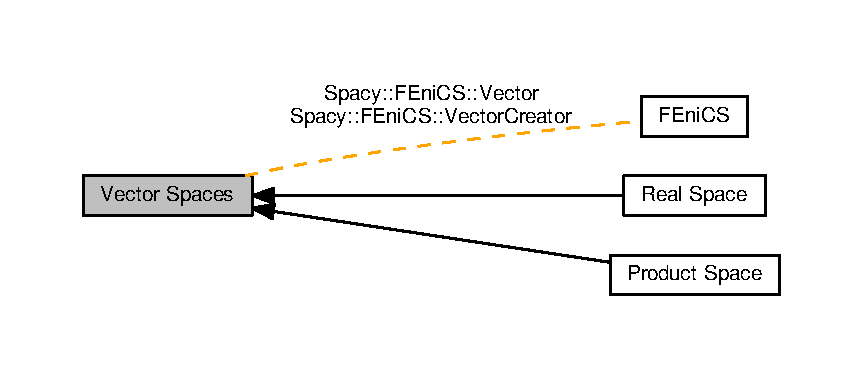
\includegraphics[width=350pt]{group__VectorSpaceGroup}
\end{center}
\end{figure}
\subsection*{Modules}
\begin{DoxyCompactItemize}
\item 
\hyperlink{group__RealGroup}{Real Space}
\begin{DoxyCompactList}\small\item\em A one dimensional vector space representing the space of real numbers. \end{DoxyCompactList}\item 
\hyperlink{group__ProductSpaceGroup}{Product Space}
\begin{DoxyCompactList}\small\item\em A product space that supports distinction between primal and dual variables. \end{DoxyCompactList}\end{DoxyCompactItemize}
\subsection*{Classes}
\begin{DoxyCompactItemize}
\item 
class \hyperlink{classSpacy_1_1FEniCS_1_1Vector}{Spacy\+::\+F\+Eni\+C\+S\+::\+Vector}
\begin{DoxyCompactList}\small\item\em Vector implementation for F\+Eni\+C\+S (single space). \end{DoxyCompactList}\item 
class \hyperlink{classSpacy_1_1FEniCS_1_1VectorCreator}{Spacy\+::\+F\+Eni\+C\+S\+::\+Vector\+Creator}
\begin{DoxyCompactList}\small\item\em Creator for vector space elements for F\+Eni\+C\+S. \end{DoxyCompactList}\end{DoxyCompactItemize}
\subsection*{Typedefs}
\begin{DoxyCompactItemize}
\item 
using \hyperlink{group__VectorSpaceGroup_gafda42fd5aa3f7597a42b9831bf4dfd07}{Spacy\+::\+Rn\+::\+Vector} = Generic\+::\+Vector$<$ \+::Eigen\+::\+Vector\+Xd $>$
\begin{DoxyCompactList}\small\item\em Vector for Rn, based on the Eigen library. \end{DoxyCompactList}\item 
using \hyperlink{group__VectorSpaceGroup_gab3b27cb653ec69d12c809394126b046a}{Spacy\+::\+Rn\+::\+Vector\+Creator} = Generic\+::\+Vector\+Creator$<$ \+::Eigen\+::\+Vector\+Xd $>$
\begin{DoxyCompactList}\small\item\em Vector creator for Rn, based on the Eigen library. \end{DoxyCompactList}\end{DoxyCompactItemize}
\subsection*{Functions}
\begin{DoxyCompactItemize}
\item 
{\footnotesize template$<$class... Args, class  = std\+::enable\+\_\+if\+\_\+t$<$std\+::is\+\_\+constructible$<$\+Description,\+Args...$>$\+::value$>$$>$ }\\\hyperlink{group__VectorSpaceGroup_ga89de372343310640870077e6167df3f4}{Spacy\+::\+Kaskade\+::\+Vector\+Creator$<$ Description $>$\+::\+Vector\+Creator} (Args \&\&...args)
\begin{DoxyCompactList}\small\item\em Create from Kaskade 7 function space. \end{DoxyCompactList}\item 
{\footnotesize template$<$class Description $>$ }\\auto \hyperlink{group__VectorSpaceGroup_ga04d45446864bbf87770d02eade7b64cf}{Spacy\+::\+Kaskade\+::make\+Hilbert\+Space} (const Description \&description)
\begin{DoxyCompactList}\small\item\em Create single space with hilbert space structure for Kaskade 7. \end{DoxyCompactList}\item 
{\footnotesize template$<$class Description $>$ }\\auto \hyperlink{group__VectorSpaceGroup_ga221db25c41371a2a823a6b569d735ef6}{Spacy\+::\+Kaskade\+::make\+Hilbert\+Space} (const Description \&description, const std\+::vector$<$ unsigned $>$ \&primal\+Ids, const std\+::vector$<$ unsigned $>$ \&dual\+Ids=\{\})
\begin{DoxyCompactList}\small\item\em Create product space with hilbert space structure for Kaskade 7. \end{DoxyCompactList}\end{DoxyCompactItemize}


\subsection{Detailed Description}
Collection of available vector spaces. 

Contains models for one-\/dimensional and product spaces as well as vector spaces for F\+Enics and Kaskade 7. 

\subsection{Typedef Documentation}
\hypertarget{group__VectorSpaceGroup_gafda42fd5aa3f7597a42b9831bf4dfd07}{}\index{Vector Spaces@{Vector Spaces}!Vector@{Vector}}
\index{Vector@{Vector}!Vector Spaces@{Vector Spaces}}
\subsubsection[{Vector}]{\setlength{\rightskip}{0pt plus 5cm}using {\bf Spacy\+::\+Rn\+::\+Vector} = typedef Generic\+::\+Vector$<$ \+::Eigen\+::\+Vector\+Xd $>$}\label{group__VectorSpaceGroup_gafda42fd5aa3f7597a42b9831bf4dfd07}


Vector for Rn, based on the Eigen library. 

, \hypertarget{group__VectorSpaceGroup_gab3b27cb653ec69d12c809394126b046a}{}\index{Vector Spaces@{Vector Spaces}!Vector\+Creator@{Vector\+Creator}}
\index{Vector\+Creator@{Vector\+Creator}!Vector Spaces@{Vector Spaces}}
\subsubsection[{Vector\+Creator}]{\setlength{\rightskip}{0pt plus 5cm}using {\bf Spacy\+::\+Rn\+::\+Vector\+Creator} = typedef Generic\+::\+Vector\+Creator$<$ \+::Eigen\+::\+Vector\+Xd $>$}\label{group__VectorSpaceGroup_gab3b27cb653ec69d12c809394126b046a}


Vector creator for Rn, based on the Eigen library. 

, 

\subsection{Function Documentation}
\hypertarget{group__VectorSpaceGroup_ga89de372343310640870077e6167df3f4}{}\index{Vector Spaces@{Vector Spaces}!Vector\+Creator@{Vector\+Creator}}
\index{Vector\+Creator@{Vector\+Creator}!Vector Spaces@{Vector Spaces}}
\subsubsection[{Vector\+Creator}]{\setlength{\rightskip}{0pt plus 5cm}template$<$class Description $>$ template$<$class... Args, class  = std\+::enable\+\_\+if\+\_\+t$<$std\+::is\+\_\+constructible$<$\+Description,\+Args...$>$\+::value$>$$>$ {\bf Spacy\+::\+Kaskade\+::\+Vector\+Creator}$<$ Description $>$\+::Vector\+Creator (
\begin{DoxyParamCaption}
\item[{Args \&\&...}]{args}
\end{DoxyParamCaption}
)\hspace{0.3cm}{\ttfamily [inline]}}\label{group__VectorSpaceGroup_ga89de372343310640870077e6167df3f4}


Create from Kaskade 7 function space. 


\begin{DoxyParams}{Parameters}
{\em space} & single Kaskade 7 function space (no product space) \\
\hline
\end{DoxyParams}
\hypertarget{group__VectorSpaceGroup_ga04d45446864bbf87770d02eade7b64cf}{}\index{Vector Spaces@{Vector Spaces}!make\+Hilbert\+Space@{make\+Hilbert\+Space}}
\index{make\+Hilbert\+Space@{make\+Hilbert\+Space}!Vector Spaces@{Vector Spaces}}
\subsubsection[{make\+Hilbert\+Space}]{\setlength{\rightskip}{0pt plus 5cm}template$<$class Description $>$ auto Spacy\+::\+Kaskade\+::make\+Hilbert\+Space (
\begin{DoxyParamCaption}
\item[{const Description \&}]{description}
\end{DoxyParamCaption}
)}\label{group__VectorSpaceGroup_ga04d45446864bbf87770d02eade7b64cf}


Create single space with hilbert space structure for Kaskade 7. 


\begin{DoxyParams}{Parameters}
{\em space} & single Kaskade 7 function space (no product space) \\
\hline
\end{DoxyParams}
\hypertarget{group__VectorSpaceGroup_ga221db25c41371a2a823a6b569d735ef6}{}\index{Vector Spaces@{Vector Spaces}!make\+Hilbert\+Space@{make\+Hilbert\+Space}}
\index{make\+Hilbert\+Space@{make\+Hilbert\+Space}!Vector Spaces@{Vector Spaces}}
\subsubsection[{make\+Hilbert\+Space}]{\setlength{\rightskip}{0pt plus 5cm}template$<$class Description $>$ auto Spacy\+::\+Kaskade\+::make\+Hilbert\+Space (
\begin{DoxyParamCaption}
\item[{const Description \&}]{description, }
\item[{const std\+::vector$<$ unsigned $>$ \&}]{primal\+Ids, }
\item[{const std\+::vector$<$ unsigned $>$ \&}]{dual\+Ids = {\ttfamily \{\}}}
\end{DoxyParamCaption}
)}\label{group__VectorSpaceGroup_ga221db25c41371a2a823a6b569d735ef6}


Create product space with hilbert space structure for Kaskade 7. 


\begin{DoxyParams}{Parameters}
{\em spaces} & boost fusion forward sequence of const pointers to Kaskade 7 function spaces \\
\hline
{\em primal\+Ids} & ids of primal variables \\
\hline
{\em dual\+Ids} & ids of dual variables \\
\hline
\end{DoxyParams}

\hypertarget{group__RealGroup}{}\section{Real Space}
\label{group__RealGroup}\index{Real Space@{Real Space}}


A one dimensional vector space representing the space of real numbers.  


Collaboration diagram for Real Space\+:\nopagebreak
\begin{figure}[H]
\begin{center}
\leavevmode
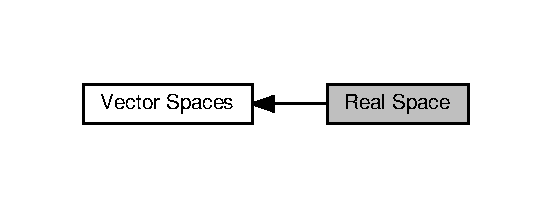
\includegraphics[width=265pt]{group__RealGroup}
\end{center}
\end{figure}
\subsection*{Classes}
\begin{DoxyCompactItemize}
\item 
class \hyperlink{classSpacy_1_1Real}{Spacy\+::\+Real}
\begin{DoxyCompactList}\small\item\em \hyperlink{classSpacy_1_1Real}{Real} number. \end{DoxyCompactList}\end{DoxyCompactItemize}
\subsection*{Functions}
\begin{DoxyCompactItemize}
\item 
Vector\+Space \hyperlink{group__RealGroup_gaa07f743f9874ecff062c511b7126f8b6_gaa07f743f9874ecff062c511b7126f8b6}{Spacy\+::\+Real\+Space\+::make\+Hilbert\+Space} (bool default\+Index=false)
\begin{DoxyCompactList}\small\item\em Construct space of real numbers. \end{DoxyCompactList}\end{DoxyCompactItemize}


\subsection{Detailed Description}
A one dimensional vector space representing the space of real numbers. 



\subsection{Function Documentation}
\hypertarget{group__RealGroup_gaa07f743f9874ecff062c511b7126f8b6_gaa07f743f9874ecff062c511b7126f8b6}{}\index{Real Space@{Real Space}!make\+Hilbert\+Space@{make\+Hilbert\+Space}}
\index{make\+Hilbert\+Space@{make\+Hilbert\+Space}!Real Space@{Real Space}}
\subsubsection[{make\+Hilbert\+Space}]{\setlength{\rightskip}{0pt plus 5cm}Vector\+Space Spacy\+::\+Real\+Space\+::make\+Hilbert\+Space (
\begin{DoxyParamCaption}
\item[{bool}]{default\+Index = {\ttfamily false}}
\end{DoxyParamCaption}
)}\label{group__RealGroup_gaa07f743f9874ecff062c511b7126f8b6_gaa07f743f9874ecff062c511b7126f8b6}


Construct space of real numbers. 

\begin{DoxyReturn}{Returns}
\hyperlink{group__SpacyGroup_ga63c49d211bf214be1fb321440ed03aad_ga63c49d211bf214be1fb321440ed03aad}{Spacy\+::make\+Hilbert\+Space()} \char`\"{}\+::\+Spacy\+::make\+Hilbert\+Space( \mbox{[}$\,$\mbox{]}(const Spacy$\ast$ space)\{ return Vector\{$\ast$space\}; \} , Scalar\+Product\{\} )\char`\"{} 
\end{DoxyReturn}

\hypertarget{group__ProductSpaceGroup}{}\section{Product Space}
\label{group__ProductSpaceGroup}\index{Product Space@{Product Space}}


A product space that supports distinction between primal and dual variables.  


Collaboration diagram for Product Space\+:\nopagebreak
\begin{figure}[H]
\begin{center}
\leavevmode
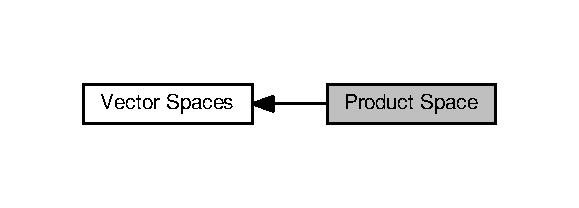
\includegraphics[width=278pt]{group__ProductSpaceGroup}
\end{center}
\end{figure}
\subsection*{Classes}
\begin{DoxyCompactItemize}
\item 
class \hyperlink{classSpacy_1_1ProductSpace_1_1ScalarProduct}{Spacy\+::\+Product\+Space\+::\+Scalar\+Product}
\begin{DoxyCompactList}\small\item\em Canonical scalar product on product spaces. \end{DoxyCompactList}\item 
class \hyperlink{classSpacy_1_1ProductSpace_1_1Vector}{Spacy\+::\+Product\+Space\+::\+Vector}
\begin{DoxyCompactList}\small\item\em Product space vector. \end{DoxyCompactList}\item 
class \hyperlink{classSpacy_1_1ProductSpace_1_1VectorCreator}{Spacy\+::\+Product\+Space\+::\+Vector\+Creator}
\begin{DoxyCompactList}\small\item\em Creator for \hyperlink{classSpacy_1_1ProductSpace_1_1Vector}{Product\+Space\+::\+Vector}. \end{DoxyCompactList}\end{DoxyCompactItemize}
\subsection*{Functions}
\begin{DoxyCompactItemize}
\item 
Vector\+Space \hyperlink{group__ProductSpaceGroup_gad4b421dd4563c7d575550ab4d5d3ff0d_gad4b421dd4563c7d575550ab4d5d3ff0d}{Spacy\+::\+Product\+Space\+::make\+Hilbert\+Space} (const std\+::vector$<$ std\+::shared\+\_\+ptr$<$ Vector\+Space $>$ $>$ \&spaces)
\begin{DoxyCompactList}\small\item\em Create product space from spaces. \end{DoxyCompactList}\item 
Vector\+Space \hyperlink{group__ProductSpaceGroup_ga24762c7baa8ea3a76af7c984874f7e37_ga24762c7baa8ea3a76af7c984874f7e37}{Spacy\+::\+Product\+Space\+::make\+Hilbert\+Space} (const std\+::vector$<$ std\+::shared\+\_\+ptr$<$ Vector\+Space $>$ $>$ \&spaces, const std\+::vector$<$ unsigned $>$ \&primal\+Sub\+Space\+Ids, const std\+::vector$<$ unsigned $>$ \&dual\+Sub\+Space\+Ids=\{\})
\begin{DoxyCompactList}\small\item\em Create product space from spaces. \end{DoxyCompactList}\end{DoxyCompactItemize}


\subsection{Detailed Description}
A product space that supports distinction between primal and dual variables. 



\subsection{Function Documentation}
\hypertarget{group__ProductSpaceGroup_gad4b421dd4563c7d575550ab4d5d3ff0d_gad4b421dd4563c7d575550ab4d5d3ff0d}{}\index{Product Space@{Product Space}!make\+Hilbert\+Space@{make\+Hilbert\+Space}}
\index{make\+Hilbert\+Space@{make\+Hilbert\+Space}!Product Space@{Product Space}}
\subsubsection[{make\+Hilbert\+Space}]{\setlength{\rightskip}{0pt plus 5cm}Vector\+Space Spacy\+::\+Product\+Space\+::make\+Hilbert\+Space (
\begin{DoxyParamCaption}
\item[{const std\+::vector$<$ std\+::shared\+\_\+ptr$<$ {\bf Vector\+Space} $>$ $>$ \&}]{spaces}
\end{DoxyParamCaption}
)}\label{group__ProductSpaceGroup_gad4b421dd4563c7d575550ab4d5d3ff0d_gad4b421dd4563c7d575550ab4d5d3ff0d}


Create product space from spaces. 


\begin{DoxyParams}{Parameters}
{\em spaces} & vector of spaces\\
\hline
\end{DoxyParams}
Creates a simple product space with only primal variables. \hypertarget{group__ProductSpaceGroup_ga24762c7baa8ea3a76af7c984874f7e37_ga24762c7baa8ea3a76af7c984874f7e37}{}\index{Product Space@{Product Space}!make\+Hilbert\+Space@{make\+Hilbert\+Space}}
\index{make\+Hilbert\+Space@{make\+Hilbert\+Space}!Product Space@{Product Space}}
\subsubsection[{make\+Hilbert\+Space}]{\setlength{\rightskip}{0pt plus 5cm}Vector\+Space Spacy\+::\+Product\+Space\+::make\+Hilbert\+Space (
\begin{DoxyParamCaption}
\item[{const std\+::vector$<$ std\+::shared\+\_\+ptr$<$ {\bf Vector\+Space} $>$ $>$ \&}]{spaces, }
\item[{const std\+::vector$<$ unsigned $>$ \&}]{primal\+Sub\+Space\+Ids, }
\item[{const std\+::vector$<$ unsigned $>$ \&}]{dual\+Sub\+Space\+Ids = {\ttfamily \{\}}}
\end{DoxyParamCaption}
)}\label{group__ProductSpaceGroup_ga24762c7baa8ea3a76af7c984874f7e37_ga24762c7baa8ea3a76af7c984874f7e37}


Create product space from spaces. 


\begin{DoxyParams}{Parameters}
{\em spaces} & vector of spaces \\
\hline
{\em primal\+Sub\+Space\+Ids} & entries of spaces that correspond to primal variables \\
\hline
{\em dual\+Sub\+Space\+Ids} & entries of spaces that correspond to dual variables \\
\hline
\end{DoxyParams}

\hypertarget{group__FenicsGroup}{}\section{Vector Space for F\+Eni\+C\+S}
\label{group__FenicsGroup}\index{Vector Space for F\+Eni\+C\+S@{Vector Space for F\+Eni\+C\+S}}


Vector spaces, functionals and operators for \href{http://www.fenicsproject.org}{\tt F\+Eni\+C\+S}.  


Collaboration diagram for Vector Space for F\+Eni\+C\+S\+:\nopagebreak
\begin{figure}[H]
\begin{center}
\leavevmode
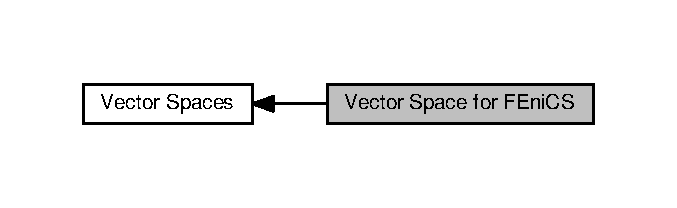
\includegraphics[width=325pt]{group__FenicsGroup}
\end{center}
\end{figure}
\subsection*{Classes}
\begin{DoxyCompactItemize}
\item 
class \hyperlink{classSpacy_1_1FEniCS_1_1C1Operator}{Spacy\+::\+F\+Eni\+C\+S\+::\+C1\+Operator$<$ Residual\+Form, Jacobian\+Form $>$}
\begin{DoxyCompactList}\small\item\em Operator interface for F\+Eni\+C\+S. Models a differentiable operator $A:X\rightarrow Y$. \end{DoxyCompactList}\item 
class \hyperlink{classSpacy_1_1FEniCS_1_1C2Functional}{Spacy\+::\+F\+Eni\+C\+S\+::\+C2\+Functional$<$ F, D\+F, D\+D\+F $>$}
\begin{DoxyCompactList}\small\item\em Functional interface for F\+Eni\+C\+S. Models a twice differentiable functional $f:X\rightarrow \mathbb{R}$. \end{DoxyCompactList}\item 
class \hyperlink{classSpacy_1_1FEniCS_1_1DynamicC1Operator}{Spacy\+::\+F\+Eni\+C\+S\+::\+Dynamic\+C1\+Operator$<$ Residual\+Form, Jacobian\+Form, Mass\+Form, Source $>$}
\begin{DoxyCompactList}\small\item\em Operator interface for F\+Eni\+C\+S. Models a differentiable operator $A:X\rightarrow Y$. \end{DoxyCompactList}\item 
class \hyperlink{classSpacy_1_1FEniCS_1_1l2Product}{Spacy\+::\+F\+Eni\+C\+S\+::l2\+Product}
\begin{DoxyCompactList}\small\item\em l2 product $(x,y) = \sum_i x_i y_i $ for F\+Eni\+C\+S. \end{DoxyCompactList}\item 
class \hyperlink{classSpacy_1_1FEniCS_1_1LinearOperator}{Spacy\+::\+F\+Eni\+C\+S\+::\+Linear\+Operator}
\begin{DoxyCompactList}\small\item\em Linear operator interface for operators in F\+Eni\+C\+S. \end{DoxyCompactList}\item 
class \hyperlink{classSpacy_1_1FEniCS_1_1LUSolver}{Spacy\+::\+F\+Eni\+C\+S\+::\+L\+U\+Solver}
\begin{DoxyCompactList}\small\item\em L\+U solver for F\+Eni\+C\+S. \end{DoxyCompactList}\item 
class \hyperlink{classSpacy_1_1FEniCS_1_1TransposedLUSolver}{Spacy\+::\+F\+Eni\+C\+S\+::\+Transposed\+L\+U\+Solver}
\begin{DoxyCompactList}\small\item\em Transposed L\+U solver for F\+Eni\+C\+S. \end{DoxyCompactList}\item 
class \hyperlink{classSpacy_1_1FEniCS_1_1Vector}{Spacy\+::\+F\+Eni\+C\+S\+::\+Vector}
\begin{DoxyCompactList}\small\item\em Vector implementation for F\+Eni\+C\+S (single space). \end{DoxyCompactList}\item 
class \hyperlink{classSpacy_1_1FEniCS_1_1VectorCreator}{Spacy\+::\+F\+Eni\+C\+S\+::\+Vector\+Creator}
\begin{DoxyCompactList}\small\item\em Creator for vector space elements for F\+Eni\+C\+S. See \hyperlink{group__SpacyGroup_ga1f5316487c031a478247206764bb2efb_VectorCreatorAnchor}{\+:\+:Spacy\+:\+:Vector\+Creator}, \hyperlink{group__ConceptGroup_ga3064301642b7c66b1b08f88a12a04645_VectorCreatorConceptAnchor}{\+:\+:Spacy\+:\+:Vector\+Creator\+Concept}. \end{DoxyCompactList}\end{DoxyCompactItemize}
\subsection*{Functions}
\begin{DoxyCompactItemize}
\item 
{\footnotesize template$<$class Residual\+Form , class Jacobian\+Form $>$ }\\auto \hyperlink{group__FenicsGroup_ga5b21d39905318b5e3f36b71c1fb525e9_ga5b21d39905318b5e3f36b71c1fb525e9}{Spacy\+::\+F\+Eni\+C\+S\+::make\+C1\+Operator} (Residual\+Form \&F, Jacobian\+Form \&J, const std\+::vector$<$ const dolfin\+::\+Dirichlet\+B\+C $\ast$ $>$ \&bcs, Vector\+Space \&domain, Vector\+Space \&range)
\begin{DoxyCompactList}\small\item\em Convenient generation of a differentiable operator $A: X\rightarrow Y$ as used in F\+Eni\+C\+S. \end{DoxyCompactList}\item 
{\footnotesize template$<$class Residual\+Form , class Jacobian\+Form $>$ }\\auto \hyperlink{group__FenicsGroup_gaecd46636694770dba7c8f99325341eda_gaecd46636694770dba7c8f99325341eda}{Spacy\+::\+F\+Eni\+C\+S\+::make\+C1\+Operator} (Residual\+Form \&F, Jacobian\+Form \&J, Vector\+Space \&domain, Vector\+Space \&range)
\begin{DoxyCompactList}\small\item\em Convenient generation of a differentiable operator $A: X\rightarrow Y$ from F\+Eni\+C\+S(dolfin). \end{DoxyCompactList}\item 
{\footnotesize template$<$class Residual\+Form , class Jacobian\+Form $>$ }\\auto \hyperlink{group__FenicsGroup_gafc3de3603a9ac312096d742da2b5752b_gafc3de3603a9ac312096d742da2b5752b}{Spacy\+::\+F\+Eni\+C\+S\+::make\+C1\+Operator} (Residual\+Form \&F, Jacobian\+Form \&J, const std\+::vector$<$ const dolfin\+::\+Dirichlet\+B\+C $\ast$ $>$ \&bcs, Vector\+Space \&space)
\begin{DoxyCompactList}\small\item\em Convenient generation of a differentiable operator $A: X\rightarrow X$ from F\+Eni\+C\+S(dolfin). \end{DoxyCompactList}\item 
{\footnotesize template$<$class Residual\+Form , class Jacobian\+Form $>$ }\\auto \hyperlink{group__FenicsGroup_ga508af586ecdbc9f099759ffec06e99df_ga508af586ecdbc9f099759ffec06e99df}{Spacy\+::\+F\+Eni\+C\+S\+::make\+C1\+Operator} (Residual\+Form \&F, Jacobian\+Form \&J, Vector\+Space \&space)
\begin{DoxyCompactList}\small\item\em Convenient generation of a differentiable operator $A: X\rightarrow X$ from F\+Eni\+C\+S(dolfin). \end{DoxyCompactList}\item 
{\footnotesize template$<$class F , class D\+F , class D\+D\+F $>$ }\\auto \hyperlink{group__FenicsGroup_ga78db716003d17d5f781dfcb13a183519_ga78db716003d17d5f781dfcb13a183519}{Spacy\+::\+F\+Eni\+C\+S\+::make\+C2\+Functional} (const F \&f, const D\+F \&J, const D\+D\+F \&H, const std\+::vector$<$ const dolfin\+::\+Dirichlet\+B\+C $\ast$ $>$ \&bcs, const Vector\+Space \&space)
\begin{DoxyCompactList}\small\item\em Convenient generation of a twice differentiable functional $f: X\rightarrow \mathbb{R}$ as used in F\+Eni\+C\+S. \end{DoxyCompactList}\item 
{\footnotesize template$<$class F , class D\+F , class D\+D\+F $>$ }\\auto \hyperlink{group__FenicsGroup_ga4e69e5b7265feac21653bfc2da725a75_ga4e69e5b7265feac21653bfc2da725a75}{Spacy\+::\+F\+Eni\+C\+S\+::make\+C2\+Functional} (const F \&f, const D\+F \&J, const D\+D\+F \&H, const Vector\+Space \&space)
\begin{DoxyCompactList}\small\item\em Convenient generation of a twice differentiable functional $f: X\rightarrow \mathbb{R}$ with out Dirichlet boundary conditions as used in F\+Eni\+C\+S. \end{DoxyCompactList}\item 
{\footnotesize template$<$class Residual\+Form , class Jacobian\+Form , class Mass\+Form , class Source $>$ }\\auto \hyperlink{group__FenicsGroup_ga70d8ba7fecc2caba97343f5506340602_ga70d8ba7fecc2caba97343f5506340602}{Spacy\+::\+F\+Eni\+C\+S\+::make\+Dynamic\+C1\+Operator} (Residual\+Form \&\&F, Jacobian\+Form \&\&J, Mass\+Form \&\&M, Source \&\&f, const Vector\+Space \&domain, const Vector\+Space \&range)
\begin{DoxyCompactList}\small\item\em Convenient generation of a differentiable operator $A: X\rightarrow Y$ as used in F\+Eni\+C\+S. \end{DoxyCompactList}\item 
{\footnotesize template$<$class Residual\+Form , class Jacobian\+Form , class Mass\+Form , class Source $>$ }\\auto \hyperlink{group__FenicsGroup_ga467a0e85b66c8f17cdaf2884d5d443cd_ga467a0e85b66c8f17cdaf2884d5d443cd}{Spacy\+::\+F\+Eni\+C\+S\+::make\+Dynamic\+C1\+Operator} (Residual\+Form \&\&F, Jacobian\+Form \&\&J, Mass\+Form \&\&M, Source \&\&f, const Vector\+Space \&domain)
\begin{DoxyCompactList}\small\item\em Convenient generation of a differentiable operator $A: X\rightarrow Y$ from F\+Eni\+C\+S(dolfin). \end{DoxyCompactList}\item 
void \hyperlink{group__FenicsGroup_gab3d4c7c1e91a50e4e816598258b6edce_gab3d4c7c1e91a50e4e816598258b6edce}{Spacy\+::\+F\+Eni\+C\+S\+::copy\+Coefficients} (const dolfin\+::\+Form \&F, dolfin\+::\+Form \&G)
\begin{DoxyCompactList}\small\item\em Copy coefficients of F to G. \end{DoxyCompactList}\item 
void \hyperlink{group__FenicsGroup_ga7f43f0c660d0646adb031b453c536bb0_ga7f43f0c660d0646adb031b453c536bb0}{Spacy\+::\+F\+Eni\+C\+S\+::copy} (const \+::\hyperlink{classSpacy_1_1Vector}{Spacy\+::\+Vector} \&x, dolfin\+::\+Generic\+Vector \&y)
\begin{DoxyCompactList}\small\item\em Copy from \hyperlink{group__SpacyGroup_gafc144d2730ef87a67e54f8cd750b1f54_VectorAnchor}{\+:\+:Spacy\+:\+:Vector} to dolfin\+::\+Generic\+Vector. \end{DoxyCompactList}\item 
void \hyperlink{group__FenicsGroup_ga28fb1ebae29e07ec0256bb2331599aa7_ga28fb1ebae29e07ec0256bb2331599aa7}{Spacy\+::\+F\+Eni\+C\+S\+::copy} (const \+::\hyperlink{classSpacy_1_1Vector}{Spacy\+::\+Vector} \&x, dolfin\+::\+Function \&y)
\begin{DoxyCompactList}\small\item\em Copy from \hyperlink{group__SpacyGroup_gafc144d2730ef87a67e54f8cd750b1f54_VectorAnchor}{\+:\+:Spacy\+:\+:Vector} to dolfin\+::\+Function. \end{DoxyCompactList}\item 
void \hyperlink{group__FenicsGroup_ga61c5e45dbb789c155fbf86f8ec288f17_ga61c5e45dbb789c155fbf86f8ec288f17}{Spacy\+::\+F\+Eni\+C\+S\+::copy} (const dolfin\+::\+Generic\+Vector \&y,\+::\hyperlink{classSpacy_1_1Vector}{Spacy\+::\+Vector} \&x)
\begin{DoxyCompactList}\small\item\em Copy from dolfin\+::\+Generic\+Vector to \hyperlink{group__SpacyGroup_gafc144d2730ef87a67e54f8cd750b1f54_VectorAnchor}{\+:\+:Spacy\+:\+:Vector}. \end{DoxyCompactList}\item 
Vector\+Space \hyperlink{group__FenicsGroup_ga89defe8c7e08ab224af2a3cd0445e254_ga89defe8c7e08ab224af2a3cd0445e254}{Spacy\+::\+F\+Eni\+C\+S\+::make\+Hilbert\+Space} (const dolfin\+::\+Function\+Space \&space)
\begin{DoxyCompactList}\small\item\em Convenient generation of a single vector space from dolfin\+::\+Function\+Space. \end{DoxyCompactList}\item 
Vector\+Space \hyperlink{group__FenicsGroup_ga1aaf48bfbd005bee810090a01404ab4a_ga1aaf48bfbd005bee810090a01404ab4a}{Spacy\+::\+F\+Eni\+C\+S\+::make\+Hilbert\+Space} (const dolfin\+::\+Function\+Space \&space, const std\+::unordered\+\_\+map$<$ std\+::size\+\_\+t, std\+::size\+\_\+t $>$ \&dofmap)
\begin{DoxyCompactList}\small\item\em Convenient generation of a single vector space from dolfin\+::\+Function\+Space. \end{DoxyCompactList}\item 
Vector\+Space \hyperlink{group__FenicsGroup_gaa16b365c49ec0660e5f707ad7da38a75_gaa16b365c49ec0660e5f707ad7da38a75}{Spacy\+::\+F\+Eni\+C\+S\+::make\+Hilbert\+Space} (const dolfin\+::\+Function\+Space \&space, const std\+::vector$<$ unsigned $>$ \&primal\+Ids, const std\+::vector$<$ unsigned $>$ \&dual\+Ids=\{\})
\begin{DoxyCompactList}\small\item\em Convenient generation of a product space from dolfin\+::\+Function\+Space. \end{DoxyCompactList}\end{DoxyCompactItemize}


\subsection{Detailed Description}
Vector spaces, functionals and operators for \href{http://www.fenicsproject.org}{\tt F\+Eni\+C\+S}. 



\subsection{Function Documentation}
\hypertarget{group__FenicsGroup_ga7f43f0c660d0646adb031b453c536bb0_ga7f43f0c660d0646adb031b453c536bb0}{}\index{Vector Space for F\+Eni\+C\+S@{Vector Space for F\+Eni\+C\+S}!copy@{copy}}
\index{copy@{copy}!Vector Space for F\+Eni\+C\+S@{Vector Space for F\+Eni\+C\+S}}
\subsubsection[{copy}]{\setlength{\rightskip}{0pt plus 5cm}void Spacy\+::\+F\+Eni\+C\+S\+::copy (
\begin{DoxyParamCaption}
\item[{const \+::{\bf Spacy\+::\+Vector} \&}]{x, }
\item[{dolfin\+::\+Generic\+Vector \&}]{y}
\end{DoxyParamCaption}
)}\label{group__FenicsGroup_ga7f43f0c660d0646adb031b453c536bb0_ga7f43f0c660d0646adb031b453c536bb0}


Copy from \hyperlink{group__SpacyGroup_gafc144d2730ef87a67e54f8cd750b1f54_VectorAnchor}{\+:\+:Spacy\+:\+:Vector} to dolfin\+::\+Generic\+Vector. 

Does consider product space structures. \begin{DoxySeeAlso}{See also}
Product\+Space 
\end{DoxySeeAlso}
\hypertarget{group__FenicsGroup_ga28fb1ebae29e07ec0256bb2331599aa7_ga28fb1ebae29e07ec0256bb2331599aa7}{}\index{Vector Space for F\+Eni\+C\+S@{Vector Space for F\+Eni\+C\+S}!copy@{copy}}
\index{copy@{copy}!Vector Space for F\+Eni\+C\+S@{Vector Space for F\+Eni\+C\+S}}
\subsubsection[{copy}]{\setlength{\rightskip}{0pt plus 5cm}void Spacy\+::\+F\+Eni\+C\+S\+::copy (
\begin{DoxyParamCaption}
\item[{const \+::{\bf Spacy\+::\+Vector} \&}]{x, }
\item[{dolfin\+::\+Function \&}]{y}
\end{DoxyParamCaption}
)}\label{group__FenicsGroup_ga28fb1ebae29e07ec0256bb2331599aa7_ga28fb1ebae29e07ec0256bb2331599aa7}


Copy from \hyperlink{group__SpacyGroup_gafc144d2730ef87a67e54f8cd750b1f54_VectorAnchor}{\+:\+:Spacy\+:\+:Vector} to dolfin\+::\+Function. 

Does consider product space structures. \begin{DoxySeeAlso}{See also}
Product\+Space 
\end{DoxySeeAlso}
\hypertarget{group__FenicsGroup_ga61c5e45dbb789c155fbf86f8ec288f17_ga61c5e45dbb789c155fbf86f8ec288f17}{}\index{Vector Space for F\+Eni\+C\+S@{Vector Space for F\+Eni\+C\+S}!copy@{copy}}
\index{copy@{copy}!Vector Space for F\+Eni\+C\+S@{Vector Space for F\+Eni\+C\+S}}
\subsubsection[{copy}]{\setlength{\rightskip}{0pt plus 5cm}void Spacy\+::\+F\+Eni\+C\+S\+::copy (
\begin{DoxyParamCaption}
\item[{const dolfin\+::\+Generic\+Vector \&}]{y, }
\item[{\+::{\bf Spacy\+::\+Vector} \&}]{x}
\end{DoxyParamCaption}
)}\label{group__FenicsGroup_ga61c5e45dbb789c155fbf86f8ec288f17_ga61c5e45dbb789c155fbf86f8ec288f17}


Copy from dolfin\+::\+Generic\+Vector to \hyperlink{group__SpacyGroup_gafc144d2730ef87a67e54f8cd750b1f54_VectorAnchor}{\+:\+:Spacy\+:\+:Vector}. 

Does consider product space structures. \begin{DoxySeeAlso}{See also}
\hyperlink{group__ProductSpaceGroup}{Product Space} 
\end{DoxySeeAlso}
\hypertarget{group__FenicsGroup_gab3d4c7c1e91a50e4e816598258b6edce_gab3d4c7c1e91a50e4e816598258b6edce}{}\index{Vector Space for F\+Eni\+C\+S@{Vector Space for F\+Eni\+C\+S}!copy\+Coefficients@{copy\+Coefficients}}
\index{copy\+Coefficients@{copy\+Coefficients}!Vector Space for F\+Eni\+C\+S@{Vector Space for F\+Eni\+C\+S}}
\subsubsection[{copy\+Coefficients}]{\setlength{\rightskip}{0pt plus 5cm}void Spacy\+::\+F\+Eni\+C\+S\+::copy\+Coefficients (
\begin{DoxyParamCaption}
\item[{const dolfin\+::\+Form \&}]{F, }
\item[{dolfin\+::\+Form \&}]{G}
\end{DoxyParamCaption}
)}\label{group__FenicsGroup_gab3d4c7c1e91a50e4e816598258b6edce_gab3d4c7c1e91a50e4e816598258b6edce}


Copy coefficients of F to G. 

Whatever the copy-\/constructor for dolfin forms does it does not copy. So if you want to copy these do the following. Create A new form from the function spaces stored in G. Then copy the coefficients with this function. \hypertarget{group__FenicsGroup_ga5b21d39905318b5e3f36b71c1fb525e9_ga5b21d39905318b5e3f36b71c1fb525e9}{}\index{Vector Space for F\+Eni\+C\+S@{Vector Space for F\+Eni\+C\+S}!make\+C1\+Operator@{make\+C1\+Operator}}
\index{make\+C1\+Operator@{make\+C1\+Operator}!Vector Space for F\+Eni\+C\+S@{Vector Space for F\+Eni\+C\+S}}
\subsubsection[{make\+C1\+Operator}]{\setlength{\rightskip}{0pt plus 5cm}template$<$class Residual\+Form , class Jacobian\+Form $>$ auto Spacy\+::\+F\+Eni\+C\+S\+::make\+C1\+Operator (
\begin{DoxyParamCaption}
\item[{Residual\+Form \&}]{F, }
\item[{Jacobian\+Form \&}]{J, }
\item[{const std\+::vector$<$ const dolfin\+::\+Dirichlet\+B\+C $\ast$ $>$ \&}]{bcs, }
\item[{{\bf Vector\+Space} \&}]{domain, }
\item[{{\bf Vector\+Space} \&}]{range}
\end{DoxyParamCaption}
)}\label{group__FenicsGroup_ga5b21d39905318b5e3f36b71c1fb525e9_ga5b21d39905318b5e3f36b71c1fb525e9}


Convenient generation of a differentiable operator $A: X\rightarrow Y$ as used in F\+Eni\+C\+S. 

\begin{DoxyReturn}{Returns}
\hyperlink{classSpacy_1_1FEniCS_1_1C1Operator}{\+:\+:Spacy\+:\+:Fenics\+:\+:C1\+Operator$<$Residual\+Form,Jacobian\+Form$>$( F , J , bcs , domain , range )} 
\end{DoxyReturn}
\hypertarget{group__FenicsGroup_gaecd46636694770dba7c8f99325341eda_gaecd46636694770dba7c8f99325341eda}{}\index{Vector Space for F\+Eni\+C\+S@{Vector Space for F\+Eni\+C\+S}!make\+C1\+Operator@{make\+C1\+Operator}}
\index{make\+C1\+Operator@{make\+C1\+Operator}!Vector Space for F\+Eni\+C\+S@{Vector Space for F\+Eni\+C\+S}}
\subsubsection[{make\+C1\+Operator}]{\setlength{\rightskip}{0pt plus 5cm}template$<$class Residual\+Form , class Jacobian\+Form $>$ auto Spacy\+::\+F\+Eni\+C\+S\+::make\+C1\+Operator (
\begin{DoxyParamCaption}
\item[{Residual\+Form \&}]{F, }
\item[{Jacobian\+Form \&}]{J, }
\item[{{\bf Vector\+Space} \&}]{domain, }
\item[{{\bf Vector\+Space} \&}]{range}
\end{DoxyParamCaption}
)}\label{group__FenicsGroup_gaecd46636694770dba7c8f99325341eda_gaecd46636694770dba7c8f99325341eda}


Convenient generation of a differentiable operator $A: X\rightarrow Y$ from F\+Eni\+C\+S(dolfin). 

\begin{DoxyReturn}{Returns}
\hyperlink{classSpacy_1_1FEniCS_1_1C1Operator}{\+:\+:Spacy\+:\+:Fenics\+:\+:C1\+Operator$<$Residual\+Form,Jacobian\+Form$>$( F , J , domain , range )} 
\end{DoxyReturn}
\hypertarget{group__FenicsGroup_gafc3de3603a9ac312096d742da2b5752b_gafc3de3603a9ac312096d742da2b5752b}{}\index{Vector Space for F\+Eni\+C\+S@{Vector Space for F\+Eni\+C\+S}!make\+C1\+Operator@{make\+C1\+Operator}}
\index{make\+C1\+Operator@{make\+C1\+Operator}!Vector Space for F\+Eni\+C\+S@{Vector Space for F\+Eni\+C\+S}}
\subsubsection[{make\+C1\+Operator}]{\setlength{\rightskip}{0pt plus 5cm}template$<$class Residual\+Form , class Jacobian\+Form $>$ auto Spacy\+::\+F\+Eni\+C\+S\+::make\+C1\+Operator (
\begin{DoxyParamCaption}
\item[{Residual\+Form \&}]{F, }
\item[{Jacobian\+Form \&}]{J, }
\item[{const std\+::vector$<$ const dolfin\+::\+Dirichlet\+B\+C $\ast$ $>$ \&}]{bcs, }
\item[{{\bf Vector\+Space} \&}]{space}
\end{DoxyParamCaption}
)}\label{group__FenicsGroup_gafc3de3603a9ac312096d742da2b5752b_gafc3de3603a9ac312096d742da2b5752b}


Convenient generation of a differentiable operator $A: X\rightarrow X$ from F\+Eni\+C\+S(dolfin). 

\begin{DoxyReturn}{Returns}
\hyperlink{classSpacy_1_1FEniCS_1_1C1Operator}{\+:\+:Spacy\+:\+:Fenics\+:\+:C1\+Operator$<$Residual\+Form,Jacobian\+Form$>$( F , J , bcs , space , space )} 
\end{DoxyReturn}
\hypertarget{group__FenicsGroup_ga508af586ecdbc9f099759ffec06e99df_ga508af586ecdbc9f099759ffec06e99df}{}\index{Vector Space for F\+Eni\+C\+S@{Vector Space for F\+Eni\+C\+S}!make\+C1\+Operator@{make\+C1\+Operator}}
\index{make\+C1\+Operator@{make\+C1\+Operator}!Vector Space for F\+Eni\+C\+S@{Vector Space for F\+Eni\+C\+S}}
\subsubsection[{make\+C1\+Operator}]{\setlength{\rightskip}{0pt plus 5cm}template$<$class Residual\+Form , class Jacobian\+Form $>$ auto Spacy\+::\+F\+Eni\+C\+S\+::make\+C1\+Operator (
\begin{DoxyParamCaption}
\item[{Residual\+Form \&}]{F, }
\item[{Jacobian\+Form \&}]{J, }
\item[{{\bf Vector\+Space} \&}]{space}
\end{DoxyParamCaption}
)}\label{group__FenicsGroup_ga508af586ecdbc9f099759ffec06e99df_ga508af586ecdbc9f099759ffec06e99df}


Convenient generation of a differentiable operator $A: X\rightarrow X$ from F\+Eni\+C\+S(dolfin). 

\begin{DoxyReturn}{Returns}
\hyperlink{classSpacy_1_1FEniCS_1_1C1Operator}{Fenics\+:\+:C1\+Operator$<$Residual\+Form,Jacobian\+Form$>$( F , J , space , space )} 
\end{DoxyReturn}
\hypertarget{group__FenicsGroup_ga78db716003d17d5f781dfcb13a183519_ga78db716003d17d5f781dfcb13a183519}{}\index{Vector Space for F\+Eni\+C\+S@{Vector Space for F\+Eni\+C\+S}!make\+C2\+Functional@{make\+C2\+Functional}}
\index{make\+C2\+Functional@{make\+C2\+Functional}!Vector Space for F\+Eni\+C\+S@{Vector Space for F\+Eni\+C\+S}}
\subsubsection[{make\+C2\+Functional}]{\setlength{\rightskip}{0pt plus 5cm}template$<$class F , class D\+F , class D\+D\+F $>$ auto Spacy\+::\+F\+Eni\+C\+S\+::make\+C2\+Functional (
\begin{DoxyParamCaption}
\item[{const F \&}]{f, }
\item[{const D\+F \&}]{J, }
\item[{const D\+D\+F \&}]{H, }
\item[{const std\+::vector$<$ const dolfin\+::\+Dirichlet\+B\+C $\ast$ $>$ \&}]{bcs, }
\item[{const {\bf Vector\+Space} \&}]{space}
\end{DoxyParamCaption}
)}\label{group__FenicsGroup_ga78db716003d17d5f781dfcb13a183519_ga78db716003d17d5f781dfcb13a183519}


Convenient generation of a twice differentiable functional $f: X\rightarrow \mathbb{R}$ as used in F\+Eni\+C\+S. 


\begin{DoxyParams}{Parameters}
{\em f} & form for the evaluation of $f$. \\
\hline
{\em J} & form for the evaluation of $f'$ \\
\hline
{\em H} & form for the evaluation of $f''$ \\
\hline
{\em bcs} & Dirichlet boundary conditions \\
\hline
{\em space} & domain space $X$ \\
\hline
\end{DoxyParams}
\begin{DoxyReturn}{Returns}
\hyperlink{classSpacy_1_1FEniCS_1_1C2Functional}{\+:\+:Spacy\+:\+:Fenics\+:\+:C2\+Functional$<$F,D\+F,D\+D\+F$>$( f , J , H , bcs , space )} 
\end{DoxyReturn}
\hypertarget{group__FenicsGroup_ga4e69e5b7265feac21653bfc2da725a75_ga4e69e5b7265feac21653bfc2da725a75}{}\index{Vector Space for F\+Eni\+C\+S@{Vector Space for F\+Eni\+C\+S}!make\+C2\+Functional@{make\+C2\+Functional}}
\index{make\+C2\+Functional@{make\+C2\+Functional}!Vector Space for F\+Eni\+C\+S@{Vector Space for F\+Eni\+C\+S}}
\subsubsection[{make\+C2\+Functional}]{\setlength{\rightskip}{0pt plus 5cm}template$<$class F , class D\+F , class D\+D\+F $>$ auto Spacy\+::\+F\+Eni\+C\+S\+::make\+C2\+Functional (
\begin{DoxyParamCaption}
\item[{const F \&}]{f, }
\item[{const D\+F \&}]{J, }
\item[{const D\+D\+F \&}]{H, }
\item[{const {\bf Vector\+Space} \&}]{space}
\end{DoxyParamCaption}
)}\label{group__FenicsGroup_ga4e69e5b7265feac21653bfc2da725a75_ga4e69e5b7265feac21653bfc2da725a75}


Convenient generation of a twice differentiable functional $f: X\rightarrow \mathbb{R}$ with out Dirichlet boundary conditions as used in F\+Eni\+C\+S. 


\begin{DoxyParams}{Parameters}
{\em f} & form for the evaluation of $f$. \\
\hline
{\em J} & form for the evaluation of $f'$ \\
\hline
{\em H} & form for the evaluation of $f''$ \\
\hline
{\em space} & domain space $X$ \\
\hline
\end{DoxyParams}
\begin{DoxyReturn}{Returns}
\hyperlink{classSpacy_1_1FEniCS_1_1C2Functional}{\+:\+:Spacy\+:\+:Fenics\+:\+:C2\+Functional$<$F,D\+F,D\+D\+F$>$( f , J , H , bcs , space )} 
\end{DoxyReturn}
\hypertarget{group__FenicsGroup_ga70d8ba7fecc2caba97343f5506340602_ga70d8ba7fecc2caba97343f5506340602}{}\index{Vector Space for F\+Eni\+C\+S@{Vector Space for F\+Eni\+C\+S}!make\+Dynamic\+C1\+Operator@{make\+Dynamic\+C1\+Operator}}
\index{make\+Dynamic\+C1\+Operator@{make\+Dynamic\+C1\+Operator}!Vector Space for F\+Eni\+C\+S@{Vector Space for F\+Eni\+C\+S}}
\subsubsection[{make\+Dynamic\+C1\+Operator}]{\setlength{\rightskip}{0pt plus 5cm}template$<$class Residual\+Form , class Jacobian\+Form , class Mass\+Form , class Source $>$ auto Spacy\+::\+F\+Eni\+C\+S\+::make\+Dynamic\+C1\+Operator (
\begin{DoxyParamCaption}
\item[{Residual\+Form \&\&}]{F, }
\item[{Jacobian\+Form \&\&}]{J, }
\item[{Mass\+Form \&\&}]{M, }
\item[{Source \&\&}]{f, }
\item[{const {\bf Vector\+Space} \&}]{domain, }
\item[{const {\bf Vector\+Space} \&}]{range}
\end{DoxyParamCaption}
)}\label{group__FenicsGroup_ga70d8ba7fecc2caba97343f5506340602_ga70d8ba7fecc2caba97343f5506340602}


Convenient generation of a differentiable operator $A: X\rightarrow Y$ as used in F\+Eni\+C\+S. 

\begin{DoxyReturn}{Returns}
\hyperlink{classSpacy_1_1FEniCS_1_1C1Operator}{\+:\+:Spacy\+:\+:Fenics\+:\+:C1\+Operator$<$Residual\+Form,Jacobian\+Form$>$( F , J , bcs , domain , range )}
\end{DoxyReturn}
Convenient generation of a differentiable operator $A: X\rightarrow Y$ from F\+Eni\+C\+S(dolfin). \begin{DoxyReturn}{Returns}
\hyperlink{classSpacy_1_1FEniCS_1_1C1Operator}{\+:\+:Spacy\+:\+:Fenics\+:\+:C1\+Operator$<$Residual\+Form,Jacobian\+Form$>$( F , J , domain , range )} 
\end{DoxyReturn}
\hypertarget{group__FenicsGroup_ga467a0e85b66c8f17cdaf2884d5d443cd_ga467a0e85b66c8f17cdaf2884d5d443cd}{}\index{Vector Space for F\+Eni\+C\+S@{Vector Space for F\+Eni\+C\+S}!make\+Dynamic\+C1\+Operator@{make\+Dynamic\+C1\+Operator}}
\index{make\+Dynamic\+C1\+Operator@{make\+Dynamic\+C1\+Operator}!Vector Space for F\+Eni\+C\+S@{Vector Space for F\+Eni\+C\+S}}
\subsubsection[{make\+Dynamic\+C1\+Operator}]{\setlength{\rightskip}{0pt plus 5cm}template$<$class Residual\+Form , class Jacobian\+Form , class Mass\+Form , class Source $>$ auto Spacy\+::\+F\+Eni\+C\+S\+::make\+Dynamic\+C1\+Operator (
\begin{DoxyParamCaption}
\item[{Residual\+Form \&\&}]{F, }
\item[{Jacobian\+Form \&\&}]{J, }
\item[{Mass\+Form \&\&}]{M, }
\item[{Source \&\&}]{f, }
\item[{const {\bf Vector\+Space} \&}]{domain}
\end{DoxyParamCaption}
)}\label{group__FenicsGroup_ga467a0e85b66c8f17cdaf2884d5d443cd_ga467a0e85b66c8f17cdaf2884d5d443cd}


Convenient generation of a differentiable operator $A: X\rightarrow Y$ from F\+Eni\+C\+S(dolfin). 

\begin{DoxyReturn}{Returns}
\hyperlink{classSpacy_1_1FEniCS_1_1C1Operator}{\+:\+:Spacy\+:\+:Fenics\+:\+:C1\+Operator$<$Residual\+Form,Jacobian\+Form$>$( F , J , domain , range )} 
\end{DoxyReturn}
\hypertarget{group__FenicsGroup_ga89defe8c7e08ab224af2a3cd0445e254_ga89defe8c7e08ab224af2a3cd0445e254}{}\index{Vector Space for F\+Eni\+C\+S@{Vector Space for F\+Eni\+C\+S}!make\+Hilbert\+Space@{make\+Hilbert\+Space}}
\index{make\+Hilbert\+Space@{make\+Hilbert\+Space}!Vector Space for F\+Eni\+C\+S@{Vector Space for F\+Eni\+C\+S}}
\subsubsection[{make\+Hilbert\+Space}]{\setlength{\rightskip}{0pt plus 5cm}Vector\+Space Spacy\+::\+F\+Eni\+C\+S\+::make\+Hilbert\+Space (
\begin{DoxyParamCaption}
\item[{const dolfin\+::\+Function\+Space \&}]{space}
\end{DoxyParamCaption}
)}\label{group__FenicsGroup_ga89defe8c7e08ab224af2a3cd0445e254_ga89defe8c7e08ab224af2a3cd0445e254}


Convenient generation of a single vector space from dolfin\+::\+Function\+Space. 


\begin{DoxyParams}{Parameters}
{\em space} & single dolfin\+::\+Function\+Space (no product space) \\
\hline
\end{DoxyParams}
\begin{DoxyReturn}{Returns}
\hyperlink{group__SpacyGroup_ga63c49d211bf214be1fb321440ed03aad_ga63c49d211bf214be1fb321440ed03aad}{\+:\+:Spacy\+:\+:make\+Hilbert\+Space( Vector\+Creator\{space\} , l2\+Product\{\} )} 
\end{DoxyReturn}
\hypertarget{group__FenicsGroup_ga1aaf48bfbd005bee810090a01404ab4a_ga1aaf48bfbd005bee810090a01404ab4a}{}\index{Vector Space for F\+Eni\+C\+S@{Vector Space for F\+Eni\+C\+S}!make\+Hilbert\+Space@{make\+Hilbert\+Space}}
\index{make\+Hilbert\+Space@{make\+Hilbert\+Space}!Vector Space for F\+Eni\+C\+S@{Vector Space for F\+Eni\+C\+S}}
\subsubsection[{make\+Hilbert\+Space}]{\setlength{\rightskip}{0pt plus 5cm}Vector\+Space Spacy\+::\+F\+Eni\+C\+S\+::make\+Hilbert\+Space (
\begin{DoxyParamCaption}
\item[{const dolfin\+::\+Function\+Space \&}]{space, }
\item[{const std\+::unordered\+\_\+map$<$ std\+::size\+\_\+t, std\+::size\+\_\+t $>$ \&}]{dofmap}
\end{DoxyParamCaption}
)}\label{group__FenicsGroup_ga1aaf48bfbd005bee810090a01404ab4a_ga1aaf48bfbd005bee810090a01404ab4a}


Convenient generation of a single vector space from dolfin\+::\+Function\+Space. 


\begin{DoxyParams}{Parameters}
{\em space} & single dolfin\+::\+Function\+Space (no product space) \\
\hline
{\em dofmap} & map relating global ids of a product space to local ids in this single space \\
\hline
\end{DoxyParams}
\begin{DoxyReturn}{Returns}
\hyperlink{group__SpacyGroup_ga63c49d211bf214be1fb321440ed03aad_ga63c49d211bf214be1fb321440ed03aad}{\+:\+:Spacy\+:\+:make\+Hilbert\+Space( Vector\+Creator\{space,dofmap\} , l2\+Product\{\} )} 
\end{DoxyReturn}
\hypertarget{group__FenicsGroup_gaa16b365c49ec0660e5f707ad7da38a75_gaa16b365c49ec0660e5f707ad7da38a75}{}\index{Vector Space for F\+Eni\+C\+S@{Vector Space for F\+Eni\+C\+S}!make\+Hilbert\+Space@{make\+Hilbert\+Space}}
\index{make\+Hilbert\+Space@{make\+Hilbert\+Space}!Vector Space for F\+Eni\+C\+S@{Vector Space for F\+Eni\+C\+S}}
\subsubsection[{make\+Hilbert\+Space}]{\setlength{\rightskip}{0pt plus 5cm}Vector\+Space Spacy\+::\+F\+Eni\+C\+S\+::make\+Hilbert\+Space (
\begin{DoxyParamCaption}
\item[{const dolfin\+::\+Function\+Space \&}]{space, }
\item[{const std\+::vector$<$ unsigned $>$ \&}]{primal\+Ids, }
\item[{const std\+::vector$<$ unsigned $>$ \&}]{dual\+Ids = {\ttfamily \{\}}}
\end{DoxyParamCaption}
)}\label{group__FenicsGroup_gaa16b365c49ec0660e5f707ad7da38a75_gaa16b365c49ec0660e5f707ad7da38a75}


Convenient generation of a product space from dolfin\+::\+Function\+Space. 


\begin{DoxyParams}{Parameters}
{\em space} & single dolfin\+::\+Function\+Space (product space) \\
\hline
{\em primal\+Ids} & indices of spaces associated with primal variables \\
\hline
{\em dual\+Ids} & indices of spaces associated with dual variables \\
\hline
\end{DoxyParams}
\begin{DoxyReturn}{Returns}
primal-\/dual product space 
\end{DoxyReturn}

\hypertarget{group__KaskadeGroup}{}\section{Vector Space for Kaskade 7}
\label{group__KaskadeGroup}\index{Vector Space for Kaskade 7@{Vector Space for Kaskade 7}}


Vector spaces, functionals and operators for \href{http://www.zib.de/projects/kaskade7-finite-element-toolbox}{\tt Kaskade 7}.  


Collaboration diagram for Vector Space for Kaskade 7\+:\nopagebreak
\begin{figure}[H]
\begin{center}
\leavevmode
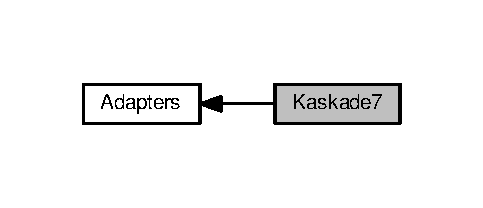
\includegraphics[width=337pt]{group__KaskadeGroup}
\end{center}
\end{figure}
\subsection*{Classes}
\begin{DoxyCompactItemize}
\item 
class \hyperlink{classSpacy_1_1Kaskade_1_1C1Operator}{Spacy\+::\+Kaskade\+::\+C1\+Operator$<$ Operator\+Definition $>$}
\begin{DoxyCompactList}\small\item\em Operator interface for Kaskade 7. Models a differentiable operator $A:X\rightarrow Y$. \end{DoxyCompactList}\item 
class \hyperlink{classSpacy_1_1Kaskade_1_1C2Functional}{Spacy\+::\+Kaskade\+::\+C2\+Functional$<$ Functional\+Definition $>$}
\begin{DoxyCompactList}\small\item\em Functional interface for Kaskade 7. Models a twice differentiable functional $f:X\rightarrow \mathbb{R}$. \end{DoxyCompactList}\item 
class \hyperlink{classSpacy_1_1Kaskade_1_1DirectSolver}{Spacy\+::\+Kaskade\+::\+Direct\+Solver$<$ Kaskade\+Operator, Ansatz\+Variable\+Description, Test\+Variable\+Description $>$}
\begin{DoxyCompactList}\small\item\em Direct solver interface for Kaskade 7. \end{DoxyCompactList}\item 
class \hyperlink{classSpacy_1_1Kaskade_1_1DynamicC1Operator}{Spacy\+::\+Kaskade\+::\+Dynamic\+C1\+Operator$<$ Operator\+Definition, Mass\+Definition $>$}
\begin{DoxyCompactList}\small\item\em Operator interface for Kaskade 7. Models a differentiable operator $A:X\rightarrow Y$. \end{DoxyCompactList}\item 
class \hyperlink{classSpacy_1_1Kaskade_1_1l2Product}{Spacy\+::\+Kaskade\+::l2\+Product$<$ Description $>$}
\begin{DoxyCompactList}\small\item\em Generic l2 scalar product for Kaskade7. Based on the implementation of the dual pairing. \end{DoxyCompactList}\item 
class \hyperlink{classSpacy_1_1Kaskade_1_1LinearOperator}{Spacy\+::\+Kaskade\+::\+Linear\+Operator$<$ Ansatz\+Variable\+Set\+Description, Test\+Variable\+Set\+Description $>$}
\begin{DoxyCompactList}\small\item\em Linear operator interface for operators in Kaskade 7. \end{DoxyCompactList}\item 
class \hyperlink{classSpacy_1_1Kaskade_1_1Operator}{Spacy\+::\+Kaskade\+::\+Operator$<$ Operator\+Definition $>$}
\begin{DoxyCompactList}\small\item\em Operator interface for Kaskade 7. Models an operator $A:X\rightarrow Y$. \end{DoxyCompactList}\item 
class \hyperlink{classSpacy_1_1Kaskade_1_1Vector}{Spacy\+::\+Kaskade\+::\+Vector$<$ Description $>$}
\begin{DoxyCompactList}\small\item\em Coefficient vector implementation for Kaskade 7 (single space). \end{DoxyCompactList}\item 
class \hyperlink{classSpacy_1_1Kaskade_1_1VectorCreator}{Spacy\+::\+Kaskade\+::\+Vector\+Creator$<$ Description $>$}
\begin{DoxyCompactList}\small\item\em Creator for vector space elements for Kaskade 7. \end{DoxyCompactList}\end{DoxyCompactItemize}
\subsection*{Functions}
\begin{DoxyCompactItemize}
\item 
{\footnotesize template$<$class Operator\+Definition $>$ }\\auto \hyperlink{group__KaskadeGroup_gae521d64422967ee3679b8e5bc26de996_gae521d64422967ee3679b8e5bc26de996}{Spacy\+::\+Kaskade\+::make\+C1\+Operator} (const Operator\+Definition \&f, const Vector\+Space \&domain, const Vector\+Space \&range, int rbegin=0, int rend=Operator\+Definition\+::\+Ansatz\+Vars\+::no\+Of\+Variables, int cbegin=0, int cend=Operator\+Definition\+::\+Test\+Vars\+::no\+Of\+Variables)
\begin{DoxyCompactList}\small\item\em Convenient generation of a differentiable operator $A: X\rightarrow Y$ from Kaskade 7. \end{DoxyCompactList}\item 
{\footnotesize template$<$class Operator\+Definition $>$ }\\auto \hyperlink{group__KaskadeGroup_ga8af78a452fabadde5f03fc4dc56face8_ga8af78a452fabadde5f03fc4dc56face8}{Spacy\+::\+Kaskade\+::make\+C1\+Operator} (const Operator\+Definition \&f, const Vector\+Space \&domain, int rbegin=0, int rend=Operator\+Definition\+::\+Ansatz\+Vars\+::no\+Of\+Variables, int cbegin=0, int cend=Operator\+Definition\+::\+Test\+Vars\+::no\+Of\+Variables)
\begin{DoxyCompactList}\small\item\em Convenient generation of a differentiable operator $A: X\rightarrow X^*$ from Kaskade 7. \end{DoxyCompactList}\item 
{\footnotesize template$<$class Functional\+Definition $>$ }\\auto \hyperlink{group__KaskadeGroup_gacef43eab636b05ddcfb7768041a2bc0e_gacef43eab636b05ddcfb7768041a2bc0e}{Spacy\+::\+Kaskade\+::make\+C2\+Functional} (const Functional\+Definition \&f, const Vector\+Space \&domain, int rbegin=0, int rend=Functional\+Definition\+::\+Ansatz\+Vars\+::no\+Of\+Variables, int cbegin=0, int cend=Functional\+Definition\+::\+Test\+Vars\+::no\+Of\+Variables)
\begin{DoxyCompactList}\small\item\em Convenient generation of a twice differentiable functional $f: X\rightarrow \mathbb{R}$ for Kaskade 7. \end{DoxyCompactList}\item 
{\footnotesize template$<$class Operator\+Definition $>$ }\\auto \hyperlink{group__KaskadeGroup_gac4502ad2f54b2c7d82e2a5d5790dc8b6_gac4502ad2f54b2c7d82e2a5d5790dc8b6}{Spacy\+::\+Kaskade\+::make\+Dynamic\+C1\+Operator} (const Operator\+Definition \&f, const Vector\+Space \&domain, const Vector\+Space \&range, int rbegin=0, int rend=Operator\+Definition\+::\+Ansatz\+Vars\+::no\+Of\+Variables, int cbegin=0, int cend=Operator\+Definition\+::\+Test\+Vars\+::no\+Of\+Variables)
\begin{DoxyCompactList}\small\item\em Convenient generation of a differentiable operator $A: X\rightarrow Y$ from Kaskade 7. \end{DoxyCompactList}\item 
{\footnotesize template$<$class Operator\+Definition $>$ }\\auto \hyperlink{group__KaskadeGroup_gacb385469fa2c1465b9ed8cbe6fabc13c_gacb385469fa2c1465b9ed8cbe6fabc13c}{Spacy\+::\+Kaskade\+::make\+Dynamic\+C1\+Operator} (const Operator\+Definition \&f, const Vector\+Space \&domain, int rbegin=0, int rend=Operator\+Definition\+::\+Ansatz\+Vars\+::no\+Of\+Variables, int cbegin=0, int cend=Operator\+Definition\+::\+Test\+Vars\+::no\+Of\+Variables)
\begin{DoxyCompactList}\small\item\em Convenient generation of a differentiable operator $A: X\rightarrow X^*$ from Kaskade 7. \end{DoxyCompactList}\item 
{\footnotesize template$<$class Ansatz\+Variable\+Set\+Description , class Test\+Variable\+Set\+Description , class Operator\+Impl $>$ }\\auto \hyperlink{group__KaskadeGroup_ga6bd8e1d7fdd3066ecd7ed14f0a239912_ga6bd8e1d7fdd3066ecd7ed14f0a239912}{Spacy\+::\+Kaskade\+::make\+Linear\+Operator} (const Operator\+Impl \&A, const Vector\+Space \&domain, const Vector\+Space \&range)
\begin{DoxyCompactList}\small\item\em Convenient generation of a linear operator for Kaskade 7. \end{DoxyCompactList}\item 
{\footnotesize template$<$class Operator\+Definition $>$ }\\auto \hyperlink{group__KaskadeGroup_ga0e8d7d2c51e429e22561ef813fc97589_ga0e8d7d2c51e429e22561ef813fc97589}{Spacy\+::\+Kaskade\+::make\+Operator} (const Operator\+Definition \&f, const Vector\+Space \&domain, const Vector\+Space \&range)
\begin{DoxyCompactList}\small\item\em Convenient generation of a differentiable operator $A: X\rightarrow Y$ from Kaskade 7. \end{DoxyCompactList}\item 
{\footnotesize template$<$class Operator\+Definition $>$ }\\auto \hyperlink{group__KaskadeGroup_ga3afbd00437ea7bdb406f3d9a1f375522_ga3afbd00437ea7bdb406f3d9a1f375522}{Spacy\+::\+Kaskade\+::make\+Operator} (const Operator\+Definition \&f, const Vector\+Space \&domain)
\begin{DoxyCompactList}\small\item\em Convenient generation of a differentiable operator $A: X\rightarrow X^*$ from Kaskade 7. \end{DoxyCompactList}\item 
\hypertarget{group__KaskadeGroup_ga2354f9e41ef04d4ea06b28b719668c96}{}{\footnotesize template$<$class Description $>$ }\\auto \hyperlink{group__KaskadeGroup_ga2354f9e41ef04d4ea06b28b719668c96}{Spacy\+::\+Kaskade\+::extract\+Spaces} (const Vector\+Space \&spaces)\label{group__KaskadeGroup_ga2354f9e41ef04d4ea06b28b719668c96}

\begin{DoxyCompactList}\small\item\em Extract boost\+::fusion\+::vector$<$ const Space0$\ast$, const Space1$\ast$, ... $>$ from spaces. \end{DoxyCompactList}\item 
{\footnotesize template$<$class Description $>$ }\\void \hyperlink{group__KaskadeGroup_gafbbd7e385eda54f651c45b1c074d7bf9_gafbbd7e385eda54f651c45b1c074d7bf9}{Spacy\+::\+Kaskade\+::copy} (const \+::\hyperlink{classSpacy_1_1Vector}{Spacy\+::\+Vector} \&x,\+::Kaskade\+::\+Variable\+Set$<$ Description $>$ \&y)
\begin{DoxyCompactList}\small\item\em Copy from \hyperlink{group__SpacyGroup_gafc144d2730ef87a67e54f8cd750b1f54_VectorAnchor}{\+:\+:Spacy\+:\+:Vector} to Kaskade\+::\+Variable\+Set. \end{DoxyCompactList}\item 
{\footnotesize template$<$class Description $>$ }\\void \hyperlink{group__KaskadeGroup_ga4d7422b0c155f9622e54b9d3503d82d8_ga4d7422b0c155f9622e54b9d3503d82d8}{Spacy\+::\+Kaskade\+::copy\+To\+Coefficient\+Vector} (const \+::\hyperlink{classSpacy_1_1Vector}{Spacy\+::\+Vector} \&x, typename Description\+::template Coefficient\+Vector\+Representation$<$$>$\+::type \&y)
\begin{DoxyCompactList}\small\item\em Copy from \hyperlink{group__SpacyGroup_gafc144d2730ef87a67e54f8cd750b1f54_VectorAnchor}{\+:\+:Spacy\+:\+:Vector} to coefficient vector of Kaskade 7. \end{DoxyCompactList}\item 
{\footnotesize template$<$class Description $>$ }\\void \hyperlink{group__KaskadeGroup_ga75249db31f75e23a474c4a9a5b792d67_ga75249db31f75e23a474c4a9a5b792d67}{Spacy\+::\+Kaskade\+::copy\+From\+Coefficient\+Vector} (const typename Description\+::template Coefficient\+Vector\+Representation$<$$>$\+::type \&x,\+::\hyperlink{classSpacy_1_1Vector}{Spacy\+::\+Vector} \&y)
\begin{DoxyCompactList}\small\item\em Copy coefficient vector of Kaskade 7 to \hyperlink{group__SpacyGroup_gafc144d2730ef87a67e54f8cd750b1f54_VectorAnchor}{\+:\+:Spacy\+:\+:Vector}. \end{DoxyCompactList}\item 
{\footnotesize template$<$class Description $>$ }\\auto \hyperlink{group__KaskadeGroup_ga04d45446864bbf87770d02eade7b64cf_ga04d45446864bbf87770d02eade7b64cf}{Spacy\+::\+Kaskade\+::make\+Hilbert\+Space} (const Description \&description)
\begin{DoxyCompactList}\small\item\em Create single space with hilbert space structure for Kaskade 7. \end{DoxyCompactList}\item 
{\footnotesize template$<$class Description $>$ }\\auto \hyperlink{group__KaskadeGroup_ga221db25c41371a2a823a6b569d735ef6_ga221db25c41371a2a823a6b569d735ef6}{Spacy\+::\+Kaskade\+::make\+Hilbert\+Space} (const Description \&description, const std\+::vector$<$ unsigned $>$ \&primal\+Ids, const std\+::vector$<$ unsigned $>$ \&dual\+Ids=\{\})
\begin{DoxyCompactList}\small\item\em Create product space with hilbert space structure for Kaskade 7. \end{DoxyCompactList}\end{DoxyCompactItemize}


\subsection{Detailed Description}
Vector spaces, functionals and operators for \href{http://www.zib.de/projects/kaskade7-finite-element-toolbox}{\tt Kaskade 7}. 



\subsection{Function Documentation}
\hypertarget{group__KaskadeGroup_gafbbd7e385eda54f651c45b1c074d7bf9_gafbbd7e385eda54f651c45b1c074d7bf9}{}\index{Vector Space for Kaskade 7@{Vector Space for Kaskade 7}!copy@{copy}}
\index{copy@{copy}!Vector Space for Kaskade 7@{Vector Space for Kaskade 7}}
\subsubsection[{copy}]{\setlength{\rightskip}{0pt plus 5cm}template$<$class Description $>$ void Spacy\+::\+Kaskade\+::copy (
\begin{DoxyParamCaption}
\item[{const \+::{\bf Spacy\+::\+Vector} \&}]{x, }
\item[{\+::Kaskade\+::\+Variable\+Set$<$ Description $>$ \&}]{y}
\end{DoxyParamCaption}
)}\label{group__KaskadeGroup_gafbbd7e385eda54f651c45b1c074d7bf9_gafbbd7e385eda54f651c45b1c074d7bf9}


Copy from \hyperlink{group__SpacyGroup_gafc144d2730ef87a67e54f8cd750b1f54_VectorAnchor}{\+:\+:Spacy\+:\+:Vector} to Kaskade\+::\+Variable\+Set. 

Takes into account product space structures. \hypertarget{group__KaskadeGroup_ga75249db31f75e23a474c4a9a5b792d67_ga75249db31f75e23a474c4a9a5b792d67}{}\index{Vector Space for Kaskade 7@{Vector Space for Kaskade 7}!copy\+From\+Coefficient\+Vector@{copy\+From\+Coefficient\+Vector}}
\index{copy\+From\+Coefficient\+Vector@{copy\+From\+Coefficient\+Vector}!Vector Space for Kaskade 7@{Vector Space for Kaskade 7}}
\subsubsection[{copy\+From\+Coefficient\+Vector}]{\setlength{\rightskip}{0pt plus 5cm}template$<$class Description $>$ void Spacy\+::\+Kaskade\+::copy\+From\+Coefficient\+Vector (
\begin{DoxyParamCaption}
\item[{const typename Description\+::template Coefficient\+Vector\+Representation$<$$>$\+::type \&}]{x, }
\item[{\+::{\bf Spacy\+::\+Vector} \&}]{y}
\end{DoxyParamCaption}
)}\label{group__KaskadeGroup_ga75249db31f75e23a474c4a9a5b792d67_ga75249db31f75e23a474c4a9a5b792d67}


Copy coefficient vector of Kaskade 7 to \hyperlink{group__SpacyGroup_gafc144d2730ef87a67e54f8cd750b1f54_VectorAnchor}{\+:\+:Spacy\+:\+:Vector}. 

Takes into account product space structures. \hypertarget{group__KaskadeGroup_ga4d7422b0c155f9622e54b9d3503d82d8_ga4d7422b0c155f9622e54b9d3503d82d8}{}\index{Vector Space for Kaskade 7@{Vector Space for Kaskade 7}!copy\+To\+Coefficient\+Vector@{copy\+To\+Coefficient\+Vector}}
\index{copy\+To\+Coefficient\+Vector@{copy\+To\+Coefficient\+Vector}!Vector Space for Kaskade 7@{Vector Space for Kaskade 7}}
\subsubsection[{copy\+To\+Coefficient\+Vector}]{\setlength{\rightskip}{0pt plus 5cm}template$<$class Description $>$ void Spacy\+::\+Kaskade\+::copy\+To\+Coefficient\+Vector (
\begin{DoxyParamCaption}
\item[{const \+::{\bf Spacy\+::\+Vector} \&}]{x, }
\item[{typename Description\+::template Coefficient\+Vector\+Representation$<$$>$\+::type \&}]{y}
\end{DoxyParamCaption}
)}\label{group__KaskadeGroup_ga4d7422b0c155f9622e54b9d3503d82d8_ga4d7422b0c155f9622e54b9d3503d82d8}


Copy from \hyperlink{group__SpacyGroup_gafc144d2730ef87a67e54f8cd750b1f54_VectorAnchor}{\+:\+:Spacy\+:\+:Vector} to coefficient vector of Kaskade 7. 

Takes into account product space structures. \hypertarget{group__KaskadeGroup_gae521d64422967ee3679b8e5bc26de996_gae521d64422967ee3679b8e5bc26de996}{}\index{Vector Space for Kaskade 7@{Vector Space for Kaskade 7}!make\+C1\+Operator@{make\+C1\+Operator}}
\index{make\+C1\+Operator@{make\+C1\+Operator}!Vector Space for Kaskade 7@{Vector Space for Kaskade 7}}
\subsubsection[{make\+C1\+Operator}]{\setlength{\rightskip}{0pt plus 5cm}template$<$class Operator\+Definition $>$ auto Spacy\+::\+Kaskade\+::make\+C1\+Operator (
\begin{DoxyParamCaption}
\item[{const Operator\+Definition \&}]{f, }
\item[{const {\bf Vector\+Space} \&}]{domain, }
\item[{const {\bf Vector\+Space} \&}]{range, }
\item[{int}]{rbegin = {\ttfamily 0}, }
\item[{int}]{rend = {\ttfamily OperatorDefinition\+:\+:AnsatzVars\+:\+:noOfVariables}, }
\item[{int}]{cbegin = {\ttfamily 0}, }
\item[{int}]{cend = {\ttfamily OperatorDefinition\+:\+:TestVars\+:\+:noOfVariables}}
\end{DoxyParamCaption}
)}\label{group__KaskadeGroup_gae521d64422967ee3679b8e5bc26de996_gae521d64422967ee3679b8e5bc26de996}


Convenient generation of a differentiable operator $A: X\rightarrow Y$ from Kaskade 7. 


\begin{DoxyParams}{Parameters}
{\em f} & operator definition from Kaskade 7 \\
\hline
{\em domain} & domain space $X$ \\
\hline
{\em range} & range space $Y$ \\
\hline
{\em rbegin} & first row to be considered in the definition of A \\
\hline
{\em rend} & one after the last row to be considered in the definition of A \\
\hline
{\em cbegin} & first column to be considered in the definition of A \\
\hline
{\em cend} & one after the last column to be considered in the definition of A \\
\hline
\end{DoxyParams}
\begin{DoxyReturn}{Returns}
\hyperlink{classSpacy_1_1Kaskade_1_1C1Operator}{\+:\+:Spacy\+:\+:Kaskade\+:\+:C1\+Operator$<$Operator\+Definition$>$( A , domain , range , rbegin , rend , cbegin , cend )}
\end{DoxyReturn}
The optional parameters rbegin, rend, cbegin and cend can be used to define operators that correspond to parts of a system of equation. \hypertarget{group__KaskadeGroup_ga8af78a452fabadde5f03fc4dc56face8_ga8af78a452fabadde5f03fc4dc56face8}{}\index{Vector Space for Kaskade 7@{Vector Space for Kaskade 7}!make\+C1\+Operator@{make\+C1\+Operator}}
\index{make\+C1\+Operator@{make\+C1\+Operator}!Vector Space for Kaskade 7@{Vector Space for Kaskade 7}}
\subsubsection[{make\+C1\+Operator}]{\setlength{\rightskip}{0pt plus 5cm}template$<$class Operator\+Definition $>$ auto Spacy\+::\+Kaskade\+::make\+C1\+Operator (
\begin{DoxyParamCaption}
\item[{const Operator\+Definition \&}]{f, }
\item[{const {\bf Vector\+Space} \&}]{domain, }
\item[{int}]{rbegin = {\ttfamily 0}, }
\item[{int}]{rend = {\ttfamily OperatorDefinition\+:\+:AnsatzVars\+:\+:noOfVariables}, }
\item[{int}]{cbegin = {\ttfamily 0}, }
\item[{int}]{cend = {\ttfamily OperatorDefinition\+:\+:TestVars\+:\+:noOfVariables}}
\end{DoxyParamCaption}
)}\label{group__KaskadeGroup_ga8af78a452fabadde5f03fc4dc56face8_ga8af78a452fabadde5f03fc4dc56face8}


Convenient generation of a differentiable operator $A: X\rightarrow X^*$ from Kaskade 7. 


\begin{DoxyParams}{Parameters}
{\em f} & operator definition from Kaskade 7 \\
\hline
{\em domain} & domain space $X$ \\
\hline
{\em rbegin} & first row to be considered in the definition of A \\
\hline
{\em rend} & one after the last row to be considered in the definition of A \\
\hline
{\em cbegin} & first column to be considered in the definition of A \\
\hline
{\em cend} & one after the last column to be considered in the definition of A \\
\hline
\end{DoxyParams}
\begin{DoxyReturn}{Returns}
\hyperlink{classSpacy_1_1Kaskade_1_1C1Operator}{\+:\+:Spacy\+:\+:Kaskade\+:\+:C1\+Operator$<$Operator\+Definition$>$( A , domain , range , rbegin , rend , cbegin , cend )}
\end{DoxyReturn}
The optional parameters rbegin, rend, cbegin and cend can be used to define operators that correspond to parts of a system of equation. \hypertarget{group__KaskadeGroup_gacef43eab636b05ddcfb7768041a2bc0e_gacef43eab636b05ddcfb7768041a2bc0e}{}\index{Vector Space for Kaskade 7@{Vector Space for Kaskade 7}!make\+C2\+Functional@{make\+C2\+Functional}}
\index{make\+C2\+Functional@{make\+C2\+Functional}!Vector Space for Kaskade 7@{Vector Space for Kaskade 7}}
\subsubsection[{make\+C2\+Functional}]{\setlength{\rightskip}{0pt plus 5cm}template$<$class Functional\+Definition $>$ auto Spacy\+::\+Kaskade\+::make\+C2\+Functional (
\begin{DoxyParamCaption}
\item[{const Functional\+Definition \&}]{f, }
\item[{const {\bf Vector\+Space} \&}]{domain, }
\item[{int}]{rbegin = {\ttfamily 0}, }
\item[{int}]{rend = {\ttfamily FunctionalDefinition\+:\+:AnsatzVars\+:\+:noOfVariables}, }
\item[{int}]{cbegin = {\ttfamily 0}, }
\item[{int}]{cend = {\ttfamily FunctionalDefinition\+:\+:TestVars\+:\+:noOfVariables}}
\end{DoxyParamCaption}
)}\label{group__KaskadeGroup_gacef43eab636b05ddcfb7768041a2bc0e_gacef43eab636b05ddcfb7768041a2bc0e}


Convenient generation of a twice differentiable functional $f: X\rightarrow \mathbb{R}$ for Kaskade 7. 


\begin{DoxyParams}{Parameters}
{\em f} & operator definition from Kaskade 7 \\
\hline
{\em domain} & domain space \\
\hline
{\em rbegin} & first row to be considered in the definition of f \\
\hline
{\em rend} & one after the last row to be considered in the definition of f \\
\hline
{\em cbegin} & first column to be considered in the definition of f \\
\hline
{\em cend} & one after the last column to be considered in the definition of f \\
\hline
\end{DoxyParams}
\begin{DoxyReturn}{Returns}
\hyperlink{classSpacy_1_1Kaskade_1_1C2Functional}{\+:\+:Spacy\+:\+:Kaskade\+:\+:C2\+Functional$<$Functional\+Definition$>$( f, domain, rbegin, rend, cbegin, cend )}
\end{DoxyReturn}
The optional parameters rbegin, rend, cbegin and cend can be used to define operators that correspond to parts of a system of equation. \hypertarget{group__KaskadeGroup_gac4502ad2f54b2c7d82e2a5d5790dc8b6_gac4502ad2f54b2c7d82e2a5d5790dc8b6}{}\index{Vector Space for Kaskade 7@{Vector Space for Kaskade 7}!make\+Dynamic\+C1\+Operator@{make\+Dynamic\+C1\+Operator}}
\index{make\+Dynamic\+C1\+Operator@{make\+Dynamic\+C1\+Operator}!Vector Space for Kaskade 7@{Vector Space for Kaskade 7}}
\subsubsection[{make\+Dynamic\+C1\+Operator}]{\setlength{\rightskip}{0pt plus 5cm}template$<$class Operator\+Definition $>$ auto Spacy\+::\+Kaskade\+::make\+Dynamic\+C1\+Operator (
\begin{DoxyParamCaption}
\item[{const Operator\+Definition \&}]{f, }
\item[{const {\bf Vector\+Space} \&}]{domain, }
\item[{const {\bf Vector\+Space} \&}]{range, }
\item[{int}]{rbegin = {\ttfamily 0}, }
\item[{int}]{rend = {\ttfamily OperatorDefinition\+:\+:AnsatzVars\+:\+:noOfVariables}, }
\item[{int}]{cbegin = {\ttfamily 0}, }
\item[{int}]{cend = {\ttfamily OperatorDefinition\+:\+:TestVars\+:\+:noOfVariables}}
\end{DoxyParamCaption}
)}\label{group__KaskadeGroup_gac4502ad2f54b2c7d82e2a5d5790dc8b6_gac4502ad2f54b2c7d82e2a5d5790dc8b6}


Convenient generation of a differentiable operator $A: X\rightarrow Y$ from Kaskade 7. 


\begin{DoxyParams}{Parameters}
{\em f} & operator definition from Kaskade 7 \\
\hline
{\em domain} & domain space $X$ \\
\hline
{\em range} & range space $Y$ \\
\hline
{\em rbegin} & first row to be considered in the definition of A \\
\hline
{\em rend} & one after the last row to be considered in the definition of A \\
\hline
{\em cbegin} & first column to be considered in the definition of A \\
\hline
{\em cend} & one after the last column to be considered in the definition of A \\
\hline
\end{DoxyParams}
\begin{DoxyReturn}{Returns}
\hyperlink{classSpacy_1_1Kaskade_1_1DynamicC1Operator}{\+:\+:Spacy\+:\+:Kaskade\+:\+:Dynamic\+C1\+Operator$<$Operator\+Definition$>$( A , domain , range , rbegin , rend , cbegin , cend )}
\end{DoxyReturn}
The optional parameters rbegin, rend, cbegin and cend can be used to define operators that correspond to parts of a system of equation. \hypertarget{group__KaskadeGroup_gacb385469fa2c1465b9ed8cbe6fabc13c_gacb385469fa2c1465b9ed8cbe6fabc13c}{}\index{Vector Space for Kaskade 7@{Vector Space for Kaskade 7}!make\+Dynamic\+C1\+Operator@{make\+Dynamic\+C1\+Operator}}
\index{make\+Dynamic\+C1\+Operator@{make\+Dynamic\+C1\+Operator}!Vector Space for Kaskade 7@{Vector Space for Kaskade 7}}
\subsubsection[{make\+Dynamic\+C1\+Operator}]{\setlength{\rightskip}{0pt plus 5cm}template$<$class Operator\+Definition $>$ auto Spacy\+::\+Kaskade\+::make\+Dynamic\+C1\+Operator (
\begin{DoxyParamCaption}
\item[{const Operator\+Definition \&}]{f, }
\item[{const {\bf Vector\+Space} \&}]{domain, }
\item[{int}]{rbegin = {\ttfamily 0}, }
\item[{int}]{rend = {\ttfamily OperatorDefinition\+:\+:AnsatzVars\+:\+:noOfVariables}, }
\item[{int}]{cbegin = {\ttfamily 0}, }
\item[{int}]{cend = {\ttfamily OperatorDefinition\+:\+:TestVars\+:\+:noOfVariables}}
\end{DoxyParamCaption}
)}\label{group__KaskadeGroup_gacb385469fa2c1465b9ed8cbe6fabc13c_gacb385469fa2c1465b9ed8cbe6fabc13c}


Convenient generation of a differentiable operator $A: X\rightarrow X^*$ from Kaskade 7. 


\begin{DoxyParams}{Parameters}
{\em f} & operator definition from Kaskade 7 \\
\hline
{\em domain} & domain space $X$ \\
\hline
{\em rbegin} & first row to be considered in the definition of A \\
\hline
{\em rend} & one after the last row to be considered in the definition of A \\
\hline
{\em cbegin} & first column to be considered in the definition of A \\
\hline
{\em cend} & one after the last column to be considered in the definition of A \\
\hline
\end{DoxyParams}
\begin{DoxyReturn}{Returns}
\hyperlink{classSpacy_1_1Kaskade_1_1DynamicC1Operator}{\+:\+:Spacy\+:\+:Kaskade\+:\+:Dynamic\+C1\+Operator$<$Operator\+Definition$>$( A , domain , range , rbegin , rend , cbegin , cend )}
\end{DoxyReturn}
The optional parameters rbegin, rend, cbegin and cend can be used to define operators that correspond to parts of a system of equation. \hypertarget{group__KaskadeGroup_ga04d45446864bbf87770d02eade7b64cf_ga04d45446864bbf87770d02eade7b64cf}{}\index{Vector Space for Kaskade 7@{Vector Space for Kaskade 7}!make\+Hilbert\+Space@{make\+Hilbert\+Space}}
\index{make\+Hilbert\+Space@{make\+Hilbert\+Space}!Vector Space for Kaskade 7@{Vector Space for Kaskade 7}}
\subsubsection[{make\+Hilbert\+Space}]{\setlength{\rightskip}{0pt plus 5cm}template$<$class Description $>$ auto Spacy\+::\+Kaskade\+::make\+Hilbert\+Space (
\begin{DoxyParamCaption}
\item[{const Description \&}]{description}
\end{DoxyParamCaption}
)}\label{group__KaskadeGroup_ga04d45446864bbf87770d02eade7b64cf_ga04d45446864bbf87770d02eade7b64cf}


Create single space with hilbert space structure for Kaskade 7. 


\begin{DoxyParams}{Parameters}
{\em space} & single Kaskade 7 function space (no product space) \\
\hline
\end{DoxyParams}
\hypertarget{group__KaskadeGroup_ga221db25c41371a2a823a6b569d735ef6_ga221db25c41371a2a823a6b569d735ef6}{}\index{Vector Space for Kaskade 7@{Vector Space for Kaskade 7}!make\+Hilbert\+Space@{make\+Hilbert\+Space}}
\index{make\+Hilbert\+Space@{make\+Hilbert\+Space}!Vector Space for Kaskade 7@{Vector Space for Kaskade 7}}
\subsubsection[{make\+Hilbert\+Space}]{\setlength{\rightskip}{0pt plus 5cm}template$<$class Description $>$ auto Spacy\+::\+Kaskade\+::make\+Hilbert\+Space (
\begin{DoxyParamCaption}
\item[{const Description \&}]{description, }
\item[{const std\+::vector$<$ unsigned $>$ \&}]{primal\+Ids, }
\item[{const std\+::vector$<$ unsigned $>$ \&}]{dual\+Ids = {\ttfamily \{\}}}
\end{DoxyParamCaption}
)}\label{group__KaskadeGroup_ga221db25c41371a2a823a6b569d735ef6_ga221db25c41371a2a823a6b569d735ef6}


Create product space with hilbert space structure for Kaskade 7. 


\begin{DoxyParams}{Parameters}
{\em spaces} & boost fusion forward sequence of const pointers to Kaskade 7 function spaces \\
\hline
{\em primal\+Ids} & ids of primal variables \\
\hline
{\em dual\+Ids} & ids of dual variables \\
\hline
\end{DoxyParams}
\hypertarget{group__KaskadeGroup_ga6bd8e1d7fdd3066ecd7ed14f0a239912_ga6bd8e1d7fdd3066ecd7ed14f0a239912}{}\index{Vector Space for Kaskade 7@{Vector Space for Kaskade 7}!make\+Linear\+Operator@{make\+Linear\+Operator}}
\index{make\+Linear\+Operator@{make\+Linear\+Operator}!Vector Space for Kaskade 7@{Vector Space for Kaskade 7}}
\subsubsection[{make\+Linear\+Operator}]{\setlength{\rightskip}{0pt plus 5cm}template$<$class Ansatz\+Variable\+Set\+Description , class Test\+Variable\+Set\+Description , class Operator\+Impl $>$ auto Spacy\+::\+Kaskade\+::make\+Linear\+Operator (
\begin{DoxyParamCaption}
\item[{const Operator\+Impl \&}]{A, }
\item[{const {\bf Vector\+Space} \&}]{domain, }
\item[{const {\bf Vector\+Space} \&}]{range}
\end{DoxyParamCaption}
)}\label{group__KaskadeGroup_ga6bd8e1d7fdd3066ecd7ed14f0a239912_ga6bd8e1d7fdd3066ecd7ed14f0a239912}


Convenient generation of a linear operator for Kaskade 7. 


\begin{DoxyParams}{Parameters}
{\em A} & operator from Kaskade 7 \\
\hline
{\em domain} & domain space \\
\hline
{\em range} & range space \\
\hline
\end{DoxyParams}

\begin{DoxyTemplParams}{Template Parameters}
{\em Operator\+Impl} & Kaskade 7 operator, i.\+e. Kaskade\+::\+Assembled\+Galerkin\+Operator or Kaskade\+::\+Matrix\+Represented\+Operator. \\
\hline
{\em Ansatz\+Variable\+Set\+Description} & Kaskade\+::\+Variable\+Set\+Description for ansatz variables \\
\hline
{\em Test\+Variable\+Set\+Description} & Kaskade\+::\+Variable\+Set\+Description for test variables \\
\hline
\end{DoxyTemplParams}
\begin{DoxyReturn}{Returns}
Linear\+Operator$<$\+Operator\+Impl, Ansatz\+Variable\+Set\+Description, Test\+Variable\+Set\+Description$>$( A , domain , range ) 
\end{DoxyReturn}
\hypertarget{group__KaskadeGroup_ga0e8d7d2c51e429e22561ef813fc97589_ga0e8d7d2c51e429e22561ef813fc97589}{}\index{Vector Space for Kaskade 7@{Vector Space for Kaskade 7}!make\+Operator@{make\+Operator}}
\index{make\+Operator@{make\+Operator}!Vector Space for Kaskade 7@{Vector Space for Kaskade 7}}
\subsubsection[{make\+Operator}]{\setlength{\rightskip}{0pt plus 5cm}template$<$class Operator\+Definition $>$ auto Spacy\+::\+Kaskade\+::make\+Operator (
\begin{DoxyParamCaption}
\item[{const Operator\+Definition \&}]{f, }
\item[{const {\bf Vector\+Space} \&}]{domain, }
\item[{const {\bf Vector\+Space} \&}]{range}
\end{DoxyParamCaption}
)}\label{group__KaskadeGroup_ga0e8d7d2c51e429e22561ef813fc97589_ga0e8d7d2c51e429e22561ef813fc97589}


Convenient generation of a differentiable operator $A: X\rightarrow Y$ from Kaskade 7. 


\begin{DoxyParams}{Parameters}
{\em f} & operator definition from Kaskade 7 \\
\hline
{\em domain} & domain space $X$ \\
\hline
{\em range} & range space $Y$ \\
\hline
\end{DoxyParams}
\begin{DoxyReturn}{Returns}
\hyperlink{classSpacy_1_1Kaskade_1_1Operator}{\+:\+:Spacy\+:\+:Kaskade\+:\+:Operator$<$Operator\+Definition$>$( A , domain , range )} 
\end{DoxyReturn}
\hypertarget{group__KaskadeGroup_ga3afbd00437ea7bdb406f3d9a1f375522_ga3afbd00437ea7bdb406f3d9a1f375522}{}\index{Vector Space for Kaskade 7@{Vector Space for Kaskade 7}!make\+Operator@{make\+Operator}}
\index{make\+Operator@{make\+Operator}!Vector Space for Kaskade 7@{Vector Space for Kaskade 7}}
\subsubsection[{make\+Operator}]{\setlength{\rightskip}{0pt plus 5cm}template$<$class Operator\+Definition $>$ auto Spacy\+::\+Kaskade\+::make\+Operator (
\begin{DoxyParamCaption}
\item[{const Operator\+Definition \&}]{f, }
\item[{const {\bf Vector\+Space} \&}]{domain}
\end{DoxyParamCaption}
)}\label{group__KaskadeGroup_ga3afbd00437ea7bdb406f3d9a1f375522_ga3afbd00437ea7bdb406f3d9a1f375522}


Convenient generation of a differentiable operator $A: X\rightarrow X^*$ from Kaskade 7. 


\begin{DoxyParams}{Parameters}
{\em f} & operator definition from Kaskade 7 \\
\hline
{\em domain} & domain space $X$ \\
\hline
\end{DoxyParams}
\begin{DoxyReturn}{Returns}
\hyperlink{classSpacy_1_1Kaskade_1_1Operator}{\+:\+:Spacy\+:\+:Kaskade\+:\+:Operator$<$Operator\+Definition$>$( A , domain , range )} 
\end{DoxyReturn}

\hypertarget{group__MixinGroup}{}\section{Mixins}
\label{group__MixinGroup}\index{Mixins@{Mixins}}


Components that are frequently used and can be added to your classes via (multiple) inheritance.  


\subsection*{Classes}
\begin{DoxyCompactItemize}
\item 
class \hyperlink{classSpacy_1_1Mixin_1_1AbsoluteAccuracy}{Spacy\+::\+Mixin\+::\+Absolute\+Accuracy}
\begin{DoxyCompactList}\small\item\em Mixin class for absolute accuracy. \end{DoxyCompactList}\item 
class \hyperlink{classSpacy_1_1Mixin_1_1AdjointIndex}{Spacy\+::\+Mixin\+::\+Adjoint\+Index}
\begin{DoxyCompactList}\small\item\em Mixin class for index of the adjoint variable. \end{DoxyCompactList}\item 
class \hyperlink{classSpacy_1_1Mixin_1_1ContractionRate}{Spacy\+::\+Mixin\+::\+Contraction\+Rate}
\begin{DoxyCompactList}\small\item\em Mixin class for contraction rates. \end{DoxyCompactList}\item 
class \hyperlink{classSpacy_1_1Mixin_1_1ControlIndex}{Spacy\+::\+Mixin\+::\+Control\+Index}
\begin{DoxyCompactList}\small\item\em Mixin class for index of the control variable. \end{DoxyCompactList}\item 
class \hyperlink{classSpacy_1_1Mixin_1_1DampingAccuracy}{Spacy\+::\+Mixin\+::\+Damping\+Accuracy}
\begin{DoxyCompactList}\small\item\em Mixin class for the accuracy of damping factors. \end{DoxyCompactList}\item 
class \hyperlink{classSpacy_1_1Mixin_1_1DecreaseCondition}{Spacy\+::\+Mixin\+::\+Decrease\+Condition}
\begin{DoxyCompactList}\small\item\em Mixin class for accepting local models $m$ of nonlinear optimization problems $\min f(x)$. \end{DoxyCompactList}\item 
class \hyperlink{classSpacy_1_1Mixin_1_1Eps}{Spacy\+::\+Mixin\+::\+Eps}
\begin{DoxyCompactList}\small\item\em Mixin class for maximal attainable accuracy $\varepsilon$. \end{DoxyCompactList}\item 
class \hyperlink{classSpacy_1_1Mixin_1_1Impl}{Spacy\+::\+Mixin\+::\+Impl$<$ Type $>$}
\begin{DoxyCompactList}\small\item\em Stores an object of type Type and provides access via member function \hyperlink{classSpacy_1_1Mixin_1_1Impl_a5e61399bae41338a87e701b24b13f52a}{impl()}. \end{DoxyCompactList}\item 
class \hyperlink{classSpacy_1_1Mixin_1_1Impl_3_01const_01Type_01_6_01_4}{Spacy\+::\+Mixin\+::\+Impl$<$ const Type \& $>$}
\begin{DoxyCompactList}\small\item\em Stores an object of type Type by const reference and provides access via member function \hyperlink{classSpacy_1_1Mixin_1_1Impl_3_01const_01Type_01_6_01_4_a5999a2a31217f4d4e5a0354f0bd14f66}{impl()}. \end{DoxyCompactList}\item 
class \hyperlink{classSpacy_1_1Mixin_1_1UniqueImpl}{Spacy\+::\+Mixin\+::\+Unique\+Impl$<$ Type $>$}
\begin{DoxyCompactList}\small\item\em Stores an object of type Type as unique pointer and provides access via member function \hyperlink{classSpacy_1_1Mixin_1_1UniqueImpl_ae183ae8b045db161111f761a32703547}{impl()}. \end{DoxyCompactList}\item 
class \hyperlink{classSpacy_1_1Mixin_1_1CopyingUniqueImpl}{Spacy\+::\+Mixin\+::\+Copying\+Unique\+Impl$<$ Type $>$}
\begin{DoxyCompactList}\small\item\em Stores an object of type Type as unique pointer and provides access via member function \hyperlink{classSpacy_1_1Mixin_1_1CopyingUniqueImpl_ab7cc202fd000ba1753ef8596c09dc803}{impl()}. \end{DoxyCompactList}\item 
class \hyperlink{classSpacy_1_1Mixin_1_1SharedImpl}{Spacy\+::\+Mixin\+::\+Shared\+Impl$<$ Type $>$}
\begin{DoxyCompactList}\small\item\em Stores an object of type Type as shared pointer and provides access via member function \hyperlink{classSpacy_1_1Mixin_1_1SharedImpl_a4bed4faca68901d0dd463c4234fb2fe6}{impl()}. \end{DoxyCompactList}\item 
class \hyperlink{classSpacy_1_1Mixin_1_1NonOwningPImpl}{Spacy\+::\+Mixin\+::\+Non\+Owning\+P\+Impl$<$ Type $>$}
\begin{DoxyCompactList}\small\item\em Stores an object of type Type as (non-\/owning) raw pointer and provides access via member function \hyperlink{classSpacy_1_1Mixin_1_1NonOwningPImpl_aeeb3e0a5f6fd8f22633040dcf94355f9}{impl()}. \end{DoxyCompactList}\item 
class \hyperlink{classSpacy_1_1Mixin_1_1IterativeRefinements}{Spacy\+::\+Mixin\+::\+Iterative\+Refinements}
\begin{DoxyCompactList}\small\item\em Mixin class for iterative refinements. \end{DoxyCompactList}\item 
class \hyperlink{classSpacy_1_1Mixin_1_1MaxSteps}{Spacy\+::\+Mixin\+::\+Max\+Steps}
\begin{DoxyCompactList}\small\item\em Mixin class for maximal number of steps/iterations. \end{DoxyCompactList}\item 
class \hyperlink{classSpacy_1_1Mixin_1_1MinimalAccuracy}{Spacy\+::\+Mixin\+::\+Minimal\+Accuracy}
\begin{DoxyCompactList}\small\item\em Mixin class for minimal accuracy. \end{DoxyCompactList}\item 
class \hyperlink{classSpacy_1_1Mixin_1_1NumberOfThreads}{Spacy\+::\+Mixin\+::\+Number\+Of\+Threads}
\begin{DoxyCompactList}\small\item\em Mixin class for number of threads \end{DoxyCompactList}\item 
class \hyperlink{classSpacy_1_1Mixin_1_1PrimalDualSwitch}{Spacy\+::\+Mixin\+::\+Primal\+Dual\+Switch}
\begin{DoxyCompactList}\small\item\em Mixin class for separating primal and dual variables. \end{DoxyCompactList}\item 
class \hyperlink{classSpacy_1_1Mixin_1_1RegularityTest}{Spacy\+::\+Mixin\+::\+Regularity\+Test}
\begin{DoxyCompactList}\small\item\em Mixin class for maximal number of steps/iterations. \end{DoxyCompactList}\item 
class \hyperlink{classSpacy_1_1Mixin_1_1RelativeAccuracy}{Spacy\+::\+Mixin\+::\+Relative\+Accuracy}
\begin{DoxyCompactList}\small\item\em Mixin class for relative accuracy. \end{DoxyCompactList}\item 
class \hyperlink{classSpacy_1_1Mixin_1_1StateIndex}{Spacy\+::\+Mixin\+::\+State\+Index}
\begin{DoxyCompactList}\small\item\em Mixin class for index of state variable. \end{DoxyCompactList}\item 
class \hyperlink{classSpacy_1_1Mixin_1_1Timer}{Spacy\+::\+Mixin\+::\+Timer$<$ Unit $>$}
\begin{DoxyCompactList}\small\item\em Mixin class providing a simple timer. \end{DoxyCompactList}\item 
class \hyperlink{classSpacy_1_1Mixin_1_1Verbosity}{Spacy\+::\+Mixin\+::\+Verbosity}
\begin{DoxyCompactList}\small\item\em Mixin class for verbosity. \end{DoxyCompactList}\end{DoxyCompactItemize}
\subsection*{Typedefs}
\begin{DoxyCompactItemize}
\item 
\hypertarget{group__MixinGroup_ga3289264a84ff7bc4942d07318a22bfd7}{}{\footnotesize template$<$class Type $>$ }\\using \hyperlink{group__MixinGroup_ga3289264a84ff7bc4942d07318a22bfd7}{Spacy\+::\+Mixin\+::\+C\+Ref\+Impl} = Impl$<$ const Type \& $>$\label{group__MixinGroup_ga3289264a84ff7bc4942d07318a22bfd7}

\begin{DoxyCompactList}\small\item\em Stores an object of type Type by const reference and provides access via member function impl(). \end{DoxyCompactList}\end{DoxyCompactItemize}


\subsection{Detailed Description}
Components that are frequently used and can be added to your classes via (multiple) inheritance. 

Among the mixin components are
\begin{DoxyItemize}
\item components for different accuracy requirements (Mixin\+::\+Relative\+Accuracy, Mixin\+::\+Absolute\+Accuracy, Mixin\+::\+Minimal\+Accuracy, Mixin\+::\+Damping\+Accuracy)
\item a component for the maximal attainable accuracy (Mixin\+::\+Eps)
\item a component for the maximal number of steps/iterations (Mixin\+::\+Max\+Steps)
\item components for elementary algorithmic decisions (Mixin\+::\+Contraction\+Rate, Mixin\+::\+Decrease\+Condition, Mixin\+::\+Regularity\+Test)
\item indices for variables in optimization and optimal control problems ... 
\end{DoxyItemize}
\hypertarget{group__ExceptionGroup}{}\section{Exceptions}
\label{group__ExceptionGroup}\index{Exceptions@{Exceptions}}


Some simple exceptions.  


\subsection*{Classes}
\begin{DoxyCompactItemize}
\item 
class \hyperlink{classSpacy_1_1CallOfUndefinedFunctionException}{Spacy\+::\+Call\+Of\+Undefined\+Function\+Exception}
\begin{DoxyCompactList}\small\item\em Exception to be thrown if a virtual function is not implemented. \end{DoxyCompactList}\item 
class \hyperlink{classSpacy_1_1GenericException}{Spacy\+::\+Generic\+Exception}
\begin{DoxyCompactList}\small\item\em A generic exception class that serves as base for all exceptions in this library. \end{DoxyCompactList}\item 
class \hyperlink{classSpacy_1_1IncompatibleSpaceException}{Spacy\+::\+Incompatible\+Space\+Exception}
\begin{DoxyCompactList}\small\item\em Exception to be thrown when encountering incompatible spaces. \end{DoxyCompactList}\item 
class \hyperlink{classSpacy_1_1InvalidArgumentException}{Spacy\+::\+Invalid\+Argument\+Exception}
\begin{DoxyCompactList}\small\item\em Exception to be thrown on invalid arguments. \end{DoxyCompactList}\item 
class \hyperlink{classSpacy_1_1RegularityTestFailedException}{Spacy\+::\+Regularity\+Test\+Failed\+Exception}
\begin{DoxyCompactList}\small\item\em Exception to be thrown if regularity test fails. \end{DoxyCompactList}\item 
class \hyperlink{classSpacy_1_1SingularOperatorException}{Spacy\+::\+Singular\+Operator\+Exception}
\begin{DoxyCompactList}\small\item\em Exception to be thrown if singular operators are inverted. \end{DoxyCompactList}\end{DoxyCompactItemize}


\subsection{Detailed Description}
Some simple exceptions. 

\begin{DoxyRefDesc}{Todo}
\item[\hyperlink{todo__todo000001}{Todo}]improve \end{DoxyRefDesc}

\hypertarget{group__AlgorithmGroup}{}\section{Algorithms}
\label{group__AlgorithmGroup}\index{Algorithms@{Algorithms}}


Contains different algorithms that can be formulated in vector spaces.  


Collaboration diagram for Algorithms\+:\nopagebreak
\begin{figure}[H]
\begin{center}
\leavevmode
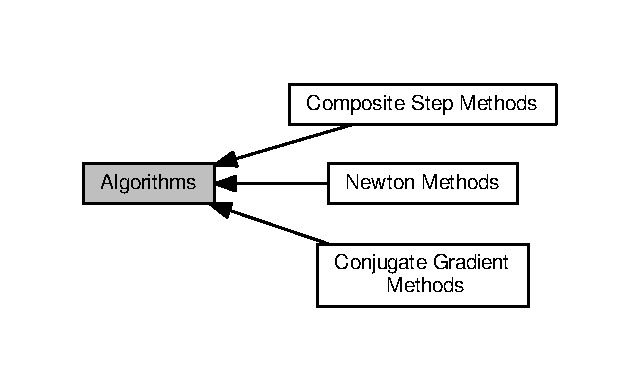
\includegraphics[width=307pt]{group__AlgorithmGroup}
\end{center}
\end{figure}
\subsection*{Modules}
\begin{DoxyCompactItemize}
\item 
\hyperlink{group__NewtonGroup}{Newton Methods}
\begin{DoxyCompactList}\small\item\em Newton methods, largely following \cite{Deuflhard2004}. \end{DoxyCompactList}\item 
\hyperlink{group__CGGroup}{Conjugate Gradient Methods}
\begin{DoxyCompactList}\small\item\em Conjugate gradient methods for convex and nonconvex problems (C\+G, Truncated C\+G, Regularized C\+G and Truncated Regularized C\+G). \end{DoxyCompactList}\item 
\hyperlink{group__CSGroup}{Composite Step Methods}
\begin{DoxyCompactList}\small\item\em Contains the affine covariant composite step method of \cite{Lubkoll2015}, \cite{Lubkoll2015a}. \end{DoxyCompactList}\end{DoxyCompactItemize}


\subsection{Detailed Description}
Contains different algorithms that can be formulated in vector spaces. 

Contains different variants of conjugate gradient methods for convex and nonconvex problems, different newton methods and an affine covariant composite step method. 
\hypertarget{group__NewtonGroup}{}\section{Newton Methods}
\label{group__NewtonGroup}\index{Newton Methods@{Newton Methods}}


Newton methods, largely following \cite{Deuflhard2004}.  


Collaboration diagram for Newton Methods\+:\nopagebreak
\begin{figure}[H]
\begin{center}
\leavevmode
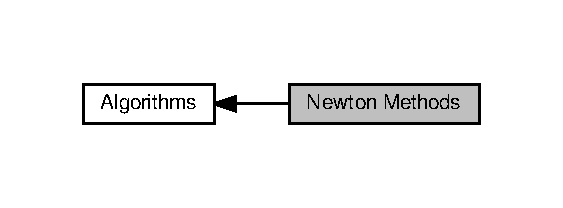
\includegraphics[width=270pt]{group__NewtonGroup}
\end{center}
\end{figure}
\subsection*{Classes}
\begin{DoxyCompactItemize}
\item 
class \hyperlink{classSpacy_1_1Newton_1_1Damping_1_1AffineCovariant}{Spacy\+::\+Newton\+::\+Damping\+::\+Affine\+Covariant}
\begin{DoxyCompactList}\small\item\em Affine covariant damping strategy as described in \cite{Deuflhard2004} \mbox{[}Sec. 3.\+3\mbox{]}. \end{DoxyCompactList}\item 
class \hyperlink{classSpacy_1_1Newton_1_1Damping_1_1AffineContravariant}{Spacy\+::\+Newton\+::\+Damping\+::\+Affine\+Contravariant}
\begin{DoxyCompactList}\small\item\em Affine contravariant damping strategy as described in \cite{Deuflhard2004} \mbox{[}Sec. 3.\+2\mbox{]}. \end{DoxyCompactList}\item 
class \hyperlink{classSpacy_1_1Newton_1_1Damping_1_1None}{Spacy\+::\+Newton\+::\+Damping\+::\+None}
\begin{DoxyCompactList}\small\item\em No damping, yields local newton method. \end{DoxyCompactList}\item 
class \hyperlink{classSpacy_1_1Newton_1_1Termination_1_1AffineCovariant}{Spacy\+::\+Newton\+::\+Termination\+::\+Affine\+Covariant}
\begin{DoxyCompactList}\small\item\em Affine covariant relative error criterion. \end{DoxyCompactList}\item 
class \hyperlink{classSpacy_1_1Newton_1_1Termination_1_1AffineContravariant}{Spacy\+::\+Newton\+::\+Termination\+::\+Affine\+Contravariant}
\begin{DoxyCompactList}\small\item\em Affine contravariant relative error criterion. \end{DoxyCompactList}\end{DoxyCompactItemize}
\subsection*{Functions}
\begin{DoxyCompactItemize}
\item 
Vector \hyperlink{group__NewtonGroup_gac1e03448966c56b3a119f9bea07e6dd6_gac1e03448966c56b3a119f9bea07e6dd6}{Spacy\+::\+Newton\+::newton} (const C1\+Operator \&F, const Vector \&x0, const Damping\+Strategy \&damping\+Strategy, const Termination\+Criterion \&termination\+Criterion, const Parameter \&p)
\begin{DoxyCompactList}\small\item\em Generic Newton method. \end{DoxyCompactList}\item 
{\footnotesize template$<$class Damping , class Terminate $>$ }\\Vector \hyperlink{group__NewtonGroup_ga39c7915072931fafca5d3012aa6349bf_ga39c7915072931fafca5d3012aa6349bf}{Spacy\+::\+Newton\+::newton} (const C1\+Operator \&F, const Vector \&x0, const Parameter \&p)
\begin{DoxyCompactList}\small\item\em Generic Newton method. \end{DoxyCompactList}\item 
Vector \hyperlink{group__NewtonGroup_ga448b8e78b2e84ed78e70c42114ea7599_ga448b8e78b2e84ed78e70c42114ea7599}{Spacy\+::local\+Newton} (const C1\+Operator \&F, const Vector \&x0, const Newton\+::\+Parameter \&p=Newton\+::\+Parameter())
\begin{DoxyCompactList}\small\item\em Local Newton method. \end{DoxyCompactList}\item 
Vector \hyperlink{group__NewtonGroup_gafbe5e25f46f7b0d237f5e9971cef998a_gafbe5e25f46f7b0d237f5e9971cef998a}{Spacy\+::local\+Newton} (const C1\+Operator \&F, const Newton\+::\+Parameter \&p=Newton\+::\+Parameter())
\begin{DoxyCompactList}\small\item\em Local Newton method with default initial iterate (x0=0). \end{DoxyCompactList}\item 
Vector \hyperlink{group__NewtonGroup_gab9d1c5b64e93d7ac051f8a7b41bf520a_gab9d1c5b64e93d7ac051f8a7b41bf520a}{Spacy\+::covariant\+Newton} (const C1\+Operator \&F, const Vector \&x0, const Newton\+::\+Parameter \&p=Newton\+::\+Parameter())
\begin{DoxyCompactList}\small\item\em Affine covariant Newton method. \end{DoxyCompactList}\item 
Vector \hyperlink{group__NewtonGroup_gaf1a54d96b031527304e8d7e421005a07_gaf1a54d96b031527304e8d7e421005a07}{Spacy\+::covariant\+Newton} (const C1\+Operator \&F, const Newton\+::\+Parameter \&p=Newton\+::\+Parameter())
\begin{DoxyCompactList}\small\item\em Affine covariant Newton method. \end{DoxyCompactList}\item 
Vector \hyperlink{group__NewtonGroup_gaa32f667c573986b2b2721ec6532fc832_gaa32f667c573986b2b2721ec6532fc832}{Spacy\+::contravariant\+Newton} (const C1\+Operator \&F, const Vector \&x0, const Newton\+::\+Parameter \&p=Newton\+::\+Parameter())
\begin{DoxyCompactList}\small\item\em Affine contravariant Newton method. \end{DoxyCompactList}\item 
Vector \hyperlink{group__NewtonGroup_gace045630c7f0c7a1a5a48d2d0807f608_gace045630c7f0c7a1a5a48d2d0807f608}{Spacy\+::contravariant\+Newton} (const C1\+Operator \&F, const Newton\+::\+Parameter \&p=Newton\+::\+Parameter())
\begin{DoxyCompactList}\small\item\em Affine contravariant Newton method. \end{DoxyCompactList}\end{DoxyCompactItemize}


\subsection{Detailed Description}
Newton methods, largely following \cite{Deuflhard2004}. 

Contains a local Newton method, an affine covariant Newton method, an affine contravariant Newton method as well as a generic implementation that admits the implementation of further termination criteria and damping strategies. 

\subsection{Function Documentation}
\hypertarget{group__NewtonGroup_gaa32f667c573986b2b2721ec6532fc832_gaa32f667c573986b2b2721ec6532fc832}{}\index{Newton Methods@{Newton Methods}!contravariant\+Newton@{contravariant\+Newton}}
\index{contravariant\+Newton@{contravariant\+Newton}!Newton Methods@{Newton Methods}}
\subsubsection[{contravariant\+Newton}]{\setlength{\rightskip}{0pt plus 5cm}Vector Spacy\+::contravariant\+Newton (
\begin{DoxyParamCaption}
\item[{const {\bf C1\+Operator} \&}]{F, }
\item[{const {\bf Vector} \&}]{x0, }
\item[{const {\bf Newton\+::\+Parameter} \&}]{p = {\ttfamily {\bf Newton\+::\+Parameter}()}}
\end{DoxyParamCaption}
)}\label{group__NewtonGroup_gaa32f667c573986b2b2721ec6532fc832_gaa32f667c573986b2b2721ec6532fc832}


Affine contravariant Newton method. 


\begin{DoxyParams}{Parameters}
{\em F} & operator \\
\hline
{\em x0} & initial iterate \\
\hline
{\em p} & parameter object holding algorithmic parameters\\
\hline
\end{DoxyParams}

\begin{DoxyItemize}
\item Damping strategy\+: Newton\+::\+Damping\+Strategy\+::\+Affine\+Contravariant
\item Termination criterion\+: Newton\+::\+Termination\+Criterion\+::\+Affine\+Contravariant
\end{DoxyItemize}

\begin{DoxySeeAlso}{See also}
\hyperlink{structSpacy_1_1Newton_1_1Parameter}{Newton\+::\+Parameter} 
\end{DoxySeeAlso}
\hypertarget{group__NewtonGroup_gace045630c7f0c7a1a5a48d2d0807f608_gace045630c7f0c7a1a5a48d2d0807f608}{}\index{Newton Methods@{Newton Methods}!contravariant\+Newton@{contravariant\+Newton}}
\index{contravariant\+Newton@{contravariant\+Newton}!Newton Methods@{Newton Methods}}
\subsubsection[{contravariant\+Newton}]{\setlength{\rightskip}{0pt plus 5cm}Vector Spacy\+::contravariant\+Newton (
\begin{DoxyParamCaption}
\item[{const {\bf C1\+Operator} \&}]{F, }
\item[{const {\bf Newton\+::\+Parameter} \&}]{p = {\ttfamily {\bf Newton\+::\+Parameter}()}}
\end{DoxyParamCaption}
)}\label{group__NewtonGroup_gace045630c7f0c7a1a5a48d2d0807f608_gace045630c7f0c7a1a5a48d2d0807f608}


Affine contravariant Newton method. 


\begin{DoxyParams}{Parameters}
{\em F} & operator \\
\hline
{\em p} & parameter object holding algorithmic parameters\\
\hline
\end{DoxyParams}

\begin{DoxyItemize}
\item Damping strategy\+: Newton\+::\+Damping\+Strategy\+::\+Affine\+Contravariant
\item Termination criterion\+: Newton\+::\+Termination\+Criterion\+::\+Affine\+Contravariant
\end{DoxyItemize}

\begin{DoxySeeAlso}{See also}
\hyperlink{structSpacy_1_1Newton_1_1Parameter}{Newton\+::\+Parameter} 
\end{DoxySeeAlso}
\hypertarget{group__NewtonGroup_gab9d1c5b64e93d7ac051f8a7b41bf520a_gab9d1c5b64e93d7ac051f8a7b41bf520a}{}\index{Newton Methods@{Newton Methods}!covariant\+Newton@{covariant\+Newton}}
\index{covariant\+Newton@{covariant\+Newton}!Newton Methods@{Newton Methods}}
\subsubsection[{covariant\+Newton}]{\setlength{\rightskip}{0pt plus 5cm}Vector Spacy\+::covariant\+Newton (
\begin{DoxyParamCaption}
\item[{const {\bf C1\+Operator} \&}]{F, }
\item[{const {\bf Vector} \&}]{x0, }
\item[{const {\bf Newton\+::\+Parameter} \&}]{p = {\ttfamily {\bf Newton\+::\+Parameter}()}}
\end{DoxyParamCaption}
)}\label{group__NewtonGroup_gab9d1c5b64e93d7ac051f8a7b41bf520a_gab9d1c5b64e93d7ac051f8a7b41bf520a}


Affine covariant Newton method. 


\begin{DoxyParams}{Parameters}
{\em F} & operator \\
\hline
{\em x0} & initial iterate \\
\hline
{\em p} & parameter object holding algorithmic parameters\\
\hline
\end{DoxyParams}

\begin{DoxyItemize}
\item Damping strategy\+: Newton\+::\+Damping\+Strategy\+::\+Affine\+Covariant
\item Termination criterion\+: Newton\+::\+Termination\+Criterion\+::\+Affine\+Covariant
\end{DoxyItemize}

\begin{DoxySeeAlso}{See also}
\hyperlink{structSpacy_1_1Newton_1_1Parameter}{Newton\+::\+Parameter} 
\end{DoxySeeAlso}
\hypertarget{group__NewtonGroup_gaf1a54d96b031527304e8d7e421005a07_gaf1a54d96b031527304e8d7e421005a07}{}\index{Newton Methods@{Newton Methods}!covariant\+Newton@{covariant\+Newton}}
\index{covariant\+Newton@{covariant\+Newton}!Newton Methods@{Newton Methods}}
\subsubsection[{covariant\+Newton}]{\setlength{\rightskip}{0pt plus 5cm}Vector Spacy\+::covariant\+Newton (
\begin{DoxyParamCaption}
\item[{const {\bf C1\+Operator} \&}]{F, }
\item[{const {\bf Newton\+::\+Parameter} \&}]{p = {\ttfamily {\bf Newton\+::\+Parameter}()}}
\end{DoxyParamCaption}
)}\label{group__NewtonGroup_gaf1a54d96b031527304e8d7e421005a07_gaf1a54d96b031527304e8d7e421005a07}


Affine covariant Newton method. 


\begin{DoxyParams}{Parameters}
{\em F} & operator \\
\hline
{\em p} & parameter object holding algorithmic parameters\\
\hline
\end{DoxyParams}

\begin{DoxyItemize}
\item Damping strategy\+: Newton\+::\+Damping\+Strategy\+::\+Affine\+Covariant
\item Termination criterion\+: Newton\+::\+Termination\+Criterion\+::\+Affine\+Covariant
\end{DoxyItemize}

\begin{DoxySeeAlso}{See also}
\hyperlink{structSpacy_1_1Newton_1_1Parameter}{Newton\+::\+Parameter} 
\end{DoxySeeAlso}
\hypertarget{group__NewtonGroup_ga448b8e78b2e84ed78e70c42114ea7599_ga448b8e78b2e84ed78e70c42114ea7599}{}\index{Newton Methods@{Newton Methods}!local\+Newton@{local\+Newton}}
\index{local\+Newton@{local\+Newton}!Newton Methods@{Newton Methods}}
\subsubsection[{local\+Newton}]{\setlength{\rightskip}{0pt plus 5cm}Vector Spacy\+::local\+Newton (
\begin{DoxyParamCaption}
\item[{const {\bf C1\+Operator} \&}]{F, }
\item[{const {\bf Vector} \&}]{x0, }
\item[{const {\bf Newton\+::\+Parameter} \&}]{p = {\ttfamily {\bf Newton\+::\+Parameter}()}}
\end{DoxyParamCaption}
)}\label{group__NewtonGroup_ga448b8e78b2e84ed78e70c42114ea7599_ga448b8e78b2e84ed78e70c42114ea7599}


Local Newton method. 


\begin{DoxyParams}{Parameters}
{\em F} & operator \\
\hline
{\em x0} & initial iterate \\
\hline
{\em p} & parameter object holding algorithmic parameters\\
\hline
\end{DoxyParams}

\begin{DoxyItemize}
\item Damping strategy\+: Newton\+::\+Damping\+Strategy\+::\+None
\item Termination criterion\+: Newton\+::\+Termination\+Criterion\+::\+Affine\+Covariant
\end{DoxyItemize}

\begin{DoxySeeAlso}{See also}
\hyperlink{structSpacy_1_1Newton_1_1Parameter}{Newton\+::\+Parameter} 
\end{DoxySeeAlso}
\hypertarget{group__NewtonGroup_gafbe5e25f46f7b0d237f5e9971cef998a_gafbe5e25f46f7b0d237f5e9971cef998a}{}\index{Newton Methods@{Newton Methods}!local\+Newton@{local\+Newton}}
\index{local\+Newton@{local\+Newton}!Newton Methods@{Newton Methods}}
\subsubsection[{local\+Newton}]{\setlength{\rightskip}{0pt plus 5cm}Vector Spacy\+::local\+Newton (
\begin{DoxyParamCaption}
\item[{const {\bf C1\+Operator} \&}]{F, }
\item[{const {\bf Newton\+::\+Parameter} \&}]{p = {\ttfamily {\bf Newton\+::\+Parameter}()}}
\end{DoxyParamCaption}
)}\label{group__NewtonGroup_gafbe5e25f46f7b0d237f5e9971cef998a_gafbe5e25f46f7b0d237f5e9971cef998a}


Local Newton method with default initial iterate (x0=0). 


\begin{DoxyParams}{Parameters}
{\em F} & operator \\
\hline
{\em p} & parameter object holding algorithmic parameters\\
\hline
\end{DoxyParams}

\begin{DoxyItemize}
\item Damping strategy\+: Newton\+::\+Damping\+Strategy\+::\+None
\item Termination criterion\+: Newton\+::\+Termination\+Criterion\+::\+Affine\+Covariant
\end{DoxyItemize}

\begin{DoxySeeAlso}{See also}
\hyperlink{structSpacy_1_1Newton_1_1Parameter}{Newton\+::\+Parameter} 
\end{DoxySeeAlso}
\hypertarget{group__NewtonGroup_gac1e03448966c56b3a119f9bea07e6dd6_gac1e03448966c56b3a119f9bea07e6dd6}{}\index{Newton Methods@{Newton Methods}!newton@{newton}}
\index{newton@{newton}!Newton Methods@{Newton Methods}}
\subsubsection[{newton}]{\setlength{\rightskip}{0pt plus 5cm}Vector Spacy\+::\+Newton\+::newton (
\begin{DoxyParamCaption}
\item[{const {\bf C1\+Operator} \&}]{F, }
\item[{const {\bf Vector} \&}]{x0, }
\item[{const {\bf Damping\+Strategy} \&}]{damping\+Strategy, }
\item[{const {\bf Termination\+Criterion} \&}]{termination\+Criterion, }
\item[{const {\bf Parameter} \&}]{p}
\end{DoxyParamCaption}
)}\label{group__NewtonGroup_gac1e03448966c56b3a119f9bea07e6dd6_gac1e03448966c56b3a119f9bea07e6dd6}


Generic Newton method. 


\begin{DoxyParams}{Parameters}
{\em F} & operator \\
\hline
{\em x0} & initial iterate \\
\hline
{\em damping\+Strategy} & damping strategy \\
\hline
{\em termination\+Criterion} & termination criterion \\
\hline
{\em p} & parameter object holding algorithmic parameters\\
\hline
\end{DoxyParams}
\begin{DoxySeeAlso}{See also}
\hyperlink{structSpacy_1_1Newton_1_1Parameter}{Newton\+::\+Parameter}, \hyperlink{namespaceSpacy_1_1Newton_ae2ba8821b209bfac2ab9190e6283cf06_Newton_DampingStrategyAnchor}{Damping\+Strategy}, \hyperlink{namespaceSpacy_1_1Newton_abfa64b52531032d7a5fe6d0ec1a3cbd5_Newton_TerminationCriterionAnchor}{Termination\+Criterion} 
\end{DoxySeeAlso}
\hypertarget{group__NewtonGroup_ga39c7915072931fafca5d3012aa6349bf_ga39c7915072931fafca5d3012aa6349bf}{}\index{Newton Methods@{Newton Methods}!newton@{newton}}
\index{newton@{newton}!Newton Methods@{Newton Methods}}
\subsubsection[{newton}]{\setlength{\rightskip}{0pt plus 5cm}template$<$class Damping , class Terminate $>$ Vector Spacy\+::\+Newton\+::newton (
\begin{DoxyParamCaption}
\item[{const {\bf C1\+Operator} \&}]{F, }
\item[{const {\bf Vector} \&}]{x0, }
\item[{const {\bf Parameter} \&}]{p}
\end{DoxyParamCaption}
)}\label{group__NewtonGroup_ga39c7915072931fafca5d3012aa6349bf_ga39c7915072931fafca5d3012aa6349bf}


Generic Newton method. 


\begin{DoxyParams}{Parameters}
{\em F} & operator \\
\hline
{\em x0} & initial iterate \\
\hline
{\em p} & parameter object holding algorithmic parameters \\
\hline
\end{DoxyParams}

\begin{DoxyTemplParams}{Template Parameters}
{\em \hyperlink{namespaceSpacy_1_1Newton_1_1Damping}{Damping}} & damping strategy, must provide a constructor Damping(const C1\+Operator\& F) \\
\hline
{\em Terminate} & termination criterion, must provide a constructor Terminate(const C1\+Operator\& F, double relative\+Accuracy, bool verbose)\\
\hline
\end{DoxyTemplParams}
\begin{DoxySeeAlso}{See also}
\hyperlink{structSpacy_1_1Newton_1_1Parameter}{Newton\+::\+Parameter}, \hyperlink{namespaceSpacy_1_1Newton_ae2ba8821b209bfac2ab9190e6283cf06_Newton_DampingStrategyAnchor}{Damping\+Strategy}, \hyperlink{namespaceSpacy_1_1Newton_abfa64b52531032d7a5fe6d0ec1a3cbd5_Newton_TerminationCriterionAnchor}{Termination\+Criterion} 
\end{DoxySeeAlso}

\hypertarget{group__CGGroup}{}\section{Conjugate Gradient Methods}
\label{group__CGGroup}\index{Conjugate Gradient Methods@{Conjugate Gradient Methods}}


Conjugate gradient methods for convex and nonconvex problems (C\+G, Truncated C\+G, Regularized C\+G and Truncated Regularized C\+G).  


Collaboration diagram for Conjugate Gradient Methods\+:\nopagebreak
\begin{figure}[H]
\begin{center}
\leavevmode
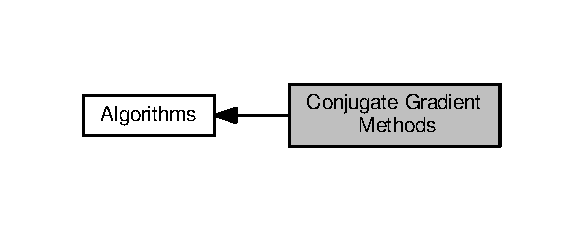
\includegraphics[width=280pt]{group__CGGroup}
\end{center}
\end{figure}
\subsection*{Namespaces}
\begin{DoxyCompactItemize}
\item 
 \hyperlink{namespaceSpacy_1_1CG}{Spacy\+::\+C\+G}
\begin{DoxyCompactList}\small\item\em Conjugate gradient methods for convex and nonconvex problems (C\+G, Truncated C\+G, Regularized C\+G and Truncated Regularized C\+G). \end{DoxyCompactList}\end{DoxyCompactItemize}
\subsection*{Classes}
\begin{DoxyCompactItemize}
\item 
class \hyperlink{classSpacy_1_1CG_1_1Solver}{Spacy\+::\+C\+G\+::\+Solver}
\begin{DoxyCompactList}\small\item\em Conjugate gradient method. \end{DoxyCompactList}\item 
class \hyperlink{classSpacy_1_1CG_1_1LinearSolver}{Spacy\+::\+C\+G\+::\+Linear\+Solver}
\begin{DoxyCompactList}\small\item\em Conjugate gradient solver satisfying the \hyperlink{group__ConceptGroup_ga582dd34334cdecc7b27883f4e8239490_IndefiniteLinearSolverConceptAnchor}{Indefinite\+Linear\+Solver\+Concept}. \end{DoxyCompactList}\item 
class \hyperlink{classSpacy_1_1CG_1_1Termination_1_1StrakosTichyEnergyError}{Spacy\+::\+C\+G\+::\+Termination\+::\+Strakos\+Tichy\+Energy\+Error}
\begin{DoxyCompactList}\small\item\em \hyperlink{namespaceSpacy_1_1CG_1_1Termination}{Termination} criterion for conjugate gradient methods based on an estimate of the relative energy error. \end{DoxyCompactList}\end{DoxyCompactItemize}
\subsection*{Typedefs}
\begin{DoxyCompactItemize}
\item 
using \hyperlink{group__CGGroup_gaa927be31b313bb4ce635668c77b55860_gaa927be31b313bb4ce635668c77b55860}{Spacy\+::\+C\+G\+::\+Termination\+Criterion} = boost\+::type\+\_\+erasure\+::any$<$ Concepts\+::\+C\+G\+::\+Termination\+Criterion\+Concept $>$
\begin{DoxyCompactList}\small\item\em \hyperlink{namespaceSpacy_1_1CG_1_1Termination}{Termination} criteria for conjugate gradient methods. \end{DoxyCompactList}\end{DoxyCompactItemize}
\subsection*{Functions}
\begin{DoxyCompactItemize}
\item 
C\+G\+::\+Linear\+Solver \hyperlink{group__CGGroup_gaafd9bf87164dd48991d2016aec8bad08_gaafd9bf87164dd48991d2016aec8bad08}{Spacy\+::make\+C\+G\+Solver} (Operator A, Callable\+Operator P, double relative\+Accuracy=1e-\/15, double eps=1e-\/15, bool verbose=false)
\begin{DoxyCompactList}\small\item\em Construct conjugate gradient method. \end{DoxyCompactList}\item 
C\+G\+::\+Linear\+Solver \hyperlink{group__CGGroup_gaf9ddae62858412fe5309d11aac7b8ed3_gaf9ddae62858412fe5309d11aac7b8ed3}{Spacy\+::make\+R\+C\+G\+Solver} (Operator A, Callable\+Operator P, double relative\+Accuracy=1e-\/15, double eps=1e-\/15, bool verbose=false)
\begin{DoxyCompactList}\small\item\em Construct regularized conjugate gradient method. \end{DoxyCompactList}\item 
C\+G\+::\+Linear\+Solver \hyperlink{group__CGGroup_ga5693f62a60708a49f51cf451991b96ec_ga5693f62a60708a49f51cf451991b96ec}{Spacy\+::make\+T\+C\+G\+Solver} (Operator A, Callable\+Operator P, double relative\+Accuracy=1e-\/15, double eps=1e-\/15, bool verbose=false)
\begin{DoxyCompactList}\small\item\em Construct truncated conjugate gradient method. \end{DoxyCompactList}\item 
C\+G\+::\+Linear\+Solver \hyperlink{group__CGGroup_ga66f5afbc97e887274b28be9c94aa3103_ga66f5afbc97e887274b28be9c94aa3103}{Spacy\+::make\+T\+R\+C\+G\+Solver} (Operator A, Callable\+Operator P, double relative\+Accuracy=1e-\/15, double eps=1e-\/15, bool verbose=false)
\begin{DoxyCompactList}\small\item\em Construct truncated regularized conjugate gradient method. \end{DoxyCompactList}\end{DoxyCompactItemize}


\subsection{Detailed Description}
Conjugate gradient methods for convex and nonconvex problems (C\+G, Truncated C\+G, Regularized C\+G and Truncated Regularized C\+G). 



\subsection{Typedef Documentation}
\hypertarget{group__CGGroup_gaa927be31b313bb4ce635668c77b55860_gaa927be31b313bb4ce635668c77b55860}{}\index{Conjugate Gradient Methods@{Conjugate Gradient Methods}!Termination\+Criterion@{Termination\+Criterion}}
\index{Termination\+Criterion@{Termination\+Criterion}!Conjugate Gradient Methods@{Conjugate Gradient Methods}}
\subsubsection[{Termination\+Criterion}]{\setlength{\rightskip}{0pt plus 5cm}using {\bf Spacy\+::\+C\+G\+::\+Termination\+Criterion} = typedef boost\+::type\+\_\+erasure\+::any$<$ Concepts\+::\+C\+G\+::\+Termination\+Criterion\+Concept $>$}\label{group__CGGroup_gaa927be31b313bb4ce635668c77b55860_gaa927be31b313bb4ce635668c77b55860}


\hyperlink{namespaceSpacy_1_1CG_1_1Termination}{Termination} criteria for conjugate gradient methods. 

\label{group__CGGroup_gaa927be31b313bb4ce635668c77b55860_CG_TerminationCriterionAnchor}%
\hypertarget{group__CGGroup_gaa927be31b313bb4ce635668c77b55860_CG_TerminationCriterionAnchor}{}%
See \hyperlink{group__CGConceptGroup_ga6b30d103c365816efcfb038d922aef07_CG_TerminationCriterionConceptAnchor}{Termination\+Criterion\+Concept}. 

\subsection{Function Documentation}
\hypertarget{group__CGGroup_gaafd9bf87164dd48991d2016aec8bad08_gaafd9bf87164dd48991d2016aec8bad08}{}\index{Conjugate Gradient Methods@{Conjugate Gradient Methods}!make\+C\+G\+Solver@{make\+C\+G\+Solver}}
\index{make\+C\+G\+Solver@{make\+C\+G\+Solver}!Conjugate Gradient Methods@{Conjugate Gradient Methods}}
\subsubsection[{make\+C\+G\+Solver}]{\setlength{\rightskip}{0pt plus 5cm}C\+G\+::\+Linear\+Solver Spacy\+::make\+C\+G\+Solver (
\begin{DoxyParamCaption}
\item[{{\bf Operator}}]{A, }
\item[{{\bf Callable\+Operator}}]{P, }
\item[{double}]{relative\+Accuracy = {\ttfamily 1e-\/15}, }
\item[{double}]{eps = {\ttfamily 1e-\/15}, }
\item[{bool}]{verbose = {\ttfamily false}}
\end{DoxyParamCaption}
)}\label{group__CGGroup_gaafd9bf87164dd48991d2016aec8bad08_gaafd9bf87164dd48991d2016aec8bad08}


Construct conjugate gradient method. 


\begin{DoxyParams}{Parameters}
{\em A} & operator \\
\hline
{\em P} & preconditioner \\
\hline
{\em relative\+Accuracy} & relative accuracy \\
\hline
{\em eps} & maximal attainable accuracy \\
\hline
{\em verbose} & verbosity \\
\hline
\end{DoxyParams}
\begin{DoxyReturn}{Returns}
C\+G\+Solver(A,P,\char`\"{}\+C\+G\char`\"{}) 
\end{DoxyReturn}
\hypertarget{group__CGGroup_gaf9ddae62858412fe5309d11aac7b8ed3_gaf9ddae62858412fe5309d11aac7b8ed3}{}\index{Conjugate Gradient Methods@{Conjugate Gradient Methods}!make\+R\+C\+G\+Solver@{make\+R\+C\+G\+Solver}}
\index{make\+R\+C\+G\+Solver@{make\+R\+C\+G\+Solver}!Conjugate Gradient Methods@{Conjugate Gradient Methods}}
\subsubsection[{make\+R\+C\+G\+Solver}]{\setlength{\rightskip}{0pt plus 5cm}C\+G\+::\+Linear\+Solver Spacy\+::make\+R\+C\+G\+Solver (
\begin{DoxyParamCaption}
\item[{{\bf Operator}}]{A, }
\item[{{\bf Callable\+Operator}}]{P, }
\item[{double}]{relative\+Accuracy = {\ttfamily 1e-\/15}, }
\item[{double}]{eps = {\ttfamily 1e-\/15}, }
\item[{bool}]{verbose = {\ttfamily false}}
\end{DoxyParamCaption}
)}\label{group__CGGroup_gaf9ddae62858412fe5309d11aac7b8ed3_gaf9ddae62858412fe5309d11aac7b8ed3}


Construct regularized conjugate gradient method. 


\begin{DoxyParams}{Parameters}
{\em A} & operator \\
\hline
{\em P} & preconditioner \\
\hline
{\em relative\+Accuracy} & relative accuracy \\
\hline
{\em eps} & maximal attainable accuracy \\
\hline
{\em verbose} & verbosity \\
\hline
\end{DoxyParams}
\begin{DoxyReturn}{Returns}
C\+G\+Solver(A,P,\char`\"{}\+R\+C\+G\char`\"{}) 
\end{DoxyReturn}
\hypertarget{group__CGGroup_ga5693f62a60708a49f51cf451991b96ec_ga5693f62a60708a49f51cf451991b96ec}{}\index{Conjugate Gradient Methods@{Conjugate Gradient Methods}!make\+T\+C\+G\+Solver@{make\+T\+C\+G\+Solver}}
\index{make\+T\+C\+G\+Solver@{make\+T\+C\+G\+Solver}!Conjugate Gradient Methods@{Conjugate Gradient Methods}}
\subsubsection[{make\+T\+C\+G\+Solver}]{\setlength{\rightskip}{0pt plus 5cm}C\+G\+::\+Linear\+Solver Spacy\+::make\+T\+C\+G\+Solver (
\begin{DoxyParamCaption}
\item[{{\bf Operator}}]{A, }
\item[{{\bf Callable\+Operator}}]{P, }
\item[{double}]{relative\+Accuracy = {\ttfamily 1e-\/15}, }
\item[{double}]{eps = {\ttfamily 1e-\/15}, }
\item[{bool}]{verbose = {\ttfamily false}}
\end{DoxyParamCaption}
)}\label{group__CGGroup_ga5693f62a60708a49f51cf451991b96ec_ga5693f62a60708a49f51cf451991b96ec}


Construct truncated conjugate gradient method. 


\begin{DoxyParams}{Parameters}
{\em A} & operator \\
\hline
{\em P} & preconditioner \\
\hline
{\em relative\+Accuracy} & relative accuracy \\
\hline
{\em eps} & maximal attainable accuracy \\
\hline
{\em verbose} & verbosity \\
\hline
\end{DoxyParams}
\begin{DoxyReturn}{Returns}
C\+G\+Solver(A,P,\char`\"{}\+T\+C\+G\char`\"{}) 
\end{DoxyReturn}
\hypertarget{group__CGGroup_ga66f5afbc97e887274b28be9c94aa3103_ga66f5afbc97e887274b28be9c94aa3103}{}\index{Conjugate Gradient Methods@{Conjugate Gradient Methods}!make\+T\+R\+C\+G\+Solver@{make\+T\+R\+C\+G\+Solver}}
\index{make\+T\+R\+C\+G\+Solver@{make\+T\+R\+C\+G\+Solver}!Conjugate Gradient Methods@{Conjugate Gradient Methods}}
\subsubsection[{make\+T\+R\+C\+G\+Solver}]{\setlength{\rightskip}{0pt plus 5cm}C\+G\+::\+Linear\+Solver Spacy\+::make\+T\+R\+C\+G\+Solver (
\begin{DoxyParamCaption}
\item[{{\bf Operator}}]{A, }
\item[{{\bf Callable\+Operator}}]{P, }
\item[{double}]{relative\+Accuracy = {\ttfamily 1e-\/15}, }
\item[{double}]{eps = {\ttfamily 1e-\/15}, }
\item[{bool}]{verbose = {\ttfamily false}}
\end{DoxyParamCaption}
)}\label{group__CGGroup_ga66f5afbc97e887274b28be9c94aa3103_ga66f5afbc97e887274b28be9c94aa3103}


Construct truncated regularized conjugate gradient method. 


\begin{DoxyParams}{Parameters}
{\em A} & operator \\
\hline
{\em P} & preconditioner \\
\hline
{\em relative\+Accuracy} & relative accuracy \\
\hline
{\em eps} & maximal attainable accuracy \\
\hline
{\em verbose} & verbosity \\
\hline
\end{DoxyParams}
\begin{DoxyReturn}{Returns}
C\+G\+Solver(A,P,\char`\"{}\+T\+R\+C\+G\char`\"{}) 
\end{DoxyReturn}

\hypertarget{group__CSGroup}{}\section{Composite Step Methods}
\label{group__CSGroup}\index{Composite Step Methods@{Composite Step Methods}}


Contains the affine covariant composite step method of \cite{Lubkoll2015}, \cite{Lubkoll2015a}.  


Collaboration diagram for Composite Step Methods\+:\nopagebreak
\begin{figure}[H]
\begin{center}
\leavevmode
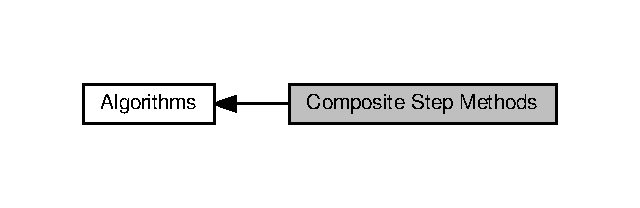
\includegraphics[width=307pt]{group__CSGroup}
\end{center}
\end{figure}
\subsection*{Classes}
\begin{DoxyCompactItemize}
\item 
class \hyperlink{classSpacy_1_1CompositeStep_1_1CubicModel}{Spacy\+::\+Composite\+Step\+::\+Cubic\+Model}
\begin{DoxyCompactList}\small\item\em The cubic regularized model for Affine\+Covariant\+Composite\+Steps. \end{DoxyCompactList}\end{DoxyCompactItemize}
\subsection*{Functions}
\begin{DoxyCompactItemize}
\item 
Functions\+\_\+1\+D\+::\+Quadratic \hyperlink{group__CSGroup_gad4acace8423370ac1b3d53a03fbde523_gad4acace8423370ac1b3d53a03fbde523}{Spacy\+::\+Composite\+Step\+::make\+Quadratic\+Model} (Real nu, const Vector \&dn, const Vector \&dt, const C2\+Functional \&L, const Vector \&x)
\begin{DoxyCompactList}\small\item\em Constructs the quadratic model of a Lagrange functional for a composite step method. \end{DoxyCompactList}\item 
Functions\+\_\+1\+D\+::\+Quadratic \hyperlink{group__CSGroup_ga2d9442c6e622766cb33dc14aa497c945_ga2d9442c6e622766cb33dc14aa497c945}{Spacy\+::\+Composite\+Step\+::make\+Quadratic\+Norm\+Model} (Real nu, const Vector \&dn, const Vector \&dt)
\begin{DoxyCompactList}\small\item\em Constructs the quadratic model a norm for a composite step method. \end{DoxyCompactList}\item 
Cubic\+Model \hyperlink{group__CSGroup_ga408c87c25b624012e03bca53e6ec3d10_ga408c87c25b624012e03bca53e6ec3d10}{Spacy\+::\+Composite\+Step\+::make\+Cubic\+Model} (Real nu, const Vector \&dn, const Vector \&dt, const C2\+Functional \&L, const Vector \&x, Real omega)
\begin{DoxyCompactList}\small\item\em Generate cubic regularized model for Affine\+Covariant\+Composite\+Steps. \end{DoxyCompactList}\item 
{\footnotesize template$<$class Model $>$ }\\Real \hyperlink{group__CSGroup_gadffb0e7fa07418c47de2474156d90a35_gadffb0e7fa07418c47de2474156d90a35}{Spacy\+::\+Composite\+Step\+::find\+Minimizer} (const Model \&f, Real a, Real b, Real eps=1e-\/2)
\begin{DoxyCompactList}\small\item\em Find global minimizer of $f$ in $[a,b]$. \end{DoxyCompactList}\end{DoxyCompactItemize}


\subsection{Detailed Description}
Contains the affine covariant composite step method of \cite{Lubkoll2015}, \cite{Lubkoll2015a}. 



\subsection{Function Documentation}
\hypertarget{group__CSGroup_gadffb0e7fa07418c47de2474156d90a35_gadffb0e7fa07418c47de2474156d90a35}{}\index{Composite Step Methods@{Composite Step Methods}!find\+Minimizer@{find\+Minimizer}}
\index{find\+Minimizer@{find\+Minimizer}!Composite Step Methods@{Composite Step Methods}}
\subsubsection[{find\+Minimizer}]{\setlength{\rightskip}{0pt plus 5cm}template$<$class Model $>$ Real Spacy\+::\+Composite\+Step\+::find\+Minimizer (
\begin{DoxyParamCaption}
\item[{const Model \&}]{f, }
\item[{{\bf Real}}]{a, }
\item[{{\bf Real}}]{b, }
\item[{{\bf Real}}]{eps = {\ttfamily 1e-\/2}}
\end{DoxyParamCaption}
)}\label{group__CSGroup_gadffb0e7fa07418c47de2474156d90a35_gadffb0e7fa07418c47de2474156d90a35}


Find global minimizer of $f$ in $[a,b]$. 


\begin{DoxyParams}{Parameters}
{\em f} & Nonlinear function $ f: \mathbb{R}\to\mathbb{R} $ \\
\hline
{\em a} & lower bound of the admissible interval \\
\hline
{\em b} & upper bound of the admissible interval \\
\hline
{\em eps} & relative accuracy \\
\hline
\end{DoxyParams}
\begin{DoxyReturn}{Returns}
$ x \in \mathrm{argmin}_{[a,b]} $ 
\end{DoxyReturn}
\hypertarget{group__CSGroup_ga408c87c25b624012e03bca53e6ec3d10_ga408c87c25b624012e03bca53e6ec3d10}{}\index{Composite Step Methods@{Composite Step Methods}!make\+Cubic\+Model@{make\+Cubic\+Model}}
\index{make\+Cubic\+Model@{make\+Cubic\+Model}!Composite Step Methods@{Composite Step Methods}}
\subsubsection[{make\+Cubic\+Model}]{\setlength{\rightskip}{0pt plus 5cm}Cubic\+Model Spacy\+::\+Composite\+Step\+::make\+Cubic\+Model (
\begin{DoxyParamCaption}
\item[{{\bf Real}}]{nu, }
\item[{const {\bf Vector} \&}]{dn, }
\item[{const {\bf Vector} \&}]{dt, }
\item[{const {\bf C2\+Functional} \&}]{L, }
\item[{const {\bf Vector} \&}]{x, }
\item[{{\bf Real}}]{omega}
\end{DoxyParamCaption}
)}\label{group__CSGroup_ga408c87c25b624012e03bca53e6ec3d10_ga408c87c25b624012e03bca53e6ec3d10}


Generate cubic regularized model for Affine\+Covariant\+Composite\+Steps. 


\begin{DoxyParams}{Parameters}
{\em nu} & normal step damping factor \\
\hline
{\em dn} & normal step \\
\hline
{\em dt} & tangential step \\
\hline
{\em L} & Lagrange functional \\
\hline
{\em x} & current iterate \\
\hline
{\em omega} & estimate of the Lipschitz constant of the second derivative of the Lagrangian \\
\hline
\end{DoxyParams}
\begin{DoxyReturn}{Returns}
\hyperlink{classSpacy_1_1CompositeStep_1_1CubicModel}{Cubic\+Model}( make\+Quadratic\+Model(nu,dn,dt,\+L,x), make\+Quadratic\+Norm\+Model(nu,dn,dt), omega ) 
\end{DoxyReturn}
\hypertarget{group__CSGroup_gad4acace8423370ac1b3d53a03fbde523_gad4acace8423370ac1b3d53a03fbde523}{}\index{Composite Step Methods@{Composite Step Methods}!make\+Quadratic\+Model@{make\+Quadratic\+Model}}
\index{make\+Quadratic\+Model@{make\+Quadratic\+Model}!Composite Step Methods@{Composite Step Methods}}
\subsubsection[{make\+Quadratic\+Model}]{\setlength{\rightskip}{0pt plus 5cm}Functions\+\_\+1\+D\+::\+Quadratic Spacy\+::\+Composite\+Step\+::make\+Quadratic\+Model (
\begin{DoxyParamCaption}
\item[{{\bf Real}}]{nu, }
\item[{const {\bf Vector} \&}]{dn, }
\item[{const {\bf Vector} \&}]{dt, }
\item[{const {\bf C2\+Functional} \&}]{L, }
\item[{const {\bf Vector} \&}]{x}
\end{DoxyParamCaption}
)}\label{group__CSGroup_gad4acace8423370ac1b3d53a03fbde523_gad4acace8423370ac1b3d53a03fbde523}


Constructs the quadratic model of a Lagrange functional for a composite step method. 


\begin{DoxyParams}{Parameters}
{\em nu} & normal step damping factor \\
\hline
{\em dn} & normal step \\
\hline
{\em dt} & tangential step \\
\hline
{\em L} & Lagrange functional \\
\hline
{\em x} & current iterate\\
\hline
\end{DoxyParams}
Constructs a quadratic function $ q(t)=a+bt+ct^2$, with
\begin{DoxyItemize}
\item $ a = L(x)+\nu L'(x)dn+\frac{\nu^2}{2}L''(x)(dn)^2 $
\item $ b = L'(x)dt + \nu L''(x)(dn,dt) $
\item $ c = \frac{1}{2}L''(x)(dt)^2 $
\end{DoxyItemize}

\begin{DoxyReturn}{Returns}
$ q(t)=a+bt+ct^2$ 
\end{DoxyReturn}
\hypertarget{group__CSGroup_ga2d9442c6e622766cb33dc14aa497c945_ga2d9442c6e622766cb33dc14aa497c945}{}\index{Composite Step Methods@{Composite Step Methods}!make\+Quadratic\+Norm\+Model@{make\+Quadratic\+Norm\+Model}}
\index{make\+Quadratic\+Norm\+Model@{make\+Quadratic\+Norm\+Model}!Composite Step Methods@{Composite Step Methods}}
\subsubsection[{make\+Quadratic\+Norm\+Model}]{\setlength{\rightskip}{0pt plus 5cm}Functions\+\_\+1\+D\+::\+Quadratic Spacy\+::\+Composite\+Step\+::make\+Quadratic\+Norm\+Model (
\begin{DoxyParamCaption}
\item[{{\bf Real}}]{nu, }
\item[{const {\bf Vector} \&}]{dn, }
\item[{const {\bf Vector} \&}]{dt}
\end{DoxyParamCaption}
)}\label{group__CSGroup_ga2d9442c6e622766cb33dc14aa497c945_ga2d9442c6e622766cb33dc14aa497c945}


Constructs the quadratic model a norm for a composite step method. 


\begin{DoxyParams}{Parameters}
{\em nu} & normal step damping factor \\
\hline
{\em dn} & normal step \\
\hline
{\em dt} & tangential step \\
\hline
\end{DoxyParams}
\begin{DoxyReturn}{Returns}
$ q(t)=\nu^2\|dn\|^2+2\nu(dn,dt)t+\|dt\|^2t^2 $ 
\end{DoxyReturn}

\hypertarget{group__ConceptGroup}{}\section{Concepts}
\label{group__ConceptGroup}\index{Concepts@{Concepts}}


Concepts for vectors, functional, operators, ...  


Collaboration diagram for Concepts\+:\nopagebreak
\begin{figure}[H]
\begin{center}
\leavevmode
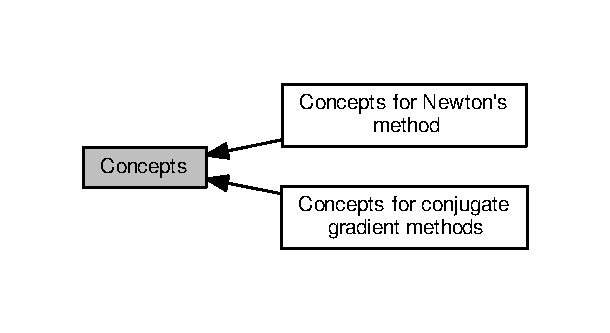
\includegraphics[width=293pt]{group__ConceptGroup}
\end{center}
\end{figure}
\subsection*{Modules}
\begin{DoxyCompactItemize}
\item 
\hyperlink{group__NewtonConceptGroup}{Concepts for Newton\textquotesingle{}s method}
\begin{DoxyCompactList}\small\item\em Concepts for damping strategy and termination criteria for Newton\textquotesingle{}s method. \end{DoxyCompactList}\item 
\hyperlink{group__CGConceptGroup}{Concepts for conjugate gradient methods}
\begin{DoxyCompactList}\small\item\em Concept for termination criteria for conjugate gradient methods. \end{DoxyCompactList}\end{DoxyCompactItemize}
\subsection*{Typedefs}
\begin{DoxyCompactItemize}
\item 
using \hyperlink{group__ConceptGroup_ga63426675cc05ccce03ead56a4fa90d96_ga63426675cc05ccce03ead56a4fa90d96}{Spacy\+::\+Concepts\+::\+Concept\+Base} = boost\+::mpl\+::vector$<$ boost\+::type\+\_\+erasure\+::copy\+\_\+constructible$<$$>$, boost\+::type\+\_\+erasure\+::typeid\+\_\+$<$$>$, boost\+::type\+\_\+erasure\+::relaxed $>$
\begin{DoxyCompactList}\small\item\em Base concept. \end{DoxyCompactList}\item 
using \hyperlink{group__ConceptGroup_ga30692db093ead5a1a074905363a2f043_ga30692db093ead5a1a074905363a2f043}{Spacy\+::\+Concepts\+::\+Dynamic\+Callable\+Operator\+Concept} = boost\+::mpl\+::vector$<$ Concept\+Base, boost\+::type\+\_\+erasure\+::callable$<$ Vector(double t, const Vector \&), const boost\+::type\+\_\+erasure\+::\+\_\+self $>$ $>$
\begin{DoxyCompactList}\small\item\em Concept defining the simplest possible time-\/dependent operator, only providing \hyperlink{classSpacy_1_1Vector}{Vector} operator()(double t, const Vector\&). \end{DoxyCompactList}\item 
using \hyperlink{group__ConceptGroup_ga2c979d268f0ca7a436776a9631d10af7_ga2c979d268f0ca7a436776a9631d10af7}{Spacy\+::\+Concepts\+::\+Dynamic\+Operator\+Concept} = boost\+::mpl\+::vector$<$ Dynamic\+Callable\+Operator\+Concept, has\+\_\+\+M$<$ boost\+::type\+\_\+erasure\+::any$<$ Linear\+Operator\+Concept $>$(), const boost\+::type\+\_\+erasure\+::\+\_\+self $>$, has\+\_\+domain$<$ const Vector\+Space \&(), const boost\+::type\+\_\+erasure\+::\+\_\+self $>$, has\+\_\+range$<$ const Vector\+Space \&(), const boost\+::type\+\_\+erasure\+::\+\_\+self $>$ $>$
\begin{DoxyCompactList}\small\item\em Concept defining general time-\/dependent operators. \end{DoxyCompactList}\item 
using \hyperlink{group__ConceptGroup_ga015b0d099011a2ef73a16aa9b36a7346_ga015b0d099011a2ef73a16aa9b36a7346}{Spacy\+::\+Concepts\+::\+Dynamic\+Linear\+Operator\+Concept} = boost\+::mpl\+::vector$<$ Dynamic\+Operator\+Concept, has\+\_\+solver$<$ const boost\+::type\+\_\+erasure\+::any$<$ Linear\+Solver\+Concept $>$ \&(), const boost\+::type\+\_\+erasure\+::\+\_\+self $>$ $>$
\begin{DoxyCompactList}\small\item\em Concept defining time-\/dependent linear operators. \end{DoxyCompactList}\item 
using \hyperlink{group__ConceptGroup_gaa7ef0ce2d66b0610035541b580564b11_gaa7ef0ce2d66b0610035541b580564b11}{Spacy\+::\+Concepts\+::\+Dynamic\+C1\+Operator\+Concept} = boost\+::mpl\+::vector$<$ Dynamic\+Operator\+Concept, has\+\_\+d1$<$ Vector(double t, const Vector \&, const Vector \&), const boost\+::type\+\_\+erasure\+::\+\_\+self $>$, has\+\_\+linearization$<$ boost\+::type\+\_\+erasure\+::any$<$ Linear\+Operator\+Concept $>$(double t, const Vector \&), const boost\+::type\+\_\+erasure\+::\+\_\+self $>$ $>$
\begin{DoxyCompactList}\small\item\em Concept defining time-\/dependent operators that are differentiable with respect to the spatial variable. \end{DoxyCompactList}\item 
using \hyperlink{group__ConceptGroup_ga6b5c97b0e58318ef98c43a9b8a7dae08_ga6b5c97b0e58318ef98c43a9b8a7dae08}{Spacy\+::\+Concepts\+::\+My\+Error\+Estimator\+Concept} = boost\+::mpl\+::vector$<$ Concept\+Base, boost\+::type\+\_\+erasure\+::callable$<$ double(const Vector \&, const Vector \&), const boost\+::type\+\_\+erasure\+::\+\_\+self $>$, has\+\_\+refine$<$ void()$>$ $>$
\begin{DoxyCompactList}\small\item\em Concept for time integrators. \end{DoxyCompactList}\item 
using \hyperlink{group__ConceptGroup_ga5273b50bd3e8c9a3f5a1e6b5f170836d_ga5273b50bd3e8c9a3f5a1e6b5f170836d}{Spacy\+::\+Concepts\+::\+Functional\+Concept} = boost\+::mpl\+::vector$<$ Concept\+Base, boost\+::type\+\_\+erasure\+::callable$<$ Real(const Vector \&), const boost\+::type\+\_\+erasure\+::\+\_\+self $>$, has\+\_\+domain$<$ const Vector\+Space \&(), const boost\+::type\+\_\+erasure\+::\+\_\+self $>$ $>$
\begin{DoxyCompactList}\small\item\em Concept for functionals. \end{DoxyCompactList}\item 
using \hyperlink{group__ConceptGroup_ga205b55d8291e0f2e143f116cf78bc54f_ga205b55d8291e0f2e143f116cf78bc54f}{Spacy\+::\+Concepts\+::\+C1\+Functional\+Concept} = boost\+::mpl\+::vector$<$ Functional\+Concept, has\+\_\+d1\+\_\+dual$<$ Vector(const Vector \&), const boost\+::type\+\_\+erasure\+::\+\_\+self $>$ $>$
\begin{DoxyCompactList}\small\item\em Concept for differentiable functionals. \end{DoxyCompactList}\item 
using \hyperlink{group__ConceptGroup_gafb4414561b07b27100cad81ecf152e47_gafb4414561b07b27100cad81ecf152e47}{Spacy\+::\+Concepts\+::\+C2\+Functional\+Concept} = boost\+::mpl\+::vector$<$ C1\+Functional\+Concept, has\+\_\+d2\+\_\+dual$<$ Vector(const Vector \&, const Vector \&), const boost\+::type\+\_\+erasure\+::\+\_\+self $>$, has\+\_\+hessian$<$ boost\+::type\+\_\+erasure\+::any$<$ Linear\+Operator\+Concept $>$(const Vector \&), const boost\+::type\+\_\+erasure\+::\+\_\+self $>$ $>$
\begin{DoxyCompactList}\small\item\em Concept for twice differentiable functionals. \end{DoxyCompactList}\item 
using \hyperlink{group__ConceptGroup_gac7d6a94c7131c8613e2ab26fddeb50bd_gac7d6a94c7131c8613e2ab26fddeb50bd}{Spacy\+::\+Concepts\+::\+Linear\+Solver\+Concept} = boost\+::mpl\+::vector$<$ Concept\+Base, boost\+::type\+\_\+erasure\+::callable$<$ Vector(const Vector \&), const boost\+::type\+\_\+erasure\+::\+\_\+self $>$ $>$
\begin{DoxyCompactList}\small\item\em Concept for linear solver implementations. Same as \hyperlink{group__ConceptGroup_gadec0c664abaacc2065dadd8b11cc8d30_CallableOperatorConceptAnchor}{Callable\+Operator\+Concept}. \end{DoxyCompactList}\item 
using \hyperlink{group__ConceptGroup_ga582dd34334cdecc7b27883f4e8239490_ga582dd34334cdecc7b27883f4e8239490}{Spacy\+::\+Concepts\+::\+Indefinite\+Linear\+Solver\+Concept} = boost\+::mpl\+::vector$<$ Linear\+Solver\+Concept, has\+\_\+is\+Positive\+Definite$<$ bool(), const boost\+::type\+\_\+erasure\+::\+\_\+self $>$ $>$
\begin{DoxyCompactList}\small\item\em Concept for linear solver implementations that monitor positive definiteness. \end{DoxyCompactList}\item 
using \hyperlink{group__ConceptGroup_ga8b6032c46f6e31840a2c956c6360549b_ga8b6032c46f6e31840a2c956c6360549b}{Spacy\+::\+Concepts\+::\+Norm\+Concept} = boost\+::mpl\+::vector$<$ Concept\+Base, boost\+::type\+\_\+erasure\+::callable$<$ Real(const Vector \&), const boost\+::type\+\_\+erasure\+::\+\_\+self $>$ $>$
\begin{DoxyCompactList}\small\item\em Concept for norm implementations. \end{DoxyCompactList}\item 
using \hyperlink{group__ConceptGroup_gadec0c664abaacc2065dadd8b11cc8d30_gadec0c664abaacc2065dadd8b11cc8d30}{Spacy\+::\+Concepts\+::\+Callable\+Operator\+Concept} = boost\+::mpl\+::vector$<$ Concept\+Base, boost\+::type\+\_\+erasure\+::callable$<$ Vector(const Vector \&), const boost\+::type\+\_\+erasure\+::\+\_\+self $>$ $>$
\begin{DoxyCompactList}\small\item\em Concept defining the simplest possible operator, only providing \hyperlink{classSpacy_1_1Vector}{Vector} operator()(const Vector\&). \end{DoxyCompactList}\item 
using \hyperlink{group__ConceptGroup_ga7d984281b647a6d8e4c0a7ea5faeb90e_ga7d984281b647a6d8e4c0a7ea5faeb90e}{Spacy\+::\+Concepts\+::\+Operator\+Concept} = boost\+::mpl\+::vector$<$ Callable\+Operator\+Concept, has\+\_\+domain$<$ const Vector\+Space \&(), const boost\+::type\+\_\+erasure\+::\+\_\+self $>$, has\+\_\+range$<$ const Vector\+Space \&(), const boost\+::type\+\_\+erasure\+::\+\_\+self $>$ $>$
\begin{DoxyCompactList}\small\item\em Concept defining general operators. \end{DoxyCompactList}\item 
using \hyperlink{group__ConceptGroup_gaf0e18e41c434cfceb77ccb8e785a8055_gaf0e18e41c434cfceb77ccb8e785a8055}{Spacy\+::\+Concepts\+::\+Linear\+Operator\+Concept} = boost\+::mpl\+::vector$<$ Operator\+Concept, Vector\+Concept, has\+\_\+solver$<$ boost\+::type\+\_\+erasure\+::any$<$ Linear\+Solver\+Concept $>$(), const boost\+::type\+\_\+erasure\+::\+\_\+self $>$ $>$
\begin{DoxyCompactList}\small\item\em Concept defining linear operators. \end{DoxyCompactList}\item 
using \hyperlink{group__ConceptGroup_ga14a12c741dc237e32862fa4bc315451b_ga14a12c741dc237e32862fa4bc315451b}{Spacy\+::\+Concepts\+::\+C1\+Operator\+Concept} = boost\+::mpl\+::vector$<$ Operator\+Concept, has\+\_\+d1$<$ Vector(const Vector \&, const Vector \&), const boost\+::type\+\_\+erasure\+::\+\_\+self $>$, has\+\_\+linearization$<$ boost\+::type\+\_\+erasure\+::any$<$ Linear\+Operator\+Concept $>$(const Vector \&), const boost\+::type\+\_\+erasure\+::\+\_\+self $>$ $>$
\begin{DoxyCompactList}\small\item\em Concept defining differentiable operators. \end{DoxyCompactList}\item 
using \hyperlink{group__ConceptGroup_ga1308724cda3078f228fb05c29556805d_ga1308724cda3078f228fb05c29556805d}{Spacy\+::\+Concepts\+::\+Scalar\+Product\+Concept} = boost\+::mpl\+::vector$<$ Concept\+Base, boost\+::type\+\_\+erasure\+::callable$<$ Real(const Vector \&, const Vector \&), const boost\+::type\+\_\+erasure\+::\+\_\+self $>$ $>$
\begin{DoxyCompactList}\small\item\em Concept for scalar products. \end{DoxyCompactList}\item 
using \hyperlink{group__ConceptGroup_ga45ecfe57ffb996aa97c9ff89a647f095_ga45ecfe57ffb996aa97c9ff89a647f095}{Spacy\+::\+Concepts\+::\+Time\+Integrator\+Concept} = boost\+::mpl\+::vector$<$ Concept\+Base, boost\+::type\+\_\+erasure\+::callable$<$ Vector(double, const Vector \&), const boost\+::type\+\_\+erasure\+::\+\_\+self $>$, has\+\_\+set\+Time\+Step$<$ void(double)$>$ $>$
\begin{DoxyCompactList}\small\item\em Concept for time integrators. \end{DoxyCompactList}\item 
using \hyperlink{group__ConceptGroup_gad6958389d1fa2758a8a64a0a24c36004_gad6958389d1fa2758a8a64a0a24c36004}{Spacy\+::\+Concepts\+::\+Vector\+Concept} = boost\+::mpl\+::vector$<$ Concept\+Base, boost\+::type\+\_\+erasure\+::assignable$<$$>$, boost\+::type\+\_\+erasure\+::multiply\+\_\+assignable$<$ boost\+::type\+\_\+erasure\+::\+\_\+self, double $>$, boost\+::type\+\_\+erasure\+::add\+\_\+assignable$<$$>$, boost\+::type\+\_\+erasure\+::subtract\+\_\+assignable$<$$>$, boost\+::type\+\_\+erasure\+::negatable$<$$>$, boost\+::type\+\_\+erasure\+::equality\+\_\+comparable$<$$>$, boost\+::type\+\_\+erasure\+::callable$<$ Vector(const boost\+::type\+\_\+erasure\+::\+\_\+self \&), const boost\+::type\+\_\+erasure\+::\+\_\+self $>$, has\+\_\+space$<$ const Vector\+Space $\ast$(), const boost\+::type\+\_\+erasure\+::\+\_\+self $>$, has\+\_\+to\+File$<$ void(const std\+::string \&), const boost\+::type\+\_\+erasure\+::\+\_\+self $>$ $>$
\begin{DoxyCompactList}\small\item\em Concept for vector implementations. \end{DoxyCompactList}\item 
using \hyperlink{group__ConceptGroup_ga3064301642b7c66b1b08f88a12a04645_ga3064301642b7c66b1b08f88a12a04645}{Spacy\+::\+Concepts\+::\+Vector\+Creator\+Concept} = boost\+::mpl\+::vector$<$ Concept\+Base, boost\+::type\+\_\+erasure\+::callable$<$ boost\+::type\+\_\+erasure\+::any$<$ Vector\+Concept $>$(const Vector\+Space $\ast$), const boost\+::type\+\_\+erasure\+::\+\_\+self $>$ $>$
\begin{DoxyCompactList}\small\item\em \hyperlink{classSpacy_1_1Vector}{Vector} creator concept. \end{DoxyCompactList}\end{DoxyCompactItemize}


\subsection{Detailed Description}
Concepts for vectors, functional, operators, ... 

The concepts are employed with Boost.\+Type\+Erasure, i.\+e. Vector\+Concept yields the type boost\+::type\+\_\+erasure\+::any$<$\+Vector\+Concept$>$. 

\subsection{Typedef Documentation}
\hypertarget{group__ConceptGroup_ga205b55d8291e0f2e143f116cf78bc54f_ga205b55d8291e0f2e143f116cf78bc54f}{}\index{Concepts@{Concepts}!C1\+Functional\+Concept@{C1\+Functional\+Concept}}
\index{C1\+Functional\+Concept@{C1\+Functional\+Concept}!Concepts@{Concepts}}
\subsubsection[{C1\+Functional\+Concept}]{\setlength{\rightskip}{0pt plus 5cm}using {\bf Spacy\+::\+Concepts\+::\+C1\+Functional\+Concept} = typedef boost\+::mpl\+::vector$<$ Functional\+Concept , has\+\_\+d1\+\_\+dual$<$Vector(const Vector\&), const boost\+::type\+\_\+erasure\+::\+\_\+self$>$ $>$}\label{group__ConceptGroup_ga205b55d8291e0f2e143f116cf78bc54f_ga205b55d8291e0f2e143f116cf78bc54f}


Concept for differentiable functionals. 

\label{group__ConceptGroup_ga205b55d8291e0f2e143f116cf78bc54f_C1FunctionalConceptAnchor}%
\hypertarget{group__ConceptGroup_ga205b55d8291e0f2e143f116cf78bc54f_C1FunctionalConceptAnchor}{}%
The minimal signature of a differentiable functional is 
\begin{DoxyCode}
1 // A differentiable functional f: X->R.
2 class MyC1Functional
3 \{
4 public:
5   // Copy constructor, possibly default-generated.
6   MyC1Functional(const MyC1Functional&);
7 
8   // Move constructor, possibly default-generated.
9   MyC1Functional(MyC1Functional&&);
10 
11   // Compute f(x).
12   double operator()(const ::Spacy::Vector& x) const;
13 
14   // Compute f'(x) as element of X*.
15   ::Spacy::Vector d1(const ::Spacy::Vector& x) const;
16 
17   // Access underlying domain.
18   const VectorSpace& domain() const;
19 \};
\end{DoxyCode}


See \hyperlink{group__SpacyGroup_gaa7cb8ef6c287b0af0352d3dd0eb9f200_C1FunctionalAnchor}{\+:\+:Spacy\+:\+:C1\+Functional}. \hypertarget{group__ConceptGroup_ga14a12c741dc237e32862fa4bc315451b_ga14a12c741dc237e32862fa4bc315451b}{}\index{Concepts@{Concepts}!C1\+Operator\+Concept@{C1\+Operator\+Concept}}
\index{C1\+Operator\+Concept@{C1\+Operator\+Concept}!Concepts@{Concepts}}
\subsubsection[{C1\+Operator\+Concept}]{\setlength{\rightskip}{0pt plus 5cm}using {\bf Spacy\+::\+Concepts\+::\+C1\+Operator\+Concept} = typedef boost\+::mpl\+::vector$<$ Operator\+Concept , has\+\_\+d1$<$Vector(const Vector\&,const Vector\&), const boost\+::type\+\_\+erasure\+::\+\_\+self$>$ , has\+\_\+linearization$<$boost\+::type\+\_\+erasure\+::any$<$Linear\+Operator\+Concept$>$(const Vector\&), const boost\+::type\+\_\+erasure\+::\+\_\+self$>$ $>$}\label{group__ConceptGroup_ga14a12c741dc237e32862fa4bc315451b_ga14a12c741dc237e32862fa4bc315451b}


Concept defining differentiable operators. 

\label{group__ConceptGroup_ga14a12c741dc237e32862fa4bc315451b_C1OperatorConceptAnchor}%
\hypertarget{group__ConceptGroup_ga14a12c741dc237e32862fa4bc315451b_C1OperatorConceptAnchor}{}%
The minimal signature for a differentiable operator is\+: 
\begin{DoxyCode}
1 // My differentiable operator A: X->Y.
2 class MyOperator
3 \{
4 public:
5   // Copy constructor.
6   MyOperator(const MyOperator&);
7 
8   // Move constructor.
9   MyOperator(MyOperator&&);
10 
11   // Compute A(x).
12   ::Spacy::Vector operator()(const ::Spacy::Vector& x) const;
13 
14   // Compute A'(x)dx.
15   ::Spacy::Vector d1(const ::Spacy::Vector& x, const ::Spacy::Vector& dx) const;
16 
17   // Get linearization representing A'(x).
18  ::Spacy::LinearOperator linearization(const ::Spacy::Vector& x) const;
19 
20   // Access domain space.
21   const VectorSpace& domain() const;
22 
23   // Access range space.
24   const VectorSpace& range() const;
25 \};
\end{DoxyCode}


See \hyperlink{group__SpacyGroup_ga87ae8cb0d7a567a4bb181e0a9f182620_C1OperatorAnchor}{\+:\+:Spacy\+:\+:C1\+Operator}. \hypertarget{group__ConceptGroup_gafb4414561b07b27100cad81ecf152e47_gafb4414561b07b27100cad81ecf152e47}{}\index{Concepts@{Concepts}!C2\+Functional\+Concept@{C2\+Functional\+Concept}}
\index{C2\+Functional\+Concept@{C2\+Functional\+Concept}!Concepts@{Concepts}}
\subsubsection[{C2\+Functional\+Concept}]{\setlength{\rightskip}{0pt plus 5cm}using {\bf Spacy\+::\+Concepts\+::\+C2\+Functional\+Concept} = typedef boost\+::mpl\+::vector$<$ C1\+Functional\+Concept , has\+\_\+d2\+\_\+dual$<$Vector(const Vector\&,const Vector\&), const boost\+::type\+\_\+erasure\+::\+\_\+self$>$ , has\+\_\+hessian$<$boost\+::type\+\_\+erasure\+::any$<$Linear\+Operator\+Concept$>$(const Vector\&), const boost\+::type\+\_\+erasure\+::\+\_\+self$>$ $>$}\label{group__ConceptGroup_gafb4414561b07b27100cad81ecf152e47_gafb4414561b07b27100cad81ecf152e47}


Concept for twice differentiable functionals. 

\label{group__ConceptGroup_gafb4414561b07b27100cad81ecf152e47_C2FunctionalConceptAnchor}%
\hypertarget{group__ConceptGroup_gafb4414561b07b27100cad81ecf152e47_C2FunctionalConceptAnchor}{}%
The minimal signature of a twice differentiable functional is 
\begin{DoxyCode}
1 // A twice differentiable functional f: X->R.
2 class MyC2Functional
3 \{
4 public:
5   // Copy constructor, possibly default-generated.
6   MyC2Functional(const MyC2Functional&);
7 
8   // Move constructor, possibly default-generated.
9   MyC2Functional(MyC2Functional&&);
10 
11   // Compute f(x).
12   double operator()(const ::Spacy::Vector& x) const;
13 
14   // Compute f'(x) as element of X*.
15   ::Spacy::Vector d1(const ::Spacy::Vector& x) const;
16 
17   // Compute f''(x)dx as element of X*.
18   ::Spacy::Vector d2(const ::Spacy::Vector& x, const ::Spacy::Vector& dx) const;
19 
20   // Access f''(x) as mapping f''(x): X->X*.
21   LinearOperator hessian(const ::Spacy::Vector& x);
22 
23   // Access underlying domain.
24   const VectorSpace& domain() const;
25 \};
\end{DoxyCode}


See \hyperlink{group__SpacyGroup_gaf5b89e117806134b06a1ce4629fb2b65_C2FunctionalAnchor}{\+:\+:Spacy\+:\+:C2\+Functional}. \hypertarget{group__ConceptGroup_gadec0c664abaacc2065dadd8b11cc8d30_gadec0c664abaacc2065dadd8b11cc8d30}{}\index{Concepts@{Concepts}!Callable\+Operator\+Concept@{Callable\+Operator\+Concept}}
\index{Callable\+Operator\+Concept@{Callable\+Operator\+Concept}!Concepts@{Concepts}}
\subsubsection[{Callable\+Operator\+Concept}]{\setlength{\rightskip}{0pt plus 5cm}using {\bf Spacy\+::\+Concepts\+::\+Callable\+Operator\+Concept} = typedef boost\+::mpl\+::vector$<$ Concept\+Base , boost\+::type\+\_\+erasure\+::callable$<$Vector(const Vector\&), const boost\+::type\+\_\+erasure\+::\+\_\+self$>$ $>$}\label{group__ConceptGroup_gadec0c664abaacc2065dadd8b11cc8d30_gadec0c664abaacc2065dadd8b11cc8d30}


Concept defining the simplest possible operator, only providing \hyperlink{classSpacy_1_1Vector}{Vector} operator()(const Vector\&). 

\label{group__ConceptGroup_gadec0c664abaacc2065dadd8b11cc8d30_CallableOperatorConceptAnchor}%
\hypertarget{group__ConceptGroup_gadec0c664abaacc2065dadd8b11cc8d30_CallableOperatorConceptAnchor}{}%
The minimal signature of a callable operator is\+: 
\begin{DoxyCode}
1 // My callable operator A: X->Y.
2 class MyOperator
3 \{
4 public:
5   // Copy constructor.
6   MyOperator(const MyOperator&);
7 
8   // Move constructor.
9   MyOperator(MyOperator&&);
10 
11   // Compute A(x).
12   ::Spacy::Vector operator()(const ::Spacy::Vector& x) const;
13 \};
\end{DoxyCode}


See \hyperlink{group__SpacyGroup_ga2b74020d806ad800795cdd97dab3466f_CallableOperatorAnchor}{\+:\+:Spacy\+:\+:Callable\+Operator}. \hypertarget{group__ConceptGroup_ga63426675cc05ccce03ead56a4fa90d96_ga63426675cc05ccce03ead56a4fa90d96}{}\index{Concepts@{Concepts}!Concept\+Base@{Concept\+Base}}
\index{Concept\+Base@{Concept\+Base}!Concepts@{Concepts}}
\subsubsection[{Concept\+Base}]{\setlength{\rightskip}{0pt plus 5cm}using {\bf Spacy\+::\+Concepts\+::\+Concept\+Base} = typedef boost\+::mpl\+::vector$<$ boost\+::type\+\_\+erasure\+::copy\+\_\+constructible$<$$>$ , boost\+::type\+\_\+erasure\+::typeid\+\_\+$<$$>$ , boost\+::type\+\_\+erasure\+::relaxed $>$}\label{group__ConceptGroup_ga63426675cc05ccce03ead56a4fa90d96_ga63426675cc05ccce03ead56a4fa90d96}


Base concept. 

Requires copy-\/constructability, provides run-\/time type information and some convenience functions with boost\+::type\+\_\+erasure\+::relaxed. \hypertarget{group__ConceptGroup_gaa7ef0ce2d66b0610035541b580564b11_gaa7ef0ce2d66b0610035541b580564b11}{}\index{Concepts@{Concepts}!Dynamic\+C1\+Operator\+Concept@{Dynamic\+C1\+Operator\+Concept}}
\index{Dynamic\+C1\+Operator\+Concept@{Dynamic\+C1\+Operator\+Concept}!Concepts@{Concepts}}
\subsubsection[{Dynamic\+C1\+Operator\+Concept}]{\setlength{\rightskip}{0pt plus 5cm}using {\bf Spacy\+::\+Concepts\+::\+Dynamic\+C1\+Operator\+Concept} = typedef boost\+::mpl\+::vector$<$ Dynamic\+Operator\+Concept , has\+\_\+d1$<$Vector(double t, const Vector\&,const Vector\&), const boost\+::type\+\_\+erasure\+::\+\_\+self$>$ , has\+\_\+linearization$<$boost\+::type\+\_\+erasure\+::any$<$Linear\+Operator\+Concept$>$(double t, const Vector\&), const boost\+::type\+\_\+erasure\+::\+\_\+self$>$ $>$}\label{group__ConceptGroup_gaa7ef0ce2d66b0610035541b580564b11_gaa7ef0ce2d66b0610035541b580564b11}


Concept defining time-\/dependent operators that are differentiable with respect to the spatial variable. 

\label{group__ConceptGroup_gaa7ef0ce2d66b0610035541b580564b11_DynamicC1OperatorConceptAnchor}%
\hypertarget{group__ConceptGroup_gaa7ef0ce2d66b0610035541b580564b11_DynamicC1OperatorConceptAnchor}{}%
The minimal signature for a time-\/dependent differentiable operator is\+: 
\begin{DoxyCode}
1 // My differentiable operator A: [0,T[ \(\backslash\)times X -> Y.
2 class MyOperator
3 \{
4 public:
5   // Copy constructor.
6   MyOperator(const MyOperator&);
7 
8   // Move constructor.
9   MyOperator(MyOperator&&);
10 
11   // Compute A(t,x).
12   ::Spacy::Vector operator()(double t, const ::Spacy::Vector& x) const;
13 
14   // Compute A\_x(t,x)dx.
15   ::Spacy::Vector d1(double t, const ::Spacy::Vector& x, const ::Spacy::Vector& dx) const;
16 
17   // Get linearization representing A\_x(t,x).
18  ::Spacy::LinearOperator linearization(double t, const ::Spacy::Vector& x) const;
19 
20   // Access mass matrix.
21   LinearOperator M() const;
22 
23   // Access domain space.
24   const VectorSpace& domain() const;
25 
26   // Access range space.
27   const VectorSpace& range() const;
28 \};
\end{DoxyCode}


See \hyperlink{group__SpacyGroup_gabc9c830d2a7e020bcab097b10ee6f642_DynamicC1OperatorAnchor}{\+:\+:Spacy\+:\+:Dynamic\+C1\+Operator}. \hypertarget{group__ConceptGroup_ga30692db093ead5a1a074905363a2f043_ga30692db093ead5a1a074905363a2f043}{}\index{Concepts@{Concepts}!Dynamic\+Callable\+Operator\+Concept@{Dynamic\+Callable\+Operator\+Concept}}
\index{Dynamic\+Callable\+Operator\+Concept@{Dynamic\+Callable\+Operator\+Concept}!Concepts@{Concepts}}
\subsubsection[{Dynamic\+Callable\+Operator\+Concept}]{\setlength{\rightskip}{0pt plus 5cm}using {\bf Spacy\+::\+Concepts\+::\+Dynamic\+Callable\+Operator\+Concept} = typedef boost\+::mpl\+::vector$<$ Concept\+Base , boost\+::type\+\_\+erasure\+::callable$<$Vector(double t, const Vector\&), const boost\+::type\+\_\+erasure\+::\+\_\+self$>$ $>$}\label{group__ConceptGroup_ga30692db093ead5a1a074905363a2f043_ga30692db093ead5a1a074905363a2f043}


Concept defining the simplest possible time-\/dependent operator, only providing \hyperlink{classSpacy_1_1Vector}{Vector} operator()(double t, const Vector\&). 

\label{group__ConceptGroup_ga30692db093ead5a1a074905363a2f043_DynamicCallableOperatorConceptAnchor}%
\hypertarget{group__ConceptGroup_ga30692db093ead5a1a074905363a2f043_DynamicCallableOperatorConceptAnchor}{}%
The minimal signature of a time-\/dependent callable operator is\+: 
\begin{DoxyCode}
1 // My callable operator A: [0,T[ \(\backslash\)times X -> Y.
2 class MyOperator
3 \{
4 public:
5   // Copy constructor.
6   MyOperator(const MyOperator&);
7 
8   // Move constructor.
9   MyOperator(MyOperator&&);
10 
11   // Compute A(t,x).
12   ::Spacy::Vector operator()(double t, const ::Spacy::Vector& x) const;
13 \};
\end{DoxyCode}


See \hyperlink{group__SpacyGroup_ga750d55072f7a3a16a1263961147333c0_DynamicCallableOperatorAnchor}{\+:\+:Spacy\+:\+:Dynamic\+Callable\+Operator}. \hypertarget{group__ConceptGroup_ga015b0d099011a2ef73a16aa9b36a7346_ga015b0d099011a2ef73a16aa9b36a7346}{}\index{Concepts@{Concepts}!Dynamic\+Linear\+Operator\+Concept@{Dynamic\+Linear\+Operator\+Concept}}
\index{Dynamic\+Linear\+Operator\+Concept@{Dynamic\+Linear\+Operator\+Concept}!Concepts@{Concepts}}
\subsubsection[{Dynamic\+Linear\+Operator\+Concept}]{\setlength{\rightskip}{0pt plus 5cm}using {\bf Spacy\+::\+Concepts\+::\+Dynamic\+Linear\+Operator\+Concept} = typedef boost\+::mpl\+::vector$<$ Dynamic\+Operator\+Concept , has\+\_\+solver$<$const boost\+::type\+\_\+erasure\+::any$<$Linear\+Solver\+Concept$>$\&(), const boost\+::type\+\_\+erasure\+::\+\_\+self$>$ $>$}\label{group__ConceptGroup_ga015b0d099011a2ef73a16aa9b36a7346_ga015b0d099011a2ef73a16aa9b36a7346}


Concept defining time-\/dependent linear operators. 

\label{group__ConceptGroup_ga015b0d099011a2ef73a16aa9b36a7346_DynamicLinearOperatorConceptAnchor}%
\hypertarget{group__ConceptGroup_ga015b0d099011a2ef73a16aa9b36a7346_DynamicLinearOperatorConceptAnchor}{}%
The minimal signature of a time-\/dependent linear operator is\+: 
\begin{DoxyCode}
1 // My linear operator A: [0,T[ \(\backslash\)times X -> Y.
2 class MyLinearOperator
3 \{
4 public:
5   // Copy constructor.
6   MyLinearOperator(const MyLinearOperator&);
7 
8   // Move constructor.
9   MyLinearOperator(MyLinearOperator&&);
10 
11   // Compute A(t,x).
12   ::Spacy::Vector operator()(double t, const ::Spacy::Vector& x) const;
13 
14   // Access solver for the computation of A(t)^-1.
15   ::Spacy::LinearSolver solver() const;
16 
17   // Access domain space.
18   const VectorSpace& domain() const;
19 
20   // Access range space.
21   const VectorSpace& range() const;
22 \};
\end{DoxyCode}


See \hyperlink{group__SpacyGroup_gaad10aa7d5443703377b768fa41a3c7ea_DynamicLinearOperatorAnchor}{\+:\+:Spacy\+:\+:Dynamic\+Linear\+Operator}. \hypertarget{group__ConceptGroup_ga2c979d268f0ca7a436776a9631d10af7_ga2c979d268f0ca7a436776a9631d10af7}{}\index{Concepts@{Concepts}!Dynamic\+Operator\+Concept@{Dynamic\+Operator\+Concept}}
\index{Dynamic\+Operator\+Concept@{Dynamic\+Operator\+Concept}!Concepts@{Concepts}}
\subsubsection[{Dynamic\+Operator\+Concept}]{\setlength{\rightskip}{0pt plus 5cm}using {\bf Spacy\+::\+Concepts\+::\+Dynamic\+Operator\+Concept} = typedef boost\+::mpl\+::vector$<$ Dynamic\+Callable\+Operator\+Concept , has\+\_\+\+M$<$boost\+::type\+\_\+erasure\+::any$<$ Linear\+Operator\+Concept $>$(), const boost\+::type\+\_\+erasure\+::\+\_\+self$>$ , has\+\_\+domain$<$const Vector\+Space\&(), const boost\+::type\+\_\+erasure\+::\+\_\+self$>$ , has\+\_\+range$<$const Vector\+Space\&(), const boost\+::type\+\_\+erasure\+::\+\_\+self$>$ $>$}\label{group__ConceptGroup_ga2c979d268f0ca7a436776a9631d10af7_ga2c979d268f0ca7a436776a9631d10af7}


Concept defining general time-\/dependent operators. 

\label{group__ConceptGroup_ga2c979d268f0ca7a436776a9631d10af7_DynamicOperatorConceptAnchor}%
\hypertarget{group__ConceptGroup_ga2c979d268f0ca7a436776a9631d10af7_DynamicOperatorConceptAnchor}{}%
The minimal signature of a time-\/dependent operator is\+: 
\begin{DoxyCode}
1 // My operator A: [0,T[ \(\backslash\)times X -> Y.
2 class MyOperator
3 \{
4 public:
5   // Copy constructor.
6   MyOperator(const MyOperator&);
7 
8   // Move constructor.
9   MyOperator(MyOperator&&);
10 
11   // Compute A(t,x).
12   ::Spacy::Vector operator()(double t, const ::Spacy::Vector& x) const;
13 
14   // Access domain space.
15   const VectorSpace& domain() const;
16 
17   // Access mass matrix.
18   LinearOperator M() const;
19 
20   // Access range space.
21   const VectorSpace& range() const;
22 \};
\end{DoxyCode}


See \+:\+:Spacy\+:\+:Dynamic\+Operator. \hypertarget{group__ConceptGroup_ga5273b50bd3e8c9a3f5a1e6b5f170836d_ga5273b50bd3e8c9a3f5a1e6b5f170836d}{}\index{Concepts@{Concepts}!Functional\+Concept@{Functional\+Concept}}
\index{Functional\+Concept@{Functional\+Concept}!Concepts@{Concepts}}
\subsubsection[{Functional\+Concept}]{\setlength{\rightskip}{0pt plus 5cm}using {\bf Spacy\+::\+Concepts\+::\+Functional\+Concept} = typedef boost\+::mpl\+::vector$<$ Concept\+Base, boost\+::type\+\_\+erasure\+::callable$<$Real(const Vector\&), const boost\+::type\+\_\+erasure\+::\+\_\+self$>$, has\+\_\+domain$<$const Vector\+Space\&(), const boost\+::type\+\_\+erasure\+::\+\_\+self$>$ $>$}\label{group__ConceptGroup_ga5273b50bd3e8c9a3f5a1e6b5f170836d_ga5273b50bd3e8c9a3f5a1e6b5f170836d}


Concept for functionals. 

\label{group__ConceptGroup_ga5273b50bd3e8c9a3f5a1e6b5f170836d_FunctionalConceptAnchor}%
\hypertarget{group__ConceptGroup_ga5273b50bd3e8c9a3f5a1e6b5f170836d_FunctionalConceptAnchor}{}%
The minimal signature of a functional is\+: 
\begin{DoxyCode}
1 // A functional f: X->R.
2 class MyFunctional
3 \{
4 public:
5   // Compute f(x).
6   double operator()(const ::Spacy::Vector& x) const;
7 
8   // Access underlying domain.
9   const VectorSpace& domain() const;
10 \};
\end{DoxyCode}


See \hyperlink{group__SpacyGroup_ga673218f603c93790864aef12c89d3a35_FunctionalAnchor}{\+:\+:Spacy\+:\+:Functional}. \hypertarget{group__ConceptGroup_ga582dd34334cdecc7b27883f4e8239490_ga582dd34334cdecc7b27883f4e8239490}{}\index{Concepts@{Concepts}!Indefinite\+Linear\+Solver\+Concept@{Indefinite\+Linear\+Solver\+Concept}}
\index{Indefinite\+Linear\+Solver\+Concept@{Indefinite\+Linear\+Solver\+Concept}!Concepts@{Concepts}}
\subsubsection[{Indefinite\+Linear\+Solver\+Concept}]{\setlength{\rightskip}{0pt plus 5cm}using {\bf Spacy\+::\+Concepts\+::\+Indefinite\+Linear\+Solver\+Concept} = typedef boost\+::mpl\+::vector$<$ Linear\+Solver\+Concept , has\+\_\+is\+Positive\+Definite$<$bool(), const boost\+::type\+\_\+erasure\+::\+\_\+self$>$ $>$}\label{group__ConceptGroup_ga582dd34334cdecc7b27883f4e8239490_ga582dd34334cdecc7b27883f4e8239490}


Concept for linear solver implementations that monitor positive definiteness. 

\label{group__ConceptGroup_ga582dd34334cdecc7b27883f4e8239490_IndefiniteLinearSolverConceptAnchor}%
\hypertarget{group__ConceptGroup_ga582dd34334cdecc7b27883f4e8239490_IndefiniteLinearSolverConceptAnchor}{}%
The minimal signature of a general linear solver is\+: 
\begin{DoxyCode}
1 // My general linear solver S representing A^-1.
2 class MyIndefiniteLinearSolver
3 \{
4 public:
5   // Copy constructor.
6   MyIndefiniteLinearSolver(const MyIndefiniteLinearSolver&);
7 
8   // Move constructor.
9   MyIndefiniteLinearSolver(MyIndefiniteLinearSolver&&);
10 
11   // Compute A^-1(x).
12   ::Spacy::Vector operator()(const ::Spacy::Vector& x) const;
13 
14   // Check if A is positive definite
15   bool isPositiveDefinite() const;
16 \};
\end{DoxyCode}


See \hyperlink{namespaceSpacy_a168383be933a8316169c145f5e419604_IndefiniteLinearSolverAnchor}{\+:\+:Spacy\+:\+:Indefinite\+Linear\+Solver}. \hypertarget{group__ConceptGroup_gaf0e18e41c434cfceb77ccb8e785a8055_gaf0e18e41c434cfceb77ccb8e785a8055}{}\index{Concepts@{Concepts}!Linear\+Operator\+Concept@{Linear\+Operator\+Concept}}
\index{Linear\+Operator\+Concept@{Linear\+Operator\+Concept}!Concepts@{Concepts}}
\subsubsection[{Linear\+Operator\+Concept}]{\setlength{\rightskip}{0pt plus 5cm}using {\bf Spacy\+::\+Concepts\+::\+Linear\+Operator\+Concept} = typedef boost\+::mpl\+::vector$<$ Operator\+Concept , Vector\+Concept , has\+\_\+solver$<$boost\+::type\+\_\+erasure\+::any$<$Linear\+Solver\+Concept$>$(), const boost\+::type\+\_\+erasure\+::\+\_\+self$>$ $>$}\label{group__ConceptGroup_gaf0e18e41c434cfceb77ccb8e785a8055_gaf0e18e41c434cfceb77ccb8e785a8055}


Concept defining linear operators. 

\label{group__ConceptGroup_gaf0e18e41c434cfceb77ccb8e785a8055_LinearOperatorConceptAnchor}%
\hypertarget{group__ConceptGroup_gaf0e18e41c434cfceb77ccb8e785a8055_LinearOperatorConceptAnchor}{}%
The minimal signature of a linear operator is\+: 
\begin{DoxyCode}
1 // My linear operator A: X->Y.
2 class MyLinearOperator
3 \{
4 public:
5   // Copy constructor.
6   MyLinearOperator(const MyLinearOperator&);
7 
8   // Move constructor.
9   MyLinearOperator(MyLinearOperator&&);
10 
11   // Compute A(x).
12   ::Spacy::Vector operator()(const ::Spacy::Vector& x) const;
13 
14   // Access solver for the computation of A^-1.
15   ::Spacy::LinearSolver solver() const;
16 
17   // Access domain space.
18   const VectorSpace& domain() const;
19 
20   // Access range space.
21   const VectorSpace& range() const;
22 \};
\end{DoxyCode}


See \hyperlink{group__SpacyGroup_ga584f7b9d82a844302ba0d77c3a1b6640_LinearOperatorAnchor}{\+:\+:Spacy\+:\+:Linear\+Operator}. \hypertarget{group__ConceptGroup_gac7d6a94c7131c8613e2ab26fddeb50bd_gac7d6a94c7131c8613e2ab26fddeb50bd}{}\index{Concepts@{Concepts}!Linear\+Solver\+Concept@{Linear\+Solver\+Concept}}
\index{Linear\+Solver\+Concept@{Linear\+Solver\+Concept}!Concepts@{Concepts}}
\subsubsection[{Linear\+Solver\+Concept}]{\setlength{\rightskip}{0pt plus 5cm}using {\bf Spacy\+::\+Concepts\+::\+Linear\+Solver\+Concept} = typedef boost\+::mpl\+::vector$<$ Concept\+Base , boost\+::type\+\_\+erasure\+::callable$<$Vector(const Vector\&), const boost\+::type\+\_\+erasure\+::\+\_\+self$>$ $>$}\label{group__ConceptGroup_gac7d6a94c7131c8613e2ab26fddeb50bd_gac7d6a94c7131c8613e2ab26fddeb50bd}


Concept for linear solver implementations. Same as \hyperlink{group__ConceptGroup_gadec0c664abaacc2065dadd8b11cc8d30_CallableOperatorConceptAnchor}{Callable\+Operator\+Concept}. 

\label{group__ConceptGroup_gac7d6a94c7131c8613e2ab26fddeb50bd_LinearSolverConceptAnchor}%
\hypertarget{group__ConceptGroup_gac7d6a94c7131c8613e2ab26fddeb50bd_LinearSolverConceptAnchor}{}%
The minimal signature of a linear solver is\+: 
\begin{DoxyCode}
1 // My linear solver representing A^-1.
2 class MyLinearSolver
3 \{
4 public:
5   // Copy constructor.
6   MyLinearSolver(const MyLinearSolver&);
7 
8   // Move constructor.
9   MyLinearSolver(MyLinearSolver&&);
10 
11   // Compute A^-1(x).
12   ::Spacy::Vector operator()(const ::Spacy::Vector& x) const;
13 \};
\end{DoxyCode}


See \hyperlink{namespaceSpacy_a7d5cd1c6fb9dd85aa345b536caf30bba_LinearSolverAnchor}{\+:\+:Spacy\+:\+:Linear\+Solver}, \hyperlink{group__ConceptGroup_gadec0c664abaacc2065dadd8b11cc8d30_CallableOperatorConceptAnchor}{Callable\+Operator\+Concept} \hypertarget{group__ConceptGroup_ga6b5c97b0e58318ef98c43a9b8a7dae08_ga6b5c97b0e58318ef98c43a9b8a7dae08}{}\index{Concepts@{Concepts}!My\+Error\+Estimator\+Concept@{My\+Error\+Estimator\+Concept}}
\index{My\+Error\+Estimator\+Concept@{My\+Error\+Estimator\+Concept}!Concepts@{Concepts}}
\subsubsection[{My\+Error\+Estimator\+Concept}]{\setlength{\rightskip}{0pt plus 5cm}using {\bf Spacy\+::\+Concepts\+::\+My\+Error\+Estimator\+Concept} = typedef boost\+::mpl\+::vector$<$ Concept\+Base , boost\+::type\+\_\+erasure\+::callable$<$double(const Vector\&, const Vector\&), const boost\+::type\+\_\+erasure\+::\+\_\+self$>$ , has\+\_\+refine$<$void()$>$ $>$}\label{group__ConceptGroup_ga6b5c97b0e58318ef98c43a9b8a7dae08_ga6b5c97b0e58318ef98c43a9b8a7dae08}


Concept for time integrators. 

\label{group__ConceptGroup_ga6b5c97b0e58318ef98c43a9b8a7dae08_ErrorEstimatorConceptAnchor}%
\hypertarget{group__ConceptGroup_ga6b5c97b0e58318ef98c43a9b8a7dae08_ErrorEstimatorConceptAnchor}{}%
The minimal signature of an error estimator is\+: 
\begin{DoxyCode}
1 // My error estimator.
2 class MyErrorEstimator
3 \{
4 public:
5   // Copy constructor.
6   MyErrorEstimator(const MyErrorEstimator&);
7 
8   // Move constructor.
9   MyErrorEstimator(MyErrorEstimator&&);
10 
11   // Compute error estimate.
12   double operator()(const ::Spacy::Vector& x, const ::Spacy::Vector& dx) const;
13 
14   // Refine grid.
15   void refine();
16 \};
\end{DoxyCode}


See \+:\+:Spacy\+:\+:My\+Error\+Estimator. \hypertarget{group__ConceptGroup_ga8b6032c46f6e31840a2c956c6360549b_ga8b6032c46f6e31840a2c956c6360549b}{}\index{Concepts@{Concepts}!Norm\+Concept@{Norm\+Concept}}
\index{Norm\+Concept@{Norm\+Concept}!Concepts@{Concepts}}
\subsubsection[{Norm\+Concept}]{\setlength{\rightskip}{0pt plus 5cm}using {\bf Spacy\+::\+Concepts\+::\+Norm\+Concept} = typedef boost\+::mpl\+::vector$<$ Concept\+Base , boost\+::type\+\_\+erasure\+::callable$<$Real(const Vector\&), const boost\+::type\+\_\+erasure\+::\+\_\+self$>$ $>$}\label{group__ConceptGroup_ga8b6032c46f6e31840a2c956c6360549b_ga8b6032c46f6e31840a2c956c6360549b}


Concept for norm implementations. 

\label{group__ConceptGroup_ga8b6032c46f6e31840a2c956c6360549b_NormConceptAnchor}%
\hypertarget{group__ConceptGroup_ga8b6032c46f6e31840a2c956c6360549b_NormConceptAnchor}{}%
The minimal signature of a norm is\+: 
\begin{DoxyCode}
1 // My norm.
2 class MyNorm
3 \{
4 public:
5   // Copy constructor.
6   MyNorm(const MyNorm&);
7 
8   // Move constructor.
9   MyNorm(MyNorm&&);
10 
11   // Compute ||x||.
12   Real operator()(const ::Spacy::Vector& x) const;
13 \};
\end{DoxyCode}


See \hyperlink{group__SpacyGroup_gaf4f33b11d657c48566d961a013c92bd1_NormAnchor}{\+:\+:Spacy\+:\+:Norm}. \hypertarget{group__ConceptGroup_ga7d984281b647a6d8e4c0a7ea5faeb90e_ga7d984281b647a6d8e4c0a7ea5faeb90e}{}\index{Concepts@{Concepts}!Operator\+Concept@{Operator\+Concept}}
\index{Operator\+Concept@{Operator\+Concept}!Concepts@{Concepts}}
\subsubsection[{Operator\+Concept}]{\setlength{\rightskip}{0pt plus 5cm}using {\bf Spacy\+::\+Concepts\+::\+Operator\+Concept} = typedef boost\+::mpl\+::vector$<$ Callable\+Operator\+Concept , has\+\_\+domain$<$const Vector\+Space\&(), const boost\+::type\+\_\+erasure\+::\+\_\+self$>$ , has\+\_\+range$<$const Vector\+Space\&(), const boost\+::type\+\_\+erasure\+::\+\_\+self$>$ $>$}\label{group__ConceptGroup_ga7d984281b647a6d8e4c0a7ea5faeb90e_ga7d984281b647a6d8e4c0a7ea5faeb90e}


Concept defining general operators. 

\label{group__ConceptGroup_ga7d984281b647a6d8e4c0a7ea5faeb90e_OperatorConceptAnchor}%
\hypertarget{group__ConceptGroup_ga7d984281b647a6d8e4c0a7ea5faeb90e_OperatorConceptAnchor}{}%
The minimal signature of an operator is\+: 
\begin{DoxyCode}
1 // My operator A: X->Y.
2 class MyOperator
3 \{
4 public:
5   // Copy constructor.
6   MyOperator(const MyOperator&);
7 
8   // Move constructor.
9   MyOperator(MyOperator&&);
10 
11   // Compute A(x).
12   ::Spacy::Vector operator()(const ::Spacy::Vector& x) const;
13 
14   // Access domain space.
15   const VectorSpace& domain() const;
16 
17   // Access range space.
18   const VectorSpace& range() const;
19 \};
\end{DoxyCode}


See \hyperlink{group__SpacyGroup_ga3f89622eba80cf840b2a7102f1303455_OperatorAnchor}{\+:\+:Spacy\+:\+:Operator}. \hypertarget{group__ConceptGroup_ga1308724cda3078f228fb05c29556805d_ga1308724cda3078f228fb05c29556805d}{}\index{Concepts@{Concepts}!Scalar\+Product\+Concept@{Scalar\+Product\+Concept}}
\index{Scalar\+Product\+Concept@{Scalar\+Product\+Concept}!Concepts@{Concepts}}
\subsubsection[{Scalar\+Product\+Concept}]{\setlength{\rightskip}{0pt plus 5cm}using {\bf Spacy\+::\+Concepts\+::\+Scalar\+Product\+Concept} = typedef boost\+::mpl\+::vector$<$ Concept\+Base , boost\+::type\+\_\+erasure\+::callable$<$Real(const Vector\&, const Vector\&), const boost\+::type\+\_\+erasure\+::\+\_\+self$>$ $>$}\label{group__ConceptGroup_ga1308724cda3078f228fb05c29556805d_ga1308724cda3078f228fb05c29556805d}


Concept for scalar products. 

\label{group__ConceptGroup_ga1308724cda3078f228fb05c29556805d_ScalarProductConceptAnchor}%
\hypertarget{group__ConceptGroup_ga1308724cda3078f228fb05c29556805d_ScalarProductConceptAnchor}{}%
The minimal signature of a scalar product is\+: 
\begin{DoxyCode}
1 // My scalar product.
2 class MyScalarProduct
3 \{
4 public:
5   // Copy constructor.
6   MyScalarProduct(const MyScalarProduct&);
7 
8   // Move constructor.
9   MyScalarProduct(MyScalarProduct&&);
10 
11   // Compute (x,y).
12   Real operator()(const ::Spacy::Vector& x, const ::Spacy::Vector& y) const;
13 \};
\end{DoxyCode}


See \hyperlink{group__SpacyGroup_ga9fe0b4de20da1ab1ca3d04a0f96343e1_ScalarProductAnchor}{\+:\+:Spacy\+:\+:Scalar\+Product}. \hypertarget{group__ConceptGroup_ga45ecfe57ffb996aa97c9ff89a647f095_ga45ecfe57ffb996aa97c9ff89a647f095}{}\index{Concepts@{Concepts}!Time\+Integrator\+Concept@{Time\+Integrator\+Concept}}
\index{Time\+Integrator\+Concept@{Time\+Integrator\+Concept}!Concepts@{Concepts}}
\subsubsection[{Time\+Integrator\+Concept}]{\setlength{\rightskip}{0pt plus 5cm}using {\bf Spacy\+::\+Concepts\+::\+Time\+Integrator\+Concept} = typedef boost\+::mpl\+::vector$<$ Concept\+Base , boost\+::type\+\_\+erasure\+::callable$<$Vector(double, const Vector\&), const boost\+::type\+\_\+erasure\+::\+\_\+self$>$ , has\+\_\+set\+Time\+Step$<$void(double)$>$ $>$}\label{group__ConceptGroup_ga45ecfe57ffb996aa97c9ff89a647f095_ga45ecfe57ffb996aa97c9ff89a647f095}


Concept for time integrators. 

\label{group__ConceptGroup_ga45ecfe57ffb996aa97c9ff89a647f095_TimeIntegratorConceptAnchor}%
\hypertarget{group__ConceptGroup_ga45ecfe57ffb996aa97c9ff89a647f095_TimeIntegratorConceptAnchor}{}%
The minimal signature of a time integrator is\+: 
\begin{DoxyCode}
1 // My scalar product.
2 class MyTimeIntegrator
3 \{
4 public:
5   // Copy constructor.
6   MyTimeIntegrator(const MyTimeIntegrator&);
7 
8   // Move constructor.
9   MyTimeIntegrator(MyTimeIntegrator&&);
10 
11   // Compute (x,y).
12   Vector operator()(double t, const ::Spacy::Vector& x) const;
13 
14   // Set time step.
15   void setTimeStep(double dt);
16 \};
\end{DoxyCode}


See \+:\+:Spacy\+:\+:Time\+Integrator. \hypertarget{group__ConceptGroup_gad6958389d1fa2758a8a64a0a24c36004_gad6958389d1fa2758a8a64a0a24c36004}{}\index{Concepts@{Concepts}!Vector\+Concept@{Vector\+Concept}}
\index{Vector\+Concept@{Vector\+Concept}!Concepts@{Concepts}}
\subsubsection[{Vector\+Concept}]{\setlength{\rightskip}{0pt plus 5cm}using {\bf Spacy\+::\+Concepts\+::\+Vector\+Concept} = typedef boost\+::mpl\+::vector$<$ Concept\+Base , boost\+::type\+\_\+erasure\+::assignable$<$$>$ , boost\+::type\+\_\+erasure\+::multiply\+\_\+assignable$<$ boost\+::type\+\_\+erasure\+::\+\_\+self , double $>$ , boost\+::type\+\_\+erasure\+::add\+\_\+assignable$<$$>$ , boost\+::type\+\_\+erasure\+::subtract\+\_\+assignable$<$$>$ , boost\+::type\+\_\+erasure\+::negatable$<$$>$ , boost\+::type\+\_\+erasure\+::equality\+\_\+comparable$<$$>$ , boost\+::type\+\_\+erasure\+::callable$<$Vector(const boost\+::type\+\_\+erasure\+::\+\_\+self\&), const boost\+::type\+\_\+erasure\+::\+\_\+self$>$ , has\+\_\+space$<$const Vector\+Space$\ast$(), const boost\+::type\+\_\+erasure\+::\+\_\+self$>$ , has\+\_\+to\+File$<$void(const std\+::string\&), const boost\+::type\+\_\+erasure\+::\+\_\+self$>$ $>$}\label{group__ConceptGroup_gad6958389d1fa2758a8a64a0a24c36004_gad6958389d1fa2758a8a64a0a24c36004}


Concept for vector implementations. 

\label{group__ConceptGroup_gad6958389d1fa2758a8a64a0a24c36004_VectorConceptAnchor}%
\hypertarget{group__ConceptGroup_gad6958389d1fa2758a8a64a0a24c36004_VectorConceptAnchor}{}%
The minimal signature of a vector is\+: 
\begin{DoxyCode}
1 // My vector.
2 class MyVector
3 \{
4 public:
5   // Copy constructor.
6   MyVector(const MyVector&);
7 
8   // Move constructor.
9   MyVector(MyVector&&);
10 
11   // Copy assignable x=y.
12   MyVector& operator=(const MyVector& y);
13 
14   // In-place summation x+=y.
15   MyVector& operator+=(const MyVector& y);
16 
17   // In-place subtraction x-=y.
18   MyVector& operator-=(const MyVector& y);
19 
20   // In-place multiplication x*=a.
21   MyVector& operator*=(double a);
22 
23   // Negation -y.
24   MyVector operator-(const MyVector& y);
25 
26   // Equality comparison x==y.
27   bool operator==(const MyVector& y);
28 
29   // Apply as dual element x(y).
30   Vector operator()(const MyVector& y);
31 
32   // Access pointer to underlying function space.
33   const VectorSpace* space() const;
34 \};
\end{DoxyCode}


See \hyperlink{group__SpacyGroup_gafc144d2730ef87a67e54f8cd750b1f54_VectorAnchor}{\+:\+:Spacy\+:\+:Vector}. \hypertarget{group__ConceptGroup_ga3064301642b7c66b1b08f88a12a04645_ga3064301642b7c66b1b08f88a12a04645}{}\index{Concepts@{Concepts}!Vector\+Creator\+Concept@{Vector\+Creator\+Concept}}
\index{Vector\+Creator\+Concept@{Vector\+Creator\+Concept}!Concepts@{Concepts}}
\subsubsection[{Vector\+Creator\+Concept}]{\setlength{\rightskip}{0pt plus 5cm}using {\bf Spacy\+::\+Concepts\+::\+Vector\+Creator\+Concept} = typedef boost\+::mpl\+::vector$<$ Concept\+Base , boost\+::type\+\_\+erasure\+::callable$<$boost\+::type\+\_\+erasure\+::any$<$Vector\+Concept$>$(const Vector\+Space$\ast$), const boost\+::type\+\_\+erasure\+::\+\_\+self$>$ $>$}\label{group__ConceptGroup_ga3064301642b7c66b1b08f88a12a04645_ga3064301642b7c66b1b08f88a12a04645}


\hyperlink{classSpacy_1_1Vector}{Vector} creator concept. 

\label{group__ConceptGroup_ga3064301642b7c66b1b08f88a12a04645_VectorCreatorConceptAnchor}%
\hypertarget{group__ConceptGroup_ga3064301642b7c66b1b08f88a12a04645_VectorCreatorConceptAnchor}{}%
\begin{DoxySeeAlso}{See also}
\hyperlink{classSpacy_1_1VectorSpace}{Vector\+Space}, \hyperlink{group__SpacyGroup_ga1f5316487c031a478247206764bb2efb_VectorCreatorAnchor}{Vector\+Creator}. 
\end{DoxySeeAlso}

\hypertarget{group__NewtonConceptGroup}{}\section{Concepts for Newton\textquotesingle{}s method}
\label{group__NewtonConceptGroup}\index{Concepts for Newton\textquotesingle{}s method@{Concepts for Newton\textquotesingle{}s method}}


Concepts for damping strategy and termination criteria for Newton\textquotesingle{}s method.  


Collaboration diagram for Concepts for Newton\textquotesingle{}s method\+:\nopagebreak
\begin{figure}[H]
\begin{center}
\leavevmode
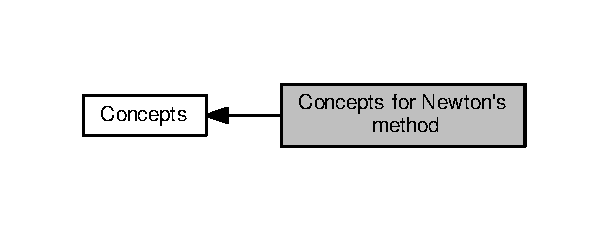
\includegraphics[width=292pt]{group__NewtonConceptGroup}
\end{center}
\end{figure}
\subsection*{Typedefs}
\begin{DoxyCompactItemize}
\item 
using \hyperlink{group__NewtonConceptGroup_ga8da917ba6de9c283c1509281956bb04a_ga8da917ba6de9c283c1509281956bb04a}{Spacy\+::\+Concepts\+::\+Newton\+::\+Damping\+Strategy\+Concept} = boost\+::mpl\+::vector$<$ \+::\hyperlink{group__ConceptGroup_ga63426675cc05ccce03ead56a4fa90d96_ga63426675cc05ccce03ead56a4fa90d96}{Spacy\+::\+Concepts\+::\+Concept\+Base}, boost\+::type\+\_\+erasure\+::callable$<$ \+::\hyperlink{classSpacy_1_1DampingFactor}{Spacy\+::\+Damping\+Factor}(const boost\+::type\+\_\+erasure\+::any$<$ \+::\hyperlink{group__ConceptGroup_gac7d6a94c7131c8613e2ab26fddeb50bd_gac7d6a94c7131c8613e2ab26fddeb50bd}{Spacy\+::\+Concepts\+::\+Linear\+Solver\+Concept} $>$ \&, const Vector \&, const Vector \&), const boost\+::type\+\_\+erasure\+::\+\_\+self $>$ $>$
\begin{DoxyCompactList}\small\item\em Concept for damping strategies for Newton\textquotesingle{}s method. \end{DoxyCompactList}\item 
using \hyperlink{group__NewtonConceptGroup_ga7d7604bea8b7c261d3179a7e95ffbe76_ga7d7604bea8b7c261d3179a7e95ffbe76}{Spacy\+::\+Concepts\+::\+Newton\+::\+Termination\+Criterion\+Concept} = boost\+::mpl\+::vector$<$ \+::\hyperlink{group__ConceptGroup_ga63426675cc05ccce03ead56a4fa90d96_ga63426675cc05ccce03ead56a4fa90d96}{Spacy\+::\+Concepts\+::\+Concept\+Base}, boost\+::type\+\_\+erasure\+::callable$<$ bool(Damping\+Factor, const Vector \&, const Vector \&), const boost\+::type\+\_\+erasure\+::\+\_\+self $>$ $>$
\begin{DoxyCompactList}\small\item\em Concept for termination criteria for Newton\textquotesingle{}s method. \end{DoxyCompactList}\end{DoxyCompactItemize}


\subsection{Detailed Description}
Concepts for damping strategy and termination criteria for Newton\textquotesingle{}s method. 



\subsection{Typedef Documentation}
\hypertarget{group__NewtonConceptGroup_ga8da917ba6de9c283c1509281956bb04a_ga8da917ba6de9c283c1509281956bb04a}{}\index{Concepts for Newton\textquotesingle{}s method@{Concepts for Newton\textquotesingle{}s method}!Damping\+Strategy\+Concept@{Damping\+Strategy\+Concept}}
\index{Damping\+Strategy\+Concept@{Damping\+Strategy\+Concept}!Concepts for Newton\textquotesingle{}s method@{Concepts for Newton\textquotesingle{}s method}}
\subsubsection[{Damping\+Strategy\+Concept}]{\setlength{\rightskip}{0pt plus 5cm}using {\bf Spacy\+::\+Concepts\+::\+Newton\+::\+Damping\+Strategy\+Concept} = typedef boost\+::mpl\+::vector$<$ \+::{\bf Spacy\+::\+Concepts\+::\+Concept\+Base} , boost\+::type\+\_\+erasure\+::callable$<$ \+::{\bf Spacy\+::\+Damping\+Factor}(const boost\+::type\+\_\+erasure\+::any$<$ \+::{\bf Spacy\+::\+Concepts\+::\+Linear\+Solver\+Concept} $>$\&, const Vector\&, const Vector\&), const boost\+::type\+\_\+erasure\+::\+\_\+self$>$ $>$}\label{group__NewtonConceptGroup_ga8da917ba6de9c283c1509281956bb04a_ga8da917ba6de9c283c1509281956bb04a}


Concept for damping strategies for Newton\textquotesingle{}s method. 

\label{group__NewtonConceptGroup_ga8da917ba6de9c283c1509281956bb04a_Newton_DampingStrategyConceptAnchor}%
\hypertarget{group__NewtonConceptGroup_ga8da917ba6de9c283c1509281956bb04a_Newton_DampingStrategyConceptAnchor}{}%
The minimal signature of a damping strategy is\+: 
\begin{DoxyCode}
\textcolor{comment}{// My damping strategy.}
\textcolor{keyword}{class }MyDampingStrategy
\{
\textcolor{keyword}{public}:
  \textcolor{comment}{// Copy constructor.}
  MyDampingStrategy(\textcolor{keyword}{const} MyDampingStrategy&);

  \textcolor{comment}{// Move constructor.}
  MyDampingStrategy(MyDampingStrategy&&);

  \textcolor{comment}{// Compute damping factor.}
  DampingFactor operator()(\textcolor{keyword}{const} \hyperlink{namespaceSpacy_a7d5cd1c6fb9dd85aa345b536caf30bba_a7d5cd1c6fb9dd85aa345b536caf30bba}{LinearSolver}& DF\_inv, \textcolor{keyword}{const} Vector& x, \textcolor{keyword}{const} Vector& dx) \textcolor{keyword}{const}
      ;
\};
\end{DoxyCode}


\begin{DoxySeeAlso}{See also}
\hyperlink{namespaceSpacy_1_1Newton_ae2ba8821b209bfac2ab9190e6283cf06_Newton_DampingStrategyAnchor}{Newton\+:\+:Damping\+Strategy}, \hyperlink{namespaceSpacy_a7d5cd1c6fb9dd85aa345b536caf30bba_LinearSolverAnchor}{Linear\+Solver}, \hyperlink{group__SpacyGroup_gafc144d2730ef87a67e54f8cd750b1f54_VectorAnchor}{Vector}, \hyperlink{classSpacy_1_1DampingFactor}{Damping\+Factor} 
\end{DoxySeeAlso}
\hypertarget{group__NewtonConceptGroup_ga7d7604bea8b7c261d3179a7e95ffbe76_ga7d7604bea8b7c261d3179a7e95ffbe76}{}\index{Concepts for Newton\textquotesingle{}s method@{Concepts for Newton\textquotesingle{}s method}!Termination\+Criterion\+Concept@{Termination\+Criterion\+Concept}}
\index{Termination\+Criterion\+Concept@{Termination\+Criterion\+Concept}!Concepts for Newton\textquotesingle{}s method@{Concepts for Newton\textquotesingle{}s method}}
\subsubsection[{Termination\+Criterion\+Concept}]{\setlength{\rightskip}{0pt plus 5cm}using {\bf Spacy\+::\+Concepts\+::\+Newton\+::\+Termination\+Criterion\+Concept} = typedef boost\+::mpl\+::vector$<$ \+::{\bf Spacy\+::\+Concepts\+::\+Concept\+Base} , boost\+::type\+\_\+erasure\+::callable$<$bool(Damping\+Factor, const Vector\&, const Vector\&), const boost\+::type\+\_\+erasure\+::\+\_\+self$>$ $>$}\label{group__NewtonConceptGroup_ga7d7604bea8b7c261d3179a7e95ffbe76_ga7d7604bea8b7c261d3179a7e95ffbe76}


Concept for termination criteria for Newton\textquotesingle{}s method. 

\label{group__NewtonConceptGroup_ga7d7604bea8b7c261d3179a7e95ffbe76_Newton_TerminationCriterionConceptAnchor}%
\hypertarget{group__NewtonConceptGroup_ga7d7604bea8b7c261d3179a7e95ffbe76_Newton_TerminationCriterionConceptAnchor}{}%
The minimal signature of a termination criterion is\+: 
\begin{DoxyCode}
\textcolor{comment}{// My termination criterion.}
\textcolor{keyword}{class }MyTerminationCriterion
\{
\textcolor{keyword}{public}:
  \textcolor{comment}{// Copy constructor.}
  MyTerminationCriterion(\textcolor{keyword}{const} MyTerminationCriterion&);

  \textcolor{comment}{// Move constructor.}
  MyTerminationCriterion(MyTerminationCriterion&&);

  \textcolor{comment}{// Check if termination criterion is satisfied.}
  \textcolor{keywordtype}{bool} operator()(DampingFactor nu, \textcolor{keyword}{const} Vector& x, \textcolor{keyword}{const} Vector& dx) \textcolor{keyword}{const};
\};
\end{DoxyCode}


\begin{DoxySeeAlso}{See also}
\hyperlink{namespaceSpacy_1_1Newton_abfa64b52531032d7a5fe6d0ec1a3cbd5_Newton_TerminationCriterionAnchor}{Newton\+:\+:Termination\+Criterion}, \hyperlink{group__SpacyGroup_gafc144d2730ef87a67e54f8cd750b1f54_VectorAnchor}{Vector} 
\end{DoxySeeAlso}

\hypertarget{group__CGConceptGroup}{}\section{Concepts for conjugate gradient methods}
\label{group__CGConceptGroup}\index{Concepts for conjugate gradient methods@{Concepts for conjugate gradient methods}}


Concept for termination criteria for conjugate gradient methods.  


Collaboration diagram for Concepts for conjugate gradient methods\+:\nopagebreak
\begin{figure}[H]
\begin{center}
\leavevmode
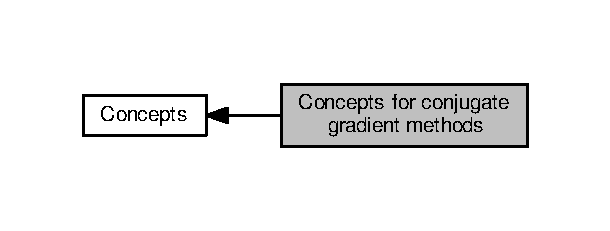
\includegraphics[width=293pt]{group__CGConceptGroup}
\end{center}
\end{figure}
\subsection*{Typedefs}
\begin{DoxyCompactItemize}
\item 
using \hyperlink{group__CGConceptGroup_ga6b30d103c365816efcfb038d922aef07_ga6b30d103c365816efcfb038d922aef07}{Spacy\+::\+Concepts\+::\+C\+G\+::\+Termination\+Criterion\+Concept} = boost\+::mpl\+::vector$<$ Concept\+Base, boost\+::type\+\_\+erasure\+::callable$<$ bool(), const boost\+::type\+\_\+erasure\+::\+\_\+self $>$, has\+\_\+cg\+\_\+terminate\+\_\+clear$<$ void()$>$, has\+\_\+cg\+\_\+terminate\+\_\+update$<$ void(Real, Real, Real, Real)$>$, has\+\_\+cg\+\_\+terminate\+\_\+vanishing\+Step$<$ bool(), const boost\+::type\+\_\+erasure\+::\+\_\+self $>$, has\+\_\+cg\+\_\+terminate\+\_\+minimal\+Decrease\+Achieved$<$ bool(), const boost\+::type\+\_\+erasure\+::\+\_\+self $>$, has\+\_\+cg\+\_\+terminate\+\_\+set\+Eps$<$ void(double)$>$, has\+\_\+cg\+\_\+terminate\+\_\+set\+Relative\+Accuracy$<$ void(double)$>$, has\+\_\+cg\+\_\+terminate\+\_\+set\+Absolute\+Accuracy$<$ void(double)$>$, has\+\_\+cg\+\_\+terminate\+\_\+set\+Minimal\+Accuracy$<$ void(double)$>$ $>$
\begin{DoxyCompactList}\small\item\em Concept for termination criteria for conjugate gradient methods. \end{DoxyCompactList}\end{DoxyCompactItemize}


\subsection{Detailed Description}
Concept for termination criteria for conjugate gradient methods. 



\subsection{Typedef Documentation}
\hypertarget{group__CGConceptGroup_ga6b30d103c365816efcfb038d922aef07_ga6b30d103c365816efcfb038d922aef07}{}\index{Concepts for conjugate gradient methods@{Concepts for conjugate gradient methods}!Termination\+Criterion\+Concept@{Termination\+Criterion\+Concept}}
\index{Termination\+Criterion\+Concept@{Termination\+Criterion\+Concept}!Concepts for conjugate gradient methods@{Concepts for conjugate gradient methods}}
\subsubsection[{Termination\+Criterion\+Concept}]{\setlength{\rightskip}{0pt plus 5cm}using {\bf Spacy\+::\+Concepts\+::\+C\+G\+::\+Termination\+Criterion\+Concept} = typedef boost\+::mpl\+::vector$<$ Concept\+Base , boost\+::type\+\_\+erasure\+::callable$<$bool(), const boost\+::type\+\_\+erasure\+::\+\_\+self$>$ , has\+\_\+cg\+\_\+terminate\+\_\+clear$<$void()$>$ , has\+\_\+cg\+\_\+terminate\+\_\+update$<$void(Real,Real,Real,Real)$>$ , has\+\_\+cg\+\_\+terminate\+\_\+vanishing\+Step$<$bool(), const boost\+::type\+\_\+erasure\+::\+\_\+self$>$ , has\+\_\+cg\+\_\+terminate\+\_\+minimal\+Decrease\+Achieved$<$bool(), const boost\+::type\+\_\+erasure\+::\+\_\+self$>$ , has\+\_\+cg\+\_\+terminate\+\_\+set\+Eps$<$void(double)$>$ , has\+\_\+cg\+\_\+terminate\+\_\+set\+Relative\+Accuracy$<$void(double)$>$ , has\+\_\+cg\+\_\+terminate\+\_\+set\+Absolute\+Accuracy$<$void(double)$>$ , has\+\_\+cg\+\_\+terminate\+\_\+set\+Minimal\+Accuracy$<$void(double)$>$ $>$}\label{group__CGConceptGroup_ga6b30d103c365816efcfb038d922aef07_ga6b30d103c365816efcfb038d922aef07}


Concept for termination criteria for conjugate gradient methods. 

\label{group__CGConceptGroup_ga6b30d103c365816efcfb038d922aef07_CG_TerminationCriterionConceptAnchor}%
\hypertarget{group__CGConceptGroup_ga6b30d103c365816efcfb038d922aef07_CG_TerminationCriterionConceptAnchor}{}%
The minimal signature of a termination criterion is\+: 
\begin{DoxyCode}
\textcolor{comment}{// My termination criterion.}
\textcolor{keyword}{class }MyTerminationCriterion
\{
\textcolor{keyword}{public}:
  \textcolor{comment}{// Copy constructor.}
  MyTerminationCriterion(\textcolor{keyword}{const} MyTerminationCriterion&);

  \textcolor{comment}{// Move constructor.}
  MyTerminationCriterion(MyTerminationCriterion&&);

  \textcolor{comment}{// Check if termination criterion is satisfied.}
  \textcolor{keywordtype}{bool} operator()() \textcolor{keyword}{const};

  \textcolor{comment}{// Clear internal storage for new cg run.}
  \textcolor{keywordtype}{void} clear();

  \textcolor{comment}{// Provide algorithmic quantities required to evaluate termination criteria.}
  \textcolor{keywordtype}{void} update(Real stepLength, Real qAq, Real qPq, Real rPINVr)

  \textcolor{comment}{// Checks if the step length of the computed step is below the maximal attainable accuracy.}
  \textcolor{keywordtype}{bool} vanishingStep() \textcolor{keyword}{const};

  \textcolor{comment}{// Checks if at least the minimal required decrease is satisfied. This is required for the}
  \textcolor{comment}{// truncated regularized conjugate gradient method (TRCG).}
  \textcolor{keywordtype}{bool} minimalDecreaseAchieved() \textcolor{keyword}{const};

  \textcolor{comment}{// Set maximal attainable accuracy}
  \textcolor{keywordtype}{void} setEps(\textcolor{keywordtype}{double});

  \textcolor{comment}{// Set relative accuracy.}
  \textcolor{keywordtype}{void} setRelativeAccuracy(\textcolor{keywordtype}{double});

  \textcolor{comment}{// Set absolute accuracy.}
  \textcolor{keywordtype}{void} setAbsoluteAccuracy(\textcolor{keywordtype}{double});

  \textcolor{comment}{// Set minimal accuracy. Only required for truncated regularized conjugate gradients (TRCG).}
  \textcolor{keywordtype}{void} setMinimalAccuracy(\textcolor{keywordtype}{double});
\};
\end{DoxyCode}


\begin{DoxySeeAlso}{See also}
\hyperlink{group__CGGroup_gaa927be31b313bb4ce635668c77b55860_CG_TerminationCriterionAnchor}{C\+G\+:\+:Termination\+Criterion} 
\end{DoxySeeAlso}

\chapter{Namespace Documentation}
\hypertarget{namespaceAlgorithm_1_1CG}{}\section{Algorithm\+:\+:C\+G Namespace Reference}
\label{namespaceAlgorithm_1_1CG}\index{Algorithm\+::\+C\+G@{Algorithm\+::\+C\+G}}


Conjugate gradient methods for convex and nonconvex problems (C\+G, Truncated C\+G, Regularized C\+G and Truncated Regularized C\+G).  


\subsection*{Namespaces}
\begin{DoxyCompactItemize}
\item 
 \hyperlink{namespaceAlgorithm_1_1CG_1_1Termination}{Termination}
\begin{DoxyCompactList}\small\item\em \hyperlink{namespaceAlgorithm_1_1CG_1_1Termination}{Termination} criteria for conjugate gradient methods. \end{DoxyCompactList}\end{DoxyCompactItemize}


\subsection{Detailed Description}
Conjugate gradient methods for convex and nonconvex problems (C\+G, Truncated C\+G, Regularized C\+G and Truncated Regularized C\+G). 

\begin{DoxySeeAlso}{See also}
\hyperlink{group__CGGroup}{Conjugate Gradient Methods}, \hyperlink{group__CGConceptGroup}{Concepts for conjugate gradient methods} 
\end{DoxySeeAlso}

\hypertarget{namespaceAlgorithm_1_1CG_1_1Termination}{}\section{Algorithm\+:\+:C\+G\+:\+:Termination Namespace Reference}
\label{namespaceAlgorithm_1_1CG_1_1Termination}\index{Algorithm\+::\+C\+G\+::\+Termination@{Algorithm\+::\+C\+G\+::\+Termination}}


\hyperlink{namespaceAlgorithm_1_1CG_1_1Termination}{Termination} criteria for conjugate gradient methods.  




\subsection{Detailed Description}
\hyperlink{namespaceAlgorithm_1_1CG_1_1Termination}{Termination} criteria for conjugate gradient methods. 

\begin{DoxySeeAlso}{See also}
\hyperlink{group__CGGroup}{Conjugate Gradient Methods}, \hyperlink{group__CGConceptGroup}{Concepts for conjugate gradient methods} 
\end{DoxySeeAlso}

\hypertarget{namespaceAlgorithm_1_1Concepts}{}\section{Algorithm\+:\+:Concepts Namespace Reference}
\label{namespaceAlgorithm_1_1Concepts}\index{Algorithm\+::\+Concepts@{Algorithm\+::\+Concepts}}


Concepts for vectors, functional, operators, ...  


\subsection*{Namespaces}
\begin{DoxyCompactItemize}
\item 
 \hyperlink{namespaceAlgorithm_1_1Concepts_1_1CG}{C\+G}
\begin{DoxyCompactList}\small\item\em Concept for termination criteria for conjugate gradient methods. \end{DoxyCompactList}\item 
 \hyperlink{namespaceAlgorithm_1_1Concepts_1_1CompositeStep}{Composite\+Step}
\begin{DoxyCompactList}\small\item\em Contains the affine covariant composite step method of \cite{Lubkoll2015}, \cite{Lubkoll2015a}. \end{DoxyCompactList}\item 
 \hyperlink{namespaceAlgorithm_1_1Concepts_1_1Newton}{Newton}
\begin{DoxyCompactList}\small\item\em Concepts for damping strategy and termination criteria for Newton\textquotesingle{}s method. \end{DoxyCompactList}\end{DoxyCompactItemize}


\subsection{Detailed Description}
Concepts for vectors, functional, operators, ... 

\begin{DoxySeeAlso}{See also}
\hyperlink{group__ConceptGroup}{Concepts} 
\end{DoxySeeAlso}

\hypertarget{namespaceAlgorithm_1_1Concepts_1_1CG}{}\section{Algorithm\+:\+:Concepts\+:\+:C\+G Namespace Reference}
\label{namespaceAlgorithm_1_1Concepts_1_1CG}\index{Algorithm\+::\+Concepts\+::\+C\+G@{Algorithm\+::\+Concepts\+::\+C\+G}}


Concept for termination criteria for conjugate gradient methods.  




\subsection{Detailed Description}
Concept for termination criteria for conjugate gradient methods. 

\begin{DoxySeeAlso}{See also}
\hyperlink{group__CGConceptGroup}{Concepts for conjugate gradient methods} 
\end{DoxySeeAlso}

\hypertarget{namespaceAlgorithm_1_1Concepts_1_1CompositeStep}{}\section{Algorithm\+:\+:Concepts\+:\+:Composite\+Step Namespace Reference}
\label{namespaceAlgorithm_1_1Concepts_1_1CompositeStep}\index{Algorithm\+::\+Concepts\+::\+Composite\+Step@{Algorithm\+::\+Concepts\+::\+Composite\+Step}}


Contains the affine covariant composite step method of \cite{Lubkoll2015}, \cite{Lubkoll2015a}.  




\subsection{Detailed Description}
Contains the affine covariant composite step method of \cite{Lubkoll2015}, \cite{Lubkoll2015a}. 

\begin{DoxySeeAlso}{See also}
\hyperlink{group__CSGroup}{Composite Step Methods} 
\end{DoxySeeAlso}

\hypertarget{namespaceAlgorithm_1_1Concepts_1_1Newton}{}\section{Algorithm\+:\+:Concepts\+:\+:Newton Namespace Reference}
\label{namespaceAlgorithm_1_1Concepts_1_1Newton}\index{Algorithm\+::\+Concepts\+::\+Newton@{Algorithm\+::\+Concepts\+::\+Newton}}


Concepts for damping strategy and termination criteria for Newton\textquotesingle{}s method.  




\subsection{Detailed Description}
Concepts for damping strategy and termination criteria for Newton\textquotesingle{}s method. 

\begin{DoxySeeAlso}{See also}
\hyperlink{group__NewtonConceptGroup}{Concepts for Newton\textquotesingle{}s method} 
\end{DoxySeeAlso}

\hypertarget{namespaceAlgorithm_1_1FEniCS}{}\section{Algorithm\+:\+:F\+Eni\+C\+S Namespace Reference}
\label{namespaceAlgorithm_1_1FEniCS}\index{Algorithm\+::\+F\+Eni\+C\+S@{Algorithm\+::\+F\+Eni\+C\+S}}


Contains vector spaces, functionals and operators for \href{www.fenicsproject.org}{\tt F\+Eni\+C\+S}.  




\subsection{Detailed Description}
Contains vector spaces, functionals and operators for \href{www.fenicsproject.org}{\tt F\+Eni\+C\+S}. 

\begin{DoxySeeAlso}{See also}
\hyperlink{group__FenicsGroup}{Vector Space for F\+Eni\+C\+S} 
\end{DoxySeeAlso}

\hypertarget{namespaceAlgorithm_1_1Kaskade}{}\section{Algorithm\+:\+:Kaskade Namespace Reference}
\label{namespaceAlgorithm_1_1Kaskade}\index{Algorithm\+::\+Kaskade@{Algorithm\+::\+Kaskade}}


Contains vector spaces, functionals and operators for \href{http://www.zib.de/projects/kaskade7-finite-element-toolbox}{\tt Kaskade 7}.  




\subsection{Detailed Description}
Contains vector spaces, functionals and operators for \href{http://www.zib.de/projects/kaskade7-finite-element-toolbox}{\tt Kaskade 7}. 

\begin{DoxySeeAlso}{See also}
\hyperlink{group__KaskadeGroup}{Vector Space for Kaskade 7} 
\end{DoxySeeAlso}

\hypertarget{namespaceAlgorithm_1_1Mixin}{}\section{Algorithm\+:\+:Mixin Namespace Reference}
\label{namespaceAlgorithm_1_1Mixin}\index{Algorithm\+::\+Mixin@{Algorithm\+::\+Mixin}}


Contains components that are frequently used and can be added to your classes via (multiple) inheritance.  




\subsection{Detailed Description}
Contains components that are frequently used and can be added to your classes via (multiple) inheritance. 

\begin{DoxySeeAlso}{See also}
\hyperlink{group__MixinGroup}{Mixins} 
\end{DoxySeeAlso}

\hypertarget{namespaceAlgorithm_1_1Newton}{}\section{Algorithm\+:\+:Newton Namespace Reference}
\label{namespaceAlgorithm_1_1Newton}\index{Algorithm\+::\+Newton@{Algorithm\+::\+Newton}}


Newton methods, largely following \cite{Deuflhard2004}.  


\subsection*{Namespaces}
\begin{DoxyCompactItemize}
\item 
 \hyperlink{namespaceAlgorithm_1_1Newton_1_1Damping}{Damping}
\begin{DoxyCompactList}\small\item\em \hyperlink{namespaceAlgorithm_1_1Newton_1_1Damping}{Damping} strategies for \hyperlink{namespaceAlgorithm_1_1Newton}{Newton}\textquotesingle{}s method. \end{DoxyCompactList}\item 
 \hyperlink{namespaceAlgorithm_1_1Newton_1_1Termination}{Termination}
\begin{DoxyCompactList}\small\item\em \hyperlink{namespaceAlgorithm_1_1Newton_1_1Termination}{Termination} criteria for \hyperlink{namespaceAlgorithm_1_1Newton}{Newton}\textquotesingle{}s method. \end{DoxyCompactList}\end{DoxyCompactItemize}


\subsection{Detailed Description}
Newton methods, largely following \cite{Deuflhard2004}. 

Contains a local Newton method, an affine covariant Newton method, an affine contravariant Newton method as well as a generic implementation that admits the implementation of further termination criteria and damping strategies. \begin{DoxySeeAlso}{See also}
\hyperlink{group__NewtonGroup}{Newton Methods}, \hyperlink{group__NewtonConceptGroup}{Concepts for Newton\textquotesingle{}s method} 
\end{DoxySeeAlso}

\hypertarget{namespaceAlgorithm_1_1Newton_1_1Damping}{}\section{Algorithm\+:\+:Newton\+:\+:Damping Namespace Reference}
\label{namespaceAlgorithm_1_1Newton_1_1Damping}\index{Algorithm\+::\+Newton\+::\+Damping@{Algorithm\+::\+Newton\+::\+Damping}}


\hyperlink{namespaceAlgorithm_1_1Newton_1_1Damping}{Damping} strategies for \hyperlink{namespaceAlgorithm_1_1Newton}{Newton}\textquotesingle{}s method.  




\subsection{Detailed Description}
\hyperlink{namespaceAlgorithm_1_1Newton_1_1Damping}{Damping} strategies for \hyperlink{namespaceAlgorithm_1_1Newton}{Newton}\textquotesingle{}s method. 

\begin{DoxySeeAlso}{See also}
\hyperlink{group__NewtonGroup}{Newton Methods}, \hyperlink{group__NewtonConceptGroup}{Concepts for Newton\textquotesingle{}s method} 
\end{DoxySeeAlso}

\hypertarget{namespaceAlgorithm_1_1Newton_1_1Termination}{}\section{Algorithm\+:\+:Newton\+:\+:Termination Namespace Reference}
\label{namespaceAlgorithm_1_1Newton_1_1Termination}\index{Algorithm\+::\+Newton\+::\+Termination@{Algorithm\+::\+Newton\+::\+Termination}}


\hyperlink{namespaceAlgorithm_1_1Newton_1_1Termination}{Termination} criteria for \hyperlink{namespaceAlgorithm_1_1Newton}{Newton}\textquotesingle{}s method.  




\subsection{Detailed Description}
\hyperlink{namespaceAlgorithm_1_1Newton_1_1Termination}{Termination} criteria for \hyperlink{namespaceAlgorithm_1_1Newton}{Newton}\textquotesingle{}s method. 

\begin{DoxySeeAlso}{See also}
\hyperlink{group__NewtonGroup}{Newton Methods}, \hyperlink{group__NewtonConceptGroup}{Concepts for Newton\textquotesingle{}s method} 
\end{DoxySeeAlso}

\hypertarget{namespaceAlgorithm_1_1ProductSpace}{}\section{Algorithm\+:\+:Product\+Space Namespace Reference}
\label{namespaceAlgorithm_1_1ProductSpace}\index{Algorithm\+::\+Product\+Space@{Algorithm\+::\+Product\+Space}}


A product space that supports distinction between primal and dual variables.  




\subsection{Detailed Description}
A product space that supports distinction between primal and dual variables. 

\begin{DoxySeeAlso}{See also}
\hyperlink{group__ProductSpaceGroup}{Product Space} 
\end{DoxySeeAlso}

\hypertarget{namespaceAlgorithm_1_1RealSpace}{}\section{Algorithm\+:\+:Real\+Space Namespace Reference}
\label{namespaceAlgorithm_1_1RealSpace}\index{Algorithm\+::\+Real\+Space@{Algorithm\+::\+Real\+Space}}


A one dimensional vector space representing the space of real numbers.  




\subsection{Detailed Description}
A one dimensional vector space representing the space of real numbers. 

\begin{DoxySeeAlso}{See also}
\hyperlink{group__RealGroup}{Real Space} 
\end{DoxySeeAlso}

\hypertarget{namespaceSpacy}{}\section{Spacy Namespace Reference}
\label{namespaceSpacy}\index{Spacy@{Spacy}}


Main namespace of the Spacy library.  


\subsection*{Namespaces}
\begin{DoxyCompactItemize}
\item 
 \hyperlink{namespaceSpacy_1_1CG}{C\+G}
\begin{DoxyCompactList}\small\item\em Conjugate gradient methods for convex and nonconvex problems (C\+G, Truncated C\+G, Regularized C\+G and Truncated Regularized C\+G). \end{DoxyCompactList}\item 
 \hyperlink{namespaceSpacy_1_1Concepts}{Concepts}
\begin{DoxyCompactList}\small\item\em Concepts for vectors, functional, operators, ... \end{DoxyCompactList}\item 
 \hyperlink{namespaceSpacy_1_1FEniCS}{F\+Eni\+C\+S}
\begin{DoxyCompactList}\small\item\em Contains vector spaces, functionals and operators for \href{www.fenicsproject.org}{\tt F\+Eni\+C\+S}. \end{DoxyCompactList}\item 
 \hyperlink{namespaceSpacy_1_1Kaskade}{Kaskade}
\begin{DoxyCompactList}\small\item\em Contains vector spaces, functionals and operators for \href{http://www.zib.de/projects/kaskade7-finite-element-toolbox}{\tt Kaskade 7}. \end{DoxyCompactList}\item 
 \hyperlink{namespaceSpacy_1_1Mixin}{Mixin}
\begin{DoxyCompactList}\small\item\em Contains components that are frequently used and can be added to your classes via (multiple) inheritance. \end{DoxyCompactList}\item 
 \hyperlink{namespaceSpacy_1_1Newton}{Newton}
\begin{DoxyCompactList}\small\item\em Newton methods, largely following \cite{Deuflhard2004}. \end{DoxyCompactList}\item 
 \hyperlink{namespaceSpacy_1_1ProductSpace}{Product\+Space}
\begin{DoxyCompactList}\small\item\em A product space that supports distinction between primal and dual variables. \end{DoxyCompactList}\item 
 \hyperlink{namespaceSpacy_1_1RealSpace}{Real\+Space}
\begin{DoxyCompactList}\small\item\em A one dimensional vector space representing the space of real numbers. \end{DoxyCompactList}\end{DoxyCompactItemize}
\subsection*{Classes}
\begin{DoxyCompactItemize}
\item 
class \hyperlink{classSpacy_1_1C2FunctionalBase}{C2\+Functional\+Base}
\begin{DoxyCompactList}\small\item\em Base class for twice differentiable functionals $ f:\ X\rightarrow \mathbb{R}$. \end{DoxyCompactList}\item 
class \hyperlink{classSpacy_1_1CallOfUndefinedFunctionException}{Call\+Of\+Undefined\+Function\+Exception}
\begin{DoxyCompactList}\small\item\em Exception to be thrown if a virtual function is not implemented. \end{DoxyCompactList}\item 
class \hyperlink{classSpacy_1_1DampingFactor}{Damping\+Factor}
\begin{DoxyCompactList}\small\item\em A simple model of a damping factor $\nu$ that is computed up to a prescribed accuracy $\varepsilon$. \end{DoxyCompactList}\item 
class \hyperlink{classSpacy_1_1GenericException}{Generic\+Exception}
\begin{DoxyCompactList}\small\item\em A generic exception class that serves as base for all exceptions in this library. \end{DoxyCompactList}\item 
class \hyperlink{classSpacy_1_1Hessian}{Hessian}
\begin{DoxyCompactList}\small\item\em Linear operator $f''(x)$ for a twice differentiable functional $f$. \end{DoxyCompactList}\item 
class \hyperlink{classSpacy_1_1IncompatibleSpaceException}{Incompatible\+Space\+Exception}
\begin{DoxyCompactList}\small\item\em Exception to be thrown when encountering incompatible spaces. \end{DoxyCompactList}\item 
class \hyperlink{classSpacy_1_1InducedScalarProduct}{Induced\+Scalar\+Product}
\begin{DoxyCompactList}\small\item\em Induced scalar product $(x,y)_M = (Mx)y$, where $M:X\rightarrow X^*$. \end{DoxyCompactList}\item 
class \hyperlink{classSpacy_1_1InvalidArgumentException}{Invalid\+Argument\+Exception}
\begin{DoxyCompactList}\small\item\em Exception to be thrown on invalid arguments. \end{DoxyCompactList}\item 
class \hyperlink{classSpacy_1_1LinearizedOperator}{Linearized\+Operator}
\begin{DoxyCompactList}\small\item\em Linearized operator $A'(x)$ of a differentiable operator $A$. \end{DoxyCompactList}\item 
class \hyperlink{classSpacy_1_1LipschitzConstant}{Lipschitz\+Constant}
\begin{DoxyCompactList}\small\item\em A simple model for a Lipschitz constant $\omega$. \end{DoxyCompactList}\item 
class \hyperlink{classSpacy_1_1OperatorBase}{Operator\+Base}
\begin{DoxyCompactList}\small\item\em Base class for operators $A:\ X\rightarrow Y$, between function spaces $X$ and $Y$. \end{DoxyCompactList}\item 
class \hyperlink{classSpacy_1_1Parameter}{Parameter}
\begin{DoxyCompactList}\small\item\em Basic parameters for simple algorithms. \end{DoxyCompactList}\item 
class \hyperlink{classSpacy_1_1PrimalInducedScalarProduct}{Primal\+Induced\+Scalar\+Product}
\begin{DoxyCompactList}\small\item\em Induced scalar product for the primal variables (i.\+e. for constrained optimization problems). \end{DoxyCompactList}\item 
class \hyperlink{classSpacy_1_1Real}{Real}
\begin{DoxyCompactList}\small\item\em \hyperlink{classSpacy_1_1Real}{Real} number. \end{DoxyCompactList}\item 
class \hyperlink{classSpacy_1_1RegularityTestFailedException}{Regularity\+Test\+Failed\+Exception}
\begin{DoxyCompactList}\small\item\em Exception to be thrown if regularity test fails. \end{DoxyCompactList}\item 
class \hyperlink{classSpacy_1_1SingularOperatorException}{Singular\+Operator\+Exception}
\begin{DoxyCompactList}\small\item\em Exception to be thrown if singular operators are inverted. \end{DoxyCompactList}\item 
class \hyperlink{classSpacy_1_1SupportedOperatorBase}{Supported\+Operator\+Base}
\begin{DoxyCompactList}\small\item\em Base class providing some operations for vectors via C\+R\+T\+P. \end{DoxyCompactList}\item 
class \hyperlink{classSpacy_1_1Vector}{Vector}
\item 
class \hyperlink{classSpacy_1_1VectorBase}{Vector\+Base}
\begin{DoxyCompactList}\small\item\em Base class for vector implementations. \end{DoxyCompactList}\item 
class \hyperlink{classSpacy_1_1VectorSpace}{Vector\+Space}
\begin{DoxyCompactList}\small\item\em Function space $(X,\|\cdot\|)$. \end{DoxyCompactList}\end{DoxyCompactItemize}
\subsection*{Typedefs}
\begin{DoxyCompactItemize}
\item 
using \hyperlink{group__SpacyGroup_ga750d55072f7a3a16a1263961147333c0_ga750d55072f7a3a16a1263961147333c0}{Dynamic\+Callable\+Operator} = boost\+::type\+\_\+erasure\+::any$<$ \hyperlink{group__ConceptGroup_ga30692db093ead5a1a074905363a2f043_ga30692db093ead5a1a074905363a2f043}{Concepts\+::\+Dynamic\+Callable\+Operator\+Concept} $>$
\begin{DoxyCompactList}\small\item\em Simplest possible time-\/dependent operator. Can store objects that satisfy the requirements of \hyperlink{group__ConceptGroup_ga30692db093ead5a1a074905363a2f043_DynamicCallableOperatorConceptAnchor}{Dynamic\+Callable\+Operator\+Concept}. \end{DoxyCompactList}\item 
using \hyperlink{group__SpacyGroup_gaad10aa7d5443703377b768fa41a3c7ea_gaad10aa7d5443703377b768fa41a3c7ea}{Dynamic\+Linear\+Operator} = boost\+::type\+\_\+erasure\+::any$<$ \hyperlink{group__ConceptGroup_ga015b0d099011a2ef73a16aa9b36a7346_ga015b0d099011a2ef73a16aa9b36a7346}{Concepts\+::\+Dynamic\+Linear\+Operator\+Concept} $>$
\begin{DoxyCompactList}\small\item\em Time-\/dependent linear operator class. Can store objects that satisfy the requirements of \hyperlink{group__ConceptGroup_ga015b0d099011a2ef73a16aa9b36a7346_DynamicLinearOperatorConceptAnchor}{Dynamic\+Linear\+Operator\+Concept}. \end{DoxyCompactList}\item 
using \hyperlink{group__SpacyGroup_ga8e692134dfe46346d5692acfd1a9bd8e_ga8e692134dfe46346d5692acfd1a9bd8e}{Dynamic\+Operator} = boost\+::type\+\_\+erasure\+::any$<$ \hyperlink{group__ConceptGroup_ga2c979d268f0ca7a436776a9631d10af7_ga2c979d268f0ca7a436776a9631d10af7}{Concepts\+::\+Dynamic\+Operator\+Concept} $>$
\begin{DoxyCompactList}\small\item\em Time-\/dependent operator. Can store objects that satisfy the requirements of \hyperlink{group__ConceptGroup_ga2c979d268f0ca7a436776a9631d10af7_DynamicOperatorConceptAnchor}{Dynamic\+Operator\+Concept}. \end{DoxyCompactList}\item 
using \hyperlink{group__SpacyGroup_gabc9c830d2a7e020bcab097b10ee6f642_gabc9c830d2a7e020bcab097b10ee6f642}{Dynamic\+C1\+Operator} = boost\+::type\+\_\+erasure\+::any$<$ \hyperlink{group__ConceptGroup_gaa7ef0ce2d66b0610035541b580564b11_gaa7ef0ce2d66b0610035541b580564b11}{Concepts\+::\+Dynamic\+C1\+Operator\+Concept} $>$
\begin{DoxyCompactList}\small\item\em Time-\/dependent differentiable operator. Can store objects that satisfy the requirements of \hyperlink{group__ConceptGroup_gaa7ef0ce2d66b0610035541b580564b11_DynamicC1OperatorConceptAnchor}{Dynamic\+C1\+Operator\+Concept}. \end{DoxyCompactList}\item 
using \hyperlink{group__SpacyGroup_ga673218f603c93790864aef12c89d3a35_ga673218f603c93790864aef12c89d3a35}{Functional} = boost\+::type\+\_\+erasure\+::any$<$ \hyperlink{group__ConceptGroup_ga5273b50bd3e8c9a3f5a1e6b5f170836d_ga5273b50bd3e8c9a3f5a1e6b5f170836d}{Concepts\+::\+Functional\+Concept} $>$
\begin{DoxyCompactList}\small\item\em Functional. Can store objects that satisfy the requirements of \hyperlink{group__ConceptGroup_ga5273b50bd3e8c9a3f5a1e6b5f170836d_FunctionalConceptAnchor}{Functional\+Concept}. \end{DoxyCompactList}\item 
using \hyperlink{group__SpacyGroup_gaa7cb8ef6c287b0af0352d3dd0eb9f200_gaa7cb8ef6c287b0af0352d3dd0eb9f200}{C1\+Functional} = boost\+::type\+\_\+erasure\+::any$<$ \hyperlink{group__ConceptGroup_ga205b55d8291e0f2e143f116cf78bc54f_ga205b55d8291e0f2e143f116cf78bc54f}{Concepts\+::\+C1\+Functional\+Concept} $>$
\begin{DoxyCompactList}\small\item\em Differentiable functional. Can store objects that satisfy the requirements of \hyperlink{group__ConceptGroup_ga205b55d8291e0f2e143f116cf78bc54f_C1FunctionalConceptAnchor}{C1\+Functional\+Concept}. \end{DoxyCompactList}\item 
using \hyperlink{group__SpacyGroup_gaf5b89e117806134b06a1ce4629fb2b65_gaf5b89e117806134b06a1ce4629fb2b65}{C2\+Functional} = boost\+::type\+\_\+erasure\+::any$<$ \hyperlink{group__ConceptGroup_gafb4414561b07b27100cad81ecf152e47_gafb4414561b07b27100cad81ecf152e47}{Concepts\+::\+C2\+Functional\+Concept} $>$
\begin{DoxyCompactList}\small\item\em Twice differentiable functional. Can store objects that satisfy the requirements of \hyperlink{group__ConceptGroup_gafb4414561b07b27100cad81ecf152e47_C2FunctionalConceptAnchor}{C2\+Functional\+Concept}. \end{DoxyCompactList}\item 
using \hyperlink{namespaceSpacy_a7d5cd1c6fb9dd85aa345b536caf30bba_a7d5cd1c6fb9dd85aa345b536caf30bba}{Linear\+Solver} = boost\+::type\+\_\+erasure\+::any$<$ \hyperlink{group__ConceptGroup_gac7d6a94c7131c8613e2ab26fddeb50bd_gac7d6a94c7131c8613e2ab26fddeb50bd}{Concepts\+::\+Linear\+Solver\+Concept} $>$
\begin{DoxyCompactList}\small\item\em Linear solver class. Same as Callable\+Operator. \end{DoxyCompactList}\item 
using \hyperlink{namespaceSpacy_a168383be933a8316169c145f5e419604_a168383be933a8316169c145f5e419604}{Indefinite\+Linear\+Solver} = boost\+::type\+\_\+erasure\+::any$<$ \hyperlink{group__ConceptGroup_ga582dd34334cdecc7b27883f4e8239490_ga582dd34334cdecc7b27883f4e8239490}{Concepts\+::\+Indefinite\+Linear\+Solver\+Concept} $>$
\begin{DoxyCompactList}\small\item\em General linear solver class. Additionally monitors if the underlying operator is positive definite. \end{DoxyCompactList}\item 
using \hyperlink{group__SpacyGroup_gaf4f33b11d657c48566d961a013c92bd1_gaf4f33b11d657c48566d961a013c92bd1}{Norm} = boost\+::type\+\_\+erasure\+::any$<$ \hyperlink{group__ConceptGroup_ga8b6032c46f6e31840a2c956c6360549b_ga8b6032c46f6e31840a2c956c6360549b}{Concepts\+::\+Norm\+Concept} $>$
\begin{DoxyCompactList}\small\item\em Norm class. Can store objects that satisfy the requirements of \hyperlink{group__ConceptGroup_ga8b6032c46f6e31840a2c956c6360549b_NormConceptAnchor}{Norm\+Concept}. \end{DoxyCompactList}\item 
using \hyperlink{group__SpacyGroup_ga2b74020d806ad800795cdd97dab3466f_ga2b74020d806ad800795cdd97dab3466f}{Callable\+Operator} = boost\+::type\+\_\+erasure\+::any$<$ \hyperlink{group__ConceptGroup_gadec0c664abaacc2065dadd8b11cc8d30_gadec0c664abaacc2065dadd8b11cc8d30}{Concepts\+::\+Callable\+Operator\+Concept} $>$
\begin{DoxyCompactList}\small\item\em Simplest possible operator class. Can store objects that satisfy the requirements of \hyperlink{group__ConceptGroup_gadec0c664abaacc2065dadd8b11cc8d30_CallableOperatorConceptAnchor}{Callable\+Operator\+Concept}. \end{DoxyCompactList}\item 
using \hyperlink{group__SpacyGroup_ga584f7b9d82a844302ba0d77c3a1b6640_ga584f7b9d82a844302ba0d77c3a1b6640}{Linear\+Operator} = boost\+::type\+\_\+erasure\+::any$<$ \hyperlink{group__ConceptGroup_gaf0e18e41c434cfceb77ccb8e785a8055_gaf0e18e41c434cfceb77ccb8e785a8055}{Concepts\+::\+Linear\+Operator\+Concept} $>$
\begin{DoxyCompactList}\small\item\em Linear operator class. Can store objects that satisfy the requirements of \hyperlink{group__ConceptGroup_gaf0e18e41c434cfceb77ccb8e785a8055_LinearOperatorConceptAnchor}{Linear\+Operator\+Concept}. \end{DoxyCompactList}\item 
using \hyperlink{group__SpacyGroup_ga3f89622eba80cf840b2a7102f1303455_ga3f89622eba80cf840b2a7102f1303455}{Operator} = boost\+::type\+\_\+erasure\+::any$<$ \hyperlink{group__ConceptGroup_ga7d984281b647a6d8e4c0a7ea5faeb90e_ga7d984281b647a6d8e4c0a7ea5faeb90e}{Concepts\+::\+Operator\+Concept} $>$
\begin{DoxyCompactList}\small\item\em Operator class. Can store objects that satisfy the requirements of \hyperlink{group__ConceptGroup_ga7d984281b647a6d8e4c0a7ea5faeb90e_OperatorConceptAnchor}{Operator\+Concept}. \end{DoxyCompactList}\item 
using \hyperlink{group__SpacyGroup_ga87ae8cb0d7a567a4bb181e0a9f182620_ga87ae8cb0d7a567a4bb181e0a9f182620}{C1\+Operator} = boost\+::type\+\_\+erasure\+::any$<$ \hyperlink{group__ConceptGroup_ga14a12c741dc237e32862fa4bc315451b_ga14a12c741dc237e32862fa4bc315451b}{Concepts\+::\+C1\+Operator\+Concept} $>$
\begin{DoxyCompactList}\small\item\em Differentiable operator class. Can store objects that satisfy the requirements of \hyperlink{group__ConceptGroup_ga14a12c741dc237e32862fa4bc315451b_C1OperatorConceptAnchor}{C1\+Operator\+Concept}. \end{DoxyCompactList}\item 
using \hyperlink{group__SpacyGroup_ga9fe0b4de20da1ab1ca3d04a0f96343e1_ga9fe0b4de20da1ab1ca3d04a0f96343e1}{Scalar\+Product} = boost\+::type\+\_\+erasure\+::any$<$ \hyperlink{group__ConceptGroup_ga1308724cda3078f228fb05c29556805d_ga1308724cda3078f228fb05c29556805d}{Concepts\+::\+Scalar\+Product\+Concept} $>$
\begin{DoxyCompactList}\small\item\em Scalar product class. Can store objects that satisfy the requirements of \hyperlink{group__ConceptGroup_ga1308724cda3078f228fb05c29556805d_ScalarProductConceptAnchor}{Scalar\+Product\+Concept}. \end{DoxyCompactList}\item 
\hypertarget{namespaceSpacy_a63ae343327f8e3bde02913c0be7d8655}{}{\footnotesize template$<$class... Types$>$ }\\using \hyperlink{namespaceSpacy_a63ae343327f8e3bde02913c0be7d8655}{void\+\_\+t} = typename Detail\+::voider$<$ Types...$>$\+::type\label{namespaceSpacy_a63ae343327f8e3bde02913c0be7d8655}

\begin{DoxyCompactList}\small\item\em Most fascinating type ever. Is always void. \end{DoxyCompactList}\item 
using \hyperlink{group__SpacyGroup_gafc144d2730ef87a67e54f8cd750b1f54_gafc144d2730ef87a67e54f8cd750b1f54}{Any\+Vector} = boost\+::type\+\_\+erasure\+::any$<$ \hyperlink{group__ConceptGroup_gad6958389d1fa2758a8a64a0a24c36004_gad6958389d1fa2758a8a64a0a24c36004}{Concepts\+::\+Vector\+Concept} $>$
\begin{DoxyCompactList}\small\item\em \hyperlink{classSpacy_1_1Vector}{Vector} class. Can store objects that satisfy the requirements of \hyperlink{group__ConceptGroup_gad6958389d1fa2758a8a64a0a24c36004_VectorConceptAnchor}{Vector\+Concept}. \end{DoxyCompactList}\item 
using \hyperlink{group__SpacyGroup_ga1f5316487c031a478247206764bb2efb_ga1f5316487c031a478247206764bb2efb}{Vector\+Creator} = boost\+::type\+\_\+erasure\+::any$<$ \hyperlink{group__ConceptGroup_ga3064301642b7c66b1b08f88a12a04645_ga3064301642b7c66b1b08f88a12a04645}{Concepts\+::\+Vector\+Creator\+Concept} $>$
\begin{DoxyCompactList}\small\item\em \hyperlink{classSpacy_1_1Vector}{Vector} creator for feeding into \hyperlink{classSpacy_1_1VectorSpace}{Vector\+Space}. See \hyperlink{group__ConceptGroup_ga3064301642b7c66b1b08f88a12a04645_VectorCreatorConceptAnchor}{Vector\+Creator\+Concept}. \end{DoxyCompactList}\end{DoxyCompactItemize}
\subsection*{Functions}
\begin{DoxyCompactItemize}
\item 
\hyperlink{classSpacy_1_1CG_1_1LinearSolver}{C\+G\+::\+Linear\+Solver} \hyperlink{group__CGGroup_gaafd9bf87164dd48991d2016aec8bad08_gaafd9bf87164dd48991d2016aec8bad08}{make\+C\+G\+Solver} (\hyperlink{group__SpacyGroup_ga3f89622eba80cf840b2a7102f1303455_ga3f89622eba80cf840b2a7102f1303455}{Operator} A, \hyperlink{group__SpacyGroup_ga2b74020d806ad800795cdd97dab3466f_ga2b74020d806ad800795cdd97dab3466f}{Callable\+Operator} P, double relative\+Accuracy=1e-\/15, double eps=1e-\/15, bool verbose=false)
\begin{DoxyCompactList}\small\item\em Construct conjugate gradient method. \end{DoxyCompactList}\item 
\hyperlink{classSpacy_1_1CG_1_1LinearSolver}{C\+G\+::\+Linear\+Solver} \hyperlink{group__CGGroup_gaf9ddae62858412fe5309d11aac7b8ed3_gaf9ddae62858412fe5309d11aac7b8ed3}{make\+R\+C\+G\+Solver} (\hyperlink{group__SpacyGroup_ga3f89622eba80cf840b2a7102f1303455_ga3f89622eba80cf840b2a7102f1303455}{Operator} A, \hyperlink{group__SpacyGroup_ga2b74020d806ad800795cdd97dab3466f_ga2b74020d806ad800795cdd97dab3466f}{Callable\+Operator} P, double relative\+Accuracy=1e-\/15, double eps=1e-\/15, bool verbose=false)
\begin{DoxyCompactList}\small\item\em Construct regularized conjugate gradient method. \end{DoxyCompactList}\item 
\hyperlink{classSpacy_1_1CG_1_1LinearSolver}{C\+G\+::\+Linear\+Solver} \hyperlink{group__CGGroup_ga5693f62a60708a49f51cf451991b96ec_ga5693f62a60708a49f51cf451991b96ec}{make\+T\+C\+G\+Solver} (\hyperlink{group__SpacyGroup_ga3f89622eba80cf840b2a7102f1303455_ga3f89622eba80cf840b2a7102f1303455}{Operator} A, \hyperlink{group__SpacyGroup_ga2b74020d806ad800795cdd97dab3466f_ga2b74020d806ad800795cdd97dab3466f}{Callable\+Operator} P, double relative\+Accuracy=1e-\/15, double eps=1e-\/15, bool verbose=false)
\begin{DoxyCompactList}\small\item\em Construct truncated conjugate gradient method. \end{DoxyCompactList}\item 
\hyperlink{classSpacy_1_1CG_1_1LinearSolver}{C\+G\+::\+Linear\+Solver} \hyperlink{group__CGGroup_ga66f5afbc97e887274b28be9c94aa3103_ga66f5afbc97e887274b28be9c94aa3103}{make\+T\+R\+C\+G\+Solver} (\hyperlink{group__SpacyGroup_ga3f89622eba80cf840b2a7102f1303455_ga3f89622eba80cf840b2a7102f1303455}{Operator} A, \hyperlink{group__SpacyGroup_ga2b74020d806ad800795cdd97dab3466f_ga2b74020d806ad800795cdd97dab3466f}{Callable\+Operator} P, double relative\+Accuracy=1e-\/15, double eps=1e-\/15, bool verbose=false)
\begin{DoxyCompactList}\small\item\em Construct truncated regularized conjugate gradient method. \end{DoxyCompactList}\item 
\hyperlink{classSpacy_1_1Vector}{Vector} \hyperlink{group__NewtonGroup_ga448b8e78b2e84ed78e70c42114ea7599_ga448b8e78b2e84ed78e70c42114ea7599}{local\+Newton} (const \hyperlink{group__SpacyGroup_ga87ae8cb0d7a567a4bb181e0a9f182620_ga87ae8cb0d7a567a4bb181e0a9f182620}{C1\+Operator} \&F, const \hyperlink{classSpacy_1_1Vector}{Vector} \&x0, const \hyperlink{structSpacy_1_1Newton_1_1Parameter}{Newton\+::\+Parameter} \&p=\hyperlink{structSpacy_1_1Newton_1_1Parameter}{Newton\+::\+Parameter}())
\begin{DoxyCompactList}\small\item\em Local Newton method. \end{DoxyCompactList}\item 
\hyperlink{classSpacy_1_1Vector}{Vector} \hyperlink{group__NewtonGroup_gafbe5e25f46f7b0d237f5e9971cef998a_gafbe5e25f46f7b0d237f5e9971cef998a}{local\+Newton} (const \hyperlink{group__SpacyGroup_ga87ae8cb0d7a567a4bb181e0a9f182620_ga87ae8cb0d7a567a4bb181e0a9f182620}{C1\+Operator} \&F, const \hyperlink{structSpacy_1_1Newton_1_1Parameter}{Newton\+::\+Parameter} \&p=\hyperlink{structSpacy_1_1Newton_1_1Parameter}{Newton\+::\+Parameter}())
\begin{DoxyCompactList}\small\item\em Local Newton method with default initial iterate (x0=0). \end{DoxyCompactList}\item 
\hyperlink{classSpacy_1_1Vector}{Vector} \hyperlink{group__NewtonGroup_gab9d1c5b64e93d7ac051f8a7b41bf520a_gab9d1c5b64e93d7ac051f8a7b41bf520a}{covariant\+Newton} (const \hyperlink{group__SpacyGroup_ga87ae8cb0d7a567a4bb181e0a9f182620_ga87ae8cb0d7a567a4bb181e0a9f182620}{C1\+Operator} \&F, const \hyperlink{classSpacy_1_1Vector}{Vector} \&x0, const \hyperlink{structSpacy_1_1Newton_1_1Parameter}{Newton\+::\+Parameter} \&p=\hyperlink{structSpacy_1_1Newton_1_1Parameter}{Newton\+::\+Parameter}())
\begin{DoxyCompactList}\small\item\em Affine covariant Newton method. \end{DoxyCompactList}\item 
\hyperlink{classSpacy_1_1Vector}{Vector} \hyperlink{group__NewtonGroup_gaf1a54d96b031527304e8d7e421005a07_gaf1a54d96b031527304e8d7e421005a07}{covariant\+Newton} (const \hyperlink{group__SpacyGroup_ga87ae8cb0d7a567a4bb181e0a9f182620_ga87ae8cb0d7a567a4bb181e0a9f182620}{C1\+Operator} \&F, const \hyperlink{structSpacy_1_1Newton_1_1Parameter}{Newton\+::\+Parameter} \&p=\hyperlink{structSpacy_1_1Newton_1_1Parameter}{Newton\+::\+Parameter}())
\begin{DoxyCompactList}\small\item\em Affine covariant Newton method. \end{DoxyCompactList}\item 
\hyperlink{classSpacy_1_1Vector}{Vector} \hyperlink{group__NewtonGroup_gaa32f667c573986b2b2721ec6532fc832_gaa32f667c573986b2b2721ec6532fc832}{contravariant\+Newton} (const \hyperlink{group__SpacyGroup_ga87ae8cb0d7a567a4bb181e0a9f182620_ga87ae8cb0d7a567a4bb181e0a9f182620}{C1\+Operator} \&F, const \hyperlink{classSpacy_1_1Vector}{Vector} \&x0, const \hyperlink{structSpacy_1_1Newton_1_1Parameter}{Newton\+::\+Parameter} \&p=\hyperlink{structSpacy_1_1Newton_1_1Parameter}{Newton\+::\+Parameter}())
\begin{DoxyCompactList}\small\item\em Affine contravariant Newton method. \end{DoxyCompactList}\item 
\hyperlink{classSpacy_1_1Vector}{Vector} \hyperlink{group__NewtonGroup_gace045630c7f0c7a1a5a48d2d0807f608_gace045630c7f0c7a1a5a48d2d0807f608}{contravariant\+Newton} (const \hyperlink{group__SpacyGroup_ga87ae8cb0d7a567a4bb181e0a9f182620_ga87ae8cb0d7a567a4bb181e0a9f182620}{C1\+Operator} \&F, const \hyperlink{structSpacy_1_1Newton_1_1Parameter}{Newton\+::\+Parameter} \&p=\hyperlink{structSpacy_1_1Newton_1_1Parameter}{Newton\+::\+Parameter}())
\begin{DoxyCompactList}\small\item\em Affine contravariant Newton method. \end{DoxyCompactList}\item 
\hyperlink{group__SpacyGroup_ga87ae8cb0d7a567a4bb181e0a9f182620_ga87ae8cb0d7a567a4bb181e0a9f182620}{C1\+Operator} \hyperlink{group__SpacyGroup_ga002fe344fa6d04a6ac59a74ea25fddb6_ga002fe344fa6d04a6ac59a74ea25fddb6}{derivative} (\hyperlink{group__SpacyGroup_gaf5b89e117806134b06a1ce4629fb2b65_gaf5b89e117806134b06a1ce4629fb2b65}{C2\+Functional} f)
\begin{DoxyCompactList}\small\item\em Compute the derivative of a functional $ f: X\to \mathbb{R} $ as (nonlinear) operator $ f':X\to X^* $. \end{DoxyCompactList}\item 
\hyperlink{classSpacy_1_1Vector}{Vector} \hyperlink{group__SpacyGroup_gab6646eb7068eb9f1369e639cf0b620a2_gab6646eb7068eb9f1369e639cf0b620a2}{d1} (const \hyperlink{group__SpacyGroup_gaf5b89e117806134b06a1ce4629fb2b65_gaf5b89e117806134b06a1ce4629fb2b65}{C2\+Functional} \&f, const \hyperlink{classSpacy_1_1Vector}{Vector} \&x)
\begin{DoxyCompactList}\small\item\em For a functional $ f: X\to \mathbb{R} $, compute $f'$ at $x\in X$ as dual element $ f'(x) \in X^* $. \end{DoxyCompactList}\item 
boost\+::type\+\_\+erasure\+::any$<$ \hyperlink{group__ConceptGroup_gaf0e18e41c434cfceb77ccb8e785a8055_gaf0e18e41c434cfceb77ccb8e785a8055}{Concepts\+::\+Linear\+Operator\+Concept} $>$ \hyperlink{group__SpacyGroup_ga22f56f6ffd46496e786b435cabca71e0_ga22f56f6ffd46496e786b435cabca71e0}{d2} (const \hyperlink{group__SpacyGroup_gaf5b89e117806134b06a1ce4629fb2b65_gaf5b89e117806134b06a1ce4629fb2b65}{C2\+Functional} \&f, const \hyperlink{classSpacy_1_1Vector}{Vector} \&x)
\begin{DoxyCompactList}\small\item\em For a functional $ f: X\to \mathbb{R} $, compute $f''$ at $x\in X$ as linear opeator $ f''(x): X \to X^* $. \end{DoxyCompactList}\item 
\hypertarget{group__SpacyGroup_ga59dbadcd7afe1450933406e614381038}{}boost\+::type\+\_\+erasure\+::any$<$ \hyperlink{group__ConceptGroup_gac7d6a94c7131c8613e2ab26fddeb50bd_gac7d6a94c7131c8613e2ab26fddeb50bd}{Concepts\+::\+Linear\+Solver\+Concept} $>$ \hyperlink{group__SpacyGroup_ga59dbadcd7afe1450933406e614381038}{operator$^\wedge$} (const \hyperlink{group__SpacyGroup_ga584f7b9d82a844302ba0d77c3a1b6640_ga584f7b9d82a844302ba0d77c3a1b6640}{Linear\+Operator} \&A, int k)\label{group__SpacyGroup_ga59dbadcd7afe1450933406e614381038}

\begin{DoxyCompactList}\small\item\em Access solver via A$^\wedge$-\/1. Throws for k!=-\/1. \end{DoxyCompactList}\item 
\hypertarget{group__SpacyGroup_gab598ac107e22bc6d409a77d3335ac85d}{}boost\+::type\+\_\+erasure\+::any$<$ \hyperlink{group__ConceptGroup_gac7d6a94c7131c8613e2ab26fddeb50bd_gac7d6a94c7131c8613e2ab26fddeb50bd}{Concepts\+::\+Linear\+Solver\+Concept} $>$ \hyperlink{group__SpacyGroup_gab598ac107e22bc6d409a77d3335ac85d}{operator$^\wedge$} (\hyperlink{group__SpacyGroup_ga584f7b9d82a844302ba0d77c3a1b6640_ga584f7b9d82a844302ba0d77c3a1b6640}{Linear\+Operator} \&\&A, int k)\label{group__SpacyGroup_gab598ac107e22bc6d409a77d3335ac85d}

\begin{DoxyCompactList}\small\item\em Access solver via A$^\wedge$-\/1. Throws for k!=-\/1. \end{DoxyCompactList}\item 
\hyperlink{group__SpacyGroup_ga584f7b9d82a844302ba0d77c3a1b6640_ga584f7b9d82a844302ba0d77c3a1b6640}{Linear\+Operator} \hyperlink{group__SpacyGroup_ga2205e2a2c4bb5242665bbc09929d35d2_ga2205e2a2c4bb5242665bbc09929d35d2}{d1} (const \hyperlink{group__SpacyGroup_ga87ae8cb0d7a567a4bb181e0a9f182620_ga87ae8cb0d7a567a4bb181e0a9f182620}{C1\+Operator} \&A, const \hyperlink{classSpacy_1_1Vector}{Vector} \&x)
\begin{DoxyCompactList}\small\item\em For an operator $ A: X\to Y $, compute $A'$ at $x\in X$ as linear operator $ A'(x): X \to Y $. \end{DoxyCompactList}\item 
\hypertarget{namespaceSpacy_a1475b1a3b4579a27909467329ffb76fc}{}\hyperlink{group__SpacyGroup_ga584f7b9d82a844302ba0d77c3a1b6640_ga584f7b9d82a844302ba0d77c3a1b6640}{Linear\+Operator} {\bfseries axpy} (\hyperlink{group__SpacyGroup_ga584f7b9d82a844302ba0d77c3a1b6640_ga584f7b9d82a844302ba0d77c3a1b6640}{Linear\+Operator} A, double a, \hyperlink{group__SpacyGroup_ga584f7b9d82a844302ba0d77c3a1b6640_ga584f7b9d82a844302ba0d77c3a1b6640}{Linear\+Operator} B)\label{namespaceSpacy_a1475b1a3b4579a27909467329ffb76fc}

\item 
\hypertarget{namespaceSpacy_af49415264c387ee164987699a32a57ba}{}\hyperlink{classSpacy_1_1Real}{Real} \hyperlink{namespaceSpacy_af49415264c387ee164987699a32a57ba}{operator/} (\hyperlink{classSpacy_1_1Real}{Real} x, const \hyperlink{classSpacy_1_1Real}{Real} \&y)\label{namespaceSpacy_af49415264c387ee164987699a32a57ba}

\begin{DoxyCompactList}\small\item\em Compute $x/y$. \end{DoxyCompactList}\item 
\hypertarget{namespaceSpacy_a804bf3930abe4a27224033d77a956c68}{}\hyperlink{classSpacy_1_1Real}{Real} \hyperlink{namespaceSpacy_a804bf3930abe4a27224033d77a956c68}{operator/} (double x, const \hyperlink{classSpacy_1_1Real}{Real} \&y)\label{namespaceSpacy_a804bf3930abe4a27224033d77a956c68}

\begin{DoxyCompactList}\small\item\em Compute $x/y$. \end{DoxyCompactList}\item 
\hypertarget{namespaceSpacy_ad43b73d5fac1c191a8fd8a4359885d23}{}\hyperlink{classSpacy_1_1Real}{Real} \hyperlink{namespaceSpacy_ad43b73d5fac1c191a8fd8a4359885d23}{operator/} (const \hyperlink{classSpacy_1_1Real}{Real} \&x, double y)\label{namespaceSpacy_ad43b73d5fac1c191a8fd8a4359885d23}

\begin{DoxyCompactList}\small\item\em Compute $x/y$. \end{DoxyCompactList}\item 
\hypertarget{namespaceSpacy_a77cee8a890ece2f07c1a20769525daab}{}\hyperlink{classSpacy_1_1Real}{Real} \hyperlink{namespaceSpacy_a77cee8a890ece2f07c1a20769525daab}{operator$\ast$} (\hyperlink{classSpacy_1_1Real}{Real} x, const \hyperlink{classSpacy_1_1Real}{Real} \&y)\label{namespaceSpacy_a77cee8a890ece2f07c1a20769525daab}

\begin{DoxyCompactList}\small\item\em Compute $x*y$. \end{DoxyCompactList}\item 
\hypertarget{namespaceSpacy_a6b0d61ffe18f1a13e7d585e2d186ff29}{}\hyperlink{classSpacy_1_1Real}{Real} \hyperlink{namespaceSpacy_a6b0d61ffe18f1a13e7d585e2d186ff29}{operator$\ast$} (double x, \hyperlink{classSpacy_1_1Real}{Real} y)\label{namespaceSpacy_a6b0d61ffe18f1a13e7d585e2d186ff29}

\begin{DoxyCompactList}\small\item\em Compute $x*y$. \end{DoxyCompactList}\item 
\hypertarget{namespaceSpacy_aed08400214b2913e3f03b5d1db347647}{}\hyperlink{classSpacy_1_1Real}{Real} \hyperlink{namespaceSpacy_aed08400214b2913e3f03b5d1db347647}{operator$\ast$} (\hyperlink{classSpacy_1_1Real}{Real} x, double y)\label{namespaceSpacy_aed08400214b2913e3f03b5d1db347647}

\begin{DoxyCompactList}\small\item\em Compute $x*y$. \end{DoxyCompactList}\item 
\hypertarget{namespaceSpacy_a078a8d272a6293f6262e4440aec0a058}{}\hyperlink{classSpacy_1_1Vector}{Vector} \hyperlink{namespaceSpacy_a078a8d272a6293f6262e4440aec0a058}{operator$\ast$} (\hyperlink{classSpacy_1_1Real}{Real} a, \hyperlink{classSpacy_1_1Vector}{Vector} x)\label{namespaceSpacy_a078a8d272a6293f6262e4440aec0a058}

\begin{DoxyCompactList}\small\item\em Compute $a*y$. \end{DoxyCompactList}\item 
\hypertarget{namespaceSpacy_aa605c20cb4995fb23af42a6d5d6844a3}{}\hyperlink{classSpacy_1_1Vector}{Vector} \hyperlink{namespaceSpacy_aa605c20cb4995fb23af42a6d5d6844a3}{operator$\ast$} (\hyperlink{classSpacy_1_1Vector}{Vector} x, \hyperlink{classSpacy_1_1Real}{Real} a)\label{namespaceSpacy_aa605c20cb4995fb23af42a6d5d6844a3}

\begin{DoxyCompactList}\small\item\em Compute $a*y$. \end{DoxyCompactList}\item 
\hypertarget{namespaceSpacy_a6cd23480dcbdcbf8d5109563028a4f72}{}\hyperlink{classSpacy_1_1Real}{Real} \hyperlink{namespaceSpacy_a6cd23480dcbdcbf8d5109563028a4f72}{operator+} (\hyperlink{classSpacy_1_1Real}{Real} x, const \hyperlink{classSpacy_1_1Real}{Real} \&y)\label{namespaceSpacy_a6cd23480dcbdcbf8d5109563028a4f72}

\begin{DoxyCompactList}\small\item\em Compute $x+y$. \end{DoxyCompactList}\item 
\hypertarget{namespaceSpacy_a77784e7232065c495a0e1faf95ff6aa5}{}\hyperlink{classSpacy_1_1Real}{Real} \hyperlink{namespaceSpacy_a77784e7232065c495a0e1faf95ff6aa5}{operator+} (\hyperlink{classSpacy_1_1Real}{Real} x, double y)\label{namespaceSpacy_a77784e7232065c495a0e1faf95ff6aa5}

\begin{DoxyCompactList}\small\item\em Compute $x+y$. \end{DoxyCompactList}\item 
\hypertarget{namespaceSpacy_a772f5a132a82dfccaffa4650cedbbe62}{}\hyperlink{classSpacy_1_1Real}{Real} \hyperlink{namespaceSpacy_a772f5a132a82dfccaffa4650cedbbe62}{operator+} (double x, \hyperlink{classSpacy_1_1Real}{Real} y)\label{namespaceSpacy_a772f5a132a82dfccaffa4650cedbbe62}

\begin{DoxyCompactList}\small\item\em Compute $x+y$. \end{DoxyCompactList}\item 
\hypertarget{namespaceSpacy_a835f9f2f8cd3a6995fe3e57f809a4f75}{}\hyperlink{classSpacy_1_1Real}{Real} \hyperlink{namespaceSpacy_a835f9f2f8cd3a6995fe3e57f809a4f75}{operator+} (\hyperlink{classSpacy_1_1Real}{Real} x, const \hyperlink{classSpacy_1_1Vector}{Vector} \&y)\label{namespaceSpacy_a835f9f2f8cd3a6995fe3e57f809a4f75}

\begin{DoxyCompactList}\small\item\em Compute $x+y$. \end{DoxyCompactList}\item 
\hypertarget{namespaceSpacy_a04222a9ac511bfe99ad8689106c487a0}{}\hyperlink{classSpacy_1_1Real}{Real} \hyperlink{namespaceSpacy_a04222a9ac511bfe99ad8689106c487a0}{operator+} (const \hyperlink{classSpacy_1_1Vector}{Vector} \&x, \hyperlink{classSpacy_1_1Real}{Real} y)\label{namespaceSpacy_a04222a9ac511bfe99ad8689106c487a0}

\begin{DoxyCompactList}\small\item\em Compute $x+y$. \end{DoxyCompactList}\item 
\hypertarget{namespaceSpacy_a8bc98f51c7beab86185bf97a29b36395}{}\hyperlink{classSpacy_1_1Real}{Real} \hyperlink{namespaceSpacy_a8bc98f51c7beab86185bf97a29b36395}{operator-\/} (\hyperlink{classSpacy_1_1Real}{Real} x, const \hyperlink{classSpacy_1_1Real}{Real} \&y)\label{namespaceSpacy_a8bc98f51c7beab86185bf97a29b36395}

\begin{DoxyCompactList}\small\item\em Compute $x-y$. \end{DoxyCompactList}\item 
\hypertarget{namespaceSpacy_a44f8376365df6626e2a23a8e98006b94}{}\hyperlink{classSpacy_1_1Real}{Real} \hyperlink{namespaceSpacy_a44f8376365df6626e2a23a8e98006b94}{operator-\/} (\hyperlink{classSpacy_1_1Real}{Real} x, double y)\label{namespaceSpacy_a44f8376365df6626e2a23a8e98006b94}

\begin{DoxyCompactList}\small\item\em Compute $x-y$. \end{DoxyCompactList}\item 
\hypertarget{namespaceSpacy_abc7070d9de1fb83d5acabd05b193323e}{}\hyperlink{classSpacy_1_1Real}{Real} \hyperlink{namespaceSpacy_abc7070d9de1fb83d5acabd05b193323e}{operator-\/} (double x, \hyperlink{classSpacy_1_1Real}{Real} y)\label{namespaceSpacy_abc7070d9de1fb83d5acabd05b193323e}

\begin{DoxyCompactList}\small\item\em Compute $x-y$. \end{DoxyCompactList}\item 
\hypertarget{namespaceSpacy_adad234754ecdf722a39b1cc305cac6e8}{}bool \hyperlink{namespaceSpacy_adad234754ecdf722a39b1cc305cac6e8}{operator$<$} (const \hyperlink{classSpacy_1_1Real}{Real} \&x, const \hyperlink{classSpacy_1_1Real}{Real} \&y)\label{namespaceSpacy_adad234754ecdf722a39b1cc305cac6e8}

\begin{DoxyCompactList}\small\item\em Evaluate $ x<y $. \end{DoxyCompactList}\item 
\hypertarget{namespaceSpacy_a1571207720f9eade7a3ebea4a11b2295}{}bool \hyperlink{namespaceSpacy_a1571207720f9eade7a3ebea4a11b2295}{operator$<$} (const \hyperlink{classSpacy_1_1Real}{Real} \&x, double y)\label{namespaceSpacy_a1571207720f9eade7a3ebea4a11b2295}

\begin{DoxyCompactList}\small\item\em Evaluate $ x<y $. \end{DoxyCompactList}\item 
\hypertarget{namespaceSpacy_acf902aa8dccf69249dbc0acc7d902c37}{}bool \hyperlink{namespaceSpacy_acf902aa8dccf69249dbc0acc7d902c37}{operator$<$} (double x, const \hyperlink{classSpacy_1_1Real}{Real} \&y)\label{namespaceSpacy_acf902aa8dccf69249dbc0acc7d902c37}

\begin{DoxyCompactList}\small\item\em Evaluate $ x<y $. \end{DoxyCompactList}\item 
\hypertarget{namespaceSpacy_a5627f69f9af7347aed06818d53ed0fcc}{}bool \hyperlink{namespaceSpacy_a5627f69f9af7347aed06818d53ed0fcc}{operator$>$} (const \hyperlink{classSpacy_1_1Real}{Real} \&x, const \hyperlink{classSpacy_1_1Real}{Real} \&y)\label{namespaceSpacy_a5627f69f9af7347aed06818d53ed0fcc}

\begin{DoxyCompactList}\small\item\em Evaluate $ x>y $. \end{DoxyCompactList}\item 
\hypertarget{namespaceSpacy_a7436a82dc2beac12c0515c06baddd17a}{}bool \hyperlink{namespaceSpacy_a7436a82dc2beac12c0515c06baddd17a}{operator$>$} (const \hyperlink{classSpacy_1_1Real}{Real} \&x, double y)\label{namespaceSpacy_a7436a82dc2beac12c0515c06baddd17a}

\begin{DoxyCompactList}\small\item\em Evaluate $ x>y $. \end{DoxyCompactList}\item 
\hypertarget{namespaceSpacy_a7caeb49690082f2b1ed24d06f7828cdc}{}bool \hyperlink{namespaceSpacy_a7caeb49690082f2b1ed24d06f7828cdc}{operator$>$} (double x, const \hyperlink{classSpacy_1_1Real}{Real} \&y)\label{namespaceSpacy_a7caeb49690082f2b1ed24d06f7828cdc}

\begin{DoxyCompactList}\small\item\em Evaluate $ x>y $. \end{DoxyCompactList}\item 
\hypertarget{namespaceSpacy_ad17fc80f92e9f83af021512bed01dfef}{}bool \hyperlink{namespaceSpacy_ad17fc80f92e9f83af021512bed01dfef}{operator$>$=} (double x, const \hyperlink{classSpacy_1_1Real}{Real} \&y)\label{namespaceSpacy_ad17fc80f92e9f83af021512bed01dfef}

\begin{DoxyCompactList}\small\item\em Evaluate $ x>=y $. \end{DoxyCompactList}\item 
\hypertarget{namespaceSpacy_aab930a27f38b29ed67f7ffafdebcd7ea}{}bool \hyperlink{namespaceSpacy_aab930a27f38b29ed67f7ffafdebcd7ea}{operator$>$=} (const \hyperlink{classSpacy_1_1Real}{Real} \&x, double y)\label{namespaceSpacy_aab930a27f38b29ed67f7ffafdebcd7ea}

\begin{DoxyCompactList}\small\item\em Evaluate $ x>=y $. \end{DoxyCompactList}\item 
\hypertarget{namespaceSpacy_ad863e76bb79f038227db1f6b04676dcb}{}bool \hyperlink{namespaceSpacy_ad863e76bb79f038227db1f6b04676dcb}{operator$>$=} (const \hyperlink{classSpacy_1_1Real}{Real} \&x, const \hyperlink{classSpacy_1_1Real}{Real} \&y)\label{namespaceSpacy_ad863e76bb79f038227db1f6b04676dcb}

\begin{DoxyCompactList}\small\item\em Evaluate $ x>=y $. \end{DoxyCompactList}\item 
\hypertarget{namespaceSpacy_a0cd7280c4145ac83a846d508b4c13039}{}bool \hyperlink{namespaceSpacy_a0cd7280c4145ac83a846d508b4c13039}{operator$<$=} (const \hyperlink{classSpacy_1_1Real}{Real} \&x, const \hyperlink{classSpacy_1_1Real}{Real} \&y)\label{namespaceSpacy_a0cd7280c4145ac83a846d508b4c13039}

\begin{DoxyCompactList}\small\item\em Evaluate $ x>=y $. \end{DoxyCompactList}\item 
\hypertarget{namespaceSpacy_ab2f3c935fd01be4d5146e8ecd286003a}{}bool \hyperlink{namespaceSpacy_ab2f3c935fd01be4d5146e8ecd286003a}{operator$<$=} (double x, const \hyperlink{classSpacy_1_1Real}{Real} \&y)\label{namespaceSpacy_ab2f3c935fd01be4d5146e8ecd286003a}

\begin{DoxyCompactList}\small\item\em Evaluate $ x<=y $. \end{DoxyCompactList}\item 
\hypertarget{namespaceSpacy_a64f7497786c3d7aba20c72bbd0d104b8}{}bool \hyperlink{namespaceSpacy_a64f7497786c3d7aba20c72bbd0d104b8}{operator$<$=} (const \hyperlink{classSpacy_1_1Real}{Real} \&x, double y)\label{namespaceSpacy_a64f7497786c3d7aba20c72bbd0d104b8}

\begin{DoxyCompactList}\small\item\em Evaluate $ x<=y $. \end{DoxyCompactList}\item 
\hypertarget{namespaceSpacy_aef4930427aac4c8089b4c43b1c97cf25}{}bool \hyperlink{namespaceSpacy_aef4930427aac4c8089b4c43b1c97cf25}{operator==} (const \hyperlink{classSpacy_1_1Real}{Real} \&x, double y)\label{namespaceSpacy_aef4930427aac4c8089b4c43b1c97cf25}

\begin{DoxyCompactList}\small\item\em Evaluate $ x==y $. \end{DoxyCompactList}\item 
\hypertarget{namespaceSpacy_a4703102a4db1dbffcce1cc5bd484a57c}{}bool \hyperlink{namespaceSpacy_a4703102a4db1dbffcce1cc5bd484a57c}{operator==} (double x, const \hyperlink{classSpacy_1_1Real}{Real} \&y)\label{namespaceSpacy_a4703102a4db1dbffcce1cc5bd484a57c}

\begin{DoxyCompactList}\small\item\em Evaluate $ x==y $. \end{DoxyCompactList}\item 
\hypertarget{namespaceSpacy_ace1cc9f68970644f58a760f77936a062}{}std\+::ostream \& \hyperlink{namespaceSpacy_ace1cc9f68970644f58a760f77936a062}{operator$<$$<$} (std\+::ostream \&os, const \hyperlink{classSpacy_1_1Real}{Real} \&x)\label{namespaceSpacy_ace1cc9f68970644f58a760f77936a062}

\begin{DoxyCompactList}\small\item\em Write to std\+::ostream. \end{DoxyCompactList}\item 
\hypertarget{namespaceSpacy_a89ed08f6f5a05e3f35afa37fcebf4b06}{}\hyperlink{classSpacy_1_1Real}{Real} \hyperlink{namespaceSpacy_a89ed08f6f5a05e3f35afa37fcebf4b06}{abs} (\hyperlink{classSpacy_1_1Real}{Real} x)\label{namespaceSpacy_a89ed08f6f5a05e3f35afa37fcebf4b06}

\begin{DoxyCompactList}\small\item\em Compute absolute value. \end{DoxyCompactList}\item 
\hypertarget{namespaceSpacy_aa662ae98b86b15b68de7d6ac8fc26696}{}\hyperlink{classSpacy_1_1Real}{Real} \hyperlink{namespaceSpacy_aa662ae98b86b15b68de7d6ac8fc26696}{max} (const \hyperlink{classSpacy_1_1Real}{Real} \&x, const \hyperlink{classSpacy_1_1Real}{Real} \&y)\label{namespaceSpacy_aa662ae98b86b15b68de7d6ac8fc26696}

\begin{DoxyCompactList}\small\item\em Compute maximum. \end{DoxyCompactList}\item 
\hypertarget{namespaceSpacy_ab0a9ae2652cc3a2701e33c6291c4c34a}{}\hyperlink{classSpacy_1_1Real}{Real} \hyperlink{namespaceSpacy_ab0a9ae2652cc3a2701e33c6291c4c34a}{min} (const \hyperlink{classSpacy_1_1Real}{Real} \&x, const \hyperlink{classSpacy_1_1Real}{Real} \&y)\label{namespaceSpacy_ab0a9ae2652cc3a2701e33c6291c4c34a}

\begin{DoxyCompactList}\small\item\em Compute minimum. \end{DoxyCompactList}\item 
\hypertarget{namespaceSpacy_acffef7eb409609abe7ad87aaad28503f}{}\hyperlink{classSpacy_1_1Real}{Real} \hyperlink{namespaceSpacy_acffef7eb409609abe7ad87aaad28503f}{pow} (\hyperlink{classSpacy_1_1Real}{Real} x, double y)\label{namespaceSpacy_acffef7eb409609abe7ad87aaad28503f}

\begin{DoxyCompactList}\small\item\em Compute $x^y$. \end{DoxyCompactList}\item 
\hypertarget{namespaceSpacy_aa779bb3e2bf547cd0ed9ef47b3d711a3}{}\hyperlink{classSpacy_1_1Real}{Real} \hyperlink{namespaceSpacy_aa779bb3e2bf547cd0ed9ef47b3d711a3}{sqrt} (\hyperlink{classSpacy_1_1Real}{Real} x)\label{namespaceSpacy_aa779bb3e2bf547cd0ed9ef47b3d711a3}

\begin{DoxyCompactList}\small\item\em Compute $\sqrt{x}$. \end{DoxyCompactList}\item 
\hypertarget{namespaceSpacy_a64093cc47f73b71ba92bc0dd37e9572b}{}\hyperlink{classSpacy_1_1Real}{Real} \hyperlink{namespaceSpacy_a64093cc47f73b71ba92bc0dd37e9572b}{cbrt} (\hyperlink{classSpacy_1_1Real}{Real} x)\label{namespaceSpacy_a64093cc47f73b71ba92bc0dd37e9572b}

\begin{DoxyCompactList}\small\item\em Compute $ x^{1/3} $. \end{DoxyCompactList}\item 
{\footnotesize template$<$class To\+Type , class From\+Type , class  = std\+::enable\+\_\+if\+\_\+t$<$!std\+::is\+\_\+same$<$\+From\+Type,\+::\+Spacy\+::\+Vector$>$\+::value$>$$>$ }\\bool \hyperlink{group__SpacyGroup_ga16b67d1bc0157426af3ee1e91afcf728_ga16b67d1bc0157426af3ee1e91afcf728}{is} (const From\+Type \&x)
\begin{DoxyCompactList}\small\item\em Check if x can be cast to a reference of type To\+Type. \end{DoxyCompactList}\item 
{\footnotesize template$<$class To\+Type , class From\+Type , class  = std\+::enable\+\_\+if\+\_\+t$<$!std\+::is\+\_\+same$<$\+From\+Type,\+::\+Spacy\+::\+Vector$>$\+::value$>$$>$ }\\To\+Type \& \hyperlink{group__SpacyGroup_gaf74aa266d04acaba7263ee8d36b5b906_gaf74aa266d04acaba7263ee8d36b5b906}{cast\+\_\+ref} (From\+Type \&x)
\begin{DoxyCompactList}\small\item\em cast x of type \textquotesingle{}From\+Type\&\textquotesingle{} to \textquotesingle{}To\+Type\&\textquotesingle{} with boost\+::type\+\_\+erasure\+::any\+\_\+cast \end{DoxyCompactList}\item 
{\footnotesize template$<$class To\+Type , class From\+Type , class  = std\+::enable\+\_\+if\+\_\+t$<$!std\+::is\+\_\+same$<$\+From\+Type,\+::\+Spacy\+::\+Vector$>$\+::value$>$$>$ }\\const To\+Type \& \hyperlink{group__SpacyGroup_gaf03cb3abce3186570889439abac37917_gaf03cb3abce3186570889439abac37917}{cast\+\_\+ref} (const From\+Type \&x)
\begin{DoxyCompactList}\small\item\em cast x of type \textquotesingle{}const From\+Type\&\textquotesingle{} to \textquotesingle{}const To\+Type\&\textquotesingle{} with boost\+::type\+\_\+erasure\+::any\+\_\+cast \end{DoxyCompactList}\item 
{\footnotesize template$<$typename Func , typename Tup $>$ }\\decltype(auto) \hyperlink{group__SpacyGroup_ga64250818ba7ff711c207af6ab40ff986_ga64250818ba7ff711c207af6ab40ff986}{invoke} (Func \&\&func, Tup \&\&tup)
\begin{DoxyCompactList}\small\item\em Invoke function with arguments contained in tup. \end{DoxyCompactList}\item 
{\footnotesize template$<$typename Type , typename Tup $>$ }\\decltype(auto) \hyperlink{group__SpacyGroup_gae823c82326475d3cc3b166533deddf21_gae823c82326475d3cc3b166533deddf21}{create} (Tup \&\&tup)
\begin{DoxyCompactList}\small\item\em Create object of type Type from elements contained in tup. \end{DoxyCompactList}\item 
{\footnotesize template$<$class F , class Vector $>$ }\\void \hyperlink{namespaceSpacy_a86fc19860827749c1d825b689cfbc6cd_a86fc19860827749c1d825b689cfbc6cd}{primal\+Dual\+Ignore\+Reset} (F \&\&f, const \hyperlink{classSpacy_1_1Vector}{Vector} \&x)
\begin{DoxyCompactList}\small\item\em Apply f(x) without resetting primal/dual flags in intermediate computations. \end{DoxyCompactList}\item 
\hypertarget{namespaceSpacy_ab6410e7ef118eb48c8339cd91c5b647f}{}{\footnotesize template$<$class F , class Vector $>$ }\\void {\bfseries primal\+Dual\+Ignore\+Reset} (F \&\&f, double t, const \hyperlink{classSpacy_1_1Vector}{Vector} \&x)\label{namespaceSpacy_ab6410e7ef118eb48c8339cd91c5b647f}

\item 
\hypertarget{namespaceSpacy_a9723cd932bd79709ff03e4ed6c8ac1b0}{}\hyperlink{classSpacy_1_1Vector}{Vector} \& {\bfseries primal} (\hyperlink{classSpacy_1_1Vector}{Vector} \&x)\label{namespaceSpacy_a9723cd932bd79709ff03e4ed6c8ac1b0}

\item 
\hypertarget{namespaceSpacy_a99f893b9998bd0f3895b8899f54be471}{}const \hyperlink{classSpacy_1_1Vector}{Vector} \& {\bfseries primal} (const \hyperlink{classSpacy_1_1Vector}{Vector} \&x)\label{namespaceSpacy_a99f893b9998bd0f3895b8899f54be471}

\item 
\hypertarget{namespaceSpacy_a0d2c8b2c6b30c9b76efea6b67804605f}{}\hyperlink{classSpacy_1_1Vector}{Vector} \& {\bfseries dual} (\hyperlink{classSpacy_1_1Vector}{Vector} \&x)\label{namespaceSpacy_a0d2c8b2c6b30c9b76efea6b67804605f}

\item 
\hypertarget{namespaceSpacy_a58c983157e71cf6009ed046a3adea1b3}{}const \hyperlink{classSpacy_1_1Vector}{Vector} \& {\bfseries dual} (const \hyperlink{classSpacy_1_1Vector}{Vector} \&x)\label{namespaceSpacy_a58c983157e71cf6009ed046a3adea1b3}

\item 
\hypertarget{namespaceSpacy_a77116dbec86e38dd1baca8c782eab231}{}{\footnotesize template$<$class To\+Type $>$ }\\bool {\bfseries is} (const \hyperlink{classSpacy_1_1Vector}{Spacy\+::\+Vector} \&v)\label{namespaceSpacy_a77116dbec86e38dd1baca8c782eab231}

\item 
\hypertarget{namespaceSpacy_aaaa7aa09b09fc4d390ab0fb11eb2c202}{}{\footnotesize template$<$class To\+Type $>$ }\\const To\+Type \& {\bfseries cast\+\_\+ref} (const \hyperlink{classSpacy_1_1Vector}{Spacy\+::\+Vector} \&v)\label{namespaceSpacy_aaaa7aa09b09fc4d390ab0fb11eb2c202}

\item 
\hypertarget{namespaceSpacy_a8de857176661184311b04035c1e39850}{}{\footnotesize template$<$class To\+Type $>$ }\\To\+Type \& {\bfseries cast\+\_\+ref} (\hyperlink{classSpacy_1_1Vector}{Spacy\+::\+Vector} \&v)\label{namespaceSpacy_a8de857176661184311b04035c1e39850}

\item 
\hyperlink{classSpacy_1_1Vector}{Vector} \hyperlink{group__SpacyGroup_ga9471ec2eaf7138385a168f5f7c61b7f4_ga9471ec2eaf7138385a168f5f7c61b7f4}{operator$\ast$} (double a, \hyperlink{classSpacy_1_1Vector}{Vector} x)
\begin{DoxyCompactList}\small\item\em Multiplication with arithmetic types (double,float,int,...). \end{DoxyCompactList}\item 
\hyperlink{classSpacy_1_1Vector}{Vector} \hyperlink{group__SpacyGroup_ga19486acb05af1627ec49c376b204a61c_ga19486acb05af1627ec49c376b204a61c}{operator+} (\hyperlink{classSpacy_1_1Vector}{Vector} x, const \hyperlink{classSpacy_1_1Vector}{Vector} \&y)
\begin{DoxyCompactList}\small\item\em Sum of vectors. \end{DoxyCompactList}\item 
\hyperlink{classSpacy_1_1Vector}{Vector} \hyperlink{group__SpacyGroup_ga9eaf4be1a4e8f3ee03e4c4fdafa5687d_ga9eaf4be1a4e8f3ee03e4c4fdafa5687d}{operator-\/} (\hyperlink{classSpacy_1_1Vector}{Vector} x, const \hyperlink{classSpacy_1_1Vector}{Vector} \&y)
\begin{DoxyCompactList}\small\item\em Subtract vectors. \end{DoxyCompactList}\item 
\hyperlink{classSpacy_1_1Real}{Real} \hyperlink{group__SpacyGroup_ga1d84603fc2bfbefca6a020b1217519ad_ga1d84603fc2bfbefca6a020b1217519ad}{operator$\ast$} (const \hyperlink{classSpacy_1_1Vector}{Vector} \&x, const \hyperlink{classSpacy_1_1Vector}{Vector} \&y)
\begin{DoxyCompactList}\small\item\em Compute scalar product. \end{DoxyCompactList}\item 
\hyperlink{classSpacy_1_1Real}{Real} \hyperlink{group__SpacyGroup_ga86a4fc266aa19a07b0af16388907354b_ga86a4fc266aa19a07b0af16388907354b}{norm} (const \hyperlink{classSpacy_1_1Vector}{Vector} \&x)
\begin{DoxyCompactList}\small\item\em Compute norm, where the norm associated with the underlying function space is used. \end{DoxyCompactList}\item 
\hypertarget{namespaceSpacy_ac354f06d21282619482e3ef4a841cd76}{}void {\bfseries check\+Dual\+Pairing} (const \hyperlink{classSpacy_1_1Vector}{Vector} \&x, const \hyperlink{classSpacy_1_1Vector}{Vector} \&y)\label{namespaceSpacy_ac354f06d21282619482e3ef4a841cd76}

\item 
\hyperlink{classSpacy_1_1VectorSpace}{Vector\+Space} \hyperlink{group__SpacyGroup_gabfc17f845736365ee79be8ce68d50b27_gabfc17f845736365ee79be8ce68d50b27}{make\+Banach\+Space} (\hyperlink{group__SpacyGroup_ga1f5316487c031a478247206764bb2efb_ga1f5316487c031a478247206764bb2efb}{Vector\+Creator} creator, \hyperlink{group__SpacyGroup_gaf4f33b11d657c48566d961a013c92bd1_gaf4f33b11d657c48566d961a013c92bd1}{Norm} \hyperlink{group__SpacyGroup_ga86a4fc266aa19a07b0af16388907354b_ga86a4fc266aa19a07b0af16388907354b}{norm})
\begin{DoxyCompactList}\small\item\em Construct Banach space. \end{DoxyCompactList}\item 
\hyperlink{classSpacy_1_1VectorSpace}{Vector\+Space} \hyperlink{group__SpacyGroup_ga63c49d211bf214be1fb321440ed03aad_ga63c49d211bf214be1fb321440ed03aad}{make\+Hilbert\+Space} (\hyperlink{group__SpacyGroup_ga1f5316487c031a478247206764bb2efb_ga1f5316487c031a478247206764bb2efb}{Vector\+Creator} creator, \hyperlink{group__SpacyGroup_ga9fe0b4de20da1ab1ca3d04a0f96343e1_ga9fe0b4de20da1ab1ca3d04a0f96343e1}{Scalar\+Product} scalar\+Product, bool default\+Index=false)
\begin{DoxyCompactList}\small\item\em Construct Hilbert space. \end{DoxyCompactList}\item 
void \hyperlink{group__SpacyGroup_gad115dc8703f23d8070c7da07a59ca067_gad115dc8703f23d8070c7da07a59ca067}{connect} (\hyperlink{classSpacy_1_1VectorSpace}{Vector\+Space} \&X, \hyperlink{classSpacy_1_1VectorSpace}{Vector\+Space} \&Y)
\begin{DoxyCompactList}\small\item\em Relate function spaces. \end{DoxyCompactList}\item 
\hypertarget{namespaceSpacy_aae18423491adef608743902f1c40844e}{}void {\bfseries check\+Space\+Compatibility} (const \hyperlink{classSpacy_1_1VectorSpace}{Vector\+Space} \&V, const \hyperlink{classSpacy_1_1VectorSpace}{Vector\+Space} \&W)\label{namespaceSpacy_aae18423491adef608743902f1c40844e}

\item 
\hypertarget{namespaceSpacy_ac814992b4f38529dc1daca8a6856af03}{}void {\bfseries check\+Space\+Compatibility} (const \hyperlink{classSpacy_1_1VectorSpace}{Vector\+Space} $\ast$V, const \hyperlink{classSpacy_1_1VectorSpace}{Vector\+Space} $\ast$W)\label{namespaceSpacy_ac814992b4f38529dc1daca8a6856af03}

\end{DoxyCompactItemize}


\subsection{Detailed Description}
Main namespace of the Spacy library. 

\subsection{Typedef Documentation}
\hypertarget{group__SpacyGroup_gafc144d2730ef87a67e54f8cd750b1f54_gafc144d2730ef87a67e54f8cd750b1f54}{}\index{Spacy@{Spacy}!Any\+Vector@{Any\+Vector}}
\index{Any\+Vector@{Any\+Vector}!Spacy@{Spacy}}
\subsubsection[{Any\+Vector}]{\setlength{\rightskip}{0pt plus 5cm}using {\bf Spacy\+::\+Any\+Vector} = typedef boost\+::type\+\_\+erasure\+::any$<$ {\bf Concepts\+::\+Vector\+Concept} $>$}\label{group__SpacyGroup_gafc144d2730ef87a67e54f8cd750b1f54_gafc144d2730ef87a67e54f8cd750b1f54}


\hyperlink{classSpacy_1_1Vector}{Vector} class. Can store objects that satisfy the requirements of \hyperlink{group__ConceptGroup_gad6958389d1fa2758a8a64a0a24c36004_VectorConceptAnchor}{Vector\+Concept}. 

\label{group__SpacyGroup_gafc144d2730ef87a67e54f8cd750b1f54_VectorAnchor}%
\hypertarget{group__SpacyGroup_gafc144d2730ef87a67e54f8cd750b1f54_VectorAnchor}{}%
\hypertarget{group__SpacyGroup_gaa7cb8ef6c287b0af0352d3dd0eb9f200_gaa7cb8ef6c287b0af0352d3dd0eb9f200}{}\index{Spacy@{Spacy}!C1\+Functional@{C1\+Functional}}
\index{C1\+Functional@{C1\+Functional}!Spacy@{Spacy}}
\subsubsection[{C1\+Functional}]{\setlength{\rightskip}{0pt plus 5cm}using {\bf Spacy\+::\+C1\+Functional} = typedef boost\+::type\+\_\+erasure\+::any$<${\bf Concepts\+::\+C1\+Functional\+Concept}$>$}\label{group__SpacyGroup_gaa7cb8ef6c287b0af0352d3dd0eb9f200_gaa7cb8ef6c287b0af0352d3dd0eb9f200}


Differentiable functional. Can store objects that satisfy the requirements of \hyperlink{group__ConceptGroup_ga205b55d8291e0f2e143f116cf78bc54f_C1FunctionalConceptAnchor}{C1\+Functional\+Concept}. 

\label{group__SpacyGroup_gaa7cb8ef6c287b0af0352d3dd0eb9f200_C1FunctionalAnchor}%
\hypertarget{group__SpacyGroup_gaa7cb8ef6c287b0af0352d3dd0eb9f200_C1FunctionalAnchor}{}%
\hypertarget{group__SpacyGroup_ga87ae8cb0d7a567a4bb181e0a9f182620_ga87ae8cb0d7a567a4bb181e0a9f182620}{}\index{Spacy@{Spacy}!C1\+Operator@{C1\+Operator}}
\index{C1\+Operator@{C1\+Operator}!Spacy@{Spacy}}
\subsubsection[{C1\+Operator}]{\setlength{\rightskip}{0pt plus 5cm}using {\bf Spacy\+::\+C1\+Operator} = typedef boost\+::type\+\_\+erasure\+::any$<$ {\bf Concepts\+::\+C1\+Operator\+Concept} $>$}\label{group__SpacyGroup_ga87ae8cb0d7a567a4bb181e0a9f182620_ga87ae8cb0d7a567a4bb181e0a9f182620}


Differentiable operator class. Can store objects that satisfy the requirements of \hyperlink{group__ConceptGroup_ga14a12c741dc237e32862fa4bc315451b_C1OperatorConceptAnchor}{C1\+Operator\+Concept}. 

\label{group__SpacyGroup_ga87ae8cb0d7a567a4bb181e0a9f182620_C1OperatorAnchor}%
\hypertarget{group__SpacyGroup_ga87ae8cb0d7a567a4bb181e0a9f182620_C1OperatorAnchor}{}%
\hypertarget{group__SpacyGroup_gaf5b89e117806134b06a1ce4629fb2b65_gaf5b89e117806134b06a1ce4629fb2b65}{}\index{Spacy@{Spacy}!C2\+Functional@{C2\+Functional}}
\index{C2\+Functional@{C2\+Functional}!Spacy@{Spacy}}
\subsubsection[{C2\+Functional}]{\setlength{\rightskip}{0pt plus 5cm}using {\bf Spacy\+::\+C2\+Functional} = typedef boost\+::type\+\_\+erasure\+::any$<${\bf Concepts\+::\+C2\+Functional\+Concept}$>$}\label{group__SpacyGroup_gaf5b89e117806134b06a1ce4629fb2b65_gaf5b89e117806134b06a1ce4629fb2b65}


Twice differentiable functional. Can store objects that satisfy the requirements of \hyperlink{group__ConceptGroup_gafb4414561b07b27100cad81ecf152e47_C2FunctionalConceptAnchor}{C2\+Functional\+Concept}. 

\label{group__SpacyGroup_gaf5b89e117806134b06a1ce4629fb2b65_C2FunctionalAnchor}%
\hypertarget{group__SpacyGroup_gaf5b89e117806134b06a1ce4629fb2b65_C2FunctionalAnchor}{}%
\hypertarget{group__SpacyGroup_ga2b74020d806ad800795cdd97dab3466f_ga2b74020d806ad800795cdd97dab3466f}{}\index{Spacy@{Spacy}!Callable\+Operator@{Callable\+Operator}}
\index{Callable\+Operator@{Callable\+Operator}!Spacy@{Spacy}}
\subsubsection[{Callable\+Operator}]{\setlength{\rightskip}{0pt plus 5cm}using {\bf Spacy\+::\+Callable\+Operator} = typedef boost\+::type\+\_\+erasure\+::any$<$ {\bf Concepts\+::\+Callable\+Operator\+Concept} $>$}\label{group__SpacyGroup_ga2b74020d806ad800795cdd97dab3466f_ga2b74020d806ad800795cdd97dab3466f}


Simplest possible operator class. Can store objects that satisfy the requirements of \hyperlink{group__ConceptGroup_gadec0c664abaacc2065dadd8b11cc8d30_CallableOperatorConceptAnchor}{Callable\+Operator\+Concept}. 

\label{group__SpacyGroup_ga2b74020d806ad800795cdd97dab3466f_CallableOperatorAnchor}%
\hypertarget{group__SpacyGroup_ga2b74020d806ad800795cdd97dab3466f_CallableOperatorAnchor}{}%
Use this if only application of an operator is required. \hypertarget{group__SpacyGroup_gabc9c830d2a7e020bcab097b10ee6f642_gabc9c830d2a7e020bcab097b10ee6f642}{}\index{Spacy@{Spacy}!Dynamic\+C1\+Operator@{Dynamic\+C1\+Operator}}
\index{Dynamic\+C1\+Operator@{Dynamic\+C1\+Operator}!Spacy@{Spacy}}
\subsubsection[{Dynamic\+C1\+Operator}]{\setlength{\rightskip}{0pt plus 5cm}using {\bf Spacy\+::\+Dynamic\+C1\+Operator} = typedef boost\+::type\+\_\+erasure\+::any$<$ {\bf Concepts\+::\+Dynamic\+C1\+Operator\+Concept} $>$}\label{group__SpacyGroup_gabc9c830d2a7e020bcab097b10ee6f642_gabc9c830d2a7e020bcab097b10ee6f642}


Time-\/dependent differentiable operator. Can store objects that satisfy the requirements of \hyperlink{group__ConceptGroup_gaa7ef0ce2d66b0610035541b580564b11_DynamicC1OperatorConceptAnchor}{Dynamic\+C1\+Operator\+Concept}. 

\label{group__SpacyGroup_gabc9c830d2a7e020bcab097b10ee6f642_DynamicC1OperatorAnchor}%
\hypertarget{group__SpacyGroup_gabc9c830d2a7e020bcab097b10ee6f642_DynamicC1OperatorAnchor}{}%
\hypertarget{group__SpacyGroup_ga750d55072f7a3a16a1263961147333c0_ga750d55072f7a3a16a1263961147333c0}{}\index{Spacy@{Spacy}!Dynamic\+Callable\+Operator@{Dynamic\+Callable\+Operator}}
\index{Dynamic\+Callable\+Operator@{Dynamic\+Callable\+Operator}!Spacy@{Spacy}}
\subsubsection[{Dynamic\+Callable\+Operator}]{\setlength{\rightskip}{0pt plus 5cm}using {\bf Spacy\+::\+Dynamic\+Callable\+Operator} = typedef boost\+::type\+\_\+erasure\+::any$<$ {\bf Concepts\+::\+Dynamic\+Callable\+Operator\+Concept} $>$}\label{group__SpacyGroup_ga750d55072f7a3a16a1263961147333c0_ga750d55072f7a3a16a1263961147333c0}


Simplest possible time-\/dependent operator. Can store objects that satisfy the requirements of \hyperlink{group__ConceptGroup_ga30692db093ead5a1a074905363a2f043_DynamicCallableOperatorConceptAnchor}{Dynamic\+Callable\+Operator\+Concept}. 

\label{group__SpacyGroup_ga750d55072f7a3a16a1263961147333c0_DynamicCallableOperatorAnchor}%
\hypertarget{group__SpacyGroup_ga750d55072f7a3a16a1263961147333c0_DynamicCallableOperatorAnchor}{}%
Use this if only application of an operator is required. \hypertarget{group__SpacyGroup_gaad10aa7d5443703377b768fa41a3c7ea_gaad10aa7d5443703377b768fa41a3c7ea}{}\index{Spacy@{Spacy}!Dynamic\+Linear\+Operator@{Dynamic\+Linear\+Operator}}
\index{Dynamic\+Linear\+Operator@{Dynamic\+Linear\+Operator}!Spacy@{Spacy}}
\subsubsection[{Dynamic\+Linear\+Operator}]{\setlength{\rightskip}{0pt plus 5cm}using {\bf Spacy\+::\+Dynamic\+Linear\+Operator} = typedef boost\+::type\+\_\+erasure\+::any$<$ {\bf Concepts\+::\+Dynamic\+Linear\+Operator\+Concept} $>$}\label{group__SpacyGroup_gaad10aa7d5443703377b768fa41a3c7ea_gaad10aa7d5443703377b768fa41a3c7ea}


Time-\/dependent linear operator class. Can store objects that satisfy the requirements of \hyperlink{group__ConceptGroup_ga015b0d099011a2ef73a16aa9b36a7346_DynamicLinearOperatorConceptAnchor}{Dynamic\+Linear\+Operator\+Concept}. 

\label{group__SpacyGroup_gaad10aa7d5443703377b768fa41a3c7ea_DynamicLinearOperatorAnchor}%
\hypertarget{group__SpacyGroup_gaad10aa7d5443703377b768fa41a3c7ea_DynamicLinearOperatorAnchor}{}%
\hypertarget{group__SpacyGroup_ga8e692134dfe46346d5692acfd1a9bd8e_ga8e692134dfe46346d5692acfd1a9bd8e}{}\index{Spacy@{Spacy}!Dynamic\+Operator@{Dynamic\+Operator}}
\index{Dynamic\+Operator@{Dynamic\+Operator}!Spacy@{Spacy}}
\subsubsection[{Dynamic\+Operator}]{\setlength{\rightskip}{0pt plus 5cm}using {\bf Spacy\+::\+Dynamic\+Operator} = typedef boost\+::type\+\_\+erasure\+::any$<$ {\bf Concepts\+::\+Dynamic\+Operator\+Concept} $>$}\label{group__SpacyGroup_ga8e692134dfe46346d5692acfd1a9bd8e_ga8e692134dfe46346d5692acfd1a9bd8e}


Time-\/dependent operator. Can store objects that satisfy the requirements of \hyperlink{group__ConceptGroup_ga2c979d268f0ca7a436776a9631d10af7_DynamicOperatorConceptAnchor}{Dynamic\+Operator\+Concept}. 

\label{group__SpacyGroup_ga8e692134dfe46346d5692acfd1a9bd8e_DynamicOperatorAnchor}%
\hypertarget{group__SpacyGroup_ga8e692134dfe46346d5692acfd1a9bd8e_DynamicOperatorAnchor}{}%
\hypertarget{group__SpacyGroup_ga673218f603c93790864aef12c89d3a35_ga673218f603c93790864aef12c89d3a35}{}\index{Spacy@{Spacy}!Functional@{Functional}}
\index{Functional@{Functional}!Spacy@{Spacy}}
\subsubsection[{Functional}]{\setlength{\rightskip}{0pt plus 5cm}using {\bf Spacy\+::\+Functional} = typedef boost\+::type\+\_\+erasure\+::any$<${\bf Concepts\+::\+Functional\+Concept}$>$}\label{group__SpacyGroup_ga673218f603c93790864aef12c89d3a35_ga673218f603c93790864aef12c89d3a35}


Functional. Can store objects that satisfy the requirements of \hyperlink{group__ConceptGroup_ga5273b50bd3e8c9a3f5a1e6b5f170836d_FunctionalConceptAnchor}{Functional\+Concept}. 

\label{group__SpacyGroup_ga673218f603c93790864aef12c89d3a35_FunctionalAnchor}%
\hypertarget{group__SpacyGroup_ga673218f603c93790864aef12c89d3a35_FunctionalAnchor}{}%
\hypertarget{namespaceSpacy_a168383be933a8316169c145f5e419604_a168383be933a8316169c145f5e419604}{}\index{Spacy@{Spacy}!Indefinite\+Linear\+Solver@{Indefinite\+Linear\+Solver}}
\index{Indefinite\+Linear\+Solver@{Indefinite\+Linear\+Solver}!Spacy@{Spacy}}
\subsubsection[{Indefinite\+Linear\+Solver}]{\setlength{\rightskip}{0pt plus 5cm}using {\bf Spacy\+::\+Indefinite\+Linear\+Solver} = typedef boost\+::type\+\_\+erasure\+::any$<$ {\bf Concepts\+::\+Indefinite\+Linear\+Solver\+Concept} $>$}\label{namespaceSpacy_a168383be933a8316169c145f5e419604_a168383be933a8316169c145f5e419604}


General linear solver class. Additionally monitors if the underlying operator is positive definite. 

\label{namespaceSpacy_a168383be933a8316169c145f5e419604_IndefiniteLinearSolverAnchor}%
\hypertarget{namespaceSpacy_a168383be933a8316169c145f5e419604_IndefiniteLinearSolverAnchor}{}%
See \hyperlink{group__ConceptGroup_ga582dd34334cdecc7b27883f4e8239490_IndefiniteLinearSolverConceptAnchor}{Indefinite\+Linear\+Solver\+Concept}. \hypertarget{group__SpacyGroup_ga584f7b9d82a844302ba0d77c3a1b6640_ga584f7b9d82a844302ba0d77c3a1b6640}{}\index{Spacy@{Spacy}!Linear\+Operator@{Linear\+Operator}}
\index{Linear\+Operator@{Linear\+Operator}!Spacy@{Spacy}}
\subsubsection[{Linear\+Operator}]{\setlength{\rightskip}{0pt plus 5cm}using {\bf Spacy\+::\+Linear\+Operator} = typedef boost\+::type\+\_\+erasure\+::any$<$ {\bf Concepts\+::\+Linear\+Operator\+Concept} $>$}\label{group__SpacyGroup_ga584f7b9d82a844302ba0d77c3a1b6640_ga584f7b9d82a844302ba0d77c3a1b6640}


Linear operator class. Can store objects that satisfy the requirements of \hyperlink{group__ConceptGroup_gaf0e18e41c434cfceb77ccb8e785a8055_LinearOperatorConceptAnchor}{Linear\+Operator\+Concept}. 

\label{group__SpacyGroup_ga584f7b9d82a844302ba0d77c3a1b6640_LinearOperatorAnchor}%
\hypertarget{group__SpacyGroup_ga584f7b9d82a844302ba0d77c3a1b6640_LinearOperatorAnchor}{}%
\hypertarget{namespaceSpacy_a7d5cd1c6fb9dd85aa345b536caf30bba_a7d5cd1c6fb9dd85aa345b536caf30bba}{}\index{Spacy@{Spacy}!Linear\+Solver@{Linear\+Solver}}
\index{Linear\+Solver@{Linear\+Solver}!Spacy@{Spacy}}
\subsubsection[{Linear\+Solver}]{\setlength{\rightskip}{0pt plus 5cm}using {\bf Spacy\+::\+Linear\+Solver} = typedef boost\+::type\+\_\+erasure\+::any$<$ {\bf Concepts\+::\+Linear\+Solver\+Concept} $>$}\label{namespaceSpacy_a7d5cd1c6fb9dd85aa345b536caf30bba_a7d5cd1c6fb9dd85aa345b536caf30bba}


Linear solver class. Same as Callable\+Operator. 

\label{namespaceSpacy_a7d5cd1c6fb9dd85aa345b536caf30bba_LinearSolverAnchor}%
\hypertarget{namespaceSpacy_a7d5cd1c6fb9dd85aa345b536caf30bba_LinearSolverAnchor}{}%
See \hyperlink{group__ConceptGroup_gac7d6a94c7131c8613e2ab26fddeb50bd_LinearSolverConceptAnchor}{Linear\+Solver\+Concept}. \hypertarget{group__SpacyGroup_gaf4f33b11d657c48566d961a013c92bd1_gaf4f33b11d657c48566d961a013c92bd1}{}\index{Spacy@{Spacy}!Norm@{Norm}}
\index{Norm@{Norm}!Spacy@{Spacy}}
\subsubsection[{Norm}]{\setlength{\rightskip}{0pt plus 5cm}using {\bf Spacy\+::\+Norm} = typedef boost\+::type\+\_\+erasure\+::any$<$ {\bf Concepts\+::\+Norm\+Concept} $>$}\label{group__SpacyGroup_gaf4f33b11d657c48566d961a013c92bd1_gaf4f33b11d657c48566d961a013c92bd1}


Norm class. Can store objects that satisfy the requirements of \hyperlink{group__ConceptGroup_ga8b6032c46f6e31840a2c956c6360549b_NormConceptAnchor}{Norm\+Concept}. 

\label{group__SpacyGroup_gaf4f33b11d657c48566d961a013c92bd1_NormAnchor}%
\hypertarget{group__SpacyGroup_gaf4f33b11d657c48566d961a013c92bd1_NormAnchor}{}%
\hypertarget{group__SpacyGroup_ga3f89622eba80cf840b2a7102f1303455_ga3f89622eba80cf840b2a7102f1303455}{}\index{Spacy@{Spacy}!Operator@{Operator}}
\index{Operator@{Operator}!Spacy@{Spacy}}
\subsubsection[{Operator}]{\setlength{\rightskip}{0pt plus 5cm}using {\bf Spacy\+::\+Operator} = typedef boost\+::type\+\_\+erasure\+::any$<$ {\bf Concepts\+::\+Operator\+Concept} $>$}\label{group__SpacyGroup_ga3f89622eba80cf840b2a7102f1303455_ga3f89622eba80cf840b2a7102f1303455}


Operator class. Can store objects that satisfy the requirements of \hyperlink{group__ConceptGroup_ga7d984281b647a6d8e4c0a7ea5faeb90e_OperatorConceptAnchor}{Operator\+Concept}. 

\label{group__SpacyGroup_ga3f89622eba80cf840b2a7102f1303455_OperatorAnchor}%
\hypertarget{group__SpacyGroup_ga3f89622eba80cf840b2a7102f1303455_OperatorAnchor}{}%
\hypertarget{group__SpacyGroup_ga9fe0b4de20da1ab1ca3d04a0f96343e1_ga9fe0b4de20da1ab1ca3d04a0f96343e1}{}\index{Spacy@{Spacy}!Scalar\+Product@{Scalar\+Product}}
\index{Scalar\+Product@{Scalar\+Product}!Spacy@{Spacy}}
\subsubsection[{Scalar\+Product}]{\setlength{\rightskip}{0pt plus 5cm}using {\bf Spacy\+::\+Scalar\+Product} = typedef boost\+::type\+\_\+erasure\+::any$<$ {\bf Concepts\+::\+Scalar\+Product\+Concept} $>$}\label{group__SpacyGroup_ga9fe0b4de20da1ab1ca3d04a0f96343e1_ga9fe0b4de20da1ab1ca3d04a0f96343e1}


Scalar product class. Can store objects that satisfy the requirements of \hyperlink{group__ConceptGroup_ga1308724cda3078f228fb05c29556805d_ScalarProductConceptAnchor}{Scalar\+Product\+Concept}. 

\label{group__SpacyGroup_ga9fe0b4de20da1ab1ca3d04a0f96343e1_ScalarProductAnchor}%
\hypertarget{group__SpacyGroup_ga9fe0b4de20da1ab1ca3d04a0f96343e1_ScalarProductAnchor}{}%
\hypertarget{group__SpacyGroup_ga1f5316487c031a478247206764bb2efb_ga1f5316487c031a478247206764bb2efb}{}\index{Spacy@{Spacy}!Vector\+Creator@{Vector\+Creator}}
\index{Vector\+Creator@{Vector\+Creator}!Spacy@{Spacy}}
\subsubsection[{Vector\+Creator}]{\setlength{\rightskip}{0pt plus 5cm}using {\bf Spacy\+::\+Vector\+Creator} = typedef boost\+::type\+\_\+erasure\+::any$<$ {\bf Concepts\+::\+Vector\+Creator\+Concept} $>$}\label{group__SpacyGroup_ga1f5316487c031a478247206764bb2efb_ga1f5316487c031a478247206764bb2efb}


\hyperlink{classSpacy_1_1Vector}{Vector} creator for feeding into \hyperlink{classSpacy_1_1VectorSpace}{Vector\+Space}. See \hyperlink{group__ConceptGroup_ga3064301642b7c66b1b08f88a12a04645_VectorCreatorConceptAnchor}{Vector\+Creator\+Concept}. 

\label{group__SpacyGroup_ga1f5316487c031a478247206764bb2efb_VectorCreatorAnchor}%
\hypertarget{group__SpacyGroup_ga1f5316487c031a478247206764bb2efb_VectorCreatorAnchor}{}%


\subsection{Function Documentation}
\hypertarget{group__SpacyGroup_gaf74aa266d04acaba7263ee8d36b5b906_gaf74aa266d04acaba7263ee8d36b5b906}{}\index{Spacy@{Spacy}!cast\+\_\+ref@{cast\+\_\+ref}}
\index{cast\+\_\+ref@{cast\+\_\+ref}!Spacy@{Spacy}}
\subsubsection[{cast\+\_\+ref}]{\setlength{\rightskip}{0pt plus 5cm}template$<$class To\+Type , class From\+Type , class  = std\+::enable\+\_\+if\+\_\+t$<$!std\+::is\+\_\+same$<$\+From\+Type,\+::\+Spacy\+::\+Vector$>$\+::value$>$$>$ To\+Type\& Spacy\+::cast\+\_\+ref (
\begin{DoxyParamCaption}
\item[{From\+Type \&}]{x}
\end{DoxyParamCaption}
)}\label{group__SpacyGroup_gaf74aa266d04acaba7263ee8d36b5b906_gaf74aa266d04acaba7263ee8d36b5b906}


cast x of type \textquotesingle{}From\+Type\&\textquotesingle{} to \textquotesingle{}To\+Type\&\textquotesingle{} with boost\+::type\+\_\+erasure\+::any\+\_\+cast 

\begin{DoxyReturn}{Returns}
boost\+::type\+\_\+erasure\+::any\+\_\+cast$<$\+To\+Type\&$>$(x) 
\end{DoxyReturn}
\hypertarget{group__SpacyGroup_gaf03cb3abce3186570889439abac37917_gaf03cb3abce3186570889439abac37917}{}\index{Spacy@{Spacy}!cast\+\_\+ref@{cast\+\_\+ref}}
\index{cast\+\_\+ref@{cast\+\_\+ref}!Spacy@{Spacy}}
\subsubsection[{cast\+\_\+ref}]{\setlength{\rightskip}{0pt plus 5cm}template$<$class To\+Type , class From\+Type , class  = std\+::enable\+\_\+if\+\_\+t$<$!std\+::is\+\_\+same$<$\+From\+Type,\+::\+Spacy\+::\+Vector$>$\+::value$>$$>$ const To\+Type\& Spacy\+::cast\+\_\+ref (
\begin{DoxyParamCaption}
\item[{const From\+Type \&}]{x}
\end{DoxyParamCaption}
)}\label{group__SpacyGroup_gaf03cb3abce3186570889439abac37917_gaf03cb3abce3186570889439abac37917}


cast x of type \textquotesingle{}const From\+Type\&\textquotesingle{} to \textquotesingle{}const To\+Type\&\textquotesingle{} with boost\+::type\+\_\+erasure\+::any\+\_\+cast 

\begin{DoxyReturn}{Returns}
boost\+::type\+\_\+erasure\+::any\+\_\+cast$<$const To\+Type\&$>$(x) 
\end{DoxyReturn}
\hypertarget{group__SpacyGroup_gad115dc8703f23d8070c7da07a59ca067_gad115dc8703f23d8070c7da07a59ca067}{}\index{Spacy@{Spacy}!connect@{connect}}
\index{connect@{connect}!Spacy@{Spacy}}
\subsubsection[{connect}]{\setlength{\rightskip}{0pt plus 5cm}void Spacy\+::connect (
\begin{DoxyParamCaption}
\item[{{\bf Vector\+Space} \&}]{X, }
\item[{{\bf Vector\+Space} \&}]{Y}
\end{DoxyParamCaption}
)}\label{group__SpacyGroup_gad115dc8703f23d8070c7da07a59ca067_gad115dc8703f23d8070c7da07a59ca067}


Relate function spaces. 


\begin{DoxyParams}{Parameters}
{\em X} & primal space \\
\hline
{\em Y} & dual space\\
\hline
\end{DoxyParams}
Makes $X$ the primal space of $Y$ and makes $Y$ the dual space of $X$. This admits the evaluation of $y(x)$ for $x\in X$ and $y\in Y$. \hypertarget{group__NewtonGroup_gaa32f667c573986b2b2721ec6532fc832_gaa32f667c573986b2b2721ec6532fc832}{}\index{Spacy@{Spacy}!contravariant\+Newton@{contravariant\+Newton}}
\index{contravariant\+Newton@{contravariant\+Newton}!Spacy@{Spacy}}
\subsubsection[{contravariant\+Newton}]{\setlength{\rightskip}{0pt plus 5cm}{\bf Vector} Spacy\+::contravariant\+Newton (
\begin{DoxyParamCaption}
\item[{const {\bf C1\+Operator} \&}]{F, }
\item[{const {\bf Vector} \&}]{x0, }
\item[{const {\bf Newton\+::\+Parameter} \&}]{p = {\ttfamily {\bf Newton\+::\+Parameter}()}}
\end{DoxyParamCaption}
)}\label{group__NewtonGroup_gaa32f667c573986b2b2721ec6532fc832_gaa32f667c573986b2b2721ec6532fc832}


Affine contravariant Newton method. 


\begin{DoxyParams}{Parameters}
{\em F} & operator \\
\hline
{\em x0} & initial iterate \\
\hline
{\em p} & parameter object holding algorithmic parameters\\
\hline
\end{DoxyParams}

\begin{DoxyItemize}
\item Damping strategy\+: Newton\+::\+Damping\+Strategy\+::\+Affine\+Contravariant
\item Termination criterion\+: Newton\+::\+Termination\+Criterion\+::\+Affine\+Contravariant
\end{DoxyItemize}

\begin{DoxySeeAlso}{See also}
\hyperlink{structSpacy_1_1Newton_1_1Parameter}{Newton\+::\+Parameter} 
\end{DoxySeeAlso}
\hypertarget{group__NewtonGroup_gace045630c7f0c7a1a5a48d2d0807f608_gace045630c7f0c7a1a5a48d2d0807f608}{}\index{Spacy@{Spacy}!contravariant\+Newton@{contravariant\+Newton}}
\index{contravariant\+Newton@{contravariant\+Newton}!Spacy@{Spacy}}
\subsubsection[{contravariant\+Newton}]{\setlength{\rightskip}{0pt plus 5cm}{\bf Vector} Spacy\+::contravariant\+Newton (
\begin{DoxyParamCaption}
\item[{const {\bf C1\+Operator} \&}]{F, }
\item[{const {\bf Newton\+::\+Parameter} \&}]{p = {\ttfamily {\bf Newton\+::\+Parameter}()}}
\end{DoxyParamCaption}
)}\label{group__NewtonGroup_gace045630c7f0c7a1a5a48d2d0807f608_gace045630c7f0c7a1a5a48d2d0807f608}


Affine contravariant Newton method. 


\begin{DoxyParams}{Parameters}
{\em F} & operator \\
\hline
{\em p} & parameter object holding algorithmic parameters\\
\hline
\end{DoxyParams}

\begin{DoxyItemize}
\item Damping strategy\+: Newton\+::\+Damping\+Strategy\+::\+Affine\+Contravariant
\item Termination criterion\+: Newton\+::\+Termination\+Criterion\+::\+Affine\+Contravariant
\end{DoxyItemize}

\begin{DoxySeeAlso}{See also}
\hyperlink{structSpacy_1_1Newton_1_1Parameter}{Newton\+::\+Parameter} 
\end{DoxySeeAlso}
\hypertarget{group__NewtonGroup_gab9d1c5b64e93d7ac051f8a7b41bf520a_gab9d1c5b64e93d7ac051f8a7b41bf520a}{}\index{Spacy@{Spacy}!covariant\+Newton@{covariant\+Newton}}
\index{covariant\+Newton@{covariant\+Newton}!Spacy@{Spacy}}
\subsubsection[{covariant\+Newton}]{\setlength{\rightskip}{0pt plus 5cm}{\bf Vector} Spacy\+::covariant\+Newton (
\begin{DoxyParamCaption}
\item[{const {\bf C1\+Operator} \&}]{F, }
\item[{const {\bf Vector} \&}]{x0, }
\item[{const {\bf Newton\+::\+Parameter} \&}]{p = {\ttfamily {\bf Newton\+::\+Parameter}()}}
\end{DoxyParamCaption}
)}\label{group__NewtonGroup_gab9d1c5b64e93d7ac051f8a7b41bf520a_gab9d1c5b64e93d7ac051f8a7b41bf520a}


Affine covariant Newton method. 


\begin{DoxyParams}{Parameters}
{\em F} & operator \\
\hline
{\em x0} & initial iterate \\
\hline
{\em p} & parameter object holding algorithmic parameters\\
\hline
\end{DoxyParams}

\begin{DoxyItemize}
\item Damping strategy\+: Newton\+::\+Damping\+Strategy\+::\+Affine\+Covariant
\item Termination criterion\+: Newton\+::\+Termination\+Criterion\+::\+Affine\+Covariant
\end{DoxyItemize}

\begin{DoxySeeAlso}{See also}
\hyperlink{structSpacy_1_1Newton_1_1Parameter}{Newton\+::\+Parameter} 
\end{DoxySeeAlso}
\hypertarget{group__NewtonGroup_gaf1a54d96b031527304e8d7e421005a07_gaf1a54d96b031527304e8d7e421005a07}{}\index{Spacy@{Spacy}!covariant\+Newton@{covariant\+Newton}}
\index{covariant\+Newton@{covariant\+Newton}!Spacy@{Spacy}}
\subsubsection[{covariant\+Newton}]{\setlength{\rightskip}{0pt plus 5cm}{\bf Vector} Spacy\+::covariant\+Newton (
\begin{DoxyParamCaption}
\item[{const {\bf C1\+Operator} \&}]{F, }
\item[{const {\bf Newton\+::\+Parameter} \&}]{p = {\ttfamily {\bf Newton\+::\+Parameter}()}}
\end{DoxyParamCaption}
)}\label{group__NewtonGroup_gaf1a54d96b031527304e8d7e421005a07_gaf1a54d96b031527304e8d7e421005a07}


Affine covariant Newton method. 


\begin{DoxyParams}{Parameters}
{\em F} & operator \\
\hline
{\em p} & parameter object holding algorithmic parameters\\
\hline
\end{DoxyParams}

\begin{DoxyItemize}
\item Damping strategy\+: Newton\+::\+Damping\+Strategy\+::\+Affine\+Covariant
\item Termination criterion\+: Newton\+::\+Termination\+Criterion\+::\+Affine\+Covariant
\end{DoxyItemize}

\begin{DoxySeeAlso}{See also}
\hyperlink{structSpacy_1_1Newton_1_1Parameter}{Newton\+::\+Parameter} 
\end{DoxySeeAlso}
\hypertarget{group__SpacyGroup_gae823c82326475d3cc3b166533deddf21_gae823c82326475d3cc3b166533deddf21}{}\index{Spacy@{Spacy}!create@{create}}
\index{create@{create}!Spacy@{Spacy}}
\subsubsection[{create}]{\setlength{\rightskip}{0pt plus 5cm}template$<$typename Type , typename Tup $>$ decltype(auto) Spacy\+::create (
\begin{DoxyParamCaption}
\item[{Tup \&\&}]{tup}
\end{DoxyParamCaption}
)}\label{group__SpacyGroup_gae823c82326475d3cc3b166533deddf21_gae823c82326475d3cc3b166533deddf21}


Create object of type Type from elements contained in tup. 


\begin{DoxyParams}{Parameters}
{\em tup} & = (a0,a1,...) constructor arguments, individual entries must be accessible with std\+::get.\\
\hline
\end{DoxyParams}
Candidates for Tup are std\+::tuple, std\+::array, std\+::pair.

\begin{DoxyReturn}{Returns}
Type(a0,a1,...) 
\end{DoxyReturn}
\hypertarget{group__SpacyGroup_gab6646eb7068eb9f1369e639cf0b620a2_gab6646eb7068eb9f1369e639cf0b620a2}{}\index{Spacy@{Spacy}!d1@{d1}}
\index{d1@{d1}!Spacy@{Spacy}}
\subsubsection[{d1}]{\setlength{\rightskip}{0pt plus 5cm}{\bf Vector} Spacy\+::d1 (
\begin{DoxyParamCaption}
\item[{const {\bf C2\+Functional} \&}]{f, }
\item[{const {\bf Vector} \&}]{x}
\end{DoxyParamCaption}
)}\label{group__SpacyGroup_gab6646eb7068eb9f1369e639cf0b620a2_gab6646eb7068eb9f1369e639cf0b620a2}


For a functional $ f: X\to \mathbb{R} $, compute $f'$ at $x\in X$ as dual element $ f'(x) \in X^* $. 

This function is provided for providing unified access to the k-\/th derivative via dk(f,x)(arg0)...(argn). Equivalent to calling f.\+d1(x).


\begin{DoxyParams}{Parameters}
{\em f} & twice differentiable functional \\
\hline
{\em x} & point of linearization \\
\hline
\end{DoxyParams}
\begin{DoxyReturn}{Returns}
$f'(x)$, i.\+e. f.\+d1(x). 
\end{DoxyReturn}
\begin{DoxySeeAlso}{See also}
\hyperlink{group__SpacyGroup_gaf5b89e117806134b06a1ce4629fb2b65_C2FunctionalAnchor}{C2\+Functional} 
\end{DoxySeeAlso}
\hypertarget{group__SpacyGroup_ga2205e2a2c4bb5242665bbc09929d35d2_ga2205e2a2c4bb5242665bbc09929d35d2}{}\index{Spacy@{Spacy}!d1@{d1}}
\index{d1@{d1}!Spacy@{Spacy}}
\subsubsection[{d1}]{\setlength{\rightskip}{0pt plus 5cm}{\bf Linear\+Operator} Spacy\+::d1 (
\begin{DoxyParamCaption}
\item[{const {\bf C1\+Operator} \&}]{A, }
\item[{const {\bf Vector} \&}]{x}
\end{DoxyParamCaption}
)}\label{group__SpacyGroup_ga2205e2a2c4bb5242665bbc09929d35d2_ga2205e2a2c4bb5242665bbc09929d35d2}


For an operator $ A: X\to Y $, compute $A'$ at $x\in X$ as linear operator $ A'(x): X \to Y $. 

Equivalent to calling A.\+linearization(x).


\begin{DoxyParams}{Parameters}
{\em A} & differentiable operator \\
\hline
{\em x} & point of linearization \\
\hline
\end{DoxyParams}
\begin{DoxyReturn}{Returns}
$A'(x)$, i.\+e. A.\+linearization(x). 
\end{DoxyReturn}
\begin{DoxySeeAlso}{See also}
\hyperlink{group__SpacyGroup_ga87ae8cb0d7a567a4bb181e0a9f182620_C1OperatorAnchor}{C1\+Operator}, \hyperlink{group__SpacyGroup_ga584f7b9d82a844302ba0d77c3a1b6640_LinearOperatorAnchor}{Linear\+Operator} 
\end{DoxySeeAlso}
\hypertarget{group__SpacyGroup_ga22f56f6ffd46496e786b435cabca71e0_ga22f56f6ffd46496e786b435cabca71e0}{}\index{Spacy@{Spacy}!d2@{d2}}
\index{d2@{d2}!Spacy@{Spacy}}
\subsubsection[{d2}]{\setlength{\rightskip}{0pt plus 5cm}boost\+::type\+\_\+erasure\+::any$<$ {\bf Concepts\+::\+Linear\+Operator\+Concept} $>$ Spacy\+::d2 (
\begin{DoxyParamCaption}
\item[{const {\bf C2\+Functional} \&}]{f, }
\item[{const {\bf Vector} \&}]{x}
\end{DoxyParamCaption}
)}\label{group__SpacyGroup_ga22f56f6ffd46496e786b435cabca71e0_ga22f56f6ffd46496e786b435cabca71e0}


For a functional $ f: X\to \mathbb{R} $, compute $f''$ at $x\in X$ as linear opeator $ f''(x): X \to X^* $. 

This function is provided for providing unified access to the k-\/th derivative via dk(f,x)(arg0)...(argn). Equivalent to calling f.\+hessian(x).


\begin{DoxyParams}{Parameters}
{\em f} & twice differentiable functional \\
\hline
{\em x} & point of linearization \\
\hline
\end{DoxyParams}
\begin{DoxyReturn}{Returns}
$f''(x)$, i.\+e. f.\+hessian(x). 
\end{DoxyReturn}
\begin{DoxySeeAlso}{See also}
\hyperlink{group__SpacyGroup_gaf5b89e117806134b06a1ce4629fb2b65_C2FunctionalAnchor}{C2\+Functional} 
\end{DoxySeeAlso}
\hypertarget{group__SpacyGroup_ga002fe344fa6d04a6ac59a74ea25fddb6_ga002fe344fa6d04a6ac59a74ea25fddb6}{}\index{Spacy@{Spacy}!derivative@{derivative}}
\index{derivative@{derivative}!Spacy@{Spacy}}
\subsubsection[{derivative}]{\setlength{\rightskip}{0pt plus 5cm}{\bf C1\+Operator} Spacy\+::derivative (
\begin{DoxyParamCaption}
\item[{{\bf C2\+Functional}}]{f}
\end{DoxyParamCaption}
)}\label{group__SpacyGroup_ga002fe344fa6d04a6ac59a74ea25fddb6_ga002fe344fa6d04a6ac59a74ea25fddb6}


Compute the derivative of a functional $ f: X\to \mathbb{R} $ as (nonlinear) operator $ f':X\to X^* $. 


\begin{DoxyParams}{Parameters}
{\em f} & twice differentiable functional \\
\hline
\end{DoxyParams}
\begin{DoxyReturn}{Returns}
$f'$ 
\end{DoxyReturn}
\begin{DoxySeeAlso}{See also}
\hyperlink{group__SpacyGroup_gaf5b89e117806134b06a1ce4629fb2b65_C2FunctionalAnchor}{C2\+Functional}, \hyperlink{group__SpacyGroup_ga87ae8cb0d7a567a4bb181e0a9f182620_C1OperatorAnchor}{C1\+Operator} 
\end{DoxySeeAlso}
\hypertarget{group__SpacyGroup_ga64250818ba7ff711c207af6ab40ff986_ga64250818ba7ff711c207af6ab40ff986}{}\index{Spacy@{Spacy}!invoke@{invoke}}
\index{invoke@{invoke}!Spacy@{Spacy}}
\subsubsection[{invoke}]{\setlength{\rightskip}{0pt plus 5cm}template$<$typename Func , typename Tup $>$ decltype(auto) Spacy\+::invoke (
\begin{DoxyParamCaption}
\item[{Func \&\&}]{func, }
\item[{Tup \&\&}]{tup}
\end{DoxyParamCaption}
)}\label{group__SpacyGroup_ga64250818ba7ff711c207af6ab40ff986_ga64250818ba7ff711c207af6ab40ff986}


Invoke function with arguments contained in tup. 


\begin{DoxyParams}{Parameters}
{\em func} & function to be invoked \\
\hline
{\em tup} & = (a0,a1,...) arguments, individual entries must be accessible with std\+::get.\\
\hline
\end{DoxyParams}
Candidates for Tup are std\+::tuple, std\+::array, std\+::pair.

\begin{DoxyReturn}{Returns}
func(a0,a1,...) 
\end{DoxyReturn}
\hypertarget{group__SpacyGroup_ga16b67d1bc0157426af3ee1e91afcf728_ga16b67d1bc0157426af3ee1e91afcf728}{}\index{Spacy@{Spacy}!is@{is}}
\index{is@{is}!Spacy@{Spacy}}
\subsubsection[{is}]{\setlength{\rightskip}{0pt plus 5cm}template$<$class To\+Type , class From\+Type , class  = std\+::enable\+\_\+if\+\_\+t$<$!std\+::is\+\_\+same$<$\+From\+Type,\+::\+Spacy\+::\+Vector$>$\+::value$>$$>$ bool Spacy\+::is (
\begin{DoxyParamCaption}
\item[{const From\+Type \&}]{x}
\end{DoxyParamCaption}
)}\label{group__SpacyGroup_ga16b67d1bc0157426af3ee1e91afcf728_ga16b67d1bc0157426af3ee1e91afcf728}


Check if x can be cast to a reference of type To\+Type. 

\begin{DoxyReturn}{Returns}
boost\+::type\+\_\+erasure\+::any\+\_\+cast$<$ const std\+::decay\+\_\+t$<$\+To\+Type$>$$\ast$ $>$(\&x) != nullptr 
\end{DoxyReturn}
\hypertarget{group__NewtonGroup_ga448b8e78b2e84ed78e70c42114ea7599_ga448b8e78b2e84ed78e70c42114ea7599}{}\index{Spacy@{Spacy}!local\+Newton@{local\+Newton}}
\index{local\+Newton@{local\+Newton}!Spacy@{Spacy}}
\subsubsection[{local\+Newton}]{\setlength{\rightskip}{0pt plus 5cm}{\bf Vector} Spacy\+::local\+Newton (
\begin{DoxyParamCaption}
\item[{const {\bf C1\+Operator} \&}]{F, }
\item[{const {\bf Vector} \&}]{x0, }
\item[{const {\bf Newton\+::\+Parameter} \&}]{p = {\ttfamily {\bf Newton\+::\+Parameter}()}}
\end{DoxyParamCaption}
)}\label{group__NewtonGroup_ga448b8e78b2e84ed78e70c42114ea7599_ga448b8e78b2e84ed78e70c42114ea7599}


Local Newton method. 


\begin{DoxyParams}{Parameters}
{\em F} & operator \\
\hline
{\em x0} & initial iterate \\
\hline
{\em p} & parameter object holding algorithmic parameters\\
\hline
\end{DoxyParams}

\begin{DoxyItemize}
\item Damping strategy\+: Newton\+::\+Damping\+Strategy\+::\+None
\item Termination criterion\+: Newton\+::\+Termination\+Criterion\+::\+Affine\+Covariant
\end{DoxyItemize}

\begin{DoxySeeAlso}{See also}
\hyperlink{structSpacy_1_1Newton_1_1Parameter}{Newton\+::\+Parameter} 
\end{DoxySeeAlso}
\hypertarget{group__NewtonGroup_gafbe5e25f46f7b0d237f5e9971cef998a_gafbe5e25f46f7b0d237f5e9971cef998a}{}\index{Spacy@{Spacy}!local\+Newton@{local\+Newton}}
\index{local\+Newton@{local\+Newton}!Spacy@{Spacy}}
\subsubsection[{local\+Newton}]{\setlength{\rightskip}{0pt plus 5cm}{\bf Vector} Spacy\+::local\+Newton (
\begin{DoxyParamCaption}
\item[{const {\bf C1\+Operator} \&}]{F, }
\item[{const {\bf Newton\+::\+Parameter} \&}]{p = {\ttfamily {\bf Newton\+::\+Parameter}()}}
\end{DoxyParamCaption}
)}\label{group__NewtonGroup_gafbe5e25f46f7b0d237f5e9971cef998a_gafbe5e25f46f7b0d237f5e9971cef998a}


Local Newton method with default initial iterate (x0=0). 


\begin{DoxyParams}{Parameters}
{\em F} & operator \\
\hline
{\em p} & parameter object holding algorithmic parameters\\
\hline
\end{DoxyParams}

\begin{DoxyItemize}
\item Damping strategy\+: Newton\+::\+Damping\+Strategy\+::\+None
\item Termination criterion\+: Newton\+::\+Termination\+Criterion\+::\+Affine\+Covariant
\end{DoxyItemize}

\begin{DoxySeeAlso}{See also}
\hyperlink{structSpacy_1_1Newton_1_1Parameter}{Newton\+::\+Parameter} 
\end{DoxySeeAlso}
\hypertarget{group__SpacyGroup_gabfc17f845736365ee79be8ce68d50b27_gabfc17f845736365ee79be8ce68d50b27}{}\index{Spacy@{Spacy}!make\+Banach\+Space@{make\+Banach\+Space}}
\index{make\+Banach\+Space@{make\+Banach\+Space}!Spacy@{Spacy}}
\subsubsection[{make\+Banach\+Space}]{\setlength{\rightskip}{0pt plus 5cm}{\bf Vector\+Space} Spacy\+::make\+Banach\+Space (
\begin{DoxyParamCaption}
\item[{{\bf Vector\+Creator}}]{creator, }
\item[{{\bf Norm}}]{norm}
\end{DoxyParamCaption}
)}\label{group__SpacyGroup_gabfc17f845736365ee79be8ce68d50b27_gabfc17f845736365ee79be8ce68d50b27}


Construct Banach space. 


\begin{DoxyParams}{Parameters}
{\em creator} & object satisfying \hyperlink{group__ConceptGroup_ga3064301642b7c66b1b08f88a12a04645_VectorCreatorConceptAnchor}{Vector\+Creator\+Concept} \\
\hline
{\em norm} & norm satisfying \hyperlink{group__ConceptGroup_ga8b6032c46f6e31840a2c956c6360549b_NormConceptAnchor}{Norm\+Concept} \\
\hline
\end{DoxyParams}
\begin{DoxyReturn}{Returns}
Vector\+Space(impl,norm) 
\end{DoxyReturn}
\hypertarget{group__CGGroup_gaafd9bf87164dd48991d2016aec8bad08_gaafd9bf87164dd48991d2016aec8bad08}{}\index{Spacy@{Spacy}!make\+C\+G\+Solver@{make\+C\+G\+Solver}}
\index{make\+C\+G\+Solver@{make\+C\+G\+Solver}!Spacy@{Spacy}}
\subsubsection[{make\+C\+G\+Solver}]{\setlength{\rightskip}{0pt plus 5cm}{\bf C\+G\+::\+Linear\+Solver} Spacy\+::make\+C\+G\+Solver (
\begin{DoxyParamCaption}
\item[{{\bf Operator}}]{A, }
\item[{{\bf Callable\+Operator}}]{P, }
\item[{double}]{relative\+Accuracy = {\ttfamily 1e-\/15}, }
\item[{double}]{eps = {\ttfamily 1e-\/15}, }
\item[{bool}]{verbose = {\ttfamily false}}
\end{DoxyParamCaption}
)}\label{group__CGGroup_gaafd9bf87164dd48991d2016aec8bad08_gaafd9bf87164dd48991d2016aec8bad08}


Construct conjugate gradient method. 


\begin{DoxyParams}{Parameters}
{\em A} & operator \\
\hline
{\em P} & preconditioner \\
\hline
{\em relative\+Accuracy} & relative accuracy \\
\hline
{\em eps} & maximal attainable accuracy \\
\hline
{\em verbose} & verbosity \\
\hline
\end{DoxyParams}
\begin{DoxyReturn}{Returns}
C\+G\+Solver(A,P,\char`\"{}\+C\+G\char`\"{}) 
\end{DoxyReturn}
\hypertarget{group__SpacyGroup_ga63c49d211bf214be1fb321440ed03aad_ga63c49d211bf214be1fb321440ed03aad}{}\index{Spacy@{Spacy}!make\+Hilbert\+Space@{make\+Hilbert\+Space}}
\index{make\+Hilbert\+Space@{make\+Hilbert\+Space}!Spacy@{Spacy}}
\subsubsection[{make\+Hilbert\+Space}]{\setlength{\rightskip}{0pt plus 5cm}{\bf Vector\+Space} Spacy\+::make\+Hilbert\+Space (
\begin{DoxyParamCaption}
\item[{{\bf Vector\+Creator}}]{creator, }
\item[{{\bf Scalar\+Product}}]{scalar\+Product, }
\item[{bool}]{default\+Index = {\ttfamily false}}
\end{DoxyParamCaption}
)}\label{group__SpacyGroup_ga63c49d211bf214be1fb321440ed03aad_ga63c49d211bf214be1fb321440ed03aad}


Construct Hilbert space. 


\begin{DoxyParams}{Parameters}
{\em creator} & object satisfying \hyperlink{group__ConceptGroup_ga3064301642b7c66b1b08f88a12a04645_VectorCreatorConceptAnchor}{Vector\+Creator\+Concept} \\
\hline
{\em scalar\+Product} & scalar product satisfying \hyperlink{group__ConceptGroup_ga1308724cda3078f228fb05c29556805d_ScalarProductConceptAnchor}{Scalar\+Product\+Concept} \\
\hline
\end{DoxyParams}
\begin{DoxyReturn}{Returns}
hilbert space 
\end{DoxyReturn}
\hypertarget{group__CGGroup_gaf9ddae62858412fe5309d11aac7b8ed3_gaf9ddae62858412fe5309d11aac7b8ed3}{}\index{Spacy@{Spacy}!make\+R\+C\+G\+Solver@{make\+R\+C\+G\+Solver}}
\index{make\+R\+C\+G\+Solver@{make\+R\+C\+G\+Solver}!Spacy@{Spacy}}
\subsubsection[{make\+R\+C\+G\+Solver}]{\setlength{\rightskip}{0pt plus 5cm}{\bf C\+G\+::\+Linear\+Solver} Spacy\+::make\+R\+C\+G\+Solver (
\begin{DoxyParamCaption}
\item[{{\bf Operator}}]{A, }
\item[{{\bf Callable\+Operator}}]{P, }
\item[{double}]{relative\+Accuracy = {\ttfamily 1e-\/15}, }
\item[{double}]{eps = {\ttfamily 1e-\/15}, }
\item[{bool}]{verbose = {\ttfamily false}}
\end{DoxyParamCaption}
)}\label{group__CGGroup_gaf9ddae62858412fe5309d11aac7b8ed3_gaf9ddae62858412fe5309d11aac7b8ed3}


Construct regularized conjugate gradient method. 


\begin{DoxyParams}{Parameters}
{\em A} & operator \\
\hline
{\em P} & preconditioner \\
\hline
{\em relative\+Accuracy} & relative accuracy \\
\hline
{\em eps} & maximal attainable accuracy \\
\hline
{\em verbose} & verbosity \\
\hline
\end{DoxyParams}
\begin{DoxyReturn}{Returns}
C\+G\+Solver(A,P,\char`\"{}\+R\+C\+G\char`\"{}) 
\end{DoxyReturn}
\hypertarget{group__CGGroup_ga5693f62a60708a49f51cf451991b96ec_ga5693f62a60708a49f51cf451991b96ec}{}\index{Spacy@{Spacy}!make\+T\+C\+G\+Solver@{make\+T\+C\+G\+Solver}}
\index{make\+T\+C\+G\+Solver@{make\+T\+C\+G\+Solver}!Spacy@{Spacy}}
\subsubsection[{make\+T\+C\+G\+Solver}]{\setlength{\rightskip}{0pt plus 5cm}{\bf C\+G\+::\+Linear\+Solver} Spacy\+::make\+T\+C\+G\+Solver (
\begin{DoxyParamCaption}
\item[{{\bf Operator}}]{A, }
\item[{{\bf Callable\+Operator}}]{P, }
\item[{double}]{relative\+Accuracy = {\ttfamily 1e-\/15}, }
\item[{double}]{eps = {\ttfamily 1e-\/15}, }
\item[{bool}]{verbose = {\ttfamily false}}
\end{DoxyParamCaption}
)}\label{group__CGGroup_ga5693f62a60708a49f51cf451991b96ec_ga5693f62a60708a49f51cf451991b96ec}


Construct truncated conjugate gradient method. 


\begin{DoxyParams}{Parameters}
{\em A} & operator \\
\hline
{\em P} & preconditioner \\
\hline
{\em relative\+Accuracy} & relative accuracy \\
\hline
{\em eps} & maximal attainable accuracy \\
\hline
{\em verbose} & verbosity \\
\hline
\end{DoxyParams}
\begin{DoxyReturn}{Returns}
C\+G\+Solver(A,P,\char`\"{}\+T\+C\+G\char`\"{}) 
\end{DoxyReturn}
\hypertarget{group__CGGroup_ga66f5afbc97e887274b28be9c94aa3103_ga66f5afbc97e887274b28be9c94aa3103}{}\index{Spacy@{Spacy}!make\+T\+R\+C\+G\+Solver@{make\+T\+R\+C\+G\+Solver}}
\index{make\+T\+R\+C\+G\+Solver@{make\+T\+R\+C\+G\+Solver}!Spacy@{Spacy}}
\subsubsection[{make\+T\+R\+C\+G\+Solver}]{\setlength{\rightskip}{0pt plus 5cm}{\bf C\+G\+::\+Linear\+Solver} Spacy\+::make\+T\+R\+C\+G\+Solver (
\begin{DoxyParamCaption}
\item[{{\bf Operator}}]{A, }
\item[{{\bf Callable\+Operator}}]{P, }
\item[{double}]{relative\+Accuracy = {\ttfamily 1e-\/15}, }
\item[{double}]{eps = {\ttfamily 1e-\/15}, }
\item[{bool}]{verbose = {\ttfamily false}}
\end{DoxyParamCaption}
)}\label{group__CGGroup_ga66f5afbc97e887274b28be9c94aa3103_ga66f5afbc97e887274b28be9c94aa3103}


Construct truncated regularized conjugate gradient method. 


\begin{DoxyParams}{Parameters}
{\em A} & operator \\
\hline
{\em P} & preconditioner \\
\hline
{\em relative\+Accuracy} & relative accuracy \\
\hline
{\em eps} & maximal attainable accuracy \\
\hline
{\em verbose} & verbosity \\
\hline
\end{DoxyParams}
\begin{DoxyReturn}{Returns}
C\+G\+Solver(A,P,\char`\"{}\+T\+R\+C\+G\char`\"{}) 
\end{DoxyReturn}
\hypertarget{group__SpacyGroup_ga86a4fc266aa19a07b0af16388907354b_ga86a4fc266aa19a07b0af16388907354b}{}\index{Spacy@{Spacy}!norm@{norm}}
\index{norm@{norm}!Spacy@{Spacy}}
\subsubsection[{norm}]{\setlength{\rightskip}{0pt plus 5cm}{\bf Real} Spacy\+::norm (
\begin{DoxyParamCaption}
\item[{const {\bf Vector} \&}]{x}
\end{DoxyParamCaption}
)}\label{group__SpacyGroup_ga86a4fc266aa19a07b0af16388907354b_ga86a4fc266aa19a07b0af16388907354b}


Compute norm, where the norm associated with the underlying function space is used. 

\begin{DoxyReturn}{Returns}
$ z = \|x\| $. 
\end{DoxyReturn}
\hypertarget{group__SpacyGroup_ga9471ec2eaf7138385a168f5f7c61b7f4_ga9471ec2eaf7138385a168f5f7c61b7f4}{}\index{Spacy@{Spacy}!operator$\ast$@{operator$\ast$}}
\index{operator$\ast$@{operator$\ast$}!Spacy@{Spacy}}
\subsubsection[{operator$\ast$}]{\setlength{\rightskip}{0pt plus 5cm}{\bf Vector} Spacy\+::operator$\ast$ (
\begin{DoxyParamCaption}
\item[{double}]{a, }
\item[{{\bf Vector}}]{x}
\end{DoxyParamCaption}
)}\label{group__SpacyGroup_ga9471ec2eaf7138385a168f5f7c61b7f4_ga9471ec2eaf7138385a168f5f7c61b7f4}


Multiplication with arithmetic types (double,float,int,...). 

\begin{DoxyReturn}{Returns}
$z=a*x$. 
\end{DoxyReturn}
\hypertarget{group__SpacyGroup_ga1d84603fc2bfbefca6a020b1217519ad_ga1d84603fc2bfbefca6a020b1217519ad}{}\index{Spacy@{Spacy}!operator$\ast$@{operator$\ast$}}
\index{operator$\ast$@{operator$\ast$}!Spacy@{Spacy}}
\subsubsection[{operator$\ast$}]{\setlength{\rightskip}{0pt plus 5cm}{\bf Real} Spacy\+::operator$\ast$ (
\begin{DoxyParamCaption}
\item[{const {\bf Vector} \&}]{x, }
\item[{const {\bf Vector} \&}]{y}
\end{DoxyParamCaption}
)}\label{group__SpacyGroup_ga1d84603fc2bfbefca6a020b1217519ad_ga1d84603fc2bfbefca6a020b1217519ad}


Compute scalar product. 

\begin{DoxyReturn}{Returns}
$z=x*y=(x,y)$. 
\end{DoxyReturn}
\hypertarget{group__SpacyGroup_ga19486acb05af1627ec49c376b204a61c_ga19486acb05af1627ec49c376b204a61c}{}\index{Spacy@{Spacy}!operator+@{operator+}}
\index{operator+@{operator+}!Spacy@{Spacy}}
\subsubsection[{operator+}]{\setlength{\rightskip}{0pt plus 5cm}{\bf Vector} Spacy\+::operator+ (
\begin{DoxyParamCaption}
\item[{{\bf Vector}}]{x, }
\item[{const {\bf Vector} \&}]{y}
\end{DoxyParamCaption}
)}\label{group__SpacyGroup_ga19486acb05af1627ec49c376b204a61c_ga19486acb05af1627ec49c376b204a61c}


Sum of vectors. 

\begin{DoxyReturn}{Returns}
Compute $z=x+y$. 
\end{DoxyReturn}
\hypertarget{group__SpacyGroup_ga9eaf4be1a4e8f3ee03e4c4fdafa5687d_ga9eaf4be1a4e8f3ee03e4c4fdafa5687d}{}\index{Spacy@{Spacy}!operator-\/@{operator-\/}}
\index{operator-\/@{operator-\/}!Spacy@{Spacy}}
\subsubsection[{operator-\/}]{\setlength{\rightskip}{0pt plus 5cm}{\bf Vector} Spacy\+::operator-\/ (
\begin{DoxyParamCaption}
\item[{{\bf Vector}}]{x, }
\item[{const {\bf Vector} \&}]{y}
\end{DoxyParamCaption}
)}\label{group__SpacyGroup_ga9eaf4be1a4e8f3ee03e4c4fdafa5687d_ga9eaf4be1a4e8f3ee03e4c4fdafa5687d}


Subtract vectors. 

\begin{DoxyReturn}{Returns}
$z=x-y$. 
\end{DoxyReturn}
\hypertarget{namespaceSpacy_a86fc19860827749c1d825b689cfbc6cd_a86fc19860827749c1d825b689cfbc6cd}{}\index{Spacy@{Spacy}!primal\+Dual\+Ignore\+Reset@{primal\+Dual\+Ignore\+Reset}}
\index{primal\+Dual\+Ignore\+Reset@{primal\+Dual\+Ignore\+Reset}!Spacy@{Spacy}}
\subsubsection[{primal\+Dual\+Ignore\+Reset}]{\setlength{\rightskip}{0pt plus 5cm}template$<$class F , class Vector $>$ void Spacy\+::primal\+Dual\+Ignore\+Reset (
\begin{DoxyParamCaption}
\item[{F \&\&}]{f, }
\item[{const {\bf Vector} \&}]{x}
\end{DoxyParamCaption}
)}\label{namespaceSpacy_a86fc19860827749c1d825b689cfbc6cd_a86fc19860827749c1d825b689cfbc6cd}


Apply f(x) without resetting primal/dual flags in intermediate computations. 

After application of f(x), x.\+reset() is called. Use this if you need to maintain the restriction to primal or dual variables for several operations. 
\chapter{Class Documentation}
\hypertarget{classSpacy_1_1Mixin_1_1AbsoluteAccuracy}{}\section{Spacy\+:\+:Mixin\+:\+:Absolute\+Accuracy Class Reference}
\label{classSpacy_1_1Mixin_1_1AbsoluteAccuracy}\index{Spacy\+::\+Mixin\+::\+Absolute\+Accuracy@{Spacy\+::\+Mixin\+::\+Absolute\+Accuracy}}


Mixin class for absolute accuracy.  




{\ttfamily \#include $<$absolute\+Accuracy.\+hh$>$}



Inheritance diagram for Spacy\+:\+:Mixin\+:\+:Absolute\+Accuracy\+:\nopagebreak
\begin{figure}[H]
\begin{center}
\leavevmode
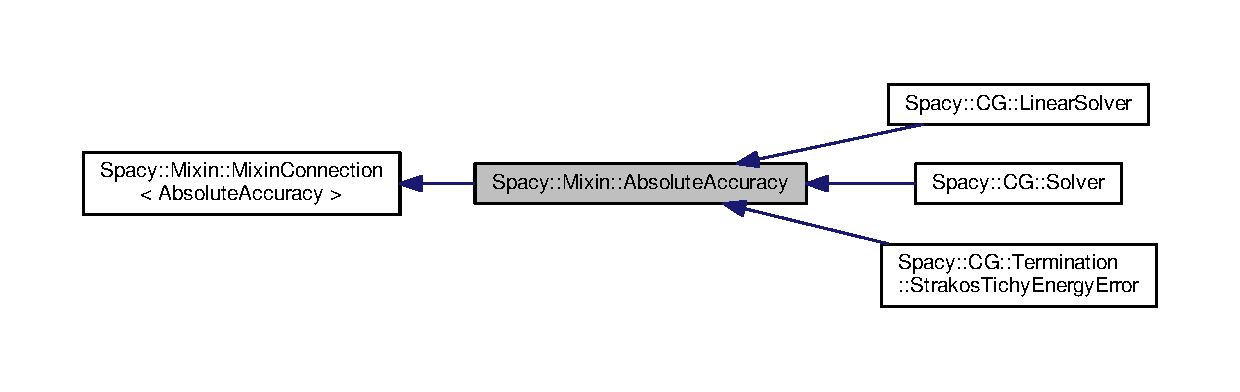
\includegraphics[width=350pt]{classSpacy_1_1Mixin_1_1AbsoluteAccuracy__inherit__graph}
\end{center}
\end{figure}


Collaboration diagram for Spacy\+:\+:Mixin\+:\+:Absolute\+Accuracy\+:\nopagebreak
\begin{figure}[H]
\begin{center}
\leavevmode
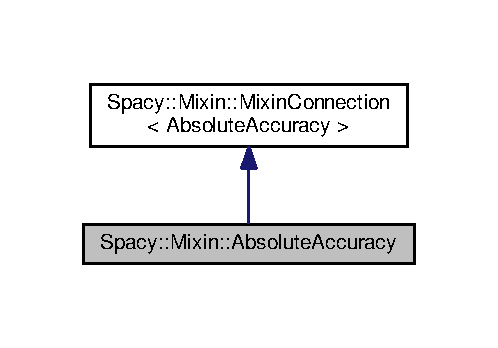
\includegraphics[width=239pt]{classSpacy_1_1Mixin_1_1AbsoluteAccuracy__coll__graph}
\end{center}
\end{figure}
\subsection*{Public Member Functions}
\begin{DoxyCompactItemize}
\item 
\hyperlink{classSpacy_1_1Mixin_1_1AbsoluteAccuracy_a98b58fa749e9b5363eb23a94011e7a67_a98b58fa749e9b5363eb23a94011e7a67}{Absolute\+Accuracy} (double accuracy=1e-\/15) noexcept
\begin{DoxyCompactList}\small\item\em Constructor. \end{DoxyCompactList}\item 
void \hyperlink{classSpacy_1_1Mixin_1_1AbsoluteAccuracy_a71cfcdc0c504be63c18c3e78df157738_a71cfcdc0c504be63c18c3e78df157738}{set\+Absolute\+Accuracy} (double accuracy)
\begin{DoxyCompactList}\small\item\em Set absolute accuracy. \end{DoxyCompactList}\item 
\hypertarget{classSpacy_1_1Mixin_1_1AbsoluteAccuracy_ad099a4a0a770133b56acaaf8783d4ba6}{}void {\bfseries set\+Absolute\+Accuracy} (\hyperlink{classSpacy_1_1Real}{Real} accuracy)\label{classSpacy_1_1Mixin_1_1AbsoluteAccuracy_ad099a4a0a770133b56acaaf8783d4ba6}

\item 
double \hyperlink{classSpacy_1_1Mixin_1_1AbsoluteAccuracy_aaa1fbd611cf85a098b71c22986778d8a_aaa1fbd611cf85a098b71c22986778d8a}{absolute\+Accuracy} () const noexcept
\begin{DoxyCompactList}\small\item\em Access absolute accuracy. \end{DoxyCompactList}\item 
void \hyperlink{classSpacy_1_1Mixin_1_1AbsoluteAccuracy_a05e2d07ee0ea883abf84a8c77e951cd8_a05e2d07ee0ea883abf84a8c77e951cd8}{attach\+Absolute\+Accuracy} (\hyperlink{classSpacy_1_1Mixin_1_1AbsoluteAccuracy}{Absolute\+Accuracy} \&other)
\begin{DoxyCompactList}\small\item\em Attach \hyperlink{classSpacy_1_1Mixin_1_1AbsoluteAccuracy}{Absolute\+Accuracy}. \end{DoxyCompactList}\item 
\hypertarget{classSpacy_1_1Mixin_1_1AbsoluteAccuracy_a8520fbc86f1b8a4dd1536683e925be1c}{}void \hyperlink{classSpacy_1_1Mixin_1_1AbsoluteAccuracy_a8520fbc86f1b8a4dd1536683e925be1c}{detach\+Absolute\+Accuracy} (\hyperlink{classSpacy_1_1Mixin_1_1AbsoluteAccuracy}{Absolute\+Accuracy} \&other)\label{classSpacy_1_1Mixin_1_1AbsoluteAccuracy_a8520fbc86f1b8a4dd1536683e925be1c}

\begin{DoxyCompactList}\small\item\em Detach verbosity before it gets deleted. \end{DoxyCompactList}\item 
\hypertarget{classSpacy_1_1Mixin_1_1AbsoluteAccuracy_a7e5910ba9a6ac7a4b332efdbbff27787}{}void \hyperlink{classSpacy_1_1Mixin_1_1AbsoluteAccuracy_a7e5910ba9a6ac7a4b332efdbbff27787}{update} (\hyperlink{classSpacy_1_1Mixin_1_1AbsoluteAccuracy}{Absolute\+Accuracy} $\ast$changed\+Subject)\label{classSpacy_1_1Mixin_1_1AbsoluteAccuracy_a7e5910ba9a6ac7a4b332efdbbff27787}

\begin{DoxyCompactList}\small\item\em update function for observer pattern. \end{DoxyCompactList}\end{DoxyCompactItemize}
\subsection*{Protected Member Functions}
\begin{DoxyCompactItemize}
\item 
\hypertarget{classSpacy_1_1Mixin_1_1MixinConnection_abb5520ee6b22dd993d78f142939a1ed4}{}void \hyperlink{classSpacy_1_1Mixin_1_1MixinConnection_abb5520ee6b22dd993d78f142939a1ed4}{attach} (\hyperlink{classSpacy_1_1Mixin_1_1AbsoluteAccuracy}{Absolute\+Accuracy} \&observer)\label{classSpacy_1_1Mixin_1_1MixinConnection_abb5520ee6b22dd993d78f142939a1ed4}

\begin{DoxyCompactList}\small\item\em Attach observer. \end{DoxyCompactList}\item 
\hypertarget{classSpacy_1_1Mixin_1_1MixinConnection_adda739590c487679c26f60e50aedb73f}{}void \hyperlink{classSpacy_1_1Mixin_1_1MixinConnection_adda739590c487679c26f60e50aedb73f}{detach} (\hyperlink{classSpacy_1_1Mixin_1_1AbsoluteAccuracy}{Absolute\+Accuracy} \&observer)\label{classSpacy_1_1Mixin_1_1MixinConnection_adda739590c487679c26f60e50aedb73f}

\begin{DoxyCompactList}\small\item\em Detach observer. \end{DoxyCompactList}\item 
\hypertarget{classSpacy_1_1Mixin_1_1MixinConnection_a1ddeaa78a3bb4a38c2cca36d1f99fe36}{}void \hyperlink{classSpacy_1_1Mixin_1_1MixinConnection_a1ddeaa78a3bb4a38c2cca36d1f99fe36}{notify} ()\label{classSpacy_1_1Mixin_1_1MixinConnection_a1ddeaa78a3bb4a38c2cca36d1f99fe36}

\begin{DoxyCompactList}\small\item\em Notify observers about changes. \end{DoxyCompactList}\end{DoxyCompactItemize}


\subsection{Detailed Description}
Mixin class for absolute accuracy. 

\subsection{Constructor \& Destructor Documentation}
\hypertarget{classSpacy_1_1Mixin_1_1AbsoluteAccuracy_a98b58fa749e9b5363eb23a94011e7a67_a98b58fa749e9b5363eb23a94011e7a67}{}\index{Spacy\+::\+Mixin\+::\+Absolute\+Accuracy@{Spacy\+::\+Mixin\+::\+Absolute\+Accuracy}!Absolute\+Accuracy@{Absolute\+Accuracy}}
\index{Absolute\+Accuracy@{Absolute\+Accuracy}!Spacy\+::\+Mixin\+::\+Absolute\+Accuracy@{Spacy\+::\+Mixin\+::\+Absolute\+Accuracy}}
\subsubsection[{Absolute\+Accuracy}]{\setlength{\rightskip}{0pt plus 5cm}Spacy\+::\+Mixin\+::\+Absolute\+Accuracy\+::\+Absolute\+Accuracy (
\begin{DoxyParamCaption}
\item[{double}]{accuracy = {\ttfamily 1e-\/15}}
\end{DoxyParamCaption}
)\hspace{0.3cm}{\ttfamily [explicit]}, {\ttfamily [noexcept]}}\label{classSpacy_1_1Mixin_1_1AbsoluteAccuracy_a98b58fa749e9b5363eb23a94011e7a67_a98b58fa749e9b5363eb23a94011e7a67}


Constructor. 


\begin{DoxyParams}{Parameters}
{\em accuracy} & absolute accuracy \\
\hline
\end{DoxyParams}


\subsection{Member Function Documentation}
\hypertarget{classSpacy_1_1Mixin_1_1AbsoluteAccuracy_aaa1fbd611cf85a098b71c22986778d8a_aaa1fbd611cf85a098b71c22986778d8a}{}\index{Spacy\+::\+Mixin\+::\+Absolute\+Accuracy@{Spacy\+::\+Mixin\+::\+Absolute\+Accuracy}!absolute\+Accuracy@{absolute\+Accuracy}}
\index{absolute\+Accuracy@{absolute\+Accuracy}!Spacy\+::\+Mixin\+::\+Absolute\+Accuracy@{Spacy\+::\+Mixin\+::\+Absolute\+Accuracy}}
\subsubsection[{absolute\+Accuracy}]{\setlength{\rightskip}{0pt plus 5cm}double Spacy\+::\+Mixin\+::\+Absolute\+Accuracy\+::absolute\+Accuracy (
\begin{DoxyParamCaption}
{}
\end{DoxyParamCaption}
) const\hspace{0.3cm}{\ttfamily [noexcept]}}\label{classSpacy_1_1Mixin_1_1AbsoluteAccuracy_aaa1fbd611cf85a098b71c22986778d8a_aaa1fbd611cf85a098b71c22986778d8a}


Access absolute accuracy. 

\begin{DoxyReturn}{Returns}
absolute accuracy 
\end{DoxyReturn}
\hypertarget{classSpacy_1_1Mixin_1_1AbsoluteAccuracy_a05e2d07ee0ea883abf84a8c77e951cd8_a05e2d07ee0ea883abf84a8c77e951cd8}{}\index{Spacy\+::\+Mixin\+::\+Absolute\+Accuracy@{Spacy\+::\+Mixin\+::\+Absolute\+Accuracy}!attach\+Absolute\+Accuracy@{attach\+Absolute\+Accuracy}}
\index{attach\+Absolute\+Accuracy@{attach\+Absolute\+Accuracy}!Spacy\+::\+Mixin\+::\+Absolute\+Accuracy@{Spacy\+::\+Mixin\+::\+Absolute\+Accuracy}}
\subsubsection[{attach\+Absolute\+Accuracy}]{\setlength{\rightskip}{0pt plus 5cm}void Spacy\+::\+Mixin\+::\+Absolute\+Accuracy\+::attach\+Absolute\+Accuracy (
\begin{DoxyParamCaption}
\item[{{\bf Absolute\+Accuracy} \&}]{other}
\end{DoxyParamCaption}
)}\label{classSpacy_1_1Mixin_1_1AbsoluteAccuracy_a05e2d07ee0ea883abf84a8c77e951cd8_a05e2d07ee0ea883abf84a8c77e951cd8}


Attach \hyperlink{classSpacy_1_1Mixin_1_1AbsoluteAccuracy}{Absolute\+Accuracy}. 

When \hyperlink{classSpacy_1_1Mixin_1_1AbsoluteAccuracy_a71cfcdc0c504be63c18c3e78df157738_a71cfcdc0c504be63c18c3e78df157738}{set\+Absolute\+Accuracy(double accuracy)} is called, then also other.\+set\+Absolute\+Accuracy(accuracy) is invoked. \hypertarget{classSpacy_1_1Mixin_1_1AbsoluteAccuracy_a71cfcdc0c504be63c18c3e78df157738_a71cfcdc0c504be63c18c3e78df157738}{}\index{Spacy\+::\+Mixin\+::\+Absolute\+Accuracy@{Spacy\+::\+Mixin\+::\+Absolute\+Accuracy}!set\+Absolute\+Accuracy@{set\+Absolute\+Accuracy}}
\index{set\+Absolute\+Accuracy@{set\+Absolute\+Accuracy}!Spacy\+::\+Mixin\+::\+Absolute\+Accuracy@{Spacy\+::\+Mixin\+::\+Absolute\+Accuracy}}
\subsubsection[{set\+Absolute\+Accuracy}]{\setlength{\rightskip}{0pt plus 5cm}void Spacy\+::\+Mixin\+::\+Absolute\+Accuracy\+::set\+Absolute\+Accuracy (
\begin{DoxyParamCaption}
\item[{double}]{accuracy}
\end{DoxyParamCaption}
)}\label{classSpacy_1_1Mixin_1_1AbsoluteAccuracy_a71cfcdc0c504be63c18c3e78df157738_a71cfcdc0c504be63c18c3e78df157738}


Set absolute accuracy. 


\begin{DoxyParams}{Parameters}
{\em accuracy} & absolute accuracy \\
\hline
\end{DoxyParams}


The documentation for this class was generated from the following file\+:\begin{DoxyCompactItemize}
\item 
Spacy/\+Util/\+Mixins/absolute\+Accuracy.\+hh\end{DoxyCompactItemize}

\hypertarget{classSpacy_1_1Mixin_1_1AdjointIndex}{}\section{Spacy\+:\+:Mixin\+:\+:Adjoint\+Index Class Reference}
\label{classSpacy_1_1Mixin_1_1AdjointIndex}\index{Spacy\+::\+Mixin\+::\+Adjoint\+Index@{Spacy\+::\+Mixin\+::\+Adjoint\+Index}}


Mixin class for index of the adjoint variable.  




{\ttfamily \#include $<$adjoint\+Index.\+hh$>$}



Inheritance diagram for Spacy\+:\+:Mixin\+:\+:Adjoint\+Index\+:\nopagebreak
\begin{figure}[H]
\begin{center}
\leavevmode
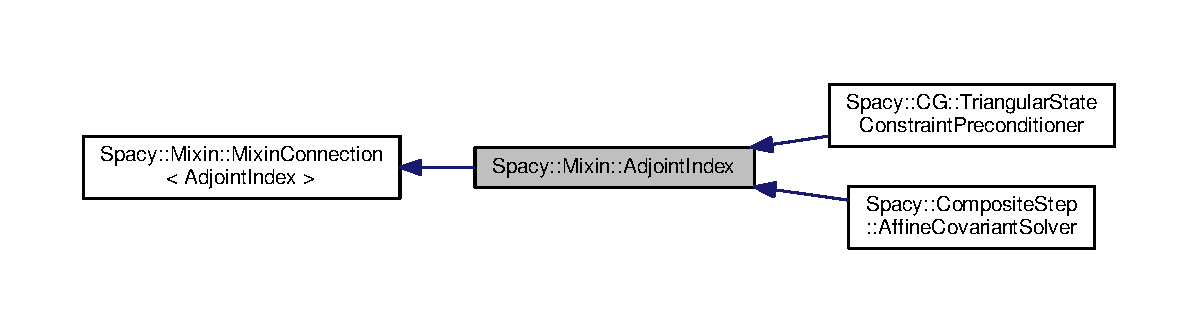
\includegraphics[width=350pt]{classSpacy_1_1Mixin_1_1AdjointIndex__inherit__graph}
\end{center}
\end{figure}


Collaboration diagram for Spacy\+:\+:Mixin\+:\+:Adjoint\+Index\+:\nopagebreak
\begin{figure}[H]
\begin{center}
\leavevmode
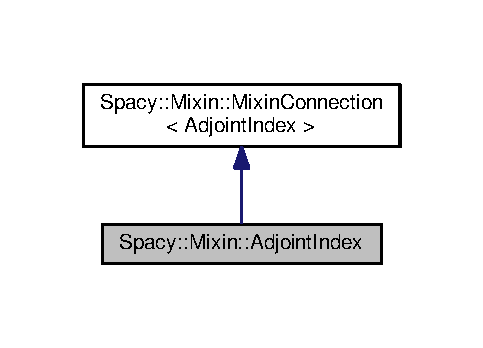
\includegraphics[width=232pt]{classSpacy_1_1Mixin_1_1AdjointIndex__coll__graph}
\end{center}
\end{figure}
\subsection*{Public Member Functions}
\begin{DoxyCompactItemize}
\item 
\hyperlink{classSpacy_1_1Mixin_1_1AdjointIndex_a18dca16025bfc2af67da2eee34be9699_a18dca16025bfc2af67da2eee34be9699}{Adjoint\+Index} (unsigned index=2) noexcept
\begin{DoxyCompactList}\small\item\em Constructor. \end{DoxyCompactList}\item 
void \hyperlink{classSpacy_1_1Mixin_1_1AdjointIndex_a30d4dd8b61175144c84c5bbf964528d7_a30d4dd8b61175144c84c5bbf964528d7}{set\+Adjoint\+Index} (unsigned index)
\begin{DoxyCompactList}\small\item\em Set index of the adjoint variable. \end{DoxyCompactList}\item 
double \hyperlink{classSpacy_1_1Mixin_1_1AdjointIndex_afd5c0f6bd67d20c88ea65b7f8fe4ab45_afd5c0f6bd67d20c88ea65b7f8fe4ab45}{adjoint\+Index} () const noexcept
\begin{DoxyCompactList}\small\item\em Access index of the adjoint variable. \end{DoxyCompactList}\item 
void \hyperlink{classSpacy_1_1Mixin_1_1AdjointIndex_a6ac8bb62f7d40cdf7aee68539026a647_a6ac8bb62f7d40cdf7aee68539026a647}{attach\+Adjoint\+Index} (\hyperlink{classSpacy_1_1Mixin_1_1AdjointIndex}{Adjoint\+Index} \&other)
\begin{DoxyCompactList}\small\item\em Attach adjoint index. \end{DoxyCompactList}\item 
\hypertarget{classSpacy_1_1Mixin_1_1AdjointIndex_af07504e2900cd83446469b4bb0ce0a4a}{}void \hyperlink{classSpacy_1_1Mixin_1_1AdjointIndex_af07504e2900cd83446469b4bb0ce0a4a}{detach\+Adjoint\+Index} (\hyperlink{classSpacy_1_1Mixin_1_1AdjointIndex}{Adjoint\+Index} \&other)\label{classSpacy_1_1Mixin_1_1AdjointIndex_af07504e2900cd83446469b4bb0ce0a4a}

\begin{DoxyCompactList}\small\item\em Detach verbosity before it gets deleted. \end{DoxyCompactList}\item 
\hypertarget{classSpacy_1_1Mixin_1_1AdjointIndex_ad91ccf68601950801cd062afee8a8cf2}{}void \hyperlink{classSpacy_1_1Mixin_1_1AdjointIndex_ad91ccf68601950801cd062afee8a8cf2}{update} (\hyperlink{classSpacy_1_1Mixin_1_1AdjointIndex}{Adjoint\+Index} $\ast$changed\+Subject)\label{classSpacy_1_1Mixin_1_1AdjointIndex_ad91ccf68601950801cd062afee8a8cf2}

\begin{DoxyCompactList}\small\item\em update function for observer pattern. \end{DoxyCompactList}\end{DoxyCompactItemize}
\subsection*{Protected Member Functions}
\begin{DoxyCompactItemize}
\item 
\hypertarget{classSpacy_1_1Mixin_1_1MixinConnection_abb5520ee6b22dd993d78f142939a1ed4}{}void \hyperlink{classSpacy_1_1Mixin_1_1MixinConnection_abb5520ee6b22dd993d78f142939a1ed4}{attach} (\hyperlink{classSpacy_1_1Mixin_1_1AdjointIndex}{Adjoint\+Index} \&observer)\label{classSpacy_1_1Mixin_1_1MixinConnection_abb5520ee6b22dd993d78f142939a1ed4}

\begin{DoxyCompactList}\small\item\em Attach observer. \end{DoxyCompactList}\item 
\hypertarget{classSpacy_1_1Mixin_1_1MixinConnection_adda739590c487679c26f60e50aedb73f}{}void \hyperlink{classSpacy_1_1Mixin_1_1MixinConnection_adda739590c487679c26f60e50aedb73f}{detach} (\hyperlink{classSpacy_1_1Mixin_1_1AdjointIndex}{Adjoint\+Index} \&observer)\label{classSpacy_1_1Mixin_1_1MixinConnection_adda739590c487679c26f60e50aedb73f}

\begin{DoxyCompactList}\small\item\em Detach observer. \end{DoxyCompactList}\item 
\hypertarget{classSpacy_1_1Mixin_1_1MixinConnection_a1ddeaa78a3bb4a38c2cca36d1f99fe36}{}void \hyperlink{classSpacy_1_1Mixin_1_1MixinConnection_a1ddeaa78a3bb4a38c2cca36d1f99fe36}{notify} ()\label{classSpacy_1_1Mixin_1_1MixinConnection_a1ddeaa78a3bb4a38c2cca36d1f99fe36}

\begin{DoxyCompactList}\small\item\em Notify observers about changes. \end{DoxyCompactList}\end{DoxyCompactItemize}


\subsection{Detailed Description}
Mixin class for index of the adjoint variable. 

\subsection{Constructor \& Destructor Documentation}
\hypertarget{classSpacy_1_1Mixin_1_1AdjointIndex_a18dca16025bfc2af67da2eee34be9699_a18dca16025bfc2af67da2eee34be9699}{}\index{Spacy\+::\+Mixin\+::\+Adjoint\+Index@{Spacy\+::\+Mixin\+::\+Adjoint\+Index}!Adjoint\+Index@{Adjoint\+Index}}
\index{Adjoint\+Index@{Adjoint\+Index}!Spacy\+::\+Mixin\+::\+Adjoint\+Index@{Spacy\+::\+Mixin\+::\+Adjoint\+Index}}
\subsubsection[{Adjoint\+Index}]{\setlength{\rightskip}{0pt plus 5cm}Spacy\+::\+Mixin\+::\+Adjoint\+Index\+::\+Adjoint\+Index (
\begin{DoxyParamCaption}
\item[{unsigned}]{index = {\ttfamily 2}}
\end{DoxyParamCaption}
)\hspace{0.3cm}{\ttfamily [explicit]}, {\ttfamily [noexcept]}}\label{classSpacy_1_1Mixin_1_1AdjointIndex_a18dca16025bfc2af67da2eee34be9699_a18dca16025bfc2af67da2eee34be9699}


Constructor. 


\begin{DoxyParams}{Parameters}
{\em index} & index of the adjoint variable. \\
\hline
\end{DoxyParams}


\subsection{Member Function Documentation}
\hypertarget{classSpacy_1_1Mixin_1_1AdjointIndex_afd5c0f6bd67d20c88ea65b7f8fe4ab45_afd5c0f6bd67d20c88ea65b7f8fe4ab45}{}\index{Spacy\+::\+Mixin\+::\+Adjoint\+Index@{Spacy\+::\+Mixin\+::\+Adjoint\+Index}!adjoint\+Index@{adjoint\+Index}}
\index{adjoint\+Index@{adjoint\+Index}!Spacy\+::\+Mixin\+::\+Adjoint\+Index@{Spacy\+::\+Mixin\+::\+Adjoint\+Index}}
\subsubsection[{adjoint\+Index}]{\setlength{\rightskip}{0pt plus 5cm}double Spacy\+::\+Mixin\+::\+Adjoint\+Index\+::adjoint\+Index (
\begin{DoxyParamCaption}
{}
\end{DoxyParamCaption}
) const\hspace{0.3cm}{\ttfamily [noexcept]}}\label{classSpacy_1_1Mixin_1_1AdjointIndex_afd5c0f6bd67d20c88ea65b7f8fe4ab45_afd5c0f6bd67d20c88ea65b7f8fe4ab45}


Access index of the adjoint variable. 

\begin{DoxyReturn}{Returns}
index of the adjoint variable 
\end{DoxyReturn}
\hypertarget{classSpacy_1_1Mixin_1_1AdjointIndex_a6ac8bb62f7d40cdf7aee68539026a647_a6ac8bb62f7d40cdf7aee68539026a647}{}\index{Spacy\+::\+Mixin\+::\+Adjoint\+Index@{Spacy\+::\+Mixin\+::\+Adjoint\+Index}!attach\+Adjoint\+Index@{attach\+Adjoint\+Index}}
\index{attach\+Adjoint\+Index@{attach\+Adjoint\+Index}!Spacy\+::\+Mixin\+::\+Adjoint\+Index@{Spacy\+::\+Mixin\+::\+Adjoint\+Index}}
\subsubsection[{attach\+Adjoint\+Index}]{\setlength{\rightskip}{0pt plus 5cm}void Spacy\+::\+Mixin\+::\+Adjoint\+Index\+::attach\+Adjoint\+Index (
\begin{DoxyParamCaption}
\item[{{\bf Adjoint\+Index} \&}]{other}
\end{DoxyParamCaption}
)}\label{classSpacy_1_1Mixin_1_1AdjointIndex_a6ac8bb62f7d40cdf7aee68539026a647_a6ac8bb62f7d40cdf7aee68539026a647}


Attach adjoint index. 

When \hyperlink{classSpacy_1_1Mixin_1_1AdjointIndex_a30d4dd8b61175144c84c5bbf964528d7_a30d4dd8b61175144c84c5bbf964528d7}{set\+Adjoint\+Index(unsigned index)} is called, then also other.\+set\+Adjoint\+Index(unsigned index) is invoked. \hypertarget{classSpacy_1_1Mixin_1_1AdjointIndex_a30d4dd8b61175144c84c5bbf964528d7_a30d4dd8b61175144c84c5bbf964528d7}{}\index{Spacy\+::\+Mixin\+::\+Adjoint\+Index@{Spacy\+::\+Mixin\+::\+Adjoint\+Index}!set\+Adjoint\+Index@{set\+Adjoint\+Index}}
\index{set\+Adjoint\+Index@{set\+Adjoint\+Index}!Spacy\+::\+Mixin\+::\+Adjoint\+Index@{Spacy\+::\+Mixin\+::\+Adjoint\+Index}}
\subsubsection[{set\+Adjoint\+Index}]{\setlength{\rightskip}{0pt plus 5cm}void Spacy\+::\+Mixin\+::\+Adjoint\+Index\+::set\+Adjoint\+Index (
\begin{DoxyParamCaption}
\item[{unsigned}]{index}
\end{DoxyParamCaption}
)}\label{classSpacy_1_1Mixin_1_1AdjointIndex_a30d4dd8b61175144c84c5bbf964528d7_a30d4dd8b61175144c84c5bbf964528d7}


Set index of the adjoint variable. 


\begin{DoxyParams}{Parameters}
{\em index} & new index of the adjoint variable \\
\hline
\end{DoxyParams}


The documentation for this class was generated from the following file\+:\begin{DoxyCompactItemize}
\item 
Spacy/\+Util/\+Mixins/adjoint\+Index.\+hh\end{DoxyCompactItemize}

\hypertarget{classSpacy_1_1Newton_1_1Termination_1_1AffineContravariant}{}\section{Spacy\+:\+:Newton\+:\+:Termination\+:\+:Affine\+Contravariant Class Reference}
\label{classSpacy_1_1Newton_1_1Termination_1_1AffineContravariant}\index{Spacy\+::\+Newton\+::\+Termination\+::\+Affine\+Contravariant@{Spacy\+::\+Newton\+::\+Termination\+::\+Affine\+Contravariant}}


Affine contravariant relative error criterion.  




{\ttfamily \#include $<$termination\+Criteria.\+hh$>$}



Inheritance diagram for Spacy\+:\+:Newton\+:\+:Termination\+:\+:Affine\+Contravariant\+:\nopagebreak
\begin{figure}[H]
\begin{center}
\leavevmode
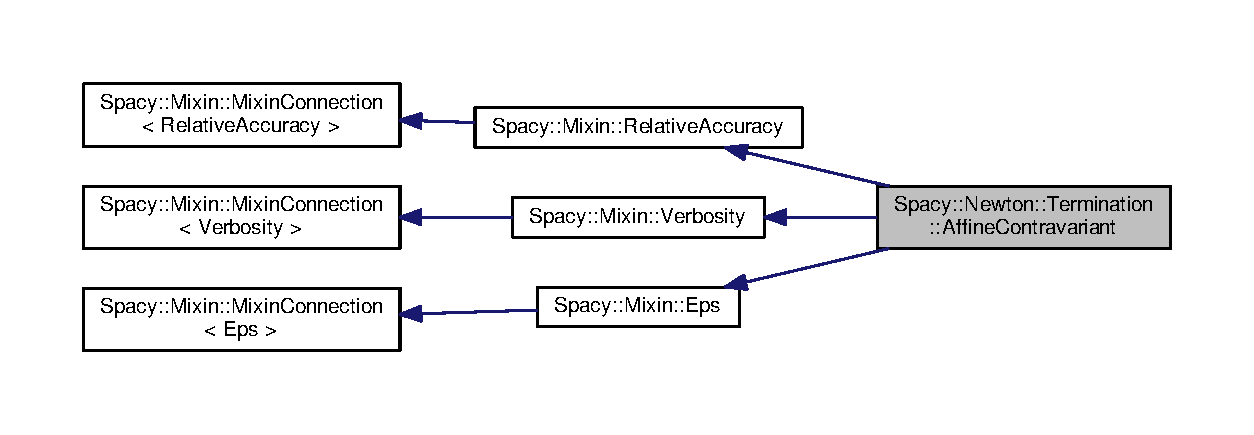
\includegraphics[width=350pt]{classSpacy_1_1Newton_1_1Termination_1_1AffineContravariant__inherit__graph}
\end{center}
\end{figure}


Collaboration diagram for Spacy\+:\+:Newton\+:\+:Termination\+:\+:Affine\+Contravariant\+:\nopagebreak
\begin{figure}[H]
\begin{center}
\leavevmode
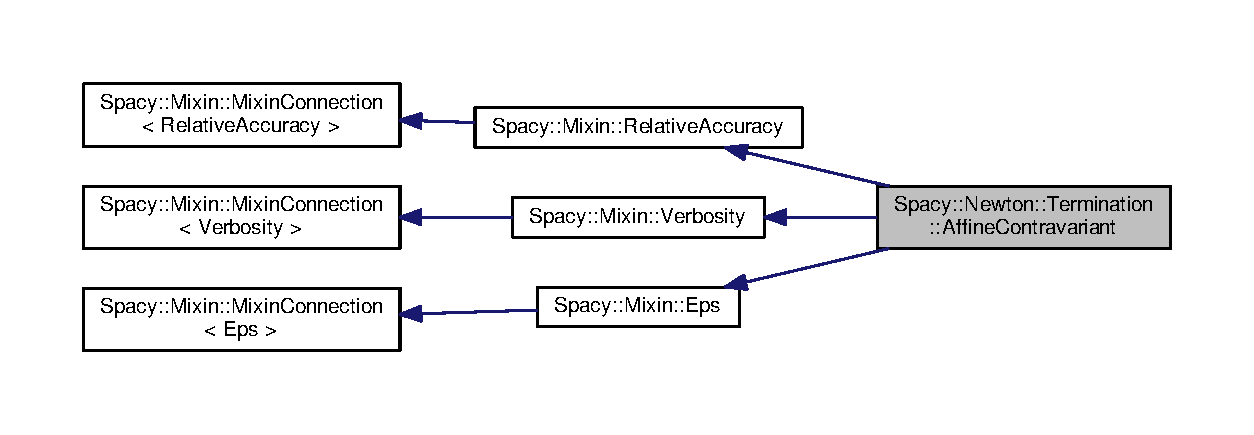
\includegraphics[width=350pt]{classSpacy_1_1Newton_1_1Termination_1_1AffineContravariant__coll__graph}
\end{center}
\end{figure}
\subsection*{Public Member Functions}
\begin{DoxyCompactItemize}
\item 
\hypertarget{classSpacy_1_1Newton_1_1Termination_1_1AffineContravariant_a1ded6963049723d42c8917e39b77194d}{}\hyperlink{classSpacy_1_1Newton_1_1Termination_1_1AffineContravariant_a1ded6963049723d42c8917e39b77194d}{Affine\+Contravariant} (const \hyperlink{group__SpacyGroup_ga3f89622eba80cf840b2a7102f1303455_ga3f89622eba80cf840b2a7102f1303455}{Operator} \&F, double \hyperlink{classSpacy_1_1Mixin_1_1RelativeAccuracy_a1da618cf9265c2edae354524df4a7f8a_a1da618cf9265c2edae354524df4a7f8a}{relative\+Accuracy}, bool \hyperlink{classSpacy_1_1Mixin_1_1Verbosity_ad367a7328578546938fd2a7e52ab3793_ad367a7328578546938fd2a7e52ab3793}{verbose}=false)\label{classSpacy_1_1Newton_1_1Termination_1_1AffineContravariant_a1ded6963049723d42c8917e39b77194d}

\begin{DoxyCompactList}\small\item\em Constructor. \end{DoxyCompactList}\item 
bool \hyperlink{classSpacy_1_1Newton_1_1Termination_1_1AffineContravariant_a16b9829fd882e948b5d273b80c549f4b_a16b9829fd882e948b5d273b80c549f4b}{operator()} (\hyperlink{classSpacy_1_1DampingFactor}{Damping\+Factor} nu, const \hyperlink{classSpacy_1_1Vector}{Vector} \&x, const \hyperlink{classSpacy_1_1Vector}{Vector} \&) const 
\begin{DoxyCompactList}\small\item\em Apply termination criterion. \end{DoxyCompactList}\item 
void \hyperlink{classSpacy_1_1Mixin_1_1RelativeAccuracy_aee88b71e80aca446a179f1310408a1e3_aee88b71e80aca446a179f1310408a1e3}{set\+Relative\+Accuracy} (double accuracy)
\begin{DoxyCompactList}\small\item\em Set relative accuracy. \end{DoxyCompactList}\item 
double \hyperlink{classSpacy_1_1Mixin_1_1RelativeAccuracy_a1da618cf9265c2edae354524df4a7f8a_a1da618cf9265c2edae354524df4a7f8a}{relative\+Accuracy} () const noexcept
\begin{DoxyCompactList}\small\item\em Access relative accuracy. \end{DoxyCompactList}\item 
void \hyperlink{classSpacy_1_1Mixin_1_1RelativeAccuracy_ae299bb5419df551cc93c6397e5b1b58b_ae299bb5419df551cc93c6397e5b1b58b}{attach\+Relative\+Accuracy} (\hyperlink{classSpacy_1_1Mixin_1_1RelativeAccuracy_ad843319a8782b47291fa31334e8bbd2a_ad843319a8782b47291fa31334e8bbd2a}{Relative\+Accuracy} \&other)
\begin{DoxyCompactList}\small\item\em Attach \hyperlink{classSpacy_1_1Mixin_1_1RelativeAccuracy}{Relative\+Accuracy}. \end{DoxyCompactList}\item 
\hypertarget{classSpacy_1_1Mixin_1_1RelativeAccuracy_a2636cde30aab8415e19e25fc12489e57}{}void \hyperlink{classSpacy_1_1Mixin_1_1RelativeAccuracy_a2636cde30aab8415e19e25fc12489e57}{detach\+Relative\+Accuracy} (\hyperlink{classSpacy_1_1Mixin_1_1RelativeAccuracy_ad843319a8782b47291fa31334e8bbd2a_ad843319a8782b47291fa31334e8bbd2a}{Relative\+Accuracy} \&other)\label{classSpacy_1_1Mixin_1_1RelativeAccuracy_a2636cde30aab8415e19e25fc12489e57}

\begin{DoxyCompactList}\small\item\em Detach \hyperlink{classSpacy_1_1Mixin_1_1RelativeAccuracy}{Relative\+Accuracy} before it gets deleted. \end{DoxyCompactList}\item 
\hypertarget{classSpacy_1_1Mixin_1_1RelativeAccuracy_acf0b58224d9a2879d05b5d2947f37527}{}void \hyperlink{classSpacy_1_1Mixin_1_1RelativeAccuracy_acf0b58224d9a2879d05b5d2947f37527}{update} (\hyperlink{classSpacy_1_1Mixin_1_1RelativeAccuracy_ad843319a8782b47291fa31334e8bbd2a_ad843319a8782b47291fa31334e8bbd2a}{Relative\+Accuracy} $\ast$changed\+Subject)\label{classSpacy_1_1Mixin_1_1RelativeAccuracy_acf0b58224d9a2879d05b5d2947f37527}

\begin{DoxyCompactList}\small\item\em update function for observer pattern. \end{DoxyCompactList}\item 
void \hyperlink{classSpacy_1_1Mixin_1_1Verbosity_a0365d293ab27e27da9496c668020aefb_a0365d293ab27e27da9496c668020aefb}{set\+Verbosity} (bool \hyperlink{classSpacy_1_1Mixin_1_1Verbosity_ad367a7328578546938fd2a7e52ab3793_ad367a7328578546938fd2a7e52ab3793}{verbose})
\begin{DoxyCompactList}\small\item\em Enable/disable verbosity. \end{DoxyCompactList}\item 
bool \hyperlink{classSpacy_1_1Mixin_1_1Verbosity_ad367a7328578546938fd2a7e52ab3793_ad367a7328578546938fd2a7e52ab3793}{verbose} () const noexcept
\begin{DoxyCompactList}\small\item\em Check if verbosity is turned on. \end{DoxyCompactList}\item 
void \hyperlink{classSpacy_1_1Mixin_1_1Verbosity_af84a4b3c933f252a5840ab63d4a38325_af84a4b3c933f252a5840ab63d4a38325}{set\+Verbosity\+Level} (unsigned level) noexcept
\begin{DoxyCompactList}\small\item\em Set verbosity level. \end{DoxyCompactList}\item 
unsigned \hyperlink{classSpacy_1_1Mixin_1_1Verbosity_a2131f495d276c95d2d6534a6dfce6f9f_a2131f495d276c95d2d6534a6dfce6f9f}{verbosity\+Level} () const noexcept
\begin{DoxyCompactList}\small\item\em Access verbosity level. \end{DoxyCompactList}\item 
void \hyperlink{classSpacy_1_1Mixin_1_1Verbosity_a69fe3a0107ec34780f1d74b46b1b53b5_a69fe3a0107ec34780f1d74b46b1b53b5}{attach\+Verbosity} (\hyperlink{classSpacy_1_1Mixin_1_1Verbosity_aefe2f237b0456c4bced001fbfa75f92e_aefe2f237b0456c4bced001fbfa75f92e}{Verbosity} \&other)
\begin{DoxyCompactList}\small\item\em Attach verbosity. \end{DoxyCompactList}\item 
\hypertarget{classSpacy_1_1Mixin_1_1Verbosity_a86ec8efe73d1ce2768bf645f0627b325}{}void \hyperlink{classSpacy_1_1Mixin_1_1Verbosity_a86ec8efe73d1ce2768bf645f0627b325}{detach\+Verbosity} (\hyperlink{classSpacy_1_1Mixin_1_1Verbosity_aefe2f237b0456c4bced001fbfa75f92e_aefe2f237b0456c4bced001fbfa75f92e}{Verbosity} \&other)\label{classSpacy_1_1Mixin_1_1Verbosity_a86ec8efe73d1ce2768bf645f0627b325}

\begin{DoxyCompactList}\small\item\em Detach verbosity before it gets deleted. \end{DoxyCompactList}\item 
\hypertarget{classSpacy_1_1Mixin_1_1Verbosity_a8cff860c587fcda2cdc86ba744302b33}{}void \hyperlink{classSpacy_1_1Mixin_1_1Verbosity_a8cff860c587fcda2cdc86ba744302b33}{update} (\hyperlink{classSpacy_1_1Mixin_1_1Verbosity_aefe2f237b0456c4bced001fbfa75f92e_aefe2f237b0456c4bced001fbfa75f92e}{Verbosity} $\ast$changed\+Subject)\label{classSpacy_1_1Mixin_1_1Verbosity_a8cff860c587fcda2cdc86ba744302b33}

\begin{DoxyCompactList}\small\item\em update function for observer pattern. \end{DoxyCompactList}\item 
void \hyperlink{classSpacy_1_1Mixin_1_1Eps_a1bbfd62541610d5d80f2782ab77158e4_a1bbfd62541610d5d80f2782ab77158e4}{set\+Eps} (double \hyperlink{classSpacy_1_1Mixin_1_1Eps_a40e2ba8f3abd2b5370ef41238cfaaf8b_a40e2ba8f3abd2b5370ef41238cfaaf8b}{eps})
\begin{DoxyCompactList}\small\item\em Set maximal attainable accuracy $\varepsilon$. \end{DoxyCompactList}\item 
double \hyperlink{classSpacy_1_1Mixin_1_1Eps_a40e2ba8f3abd2b5370ef41238cfaaf8b_a40e2ba8f3abd2b5370ef41238cfaaf8b}{eps} () const noexcept
\begin{DoxyCompactList}\small\item\em Access maximal attainable accuracy. \end{DoxyCompactList}\item 
double \hyperlink{classSpacy_1_1Mixin_1_1Eps_a29e8c25dc3f1fdede57b8eb06f520fe1_a29e8c25dc3f1fdede57b8eb06f520fe1}{sqrt\+Eps} () const noexcept
\begin{DoxyCompactList}\small\item\em Access square root of maximal attainable accuracy. \end{DoxyCompactList}\item 
double \hyperlink{classSpacy_1_1Mixin_1_1Eps_a1879ebbf1b467cb4be36bcc63307018d_a1879ebbf1b467cb4be36bcc63307018d}{cbrt\+Eps} () const noexcept
\begin{DoxyCompactList}\small\item\em Get third root of maximal attainable accuracy. \end{DoxyCompactList}\item 
void \hyperlink{classSpacy_1_1Mixin_1_1Eps_af69cd3dee52e723302b21ca2a25f1192_af69cd3dee52e723302b21ca2a25f1192}{attach\+Eps} (\hyperlink{classSpacy_1_1Mixin_1_1Eps_a51dbe0b9cc950e0f3dfd34a481f08ae4_a51dbe0b9cc950e0f3dfd34a481f08ae4}{Eps} \&other)
\begin{DoxyCompactList}\small\item\em Attach \hyperlink{classSpacy_1_1Mixin_1_1Eps}{Eps}. \end{DoxyCompactList}\item 
\hypertarget{classSpacy_1_1Mixin_1_1Eps_ab49910e189cb86b6fd6f89b6f2af14cc}{}void \hyperlink{classSpacy_1_1Mixin_1_1Eps_ab49910e189cb86b6fd6f89b6f2af14cc}{detach\+Eps} (\hyperlink{classSpacy_1_1Mixin_1_1Eps_a51dbe0b9cc950e0f3dfd34a481f08ae4_a51dbe0b9cc950e0f3dfd34a481f08ae4}{Eps} \&other)\label{classSpacy_1_1Mixin_1_1Eps_ab49910e189cb86b6fd6f89b6f2af14cc}

\begin{DoxyCompactList}\small\item\em Detach \hyperlink{classSpacy_1_1Mixin_1_1Eps}{Eps} before it gets deleted. \end{DoxyCompactList}\item 
\hypertarget{classSpacy_1_1Mixin_1_1Eps_a151216968daef3da5f5cdc0b957ce01b}{}void \hyperlink{classSpacy_1_1Mixin_1_1Eps_a151216968daef3da5f5cdc0b957ce01b}{update} (\hyperlink{classSpacy_1_1Mixin_1_1Eps_a51dbe0b9cc950e0f3dfd34a481f08ae4_a51dbe0b9cc950e0f3dfd34a481f08ae4}{Eps} $\ast$changed\+Subject)\label{classSpacy_1_1Mixin_1_1Eps_a151216968daef3da5f5cdc0b957ce01b}

\begin{DoxyCompactList}\small\item\em update function for observer pattern. \end{DoxyCompactList}\end{DoxyCompactItemize}
\subsection*{Protected Member Functions}
\begin{DoxyCompactItemize}
\item 
\hypertarget{classSpacy_1_1Mixin_1_1MixinConnection_abb5520ee6b22dd993d78f142939a1ed4}{}void \hyperlink{classSpacy_1_1Mixin_1_1MixinConnection_abb5520ee6b22dd993d78f142939a1ed4}{attach} (\hyperlink{classSpacy_1_1Mixin_1_1RelativeAccuracy_ad843319a8782b47291fa31334e8bbd2a_ad843319a8782b47291fa31334e8bbd2a}{Relative\+Accuracy} \&observer)\label{classSpacy_1_1Mixin_1_1MixinConnection_abb5520ee6b22dd993d78f142939a1ed4}

\begin{DoxyCompactList}\small\item\em Attach observer. \end{DoxyCompactList}\item 
\hypertarget{classSpacy_1_1Mixin_1_1MixinConnection_adda739590c487679c26f60e50aedb73f}{}void \hyperlink{classSpacy_1_1Mixin_1_1MixinConnection_adda739590c487679c26f60e50aedb73f}{detach} (\hyperlink{classSpacy_1_1Mixin_1_1RelativeAccuracy_ad843319a8782b47291fa31334e8bbd2a_ad843319a8782b47291fa31334e8bbd2a}{Relative\+Accuracy} \&observer)\label{classSpacy_1_1Mixin_1_1MixinConnection_adda739590c487679c26f60e50aedb73f}

\begin{DoxyCompactList}\small\item\em Detach observer. \end{DoxyCompactList}\item 
\hypertarget{classSpacy_1_1Mixin_1_1MixinConnection_a1ddeaa78a3bb4a38c2cca36d1f99fe36}{}void \hyperlink{classSpacy_1_1Mixin_1_1MixinConnection_a1ddeaa78a3bb4a38c2cca36d1f99fe36}{notify} ()\label{classSpacy_1_1Mixin_1_1MixinConnection_a1ddeaa78a3bb4a38c2cca36d1f99fe36}

\begin{DoxyCompactList}\small\item\em Notify observers about changes. \end{DoxyCompactList}\item 
\hypertarget{classSpacy_1_1Mixin_1_1MixinConnection_abb5520ee6b22dd993d78f142939a1ed4}{}void \hyperlink{classSpacy_1_1Mixin_1_1MixinConnection_abb5520ee6b22dd993d78f142939a1ed4}{attach} (\hyperlink{classSpacy_1_1Mixin_1_1Verbosity_aefe2f237b0456c4bced001fbfa75f92e_aefe2f237b0456c4bced001fbfa75f92e}{Verbosity} \&observer)\label{classSpacy_1_1Mixin_1_1MixinConnection_abb5520ee6b22dd993d78f142939a1ed4}

\begin{DoxyCompactList}\small\item\em Attach observer. \end{DoxyCompactList}\item 
\hypertarget{classSpacy_1_1Mixin_1_1MixinConnection_adda739590c487679c26f60e50aedb73f}{}void \hyperlink{classSpacy_1_1Mixin_1_1MixinConnection_adda739590c487679c26f60e50aedb73f}{detach} (\hyperlink{classSpacy_1_1Mixin_1_1Verbosity_aefe2f237b0456c4bced001fbfa75f92e_aefe2f237b0456c4bced001fbfa75f92e}{Verbosity} \&observer)\label{classSpacy_1_1Mixin_1_1MixinConnection_adda739590c487679c26f60e50aedb73f}

\begin{DoxyCompactList}\small\item\em Detach observer. \end{DoxyCompactList}\item 
\hypertarget{classSpacy_1_1Mixin_1_1MixinConnection_a1ddeaa78a3bb4a38c2cca36d1f99fe36}{}void \hyperlink{classSpacy_1_1Mixin_1_1MixinConnection_a1ddeaa78a3bb4a38c2cca36d1f99fe36}{notify} ()\label{classSpacy_1_1Mixin_1_1MixinConnection_a1ddeaa78a3bb4a38c2cca36d1f99fe36}

\begin{DoxyCompactList}\small\item\em Notify observers about changes. \end{DoxyCompactList}\item 
\hypertarget{classSpacy_1_1Mixin_1_1MixinConnection_abb5520ee6b22dd993d78f142939a1ed4}{}void \hyperlink{classSpacy_1_1Mixin_1_1MixinConnection_abb5520ee6b22dd993d78f142939a1ed4}{attach} (\hyperlink{classSpacy_1_1Mixin_1_1Eps_a51dbe0b9cc950e0f3dfd34a481f08ae4_a51dbe0b9cc950e0f3dfd34a481f08ae4}{Eps} \&observer)\label{classSpacy_1_1Mixin_1_1MixinConnection_abb5520ee6b22dd993d78f142939a1ed4}

\begin{DoxyCompactList}\small\item\em Attach observer. \end{DoxyCompactList}\item 
\hypertarget{classSpacy_1_1Mixin_1_1MixinConnection_adda739590c487679c26f60e50aedb73f}{}void \hyperlink{classSpacy_1_1Mixin_1_1MixinConnection_adda739590c487679c26f60e50aedb73f}{detach} (\hyperlink{classSpacy_1_1Mixin_1_1Eps_a51dbe0b9cc950e0f3dfd34a481f08ae4_a51dbe0b9cc950e0f3dfd34a481f08ae4}{Eps} \&observer)\label{classSpacy_1_1Mixin_1_1MixinConnection_adda739590c487679c26f60e50aedb73f}

\begin{DoxyCompactList}\small\item\em Detach observer. \end{DoxyCompactList}\item 
\hypertarget{classSpacy_1_1Mixin_1_1MixinConnection_a1ddeaa78a3bb4a38c2cca36d1f99fe36}{}void \hyperlink{classSpacy_1_1Mixin_1_1MixinConnection_a1ddeaa78a3bb4a38c2cca36d1f99fe36}{notify} ()\label{classSpacy_1_1Mixin_1_1MixinConnection_a1ddeaa78a3bb4a38c2cca36d1f99fe36}

\begin{DoxyCompactList}\small\item\em Notify observers about changes. \end{DoxyCompactList}\end{DoxyCompactItemize}


\subsection{Detailed Description}
Affine contravariant relative error criterion. 

\subsection{Member Function Documentation}
\hypertarget{classSpacy_1_1Mixin_1_1Eps_af69cd3dee52e723302b21ca2a25f1192_af69cd3dee52e723302b21ca2a25f1192}{}\index{Spacy\+::\+Newton\+::\+Termination\+::\+Affine\+Contravariant@{Spacy\+::\+Newton\+::\+Termination\+::\+Affine\+Contravariant}!attach\+Eps@{attach\+Eps}}
\index{attach\+Eps@{attach\+Eps}!Spacy\+::\+Newton\+::\+Termination\+::\+Affine\+Contravariant@{Spacy\+::\+Newton\+::\+Termination\+::\+Affine\+Contravariant}}
\subsubsection[{attach\+Eps}]{\setlength{\rightskip}{0pt plus 5cm}void Spacy\+::\+Mixin\+::\+Eps\+::attach\+Eps (
\begin{DoxyParamCaption}
\item[{{\bf Eps} \&}]{other}
\end{DoxyParamCaption}
)\hspace{0.3cm}{\ttfamily [inherited]}}\label{classSpacy_1_1Mixin_1_1Eps_af69cd3dee52e723302b21ca2a25f1192_af69cd3dee52e723302b21ca2a25f1192}


Attach \hyperlink{classSpacy_1_1Mixin_1_1Eps}{Eps}. 

When \hyperlink{classSpacy_1_1Mixin_1_1Eps_a1bbfd62541610d5d80f2782ab77158e4_a1bbfd62541610d5d80f2782ab77158e4}{set\+Eps(double eps)} is called, then also other.\+set\+Eps(eps) is invoked. \hypertarget{classSpacy_1_1Mixin_1_1RelativeAccuracy_ae299bb5419df551cc93c6397e5b1b58b_ae299bb5419df551cc93c6397e5b1b58b}{}\index{Spacy\+::\+Newton\+::\+Termination\+::\+Affine\+Contravariant@{Spacy\+::\+Newton\+::\+Termination\+::\+Affine\+Contravariant}!attach\+Relative\+Accuracy@{attach\+Relative\+Accuracy}}
\index{attach\+Relative\+Accuracy@{attach\+Relative\+Accuracy}!Spacy\+::\+Newton\+::\+Termination\+::\+Affine\+Contravariant@{Spacy\+::\+Newton\+::\+Termination\+::\+Affine\+Contravariant}}
\subsubsection[{attach\+Relative\+Accuracy}]{\setlength{\rightskip}{0pt plus 5cm}void Spacy\+::\+Mixin\+::\+Relative\+Accuracy\+::attach\+Relative\+Accuracy (
\begin{DoxyParamCaption}
\item[{{\bf Relative\+Accuracy} \&}]{other}
\end{DoxyParamCaption}
)\hspace{0.3cm}{\ttfamily [inherited]}}\label{classSpacy_1_1Mixin_1_1RelativeAccuracy_ae299bb5419df551cc93c6397e5b1b58b_ae299bb5419df551cc93c6397e5b1b58b}


Attach \hyperlink{classSpacy_1_1Mixin_1_1RelativeAccuracy}{Relative\+Accuracy}. 

When \hyperlink{classSpacy_1_1Mixin_1_1RelativeAccuracy_aee88b71e80aca446a179f1310408a1e3_aee88b71e80aca446a179f1310408a1e3}{set\+Relative\+Accuracy(double relative\+Accuracy)} is called, then also other.\+set\+Relative\+Accuracy(relative\+Accuracy) is invoked. \hypertarget{classSpacy_1_1Mixin_1_1Verbosity_a69fe3a0107ec34780f1d74b46b1b53b5_a69fe3a0107ec34780f1d74b46b1b53b5}{}\index{Spacy\+::\+Newton\+::\+Termination\+::\+Affine\+Contravariant@{Spacy\+::\+Newton\+::\+Termination\+::\+Affine\+Contravariant}!attach\+Verbosity@{attach\+Verbosity}}
\index{attach\+Verbosity@{attach\+Verbosity}!Spacy\+::\+Newton\+::\+Termination\+::\+Affine\+Contravariant@{Spacy\+::\+Newton\+::\+Termination\+::\+Affine\+Contravariant}}
\subsubsection[{attach\+Verbosity}]{\setlength{\rightskip}{0pt plus 5cm}void Spacy\+::\+Mixin\+::\+Verbosity\+::attach\+Verbosity (
\begin{DoxyParamCaption}
\item[{{\bf Verbosity} \&}]{other}
\end{DoxyParamCaption}
)\hspace{0.3cm}{\ttfamily [inherited]}}\label{classSpacy_1_1Mixin_1_1Verbosity_a69fe3a0107ec34780f1d74b46b1b53b5_a69fe3a0107ec34780f1d74b46b1b53b5}


Attach verbosity. 

When \hyperlink{classSpacy_1_1Mixin_1_1Verbosity_a0365d293ab27e27da9496c668020aefb_a0365d293ab27e27da9496c668020aefb}{set\+Verbosity(bool verbose)} is called, then also other.\+set\+Verbosity(verbose) is invoked. When set\+Detailed\+Verbosity(bool verbose) is called, then also other.\+set\+Detailed\+Verbosity(verbose) is invoked. \hypertarget{classSpacy_1_1Mixin_1_1Eps_a1879ebbf1b467cb4be36bcc63307018d_a1879ebbf1b467cb4be36bcc63307018d}{}\index{Spacy\+::\+Newton\+::\+Termination\+::\+Affine\+Contravariant@{Spacy\+::\+Newton\+::\+Termination\+::\+Affine\+Contravariant}!cbrt\+Eps@{cbrt\+Eps}}
\index{cbrt\+Eps@{cbrt\+Eps}!Spacy\+::\+Newton\+::\+Termination\+::\+Affine\+Contravariant@{Spacy\+::\+Newton\+::\+Termination\+::\+Affine\+Contravariant}}
\subsubsection[{cbrt\+Eps}]{\setlength{\rightskip}{0pt plus 5cm}double Spacy\+::\+Mixin\+::\+Eps\+::cbrt\+Eps (
\begin{DoxyParamCaption}
{}
\end{DoxyParamCaption}
) const\hspace{0.3cm}{\ttfamily [noexcept]}, {\ttfamily [inherited]}}\label{classSpacy_1_1Mixin_1_1Eps_a1879ebbf1b467cb4be36bcc63307018d_a1879ebbf1b467cb4be36bcc63307018d}


Get third root of maximal attainable accuracy. 

\begin{DoxyReturn}{Returns}
$\varepsilon^{1/3}$ 
\end{DoxyReturn}
\hypertarget{classSpacy_1_1Mixin_1_1Eps_a40e2ba8f3abd2b5370ef41238cfaaf8b_a40e2ba8f3abd2b5370ef41238cfaaf8b}{}\index{Spacy\+::\+Newton\+::\+Termination\+::\+Affine\+Contravariant@{Spacy\+::\+Newton\+::\+Termination\+::\+Affine\+Contravariant}!eps@{eps}}
\index{eps@{eps}!Spacy\+::\+Newton\+::\+Termination\+::\+Affine\+Contravariant@{Spacy\+::\+Newton\+::\+Termination\+::\+Affine\+Contravariant}}
\subsubsection[{eps}]{\setlength{\rightskip}{0pt plus 5cm}double Spacy\+::\+Mixin\+::\+Eps\+::eps (
\begin{DoxyParamCaption}
{}
\end{DoxyParamCaption}
) const\hspace{0.3cm}{\ttfamily [noexcept]}, {\ttfamily [inherited]}}\label{classSpacy_1_1Mixin_1_1Eps_a40e2ba8f3abd2b5370ef41238cfaaf8b_a40e2ba8f3abd2b5370ef41238cfaaf8b}


Access maximal attainable accuracy. 

\begin{DoxyReturn}{Returns}
$\varepsilon$ 
\end{DoxyReturn}
\hypertarget{classSpacy_1_1Newton_1_1Termination_1_1AffineContravariant_a16b9829fd882e948b5d273b80c549f4b_a16b9829fd882e948b5d273b80c549f4b}{}\index{Spacy\+::\+Newton\+::\+Termination\+::\+Affine\+Contravariant@{Spacy\+::\+Newton\+::\+Termination\+::\+Affine\+Contravariant}!operator()@{operator()}}
\index{operator()@{operator()}!Spacy\+::\+Newton\+::\+Termination\+::\+Affine\+Contravariant@{Spacy\+::\+Newton\+::\+Termination\+::\+Affine\+Contravariant}}
\subsubsection[{operator()}]{\setlength{\rightskip}{0pt plus 5cm}bool Spacy\+::\+Newton\+::\+Termination\+::\+Affine\+Contravariant\+::operator() (
\begin{DoxyParamCaption}
\item[{{\bf Damping\+Factor}}]{nu, }
\item[{const {\bf Vector} \&}]{x, }
\item[{const {\bf Vector} \&}]{}
\end{DoxyParamCaption}
) const}\label{classSpacy_1_1Newton_1_1Termination_1_1AffineContravariant_a16b9829fd882e948b5d273b80c549f4b_a16b9829fd882e948b5d273b80c549f4b}


Apply termination criterion. 


\begin{DoxyParams}{Parameters}
{\em nu} & damping factor \\
\hline
{\em x} & iterate \\
\hline
\end{DoxyParams}
\begin{DoxyReturn}{Returns}
true if $\nu=1$ and $ \|F(x)\|<rel_acc\|F(x_0)\| $, else false 
\end{DoxyReturn}
\hypertarget{classSpacy_1_1Mixin_1_1RelativeAccuracy_a1da618cf9265c2edae354524df4a7f8a_a1da618cf9265c2edae354524df4a7f8a}{}\index{Spacy\+::\+Newton\+::\+Termination\+::\+Affine\+Contravariant@{Spacy\+::\+Newton\+::\+Termination\+::\+Affine\+Contravariant}!relative\+Accuracy@{relative\+Accuracy}}
\index{relative\+Accuracy@{relative\+Accuracy}!Spacy\+::\+Newton\+::\+Termination\+::\+Affine\+Contravariant@{Spacy\+::\+Newton\+::\+Termination\+::\+Affine\+Contravariant}}
\subsubsection[{relative\+Accuracy}]{\setlength{\rightskip}{0pt plus 5cm}double Spacy\+::\+Mixin\+::\+Relative\+Accuracy\+::relative\+Accuracy (
\begin{DoxyParamCaption}
{}
\end{DoxyParamCaption}
) const\hspace{0.3cm}{\ttfamily [noexcept]}, {\ttfamily [inherited]}}\label{classSpacy_1_1Mixin_1_1RelativeAccuracy_a1da618cf9265c2edae354524df4a7f8a_a1da618cf9265c2edae354524df4a7f8a}


Access relative accuracy. 

\begin{DoxyReturn}{Returns}
relative accuracy 
\end{DoxyReturn}
\hypertarget{classSpacy_1_1Mixin_1_1Eps_a1bbfd62541610d5d80f2782ab77158e4_a1bbfd62541610d5d80f2782ab77158e4}{}\index{Spacy\+::\+Newton\+::\+Termination\+::\+Affine\+Contravariant@{Spacy\+::\+Newton\+::\+Termination\+::\+Affine\+Contravariant}!set\+Eps@{set\+Eps}}
\index{set\+Eps@{set\+Eps}!Spacy\+::\+Newton\+::\+Termination\+::\+Affine\+Contravariant@{Spacy\+::\+Newton\+::\+Termination\+::\+Affine\+Contravariant}}
\subsubsection[{set\+Eps}]{\setlength{\rightskip}{0pt plus 5cm}void Spacy\+::\+Mixin\+::\+Eps\+::set\+Eps (
\begin{DoxyParamCaption}
\item[{double}]{eps}
\end{DoxyParamCaption}
)\hspace{0.3cm}{\ttfamily [inherited]}}\label{classSpacy_1_1Mixin_1_1Eps_a1bbfd62541610d5d80f2782ab77158e4_a1bbfd62541610d5d80f2782ab77158e4}


Set maximal attainable accuracy $\varepsilon$. 


\begin{DoxyParams}{Parameters}
{\em eps} & new maximal attainable accuracy \\
\hline
\end{DoxyParams}
\hypertarget{classSpacy_1_1Mixin_1_1RelativeAccuracy_aee88b71e80aca446a179f1310408a1e3_aee88b71e80aca446a179f1310408a1e3}{}\index{Spacy\+::\+Newton\+::\+Termination\+::\+Affine\+Contravariant@{Spacy\+::\+Newton\+::\+Termination\+::\+Affine\+Contravariant}!set\+Relative\+Accuracy@{set\+Relative\+Accuracy}}
\index{set\+Relative\+Accuracy@{set\+Relative\+Accuracy}!Spacy\+::\+Newton\+::\+Termination\+::\+Affine\+Contravariant@{Spacy\+::\+Newton\+::\+Termination\+::\+Affine\+Contravariant}}
\subsubsection[{set\+Relative\+Accuracy}]{\setlength{\rightskip}{0pt plus 5cm}void Spacy\+::\+Mixin\+::\+Relative\+Accuracy\+::set\+Relative\+Accuracy (
\begin{DoxyParamCaption}
\item[{double}]{accuracy}
\end{DoxyParamCaption}
)\hspace{0.3cm}{\ttfamily [inherited]}}\label{classSpacy_1_1Mixin_1_1RelativeAccuracy_aee88b71e80aca446a179f1310408a1e3_aee88b71e80aca446a179f1310408a1e3}


Set relative accuracy. 


\begin{DoxyParams}{Parameters}
{\em accuracy} & relative accuracy \\
\hline
\end{DoxyParams}
\hypertarget{classSpacy_1_1Mixin_1_1Verbosity_a0365d293ab27e27da9496c668020aefb_a0365d293ab27e27da9496c668020aefb}{}\index{Spacy\+::\+Newton\+::\+Termination\+::\+Affine\+Contravariant@{Spacy\+::\+Newton\+::\+Termination\+::\+Affine\+Contravariant}!set\+Verbosity@{set\+Verbosity}}
\index{set\+Verbosity@{set\+Verbosity}!Spacy\+::\+Newton\+::\+Termination\+::\+Affine\+Contravariant@{Spacy\+::\+Newton\+::\+Termination\+::\+Affine\+Contravariant}}
\subsubsection[{set\+Verbosity}]{\setlength{\rightskip}{0pt plus 5cm}void Spacy\+::\+Mixin\+::\+Verbosity\+::set\+Verbosity (
\begin{DoxyParamCaption}
\item[{bool}]{verbose}
\end{DoxyParamCaption}
)\hspace{0.3cm}{\ttfamily [inherited]}}\label{classSpacy_1_1Mixin_1_1Verbosity_a0365d293ab27e27da9496c668020aefb_a0365d293ab27e27da9496c668020aefb}


Enable/disable verbosity. 


\begin{DoxyParams}{Parameters}
{\em verbose} & true\+: if verbosity\+Level = 0, set verbosity\+Level = 1; false\+: if set verbosity\+Level = 0 \\
\hline
\end{DoxyParams}
\hypertarget{classSpacy_1_1Mixin_1_1Verbosity_af84a4b3c933f252a5840ab63d4a38325_af84a4b3c933f252a5840ab63d4a38325}{}\index{Spacy\+::\+Newton\+::\+Termination\+::\+Affine\+Contravariant@{Spacy\+::\+Newton\+::\+Termination\+::\+Affine\+Contravariant}!set\+Verbosity\+Level@{set\+Verbosity\+Level}}
\index{set\+Verbosity\+Level@{set\+Verbosity\+Level}!Spacy\+::\+Newton\+::\+Termination\+::\+Affine\+Contravariant@{Spacy\+::\+Newton\+::\+Termination\+::\+Affine\+Contravariant}}
\subsubsection[{set\+Verbosity\+Level}]{\setlength{\rightskip}{0pt plus 5cm}void Spacy\+::\+Mixin\+::\+Verbosity\+::set\+Verbosity\+Level (
\begin{DoxyParamCaption}
\item[{unsigned}]{level}
\end{DoxyParamCaption}
)\hspace{0.3cm}{\ttfamily [noexcept]}, {\ttfamily [inherited]}}\label{classSpacy_1_1Mixin_1_1Verbosity_af84a4b3c933f252a5840ab63d4a38325_af84a4b3c933f252a5840ab63d4a38325}


Set verbosity level. 


\begin{DoxyParams}{Parameters}
{\em level} & verbosity level \\
\hline
\end{DoxyParams}
\hypertarget{classSpacy_1_1Mixin_1_1Eps_a29e8c25dc3f1fdede57b8eb06f520fe1_a29e8c25dc3f1fdede57b8eb06f520fe1}{}\index{Spacy\+::\+Newton\+::\+Termination\+::\+Affine\+Contravariant@{Spacy\+::\+Newton\+::\+Termination\+::\+Affine\+Contravariant}!sqrt\+Eps@{sqrt\+Eps}}
\index{sqrt\+Eps@{sqrt\+Eps}!Spacy\+::\+Newton\+::\+Termination\+::\+Affine\+Contravariant@{Spacy\+::\+Newton\+::\+Termination\+::\+Affine\+Contravariant}}
\subsubsection[{sqrt\+Eps}]{\setlength{\rightskip}{0pt plus 5cm}double Spacy\+::\+Mixin\+::\+Eps\+::sqrt\+Eps (
\begin{DoxyParamCaption}
{}
\end{DoxyParamCaption}
) const\hspace{0.3cm}{\ttfamily [noexcept]}, {\ttfamily [inherited]}}\label{classSpacy_1_1Mixin_1_1Eps_a29e8c25dc3f1fdede57b8eb06f520fe1_a29e8c25dc3f1fdede57b8eb06f520fe1}


Access square root of maximal attainable accuracy. 

\begin{DoxyReturn}{Returns}
$\sqrt\varepsilon$ 
\end{DoxyReturn}
\hypertarget{classSpacy_1_1Mixin_1_1Verbosity_ad367a7328578546938fd2a7e52ab3793_ad367a7328578546938fd2a7e52ab3793}{}\index{Spacy\+::\+Newton\+::\+Termination\+::\+Affine\+Contravariant@{Spacy\+::\+Newton\+::\+Termination\+::\+Affine\+Contravariant}!verbose@{verbose}}
\index{verbose@{verbose}!Spacy\+::\+Newton\+::\+Termination\+::\+Affine\+Contravariant@{Spacy\+::\+Newton\+::\+Termination\+::\+Affine\+Contravariant}}
\subsubsection[{verbose}]{\setlength{\rightskip}{0pt plus 5cm}bool Spacy\+::\+Mixin\+::\+Verbosity\+::verbose (
\begin{DoxyParamCaption}
{}
\end{DoxyParamCaption}
) const\hspace{0.3cm}{\ttfamily [noexcept]}, {\ttfamily [inherited]}}\label{classSpacy_1_1Mixin_1_1Verbosity_ad367a7328578546938fd2a7e52ab3793_ad367a7328578546938fd2a7e52ab3793}


Check if verbosity is turned on. 

\begin{DoxyReturn}{Returns}
true if verbosity\+Level $>$ 0 
\end{DoxyReturn}
\hypertarget{classSpacy_1_1Mixin_1_1Verbosity_a2131f495d276c95d2d6534a6dfce6f9f_a2131f495d276c95d2d6534a6dfce6f9f}{}\index{Spacy\+::\+Newton\+::\+Termination\+::\+Affine\+Contravariant@{Spacy\+::\+Newton\+::\+Termination\+::\+Affine\+Contravariant}!verbosity\+Level@{verbosity\+Level}}
\index{verbosity\+Level@{verbosity\+Level}!Spacy\+::\+Newton\+::\+Termination\+::\+Affine\+Contravariant@{Spacy\+::\+Newton\+::\+Termination\+::\+Affine\+Contravariant}}
\subsubsection[{verbosity\+Level}]{\setlength{\rightskip}{0pt plus 5cm}unsigned Spacy\+::\+Mixin\+::\+Verbosity\+::verbosity\+Level (
\begin{DoxyParamCaption}
{}
\end{DoxyParamCaption}
) const\hspace{0.3cm}{\ttfamily [noexcept]}, {\ttfamily [inherited]}}\label{classSpacy_1_1Mixin_1_1Verbosity_a2131f495d276c95d2d6534a6dfce6f9f_a2131f495d276c95d2d6534a6dfce6f9f}


Access verbosity level. 

\begin{DoxyReturn}{Returns}
verbosity level 
\end{DoxyReturn}


The documentation for this class was generated from the following file\+:\begin{DoxyCompactItemize}
\item 
Spacy/\+Algorithm/\+Newton/termination\+Criteria.\+hh\end{DoxyCompactItemize}

\hypertarget{classSpacy_1_1Newton_1_1Damping_1_1AffineContravariant}{}\section{Spacy\+:\+:Newton\+:\+:Damping\+:\+:Affine\+Contravariant Class Reference}
\label{classSpacy_1_1Newton_1_1Damping_1_1AffineContravariant}\index{Spacy\+::\+Newton\+::\+Damping\+::\+Affine\+Contravariant@{Spacy\+::\+Newton\+::\+Damping\+::\+Affine\+Contravariant}}


Affine contravariant damping strategy as described in \cite{Deuflhard2004} \mbox{[}Sec. 3.\+2\mbox{]}.  




{\ttfamily \#include $<$damping\+Strategies.\+hh$>$}



Inheritance diagram for Spacy\+:\+:Newton\+:\+:Damping\+:\+:Affine\+Contravariant\+:\nopagebreak
\begin{figure}[H]
\begin{center}
\leavevmode
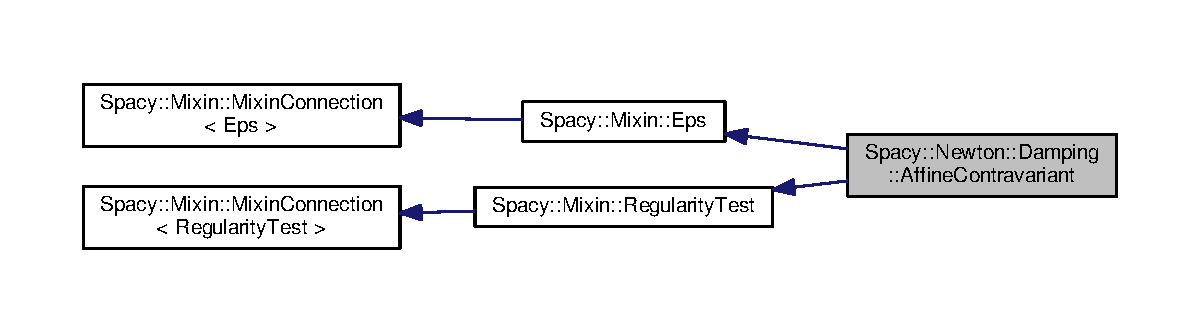
\includegraphics[width=350pt]{classSpacy_1_1Newton_1_1Damping_1_1AffineContravariant__inherit__graph}
\end{center}
\end{figure}


Collaboration diagram for Spacy\+:\+:Newton\+:\+:Damping\+:\+:Affine\+Contravariant\+:\nopagebreak
\begin{figure}[H]
\begin{center}
\leavevmode
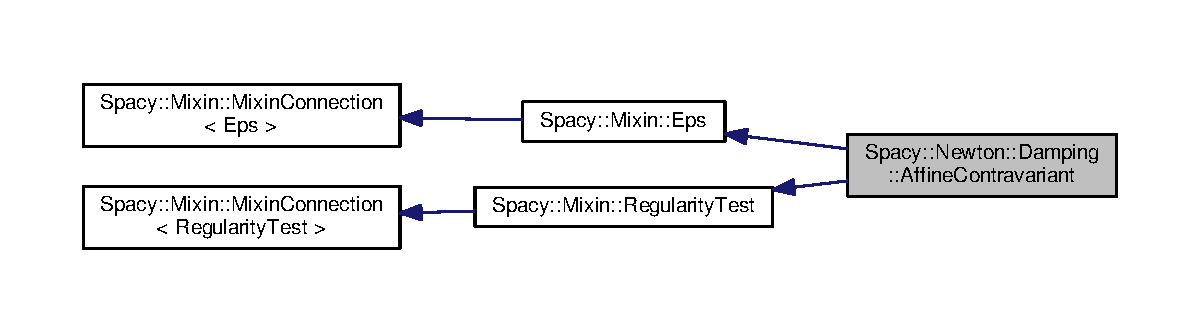
\includegraphics[width=350pt]{classSpacy_1_1Newton_1_1Damping_1_1AffineContravariant__coll__graph}
\end{center}
\end{figure}
\subsection*{Public Member Functions}
\begin{DoxyCompactItemize}
\item 
\hypertarget{classSpacy_1_1Newton_1_1Damping_1_1AffineContravariant_afbb2954f22af6d8248ec9c382a5b1ccd}{}\hyperlink{classSpacy_1_1Newton_1_1Damping_1_1AffineContravariant_afbb2954f22af6d8248ec9c382a5b1ccd}{Affine\+Contravariant} (const \hyperlink{classSpacy_1_1C1Operator}{C1\+Operator} \&F)\label{classSpacy_1_1Newton_1_1Damping_1_1AffineContravariant_afbb2954f22af6d8248ec9c382a5b1ccd}

\begin{DoxyCompactList}\small\item\em Constructor. \end{DoxyCompactList}\item 
\hypertarget{classSpacy_1_1Newton_1_1Damping_1_1AffineContravariant_a494dcf0e1c7837b4b6bd18107efcfe0b}{}\hyperlink{classSpacy_1_1DampingFactor}{Damping\+Factor} \hyperlink{classSpacy_1_1Newton_1_1Damping_1_1AffineContravariant_a494dcf0e1c7837b4b6bd18107efcfe0b}{operator()} (const std\+::function$<$ \hyperlink{classSpacy_1_1Vector}{Vector}(const \hyperlink{classSpacy_1_1Vector}{Vector} \&)$>$ \&, const \hyperlink{classSpacy_1_1Vector}{Vector} \&x, const \hyperlink{classSpacy_1_1Vector}{Vector} \&dx) const \label{classSpacy_1_1Newton_1_1Damping_1_1AffineContravariant_a494dcf0e1c7837b4b6bd18107efcfe0b}

\begin{DoxyCompactList}\small\item\em Compute damping factor. \end{DoxyCompactList}\item 
\hypertarget{classSpacy_1_1Mixin_1_1Eps_a1bbfd62541610d5d80f2782ab77158e4}{}void {\bfseries set\+Eps} (double \hyperlink{classSpacy_1_1Mixin_1_1Eps_a40e2ba8f3abd2b5370ef41238cfaaf8b}{eps})\label{classSpacy_1_1Mixin_1_1Eps_a1bbfd62541610d5d80f2782ab77158e4}

\item 
\hypertarget{classSpacy_1_1Mixin_1_1Eps_a40e2ba8f3abd2b5370ef41238cfaaf8b}{}double \hyperlink{classSpacy_1_1Mixin_1_1Eps_a40e2ba8f3abd2b5370ef41238cfaaf8b}{eps} () const noexcept\label{classSpacy_1_1Mixin_1_1Eps_a40e2ba8f3abd2b5370ef41238cfaaf8b}

\begin{DoxyCompactList}\small\item\em Access $\varepsilon$. \end{DoxyCompactList}\item 
\hypertarget{classSpacy_1_1Mixin_1_1Eps_a29e8c25dc3f1fdede57b8eb06f520fe1}{}double \hyperlink{classSpacy_1_1Mixin_1_1Eps_a29e8c25dc3f1fdede57b8eb06f520fe1}{sqrt\+Eps} () const noexcept\label{classSpacy_1_1Mixin_1_1Eps_a29e8c25dc3f1fdede57b8eb06f520fe1}

\begin{DoxyCompactList}\small\item\em Access $\sqrt\varepsilon$. \end{DoxyCompactList}\item 
\hypertarget{classSpacy_1_1Mixin_1_1Eps_a1879ebbf1b467cb4be36bcc63307018d}{}double \hyperlink{classSpacy_1_1Mixin_1_1Eps_a1879ebbf1b467cb4be36bcc63307018d}{cbrt\+Eps} () const noexcept\label{classSpacy_1_1Mixin_1_1Eps_a1879ebbf1b467cb4be36bcc63307018d}

\begin{DoxyCompactList}\small\item\em Access $\varepsilon^{1/3}$. \end{DoxyCompactList}\item 
\hypertarget{classSpacy_1_1Mixin_1_1Eps_a151216968daef3da5f5cdc0b957ce01b}{}void \hyperlink{classSpacy_1_1Mixin_1_1Eps_a151216968daef3da5f5cdc0b957ce01b}{update} (\hyperlink{classSpacy_1_1Mixin_1_1Eps_a51dbe0b9cc950e0f3dfd34a481f08ae4}{Eps} $\ast$changed\+Subject)\label{classSpacy_1_1Mixin_1_1Eps_a151216968daef3da5f5cdc0b957ce01b}

\begin{DoxyCompactList}\small\item\em update function for observer pattern. \end{DoxyCompactList}\item 
\hypertarget{classSpacy_1_1Mixin_1_1MixinConnection_abb5520ee6b22dd993d78f142939a1ed4}{}void \hyperlink{classSpacy_1_1Mixin_1_1MixinConnection_abb5520ee6b22dd993d78f142939a1ed4}{attach} (\hyperlink{classSpacy_1_1Mixin_1_1Eps_a51dbe0b9cc950e0f3dfd34a481f08ae4}{Eps} \&observer)\label{classSpacy_1_1Mixin_1_1MixinConnection_abb5520ee6b22dd993d78f142939a1ed4}

\begin{DoxyCompactList}\small\item\em Attach observer. \end{DoxyCompactList}\item 
\hypertarget{classSpacy_1_1Mixin_1_1MixinConnection_adda739590c487679c26f60e50aedb73f}{}void \hyperlink{classSpacy_1_1Mixin_1_1MixinConnection_adda739590c487679c26f60e50aedb73f}{detach} (\hyperlink{classSpacy_1_1Mixin_1_1Eps_a51dbe0b9cc950e0f3dfd34a481f08ae4}{Eps} \&observer)\label{classSpacy_1_1Mixin_1_1MixinConnection_adda739590c487679c26f60e50aedb73f}

\begin{DoxyCompactList}\small\item\em Detach observer. \end{DoxyCompactList}\item 
\hypertarget{classSpacy_1_1Mixin_1_1MixinConnection_a1ddeaa78a3bb4a38c2cca36d1f99fe36}{}void \hyperlink{classSpacy_1_1Mixin_1_1MixinConnection_a1ddeaa78a3bb4a38c2cca36d1f99fe36}{notify} ()\label{classSpacy_1_1Mixin_1_1MixinConnection_a1ddeaa78a3bb4a38c2cca36d1f99fe36}

\begin{DoxyCompactList}\small\item\em Notify observers about changes. \end{DoxyCompactList}\item 
\hypertarget{classSpacy_1_1Mixin_1_1RegularityTest_a051394f2ffb0abd9a26ab7a64c590eee}{}void \hyperlink{classSpacy_1_1Mixin_1_1RegularityTest_a051394f2ffb0abd9a26ab7a64c590eee}{set\+Lower\+Bound} (\hyperlink{classSpacy_1_1Real}{Real} lower\+Bound)\label{classSpacy_1_1Mixin_1_1RegularityTest_a051394f2ffb0abd9a26ab7a64c590eee}

\begin{DoxyCompactList}\small\item\em Set lower bound of regularity test for termination criteria. \end{DoxyCompactList}\item 
\hypertarget{classSpacy_1_1Mixin_1_1RegularityTest_a8a807e4449e6b6b64e7e81834d331597}{}\hyperlink{classSpacy_1_1Real}{Real} {\bfseries lower\+Bound} () const noexcept\label{classSpacy_1_1Mixin_1_1RegularityTest_a8a807e4449e6b6b64e7e81834d331597}

\item 
bool \hyperlink{classSpacy_1_1Mixin_1_1RegularityTest_afe2fd3259850b874a85779d4f562e7f6}{regularity\+Test\+Passed} (\hyperlink{classSpacy_1_1Real}{Real} nu) const noexcept
\begin{DoxyCompactList}\small\item\em Apply regularity test. \end{DoxyCompactList}\item 
bool \hyperlink{classSpacy_1_1Mixin_1_1RegularityTest_a26217e26765bb6f938224ea76612c8c0}{regularity\+Test\+Failed} (\hyperlink{classSpacy_1_1Real}{Real} nu) const noexcept
\begin{DoxyCompactList}\small\item\em Apply regularity test. \end{DoxyCompactList}\item 
\hypertarget{classSpacy_1_1Mixin_1_1RegularityTest_ae3bfc55bec9fe3068adffb6d24b3b964}{}void \hyperlink{classSpacy_1_1Mixin_1_1RegularityTest_ae3bfc55bec9fe3068adffb6d24b3b964}{update} (Mixin\+Connection$<$ \hyperlink{classSpacy_1_1Mixin_1_1RegularityTest_ae2887fec9a5bdd42239b3df6750bf2e9}{Regularity\+Test} $>$ $\ast$changed\+Subject)\label{classSpacy_1_1Mixin_1_1RegularityTest_ae3bfc55bec9fe3068adffb6d24b3b964}

\begin{DoxyCompactList}\small\item\em update function for observer pattern. \end{DoxyCompactList}\item 
\hypertarget{classSpacy_1_1Mixin_1_1MixinConnection_abb5520ee6b22dd993d78f142939a1ed4}{}void \hyperlink{classSpacy_1_1Mixin_1_1MixinConnection_abb5520ee6b22dd993d78f142939a1ed4}{attach} (\hyperlink{classSpacy_1_1Mixin_1_1RegularityTest_ae2887fec9a5bdd42239b3df6750bf2e9}{Regularity\+Test} \&observer)\label{classSpacy_1_1Mixin_1_1MixinConnection_abb5520ee6b22dd993d78f142939a1ed4}

\begin{DoxyCompactList}\small\item\em Attach observer. \end{DoxyCompactList}\item 
\hypertarget{classSpacy_1_1Mixin_1_1MixinConnection_adda739590c487679c26f60e50aedb73f}{}void \hyperlink{classSpacy_1_1Mixin_1_1MixinConnection_adda739590c487679c26f60e50aedb73f}{detach} (\hyperlink{classSpacy_1_1Mixin_1_1RegularityTest_ae2887fec9a5bdd42239b3df6750bf2e9}{Regularity\+Test} \&observer)\label{classSpacy_1_1Mixin_1_1MixinConnection_adda739590c487679c26f60e50aedb73f}

\begin{DoxyCompactList}\small\item\em Detach observer. \end{DoxyCompactList}\item 
\hypertarget{classSpacy_1_1Mixin_1_1MixinConnection_a1ddeaa78a3bb4a38c2cca36d1f99fe36}{}void \hyperlink{classSpacy_1_1Mixin_1_1MixinConnection_a1ddeaa78a3bb4a38c2cca36d1f99fe36}{notify} ()\label{classSpacy_1_1Mixin_1_1MixinConnection_a1ddeaa78a3bb4a38c2cca36d1f99fe36}

\begin{DoxyCompactList}\small\item\em Notify observers about changes. \end{DoxyCompactList}\end{DoxyCompactItemize}


\subsection{Detailed Description}
Affine contravariant damping strategy as described in \cite{Deuflhard2004} \mbox{[}Sec. 3.\+2\mbox{]}. 

\subsection{Member Function Documentation}
\hypertarget{classSpacy_1_1Mixin_1_1RegularityTest_afe2fd3259850b874a85779d4f562e7f6}{}\index{Spacy\+::\+Newton\+::\+Damping\+::\+Affine\+Contravariant@{Spacy\+::\+Newton\+::\+Damping\+::\+Affine\+Contravariant}!regularity\+Test\+Passed@{regularity\+Test\+Passed}}
\index{regularity\+Test\+Passed@{regularity\+Test\+Passed}!Spacy\+::\+Newton\+::\+Damping\+::\+Affine\+Contravariant@{Spacy\+::\+Newton\+::\+Damping\+::\+Affine\+Contravariant}}
\subsubsection[{regularity\+Test\+Passed}]{\setlength{\rightskip}{0pt plus 5cm}bool Spacy\+::\+Mixin\+::\+Regularity\+Test\+::regularity\+Test\+Passed (
\begin{DoxyParamCaption}
\item[{{\bf Real}}]{nu}
\end{DoxyParamCaption}
) const\hspace{0.3cm}{\ttfamily [noexcept]}, {\ttfamily [inherited]}}\label{classSpacy_1_1Mixin_1_1RegularityTest_afe2fd3259850b874a85779d4f562e7f6}


Apply regularity test. 


\begin{DoxyParams}{Parameters}
{\em nu} & damping factor \\
\hline
\end{DoxyParams}
\begin{DoxyReturn}{Returns}
$nu > lowerBound_$ 
\end{DoxyReturn}
\hypertarget{classSpacy_1_1Mixin_1_1RegularityTest_a26217e26765bb6f938224ea76612c8c0}{}\index{Spacy\+::\+Newton\+::\+Damping\+::\+Affine\+Contravariant@{Spacy\+::\+Newton\+::\+Damping\+::\+Affine\+Contravariant}!regularity\+Test\+Failed@{regularity\+Test\+Failed}}
\index{regularity\+Test\+Failed@{regularity\+Test\+Failed}!Spacy\+::\+Newton\+::\+Damping\+::\+Affine\+Contravariant@{Spacy\+::\+Newton\+::\+Damping\+::\+Affine\+Contravariant}}
\subsubsection[{regularity\+Test\+Failed}]{\setlength{\rightskip}{0pt plus 5cm}bool Spacy\+::\+Mixin\+::\+Regularity\+Test\+::regularity\+Test\+Failed (
\begin{DoxyParamCaption}
\item[{{\bf Real}}]{nu}
\end{DoxyParamCaption}
) const\hspace{0.3cm}{\ttfamily [noexcept]}, {\ttfamily [inherited]}}\label{classSpacy_1_1Mixin_1_1RegularityTest_a26217e26765bb6f938224ea76612c8c0}


Apply regularity test. 


\begin{DoxyParams}{Parameters}
{\em nu} & damping factor \\
\hline
\end{DoxyParams}
\begin{DoxyReturn}{Returns}
$nu <= lowerBound_$ 
\end{DoxyReturn}


The documentation for this class was generated from the following file\+:\begin{DoxyCompactItemize}
\item 
Spacy/\+Algorithm/\+Newton/damping\+Strategies.\+hh\end{DoxyCompactItemize}

\hypertarget{classSpacy_1_1Newton_1_1Damping_1_1AffineCovariant}{}\section{Spacy\+:\+:Newton\+:\+:Damping\+:\+:Affine\+Covariant Class Reference}
\label{classSpacy_1_1Newton_1_1Damping_1_1AffineCovariant}\index{Spacy\+::\+Newton\+::\+Damping\+::\+Affine\+Covariant@{Spacy\+::\+Newton\+::\+Damping\+::\+Affine\+Covariant}}


Affine covariant damping strategy as described in \cite{Deuflhard2004} \mbox{[}Sec. 3.\+3\mbox{]}.  




{\ttfamily \#include $<$damping\+Strategies.\+hh$>$}



Inheritance diagram for Spacy\+:\+:Newton\+:\+:Damping\+:\+:Affine\+Covariant\+:\nopagebreak
\begin{figure}[H]
\begin{center}
\leavevmode
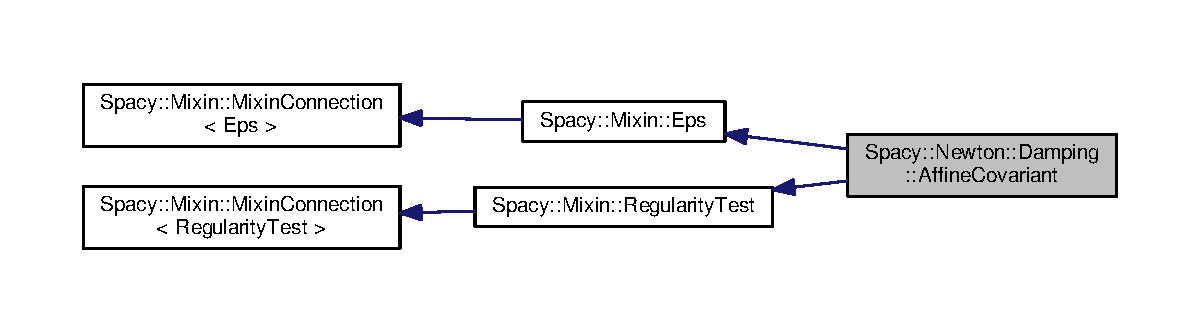
\includegraphics[width=350pt]{classSpacy_1_1Newton_1_1Damping_1_1AffineCovariant__inherit__graph}
\end{center}
\end{figure}


Collaboration diagram for Spacy\+:\+:Newton\+:\+:Damping\+:\+:Affine\+Covariant\+:\nopagebreak
\begin{figure}[H]
\begin{center}
\leavevmode
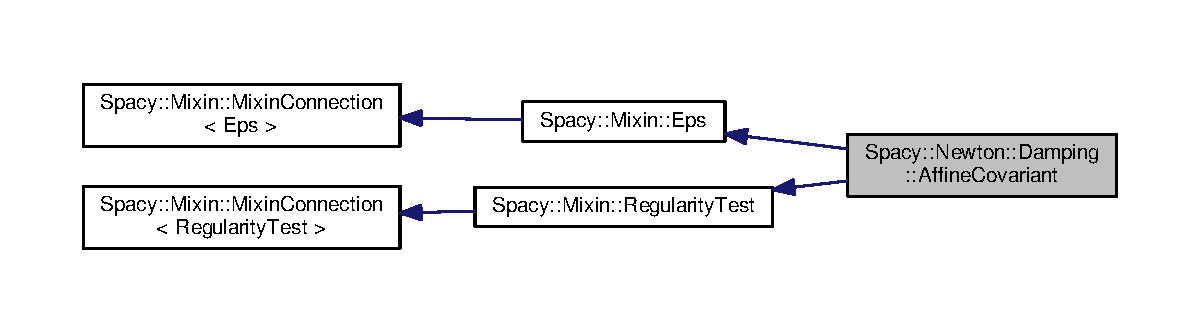
\includegraphics[width=350pt]{classSpacy_1_1Newton_1_1Damping_1_1AffineCovariant__coll__graph}
\end{center}
\end{figure}
\subsection*{Public Member Functions}
\begin{DoxyCompactItemize}
\item 
\hypertarget{classSpacy_1_1Newton_1_1Damping_1_1AffineCovariant_a316bca14949ace2b808f071a72191e5e}{}\hyperlink{classSpacy_1_1Newton_1_1Damping_1_1AffineCovariant_a316bca14949ace2b808f071a72191e5e}{Affine\+Covariant} (const \hyperlink{group__SpacyGroup_ga3f89622eba80cf840b2a7102f1303455_ga3f89622eba80cf840b2a7102f1303455}{Operator} \&F)\label{classSpacy_1_1Newton_1_1Damping_1_1AffineCovariant_a316bca14949ace2b808f071a72191e5e}

\begin{DoxyCompactList}\small\item\em Constructor. \end{DoxyCompactList}\item 
\hypertarget{classSpacy_1_1Newton_1_1Damping_1_1AffineCovariant_a6c83b5a335e93b256130c01d90499d3b}{}\hyperlink{classSpacy_1_1DampingFactor}{Damping\+Factor} \hyperlink{classSpacy_1_1Newton_1_1Damping_1_1AffineCovariant_a6c83b5a335e93b256130c01d90499d3b}{operator()} (const \hyperlink{namespaceSpacy_a7d5cd1c6fb9dd85aa345b536caf30bba_a7d5cd1c6fb9dd85aa345b536caf30bba}{Linear\+Solver} \&D\+F\+Inv\+\_\+, const \hyperlink{classSpacy_1_1Vector}{Vector} \&x, const \hyperlink{classSpacy_1_1Vector}{Vector} \&dx) const \label{classSpacy_1_1Newton_1_1Damping_1_1AffineCovariant_a6c83b5a335e93b256130c01d90499d3b}

\begin{DoxyCompactList}\small\item\em Compute damping factor. \end{DoxyCompactList}\item 
void \hyperlink{classSpacy_1_1Mixin_1_1Eps_a1bbfd62541610d5d80f2782ab77158e4_a1bbfd62541610d5d80f2782ab77158e4}{set\+Eps} (double \hyperlink{classSpacy_1_1Mixin_1_1Eps_a40e2ba8f3abd2b5370ef41238cfaaf8b_a40e2ba8f3abd2b5370ef41238cfaaf8b}{eps})
\begin{DoxyCompactList}\small\item\em Set maximal attainable accuracy $\varepsilon$. \end{DoxyCompactList}\item 
double \hyperlink{classSpacy_1_1Mixin_1_1Eps_a40e2ba8f3abd2b5370ef41238cfaaf8b_a40e2ba8f3abd2b5370ef41238cfaaf8b}{eps} () const noexcept
\begin{DoxyCompactList}\small\item\em Access maximal attainable accuracy. \end{DoxyCompactList}\item 
double \hyperlink{classSpacy_1_1Mixin_1_1Eps_a29e8c25dc3f1fdede57b8eb06f520fe1_a29e8c25dc3f1fdede57b8eb06f520fe1}{sqrt\+Eps} () const noexcept
\begin{DoxyCompactList}\small\item\em Access square root of maximal attainable accuracy. \end{DoxyCompactList}\item 
double \hyperlink{classSpacy_1_1Mixin_1_1Eps_a1879ebbf1b467cb4be36bcc63307018d_a1879ebbf1b467cb4be36bcc63307018d}{cbrt\+Eps} () const noexcept
\begin{DoxyCompactList}\small\item\em Get third root of maximal attainable accuracy. \end{DoxyCompactList}\item 
void \hyperlink{classSpacy_1_1Mixin_1_1Eps_af69cd3dee52e723302b21ca2a25f1192_af69cd3dee52e723302b21ca2a25f1192}{attach\+Eps} (\hyperlink{classSpacy_1_1Mixin_1_1Eps_a51dbe0b9cc950e0f3dfd34a481f08ae4_a51dbe0b9cc950e0f3dfd34a481f08ae4}{Eps} \&other)
\begin{DoxyCompactList}\small\item\em Attach \hyperlink{classSpacy_1_1Mixin_1_1Eps}{Eps}. \end{DoxyCompactList}\item 
\hypertarget{classSpacy_1_1Mixin_1_1Eps_ab49910e189cb86b6fd6f89b6f2af14cc}{}void \hyperlink{classSpacy_1_1Mixin_1_1Eps_ab49910e189cb86b6fd6f89b6f2af14cc}{detach\+Eps} (\hyperlink{classSpacy_1_1Mixin_1_1Eps_a51dbe0b9cc950e0f3dfd34a481f08ae4_a51dbe0b9cc950e0f3dfd34a481f08ae4}{Eps} \&other)\label{classSpacy_1_1Mixin_1_1Eps_ab49910e189cb86b6fd6f89b6f2af14cc}

\begin{DoxyCompactList}\small\item\em Detach \hyperlink{classSpacy_1_1Mixin_1_1Eps}{Eps} before it gets deleted. \end{DoxyCompactList}\item 
\hypertarget{classSpacy_1_1Mixin_1_1Eps_a151216968daef3da5f5cdc0b957ce01b}{}void \hyperlink{classSpacy_1_1Mixin_1_1Eps_a151216968daef3da5f5cdc0b957ce01b}{update} (\hyperlink{classSpacy_1_1Mixin_1_1Eps_a51dbe0b9cc950e0f3dfd34a481f08ae4_a51dbe0b9cc950e0f3dfd34a481f08ae4}{Eps} $\ast$changed\+Subject)\label{classSpacy_1_1Mixin_1_1Eps_a151216968daef3da5f5cdc0b957ce01b}

\begin{DoxyCompactList}\small\item\em update function for observer pattern. \end{DoxyCompactList}\item 
void \hyperlink{classSpacy_1_1Mixin_1_1RegularityTest_a051394f2ffb0abd9a26ab7a64c590eee_a051394f2ffb0abd9a26ab7a64c590eee}{set\+Lower\+Bound} (\hyperlink{classSpacy_1_1Real}{Real} \hyperlink{classSpacy_1_1Mixin_1_1RegularityTest_a8a807e4449e6b6b64e7e81834d331597_a8a807e4449e6b6b64e7e81834d331597}{lower\+Bound})
\begin{DoxyCompactList}\small\item\em Set lower bound of regularity test for termination criteria. \end{DoxyCompactList}\item 
\hyperlink{classSpacy_1_1Real}{Real} \hyperlink{classSpacy_1_1Mixin_1_1RegularityTest_a8a807e4449e6b6b64e7e81834d331597_a8a807e4449e6b6b64e7e81834d331597}{lower\+Bound} () const noexcept
\begin{DoxyCompactList}\small\item\em Access lower bound. \end{DoxyCompactList}\item 
bool \hyperlink{classSpacy_1_1Mixin_1_1RegularityTest_afe2fd3259850b874a85779d4f562e7f6_afe2fd3259850b874a85779d4f562e7f6}{regularity\+Test\+Passed} (\hyperlink{classSpacy_1_1Real}{Real} nu) const noexcept
\begin{DoxyCompactList}\small\item\em Apply regularity test. \end{DoxyCompactList}\item 
bool \hyperlink{classSpacy_1_1Mixin_1_1RegularityTest_a26217e26765bb6f938224ea76612c8c0_a26217e26765bb6f938224ea76612c8c0}{regularity\+Test\+Failed} (\hyperlink{classSpacy_1_1Real}{Real} nu) const noexcept
\begin{DoxyCompactList}\small\item\em Apply regularity test. \end{DoxyCompactList}\item 
void \hyperlink{classSpacy_1_1Mixin_1_1RegularityTest_aeb6598687d622ef266d1ed515d2b42bf_aeb6598687d622ef266d1ed515d2b42bf}{attach\+Regularity\+Test} (\hyperlink{classSpacy_1_1Mixin_1_1RegularityTest_ae2887fec9a5bdd42239b3df6750bf2e9_ae2887fec9a5bdd42239b3df6750bf2e9}{Regularity\+Test} \&other)
\begin{DoxyCompactList}\small\item\em Attach \hyperlink{classSpacy_1_1Mixin_1_1RegularityTest}{Regularity\+Test}. \end{DoxyCompactList}\item 
\hypertarget{classSpacy_1_1Mixin_1_1RegularityTest_a289d6422bd82864d661bdbcfc7dc321e}{}void \hyperlink{classSpacy_1_1Mixin_1_1RegularityTest_a289d6422bd82864d661bdbcfc7dc321e}{detach\+Regularity\+Test} (\hyperlink{classSpacy_1_1Mixin_1_1RegularityTest_ae2887fec9a5bdd42239b3df6750bf2e9_ae2887fec9a5bdd42239b3df6750bf2e9}{Regularity\+Test} \&other)\label{classSpacy_1_1Mixin_1_1RegularityTest_a289d6422bd82864d661bdbcfc7dc321e}

\begin{DoxyCompactList}\small\item\em Detach \hyperlink{classSpacy_1_1Mixin_1_1Eps}{Eps} before it gets deleted. \end{DoxyCompactList}\item 
\hypertarget{classSpacy_1_1Mixin_1_1RegularityTest_ae3bfc55bec9fe3068adffb6d24b3b964}{}void \hyperlink{classSpacy_1_1Mixin_1_1RegularityTest_ae3bfc55bec9fe3068adffb6d24b3b964}{update} (Mixin\+Connection$<$ \hyperlink{classSpacy_1_1Mixin_1_1RegularityTest_ae2887fec9a5bdd42239b3df6750bf2e9_ae2887fec9a5bdd42239b3df6750bf2e9}{Regularity\+Test} $>$ $\ast$changed\+Subject)\label{classSpacy_1_1Mixin_1_1RegularityTest_ae3bfc55bec9fe3068adffb6d24b3b964}

\begin{DoxyCompactList}\small\item\em update function for observer pattern. \end{DoxyCompactList}\end{DoxyCompactItemize}
\subsection*{Protected Member Functions}
\begin{DoxyCompactItemize}
\item 
\hypertarget{classSpacy_1_1Mixin_1_1MixinConnection_abb5520ee6b22dd993d78f142939a1ed4}{}void \hyperlink{classSpacy_1_1Mixin_1_1MixinConnection_abb5520ee6b22dd993d78f142939a1ed4}{attach} (\hyperlink{classSpacy_1_1Mixin_1_1Eps_a51dbe0b9cc950e0f3dfd34a481f08ae4_a51dbe0b9cc950e0f3dfd34a481f08ae4}{Eps} \&observer)\label{classSpacy_1_1Mixin_1_1MixinConnection_abb5520ee6b22dd993d78f142939a1ed4}

\begin{DoxyCompactList}\small\item\em Attach observer. \end{DoxyCompactList}\item 
\hypertarget{classSpacy_1_1Mixin_1_1MixinConnection_adda739590c487679c26f60e50aedb73f}{}void \hyperlink{classSpacy_1_1Mixin_1_1MixinConnection_adda739590c487679c26f60e50aedb73f}{detach} (\hyperlink{classSpacy_1_1Mixin_1_1Eps_a51dbe0b9cc950e0f3dfd34a481f08ae4_a51dbe0b9cc950e0f3dfd34a481f08ae4}{Eps} \&observer)\label{classSpacy_1_1Mixin_1_1MixinConnection_adda739590c487679c26f60e50aedb73f}

\begin{DoxyCompactList}\small\item\em Detach observer. \end{DoxyCompactList}\item 
\hypertarget{classSpacy_1_1Mixin_1_1MixinConnection_a1ddeaa78a3bb4a38c2cca36d1f99fe36}{}void \hyperlink{classSpacy_1_1Mixin_1_1MixinConnection_a1ddeaa78a3bb4a38c2cca36d1f99fe36}{notify} ()\label{classSpacy_1_1Mixin_1_1MixinConnection_a1ddeaa78a3bb4a38c2cca36d1f99fe36}

\begin{DoxyCompactList}\small\item\em Notify observers about changes. \end{DoxyCompactList}\item 
\hypertarget{classSpacy_1_1Mixin_1_1MixinConnection_abb5520ee6b22dd993d78f142939a1ed4}{}void \hyperlink{classSpacy_1_1Mixin_1_1MixinConnection_abb5520ee6b22dd993d78f142939a1ed4}{attach} (\hyperlink{classSpacy_1_1Mixin_1_1RegularityTest_ae2887fec9a5bdd42239b3df6750bf2e9_ae2887fec9a5bdd42239b3df6750bf2e9}{Regularity\+Test} \&observer)\label{classSpacy_1_1Mixin_1_1MixinConnection_abb5520ee6b22dd993d78f142939a1ed4}

\begin{DoxyCompactList}\small\item\em Attach observer. \end{DoxyCompactList}\item 
\hypertarget{classSpacy_1_1Mixin_1_1MixinConnection_adda739590c487679c26f60e50aedb73f}{}void \hyperlink{classSpacy_1_1Mixin_1_1MixinConnection_adda739590c487679c26f60e50aedb73f}{detach} (\hyperlink{classSpacy_1_1Mixin_1_1RegularityTest_ae2887fec9a5bdd42239b3df6750bf2e9_ae2887fec9a5bdd42239b3df6750bf2e9}{Regularity\+Test} \&observer)\label{classSpacy_1_1Mixin_1_1MixinConnection_adda739590c487679c26f60e50aedb73f}

\begin{DoxyCompactList}\small\item\em Detach observer. \end{DoxyCompactList}\item 
\hypertarget{classSpacy_1_1Mixin_1_1MixinConnection_a1ddeaa78a3bb4a38c2cca36d1f99fe36}{}void \hyperlink{classSpacy_1_1Mixin_1_1MixinConnection_a1ddeaa78a3bb4a38c2cca36d1f99fe36}{notify} ()\label{classSpacy_1_1Mixin_1_1MixinConnection_a1ddeaa78a3bb4a38c2cca36d1f99fe36}

\begin{DoxyCompactList}\small\item\em Notify observers about changes. \end{DoxyCompactList}\end{DoxyCompactItemize}


\subsection{Detailed Description}
Affine covariant damping strategy as described in \cite{Deuflhard2004} \mbox{[}Sec. 3.\+3\mbox{]}. 

\subsection{Member Function Documentation}
\hypertarget{classSpacy_1_1Mixin_1_1Eps_af69cd3dee52e723302b21ca2a25f1192_af69cd3dee52e723302b21ca2a25f1192}{}\index{Spacy\+::\+Newton\+::\+Damping\+::\+Affine\+Covariant@{Spacy\+::\+Newton\+::\+Damping\+::\+Affine\+Covariant}!attach\+Eps@{attach\+Eps}}
\index{attach\+Eps@{attach\+Eps}!Spacy\+::\+Newton\+::\+Damping\+::\+Affine\+Covariant@{Spacy\+::\+Newton\+::\+Damping\+::\+Affine\+Covariant}}
\subsubsection[{attach\+Eps}]{\setlength{\rightskip}{0pt plus 5cm}void Spacy\+::\+Mixin\+::\+Eps\+::attach\+Eps (
\begin{DoxyParamCaption}
\item[{{\bf Eps} \&}]{other}
\end{DoxyParamCaption}
)\hspace{0.3cm}{\ttfamily [inherited]}}\label{classSpacy_1_1Mixin_1_1Eps_af69cd3dee52e723302b21ca2a25f1192_af69cd3dee52e723302b21ca2a25f1192}


Attach \hyperlink{classSpacy_1_1Mixin_1_1Eps}{Eps}. 

When \hyperlink{classSpacy_1_1Mixin_1_1Eps_a1bbfd62541610d5d80f2782ab77158e4_a1bbfd62541610d5d80f2782ab77158e4}{set\+Eps(double eps)} is called, then also other.\+set\+Eps(eps) is invoked. \hypertarget{classSpacy_1_1Mixin_1_1RegularityTest_aeb6598687d622ef266d1ed515d2b42bf_aeb6598687d622ef266d1ed515d2b42bf}{}\index{Spacy\+::\+Newton\+::\+Damping\+::\+Affine\+Covariant@{Spacy\+::\+Newton\+::\+Damping\+::\+Affine\+Covariant}!attach\+Regularity\+Test@{attach\+Regularity\+Test}}
\index{attach\+Regularity\+Test@{attach\+Regularity\+Test}!Spacy\+::\+Newton\+::\+Damping\+::\+Affine\+Covariant@{Spacy\+::\+Newton\+::\+Damping\+::\+Affine\+Covariant}}
\subsubsection[{attach\+Regularity\+Test}]{\setlength{\rightskip}{0pt plus 5cm}void Spacy\+::\+Mixin\+::\+Regularity\+Test\+::attach\+Regularity\+Test (
\begin{DoxyParamCaption}
\item[{{\bf Regularity\+Test} \&}]{other}
\end{DoxyParamCaption}
)\hspace{0.3cm}{\ttfamily [inherited]}}\label{classSpacy_1_1Mixin_1_1RegularityTest_aeb6598687d622ef266d1ed515d2b42bf_aeb6598687d622ef266d1ed515d2b42bf}


Attach \hyperlink{classSpacy_1_1Mixin_1_1RegularityTest}{Regularity\+Test}. 

When set\+Lower\+Bound(double lower\+Bound) is called, then also other.\+set\+Lower\+Bound(lower\+Bound) is invoked. \hypertarget{classSpacy_1_1Mixin_1_1Eps_a1879ebbf1b467cb4be36bcc63307018d_a1879ebbf1b467cb4be36bcc63307018d}{}\index{Spacy\+::\+Newton\+::\+Damping\+::\+Affine\+Covariant@{Spacy\+::\+Newton\+::\+Damping\+::\+Affine\+Covariant}!cbrt\+Eps@{cbrt\+Eps}}
\index{cbrt\+Eps@{cbrt\+Eps}!Spacy\+::\+Newton\+::\+Damping\+::\+Affine\+Covariant@{Spacy\+::\+Newton\+::\+Damping\+::\+Affine\+Covariant}}
\subsubsection[{cbrt\+Eps}]{\setlength{\rightskip}{0pt plus 5cm}double Spacy\+::\+Mixin\+::\+Eps\+::cbrt\+Eps (
\begin{DoxyParamCaption}
{}
\end{DoxyParamCaption}
) const\hspace{0.3cm}{\ttfamily [noexcept]}, {\ttfamily [inherited]}}\label{classSpacy_1_1Mixin_1_1Eps_a1879ebbf1b467cb4be36bcc63307018d_a1879ebbf1b467cb4be36bcc63307018d}


Get third root of maximal attainable accuracy. 

\begin{DoxyReturn}{Returns}
$\varepsilon^{1/3}$ 
\end{DoxyReturn}
\hypertarget{classSpacy_1_1Mixin_1_1Eps_a40e2ba8f3abd2b5370ef41238cfaaf8b_a40e2ba8f3abd2b5370ef41238cfaaf8b}{}\index{Spacy\+::\+Newton\+::\+Damping\+::\+Affine\+Covariant@{Spacy\+::\+Newton\+::\+Damping\+::\+Affine\+Covariant}!eps@{eps}}
\index{eps@{eps}!Spacy\+::\+Newton\+::\+Damping\+::\+Affine\+Covariant@{Spacy\+::\+Newton\+::\+Damping\+::\+Affine\+Covariant}}
\subsubsection[{eps}]{\setlength{\rightskip}{0pt plus 5cm}double Spacy\+::\+Mixin\+::\+Eps\+::eps (
\begin{DoxyParamCaption}
{}
\end{DoxyParamCaption}
) const\hspace{0.3cm}{\ttfamily [noexcept]}, {\ttfamily [inherited]}}\label{classSpacy_1_1Mixin_1_1Eps_a40e2ba8f3abd2b5370ef41238cfaaf8b_a40e2ba8f3abd2b5370ef41238cfaaf8b}


Access maximal attainable accuracy. 

\begin{DoxyReturn}{Returns}
$\varepsilon$ 
\end{DoxyReturn}
\hypertarget{classSpacy_1_1Mixin_1_1RegularityTest_a8a807e4449e6b6b64e7e81834d331597_a8a807e4449e6b6b64e7e81834d331597}{}\index{Spacy\+::\+Newton\+::\+Damping\+::\+Affine\+Covariant@{Spacy\+::\+Newton\+::\+Damping\+::\+Affine\+Covariant}!lower\+Bound@{lower\+Bound}}
\index{lower\+Bound@{lower\+Bound}!Spacy\+::\+Newton\+::\+Damping\+::\+Affine\+Covariant@{Spacy\+::\+Newton\+::\+Damping\+::\+Affine\+Covariant}}
\subsubsection[{lower\+Bound}]{\setlength{\rightskip}{0pt plus 5cm}{\bf Real} Spacy\+::\+Mixin\+::\+Regularity\+Test\+::lower\+Bound (
\begin{DoxyParamCaption}
{}
\end{DoxyParamCaption}
) const\hspace{0.3cm}{\ttfamily [noexcept]}, {\ttfamily [inherited]}}\label{classSpacy_1_1Mixin_1_1RegularityTest_a8a807e4449e6b6b64e7e81834d331597_a8a807e4449e6b6b64e7e81834d331597}


Access lower bound. 

\begin{DoxyReturn}{Returns}
lower bound 
\end{DoxyReturn}
\hypertarget{classSpacy_1_1Mixin_1_1RegularityTest_a26217e26765bb6f938224ea76612c8c0_a26217e26765bb6f938224ea76612c8c0}{}\index{Spacy\+::\+Newton\+::\+Damping\+::\+Affine\+Covariant@{Spacy\+::\+Newton\+::\+Damping\+::\+Affine\+Covariant}!regularity\+Test\+Failed@{regularity\+Test\+Failed}}
\index{regularity\+Test\+Failed@{regularity\+Test\+Failed}!Spacy\+::\+Newton\+::\+Damping\+::\+Affine\+Covariant@{Spacy\+::\+Newton\+::\+Damping\+::\+Affine\+Covariant}}
\subsubsection[{regularity\+Test\+Failed}]{\setlength{\rightskip}{0pt plus 5cm}bool Spacy\+::\+Mixin\+::\+Regularity\+Test\+::regularity\+Test\+Failed (
\begin{DoxyParamCaption}
\item[{{\bf Real}}]{nu}
\end{DoxyParamCaption}
) const\hspace{0.3cm}{\ttfamily [noexcept]}, {\ttfamily [inherited]}}\label{classSpacy_1_1Mixin_1_1RegularityTest_a26217e26765bb6f938224ea76612c8c0_a26217e26765bb6f938224ea76612c8c0}


Apply regularity test. 


\begin{DoxyParams}{Parameters}
{\em nu} & damping factor \\
\hline
\end{DoxyParams}
\begin{DoxyReturn}{Returns}
$nu <= lowerBound_$ 
\end{DoxyReturn}
\hypertarget{classSpacy_1_1Mixin_1_1RegularityTest_afe2fd3259850b874a85779d4f562e7f6_afe2fd3259850b874a85779d4f562e7f6}{}\index{Spacy\+::\+Newton\+::\+Damping\+::\+Affine\+Covariant@{Spacy\+::\+Newton\+::\+Damping\+::\+Affine\+Covariant}!regularity\+Test\+Passed@{regularity\+Test\+Passed}}
\index{regularity\+Test\+Passed@{regularity\+Test\+Passed}!Spacy\+::\+Newton\+::\+Damping\+::\+Affine\+Covariant@{Spacy\+::\+Newton\+::\+Damping\+::\+Affine\+Covariant}}
\subsubsection[{regularity\+Test\+Passed}]{\setlength{\rightskip}{0pt plus 5cm}bool Spacy\+::\+Mixin\+::\+Regularity\+Test\+::regularity\+Test\+Passed (
\begin{DoxyParamCaption}
\item[{{\bf Real}}]{nu}
\end{DoxyParamCaption}
) const\hspace{0.3cm}{\ttfamily [noexcept]}, {\ttfamily [inherited]}}\label{classSpacy_1_1Mixin_1_1RegularityTest_afe2fd3259850b874a85779d4f562e7f6_afe2fd3259850b874a85779d4f562e7f6}


Apply regularity test. 


\begin{DoxyParams}{Parameters}
{\em nu} & damping factor \\
\hline
\end{DoxyParams}
\begin{DoxyReturn}{Returns}
$nu > lowerBound_$ 
\end{DoxyReturn}
\hypertarget{classSpacy_1_1Mixin_1_1Eps_a1bbfd62541610d5d80f2782ab77158e4_a1bbfd62541610d5d80f2782ab77158e4}{}\index{Spacy\+::\+Newton\+::\+Damping\+::\+Affine\+Covariant@{Spacy\+::\+Newton\+::\+Damping\+::\+Affine\+Covariant}!set\+Eps@{set\+Eps}}
\index{set\+Eps@{set\+Eps}!Spacy\+::\+Newton\+::\+Damping\+::\+Affine\+Covariant@{Spacy\+::\+Newton\+::\+Damping\+::\+Affine\+Covariant}}
\subsubsection[{set\+Eps}]{\setlength{\rightskip}{0pt plus 5cm}void Spacy\+::\+Mixin\+::\+Eps\+::set\+Eps (
\begin{DoxyParamCaption}
\item[{double}]{eps}
\end{DoxyParamCaption}
)\hspace{0.3cm}{\ttfamily [inherited]}}\label{classSpacy_1_1Mixin_1_1Eps_a1bbfd62541610d5d80f2782ab77158e4_a1bbfd62541610d5d80f2782ab77158e4}


Set maximal attainable accuracy $\varepsilon$. 


\begin{DoxyParams}{Parameters}
{\em eps} & new maximal attainable accuracy \\
\hline
\end{DoxyParams}
\hypertarget{classSpacy_1_1Mixin_1_1RegularityTest_a051394f2ffb0abd9a26ab7a64c590eee_a051394f2ffb0abd9a26ab7a64c590eee}{}\index{Spacy\+::\+Newton\+::\+Damping\+::\+Affine\+Covariant@{Spacy\+::\+Newton\+::\+Damping\+::\+Affine\+Covariant}!set\+Lower\+Bound@{set\+Lower\+Bound}}
\index{set\+Lower\+Bound@{set\+Lower\+Bound}!Spacy\+::\+Newton\+::\+Damping\+::\+Affine\+Covariant@{Spacy\+::\+Newton\+::\+Damping\+::\+Affine\+Covariant}}
\subsubsection[{set\+Lower\+Bound}]{\setlength{\rightskip}{0pt plus 5cm}void Spacy\+::\+Mixin\+::\+Regularity\+Test\+::set\+Lower\+Bound (
\begin{DoxyParamCaption}
\item[{{\bf Real}}]{lower\+Bound}
\end{DoxyParamCaption}
)\hspace{0.3cm}{\ttfamily [inherited]}}\label{classSpacy_1_1Mixin_1_1RegularityTest_a051394f2ffb0abd9a26ab7a64c590eee_a051394f2ffb0abd9a26ab7a64c590eee}


Set lower bound of regularity test for termination criteria. 


\begin{DoxyParams}{Parameters}
{\em lower\+Bound} & new lower bound \\
\hline
\end{DoxyParams}
\hypertarget{classSpacy_1_1Mixin_1_1Eps_a29e8c25dc3f1fdede57b8eb06f520fe1_a29e8c25dc3f1fdede57b8eb06f520fe1}{}\index{Spacy\+::\+Newton\+::\+Damping\+::\+Affine\+Covariant@{Spacy\+::\+Newton\+::\+Damping\+::\+Affine\+Covariant}!sqrt\+Eps@{sqrt\+Eps}}
\index{sqrt\+Eps@{sqrt\+Eps}!Spacy\+::\+Newton\+::\+Damping\+::\+Affine\+Covariant@{Spacy\+::\+Newton\+::\+Damping\+::\+Affine\+Covariant}}
\subsubsection[{sqrt\+Eps}]{\setlength{\rightskip}{0pt plus 5cm}double Spacy\+::\+Mixin\+::\+Eps\+::sqrt\+Eps (
\begin{DoxyParamCaption}
{}
\end{DoxyParamCaption}
) const\hspace{0.3cm}{\ttfamily [noexcept]}, {\ttfamily [inherited]}}\label{classSpacy_1_1Mixin_1_1Eps_a29e8c25dc3f1fdede57b8eb06f520fe1_a29e8c25dc3f1fdede57b8eb06f520fe1}


Access square root of maximal attainable accuracy. 

\begin{DoxyReturn}{Returns}
$\sqrt\varepsilon$ 
\end{DoxyReturn}


The documentation for this class was generated from the following file\+:\begin{DoxyCompactItemize}
\item 
Spacy/\+Algorithm/\+Newton/damping\+Strategies.\+hh\end{DoxyCompactItemize}

\hypertarget{classSpacy_1_1Newton_1_1Termination_1_1AffineCovariant}{}\section{Spacy\+:\+:Newton\+:\+:Termination\+:\+:Affine\+Covariant Class Reference}
\label{classSpacy_1_1Newton_1_1Termination_1_1AffineCovariant}\index{Spacy\+::\+Newton\+::\+Termination\+::\+Affine\+Covariant@{Spacy\+::\+Newton\+::\+Termination\+::\+Affine\+Covariant}}


Affine covariant relative error criterion.  




{\ttfamily \#include $<$termination\+Criteria.\+hh$>$}



Inheritance diagram for Spacy\+:\+:Newton\+:\+:Termination\+:\+:Affine\+Covariant\+:\nopagebreak
\begin{figure}[H]
\begin{center}
\leavevmode
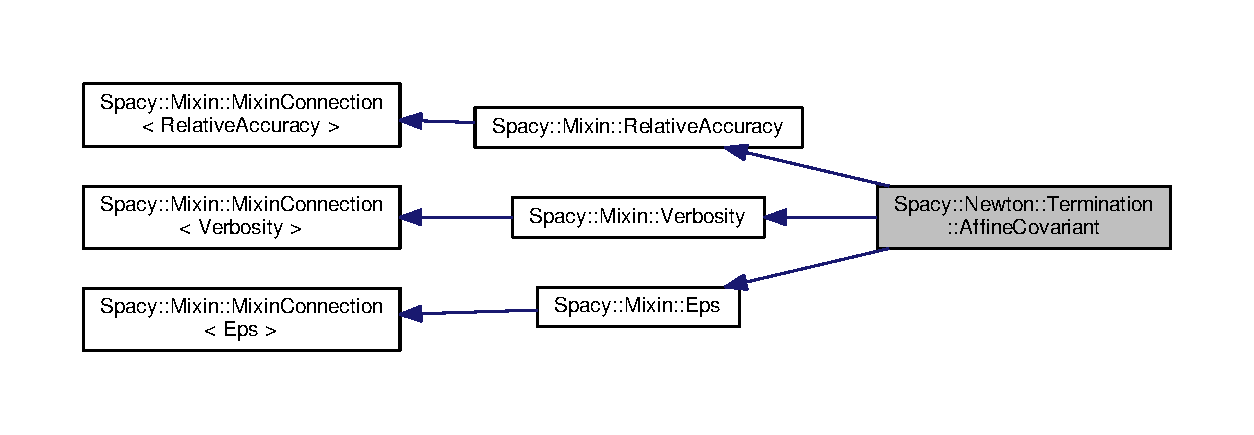
\includegraphics[width=350pt]{classSpacy_1_1Newton_1_1Termination_1_1AffineCovariant__inherit__graph}
\end{center}
\end{figure}


Collaboration diagram for Spacy\+:\+:Newton\+:\+:Termination\+:\+:Affine\+Covariant\+:\nopagebreak
\begin{figure}[H]
\begin{center}
\leavevmode
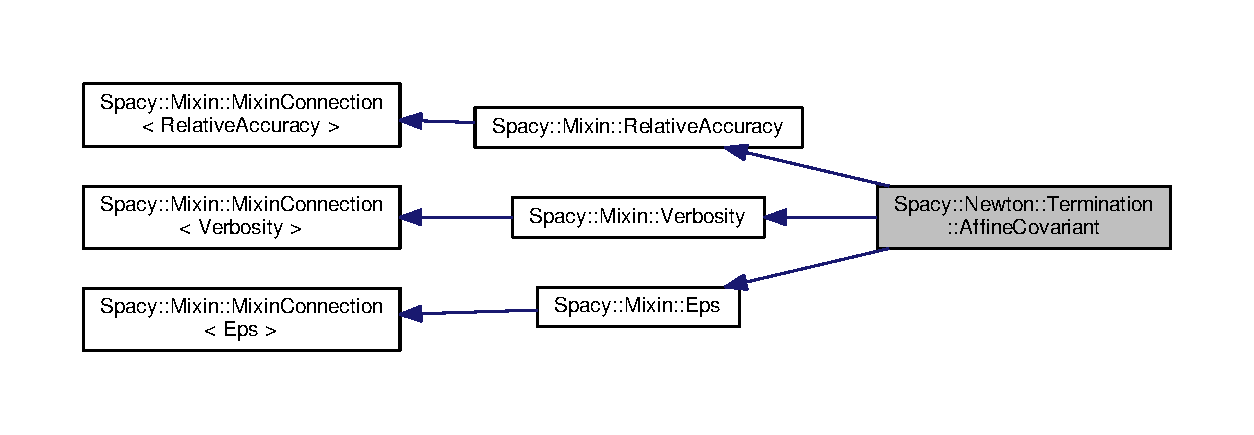
\includegraphics[width=350pt]{classSpacy_1_1Newton_1_1Termination_1_1AffineCovariant__coll__graph}
\end{center}
\end{figure}
\subsection*{Public Member Functions}
\begin{DoxyCompactItemize}
\item 
\hypertarget{classSpacy_1_1Newton_1_1Termination_1_1AffineCovariant_ae9e4098a5bdb4ad54a9f49f278fd2c39}{}\hyperlink{classSpacy_1_1Newton_1_1Termination_1_1AffineCovariant_ae9e4098a5bdb4ad54a9f49f278fd2c39}{Affine\+Covariant} (const \hyperlink{classSpacy_1_1C1Operator}{C1\+Operator} \&, double relative\+Accuracy, bool \hyperlink{classSpacy_1_1Mixin_1_1Verbosity_ad367a7328578546938fd2a7e52ab3793}{verbose}=false)\label{classSpacy_1_1Newton_1_1Termination_1_1AffineCovariant_ae9e4098a5bdb4ad54a9f49f278fd2c39}

\begin{DoxyCompactList}\small\item\em Constuctor. \end{DoxyCompactList}\item 
bool \hyperlink{classSpacy_1_1Newton_1_1Termination_1_1AffineCovariant_aa33460372120d1ddcd3daf7c79140dcf}{operator()} (\hyperlink{classSpacy_1_1DampingFactor}{Damping\+Factor} nu, const \hyperlink{classSpacy_1_1Vector}{Vector} \&x, const \hyperlink{classSpacy_1_1Vector}{Vector} \&dx) const 
\begin{DoxyCompactList}\small\item\em Apply termination criterion. \end{DoxyCompactList}\item 
\hypertarget{classSpacy_1_1Mixin_1_1RelativeAccuracy_aee88b71e80aca446a179f1310408a1e3}{}void {\bfseries set\+Relative\+Accuracy} (double accuracy)\label{classSpacy_1_1Mixin_1_1RelativeAccuracy_aee88b71e80aca446a179f1310408a1e3}

\item 
\hypertarget{classSpacy_1_1Mixin_1_1RelativeAccuracy_a1da618cf9265c2edae354524df4a7f8a}{}double {\bfseries relative\+Accuracy} () const noexcept\label{classSpacy_1_1Mixin_1_1RelativeAccuracy_a1da618cf9265c2edae354524df4a7f8a}

\item 
\hypertarget{classSpacy_1_1Mixin_1_1RelativeAccuracy_acf0b58224d9a2879d05b5d2947f37527}{}void \hyperlink{classSpacy_1_1Mixin_1_1RelativeAccuracy_acf0b58224d9a2879d05b5d2947f37527}{update} (Relative\+Accuracy $\ast$changed\+Subject)\label{classSpacy_1_1Mixin_1_1RelativeAccuracy_acf0b58224d9a2879d05b5d2947f37527}

\begin{DoxyCompactList}\small\item\em update function for observer pattern. \end{DoxyCompactList}\item 
\hypertarget{classSpacy_1_1Mixin_1_1MixinConnection_abb5520ee6b22dd993d78f142939a1ed4}{}void \hyperlink{classSpacy_1_1Mixin_1_1MixinConnection_abb5520ee6b22dd993d78f142939a1ed4}{attach} (Relative\+Accuracy \&observer)\label{classSpacy_1_1Mixin_1_1MixinConnection_abb5520ee6b22dd993d78f142939a1ed4}

\begin{DoxyCompactList}\small\item\em Attach observer. \end{DoxyCompactList}\item 
\hypertarget{classSpacy_1_1Mixin_1_1MixinConnection_adda739590c487679c26f60e50aedb73f}{}void \hyperlink{classSpacy_1_1Mixin_1_1MixinConnection_adda739590c487679c26f60e50aedb73f}{detach} (Relative\+Accuracy \&observer)\label{classSpacy_1_1Mixin_1_1MixinConnection_adda739590c487679c26f60e50aedb73f}

\begin{DoxyCompactList}\small\item\em Detach observer. \end{DoxyCompactList}\item 
\hypertarget{classSpacy_1_1Mixin_1_1MixinConnection_a1ddeaa78a3bb4a38c2cca36d1f99fe36}{}void \hyperlink{classSpacy_1_1Mixin_1_1MixinConnection_a1ddeaa78a3bb4a38c2cca36d1f99fe36}{notify} ()\label{classSpacy_1_1Mixin_1_1MixinConnection_a1ddeaa78a3bb4a38c2cca36d1f99fe36}

\begin{DoxyCompactList}\small\item\em Notify observers about changes. \end{DoxyCompactList}\item 
void \hyperlink{classSpacy_1_1Mixin_1_1Verbosity_a0365d293ab27e27da9496c668020aefb}{set\+Verbosity} (bool \hyperlink{classSpacy_1_1Mixin_1_1Verbosity_ad367a7328578546938fd2a7e52ab3793}{verbose})
\begin{DoxyCompactList}\small\item\em Enable/disable verbosity. \end{DoxyCompactList}\item 
\hypertarget{classSpacy_1_1Mixin_1_1Verbosity_ad367a7328578546938fd2a7e52ab3793}{}bool \hyperlink{classSpacy_1_1Mixin_1_1Verbosity_ad367a7328578546938fd2a7e52ab3793}{verbose} () const noexcept\label{classSpacy_1_1Mixin_1_1Verbosity_ad367a7328578546938fd2a7e52ab3793}

\begin{DoxyCompactList}\small\item\em Check if verbosity\+Level $>$ 0. \end{DoxyCompactList}\item 
\hypertarget{classSpacy_1_1Mixin_1_1Verbosity_af84a4b3c933f252a5840ab63d4a38325}{}void {\bfseries set\+Verbosity\+Level} (unsigned level) noexcept\label{classSpacy_1_1Mixin_1_1Verbosity_af84a4b3c933f252a5840ab63d4a38325}

\item 
\hypertarget{classSpacy_1_1Mixin_1_1Verbosity_a2131f495d276c95d2d6534a6dfce6f9f}{}unsigned \hyperlink{classSpacy_1_1Mixin_1_1Verbosity_a2131f495d276c95d2d6534a6dfce6f9f}{verbosity\+Level} () const noexcept\label{classSpacy_1_1Mixin_1_1Verbosity_a2131f495d276c95d2d6534a6dfce6f9f}

\begin{DoxyCompactList}\small\item\em Access verbosity level. \end{DoxyCompactList}\item 
\hypertarget{classSpacy_1_1Mixin_1_1Verbosity_a8cff860c587fcda2cdc86ba744302b33}{}void \hyperlink{classSpacy_1_1Mixin_1_1Verbosity_a8cff860c587fcda2cdc86ba744302b33}{update} (\hyperlink{classSpacy_1_1Mixin_1_1Verbosity_aefe2f237b0456c4bced001fbfa75f92e}{Verbosity} $\ast$changed\+Subject)\label{classSpacy_1_1Mixin_1_1Verbosity_a8cff860c587fcda2cdc86ba744302b33}

\begin{DoxyCompactList}\small\item\em update function for observer pattern. \end{DoxyCompactList}\item 
\hypertarget{classSpacy_1_1Mixin_1_1MixinConnection_abb5520ee6b22dd993d78f142939a1ed4}{}void \hyperlink{classSpacy_1_1Mixin_1_1MixinConnection_abb5520ee6b22dd993d78f142939a1ed4}{attach} (\hyperlink{classSpacy_1_1Mixin_1_1Verbosity_aefe2f237b0456c4bced001fbfa75f92e}{Verbosity} \&observer)\label{classSpacy_1_1Mixin_1_1MixinConnection_abb5520ee6b22dd993d78f142939a1ed4}

\begin{DoxyCompactList}\small\item\em Attach observer. \end{DoxyCompactList}\item 
\hypertarget{classSpacy_1_1Mixin_1_1MixinConnection_adda739590c487679c26f60e50aedb73f}{}void \hyperlink{classSpacy_1_1Mixin_1_1MixinConnection_adda739590c487679c26f60e50aedb73f}{detach} (\hyperlink{classSpacy_1_1Mixin_1_1Verbosity_aefe2f237b0456c4bced001fbfa75f92e}{Verbosity} \&observer)\label{classSpacy_1_1Mixin_1_1MixinConnection_adda739590c487679c26f60e50aedb73f}

\begin{DoxyCompactList}\small\item\em Detach observer. \end{DoxyCompactList}\item 
\hypertarget{classSpacy_1_1Mixin_1_1MixinConnection_a1ddeaa78a3bb4a38c2cca36d1f99fe36}{}void \hyperlink{classSpacy_1_1Mixin_1_1MixinConnection_a1ddeaa78a3bb4a38c2cca36d1f99fe36}{notify} ()\label{classSpacy_1_1Mixin_1_1MixinConnection_a1ddeaa78a3bb4a38c2cca36d1f99fe36}

\begin{DoxyCompactList}\small\item\em Notify observers about changes. \end{DoxyCompactList}\item 
\hypertarget{classSpacy_1_1Mixin_1_1Eps_a1bbfd62541610d5d80f2782ab77158e4}{}void {\bfseries set\+Eps} (double \hyperlink{classSpacy_1_1Mixin_1_1Eps_a40e2ba8f3abd2b5370ef41238cfaaf8b}{eps})\label{classSpacy_1_1Mixin_1_1Eps_a1bbfd62541610d5d80f2782ab77158e4}

\item 
\hypertarget{classSpacy_1_1Mixin_1_1Eps_a40e2ba8f3abd2b5370ef41238cfaaf8b}{}double \hyperlink{classSpacy_1_1Mixin_1_1Eps_a40e2ba8f3abd2b5370ef41238cfaaf8b}{eps} () const noexcept\label{classSpacy_1_1Mixin_1_1Eps_a40e2ba8f3abd2b5370ef41238cfaaf8b}

\begin{DoxyCompactList}\small\item\em Access $\varepsilon$. \end{DoxyCompactList}\item 
\hypertarget{classSpacy_1_1Mixin_1_1Eps_a29e8c25dc3f1fdede57b8eb06f520fe1}{}double \hyperlink{classSpacy_1_1Mixin_1_1Eps_a29e8c25dc3f1fdede57b8eb06f520fe1}{sqrt\+Eps} () const noexcept\label{classSpacy_1_1Mixin_1_1Eps_a29e8c25dc3f1fdede57b8eb06f520fe1}

\begin{DoxyCompactList}\small\item\em Access $\sqrt\varepsilon$. \end{DoxyCompactList}\item 
\hypertarget{classSpacy_1_1Mixin_1_1Eps_a1879ebbf1b467cb4be36bcc63307018d}{}double \hyperlink{classSpacy_1_1Mixin_1_1Eps_a1879ebbf1b467cb4be36bcc63307018d}{cbrt\+Eps} () const noexcept\label{classSpacy_1_1Mixin_1_1Eps_a1879ebbf1b467cb4be36bcc63307018d}

\begin{DoxyCompactList}\small\item\em Access $\varepsilon^{1/3}$. \end{DoxyCompactList}\item 
\hypertarget{classSpacy_1_1Mixin_1_1Eps_a151216968daef3da5f5cdc0b957ce01b}{}void \hyperlink{classSpacy_1_1Mixin_1_1Eps_a151216968daef3da5f5cdc0b957ce01b}{update} (\hyperlink{classSpacy_1_1Mixin_1_1Eps_a51dbe0b9cc950e0f3dfd34a481f08ae4}{Eps} $\ast$changed\+Subject)\label{classSpacy_1_1Mixin_1_1Eps_a151216968daef3da5f5cdc0b957ce01b}

\begin{DoxyCompactList}\small\item\em update function for observer pattern. \end{DoxyCompactList}\item 
\hypertarget{classSpacy_1_1Mixin_1_1MixinConnection_abb5520ee6b22dd993d78f142939a1ed4}{}void \hyperlink{classSpacy_1_1Mixin_1_1MixinConnection_abb5520ee6b22dd993d78f142939a1ed4}{attach} (\hyperlink{classSpacy_1_1Mixin_1_1Eps_a51dbe0b9cc950e0f3dfd34a481f08ae4}{Eps} \&observer)\label{classSpacy_1_1Mixin_1_1MixinConnection_abb5520ee6b22dd993d78f142939a1ed4}

\begin{DoxyCompactList}\small\item\em Attach observer. \end{DoxyCompactList}\item 
\hypertarget{classSpacy_1_1Mixin_1_1MixinConnection_adda739590c487679c26f60e50aedb73f}{}void \hyperlink{classSpacy_1_1Mixin_1_1MixinConnection_adda739590c487679c26f60e50aedb73f}{detach} (\hyperlink{classSpacy_1_1Mixin_1_1Eps_a51dbe0b9cc950e0f3dfd34a481f08ae4}{Eps} \&observer)\label{classSpacy_1_1Mixin_1_1MixinConnection_adda739590c487679c26f60e50aedb73f}

\begin{DoxyCompactList}\small\item\em Detach observer. \end{DoxyCompactList}\item 
\hypertarget{classSpacy_1_1Mixin_1_1MixinConnection_a1ddeaa78a3bb4a38c2cca36d1f99fe36}{}void \hyperlink{classSpacy_1_1Mixin_1_1MixinConnection_a1ddeaa78a3bb4a38c2cca36d1f99fe36}{notify} ()\label{classSpacy_1_1Mixin_1_1MixinConnection_a1ddeaa78a3bb4a38c2cca36d1f99fe36}

\begin{DoxyCompactList}\small\item\em Notify observers about changes. \end{DoxyCompactList}\end{DoxyCompactItemize}


\subsection{Detailed Description}
Affine covariant relative error criterion. 

\subsection{Member Function Documentation}
\hypertarget{classSpacy_1_1Newton_1_1Termination_1_1AffineCovariant_aa33460372120d1ddcd3daf7c79140dcf}{}\index{Spacy\+::\+Newton\+::\+Termination\+::\+Affine\+Covariant@{Spacy\+::\+Newton\+::\+Termination\+::\+Affine\+Covariant}!operator()@{operator()}}
\index{operator()@{operator()}!Spacy\+::\+Newton\+::\+Termination\+::\+Affine\+Covariant@{Spacy\+::\+Newton\+::\+Termination\+::\+Affine\+Covariant}}
\subsubsection[{operator()}]{\setlength{\rightskip}{0pt plus 5cm}bool Spacy\+::\+Newton\+::\+Termination\+::\+Affine\+Covariant\+::operator() (
\begin{DoxyParamCaption}
\item[{{\bf Damping\+Factor}}]{nu, }
\item[{const {\bf Vector} \&}]{x, }
\item[{const {\bf Vector} \&}]{dx}
\end{DoxyParamCaption}
) const}\label{classSpacy_1_1Newton_1_1Termination_1_1AffineCovariant_aa33460372120d1ddcd3daf7c79140dcf}


Apply termination criterion. 


\begin{DoxyParams}{Parameters}
{\em nu} & damping factor \\
\hline
{\em x} & iterate \\
\hline
{\em dx} & correction \\
\hline
\end{DoxyParams}
\begin{DoxyReturn}{Returns}
true if $\nu=1$ and $ \|dx\|<rel_acc\|x\| $ or $\|x\|=\|dx\|=0$, else false 
\end{DoxyReturn}
\hypertarget{classSpacy_1_1Mixin_1_1Verbosity_a0365d293ab27e27da9496c668020aefb}{}\index{Spacy\+::\+Newton\+::\+Termination\+::\+Affine\+Covariant@{Spacy\+::\+Newton\+::\+Termination\+::\+Affine\+Covariant}!set\+Verbosity@{set\+Verbosity}}
\index{set\+Verbosity@{set\+Verbosity}!Spacy\+::\+Newton\+::\+Termination\+::\+Affine\+Covariant@{Spacy\+::\+Newton\+::\+Termination\+::\+Affine\+Covariant}}
\subsubsection[{set\+Verbosity}]{\setlength{\rightskip}{0pt plus 5cm}void Spacy\+::\+Mixin\+::\+Verbosity\+::set\+Verbosity (
\begin{DoxyParamCaption}
\item[{bool}]{verbose}
\end{DoxyParamCaption}
)\hspace{0.3cm}{\ttfamily [inherited]}}\label{classSpacy_1_1Mixin_1_1Verbosity_a0365d293ab27e27da9496c668020aefb}


Enable/disable verbosity. 


\begin{DoxyParams}{Parameters}
{\em verbose} & true\+: if verbosity\+Level = 0, set verbosity\+Level = 1; false\+: if set verbosity\+Level = 0 \\
\hline
\end{DoxyParams}


The documentation for this class was generated from the following file\+:\begin{DoxyCompactItemize}
\item 
Spacy/\+Algorithm/\+Newton/termination\+Criteria.\+hh\end{DoxyCompactItemize}

\hypertarget{classSpacy_1_1CompositeStep_1_1AffineCovariantSolver}{}\section{Spacy\+:\+:Composite\+Step\+:\+:Affine\+Covariant\+Solver Class Reference}
\label{classSpacy_1_1CompositeStep_1_1AffineCovariantSolver}\index{Spacy\+::\+Composite\+Step\+::\+Affine\+Covariant\+Solver@{Spacy\+::\+Composite\+Step\+::\+Affine\+Covariant\+Solver}}


The affine covariant step method described in \cite{Lubkoll2015}, \cite{Lubkoll2015a} for the solution of equality constraint optimization problems.  




{\ttfamily \#include $<$affine\+Covariant\+Solver.\+hh$>$}



Inheritance diagram for Spacy\+:\+:Composite\+Step\+:\+:Affine\+Covariant\+Solver\+:\nopagebreak
\begin{figure}[H]
\begin{center}
\leavevmode
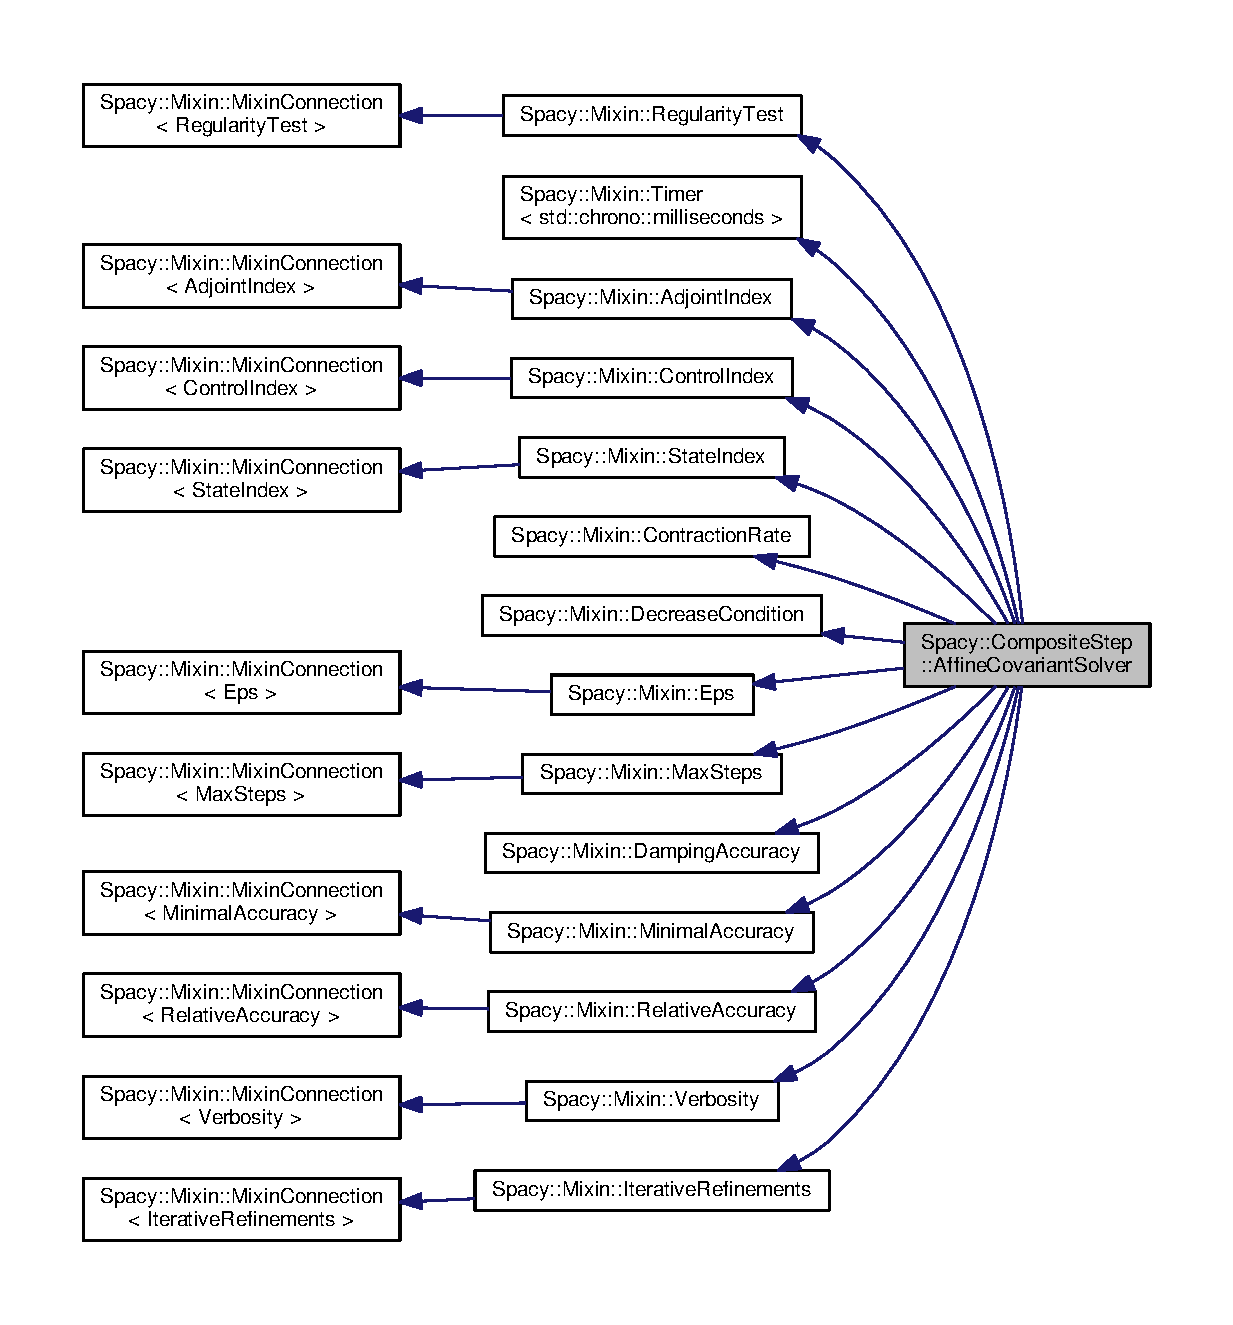
\includegraphics[width=350pt]{classSpacy_1_1CompositeStep_1_1AffineCovariantSolver__inherit__graph}
\end{center}
\end{figure}


Collaboration diagram for Spacy\+:\+:Composite\+Step\+:\+:Affine\+Covariant\+Solver\+:\nopagebreak
\begin{figure}[H]
\begin{center}
\leavevmode
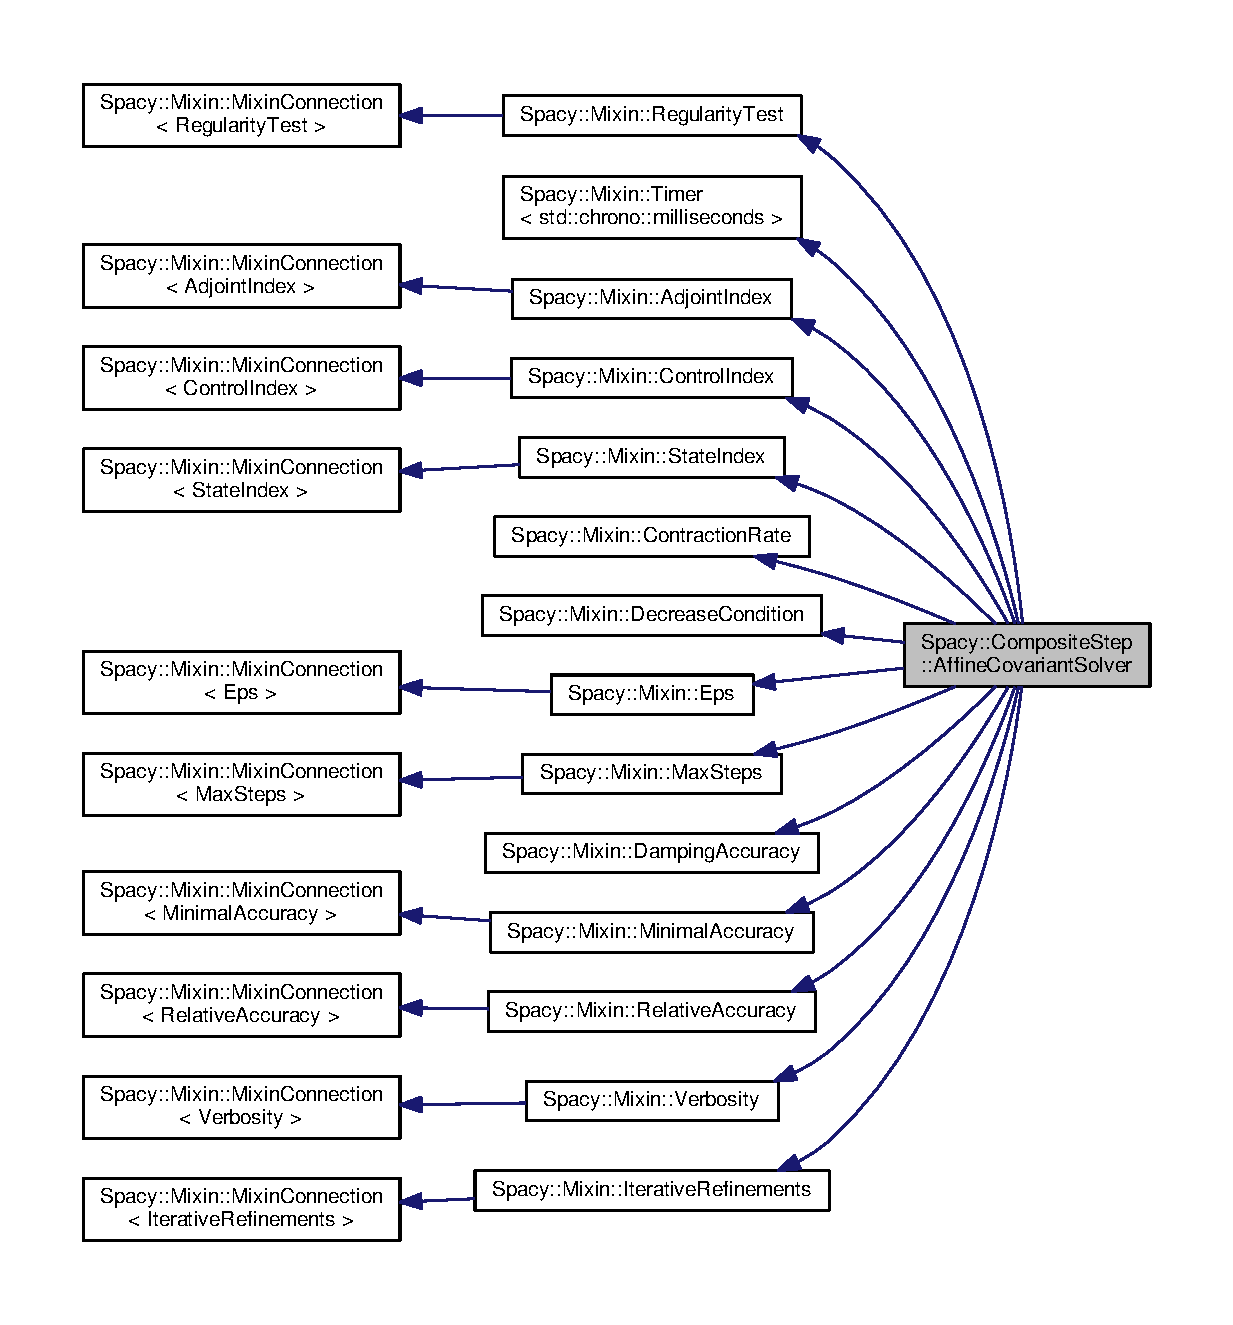
\includegraphics[width=350pt]{classSpacy_1_1CompositeStep_1_1AffineCovariantSolver__coll__graph}
\end{center}
\end{figure}
\subsection*{Public Member Functions}
\begin{DoxyCompactItemize}
\item 
\hyperlink{classSpacy_1_1CompositeStep_1_1AffineCovariantSolver_af81f7894dc2b7ee3533ab67d82195751_af81f7894dc2b7ee3533ab67d82195751}{Affine\+Covariant\+Solver} (\hyperlink{group__SpacyGroup_gaf5b89e117806134b06a1ce4629fb2b65_gaf5b89e117806134b06a1ce4629fb2b65}{C2\+Functional} N, \hyperlink{group__SpacyGroup_gaf5b89e117806134b06a1ce4629fb2b65_gaf5b89e117806134b06a1ce4629fb2b65}{C2\+Functional} L, \hyperlink{classSpacy_1_1VectorSpace}{Vector\+Space} \&domain)
\begin{DoxyCompactList}\small\item\em Constructor. \end{DoxyCompactList}\item 
\hypertarget{classSpacy_1_1CompositeStep_1_1AffineCovariantSolver_a010068164773b4062ec122b253a8226c}{}\hyperlink{classSpacy_1_1Vector}{Vector} \hyperlink{classSpacy_1_1CompositeStep_1_1AffineCovariantSolver_a010068164773b4062ec122b253a8226c}{operator()} ()\label{classSpacy_1_1CompositeStep_1_1AffineCovariantSolver_a010068164773b4062ec122b253a8226c}

\begin{DoxyCompactList}\small\item\em Compute solution. \end{DoxyCompactList}\item 
\hyperlink{classSpacy_1_1Vector}{Vector} \hyperlink{classSpacy_1_1CompositeStep_1_1AffineCovariantSolver_ae08612c2a1ca88d9a3746766bd5c1035_ae08612c2a1ca88d9a3746766bd5c1035}{operator()} (const \hyperlink{classSpacy_1_1Vector}{Vector} \&x0)
\begin{DoxyCompactList}\small\item\em Compute solution. \end{DoxyCompactList}\item 
void \hyperlink{classSpacy_1_1Mixin_1_1RegularityTest_a051394f2ffb0abd9a26ab7a64c590eee_a051394f2ffb0abd9a26ab7a64c590eee}{set\+Lower\+Bound} (\hyperlink{classSpacy_1_1Real}{Real} \hyperlink{classSpacy_1_1Mixin_1_1RegularityTest_a8a807e4449e6b6b64e7e81834d331597_a8a807e4449e6b6b64e7e81834d331597}{lower\+Bound})
\begin{DoxyCompactList}\small\item\em Set lower bound of regularity test for termination criteria. \end{DoxyCompactList}\item 
\hyperlink{classSpacy_1_1Real}{Real} \hyperlink{classSpacy_1_1Mixin_1_1RegularityTest_a8a807e4449e6b6b64e7e81834d331597_a8a807e4449e6b6b64e7e81834d331597}{lower\+Bound} () const noexcept
\begin{DoxyCompactList}\small\item\em Access lower bound. \end{DoxyCompactList}\item 
bool \hyperlink{classSpacy_1_1Mixin_1_1RegularityTest_afe2fd3259850b874a85779d4f562e7f6_afe2fd3259850b874a85779d4f562e7f6}{regularity\+Test\+Passed} (\hyperlink{classSpacy_1_1Real}{Real} nu) const noexcept
\begin{DoxyCompactList}\small\item\em Apply regularity test. \end{DoxyCompactList}\item 
bool \hyperlink{classSpacy_1_1Mixin_1_1RegularityTest_a26217e26765bb6f938224ea76612c8c0_a26217e26765bb6f938224ea76612c8c0}{regularity\+Test\+Failed} (\hyperlink{classSpacy_1_1Real}{Real} nu) const noexcept
\begin{DoxyCompactList}\small\item\em Apply regularity test. \end{DoxyCompactList}\item 
void \hyperlink{classSpacy_1_1Mixin_1_1RegularityTest_aeb6598687d622ef266d1ed515d2b42bf_aeb6598687d622ef266d1ed515d2b42bf}{attach\+Regularity\+Test} (\hyperlink{classSpacy_1_1Mixin_1_1RegularityTest_ae2887fec9a5bdd42239b3df6750bf2e9_ae2887fec9a5bdd42239b3df6750bf2e9}{Regularity\+Test} \&other)
\begin{DoxyCompactList}\small\item\em Attach \hyperlink{classSpacy_1_1Mixin_1_1RegularityTest}{Regularity\+Test}. \end{DoxyCompactList}\item 
\hypertarget{classSpacy_1_1Mixin_1_1RegularityTest_a289d6422bd82864d661bdbcfc7dc321e}{}void \hyperlink{classSpacy_1_1Mixin_1_1RegularityTest_a289d6422bd82864d661bdbcfc7dc321e}{detach\+Regularity\+Test} (\hyperlink{classSpacy_1_1Mixin_1_1RegularityTest_ae2887fec9a5bdd42239b3df6750bf2e9_ae2887fec9a5bdd42239b3df6750bf2e9}{Regularity\+Test} \&other)\label{classSpacy_1_1Mixin_1_1RegularityTest_a289d6422bd82864d661bdbcfc7dc321e}

\begin{DoxyCompactList}\small\item\em Detach \hyperlink{classSpacy_1_1Mixin_1_1Eps}{Eps} before it gets deleted. \end{DoxyCompactList}\item 
\hypertarget{classSpacy_1_1Mixin_1_1RegularityTest_ae3bfc55bec9fe3068adffb6d24b3b964}{}void \hyperlink{classSpacy_1_1Mixin_1_1RegularityTest_ae3bfc55bec9fe3068adffb6d24b3b964}{update} (Mixin\+Connection$<$ \hyperlink{classSpacy_1_1Mixin_1_1RegularityTest_ae2887fec9a5bdd42239b3df6750bf2e9_ae2887fec9a5bdd42239b3df6750bf2e9}{Regularity\+Test} $>$ $\ast$changed\+Subject)\label{classSpacy_1_1Mixin_1_1RegularityTest_ae3bfc55bec9fe3068adffb6d24b3b964}

\begin{DoxyCompactList}\small\item\em update function for observer pattern. \end{DoxyCompactList}\item 
\hypertarget{classSpacy_1_1Mixin_1_1Timer_acf3c292b6d482c7c4ded5f961be4bc4b}{}void \hyperlink{classSpacy_1_1Mixin_1_1Timer_acf3c292b6d482c7c4ded5f961be4bc4b}{start\+Timer} () const\label{classSpacy_1_1Mixin_1_1Timer_acf3c292b6d482c7c4ded5f961be4bc4b}

\begin{DoxyCompactList}\small\item\em Start timer. \end{DoxyCompactList}\item 
std\+::chrono\+::high\+\_\+resolution\+\_\+clock\+::rep \hyperlink{classSpacy_1_1Mixin_1_1Timer_ab27a20d8e1e9bc90ea56cb18ff752798_ab27a20d8e1e9bc90ea56cb18ff752798}{elapsed\+Time} () const
\begin{DoxyCompactList}\small\item\em Get elapsed time. \end{DoxyCompactList}\item 
\hypertarget{classSpacy_1_1Mixin_1_1Timer_a3b79b35213702118d0823f6040d5a315}{}void \hyperlink{classSpacy_1_1Mixin_1_1Timer_a3b79b35213702118d0823f6040d5a315}{print\+Elapsed\+Time} () const\label{classSpacy_1_1Mixin_1_1Timer_a3b79b35213702118d0823f6040d5a315}

\begin{DoxyCompactList}\small\item\em Print elapsed time to std\+::cout. \end{DoxyCompactList}\item 
void \hyperlink{classSpacy_1_1Mixin_1_1AdjointIndex_a30d4dd8b61175144c84c5bbf964528d7_a30d4dd8b61175144c84c5bbf964528d7}{set\+Adjoint\+Index} (unsigned index)
\begin{DoxyCompactList}\small\item\em Set index of the adjoint variable. \end{DoxyCompactList}\item 
double \hyperlink{classSpacy_1_1Mixin_1_1AdjointIndex_afd5c0f6bd67d20c88ea65b7f8fe4ab45_afd5c0f6bd67d20c88ea65b7f8fe4ab45}{adjoint\+Index} () const noexcept
\begin{DoxyCompactList}\small\item\em Access index of the adjoint variable. \end{DoxyCompactList}\item 
void \hyperlink{classSpacy_1_1Mixin_1_1AdjointIndex_a6ac8bb62f7d40cdf7aee68539026a647_a6ac8bb62f7d40cdf7aee68539026a647}{attach\+Adjoint\+Index} (\hyperlink{classSpacy_1_1Mixin_1_1AdjointIndex_a18dca16025bfc2af67da2eee34be9699_a18dca16025bfc2af67da2eee34be9699}{Adjoint\+Index} \&other)
\begin{DoxyCompactList}\small\item\em Attach adjoint index. \end{DoxyCompactList}\item 
\hypertarget{classSpacy_1_1Mixin_1_1AdjointIndex_af07504e2900cd83446469b4bb0ce0a4a}{}void \hyperlink{classSpacy_1_1Mixin_1_1AdjointIndex_af07504e2900cd83446469b4bb0ce0a4a}{detach\+Adjoint\+Index} (\hyperlink{classSpacy_1_1Mixin_1_1AdjointIndex_a18dca16025bfc2af67da2eee34be9699_a18dca16025bfc2af67da2eee34be9699}{Adjoint\+Index} \&other)\label{classSpacy_1_1Mixin_1_1AdjointIndex_af07504e2900cd83446469b4bb0ce0a4a}

\begin{DoxyCompactList}\small\item\em Detach verbosity before it gets deleted. \end{DoxyCompactList}\item 
\hypertarget{classSpacy_1_1Mixin_1_1AdjointIndex_ad91ccf68601950801cd062afee8a8cf2}{}void \hyperlink{classSpacy_1_1Mixin_1_1AdjointIndex_ad91ccf68601950801cd062afee8a8cf2}{update} (\hyperlink{classSpacy_1_1Mixin_1_1AdjointIndex_a18dca16025bfc2af67da2eee34be9699_a18dca16025bfc2af67da2eee34be9699}{Adjoint\+Index} $\ast$changed\+Subject)\label{classSpacy_1_1Mixin_1_1AdjointIndex_ad91ccf68601950801cd062afee8a8cf2}

\begin{DoxyCompactList}\small\item\em update function for observer pattern. \end{DoxyCompactList}\item 
void \hyperlink{classSpacy_1_1Mixin_1_1ControlIndex_a4e6c305c148d81f15638fc214f60ed00_a4e6c305c148d81f15638fc214f60ed00}{set\+Control\+Index} (unsigned index)
\begin{DoxyCompactList}\small\item\em Set index of the control variable. \end{DoxyCompactList}\item 
double \hyperlink{classSpacy_1_1Mixin_1_1ControlIndex_a04fd74c67e320942ff6513fe0a741913_a04fd74c67e320942ff6513fe0a741913}{control\+Index} () const noexcept
\begin{DoxyCompactList}\small\item\em Get index of control variable. \end{DoxyCompactList}\item 
void \hyperlink{classSpacy_1_1Mixin_1_1ControlIndex_a31b734645d51290cb4db6798018ab232_a31b734645d51290cb4db6798018ab232}{attach\+Control\+Index} (\hyperlink{classSpacy_1_1Mixin_1_1ControlIndex_afa09ff1cc2b7476e8b6e7e26e71cd775_afa09ff1cc2b7476e8b6e7e26e71cd775}{Control\+Index} \&other)
\begin{DoxyCompactList}\small\item\em Attach control index. \end{DoxyCompactList}\item 
\hypertarget{classSpacy_1_1Mixin_1_1ControlIndex_a3b39990dd9cf45d046966fb026c4a9ee}{}void \hyperlink{classSpacy_1_1Mixin_1_1ControlIndex_a3b39990dd9cf45d046966fb026c4a9ee}{detach\+Control\+Index} (\hyperlink{classSpacy_1_1Mixin_1_1ControlIndex_afa09ff1cc2b7476e8b6e7e26e71cd775_afa09ff1cc2b7476e8b6e7e26e71cd775}{Control\+Index} \&other)\label{classSpacy_1_1Mixin_1_1ControlIndex_a3b39990dd9cf45d046966fb026c4a9ee}

\begin{DoxyCompactList}\small\item\em Detach verbosity before it gets deleted. \end{DoxyCompactList}\item 
\hypertarget{classSpacy_1_1Mixin_1_1ControlIndex_aa534a05629e88a5cc479f161139cf3f7}{}void \hyperlink{classSpacy_1_1Mixin_1_1ControlIndex_aa534a05629e88a5cc479f161139cf3f7}{update} (\hyperlink{classSpacy_1_1Mixin_1_1ControlIndex_afa09ff1cc2b7476e8b6e7e26e71cd775_afa09ff1cc2b7476e8b6e7e26e71cd775}{Control\+Index} $\ast$changed\+Subject)\label{classSpacy_1_1Mixin_1_1ControlIndex_aa534a05629e88a5cc479f161139cf3f7}

\begin{DoxyCompactList}\small\item\em update function for observer pattern. \end{DoxyCompactList}\item 
void \hyperlink{classSpacy_1_1Mixin_1_1StateIndex_a7547d4239437b878cde8a60a95b0b319_a7547d4239437b878cde8a60a95b0b319}{set\+State\+Index} (unsigned index)
\begin{DoxyCompactList}\small\item\em Set index of state variable. \end{DoxyCompactList}\item 
double \hyperlink{classSpacy_1_1Mixin_1_1StateIndex_a8f6d3b42f3ffe6698ed9915355d22baa_a8f6d3b42f3ffe6698ed9915355d22baa}{state\+Index} () const noexcept
\begin{DoxyCompactList}\small\item\em Access index of state variable. \end{DoxyCompactList}\item 
void \hyperlink{classSpacy_1_1Mixin_1_1StateIndex_af307c6e75fe7839a3f74ea400b9aea4a_af307c6e75fe7839a3f74ea400b9aea4a}{attach\+State\+Index} (\hyperlink{classSpacy_1_1Mixin_1_1StateIndex_a0dfcecf87c0982d6c4d8859661aad1fa_a0dfcecf87c0982d6c4d8859661aad1fa}{State\+Index} \&other)
\begin{DoxyCompactList}\small\item\em Attach state index. \end{DoxyCompactList}\item 
\hypertarget{classSpacy_1_1Mixin_1_1StateIndex_ac193f8197435643fb7f509756607e464}{}void \hyperlink{classSpacy_1_1Mixin_1_1StateIndex_ac193f8197435643fb7f509756607e464}{detach\+State\+Index} (\hyperlink{classSpacy_1_1Mixin_1_1StateIndex_a0dfcecf87c0982d6c4d8859661aad1fa_a0dfcecf87c0982d6c4d8859661aad1fa}{State\+Index} \&other)\label{classSpacy_1_1Mixin_1_1StateIndex_ac193f8197435643fb7f509756607e464}

\begin{DoxyCompactList}\small\item\em Detach verbosity before it gets deleted. \end{DoxyCompactList}\item 
\hypertarget{classSpacy_1_1Mixin_1_1StateIndex_a632299c8de748ea73d1fcbbb4d8f734a}{}void \hyperlink{classSpacy_1_1Mixin_1_1StateIndex_a632299c8de748ea73d1fcbbb4d8f734a}{update} (\hyperlink{classSpacy_1_1Mixin_1_1StateIndex_a0dfcecf87c0982d6c4d8859661aad1fa_a0dfcecf87c0982d6c4d8859661aad1fa}{State\+Index} $\ast$changed\+Subject)\label{classSpacy_1_1Mixin_1_1StateIndex_a632299c8de748ea73d1fcbbb4d8f734a}

\begin{DoxyCompactList}\small\item\em update function for observer pattern. \end{DoxyCompactList}\item 
void \hyperlink{classSpacy_1_1Mixin_1_1ContractionRate_ab9215981f0454bd5d641abad582e64e5_ab9215981f0454bd5d641abad582e64e5}{set\+Contraction} (\hyperlink{classSpacy_1_1Real}{Real} \hyperlink{classSpacy_1_1Mixin_1_1ContractionRate_a6c5e653393be91e468364733702e5334_a6c5e653393be91e468364733702e5334}{contraction}) noexcept
\begin{DoxyCompactList}\small\item\em Set contraction rate. \end{DoxyCompactList}\item 
void \hyperlink{classSpacy_1_1Mixin_1_1ContractionRate_a26eaa6344b5b2191931a9fd87ed96f39_a26eaa6344b5b2191931a9fd87ed96f39}{set\+Desired\+Contraction} (\hyperlink{classSpacy_1_1Real}{Real} \hyperlink{classSpacy_1_1Mixin_1_1ContractionRate_aaefb97e44b51fb6c8017eb2b40659d64_aaefb97e44b51fb6c8017eb2b40659d64}{desired\+Contraction}) noexcept
\begin{DoxyCompactList}\small\item\em Set desired contraction rate. \end{DoxyCompactList}\item 
void \hyperlink{classSpacy_1_1Mixin_1_1ContractionRate_ac6e47c0ab683643fea7490703f02632d_ac6e47c0ab683643fea7490703f02632d}{set\+Relaxed\+Desired\+Contraction} (\hyperlink{classSpacy_1_1Real}{Real} \hyperlink{classSpacy_1_1Mixin_1_1ContractionRate_a569e3e3766394ccc46a13bd6ca122394_a569e3e3766394ccc46a13bd6ca122394}{relaxed\+Desired\+Contraction}) noexcept
\begin{DoxyCompactList}\small\item\em Set relaxed desired contraction rate. \end{DoxyCompactList}\item 
void \hyperlink{classSpacy_1_1Mixin_1_1ContractionRate_acc99ba536cd9a027baa50a1412d9d216_acc99ba536cd9a027baa50a1412d9d216}{set\+Maximal\+Contraction} (\hyperlink{classSpacy_1_1Real}{Real} \hyperlink{classSpacy_1_1Mixin_1_1ContractionRate_adea1388b1e492db1392f67cbe7e89302_adea1388b1e492db1392f67cbe7e89302}{maximal\+Contraction}) noexcept
\begin{DoxyCompactList}\small\item\em Set maximal contraction rate. \end{DoxyCompactList}\item 
\hyperlink{classSpacy_1_1Real}{Real} \hyperlink{classSpacy_1_1Mixin_1_1ContractionRate_a6c5e653393be91e468364733702e5334_a6c5e653393be91e468364733702e5334}{contraction} () const noexcept
\begin{DoxyCompactList}\small\item\em Access contraction rate. \end{DoxyCompactList}\item 
\hyperlink{classSpacy_1_1Real}{Real} \hyperlink{classSpacy_1_1Mixin_1_1ContractionRate_aaefb97e44b51fb6c8017eb2b40659d64_aaefb97e44b51fb6c8017eb2b40659d64}{desired\+Contraction} () const noexcept
\begin{DoxyCompactList}\small\item\em Access desired contraction rate. \end{DoxyCompactList}\item 
\hyperlink{classSpacy_1_1Real}{Real} \hyperlink{classSpacy_1_1Mixin_1_1ContractionRate_a569e3e3766394ccc46a13bd6ca122394_a569e3e3766394ccc46a13bd6ca122394}{relaxed\+Desired\+Contraction} () const noexcept
\begin{DoxyCompactList}\small\item\em Get relaxed desired contraction rate. \end{DoxyCompactList}\item 
\hyperlink{classSpacy_1_1Real}{Real} \hyperlink{classSpacy_1_1Mixin_1_1ContractionRate_adea1388b1e492db1392f67cbe7e89302_adea1388b1e492db1392f67cbe7e89302}{maximal\+Contraction} () const noexcept
\begin{DoxyCompactList}\small\item\em Get desired contraction rate. \end{DoxyCompactList}\item 
bool \hyperlink{classSpacy_1_1Mixin_1_1ContractionRate_a7dd3c5eb5a7d14d8269207e3d1203aec_a7dd3c5eb5a7d14d8269207e3d1203aec}{admissible\+Contraction} () const noexcept
\begin{DoxyCompactList}\small\item\em Check if contraction is admissible. \end{DoxyCompactList}\item 
void \hyperlink{classSpacy_1_1Mixin_1_1DecreaseCondition_aabc5e2473edace0c87da7fbd9fa0ae61_aabc5e2473edace0c87da7fbd9fa0ae61}{set\+Minimal\+Decrease} (\hyperlink{classSpacy_1_1Real}{Real} decrease) noexcept
\begin{DoxyCompactList}\small\item\em Set required minimal decrease. \end{DoxyCompactList}\item 
\hyperlink{classSpacy_1_1Real}{Real} \hyperlink{classSpacy_1_1Mixin_1_1DecreaseCondition_aeeda8b1d9f177fe5dd532e42de09ab44_aeeda8b1d9f177fe5dd532e42de09ab44}{minimal\+Decrease} () const noexcept
\begin{DoxyCompactList}\small\item\em Access minimal decrease. \end{DoxyCompactList}\item 
void \hyperlink{classSpacy_1_1Mixin_1_1DecreaseCondition_a86d6a8c8fc683c31572fd818a102a362_a86d6a8c8fc683c31572fd818a102a362}{set\+Relaxed\+Minimal\+Decrease} (\hyperlink{classSpacy_1_1Real}{Real} decrease) noexcept
\begin{DoxyCompactList}\small\item\em Set relaxed minimal decrease. \end{DoxyCompactList}\item 
bool \hyperlink{classSpacy_1_1Mixin_1_1DecreaseCondition_a69c0c90daf14fc40461876f71c49ffc2_a69c0c90daf14fc40461876f71c49ffc2}{acceptable\+Decrease} (\hyperlink{classSpacy_1_1Real}{Real} decrease) const noexcept
\begin{DoxyCompactList}\small\item\em Decide if measure relative decrease is acceptable. \end{DoxyCompactList}\item 
bool \hyperlink{classSpacy_1_1Mixin_1_1DecreaseCondition_a5ffb5bc008544db96d935a0ca34dcd24_a5ffb5bc008544db96d935a0ca34dcd24}{acceptable\+Relaxed\+Decrease} (\hyperlink{classSpacy_1_1Real}{Real} decrease) const noexcept
\begin{DoxyCompactList}\small\item\em Decide if measure relative decrease is acceptable with respect to the relaxed decrease condition. \end{DoxyCompactList}\item 
void \hyperlink{classSpacy_1_1Mixin_1_1Eps_a1bbfd62541610d5d80f2782ab77158e4_a1bbfd62541610d5d80f2782ab77158e4}{set\+Eps} (double \hyperlink{classSpacy_1_1Mixin_1_1Eps_a40e2ba8f3abd2b5370ef41238cfaaf8b_a40e2ba8f3abd2b5370ef41238cfaaf8b}{eps})
\begin{DoxyCompactList}\small\item\em Set maximal attainable accuracy $\varepsilon$. \end{DoxyCompactList}\item 
double \hyperlink{classSpacy_1_1Mixin_1_1Eps_a40e2ba8f3abd2b5370ef41238cfaaf8b_a40e2ba8f3abd2b5370ef41238cfaaf8b}{eps} () const noexcept
\begin{DoxyCompactList}\small\item\em Access maximal attainable accuracy. \end{DoxyCompactList}\item 
double \hyperlink{classSpacy_1_1Mixin_1_1Eps_a29e8c25dc3f1fdede57b8eb06f520fe1_a29e8c25dc3f1fdede57b8eb06f520fe1}{sqrt\+Eps} () const noexcept
\begin{DoxyCompactList}\small\item\em Access square root of maximal attainable accuracy. \end{DoxyCompactList}\item 
double \hyperlink{classSpacy_1_1Mixin_1_1Eps_a1879ebbf1b467cb4be36bcc63307018d_a1879ebbf1b467cb4be36bcc63307018d}{cbrt\+Eps} () const noexcept
\begin{DoxyCompactList}\small\item\em Get third root of maximal attainable accuracy. \end{DoxyCompactList}\item 
void \hyperlink{classSpacy_1_1Mixin_1_1Eps_af69cd3dee52e723302b21ca2a25f1192_af69cd3dee52e723302b21ca2a25f1192}{attach\+Eps} (\hyperlink{classSpacy_1_1Mixin_1_1Eps_a51dbe0b9cc950e0f3dfd34a481f08ae4_a51dbe0b9cc950e0f3dfd34a481f08ae4}{Eps} \&other)
\begin{DoxyCompactList}\small\item\em Attach \hyperlink{classSpacy_1_1Mixin_1_1Eps}{Eps}. \end{DoxyCompactList}\item 
\hypertarget{classSpacy_1_1Mixin_1_1Eps_ab49910e189cb86b6fd6f89b6f2af14cc}{}void \hyperlink{classSpacy_1_1Mixin_1_1Eps_ab49910e189cb86b6fd6f89b6f2af14cc}{detach\+Eps} (\hyperlink{classSpacy_1_1Mixin_1_1Eps_a51dbe0b9cc950e0f3dfd34a481f08ae4_a51dbe0b9cc950e0f3dfd34a481f08ae4}{Eps} \&other)\label{classSpacy_1_1Mixin_1_1Eps_ab49910e189cb86b6fd6f89b6f2af14cc}

\begin{DoxyCompactList}\small\item\em Detach \hyperlink{classSpacy_1_1Mixin_1_1Eps}{Eps} before it gets deleted. \end{DoxyCompactList}\item 
\hypertarget{classSpacy_1_1Mixin_1_1Eps_a151216968daef3da5f5cdc0b957ce01b}{}void \hyperlink{classSpacy_1_1Mixin_1_1Eps_a151216968daef3da5f5cdc0b957ce01b}{update} (\hyperlink{classSpacy_1_1Mixin_1_1Eps_a51dbe0b9cc950e0f3dfd34a481f08ae4_a51dbe0b9cc950e0f3dfd34a481f08ae4}{Eps} $\ast$changed\+Subject)\label{classSpacy_1_1Mixin_1_1Eps_a151216968daef3da5f5cdc0b957ce01b}

\begin{DoxyCompactList}\small\item\em update function for observer pattern. \end{DoxyCompactList}\item 
void \hyperlink{classSpacy_1_1Mixin_1_1MaxSteps_a72f0b7eb50c9a017b5f5e6c2ccf7dfd9_a72f0b7eb50c9a017b5f5e6c2ccf7dfd9}{set\+Max\+Steps} (unsigned \hyperlink{classSpacy_1_1Mixin_1_1MaxSteps_aaeb0b209c78e7b8dd9b268641ce11977_aaeb0b209c78e7b8dd9b268641ce11977}{max\+Steps})
\begin{DoxyCompactList}\small\item\em Set maximal number of steps/iterations for iterative solvers. \end{DoxyCompactList}\item 
unsigned \hyperlink{classSpacy_1_1Mixin_1_1MaxSteps_aaeb0b209c78e7b8dd9b268641ce11977_aaeb0b209c78e7b8dd9b268641ce11977}{max\+Steps} () const noexcept
\begin{DoxyCompactList}\small\item\em Get maximal number of steps/iterations for iterative solvers. \end{DoxyCompactList}\item 
void \hyperlink{classSpacy_1_1Mixin_1_1MaxSteps_a8b093369a1ce5a6323f3dc3c41a738e6_a8b093369a1ce5a6323f3dc3c41a738e6}{attach\+Max\+Steps} (\hyperlink{classSpacy_1_1Mixin_1_1MaxSteps_a8e5d8290884bdc760147862d5b9644dc_a8e5d8290884bdc760147862d5b9644dc}{Max\+Steps} \&other)
\begin{DoxyCompactList}\small\item\em Attach \hyperlink{classSpacy_1_1Mixin_1_1MaxSteps}{Max\+Steps}. \end{DoxyCompactList}\item 
\hypertarget{classSpacy_1_1Mixin_1_1MaxSteps_ac16eca4cd967aed1856f072b08f4aabd}{}void \hyperlink{classSpacy_1_1Mixin_1_1MaxSteps_ac16eca4cd967aed1856f072b08f4aabd}{detach\+Max\+Steps} (\hyperlink{classSpacy_1_1Mixin_1_1MaxSteps_a8e5d8290884bdc760147862d5b9644dc_a8e5d8290884bdc760147862d5b9644dc}{Max\+Steps} \&other)\label{classSpacy_1_1Mixin_1_1MaxSteps_ac16eca4cd967aed1856f072b08f4aabd}

\begin{DoxyCompactList}\small\item\em Detach \hyperlink{classSpacy_1_1Mixin_1_1Eps}{Eps} before it gets deleted. \end{DoxyCompactList}\item 
\hypertarget{classSpacy_1_1Mixin_1_1MaxSteps_a8e0f4d29b15dff17d4503788a9e2e081}{}void \hyperlink{classSpacy_1_1Mixin_1_1MaxSteps_a8e0f4d29b15dff17d4503788a9e2e081}{update} (\hyperlink{classSpacy_1_1Mixin_1_1MaxSteps_a8e5d8290884bdc760147862d5b9644dc_a8e5d8290884bdc760147862d5b9644dc}{Max\+Steps} $\ast$changed\+Subject)\label{classSpacy_1_1Mixin_1_1MaxSteps_a8e0f4d29b15dff17d4503788a9e2e081}

\begin{DoxyCompactList}\small\item\em update function for observer pattern. \end{DoxyCompactList}\item 
void \hyperlink{classSpacy_1_1Mixin_1_1DampingAccuracy_af934aaf17595b7029d9a8ecec2561599_af934aaf17595b7029d9a8ecec2561599}{set\+Damping\+Accuracy} (double accuracy) noexcept
\begin{DoxyCompactList}\small\item\em Set accuracy for damping factors. \end{DoxyCompactList}\item 
double \hyperlink{classSpacy_1_1Mixin_1_1DampingAccuracy_a070c4c1b64c4392c6b21478bcf4c4a75_a070c4c1b64c4392c6b21478bcf4c4a75}{damping\+Accuracy} () const noexcept
\begin{DoxyCompactList}\small\item\em Access accuracy for damping factors. \end{DoxyCompactList}\item 
void \hyperlink{classSpacy_1_1Mixin_1_1MinimalAccuracy_a34d3d3320bba45d5c6c06b65e2cc808b_a34d3d3320bba45d5c6c06b65e2cc808b}{set\+Minimal\+Accuracy} (double accuracy)
\begin{DoxyCompactList}\small\item\em Set minimal accuracy. \end{DoxyCompactList}\item 
double \hyperlink{classSpacy_1_1Mixin_1_1MinimalAccuracy_ab9e4346b7070ce179593fc38d556705b_ab9e4346b7070ce179593fc38d556705b}{minimal\+Accuracy} () const noexcept
\begin{DoxyCompactList}\small\item\em Access minimal accuracy. \end{DoxyCompactList}\item 
void \hyperlink{classSpacy_1_1Mixin_1_1MinimalAccuracy_a0b2039bf970afdb0ede9999d6567f49b_a0b2039bf970afdb0ede9999d6567f49b}{attach\+Minimal\+Accuracy} (\hyperlink{classSpacy_1_1Mixin_1_1MinimalAccuracy_a9dc80f566f27efbd48c43c7f7c0961c2_a9dc80f566f27efbd48c43c7f7c0961c2}{Minimal\+Accuracy} \&other)
\begin{DoxyCompactList}\small\item\em Attach \hyperlink{classSpacy_1_1Mixin_1_1MinimalAccuracy}{Minimal\+Accuracy}. \end{DoxyCompactList}\item 
\hypertarget{classSpacy_1_1Mixin_1_1MinimalAccuracy_adb422b74482cdef5ffaff816da86b18d}{}void \hyperlink{classSpacy_1_1Mixin_1_1MinimalAccuracy_adb422b74482cdef5ffaff816da86b18d}{detach\+Minimal\+Accuracy} (\hyperlink{classSpacy_1_1Mixin_1_1MinimalAccuracy_a9dc80f566f27efbd48c43c7f7c0961c2_a9dc80f566f27efbd48c43c7f7c0961c2}{Minimal\+Accuracy} \&other)\label{classSpacy_1_1Mixin_1_1MinimalAccuracy_adb422b74482cdef5ffaff816da86b18d}

\begin{DoxyCompactList}\small\item\em Detach \hyperlink{classSpacy_1_1Mixin_1_1RelativeAccuracy}{Relative\+Accuracy} before it gets deleted. \end{DoxyCompactList}\item 
\hypertarget{classSpacy_1_1Mixin_1_1MinimalAccuracy_a98dc7eb03f50165f6f2e0df17c2b7d44}{}void \hyperlink{classSpacy_1_1Mixin_1_1MinimalAccuracy_a98dc7eb03f50165f6f2e0df17c2b7d44}{update} (\hyperlink{classSpacy_1_1Mixin_1_1MinimalAccuracy_a9dc80f566f27efbd48c43c7f7c0961c2_a9dc80f566f27efbd48c43c7f7c0961c2}{Minimal\+Accuracy} $\ast$changed\+Subject)\label{classSpacy_1_1Mixin_1_1MinimalAccuracy_a98dc7eb03f50165f6f2e0df17c2b7d44}

\begin{DoxyCompactList}\small\item\em update function for observer pattern. \end{DoxyCompactList}\item 
void \hyperlink{classSpacy_1_1Mixin_1_1RelativeAccuracy_aee88b71e80aca446a179f1310408a1e3_aee88b71e80aca446a179f1310408a1e3}{set\+Relative\+Accuracy} (double accuracy)
\begin{DoxyCompactList}\small\item\em Set relative accuracy. \end{DoxyCompactList}\item 
double \hyperlink{classSpacy_1_1Mixin_1_1RelativeAccuracy_a1da618cf9265c2edae354524df4a7f8a_a1da618cf9265c2edae354524df4a7f8a}{relative\+Accuracy} () const noexcept
\begin{DoxyCompactList}\small\item\em Access relative accuracy. \end{DoxyCompactList}\item 
void \hyperlink{classSpacy_1_1Mixin_1_1RelativeAccuracy_ae299bb5419df551cc93c6397e5b1b58b_ae299bb5419df551cc93c6397e5b1b58b}{attach\+Relative\+Accuracy} (\hyperlink{classSpacy_1_1Mixin_1_1RelativeAccuracy_ad843319a8782b47291fa31334e8bbd2a_ad843319a8782b47291fa31334e8bbd2a}{Relative\+Accuracy} \&other)
\begin{DoxyCompactList}\small\item\em Attach \hyperlink{classSpacy_1_1Mixin_1_1RelativeAccuracy}{Relative\+Accuracy}. \end{DoxyCompactList}\item 
\hypertarget{classSpacy_1_1Mixin_1_1RelativeAccuracy_a2636cde30aab8415e19e25fc12489e57}{}void \hyperlink{classSpacy_1_1Mixin_1_1RelativeAccuracy_a2636cde30aab8415e19e25fc12489e57}{detach\+Relative\+Accuracy} (\hyperlink{classSpacy_1_1Mixin_1_1RelativeAccuracy_ad843319a8782b47291fa31334e8bbd2a_ad843319a8782b47291fa31334e8bbd2a}{Relative\+Accuracy} \&other)\label{classSpacy_1_1Mixin_1_1RelativeAccuracy_a2636cde30aab8415e19e25fc12489e57}

\begin{DoxyCompactList}\small\item\em Detach \hyperlink{classSpacy_1_1Mixin_1_1RelativeAccuracy}{Relative\+Accuracy} before it gets deleted. \end{DoxyCompactList}\item 
\hypertarget{classSpacy_1_1Mixin_1_1RelativeAccuracy_acf0b58224d9a2879d05b5d2947f37527}{}void \hyperlink{classSpacy_1_1Mixin_1_1RelativeAccuracy_acf0b58224d9a2879d05b5d2947f37527}{update} (\hyperlink{classSpacy_1_1Mixin_1_1RelativeAccuracy_ad843319a8782b47291fa31334e8bbd2a_ad843319a8782b47291fa31334e8bbd2a}{Relative\+Accuracy} $\ast$changed\+Subject)\label{classSpacy_1_1Mixin_1_1RelativeAccuracy_acf0b58224d9a2879d05b5d2947f37527}

\begin{DoxyCompactList}\small\item\em update function for observer pattern. \end{DoxyCompactList}\item 
void \hyperlink{classSpacy_1_1Mixin_1_1Verbosity_a0365d293ab27e27da9496c668020aefb_a0365d293ab27e27da9496c668020aefb}{set\+Verbosity} (bool \hyperlink{classSpacy_1_1Mixin_1_1Verbosity_ad367a7328578546938fd2a7e52ab3793_ad367a7328578546938fd2a7e52ab3793}{verbose})
\begin{DoxyCompactList}\small\item\em Enable/disable verbosity. \end{DoxyCompactList}\item 
bool \hyperlink{classSpacy_1_1Mixin_1_1Verbosity_ad367a7328578546938fd2a7e52ab3793_ad367a7328578546938fd2a7e52ab3793}{verbose} () const noexcept
\begin{DoxyCompactList}\small\item\em Check if verbosity is turned on. \end{DoxyCompactList}\item 
void \hyperlink{classSpacy_1_1Mixin_1_1Verbosity_af84a4b3c933f252a5840ab63d4a38325_af84a4b3c933f252a5840ab63d4a38325}{set\+Verbosity\+Level} (unsigned level) noexcept
\begin{DoxyCompactList}\small\item\em Set verbosity level. \end{DoxyCompactList}\item 
unsigned \hyperlink{classSpacy_1_1Mixin_1_1Verbosity_a2131f495d276c95d2d6534a6dfce6f9f_a2131f495d276c95d2d6534a6dfce6f9f}{verbosity\+Level} () const noexcept
\begin{DoxyCompactList}\small\item\em Access verbosity level. \end{DoxyCompactList}\item 
void \hyperlink{classSpacy_1_1Mixin_1_1Verbosity_a69fe3a0107ec34780f1d74b46b1b53b5_a69fe3a0107ec34780f1d74b46b1b53b5}{attach\+Verbosity} (\hyperlink{classSpacy_1_1Mixin_1_1Verbosity_aefe2f237b0456c4bced001fbfa75f92e_aefe2f237b0456c4bced001fbfa75f92e}{Verbosity} \&other)
\begin{DoxyCompactList}\small\item\em Attach verbosity. \end{DoxyCompactList}\item 
\hypertarget{classSpacy_1_1Mixin_1_1Verbosity_a86ec8efe73d1ce2768bf645f0627b325}{}void \hyperlink{classSpacy_1_1Mixin_1_1Verbosity_a86ec8efe73d1ce2768bf645f0627b325}{detach\+Verbosity} (\hyperlink{classSpacy_1_1Mixin_1_1Verbosity_aefe2f237b0456c4bced001fbfa75f92e_aefe2f237b0456c4bced001fbfa75f92e}{Verbosity} \&other)\label{classSpacy_1_1Mixin_1_1Verbosity_a86ec8efe73d1ce2768bf645f0627b325}

\begin{DoxyCompactList}\small\item\em Detach verbosity before it gets deleted. \end{DoxyCompactList}\item 
\hypertarget{classSpacy_1_1Mixin_1_1Verbosity_a8cff860c587fcda2cdc86ba744302b33}{}void \hyperlink{classSpacy_1_1Mixin_1_1Verbosity_a8cff860c587fcda2cdc86ba744302b33}{update} (\hyperlink{classSpacy_1_1Mixin_1_1Verbosity_aefe2f237b0456c4bced001fbfa75f92e_aefe2f237b0456c4bced001fbfa75f92e}{Verbosity} $\ast$changed\+Subject)\label{classSpacy_1_1Mixin_1_1Verbosity_a8cff860c587fcda2cdc86ba744302b33}

\begin{DoxyCompactList}\small\item\em update function for observer pattern. \end{DoxyCompactList}\item 
void \hyperlink{classSpacy_1_1Mixin_1_1IterativeRefinements_afd8815d6932a99b1700f54162d9f633e_afd8815d6932a99b1700f54162d9f633e}{set\+Iterative\+Refinements} (unsigned refinements)
\begin{DoxyCompactList}\small\item\em Set number of iterative refinements. \end{DoxyCompactList}\item 
unsigned \hyperlink{classSpacy_1_1Mixin_1_1IterativeRefinements_a560cd9428928c941765b71dd7c51ae3b_a560cd9428928c941765b71dd7c51ae3b}{iterative\+Refinements} () const 
\begin{DoxyCompactList}\small\item\em Access number of iterative refinements. \end{DoxyCompactList}\item 
void \hyperlink{classSpacy_1_1Mixin_1_1IterativeRefinements_ad2d1f161aa254d7511df897556e7613e_ad2d1f161aa254d7511df897556e7613e}{attach\+Iterative\+Refinements} (\hyperlink{classSpacy_1_1Mixin_1_1IterativeRefinements_a0cdc2228af8fe052680d24fc4bb7ed6a_a0cdc2228af8fe052680d24fc4bb7ed6a}{Iterative\+Refinements} \&other)
\begin{DoxyCompactList}\small\item\em Attach \hyperlink{classSpacy_1_1Mixin_1_1IterativeRefinements}{Iterative\+Refinements}. \end{DoxyCompactList}\item 
\hypertarget{classSpacy_1_1Mixin_1_1IterativeRefinements_aa3b4275d845ef9dabb3f5fefbed43112}{}void \hyperlink{classSpacy_1_1Mixin_1_1IterativeRefinements_aa3b4275d845ef9dabb3f5fefbed43112}{detach\+Iterative\+Refinements} (\hyperlink{classSpacy_1_1Mixin_1_1IterativeRefinements_a0cdc2228af8fe052680d24fc4bb7ed6a_a0cdc2228af8fe052680d24fc4bb7ed6a}{Iterative\+Refinements} \&other)\label{classSpacy_1_1Mixin_1_1IterativeRefinements_aa3b4275d845ef9dabb3f5fefbed43112}

\begin{DoxyCompactList}\small\item\em Detach \hyperlink{classSpacy_1_1Mixin_1_1Eps}{Eps} before it gets deleted. \end{DoxyCompactList}\item 
\hypertarget{classSpacy_1_1Mixin_1_1IterativeRefinements_adcb6062728331e48515a05f539628062}{}void \hyperlink{classSpacy_1_1Mixin_1_1IterativeRefinements_adcb6062728331e48515a05f539628062}{update} (\hyperlink{classSpacy_1_1Mixin_1_1IterativeRefinements_a0cdc2228af8fe052680d24fc4bb7ed6a_a0cdc2228af8fe052680d24fc4bb7ed6a}{Iterative\+Refinements} $\ast$changed\+Subject)\label{classSpacy_1_1Mixin_1_1IterativeRefinements_adcb6062728331e48515a05f539628062}

\begin{DoxyCompactList}\small\item\em update function for observer pattern. \end{DoxyCompactList}\end{DoxyCompactItemize}
\subsection*{Protected Member Functions}
\begin{DoxyCompactItemize}
\item 
\hypertarget{classSpacy_1_1Mixin_1_1MixinConnection_abb5520ee6b22dd993d78f142939a1ed4}{}void \hyperlink{classSpacy_1_1Mixin_1_1MixinConnection_abb5520ee6b22dd993d78f142939a1ed4}{attach} (\hyperlink{classSpacy_1_1Mixin_1_1RegularityTest_ae2887fec9a5bdd42239b3df6750bf2e9_ae2887fec9a5bdd42239b3df6750bf2e9}{Regularity\+Test} \&observer)\label{classSpacy_1_1Mixin_1_1MixinConnection_abb5520ee6b22dd993d78f142939a1ed4}

\begin{DoxyCompactList}\small\item\em Attach observer. \end{DoxyCompactList}\item 
\hypertarget{classSpacy_1_1Mixin_1_1MixinConnection_adda739590c487679c26f60e50aedb73f}{}void \hyperlink{classSpacy_1_1Mixin_1_1MixinConnection_adda739590c487679c26f60e50aedb73f}{detach} (\hyperlink{classSpacy_1_1Mixin_1_1RegularityTest_ae2887fec9a5bdd42239b3df6750bf2e9_ae2887fec9a5bdd42239b3df6750bf2e9}{Regularity\+Test} \&observer)\label{classSpacy_1_1Mixin_1_1MixinConnection_adda739590c487679c26f60e50aedb73f}

\begin{DoxyCompactList}\small\item\em Detach observer. \end{DoxyCompactList}\item 
\hypertarget{classSpacy_1_1Mixin_1_1MixinConnection_a1ddeaa78a3bb4a38c2cca36d1f99fe36}{}void \hyperlink{classSpacy_1_1Mixin_1_1MixinConnection_a1ddeaa78a3bb4a38c2cca36d1f99fe36}{notify} ()\label{classSpacy_1_1Mixin_1_1MixinConnection_a1ddeaa78a3bb4a38c2cca36d1f99fe36}

\begin{DoxyCompactList}\small\item\em Notify observers about changes. \end{DoxyCompactList}\item 
\hypertarget{classSpacy_1_1Mixin_1_1MixinConnection_abb5520ee6b22dd993d78f142939a1ed4}{}void \hyperlink{classSpacy_1_1Mixin_1_1MixinConnection_abb5520ee6b22dd993d78f142939a1ed4}{attach} (\hyperlink{classSpacy_1_1Mixin_1_1AdjointIndex_a18dca16025bfc2af67da2eee34be9699_a18dca16025bfc2af67da2eee34be9699}{Adjoint\+Index} \&observer)\label{classSpacy_1_1Mixin_1_1MixinConnection_abb5520ee6b22dd993d78f142939a1ed4}

\begin{DoxyCompactList}\small\item\em Attach observer. \end{DoxyCompactList}\item 
\hypertarget{classSpacy_1_1Mixin_1_1MixinConnection_adda739590c487679c26f60e50aedb73f}{}void \hyperlink{classSpacy_1_1Mixin_1_1MixinConnection_adda739590c487679c26f60e50aedb73f}{detach} (\hyperlink{classSpacy_1_1Mixin_1_1AdjointIndex_a18dca16025bfc2af67da2eee34be9699_a18dca16025bfc2af67da2eee34be9699}{Adjoint\+Index} \&observer)\label{classSpacy_1_1Mixin_1_1MixinConnection_adda739590c487679c26f60e50aedb73f}

\begin{DoxyCompactList}\small\item\em Detach observer. \end{DoxyCompactList}\item 
\hypertarget{classSpacy_1_1Mixin_1_1MixinConnection_a1ddeaa78a3bb4a38c2cca36d1f99fe36}{}void \hyperlink{classSpacy_1_1Mixin_1_1MixinConnection_a1ddeaa78a3bb4a38c2cca36d1f99fe36}{notify} ()\label{classSpacy_1_1Mixin_1_1MixinConnection_a1ddeaa78a3bb4a38c2cca36d1f99fe36}

\begin{DoxyCompactList}\small\item\em Notify observers about changes. \end{DoxyCompactList}\item 
\hypertarget{classSpacy_1_1Mixin_1_1MixinConnection_abb5520ee6b22dd993d78f142939a1ed4}{}void \hyperlink{classSpacy_1_1Mixin_1_1MixinConnection_abb5520ee6b22dd993d78f142939a1ed4}{attach} (\hyperlink{classSpacy_1_1Mixin_1_1ControlIndex_afa09ff1cc2b7476e8b6e7e26e71cd775_afa09ff1cc2b7476e8b6e7e26e71cd775}{Control\+Index} \&observer)\label{classSpacy_1_1Mixin_1_1MixinConnection_abb5520ee6b22dd993d78f142939a1ed4}

\begin{DoxyCompactList}\small\item\em Attach observer. \end{DoxyCompactList}\item 
\hypertarget{classSpacy_1_1Mixin_1_1MixinConnection_adda739590c487679c26f60e50aedb73f}{}void \hyperlink{classSpacy_1_1Mixin_1_1MixinConnection_adda739590c487679c26f60e50aedb73f}{detach} (\hyperlink{classSpacy_1_1Mixin_1_1ControlIndex_afa09ff1cc2b7476e8b6e7e26e71cd775_afa09ff1cc2b7476e8b6e7e26e71cd775}{Control\+Index} \&observer)\label{classSpacy_1_1Mixin_1_1MixinConnection_adda739590c487679c26f60e50aedb73f}

\begin{DoxyCompactList}\small\item\em Detach observer. \end{DoxyCompactList}\item 
\hypertarget{classSpacy_1_1Mixin_1_1MixinConnection_a1ddeaa78a3bb4a38c2cca36d1f99fe36}{}void \hyperlink{classSpacy_1_1Mixin_1_1MixinConnection_a1ddeaa78a3bb4a38c2cca36d1f99fe36}{notify} ()\label{classSpacy_1_1Mixin_1_1MixinConnection_a1ddeaa78a3bb4a38c2cca36d1f99fe36}

\begin{DoxyCompactList}\small\item\em Notify observers about changes. \end{DoxyCompactList}\item 
\hypertarget{classSpacy_1_1Mixin_1_1MixinConnection_abb5520ee6b22dd993d78f142939a1ed4}{}void \hyperlink{classSpacy_1_1Mixin_1_1MixinConnection_abb5520ee6b22dd993d78f142939a1ed4}{attach} (\hyperlink{classSpacy_1_1Mixin_1_1StateIndex_a0dfcecf87c0982d6c4d8859661aad1fa_a0dfcecf87c0982d6c4d8859661aad1fa}{State\+Index} \&observer)\label{classSpacy_1_1Mixin_1_1MixinConnection_abb5520ee6b22dd993d78f142939a1ed4}

\begin{DoxyCompactList}\small\item\em Attach observer. \end{DoxyCompactList}\item 
\hypertarget{classSpacy_1_1Mixin_1_1MixinConnection_adda739590c487679c26f60e50aedb73f}{}void \hyperlink{classSpacy_1_1Mixin_1_1MixinConnection_adda739590c487679c26f60e50aedb73f}{detach} (\hyperlink{classSpacy_1_1Mixin_1_1StateIndex_a0dfcecf87c0982d6c4d8859661aad1fa_a0dfcecf87c0982d6c4d8859661aad1fa}{State\+Index} \&observer)\label{classSpacy_1_1Mixin_1_1MixinConnection_adda739590c487679c26f60e50aedb73f}

\begin{DoxyCompactList}\small\item\em Detach observer. \end{DoxyCompactList}\item 
\hypertarget{classSpacy_1_1Mixin_1_1MixinConnection_a1ddeaa78a3bb4a38c2cca36d1f99fe36}{}void \hyperlink{classSpacy_1_1Mixin_1_1MixinConnection_a1ddeaa78a3bb4a38c2cca36d1f99fe36}{notify} ()\label{classSpacy_1_1Mixin_1_1MixinConnection_a1ddeaa78a3bb4a38c2cca36d1f99fe36}

\begin{DoxyCompactList}\small\item\em Notify observers about changes. \end{DoxyCompactList}\item 
\hypertarget{classSpacy_1_1Mixin_1_1MixinConnection_abb5520ee6b22dd993d78f142939a1ed4}{}void \hyperlink{classSpacy_1_1Mixin_1_1MixinConnection_abb5520ee6b22dd993d78f142939a1ed4}{attach} (\hyperlink{classSpacy_1_1Mixin_1_1Eps_a51dbe0b9cc950e0f3dfd34a481f08ae4_a51dbe0b9cc950e0f3dfd34a481f08ae4}{Eps} \&observer)\label{classSpacy_1_1Mixin_1_1MixinConnection_abb5520ee6b22dd993d78f142939a1ed4}

\begin{DoxyCompactList}\small\item\em Attach observer. \end{DoxyCompactList}\item 
\hypertarget{classSpacy_1_1Mixin_1_1MixinConnection_adda739590c487679c26f60e50aedb73f}{}void \hyperlink{classSpacy_1_1Mixin_1_1MixinConnection_adda739590c487679c26f60e50aedb73f}{detach} (\hyperlink{classSpacy_1_1Mixin_1_1Eps_a51dbe0b9cc950e0f3dfd34a481f08ae4_a51dbe0b9cc950e0f3dfd34a481f08ae4}{Eps} \&observer)\label{classSpacy_1_1Mixin_1_1MixinConnection_adda739590c487679c26f60e50aedb73f}

\begin{DoxyCompactList}\small\item\em Detach observer. \end{DoxyCompactList}\item 
\hypertarget{classSpacy_1_1Mixin_1_1MixinConnection_a1ddeaa78a3bb4a38c2cca36d1f99fe36}{}void \hyperlink{classSpacy_1_1Mixin_1_1MixinConnection_a1ddeaa78a3bb4a38c2cca36d1f99fe36}{notify} ()\label{classSpacy_1_1Mixin_1_1MixinConnection_a1ddeaa78a3bb4a38c2cca36d1f99fe36}

\begin{DoxyCompactList}\small\item\em Notify observers about changes. \end{DoxyCompactList}\item 
\hypertarget{classSpacy_1_1Mixin_1_1MixinConnection_abb5520ee6b22dd993d78f142939a1ed4}{}void \hyperlink{classSpacy_1_1Mixin_1_1MixinConnection_abb5520ee6b22dd993d78f142939a1ed4}{attach} (\hyperlink{classSpacy_1_1Mixin_1_1MaxSteps_a8e5d8290884bdc760147862d5b9644dc_a8e5d8290884bdc760147862d5b9644dc}{Max\+Steps} \&observer)\label{classSpacy_1_1Mixin_1_1MixinConnection_abb5520ee6b22dd993d78f142939a1ed4}

\begin{DoxyCompactList}\small\item\em Attach observer. \end{DoxyCompactList}\item 
\hypertarget{classSpacy_1_1Mixin_1_1MixinConnection_adda739590c487679c26f60e50aedb73f}{}void \hyperlink{classSpacy_1_1Mixin_1_1MixinConnection_adda739590c487679c26f60e50aedb73f}{detach} (\hyperlink{classSpacy_1_1Mixin_1_1MaxSteps_a8e5d8290884bdc760147862d5b9644dc_a8e5d8290884bdc760147862d5b9644dc}{Max\+Steps} \&observer)\label{classSpacy_1_1Mixin_1_1MixinConnection_adda739590c487679c26f60e50aedb73f}

\begin{DoxyCompactList}\small\item\em Detach observer. \end{DoxyCompactList}\item 
\hypertarget{classSpacy_1_1Mixin_1_1MixinConnection_a1ddeaa78a3bb4a38c2cca36d1f99fe36}{}void \hyperlink{classSpacy_1_1Mixin_1_1MixinConnection_a1ddeaa78a3bb4a38c2cca36d1f99fe36}{notify} ()\label{classSpacy_1_1Mixin_1_1MixinConnection_a1ddeaa78a3bb4a38c2cca36d1f99fe36}

\begin{DoxyCompactList}\small\item\em Notify observers about changes. \end{DoxyCompactList}\item 
\hypertarget{classSpacy_1_1Mixin_1_1MixinConnection_abb5520ee6b22dd993d78f142939a1ed4}{}void \hyperlink{classSpacy_1_1Mixin_1_1MixinConnection_abb5520ee6b22dd993d78f142939a1ed4}{attach} (\hyperlink{classSpacy_1_1Mixin_1_1MinimalAccuracy_a9dc80f566f27efbd48c43c7f7c0961c2_a9dc80f566f27efbd48c43c7f7c0961c2}{Minimal\+Accuracy} \&observer)\label{classSpacy_1_1Mixin_1_1MixinConnection_abb5520ee6b22dd993d78f142939a1ed4}

\begin{DoxyCompactList}\small\item\em Attach observer. \end{DoxyCompactList}\item 
\hypertarget{classSpacy_1_1Mixin_1_1MixinConnection_adda739590c487679c26f60e50aedb73f}{}void \hyperlink{classSpacy_1_1Mixin_1_1MixinConnection_adda739590c487679c26f60e50aedb73f}{detach} (\hyperlink{classSpacy_1_1Mixin_1_1MinimalAccuracy_a9dc80f566f27efbd48c43c7f7c0961c2_a9dc80f566f27efbd48c43c7f7c0961c2}{Minimal\+Accuracy} \&observer)\label{classSpacy_1_1Mixin_1_1MixinConnection_adda739590c487679c26f60e50aedb73f}

\begin{DoxyCompactList}\small\item\em Detach observer. \end{DoxyCompactList}\item 
\hypertarget{classSpacy_1_1Mixin_1_1MixinConnection_a1ddeaa78a3bb4a38c2cca36d1f99fe36}{}void \hyperlink{classSpacy_1_1Mixin_1_1MixinConnection_a1ddeaa78a3bb4a38c2cca36d1f99fe36}{notify} ()\label{classSpacy_1_1Mixin_1_1MixinConnection_a1ddeaa78a3bb4a38c2cca36d1f99fe36}

\begin{DoxyCompactList}\small\item\em Notify observers about changes. \end{DoxyCompactList}\item 
\hypertarget{classSpacy_1_1Mixin_1_1MixinConnection_abb5520ee6b22dd993d78f142939a1ed4}{}void \hyperlink{classSpacy_1_1Mixin_1_1MixinConnection_abb5520ee6b22dd993d78f142939a1ed4}{attach} (\hyperlink{classSpacy_1_1Mixin_1_1RelativeAccuracy_ad843319a8782b47291fa31334e8bbd2a_ad843319a8782b47291fa31334e8bbd2a}{Relative\+Accuracy} \&observer)\label{classSpacy_1_1Mixin_1_1MixinConnection_abb5520ee6b22dd993d78f142939a1ed4}

\begin{DoxyCompactList}\small\item\em Attach observer. \end{DoxyCompactList}\item 
\hypertarget{classSpacy_1_1Mixin_1_1MixinConnection_adda739590c487679c26f60e50aedb73f}{}void \hyperlink{classSpacy_1_1Mixin_1_1MixinConnection_adda739590c487679c26f60e50aedb73f}{detach} (\hyperlink{classSpacy_1_1Mixin_1_1RelativeAccuracy_ad843319a8782b47291fa31334e8bbd2a_ad843319a8782b47291fa31334e8bbd2a}{Relative\+Accuracy} \&observer)\label{classSpacy_1_1Mixin_1_1MixinConnection_adda739590c487679c26f60e50aedb73f}

\begin{DoxyCompactList}\small\item\em Detach observer. \end{DoxyCompactList}\item 
\hypertarget{classSpacy_1_1Mixin_1_1MixinConnection_a1ddeaa78a3bb4a38c2cca36d1f99fe36}{}void \hyperlink{classSpacy_1_1Mixin_1_1MixinConnection_a1ddeaa78a3bb4a38c2cca36d1f99fe36}{notify} ()\label{classSpacy_1_1Mixin_1_1MixinConnection_a1ddeaa78a3bb4a38c2cca36d1f99fe36}

\begin{DoxyCompactList}\small\item\em Notify observers about changes. \end{DoxyCompactList}\item 
\hypertarget{classSpacy_1_1Mixin_1_1MixinConnection_abb5520ee6b22dd993d78f142939a1ed4}{}void \hyperlink{classSpacy_1_1Mixin_1_1MixinConnection_abb5520ee6b22dd993d78f142939a1ed4}{attach} (\hyperlink{classSpacy_1_1Mixin_1_1Verbosity_aefe2f237b0456c4bced001fbfa75f92e_aefe2f237b0456c4bced001fbfa75f92e}{Verbosity} \&observer)\label{classSpacy_1_1Mixin_1_1MixinConnection_abb5520ee6b22dd993d78f142939a1ed4}

\begin{DoxyCompactList}\small\item\em Attach observer. \end{DoxyCompactList}\item 
\hypertarget{classSpacy_1_1Mixin_1_1MixinConnection_adda739590c487679c26f60e50aedb73f}{}void \hyperlink{classSpacy_1_1Mixin_1_1MixinConnection_adda739590c487679c26f60e50aedb73f}{detach} (\hyperlink{classSpacy_1_1Mixin_1_1Verbosity_aefe2f237b0456c4bced001fbfa75f92e_aefe2f237b0456c4bced001fbfa75f92e}{Verbosity} \&observer)\label{classSpacy_1_1Mixin_1_1MixinConnection_adda739590c487679c26f60e50aedb73f}

\begin{DoxyCompactList}\small\item\em Detach observer. \end{DoxyCompactList}\item 
\hypertarget{classSpacy_1_1Mixin_1_1MixinConnection_a1ddeaa78a3bb4a38c2cca36d1f99fe36}{}void \hyperlink{classSpacy_1_1Mixin_1_1MixinConnection_a1ddeaa78a3bb4a38c2cca36d1f99fe36}{notify} ()\label{classSpacy_1_1Mixin_1_1MixinConnection_a1ddeaa78a3bb4a38c2cca36d1f99fe36}

\begin{DoxyCompactList}\small\item\em Notify observers about changes. \end{DoxyCompactList}\item 
\hypertarget{classSpacy_1_1Mixin_1_1MixinConnection_abb5520ee6b22dd993d78f142939a1ed4}{}void \hyperlink{classSpacy_1_1Mixin_1_1MixinConnection_abb5520ee6b22dd993d78f142939a1ed4}{attach} (\hyperlink{classSpacy_1_1Mixin_1_1IterativeRefinements_a0cdc2228af8fe052680d24fc4bb7ed6a_a0cdc2228af8fe052680d24fc4bb7ed6a}{Iterative\+Refinements} \&observer)\label{classSpacy_1_1Mixin_1_1MixinConnection_abb5520ee6b22dd993d78f142939a1ed4}

\begin{DoxyCompactList}\small\item\em Attach observer. \end{DoxyCompactList}\item 
\hypertarget{classSpacy_1_1Mixin_1_1MixinConnection_adda739590c487679c26f60e50aedb73f}{}void \hyperlink{classSpacy_1_1Mixin_1_1MixinConnection_adda739590c487679c26f60e50aedb73f}{detach} (\hyperlink{classSpacy_1_1Mixin_1_1IterativeRefinements_a0cdc2228af8fe052680d24fc4bb7ed6a_a0cdc2228af8fe052680d24fc4bb7ed6a}{Iterative\+Refinements} \&observer)\label{classSpacy_1_1Mixin_1_1MixinConnection_adda739590c487679c26f60e50aedb73f}

\begin{DoxyCompactList}\small\item\em Detach observer. \end{DoxyCompactList}\item 
\hypertarget{classSpacy_1_1Mixin_1_1MixinConnection_a1ddeaa78a3bb4a38c2cca36d1f99fe36}{}void \hyperlink{classSpacy_1_1Mixin_1_1MixinConnection_a1ddeaa78a3bb4a38c2cca36d1f99fe36}{notify} ()\label{classSpacy_1_1Mixin_1_1MixinConnection_a1ddeaa78a3bb4a38c2cca36d1f99fe36}

\begin{DoxyCompactList}\small\item\em Notify observers about changes. \end{DoxyCompactList}\end{DoxyCompactItemize}


\subsection{Detailed Description}
The affine covariant step method described in \cite{Lubkoll2015}, \cite{Lubkoll2015a} for the solution of equality constraint optimization problems. 

An affine covariant composite step method for the solution of problems of the form \[\min f(x)\quad \text{s.t.}\quad c(x)=0\], based on the corresponding Lagrange functional \[L(x,p) = f(x)+pc(x)\]. 

\subsection{Constructor \& Destructor Documentation}
\hypertarget{classSpacy_1_1CompositeStep_1_1AffineCovariantSolver_af81f7894dc2b7ee3533ab67d82195751_af81f7894dc2b7ee3533ab67d82195751}{}\index{Spacy\+::\+Composite\+Step\+::\+Affine\+Covariant\+Solver@{Spacy\+::\+Composite\+Step\+::\+Affine\+Covariant\+Solver}!Affine\+Covariant\+Solver@{Affine\+Covariant\+Solver}}
\index{Affine\+Covariant\+Solver@{Affine\+Covariant\+Solver}!Spacy\+::\+Composite\+Step\+::\+Affine\+Covariant\+Solver@{Spacy\+::\+Composite\+Step\+::\+Affine\+Covariant\+Solver}}
\subsubsection[{Affine\+Covariant\+Solver}]{\setlength{\rightskip}{0pt plus 5cm}Spacy\+::\+Composite\+Step\+::\+Affine\+Covariant\+Solver\+::\+Affine\+Covariant\+Solver (
\begin{DoxyParamCaption}
\item[{{\bf C2\+Functional}}]{N, }
\item[{{\bf C2\+Functional}}]{L, }
\item[{{\bf Vector\+Space} \&}]{domain}
\end{DoxyParamCaption}
)}\label{classSpacy_1_1CompositeStep_1_1AffineCovariantSolver_af81f7894dc2b7ee3533ab67d82195751_af81f7894dc2b7ee3533ab67d82195751}


Constructor. 


\begin{DoxyParams}{Parameters}
{\em N} & Lagrange functional for the problem \[\min \|\delta x_k\| \quad \text{s.t.} c'(x_k)\delta x_k + c(x_k)=0\] \\
\hline
{\em L} & Lagrange functional \\
\hline
{\em domain} & domain space $X=\{Y,U,P\}$ \\
\hline
\end{DoxyParams}


\subsection{Member Function Documentation}
\hypertarget{classSpacy_1_1Mixin_1_1DecreaseCondition_a69c0c90daf14fc40461876f71c49ffc2_a69c0c90daf14fc40461876f71c49ffc2}{}\index{Spacy\+::\+Composite\+Step\+::\+Affine\+Covariant\+Solver@{Spacy\+::\+Composite\+Step\+::\+Affine\+Covariant\+Solver}!acceptable\+Decrease@{acceptable\+Decrease}}
\index{acceptable\+Decrease@{acceptable\+Decrease}!Spacy\+::\+Composite\+Step\+::\+Affine\+Covariant\+Solver@{Spacy\+::\+Composite\+Step\+::\+Affine\+Covariant\+Solver}}
\subsubsection[{acceptable\+Decrease}]{\setlength{\rightskip}{0pt plus 5cm}bool Spacy\+::\+Mixin\+::\+Decrease\+Condition\+::acceptable\+Decrease (
\begin{DoxyParamCaption}
\item[{{\bf Real}}]{decrease}
\end{DoxyParamCaption}
) const\hspace{0.3cm}{\ttfamily [noexcept]}, {\ttfamily [inherited]}}\label{classSpacy_1_1Mixin_1_1DecreaseCondition_a69c0c90daf14fc40461876f71c49ffc2_a69c0c90daf14fc40461876f71c49ffc2}


Decide if measure relative decrease is acceptable. 


\begin{DoxyParams}{Parameters}
{\em decrease} & measured relative decrease $\delta m/\delta f$. \\
\hline
\end{DoxyParams}
\hypertarget{classSpacy_1_1Mixin_1_1DecreaseCondition_a5ffb5bc008544db96d935a0ca34dcd24_a5ffb5bc008544db96d935a0ca34dcd24}{}\index{Spacy\+::\+Composite\+Step\+::\+Affine\+Covariant\+Solver@{Spacy\+::\+Composite\+Step\+::\+Affine\+Covariant\+Solver}!acceptable\+Relaxed\+Decrease@{acceptable\+Relaxed\+Decrease}}
\index{acceptable\+Relaxed\+Decrease@{acceptable\+Relaxed\+Decrease}!Spacy\+::\+Composite\+Step\+::\+Affine\+Covariant\+Solver@{Spacy\+::\+Composite\+Step\+::\+Affine\+Covariant\+Solver}}
\subsubsection[{acceptable\+Relaxed\+Decrease}]{\setlength{\rightskip}{0pt plus 5cm}bool Spacy\+::\+Mixin\+::\+Decrease\+Condition\+::acceptable\+Relaxed\+Decrease (
\begin{DoxyParamCaption}
\item[{{\bf Real}}]{decrease}
\end{DoxyParamCaption}
) const\hspace{0.3cm}{\ttfamily [noexcept]}, {\ttfamily [inherited]}}\label{classSpacy_1_1Mixin_1_1DecreaseCondition_a5ffb5bc008544db96d935a0ca34dcd24_a5ffb5bc008544db96d935a0ca34dcd24}


Decide if measure relative decrease is acceptable with respect to the relaxed decrease condition. 


\begin{DoxyParams}{Parameters}
{\em decrease} & measured relative decrease $\delta m/\delta f$. \\
\hline
\end{DoxyParams}
\hypertarget{classSpacy_1_1Mixin_1_1AdjointIndex_afd5c0f6bd67d20c88ea65b7f8fe4ab45_afd5c0f6bd67d20c88ea65b7f8fe4ab45}{}\index{Spacy\+::\+Composite\+Step\+::\+Affine\+Covariant\+Solver@{Spacy\+::\+Composite\+Step\+::\+Affine\+Covariant\+Solver}!adjoint\+Index@{adjoint\+Index}}
\index{adjoint\+Index@{adjoint\+Index}!Spacy\+::\+Composite\+Step\+::\+Affine\+Covariant\+Solver@{Spacy\+::\+Composite\+Step\+::\+Affine\+Covariant\+Solver}}
\subsubsection[{adjoint\+Index}]{\setlength{\rightskip}{0pt plus 5cm}double Spacy\+::\+Mixin\+::\+Adjoint\+Index\+::adjoint\+Index (
\begin{DoxyParamCaption}
{}
\end{DoxyParamCaption}
) const\hspace{0.3cm}{\ttfamily [noexcept]}, {\ttfamily [inherited]}}\label{classSpacy_1_1Mixin_1_1AdjointIndex_afd5c0f6bd67d20c88ea65b7f8fe4ab45_afd5c0f6bd67d20c88ea65b7f8fe4ab45}


Access index of the adjoint variable. 

\begin{DoxyReturn}{Returns}
index of the adjoint variable 
\end{DoxyReturn}
\hypertarget{classSpacy_1_1Mixin_1_1ContractionRate_a7dd3c5eb5a7d14d8269207e3d1203aec_a7dd3c5eb5a7d14d8269207e3d1203aec}{}\index{Spacy\+::\+Composite\+Step\+::\+Affine\+Covariant\+Solver@{Spacy\+::\+Composite\+Step\+::\+Affine\+Covariant\+Solver}!admissible\+Contraction@{admissible\+Contraction}}
\index{admissible\+Contraction@{admissible\+Contraction}!Spacy\+::\+Composite\+Step\+::\+Affine\+Covariant\+Solver@{Spacy\+::\+Composite\+Step\+::\+Affine\+Covariant\+Solver}}
\subsubsection[{admissible\+Contraction}]{\setlength{\rightskip}{0pt plus 5cm}bool Spacy\+::\+Mixin\+::\+Contraction\+Rate\+::admissible\+Contraction (
\begin{DoxyParamCaption}
{}
\end{DoxyParamCaption}
) const\hspace{0.3cm}{\ttfamily [noexcept]}, {\ttfamily [inherited]}}\label{classSpacy_1_1Mixin_1_1ContractionRate_a7dd3c5eb5a7d14d8269207e3d1203aec_a7dd3c5eb5a7d14d8269207e3d1203aec}


Check if contraction is admissible. 

\begin{DoxyReturn}{Returns}
\hyperlink{classSpacy_1_1Mixin_1_1ContractionRate_a6c5e653393be91e468364733702e5334_a6c5e653393be91e468364733702e5334}{contraction()} $<$ \hyperlink{classSpacy_1_1Mixin_1_1ContractionRate_adea1388b1e492db1392f67cbe7e89302_adea1388b1e492db1392f67cbe7e89302}{maximal\+Contraction()} 
\end{DoxyReturn}
\hypertarget{classSpacy_1_1Mixin_1_1AdjointIndex_a6ac8bb62f7d40cdf7aee68539026a647_a6ac8bb62f7d40cdf7aee68539026a647}{}\index{Spacy\+::\+Composite\+Step\+::\+Affine\+Covariant\+Solver@{Spacy\+::\+Composite\+Step\+::\+Affine\+Covariant\+Solver}!attach\+Adjoint\+Index@{attach\+Adjoint\+Index}}
\index{attach\+Adjoint\+Index@{attach\+Adjoint\+Index}!Spacy\+::\+Composite\+Step\+::\+Affine\+Covariant\+Solver@{Spacy\+::\+Composite\+Step\+::\+Affine\+Covariant\+Solver}}
\subsubsection[{attach\+Adjoint\+Index}]{\setlength{\rightskip}{0pt plus 5cm}void Spacy\+::\+Mixin\+::\+Adjoint\+Index\+::attach\+Adjoint\+Index (
\begin{DoxyParamCaption}
\item[{{\bf Adjoint\+Index} \&}]{other}
\end{DoxyParamCaption}
)\hspace{0.3cm}{\ttfamily [inherited]}}\label{classSpacy_1_1Mixin_1_1AdjointIndex_a6ac8bb62f7d40cdf7aee68539026a647_a6ac8bb62f7d40cdf7aee68539026a647}


Attach adjoint index. 

When \hyperlink{classSpacy_1_1Mixin_1_1AdjointIndex_a30d4dd8b61175144c84c5bbf964528d7_a30d4dd8b61175144c84c5bbf964528d7}{set\+Adjoint\+Index(unsigned index)} is called, then also other.\+set\+Adjoint\+Index(unsigned index) is invoked. \hypertarget{classSpacy_1_1Mixin_1_1ControlIndex_a31b734645d51290cb4db6798018ab232_a31b734645d51290cb4db6798018ab232}{}\index{Spacy\+::\+Composite\+Step\+::\+Affine\+Covariant\+Solver@{Spacy\+::\+Composite\+Step\+::\+Affine\+Covariant\+Solver}!attach\+Control\+Index@{attach\+Control\+Index}}
\index{attach\+Control\+Index@{attach\+Control\+Index}!Spacy\+::\+Composite\+Step\+::\+Affine\+Covariant\+Solver@{Spacy\+::\+Composite\+Step\+::\+Affine\+Covariant\+Solver}}
\subsubsection[{attach\+Control\+Index}]{\setlength{\rightskip}{0pt plus 5cm}void Spacy\+::\+Mixin\+::\+Control\+Index\+::attach\+Control\+Index (
\begin{DoxyParamCaption}
\item[{{\bf Control\+Index} \&}]{other}
\end{DoxyParamCaption}
)\hspace{0.3cm}{\ttfamily [inherited]}}\label{classSpacy_1_1Mixin_1_1ControlIndex_a31b734645d51290cb4db6798018ab232_a31b734645d51290cb4db6798018ab232}


Attach control index. 

When \hyperlink{classSpacy_1_1Mixin_1_1ControlIndex_a4e6c305c148d81f15638fc214f60ed00_a4e6c305c148d81f15638fc214f60ed00}{set\+Control\+Index(unsigned index)} is called, then also other.\+set\+Control\+Index(unsigned index) is invoked. \hypertarget{classSpacy_1_1Mixin_1_1Eps_af69cd3dee52e723302b21ca2a25f1192_af69cd3dee52e723302b21ca2a25f1192}{}\index{Spacy\+::\+Composite\+Step\+::\+Affine\+Covariant\+Solver@{Spacy\+::\+Composite\+Step\+::\+Affine\+Covariant\+Solver}!attach\+Eps@{attach\+Eps}}
\index{attach\+Eps@{attach\+Eps}!Spacy\+::\+Composite\+Step\+::\+Affine\+Covariant\+Solver@{Spacy\+::\+Composite\+Step\+::\+Affine\+Covariant\+Solver}}
\subsubsection[{attach\+Eps}]{\setlength{\rightskip}{0pt plus 5cm}void Spacy\+::\+Mixin\+::\+Eps\+::attach\+Eps (
\begin{DoxyParamCaption}
\item[{{\bf Eps} \&}]{other}
\end{DoxyParamCaption}
)\hspace{0.3cm}{\ttfamily [inherited]}}\label{classSpacy_1_1Mixin_1_1Eps_af69cd3dee52e723302b21ca2a25f1192_af69cd3dee52e723302b21ca2a25f1192}


Attach \hyperlink{classSpacy_1_1Mixin_1_1Eps}{Eps}. 

When \hyperlink{classSpacy_1_1Mixin_1_1Eps_a1bbfd62541610d5d80f2782ab77158e4_a1bbfd62541610d5d80f2782ab77158e4}{set\+Eps(double eps)} is called, then also other.\+set\+Eps(eps) is invoked. \hypertarget{classSpacy_1_1Mixin_1_1IterativeRefinements_ad2d1f161aa254d7511df897556e7613e_ad2d1f161aa254d7511df897556e7613e}{}\index{Spacy\+::\+Composite\+Step\+::\+Affine\+Covariant\+Solver@{Spacy\+::\+Composite\+Step\+::\+Affine\+Covariant\+Solver}!attach\+Iterative\+Refinements@{attach\+Iterative\+Refinements}}
\index{attach\+Iterative\+Refinements@{attach\+Iterative\+Refinements}!Spacy\+::\+Composite\+Step\+::\+Affine\+Covariant\+Solver@{Spacy\+::\+Composite\+Step\+::\+Affine\+Covariant\+Solver}}
\subsubsection[{attach\+Iterative\+Refinements}]{\setlength{\rightskip}{0pt plus 5cm}void Spacy\+::\+Mixin\+::\+Iterative\+Refinements\+::attach\+Iterative\+Refinements (
\begin{DoxyParamCaption}
\item[{{\bf Iterative\+Refinements} \&}]{other}
\end{DoxyParamCaption}
)\hspace{0.3cm}{\ttfamily [inherited]}}\label{classSpacy_1_1Mixin_1_1IterativeRefinements_ad2d1f161aa254d7511df897556e7613e_ad2d1f161aa254d7511df897556e7613e}


Attach \hyperlink{classSpacy_1_1Mixin_1_1IterativeRefinements}{Iterative\+Refinements}. 

When \hyperlink{classSpacy_1_1Mixin_1_1IterativeRefinements_afd8815d6932a99b1700f54162d9f633e_afd8815d6932a99b1700f54162d9f633e}{set\+Iterative\+Refinements(unsigned iterative\+Refinements)} is called, then also other.\+set\+Iterative\+Refinements(iterative\+Refinements) is invoked. \hypertarget{classSpacy_1_1Mixin_1_1MaxSteps_a8b093369a1ce5a6323f3dc3c41a738e6_a8b093369a1ce5a6323f3dc3c41a738e6}{}\index{Spacy\+::\+Composite\+Step\+::\+Affine\+Covariant\+Solver@{Spacy\+::\+Composite\+Step\+::\+Affine\+Covariant\+Solver}!attach\+Max\+Steps@{attach\+Max\+Steps}}
\index{attach\+Max\+Steps@{attach\+Max\+Steps}!Spacy\+::\+Composite\+Step\+::\+Affine\+Covariant\+Solver@{Spacy\+::\+Composite\+Step\+::\+Affine\+Covariant\+Solver}}
\subsubsection[{attach\+Max\+Steps}]{\setlength{\rightskip}{0pt plus 5cm}void Spacy\+::\+Mixin\+::\+Max\+Steps\+::attach\+Max\+Steps (
\begin{DoxyParamCaption}
\item[{{\bf Max\+Steps} \&}]{other}
\end{DoxyParamCaption}
)\hspace{0.3cm}{\ttfamily [inherited]}}\label{classSpacy_1_1Mixin_1_1MaxSteps_a8b093369a1ce5a6323f3dc3c41a738e6_a8b093369a1ce5a6323f3dc3c41a738e6}


Attach \hyperlink{classSpacy_1_1Mixin_1_1MaxSteps}{Max\+Steps}. 

When \hyperlink{classSpacy_1_1Mixin_1_1MaxSteps_a72f0b7eb50c9a017b5f5e6c2ccf7dfd9_a72f0b7eb50c9a017b5f5e6c2ccf7dfd9}{set\+Max\+Steps(unsigned steps)} is called, then also other.\+set\+Max\+Steps(unsigned steps) is invoked. \hypertarget{classSpacy_1_1Mixin_1_1MinimalAccuracy_a0b2039bf970afdb0ede9999d6567f49b_a0b2039bf970afdb0ede9999d6567f49b}{}\index{Spacy\+::\+Composite\+Step\+::\+Affine\+Covariant\+Solver@{Spacy\+::\+Composite\+Step\+::\+Affine\+Covariant\+Solver}!attach\+Minimal\+Accuracy@{attach\+Minimal\+Accuracy}}
\index{attach\+Minimal\+Accuracy@{attach\+Minimal\+Accuracy}!Spacy\+::\+Composite\+Step\+::\+Affine\+Covariant\+Solver@{Spacy\+::\+Composite\+Step\+::\+Affine\+Covariant\+Solver}}
\subsubsection[{attach\+Minimal\+Accuracy}]{\setlength{\rightskip}{0pt plus 5cm}void Spacy\+::\+Mixin\+::\+Minimal\+Accuracy\+::attach\+Minimal\+Accuracy (
\begin{DoxyParamCaption}
\item[{{\bf Minimal\+Accuracy} \&}]{other}
\end{DoxyParamCaption}
)\hspace{0.3cm}{\ttfamily [inherited]}}\label{classSpacy_1_1Mixin_1_1MinimalAccuracy_a0b2039bf970afdb0ede9999d6567f49b_a0b2039bf970afdb0ede9999d6567f49b}


Attach \hyperlink{classSpacy_1_1Mixin_1_1MinimalAccuracy}{Minimal\+Accuracy}. 

When \hyperlink{classSpacy_1_1Mixin_1_1MinimalAccuracy_a34d3d3320bba45d5c6c06b65e2cc808b_a34d3d3320bba45d5c6c06b65e2cc808b}{set\+Minimal\+Accuracy(double minimal\+Accuracy)} is called, then also other.\+set\+Minimal\+Accuracy(minimal\+Accuracy) is invoked. \hypertarget{classSpacy_1_1Mixin_1_1RegularityTest_aeb6598687d622ef266d1ed515d2b42bf_aeb6598687d622ef266d1ed515d2b42bf}{}\index{Spacy\+::\+Composite\+Step\+::\+Affine\+Covariant\+Solver@{Spacy\+::\+Composite\+Step\+::\+Affine\+Covariant\+Solver}!attach\+Regularity\+Test@{attach\+Regularity\+Test}}
\index{attach\+Regularity\+Test@{attach\+Regularity\+Test}!Spacy\+::\+Composite\+Step\+::\+Affine\+Covariant\+Solver@{Spacy\+::\+Composite\+Step\+::\+Affine\+Covariant\+Solver}}
\subsubsection[{attach\+Regularity\+Test}]{\setlength{\rightskip}{0pt plus 5cm}void Spacy\+::\+Mixin\+::\+Regularity\+Test\+::attach\+Regularity\+Test (
\begin{DoxyParamCaption}
\item[{{\bf Regularity\+Test} \&}]{other}
\end{DoxyParamCaption}
)\hspace{0.3cm}{\ttfamily [inherited]}}\label{classSpacy_1_1Mixin_1_1RegularityTest_aeb6598687d622ef266d1ed515d2b42bf_aeb6598687d622ef266d1ed515d2b42bf}


Attach \hyperlink{classSpacy_1_1Mixin_1_1RegularityTest}{Regularity\+Test}. 

When set\+Lower\+Bound(double lower\+Bound) is called, then also other.\+set\+Lower\+Bound(lower\+Bound) is invoked. \hypertarget{classSpacy_1_1Mixin_1_1RelativeAccuracy_ae299bb5419df551cc93c6397e5b1b58b_ae299bb5419df551cc93c6397e5b1b58b}{}\index{Spacy\+::\+Composite\+Step\+::\+Affine\+Covariant\+Solver@{Spacy\+::\+Composite\+Step\+::\+Affine\+Covariant\+Solver}!attach\+Relative\+Accuracy@{attach\+Relative\+Accuracy}}
\index{attach\+Relative\+Accuracy@{attach\+Relative\+Accuracy}!Spacy\+::\+Composite\+Step\+::\+Affine\+Covariant\+Solver@{Spacy\+::\+Composite\+Step\+::\+Affine\+Covariant\+Solver}}
\subsubsection[{attach\+Relative\+Accuracy}]{\setlength{\rightskip}{0pt plus 5cm}void Spacy\+::\+Mixin\+::\+Relative\+Accuracy\+::attach\+Relative\+Accuracy (
\begin{DoxyParamCaption}
\item[{{\bf Relative\+Accuracy} \&}]{other}
\end{DoxyParamCaption}
)\hspace{0.3cm}{\ttfamily [inherited]}}\label{classSpacy_1_1Mixin_1_1RelativeAccuracy_ae299bb5419df551cc93c6397e5b1b58b_ae299bb5419df551cc93c6397e5b1b58b}


Attach \hyperlink{classSpacy_1_1Mixin_1_1RelativeAccuracy}{Relative\+Accuracy}. 

When \hyperlink{classSpacy_1_1Mixin_1_1RelativeAccuracy_aee88b71e80aca446a179f1310408a1e3_aee88b71e80aca446a179f1310408a1e3}{set\+Relative\+Accuracy(double relative\+Accuracy)} is called, then also other.\+set\+Relative\+Accuracy(relative\+Accuracy) is invoked. \hypertarget{classSpacy_1_1Mixin_1_1StateIndex_af307c6e75fe7839a3f74ea400b9aea4a_af307c6e75fe7839a3f74ea400b9aea4a}{}\index{Spacy\+::\+Composite\+Step\+::\+Affine\+Covariant\+Solver@{Spacy\+::\+Composite\+Step\+::\+Affine\+Covariant\+Solver}!attach\+State\+Index@{attach\+State\+Index}}
\index{attach\+State\+Index@{attach\+State\+Index}!Spacy\+::\+Composite\+Step\+::\+Affine\+Covariant\+Solver@{Spacy\+::\+Composite\+Step\+::\+Affine\+Covariant\+Solver}}
\subsubsection[{attach\+State\+Index}]{\setlength{\rightskip}{0pt plus 5cm}void Spacy\+::\+Mixin\+::\+State\+Index\+::attach\+State\+Index (
\begin{DoxyParamCaption}
\item[{{\bf State\+Index} \&}]{other}
\end{DoxyParamCaption}
)\hspace{0.3cm}{\ttfamily [inherited]}}\label{classSpacy_1_1Mixin_1_1StateIndex_af307c6e75fe7839a3f74ea400b9aea4a_af307c6e75fe7839a3f74ea400b9aea4a}


Attach state index. 

When \hyperlink{classSpacy_1_1Mixin_1_1StateIndex_a7547d4239437b878cde8a60a95b0b319_a7547d4239437b878cde8a60a95b0b319}{set\+State\+Index(unsigned index)} is called, then also other.\+set\+State\+Index(unsigned index) is invoked. \hypertarget{classSpacy_1_1Mixin_1_1Verbosity_a69fe3a0107ec34780f1d74b46b1b53b5_a69fe3a0107ec34780f1d74b46b1b53b5}{}\index{Spacy\+::\+Composite\+Step\+::\+Affine\+Covariant\+Solver@{Spacy\+::\+Composite\+Step\+::\+Affine\+Covariant\+Solver}!attach\+Verbosity@{attach\+Verbosity}}
\index{attach\+Verbosity@{attach\+Verbosity}!Spacy\+::\+Composite\+Step\+::\+Affine\+Covariant\+Solver@{Spacy\+::\+Composite\+Step\+::\+Affine\+Covariant\+Solver}}
\subsubsection[{attach\+Verbosity}]{\setlength{\rightskip}{0pt plus 5cm}void Spacy\+::\+Mixin\+::\+Verbosity\+::attach\+Verbosity (
\begin{DoxyParamCaption}
\item[{{\bf Verbosity} \&}]{other}
\end{DoxyParamCaption}
)\hspace{0.3cm}{\ttfamily [inherited]}}\label{classSpacy_1_1Mixin_1_1Verbosity_a69fe3a0107ec34780f1d74b46b1b53b5_a69fe3a0107ec34780f1d74b46b1b53b5}


Attach verbosity. 

When \hyperlink{classSpacy_1_1Mixin_1_1Verbosity_a0365d293ab27e27da9496c668020aefb_a0365d293ab27e27da9496c668020aefb}{set\+Verbosity(bool verbose)} is called, then also other.\+set\+Verbosity(verbose) is invoked. When set\+Detailed\+Verbosity(bool verbose) is called, then also other.\+set\+Detailed\+Verbosity(verbose) is invoked. \hypertarget{classSpacy_1_1Mixin_1_1Eps_a1879ebbf1b467cb4be36bcc63307018d_a1879ebbf1b467cb4be36bcc63307018d}{}\index{Spacy\+::\+Composite\+Step\+::\+Affine\+Covariant\+Solver@{Spacy\+::\+Composite\+Step\+::\+Affine\+Covariant\+Solver}!cbrt\+Eps@{cbrt\+Eps}}
\index{cbrt\+Eps@{cbrt\+Eps}!Spacy\+::\+Composite\+Step\+::\+Affine\+Covariant\+Solver@{Spacy\+::\+Composite\+Step\+::\+Affine\+Covariant\+Solver}}
\subsubsection[{cbrt\+Eps}]{\setlength{\rightskip}{0pt plus 5cm}double Spacy\+::\+Mixin\+::\+Eps\+::cbrt\+Eps (
\begin{DoxyParamCaption}
{}
\end{DoxyParamCaption}
) const\hspace{0.3cm}{\ttfamily [noexcept]}, {\ttfamily [inherited]}}\label{classSpacy_1_1Mixin_1_1Eps_a1879ebbf1b467cb4be36bcc63307018d_a1879ebbf1b467cb4be36bcc63307018d}


Get third root of maximal attainable accuracy. 

\begin{DoxyReturn}{Returns}
$\varepsilon^{1/3}$ 
\end{DoxyReturn}
\hypertarget{classSpacy_1_1Mixin_1_1ContractionRate_a6c5e653393be91e468364733702e5334_a6c5e653393be91e468364733702e5334}{}\index{Spacy\+::\+Composite\+Step\+::\+Affine\+Covariant\+Solver@{Spacy\+::\+Composite\+Step\+::\+Affine\+Covariant\+Solver}!contraction@{contraction}}
\index{contraction@{contraction}!Spacy\+::\+Composite\+Step\+::\+Affine\+Covariant\+Solver@{Spacy\+::\+Composite\+Step\+::\+Affine\+Covariant\+Solver}}
\subsubsection[{contraction}]{\setlength{\rightskip}{0pt plus 5cm}{\bf Real} Spacy\+::\+Mixin\+::\+Contraction\+Rate\+::contraction (
\begin{DoxyParamCaption}
{}
\end{DoxyParamCaption}
) const\hspace{0.3cm}{\ttfamily [noexcept]}, {\ttfamily [inherited]}}\label{classSpacy_1_1Mixin_1_1ContractionRate_a6c5e653393be91e468364733702e5334_a6c5e653393be91e468364733702e5334}


Access contraction rate. 

\begin{DoxyReturn}{Returns}
monitored contraction rate 
\end{DoxyReturn}
\hypertarget{classSpacy_1_1Mixin_1_1ControlIndex_a04fd74c67e320942ff6513fe0a741913_a04fd74c67e320942ff6513fe0a741913}{}\index{Spacy\+::\+Composite\+Step\+::\+Affine\+Covariant\+Solver@{Spacy\+::\+Composite\+Step\+::\+Affine\+Covariant\+Solver}!control\+Index@{control\+Index}}
\index{control\+Index@{control\+Index}!Spacy\+::\+Composite\+Step\+::\+Affine\+Covariant\+Solver@{Spacy\+::\+Composite\+Step\+::\+Affine\+Covariant\+Solver}}
\subsubsection[{control\+Index}]{\setlength{\rightskip}{0pt plus 5cm}double Spacy\+::\+Mixin\+::\+Control\+Index\+::control\+Index (
\begin{DoxyParamCaption}
{}
\end{DoxyParamCaption}
) const\hspace{0.3cm}{\ttfamily [noexcept]}, {\ttfamily [inherited]}}\label{classSpacy_1_1Mixin_1_1ControlIndex_a04fd74c67e320942ff6513fe0a741913_a04fd74c67e320942ff6513fe0a741913}


Get index of control variable. 

\begin{DoxyReturn}{Returns}
control index 
\end{DoxyReturn}
\hypertarget{classSpacy_1_1Mixin_1_1DampingAccuracy_a070c4c1b64c4392c6b21478bcf4c4a75_a070c4c1b64c4392c6b21478bcf4c4a75}{}\index{Spacy\+::\+Composite\+Step\+::\+Affine\+Covariant\+Solver@{Spacy\+::\+Composite\+Step\+::\+Affine\+Covariant\+Solver}!damping\+Accuracy@{damping\+Accuracy}}
\index{damping\+Accuracy@{damping\+Accuracy}!Spacy\+::\+Composite\+Step\+::\+Affine\+Covariant\+Solver@{Spacy\+::\+Composite\+Step\+::\+Affine\+Covariant\+Solver}}
\subsubsection[{damping\+Accuracy}]{\setlength{\rightskip}{0pt plus 5cm}double Spacy\+::\+Mixin\+::\+Damping\+Accuracy\+::damping\+Accuracy (
\begin{DoxyParamCaption}
{}
\end{DoxyParamCaption}
) const\hspace{0.3cm}{\ttfamily [noexcept]}, {\ttfamily [inherited]}}\label{classSpacy_1_1Mixin_1_1DampingAccuracy_a070c4c1b64c4392c6b21478bcf4c4a75_a070c4c1b64c4392c6b21478bcf4c4a75}


Access accuracy for damping factors. 

\begin{DoxyReturn}{Returns}
accuracy for damping factors 
\end{DoxyReturn}
\hypertarget{classSpacy_1_1Mixin_1_1ContractionRate_aaefb97e44b51fb6c8017eb2b40659d64_aaefb97e44b51fb6c8017eb2b40659d64}{}\index{Spacy\+::\+Composite\+Step\+::\+Affine\+Covariant\+Solver@{Spacy\+::\+Composite\+Step\+::\+Affine\+Covariant\+Solver}!desired\+Contraction@{desired\+Contraction}}
\index{desired\+Contraction@{desired\+Contraction}!Spacy\+::\+Composite\+Step\+::\+Affine\+Covariant\+Solver@{Spacy\+::\+Composite\+Step\+::\+Affine\+Covariant\+Solver}}
\subsubsection[{desired\+Contraction}]{\setlength{\rightskip}{0pt plus 5cm}{\bf Real} Spacy\+::\+Mixin\+::\+Contraction\+Rate\+::desired\+Contraction (
\begin{DoxyParamCaption}
{}
\end{DoxyParamCaption}
) const\hspace{0.3cm}{\ttfamily [noexcept]}, {\ttfamily [inherited]}}\label{classSpacy_1_1Mixin_1_1ContractionRate_aaefb97e44b51fb6c8017eb2b40659d64_aaefb97e44b51fb6c8017eb2b40659d64}


Access desired contraction rate. 

\begin{DoxyReturn}{Returns}
desired contraction rate 
\end{DoxyReturn}
\hypertarget{classSpacy_1_1Mixin_1_1Timer_ab27a20d8e1e9bc90ea56cb18ff752798_ab27a20d8e1e9bc90ea56cb18ff752798}{}\index{Spacy\+::\+Composite\+Step\+::\+Affine\+Covariant\+Solver@{Spacy\+::\+Composite\+Step\+::\+Affine\+Covariant\+Solver}!elapsed\+Time@{elapsed\+Time}}
\index{elapsed\+Time@{elapsed\+Time}!Spacy\+::\+Composite\+Step\+::\+Affine\+Covariant\+Solver@{Spacy\+::\+Composite\+Step\+::\+Affine\+Covariant\+Solver}}
\subsubsection[{elapsed\+Time}]{\setlength{\rightskip}{0pt plus 5cm}std\+::chrono\+::high\+\_\+resolution\+\_\+clock\+::rep {\bf Spacy\+::\+Mixin\+::\+Timer}$<$ std\+::chrono\+::milliseconds  $>$\+::elapsed\+Time (
\begin{DoxyParamCaption}
{}
\end{DoxyParamCaption}
) const\hspace{0.3cm}{\ttfamily [inherited]}}\label{classSpacy_1_1Mixin_1_1Timer_ab27a20d8e1e9bc90ea56cb18ff752798_ab27a20d8e1e9bc90ea56cb18ff752798}


Get elapsed time. 

\begin{DoxyReturn}{Returns}
elapsed in time in specified time unit 
\end{DoxyReturn}
\hypertarget{classSpacy_1_1Mixin_1_1Eps_a40e2ba8f3abd2b5370ef41238cfaaf8b_a40e2ba8f3abd2b5370ef41238cfaaf8b}{}\index{Spacy\+::\+Composite\+Step\+::\+Affine\+Covariant\+Solver@{Spacy\+::\+Composite\+Step\+::\+Affine\+Covariant\+Solver}!eps@{eps}}
\index{eps@{eps}!Spacy\+::\+Composite\+Step\+::\+Affine\+Covariant\+Solver@{Spacy\+::\+Composite\+Step\+::\+Affine\+Covariant\+Solver}}
\subsubsection[{eps}]{\setlength{\rightskip}{0pt plus 5cm}double Spacy\+::\+Mixin\+::\+Eps\+::eps (
\begin{DoxyParamCaption}
{}
\end{DoxyParamCaption}
) const\hspace{0.3cm}{\ttfamily [noexcept]}, {\ttfamily [inherited]}}\label{classSpacy_1_1Mixin_1_1Eps_a40e2ba8f3abd2b5370ef41238cfaaf8b_a40e2ba8f3abd2b5370ef41238cfaaf8b}


Access maximal attainable accuracy. 

\begin{DoxyReturn}{Returns}
$\varepsilon$ 
\end{DoxyReturn}
\hypertarget{classSpacy_1_1Mixin_1_1IterativeRefinements_a560cd9428928c941765b71dd7c51ae3b_a560cd9428928c941765b71dd7c51ae3b}{}\index{Spacy\+::\+Composite\+Step\+::\+Affine\+Covariant\+Solver@{Spacy\+::\+Composite\+Step\+::\+Affine\+Covariant\+Solver}!iterative\+Refinements@{iterative\+Refinements}}
\index{iterative\+Refinements@{iterative\+Refinements}!Spacy\+::\+Composite\+Step\+::\+Affine\+Covariant\+Solver@{Spacy\+::\+Composite\+Step\+::\+Affine\+Covariant\+Solver}}
\subsubsection[{iterative\+Refinements}]{\setlength{\rightskip}{0pt plus 5cm}unsigned Spacy\+::\+Mixin\+::\+Iterative\+Refinements\+::iterative\+Refinements (
\begin{DoxyParamCaption}
{}
\end{DoxyParamCaption}
) const\hspace{0.3cm}{\ttfamily [inherited]}}\label{classSpacy_1_1Mixin_1_1IterativeRefinements_a560cd9428928c941765b71dd7c51ae3b_a560cd9428928c941765b71dd7c51ae3b}


Access number of iterative refinements. 

\begin{DoxyReturn}{Returns}
number of iterative refinements 
\end{DoxyReturn}
\hypertarget{classSpacy_1_1Mixin_1_1RegularityTest_a8a807e4449e6b6b64e7e81834d331597_a8a807e4449e6b6b64e7e81834d331597}{}\index{Spacy\+::\+Composite\+Step\+::\+Affine\+Covariant\+Solver@{Spacy\+::\+Composite\+Step\+::\+Affine\+Covariant\+Solver}!lower\+Bound@{lower\+Bound}}
\index{lower\+Bound@{lower\+Bound}!Spacy\+::\+Composite\+Step\+::\+Affine\+Covariant\+Solver@{Spacy\+::\+Composite\+Step\+::\+Affine\+Covariant\+Solver}}
\subsubsection[{lower\+Bound}]{\setlength{\rightskip}{0pt plus 5cm}{\bf Real} Spacy\+::\+Mixin\+::\+Regularity\+Test\+::lower\+Bound (
\begin{DoxyParamCaption}
{}
\end{DoxyParamCaption}
) const\hspace{0.3cm}{\ttfamily [noexcept]}, {\ttfamily [inherited]}}\label{classSpacy_1_1Mixin_1_1RegularityTest_a8a807e4449e6b6b64e7e81834d331597_a8a807e4449e6b6b64e7e81834d331597}


Access lower bound. 

\begin{DoxyReturn}{Returns}
lower bound 
\end{DoxyReturn}
\hypertarget{classSpacy_1_1Mixin_1_1ContractionRate_adea1388b1e492db1392f67cbe7e89302_adea1388b1e492db1392f67cbe7e89302}{}\index{Spacy\+::\+Composite\+Step\+::\+Affine\+Covariant\+Solver@{Spacy\+::\+Composite\+Step\+::\+Affine\+Covariant\+Solver}!maximal\+Contraction@{maximal\+Contraction}}
\index{maximal\+Contraction@{maximal\+Contraction}!Spacy\+::\+Composite\+Step\+::\+Affine\+Covariant\+Solver@{Spacy\+::\+Composite\+Step\+::\+Affine\+Covariant\+Solver}}
\subsubsection[{maximal\+Contraction}]{\setlength{\rightskip}{0pt plus 5cm}{\bf Real} Spacy\+::\+Mixin\+::\+Contraction\+Rate\+::maximal\+Contraction (
\begin{DoxyParamCaption}
{}
\end{DoxyParamCaption}
) const\hspace{0.3cm}{\ttfamily [noexcept]}, {\ttfamily [inherited]}}\label{classSpacy_1_1Mixin_1_1ContractionRate_adea1388b1e492db1392f67cbe7e89302_adea1388b1e492db1392f67cbe7e89302}


Get desired contraction rate. 

\begin{DoxyReturn}{Returns}
maximal allowed contraction rate 
\end{DoxyReturn}
\hypertarget{classSpacy_1_1Mixin_1_1MaxSteps_aaeb0b209c78e7b8dd9b268641ce11977_aaeb0b209c78e7b8dd9b268641ce11977}{}\index{Spacy\+::\+Composite\+Step\+::\+Affine\+Covariant\+Solver@{Spacy\+::\+Composite\+Step\+::\+Affine\+Covariant\+Solver}!max\+Steps@{max\+Steps}}
\index{max\+Steps@{max\+Steps}!Spacy\+::\+Composite\+Step\+::\+Affine\+Covariant\+Solver@{Spacy\+::\+Composite\+Step\+::\+Affine\+Covariant\+Solver}}
\subsubsection[{max\+Steps}]{\setlength{\rightskip}{0pt plus 5cm}unsigned Spacy\+::\+Mixin\+::\+Max\+Steps\+::max\+Steps (
\begin{DoxyParamCaption}
{}
\end{DoxyParamCaption}
) const\hspace{0.3cm}{\ttfamily [noexcept]}, {\ttfamily [inherited]}}\label{classSpacy_1_1Mixin_1_1MaxSteps_aaeb0b209c78e7b8dd9b268641ce11977_aaeb0b209c78e7b8dd9b268641ce11977}


Get maximal number of steps/iterations for iterative solvers. 

\begin{DoxyReturn}{Returns}
maximal number of steps/iterations 
\end{DoxyReturn}
\hypertarget{classSpacy_1_1Mixin_1_1MinimalAccuracy_ab9e4346b7070ce179593fc38d556705b_ab9e4346b7070ce179593fc38d556705b}{}\index{Spacy\+::\+Composite\+Step\+::\+Affine\+Covariant\+Solver@{Spacy\+::\+Composite\+Step\+::\+Affine\+Covariant\+Solver}!minimal\+Accuracy@{minimal\+Accuracy}}
\index{minimal\+Accuracy@{minimal\+Accuracy}!Spacy\+::\+Composite\+Step\+::\+Affine\+Covariant\+Solver@{Spacy\+::\+Composite\+Step\+::\+Affine\+Covariant\+Solver}}
\subsubsection[{minimal\+Accuracy}]{\setlength{\rightskip}{0pt plus 5cm}double Spacy\+::\+Mixin\+::\+Minimal\+Accuracy\+::minimal\+Accuracy (
\begin{DoxyParamCaption}
{}
\end{DoxyParamCaption}
) const\hspace{0.3cm}{\ttfamily [noexcept]}, {\ttfamily [inherited]}}\label{classSpacy_1_1Mixin_1_1MinimalAccuracy_ab9e4346b7070ce179593fc38d556705b_ab9e4346b7070ce179593fc38d556705b}


Access minimal accuracy. 

\begin{DoxyReturn}{Returns}
minimal accuracy 
\end{DoxyReturn}
\hypertarget{classSpacy_1_1Mixin_1_1DecreaseCondition_aeeda8b1d9f177fe5dd532e42de09ab44_aeeda8b1d9f177fe5dd532e42de09ab44}{}\index{Spacy\+::\+Composite\+Step\+::\+Affine\+Covariant\+Solver@{Spacy\+::\+Composite\+Step\+::\+Affine\+Covariant\+Solver}!minimal\+Decrease@{minimal\+Decrease}}
\index{minimal\+Decrease@{minimal\+Decrease}!Spacy\+::\+Composite\+Step\+::\+Affine\+Covariant\+Solver@{Spacy\+::\+Composite\+Step\+::\+Affine\+Covariant\+Solver}}
\subsubsection[{minimal\+Decrease}]{\setlength{\rightskip}{0pt plus 5cm}{\bf Real} Spacy\+::\+Mixin\+::\+Decrease\+Condition\+::minimal\+Decrease (
\begin{DoxyParamCaption}
{}
\end{DoxyParamCaption}
) const\hspace{0.3cm}{\ttfamily [noexcept]}, {\ttfamily [inherited]}}\label{classSpacy_1_1Mixin_1_1DecreaseCondition_aeeda8b1d9f177fe5dd532e42de09ab44_aeeda8b1d9f177fe5dd532e42de09ab44}


Access minimal decrease. 

\begin{DoxyReturn}{Returns}
minimal decrease 
\end{DoxyReturn}
\hypertarget{classSpacy_1_1CompositeStep_1_1AffineCovariantSolver_ae08612c2a1ca88d9a3746766bd5c1035_ae08612c2a1ca88d9a3746766bd5c1035}{}\index{Spacy\+::\+Composite\+Step\+::\+Affine\+Covariant\+Solver@{Spacy\+::\+Composite\+Step\+::\+Affine\+Covariant\+Solver}!operator()@{operator()}}
\index{operator()@{operator()}!Spacy\+::\+Composite\+Step\+::\+Affine\+Covariant\+Solver@{Spacy\+::\+Composite\+Step\+::\+Affine\+Covariant\+Solver}}
\subsubsection[{operator()}]{\setlength{\rightskip}{0pt plus 5cm}{\bf Vector} Spacy\+::\+Composite\+Step\+::\+Affine\+Covariant\+Solver\+::operator() (
\begin{DoxyParamCaption}
\item[{const {\bf Vector} \&}]{x0}
\end{DoxyParamCaption}
)}\label{classSpacy_1_1CompositeStep_1_1AffineCovariantSolver_ae08612c2a1ca88d9a3746766bd5c1035_ae08612c2a1ca88d9a3746766bd5c1035}


Compute solution. 


\begin{DoxyParams}{Parameters}
{\em x0} & initial iterate \\
\hline
\end{DoxyParams}
\hypertarget{classSpacy_1_1Mixin_1_1RegularityTest_a26217e26765bb6f938224ea76612c8c0_a26217e26765bb6f938224ea76612c8c0}{}\index{Spacy\+::\+Composite\+Step\+::\+Affine\+Covariant\+Solver@{Spacy\+::\+Composite\+Step\+::\+Affine\+Covariant\+Solver}!regularity\+Test\+Failed@{regularity\+Test\+Failed}}
\index{regularity\+Test\+Failed@{regularity\+Test\+Failed}!Spacy\+::\+Composite\+Step\+::\+Affine\+Covariant\+Solver@{Spacy\+::\+Composite\+Step\+::\+Affine\+Covariant\+Solver}}
\subsubsection[{regularity\+Test\+Failed}]{\setlength{\rightskip}{0pt plus 5cm}bool Spacy\+::\+Mixin\+::\+Regularity\+Test\+::regularity\+Test\+Failed (
\begin{DoxyParamCaption}
\item[{{\bf Real}}]{nu}
\end{DoxyParamCaption}
) const\hspace{0.3cm}{\ttfamily [noexcept]}, {\ttfamily [inherited]}}\label{classSpacy_1_1Mixin_1_1RegularityTest_a26217e26765bb6f938224ea76612c8c0_a26217e26765bb6f938224ea76612c8c0}


Apply regularity test. 


\begin{DoxyParams}{Parameters}
{\em nu} & damping factor \\
\hline
\end{DoxyParams}
\begin{DoxyReturn}{Returns}
$nu <= lowerBound_$ 
\end{DoxyReturn}
\hypertarget{classSpacy_1_1Mixin_1_1RegularityTest_afe2fd3259850b874a85779d4f562e7f6_afe2fd3259850b874a85779d4f562e7f6}{}\index{Spacy\+::\+Composite\+Step\+::\+Affine\+Covariant\+Solver@{Spacy\+::\+Composite\+Step\+::\+Affine\+Covariant\+Solver}!regularity\+Test\+Passed@{regularity\+Test\+Passed}}
\index{regularity\+Test\+Passed@{regularity\+Test\+Passed}!Spacy\+::\+Composite\+Step\+::\+Affine\+Covariant\+Solver@{Spacy\+::\+Composite\+Step\+::\+Affine\+Covariant\+Solver}}
\subsubsection[{regularity\+Test\+Passed}]{\setlength{\rightskip}{0pt plus 5cm}bool Spacy\+::\+Mixin\+::\+Regularity\+Test\+::regularity\+Test\+Passed (
\begin{DoxyParamCaption}
\item[{{\bf Real}}]{nu}
\end{DoxyParamCaption}
) const\hspace{0.3cm}{\ttfamily [noexcept]}, {\ttfamily [inherited]}}\label{classSpacy_1_1Mixin_1_1RegularityTest_afe2fd3259850b874a85779d4f562e7f6_afe2fd3259850b874a85779d4f562e7f6}


Apply regularity test. 


\begin{DoxyParams}{Parameters}
{\em nu} & damping factor \\
\hline
\end{DoxyParams}
\begin{DoxyReturn}{Returns}
$nu > lowerBound_$ 
\end{DoxyReturn}
\hypertarget{classSpacy_1_1Mixin_1_1RelativeAccuracy_a1da618cf9265c2edae354524df4a7f8a_a1da618cf9265c2edae354524df4a7f8a}{}\index{Spacy\+::\+Composite\+Step\+::\+Affine\+Covariant\+Solver@{Spacy\+::\+Composite\+Step\+::\+Affine\+Covariant\+Solver}!relative\+Accuracy@{relative\+Accuracy}}
\index{relative\+Accuracy@{relative\+Accuracy}!Spacy\+::\+Composite\+Step\+::\+Affine\+Covariant\+Solver@{Spacy\+::\+Composite\+Step\+::\+Affine\+Covariant\+Solver}}
\subsubsection[{relative\+Accuracy}]{\setlength{\rightskip}{0pt plus 5cm}double Spacy\+::\+Mixin\+::\+Relative\+Accuracy\+::relative\+Accuracy (
\begin{DoxyParamCaption}
{}
\end{DoxyParamCaption}
) const\hspace{0.3cm}{\ttfamily [noexcept]}, {\ttfamily [inherited]}}\label{classSpacy_1_1Mixin_1_1RelativeAccuracy_a1da618cf9265c2edae354524df4a7f8a_a1da618cf9265c2edae354524df4a7f8a}


Access relative accuracy. 

\begin{DoxyReturn}{Returns}
relative accuracy 
\end{DoxyReturn}
\hypertarget{classSpacy_1_1Mixin_1_1ContractionRate_a569e3e3766394ccc46a13bd6ca122394_a569e3e3766394ccc46a13bd6ca122394}{}\index{Spacy\+::\+Composite\+Step\+::\+Affine\+Covariant\+Solver@{Spacy\+::\+Composite\+Step\+::\+Affine\+Covariant\+Solver}!relaxed\+Desired\+Contraction@{relaxed\+Desired\+Contraction}}
\index{relaxed\+Desired\+Contraction@{relaxed\+Desired\+Contraction}!Spacy\+::\+Composite\+Step\+::\+Affine\+Covariant\+Solver@{Spacy\+::\+Composite\+Step\+::\+Affine\+Covariant\+Solver}}
\subsubsection[{relaxed\+Desired\+Contraction}]{\setlength{\rightskip}{0pt plus 5cm}{\bf Real} Spacy\+::\+Mixin\+::\+Contraction\+Rate\+::relaxed\+Desired\+Contraction (
\begin{DoxyParamCaption}
{}
\end{DoxyParamCaption}
) const\hspace{0.3cm}{\ttfamily [noexcept]}, {\ttfamily [inherited]}}\label{classSpacy_1_1Mixin_1_1ContractionRate_a569e3e3766394ccc46a13bd6ca122394_a569e3e3766394ccc46a13bd6ca122394}


Get relaxed desired contraction rate. 

\begin{DoxyReturn}{Returns}
relaxed contraction rate 
\end{DoxyReturn}
\hypertarget{classSpacy_1_1Mixin_1_1AdjointIndex_a30d4dd8b61175144c84c5bbf964528d7_a30d4dd8b61175144c84c5bbf964528d7}{}\index{Spacy\+::\+Composite\+Step\+::\+Affine\+Covariant\+Solver@{Spacy\+::\+Composite\+Step\+::\+Affine\+Covariant\+Solver}!set\+Adjoint\+Index@{set\+Adjoint\+Index}}
\index{set\+Adjoint\+Index@{set\+Adjoint\+Index}!Spacy\+::\+Composite\+Step\+::\+Affine\+Covariant\+Solver@{Spacy\+::\+Composite\+Step\+::\+Affine\+Covariant\+Solver}}
\subsubsection[{set\+Adjoint\+Index}]{\setlength{\rightskip}{0pt plus 5cm}void Spacy\+::\+Mixin\+::\+Adjoint\+Index\+::set\+Adjoint\+Index (
\begin{DoxyParamCaption}
\item[{unsigned}]{index}
\end{DoxyParamCaption}
)\hspace{0.3cm}{\ttfamily [inherited]}}\label{classSpacy_1_1Mixin_1_1AdjointIndex_a30d4dd8b61175144c84c5bbf964528d7_a30d4dd8b61175144c84c5bbf964528d7}


Set index of the adjoint variable. 


\begin{DoxyParams}{Parameters}
{\em index} & new index of the adjoint variable \\
\hline
\end{DoxyParams}
\hypertarget{classSpacy_1_1Mixin_1_1ContractionRate_ab9215981f0454bd5d641abad582e64e5_ab9215981f0454bd5d641abad582e64e5}{}\index{Spacy\+::\+Composite\+Step\+::\+Affine\+Covariant\+Solver@{Spacy\+::\+Composite\+Step\+::\+Affine\+Covariant\+Solver}!set\+Contraction@{set\+Contraction}}
\index{set\+Contraction@{set\+Contraction}!Spacy\+::\+Composite\+Step\+::\+Affine\+Covariant\+Solver@{Spacy\+::\+Composite\+Step\+::\+Affine\+Covariant\+Solver}}
\subsubsection[{set\+Contraction}]{\setlength{\rightskip}{0pt plus 5cm}void Spacy\+::\+Mixin\+::\+Contraction\+Rate\+::set\+Contraction (
\begin{DoxyParamCaption}
\item[{{\bf Real}}]{contraction}
\end{DoxyParamCaption}
)\hspace{0.3cm}{\ttfamily [noexcept]}, {\ttfamily [inherited]}}\label{classSpacy_1_1Mixin_1_1ContractionRate_ab9215981f0454bd5d641abad582e64e5_ab9215981f0454bd5d641abad582e64e5}


Set contraction rate. 


\begin{DoxyParams}{Parameters}
{\em contraction} & monitored contraction rate \\
\hline
\end{DoxyParams}
\hypertarget{classSpacy_1_1Mixin_1_1ControlIndex_a4e6c305c148d81f15638fc214f60ed00_a4e6c305c148d81f15638fc214f60ed00}{}\index{Spacy\+::\+Composite\+Step\+::\+Affine\+Covariant\+Solver@{Spacy\+::\+Composite\+Step\+::\+Affine\+Covariant\+Solver}!set\+Control\+Index@{set\+Control\+Index}}
\index{set\+Control\+Index@{set\+Control\+Index}!Spacy\+::\+Composite\+Step\+::\+Affine\+Covariant\+Solver@{Spacy\+::\+Composite\+Step\+::\+Affine\+Covariant\+Solver}}
\subsubsection[{set\+Control\+Index}]{\setlength{\rightskip}{0pt plus 5cm}void Spacy\+::\+Mixin\+::\+Control\+Index\+::set\+Control\+Index (
\begin{DoxyParamCaption}
\item[{unsigned}]{index}
\end{DoxyParamCaption}
)\hspace{0.3cm}{\ttfamily [inherited]}}\label{classSpacy_1_1Mixin_1_1ControlIndex_a4e6c305c148d81f15638fc214f60ed00_a4e6c305c148d81f15638fc214f60ed00}


Set index of the control variable. 


\begin{DoxyParams}{Parameters}
{\em index} & of the control variable \\
\hline
\end{DoxyParams}
\hypertarget{classSpacy_1_1Mixin_1_1DampingAccuracy_af934aaf17595b7029d9a8ecec2561599_af934aaf17595b7029d9a8ecec2561599}{}\index{Spacy\+::\+Composite\+Step\+::\+Affine\+Covariant\+Solver@{Spacy\+::\+Composite\+Step\+::\+Affine\+Covariant\+Solver}!set\+Damping\+Accuracy@{set\+Damping\+Accuracy}}
\index{set\+Damping\+Accuracy@{set\+Damping\+Accuracy}!Spacy\+::\+Composite\+Step\+::\+Affine\+Covariant\+Solver@{Spacy\+::\+Composite\+Step\+::\+Affine\+Covariant\+Solver}}
\subsubsection[{set\+Damping\+Accuracy}]{\setlength{\rightskip}{0pt plus 5cm}void Spacy\+::\+Mixin\+::\+Damping\+Accuracy\+::set\+Damping\+Accuracy (
\begin{DoxyParamCaption}
\item[{double}]{accuracy}
\end{DoxyParamCaption}
)\hspace{0.3cm}{\ttfamily [noexcept]}, {\ttfamily [inherited]}}\label{classSpacy_1_1Mixin_1_1DampingAccuracy_af934aaf17595b7029d9a8ecec2561599_af934aaf17595b7029d9a8ecec2561599}


Set accuracy for damping factors. 


\begin{DoxyParams}{Parameters}
{\em accuracy} & accuracy for damping factors \\
\hline
\end{DoxyParams}
\hypertarget{classSpacy_1_1Mixin_1_1ContractionRate_a26eaa6344b5b2191931a9fd87ed96f39_a26eaa6344b5b2191931a9fd87ed96f39}{}\index{Spacy\+::\+Composite\+Step\+::\+Affine\+Covariant\+Solver@{Spacy\+::\+Composite\+Step\+::\+Affine\+Covariant\+Solver}!set\+Desired\+Contraction@{set\+Desired\+Contraction}}
\index{set\+Desired\+Contraction@{set\+Desired\+Contraction}!Spacy\+::\+Composite\+Step\+::\+Affine\+Covariant\+Solver@{Spacy\+::\+Composite\+Step\+::\+Affine\+Covariant\+Solver}}
\subsubsection[{set\+Desired\+Contraction}]{\setlength{\rightskip}{0pt plus 5cm}void Spacy\+::\+Mixin\+::\+Contraction\+Rate\+::set\+Desired\+Contraction (
\begin{DoxyParamCaption}
\item[{{\bf Real}}]{desired\+Contraction}
\end{DoxyParamCaption}
)\hspace{0.3cm}{\ttfamily [noexcept]}, {\ttfamily [inherited]}}\label{classSpacy_1_1Mixin_1_1ContractionRate_a26eaa6344b5b2191931a9fd87ed96f39_a26eaa6344b5b2191931a9fd87ed96f39}


Set desired contraction rate. 


\begin{DoxyParams}{Parameters}
{\em desired\+Contraction} & desired contraction rate \\
\hline
\end{DoxyParams}
\hypertarget{classSpacy_1_1Mixin_1_1Eps_a1bbfd62541610d5d80f2782ab77158e4_a1bbfd62541610d5d80f2782ab77158e4}{}\index{Spacy\+::\+Composite\+Step\+::\+Affine\+Covariant\+Solver@{Spacy\+::\+Composite\+Step\+::\+Affine\+Covariant\+Solver}!set\+Eps@{set\+Eps}}
\index{set\+Eps@{set\+Eps}!Spacy\+::\+Composite\+Step\+::\+Affine\+Covariant\+Solver@{Spacy\+::\+Composite\+Step\+::\+Affine\+Covariant\+Solver}}
\subsubsection[{set\+Eps}]{\setlength{\rightskip}{0pt plus 5cm}void Spacy\+::\+Mixin\+::\+Eps\+::set\+Eps (
\begin{DoxyParamCaption}
\item[{double}]{eps}
\end{DoxyParamCaption}
)\hspace{0.3cm}{\ttfamily [inherited]}}\label{classSpacy_1_1Mixin_1_1Eps_a1bbfd62541610d5d80f2782ab77158e4_a1bbfd62541610d5d80f2782ab77158e4}


Set maximal attainable accuracy $\varepsilon$. 


\begin{DoxyParams}{Parameters}
{\em eps} & new maximal attainable accuracy \\
\hline
\end{DoxyParams}
\hypertarget{classSpacy_1_1Mixin_1_1IterativeRefinements_afd8815d6932a99b1700f54162d9f633e_afd8815d6932a99b1700f54162d9f633e}{}\index{Spacy\+::\+Composite\+Step\+::\+Affine\+Covariant\+Solver@{Spacy\+::\+Composite\+Step\+::\+Affine\+Covariant\+Solver}!set\+Iterative\+Refinements@{set\+Iterative\+Refinements}}
\index{set\+Iterative\+Refinements@{set\+Iterative\+Refinements}!Spacy\+::\+Composite\+Step\+::\+Affine\+Covariant\+Solver@{Spacy\+::\+Composite\+Step\+::\+Affine\+Covariant\+Solver}}
\subsubsection[{set\+Iterative\+Refinements}]{\setlength{\rightskip}{0pt plus 5cm}void Spacy\+::\+Mixin\+::\+Iterative\+Refinements\+::set\+Iterative\+Refinements (
\begin{DoxyParamCaption}
\item[{unsigned}]{refinements}
\end{DoxyParamCaption}
)\hspace{0.3cm}{\ttfamily [inherited]}}\label{classSpacy_1_1Mixin_1_1IterativeRefinements_afd8815d6932a99b1700f54162d9f633e_afd8815d6932a99b1700f54162d9f633e}


Set number of iterative refinements. 


\begin{DoxyParams}{Parameters}
{\em refinements} & number of iterative refinements \\
\hline
\end{DoxyParams}
\hypertarget{classSpacy_1_1Mixin_1_1RegularityTest_a051394f2ffb0abd9a26ab7a64c590eee_a051394f2ffb0abd9a26ab7a64c590eee}{}\index{Spacy\+::\+Composite\+Step\+::\+Affine\+Covariant\+Solver@{Spacy\+::\+Composite\+Step\+::\+Affine\+Covariant\+Solver}!set\+Lower\+Bound@{set\+Lower\+Bound}}
\index{set\+Lower\+Bound@{set\+Lower\+Bound}!Spacy\+::\+Composite\+Step\+::\+Affine\+Covariant\+Solver@{Spacy\+::\+Composite\+Step\+::\+Affine\+Covariant\+Solver}}
\subsubsection[{set\+Lower\+Bound}]{\setlength{\rightskip}{0pt plus 5cm}void Spacy\+::\+Mixin\+::\+Regularity\+Test\+::set\+Lower\+Bound (
\begin{DoxyParamCaption}
\item[{{\bf Real}}]{lower\+Bound}
\end{DoxyParamCaption}
)\hspace{0.3cm}{\ttfamily [inherited]}}\label{classSpacy_1_1Mixin_1_1RegularityTest_a051394f2ffb0abd9a26ab7a64c590eee_a051394f2ffb0abd9a26ab7a64c590eee}


Set lower bound of regularity test for termination criteria. 


\begin{DoxyParams}{Parameters}
{\em lower\+Bound} & new lower bound \\
\hline
\end{DoxyParams}
\hypertarget{classSpacy_1_1Mixin_1_1ContractionRate_acc99ba536cd9a027baa50a1412d9d216_acc99ba536cd9a027baa50a1412d9d216}{}\index{Spacy\+::\+Composite\+Step\+::\+Affine\+Covariant\+Solver@{Spacy\+::\+Composite\+Step\+::\+Affine\+Covariant\+Solver}!set\+Maximal\+Contraction@{set\+Maximal\+Contraction}}
\index{set\+Maximal\+Contraction@{set\+Maximal\+Contraction}!Spacy\+::\+Composite\+Step\+::\+Affine\+Covariant\+Solver@{Spacy\+::\+Composite\+Step\+::\+Affine\+Covariant\+Solver}}
\subsubsection[{set\+Maximal\+Contraction}]{\setlength{\rightskip}{0pt plus 5cm}void Spacy\+::\+Mixin\+::\+Contraction\+Rate\+::set\+Maximal\+Contraction (
\begin{DoxyParamCaption}
\item[{{\bf Real}}]{maximal\+Contraction}
\end{DoxyParamCaption}
)\hspace{0.3cm}{\ttfamily [noexcept]}, {\ttfamily [inherited]}}\label{classSpacy_1_1Mixin_1_1ContractionRate_acc99ba536cd9a027baa50a1412d9d216_acc99ba536cd9a027baa50a1412d9d216}


Set maximal contraction rate. 


\begin{DoxyParams}{Parameters}
{\em maximal\+Contraction} & maximal allowed contraction rate \\
\hline
\end{DoxyParams}
\hypertarget{classSpacy_1_1Mixin_1_1MaxSteps_a72f0b7eb50c9a017b5f5e6c2ccf7dfd9_a72f0b7eb50c9a017b5f5e6c2ccf7dfd9}{}\index{Spacy\+::\+Composite\+Step\+::\+Affine\+Covariant\+Solver@{Spacy\+::\+Composite\+Step\+::\+Affine\+Covariant\+Solver}!set\+Max\+Steps@{set\+Max\+Steps}}
\index{set\+Max\+Steps@{set\+Max\+Steps}!Spacy\+::\+Composite\+Step\+::\+Affine\+Covariant\+Solver@{Spacy\+::\+Composite\+Step\+::\+Affine\+Covariant\+Solver}}
\subsubsection[{set\+Max\+Steps}]{\setlength{\rightskip}{0pt plus 5cm}void Spacy\+::\+Mixin\+::\+Max\+Steps\+::set\+Max\+Steps (
\begin{DoxyParamCaption}
\item[{unsigned}]{max\+Steps}
\end{DoxyParamCaption}
)\hspace{0.3cm}{\ttfamily [inherited]}}\label{classSpacy_1_1Mixin_1_1MaxSteps_a72f0b7eb50c9a017b5f5e6c2ccf7dfd9_a72f0b7eb50c9a017b5f5e6c2ccf7dfd9}


Set maximal number of steps/iterations for iterative solvers. 


\begin{DoxyParams}{Parameters}
{\em max\+Steps} & maximal number of steps/iterations \\
\hline
\end{DoxyParams}
\hypertarget{classSpacy_1_1Mixin_1_1MinimalAccuracy_a34d3d3320bba45d5c6c06b65e2cc808b_a34d3d3320bba45d5c6c06b65e2cc808b}{}\index{Spacy\+::\+Composite\+Step\+::\+Affine\+Covariant\+Solver@{Spacy\+::\+Composite\+Step\+::\+Affine\+Covariant\+Solver}!set\+Minimal\+Accuracy@{set\+Minimal\+Accuracy}}
\index{set\+Minimal\+Accuracy@{set\+Minimal\+Accuracy}!Spacy\+::\+Composite\+Step\+::\+Affine\+Covariant\+Solver@{Spacy\+::\+Composite\+Step\+::\+Affine\+Covariant\+Solver}}
\subsubsection[{set\+Minimal\+Accuracy}]{\setlength{\rightskip}{0pt plus 5cm}void Spacy\+::\+Mixin\+::\+Minimal\+Accuracy\+::set\+Minimal\+Accuracy (
\begin{DoxyParamCaption}
\item[{double}]{accuracy}
\end{DoxyParamCaption}
)\hspace{0.3cm}{\ttfamily [inherited]}}\label{classSpacy_1_1Mixin_1_1MinimalAccuracy_a34d3d3320bba45d5c6c06b65e2cc808b_a34d3d3320bba45d5c6c06b65e2cc808b}


Set minimal accuracy. 


\begin{DoxyParams}{Parameters}
{\em accuracy} & minimal accuracy \\
\hline
\end{DoxyParams}
\hypertarget{classSpacy_1_1Mixin_1_1DecreaseCondition_aabc5e2473edace0c87da7fbd9fa0ae61_aabc5e2473edace0c87da7fbd9fa0ae61}{}\index{Spacy\+::\+Composite\+Step\+::\+Affine\+Covariant\+Solver@{Spacy\+::\+Composite\+Step\+::\+Affine\+Covariant\+Solver}!set\+Minimal\+Decrease@{set\+Minimal\+Decrease}}
\index{set\+Minimal\+Decrease@{set\+Minimal\+Decrease}!Spacy\+::\+Composite\+Step\+::\+Affine\+Covariant\+Solver@{Spacy\+::\+Composite\+Step\+::\+Affine\+Covariant\+Solver}}
\subsubsection[{set\+Minimal\+Decrease}]{\setlength{\rightskip}{0pt plus 5cm}void Spacy\+::\+Mixin\+::\+Decrease\+Condition\+::set\+Minimal\+Decrease (
\begin{DoxyParamCaption}
\item[{{\bf Real}}]{decrease}
\end{DoxyParamCaption}
)\hspace{0.3cm}{\ttfamily [noexcept]}, {\ttfamily [inherited]}}\label{classSpacy_1_1Mixin_1_1DecreaseCondition_aabc5e2473edace0c87da7fbd9fa0ae61_aabc5e2473edace0c87da7fbd9fa0ae61}


Set required minimal decrease. 


\begin{DoxyParams}{Parameters}
{\em decrease} & minimal required decrease \\
\hline
\end{DoxyParams}
\hypertarget{classSpacy_1_1Mixin_1_1RelativeAccuracy_aee88b71e80aca446a179f1310408a1e3_aee88b71e80aca446a179f1310408a1e3}{}\index{Spacy\+::\+Composite\+Step\+::\+Affine\+Covariant\+Solver@{Spacy\+::\+Composite\+Step\+::\+Affine\+Covariant\+Solver}!set\+Relative\+Accuracy@{set\+Relative\+Accuracy}}
\index{set\+Relative\+Accuracy@{set\+Relative\+Accuracy}!Spacy\+::\+Composite\+Step\+::\+Affine\+Covariant\+Solver@{Spacy\+::\+Composite\+Step\+::\+Affine\+Covariant\+Solver}}
\subsubsection[{set\+Relative\+Accuracy}]{\setlength{\rightskip}{0pt plus 5cm}void Spacy\+::\+Mixin\+::\+Relative\+Accuracy\+::set\+Relative\+Accuracy (
\begin{DoxyParamCaption}
\item[{double}]{accuracy}
\end{DoxyParamCaption}
)\hspace{0.3cm}{\ttfamily [inherited]}}\label{classSpacy_1_1Mixin_1_1RelativeAccuracy_aee88b71e80aca446a179f1310408a1e3_aee88b71e80aca446a179f1310408a1e3}


Set relative accuracy. 


\begin{DoxyParams}{Parameters}
{\em accuracy} & relative accuracy \\
\hline
\end{DoxyParams}
\hypertarget{classSpacy_1_1Mixin_1_1ContractionRate_ac6e47c0ab683643fea7490703f02632d_ac6e47c0ab683643fea7490703f02632d}{}\index{Spacy\+::\+Composite\+Step\+::\+Affine\+Covariant\+Solver@{Spacy\+::\+Composite\+Step\+::\+Affine\+Covariant\+Solver}!set\+Relaxed\+Desired\+Contraction@{set\+Relaxed\+Desired\+Contraction}}
\index{set\+Relaxed\+Desired\+Contraction@{set\+Relaxed\+Desired\+Contraction}!Spacy\+::\+Composite\+Step\+::\+Affine\+Covariant\+Solver@{Spacy\+::\+Composite\+Step\+::\+Affine\+Covariant\+Solver}}
\subsubsection[{set\+Relaxed\+Desired\+Contraction}]{\setlength{\rightskip}{0pt plus 5cm}void Spacy\+::\+Mixin\+::\+Contraction\+Rate\+::set\+Relaxed\+Desired\+Contraction (
\begin{DoxyParamCaption}
\item[{{\bf Real}}]{relaxed\+Desired\+Contraction}
\end{DoxyParamCaption}
)\hspace{0.3cm}{\ttfamily [noexcept]}, {\ttfamily [inherited]}}\label{classSpacy_1_1Mixin_1_1ContractionRate_ac6e47c0ab683643fea7490703f02632d_ac6e47c0ab683643fea7490703f02632d}


Set relaxed desired contraction rate. 


\begin{DoxyParams}{Parameters}
{\em relaxed\+Desired\+Contraction} & relaxed contraction rate \\
\hline
\end{DoxyParams}
\hypertarget{classSpacy_1_1Mixin_1_1DecreaseCondition_a86d6a8c8fc683c31572fd818a102a362_a86d6a8c8fc683c31572fd818a102a362}{}\index{Spacy\+::\+Composite\+Step\+::\+Affine\+Covariant\+Solver@{Spacy\+::\+Composite\+Step\+::\+Affine\+Covariant\+Solver}!set\+Relaxed\+Minimal\+Decrease@{set\+Relaxed\+Minimal\+Decrease}}
\index{set\+Relaxed\+Minimal\+Decrease@{set\+Relaxed\+Minimal\+Decrease}!Spacy\+::\+Composite\+Step\+::\+Affine\+Covariant\+Solver@{Spacy\+::\+Composite\+Step\+::\+Affine\+Covariant\+Solver}}
\subsubsection[{set\+Relaxed\+Minimal\+Decrease}]{\setlength{\rightskip}{0pt plus 5cm}void Spacy\+::\+Mixin\+::\+Decrease\+Condition\+::set\+Relaxed\+Minimal\+Decrease (
\begin{DoxyParamCaption}
\item[{{\bf Real}}]{decrease}
\end{DoxyParamCaption}
)\hspace{0.3cm}{\ttfamily [noexcept]}, {\ttfamily [inherited]}}\label{classSpacy_1_1Mixin_1_1DecreaseCondition_a86d6a8c8fc683c31572fd818a102a362_a86d6a8c8fc683c31572fd818a102a362}


Set relaxed minimal decrease. 


\begin{DoxyParams}{Parameters}
{\em decrease} & relaxed required decrease\\
\hline
\end{DoxyParams}
This is used for deciding about rejecting tangential steps in Composite\+Steps\+::\+Affine\+Covariant\+Solver. \hypertarget{classSpacy_1_1Mixin_1_1StateIndex_a7547d4239437b878cde8a60a95b0b319_a7547d4239437b878cde8a60a95b0b319}{}\index{Spacy\+::\+Composite\+Step\+::\+Affine\+Covariant\+Solver@{Spacy\+::\+Composite\+Step\+::\+Affine\+Covariant\+Solver}!set\+State\+Index@{set\+State\+Index}}
\index{set\+State\+Index@{set\+State\+Index}!Spacy\+::\+Composite\+Step\+::\+Affine\+Covariant\+Solver@{Spacy\+::\+Composite\+Step\+::\+Affine\+Covariant\+Solver}}
\subsubsection[{set\+State\+Index}]{\setlength{\rightskip}{0pt plus 5cm}void Spacy\+::\+Mixin\+::\+State\+Index\+::set\+State\+Index (
\begin{DoxyParamCaption}
\item[{unsigned}]{index}
\end{DoxyParamCaption}
)\hspace{0.3cm}{\ttfamily [inherited]}}\label{classSpacy_1_1Mixin_1_1StateIndex_a7547d4239437b878cde8a60a95b0b319_a7547d4239437b878cde8a60a95b0b319}


Set index of state variable. 


\begin{DoxyParams}{Parameters}
{\em index} & new index of state variable \\
\hline
\end{DoxyParams}
\hypertarget{classSpacy_1_1Mixin_1_1Verbosity_a0365d293ab27e27da9496c668020aefb_a0365d293ab27e27da9496c668020aefb}{}\index{Spacy\+::\+Composite\+Step\+::\+Affine\+Covariant\+Solver@{Spacy\+::\+Composite\+Step\+::\+Affine\+Covariant\+Solver}!set\+Verbosity@{set\+Verbosity}}
\index{set\+Verbosity@{set\+Verbosity}!Spacy\+::\+Composite\+Step\+::\+Affine\+Covariant\+Solver@{Spacy\+::\+Composite\+Step\+::\+Affine\+Covariant\+Solver}}
\subsubsection[{set\+Verbosity}]{\setlength{\rightskip}{0pt plus 5cm}void Spacy\+::\+Mixin\+::\+Verbosity\+::set\+Verbosity (
\begin{DoxyParamCaption}
\item[{bool}]{verbose}
\end{DoxyParamCaption}
)\hspace{0.3cm}{\ttfamily [inherited]}}\label{classSpacy_1_1Mixin_1_1Verbosity_a0365d293ab27e27da9496c668020aefb_a0365d293ab27e27da9496c668020aefb}


Enable/disable verbosity. 


\begin{DoxyParams}{Parameters}
{\em verbose} & true\+: if verbosity\+Level = 0, set verbosity\+Level = 1; false\+: if set verbosity\+Level = 0 \\
\hline
\end{DoxyParams}
\hypertarget{classSpacy_1_1Mixin_1_1Verbosity_af84a4b3c933f252a5840ab63d4a38325_af84a4b3c933f252a5840ab63d4a38325}{}\index{Spacy\+::\+Composite\+Step\+::\+Affine\+Covariant\+Solver@{Spacy\+::\+Composite\+Step\+::\+Affine\+Covariant\+Solver}!set\+Verbosity\+Level@{set\+Verbosity\+Level}}
\index{set\+Verbosity\+Level@{set\+Verbosity\+Level}!Spacy\+::\+Composite\+Step\+::\+Affine\+Covariant\+Solver@{Spacy\+::\+Composite\+Step\+::\+Affine\+Covariant\+Solver}}
\subsubsection[{set\+Verbosity\+Level}]{\setlength{\rightskip}{0pt plus 5cm}void Spacy\+::\+Mixin\+::\+Verbosity\+::set\+Verbosity\+Level (
\begin{DoxyParamCaption}
\item[{unsigned}]{level}
\end{DoxyParamCaption}
)\hspace{0.3cm}{\ttfamily [noexcept]}, {\ttfamily [inherited]}}\label{classSpacy_1_1Mixin_1_1Verbosity_af84a4b3c933f252a5840ab63d4a38325_af84a4b3c933f252a5840ab63d4a38325}


Set verbosity level. 


\begin{DoxyParams}{Parameters}
{\em level} & verbosity level \\
\hline
\end{DoxyParams}
\hypertarget{classSpacy_1_1Mixin_1_1Eps_a29e8c25dc3f1fdede57b8eb06f520fe1_a29e8c25dc3f1fdede57b8eb06f520fe1}{}\index{Spacy\+::\+Composite\+Step\+::\+Affine\+Covariant\+Solver@{Spacy\+::\+Composite\+Step\+::\+Affine\+Covariant\+Solver}!sqrt\+Eps@{sqrt\+Eps}}
\index{sqrt\+Eps@{sqrt\+Eps}!Spacy\+::\+Composite\+Step\+::\+Affine\+Covariant\+Solver@{Spacy\+::\+Composite\+Step\+::\+Affine\+Covariant\+Solver}}
\subsubsection[{sqrt\+Eps}]{\setlength{\rightskip}{0pt plus 5cm}double Spacy\+::\+Mixin\+::\+Eps\+::sqrt\+Eps (
\begin{DoxyParamCaption}
{}
\end{DoxyParamCaption}
) const\hspace{0.3cm}{\ttfamily [noexcept]}, {\ttfamily [inherited]}}\label{classSpacy_1_1Mixin_1_1Eps_a29e8c25dc3f1fdede57b8eb06f520fe1_a29e8c25dc3f1fdede57b8eb06f520fe1}


Access square root of maximal attainable accuracy. 

\begin{DoxyReturn}{Returns}
$\sqrt\varepsilon$ 
\end{DoxyReturn}
\hypertarget{classSpacy_1_1Mixin_1_1StateIndex_a8f6d3b42f3ffe6698ed9915355d22baa_a8f6d3b42f3ffe6698ed9915355d22baa}{}\index{Spacy\+::\+Composite\+Step\+::\+Affine\+Covariant\+Solver@{Spacy\+::\+Composite\+Step\+::\+Affine\+Covariant\+Solver}!state\+Index@{state\+Index}}
\index{state\+Index@{state\+Index}!Spacy\+::\+Composite\+Step\+::\+Affine\+Covariant\+Solver@{Spacy\+::\+Composite\+Step\+::\+Affine\+Covariant\+Solver}}
\subsubsection[{state\+Index}]{\setlength{\rightskip}{0pt plus 5cm}double Spacy\+::\+Mixin\+::\+State\+Index\+::state\+Index (
\begin{DoxyParamCaption}
{}
\end{DoxyParamCaption}
) const\hspace{0.3cm}{\ttfamily [noexcept]}, {\ttfamily [inherited]}}\label{classSpacy_1_1Mixin_1_1StateIndex_a8f6d3b42f3ffe6698ed9915355d22baa_a8f6d3b42f3ffe6698ed9915355d22baa}


Access index of state variable. 

\begin{DoxyReturn}{Returns}
index of state variable 
\end{DoxyReturn}
\hypertarget{classSpacy_1_1Mixin_1_1Verbosity_ad367a7328578546938fd2a7e52ab3793_ad367a7328578546938fd2a7e52ab3793}{}\index{Spacy\+::\+Composite\+Step\+::\+Affine\+Covariant\+Solver@{Spacy\+::\+Composite\+Step\+::\+Affine\+Covariant\+Solver}!verbose@{verbose}}
\index{verbose@{verbose}!Spacy\+::\+Composite\+Step\+::\+Affine\+Covariant\+Solver@{Spacy\+::\+Composite\+Step\+::\+Affine\+Covariant\+Solver}}
\subsubsection[{verbose}]{\setlength{\rightskip}{0pt plus 5cm}bool Spacy\+::\+Mixin\+::\+Verbosity\+::verbose (
\begin{DoxyParamCaption}
{}
\end{DoxyParamCaption}
) const\hspace{0.3cm}{\ttfamily [noexcept]}, {\ttfamily [inherited]}}\label{classSpacy_1_1Mixin_1_1Verbosity_ad367a7328578546938fd2a7e52ab3793_ad367a7328578546938fd2a7e52ab3793}


Check if verbosity is turned on. 

\begin{DoxyReturn}{Returns}
true if verbosity\+Level $>$ 0 
\end{DoxyReturn}
\hypertarget{classSpacy_1_1Mixin_1_1Verbosity_a2131f495d276c95d2d6534a6dfce6f9f_a2131f495d276c95d2d6534a6dfce6f9f}{}\index{Spacy\+::\+Composite\+Step\+::\+Affine\+Covariant\+Solver@{Spacy\+::\+Composite\+Step\+::\+Affine\+Covariant\+Solver}!verbosity\+Level@{verbosity\+Level}}
\index{verbosity\+Level@{verbosity\+Level}!Spacy\+::\+Composite\+Step\+::\+Affine\+Covariant\+Solver@{Spacy\+::\+Composite\+Step\+::\+Affine\+Covariant\+Solver}}
\subsubsection[{verbosity\+Level}]{\setlength{\rightskip}{0pt plus 5cm}unsigned Spacy\+::\+Mixin\+::\+Verbosity\+::verbosity\+Level (
\begin{DoxyParamCaption}
{}
\end{DoxyParamCaption}
) const\hspace{0.3cm}{\ttfamily [noexcept]}, {\ttfamily [inherited]}}\label{classSpacy_1_1Mixin_1_1Verbosity_a2131f495d276c95d2d6534a6dfce6f9f_a2131f495d276c95d2d6534a6dfce6f9f}


Access verbosity level. 

\begin{DoxyReturn}{Returns}
verbosity level 
\end{DoxyReturn}


The documentation for this class was generated from the following file\+:\begin{DoxyCompactItemize}
\item 
Spacy/\+Algorithm/\+Composite\+Step/affine\+Covariant\+Solver.\+hh\end{DoxyCompactItemize}

\hypertarget{classSpacy_1_1Kaskade_1_1ErrorDistribution_1_1BoundaryCache}{}\section{Spacy\+:\+:Kaskade\+:\+:Error\+Distribution$<$ Functional, Extended\+Ansatz\+Vars $>$\+:\+:Boundary\+Cache Class Reference}
\label{classSpacy_1_1Kaskade_1_1ErrorDistribution_1_1BoundaryCache}\index{Spacy\+::\+Kaskade\+::\+Error\+Distribution$<$ Functional, Extended\+Ansatz\+Vars $>$\+::\+Boundary\+Cache@{Spacy\+::\+Kaskade\+::\+Error\+Distribution$<$ Functional, Extended\+Ansatz\+Vars $>$\+::\+Boundary\+Cache}}
\subsection*{Public Member Functions}
\begin{DoxyCompactItemize}
\item 
\hypertarget{classSpacy_1_1Kaskade_1_1ErrorDistribution_1_1BoundaryCache_a65ea7e283dec145fc027d9de95547f81}{}{\bfseries Boundary\+Cache} (\hyperlink{classSpacy_1_1Kaskade_1_1ErrorDistribution}{Error\+Distribution} const \&f\+\_\+, typename Origin\+Vars\+::\+Variable\+Set const \&vars, int flags=7)\label{classSpacy_1_1Kaskade_1_1ErrorDistribution_1_1BoundaryCache_a65ea7e283dec145fc027d9de95547f81}

\item 
\hypertarget{classSpacy_1_1Kaskade_1_1ErrorDistribution_1_1BoundaryCache_a4141971d8c30068278c92d0a06a93c92}{}{\footnotesize template$<$class Face\+Iterator $>$ }\\void {\bfseries move\+To} (Face\+Iterator const \&entity)\label{classSpacy_1_1Kaskade_1_1ErrorDistribution_1_1BoundaryCache_a4141971d8c30068278c92d0a06a93c92}

\item 
\hypertarget{classSpacy_1_1Kaskade_1_1ErrorDistribution_1_1BoundaryCache_a8719a2cba30d990dec317b9b9964137a}{}{\footnotesize template$<$class Evaluators $>$ }\\void {\bfseries evaluate\+At} (\hyperlink{classDune_1_1FieldVector}{Dune\+::\+Field\+Vector}$<$ typename Ansatz\+Vars\+::\+Grid\+::ctype, Ansatz\+Vars\+::\+Grid\+::dimension-\/1 $>$ const \&xlocal, Evaluators const \&evaluators)\label{classSpacy_1_1Kaskade_1_1ErrorDistribution_1_1BoundaryCache_a8719a2cba30d990dec317b9b9964137a}

\item 
\hypertarget{classSpacy_1_1Kaskade_1_1ErrorDistribution_1_1BoundaryCache_ac64d7cfa6822111e7abbcd296c74c93a}{}Scalar {\bfseries d0} () const \label{classSpacy_1_1Kaskade_1_1ErrorDistribution_1_1BoundaryCache_ac64d7cfa6822111e7abbcd296c74c93a}

\item 
\hypertarget{classSpacy_1_1Kaskade_1_1ErrorDistribution_1_1BoundaryCache_ab9fb20268e8a31c94fc7745f7524b4dc}{}{\footnotesize template$<$int row, int dim$>$ }\\\hyperlink{classDune_1_1FieldVector}{Dune\+::\+Field\+Vector}$<$ Scalar, 1 $>$ {\bfseries d1} (\+::Kaskade\+::\+Variational\+Arg$<$ Scalar, dim $>$ const \&arg) const \label{classSpacy_1_1Kaskade_1_1ErrorDistribution_1_1BoundaryCache_ab9fb20268e8a31c94fc7745f7524b4dc}

\item 
\hypertarget{classSpacy_1_1Kaskade_1_1ErrorDistribution_1_1BoundaryCache_a02f8459dd4b6dfdac24d4090fcc0362e}{}{\footnotesize template$<$int row, int col, int dim$>$ }\\\hyperlink{classDune_1_1FieldMatrix}{Dune\+::\+Field\+Matrix}$<$ Scalar, 1, 1 $>$ {\bfseries d2} (Variational\+Arg$<$ Scalar, dim $>$ const \&, Variational\+Arg$<$ Scalar, dim $>$ const \&) const \label{classSpacy_1_1Kaskade_1_1ErrorDistribution_1_1BoundaryCache_a02f8459dd4b6dfdac24d4090fcc0362e}

\end{DoxyCompactItemize}


The documentation for this class was generated from the following file\+:\begin{DoxyCompactItemize}
\item 
Spacy/\+Adapter/\+Kaskade/\+Definitions/error\+\_\+distribution.\+hh\end{DoxyCompactItemize}

\hypertarget{classSpacy_1_1FEniCS_1_1C1Operator}{}\section{Spacy\+:\+:F\+Eni\+C\+S\+:\+:C1\+Operator$<$ Residual\+Form, Jacobian\+Form $>$ Class Template Reference}
\label{classSpacy_1_1FEniCS_1_1C1Operator}\index{Spacy\+::\+F\+Eni\+C\+S\+::\+C1\+Operator$<$ Residual\+Form, Jacobian\+Form $>$@{Spacy\+::\+F\+Eni\+C\+S\+::\+C1\+Operator$<$ Residual\+Form, Jacobian\+Form $>$}}


Operator interface for F\+Eni\+C\+S. Models a differentiable operator $A:X\rightarrow Y$.  




{\ttfamily \#include $<$c1\+Operator.\+hh$>$}



Inheritance diagram for Spacy\+:\+:F\+Eni\+C\+S\+:\+:C1\+Operator$<$ Residual\+Form, Jacobian\+Form $>$\+:\nopagebreak
\begin{figure}[H]
\begin{center}
\leavevmode
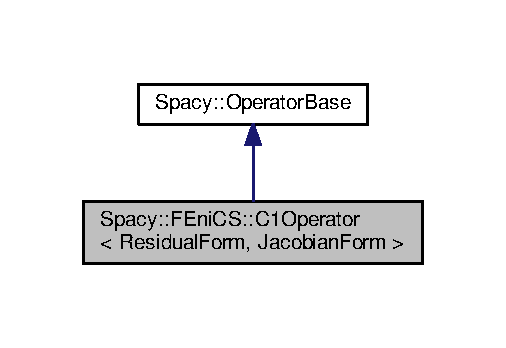
\includegraphics[width=243pt]{classSpacy_1_1FEniCS_1_1C1Operator__inherit__graph}
\end{center}
\end{figure}


Collaboration diagram for Spacy\+:\+:F\+Eni\+C\+S\+:\+:C1\+Operator$<$ Residual\+Form, Jacobian\+Form $>$\+:\nopagebreak
\begin{figure}[H]
\begin{center}
\leavevmode
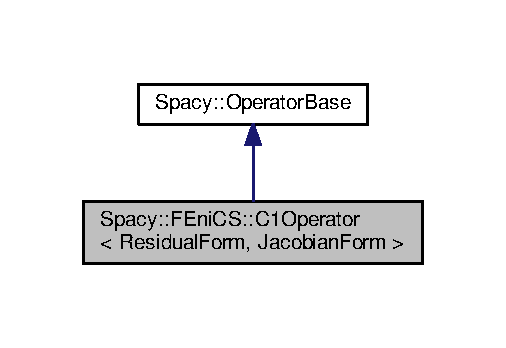
\includegraphics[width=243pt]{classSpacy_1_1FEniCS_1_1C1Operator__coll__graph}
\end{center}
\end{figure}
\subsection*{Public Member Functions}
\begin{DoxyCompactItemize}
\item 
\hyperlink{classSpacy_1_1FEniCS_1_1C1Operator_af23d84bd48d0902011bf80ba2f4cd394}{C1\+Operator} (const Residual\+Form \&F, const Jacobian\+Form \&J, const std\+::vector$<$ const dolfin\+::\+Dirichlet\+B\+C $\ast$ $>$ \&bcs, \hyperlink{classSpacy_1_1VectorSpace}{Vector\+Space} \&\hyperlink{classSpacy_1_1OperatorBase_a2588f9b3e0188820c4c494e63293dc6f}{domain}, \hyperlink{classSpacy_1_1VectorSpace}{Vector\+Space} \&\hyperlink{classSpacy_1_1OperatorBase_ab19d3b7a6f290b1079248f1e567e53d6}{range})
\begin{DoxyCompactList}\small\item\em Construct operator for F\+Enics. \end{DoxyCompactList}\item 
\hyperlink{classSpacy_1_1FEniCS_1_1C1Operator_afe6c4eb8960290212a16a1eca2267b48}{C1\+Operator} (const Residual\+Form \&F, const Jacobian\+Form \&J, \hyperlink{classSpacy_1_1VectorSpace}{Vector\+Space} \&\hyperlink{classSpacy_1_1OperatorBase_a2588f9b3e0188820c4c494e63293dc6f}{domain}, \hyperlink{classSpacy_1_1VectorSpace}{Vector\+Space} \&\hyperlink{classSpacy_1_1OperatorBase_ab19d3b7a6f290b1079248f1e567e53d6}{range})
\begin{DoxyCompactList}\small\item\em Construct operator without boundary conditions for F\+Enics. \end{DoxyCompactList}\item 
\hypertarget{classSpacy_1_1FEniCS_1_1C1Operator_a4ab2b79f50f05b4cc4403269dad87e1e}{}{\bfseries C1\+Operator} (\hyperlink{classSpacy_1_1FEniCS_1_1C1Operator}{C1\+Operator} \&\&other)\label{classSpacy_1_1FEniCS_1_1C1Operator_a4ab2b79f50f05b4cc4403269dad87e1e}

\item 
\hypertarget{classSpacy_1_1FEniCS_1_1C1Operator_a8bedc9295f43ebe21be9e2a9337da1e5}{}{\bfseries C1\+Operator} (const \hyperlink{classSpacy_1_1FEniCS_1_1C1Operator}{C1\+Operator} \&other)\label{classSpacy_1_1FEniCS_1_1C1Operator_a8bedc9295f43ebe21be9e2a9337da1e5}

\item 
\hypertarget{classSpacy_1_1FEniCS_1_1C1Operator_a1e74d332b9cb30ed83d757a39453c47c}{}\hyperlink{classSpacy_1_1FEniCS_1_1C1Operator}{C1\+Operator} \& {\bfseries operator=} (const \hyperlink{classSpacy_1_1FEniCS_1_1C1Operator}{C1\+Operator} \&other)\label{classSpacy_1_1FEniCS_1_1C1Operator_a1e74d332b9cb30ed83d757a39453c47c}

\item 
\hypertarget{classSpacy_1_1FEniCS_1_1C1Operator_ae611721c1f172413877c91a3e99ae69b}{}\hyperlink{classSpacy_1_1FEniCS_1_1C1Operator}{C1\+Operator} \& {\bfseries operator=} (\hyperlink{classSpacy_1_1FEniCS_1_1C1Operator}{C1\+Operator} \&\&other)\label{classSpacy_1_1FEniCS_1_1C1Operator_ae611721c1f172413877c91a3e99ae69b}

\item 
\hypertarget{classSpacy_1_1FEniCS_1_1C1Operator_a5e2b3831a7583793f6c134eedd2be9bc}{}\+::\hyperlink{classSpacy_1_1Vector}{Spacy\+::\+Vector} \hyperlink{classSpacy_1_1FEniCS_1_1C1Operator_a5e2b3831a7583793f6c134eedd2be9bc}{operator()} (const \+::\hyperlink{classSpacy_1_1Vector}{Spacy\+::\+Vector} \&x) const \label{classSpacy_1_1FEniCS_1_1C1Operator_a5e2b3831a7583793f6c134eedd2be9bc}

\begin{DoxyCompactList}\small\item\em Compute $A(x)$. \end{DoxyCompactList}\item 
\hypertarget{classSpacy_1_1FEniCS_1_1C1Operator_a610d7a4a5daec3b512ab3ccf46a7b9e9}{}\+::\hyperlink{classSpacy_1_1Vector}{Spacy\+::\+Vector} \hyperlink{classSpacy_1_1FEniCS_1_1C1Operator_a610d7a4a5daec3b512ab3ccf46a7b9e9}{d1} (const \+::\hyperlink{classSpacy_1_1Vector}{Spacy\+::\+Vector} \&x, const \+::\hyperlink{classSpacy_1_1Vector}{Spacy\+::\+Vector} \&dx) const \label{classSpacy_1_1FEniCS_1_1C1Operator_a610d7a4a5daec3b512ab3ccf46a7b9e9}

\begin{DoxyCompactList}\small\item\em Compute $A'(x)dx$. \end{DoxyCompactList}\item 
auto \hyperlink{classSpacy_1_1FEniCS_1_1C1Operator_aab603c2b35f2b710b2e646cf3fb7ee9c}{linearization} (const \+::\hyperlink{classSpacy_1_1Vector}{Spacy\+::\+Vector} \&x) const 
\begin{DoxyCompactList}\small\item\em Access $A'(x)$ as linear operator $X\rightarrow Y$. \end{DoxyCompactList}\item 
\hypertarget{classSpacy_1_1OperatorBase_a2588f9b3e0188820c4c494e63293dc6f}{}const \hyperlink{classSpacy_1_1VectorSpace}{Vector\+Space} \& \hyperlink{classSpacy_1_1OperatorBase_a2588f9b3e0188820c4c494e63293dc6f}{domain} () const \label{classSpacy_1_1OperatorBase_a2588f9b3e0188820c4c494e63293dc6f}

\begin{DoxyCompactList}\small\item\em Access domain space $X$. \end{DoxyCompactList}\item 
\hypertarget{classSpacy_1_1OperatorBase_ab19d3b7a6f290b1079248f1e567e53d6}{}const \hyperlink{classSpacy_1_1VectorSpace}{Vector\+Space} \& \hyperlink{classSpacy_1_1OperatorBase_ab19d3b7a6f290b1079248f1e567e53d6}{range} () const \label{classSpacy_1_1OperatorBase_ab19d3b7a6f290b1079248f1e567e53d6}

\begin{DoxyCompactList}\small\item\em Access range space $Y$. \end{DoxyCompactList}\end{DoxyCompactItemize}


\subsection{Detailed Description}
\subsubsection*{template$<$class Residual\+Form, class Jacobian\+Form$>$class Spacy\+::\+F\+Eni\+C\+S\+::\+C1\+Operator$<$ Residual\+Form, Jacobian\+Form $>$}

Operator interface for F\+Eni\+C\+S. Models a differentiable operator $A:X\rightarrow Y$. 

\begin{DoxyWarning}{Warning}
In the .ufl file you have to name the argument of $f$ by \char`\"{}x\char`\"{}! 
\end{DoxyWarning}
\begin{DoxySeeAlso}{See also}
C1\+Operator, \hyperlink{group__ConceptGroup_C1OperatorConceptAnchor}{C1\+Operator\+Concept} 
\end{DoxySeeAlso}


\subsection{Constructor \& Destructor Documentation}
\hypertarget{classSpacy_1_1FEniCS_1_1C1Operator_af23d84bd48d0902011bf80ba2f4cd394}{}\index{Spacy\+::\+F\+Eni\+C\+S\+::\+C1\+Operator@{Spacy\+::\+F\+Eni\+C\+S\+::\+C1\+Operator}!C1\+Operator@{C1\+Operator}}
\index{C1\+Operator@{C1\+Operator}!Spacy\+::\+F\+Eni\+C\+S\+::\+C1\+Operator@{Spacy\+::\+F\+Eni\+C\+S\+::\+C1\+Operator}}
\subsubsection[{C1\+Operator}]{\setlength{\rightskip}{0pt plus 5cm}template$<$class Residual\+Form , class Jacobian\+Form $>$ {\bf Spacy\+::\+F\+Eni\+C\+S\+::\+C1\+Operator}$<$ Residual\+Form, Jacobian\+Form $>$\+::{\bf C1\+Operator} (
\begin{DoxyParamCaption}
\item[{const Residual\+Form \&}]{F, }
\item[{const Jacobian\+Form \&}]{J, }
\item[{const std\+::vector$<$ const dolfin\+::\+Dirichlet\+B\+C $\ast$ $>$ \&}]{bcs, }
\item[{{\bf Vector\+Space} \&}]{domain, }
\item[{{\bf Vector\+Space} \&}]{range}
\end{DoxyParamCaption}
)\hspace{0.3cm}{\ttfamily [inline]}}\label{classSpacy_1_1FEniCS_1_1C1Operator_af23d84bd48d0902011bf80ba2f4cd394}


Construct operator for F\+Enics. 


\begin{DoxyParams}{Parameters}
{\em F} & Residual form for the evaluation of $A$ \\
\hline
{\em J} & Jacobian form for the evaluation of $A'$ \\
\hline
{\em bcs} & Dirichlet boundary conditions \\
\hline
{\em domain} & domain space $X$ \\
\hline
{\em range} & range space $Y$ \\
\hline
\end{DoxyParams}
\hypertarget{classSpacy_1_1FEniCS_1_1C1Operator_afe6c4eb8960290212a16a1eca2267b48}{}\index{Spacy\+::\+F\+Eni\+C\+S\+::\+C1\+Operator@{Spacy\+::\+F\+Eni\+C\+S\+::\+C1\+Operator}!C1\+Operator@{C1\+Operator}}
\index{C1\+Operator@{C1\+Operator}!Spacy\+::\+F\+Eni\+C\+S\+::\+C1\+Operator@{Spacy\+::\+F\+Eni\+C\+S\+::\+C1\+Operator}}
\subsubsection[{C1\+Operator}]{\setlength{\rightskip}{0pt plus 5cm}template$<$class Residual\+Form , class Jacobian\+Form $>$ {\bf Spacy\+::\+F\+Eni\+C\+S\+::\+C1\+Operator}$<$ Residual\+Form, Jacobian\+Form $>$\+::{\bf C1\+Operator} (
\begin{DoxyParamCaption}
\item[{const Residual\+Form \&}]{F, }
\item[{const Jacobian\+Form \&}]{J, }
\item[{{\bf Vector\+Space} \&}]{domain, }
\item[{{\bf Vector\+Space} \&}]{range}
\end{DoxyParamCaption}
)\hspace{0.3cm}{\ttfamily [inline]}}\label{classSpacy_1_1FEniCS_1_1C1Operator_afe6c4eb8960290212a16a1eca2267b48}


Construct operator without boundary conditions for F\+Enics. 


\begin{DoxyParams}{Parameters}
{\em F} & Residual form for the evaluation of $A$ \\
\hline
{\em J} & Jacobian form for the evaluation of $A'$ \\
\hline
{\em domain} & domain space $X$ \\
\hline
{\em range} & range space $Y$ \\
\hline
\end{DoxyParams}


\subsection{Member Function Documentation}
\hypertarget{classSpacy_1_1FEniCS_1_1C1Operator_aab603c2b35f2b710b2e646cf3fb7ee9c}{}\index{Spacy\+::\+F\+Eni\+C\+S\+::\+C1\+Operator@{Spacy\+::\+F\+Eni\+C\+S\+::\+C1\+Operator}!linearization@{linearization}}
\index{linearization@{linearization}!Spacy\+::\+F\+Eni\+C\+S\+::\+C1\+Operator@{Spacy\+::\+F\+Eni\+C\+S\+::\+C1\+Operator}}
\subsubsection[{linearization}]{\setlength{\rightskip}{0pt plus 5cm}template$<$class Residual\+Form , class Jacobian\+Form $>$ auto {\bf Spacy\+::\+F\+Eni\+C\+S\+::\+C1\+Operator}$<$ Residual\+Form, Jacobian\+Form $>$\+::linearization (
\begin{DoxyParamCaption}
\item[{const \+::{\bf Spacy\+::\+Vector} \&}]{x}
\end{DoxyParamCaption}
) const\hspace{0.3cm}{\ttfamily [inline]}}\label{classSpacy_1_1FEniCS_1_1C1Operator_aab603c2b35f2b710b2e646cf3fb7ee9c}


Access $A'(x)$ as linear operator $X\rightarrow Y$. 

\begin{DoxySeeAlso}{See also}
\hyperlink{classSpacy_1_1FEniCS_1_1LinearOperator}{Linear\+Operator}, \hyperlink{classSpacy_1_1LinearOperator}{Spacy\+::\+Linear\+Operator} 
\end{DoxySeeAlso}


The documentation for this class was generated from the following file\+:\begin{DoxyCompactItemize}
\item 
Spacy/\+Adapter/\+F\+Eni\+C\+S/c1\+Operator.\+hh\end{DoxyCompactItemize}

\hypertarget{classSpacy_1_1Kaskade_1_1C1Operator}{}\section{Spacy\+:\+:Kaskade\+:\+:C1\+Operator$<$ Operator\+Definition $>$ Class Template Reference}
\label{classSpacy_1_1Kaskade_1_1C1Operator}\index{Spacy\+::\+Kaskade\+::\+C1\+Operator$<$ Operator\+Definition $>$@{Spacy\+::\+Kaskade\+::\+C1\+Operator$<$ Operator\+Definition $>$}}


Operator interface for Kaskade 7. Models a differentiable operator $A:X\rightarrow Y$.  




{\ttfamily \#include $<$c1\+Operator.\+hh$>$}



Inheritance diagram for Spacy\+:\+:Kaskade\+:\+:C1\+Operator$<$ Operator\+Definition $>$\+:\nopagebreak
\begin{figure}[H]
\begin{center}
\leavevmode
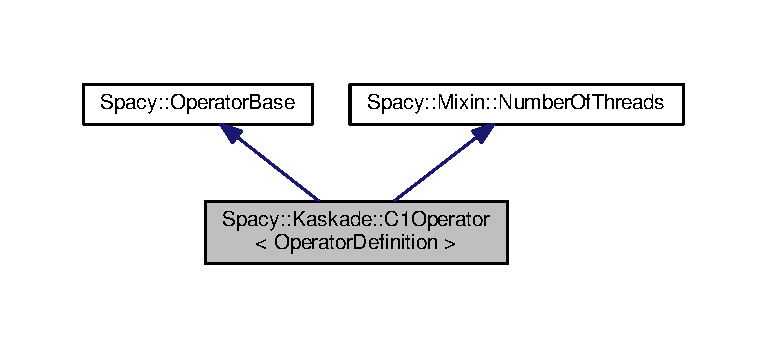
\includegraphics[width=350pt]{classSpacy_1_1Kaskade_1_1C1Operator__inherit__graph}
\end{center}
\end{figure}


Collaboration diagram for Spacy\+:\+:Kaskade\+:\+:C1\+Operator$<$ Operator\+Definition $>$\+:\nopagebreak
\begin{figure}[H]
\begin{center}
\leavevmode
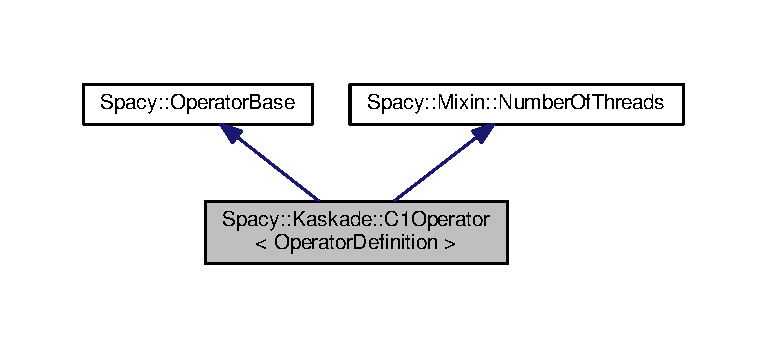
\includegraphics[width=350pt]{classSpacy_1_1Kaskade_1_1C1Operator__coll__graph}
\end{center}
\end{figure}
\subsection*{Public Member Functions}
\begin{DoxyCompactItemize}
\item 
\hyperlink{classSpacy_1_1Kaskade_1_1C1Operator_aa31e9f54fcbb4eb6c40c1cd467d25836}{C1\+Operator} (const Operator\+Definition \&f, const \hyperlink{classSpacy_1_1VectorSpace}{Vector\+Space} \&\hyperlink{classSpacy_1_1OperatorBase_a2588f9b3e0188820c4c494e63293dc6f}{domain}, const \hyperlink{classSpacy_1_1VectorSpace}{Vector\+Space} \&\hyperlink{classSpacy_1_1OperatorBase_ab19d3b7a6f290b1079248f1e567e53d6}{range}, int rbegin=0, int rend=Operator\+Definition\+::\+Ansatz\+Vars\+::no\+Of\+Variables, int cbegin=0, int cend=Operator\+Definition\+::\+Test\+Vars\+::no\+Of\+Variables)
\begin{DoxyCompactList}\small\item\em Construct operator for Kaskade 7. \end{DoxyCompactList}\item 
\hyperlink{classSpacy_1_1Kaskade_1_1C1Operator_a69a67a899fb71e106b1371117d006659}{C1\+Operator} (const \hyperlink{classSpacy_1_1Kaskade_1_1C1Operator}{C1\+Operator} \&B)
\begin{DoxyCompactList}\small\item\em Copy constructor. \end{DoxyCompactList}\item 
\hyperlink{classSpacy_1_1Kaskade_1_1C1Operator}{C1\+Operator} \& \hyperlink{classSpacy_1_1Kaskade_1_1C1Operator_ac378b7b319e5160a7ac19a3697b4291a}{operator=} (const \hyperlink{classSpacy_1_1Kaskade_1_1C1Operator}{C1\+Operator} \&B)
\begin{DoxyCompactList}\small\item\em Copy assignment. \end{DoxyCompactList}\item 
\hyperlink{classSpacy_1_1Kaskade_1_1C1Operator_aed7bcf133fe772d9ae4b6ad5dcd5674c}{C1\+Operator} (\hyperlink{classSpacy_1_1Kaskade_1_1C1Operator}{C1\+Operator} \&\&B)=default
\begin{DoxyCompactList}\small\item\em Move constructor. \end{DoxyCompactList}\item 
\hyperlink{classSpacy_1_1Kaskade_1_1C1Operator}{C1\+Operator} \& \hyperlink{classSpacy_1_1Kaskade_1_1C1Operator_ab05b1e6565daf571d60ecf1b4584c991}{operator=} (\hyperlink{classSpacy_1_1Kaskade_1_1C1Operator}{C1\+Operator} \&\&B)=default
\begin{DoxyCompactList}\small\item\em Move assignment. \end{DoxyCompactList}\item 
\+::\hyperlink{classSpacy_1_1Vector}{Spacy\+::\+Vector} \hyperlink{classSpacy_1_1Kaskade_1_1C1Operator_aae23a007cd7a66f90bbb1c93da34735d}{operator()} (const \+::\hyperlink{classSpacy_1_1Vector}{Spacy\+::\+Vector} \&x) const 
\begin{DoxyCompactList}\small\item\em Apply operator. \end{DoxyCompactList}\item 
\+::\hyperlink{classSpacy_1_1Vector}{Spacy\+::\+Vector} \hyperlink{classSpacy_1_1Kaskade_1_1C1Operator_a32cfd05c372cc4bc8d7e0e8aedc1e8b9}{d1} (const \+::\hyperlink{classSpacy_1_1Vector}{Spacy\+::\+Vector} \&x, const \+::\hyperlink{classSpacy_1_1Vector}{Spacy\+::\+Vector} \&dx) const 
\begin{DoxyCompactList}\small\item\em Compute $A'(x)dx$. \end{DoxyCompactList}\item 
\hypertarget{classSpacy_1_1Kaskade_1_1C1Operator_afb9837bb1c40e00b53e7430c745b1931}{}auto \hyperlink{classSpacy_1_1Kaskade_1_1C1Operator_afb9837bb1c40e00b53e7430c745b1931}{linearization} (const \+::\hyperlink{classSpacy_1_1Vector}{Spacy\+::\+Vector} \&x) const \label{classSpacy_1_1Kaskade_1_1C1Operator_afb9837bb1c40e00b53e7430c745b1931}

\begin{DoxyCompactList}\small\item\em Access $A'(x)$ as linear operator $X\rightarrow Y$. \end{DoxyCompactList}\item 
\hypertarget{classSpacy_1_1Kaskade_1_1C1Operator_ab050915a62f3f8bf25e78af1e1289cb8}{}const Kaskade\+Operator \& \hyperlink{classSpacy_1_1Kaskade_1_1C1Operator_ab050915a62f3f8bf25e78af1e1289cb8}{A} () const noexcept\label{classSpacy_1_1Kaskade_1_1C1Operator_ab050915a62f3f8bf25e78af1e1289cb8}

\begin{DoxyCompactList}\small\item\em Access operator representing $A'(x)$. \end{DoxyCompactList}\item 
bool \hyperlink{classSpacy_1_1Kaskade_1_1C1Operator_adb85b50e1cc87fb342412560353c2f73}{only\+Lower\+Triangle} () const noexcept
\begin{DoxyCompactList}\small\item\em Access only\+Lower\+Triangle flag. \end{DoxyCompactList}\item 
void \hyperlink{classSpacy_1_1Kaskade_1_1C1Operator_aa0c69955542db6b0f61807181874b4d9}{set\+Solver\+Creator} (std\+::function$<$ \hyperlink{namespaceSpacy_a4cd614ddb41dd29e68a723dadd5602f2}{Linear\+Solver}(const \hyperlink{classSpacy_1_1Kaskade_1_1LinearOperator}{Linearization} \&)$>$ f)
\begin{DoxyCompactList}\small\item\em Change solver creator. \end{DoxyCompactList}\item 
\hypertarget{classSpacy_1_1OperatorBase_a2588f9b3e0188820c4c494e63293dc6f}{}const \hyperlink{classSpacy_1_1VectorSpace}{Vector\+Space} \& \hyperlink{classSpacy_1_1OperatorBase_a2588f9b3e0188820c4c494e63293dc6f}{domain} () const \label{classSpacy_1_1OperatorBase_a2588f9b3e0188820c4c494e63293dc6f}

\begin{DoxyCompactList}\small\item\em Access domain space $X$. \end{DoxyCompactList}\item 
\hypertarget{classSpacy_1_1OperatorBase_ab19d3b7a6f290b1079248f1e567e53d6}{}const \hyperlink{classSpacy_1_1VectorSpace}{Vector\+Space} \& \hyperlink{classSpacy_1_1OperatorBase_ab19d3b7a6f290b1079248f1e567e53d6}{range} () const \label{classSpacy_1_1OperatorBase_ab19d3b7a6f290b1079248f1e567e53d6}

\begin{DoxyCompactList}\small\item\em Access range space $Y$. \end{DoxyCompactList}\item 
\hypertarget{classSpacy_1_1Mixin_1_1NumberOfThreads_ab0c2fca77cb0d613e3bb8ce5bda11fdc}{}void {\bfseries set\+Number\+Of\+Threads} (unsigned \hyperlink{classSpacy_1_1Mixin_1_1NumberOfThreads_a385963b95b5e1ddf422393146cc71ee1}{n\+Threads}=1)\label{classSpacy_1_1Mixin_1_1NumberOfThreads_ab0c2fca77cb0d613e3bb8ce5bda11fdc}

\item 
\hypertarget{classSpacy_1_1Mixin_1_1NumberOfThreads_a385963b95b5e1ddf422393146cc71ee1}{}unsigned \hyperlink{classSpacy_1_1Mixin_1_1NumberOfThreads_a385963b95b5e1ddf422393146cc71ee1}{n\+Threads} () const noexcept\label{classSpacy_1_1Mixin_1_1NumberOfThreads_a385963b95b5e1ddf422393146cc71ee1}

\begin{DoxyCompactList}\small\item\em Access number of allowed threads. \end{DoxyCompactList}\end{DoxyCompactItemize}


\subsection{Detailed Description}
\subsubsection*{template$<$class Operator\+Definition$>$class Spacy\+::\+Kaskade\+::\+C1\+Operator$<$ Operator\+Definition $>$}

Operator interface for Kaskade 7. Models a differentiable operator $A:X\rightarrow Y$. 

\begin{DoxySeeAlso}{See also}
\hyperlink{classSpacy_1_1C1Operator}{Spacy\+::\+C1\+Operator} 
\end{DoxySeeAlso}


\subsection{Constructor \& Destructor Documentation}
\hypertarget{classSpacy_1_1Kaskade_1_1C1Operator_aa31e9f54fcbb4eb6c40c1cd467d25836}{}\index{Spacy\+::\+Kaskade\+::\+C1\+Operator@{Spacy\+::\+Kaskade\+::\+C1\+Operator}!C1\+Operator@{C1\+Operator}}
\index{C1\+Operator@{C1\+Operator}!Spacy\+::\+Kaskade\+::\+C1\+Operator@{Spacy\+::\+Kaskade\+::\+C1\+Operator}}
\subsubsection[{C1\+Operator}]{\setlength{\rightskip}{0pt plus 5cm}template$<$class Operator\+Definition$>$ {\bf Spacy\+::\+Kaskade\+::\+C1\+Operator}$<$ Operator\+Definition $>$\+::{\bf C1\+Operator} (
\begin{DoxyParamCaption}
\item[{const Operator\+Definition \&}]{f, }
\item[{const {\bf Vector\+Space} \&}]{domain, }
\item[{const {\bf Vector\+Space} \&}]{range, }
\item[{int}]{rbegin = {\ttfamily 0}, }
\item[{int}]{rend = {\ttfamily OperatorDefinition\+:\+:AnsatzVars\+:\+:noOfVariables}, }
\item[{int}]{cbegin = {\ttfamily 0}, }
\item[{int}]{cend = {\ttfamily OperatorDefinition\+:\+:TestVars\+:\+:noOfVariables}}
\end{DoxyParamCaption}
)\hspace{0.3cm}{\ttfamily [inline]}}\label{classSpacy_1_1Kaskade_1_1C1Operator_aa31e9f54fcbb4eb6c40c1cd467d25836}


Construct operator for Kaskade 7. 


\begin{DoxyParams}{Parameters}
{\em f} & operator definition from Kaskade 7 \\
\hline
{\em domain} & domain space \\
\hline
{\em range} & range space \\
\hline
{\em rbegin} & first row to be considered in the definition of f \\
\hline
{\em rend} & one after the last row to be considered in the definition of f \\
\hline
{\em cbegin} & first column to be considered in the definition of f \\
\hline
{\em cend} & one after the last column to be considered in the definition of f\\
\hline
\end{DoxyParams}
The optional parameters rbegin, rend, cbegin and cend can be used to define operators that correspond to parts of a system of equation. \hypertarget{classSpacy_1_1Kaskade_1_1C1Operator_a69a67a899fb71e106b1371117d006659}{}\index{Spacy\+::\+Kaskade\+::\+C1\+Operator@{Spacy\+::\+Kaskade\+::\+C1\+Operator}!C1\+Operator@{C1\+Operator}}
\index{C1\+Operator@{C1\+Operator}!Spacy\+::\+Kaskade\+::\+C1\+Operator@{Spacy\+::\+Kaskade\+::\+C1\+Operator}}
\subsubsection[{C1\+Operator}]{\setlength{\rightskip}{0pt plus 5cm}template$<$class Operator\+Definition$>$ {\bf Spacy\+::\+Kaskade\+::\+C1\+Operator}$<$ Operator\+Definition $>$\+::{\bf C1\+Operator} (
\begin{DoxyParamCaption}
\item[{const {\bf C1\+Operator}$<$ Operator\+Definition $>$ \&}]{B}
\end{DoxyParamCaption}
)\hspace{0.3cm}{\ttfamily [inline]}}\label{classSpacy_1_1Kaskade_1_1C1Operator_a69a67a899fb71e106b1371117d006659}


Copy constructor. 


\begin{DoxyParams}{Parameters}
{\em B} & object to copy from \\
\hline
\end{DoxyParams}
\hypertarget{classSpacy_1_1Kaskade_1_1C1Operator_aed7bcf133fe772d9ae4b6ad5dcd5674c}{}\index{Spacy\+::\+Kaskade\+::\+C1\+Operator@{Spacy\+::\+Kaskade\+::\+C1\+Operator}!C1\+Operator@{C1\+Operator}}
\index{C1\+Operator@{C1\+Operator}!Spacy\+::\+Kaskade\+::\+C1\+Operator@{Spacy\+::\+Kaskade\+::\+C1\+Operator}}
\subsubsection[{C1\+Operator}]{\setlength{\rightskip}{0pt plus 5cm}template$<$class Operator\+Definition$>$ {\bf Spacy\+::\+Kaskade\+::\+C1\+Operator}$<$ Operator\+Definition $>$\+::{\bf C1\+Operator} (
\begin{DoxyParamCaption}
\item[{{\bf C1\+Operator}$<$ Operator\+Definition $>$ \&\&}]{B}
\end{DoxyParamCaption}
)\hspace{0.3cm}{\ttfamily [default]}}\label{classSpacy_1_1Kaskade_1_1C1Operator_aed7bcf133fe772d9ae4b6ad5dcd5674c}


Move constructor. 


\begin{DoxyParams}{Parameters}
{\em B} & object to move from \\
\hline
\end{DoxyParams}


\subsection{Member Function Documentation}
\hypertarget{classSpacy_1_1Kaskade_1_1C1Operator_ac378b7b319e5160a7ac19a3697b4291a}{}\index{Spacy\+::\+Kaskade\+::\+C1\+Operator@{Spacy\+::\+Kaskade\+::\+C1\+Operator}!operator=@{operator=}}
\index{operator=@{operator=}!Spacy\+::\+Kaskade\+::\+C1\+Operator@{Spacy\+::\+Kaskade\+::\+C1\+Operator}}
\subsubsection[{operator=}]{\setlength{\rightskip}{0pt plus 5cm}template$<$class Operator\+Definition$>$ {\bf C1\+Operator}\& {\bf Spacy\+::\+Kaskade\+::\+C1\+Operator}$<$ Operator\+Definition $>$\+::operator= (
\begin{DoxyParamCaption}
\item[{const {\bf C1\+Operator}$<$ Operator\+Definition $>$ \&}]{B}
\end{DoxyParamCaption}
)\hspace{0.3cm}{\ttfamily [inline]}}\label{classSpacy_1_1Kaskade_1_1C1Operator_ac378b7b319e5160a7ac19a3697b4291a}


Copy assignment. 


\begin{DoxyParams}{Parameters}
{\em B} & object to copy from \\
\hline
\end{DoxyParams}
\hypertarget{classSpacy_1_1Kaskade_1_1C1Operator_ab05b1e6565daf571d60ecf1b4584c991}{}\index{Spacy\+::\+Kaskade\+::\+C1\+Operator@{Spacy\+::\+Kaskade\+::\+C1\+Operator}!operator=@{operator=}}
\index{operator=@{operator=}!Spacy\+::\+Kaskade\+::\+C1\+Operator@{Spacy\+::\+Kaskade\+::\+C1\+Operator}}
\subsubsection[{operator=}]{\setlength{\rightskip}{0pt plus 5cm}template$<$class Operator\+Definition$>$ {\bf C1\+Operator}\& {\bf Spacy\+::\+Kaskade\+::\+C1\+Operator}$<$ Operator\+Definition $>$\+::operator= (
\begin{DoxyParamCaption}
\item[{{\bf C1\+Operator}$<$ Operator\+Definition $>$ \&\&}]{B}
\end{DoxyParamCaption}
)\hspace{0.3cm}{\ttfamily [default]}}\label{classSpacy_1_1Kaskade_1_1C1Operator_ab05b1e6565daf571d60ecf1b4584c991}


Move assignment. 


\begin{DoxyParams}{Parameters}
{\em B} & object to move from \\
\hline
\end{DoxyParams}
\hypertarget{classSpacy_1_1Kaskade_1_1C1Operator_aae23a007cd7a66f90bbb1c93da34735d}{}\index{Spacy\+::\+Kaskade\+::\+C1\+Operator@{Spacy\+::\+Kaskade\+::\+C1\+Operator}!operator()@{operator()}}
\index{operator()@{operator()}!Spacy\+::\+Kaskade\+::\+C1\+Operator@{Spacy\+::\+Kaskade\+::\+C1\+Operator}}
\subsubsection[{operator()}]{\setlength{\rightskip}{0pt plus 5cm}template$<$class Operator\+Definition$>$ \+::{\bf Spacy\+::\+Vector} {\bf Spacy\+::\+Kaskade\+::\+C1\+Operator}$<$ Operator\+Definition $>$\+::operator() (
\begin{DoxyParamCaption}
\item[{const \+::{\bf Spacy\+::\+Vector} \&}]{x}
\end{DoxyParamCaption}
) const\hspace{0.3cm}{\ttfamily [inline]}}\label{classSpacy_1_1Kaskade_1_1C1Operator_aae23a007cd7a66f90bbb1c93da34735d}


Apply operator. 


\begin{DoxyParams}{Parameters}
{\em x} & argument \\
\hline
\end{DoxyParams}
\begin{DoxyReturn}{Returns}
$A(x)$ 
\end{DoxyReturn}
\hypertarget{classSpacy_1_1Kaskade_1_1C1Operator_a32cfd05c372cc4bc8d7e0e8aedc1e8b9}{}\index{Spacy\+::\+Kaskade\+::\+C1\+Operator@{Spacy\+::\+Kaskade\+::\+C1\+Operator}!d1@{d1}}
\index{d1@{d1}!Spacy\+::\+Kaskade\+::\+C1\+Operator@{Spacy\+::\+Kaskade\+::\+C1\+Operator}}
\subsubsection[{d1}]{\setlength{\rightskip}{0pt plus 5cm}template$<$class Operator\+Definition$>$ \+::{\bf Spacy\+::\+Vector} {\bf Spacy\+::\+Kaskade\+::\+C1\+Operator}$<$ Operator\+Definition $>$\+::d1 (
\begin{DoxyParamCaption}
\item[{const \+::{\bf Spacy\+::\+Vector} \&}]{x, }
\item[{const \+::{\bf Spacy\+::\+Vector} \&}]{dx}
\end{DoxyParamCaption}
) const\hspace{0.3cm}{\ttfamily [inline]}}\label{classSpacy_1_1Kaskade_1_1C1Operator_a32cfd05c372cc4bc8d7e0e8aedc1e8b9}


Compute $A'(x)dx$. 


\begin{DoxyParams}{Parameters}
{\em x} & current iterate \\
\hline
{\em dx} & correction \\
\hline
\end{DoxyParams}
\begin{DoxyReturn}{Returns}
$A'(x)dx$ 
\end{DoxyReturn}
\hypertarget{classSpacy_1_1Kaskade_1_1C1Operator_adb85b50e1cc87fb342412560353c2f73}{}\index{Spacy\+::\+Kaskade\+::\+C1\+Operator@{Spacy\+::\+Kaskade\+::\+C1\+Operator}!only\+Lower\+Triangle@{only\+Lower\+Triangle}}
\index{only\+Lower\+Triangle@{only\+Lower\+Triangle}!Spacy\+::\+Kaskade\+::\+C1\+Operator@{Spacy\+::\+Kaskade\+::\+C1\+Operator}}
\subsubsection[{only\+Lower\+Triangle}]{\setlength{\rightskip}{0pt plus 5cm}template$<$class Operator\+Definition$>$ bool {\bf Spacy\+::\+Kaskade\+::\+C1\+Operator}$<$ Operator\+Definition $>$\+::only\+Lower\+Triangle (
\begin{DoxyParamCaption}
{}
\end{DoxyParamCaption}
) const\hspace{0.3cm}{\ttfamily [inline]}, {\ttfamily [noexcept]}}\label{classSpacy_1_1Kaskade_1_1C1Operator_adb85b50e1cc87fb342412560353c2f73}


Access only\+Lower\+Triangle flag. 

\begin{DoxyReturn}{Returns}
true if only the lower triangle of a symmetric matrix is stored in the operator definition, else false 
\end{DoxyReturn}
\hypertarget{classSpacy_1_1Kaskade_1_1C1Operator_aa0c69955542db6b0f61807181874b4d9}{}\index{Spacy\+::\+Kaskade\+::\+C1\+Operator@{Spacy\+::\+Kaskade\+::\+C1\+Operator}!set\+Solver\+Creator@{set\+Solver\+Creator}}
\index{set\+Solver\+Creator@{set\+Solver\+Creator}!Spacy\+::\+Kaskade\+::\+C1\+Operator@{Spacy\+::\+Kaskade\+::\+C1\+Operator}}
\subsubsection[{set\+Solver\+Creator}]{\setlength{\rightskip}{0pt plus 5cm}template$<$class Operator\+Definition$>$ void {\bf Spacy\+::\+Kaskade\+::\+C1\+Operator}$<$ Operator\+Definition $>$\+::set\+Solver\+Creator (
\begin{DoxyParamCaption}
\item[{std\+::function$<$ {\bf Linear\+Solver}(const {\bf Linearization} \&)$>$}]{f}
\end{DoxyParamCaption}
)\hspace{0.3cm}{\ttfamily [inline]}}\label{classSpacy_1_1Kaskade_1_1C1Operator_aa0c69955542db6b0f61807181874b4d9}


Change solver creator. 


\begin{DoxyParams}{Parameters}
{\em f} & function/functor for the creation of a linear solver \\
\hline
\end{DoxyParams}


The documentation for this class was generated from the following file\+:\begin{DoxyCompactItemize}
\item 
Spacy/\+Adapter/\+Kaskade/c1\+Operator.\+hh\end{DoxyCompactItemize}

\hypertarget{classSpacy_1_1FEniCS_1_1C2Functional}{}\section{Spacy\+:\+:F\+Eni\+C\+S\+:\+:C2\+Functional$<$ F, D\+F, D\+D\+F $>$ Class Template Reference}
\label{classSpacy_1_1FEniCS_1_1C2Functional}\index{Spacy\+::\+F\+Eni\+C\+S\+::\+C2\+Functional$<$ F, D\+F, D\+D\+F $>$@{Spacy\+::\+F\+Eni\+C\+S\+::\+C2\+Functional$<$ F, D\+F, D\+D\+F $>$}}


Functional interface for F\+Eni\+C\+S. Models a twice differentiable functional $f:X\rightarrow \mathbb{R}$.  




{\ttfamily \#include $<$c2\+Functional.\+hh$>$}



Inheritance diagram for Spacy\+:\+:F\+Eni\+C\+S\+:\+:C2\+Functional$<$ F, D\+F, D\+D\+F $>$\+:\nopagebreak
\begin{figure}[H]
\begin{center}
\leavevmode
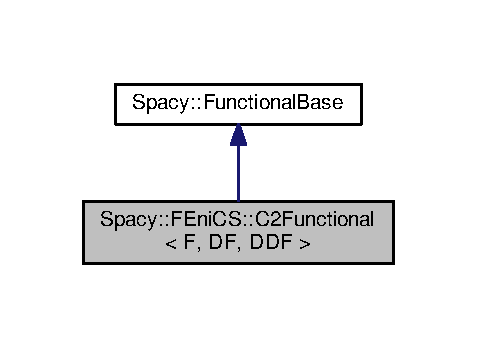
\includegraphics[width=229pt]{classSpacy_1_1FEniCS_1_1C2Functional__inherit__graph}
\end{center}
\end{figure}


Collaboration diagram for Spacy\+:\+:F\+Eni\+C\+S\+:\+:C2\+Functional$<$ F, D\+F, D\+D\+F $>$\+:\nopagebreak
\begin{figure}[H]
\begin{center}
\leavevmode
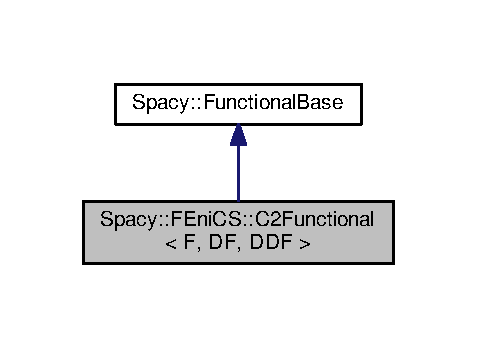
\includegraphics[width=229pt]{classSpacy_1_1FEniCS_1_1C2Functional__coll__graph}
\end{center}
\end{figure}
\subsection*{Public Member Functions}
\begin{DoxyCompactItemize}
\item 
\hyperlink{classSpacy_1_1FEniCS_1_1C2Functional_a8f32c233a72dc3d25a656c1db12af943}{C2\+Functional} (const F \&f, const D\+F \&J, const D\+D\+F \&H, const std\+::vector$<$ const dolfin\+::\+Dirichlet\+B\+C $\ast$ $>$ \&bcs, const \hyperlink{classSpacy_1_1VectorSpace}{Vector\+Space} \&\hyperlink{classSpacy_1_1FunctionalBase_a2d3397deb9fa1ad85ed04e37a03b3aa6}{domain})
\begin{DoxyCompactList}\small\item\em Construct functional for F\+Enics. \end{DoxyCompactList}\item 
\hyperlink{classSpacy_1_1FEniCS_1_1C2Functional_addb84a06f7f82969c57e5bf1b65f2b68}{C2\+Functional} (const \hyperlink{classSpacy_1_1FEniCS_1_1C2Functional}{C2\+Functional} \&g)
\begin{DoxyCompactList}\small\item\em Copy constructor. \end{DoxyCompactList}\item 
\hyperlink{classSpacy_1_1FEniCS_1_1C2Functional}{C2\+Functional} \& \hyperlink{classSpacy_1_1FEniCS_1_1C2Functional_ab9ff23de1e812f6782b7db6ec01e0f4c}{operator=} (const \hyperlink{classSpacy_1_1FEniCS_1_1C2Functional}{C2\+Functional} \&g)
\begin{DoxyCompactList}\small\item\em Copy assignment. \end{DoxyCompactList}\item 
\hyperlink{classSpacy_1_1FEniCS_1_1C2Functional_af9ac63335fc062d18e08fa186312b5a2}{C2\+Functional} (\hyperlink{classSpacy_1_1FEniCS_1_1C2Functional}{C2\+Functional} \&\&g)
\begin{DoxyCompactList}\small\item\em Move constructor. \end{DoxyCompactList}\item 
\hyperlink{classSpacy_1_1FEniCS_1_1C2Functional}{C2\+Functional} \& \hyperlink{classSpacy_1_1FEniCS_1_1C2Functional_a96a909732f7f098d67ee5eba20406337}{operator=} (\hyperlink{classSpacy_1_1FEniCS_1_1C2Functional}{C2\+Functional} \&\&g)
\begin{DoxyCompactList}\small\item\em Move assignment. \end{DoxyCompactList}\item 
\hyperlink{classSpacy_1_1Real}{Real} \hyperlink{classSpacy_1_1FEniCS_1_1C2Functional_abbf25dfc8e8c40edd3ac2dfb61030599}{operator()} (const \+::\hyperlink{classSpacy_1_1Vector}{Spacy\+::\+Vector} \&x) const 
\begin{DoxyCompactList}\small\item\em Apply functional. \end{DoxyCompactList}\item 
\+::\hyperlink{classSpacy_1_1Vector}{Spacy\+::\+Vector} \hyperlink{classSpacy_1_1FEniCS_1_1C2Functional_ab9b10dc982f81093c3125027b46c5876}{d1} (const \+::\hyperlink{classSpacy_1_1Vector}{Spacy\+::\+Vector} \&x) const 
\begin{DoxyCompactList}\small\item\em Compute first directional derivative $f'(x) \in X^* $. \end{DoxyCompactList}\item 
\+::\hyperlink{classSpacy_1_1Vector}{Spacy\+::\+Vector} \hyperlink{classSpacy_1_1FEniCS_1_1C2Functional_affc6728db99f20f57ce75f16799084b4}{d2} (const \+::\hyperlink{classSpacy_1_1Vector}{Spacy\+::\+Vector} \&x, const \+::\hyperlink{classSpacy_1_1Vector}{Spacy\+::\+Vector} \&dx) const 
\begin{DoxyCompactList}\small\item\em Compute second directional derivative $f''(x)dx\in X^* $. \end{DoxyCompactList}\item 
auto \hyperlink{classSpacy_1_1FEniCS_1_1C2Functional_aceec6783f701e121b35ffa482629e1dd}{hessian} (const \+::\hyperlink{classSpacy_1_1Vector}{Spacy\+::\+Vector} \&x) const 
\begin{DoxyCompactList}\small\item\em Access $f''(x)$ as linear operator $X\rightarrow X^*$. \end{DoxyCompactList}\item 
\hypertarget{classSpacy_1_1FunctionalBase_a2d3397deb9fa1ad85ed04e37a03b3aa6}{}const \hyperlink{classSpacy_1_1VectorSpace}{Vector\+Space} \& \hyperlink{classSpacy_1_1FunctionalBase_a2d3397deb9fa1ad85ed04e37a03b3aa6}{domain} () const \label{classSpacy_1_1FunctionalBase_a2d3397deb9fa1ad85ed04e37a03b3aa6}

\begin{DoxyCompactList}\small\item\em Access domain space $X$. \end{DoxyCompactList}\end{DoxyCompactItemize}


\subsection{Detailed Description}
\subsubsection*{template$<$class F, class D\+F, class D\+D\+F$>$class Spacy\+::\+F\+Eni\+C\+S\+::\+C2\+Functional$<$ F, D\+F, D\+D\+F $>$}

Functional interface for F\+Eni\+C\+S. Models a twice differentiable functional $f:X\rightarrow \mathbb{R}$. 


\begin{DoxyTemplParams}{Template Parameters}
{\em F} & dolfin\+::\+Form describing the functional value \\
\hline
{\em D\+F} & dolfin\+::\+Form describing the derivative \\
\hline
{\em D\+D\+F} & dolfin\+::\+Form describing the second derivative \\
\hline
\end{DoxyTemplParams}
\begin{DoxyWarning}{Warning}
In the .ufl file you have to name the argument of $f$ by \char`\"{}x\char`\"{}! 
\end{DoxyWarning}
\begin{DoxySeeAlso}{See also}
\hyperlink{classSpacy_1_1C2Functional}{Spacy\+::\+C2\+Functional} 
\end{DoxySeeAlso}


\subsection{Constructor \& Destructor Documentation}
\hypertarget{classSpacy_1_1FEniCS_1_1C2Functional_a8f32c233a72dc3d25a656c1db12af943}{}\index{Spacy\+::\+F\+Eni\+C\+S\+::\+C2\+Functional@{Spacy\+::\+F\+Eni\+C\+S\+::\+C2\+Functional}!C2\+Functional@{C2\+Functional}}
\index{C2\+Functional@{C2\+Functional}!Spacy\+::\+F\+Eni\+C\+S\+::\+C2\+Functional@{Spacy\+::\+F\+Eni\+C\+S\+::\+C2\+Functional}}
\subsubsection[{C2\+Functional}]{\setlength{\rightskip}{0pt plus 5cm}template$<$class F, class D\+F, class D\+D\+F$>$ {\bf Spacy\+::\+F\+Eni\+C\+S\+::\+C2\+Functional}$<$ F, D\+F, D\+D\+F $>$\+::{\bf C2\+Functional} (
\begin{DoxyParamCaption}
\item[{const F \&}]{f, }
\item[{const D\+F \&}]{J, }
\item[{const D\+D\+F \&}]{H, }
\item[{const std\+::vector$<$ const dolfin\+::\+Dirichlet\+B\+C $\ast$ $>$ \&}]{bcs, }
\item[{const {\bf Vector\+Space} \&}]{domain}
\end{DoxyParamCaption}
)\hspace{0.3cm}{\ttfamily [inline]}}\label{classSpacy_1_1FEniCS_1_1C2Functional_a8f32c233a72dc3d25a656c1db12af943}


Construct functional for F\+Enics. 


\begin{DoxyParams}{Parameters}
{\em f} & form for the evaluation of $f$. \\
\hline
{\em J} & form for the evaluation of $f'$ \\
\hline
{\em H} & form for the evaluation of $f''$ \\
\hline
{\em bcs} & Dirichlet boundary conditions \\
\hline
{\em space} & domain space $X$ \\
\hline
\end{DoxyParams}
\hypertarget{classSpacy_1_1FEniCS_1_1C2Functional_addb84a06f7f82969c57e5bf1b65f2b68}{}\index{Spacy\+::\+F\+Eni\+C\+S\+::\+C2\+Functional@{Spacy\+::\+F\+Eni\+C\+S\+::\+C2\+Functional}!C2\+Functional@{C2\+Functional}}
\index{C2\+Functional@{C2\+Functional}!Spacy\+::\+F\+Eni\+C\+S\+::\+C2\+Functional@{Spacy\+::\+F\+Eni\+C\+S\+::\+C2\+Functional}}
\subsubsection[{C2\+Functional}]{\setlength{\rightskip}{0pt plus 5cm}template$<$class F, class D\+F, class D\+D\+F$>$ {\bf Spacy\+::\+F\+Eni\+C\+S\+::\+C2\+Functional}$<$ F, D\+F, D\+D\+F $>$\+::{\bf C2\+Functional} (
\begin{DoxyParamCaption}
\item[{const {\bf C2\+Functional}$<$ F, D\+F, D\+D\+F $>$ \&}]{g}
\end{DoxyParamCaption}
)\hspace{0.3cm}{\ttfamily [inline]}}\label{classSpacy_1_1FEniCS_1_1C2Functional_addb84a06f7f82969c57e5bf1b65f2b68}


Copy constructor. 


\begin{DoxyParams}{Parameters}
{\em g} & functional to copy from \\
\hline
\end{DoxyParams}
\hypertarget{classSpacy_1_1FEniCS_1_1C2Functional_af9ac63335fc062d18e08fa186312b5a2}{}\index{Spacy\+::\+F\+Eni\+C\+S\+::\+C2\+Functional@{Spacy\+::\+F\+Eni\+C\+S\+::\+C2\+Functional}!C2\+Functional@{C2\+Functional}}
\index{C2\+Functional@{C2\+Functional}!Spacy\+::\+F\+Eni\+C\+S\+::\+C2\+Functional@{Spacy\+::\+F\+Eni\+C\+S\+::\+C2\+Functional}}
\subsubsection[{C2\+Functional}]{\setlength{\rightskip}{0pt plus 5cm}template$<$class F, class D\+F, class D\+D\+F$>$ {\bf Spacy\+::\+F\+Eni\+C\+S\+::\+C2\+Functional}$<$ F, D\+F, D\+D\+F $>$\+::{\bf C2\+Functional} (
\begin{DoxyParamCaption}
\item[{{\bf C2\+Functional}$<$ F, D\+F, D\+D\+F $>$ \&\&}]{g}
\end{DoxyParamCaption}
)\hspace{0.3cm}{\ttfamily [inline]}}\label{classSpacy_1_1FEniCS_1_1C2Functional_af9ac63335fc062d18e08fa186312b5a2}


Move constructor. 


\begin{DoxyParams}{Parameters}
{\em g} & functional to move from \\
\hline
\end{DoxyParams}


\subsection{Member Function Documentation}
\hypertarget{classSpacy_1_1FEniCS_1_1C2Functional_ab9ff23de1e812f6782b7db6ec01e0f4c}{}\index{Spacy\+::\+F\+Eni\+C\+S\+::\+C2\+Functional@{Spacy\+::\+F\+Eni\+C\+S\+::\+C2\+Functional}!operator=@{operator=}}
\index{operator=@{operator=}!Spacy\+::\+F\+Eni\+C\+S\+::\+C2\+Functional@{Spacy\+::\+F\+Eni\+C\+S\+::\+C2\+Functional}}
\subsubsection[{operator=}]{\setlength{\rightskip}{0pt plus 5cm}template$<$class F, class D\+F, class D\+D\+F$>$ {\bf C2\+Functional}\& {\bf Spacy\+::\+F\+Eni\+C\+S\+::\+C2\+Functional}$<$ F, D\+F, D\+D\+F $>$\+::operator= (
\begin{DoxyParamCaption}
\item[{const {\bf C2\+Functional}$<$ F, D\+F, D\+D\+F $>$ \&}]{g}
\end{DoxyParamCaption}
)\hspace{0.3cm}{\ttfamily [inline]}}\label{classSpacy_1_1FEniCS_1_1C2Functional_ab9ff23de1e812f6782b7db6ec01e0f4c}


Copy assignment. 


\begin{DoxyParams}{Parameters}
{\em g} & functional to copy from \\
\hline
\end{DoxyParams}
\hypertarget{classSpacy_1_1FEniCS_1_1C2Functional_a96a909732f7f098d67ee5eba20406337}{}\index{Spacy\+::\+F\+Eni\+C\+S\+::\+C2\+Functional@{Spacy\+::\+F\+Eni\+C\+S\+::\+C2\+Functional}!operator=@{operator=}}
\index{operator=@{operator=}!Spacy\+::\+F\+Eni\+C\+S\+::\+C2\+Functional@{Spacy\+::\+F\+Eni\+C\+S\+::\+C2\+Functional}}
\subsubsection[{operator=}]{\setlength{\rightskip}{0pt plus 5cm}template$<$class F, class D\+F, class D\+D\+F$>$ {\bf C2\+Functional}\& {\bf Spacy\+::\+F\+Eni\+C\+S\+::\+C2\+Functional}$<$ F, D\+F, D\+D\+F $>$\+::operator= (
\begin{DoxyParamCaption}
\item[{{\bf C2\+Functional}$<$ F, D\+F, D\+D\+F $>$ \&\&}]{g}
\end{DoxyParamCaption}
)\hspace{0.3cm}{\ttfamily [inline]}}\label{classSpacy_1_1FEniCS_1_1C2Functional_a96a909732f7f098d67ee5eba20406337}


Move assignment. 


\begin{DoxyParams}{Parameters}
{\em g} & functional to move from \\
\hline
\end{DoxyParams}
\hypertarget{classSpacy_1_1FEniCS_1_1C2Functional_abbf25dfc8e8c40edd3ac2dfb61030599}{}\index{Spacy\+::\+F\+Eni\+C\+S\+::\+C2\+Functional@{Spacy\+::\+F\+Eni\+C\+S\+::\+C2\+Functional}!operator()@{operator()}}
\index{operator()@{operator()}!Spacy\+::\+F\+Eni\+C\+S\+::\+C2\+Functional@{Spacy\+::\+F\+Eni\+C\+S\+::\+C2\+Functional}}
\subsubsection[{operator()}]{\setlength{\rightskip}{0pt plus 5cm}template$<$class F, class D\+F, class D\+D\+F$>$ {\bf Real} {\bf Spacy\+::\+F\+Eni\+C\+S\+::\+C2\+Functional}$<$ F, D\+F, D\+D\+F $>$\+::operator() (
\begin{DoxyParamCaption}
\item[{const \+::{\bf Spacy\+::\+Vector} \&}]{x}
\end{DoxyParamCaption}
) const\hspace{0.3cm}{\ttfamily [inline]}}\label{classSpacy_1_1FEniCS_1_1C2Functional_abbf25dfc8e8c40edd3ac2dfb61030599}


Apply functional. 


\begin{DoxyParams}{Parameters}
{\em x} & argument \\
\hline
\end{DoxyParams}
\begin{DoxyReturn}{Returns}
$f(x)$ 
\end{DoxyReturn}
\hypertarget{classSpacy_1_1FEniCS_1_1C2Functional_ab9b10dc982f81093c3125027b46c5876}{}\index{Spacy\+::\+F\+Eni\+C\+S\+::\+C2\+Functional@{Spacy\+::\+F\+Eni\+C\+S\+::\+C2\+Functional}!d1@{d1}}
\index{d1@{d1}!Spacy\+::\+F\+Eni\+C\+S\+::\+C2\+Functional@{Spacy\+::\+F\+Eni\+C\+S\+::\+C2\+Functional}}
\subsubsection[{d1}]{\setlength{\rightskip}{0pt plus 5cm}template$<$class F, class D\+F, class D\+D\+F$>$ \+::{\bf Spacy\+::\+Vector} {\bf Spacy\+::\+F\+Eni\+C\+S\+::\+C2\+Functional}$<$ F, D\+F, D\+D\+F $>$\+::d1 (
\begin{DoxyParamCaption}
\item[{const \+::{\bf Spacy\+::\+Vector} \&}]{x}
\end{DoxyParamCaption}
) const\hspace{0.3cm}{\ttfamily [inline]}}\label{classSpacy_1_1FEniCS_1_1C2Functional_ab9b10dc982f81093c3125027b46c5876}


Compute first directional derivative $f'(x) \in X^* $. 


\begin{DoxyParams}{Parameters}
{\em x} & current iterate \\
\hline
\end{DoxyParams}
\begin{DoxyReturn}{Returns}
$f'(x)$ 
\end{DoxyReturn}
\hypertarget{classSpacy_1_1FEniCS_1_1C2Functional_affc6728db99f20f57ce75f16799084b4}{}\index{Spacy\+::\+F\+Eni\+C\+S\+::\+C2\+Functional@{Spacy\+::\+F\+Eni\+C\+S\+::\+C2\+Functional}!d2@{d2}}
\index{d2@{d2}!Spacy\+::\+F\+Eni\+C\+S\+::\+C2\+Functional@{Spacy\+::\+F\+Eni\+C\+S\+::\+C2\+Functional}}
\subsubsection[{d2}]{\setlength{\rightskip}{0pt plus 5cm}template$<$class F, class D\+F, class D\+D\+F$>$ \+::{\bf Spacy\+::\+Vector} {\bf Spacy\+::\+F\+Eni\+C\+S\+::\+C2\+Functional}$<$ F, D\+F, D\+D\+F $>$\+::d2 (
\begin{DoxyParamCaption}
\item[{const \+::{\bf Spacy\+::\+Vector} \&}]{x, }
\item[{const \+::{\bf Spacy\+::\+Vector} \&}]{dx}
\end{DoxyParamCaption}
) const\hspace{0.3cm}{\ttfamily [inline]}}\label{classSpacy_1_1FEniCS_1_1C2Functional_affc6728db99f20f57ce75f16799084b4}


Compute second directional derivative $f''(x)dx\in X^* $. 


\begin{DoxyParams}{Parameters}
{\em x} & current iterate \\
\hline
{\em dx} & perturbation \\
\hline
\end{DoxyParams}
\begin{DoxyReturn}{Returns}
$f''(x)dx$ 
\end{DoxyReturn}
\hypertarget{classSpacy_1_1FEniCS_1_1C2Functional_aceec6783f701e121b35ffa482629e1dd}{}\index{Spacy\+::\+F\+Eni\+C\+S\+::\+C2\+Functional@{Spacy\+::\+F\+Eni\+C\+S\+::\+C2\+Functional}!hessian@{hessian}}
\index{hessian@{hessian}!Spacy\+::\+F\+Eni\+C\+S\+::\+C2\+Functional@{Spacy\+::\+F\+Eni\+C\+S\+::\+C2\+Functional}}
\subsubsection[{hessian}]{\setlength{\rightskip}{0pt plus 5cm}template$<$class F, class D\+F, class D\+D\+F$>$ auto {\bf Spacy\+::\+F\+Eni\+C\+S\+::\+C2\+Functional}$<$ F, D\+F, D\+D\+F $>$\+::hessian (
\begin{DoxyParamCaption}
\item[{const \+::{\bf Spacy\+::\+Vector} \&}]{x}
\end{DoxyParamCaption}
) const\hspace{0.3cm}{\ttfamily [inline]}}\label{classSpacy_1_1FEniCS_1_1C2Functional_aceec6783f701e121b35ffa482629e1dd}


Access $f''(x)$ as linear operator $X\rightarrow X^*$. 


\begin{DoxyParams}{Parameters}
{\em x} & point of linearization \\
\hline
\end{DoxyParams}


The documentation for this class was generated from the following file\+:\begin{DoxyCompactItemize}
\item 
Spacy/\+Adapter/\+F\+Eni\+C\+S/c2\+Functional.\+hh\end{DoxyCompactItemize}

\hypertarget{classSpacy_1_1Kaskade_1_1C2Functional}{}\section{Spacy\+:\+:Kaskade\+:\+:C2\+Functional$<$ Functional\+Definition $>$ Class Template Reference}
\label{classSpacy_1_1Kaskade_1_1C2Functional}\index{Spacy\+::\+Kaskade\+::\+C2\+Functional$<$ Functional\+Definition $>$@{Spacy\+::\+Kaskade\+::\+C2\+Functional$<$ Functional\+Definition $>$}}


Functional interface for Kaskade 7. Models a twice differentiable functional $f:X\rightarrow \mathbb{R}$.  




{\ttfamily \#include $<$c2\+Functional.\+hh$>$}



Inheritance diagram for Spacy\+:\+:Kaskade\+:\+:C2\+Functional$<$ Functional\+Definition $>$\+:\nopagebreak
\begin{figure}[H]
\begin{center}
\leavevmode
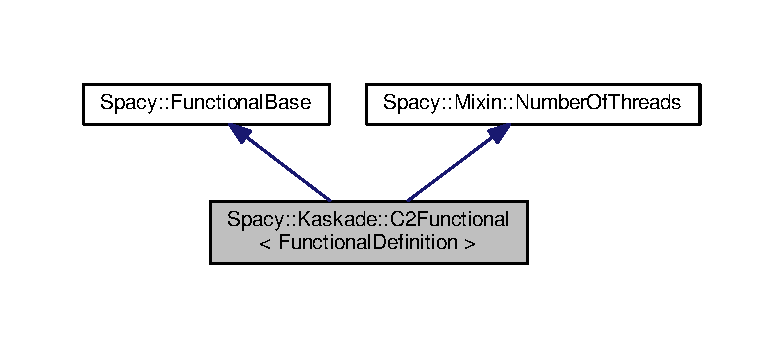
\includegraphics[width=350pt]{classSpacy_1_1Kaskade_1_1C2Functional__inherit__graph}
\end{center}
\end{figure}


Collaboration diagram for Spacy\+:\+:Kaskade\+:\+:C2\+Functional$<$ Functional\+Definition $>$\+:\nopagebreak
\begin{figure}[H]
\begin{center}
\leavevmode
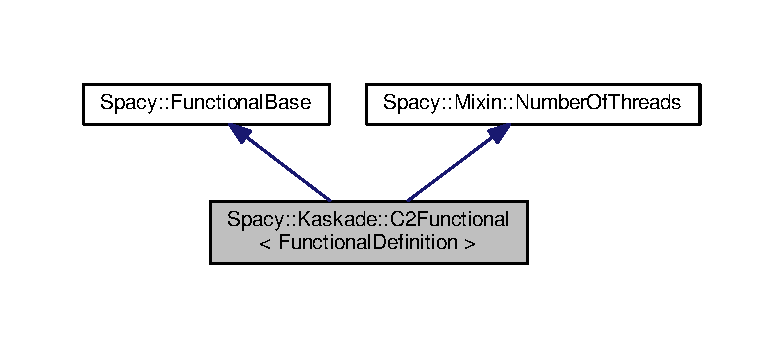
\includegraphics[width=350pt]{classSpacy_1_1Kaskade_1_1C2Functional__coll__graph}
\end{center}
\end{figure}
\subsection*{Public Types}
\begin{DoxyCompactItemize}
\item 
\hypertarget{classSpacy_1_1Kaskade_1_1C2Functional_a7f55d083d721b515160ce43336520e4e}{}using \hyperlink{classSpacy_1_1Kaskade_1_1C2Functional_a7f55d083d721b515160ce43336520e4e}{Variable\+Set\+Description} = typename Functional\+Definition\+::\+Ansatz\+Vars\label{classSpacy_1_1Kaskade_1_1C2Functional_a7f55d083d721b515160ce43336520e4e}

\begin{DoxyCompactList}\small\item\em Kaskade\+::\+Variable\+Set\+Description \end{DoxyCompactList}\item 
\hypertarget{classSpacy_1_1Kaskade_1_1C2Functional_a7845e44764fb2913ebc32153d6d90edf}{}using \hyperlink{classSpacy_1_1Kaskade_1_1C2Functional_a7845e44764fb2913ebc32153d6d90edf}{Coefficient\+Vector} = typename Variable\+Set\+Description\+::template Coefficient\+Vector\+Representation$<$$>$\+::type\label{classSpacy_1_1Kaskade_1_1C2Functional_a7845e44764fb2913ebc32153d6d90edf}

\begin{DoxyCompactList}\small\item\em Coefficient vector type. \end{DoxyCompactList}\item 
\hypertarget{classSpacy_1_1Kaskade_1_1C2Functional_afb866208161b4421f74aab07f50af065}{}using \hyperlink{classSpacy_1_1Kaskade_1_1C2Functional_afb866208161b4421f74aab07f50af065}{Spaces} = typename Variable\+Set\+Description\+::\+Spaces\label{classSpacy_1_1Kaskade_1_1C2Functional_afb866208161b4421f74aab07f50af065}

\begin{DoxyCompactList}\small\item\em boost\+::fusion\+::vector$<$const Space0$\ast$,const Space1$\ast$,...$>$ \end{DoxyCompactList}\item 
\hypertarget{classSpacy_1_1Kaskade_1_1C2Functional_ac4a1a2e519af22616ae7d6214c95b1ed}{}using \hyperlink{classSpacy_1_1Kaskade_1_1C2Functional_ac4a1a2e519af22616ae7d6214c95b1ed}{Assembler} = \+::Kaskade\+::\+Variational\+Functional\+Assembler$<$ \+::Kaskade\+::\+Linearization\+At$<$ Functional\+Definition $>$ $>$\label{classSpacy_1_1Kaskade_1_1C2Functional_ac4a1a2e519af22616ae7d6214c95b1ed}

\begin{DoxyCompactList}\small\item\em Kaskade\+::\+Variational\+Functional\+Assembler \end{DoxyCompactList}\item 
\hypertarget{classSpacy_1_1Kaskade_1_1C2Functional_aa7247706c3561818b2bf7d84c8841fe5}{}using \hyperlink{classSpacy_1_1Kaskade_1_1C2Functional_aa7247706c3561818b2bf7d84c8841fe5}{Matrix} = \+::Kaskade\+::\+Matrix\+As\+Triplet$<$ double $>$\label{classSpacy_1_1Kaskade_1_1C2Functional_aa7247706c3561818b2bf7d84c8841fe5}

\begin{DoxyCompactList}\small\item\em Matrix type. \end{DoxyCompactList}\item 
\hypertarget{classSpacy_1_1Kaskade_1_1C2Functional_af530f936729e854d2fd1401526149ba1}{}using \hyperlink{classSpacy_1_1Kaskade_1_1C2Functional_af530f936729e854d2fd1401526149ba1}{Kaskade\+Operator} = \+::Kaskade\+::\+Matrix\+Represented\+Operator$<$ \hyperlink{classSpacy_1_1Kaskade_1_1C2Functional_aa7247706c3561818b2bf7d84c8841fe5}{Matrix}, \hyperlink{classSpacy_1_1Kaskade_1_1C2Functional_a7845e44764fb2913ebc32153d6d90edf}{Coefficient\+Vector}, \hyperlink{classSpacy_1_1Kaskade_1_1C2Functional_a7845e44764fb2913ebc32153d6d90edf}{Coefficient\+Vector} $>$\label{classSpacy_1_1Kaskade_1_1C2Functional_af530f936729e854d2fd1401526149ba1}

\begin{DoxyCompactList}\small\item\em operator for the description of the second derivative \end{DoxyCompactList}\item 
\hypertarget{classSpacy_1_1Kaskade_1_1C2Functional_a2be6cba631e0718d78b731695f349814}{}using {\bfseries Linearization} = \hyperlink{classSpacy_1_1Kaskade_1_1LinearOperator}{Linear\+Operator}$<$ \hyperlink{classSpacy_1_1Kaskade_1_1C2Functional_a7f55d083d721b515160ce43336520e4e}{Variable\+Set\+Description}, \hyperlink{classSpacy_1_1Kaskade_1_1C2Functional_a7f55d083d721b515160ce43336520e4e}{Variable\+Set\+Description} $>$\label{classSpacy_1_1Kaskade_1_1C2Functional_a2be6cba631e0718d78b731695f349814}

\end{DoxyCompactItemize}
\subsection*{Public Member Functions}
\begin{DoxyCompactItemize}
\item 
\hyperlink{classSpacy_1_1Kaskade_1_1C2Functional_a35511ed1de0b2599efa901f27793dbdc}{C2\+Functional} (const Functional\+Definition \&f, const \hyperlink{classSpacy_1_1VectorSpace}{Vector\+Space} \&\hyperlink{classSpacy_1_1FunctionalBase_a2d3397deb9fa1ad85ed04e37a03b3aa6}{domain}, int rbegin=0, int rend=Functional\+Definition\+::\+Ansatz\+Vars\+::no\+Of\+Variables, int cbegin=0, int cend=Functional\+Definition\+::\+Test\+Vars\+::no\+Of\+Variables)
\begin{DoxyCompactList}\small\item\em Construct a twice differentiable functional $f: X\rightarrow \mathbb{R}$ from Kaskade 7. \end{DoxyCompactList}\item 
\hyperlink{classSpacy_1_1Kaskade_1_1C2Functional_a3d4246d31cffe9ea79cca4ab7c539ede}{C2\+Functional} (const \hyperlink{classSpacy_1_1Kaskade_1_1C2Functional}{C2\+Functional} \&g)
\begin{DoxyCompactList}\small\item\em Copy constructor. \end{DoxyCompactList}\item 
\hyperlink{classSpacy_1_1Kaskade_1_1C2Functional}{C2\+Functional} \& \hyperlink{classSpacy_1_1Kaskade_1_1C2Functional_a1e24c0959890ba4caf0531cf47f3bee5}{operator=} (const \hyperlink{classSpacy_1_1Kaskade_1_1C2Functional}{C2\+Functional} \&g)
\begin{DoxyCompactList}\small\item\em Copy assignment. \end{DoxyCompactList}\item 
\hyperlink{classSpacy_1_1Kaskade_1_1C2Functional_adf3cb62771e39a351db349005ec6bc36}{C2\+Functional} (\hyperlink{classSpacy_1_1Kaskade_1_1C2Functional}{C2\+Functional} \&\&g)=default
\begin{DoxyCompactList}\small\item\em Move constructor. \end{DoxyCompactList}\item 
\hyperlink{classSpacy_1_1Kaskade_1_1C2Functional}{C2\+Functional} \& \hyperlink{classSpacy_1_1Kaskade_1_1C2Functional_a2cabb743e80fa24c22ef0ac358159323}{operator=} (\hyperlink{classSpacy_1_1Kaskade_1_1C2Functional}{C2\+Functional} \&\&g)=default
\begin{DoxyCompactList}\small\item\em Move assignment. \end{DoxyCompactList}\item 
\hyperlink{classSpacy_1_1Real}{Real} \hyperlink{classSpacy_1_1Kaskade_1_1C2Functional_a74b955be1cc2cb7de4e66b434428fd89}{operator()} (const \+::\hyperlink{classSpacy_1_1Vector}{Spacy\+::\+Vector} \&x) const 
\begin{DoxyCompactList}\small\item\em Apply functional. \end{DoxyCompactList}\item 
\+::\hyperlink{classSpacy_1_1Vector}{Spacy\+::\+Vector} \hyperlink{classSpacy_1_1Kaskade_1_1C2Functional_a69d3260b5313bd495e8f5871b15738db}{d1} (const \+::\hyperlink{classSpacy_1_1Vector}{Spacy\+::\+Vector} \&x) const 
\begin{DoxyCompactList}\small\item\em Compute first directional derivative $f'(x) \in X^* $. \end{DoxyCompactList}\item 
\+::\hyperlink{classSpacy_1_1Vector}{Spacy\+::\+Vector} \hyperlink{classSpacy_1_1Kaskade_1_1C2Functional_a7bd6c110c1f954a92f43f6035787a9f0}{d2} (const \+::\hyperlink{classSpacy_1_1Vector}{Spacy\+::\+Vector} \&x, const \+::\hyperlink{classSpacy_1_1Vector}{Spacy\+::\+Vector} \&dx) const 
\begin{DoxyCompactList}\small\item\em Compute second directional derivative $f''(x)dx\in X^* $. \end{DoxyCompactList}\item 
auto \hyperlink{classSpacy_1_1Kaskade_1_1C2Functional_a73e0b9a2499e89bf85eddf1aa74fe9ba}{hessian} (const \+::\hyperlink{classSpacy_1_1Vector}{Spacy\+::\+Vector} \&x) const 
\begin{DoxyCompactList}\small\item\em Access $f''(x)$ as linear operator $X\rightarrow X^*$. \end{DoxyCompactList}\item 
\hypertarget{classSpacy_1_1Kaskade_1_1C2Functional_ab45aa1c81e4698b642a5381a9b6be14b}{}const \hyperlink{classSpacy_1_1Kaskade_1_1C2Functional_af530f936729e854d2fd1401526149ba1}{Kaskade\+Operator} \& \hyperlink{classSpacy_1_1Kaskade_1_1C2Functional_ab45aa1c81e4698b642a5381a9b6be14b}{A} () const noexcept\label{classSpacy_1_1Kaskade_1_1C2Functional_ab45aa1c81e4698b642a5381a9b6be14b}

\begin{DoxyCompactList}\small\item\em Access operator representing $f''$. \end{DoxyCompactList}\item 
\hypertarget{classSpacy_1_1Kaskade_1_1C2Functional_ac334455723ea59d001fef33e056b1ea7}{}const \hyperlink{classSpacy_1_1Kaskade_1_1C2Functional_afb866208161b4421f74aab07f50af065}{Spaces} \& \hyperlink{classSpacy_1_1Kaskade_1_1C2Functional_ac334455723ea59d001fef33e056b1ea7}{spaces} () const noexcept\label{classSpacy_1_1Kaskade_1_1C2Functional_ac334455723ea59d001fef33e056b1ea7}

\begin{DoxyCompactList}\small\item\em Access boost\+::fusion\+::vector of pointers to spaces. \end{DoxyCompactList}\item 
bool \hyperlink{classSpacy_1_1Kaskade_1_1C2Functional_a37152b2b1413e611d229a61318b86768}{only\+Lower\+Triangle} () const noexcept
\begin{DoxyCompactList}\small\item\em Access only\+Lower\+Triangle flag. \end{DoxyCompactList}\item 
void \hyperlink{classSpacy_1_1Kaskade_1_1C2Functional_a3b69bdfbeec77616425096b435573094}{set\+Solver\+Creator} (std\+::function$<$ \hyperlink{namespaceSpacy_a4cd614ddb41dd29e68a723dadd5602f2}{Linear\+Solver}(const \hyperlink{classSpacy_1_1Kaskade_1_1C2Functional}{C2\+Functional} \&)$>$ f)
\begin{DoxyCompactList}\small\item\em Change solver creator. \end{DoxyCompactList}\item 
\hypertarget{classSpacy_1_1FunctionalBase_a2d3397deb9fa1ad85ed04e37a03b3aa6}{}const \hyperlink{classSpacy_1_1VectorSpace}{Vector\+Space} \& \hyperlink{classSpacy_1_1FunctionalBase_a2d3397deb9fa1ad85ed04e37a03b3aa6}{domain} () const \label{classSpacy_1_1FunctionalBase_a2d3397deb9fa1ad85ed04e37a03b3aa6}

\begin{DoxyCompactList}\small\item\em Access domain space $X$. \end{DoxyCompactList}\item 
\hypertarget{classSpacy_1_1Mixin_1_1NumberOfThreads_ab0c2fca77cb0d613e3bb8ce5bda11fdc}{}void {\bfseries set\+Number\+Of\+Threads} (unsigned \hyperlink{classSpacy_1_1Mixin_1_1NumberOfThreads_a385963b95b5e1ddf422393146cc71ee1}{n\+Threads}=1)\label{classSpacy_1_1Mixin_1_1NumberOfThreads_ab0c2fca77cb0d613e3bb8ce5bda11fdc}

\item 
\hypertarget{classSpacy_1_1Mixin_1_1NumberOfThreads_a385963b95b5e1ddf422393146cc71ee1}{}unsigned \hyperlink{classSpacy_1_1Mixin_1_1NumberOfThreads_a385963b95b5e1ddf422393146cc71ee1}{n\+Threads} () const noexcept\label{classSpacy_1_1Mixin_1_1NumberOfThreads_a385963b95b5e1ddf422393146cc71ee1}

\begin{DoxyCompactList}\small\item\em Access number of allowed threads. \end{DoxyCompactList}\end{DoxyCompactItemize}


\subsection{Detailed Description}
\subsubsection*{template$<$class Functional\+Definition$>$class Spacy\+::\+Kaskade\+::\+C2\+Functional$<$ Functional\+Definition $>$}

Functional interface for Kaskade 7. Models a twice differentiable functional $f:X\rightarrow \mathbb{R}$. 


\begin{DoxyTemplParams}{Template Parameters}
{\em Functional\+Definition} & functional definition from Kaskade 7 \\
\hline
\end{DoxyTemplParams}
\begin{DoxySeeAlso}{See also}
\hyperlink{classSpacy_1_1C2Functional}{Spacy\+::\+C2\+Functional} 
\end{DoxySeeAlso}


\subsection{Constructor \& Destructor Documentation}
\hypertarget{classSpacy_1_1Kaskade_1_1C2Functional_a35511ed1de0b2599efa901f27793dbdc}{}\index{Spacy\+::\+Kaskade\+::\+C2\+Functional@{Spacy\+::\+Kaskade\+::\+C2\+Functional}!C2\+Functional@{C2\+Functional}}
\index{C2\+Functional@{C2\+Functional}!Spacy\+::\+Kaskade\+::\+C2\+Functional@{Spacy\+::\+Kaskade\+::\+C2\+Functional}}
\subsubsection[{C2\+Functional}]{\setlength{\rightskip}{0pt plus 5cm}template$<$class Functional\+Definition$>$ {\bf Spacy\+::\+Kaskade\+::\+C2\+Functional}$<$ Functional\+Definition $>$\+::{\bf C2\+Functional} (
\begin{DoxyParamCaption}
\item[{const Functional\+Definition \&}]{f, }
\item[{const {\bf Vector\+Space} \&}]{domain, }
\item[{int}]{rbegin = {\ttfamily 0}, }
\item[{int}]{rend = {\ttfamily FunctionalDefinition\+:\+:AnsatzVars\+:\+:noOfVariables}, }
\item[{int}]{cbegin = {\ttfamily 0}, }
\item[{int}]{cend = {\ttfamily FunctionalDefinition\+:\+:TestVars\+:\+:noOfVariables}}
\end{DoxyParamCaption}
)\hspace{0.3cm}{\ttfamily [inline]}}\label{classSpacy_1_1Kaskade_1_1C2Functional_a35511ed1de0b2599efa901f27793dbdc}


Construct a twice differentiable functional $f: X\rightarrow \mathbb{R}$ from Kaskade 7. 


\begin{DoxyParams}{Parameters}
{\em f} & operator definition from Kaskade 7 \\
\hline
{\em domain} & domain space \\
\hline
{\em rbegin} & first row to be considered in the definition of f \\
\hline
{\em rend} & one after the last row to be considered in the definition of f \\
\hline
{\em cbegin} & first column to be considered in the definition of f \\
\hline
{\em cend} & one after the last column to be considered in the definition of f\\
\hline
\end{DoxyParams}
The optional parameters rbegin, rend, cbegin and cend can be used to define operators that correspond to parts of a system of equation. \hypertarget{classSpacy_1_1Kaskade_1_1C2Functional_a3d4246d31cffe9ea79cca4ab7c539ede}{}\index{Spacy\+::\+Kaskade\+::\+C2\+Functional@{Spacy\+::\+Kaskade\+::\+C2\+Functional}!C2\+Functional@{C2\+Functional}}
\index{C2\+Functional@{C2\+Functional}!Spacy\+::\+Kaskade\+::\+C2\+Functional@{Spacy\+::\+Kaskade\+::\+C2\+Functional}}
\subsubsection[{C2\+Functional}]{\setlength{\rightskip}{0pt plus 5cm}template$<$class Functional\+Definition$>$ {\bf Spacy\+::\+Kaskade\+::\+C2\+Functional}$<$ Functional\+Definition $>$\+::{\bf C2\+Functional} (
\begin{DoxyParamCaption}
\item[{const {\bf C2\+Functional}$<$ Functional\+Definition $>$ \&}]{g}
\end{DoxyParamCaption}
)\hspace{0.3cm}{\ttfamily [inline]}}\label{classSpacy_1_1Kaskade_1_1C2Functional_a3d4246d31cffe9ea79cca4ab7c539ede}


Copy constructor. 


\begin{DoxyParams}{Parameters}
{\em g} & functional to copy from \\
\hline
\end{DoxyParams}
\hypertarget{classSpacy_1_1Kaskade_1_1C2Functional_adf3cb62771e39a351db349005ec6bc36}{}\index{Spacy\+::\+Kaskade\+::\+C2\+Functional@{Spacy\+::\+Kaskade\+::\+C2\+Functional}!C2\+Functional@{C2\+Functional}}
\index{C2\+Functional@{C2\+Functional}!Spacy\+::\+Kaskade\+::\+C2\+Functional@{Spacy\+::\+Kaskade\+::\+C2\+Functional}}
\subsubsection[{C2\+Functional}]{\setlength{\rightskip}{0pt plus 5cm}template$<$class Functional\+Definition$>$ {\bf Spacy\+::\+Kaskade\+::\+C2\+Functional}$<$ Functional\+Definition $>$\+::{\bf C2\+Functional} (
\begin{DoxyParamCaption}
\item[{{\bf C2\+Functional}$<$ Functional\+Definition $>$ \&\&}]{g}
\end{DoxyParamCaption}
)\hspace{0.3cm}{\ttfamily [default]}}\label{classSpacy_1_1Kaskade_1_1C2Functional_adf3cb62771e39a351db349005ec6bc36}


Move constructor. 


\begin{DoxyParams}{Parameters}
{\em g} & functional to move from \\
\hline
\end{DoxyParams}


\subsection{Member Function Documentation}
\hypertarget{classSpacy_1_1Kaskade_1_1C2Functional_a1e24c0959890ba4caf0531cf47f3bee5}{}\index{Spacy\+::\+Kaskade\+::\+C2\+Functional@{Spacy\+::\+Kaskade\+::\+C2\+Functional}!operator=@{operator=}}
\index{operator=@{operator=}!Spacy\+::\+Kaskade\+::\+C2\+Functional@{Spacy\+::\+Kaskade\+::\+C2\+Functional}}
\subsubsection[{operator=}]{\setlength{\rightskip}{0pt plus 5cm}template$<$class Functional\+Definition$>$ {\bf C2\+Functional}\& {\bf Spacy\+::\+Kaskade\+::\+C2\+Functional}$<$ Functional\+Definition $>$\+::operator= (
\begin{DoxyParamCaption}
\item[{const {\bf C2\+Functional}$<$ Functional\+Definition $>$ \&}]{g}
\end{DoxyParamCaption}
)\hspace{0.3cm}{\ttfamily [inline]}}\label{classSpacy_1_1Kaskade_1_1C2Functional_a1e24c0959890ba4caf0531cf47f3bee5}


Copy assignment. 


\begin{DoxyParams}{Parameters}
{\em g} & functional to copy from \\
\hline
\end{DoxyParams}
\hypertarget{classSpacy_1_1Kaskade_1_1C2Functional_a2cabb743e80fa24c22ef0ac358159323}{}\index{Spacy\+::\+Kaskade\+::\+C2\+Functional@{Spacy\+::\+Kaskade\+::\+C2\+Functional}!operator=@{operator=}}
\index{operator=@{operator=}!Spacy\+::\+Kaskade\+::\+C2\+Functional@{Spacy\+::\+Kaskade\+::\+C2\+Functional}}
\subsubsection[{operator=}]{\setlength{\rightskip}{0pt plus 5cm}template$<$class Functional\+Definition$>$ {\bf C2\+Functional}\& {\bf Spacy\+::\+Kaskade\+::\+C2\+Functional}$<$ Functional\+Definition $>$\+::operator= (
\begin{DoxyParamCaption}
\item[{{\bf C2\+Functional}$<$ Functional\+Definition $>$ \&\&}]{g}
\end{DoxyParamCaption}
)\hspace{0.3cm}{\ttfamily [default]}}\label{classSpacy_1_1Kaskade_1_1C2Functional_a2cabb743e80fa24c22ef0ac358159323}


Move assignment. 


\begin{DoxyParams}{Parameters}
{\em g} & functional to move from \\
\hline
\end{DoxyParams}
\hypertarget{classSpacy_1_1Kaskade_1_1C2Functional_a74b955be1cc2cb7de4e66b434428fd89}{}\index{Spacy\+::\+Kaskade\+::\+C2\+Functional@{Spacy\+::\+Kaskade\+::\+C2\+Functional}!operator()@{operator()}}
\index{operator()@{operator()}!Spacy\+::\+Kaskade\+::\+C2\+Functional@{Spacy\+::\+Kaskade\+::\+C2\+Functional}}
\subsubsection[{operator()}]{\setlength{\rightskip}{0pt plus 5cm}template$<$class Functional\+Definition$>$ {\bf Real} {\bf Spacy\+::\+Kaskade\+::\+C2\+Functional}$<$ Functional\+Definition $>$\+::operator() (
\begin{DoxyParamCaption}
\item[{const \+::{\bf Spacy\+::\+Vector} \&}]{x}
\end{DoxyParamCaption}
) const\hspace{0.3cm}{\ttfamily [inline]}}\label{classSpacy_1_1Kaskade_1_1C2Functional_a74b955be1cc2cb7de4e66b434428fd89}


Apply functional. 


\begin{DoxyParams}{Parameters}
{\em x} & argument \\
\hline
\end{DoxyParams}
\begin{DoxyReturn}{Returns}
$f(x)$ 
\end{DoxyReturn}
\hypertarget{classSpacy_1_1Kaskade_1_1C2Functional_a69d3260b5313bd495e8f5871b15738db}{}\index{Spacy\+::\+Kaskade\+::\+C2\+Functional@{Spacy\+::\+Kaskade\+::\+C2\+Functional}!d1@{d1}}
\index{d1@{d1}!Spacy\+::\+Kaskade\+::\+C2\+Functional@{Spacy\+::\+Kaskade\+::\+C2\+Functional}}
\subsubsection[{d1}]{\setlength{\rightskip}{0pt plus 5cm}template$<$class Functional\+Definition$>$ \+::{\bf Spacy\+::\+Vector} {\bf Spacy\+::\+Kaskade\+::\+C2\+Functional}$<$ Functional\+Definition $>$\+::d1 (
\begin{DoxyParamCaption}
\item[{const \+::{\bf Spacy\+::\+Vector} \&}]{x}
\end{DoxyParamCaption}
) const\hspace{0.3cm}{\ttfamily [inline]}}\label{classSpacy_1_1Kaskade_1_1C2Functional_a69d3260b5313bd495e8f5871b15738db}


Compute first directional derivative $f'(x) \in X^* $. 


\begin{DoxyParams}{Parameters}
{\em x} & current iterate \\
\hline
\end{DoxyParams}
\begin{DoxyReturn}{Returns}
$f'(x)$ 
\end{DoxyReturn}
\hypertarget{classSpacy_1_1Kaskade_1_1C2Functional_a7bd6c110c1f954a92f43f6035787a9f0}{}\index{Spacy\+::\+Kaskade\+::\+C2\+Functional@{Spacy\+::\+Kaskade\+::\+C2\+Functional}!d2@{d2}}
\index{d2@{d2}!Spacy\+::\+Kaskade\+::\+C2\+Functional@{Spacy\+::\+Kaskade\+::\+C2\+Functional}}
\subsubsection[{d2}]{\setlength{\rightskip}{0pt plus 5cm}template$<$class Functional\+Definition$>$ \+::{\bf Spacy\+::\+Vector} {\bf Spacy\+::\+Kaskade\+::\+C2\+Functional}$<$ Functional\+Definition $>$\+::d2 (
\begin{DoxyParamCaption}
\item[{const \+::{\bf Spacy\+::\+Vector} \&}]{x, }
\item[{const \+::{\bf Spacy\+::\+Vector} \&}]{dx}
\end{DoxyParamCaption}
) const\hspace{0.3cm}{\ttfamily [inline]}}\label{classSpacy_1_1Kaskade_1_1C2Functional_a7bd6c110c1f954a92f43f6035787a9f0}


Compute second directional derivative $f''(x)dx\in X^* $. 


\begin{DoxyParams}{Parameters}
{\em x} & current iterate \\
\hline
{\em dx} & perturbation \\
\hline
\end{DoxyParams}
\begin{DoxyReturn}{Returns}
$f''(x)dx$ 
\end{DoxyReturn}
\hypertarget{classSpacy_1_1Kaskade_1_1C2Functional_a73e0b9a2499e89bf85eddf1aa74fe9ba}{}\index{Spacy\+::\+Kaskade\+::\+C2\+Functional@{Spacy\+::\+Kaskade\+::\+C2\+Functional}!hessian@{hessian}}
\index{hessian@{hessian}!Spacy\+::\+Kaskade\+::\+C2\+Functional@{Spacy\+::\+Kaskade\+::\+C2\+Functional}}
\subsubsection[{hessian}]{\setlength{\rightskip}{0pt plus 5cm}template$<$class Functional\+Definition$>$ auto {\bf Spacy\+::\+Kaskade\+::\+C2\+Functional}$<$ Functional\+Definition $>$\+::hessian (
\begin{DoxyParamCaption}
\item[{const \+::{\bf Spacy\+::\+Vector} \&}]{x}
\end{DoxyParamCaption}
) const\hspace{0.3cm}{\ttfamily [inline]}}\label{classSpacy_1_1Kaskade_1_1C2Functional_a73e0b9a2499e89bf85eddf1aa74fe9ba}


Access $f''(x)$ as linear operator $X\rightarrow X^*$. 


\begin{DoxyParams}{Parameters}
{\em x} & point of linearization \\
\hline
\end{DoxyParams}
\begin{DoxySeeAlso}{See also}
\hyperlink{classSpacy_1_1Kaskade_1_1LinearOperator}{Linear\+Operator}, \hyperlink{classSpacy_1_1LinearOperator}{Spacy\+::\+Linear\+Operator} 
\end{DoxySeeAlso}
\hypertarget{classSpacy_1_1Kaskade_1_1C2Functional_a37152b2b1413e611d229a61318b86768}{}\index{Spacy\+::\+Kaskade\+::\+C2\+Functional@{Spacy\+::\+Kaskade\+::\+C2\+Functional}!only\+Lower\+Triangle@{only\+Lower\+Triangle}}
\index{only\+Lower\+Triangle@{only\+Lower\+Triangle}!Spacy\+::\+Kaskade\+::\+C2\+Functional@{Spacy\+::\+Kaskade\+::\+C2\+Functional}}
\subsubsection[{only\+Lower\+Triangle}]{\setlength{\rightskip}{0pt plus 5cm}template$<$class Functional\+Definition$>$ bool {\bf Spacy\+::\+Kaskade\+::\+C2\+Functional}$<$ Functional\+Definition $>$\+::only\+Lower\+Triangle (
\begin{DoxyParamCaption}
{}
\end{DoxyParamCaption}
) const\hspace{0.3cm}{\ttfamily [inline]}, {\ttfamily [noexcept]}}\label{classSpacy_1_1Kaskade_1_1C2Functional_a37152b2b1413e611d229a61318b86768}


Access only\+Lower\+Triangle flag. 

\begin{DoxyReturn}{Returns}
true if only the lower triangle of a symmetric matrix is stored in the operator definition, else false 
\end{DoxyReturn}
\hypertarget{classSpacy_1_1Kaskade_1_1C2Functional_a3b69bdfbeec77616425096b435573094}{}\index{Spacy\+::\+Kaskade\+::\+C2\+Functional@{Spacy\+::\+Kaskade\+::\+C2\+Functional}!set\+Solver\+Creator@{set\+Solver\+Creator}}
\index{set\+Solver\+Creator@{set\+Solver\+Creator}!Spacy\+::\+Kaskade\+::\+C2\+Functional@{Spacy\+::\+Kaskade\+::\+C2\+Functional}}
\subsubsection[{set\+Solver\+Creator}]{\setlength{\rightskip}{0pt plus 5cm}template$<$class Functional\+Definition$>$ void {\bf Spacy\+::\+Kaskade\+::\+C2\+Functional}$<$ Functional\+Definition $>$\+::set\+Solver\+Creator (
\begin{DoxyParamCaption}
\item[{std\+::function$<$ {\bf Linear\+Solver}(const {\bf C2\+Functional}$<$ Functional\+Definition $>$ \&)$>$}]{f}
\end{DoxyParamCaption}
)\hspace{0.3cm}{\ttfamily [inline]}}\label{classSpacy_1_1Kaskade_1_1C2Functional_a3b69bdfbeec77616425096b435573094}


Change solver creator. 


\begin{DoxyParams}{Parameters}
{\em f} & function/functor for the creation of a linear solver \\
\hline
\end{DoxyParams}


The documentation for this class was generated from the following file\+:\begin{DoxyCompactItemize}
\item 
Spacy/\+Adapter/\+Kaskade/c2\+Functional.\+hh\end{DoxyCompactItemize}

\hypertarget{classSpacy_1_1C2FunctionalBase}{}\section{Spacy\+:\+:C2\+Functional\+Base Class Reference}
\label{classSpacy_1_1C2FunctionalBase}\index{Spacy\+::\+C2\+Functional\+Base@{Spacy\+::\+C2\+Functional\+Base}}


Base class for twice differentiable functionals $ f:\ X\rightarrow \mathbb{R}$.  




{\ttfamily \#include $<$functional\+Base.\+hh$>$}



Inheritance diagram for Spacy\+:\+:C2\+Functional\+Base\+:\nopagebreak
\begin{figure}[H]
\begin{center}
\leavevmode
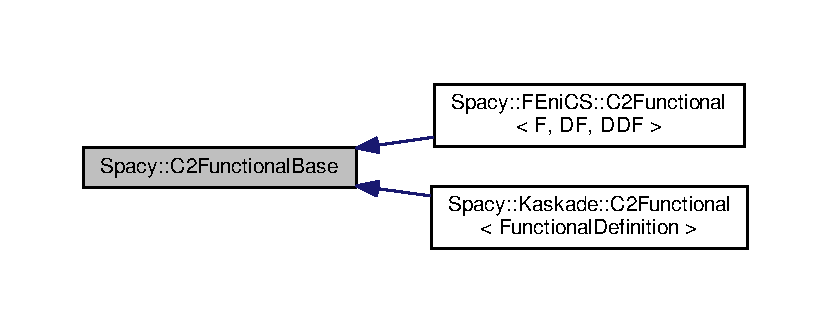
\includegraphics[width=350pt]{classSpacy_1_1C2FunctionalBase__inherit__graph}
\end{center}
\end{figure}
\subsection*{Public Member Functions}
\begin{DoxyCompactItemize}
\item 
\hyperlink{classSpacy_1_1C2FunctionalBase_a38ed7514896d9e7b576d22c12b6d153e_a38ed7514896d9e7b576d22c12b6d153e}{C2\+Functional\+Base} (const \hyperlink{classSpacy_1_1VectorSpace}{Vector\+Space} \&\hyperlink{classSpacy_1_1C2FunctionalBase_a016d11deb1525e762bdfbe7e54250718_a016d11deb1525e762bdfbe7e54250718}{domain})
\begin{DoxyCompactList}\small\item\em Constructor. \end{DoxyCompactList}\item 
const \hyperlink{classSpacy_1_1VectorSpace}{Vector\+Space} \& \hyperlink{classSpacy_1_1C2FunctionalBase_a016d11deb1525e762bdfbe7e54250718_a016d11deb1525e762bdfbe7e54250718}{domain} () const 
\begin{DoxyCompactList}\small\item\em Access domain space $X$. \end{DoxyCompactList}\end{DoxyCompactItemize}


\subsection{Detailed Description}
Base class for twice differentiable functionals $ f:\ X\rightarrow \mathbb{R}$. 

\subsection{Constructor \& Destructor Documentation}
\hypertarget{classSpacy_1_1C2FunctionalBase_a38ed7514896d9e7b576d22c12b6d153e_a38ed7514896d9e7b576d22c12b6d153e}{}\index{Spacy\+::\+C2\+Functional\+Base@{Spacy\+::\+C2\+Functional\+Base}!C2\+Functional\+Base@{C2\+Functional\+Base}}
\index{C2\+Functional\+Base@{C2\+Functional\+Base}!Spacy\+::\+C2\+Functional\+Base@{Spacy\+::\+C2\+Functional\+Base}}
\subsubsection[{C2\+Functional\+Base}]{\setlength{\rightskip}{0pt plus 5cm}Spacy\+::\+C2\+Functional\+Base\+::\+C2\+Functional\+Base (
\begin{DoxyParamCaption}
\item[{const {\bf Vector\+Space} \&}]{domain}
\end{DoxyParamCaption}
)\hspace{0.3cm}{\ttfamily [inline]}, {\ttfamily [explicit]}}\label{classSpacy_1_1C2FunctionalBase_a38ed7514896d9e7b576d22c12b6d153e_a38ed7514896d9e7b576d22c12b6d153e}


Constructor. 


\begin{DoxyParams}{Parameters}
{\em domain} & domain space $X$. \\
\hline
\end{DoxyParams}


\subsection{Member Function Documentation}
\hypertarget{classSpacy_1_1C2FunctionalBase_a016d11deb1525e762bdfbe7e54250718_a016d11deb1525e762bdfbe7e54250718}{}\index{Spacy\+::\+C2\+Functional\+Base@{Spacy\+::\+C2\+Functional\+Base}!domain@{domain}}
\index{domain@{domain}!Spacy\+::\+C2\+Functional\+Base@{Spacy\+::\+C2\+Functional\+Base}}
\subsubsection[{domain}]{\setlength{\rightskip}{0pt plus 5cm}const {\bf Vector\+Space}\& Spacy\+::\+C2\+Functional\+Base\+::domain (
\begin{DoxyParamCaption}
{}
\end{DoxyParamCaption}
) const\hspace{0.3cm}{\ttfamily [inline]}}\label{classSpacy_1_1C2FunctionalBase_a016d11deb1525e762bdfbe7e54250718_a016d11deb1525e762bdfbe7e54250718}


Access domain space $X$. 

\begin{DoxyReturn}{Returns}
domain space $X$. 
\end{DoxyReturn}


The documentation for this class was generated from the following file\+:\begin{DoxyCompactItemize}
\item 
Spacy/\+Util/\+Base/functional\+Base.\+hh\end{DoxyCompactItemize}

\hypertarget{classSpacy_1_1CallOfUndefinedFunctionException}{}\section{Spacy\+:\+:Call\+Of\+Undefined\+Function\+Exception Class Reference}
\label{classSpacy_1_1CallOfUndefinedFunctionException}\index{Spacy\+::\+Call\+Of\+Undefined\+Function\+Exception@{Spacy\+::\+Call\+Of\+Undefined\+Function\+Exception}}


Exception to be thrown if a virtual function is not implemented.  




{\ttfamily \#include $<$call\+Of\+Undefined\+Function\+Exception.\+hh$>$}



Inheritance diagram for Spacy\+:\+:Call\+Of\+Undefined\+Function\+Exception\+:\nopagebreak
\begin{figure}[H]
\begin{center}
\leavevmode
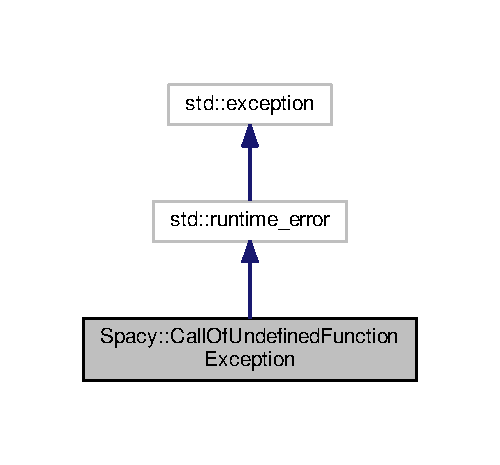
\includegraphics[width=240pt]{classSpacy_1_1CallOfUndefinedFunctionException__inherit__graph}
\end{center}
\end{figure}


Collaboration diagram for Spacy\+:\+:Call\+Of\+Undefined\+Function\+Exception\+:\nopagebreak
\begin{figure}[H]
\begin{center}
\leavevmode
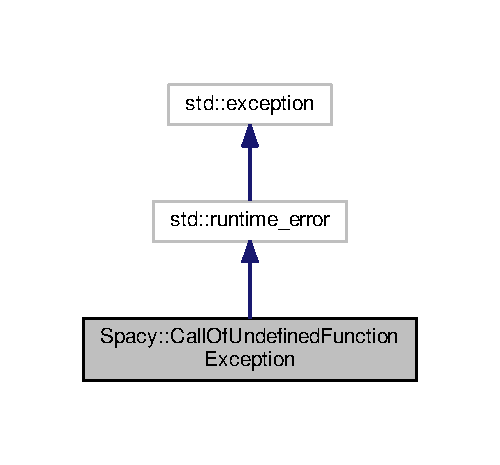
\includegraphics[width=240pt]{classSpacy_1_1CallOfUndefinedFunctionException__coll__graph}
\end{center}
\end{figure}
\subsection*{Public Member Functions}
\begin{DoxyCompactItemize}
\item 
\hyperlink{classSpacy_1_1CallOfUndefinedFunctionException_ac27ef399db59e2e21d91df93bc84f8c2_ac27ef399db59e2e21d91df93bc84f8c2}{Call\+Of\+Undefined\+Function\+Exception} (const std\+::string \&function)
\begin{DoxyCompactList}\small\item\em Constructor. \end{DoxyCompactList}\end{DoxyCompactItemize}


\subsection{Detailed Description}
Exception to be thrown if a virtual function is not implemented. 

\subsection{Constructor \& Destructor Documentation}
\hypertarget{classSpacy_1_1CallOfUndefinedFunctionException_ac27ef399db59e2e21d91df93bc84f8c2_ac27ef399db59e2e21d91df93bc84f8c2}{}\index{Spacy\+::\+Call\+Of\+Undefined\+Function\+Exception@{Spacy\+::\+Call\+Of\+Undefined\+Function\+Exception}!Call\+Of\+Undefined\+Function\+Exception@{Call\+Of\+Undefined\+Function\+Exception}}
\index{Call\+Of\+Undefined\+Function\+Exception@{Call\+Of\+Undefined\+Function\+Exception}!Spacy\+::\+Call\+Of\+Undefined\+Function\+Exception@{Spacy\+::\+Call\+Of\+Undefined\+Function\+Exception}}
\subsubsection[{Call\+Of\+Undefined\+Function\+Exception}]{\setlength{\rightskip}{0pt plus 5cm}Spacy\+::\+Call\+Of\+Undefined\+Function\+Exception\+::\+Call\+Of\+Undefined\+Function\+Exception (
\begin{DoxyParamCaption}
\item[{const std\+::string \&}]{function}
\end{DoxyParamCaption}
)}\label{classSpacy_1_1CallOfUndefinedFunctionException_ac27ef399db59e2e21d91df93bc84f8c2_ac27ef399db59e2e21d91df93bc84f8c2}


Constructor. 


\begin{DoxyParams}{Parameters}
{\em function} & name of function that throws \\
\hline
\end{DoxyParams}


The documentation for this class was generated from the following file\+:\begin{DoxyCompactItemize}
\item 
Spacy/\+Util/\+Exceptions/call\+Of\+Undefined\+Function\+Exception.\+hh\end{DoxyCompactItemize}

\hypertarget{classSpacy_1_1Mixin_1_1ContractionRate}{}\section{Spacy\+:\+:Mixin\+:\+:Contraction\+Rate Class Reference}
\label{classSpacy_1_1Mixin_1_1ContractionRate}\index{Spacy\+::\+Mixin\+::\+Contraction\+Rate@{Spacy\+::\+Mixin\+::\+Contraction\+Rate}}


Mixin class for contraction rates.  




{\ttfamily \#include $<$contraction\+Rate.\+hh$>$}



Inheritance diagram for Spacy\+:\+:Mixin\+:\+:Contraction\+Rate\+:\nopagebreak
\begin{figure}[H]
\begin{center}
\leavevmode
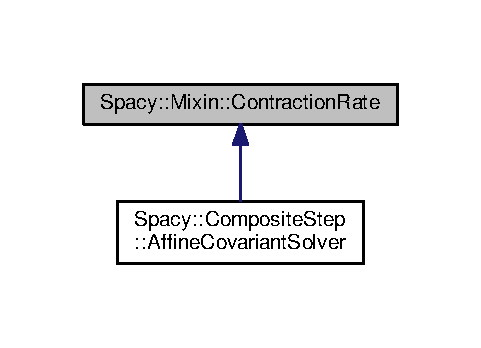
\includegraphics[width=231pt]{classSpacy_1_1Mixin_1_1ContractionRate__inherit__graph}
\end{center}
\end{figure}
\subsection*{Public Member Functions}
\begin{DoxyCompactItemize}
\item 
\hyperlink{classSpacy_1_1Mixin_1_1ContractionRate_a3d6b03823ce3951bafd51ceaac732bf7_a3d6b03823ce3951bafd51ceaac732bf7}{Contraction\+Rate} (\hyperlink{classSpacy_1_1Real}{Real} \hyperlink{classSpacy_1_1Mixin_1_1ContractionRate_aaefb97e44b51fb6c8017eb2b40659d64_aaefb97e44b51fb6c8017eb2b40659d64}{desired\+Contraction}=0.\+25, \hyperlink{classSpacy_1_1Real}{Real} \hyperlink{classSpacy_1_1Mixin_1_1ContractionRate_a569e3e3766394ccc46a13bd6ca122394_a569e3e3766394ccc46a13bd6ca122394}{relaxed\+Desired\+Contraction}=0.\+5, \hyperlink{classSpacy_1_1Real}{Real} \hyperlink{classSpacy_1_1Mixin_1_1ContractionRate_adea1388b1e492db1392f67cbe7e89302_adea1388b1e492db1392f67cbe7e89302}{maximal\+Contraction}=0.\+75) noexcept
\begin{DoxyCompactList}\small\item\em Constructor. \end{DoxyCompactList}\item 
void \hyperlink{classSpacy_1_1Mixin_1_1ContractionRate_ab9215981f0454bd5d641abad582e64e5_ab9215981f0454bd5d641abad582e64e5}{set\+Contraction} (\hyperlink{classSpacy_1_1Real}{Real} \hyperlink{classSpacy_1_1Mixin_1_1ContractionRate_a6c5e653393be91e468364733702e5334_a6c5e653393be91e468364733702e5334}{contraction}) noexcept
\begin{DoxyCompactList}\small\item\em Set contraction rate. \end{DoxyCompactList}\item 
void \hyperlink{classSpacy_1_1Mixin_1_1ContractionRate_a26eaa6344b5b2191931a9fd87ed96f39_a26eaa6344b5b2191931a9fd87ed96f39}{set\+Desired\+Contraction} (\hyperlink{classSpacy_1_1Real}{Real} \hyperlink{classSpacy_1_1Mixin_1_1ContractionRate_aaefb97e44b51fb6c8017eb2b40659d64_aaefb97e44b51fb6c8017eb2b40659d64}{desired\+Contraction}) noexcept
\begin{DoxyCompactList}\small\item\em Set desired contraction rate. \end{DoxyCompactList}\item 
void \hyperlink{classSpacy_1_1Mixin_1_1ContractionRate_ac6e47c0ab683643fea7490703f02632d_ac6e47c0ab683643fea7490703f02632d}{set\+Relaxed\+Desired\+Contraction} (\hyperlink{classSpacy_1_1Real}{Real} \hyperlink{classSpacy_1_1Mixin_1_1ContractionRate_a569e3e3766394ccc46a13bd6ca122394_a569e3e3766394ccc46a13bd6ca122394}{relaxed\+Desired\+Contraction}) noexcept
\begin{DoxyCompactList}\small\item\em Set relaxed desired contraction rate. \end{DoxyCompactList}\item 
void \hyperlink{classSpacy_1_1Mixin_1_1ContractionRate_acc99ba536cd9a027baa50a1412d9d216_acc99ba536cd9a027baa50a1412d9d216}{set\+Maximal\+Contraction} (\hyperlink{classSpacy_1_1Real}{Real} \hyperlink{classSpacy_1_1Mixin_1_1ContractionRate_adea1388b1e492db1392f67cbe7e89302_adea1388b1e492db1392f67cbe7e89302}{maximal\+Contraction}) noexcept
\begin{DoxyCompactList}\small\item\em Set maximal contraction rate. \end{DoxyCompactList}\item 
\hyperlink{classSpacy_1_1Real}{Real} \hyperlink{classSpacy_1_1Mixin_1_1ContractionRate_a6c5e653393be91e468364733702e5334_a6c5e653393be91e468364733702e5334}{contraction} () const noexcept
\begin{DoxyCompactList}\small\item\em Access contraction rate. \end{DoxyCompactList}\item 
\hyperlink{classSpacy_1_1Real}{Real} \hyperlink{classSpacy_1_1Mixin_1_1ContractionRate_aaefb97e44b51fb6c8017eb2b40659d64_aaefb97e44b51fb6c8017eb2b40659d64}{desired\+Contraction} () const noexcept
\begin{DoxyCompactList}\small\item\em Access desired contraction rate. \end{DoxyCompactList}\item 
\hyperlink{classSpacy_1_1Real}{Real} \hyperlink{classSpacy_1_1Mixin_1_1ContractionRate_a569e3e3766394ccc46a13bd6ca122394_a569e3e3766394ccc46a13bd6ca122394}{relaxed\+Desired\+Contraction} () const noexcept
\begin{DoxyCompactList}\small\item\em Get relaxed desired contraction rate. \end{DoxyCompactList}\item 
\hyperlink{classSpacy_1_1Real}{Real} \hyperlink{classSpacy_1_1Mixin_1_1ContractionRate_adea1388b1e492db1392f67cbe7e89302_adea1388b1e492db1392f67cbe7e89302}{maximal\+Contraction} () const noexcept
\begin{DoxyCompactList}\small\item\em Get desired contraction rate. \end{DoxyCompactList}\item 
bool \hyperlink{classSpacy_1_1Mixin_1_1ContractionRate_a7dd3c5eb5a7d14d8269207e3d1203aec_a7dd3c5eb5a7d14d8269207e3d1203aec}{admissible\+Contraction} () const noexcept
\begin{DoxyCompactList}\small\item\em Check if contraction is admissible. \end{DoxyCompactList}\end{DoxyCompactItemize}


\subsection{Detailed Description}
Mixin class for contraction rates. 

\subsection{Constructor \& Destructor Documentation}
\hypertarget{classSpacy_1_1Mixin_1_1ContractionRate_a3d6b03823ce3951bafd51ceaac732bf7_a3d6b03823ce3951bafd51ceaac732bf7}{}\index{Spacy\+::\+Mixin\+::\+Contraction\+Rate@{Spacy\+::\+Mixin\+::\+Contraction\+Rate}!Contraction\+Rate@{Contraction\+Rate}}
\index{Contraction\+Rate@{Contraction\+Rate}!Spacy\+::\+Mixin\+::\+Contraction\+Rate@{Spacy\+::\+Mixin\+::\+Contraction\+Rate}}
\subsubsection[{Contraction\+Rate}]{\setlength{\rightskip}{0pt plus 5cm}Spacy\+::\+Mixin\+::\+Contraction\+Rate\+::\+Contraction\+Rate (
\begin{DoxyParamCaption}
\item[{{\bf Real}}]{desired\+Contraction = {\ttfamily 0.25}, }
\item[{{\bf Real}}]{relaxed\+Desired\+Contraction = {\ttfamily 0.5}, }
\item[{{\bf Real}}]{maximal\+Contraction = {\ttfamily 0.75}}
\end{DoxyParamCaption}
)\hspace{0.3cm}{\ttfamily [explicit]}, {\ttfamily [noexcept]}}\label{classSpacy_1_1Mixin_1_1ContractionRate_a3d6b03823ce3951bafd51ceaac732bf7_a3d6b03823ce3951bafd51ceaac732bf7}


Constructor. 


\begin{DoxyParams}{Parameters}
{\em desired\+Contraction} & desired contraction rate \\
\hline
{\em relaxed\+Desired\+Contraction} & relaxed contraction rate \\
\hline
{\em maximal\+Contraction} & maximal allowed contraction rate \\
\hline
\end{DoxyParams}


\subsection{Member Function Documentation}
\hypertarget{classSpacy_1_1Mixin_1_1ContractionRate_a7dd3c5eb5a7d14d8269207e3d1203aec_a7dd3c5eb5a7d14d8269207e3d1203aec}{}\index{Spacy\+::\+Mixin\+::\+Contraction\+Rate@{Spacy\+::\+Mixin\+::\+Contraction\+Rate}!admissible\+Contraction@{admissible\+Contraction}}
\index{admissible\+Contraction@{admissible\+Contraction}!Spacy\+::\+Mixin\+::\+Contraction\+Rate@{Spacy\+::\+Mixin\+::\+Contraction\+Rate}}
\subsubsection[{admissible\+Contraction}]{\setlength{\rightskip}{0pt plus 5cm}bool Spacy\+::\+Mixin\+::\+Contraction\+Rate\+::admissible\+Contraction (
\begin{DoxyParamCaption}
{}
\end{DoxyParamCaption}
) const\hspace{0.3cm}{\ttfamily [noexcept]}}\label{classSpacy_1_1Mixin_1_1ContractionRate_a7dd3c5eb5a7d14d8269207e3d1203aec_a7dd3c5eb5a7d14d8269207e3d1203aec}


Check if contraction is admissible. 

\begin{DoxyReturn}{Returns}
\hyperlink{classSpacy_1_1Mixin_1_1ContractionRate_a6c5e653393be91e468364733702e5334_a6c5e653393be91e468364733702e5334}{contraction()} $<$ \hyperlink{classSpacy_1_1Mixin_1_1ContractionRate_adea1388b1e492db1392f67cbe7e89302_adea1388b1e492db1392f67cbe7e89302}{maximal\+Contraction()} 
\end{DoxyReturn}
\hypertarget{classSpacy_1_1Mixin_1_1ContractionRate_a6c5e653393be91e468364733702e5334_a6c5e653393be91e468364733702e5334}{}\index{Spacy\+::\+Mixin\+::\+Contraction\+Rate@{Spacy\+::\+Mixin\+::\+Contraction\+Rate}!contraction@{contraction}}
\index{contraction@{contraction}!Spacy\+::\+Mixin\+::\+Contraction\+Rate@{Spacy\+::\+Mixin\+::\+Contraction\+Rate}}
\subsubsection[{contraction}]{\setlength{\rightskip}{0pt plus 5cm}{\bf Real} Spacy\+::\+Mixin\+::\+Contraction\+Rate\+::contraction (
\begin{DoxyParamCaption}
{}
\end{DoxyParamCaption}
) const\hspace{0.3cm}{\ttfamily [noexcept]}}\label{classSpacy_1_1Mixin_1_1ContractionRate_a6c5e653393be91e468364733702e5334_a6c5e653393be91e468364733702e5334}


Access contraction rate. 

\begin{DoxyReturn}{Returns}
monitored contraction rate 
\end{DoxyReturn}
\hypertarget{classSpacy_1_1Mixin_1_1ContractionRate_aaefb97e44b51fb6c8017eb2b40659d64_aaefb97e44b51fb6c8017eb2b40659d64}{}\index{Spacy\+::\+Mixin\+::\+Contraction\+Rate@{Spacy\+::\+Mixin\+::\+Contraction\+Rate}!desired\+Contraction@{desired\+Contraction}}
\index{desired\+Contraction@{desired\+Contraction}!Spacy\+::\+Mixin\+::\+Contraction\+Rate@{Spacy\+::\+Mixin\+::\+Contraction\+Rate}}
\subsubsection[{desired\+Contraction}]{\setlength{\rightskip}{0pt plus 5cm}{\bf Real} Spacy\+::\+Mixin\+::\+Contraction\+Rate\+::desired\+Contraction (
\begin{DoxyParamCaption}
{}
\end{DoxyParamCaption}
) const\hspace{0.3cm}{\ttfamily [noexcept]}}\label{classSpacy_1_1Mixin_1_1ContractionRate_aaefb97e44b51fb6c8017eb2b40659d64_aaefb97e44b51fb6c8017eb2b40659d64}


Access desired contraction rate. 

\begin{DoxyReturn}{Returns}
desired contraction rate 
\end{DoxyReturn}
\hypertarget{classSpacy_1_1Mixin_1_1ContractionRate_adea1388b1e492db1392f67cbe7e89302_adea1388b1e492db1392f67cbe7e89302}{}\index{Spacy\+::\+Mixin\+::\+Contraction\+Rate@{Spacy\+::\+Mixin\+::\+Contraction\+Rate}!maximal\+Contraction@{maximal\+Contraction}}
\index{maximal\+Contraction@{maximal\+Contraction}!Spacy\+::\+Mixin\+::\+Contraction\+Rate@{Spacy\+::\+Mixin\+::\+Contraction\+Rate}}
\subsubsection[{maximal\+Contraction}]{\setlength{\rightskip}{0pt plus 5cm}{\bf Real} Spacy\+::\+Mixin\+::\+Contraction\+Rate\+::maximal\+Contraction (
\begin{DoxyParamCaption}
{}
\end{DoxyParamCaption}
) const\hspace{0.3cm}{\ttfamily [noexcept]}}\label{classSpacy_1_1Mixin_1_1ContractionRate_adea1388b1e492db1392f67cbe7e89302_adea1388b1e492db1392f67cbe7e89302}


Get desired contraction rate. 

\begin{DoxyReturn}{Returns}
maximal allowed contraction rate 
\end{DoxyReturn}
\hypertarget{classSpacy_1_1Mixin_1_1ContractionRate_a569e3e3766394ccc46a13bd6ca122394_a569e3e3766394ccc46a13bd6ca122394}{}\index{Spacy\+::\+Mixin\+::\+Contraction\+Rate@{Spacy\+::\+Mixin\+::\+Contraction\+Rate}!relaxed\+Desired\+Contraction@{relaxed\+Desired\+Contraction}}
\index{relaxed\+Desired\+Contraction@{relaxed\+Desired\+Contraction}!Spacy\+::\+Mixin\+::\+Contraction\+Rate@{Spacy\+::\+Mixin\+::\+Contraction\+Rate}}
\subsubsection[{relaxed\+Desired\+Contraction}]{\setlength{\rightskip}{0pt plus 5cm}{\bf Real} Spacy\+::\+Mixin\+::\+Contraction\+Rate\+::relaxed\+Desired\+Contraction (
\begin{DoxyParamCaption}
{}
\end{DoxyParamCaption}
) const\hspace{0.3cm}{\ttfamily [noexcept]}}\label{classSpacy_1_1Mixin_1_1ContractionRate_a569e3e3766394ccc46a13bd6ca122394_a569e3e3766394ccc46a13bd6ca122394}


Get relaxed desired contraction rate. 

\begin{DoxyReturn}{Returns}
relaxed contraction rate 
\end{DoxyReturn}
\hypertarget{classSpacy_1_1Mixin_1_1ContractionRate_ab9215981f0454bd5d641abad582e64e5_ab9215981f0454bd5d641abad582e64e5}{}\index{Spacy\+::\+Mixin\+::\+Contraction\+Rate@{Spacy\+::\+Mixin\+::\+Contraction\+Rate}!set\+Contraction@{set\+Contraction}}
\index{set\+Contraction@{set\+Contraction}!Spacy\+::\+Mixin\+::\+Contraction\+Rate@{Spacy\+::\+Mixin\+::\+Contraction\+Rate}}
\subsubsection[{set\+Contraction}]{\setlength{\rightskip}{0pt plus 5cm}void Spacy\+::\+Mixin\+::\+Contraction\+Rate\+::set\+Contraction (
\begin{DoxyParamCaption}
\item[{{\bf Real}}]{contraction}
\end{DoxyParamCaption}
)\hspace{0.3cm}{\ttfamily [noexcept]}}\label{classSpacy_1_1Mixin_1_1ContractionRate_ab9215981f0454bd5d641abad582e64e5_ab9215981f0454bd5d641abad582e64e5}


Set contraction rate. 


\begin{DoxyParams}{Parameters}
{\em contraction} & monitored contraction rate \\
\hline
\end{DoxyParams}
\hypertarget{classSpacy_1_1Mixin_1_1ContractionRate_a26eaa6344b5b2191931a9fd87ed96f39_a26eaa6344b5b2191931a9fd87ed96f39}{}\index{Spacy\+::\+Mixin\+::\+Contraction\+Rate@{Spacy\+::\+Mixin\+::\+Contraction\+Rate}!set\+Desired\+Contraction@{set\+Desired\+Contraction}}
\index{set\+Desired\+Contraction@{set\+Desired\+Contraction}!Spacy\+::\+Mixin\+::\+Contraction\+Rate@{Spacy\+::\+Mixin\+::\+Contraction\+Rate}}
\subsubsection[{set\+Desired\+Contraction}]{\setlength{\rightskip}{0pt plus 5cm}void Spacy\+::\+Mixin\+::\+Contraction\+Rate\+::set\+Desired\+Contraction (
\begin{DoxyParamCaption}
\item[{{\bf Real}}]{desired\+Contraction}
\end{DoxyParamCaption}
)\hspace{0.3cm}{\ttfamily [noexcept]}}\label{classSpacy_1_1Mixin_1_1ContractionRate_a26eaa6344b5b2191931a9fd87ed96f39_a26eaa6344b5b2191931a9fd87ed96f39}


Set desired contraction rate. 


\begin{DoxyParams}{Parameters}
{\em desired\+Contraction} & desired contraction rate \\
\hline
\end{DoxyParams}
\hypertarget{classSpacy_1_1Mixin_1_1ContractionRate_acc99ba536cd9a027baa50a1412d9d216_acc99ba536cd9a027baa50a1412d9d216}{}\index{Spacy\+::\+Mixin\+::\+Contraction\+Rate@{Spacy\+::\+Mixin\+::\+Contraction\+Rate}!set\+Maximal\+Contraction@{set\+Maximal\+Contraction}}
\index{set\+Maximal\+Contraction@{set\+Maximal\+Contraction}!Spacy\+::\+Mixin\+::\+Contraction\+Rate@{Spacy\+::\+Mixin\+::\+Contraction\+Rate}}
\subsubsection[{set\+Maximal\+Contraction}]{\setlength{\rightskip}{0pt plus 5cm}void Spacy\+::\+Mixin\+::\+Contraction\+Rate\+::set\+Maximal\+Contraction (
\begin{DoxyParamCaption}
\item[{{\bf Real}}]{maximal\+Contraction}
\end{DoxyParamCaption}
)\hspace{0.3cm}{\ttfamily [noexcept]}}\label{classSpacy_1_1Mixin_1_1ContractionRate_acc99ba536cd9a027baa50a1412d9d216_acc99ba536cd9a027baa50a1412d9d216}


Set maximal contraction rate. 


\begin{DoxyParams}{Parameters}
{\em maximal\+Contraction} & maximal allowed contraction rate \\
\hline
\end{DoxyParams}
\hypertarget{classSpacy_1_1Mixin_1_1ContractionRate_ac6e47c0ab683643fea7490703f02632d_ac6e47c0ab683643fea7490703f02632d}{}\index{Spacy\+::\+Mixin\+::\+Contraction\+Rate@{Spacy\+::\+Mixin\+::\+Contraction\+Rate}!set\+Relaxed\+Desired\+Contraction@{set\+Relaxed\+Desired\+Contraction}}
\index{set\+Relaxed\+Desired\+Contraction@{set\+Relaxed\+Desired\+Contraction}!Spacy\+::\+Mixin\+::\+Contraction\+Rate@{Spacy\+::\+Mixin\+::\+Contraction\+Rate}}
\subsubsection[{set\+Relaxed\+Desired\+Contraction}]{\setlength{\rightskip}{0pt plus 5cm}void Spacy\+::\+Mixin\+::\+Contraction\+Rate\+::set\+Relaxed\+Desired\+Contraction (
\begin{DoxyParamCaption}
\item[{{\bf Real}}]{relaxed\+Desired\+Contraction}
\end{DoxyParamCaption}
)\hspace{0.3cm}{\ttfamily [noexcept]}}\label{classSpacy_1_1Mixin_1_1ContractionRate_ac6e47c0ab683643fea7490703f02632d_ac6e47c0ab683643fea7490703f02632d}


Set relaxed desired contraction rate. 


\begin{DoxyParams}{Parameters}
{\em relaxed\+Desired\+Contraction} & relaxed contraction rate \\
\hline
\end{DoxyParams}


The documentation for this class was generated from the following file\+:\begin{DoxyCompactItemize}
\item 
Spacy/\+Util/\+Mixins/contraction\+Rate.\+hh\end{DoxyCompactItemize}

\hypertarget{classSpacy_1_1Mixin_1_1ControlIndex}{}\section{Spacy\+:\+:Mixin\+:\+:Control\+Index Class Reference}
\label{classSpacy_1_1Mixin_1_1ControlIndex}\index{Spacy\+::\+Mixin\+::\+Control\+Index@{Spacy\+::\+Mixin\+::\+Control\+Index}}


Mixin class for index of the control variable.  




{\ttfamily \#include $<$control\+Index.\+hh$>$}



Inheritance diagram for Spacy\+:\+:Mixin\+:\+:Control\+Index\+:\nopagebreak
\begin{figure}[H]
\begin{center}
\leavevmode
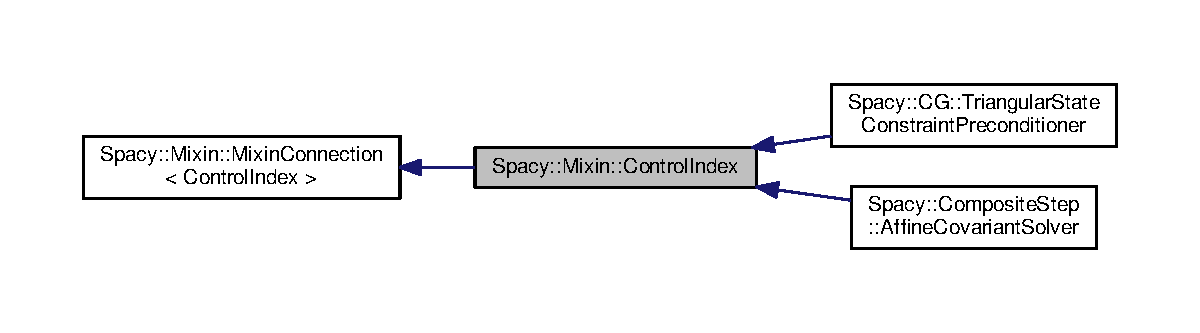
\includegraphics[width=350pt]{classSpacy_1_1Mixin_1_1ControlIndex__inherit__graph}
\end{center}
\end{figure}


Collaboration diagram for Spacy\+:\+:Mixin\+:\+:Control\+Index\+:\nopagebreak
\begin{figure}[H]
\begin{center}
\leavevmode
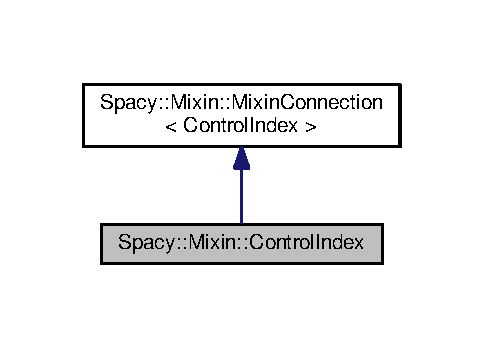
\includegraphics[width=232pt]{classSpacy_1_1Mixin_1_1ControlIndex__coll__graph}
\end{center}
\end{figure}
\subsection*{Public Member Functions}
\begin{DoxyCompactItemize}
\item 
\hypertarget{classSpacy_1_1Mixin_1_1ControlIndex_afa09ff1cc2b7476e8b6e7e26e71cd775}{}{\bfseries Control\+Index} (unsigned index=1) noexcept\label{classSpacy_1_1Mixin_1_1ControlIndex_afa09ff1cc2b7476e8b6e7e26e71cd775}

\item 
\hypertarget{classSpacy_1_1Mixin_1_1ControlIndex_a4e6c305c148d81f15638fc214f60ed00}{}void {\bfseries set\+Control\+Index} (unsigned index)\label{classSpacy_1_1Mixin_1_1ControlIndex_a4e6c305c148d81f15638fc214f60ed00}

\item 
\hypertarget{classSpacy_1_1Mixin_1_1ControlIndex_a04fd74c67e320942ff6513fe0a741913}{}double {\bfseries control\+Index} () const noexcept\label{classSpacy_1_1Mixin_1_1ControlIndex_a04fd74c67e320942ff6513fe0a741913}

\item 
\hypertarget{classSpacy_1_1Mixin_1_1ControlIndex_aa534a05629e88a5cc479f161139cf3f7}{}void \hyperlink{classSpacy_1_1Mixin_1_1ControlIndex_aa534a05629e88a5cc479f161139cf3f7}{update} (\hyperlink{classSpacy_1_1Mixin_1_1ControlIndex}{Control\+Index} $\ast$changed\+Subject)\label{classSpacy_1_1Mixin_1_1ControlIndex_aa534a05629e88a5cc479f161139cf3f7}

\begin{DoxyCompactList}\small\item\em update function for observer pattern. \end{DoxyCompactList}\item 
\hypertarget{classSpacy_1_1Mixin_1_1MixinConnection_abb5520ee6b22dd993d78f142939a1ed4}{}void \hyperlink{classSpacy_1_1Mixin_1_1MixinConnection_abb5520ee6b22dd993d78f142939a1ed4}{attach} (\hyperlink{classSpacy_1_1Mixin_1_1ControlIndex}{Control\+Index} \&observer)\label{classSpacy_1_1Mixin_1_1MixinConnection_abb5520ee6b22dd993d78f142939a1ed4}

\begin{DoxyCompactList}\small\item\em Attach observer. \end{DoxyCompactList}\item 
\hypertarget{classSpacy_1_1Mixin_1_1MixinConnection_adda739590c487679c26f60e50aedb73f}{}void \hyperlink{classSpacy_1_1Mixin_1_1MixinConnection_adda739590c487679c26f60e50aedb73f}{detach} (\hyperlink{classSpacy_1_1Mixin_1_1ControlIndex}{Control\+Index} \&observer)\label{classSpacy_1_1Mixin_1_1MixinConnection_adda739590c487679c26f60e50aedb73f}

\begin{DoxyCompactList}\small\item\em Detach observer. \end{DoxyCompactList}\item 
\hypertarget{classSpacy_1_1Mixin_1_1MixinConnection_a1ddeaa78a3bb4a38c2cca36d1f99fe36}{}void \hyperlink{classSpacy_1_1Mixin_1_1MixinConnection_a1ddeaa78a3bb4a38c2cca36d1f99fe36}{notify} ()\label{classSpacy_1_1Mixin_1_1MixinConnection_a1ddeaa78a3bb4a38c2cca36d1f99fe36}

\begin{DoxyCompactList}\small\item\em Notify observers about changes. \end{DoxyCompactList}\end{DoxyCompactItemize}


\subsection{Detailed Description}
Mixin class for index of the control variable. 

The documentation for this class was generated from the following file\+:\begin{DoxyCompactItemize}
\item 
Spacy/\+Util/\+Mixins/control\+Index.\+hh\end{DoxyCompactItemize}

\hypertarget{classSpacy_1_1Mixin_1_1CopyingUniqueImpl}{}\section{Spacy\+:\+:Mixin\+:\+:Copying\+Unique\+Impl$<$ Type $>$ Class Template Reference}
\label{classSpacy_1_1Mixin_1_1CopyingUniqueImpl}\index{Spacy\+::\+Mixin\+::\+Copying\+Unique\+Impl$<$ Type $>$@{Spacy\+::\+Mixin\+::\+Copying\+Unique\+Impl$<$ Type $>$}}


Stores an object of type Type as unique pointer and provides access via member function \hyperlink{classSpacy_1_1Mixin_1_1CopyingUniqueImpl_ab7cc202fd000ba1753ef8596c09dc803}{impl()}.  




{\ttfamily \#include $<$impl.\+hh$>$}

\subsection*{Public Member Functions}
\begin{DoxyCompactItemize}
\item 
\hypertarget{classSpacy_1_1Mixin_1_1CopyingUniqueImpl_ad0fc9e321b82e636f0859df171142a01}{}\hyperlink{classSpacy_1_1Mixin_1_1CopyingUniqueImpl_ad0fc9e321b82e636f0859df171142a01}{Copying\+Unique\+Impl} ()=default\label{classSpacy_1_1Mixin_1_1CopyingUniqueImpl_ad0fc9e321b82e636f0859df171142a01}

\begin{DoxyCompactList}\small\item\em Default constructor. \end{DoxyCompactList}\item 
\hyperlink{classSpacy_1_1Mixin_1_1CopyingUniqueImpl_aae94252db5d9b1b13ad62cbe2fcd6086_aae94252db5d9b1b13ad62cbe2fcd6086}{Copying\+Unique\+Impl} (std\+::unique\+\_\+ptr$<$ Type $>$ \&\&\hyperlink{classSpacy_1_1Mixin_1_1CopyingUniqueImpl_ab7cc202fd000ba1753ef8596c09dc803}{impl})
\begin{DoxyCompactList}\small\item\em Constructor. \end{DoxyCompactList}\item 
\hypertarget{classSpacy_1_1Mixin_1_1CopyingUniqueImpl_a6d84fb0932af2d3f8015fae16627f37d}{}{\bfseries Copying\+Unique\+Impl} (const \hyperlink{classSpacy_1_1Mixin_1_1CopyingUniqueImpl}{Copying\+Unique\+Impl} \&other)\label{classSpacy_1_1Mixin_1_1CopyingUniqueImpl_a6d84fb0932af2d3f8015fae16627f37d}

\item 
\hypertarget{classSpacy_1_1Mixin_1_1CopyingUniqueImpl_a85a1b465406461ce461e7e67336a72d7}{}\hyperlink{classSpacy_1_1Mixin_1_1CopyingUniqueImpl}{Copying\+Unique\+Impl} \& {\bfseries operator=} (const \hyperlink{classSpacy_1_1Mixin_1_1CopyingUniqueImpl}{Copying\+Unique\+Impl} \&other)\label{classSpacy_1_1Mixin_1_1CopyingUniqueImpl_a85a1b465406461ce461e7e67336a72d7}

\item 
\hypertarget{classSpacy_1_1Mixin_1_1CopyingUniqueImpl_a513e88451b85b40b9f0ac0012e5adf41}{}{\bfseries Copying\+Unique\+Impl} (\hyperlink{classSpacy_1_1Mixin_1_1CopyingUniqueImpl}{Copying\+Unique\+Impl} \&\&)=default\label{classSpacy_1_1Mixin_1_1CopyingUniqueImpl_a513e88451b85b40b9f0ac0012e5adf41}

\item 
\hypertarget{classSpacy_1_1Mixin_1_1CopyingUniqueImpl_a9f79e3b36b5df2be63025629213dc9d7}{}\hyperlink{classSpacy_1_1Mixin_1_1CopyingUniqueImpl}{Copying\+Unique\+Impl} \& {\bfseries operator=} (\hyperlink{classSpacy_1_1Mixin_1_1CopyingUniqueImpl}{Copying\+Unique\+Impl} \&\&other)\label{classSpacy_1_1Mixin_1_1CopyingUniqueImpl_a9f79e3b36b5df2be63025629213dc9d7}

\item 
\hypertarget{classSpacy_1_1Mixin_1_1CopyingUniqueImpl_ab7cc202fd000ba1753ef8596c09dc803}{}Type \& \hyperlink{classSpacy_1_1Mixin_1_1CopyingUniqueImpl_ab7cc202fd000ba1753ef8596c09dc803}{impl} ()\label{classSpacy_1_1Mixin_1_1CopyingUniqueImpl_ab7cc202fd000ba1753ef8596c09dc803}

\begin{DoxyCompactList}\small\item\em Access implementation. \end{DoxyCompactList}\item 
\hypertarget{classSpacy_1_1Mixin_1_1CopyingUniqueImpl_a6bdd26b4d36f442aa606a9e65d41c71c}{}const Type \& \hyperlink{classSpacy_1_1Mixin_1_1CopyingUniqueImpl_a6bdd26b4d36f442aa606a9e65d41c71c}{impl} () const \label{classSpacy_1_1Mixin_1_1CopyingUniqueImpl_a6bdd26b4d36f442aa606a9e65d41c71c}

\begin{DoxyCompactList}\small\item\em Access implementation. \end{DoxyCompactList}\item 
\hypertarget{classSpacy_1_1Mixin_1_1CopyingUniqueImpl_aaa5b34c44e72ae4fe0d7f283d67600d0}{}bool \hyperlink{classSpacy_1_1Mixin_1_1CopyingUniqueImpl_aaa5b34c44e72ae4fe0d7f283d67600d0}{impl\+Is\+Null\+Ptr} () const \label{classSpacy_1_1Mixin_1_1CopyingUniqueImpl_aaa5b34c44e72ae4fe0d7f283d67600d0}

\begin{DoxyCompactList}\small\item\em Check if stored object is null pointer. \end{DoxyCompactList}\end{DoxyCompactItemize}


\subsection{Detailed Description}
\subsubsection*{template$<$class Type$>$class Spacy\+::\+Mixin\+::\+Copying\+Unique\+Impl$<$ Type $>$}

Stores an object of type Type as unique pointer and provides access via member function \hyperlink{classSpacy_1_1Mixin_1_1CopyingUniqueImpl_ab7cc202fd000ba1753ef8596c09dc803}{impl()}. 

\subsection{Constructor \& Destructor Documentation}
\hypertarget{classSpacy_1_1Mixin_1_1CopyingUniqueImpl_aae94252db5d9b1b13ad62cbe2fcd6086_aae94252db5d9b1b13ad62cbe2fcd6086}{}\index{Spacy\+::\+Mixin\+::\+Copying\+Unique\+Impl@{Spacy\+::\+Mixin\+::\+Copying\+Unique\+Impl}!Copying\+Unique\+Impl@{Copying\+Unique\+Impl}}
\index{Copying\+Unique\+Impl@{Copying\+Unique\+Impl}!Spacy\+::\+Mixin\+::\+Copying\+Unique\+Impl@{Spacy\+::\+Mixin\+::\+Copying\+Unique\+Impl}}
\subsubsection[{Copying\+Unique\+Impl}]{\setlength{\rightskip}{0pt plus 5cm}template$<$class Type$>$ {\bf Spacy\+::\+Mixin\+::\+Copying\+Unique\+Impl}$<$ Type $>$\+::{\bf Copying\+Unique\+Impl} (
\begin{DoxyParamCaption}
\item[{std\+::unique\+\_\+ptr$<$ Type $>$ \&\&}]{impl}
\end{DoxyParamCaption}
)\hspace{0.3cm}{\ttfamily [inline]}, {\ttfamily [explicit]}}\label{classSpacy_1_1Mixin_1_1CopyingUniqueImpl_aae94252db5d9b1b13ad62cbe2fcd6086_aae94252db5d9b1b13ad62cbe2fcd6086}


Constructor. 


\begin{DoxyParams}{Parameters}
{\em impl} & value to be stored. \\
\hline
\end{DoxyParams}


The documentation for this class was generated from the following file\+:\begin{DoxyCompactItemize}
\item 
Spacy/\+Util/\+Mixins/impl.\+hh\end{DoxyCompactItemize}

\hypertarget{classSpacy_1_1Functions__1D_1_1Cubic}{}\section{Spacy\+:\+:Functions\+\_\+1\+D\+:\+:Cubic Class Reference}
\label{classSpacy_1_1Functions__1D_1_1Cubic}\index{Spacy\+::\+Functions\+\_\+1\+D\+::\+Cubic@{Spacy\+::\+Functions\+\_\+1\+D\+::\+Cubic}}


A one-\/dimensional cubic function $q(t) = a + bt + ct^2 + dt^3$.  




{\ttfamily \#include $<$cubic.\+hh$>$}

\subsection*{Public Member Functions}
\begin{DoxyCompactItemize}
\item 
\hypertarget{classSpacy_1_1Functions__1D_1_1Cubic_a02138df0eb7552a66c4d4c4ab1e23771}{}{\bfseries Cubic} (\hyperlink{classSpacy_1_1Real}{Real} a, \hyperlink{classSpacy_1_1Real}{Real} b, \hyperlink{classSpacy_1_1Real}{Real} c, \hyperlink{classSpacy_1_1Real}{Real} d) noexcept\label{classSpacy_1_1Functions__1D_1_1Cubic_a02138df0eb7552a66c4d4c4ab1e23771}

\item 
\hypertarget{classSpacy_1_1Functions__1D_1_1Cubic_adeb72297c0849ada705f61dbe0f1ea61}{}\hyperlink{classSpacy_1_1Real}{Real} \hyperlink{classSpacy_1_1Functions__1D_1_1Cubic_adeb72297c0849ada705f61dbe0f1ea61}{operator()} (\hyperlink{classSpacy_1_1Real}{Real} t) const noexcept\label{classSpacy_1_1Functions__1D_1_1Cubic_adeb72297c0849ada705f61dbe0f1ea61}

\begin{DoxyCompactList}\small\item\em Compute $q(t) = a + bt + ct^2 + dt^3 $. \end{DoxyCompactList}\end{DoxyCompactItemize}


\subsection{Detailed Description}
A one-\/dimensional cubic function $q(t) = a + bt + ct^2 + dt^3$. 

The documentation for this class was generated from the following file\+:\begin{DoxyCompactItemize}
\item 
Spacy/\+Algorithm/\+Functions\+\_\+1\+D/cubic.\+hh\end{DoxyCompactItemize}

\hypertarget{classSpacy_1_1CompositeStep_1_1CubicModel}{}\section{Spacy\+:\+:Composite\+Step\+:\+:Cubic\+Model Class Reference}
\label{classSpacy_1_1CompositeStep_1_1CubicModel}\index{Spacy\+::\+Composite\+Step\+::\+Cubic\+Model@{Spacy\+::\+Composite\+Step\+::\+Cubic\+Model}}


The cubic regularized model for Affine\+Covariant\+Composite\+Steps.  




{\ttfamily \#include $<$quadratic\+Model.\+hh$>$}

\subsection*{Public Member Functions}
\begin{DoxyCompactItemize}
\item 
\hyperlink{classSpacy_1_1CompositeStep_1_1CubicModel_abbae58ccfdd50120fc10245251048b91_abbae58ccfdd50120fc10245251048b91}{Cubic\+Model} (const \hyperlink{classSpacy_1_1Functions__1D_1_1Quadratic}{Functions\+\_\+1\+D\+::\+Quadratic} \&quadratic\+Model, const \hyperlink{classSpacy_1_1Functions__1D_1_1Quadratic}{Functions\+\_\+1\+D\+::\+Quadratic} \&squared\+Norm, \hyperlink{classSpacy_1_1Real}{Real} omega)
\begin{DoxyCompactList}\small\item\em Constructor. \end{DoxyCompactList}\item 
\hyperlink{classSpacy_1_1Real}{Real} \hyperlink{classSpacy_1_1CompositeStep_1_1CubicModel_a5669f387117cfdc47b5be45a29f387ce_a5669f387117cfdc47b5be45a29f387ce}{operator()} (\hyperlink{classSpacy_1_1Real}{Real} t) const 
\begin{DoxyCompactList}\small\item\em Evaluate cubic model $ q(t) = q_1(t) + \frac{\omega}{6}q_2^{3/2} $. \end{DoxyCompactList}\end{DoxyCompactItemize}


\subsection{Detailed Description}
The cubic regularized model for Affine\+Covariant\+Composite\+Steps. 

\subsection{Constructor \& Destructor Documentation}
\hypertarget{classSpacy_1_1CompositeStep_1_1CubicModel_abbae58ccfdd50120fc10245251048b91_abbae58ccfdd50120fc10245251048b91}{}\index{Spacy\+::\+Composite\+Step\+::\+Cubic\+Model@{Spacy\+::\+Composite\+Step\+::\+Cubic\+Model}!Cubic\+Model@{Cubic\+Model}}
\index{Cubic\+Model@{Cubic\+Model}!Spacy\+::\+Composite\+Step\+::\+Cubic\+Model@{Spacy\+::\+Composite\+Step\+::\+Cubic\+Model}}
\subsubsection[{Cubic\+Model}]{\setlength{\rightskip}{0pt plus 5cm}Spacy\+::\+Composite\+Step\+::\+Cubic\+Model\+::\+Cubic\+Model (
\begin{DoxyParamCaption}
\item[{const {\bf Functions\+\_\+1\+D\+::\+Quadratic} \&}]{quadratic\+Model, }
\item[{const {\bf Functions\+\_\+1\+D\+::\+Quadratic} \&}]{squared\+Norm, }
\item[{{\bf Real}}]{omega}
\end{DoxyParamCaption}
)}\label{classSpacy_1_1CompositeStep_1_1CubicModel_abbae58ccfdd50120fc10245251048b91_abbae58ccfdd50120fc10245251048b91}


Constructor. 


\begin{DoxyParams}{Parameters}
{\em quadratic\+Model} & quadratic model $q_1$ of the Lagrange functional (generated with make\+Quadratic\+Model(...)) \\
\hline
{\em squared\+Norm} & quadratic model $q_2$ of a norm (generated with make\+Quadratic\+Norm\+Model(...)) \\
\hline
{\em omega} & estimate of the Lipschitz constant of the second derivative of the Lagrangian \\
\hline
\end{DoxyParams}


\subsection{Member Function Documentation}
\hypertarget{classSpacy_1_1CompositeStep_1_1CubicModel_a5669f387117cfdc47b5be45a29f387ce_a5669f387117cfdc47b5be45a29f387ce}{}\index{Spacy\+::\+Composite\+Step\+::\+Cubic\+Model@{Spacy\+::\+Composite\+Step\+::\+Cubic\+Model}!operator()@{operator()}}
\index{operator()@{operator()}!Spacy\+::\+Composite\+Step\+::\+Cubic\+Model@{Spacy\+::\+Composite\+Step\+::\+Cubic\+Model}}
\subsubsection[{operator()}]{\setlength{\rightskip}{0pt plus 5cm}{\bf Real} Spacy\+::\+Composite\+Step\+::\+Cubic\+Model\+::operator() (
\begin{DoxyParamCaption}
\item[{{\bf Real}}]{t}
\end{DoxyParamCaption}
) const}\label{classSpacy_1_1CompositeStep_1_1CubicModel_a5669f387117cfdc47b5be45a29f387ce_a5669f387117cfdc47b5be45a29f387ce}


Evaluate cubic model $ q(t) = q_1(t) + \frac{\omega}{6}q_2^{3/2} $. 


\begin{DoxyParams}{Parameters}
{\em t} & argument \\
\hline
\end{DoxyParams}
\begin{DoxyReturn}{Returns}
$ q(t) = q_1(t) + \frac{\omega}{6}q_2^{3/2} $ 
\end{DoxyReturn}


The documentation for this class was generated from the following file\+:\begin{DoxyCompactItemize}
\item 
Spacy/\+Algorithm/\+Composite\+Step/quadratic\+Model.\+hh\end{DoxyCompactItemize}

\hypertarget{structSpacy_1_1Kaskade_1_1ErrorDistribution_1_1D1}{}\section{Spacy\+:\+:Kaskade\+:\+:Error\+Distribution$<$ Functional, Extended\+Ansatz\+Vars $>$\+:\+:D1$<$ row $>$ Struct Template Reference}
\label{structSpacy_1_1Kaskade_1_1ErrorDistribution_1_1D1}\index{Spacy\+::\+Kaskade\+::\+Error\+Distribution$<$ Functional, Extended\+Ansatz\+Vars $>$\+::\+D1$<$ row $>$@{Spacy\+::\+Kaskade\+::\+Error\+Distribution$<$ Functional, Extended\+Ansatz\+Vars $>$\+::\+D1$<$ row $>$}}


Inheritance diagram for Spacy\+:\+:Kaskade\+:\+:Error\+Distribution$<$ Functional, Extended\+Ansatz\+Vars $>$\+:\+:D1$<$ row $>$\+:\nopagebreak
\begin{figure}[H]
\begin{center}
\leavevmode
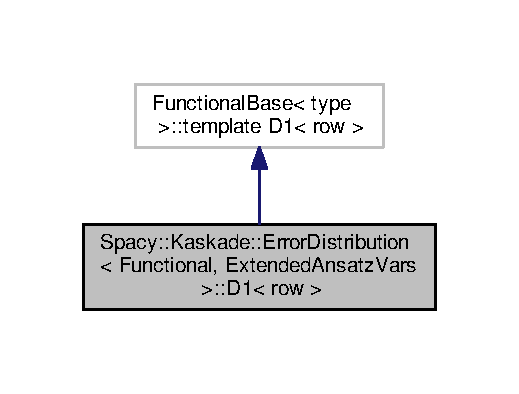
\includegraphics[width=249pt]{structSpacy_1_1Kaskade_1_1ErrorDistribution_1_1D1__inherit__graph}
\end{center}
\end{figure}


Collaboration diagram for Spacy\+:\+:Kaskade\+:\+:Error\+Distribution$<$ Functional, Extended\+Ansatz\+Vars $>$\+:\+:D1$<$ row $>$\+:\nopagebreak
\begin{figure}[H]
\begin{center}
\leavevmode
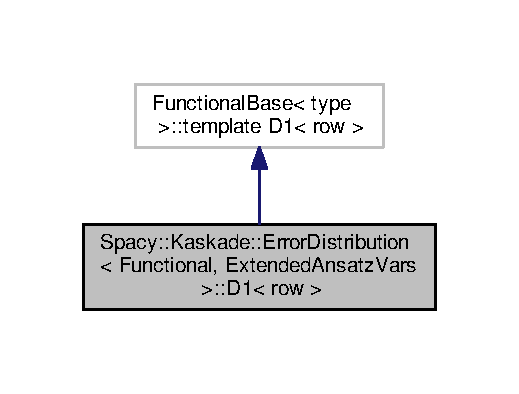
\includegraphics[width=249pt]{structSpacy_1_1Kaskade_1_1ErrorDistribution_1_1D1__coll__graph}
\end{center}
\end{figure}
\subsection*{Static Public Attributes}
\begin{DoxyCompactItemize}
\item 
\hypertarget{structSpacy_1_1Kaskade_1_1ErrorDistribution_1_1D1_ae12f3e44e152e93d2855a893a436472f}{}static bool const {\bfseries present} = true\label{structSpacy_1_1Kaskade_1_1ErrorDistribution_1_1D1_ae12f3e44e152e93d2855a893a436472f}

\item 
\hypertarget{structSpacy_1_1Kaskade_1_1ErrorDistribution_1_1D1_aebe5d1ff61fe5bd5274fd440ebeccfb5}{}static bool const {\bfseries constant} = false\label{structSpacy_1_1Kaskade_1_1ErrorDistribution_1_1D1_aebe5d1ff61fe5bd5274fd440ebeccfb5}

\end{DoxyCompactItemize}


The documentation for this struct was generated from the following file\+:\begin{DoxyCompactItemize}
\item 
Spacy/\+Adapter/\+Kaskade/\+Definitions/error\+\_\+distribution.\+hh\end{DoxyCompactItemize}

\hypertarget{structSpacy_1_1Kaskade_1_1ErrorDistribution_1_1D2}{}\section{Spacy\+:\+:Kaskade\+:\+:Error\+Distribution$<$ Functional, Extended\+Ansatz\+Vars $>$\+:\+:D2$<$ row, col $>$ Struct Template Reference}
\label{structSpacy_1_1Kaskade_1_1ErrorDistribution_1_1D2}\index{Spacy\+::\+Kaskade\+::\+Error\+Distribution$<$ Functional, Extended\+Ansatz\+Vars $>$\+::\+D2$<$ row, col $>$@{Spacy\+::\+Kaskade\+::\+Error\+Distribution$<$ Functional, Extended\+Ansatz\+Vars $>$\+::\+D2$<$ row, col $>$}}


Inheritance diagram for Spacy\+:\+:Kaskade\+:\+:Error\+Distribution$<$ Functional, Extended\+Ansatz\+Vars $>$\+:\+:D2$<$ row, col $>$\+:\nopagebreak
\begin{figure}[H]
\begin{center}
\leavevmode
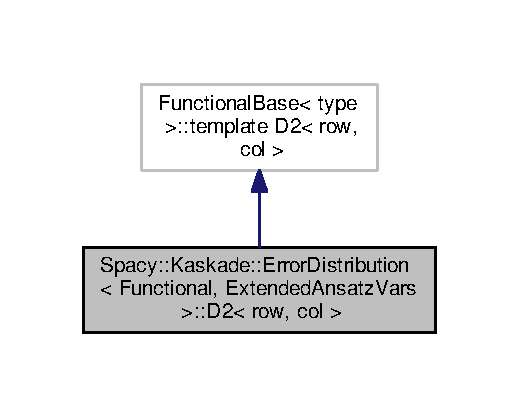
\includegraphics[width=249pt]{structSpacy_1_1Kaskade_1_1ErrorDistribution_1_1D2__inherit__graph}
\end{center}
\end{figure}


Collaboration diagram for Spacy\+:\+:Kaskade\+:\+:Error\+Distribution$<$ Functional, Extended\+Ansatz\+Vars $>$\+:\+:D2$<$ row, col $>$\+:\nopagebreak
\begin{figure}[H]
\begin{center}
\leavevmode
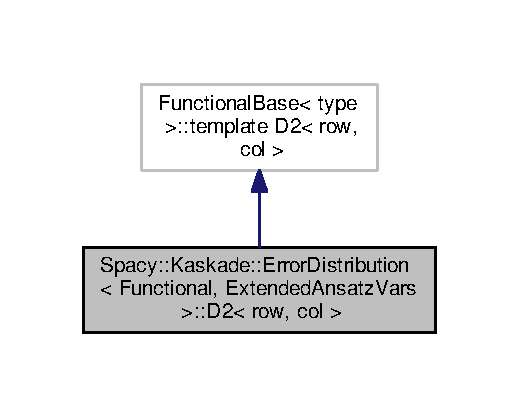
\includegraphics[width=249pt]{structSpacy_1_1Kaskade_1_1ErrorDistribution_1_1D2__coll__graph}
\end{center}
\end{figure}
\subsection*{Static Public Attributes}
\begin{DoxyCompactItemize}
\item 
\hypertarget{structSpacy_1_1Kaskade_1_1ErrorDistribution_1_1D2_a527d46a4da6e1ddf997e2d91837cd0b3}{}static bool const {\bfseries present} = false\label{structSpacy_1_1Kaskade_1_1ErrorDistribution_1_1D2_a527d46a4da6e1ddf997e2d91837cd0b3}

\item 
\hypertarget{structSpacy_1_1Kaskade_1_1ErrorDistribution_1_1D2_af11aed2f092b490a062402d1966f4f8f}{}static bool const {\bfseries symmetric} = false\label{structSpacy_1_1Kaskade_1_1ErrorDistribution_1_1D2_af11aed2f092b490a062402d1966f4f8f}

\item 
\hypertarget{structSpacy_1_1Kaskade_1_1ErrorDistribution_1_1D2_af140ebc24432aef6ad4aabccfe0b359d}{}static bool const {\bfseries lumped} = false\label{structSpacy_1_1Kaskade_1_1ErrorDistribution_1_1D2_af140ebc24432aef6ad4aabccfe0b359d}

\end{DoxyCompactItemize}


The documentation for this struct was generated from the following file\+:\begin{DoxyCompactItemize}
\item 
Spacy/\+Adapter/\+Kaskade/\+Definitions/error\+\_\+distribution.\+hh\end{DoxyCompactItemize}

\hypertarget{classSpacy_1_1Mixin_1_1DampingAccuracy}{}\section{Spacy\+:\+:Mixin\+:\+:Damping\+Accuracy Class Reference}
\label{classSpacy_1_1Mixin_1_1DampingAccuracy}\index{Spacy\+::\+Mixin\+::\+Damping\+Accuracy@{Spacy\+::\+Mixin\+::\+Damping\+Accuracy}}


Mixin class for the accuracy of damping factors.  




{\ttfamily \#include $<$damping\+Accuracy.\+hh$>$}



Inheritance diagram for Spacy\+:\+:Mixin\+:\+:Damping\+Accuracy\+:\nopagebreak
\begin{figure}[H]
\begin{center}
\leavevmode
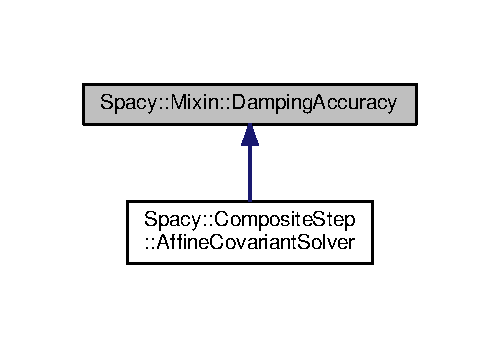
\includegraphics[width=240pt]{classSpacy_1_1Mixin_1_1DampingAccuracy__inherit__graph}
\end{center}
\end{figure}
\subsection*{Public Member Functions}
\begin{DoxyCompactItemize}
\item 
\hypertarget{classSpacy_1_1Mixin_1_1DampingAccuracy_a3cc2f537debc13218852ae8bfbcc4b37}{}{\bfseries Damping\+Accuracy} (double accuracy=1e-\/3) noexcept\label{classSpacy_1_1Mixin_1_1DampingAccuracy_a3cc2f537debc13218852ae8bfbcc4b37}

\item 
\hypertarget{classSpacy_1_1Mixin_1_1DampingAccuracy_af934aaf17595b7029d9a8ecec2561599}{}void {\bfseries set\+Damping\+Accuracy} (double accuracy) noexcept\label{classSpacy_1_1Mixin_1_1DampingAccuracy_af934aaf17595b7029d9a8ecec2561599}

\item 
\hypertarget{classSpacy_1_1Mixin_1_1DampingAccuracy_a070c4c1b64c4392c6b21478bcf4c4a75}{}double {\bfseries damping\+Accuracy} () const noexcept\label{classSpacy_1_1Mixin_1_1DampingAccuracy_a070c4c1b64c4392c6b21478bcf4c4a75}

\end{DoxyCompactItemize}


\subsection{Detailed Description}
Mixin class for the accuracy of damping factors. 

The documentation for this class was generated from the following file\+:\begin{DoxyCompactItemize}
\item 
Spacy/\+Util/\+Mixins/damping\+Accuracy.\+hh\end{DoxyCompactItemize}

\hypertarget{classSpacy_1_1DampingFactor}{}\section{Spacy\+:\+:Damping\+Factor Class Reference}
\label{classSpacy_1_1DampingFactor}\index{Spacy\+::\+Damping\+Factor@{Spacy\+::\+Damping\+Factor}}


A simple model of a damping factor $\nu$ that is computed up to a prescribed accuracy $\varepsilon$.  




{\ttfamily \#include $<$damping\+Factor.\+hh$>$}



Inheritance diagram for Spacy\+:\+:Damping\+Factor\+:\nopagebreak
\begin{figure}[H]
\begin{center}
\leavevmode
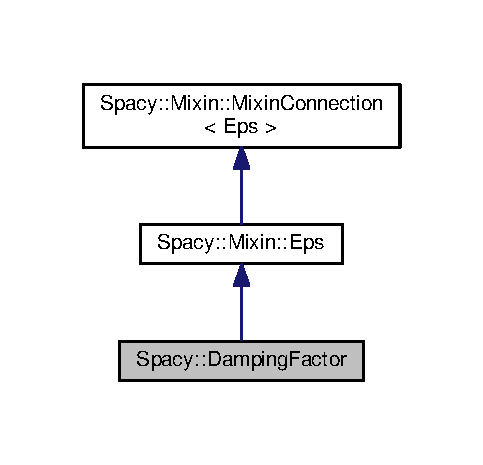
\includegraphics[width=232pt]{classSpacy_1_1DampingFactor__inherit__graph}
\end{center}
\end{figure}


Collaboration diagram for Spacy\+:\+:Damping\+Factor\+:\nopagebreak
\begin{figure}[H]
\begin{center}
\leavevmode
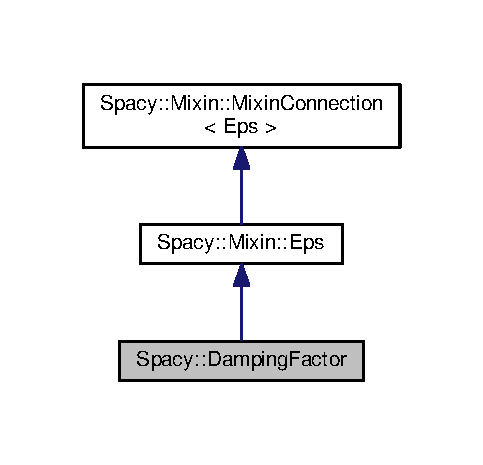
\includegraphics[width=232pt]{classSpacy_1_1DampingFactor__coll__graph}
\end{center}
\end{figure}
\subsection*{Public Member Functions}
\begin{DoxyCompactItemize}
\item 
\hyperlink{classSpacy_1_1DampingFactor_a03128fa4d2d17bd2024eaaff5a6cf03a}{Damping\+Factor} (\hyperlink{classSpacy_1_1Real}{Real} nu, double \hyperlink{classSpacy_1_1Mixin_1_1Eps_a40e2ba8f3abd2b5370ef41238cfaaf8b}{eps}=1e-\/3)
\begin{DoxyCompactList}\small\item\em Constructor. \end{DoxyCompactList}\item 
\hyperlink{classSpacy_1_1DampingFactor_a9e94f7d54ef502b804da36bde0ced9fe}{Damping\+Factor} (double nu, double \hyperlink{classSpacy_1_1Mixin_1_1Eps_a40e2ba8f3abd2b5370ef41238cfaaf8b}{eps}=1e-\/3)
\begin{DoxyCompactList}\small\item\em Constructor. \end{DoxyCompactList}\item 
\hyperlink{classSpacy_1_1DampingFactor}{Damping\+Factor} \& \hyperlink{classSpacy_1_1DampingFactor_a214beda25cc00fbe6c953308ba1ca9b3}{operator=} (\hyperlink{classSpacy_1_1Real}{Real} nu)
\begin{DoxyCompactList}\small\item\em Set damping factor $\nu$. \end{DoxyCompactList}\item 
\hyperlink{classSpacy_1_1DampingFactor}{Damping\+Factor} \& \hyperlink{classSpacy_1_1DampingFactor_a6790524473c91d6534ff93597fae3685}{operator=} (double nu)
\begin{DoxyCompactList}\small\item\em Set damping factor $\nu$. \end{DoxyCompactList}\item 
\hypertarget{classSpacy_1_1DampingFactor_ab2f626689cc8907bd9da2635e0bbd572}{}\hyperlink{classSpacy_1_1DampingFactor_ab2f626689cc8907bd9da2635e0bbd572}{operator Real} () const \label{classSpacy_1_1DampingFactor_ab2f626689cc8907bd9da2635e0bbd572}

\begin{DoxyCompactList}\small\item\em Access damping factor $\nu$. \end{DoxyCompactList}\item 
\hypertarget{classSpacy_1_1DampingFactor_aa14911dc85380f66fdb3541935cf893c}{}\hyperlink{classSpacy_1_1Real}{Real} \hyperlink{classSpacy_1_1DampingFactor_aa14911dc85380f66fdb3541935cf893c}{operator()} () const \label{classSpacy_1_1DampingFactor_aa14911dc85380f66fdb3541935cf893c}

\begin{DoxyCompactList}\small\item\em Access damping factor $\nu$. \end{DoxyCompactList}\item 
\hypertarget{classSpacy_1_1Mixin_1_1Eps_a1bbfd62541610d5d80f2782ab77158e4}{}void {\bfseries set\+Eps} (double \hyperlink{classSpacy_1_1Mixin_1_1Eps_a40e2ba8f3abd2b5370ef41238cfaaf8b}{eps})\label{classSpacy_1_1Mixin_1_1Eps_a1bbfd62541610d5d80f2782ab77158e4}

\item 
\hypertarget{classSpacy_1_1Mixin_1_1Eps_a40e2ba8f3abd2b5370ef41238cfaaf8b}{}double \hyperlink{classSpacy_1_1Mixin_1_1Eps_a40e2ba8f3abd2b5370ef41238cfaaf8b}{eps} () const noexcept\label{classSpacy_1_1Mixin_1_1Eps_a40e2ba8f3abd2b5370ef41238cfaaf8b}

\begin{DoxyCompactList}\small\item\em Access $\varepsilon$. \end{DoxyCompactList}\item 
\hypertarget{classSpacy_1_1Mixin_1_1Eps_a29e8c25dc3f1fdede57b8eb06f520fe1}{}double \hyperlink{classSpacy_1_1Mixin_1_1Eps_a29e8c25dc3f1fdede57b8eb06f520fe1}{sqrt\+Eps} () const noexcept\label{classSpacy_1_1Mixin_1_1Eps_a29e8c25dc3f1fdede57b8eb06f520fe1}

\begin{DoxyCompactList}\small\item\em Access $\sqrt\varepsilon$. \end{DoxyCompactList}\item 
\hypertarget{classSpacy_1_1Mixin_1_1Eps_a1879ebbf1b467cb4be36bcc63307018d}{}double \hyperlink{classSpacy_1_1Mixin_1_1Eps_a1879ebbf1b467cb4be36bcc63307018d}{cbrt\+Eps} () const noexcept\label{classSpacy_1_1Mixin_1_1Eps_a1879ebbf1b467cb4be36bcc63307018d}

\begin{DoxyCompactList}\small\item\em Access $\varepsilon^{1/3}$. \end{DoxyCompactList}\item 
\hypertarget{classSpacy_1_1Mixin_1_1Eps_a151216968daef3da5f5cdc0b957ce01b}{}void \hyperlink{classSpacy_1_1Mixin_1_1Eps_a151216968daef3da5f5cdc0b957ce01b}{update} (\hyperlink{classSpacy_1_1Mixin_1_1Eps_a51dbe0b9cc950e0f3dfd34a481f08ae4}{Eps} $\ast$changed\+Subject)\label{classSpacy_1_1Mixin_1_1Eps_a151216968daef3da5f5cdc0b957ce01b}

\begin{DoxyCompactList}\small\item\em update function for observer pattern. \end{DoxyCompactList}\item 
\hypertarget{classSpacy_1_1Mixin_1_1MixinConnection_abb5520ee6b22dd993d78f142939a1ed4}{}void \hyperlink{classSpacy_1_1Mixin_1_1MixinConnection_abb5520ee6b22dd993d78f142939a1ed4}{attach} (\hyperlink{classSpacy_1_1Mixin_1_1Eps_a51dbe0b9cc950e0f3dfd34a481f08ae4}{Eps} \&observer)\label{classSpacy_1_1Mixin_1_1MixinConnection_abb5520ee6b22dd993d78f142939a1ed4}

\begin{DoxyCompactList}\small\item\em Attach observer. \end{DoxyCompactList}\item 
\hypertarget{classSpacy_1_1Mixin_1_1MixinConnection_adda739590c487679c26f60e50aedb73f}{}void \hyperlink{classSpacy_1_1Mixin_1_1MixinConnection_adda739590c487679c26f60e50aedb73f}{detach} (\hyperlink{classSpacy_1_1Mixin_1_1Eps_a51dbe0b9cc950e0f3dfd34a481f08ae4}{Eps} \&observer)\label{classSpacy_1_1Mixin_1_1MixinConnection_adda739590c487679c26f60e50aedb73f}

\begin{DoxyCompactList}\small\item\em Detach observer. \end{DoxyCompactList}\item 
\hypertarget{classSpacy_1_1Mixin_1_1MixinConnection_a1ddeaa78a3bb4a38c2cca36d1f99fe36}{}void \hyperlink{classSpacy_1_1Mixin_1_1MixinConnection_a1ddeaa78a3bb4a38c2cca36d1f99fe36}{notify} ()\label{classSpacy_1_1Mixin_1_1MixinConnection_a1ddeaa78a3bb4a38c2cca36d1f99fe36}

\begin{DoxyCompactList}\small\item\em Notify observers about changes. \end{DoxyCompactList}\end{DoxyCompactItemize}


\subsection{Detailed Description}
A simple model of a damping factor $\nu$ that is computed up to a prescribed accuracy $\varepsilon$. 

\subsection{Constructor \& Destructor Documentation}
\hypertarget{classSpacy_1_1DampingFactor_a03128fa4d2d17bd2024eaaff5a6cf03a}{}\index{Spacy\+::\+Damping\+Factor@{Spacy\+::\+Damping\+Factor}!Damping\+Factor@{Damping\+Factor}}
\index{Damping\+Factor@{Damping\+Factor}!Spacy\+::\+Damping\+Factor@{Spacy\+::\+Damping\+Factor}}
\subsubsection[{Damping\+Factor}]{\setlength{\rightskip}{0pt plus 5cm}Spacy\+::\+Damping\+Factor\+::\+Damping\+Factor (
\begin{DoxyParamCaption}
\item[{{\bf Real}}]{nu, }
\item[{double}]{eps = {\ttfamily 1e-\/3}}
\end{DoxyParamCaption}
)}\label{classSpacy_1_1DampingFactor_a03128fa4d2d17bd2024eaaff5a6cf03a}


Constructor. 


\begin{DoxyParams}{Parameters}
{\em nu} & damping factor $\nu$ \\
\hline
{\em eps} & accuracy $\varepsilon$. \\
\hline
\end{DoxyParams}
\hypertarget{classSpacy_1_1DampingFactor_a9e94f7d54ef502b804da36bde0ced9fe}{}\index{Spacy\+::\+Damping\+Factor@{Spacy\+::\+Damping\+Factor}!Damping\+Factor@{Damping\+Factor}}
\index{Damping\+Factor@{Damping\+Factor}!Spacy\+::\+Damping\+Factor@{Spacy\+::\+Damping\+Factor}}
\subsubsection[{Damping\+Factor}]{\setlength{\rightskip}{0pt plus 5cm}Spacy\+::\+Damping\+Factor\+::\+Damping\+Factor (
\begin{DoxyParamCaption}
\item[{double}]{nu, }
\item[{double}]{eps = {\ttfamily 1e-\/3}}
\end{DoxyParamCaption}
)}\label{classSpacy_1_1DampingFactor_a9e94f7d54ef502b804da36bde0ced9fe}


Constructor. 


\begin{DoxyParams}{Parameters}
{\em nu} & damping factor $\nu$ \\
\hline
{\em eps} & accuracy $\varepsilon$. \\
\hline
\end{DoxyParams}


\subsection{Member Function Documentation}
\hypertarget{classSpacy_1_1DampingFactor_a214beda25cc00fbe6c953308ba1ca9b3}{}\index{Spacy\+::\+Damping\+Factor@{Spacy\+::\+Damping\+Factor}!operator=@{operator=}}
\index{operator=@{operator=}!Spacy\+::\+Damping\+Factor@{Spacy\+::\+Damping\+Factor}}
\subsubsection[{operator=}]{\setlength{\rightskip}{0pt plus 5cm}{\bf Damping\+Factor}\& Spacy\+::\+Damping\+Factor\+::operator= (
\begin{DoxyParamCaption}
\item[{{\bf Real}}]{nu}
\end{DoxyParamCaption}
)}\label{classSpacy_1_1DampingFactor_a214beda25cc00fbe6c953308ba1ca9b3}


Set damping factor $\nu$. 

If $ |\nu-1| < \varepsilon $ then $\nu$ is set to 1.


\begin{DoxyParams}{Parameters}
{\em nu} & damping factor \\
\hline
\end{DoxyParams}
\hypertarget{classSpacy_1_1DampingFactor_a6790524473c91d6534ff93597fae3685}{}\index{Spacy\+::\+Damping\+Factor@{Spacy\+::\+Damping\+Factor}!operator=@{operator=}}
\index{operator=@{operator=}!Spacy\+::\+Damping\+Factor@{Spacy\+::\+Damping\+Factor}}
\subsubsection[{operator=}]{\setlength{\rightskip}{0pt plus 5cm}{\bf Damping\+Factor}\& Spacy\+::\+Damping\+Factor\+::operator= (
\begin{DoxyParamCaption}
\item[{double}]{nu}
\end{DoxyParamCaption}
)}\label{classSpacy_1_1DampingFactor_a6790524473c91d6534ff93597fae3685}


Set damping factor $\nu$. 

If $ |\nu-1| < \varepsilon $ then $\nu$ is set to 1.


\begin{DoxyParams}{Parameters}
{\em nu} & damping factor \\
\hline
\end{DoxyParams}


The documentation for this class was generated from the following file\+:\begin{DoxyCompactItemize}
\item 
Spacy/\+Algorithm/damping\+Factor.\+hh\end{DoxyCompactItemize}

\hypertarget{classSpacy_1_1Mixin_1_1DecreaseCondition}{}\section{Spacy\+:\+:Mixin\+:\+:Decrease\+Condition Class Reference}
\label{classSpacy_1_1Mixin_1_1DecreaseCondition}\index{Spacy\+::\+Mixin\+::\+Decrease\+Condition@{Spacy\+::\+Mixin\+::\+Decrease\+Condition}}


Mixin class for accepting local models $m$ of nonlinear optimization problems $\min f(x)$.  




{\ttfamily \#include $<$decrease\+Condition.\+hh$>$}



Inheritance diagram for Spacy\+:\+:Mixin\+:\+:Decrease\+Condition\+:\nopagebreak
\begin{figure}[H]
\begin{center}
\leavevmode
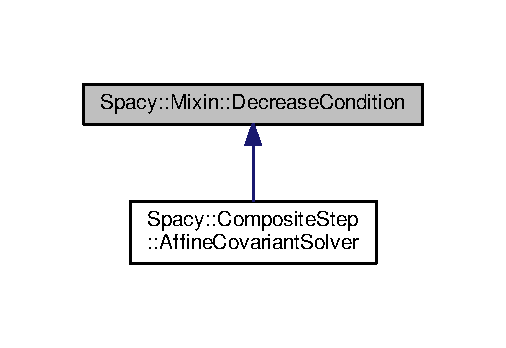
\includegraphics[width=243pt]{classSpacy_1_1Mixin_1_1DecreaseCondition__inherit__graph}
\end{center}
\end{figure}
\subsection*{Public Member Functions}
\begin{DoxyCompactItemize}
\item 
\hyperlink{classSpacy_1_1Mixin_1_1DecreaseCondition_abc3d63e53f4f7a81110a3b261e12c071}{Decrease\+Condition} (\hyperlink{classSpacy_1_1Real}{Real} \hyperlink{classSpacy_1_1Mixin_1_1DecreaseCondition_aeeda8b1d9f177fe5dd532e42de09ab44}{minimal\+Decrease}=0.\+5, \hyperlink{classSpacy_1_1Real}{Real} relaxed\+Minimal\+Decrease=0.\+1) noexcept
\begin{DoxyCompactList}\small\item\em Constructor. \end{DoxyCompactList}\item 
void \hyperlink{classSpacy_1_1Mixin_1_1DecreaseCondition_aabc5e2473edace0c87da7fbd9fa0ae61}{set\+Minimal\+Decrease} (\hyperlink{classSpacy_1_1Real}{Real} decrease) noexcept
\begin{DoxyCompactList}\small\item\em Set required minimal decrease. \end{DoxyCompactList}\item 
\hyperlink{classSpacy_1_1Real}{Real} \hyperlink{classSpacy_1_1Mixin_1_1DecreaseCondition_aeeda8b1d9f177fe5dd532e42de09ab44}{minimal\+Decrease} () const noexcept
\begin{DoxyCompactList}\small\item\em Access minimal decrease. \end{DoxyCompactList}\item 
void \hyperlink{classSpacy_1_1Mixin_1_1DecreaseCondition_a86d6a8c8fc683c31572fd818a102a362}{set\+Relaxed\+Minimal\+Decrease} (\hyperlink{classSpacy_1_1Real}{Real} decrease) noexcept
\begin{DoxyCompactList}\small\item\em Set relaxed minimal decrease. \end{DoxyCompactList}\item 
bool \hyperlink{classSpacy_1_1Mixin_1_1DecreaseCondition_a69c0c90daf14fc40461876f71c49ffc2}{acceptable\+Decrease} (\hyperlink{classSpacy_1_1Real}{Real} decrease) const noexcept
\begin{DoxyCompactList}\small\item\em Decide if measure relative decrease is acceptable. \end{DoxyCompactList}\item 
bool \hyperlink{classSpacy_1_1Mixin_1_1DecreaseCondition_a5ffb5bc008544db96d935a0ca34dcd24}{acceptable\+Relaxed\+Decrease} (\hyperlink{classSpacy_1_1Real}{Real} decrease) const noexcept
\begin{DoxyCompactList}\small\item\em Decide if measure relative decrease is acceptable with respect to the relaxed decrease condition. \end{DoxyCompactList}\end{DoxyCompactItemize}


\subsection{Detailed Description}
Mixin class for accepting local models $m$ of nonlinear optimization problems $\min f(x)$. 

\subsection{Constructor \& Destructor Documentation}
\hypertarget{classSpacy_1_1Mixin_1_1DecreaseCondition_abc3d63e53f4f7a81110a3b261e12c071}{}\index{Spacy\+::\+Mixin\+::\+Decrease\+Condition@{Spacy\+::\+Mixin\+::\+Decrease\+Condition}!Decrease\+Condition@{Decrease\+Condition}}
\index{Decrease\+Condition@{Decrease\+Condition}!Spacy\+::\+Mixin\+::\+Decrease\+Condition@{Spacy\+::\+Mixin\+::\+Decrease\+Condition}}
\subsubsection[{Decrease\+Condition}]{\setlength{\rightskip}{0pt plus 5cm}Spacy\+::\+Mixin\+::\+Decrease\+Condition\+::\+Decrease\+Condition (
\begin{DoxyParamCaption}
\item[{{\bf Real}}]{minimal\+Decrease = {\ttfamily 0.5}, }
\item[{{\bf Real}}]{relaxed\+Minimal\+Decrease = {\ttfamily 0.1}}
\end{DoxyParamCaption}
)\hspace{0.3cm}{\ttfamily [explicit]}, {\ttfamily [noexcept]}}\label{classSpacy_1_1Mixin_1_1DecreaseCondition_abc3d63e53f4f7a81110a3b261e12c071}


Constructor. 


\begin{DoxyParams}{Parameters}
{\em minimal\+Decrease} & minimal required decrease \\
\hline
{\em relaxed\+Minimal\+Decrease} & relaxed required decrease \\
\hline
\end{DoxyParams}


\subsection{Member Function Documentation}
\hypertarget{classSpacy_1_1Mixin_1_1DecreaseCondition_aabc5e2473edace0c87da7fbd9fa0ae61}{}\index{Spacy\+::\+Mixin\+::\+Decrease\+Condition@{Spacy\+::\+Mixin\+::\+Decrease\+Condition}!set\+Minimal\+Decrease@{set\+Minimal\+Decrease}}
\index{set\+Minimal\+Decrease@{set\+Minimal\+Decrease}!Spacy\+::\+Mixin\+::\+Decrease\+Condition@{Spacy\+::\+Mixin\+::\+Decrease\+Condition}}
\subsubsection[{set\+Minimal\+Decrease}]{\setlength{\rightskip}{0pt plus 5cm}void Spacy\+::\+Mixin\+::\+Decrease\+Condition\+::set\+Minimal\+Decrease (
\begin{DoxyParamCaption}
\item[{{\bf Real}}]{decrease}
\end{DoxyParamCaption}
)\hspace{0.3cm}{\ttfamily [noexcept]}}\label{classSpacy_1_1Mixin_1_1DecreaseCondition_aabc5e2473edace0c87da7fbd9fa0ae61}


Set required minimal decrease. 


\begin{DoxyParams}{Parameters}
{\em decrease} & minimal required decrease \\
\hline
\end{DoxyParams}
\hypertarget{classSpacy_1_1Mixin_1_1DecreaseCondition_aeeda8b1d9f177fe5dd532e42de09ab44}{}\index{Spacy\+::\+Mixin\+::\+Decrease\+Condition@{Spacy\+::\+Mixin\+::\+Decrease\+Condition}!minimal\+Decrease@{minimal\+Decrease}}
\index{minimal\+Decrease@{minimal\+Decrease}!Spacy\+::\+Mixin\+::\+Decrease\+Condition@{Spacy\+::\+Mixin\+::\+Decrease\+Condition}}
\subsubsection[{minimal\+Decrease}]{\setlength{\rightskip}{0pt plus 5cm}{\bf Real} Spacy\+::\+Mixin\+::\+Decrease\+Condition\+::minimal\+Decrease (
\begin{DoxyParamCaption}
{}
\end{DoxyParamCaption}
) const\hspace{0.3cm}{\ttfamily [noexcept]}}\label{classSpacy_1_1Mixin_1_1DecreaseCondition_aeeda8b1d9f177fe5dd532e42de09ab44}


Access minimal decrease. 

\begin{DoxyReturn}{Returns}
minimal decrease 
\end{DoxyReturn}
\hypertarget{classSpacy_1_1Mixin_1_1DecreaseCondition_a86d6a8c8fc683c31572fd818a102a362}{}\index{Spacy\+::\+Mixin\+::\+Decrease\+Condition@{Spacy\+::\+Mixin\+::\+Decrease\+Condition}!set\+Relaxed\+Minimal\+Decrease@{set\+Relaxed\+Minimal\+Decrease}}
\index{set\+Relaxed\+Minimal\+Decrease@{set\+Relaxed\+Minimal\+Decrease}!Spacy\+::\+Mixin\+::\+Decrease\+Condition@{Spacy\+::\+Mixin\+::\+Decrease\+Condition}}
\subsubsection[{set\+Relaxed\+Minimal\+Decrease}]{\setlength{\rightskip}{0pt plus 5cm}void Spacy\+::\+Mixin\+::\+Decrease\+Condition\+::set\+Relaxed\+Minimal\+Decrease (
\begin{DoxyParamCaption}
\item[{{\bf Real}}]{decrease}
\end{DoxyParamCaption}
)\hspace{0.3cm}{\ttfamily [noexcept]}}\label{classSpacy_1_1Mixin_1_1DecreaseCondition_a86d6a8c8fc683c31572fd818a102a362}


Set relaxed minimal decrease. 


\begin{DoxyParams}{Parameters}
{\em decrease} & relaxed required decrease\\
\hline
\end{DoxyParams}
This is used for deciding about rejecting tangential steps in Composite\+Steps\+::\+Affine\+Covariant\+Solver. \hypertarget{classSpacy_1_1Mixin_1_1DecreaseCondition_a69c0c90daf14fc40461876f71c49ffc2}{}\index{Spacy\+::\+Mixin\+::\+Decrease\+Condition@{Spacy\+::\+Mixin\+::\+Decrease\+Condition}!acceptable\+Decrease@{acceptable\+Decrease}}
\index{acceptable\+Decrease@{acceptable\+Decrease}!Spacy\+::\+Mixin\+::\+Decrease\+Condition@{Spacy\+::\+Mixin\+::\+Decrease\+Condition}}
\subsubsection[{acceptable\+Decrease}]{\setlength{\rightskip}{0pt plus 5cm}bool Spacy\+::\+Mixin\+::\+Decrease\+Condition\+::acceptable\+Decrease (
\begin{DoxyParamCaption}
\item[{{\bf Real}}]{decrease}
\end{DoxyParamCaption}
) const\hspace{0.3cm}{\ttfamily [noexcept]}}\label{classSpacy_1_1Mixin_1_1DecreaseCondition_a69c0c90daf14fc40461876f71c49ffc2}


Decide if measure relative decrease is acceptable. 


\begin{DoxyParams}{Parameters}
{\em decrease} & measured relative decrease $\delta m/\delta f$. \\
\hline
\end{DoxyParams}
\hypertarget{classSpacy_1_1Mixin_1_1DecreaseCondition_a5ffb5bc008544db96d935a0ca34dcd24}{}\index{Spacy\+::\+Mixin\+::\+Decrease\+Condition@{Spacy\+::\+Mixin\+::\+Decrease\+Condition}!acceptable\+Relaxed\+Decrease@{acceptable\+Relaxed\+Decrease}}
\index{acceptable\+Relaxed\+Decrease@{acceptable\+Relaxed\+Decrease}!Spacy\+::\+Mixin\+::\+Decrease\+Condition@{Spacy\+::\+Mixin\+::\+Decrease\+Condition}}
\subsubsection[{acceptable\+Relaxed\+Decrease}]{\setlength{\rightskip}{0pt plus 5cm}bool Spacy\+::\+Mixin\+::\+Decrease\+Condition\+::acceptable\+Relaxed\+Decrease (
\begin{DoxyParamCaption}
\item[{{\bf Real}}]{decrease}
\end{DoxyParamCaption}
) const\hspace{0.3cm}{\ttfamily [noexcept]}}\label{classSpacy_1_1Mixin_1_1DecreaseCondition_a5ffb5bc008544db96d935a0ca34dcd24}


Decide if measure relative decrease is acceptable with respect to the relaxed decrease condition. 


\begin{DoxyParams}{Parameters}
{\em decrease} & measured relative decrease $\delta m/\delta f$. \\
\hline
\end{DoxyParams}


The documentation for this class was generated from the following file\+:\begin{DoxyCompactItemize}
\item 
Spacy/\+Util/\+Mixins/decrease\+Condition.\+hh\end{DoxyCompactItemize}

\hypertarget{classSpacy_1_1Kaskade_1_1DirectSolver}{}\section{Spacy\+:\+:Kaskade\+:\+:Direct\+Solver$<$ Kaskade\+Operator, Ansatz\+Variable\+Description, Test\+Variable\+Description $>$ Class Template Reference}
\label{classSpacy_1_1Kaskade_1_1DirectSolver}\index{Spacy\+::\+Kaskade\+::\+Direct\+Solver$<$ Kaskade\+Operator, Ansatz\+Variable\+Description, Test\+Variable\+Description $>$@{Spacy\+::\+Kaskade\+::\+Direct\+Solver$<$ Kaskade\+Operator, Ansatz\+Variable\+Description, Test\+Variable\+Description $>$}}


Direct solver interface for Kaskade 7.  




{\ttfamily \#include $<$direct\+Solver.\+hh$>$}



Inheritance diagram for Spacy\+:\+:Kaskade\+:\+:Direct\+Solver$<$ Kaskade\+Operator, Ansatz\+Variable\+Description, Test\+Variable\+Description $>$\+:\nopagebreak
\begin{figure}[H]
\begin{center}
\leavevmode
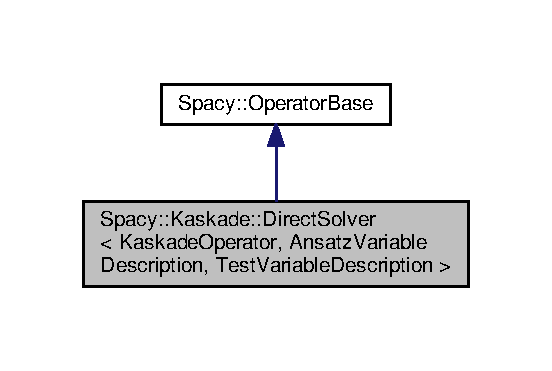
\includegraphics[width=265pt]{classSpacy_1_1Kaskade_1_1DirectSolver__inherit__graph}
\end{center}
\end{figure}


Collaboration diagram for Spacy\+:\+:Kaskade\+:\+:Direct\+Solver$<$ Kaskade\+Operator, Ansatz\+Variable\+Description, Test\+Variable\+Description $>$\+:\nopagebreak
\begin{figure}[H]
\begin{center}
\leavevmode
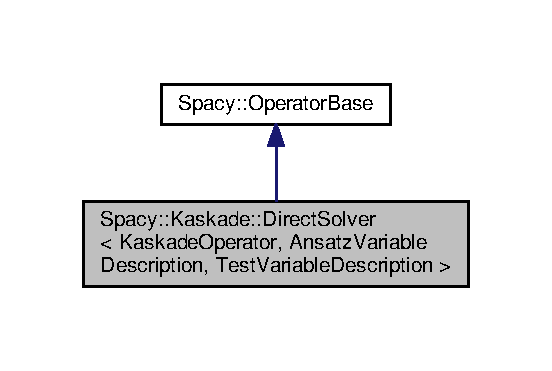
\includegraphics[width=265pt]{classSpacy_1_1Kaskade_1_1DirectSolver__coll__graph}
\end{center}
\end{figure}
\subsection*{Public Member Functions}
\begin{DoxyCompactItemize}
\item 
\hyperlink{classSpacy_1_1Kaskade_1_1DirectSolver_a52ed83fd0cd00bc57d4f09963dfe2e98_a52ed83fd0cd00bc57d4f09963dfe2e98}{Direct\+Solver} (Kaskade\+Operator A, const \hyperlink{classSpacy_1_1VectorSpace}{Vector\+Space} \&\hyperlink{classSpacy_1_1OperatorBase_a2588f9b3e0188820c4c494e63293dc6f_a2588f9b3e0188820c4c494e63293dc6f}{domain}, const \hyperlink{classSpacy_1_1VectorSpace}{Vector\+Space} \&\hyperlink{classSpacy_1_1OperatorBase_ab19d3b7a6f290b1079248f1e567e53d6_ab19d3b7a6f290b1079248f1e567e53d6}{range}, Direct\+Type direct\+Solver=Direct\+Type\+::\+M\+U\+M\+P\+S, Matrix\+Properties property=Matrix\+Properties\+::\+G\+E\+N\+E\+R\+A\+L)
\begin{DoxyCompactList}\small\item\em Constructor. \end{DoxyCompactList}\item 
\hypertarget{classSpacy_1_1Kaskade_1_1DirectSolver_ae3b85c906968d662c23bdde7df96ca87}{}\+::\hyperlink{classSpacy_1_1Vector}{Spacy\+::\+Vector} \hyperlink{classSpacy_1_1Kaskade_1_1DirectSolver_ae3b85c906968d662c23bdde7df96ca87}{operator()} (const \+::\hyperlink{classSpacy_1_1Vector}{Spacy\+::\+Vector} \&x) const \label{classSpacy_1_1Kaskade_1_1DirectSolver_ae3b85c906968d662c23bdde7df96ca87}

\begin{DoxyCompactList}\small\item\em Compute $A^{-1}x$. \end{DoxyCompactList}\item 
const \hyperlink{classSpacy_1_1VectorSpace}{Vector\+Space} \& \hyperlink{classSpacy_1_1OperatorBase_a2588f9b3e0188820c4c494e63293dc6f_a2588f9b3e0188820c4c494e63293dc6f}{domain} () const 
\begin{DoxyCompactList}\small\item\em Access domain space $X$. \end{DoxyCompactList}\item 
const \hyperlink{classSpacy_1_1VectorSpace}{Vector\+Space} \& \hyperlink{classSpacy_1_1OperatorBase_ab19d3b7a6f290b1079248f1e567e53d6_ab19d3b7a6f290b1079248f1e567e53d6}{range} () const 
\begin{DoxyCompactList}\small\item\em Access range space $Y$. \end{DoxyCompactList}\end{DoxyCompactItemize}


\subsection{Detailed Description}
\subsubsection*{template$<$class Kaskade\+Operator, class Ansatz\+Variable\+Description, class Test\+Variable\+Description$>$class Spacy\+::\+Kaskade\+::\+Direct\+Solver$<$ Kaskade\+Operator, Ansatz\+Variable\+Description, Test\+Variable\+Description $>$}

Direct solver interface for Kaskade 7. 

Performs lazy construction of the solver. 

\subsection{Constructor \& Destructor Documentation}
\hypertarget{classSpacy_1_1Kaskade_1_1DirectSolver_a52ed83fd0cd00bc57d4f09963dfe2e98_a52ed83fd0cd00bc57d4f09963dfe2e98}{}\index{Spacy\+::\+Kaskade\+::\+Direct\+Solver@{Spacy\+::\+Kaskade\+::\+Direct\+Solver}!Direct\+Solver@{Direct\+Solver}}
\index{Direct\+Solver@{Direct\+Solver}!Spacy\+::\+Kaskade\+::\+Direct\+Solver@{Spacy\+::\+Kaskade\+::\+Direct\+Solver}}
\subsubsection[{Direct\+Solver}]{\setlength{\rightskip}{0pt plus 5cm}template$<$class Kaskade\+Operator , class Ansatz\+Variable\+Description , class Test\+Variable\+Description $>$ {\bf Spacy\+::\+Kaskade\+::\+Direct\+Solver}$<$ Kaskade\+Operator, Ansatz\+Variable\+Description, Test\+Variable\+Description $>$\+::{\bf Direct\+Solver} (
\begin{DoxyParamCaption}
\item[{Kaskade\+Operator}]{A, }
\item[{const {\bf Vector\+Space} \&}]{domain, }
\item[{const {\bf Vector\+Space} \&}]{range, }
\item[{Direct\+Type}]{direct\+Solver = {\ttfamily DirectType\+:\+:MUMPS}, }
\item[{Matrix\+Properties}]{property = {\ttfamily MatrixProperties\+:\+:GENERAL}}
\end{DoxyParamCaption}
)\hspace{0.3cm}{\ttfamily [inline]}}\label{classSpacy_1_1Kaskade_1_1DirectSolver_a52ed83fd0cd00bc57d4f09963dfe2e98_a52ed83fd0cd00bc57d4f09963dfe2e98}


Constructor. 


\begin{DoxyParams}{Parameters}
{\em A} & Kaskade operator (i.\+e., Assembled\+Galerkin\+Operator or Matrix\+Represented\+Operator) \\
\hline
{\em spaces} & boost fusion forward sequence of space pointers required to initialize temporary storage \\
\hline
{\em domain} & domain space of the solver \\
\hline
{\em range} & range space of the solver \\
\hline
{\em direct\+Solver} & solver type (Direct\+Type\+::\+M\+U\+M\+P\+S (default), Direct\+Type\+::\+U\+M\+F\+P\+A\+C\+K, Direct\+Type\+::\+U\+M\+F\+P\+A\+C\+K3264 or Direct\+Type\+::\+S\+U\+P\+E\+R\+L\+U) \\
\hline
{\em property} & matrix property (Matrix\+Properties\+::\+G\+E\+N\+E\+R\+A\+L (default) or Matrix\+Properties\+::\+S\+Y\+M\+M\+E\+T\+R\+I\+C) \\
\hline
\end{DoxyParams}


\subsection{Member Function Documentation}
\hypertarget{classSpacy_1_1OperatorBase_a2588f9b3e0188820c4c494e63293dc6f_a2588f9b3e0188820c4c494e63293dc6f}{}\index{Spacy\+::\+Kaskade\+::\+Direct\+Solver@{Spacy\+::\+Kaskade\+::\+Direct\+Solver}!domain@{domain}}
\index{domain@{domain}!Spacy\+::\+Kaskade\+::\+Direct\+Solver@{Spacy\+::\+Kaskade\+::\+Direct\+Solver}}
\subsubsection[{domain}]{\setlength{\rightskip}{0pt plus 5cm}const {\bf Vector\+Space}\& Spacy\+::\+Operator\+Base\+::domain (
\begin{DoxyParamCaption}
{}
\end{DoxyParamCaption}
) const\hspace{0.3cm}{\ttfamily [inherited]}}\label{classSpacy_1_1OperatorBase_a2588f9b3e0188820c4c494e63293dc6f_a2588f9b3e0188820c4c494e63293dc6f}


Access domain space $X$. 

\begin{DoxyReturn}{Returns}
domain space $X$. 
\end{DoxyReturn}
\hypertarget{classSpacy_1_1OperatorBase_ab19d3b7a6f290b1079248f1e567e53d6_ab19d3b7a6f290b1079248f1e567e53d6}{}\index{Spacy\+::\+Kaskade\+::\+Direct\+Solver@{Spacy\+::\+Kaskade\+::\+Direct\+Solver}!range@{range}}
\index{range@{range}!Spacy\+::\+Kaskade\+::\+Direct\+Solver@{Spacy\+::\+Kaskade\+::\+Direct\+Solver}}
\subsubsection[{range}]{\setlength{\rightskip}{0pt plus 5cm}const {\bf Vector\+Space}\& Spacy\+::\+Operator\+Base\+::range (
\begin{DoxyParamCaption}
{}
\end{DoxyParamCaption}
) const\hspace{0.3cm}{\ttfamily [inherited]}}\label{classSpacy_1_1OperatorBase_ab19d3b7a6f290b1079248f1e567e53d6_ab19d3b7a6f290b1079248f1e567e53d6}


Access range space $Y$. 

\begin{DoxyReturn}{Returns}
range space $Y$. 
\end{DoxyReturn}


The documentation for this class was generated from the following file\+:\begin{DoxyCompactItemize}
\item 
Spacy/\+Adapter/\+Kaskade/direct\+Solver.\+hh\end{DoxyCompactItemize}

\hypertarget{classSpacy_1_1Kaskade_1_1DLY}{}\section{Spacy\+:\+:Kaskade\+:\+:D\+L\+Y$<$ Definition, Ansatz\+Vars, Ansatz\+Vars\+Extension $>$ Class Template Reference}
\label{classSpacy_1_1Kaskade_1_1DLY}\index{Spacy\+::\+Kaskade\+::\+D\+L\+Y$<$ Definition, Ansatz\+Vars, Ansatz\+Vars\+Extension $>$@{Spacy\+::\+Kaskade\+::\+D\+L\+Y$<$ Definition, Ansatz\+Vars, Ansatz\+Vars\+Extension $>$}}


Inheritance diagram for Spacy\+:\+:Kaskade\+:\+:D\+L\+Y$<$ Definition, Ansatz\+Vars, Ansatz\+Vars\+Extension $>$\+:\nopagebreak
\begin{figure}[H]
\begin{center}
\leavevmode
\includegraphics[width=237pt]{classSpacy_1_1Kaskade_1_1DLY__inherit__graph}
\end{center}
\end{figure}


Collaboration diagram for Spacy\+:\+:Kaskade\+:\+:D\+L\+Y$<$ Definition, Ansatz\+Vars, Ansatz\+Vars\+Extension $>$\+:\nopagebreak
\begin{figure}[H]
\begin{center}
\leavevmode
\includegraphics[width=237pt]{classSpacy_1_1Kaskade_1_1DLY__coll__graph}
\end{center}
\end{figure}
\subsection*{Public Member Functions}
\begin{DoxyCompactItemize}
\item 
\hypertarget{classSpacy_1_1Kaskade_1_1DLY_ad6ad6ff4ac8b00b0f6c3a607e99f0a81}{}{\footnotesize template$<$class... Args$>$ }\\{\bfseries D\+L\+Y} (\+::Kaskade\+::\+Grid\+Manager$<$ Grid $>$ \&grid\+Manager, const Ansatz\+Vars \&ansatz\+Vars, const Ansatz\+Vars\+Extension \&ansatz\+Vars\+Extension, const Args \&...args)\label{classSpacy_1_1Kaskade_1_1DLY_ad6ad6ff4ac8b00b0f6c3a607e99f0a81}

\item 
\hypertarget{classSpacy_1_1Kaskade_1_1DLY_ad65881ff822a7407900909dcb8fad771}{}bool {\bfseries operator()} (const \+::\hyperlink{classSpacy_1_1Vector}{Spacy\+::\+Vector} \&x, const \+::\hyperlink{classSpacy_1_1Vector}{Spacy\+::\+Vector} \&dx)\label{classSpacy_1_1Kaskade_1_1DLY_ad65881ff822a7407900909dcb8fad771}

\item 
void \hyperlink{classSpacy_1_1Mixin_1_1RelativeAccuracy_aee88b71e80aca446a179f1310408a1e3_aee88b71e80aca446a179f1310408a1e3}{set\+Relative\+Accuracy} (double accuracy)
\begin{DoxyCompactList}\small\item\em Set relative accuracy. \end{DoxyCompactList}\item 
double \hyperlink{classSpacy_1_1Mixin_1_1RelativeAccuracy_a1da618cf9265c2edae354524df4a7f8a_a1da618cf9265c2edae354524df4a7f8a}{relative\+Accuracy} () const noexcept
\begin{DoxyCompactList}\small\item\em Access relative accuracy. \end{DoxyCompactList}\item 
void \hyperlink{classSpacy_1_1Mixin_1_1RelativeAccuracy_ae299bb5419df551cc93c6397e5b1b58b_ae299bb5419df551cc93c6397e5b1b58b}{attach\+Relative\+Accuracy} (\hyperlink{classSpacy_1_1Mixin_1_1RelativeAccuracy_ad843319a8782b47291fa31334e8bbd2a_ad843319a8782b47291fa31334e8bbd2a}{Relative\+Accuracy} \&other)
\begin{DoxyCompactList}\small\item\em Attach \hyperlink{classSpacy_1_1Mixin_1_1RelativeAccuracy}{Relative\+Accuracy}. \end{DoxyCompactList}\item 
\hypertarget{classSpacy_1_1Mixin_1_1RelativeAccuracy_a2636cde30aab8415e19e25fc12489e57}{}void \hyperlink{classSpacy_1_1Mixin_1_1RelativeAccuracy_a2636cde30aab8415e19e25fc12489e57}{detach\+Relative\+Accuracy} (\hyperlink{classSpacy_1_1Mixin_1_1RelativeAccuracy_ad843319a8782b47291fa31334e8bbd2a_ad843319a8782b47291fa31334e8bbd2a}{Relative\+Accuracy} \&other)\label{classSpacy_1_1Mixin_1_1RelativeAccuracy_a2636cde30aab8415e19e25fc12489e57}

\begin{DoxyCompactList}\small\item\em Detach \hyperlink{classSpacy_1_1Mixin_1_1RelativeAccuracy}{Relative\+Accuracy} before it gets deleted. \end{DoxyCompactList}\item 
\hypertarget{classSpacy_1_1Mixin_1_1RelativeAccuracy_acf0b58224d9a2879d05b5d2947f37527}{}void \hyperlink{classSpacy_1_1Mixin_1_1RelativeAccuracy_acf0b58224d9a2879d05b5d2947f37527}{update} (\hyperlink{classSpacy_1_1Mixin_1_1RelativeAccuracy_ad843319a8782b47291fa31334e8bbd2a_ad843319a8782b47291fa31334e8bbd2a}{Relative\+Accuracy} $\ast$changed\+Subject)\label{classSpacy_1_1Mixin_1_1RelativeAccuracy_acf0b58224d9a2879d05b5d2947f37527}

\begin{DoxyCompactList}\small\item\em update function for observer pattern. \end{DoxyCompactList}\end{DoxyCompactItemize}
\subsection*{Protected Member Functions}
\begin{DoxyCompactItemize}
\item 
\hypertarget{classSpacy_1_1Mixin_1_1MixinConnection_abb5520ee6b22dd993d78f142939a1ed4}{}void \hyperlink{classSpacy_1_1Mixin_1_1MixinConnection_abb5520ee6b22dd993d78f142939a1ed4}{attach} (\hyperlink{classSpacy_1_1Mixin_1_1RelativeAccuracy_ad843319a8782b47291fa31334e8bbd2a_ad843319a8782b47291fa31334e8bbd2a}{Relative\+Accuracy} \&observer)\label{classSpacy_1_1Mixin_1_1MixinConnection_abb5520ee6b22dd993d78f142939a1ed4}

\begin{DoxyCompactList}\small\item\em Attach observer. \end{DoxyCompactList}\item 
\hypertarget{classSpacy_1_1Mixin_1_1MixinConnection_adda739590c487679c26f60e50aedb73f}{}void \hyperlink{classSpacy_1_1Mixin_1_1MixinConnection_adda739590c487679c26f60e50aedb73f}{detach} (\hyperlink{classSpacy_1_1Mixin_1_1RelativeAccuracy_ad843319a8782b47291fa31334e8bbd2a_ad843319a8782b47291fa31334e8bbd2a}{Relative\+Accuracy} \&observer)\label{classSpacy_1_1Mixin_1_1MixinConnection_adda739590c487679c26f60e50aedb73f}

\begin{DoxyCompactList}\small\item\em Detach observer. \end{DoxyCompactList}\item 
\hypertarget{classSpacy_1_1Mixin_1_1MixinConnection_a1ddeaa78a3bb4a38c2cca36d1f99fe36}{}void \hyperlink{classSpacy_1_1Mixin_1_1MixinConnection_a1ddeaa78a3bb4a38c2cca36d1f99fe36}{notify} ()\label{classSpacy_1_1Mixin_1_1MixinConnection_a1ddeaa78a3bb4a38c2cca36d1f99fe36}

\begin{DoxyCompactList}\small\item\em Notify observers about changes. \end{DoxyCompactList}\end{DoxyCompactItemize}


\subsection{Member Function Documentation}
\hypertarget{classSpacy_1_1Mixin_1_1RelativeAccuracy_ae299bb5419df551cc93c6397e5b1b58b_ae299bb5419df551cc93c6397e5b1b58b}{}\index{Spacy\+::\+Kaskade\+::\+D\+L\+Y@{Spacy\+::\+Kaskade\+::\+D\+L\+Y}!attach\+Relative\+Accuracy@{attach\+Relative\+Accuracy}}
\index{attach\+Relative\+Accuracy@{attach\+Relative\+Accuracy}!Spacy\+::\+Kaskade\+::\+D\+L\+Y@{Spacy\+::\+Kaskade\+::\+D\+L\+Y}}
\subsubsection[{attach\+Relative\+Accuracy}]{\setlength{\rightskip}{0pt plus 5cm}void Spacy\+::\+Mixin\+::\+Relative\+Accuracy\+::attach\+Relative\+Accuracy (
\begin{DoxyParamCaption}
\item[{{\bf Relative\+Accuracy} \&}]{other}
\end{DoxyParamCaption}
)\hspace{0.3cm}{\ttfamily [inherited]}}\label{classSpacy_1_1Mixin_1_1RelativeAccuracy_ae299bb5419df551cc93c6397e5b1b58b_ae299bb5419df551cc93c6397e5b1b58b}


Attach \hyperlink{classSpacy_1_1Mixin_1_1RelativeAccuracy}{Relative\+Accuracy}. 

When \hyperlink{classSpacy_1_1Mixin_1_1RelativeAccuracy_aee88b71e80aca446a179f1310408a1e3_aee88b71e80aca446a179f1310408a1e3}{set\+Relative\+Accuracy(double relative\+Accuracy)} is called, then also other.\+set\+Relative\+Accuracy(relative\+Accuracy) is invoked. \hypertarget{classSpacy_1_1Mixin_1_1RelativeAccuracy_a1da618cf9265c2edae354524df4a7f8a_a1da618cf9265c2edae354524df4a7f8a}{}\index{Spacy\+::\+Kaskade\+::\+D\+L\+Y@{Spacy\+::\+Kaskade\+::\+D\+L\+Y}!relative\+Accuracy@{relative\+Accuracy}}
\index{relative\+Accuracy@{relative\+Accuracy}!Spacy\+::\+Kaskade\+::\+D\+L\+Y@{Spacy\+::\+Kaskade\+::\+D\+L\+Y}}
\subsubsection[{relative\+Accuracy}]{\setlength{\rightskip}{0pt plus 5cm}double Spacy\+::\+Mixin\+::\+Relative\+Accuracy\+::relative\+Accuracy (
\begin{DoxyParamCaption}
{}
\end{DoxyParamCaption}
) const\hspace{0.3cm}{\ttfamily [noexcept]}, {\ttfamily [inherited]}}\label{classSpacy_1_1Mixin_1_1RelativeAccuracy_a1da618cf9265c2edae354524df4a7f8a_a1da618cf9265c2edae354524df4a7f8a}


Access relative accuracy. 

\begin{DoxyReturn}{Returns}
relative accuracy 
\end{DoxyReturn}
\hypertarget{classSpacy_1_1Mixin_1_1RelativeAccuracy_aee88b71e80aca446a179f1310408a1e3_aee88b71e80aca446a179f1310408a1e3}{}\index{Spacy\+::\+Kaskade\+::\+D\+L\+Y@{Spacy\+::\+Kaskade\+::\+D\+L\+Y}!set\+Relative\+Accuracy@{set\+Relative\+Accuracy}}
\index{set\+Relative\+Accuracy@{set\+Relative\+Accuracy}!Spacy\+::\+Kaskade\+::\+D\+L\+Y@{Spacy\+::\+Kaskade\+::\+D\+L\+Y}}
\subsubsection[{set\+Relative\+Accuracy}]{\setlength{\rightskip}{0pt plus 5cm}void Spacy\+::\+Mixin\+::\+Relative\+Accuracy\+::set\+Relative\+Accuracy (
\begin{DoxyParamCaption}
\item[{double}]{accuracy}
\end{DoxyParamCaption}
)\hspace{0.3cm}{\ttfamily [inherited]}}\label{classSpacy_1_1Mixin_1_1RelativeAccuracy_aee88b71e80aca446a179f1310408a1e3_aee88b71e80aca446a179f1310408a1e3}


Set relative accuracy. 


\begin{DoxyParams}{Parameters}
{\em accuracy} & relative accuracy \\
\hline
\end{DoxyParams}


The documentation for this class was generated from the following file\+:\begin{DoxyCompactItemize}
\item 
Spacy/\+Adapter/\+Kaskade/dly.\+hh\end{DoxyCompactItemize}

\hypertarget{classSpacy_1_1Kaskade_1_1ErrorDistribution_1_1DomainCache}{}\section{Spacy\+:\+:Kaskade\+:\+:Error\+Distribution$<$ Functional, Extended\+Ansatz\+Vars $>$\+:\+:Domain\+Cache Class Reference}
\label{classSpacy_1_1Kaskade_1_1ErrorDistribution_1_1DomainCache}\index{Spacy\+::\+Kaskade\+::\+Error\+Distribution$<$ Functional, Extended\+Ansatz\+Vars $>$\+::\+Domain\+Cache@{Spacy\+::\+Kaskade\+::\+Error\+Distribution$<$ Functional, Extended\+Ansatz\+Vars $>$\+::\+Domain\+Cache}}
\subsection*{Public Member Functions}
\begin{DoxyCompactItemize}
\item 
\hypertarget{classSpacy_1_1Kaskade_1_1ErrorDistribution_1_1DomainCache_a4d795bf827e132c749bf187a898e0cae}{}{\bfseries Domain\+Cache} (\hyperlink{classSpacy_1_1Kaskade_1_1ErrorDistribution}{Error\+Distribution} const \&f\+\_\+, typename Origin\+Vars\+::\+Variable\+Set const \&, int flags=7)\label{classSpacy_1_1Kaskade_1_1ErrorDistribution_1_1DomainCache_a4d795bf827e132c749bf187a898e0cae}

\item 
\hypertarget{classSpacy_1_1Kaskade_1_1ErrorDistribution_1_1DomainCache_a92c3a6e34c52903f5beb0c74228e3564}{}{\footnotesize template$<$class Entity $>$ }\\void {\bfseries move\+To} (Entity const \&entity)\label{classSpacy_1_1Kaskade_1_1ErrorDistribution_1_1DomainCache_a92c3a6e34c52903f5beb0c74228e3564}

\item 
\hypertarget{classSpacy_1_1Kaskade_1_1ErrorDistribution_1_1DomainCache_ae554faae1e9ec499b26194ddd3bdc522}{}{\footnotesize template$<$class Position , class Evaluators $>$ }\\void {\bfseries evaluate\+At} (Position const \&x\+\_\+, Evaluators const \&evaluators)\label{classSpacy_1_1Kaskade_1_1ErrorDistribution_1_1DomainCache_ae554faae1e9ec499b26194ddd3bdc522}

\item 
\hypertarget{classSpacy_1_1Kaskade_1_1ErrorDistribution_1_1DomainCache_a69892afb6c248b274005e99f514388c8}{}Scalar {\bfseries d0} () const \label{classSpacy_1_1Kaskade_1_1ErrorDistribution_1_1DomainCache_a69892afb6c248b274005e99f514388c8}

\item 
\hypertarget{classSpacy_1_1Kaskade_1_1ErrorDistribution_1_1DomainCache_a392dcc0c91960b8c11ffe34e9ffd4a2b}{}{\footnotesize template$<$int row, int dim$>$ }\\\hyperlink{classDune_1_1FieldVector}{Dune\+::\+Field\+Vector}$<$ Scalar, Test\+Vars\+::template Components$<$ row $>$\+::m $>$ {\bfseries d1} (\+::Kaskade\+::\+Variational\+Arg$<$ Scalar, dim $>$ const \&arg) const \label{classSpacy_1_1Kaskade_1_1ErrorDistribution_1_1DomainCache_a392dcc0c91960b8c11ffe34e9ffd4a2b}

\item 
\hypertarget{classSpacy_1_1Kaskade_1_1ErrorDistribution_1_1DomainCache_af8c82b3c6c53e77556c1f208388a2074}{}{\footnotesize template$<$int row, int col, int dim$>$ }\\auto {\bfseries d2} (\+::Kaskade\+::\+Variational\+Arg$<$ Scalar, dim $>$ const \&,\+::Kaskade\+::\+Variational\+Arg$<$ Scalar, dim $>$ const \&) const \label{classSpacy_1_1Kaskade_1_1ErrorDistribution_1_1DomainCache_af8c82b3c6c53e77556c1f208388a2074}

\end{DoxyCompactItemize}


The documentation for this class was generated from the following file\+:\begin{DoxyCompactItemize}
\item 
Spacy/\+Adapter/\+Kaskade/\+Definitions/error\+\_\+distribution.\+hh\end{DoxyCompactItemize}

\hypertarget{classSpacy_1_1FEniCS_1_1DynamicC1Operator}{}\section{Spacy\+:\+:F\+Eni\+C\+S\+:\+:Dynamic\+C1\+Operator$<$ Residual\+Form, Jacobian\+Form, Mass\+Form, Source $>$ Class Template Reference}
\label{classSpacy_1_1FEniCS_1_1DynamicC1Operator}\index{Spacy\+::\+F\+Eni\+C\+S\+::\+Dynamic\+C1\+Operator$<$ Residual\+Form, Jacobian\+Form, Mass\+Form, Source $>$@{Spacy\+::\+F\+Eni\+C\+S\+::\+Dynamic\+C1\+Operator$<$ Residual\+Form, Jacobian\+Form, Mass\+Form, Source $>$}}


Operator interface for F\+Eni\+C\+S. Models a differentiable operator $A:X\rightarrow Y$.  




{\ttfamily \#include $<$dynami\+C1\+Operator.\+hh$>$}



Inheritance diagram for Spacy\+:\+:F\+Eni\+C\+S\+:\+:Dynamic\+C1\+Operator$<$ Residual\+Form, Jacobian\+Form, Mass\+Form, Source $>$\+:\nopagebreak
\begin{figure}[H]
\begin{center}
\leavevmode
\includegraphics[width=223pt]{classSpacy_1_1FEniCS_1_1DynamicC1Operator__inherit__graph}
\end{center}
\end{figure}


Collaboration diagram for Spacy\+:\+:F\+Eni\+C\+S\+:\+:Dynamic\+C1\+Operator$<$ Residual\+Form, Jacobian\+Form, Mass\+Form, Source $>$\+:\nopagebreak
\begin{figure}[H]
\begin{center}
\leavevmode
\includegraphics[width=223pt]{classSpacy_1_1FEniCS_1_1DynamicC1Operator__coll__graph}
\end{center}
\end{figure}
\subsection*{Public Member Functions}
\begin{DoxyCompactItemize}
\item 
\hyperlink{classSpacy_1_1FEniCS_1_1DynamicC1Operator_ab440c499ca9067d3f0433516f0289b52_ab440c499ca9067d3f0433516f0289b52}{Dynamic\+C1\+Operator} (const Residual\+Form \&F, const Jacobian\+Form \&J, const Mass\+Form \&M, const Source \&f, const std\+::vector$<$ const dolfin\+::\+Dirichlet\+B\+C $\ast$ $>$ \&bcs, const \hyperlink{classSpacy_1_1VectorSpace}{Vector\+Space} \&\hyperlink{classSpacy_1_1OperatorBase_a2588f9b3e0188820c4c494e63293dc6f_a2588f9b3e0188820c4c494e63293dc6f}{domain}, const \hyperlink{classSpacy_1_1VectorSpace}{Vector\+Space} \&\hyperlink{classSpacy_1_1OperatorBase_ab19d3b7a6f290b1079248f1e567e53d6_ab19d3b7a6f290b1079248f1e567e53d6}{range})
\begin{DoxyCompactList}\small\item\em Construct operator for F\+Enics. \end{DoxyCompactList}\item 
\hyperlink{classSpacy_1_1FEniCS_1_1DynamicC1Operator_ad33575a9846f50cdc361ae06c0170437_ad33575a9846f50cdc361ae06c0170437}{Dynamic\+C1\+Operator} (const Residual\+Form \&F, const Jacobian\+Form \&J, const Mass\+Form \&M, const Source \&f, const \hyperlink{classSpacy_1_1VectorSpace}{Vector\+Space} \&\hyperlink{classSpacy_1_1OperatorBase_a2588f9b3e0188820c4c494e63293dc6f_a2588f9b3e0188820c4c494e63293dc6f}{domain}, const \hyperlink{classSpacy_1_1VectorSpace}{Vector\+Space} \&\hyperlink{classSpacy_1_1OperatorBase_ab19d3b7a6f290b1079248f1e567e53d6_ab19d3b7a6f290b1079248f1e567e53d6}{range})
\begin{DoxyCompactList}\small\item\em Construct operator without boundary conditions for F\+Enics. \end{DoxyCompactList}\item 
\hyperlink{classSpacy_1_1FEniCS_1_1DynamicC1Operator_a71ff4c905e40b4f49ae613ca38992ab7_a71ff4c905e40b4f49ae613ca38992ab7}{Dynamic\+C1\+Operator} (\hyperlink{classSpacy_1_1FEniCS_1_1DynamicC1Operator}{Dynamic\+C1\+Operator} \&\&other)
\begin{DoxyCompactList}\small\item\em Move constructor. \end{DoxyCompactList}\item 
\hyperlink{classSpacy_1_1FEniCS_1_1DynamicC1Operator_afda8434355118ad60d2711a14cd334e7_afda8434355118ad60d2711a14cd334e7}{Dynamic\+C1\+Operator} (const \hyperlink{classSpacy_1_1FEniCS_1_1DynamicC1Operator}{Dynamic\+C1\+Operator} \&other)
\begin{DoxyCompactList}\small\item\em Move constructor. \end{DoxyCompactList}\item 
\hyperlink{classSpacy_1_1FEniCS_1_1DynamicC1Operator}{Dynamic\+C1\+Operator} \& \hyperlink{classSpacy_1_1FEniCS_1_1DynamicC1Operator_ae6ae04ff3d672f9189546739fdbb3761_ae6ae04ff3d672f9189546739fdbb3761}{operator=} (const \hyperlink{classSpacy_1_1FEniCS_1_1DynamicC1Operator}{Dynamic\+C1\+Operator} \&other)
\begin{DoxyCompactList}\small\item\em Copy assignment. \end{DoxyCompactList}\item 
\hyperlink{classSpacy_1_1FEniCS_1_1DynamicC1Operator}{Dynamic\+C1\+Operator} \& \hyperlink{classSpacy_1_1FEniCS_1_1DynamicC1Operator_a68b3d95830250fe78f25122504e1a5b3_a68b3d95830250fe78f25122504e1a5b3}{operator=} (\hyperlink{classSpacy_1_1FEniCS_1_1DynamicC1Operator}{Dynamic\+C1\+Operator} \&\&other)
\begin{DoxyCompactList}\small\item\em Move assignment. \end{DoxyCompactList}\item 
\hypertarget{classSpacy_1_1FEniCS_1_1DynamicC1Operator_ab84fc5febd8f2fc8b3acbd74548c8c39}{}\+::\hyperlink{classSpacy_1_1Vector}{Spacy\+::\+Vector} \hyperlink{classSpacy_1_1FEniCS_1_1DynamicC1Operator_ab84fc5febd8f2fc8b3acbd74548c8c39}{operator()} (double t, const \+::\hyperlink{classSpacy_1_1Vector}{Spacy\+::\+Vector} \&x) const \label{classSpacy_1_1FEniCS_1_1DynamicC1Operator_ab84fc5febd8f2fc8b3acbd74548c8c39}

\begin{DoxyCompactList}\small\item\em Compute $A(x)$. \end{DoxyCompactList}\item 
\+::\hyperlink{classSpacy_1_1Vector}{Spacy\+::\+Vector} \hyperlink{classSpacy_1_1FEniCS_1_1DynamicC1Operator_a8bd863650b985126b346df28fbc51099_a8bd863650b985126b346df28fbc51099}{d1} (double t, const \+::\hyperlink{classSpacy_1_1Vector}{Spacy\+::\+Vector} \&x, const \+::\hyperlink{classSpacy_1_1Vector}{Spacy\+::\+Vector} \&dx) const 
\begin{DoxyCompactList}\small\item\em Compute $A'(x)dx$. \end{DoxyCompactList}\item 
auto \hyperlink{classSpacy_1_1FEniCS_1_1DynamicC1Operator_a784d79ad68d02992ebfbbeaf59323177_a784d79ad68d02992ebfbbeaf59323177}{linearization} (double t, const \+::\hyperlink{classSpacy_1_1Vector}{Spacy\+::\+Vector} \&x) const 
\begin{DoxyCompactList}\small\item\em Access $A'(x)$ as linear operator $X\rightarrow Y$. \end{DoxyCompactList}\item 
\hypertarget{classSpacy_1_1FEniCS_1_1DynamicC1Operator_aa6acb8dcdd1a68b8649b6de5a760d58c}{}auto {\bfseries M} () const \label{classSpacy_1_1FEniCS_1_1DynamicC1Operator_aa6acb8dcdd1a68b8649b6de5a760d58c}

\item 
const \hyperlink{classSpacy_1_1VectorSpace}{Vector\+Space} \& \hyperlink{classSpacy_1_1OperatorBase_a2588f9b3e0188820c4c494e63293dc6f_a2588f9b3e0188820c4c494e63293dc6f}{domain} () const 
\begin{DoxyCompactList}\small\item\em Access domain space $X$. \end{DoxyCompactList}\item 
const \hyperlink{classSpacy_1_1VectorSpace}{Vector\+Space} \& \hyperlink{classSpacy_1_1OperatorBase_ab19d3b7a6f290b1079248f1e567e53d6_ab19d3b7a6f290b1079248f1e567e53d6}{range} () const 
\begin{DoxyCompactList}\small\item\em Access range space $Y$. \end{DoxyCompactList}\end{DoxyCompactItemize}


\subsection{Detailed Description}
\subsubsection*{template$<$class Residual\+Form, class Jacobian\+Form, class Mass\+Form, class Source = double$>$class Spacy\+::\+F\+Eni\+C\+S\+::\+Dynamic\+C1\+Operator$<$ Residual\+Form, Jacobian\+Form, Mass\+Form, Source $>$}

Operator interface for F\+Eni\+C\+S. Models a differentiable operator $A:X\rightarrow Y$. 

\begin{DoxyWarning}{Warning}
In the .ufl file you have to name the argument of $f$ by \char`\"{}x\char`\"{}! 
\end{DoxyWarning}
\begin{DoxySeeAlso}{See also}
\hyperlink{group__SpacyGroup_ga87ae8cb0d7a567a4bb181e0a9f182620_C1OperatorAnchor}{C1\+Operator}, \hyperlink{group__ConceptGroup_ga14a12c741dc237e32862fa4bc315451b_C1OperatorConceptAnchor}{C1\+Operator\+Concept} 
\end{DoxySeeAlso}


\subsection{Constructor \& Destructor Documentation}
\hypertarget{classSpacy_1_1FEniCS_1_1DynamicC1Operator_ab440c499ca9067d3f0433516f0289b52_ab440c499ca9067d3f0433516f0289b52}{}\index{Spacy\+::\+F\+Eni\+C\+S\+::\+Dynamic\+C1\+Operator@{Spacy\+::\+F\+Eni\+C\+S\+::\+Dynamic\+C1\+Operator}!Dynamic\+C1\+Operator@{Dynamic\+C1\+Operator}}
\index{Dynamic\+C1\+Operator@{Dynamic\+C1\+Operator}!Spacy\+::\+F\+Eni\+C\+S\+::\+Dynamic\+C1\+Operator@{Spacy\+::\+F\+Eni\+C\+S\+::\+Dynamic\+C1\+Operator}}
\subsubsection[{Dynamic\+C1\+Operator}]{\setlength{\rightskip}{0pt plus 5cm}template$<$class Residual\+Form, class Jacobian\+Form, class Mass\+Form, class Source = double$>$ {\bf Spacy\+::\+F\+Eni\+C\+S\+::\+Dynamic\+C1\+Operator}$<$ Residual\+Form, Jacobian\+Form, Mass\+Form, Source $>$\+::{\bf Dynamic\+C1\+Operator} (
\begin{DoxyParamCaption}
\item[{const Residual\+Form \&}]{F, }
\item[{const Jacobian\+Form \&}]{J, }
\item[{const Mass\+Form \&}]{M, }
\item[{const Source \&}]{f, }
\item[{const std\+::vector$<$ const dolfin\+::\+Dirichlet\+B\+C $\ast$ $>$ \&}]{bcs, }
\item[{const {\bf Vector\+Space} \&}]{domain, }
\item[{const {\bf Vector\+Space} \&}]{range}
\end{DoxyParamCaption}
)\hspace{0.3cm}{\ttfamily [inline]}}\label{classSpacy_1_1FEniCS_1_1DynamicC1Operator_ab440c499ca9067d3f0433516f0289b52_ab440c499ca9067d3f0433516f0289b52}


Construct operator for F\+Enics. 


\begin{DoxyParams}{Parameters}
{\em F} & Residual form for the evaluation of $A$ \\
\hline
{\em J} & Jacobian form for the evaluation of $A'$ \\
\hline
{\em bcs} & Dirichlet boundary conditions \\
\hline
{\em domain} & domain space $X$ \\
\hline
{\em range} & range space $Y$ \\
\hline
\end{DoxyParams}
\hypertarget{classSpacy_1_1FEniCS_1_1DynamicC1Operator_ad33575a9846f50cdc361ae06c0170437_ad33575a9846f50cdc361ae06c0170437}{}\index{Spacy\+::\+F\+Eni\+C\+S\+::\+Dynamic\+C1\+Operator@{Spacy\+::\+F\+Eni\+C\+S\+::\+Dynamic\+C1\+Operator}!Dynamic\+C1\+Operator@{Dynamic\+C1\+Operator}}
\index{Dynamic\+C1\+Operator@{Dynamic\+C1\+Operator}!Spacy\+::\+F\+Eni\+C\+S\+::\+Dynamic\+C1\+Operator@{Spacy\+::\+F\+Eni\+C\+S\+::\+Dynamic\+C1\+Operator}}
\subsubsection[{Dynamic\+C1\+Operator}]{\setlength{\rightskip}{0pt plus 5cm}template$<$class Residual\+Form, class Jacobian\+Form, class Mass\+Form, class Source = double$>$ {\bf Spacy\+::\+F\+Eni\+C\+S\+::\+Dynamic\+C1\+Operator}$<$ Residual\+Form, Jacobian\+Form, Mass\+Form, Source $>$\+::{\bf Dynamic\+C1\+Operator} (
\begin{DoxyParamCaption}
\item[{const Residual\+Form \&}]{F, }
\item[{const Jacobian\+Form \&}]{J, }
\item[{const Mass\+Form \&}]{M, }
\item[{const Source \&}]{f, }
\item[{const {\bf Vector\+Space} \&}]{domain, }
\item[{const {\bf Vector\+Space} \&}]{range}
\end{DoxyParamCaption}
)\hspace{0.3cm}{\ttfamily [inline]}}\label{classSpacy_1_1FEniCS_1_1DynamicC1Operator_ad33575a9846f50cdc361ae06c0170437_ad33575a9846f50cdc361ae06c0170437}


Construct operator without boundary conditions for F\+Enics. 


\begin{DoxyParams}{Parameters}
{\em F} & Residual form for the evaluation of $A$ \\
\hline
{\em J} & Jacobian form for the evaluation of $A'$ \\
\hline
{\em domain} & domain space $X$ \\
\hline
{\em range} & range space $Y$ \\
\hline
\end{DoxyParams}
\hypertarget{classSpacy_1_1FEniCS_1_1DynamicC1Operator_a71ff4c905e40b4f49ae613ca38992ab7_a71ff4c905e40b4f49ae613ca38992ab7}{}\index{Spacy\+::\+F\+Eni\+C\+S\+::\+Dynamic\+C1\+Operator@{Spacy\+::\+F\+Eni\+C\+S\+::\+Dynamic\+C1\+Operator}!Dynamic\+C1\+Operator@{Dynamic\+C1\+Operator}}
\index{Dynamic\+C1\+Operator@{Dynamic\+C1\+Operator}!Spacy\+::\+F\+Eni\+C\+S\+::\+Dynamic\+C1\+Operator@{Spacy\+::\+F\+Eni\+C\+S\+::\+Dynamic\+C1\+Operator}}
\subsubsection[{Dynamic\+C1\+Operator}]{\setlength{\rightskip}{0pt plus 5cm}template$<$class Residual\+Form, class Jacobian\+Form, class Mass\+Form, class Source = double$>$ {\bf Spacy\+::\+F\+Eni\+C\+S\+::\+Dynamic\+C1\+Operator}$<$ Residual\+Form, Jacobian\+Form, Mass\+Form, Source $>$\+::{\bf Dynamic\+C1\+Operator} (
\begin{DoxyParamCaption}
\item[{{\bf Dynamic\+C1\+Operator}$<$ Residual\+Form, Jacobian\+Form, Mass\+Form, Source $>$ \&\&}]{other}
\end{DoxyParamCaption}
)\hspace{0.3cm}{\ttfamily [inline]}}\label{classSpacy_1_1FEniCS_1_1DynamicC1Operator_a71ff4c905e40b4f49ae613ca38992ab7_a71ff4c905e40b4f49ae613ca38992ab7}


Move constructor. 


\begin{DoxyParams}{Parameters}
{\em other} & object to move from \\
\hline
\end{DoxyParams}
\hypertarget{classSpacy_1_1FEniCS_1_1DynamicC1Operator_afda8434355118ad60d2711a14cd334e7_afda8434355118ad60d2711a14cd334e7}{}\index{Spacy\+::\+F\+Eni\+C\+S\+::\+Dynamic\+C1\+Operator@{Spacy\+::\+F\+Eni\+C\+S\+::\+Dynamic\+C1\+Operator}!Dynamic\+C1\+Operator@{Dynamic\+C1\+Operator}}
\index{Dynamic\+C1\+Operator@{Dynamic\+C1\+Operator}!Spacy\+::\+F\+Eni\+C\+S\+::\+Dynamic\+C1\+Operator@{Spacy\+::\+F\+Eni\+C\+S\+::\+Dynamic\+C1\+Operator}}
\subsubsection[{Dynamic\+C1\+Operator}]{\setlength{\rightskip}{0pt plus 5cm}template$<$class Residual\+Form, class Jacobian\+Form, class Mass\+Form, class Source = double$>$ {\bf Spacy\+::\+F\+Eni\+C\+S\+::\+Dynamic\+C1\+Operator}$<$ Residual\+Form, Jacobian\+Form, Mass\+Form, Source $>$\+::{\bf Dynamic\+C1\+Operator} (
\begin{DoxyParamCaption}
\item[{const {\bf Dynamic\+C1\+Operator}$<$ Residual\+Form, Jacobian\+Form, Mass\+Form, Source $>$ \&}]{other}
\end{DoxyParamCaption}
)\hspace{0.3cm}{\ttfamily [inline]}}\label{classSpacy_1_1FEniCS_1_1DynamicC1Operator_afda8434355118ad60d2711a14cd334e7_afda8434355118ad60d2711a14cd334e7}


Move constructor. 


\begin{DoxyParams}{Parameters}
{\em other} & object to copy from \\
\hline
\end{DoxyParams}


\subsection{Member Function Documentation}
\hypertarget{classSpacy_1_1FEniCS_1_1DynamicC1Operator_a8bd863650b985126b346df28fbc51099_a8bd863650b985126b346df28fbc51099}{}\index{Spacy\+::\+F\+Eni\+C\+S\+::\+Dynamic\+C1\+Operator@{Spacy\+::\+F\+Eni\+C\+S\+::\+Dynamic\+C1\+Operator}!d1@{d1}}
\index{d1@{d1}!Spacy\+::\+F\+Eni\+C\+S\+::\+Dynamic\+C1\+Operator@{Spacy\+::\+F\+Eni\+C\+S\+::\+Dynamic\+C1\+Operator}}
\subsubsection[{d1}]{\setlength{\rightskip}{0pt plus 5cm}template$<$class Residual\+Form, class Jacobian\+Form, class Mass\+Form, class Source = double$>$ \+::{\bf Spacy\+::\+Vector} {\bf Spacy\+::\+F\+Eni\+C\+S\+::\+Dynamic\+C1\+Operator}$<$ Residual\+Form, Jacobian\+Form, Mass\+Form, Source $>$\+::d1 (
\begin{DoxyParamCaption}
\item[{double}]{t, }
\item[{const \+::{\bf Spacy\+::\+Vector} \&}]{x, }
\item[{const \+::{\bf Spacy\+::\+Vector} \&}]{dx}
\end{DoxyParamCaption}
) const\hspace{0.3cm}{\ttfamily [inline]}}\label{classSpacy_1_1FEniCS_1_1DynamicC1Operator_a8bd863650b985126b346df28fbc51099_a8bd863650b985126b346df28fbc51099}


Compute $A'(x)dx$. 


\begin{DoxyParams}{Parameters}
{\em x} & iterate \\
\hline
{\em dx} & correction \\
\hline
\end{DoxyParams}
\begin{DoxyReturn}{Returns}
$A'(x)dx$ 
\end{DoxyReturn}
\hypertarget{classSpacy_1_1OperatorBase_a2588f9b3e0188820c4c494e63293dc6f_a2588f9b3e0188820c4c494e63293dc6f}{}\index{Spacy\+::\+F\+Eni\+C\+S\+::\+Dynamic\+C1\+Operator@{Spacy\+::\+F\+Eni\+C\+S\+::\+Dynamic\+C1\+Operator}!domain@{domain}}
\index{domain@{domain}!Spacy\+::\+F\+Eni\+C\+S\+::\+Dynamic\+C1\+Operator@{Spacy\+::\+F\+Eni\+C\+S\+::\+Dynamic\+C1\+Operator}}
\subsubsection[{domain}]{\setlength{\rightskip}{0pt plus 5cm}const {\bf Vector\+Space}\& Spacy\+::\+Operator\+Base\+::domain (
\begin{DoxyParamCaption}
{}
\end{DoxyParamCaption}
) const\hspace{0.3cm}{\ttfamily [inherited]}}\label{classSpacy_1_1OperatorBase_a2588f9b3e0188820c4c494e63293dc6f_a2588f9b3e0188820c4c494e63293dc6f}


Access domain space $X$. 

\begin{DoxyReturn}{Returns}
domain space $X$. 
\end{DoxyReturn}
\hypertarget{classSpacy_1_1FEniCS_1_1DynamicC1Operator_a784d79ad68d02992ebfbbeaf59323177_a784d79ad68d02992ebfbbeaf59323177}{}\index{Spacy\+::\+F\+Eni\+C\+S\+::\+Dynamic\+C1\+Operator@{Spacy\+::\+F\+Eni\+C\+S\+::\+Dynamic\+C1\+Operator}!linearization@{linearization}}
\index{linearization@{linearization}!Spacy\+::\+F\+Eni\+C\+S\+::\+Dynamic\+C1\+Operator@{Spacy\+::\+F\+Eni\+C\+S\+::\+Dynamic\+C1\+Operator}}
\subsubsection[{linearization}]{\setlength{\rightskip}{0pt plus 5cm}template$<$class Residual\+Form, class Jacobian\+Form, class Mass\+Form, class Source = double$>$ auto {\bf Spacy\+::\+F\+Eni\+C\+S\+::\+Dynamic\+C1\+Operator}$<$ Residual\+Form, Jacobian\+Form, Mass\+Form, Source $>$\+::linearization (
\begin{DoxyParamCaption}
\item[{double}]{t, }
\item[{const \+::{\bf Spacy\+::\+Vector} \&}]{x}
\end{DoxyParamCaption}
) const\hspace{0.3cm}{\ttfamily [inline]}}\label{classSpacy_1_1FEniCS_1_1DynamicC1Operator_a784d79ad68d02992ebfbbeaf59323177_a784d79ad68d02992ebfbbeaf59323177}


Access $A'(x)$ as linear operator $X\rightarrow Y$. 


\begin{DoxyParams}{Parameters}
{\em x} & current iterate \\
\hline
\end{DoxyParams}
\begin{DoxyReturn}{Returns}
\hyperlink{classSpacy_1_1LinearizedOperator}{Linearized\+Operator} 
\end{DoxyReturn}
\begin{DoxySeeAlso}{See also}
\hyperlink{classSpacy_1_1LinearizedOperator}{Linearized\+Operator}, \hyperlink{classSpacy_1_1FEniCS_1_1LinearOperator}{Linear\+Operator}, Linear\+Operator\+Concept 
\end{DoxySeeAlso}
\hypertarget{classSpacy_1_1FEniCS_1_1DynamicC1Operator_ae6ae04ff3d672f9189546739fdbb3761_ae6ae04ff3d672f9189546739fdbb3761}{}\index{Spacy\+::\+F\+Eni\+C\+S\+::\+Dynamic\+C1\+Operator@{Spacy\+::\+F\+Eni\+C\+S\+::\+Dynamic\+C1\+Operator}!operator=@{operator=}}
\index{operator=@{operator=}!Spacy\+::\+F\+Eni\+C\+S\+::\+Dynamic\+C1\+Operator@{Spacy\+::\+F\+Eni\+C\+S\+::\+Dynamic\+C1\+Operator}}
\subsubsection[{operator=}]{\setlength{\rightskip}{0pt plus 5cm}template$<$class Residual\+Form, class Jacobian\+Form, class Mass\+Form, class Source = double$>$ {\bf Dynamic\+C1\+Operator}\& {\bf Spacy\+::\+F\+Eni\+C\+S\+::\+Dynamic\+C1\+Operator}$<$ Residual\+Form, Jacobian\+Form, Mass\+Form, Source $>$\+::operator= (
\begin{DoxyParamCaption}
\item[{const {\bf Dynamic\+C1\+Operator}$<$ Residual\+Form, Jacobian\+Form, Mass\+Form, Source $>$ \&}]{other}
\end{DoxyParamCaption}
)\hspace{0.3cm}{\ttfamily [inline]}}\label{classSpacy_1_1FEniCS_1_1DynamicC1Operator_ae6ae04ff3d672f9189546739fdbb3761_ae6ae04ff3d672f9189546739fdbb3761}


Copy assignment. 


\begin{DoxyParams}{Parameters}
{\em other} & object to copy from \\
\hline
\end{DoxyParams}
\hypertarget{classSpacy_1_1FEniCS_1_1DynamicC1Operator_a68b3d95830250fe78f25122504e1a5b3_a68b3d95830250fe78f25122504e1a5b3}{}\index{Spacy\+::\+F\+Eni\+C\+S\+::\+Dynamic\+C1\+Operator@{Spacy\+::\+F\+Eni\+C\+S\+::\+Dynamic\+C1\+Operator}!operator=@{operator=}}
\index{operator=@{operator=}!Spacy\+::\+F\+Eni\+C\+S\+::\+Dynamic\+C1\+Operator@{Spacy\+::\+F\+Eni\+C\+S\+::\+Dynamic\+C1\+Operator}}
\subsubsection[{operator=}]{\setlength{\rightskip}{0pt plus 5cm}template$<$class Residual\+Form, class Jacobian\+Form, class Mass\+Form, class Source = double$>$ {\bf Dynamic\+C1\+Operator}\& {\bf Spacy\+::\+F\+Eni\+C\+S\+::\+Dynamic\+C1\+Operator}$<$ Residual\+Form, Jacobian\+Form, Mass\+Form, Source $>$\+::operator= (
\begin{DoxyParamCaption}
\item[{{\bf Dynamic\+C1\+Operator}$<$ Residual\+Form, Jacobian\+Form, Mass\+Form, Source $>$ \&\&}]{other}
\end{DoxyParamCaption}
)\hspace{0.3cm}{\ttfamily [inline]}}\label{classSpacy_1_1FEniCS_1_1DynamicC1Operator_a68b3d95830250fe78f25122504e1a5b3_a68b3d95830250fe78f25122504e1a5b3}


Move assignment. 


\begin{DoxyParams}{Parameters}
{\em other} & object to move from \\
\hline
\end{DoxyParams}
\hypertarget{classSpacy_1_1OperatorBase_ab19d3b7a6f290b1079248f1e567e53d6_ab19d3b7a6f290b1079248f1e567e53d6}{}\index{Spacy\+::\+F\+Eni\+C\+S\+::\+Dynamic\+C1\+Operator@{Spacy\+::\+F\+Eni\+C\+S\+::\+Dynamic\+C1\+Operator}!range@{range}}
\index{range@{range}!Spacy\+::\+F\+Eni\+C\+S\+::\+Dynamic\+C1\+Operator@{Spacy\+::\+F\+Eni\+C\+S\+::\+Dynamic\+C1\+Operator}}
\subsubsection[{range}]{\setlength{\rightskip}{0pt plus 5cm}const {\bf Vector\+Space}\& Spacy\+::\+Operator\+Base\+::range (
\begin{DoxyParamCaption}
{}
\end{DoxyParamCaption}
) const\hspace{0.3cm}{\ttfamily [inherited]}}\label{classSpacy_1_1OperatorBase_ab19d3b7a6f290b1079248f1e567e53d6_ab19d3b7a6f290b1079248f1e567e53d6}


Access range space $Y$. 

\begin{DoxyReturn}{Returns}
range space $Y$. 
\end{DoxyReturn}


The documentation for this class was generated from the following file\+:\begin{DoxyCompactItemize}
\item 
Spacy/\+Adapter/\+F\+Eni\+C\+S/dynami\+C1\+Operator.\+hh\end{DoxyCompactItemize}

\hypertarget{classSpacy_1_1Kaskade_1_1DynamicC1Operator}{}\section{Spacy\+:\+:Kaskade\+:\+:Dynamic\+C1\+Operator$<$ Operator\+Definition, Mass\+Definition $>$ Class Template Reference}
\label{classSpacy_1_1Kaskade_1_1DynamicC1Operator}\index{Spacy\+::\+Kaskade\+::\+Dynamic\+C1\+Operator$<$ Operator\+Definition, Mass\+Definition $>$@{Spacy\+::\+Kaskade\+::\+Dynamic\+C1\+Operator$<$ Operator\+Definition, Mass\+Definition $>$}}


Operator interface for Kaskade 7. Models a differentiable operator $A:X\rightarrow Y$.  




{\ttfamily \#include $<$dynamic\+C1\+Operator.\+hh$>$}



Inheritance diagram for Spacy\+:\+:Kaskade\+:\+:Dynamic\+C1\+Operator$<$ Operator\+Definition, Mass\+Definition $>$\+:\nopagebreak
\begin{figure}[H]
\begin{center}
\leavevmode
\includegraphics[width=350pt]{classSpacy_1_1Kaskade_1_1DynamicC1Operator__inherit__graph}
\end{center}
\end{figure}


Collaboration diagram for Spacy\+:\+:Kaskade\+:\+:Dynamic\+C1\+Operator$<$ Operator\+Definition, Mass\+Definition $>$\+:\nopagebreak
\begin{figure}[H]
\begin{center}
\leavevmode
\includegraphics[width=350pt]{classSpacy_1_1Kaskade_1_1DynamicC1Operator__coll__graph}
\end{center}
\end{figure}
\subsection*{Public Member Functions}
\begin{DoxyCompactItemize}
\item 
\hyperlink{classSpacy_1_1Kaskade_1_1DynamicC1Operator_a5b9e778e72f9e8039efcfca2a5776528_a5b9e778e72f9e8039efcfca2a5776528}{Dynamic\+C1\+Operator} (const Operator\+Definition \&f, const \hyperlink{classSpacy_1_1VectorSpace}{Vector\+Space} \&\hyperlink{classSpacy_1_1OperatorBase_a2588f9b3e0188820c4c494e63293dc6f_a2588f9b3e0188820c4c494e63293dc6f}{domain}, const \hyperlink{classSpacy_1_1VectorSpace}{Vector\+Space} \&\hyperlink{classSpacy_1_1OperatorBase_ab19d3b7a6f290b1079248f1e567e53d6_ab19d3b7a6f290b1079248f1e567e53d6}{range}, int rbegin=0, int rend=Operator\+Definition\+::\+Ansatz\+Vars\+::no\+Of\+Variables, int cbegin=0, int cend=Operator\+Definition\+::\+Test\+Vars\+::no\+Of\+Variables)
\begin{DoxyCompactList}\small\item\em Construct operator for Kaskade 7. \end{DoxyCompactList}\item 
\hyperlink{classSpacy_1_1Kaskade_1_1DynamicC1Operator_ac0d968516e017aa8e46f33273ee715b4_ac0d968516e017aa8e46f33273ee715b4}{Dynamic\+C1\+Operator} (const \hyperlink{classSpacy_1_1Kaskade_1_1DynamicC1Operator}{Dynamic\+C1\+Operator} \&B)
\begin{DoxyCompactList}\small\item\em Copy constructor. \end{DoxyCompactList}\item 
\hyperlink{classSpacy_1_1Kaskade_1_1DynamicC1Operator}{Dynamic\+C1\+Operator} \& \hyperlink{classSpacy_1_1Kaskade_1_1DynamicC1Operator_aa096a4b6941e19a9855eb1b2fa8ab156_aa096a4b6941e19a9855eb1b2fa8ab156}{operator=} (const \hyperlink{classSpacy_1_1Kaskade_1_1DynamicC1Operator}{Dynamic\+C1\+Operator} \&B)
\begin{DoxyCompactList}\small\item\em Copy assignment. \end{DoxyCompactList}\item 
\hyperlink{classSpacy_1_1Kaskade_1_1DynamicC1Operator_a7e946ceb59cd4c4ab283a0ac55312eee_a7e946ceb59cd4c4ab283a0ac55312eee}{Dynamic\+C1\+Operator} (\hyperlink{classSpacy_1_1Kaskade_1_1DynamicC1Operator}{Dynamic\+C1\+Operator} \&\&B)=default
\begin{DoxyCompactList}\small\item\em Move constructor. \end{DoxyCompactList}\item 
\hyperlink{classSpacy_1_1Kaskade_1_1DynamicC1Operator}{Dynamic\+C1\+Operator} \& \hyperlink{classSpacy_1_1Kaskade_1_1DynamicC1Operator_ad7259427c3acfdccd8dc8e5c644ed8ea_ad7259427c3acfdccd8dc8e5c644ed8ea}{operator=} (\hyperlink{classSpacy_1_1Kaskade_1_1DynamicC1Operator}{Dynamic\+C1\+Operator} \&\&B)=default
\begin{DoxyCompactList}\small\item\em Move assignment. \end{DoxyCompactList}\item 
\+::\hyperlink{classSpacy_1_1Vector}{Spacy\+::\+Vector} \hyperlink{classSpacy_1_1Kaskade_1_1DynamicC1Operator_adc1e1c381ce922b284e89c669f0ac3de_adc1e1c381ce922b284e89c669f0ac3de}{operator()} (double t, const \+::\hyperlink{classSpacy_1_1Vector}{Spacy\+::\+Vector} \&x) const 
\begin{DoxyCompactList}\small\item\em Apply operator. \end{DoxyCompactList}\item 
\+::\hyperlink{classSpacy_1_1Vector}{Spacy\+::\+Vector} \hyperlink{classSpacy_1_1Kaskade_1_1DynamicC1Operator_a0845a4e92033d9eb31cc9d31e395355d_a0845a4e92033d9eb31cc9d31e395355d}{d1} (double t, const \+::\hyperlink{classSpacy_1_1Vector}{Spacy\+::\+Vector} \&x, const \+::\hyperlink{classSpacy_1_1Vector}{Spacy\+::\+Vector} \&dx) const 
\begin{DoxyCompactList}\small\item\em Compute $A'(x)dx$. \end{DoxyCompactList}\item 
auto \hyperlink{classSpacy_1_1Kaskade_1_1DynamicC1Operator_a18ee482621e290565ed494ddce1e7322_a18ee482621e290565ed494ddce1e7322}{linearization} (double t, const \+::\hyperlink{classSpacy_1_1Vector}{Spacy\+::\+Vector} \&x) const 
\begin{DoxyCompactList}\small\item\em Access $A'(x)$ as linear operator $X\rightarrow Y$. \end{DoxyCompactList}\item 
const Assembler \& \hyperlink{classSpacy_1_1Kaskade_1_1DynamicC1Operator_a9a110f3575ae78d0fc44f165d758583e_a9a110f3575ae78d0fc44f165d758583e}{assembler} () const noexcept
\begin{DoxyCompactList}\small\item\em Access assembler. \end{DoxyCompactList}\item 
\hypertarget{classSpacy_1_1Kaskade_1_1DynamicC1Operator_a763b8ec5c431dc4fe56f7ce010bcd0be}{}const Kaskade\+Operator \& \hyperlink{classSpacy_1_1Kaskade_1_1DynamicC1Operator_a763b8ec5c431dc4fe56f7ce010bcd0be}{A} () const noexcept\label{classSpacy_1_1Kaskade_1_1DynamicC1Operator_a763b8ec5c431dc4fe56f7ce010bcd0be}

\begin{DoxyCompactList}\small\item\em Access operator representing $A'(x)$. \end{DoxyCompactList}\item 
bool \hyperlink{classSpacy_1_1Kaskade_1_1DynamicC1Operator_a790124ad6b035750e819cdc0718e9af3_a790124ad6b035750e819cdc0718e9af3}{only\+Lower\+Triangle} () const noexcept
\begin{DoxyCompactList}\small\item\em Access only\+Lower\+Triangle flag. \end{DoxyCompactList}\item 
void \hyperlink{classSpacy_1_1Kaskade_1_1DynamicC1Operator_a4a440be1a20133c2d7cb8c6382656172_a4a440be1a20133c2d7cb8c6382656172}{set\+Solver\+Creator} (std\+::function$<$ \hyperlink{namespaceSpacy_a7d5cd1c6fb9dd85aa345b536caf30bba_a7d5cd1c6fb9dd85aa345b536caf30bba}{Linear\+Solver}(const \hyperlink{classSpacy_1_1Kaskade_1_1LinearOperator}{Linearization} \&)$>$ f)
\begin{DoxyCompactList}\small\item\em Change solver creator. \end{DoxyCompactList}\item 
\hypertarget{classSpacy_1_1Kaskade_1_1DynamicC1Operator_a197de5e4e1bfbdd4759be55afcdb8090}{}auto {\bfseries M} () const \label{classSpacy_1_1Kaskade_1_1DynamicC1Operator_a197de5e4e1bfbdd4759be55afcdb8090}

\item 
const \hyperlink{classSpacy_1_1VectorSpace}{Vector\+Space} \& \hyperlink{classSpacy_1_1OperatorBase_a2588f9b3e0188820c4c494e63293dc6f_a2588f9b3e0188820c4c494e63293dc6f}{domain} () const 
\begin{DoxyCompactList}\small\item\em Access domain space $X$. \end{DoxyCompactList}\item 
const \hyperlink{classSpacy_1_1VectorSpace}{Vector\+Space} \& \hyperlink{classSpacy_1_1OperatorBase_ab19d3b7a6f290b1079248f1e567e53d6_ab19d3b7a6f290b1079248f1e567e53d6}{range} () const 
\begin{DoxyCompactList}\small\item\em Access range space $Y$. \end{DoxyCompactList}\item 
void \hyperlink{classSpacy_1_1Mixin_1_1NumberOfThreads_ab0c2fca77cb0d613e3bb8ce5bda11fdc_ab0c2fca77cb0d613e3bb8ce5bda11fdc}{set\+Number\+Of\+Threads} (unsigned \hyperlink{classSpacy_1_1Mixin_1_1NumberOfThreads_a385963b95b5e1ddf422393146cc71ee1_a385963b95b5e1ddf422393146cc71ee1}{n\+Threads}=1)
\begin{DoxyCompactList}\small\item\em Set number of allowed threads. \end{DoxyCompactList}\item 
unsigned \hyperlink{classSpacy_1_1Mixin_1_1NumberOfThreads_a385963b95b5e1ddf422393146cc71ee1_a385963b95b5e1ddf422393146cc71ee1}{n\+Threads} () const noexcept
\begin{DoxyCompactList}\small\item\em Access number of allowed threads. \end{DoxyCompactList}\end{DoxyCompactItemize}


\subsection{Detailed Description}
\subsubsection*{template$<$class Operator\+Definition, class Mass\+Definition = Mass\+Matrix$<$ typename Operator\+Definition\+::\+Scalar , typename Operator\+Definition\+::\+Ansatz\+Vars $>$$>$class Spacy\+::\+Kaskade\+::\+Dynamic\+C1\+Operator$<$ Operator\+Definition, Mass\+Definition $>$}

Operator interface for Kaskade 7. Models a differentiable operator $A:X\rightarrow Y$. 

\begin{DoxySeeAlso}{See also}
\hyperlink{group__SpacyGroup_gabc9c830d2a7e020bcab097b10ee6f642_DynamicC1OperatorAnchor}{Dynamic\+C1\+Operator}, \hyperlink{group__ConceptGroup_gaa7ef0ce2d66b0610035541b580564b11_DynamicC1OperatorConceptAnchor}{Dynamic\+C1\+Operator\+Concept} 
\end{DoxySeeAlso}


\subsection{Constructor \& Destructor Documentation}
\hypertarget{classSpacy_1_1Kaskade_1_1DynamicC1Operator_a5b9e778e72f9e8039efcfca2a5776528_a5b9e778e72f9e8039efcfca2a5776528}{}\index{Spacy\+::\+Kaskade\+::\+Dynamic\+C1\+Operator@{Spacy\+::\+Kaskade\+::\+Dynamic\+C1\+Operator}!Dynamic\+C1\+Operator@{Dynamic\+C1\+Operator}}
\index{Dynamic\+C1\+Operator@{Dynamic\+C1\+Operator}!Spacy\+::\+Kaskade\+::\+Dynamic\+C1\+Operator@{Spacy\+::\+Kaskade\+::\+Dynamic\+C1\+Operator}}
\subsubsection[{Dynamic\+C1\+Operator}]{\setlength{\rightskip}{0pt plus 5cm}template$<$class Operator\+Definition, class Mass\+Definition = Mass\+Matrix$<$ typename Operator\+Definition\+::\+Scalar , typename Operator\+Definition\+::\+Ansatz\+Vars $>$$>$ {\bf Spacy\+::\+Kaskade\+::\+Dynamic\+C1\+Operator}$<$ Operator\+Definition, Mass\+Definition $>$\+::{\bf Dynamic\+C1\+Operator} (
\begin{DoxyParamCaption}
\item[{const Operator\+Definition \&}]{f, }
\item[{const {\bf Vector\+Space} \&}]{domain, }
\item[{const {\bf Vector\+Space} \&}]{range, }
\item[{int}]{rbegin = {\ttfamily 0}, }
\item[{int}]{rend = {\ttfamily OperatorDefinition\+:\+:AnsatzVars\+:\+:noOfVariables}, }
\item[{int}]{cbegin = {\ttfamily 0}, }
\item[{int}]{cend = {\ttfamily OperatorDefinition\+:\+:TestVars\+:\+:noOfVariables}}
\end{DoxyParamCaption}
)\hspace{0.3cm}{\ttfamily [inline]}}\label{classSpacy_1_1Kaskade_1_1DynamicC1Operator_a5b9e778e72f9e8039efcfca2a5776528_a5b9e778e72f9e8039efcfca2a5776528}


Construct operator for Kaskade 7. 


\begin{DoxyParams}{Parameters}
{\em f} & operator definition from Kaskade 7 \\
\hline
{\em domain} & domain space \\
\hline
{\em range} & range space \\
\hline
{\em rbegin} & first row to be considered in the definition of f \\
\hline
{\em rend} & one after the last row to be considered in the definition of f \\
\hline
{\em cbegin} & first column to be considered in the definition of f \\
\hline
{\em cend} & one after the last column to be considered in the definition of f\\
\hline
\end{DoxyParams}
The optional parameters rbegin, rend, cbegin and cend can be used to define operators that correspond to parts of a system of equation. \hypertarget{classSpacy_1_1Kaskade_1_1DynamicC1Operator_ac0d968516e017aa8e46f33273ee715b4_ac0d968516e017aa8e46f33273ee715b4}{}\index{Spacy\+::\+Kaskade\+::\+Dynamic\+C1\+Operator@{Spacy\+::\+Kaskade\+::\+Dynamic\+C1\+Operator}!Dynamic\+C1\+Operator@{Dynamic\+C1\+Operator}}
\index{Dynamic\+C1\+Operator@{Dynamic\+C1\+Operator}!Spacy\+::\+Kaskade\+::\+Dynamic\+C1\+Operator@{Spacy\+::\+Kaskade\+::\+Dynamic\+C1\+Operator}}
\subsubsection[{Dynamic\+C1\+Operator}]{\setlength{\rightskip}{0pt plus 5cm}template$<$class Operator\+Definition, class Mass\+Definition = Mass\+Matrix$<$ typename Operator\+Definition\+::\+Scalar , typename Operator\+Definition\+::\+Ansatz\+Vars $>$$>$ {\bf Spacy\+::\+Kaskade\+::\+Dynamic\+C1\+Operator}$<$ Operator\+Definition, Mass\+Definition $>$\+::{\bf Dynamic\+C1\+Operator} (
\begin{DoxyParamCaption}
\item[{const {\bf Dynamic\+C1\+Operator}$<$ Operator\+Definition, Mass\+Definition $>$ \&}]{B}
\end{DoxyParamCaption}
)\hspace{0.3cm}{\ttfamily [inline]}}\label{classSpacy_1_1Kaskade_1_1DynamicC1Operator_ac0d968516e017aa8e46f33273ee715b4_ac0d968516e017aa8e46f33273ee715b4}


Copy constructor. 


\begin{DoxyParams}{Parameters}
{\em B} & object to copy from \\
\hline
\end{DoxyParams}
\hypertarget{classSpacy_1_1Kaskade_1_1DynamicC1Operator_a7e946ceb59cd4c4ab283a0ac55312eee_a7e946ceb59cd4c4ab283a0ac55312eee}{}\index{Spacy\+::\+Kaskade\+::\+Dynamic\+C1\+Operator@{Spacy\+::\+Kaskade\+::\+Dynamic\+C1\+Operator}!Dynamic\+C1\+Operator@{Dynamic\+C1\+Operator}}
\index{Dynamic\+C1\+Operator@{Dynamic\+C1\+Operator}!Spacy\+::\+Kaskade\+::\+Dynamic\+C1\+Operator@{Spacy\+::\+Kaskade\+::\+Dynamic\+C1\+Operator}}
\subsubsection[{Dynamic\+C1\+Operator}]{\setlength{\rightskip}{0pt plus 5cm}template$<$class Operator\+Definition, class Mass\+Definition = Mass\+Matrix$<$ typename Operator\+Definition\+::\+Scalar , typename Operator\+Definition\+::\+Ansatz\+Vars $>$$>$ {\bf Spacy\+::\+Kaskade\+::\+Dynamic\+C1\+Operator}$<$ Operator\+Definition, Mass\+Definition $>$\+::{\bf Dynamic\+C1\+Operator} (
\begin{DoxyParamCaption}
\item[{{\bf Dynamic\+C1\+Operator}$<$ Operator\+Definition, Mass\+Definition $>$ \&\&}]{B}
\end{DoxyParamCaption}
)\hspace{0.3cm}{\ttfamily [default]}}\label{classSpacy_1_1Kaskade_1_1DynamicC1Operator_a7e946ceb59cd4c4ab283a0ac55312eee_a7e946ceb59cd4c4ab283a0ac55312eee}


Move constructor. 


\begin{DoxyParams}{Parameters}
{\em B} & object to move from \\
\hline
\end{DoxyParams}


\subsection{Member Function Documentation}
\hypertarget{classSpacy_1_1Kaskade_1_1DynamicC1Operator_a9a110f3575ae78d0fc44f165d758583e_a9a110f3575ae78d0fc44f165d758583e}{}\index{Spacy\+::\+Kaskade\+::\+Dynamic\+C1\+Operator@{Spacy\+::\+Kaskade\+::\+Dynamic\+C1\+Operator}!assembler@{assembler}}
\index{assembler@{assembler}!Spacy\+::\+Kaskade\+::\+Dynamic\+C1\+Operator@{Spacy\+::\+Kaskade\+::\+Dynamic\+C1\+Operator}}
\subsubsection[{assembler}]{\setlength{\rightskip}{0pt plus 5cm}template$<$class Operator\+Definition, class Mass\+Definition = Mass\+Matrix$<$ typename Operator\+Definition\+::\+Scalar , typename Operator\+Definition\+::\+Ansatz\+Vars $>$$>$ const Assembler\& {\bf Spacy\+::\+Kaskade\+::\+Dynamic\+C1\+Operator}$<$ Operator\+Definition, Mass\+Definition $>$\+::assembler (
\begin{DoxyParamCaption}
{}
\end{DoxyParamCaption}
) const\hspace{0.3cm}{\ttfamily [inline]}, {\ttfamily [noexcept]}}\label{classSpacy_1_1Kaskade_1_1DynamicC1Operator_a9a110f3575ae78d0fc44f165d758583e_a9a110f3575ae78d0fc44f165d758583e}


Access assembler. 

\begin{DoxyReturn}{Returns}
object of type Kaskade\+::\+Variational\+Functional\+Assembler$<$...$>$ 
\end{DoxyReturn}
\hypertarget{classSpacy_1_1Kaskade_1_1DynamicC1Operator_a0845a4e92033d9eb31cc9d31e395355d_a0845a4e92033d9eb31cc9d31e395355d}{}\index{Spacy\+::\+Kaskade\+::\+Dynamic\+C1\+Operator@{Spacy\+::\+Kaskade\+::\+Dynamic\+C1\+Operator}!d1@{d1}}
\index{d1@{d1}!Spacy\+::\+Kaskade\+::\+Dynamic\+C1\+Operator@{Spacy\+::\+Kaskade\+::\+Dynamic\+C1\+Operator}}
\subsubsection[{d1}]{\setlength{\rightskip}{0pt plus 5cm}template$<$class Operator\+Definition, class Mass\+Definition = Mass\+Matrix$<$ typename Operator\+Definition\+::\+Scalar , typename Operator\+Definition\+::\+Ansatz\+Vars $>$$>$ \+::{\bf Spacy\+::\+Vector} {\bf Spacy\+::\+Kaskade\+::\+Dynamic\+C1\+Operator}$<$ Operator\+Definition, Mass\+Definition $>$\+::d1 (
\begin{DoxyParamCaption}
\item[{double}]{t, }
\item[{const \+::{\bf Spacy\+::\+Vector} \&}]{x, }
\item[{const \+::{\bf Spacy\+::\+Vector} \&}]{dx}
\end{DoxyParamCaption}
) const\hspace{0.3cm}{\ttfamily [inline]}}\label{classSpacy_1_1Kaskade_1_1DynamicC1Operator_a0845a4e92033d9eb31cc9d31e395355d_a0845a4e92033d9eb31cc9d31e395355d}


Compute $A'(x)dx$. 


\begin{DoxyParams}{Parameters}
{\em x} & current iterate \\
\hline
{\em dx} & correction \\
\hline
\end{DoxyParams}
\begin{DoxyReturn}{Returns}
$A'(x)dx$ 
\end{DoxyReturn}
\hypertarget{classSpacy_1_1OperatorBase_a2588f9b3e0188820c4c494e63293dc6f_a2588f9b3e0188820c4c494e63293dc6f}{}\index{Spacy\+::\+Kaskade\+::\+Dynamic\+C1\+Operator@{Spacy\+::\+Kaskade\+::\+Dynamic\+C1\+Operator}!domain@{domain}}
\index{domain@{domain}!Spacy\+::\+Kaskade\+::\+Dynamic\+C1\+Operator@{Spacy\+::\+Kaskade\+::\+Dynamic\+C1\+Operator}}
\subsubsection[{domain}]{\setlength{\rightskip}{0pt plus 5cm}const {\bf Vector\+Space}\& Spacy\+::\+Operator\+Base\+::domain (
\begin{DoxyParamCaption}
{}
\end{DoxyParamCaption}
) const\hspace{0.3cm}{\ttfamily [inherited]}}\label{classSpacy_1_1OperatorBase_a2588f9b3e0188820c4c494e63293dc6f_a2588f9b3e0188820c4c494e63293dc6f}


Access domain space $X$. 

\begin{DoxyReturn}{Returns}
domain space $X$. 
\end{DoxyReturn}
\hypertarget{classSpacy_1_1Kaskade_1_1DynamicC1Operator_a18ee482621e290565ed494ddce1e7322_a18ee482621e290565ed494ddce1e7322}{}\index{Spacy\+::\+Kaskade\+::\+Dynamic\+C1\+Operator@{Spacy\+::\+Kaskade\+::\+Dynamic\+C1\+Operator}!linearization@{linearization}}
\index{linearization@{linearization}!Spacy\+::\+Kaskade\+::\+Dynamic\+C1\+Operator@{Spacy\+::\+Kaskade\+::\+Dynamic\+C1\+Operator}}
\subsubsection[{linearization}]{\setlength{\rightskip}{0pt plus 5cm}template$<$class Operator\+Definition, class Mass\+Definition = Mass\+Matrix$<$ typename Operator\+Definition\+::\+Scalar , typename Operator\+Definition\+::\+Ansatz\+Vars $>$$>$ auto {\bf Spacy\+::\+Kaskade\+::\+Dynamic\+C1\+Operator}$<$ Operator\+Definition, Mass\+Definition $>$\+::linearization (
\begin{DoxyParamCaption}
\item[{double}]{t, }
\item[{const \+::{\bf Spacy\+::\+Vector} \&}]{x}
\end{DoxyParamCaption}
) const\hspace{0.3cm}{\ttfamily [inline]}}\label{classSpacy_1_1Kaskade_1_1DynamicC1Operator_a18ee482621e290565ed494ddce1e7322_a18ee482621e290565ed494ddce1e7322}


Access $A'(x)$ as linear operator $X\rightarrow Y$. 


\begin{DoxyParams}{Parameters}
{\em x} & point of linearization \\
\hline
\end{DoxyParams}
\begin{DoxySeeAlso}{See also}
\hyperlink{classSpacy_1_1LinearizedOperator}{Linearized\+Operator}, \hyperlink{group__SpacyGroup_ga584f7b9d82a844302ba0d77c3a1b6640_LinearOperatorAnchor}{Linear\+Operator}, \hyperlink{group__ConceptGroup_gaf0e18e41c434cfceb77ccb8e785a8055_LinearOperatorConceptAnchor}{Linear\+Operator\+Concept} 
\end{DoxySeeAlso}
\hypertarget{classSpacy_1_1Mixin_1_1NumberOfThreads_a385963b95b5e1ddf422393146cc71ee1_a385963b95b5e1ddf422393146cc71ee1}{}\index{Spacy\+::\+Kaskade\+::\+Dynamic\+C1\+Operator@{Spacy\+::\+Kaskade\+::\+Dynamic\+C1\+Operator}!n\+Threads@{n\+Threads}}
\index{n\+Threads@{n\+Threads}!Spacy\+::\+Kaskade\+::\+Dynamic\+C1\+Operator@{Spacy\+::\+Kaskade\+::\+Dynamic\+C1\+Operator}}
\subsubsection[{n\+Threads}]{\setlength{\rightskip}{0pt plus 5cm}unsigned Spacy\+::\+Mixin\+::\+Number\+Of\+Threads\+::n\+Threads (
\begin{DoxyParamCaption}
{}
\end{DoxyParamCaption}
) const\hspace{0.3cm}{\ttfamily [noexcept]}, {\ttfamily [inherited]}}\label{classSpacy_1_1Mixin_1_1NumberOfThreads_a385963b95b5e1ddf422393146cc71ee1_a385963b95b5e1ddf422393146cc71ee1}


Access number of allowed threads. 

\begin{DoxyReturn}{Returns}
number of allowed threads 
\end{DoxyReturn}
\hypertarget{classSpacy_1_1Kaskade_1_1DynamicC1Operator_a790124ad6b035750e819cdc0718e9af3_a790124ad6b035750e819cdc0718e9af3}{}\index{Spacy\+::\+Kaskade\+::\+Dynamic\+C1\+Operator@{Spacy\+::\+Kaskade\+::\+Dynamic\+C1\+Operator}!only\+Lower\+Triangle@{only\+Lower\+Triangle}}
\index{only\+Lower\+Triangle@{only\+Lower\+Triangle}!Spacy\+::\+Kaskade\+::\+Dynamic\+C1\+Operator@{Spacy\+::\+Kaskade\+::\+Dynamic\+C1\+Operator}}
\subsubsection[{only\+Lower\+Triangle}]{\setlength{\rightskip}{0pt plus 5cm}template$<$class Operator\+Definition, class Mass\+Definition = Mass\+Matrix$<$ typename Operator\+Definition\+::\+Scalar , typename Operator\+Definition\+::\+Ansatz\+Vars $>$$>$ bool {\bf Spacy\+::\+Kaskade\+::\+Dynamic\+C1\+Operator}$<$ Operator\+Definition, Mass\+Definition $>$\+::only\+Lower\+Triangle (
\begin{DoxyParamCaption}
{}
\end{DoxyParamCaption}
) const\hspace{0.3cm}{\ttfamily [inline]}, {\ttfamily [noexcept]}}\label{classSpacy_1_1Kaskade_1_1DynamicC1Operator_a790124ad6b035750e819cdc0718e9af3_a790124ad6b035750e819cdc0718e9af3}


Access only\+Lower\+Triangle flag. 

\begin{DoxyReturn}{Returns}
true if only the lower triangle of a symmetric matrix is stored in the operator definition, else false 
\end{DoxyReturn}
\hypertarget{classSpacy_1_1Kaskade_1_1DynamicC1Operator_adc1e1c381ce922b284e89c669f0ac3de_adc1e1c381ce922b284e89c669f0ac3de}{}\index{Spacy\+::\+Kaskade\+::\+Dynamic\+C1\+Operator@{Spacy\+::\+Kaskade\+::\+Dynamic\+C1\+Operator}!operator()@{operator()}}
\index{operator()@{operator()}!Spacy\+::\+Kaskade\+::\+Dynamic\+C1\+Operator@{Spacy\+::\+Kaskade\+::\+Dynamic\+C1\+Operator}}
\subsubsection[{operator()}]{\setlength{\rightskip}{0pt plus 5cm}template$<$class Operator\+Definition, class Mass\+Definition = Mass\+Matrix$<$ typename Operator\+Definition\+::\+Scalar , typename Operator\+Definition\+::\+Ansatz\+Vars $>$$>$ \+::{\bf Spacy\+::\+Vector} {\bf Spacy\+::\+Kaskade\+::\+Dynamic\+C1\+Operator}$<$ Operator\+Definition, Mass\+Definition $>$\+::operator() (
\begin{DoxyParamCaption}
\item[{double}]{t, }
\item[{const \+::{\bf Spacy\+::\+Vector} \&}]{x}
\end{DoxyParamCaption}
) const\hspace{0.3cm}{\ttfamily [inline]}}\label{classSpacy_1_1Kaskade_1_1DynamicC1Operator_adc1e1c381ce922b284e89c669f0ac3de_adc1e1c381ce922b284e89c669f0ac3de}


Apply operator. 


\begin{DoxyParams}{Parameters}
{\em x} & argument \\
\hline
\end{DoxyParams}
\begin{DoxyReturn}{Returns}
$A(x)$ 
\end{DoxyReturn}
\hypertarget{classSpacy_1_1Kaskade_1_1DynamicC1Operator_aa096a4b6941e19a9855eb1b2fa8ab156_aa096a4b6941e19a9855eb1b2fa8ab156}{}\index{Spacy\+::\+Kaskade\+::\+Dynamic\+C1\+Operator@{Spacy\+::\+Kaskade\+::\+Dynamic\+C1\+Operator}!operator=@{operator=}}
\index{operator=@{operator=}!Spacy\+::\+Kaskade\+::\+Dynamic\+C1\+Operator@{Spacy\+::\+Kaskade\+::\+Dynamic\+C1\+Operator}}
\subsubsection[{operator=}]{\setlength{\rightskip}{0pt plus 5cm}template$<$class Operator\+Definition, class Mass\+Definition = Mass\+Matrix$<$ typename Operator\+Definition\+::\+Scalar , typename Operator\+Definition\+::\+Ansatz\+Vars $>$$>$ {\bf Dynamic\+C1\+Operator}\& {\bf Spacy\+::\+Kaskade\+::\+Dynamic\+C1\+Operator}$<$ Operator\+Definition, Mass\+Definition $>$\+::operator= (
\begin{DoxyParamCaption}
\item[{const {\bf Dynamic\+C1\+Operator}$<$ Operator\+Definition, Mass\+Definition $>$ \&}]{B}
\end{DoxyParamCaption}
)\hspace{0.3cm}{\ttfamily [inline]}}\label{classSpacy_1_1Kaskade_1_1DynamicC1Operator_aa096a4b6941e19a9855eb1b2fa8ab156_aa096a4b6941e19a9855eb1b2fa8ab156}


Copy assignment. 


\begin{DoxyParams}{Parameters}
{\em B} & object to copy from \\
\hline
\end{DoxyParams}
\hypertarget{classSpacy_1_1Kaskade_1_1DynamicC1Operator_ad7259427c3acfdccd8dc8e5c644ed8ea_ad7259427c3acfdccd8dc8e5c644ed8ea}{}\index{Spacy\+::\+Kaskade\+::\+Dynamic\+C1\+Operator@{Spacy\+::\+Kaskade\+::\+Dynamic\+C1\+Operator}!operator=@{operator=}}
\index{operator=@{operator=}!Spacy\+::\+Kaskade\+::\+Dynamic\+C1\+Operator@{Spacy\+::\+Kaskade\+::\+Dynamic\+C1\+Operator}}
\subsubsection[{operator=}]{\setlength{\rightskip}{0pt plus 5cm}template$<$class Operator\+Definition, class Mass\+Definition = Mass\+Matrix$<$ typename Operator\+Definition\+::\+Scalar , typename Operator\+Definition\+::\+Ansatz\+Vars $>$$>$ {\bf Dynamic\+C1\+Operator}\& {\bf Spacy\+::\+Kaskade\+::\+Dynamic\+C1\+Operator}$<$ Operator\+Definition, Mass\+Definition $>$\+::operator= (
\begin{DoxyParamCaption}
\item[{{\bf Dynamic\+C1\+Operator}$<$ Operator\+Definition, Mass\+Definition $>$ \&\&}]{B}
\end{DoxyParamCaption}
)\hspace{0.3cm}{\ttfamily [default]}}\label{classSpacy_1_1Kaskade_1_1DynamicC1Operator_ad7259427c3acfdccd8dc8e5c644ed8ea_ad7259427c3acfdccd8dc8e5c644ed8ea}


Move assignment. 


\begin{DoxyParams}{Parameters}
{\em B} & object to move from \\
\hline
\end{DoxyParams}
\hypertarget{classSpacy_1_1OperatorBase_ab19d3b7a6f290b1079248f1e567e53d6_ab19d3b7a6f290b1079248f1e567e53d6}{}\index{Spacy\+::\+Kaskade\+::\+Dynamic\+C1\+Operator@{Spacy\+::\+Kaskade\+::\+Dynamic\+C1\+Operator}!range@{range}}
\index{range@{range}!Spacy\+::\+Kaskade\+::\+Dynamic\+C1\+Operator@{Spacy\+::\+Kaskade\+::\+Dynamic\+C1\+Operator}}
\subsubsection[{range}]{\setlength{\rightskip}{0pt plus 5cm}const {\bf Vector\+Space}\& Spacy\+::\+Operator\+Base\+::range (
\begin{DoxyParamCaption}
{}
\end{DoxyParamCaption}
) const\hspace{0.3cm}{\ttfamily [inherited]}}\label{classSpacy_1_1OperatorBase_ab19d3b7a6f290b1079248f1e567e53d6_ab19d3b7a6f290b1079248f1e567e53d6}


Access range space $Y$. 

\begin{DoxyReturn}{Returns}
range space $Y$. 
\end{DoxyReturn}
\hypertarget{classSpacy_1_1Mixin_1_1NumberOfThreads_ab0c2fca77cb0d613e3bb8ce5bda11fdc_ab0c2fca77cb0d613e3bb8ce5bda11fdc}{}\index{Spacy\+::\+Kaskade\+::\+Dynamic\+C1\+Operator@{Spacy\+::\+Kaskade\+::\+Dynamic\+C1\+Operator}!set\+Number\+Of\+Threads@{set\+Number\+Of\+Threads}}
\index{set\+Number\+Of\+Threads@{set\+Number\+Of\+Threads}!Spacy\+::\+Kaskade\+::\+Dynamic\+C1\+Operator@{Spacy\+::\+Kaskade\+::\+Dynamic\+C1\+Operator}}
\subsubsection[{set\+Number\+Of\+Threads}]{\setlength{\rightskip}{0pt plus 5cm}void Spacy\+::\+Mixin\+::\+Number\+Of\+Threads\+::set\+Number\+Of\+Threads (
\begin{DoxyParamCaption}
\item[{unsigned}]{n\+Threads = {\ttfamily 1}}
\end{DoxyParamCaption}
)\hspace{0.3cm}{\ttfamily [inherited]}}\label{classSpacy_1_1Mixin_1_1NumberOfThreads_ab0c2fca77cb0d613e3bb8ce5bda11fdc_ab0c2fca77cb0d613e3bb8ce5bda11fdc}


Set number of allowed threads. 


\begin{DoxyParams}{Parameters}
{\em n\+Threads} & number of threads \\
\hline
\end{DoxyParams}
\hypertarget{classSpacy_1_1Kaskade_1_1DynamicC1Operator_a4a440be1a20133c2d7cb8c6382656172_a4a440be1a20133c2d7cb8c6382656172}{}\index{Spacy\+::\+Kaskade\+::\+Dynamic\+C1\+Operator@{Spacy\+::\+Kaskade\+::\+Dynamic\+C1\+Operator}!set\+Solver\+Creator@{set\+Solver\+Creator}}
\index{set\+Solver\+Creator@{set\+Solver\+Creator}!Spacy\+::\+Kaskade\+::\+Dynamic\+C1\+Operator@{Spacy\+::\+Kaskade\+::\+Dynamic\+C1\+Operator}}
\subsubsection[{set\+Solver\+Creator}]{\setlength{\rightskip}{0pt plus 5cm}template$<$class Operator\+Definition, class Mass\+Definition = Mass\+Matrix$<$ typename Operator\+Definition\+::\+Scalar , typename Operator\+Definition\+::\+Ansatz\+Vars $>$$>$ void {\bf Spacy\+::\+Kaskade\+::\+Dynamic\+C1\+Operator}$<$ Operator\+Definition, Mass\+Definition $>$\+::set\+Solver\+Creator (
\begin{DoxyParamCaption}
\item[{std\+::function$<$ {\bf Linear\+Solver}(const {\bf Linearization} \&)$>$}]{f}
\end{DoxyParamCaption}
)\hspace{0.3cm}{\ttfamily [inline]}}\label{classSpacy_1_1Kaskade_1_1DynamicC1Operator_a4a440be1a20133c2d7cb8c6382656172_a4a440be1a20133c2d7cb8c6382656172}


Change solver creator. 


\begin{DoxyParams}{Parameters}
{\em f} & function/functor for the creation of a linear solver \\
\hline
\end{DoxyParams}


The documentation for this class was generated from the following file\+:\begin{DoxyCompactItemize}
\item 
Spacy/\+Adapter/\+Kaskade/dynamic\+C1\+Operator.\+hh\end{DoxyCompactItemize}

\hypertarget{classSpacy_1_1Mixin_1_1Eps}{}\section{Spacy\+:\+:Mixin\+:\+:Eps Class Reference}
\label{classSpacy_1_1Mixin_1_1Eps}\index{Spacy\+::\+Mixin\+::\+Eps@{Spacy\+::\+Mixin\+::\+Eps}}


Mixin class for maximal attainable accuracy $\varepsilon$.  




{\ttfamily \#include $<$eps.\+hh$>$}



Inheritance diagram for Spacy\+:\+:Mixin\+:\+:Eps\+:\nopagebreak
\begin{figure}[H]
\begin{center}
\leavevmode
\includegraphics[width=350pt]{classSpacy_1_1Mixin_1_1Eps__inherit__graph}
\end{center}
\end{figure}


Collaboration diagram for Spacy\+:\+:Mixin\+:\+:Eps\+:\nopagebreak
\begin{figure}[H]
\begin{center}
\leavevmode
\includegraphics[width=232pt]{classSpacy_1_1Mixin_1_1Eps__coll__graph}
\end{center}
\end{figure}
\subsection*{Public Member Functions}
\begin{DoxyCompactItemize}
\item 
\hyperlink{classSpacy_1_1Mixin_1_1Eps_a51dbe0b9cc950e0f3dfd34a481f08ae4}{Eps} (double \hyperlink{classSpacy_1_1Mixin_1_1Eps_a40e2ba8f3abd2b5370ef41238cfaaf8b}{eps}=1e-\/15) noexcept
\item 
\hypertarget{classSpacy_1_1Mixin_1_1Eps_a1bbfd62541610d5d80f2782ab77158e4}{}void {\bfseries set\+Eps} (double \hyperlink{classSpacy_1_1Mixin_1_1Eps_a40e2ba8f3abd2b5370ef41238cfaaf8b}{eps})\label{classSpacy_1_1Mixin_1_1Eps_a1bbfd62541610d5d80f2782ab77158e4}

\item 
\hypertarget{classSpacy_1_1Mixin_1_1Eps_a40e2ba8f3abd2b5370ef41238cfaaf8b}{}double \hyperlink{classSpacy_1_1Mixin_1_1Eps_a40e2ba8f3abd2b5370ef41238cfaaf8b}{eps} () const noexcept\label{classSpacy_1_1Mixin_1_1Eps_a40e2ba8f3abd2b5370ef41238cfaaf8b}

\begin{DoxyCompactList}\small\item\em Access $\varepsilon$. \end{DoxyCompactList}\item 
\hypertarget{classSpacy_1_1Mixin_1_1Eps_a29e8c25dc3f1fdede57b8eb06f520fe1}{}double \hyperlink{classSpacy_1_1Mixin_1_1Eps_a29e8c25dc3f1fdede57b8eb06f520fe1}{sqrt\+Eps} () const noexcept\label{classSpacy_1_1Mixin_1_1Eps_a29e8c25dc3f1fdede57b8eb06f520fe1}

\begin{DoxyCompactList}\small\item\em Access $\sqrt\varepsilon$. \end{DoxyCompactList}\item 
\hypertarget{classSpacy_1_1Mixin_1_1Eps_a1879ebbf1b467cb4be36bcc63307018d}{}double \hyperlink{classSpacy_1_1Mixin_1_1Eps_a1879ebbf1b467cb4be36bcc63307018d}{cbrt\+Eps} () const noexcept\label{classSpacy_1_1Mixin_1_1Eps_a1879ebbf1b467cb4be36bcc63307018d}

\begin{DoxyCompactList}\small\item\em Access $\varepsilon^{1/3}$. \end{DoxyCompactList}\item 
\hypertarget{classSpacy_1_1Mixin_1_1Eps_a151216968daef3da5f5cdc0b957ce01b}{}void \hyperlink{classSpacy_1_1Mixin_1_1Eps_a151216968daef3da5f5cdc0b957ce01b}{update} (\hyperlink{classSpacy_1_1Mixin_1_1Eps}{Eps} $\ast$changed\+Subject)\label{classSpacy_1_1Mixin_1_1Eps_a151216968daef3da5f5cdc0b957ce01b}

\begin{DoxyCompactList}\small\item\em update function for observer pattern. \end{DoxyCompactList}\item 
\hypertarget{classSpacy_1_1Mixin_1_1MixinConnection_abb5520ee6b22dd993d78f142939a1ed4}{}void \hyperlink{classSpacy_1_1Mixin_1_1MixinConnection_abb5520ee6b22dd993d78f142939a1ed4}{attach} (\hyperlink{classSpacy_1_1Mixin_1_1Eps}{Eps} \&observer)\label{classSpacy_1_1Mixin_1_1MixinConnection_abb5520ee6b22dd993d78f142939a1ed4}

\begin{DoxyCompactList}\small\item\em Attach observer. \end{DoxyCompactList}\item 
\hypertarget{classSpacy_1_1Mixin_1_1MixinConnection_adda739590c487679c26f60e50aedb73f}{}void \hyperlink{classSpacy_1_1Mixin_1_1MixinConnection_adda739590c487679c26f60e50aedb73f}{detach} (\hyperlink{classSpacy_1_1Mixin_1_1Eps}{Eps} \&observer)\label{classSpacy_1_1Mixin_1_1MixinConnection_adda739590c487679c26f60e50aedb73f}

\begin{DoxyCompactList}\small\item\em Detach observer. \end{DoxyCompactList}\item 
\hypertarget{classSpacy_1_1Mixin_1_1MixinConnection_a1ddeaa78a3bb4a38c2cca36d1f99fe36}{}void \hyperlink{classSpacy_1_1Mixin_1_1MixinConnection_a1ddeaa78a3bb4a38c2cca36d1f99fe36}{notify} ()\label{classSpacy_1_1Mixin_1_1MixinConnection_a1ddeaa78a3bb4a38c2cca36d1f99fe36}

\begin{DoxyCompactList}\small\item\em Notify observers about changes. \end{DoxyCompactList}\end{DoxyCompactItemize}


\subsection{Detailed Description}
Mixin class for maximal attainable accuracy $\varepsilon$. 

\subsection{Constructor \& Destructor Documentation}
\hypertarget{classSpacy_1_1Mixin_1_1Eps_a51dbe0b9cc950e0f3dfd34a481f08ae4}{}\index{Spacy\+::\+Mixin\+::\+Eps@{Spacy\+::\+Mixin\+::\+Eps}!Eps@{Eps}}
\index{Eps@{Eps}!Spacy\+::\+Mixin\+::\+Eps@{Spacy\+::\+Mixin\+::\+Eps}}
\subsubsection[{Eps}]{\setlength{\rightskip}{0pt plus 5cm}Spacy\+::\+Mixin\+::\+Eps\+::\+Eps (
\begin{DoxyParamCaption}
\item[{double}]{eps = {\ttfamily 1e-\/15}}
\end{DoxyParamCaption}
)\hspace{0.3cm}{\ttfamily [explicit]}, {\ttfamily [noexcept]}}\label{classSpacy_1_1Mixin_1_1Eps_a51dbe0b9cc950e0f3dfd34a481f08ae4}

\begin{DoxyParams}{Parameters}
{\em eps} & maximal attainable accuracy $\varepsilon$ \\
\hline
\end{DoxyParams}


The documentation for this class was generated from the following file\+:\begin{DoxyCompactItemize}
\item 
Spacy/\+Util/\+Mixins/eps.\+hh\end{DoxyCompactItemize}

\hypertarget{classSpacy_1_1Kaskade_1_1ErrorDistribution}{}\section{Spacy\+:\+:Kaskade\+:\+:Error\+Distribution$<$ Functional, Extended\+Ansatz\+Vars $>$ Class Template Reference}
\label{classSpacy_1_1Kaskade_1_1ErrorDistribution}\index{Spacy\+::\+Kaskade\+::\+Error\+Distribution$<$ Functional, Extended\+Ansatz\+Vars $>$@{Spacy\+::\+Kaskade\+::\+Error\+Distribution$<$ Functional, Extended\+Ansatz\+Vars $>$}}
\subsection*{Classes}
\begin{DoxyCompactItemize}
\item 
class \hyperlink{classSpacy_1_1Kaskade_1_1ErrorDistribution_1_1BoundaryCache}{Boundary\+Cache}
\item 
struct \hyperlink{structSpacy_1_1Kaskade_1_1ErrorDistribution_1_1D1}{D1}
\item 
struct \hyperlink{structSpacy_1_1Kaskade_1_1ErrorDistribution_1_1D2}{D2}
\item 
class \hyperlink{classSpacy_1_1Kaskade_1_1ErrorDistribution_1_1DomainCache}{Domain\+Cache}
\end{DoxyCompactItemize}
\subsection*{Public Types}
\begin{DoxyCompactItemize}
\item 
\hypertarget{classSpacy_1_1Kaskade_1_1ErrorDistribution_a151f5d8fc6114ff4b7b0b06549584af2}{}using {\bfseries Scalar} = typename Functional\+::\+Scalar\label{classSpacy_1_1Kaskade_1_1ErrorDistribution_a151f5d8fc6114ff4b7b0b06549584af2}

\item 
\hypertarget{classSpacy_1_1Kaskade_1_1ErrorDistribution_aa7396c03722dd287c0fc935ec99f15b8}{}using {\bfseries Ansatz\+Space} = \+::Kaskade\+::\+F\+E\+Function\+Space$<$ Discontinuous\+Lagrange\+Mapper$<$ Scalar, typename Grid\+::\+Leaf\+Grid\+View $>$ $>$\label{classSpacy_1_1Kaskade_1_1ErrorDistribution_aa7396c03722dd287c0fc935ec99f15b8}

\item 
\hypertarget{classSpacy_1_1Kaskade_1_1ErrorDistribution_a3e1417e1fb71b3a8b7e917b1f68af237}{}using {\bfseries Ansatz\+Spaces} = boost\+::fusion\+::vector$<$ Ansatz\+Space const $\ast$ $>$\label{classSpacy_1_1Kaskade_1_1ErrorDistribution_a3e1417e1fb71b3a8b7e917b1f68af237}

\item 
\hypertarget{classSpacy_1_1Kaskade_1_1ErrorDistribution_ad20840f2ac96c679120fd27078a33a2d}{}using {\bfseries Ansatz\+Variable\+Information} = \+::Kaskade\+::\+Variable$<$ Space\+Index$<$ 0 $>$, Components$<$ 1 $>$, Variable\+Id$<$ 0 $>$ $>$\label{classSpacy_1_1Kaskade_1_1ErrorDistribution_ad20840f2ac96c679120fd27078a33a2d}

\item 
\hypertarget{classSpacy_1_1Kaskade_1_1ErrorDistribution_a368e7e738d712b13476409aaa0984e1a}{}using {\bfseries Variable\+Descriptions} = boost\+::fusion\+::vector$<$ Ansatz\+Variable\+Information $>$\label{classSpacy_1_1Kaskade_1_1ErrorDistribution_a368e7e738d712b13476409aaa0984e1a}

\item 
\hypertarget{classSpacy_1_1Kaskade_1_1ErrorDistribution_a2c752f20145c9948f9b00b5472382c7f}{}using {\bfseries Ansatz\+Vars} = \+::Kaskade\+::\+Variable\+Set\+Description$<$ Ansatz\+Spaces, Variable\+Descriptions $>$\label{classSpacy_1_1Kaskade_1_1ErrorDistribution_a2c752f20145c9948f9b00b5472382c7f}

\item 
\hypertarget{classSpacy_1_1Kaskade_1_1ErrorDistribution_a4e8ecdbc79b38e576213d768a744a5f9}{}using {\bfseries Test\+Vars} = Ansatz\+Vars\label{classSpacy_1_1Kaskade_1_1ErrorDistribution_a4e8ecdbc79b38e576213d768a744a5f9}

\item 
\hypertarget{classSpacy_1_1Kaskade_1_1ErrorDistribution_a240b5610b044689fca859e77e61e826b}{}using {\bfseries Origin\+Vars} = Ansatz\+Vars\label{classSpacy_1_1Kaskade_1_1ErrorDistribution_a240b5610b044689fca859e77e61e826b}

\item 
\hypertarget{classSpacy_1_1Kaskade_1_1ErrorDistribution_ac3d5179ee630171a58f7bacc87c3011e}{}using {\bfseries Error\+Vector} = typename Ansatz\+Vars\+::template Coefficient\+Vector\+Representation$<$$>$\+::type\label{classSpacy_1_1Kaskade_1_1ErrorDistribution_ac3d5179ee630171a58f7bacc87c3011e}

\item 
\hypertarget{classSpacy_1_1Kaskade_1_1ErrorDistribution_a4a981feb92d9e3b609a496195a1bd363}{}using {\bfseries Cell} = typename Ansatz\+Vars\+::\+Grid\+::template Codim$<$ 0 $>$\+::Entity\label{classSpacy_1_1Kaskade_1_1ErrorDistribution_a4a981feb92d9e3b609a496195a1bd363}

\end{DoxyCompactItemize}
\subsection*{Public Member Functions}
\begin{DoxyCompactItemize}
\item 
\hypertarget{classSpacy_1_1Kaskade_1_1ErrorDistribution_add3ba2008f1ea9b470f6ca22c6d6d2fd}{}{\bfseries Error\+Distribution} (\hyperlink{group__SpacyGroup_ga673218f603c93790864aef12c89d3a35_ga673218f603c93790864aef12c89d3a35}{Functional} const \&functional\+\_\+, typename Original\+Ansatz\+Vars\+::\+Variable\+Set const \&iterate\+\_\+, typename Original\+Ansatz\+Vars\+::\+Variable\+Set const \&error\+Estimate\+L\+\_\+, typename Extended\+Ansatz\+Vars\+::\+Variable\+Set const \&error\+Estimate\+H\+\_\+)\label{classSpacy_1_1Kaskade_1_1ErrorDistribution_add3ba2008f1ea9b470f6ca22c6d6d2fd}

\item 
\hypertarget{classSpacy_1_1Kaskade_1_1ErrorDistribution_ab0e1b703d6aa9f12864faf50077b6601}{}{\footnotesize template$<$class Cell $>$ }\\int {\bfseries integration\+Order} (Cell const \&, int, bool) const \label{classSpacy_1_1Kaskade_1_1ErrorDistribution_ab0e1b703d6aa9f12864faf50077b6601}

\item 
\hypertarget{classSpacy_1_1Kaskade_1_1ErrorDistribution_a89d3a13808ef14f73a8aed1fe399863a}{}Ansatz\+Spaces const \& {\bfseries spaces} () const \label{classSpacy_1_1Kaskade_1_1ErrorDistribution_a89d3a13808ef14f73a8aed1fe399863a}

\item 
\hypertarget{classSpacy_1_1Kaskade_1_1ErrorDistribution_a6a10b9121e554a24f06f4b263a7c2b9d}{}Ansatz\+Vars const \& {\bfseries variable\+Set\+Description} () const \label{classSpacy_1_1Kaskade_1_1ErrorDistribution_a6a10b9121e554a24f06f4b263a7c2b9d}

\end{DoxyCompactItemize}
\subsection*{Static Public Attributes}
\begin{DoxyCompactItemize}
\item 
\hypertarget{classSpacy_1_1Kaskade_1_1ErrorDistribution_a9c25ab92fea23d79d203048f75ed19b1}{}static int const {\bfseries dim} = Grid\+::dimension\label{classSpacy_1_1Kaskade_1_1ErrorDistribution_a9c25ab92fea23d79d203048f75ed19b1}

\item 
\hypertarget{classSpacy_1_1Kaskade_1_1ErrorDistribution_a1aa21778983330a3615628579566db86}{}static Problem\+Type const {\bfseries type} = Functional\+::type\label{classSpacy_1_1Kaskade_1_1ErrorDistribution_a1aa21778983330a3615628579566db86}

\item 
\hypertarget{classSpacy_1_1Kaskade_1_1ErrorDistribution_a2510ab0d41021648f44de94789e9dbeb}{}static constexpr int {\bfseries y\+Idx} = 0\label{classSpacy_1_1Kaskade_1_1ErrorDistribution_a2510ab0d41021648f44de94789e9dbeb}

\item 
\hypertarget{classSpacy_1_1Kaskade_1_1ErrorDistribution_abd08a2e81efe31f5e945d5fac17ff62b}{}static constexpr int {\bfseries space\+Index} = result\+\_\+of\+::value\+\_\+at\+\_\+c$<$typename Original\+Ansatz\+Vars\+::\+Variables, y\+Idx$>$\+::type\+::space\+Index\label{classSpacy_1_1Kaskade_1_1ErrorDistribution_abd08a2e81efe31f5e945d5fac17ff62b}

\item 
\hypertarget{classSpacy_1_1Kaskade_1_1ErrorDistribution_abadb7dbc2aec081b37f0f226ccc80328}{}static constexpr int {\bfseries extension\+Space\+Index} = result\+\_\+of\+::value\+\_\+at\+\_\+c$<$typename Extended\+Ansatz\+Vars\+::\+Variables, y\+Idx$>$\+::type\+::space\+Index\label{classSpacy_1_1Kaskade_1_1ErrorDistribution_abadb7dbc2aec081b37f0f226ccc80328}

\end{DoxyCompactItemize}
\subsection*{Friends}
\begin{DoxyCompactItemize}
\item 
\hypertarget{classSpacy_1_1Kaskade_1_1ErrorDistribution_a918b51c8fef3109afd5f45ccc20e45a8}{}class {\bfseries Domain\+Cache}\label{classSpacy_1_1Kaskade_1_1ErrorDistribution_a918b51c8fef3109afd5f45ccc20e45a8}

\item 
\hypertarget{classSpacy_1_1Kaskade_1_1ErrorDistribution_ae7fb3658f92beb7b11c76472abbadf38}{}class {\bfseries Boundary\+Cache}\label{classSpacy_1_1Kaskade_1_1ErrorDistribution_ae7fb3658f92beb7b11c76472abbadf38}

\end{DoxyCompactItemize}


The documentation for this class was generated from the following file\+:\begin{DoxyCompactItemize}
\item 
Spacy/\+Adapter/\+Kaskade/\+Definitions/error\+\_\+distribution.\+hh\end{DoxyCompactItemize}

\hypertarget{classDune_1_1FieldMatrix}{}\section{Dune\+:\+:Field\+Matrix$<$ class, int, int $>$ Class Template Reference}
\label{classDune_1_1FieldMatrix}\index{Dune\+::\+Field\+Matrix$<$ class, int, int $>$@{Dune\+::\+Field\+Matrix$<$ class, int, int $>$}}


The documentation for this class was generated from the following file\+:\begin{DoxyCompactItemize}
\item 
Spacy/\+Adapter/\+Kaskade/\+Definitions/error\+\_\+distribution.\+hh\end{DoxyCompactItemize}

\hypertarget{classDune_1_1FieldVector}{}\section{Dune\+:\+:Field\+Vector$<$ class, int $>$ Class Template Reference}
\label{classDune_1_1FieldVector}\index{Dune\+::\+Field\+Vector$<$ class, int $>$@{Dune\+::\+Field\+Vector$<$ class, int $>$}}


The documentation for this class was generated from the following file\+:\begin{DoxyCompactItemize}
\item 
Spacy/\+Adapter/\+Kaskade/\+Definitions/error\+\_\+distribution.\+hh\end{DoxyCompactItemize}

\hypertarget{classSpacy_1_1GenericException}{}\section{Spacy\+:\+:Generic\+Exception Class Reference}
\label{classSpacy_1_1GenericException}\index{Spacy\+::\+Generic\+Exception@{Spacy\+::\+Generic\+Exception}}


A generic exception class that serves as base for all exceptions in this library.  




{\ttfamily \#include $<$generic\+Exception.\+hh$>$}



Inheritance diagram for Spacy\+:\+:Generic\+Exception\+:\nopagebreak
\begin{figure}[H]
\begin{center}
\leavevmode
\includegraphics[width=214pt]{classSpacy_1_1GenericException__inherit__graph}
\end{center}
\end{figure}


Collaboration diagram for Spacy\+:\+:Generic\+Exception\+:\nopagebreak
\begin{figure}[H]
\begin{center}
\leavevmode
\includegraphics[width=208pt]{classSpacy_1_1GenericException__coll__graph}
\end{center}
\end{figure}
\subsection*{Public Member Functions}
\begin{DoxyCompactItemize}
\item 
\hyperlink{classSpacy_1_1GenericException_ad2710d18aae766a09dd201e2b780cf8f}{Generic\+Exception} (const std\+::string \&exception, const std\+::string \&message, const std\+::string \&hint=\{\})
\begin{DoxyCompactList}\small\item\em Constructor. \end{DoxyCompactList}\end{DoxyCompactItemize}


\subsection{Detailed Description}
A generic exception class that serves as base for all exceptions in this library. 

\subsection{Constructor \& Destructor Documentation}
\hypertarget{classSpacy_1_1GenericException_ad2710d18aae766a09dd201e2b780cf8f}{}\index{Spacy\+::\+Generic\+Exception@{Spacy\+::\+Generic\+Exception}!Generic\+Exception@{Generic\+Exception}}
\index{Generic\+Exception@{Generic\+Exception}!Spacy\+::\+Generic\+Exception@{Spacy\+::\+Generic\+Exception}}
\subsubsection[{Generic\+Exception}]{\setlength{\rightskip}{0pt plus 5cm}Spacy\+::\+Generic\+Exception\+::\+Generic\+Exception (
\begin{DoxyParamCaption}
\item[{const std\+::string \&}]{exception, }
\item[{const std\+::string \&}]{message, }
\item[{const std\+::string \&}]{hint = {\ttfamily \{\}}}
\end{DoxyParamCaption}
)}\label{classSpacy_1_1GenericException_ad2710d18aae766a09dd201e2b780cf8f}


Constructor. 


\begin{DoxyParams}{Parameters}
{\em exception} & name of the exception \\
\hline
{\em message} & exception message \\
\hline
{\em hint} & hint for removing the reason for the exception \\
\hline
\end{DoxyParams}


The documentation for this class was generated from the following file\+:\begin{DoxyCompactItemize}
\item 
Spacy/\+Util/\+Exceptions/generic\+Exception.\+hh\end{DoxyCompactItemize}

\hypertarget{classSpacy_1_1Hessian}{}\section{Spacy\+:\+:Hessian Class Reference}
\label{classSpacy_1_1Hessian}\index{Spacy\+::\+Hessian@{Spacy\+::\+Hessian}}


Linear operator $f''(x)$ for a twice differentiable functional $f$.  




{\ttfamily \#include $<$hessian.\+hh$>$}



Inheritance diagram for Spacy\+:\+:Hessian\+:\nopagebreak
\begin{figure}[H]
\begin{center}
\leavevmode
\includegraphics[width=190pt]{classSpacy_1_1Hessian__inherit__graph}
\end{center}
\end{figure}


Collaboration diagram for Spacy\+:\+:Hessian\+:\nopagebreak
\begin{figure}[H]
\begin{center}
\leavevmode
\includegraphics[width=190pt]{classSpacy_1_1Hessian__coll__graph}
\end{center}
\end{figure}
\subsection*{Public Member Functions}
\begin{DoxyCompactItemize}
\item 
\hyperlink{classSpacy_1_1Hessian_a0d68a39d36030fb578c6082e66cd1733_a0d68a39d36030fb578c6082e66cd1733}{Hessian} (\hyperlink{group__SpacyGroup_gaf5b89e117806134b06a1ce4629fb2b65_gaf5b89e117806134b06a1ce4629fb2b65}{C2\+Functional} F, \hyperlink{classSpacy_1_1Vector}{Vector} x)
\begin{DoxyCompactList}\small\item\em Constructor. \end{DoxyCompactList}\item 
\hyperlink{classSpacy_1_1Hessian_a164c5994d90dbc86018e5763b20d406e_a164c5994d90dbc86018e5763b20d406e}{Hessian} (\hyperlink{group__SpacyGroup_gaf5b89e117806134b06a1ce4629fb2b65_gaf5b89e117806134b06a1ce4629fb2b65}{C2\+Functional} F, \hyperlink{classSpacy_1_1Vector}{Vector} x, \hyperlink{namespaceSpacy_a7d5cd1c6fb9dd85aa345b536caf30bba_a7d5cd1c6fb9dd85aa345b536caf30bba}{Linear\+Solver} \hyperlink{classSpacy_1_1Hessian_ab198b43edafe331ba98299e136dc6daa_ab198b43edafe331ba98299e136dc6daa}{solver})
\begin{DoxyCompactList}\small\item\em Constructor. \end{DoxyCompactList}\item 
\hyperlink{classSpacy_1_1Vector}{Vector} \hyperlink{classSpacy_1_1Hessian_a9ceba3446ef241ce4f557add097b8f9c_a9ceba3446ef241ce4f557add097b8f9c}{operator()} (const \hyperlink{classSpacy_1_1Vector}{Vector} \&dx) const 
\begin{DoxyCompactList}\small\item\em Apply operator. \end{DoxyCompactList}\item 
\hyperlink{namespaceSpacy_a7d5cd1c6fb9dd85aa345b536caf30bba_a7d5cd1c6fb9dd85aa345b536caf30bba}{Linear\+Solver} \hyperlink{classSpacy_1_1Hessian_ab198b43edafe331ba98299e136dc6daa_ab198b43edafe331ba98299e136dc6daa}{solver} () const 
\begin{DoxyCompactList}\small\item\em Access linear solver. \end{DoxyCompactList}\item 
const \hyperlink{classSpacy_1_1VectorSpace}{Vector\+Space} \& \hyperlink{classSpacy_1_1OperatorBase_a2588f9b3e0188820c4c494e63293dc6f_a2588f9b3e0188820c4c494e63293dc6f}{domain} () const 
\begin{DoxyCompactList}\small\item\em Access domain space $X$. \end{DoxyCompactList}\item 
const \hyperlink{classSpacy_1_1VectorSpace}{Vector\+Space} \& \hyperlink{classSpacy_1_1OperatorBase_ab19d3b7a6f290b1079248f1e567e53d6_ab19d3b7a6f290b1079248f1e567e53d6}{range} () const 
\begin{DoxyCompactList}\small\item\em Access range space $Y$. \end{DoxyCompactList}\end{DoxyCompactItemize}


\subsection{Detailed Description}
Linear operator $f''(x)$ for a twice differentiable functional $f$. 

\begin{DoxySeeAlso}{See also}
\hyperlink{group__SpacyGroup_ga584f7b9d82a844302ba0d77c3a1b6640_LinearOperatorAnchor}{Linear\+Operator}, Linear\+Operator\+Concept 
\end{DoxySeeAlso}


\subsection{Constructor \& Destructor Documentation}
\hypertarget{classSpacy_1_1Hessian_a0d68a39d36030fb578c6082e66cd1733_a0d68a39d36030fb578c6082e66cd1733}{}\index{Spacy\+::\+Hessian@{Spacy\+::\+Hessian}!Hessian@{Hessian}}
\index{Hessian@{Hessian}!Spacy\+::\+Hessian@{Spacy\+::\+Hessian}}
\subsubsection[{Hessian}]{\setlength{\rightskip}{0pt plus 5cm}Spacy\+::\+Hessian\+::\+Hessian (
\begin{DoxyParamCaption}
\item[{{\bf C2\+Functional}}]{F, }
\item[{{\bf Vector}}]{x}
\end{DoxyParamCaption}
)}\label{classSpacy_1_1Hessian_a0d68a39d36030fb578c6082e66cd1733_a0d68a39d36030fb578c6082e66cd1733}


Constructor. 


\begin{DoxyParams}{Parameters}
{\em F} & twice differentiable functional \\
\hline
{\em x} & point of linearization \\
\hline
\end{DoxyParams}
\hypertarget{classSpacy_1_1Hessian_a164c5994d90dbc86018e5763b20d406e_a164c5994d90dbc86018e5763b20d406e}{}\index{Spacy\+::\+Hessian@{Spacy\+::\+Hessian}!Hessian@{Hessian}}
\index{Hessian@{Hessian}!Spacy\+::\+Hessian@{Spacy\+::\+Hessian}}
\subsubsection[{Hessian}]{\setlength{\rightskip}{0pt plus 5cm}Spacy\+::\+Hessian\+::\+Hessian (
\begin{DoxyParamCaption}
\item[{{\bf C2\+Functional}}]{F, }
\item[{{\bf Vector}}]{x, }
\item[{{\bf Linear\+Solver}}]{solver}
\end{DoxyParamCaption}
)}\label{classSpacy_1_1Hessian_a164c5994d90dbc86018e5763b20d406e_a164c5994d90dbc86018e5763b20d406e}


Constructor. 


\begin{DoxyParams}{Parameters}
{\em F} & twice differentiable functional \\
\hline
{\em x} & point of linearization \\
\hline
{\em solver} & linear solver to (approximately) compute $A(x)^{-1}y$ \\
\hline
\end{DoxyParams}


\subsection{Member Function Documentation}
\hypertarget{classSpacy_1_1OperatorBase_a2588f9b3e0188820c4c494e63293dc6f_a2588f9b3e0188820c4c494e63293dc6f}{}\index{Spacy\+::\+Hessian@{Spacy\+::\+Hessian}!domain@{domain}}
\index{domain@{domain}!Spacy\+::\+Hessian@{Spacy\+::\+Hessian}}
\subsubsection[{domain}]{\setlength{\rightskip}{0pt plus 5cm}const {\bf Vector\+Space}\& Spacy\+::\+Operator\+Base\+::domain (
\begin{DoxyParamCaption}
{}
\end{DoxyParamCaption}
) const\hspace{0.3cm}{\ttfamily [inherited]}}\label{classSpacy_1_1OperatorBase_a2588f9b3e0188820c4c494e63293dc6f_a2588f9b3e0188820c4c494e63293dc6f}


Access domain space $X$. 

\begin{DoxyReturn}{Returns}
domain space $X$. 
\end{DoxyReturn}
\hypertarget{classSpacy_1_1Hessian_a9ceba3446ef241ce4f557add097b8f9c_a9ceba3446ef241ce4f557add097b8f9c}{}\index{Spacy\+::\+Hessian@{Spacy\+::\+Hessian}!operator()@{operator()}}
\index{operator()@{operator()}!Spacy\+::\+Hessian@{Spacy\+::\+Hessian}}
\subsubsection[{operator()}]{\setlength{\rightskip}{0pt plus 5cm}{\bf Vector} Spacy\+::\+Hessian\+::operator() (
\begin{DoxyParamCaption}
\item[{const {\bf Vector} \&}]{dx}
\end{DoxyParamCaption}
) const}\label{classSpacy_1_1Hessian_a9ceba3446ef241ce4f557add097b8f9c_a9ceba3446ef241ce4f557add097b8f9c}


Apply operator. 


\begin{DoxyParams}{Parameters}
{\em dx} & point of evaluation \\
\hline
\end{DoxyParams}
\begin{DoxyReturn}{Returns}
$y=f''(x)dx$ 
\end{DoxyReturn}
\hypertarget{classSpacy_1_1OperatorBase_ab19d3b7a6f290b1079248f1e567e53d6_ab19d3b7a6f290b1079248f1e567e53d6}{}\index{Spacy\+::\+Hessian@{Spacy\+::\+Hessian}!range@{range}}
\index{range@{range}!Spacy\+::\+Hessian@{Spacy\+::\+Hessian}}
\subsubsection[{range}]{\setlength{\rightskip}{0pt plus 5cm}const {\bf Vector\+Space}\& Spacy\+::\+Operator\+Base\+::range (
\begin{DoxyParamCaption}
{}
\end{DoxyParamCaption}
) const\hspace{0.3cm}{\ttfamily [inherited]}}\label{classSpacy_1_1OperatorBase_ab19d3b7a6f290b1079248f1e567e53d6_ab19d3b7a6f290b1079248f1e567e53d6}


Access range space $Y$. 

\begin{DoxyReturn}{Returns}
range space $Y$. 
\end{DoxyReturn}
\hypertarget{classSpacy_1_1Hessian_ab198b43edafe331ba98299e136dc6daa_ab198b43edafe331ba98299e136dc6daa}{}\index{Spacy\+::\+Hessian@{Spacy\+::\+Hessian}!solver@{solver}}
\index{solver@{solver}!Spacy\+::\+Hessian@{Spacy\+::\+Hessian}}
\subsubsection[{solver}]{\setlength{\rightskip}{0pt plus 5cm}{\bf Linear\+Solver} Spacy\+::\+Hessian\+::solver (
\begin{DoxyParamCaption}
{}
\end{DoxyParamCaption}
) const}\label{classSpacy_1_1Hessian_ab198b43edafe331ba98299e136dc6daa_ab198b43edafe331ba98299e136dc6daa}


Access linear solver. 

\begin{DoxyReturn}{Returns}
linear solver representing $(f''(x))^{-1}$ 
\end{DoxyReturn}


The documentation for this class was generated from the following file\+:\begin{DoxyCompactItemize}
\item 
Spacy/hessian.\+hh\end{DoxyCompactItemize}

\hypertarget{classSpacy_1_1Mixin_1_1Impl}{}\section{Spacy\+:\+:Mixin\+:\+:Impl$<$ Type $>$ Class Template Reference}
\label{classSpacy_1_1Mixin_1_1Impl}\index{Spacy\+::\+Mixin\+::\+Impl$<$ Type $>$@{Spacy\+::\+Mixin\+::\+Impl$<$ Type $>$}}


Stores an object of type Type and provides access via member function \hyperlink{classSpacy_1_1Mixin_1_1Impl_a5e61399bae41338a87e701b24b13f52a}{impl()}.  




{\ttfamily \#include $<$impl.\+hh$>$}

\subsection*{Public Member Functions}
\begin{DoxyCompactItemize}
\item 
\hypertarget{classSpacy_1_1Mixin_1_1Impl_a2ec97e60a0c04e9295ca6d9e20887f8a}{}\hyperlink{classSpacy_1_1Mixin_1_1Impl_a2ec97e60a0c04e9295ca6d9e20887f8a}{Impl} ()\label{classSpacy_1_1Mixin_1_1Impl_a2ec97e60a0c04e9295ca6d9e20887f8a}

\begin{DoxyCompactList}\small\item\em Default constructor. \end{DoxyCompactList}\item 
\hyperlink{classSpacy_1_1Mixin_1_1Impl_a58654283021f21c583820e0b12971943_a58654283021f21c583820e0b12971943}{Impl} (const Type \&\hyperlink{classSpacy_1_1Mixin_1_1Impl_a5e61399bae41338a87e701b24b13f52a}{impl})
\begin{DoxyCompactList}\small\item\em Constructor. \end{DoxyCompactList}\item 
\hyperlink{classSpacy_1_1Mixin_1_1Impl_a59ab75cfa1d4b7018d0da4f0d89e887e_a59ab75cfa1d4b7018d0da4f0d89e887e}{Impl} (Type \&\&\hyperlink{classSpacy_1_1Mixin_1_1Impl_a5e61399bae41338a87e701b24b13f52a}{impl})
\begin{DoxyCompactList}\small\item\em Constructor. \end{DoxyCompactList}\item 
\hypertarget{classSpacy_1_1Mixin_1_1Impl_a5e61399bae41338a87e701b24b13f52a}{}Type \& \hyperlink{classSpacy_1_1Mixin_1_1Impl_a5e61399bae41338a87e701b24b13f52a}{impl} ()\label{classSpacy_1_1Mixin_1_1Impl_a5e61399bae41338a87e701b24b13f52a}

\begin{DoxyCompactList}\small\item\em Access implementation. \end{DoxyCompactList}\item 
\hypertarget{classSpacy_1_1Mixin_1_1Impl_a5107a82d550ed5f6564ffe9155c48fae}{}const Type \& \hyperlink{classSpacy_1_1Mixin_1_1Impl_a5107a82d550ed5f6564ffe9155c48fae}{impl} () const \label{classSpacy_1_1Mixin_1_1Impl_a5107a82d550ed5f6564ffe9155c48fae}

\begin{DoxyCompactList}\small\item\em Access implementation. \end{DoxyCompactList}\end{DoxyCompactItemize}


\subsection{Detailed Description}
\subsubsection*{template$<$class Type$>$class Spacy\+::\+Mixin\+::\+Impl$<$ Type $>$}

Stores an object of type Type and provides access via member function \hyperlink{classSpacy_1_1Mixin_1_1Impl_a5e61399bae41338a87e701b24b13f52a}{impl()}. 

\subsection{Constructor \& Destructor Documentation}
\hypertarget{classSpacy_1_1Mixin_1_1Impl_a58654283021f21c583820e0b12971943_a58654283021f21c583820e0b12971943}{}\index{Spacy\+::\+Mixin\+::\+Impl@{Spacy\+::\+Mixin\+::\+Impl}!Impl@{Impl}}
\index{Impl@{Impl}!Spacy\+::\+Mixin\+::\+Impl@{Spacy\+::\+Mixin\+::\+Impl}}
\subsubsection[{Impl}]{\setlength{\rightskip}{0pt plus 5cm}template$<$class Type$>$ {\bf Spacy\+::\+Mixin\+::\+Impl}$<$ Type $>$\+::{\bf Impl} (
\begin{DoxyParamCaption}
\item[{const Type \&}]{impl}
\end{DoxyParamCaption}
)\hspace{0.3cm}{\ttfamily [inline]}, {\ttfamily [explicit]}}\label{classSpacy_1_1Mixin_1_1Impl_a58654283021f21c583820e0b12971943_a58654283021f21c583820e0b12971943}


Constructor. 


\begin{DoxyParams}{Parameters}
{\em impl} & value to be stored. \\
\hline
\end{DoxyParams}
\hypertarget{classSpacy_1_1Mixin_1_1Impl_a59ab75cfa1d4b7018d0da4f0d89e887e_a59ab75cfa1d4b7018d0da4f0d89e887e}{}\index{Spacy\+::\+Mixin\+::\+Impl@{Spacy\+::\+Mixin\+::\+Impl}!Impl@{Impl}}
\index{Impl@{Impl}!Spacy\+::\+Mixin\+::\+Impl@{Spacy\+::\+Mixin\+::\+Impl}}
\subsubsection[{Impl}]{\setlength{\rightskip}{0pt plus 5cm}template$<$class Type$>$ {\bf Spacy\+::\+Mixin\+::\+Impl}$<$ Type $>$\+::{\bf Impl} (
\begin{DoxyParamCaption}
\item[{Type \&\&}]{impl}
\end{DoxyParamCaption}
)\hspace{0.3cm}{\ttfamily [inline]}, {\ttfamily [explicit]}}\label{classSpacy_1_1Mixin_1_1Impl_a59ab75cfa1d4b7018d0da4f0d89e887e_a59ab75cfa1d4b7018d0da4f0d89e887e}


Constructor. 


\begin{DoxyParams}{Parameters}
{\em impl} & value to be stored. \\
\hline
\end{DoxyParams}


The documentation for this class was generated from the following file\+:\begin{DoxyCompactItemize}
\item 
Spacy/\+Util/\+Mixins/impl.\+hh\end{DoxyCompactItemize}

\hypertarget{classSpacy_1_1Mixin_1_1Impl_3_01const_01Type_01_6_01_4}{}\section{Spacy\+:\+:Mixin\+:\+:Impl$<$ const Type \& $>$ Class Template Reference}
\label{classSpacy_1_1Mixin_1_1Impl_3_01const_01Type_01_6_01_4}\index{Spacy\+::\+Mixin\+::\+Impl$<$ const Type \& $>$@{Spacy\+::\+Mixin\+::\+Impl$<$ const Type \& $>$}}


Stores an object of type Type by const reference and provides access via member function \hyperlink{classSpacy_1_1Mixin_1_1Impl_3_01const_01Type_01_6_01_4_a5999a2a31217f4d4e5a0354f0bd14f66}{impl()}.  




{\ttfamily \#include $<$impl.\+hh$>$}

\subsection*{Public Member Functions}
\begin{DoxyCompactItemize}
\item 
\hypertarget{classSpacy_1_1Mixin_1_1Impl_3_01const_01Type_01_6_01_4_a0d9405574d5ec265ece2833b2d88b9f1}{}\hyperlink{classSpacy_1_1Mixin_1_1Impl_3_01const_01Type_01_6_01_4_a0d9405574d5ec265ece2833b2d88b9f1}{Impl} ()=default\label{classSpacy_1_1Mixin_1_1Impl_3_01const_01Type_01_6_01_4_a0d9405574d5ec265ece2833b2d88b9f1}

\begin{DoxyCompactList}\small\item\em Default constructor. \end{DoxyCompactList}\item 
\hyperlink{classSpacy_1_1Mixin_1_1Impl_3_01const_01Type_01_6_01_4_ac6651e57f54fe92960212cde6f83fcfd_ac6651e57f54fe92960212cde6f83fcfd}{Impl} (const Type \&\hyperlink{classSpacy_1_1Mixin_1_1Impl_3_01const_01Type_01_6_01_4_a5999a2a31217f4d4e5a0354f0bd14f66}{impl})
\begin{DoxyCompactList}\small\item\em Constructor. \end{DoxyCompactList}\item 
\hypertarget{classSpacy_1_1Mixin_1_1Impl_3_01const_01Type_01_6_01_4_a5999a2a31217f4d4e5a0354f0bd14f66}{}const Type \& \hyperlink{classSpacy_1_1Mixin_1_1Impl_3_01const_01Type_01_6_01_4_a5999a2a31217f4d4e5a0354f0bd14f66}{impl} () const \label{classSpacy_1_1Mixin_1_1Impl_3_01const_01Type_01_6_01_4_a5999a2a31217f4d4e5a0354f0bd14f66}

\begin{DoxyCompactList}\small\item\em Access implementation. \end{DoxyCompactList}\end{DoxyCompactItemize}


\subsection{Detailed Description}
\subsubsection*{template$<$class Type$>$class Spacy\+::\+Mixin\+::\+Impl$<$ const Type \& $>$}

Stores an object of type Type by const reference and provides access via member function \hyperlink{classSpacy_1_1Mixin_1_1Impl_3_01const_01Type_01_6_01_4_a5999a2a31217f4d4e5a0354f0bd14f66}{impl()}. 

\subsection{Constructor \& Destructor Documentation}
\hypertarget{classSpacy_1_1Mixin_1_1Impl_3_01const_01Type_01_6_01_4_ac6651e57f54fe92960212cde6f83fcfd_ac6651e57f54fe92960212cde6f83fcfd}{}\index{Spacy\+::\+Mixin\+::\+Impl$<$ const Type \& $>$@{Spacy\+::\+Mixin\+::\+Impl$<$ const Type \& $>$}!Impl@{Impl}}
\index{Impl@{Impl}!Spacy\+::\+Mixin\+::\+Impl$<$ const Type \& $>$@{Spacy\+::\+Mixin\+::\+Impl$<$ const Type \& $>$}}
\subsubsection[{Impl}]{\setlength{\rightskip}{0pt plus 5cm}template$<$class Type $>$ {\bf Spacy\+::\+Mixin\+::\+Impl}$<$ const Type \& $>$\+::{\bf Impl} (
\begin{DoxyParamCaption}
\item[{const Type \&}]{impl}
\end{DoxyParamCaption}
)\hspace{0.3cm}{\ttfamily [inline]}, {\ttfamily [explicit]}}\label{classSpacy_1_1Mixin_1_1Impl_3_01const_01Type_01_6_01_4_ac6651e57f54fe92960212cde6f83fcfd_ac6651e57f54fe92960212cde6f83fcfd}


Constructor. 


\begin{DoxyParams}{Parameters}
{\em impl} & value to be stored. \\
\hline
\end{DoxyParams}


The documentation for this class was generated from the following file\+:\begin{DoxyCompactItemize}
\item 
Spacy/\+Util/\+Mixins/impl.\+hh\end{DoxyCompactItemize}

\hypertarget{classSpacy_1_1IncompatibleSpaceException}{}\section{Spacy\+:\+:Incompatible\+Space\+Exception Class Reference}
\label{classSpacy_1_1IncompatibleSpaceException}\index{Spacy\+::\+Incompatible\+Space\+Exception@{Spacy\+::\+Incompatible\+Space\+Exception}}


Exception to be thrown when encountering incompatible spaces.  




{\ttfamily \#include $<$incompatible\+Space\+Exception.\+hh$>$}



Inheritance diagram for Spacy\+:\+:Incompatible\+Space\+Exception\+:\nopagebreak
\begin{figure}[H]
\begin{center}
\leavevmode
\includegraphics[width=214pt]{classSpacy_1_1IncompatibleSpaceException__inherit__graph}
\end{center}
\end{figure}


Collaboration diagram for Spacy\+:\+:Incompatible\+Space\+Exception\+:\nopagebreak
\begin{figure}[H]
\begin{center}
\leavevmode
\includegraphics[width=214pt]{classSpacy_1_1IncompatibleSpaceException__coll__graph}
\end{center}
\end{figure}
\subsection*{Public Member Functions}
\begin{DoxyCompactItemize}
\item 
\hyperlink{classSpacy_1_1IncompatibleSpaceException_a09e9ea3508dafaefd1eeda93ba5e5d05}{Incompatible\+Space\+Exception} (unsigned space\+Index1, unsigned space\+Index2)
\begin{DoxyCompactList}\small\item\em Constructor. \end{DoxyCompactList}\end{DoxyCompactItemize}


\subsection{Detailed Description}
Exception to be thrown when encountering incompatible spaces. 

\subsection{Constructor \& Destructor Documentation}
\hypertarget{classSpacy_1_1IncompatibleSpaceException_a09e9ea3508dafaefd1eeda93ba5e5d05}{}\index{Spacy\+::\+Incompatible\+Space\+Exception@{Spacy\+::\+Incompatible\+Space\+Exception}!Incompatible\+Space\+Exception@{Incompatible\+Space\+Exception}}
\index{Incompatible\+Space\+Exception@{Incompatible\+Space\+Exception}!Spacy\+::\+Incompatible\+Space\+Exception@{Spacy\+::\+Incompatible\+Space\+Exception}}
\subsubsection[{Incompatible\+Space\+Exception}]{\setlength{\rightskip}{0pt plus 5cm}Spacy\+::\+Incompatible\+Space\+Exception\+::\+Incompatible\+Space\+Exception (
\begin{DoxyParamCaption}
\item[{unsigned}]{space\+Index1, }
\item[{unsigned}]{space\+Index2}
\end{DoxyParamCaption}
)}\label{classSpacy_1_1IncompatibleSpaceException_a09e9ea3508dafaefd1eeda93ba5e5d05}


Constructor. 


\begin{DoxyParams}{Parameters}
{\em space\+Index1} & index of first space \\
\hline
{\em space\+Index2} & index of second space \\
\hline
\end{DoxyParams}


The documentation for this class was generated from the following file\+:\begin{DoxyCompactItemize}
\item 
Spacy/\+Util/\+Exceptions/incompatible\+Space\+Exception.\+hh\end{DoxyCompactItemize}

\hypertarget{classSpacy_1_1InducedScalarProduct}{}\section{Spacy\+:\+:Induced\+Scalar\+Product Class Reference}
\label{classSpacy_1_1InducedScalarProduct}\index{Spacy\+::\+Induced\+Scalar\+Product@{Spacy\+::\+Induced\+Scalar\+Product}}


Induced scalar product $(x,y)_M = (Mx)y$, where $M:X\rightarrow X^*$.  




{\ttfamily \#include $<$induced\+Scalar\+Product.\+hh$>$}

\subsection*{Public Member Functions}
\begin{DoxyCompactItemize}
\item 
\hyperlink{classSpacy_1_1InducedScalarProduct_a19126347daec01565853232a7e3d2b72_a19126347daec01565853232a7e3d2b72}{Induced\+Scalar\+Product} (\hyperlink{group__SpacyGroup_ga2b74020d806ad800795cdd97dab3466f_ga2b74020d806ad800795cdd97dab3466f}{Callable\+Operator} M)
\begin{DoxyCompactList}\small\item\em Constructor. \end{DoxyCompactList}\item 
\hyperlink{classSpacy_1_1Real}{Real} \hyperlink{classSpacy_1_1InducedScalarProduct_ab16021f05080b32714276f9b125df8af_ab16021f05080b32714276f9b125df8af}{operator()} (const \hyperlink{classSpacy_1_1Vector}{Vector} \&x, const \hyperlink{classSpacy_1_1Vector}{Vector} \&y) const 
\begin{DoxyCompactList}\small\item\em Compute scalar product. \end{DoxyCompactList}\end{DoxyCompactItemize}


\subsection{Detailed Description}
Induced scalar product $(x,y)_M = (Mx)y$, where $M:X\rightarrow X^*$. 

\subsection{Constructor \& Destructor Documentation}
\hypertarget{classSpacy_1_1InducedScalarProduct_a19126347daec01565853232a7e3d2b72_a19126347daec01565853232a7e3d2b72}{}\index{Spacy\+::\+Induced\+Scalar\+Product@{Spacy\+::\+Induced\+Scalar\+Product}!Induced\+Scalar\+Product@{Induced\+Scalar\+Product}}
\index{Induced\+Scalar\+Product@{Induced\+Scalar\+Product}!Spacy\+::\+Induced\+Scalar\+Product@{Spacy\+::\+Induced\+Scalar\+Product}}
\subsubsection[{Induced\+Scalar\+Product}]{\setlength{\rightskip}{0pt plus 5cm}Spacy\+::\+Induced\+Scalar\+Product\+::\+Induced\+Scalar\+Product (
\begin{DoxyParamCaption}
\item[{{\bf Callable\+Operator}}]{M}
\end{DoxyParamCaption}
)\hspace{0.3cm}{\ttfamily [explicit]}}\label{classSpacy_1_1InducedScalarProduct_a19126347daec01565853232a7e3d2b72_a19126347daec01565853232a7e3d2b72}


Constructor. 


\begin{DoxyParams}{Parameters}
{\em M} & operator defining the scalar product. \\
\hline
\end{DoxyParams}


\subsection{Member Function Documentation}
\hypertarget{classSpacy_1_1InducedScalarProduct_ab16021f05080b32714276f9b125df8af_ab16021f05080b32714276f9b125df8af}{}\index{Spacy\+::\+Induced\+Scalar\+Product@{Spacy\+::\+Induced\+Scalar\+Product}!operator()@{operator()}}
\index{operator()@{operator()}!Spacy\+::\+Induced\+Scalar\+Product@{Spacy\+::\+Induced\+Scalar\+Product}}
\subsubsection[{operator()}]{\setlength{\rightskip}{0pt plus 5cm}{\bf Real} Spacy\+::\+Induced\+Scalar\+Product\+::operator() (
\begin{DoxyParamCaption}
\item[{const {\bf Vector} \&}]{x, }
\item[{const {\bf Vector} \&}]{y}
\end{DoxyParamCaption}
) const}\label{classSpacy_1_1InducedScalarProduct_ab16021f05080b32714276f9b125df8af_ab16021f05080b32714276f9b125df8af}


Compute scalar product. 


\begin{DoxyParams}{Parameters}
{\em x} & vector \\
\hline
{\em y} & vector \\
\hline
\end{DoxyParams}
\begin{DoxyReturn}{Returns}
$(x,y)_M$. 
\end{DoxyReturn}


The documentation for this class was generated from the following file\+:\begin{DoxyCompactItemize}
\item 
Spacy/induced\+Scalar\+Product.\+hh\end{DoxyCompactItemize}

\hypertarget{classSpacy_1_1InvalidArgumentException}{}\section{Spacy\+:\+:Invalid\+Argument\+Exception Class Reference}
\label{classSpacy_1_1InvalidArgumentException}\index{Spacy\+::\+Invalid\+Argument\+Exception@{Spacy\+::\+Invalid\+Argument\+Exception}}


Exception to be thrown on invalid arguments.  




{\ttfamily \#include $<$invalid\+Argument\+Exception.\+hh$>$}



Inheritance diagram for Spacy\+:\+:Invalid\+Argument\+Exception\+:\nopagebreak
\begin{figure}[H]
\begin{center}
\leavevmode
\includegraphics[width=244pt]{classSpacy_1_1InvalidArgumentException__inherit__graph}
\end{center}
\end{figure}


Collaboration diagram for Spacy\+:\+:Invalid\+Argument\+Exception\+:\nopagebreak
\begin{figure}[H]
\begin{center}
\leavevmode
\includegraphics[width=244pt]{classSpacy_1_1InvalidArgumentException__coll__graph}
\end{center}
\end{figure}
\subsection*{Public Member Functions}
\begin{DoxyCompactItemize}
\item 
\hyperlink{classSpacy_1_1InvalidArgumentException_a557df70a4e73ec5b447ce6b57f5ec7a3_a557df70a4e73ec5b447ce6b57f5ec7a3}{Invalid\+Argument\+Exception} (const std\+::string \&function)
\begin{DoxyCompactList}\small\item\em Constructor. \end{DoxyCompactList}\end{DoxyCompactItemize}


\subsection{Detailed Description}
Exception to be thrown on invalid arguments. 

\subsection{Constructor \& Destructor Documentation}
\hypertarget{classSpacy_1_1InvalidArgumentException_a557df70a4e73ec5b447ce6b57f5ec7a3_a557df70a4e73ec5b447ce6b57f5ec7a3}{}\index{Spacy\+::\+Invalid\+Argument\+Exception@{Spacy\+::\+Invalid\+Argument\+Exception}!Invalid\+Argument\+Exception@{Invalid\+Argument\+Exception}}
\index{Invalid\+Argument\+Exception@{Invalid\+Argument\+Exception}!Spacy\+::\+Invalid\+Argument\+Exception@{Spacy\+::\+Invalid\+Argument\+Exception}}
\subsubsection[{Invalid\+Argument\+Exception}]{\setlength{\rightskip}{0pt plus 5cm}Spacy\+::\+Invalid\+Argument\+Exception\+::\+Invalid\+Argument\+Exception (
\begin{DoxyParamCaption}
\item[{const std\+::string \&}]{function}
\end{DoxyParamCaption}
)}\label{classSpacy_1_1InvalidArgumentException_a557df70a4e73ec5b447ce6b57f5ec7a3_a557df70a4e73ec5b447ce6b57f5ec7a3}


Constructor. 


\begin{DoxyParams}{Parameters}
{\em function} & name of function that throws \\
\hline
\end{DoxyParams}


The documentation for this class was generated from the following file\+:\begin{DoxyCompactItemize}
\item 
Spacy/\+Util/\+Exceptions/invalid\+Argument\+Exception.\+hh\end{DoxyCompactItemize}

\hypertarget{classSpacy_1_1Mixin_1_1IterativeRefinements}{}\section{Spacy\+:\+:Mixin\+:\+:Iterative\+Refinements Class Reference}
\label{classSpacy_1_1Mixin_1_1IterativeRefinements}\index{Spacy\+::\+Mixin\+::\+Iterative\+Refinements@{Spacy\+::\+Mixin\+::\+Iterative\+Refinements}}


Mixin class for iterative refinements.  




{\ttfamily \#include $<$iterative\+Refinements.\+hh$>$}



Inheritance diagram for Spacy\+:\+:Mixin\+:\+:Iterative\+Refinements\+:\nopagebreak
\begin{figure}[H]
\begin{center}
\leavevmode
\includegraphics[width=350pt]{classSpacy_1_1Mixin_1_1IterativeRefinements__inherit__graph}
\end{center}
\end{figure}


Collaboration diagram for Spacy\+:\+:Mixin\+:\+:Iterative\+Refinements\+:\nopagebreak
\begin{figure}[H]
\begin{center}
\leavevmode
\includegraphics[width=250pt]{classSpacy_1_1Mixin_1_1IterativeRefinements__coll__graph}
\end{center}
\end{figure}
\subsection*{Public Member Functions}
\begin{DoxyCompactItemize}
\item 
\hypertarget{classSpacy_1_1Mixin_1_1IterativeRefinements_a0cdc2228af8fe052680d24fc4bb7ed6a}{}{\bfseries Iterative\+Refinements} (unsigned refinements=0)\label{classSpacy_1_1Mixin_1_1IterativeRefinements_a0cdc2228af8fe052680d24fc4bb7ed6a}

\item 
\hypertarget{classSpacy_1_1Mixin_1_1IterativeRefinements_afd8815d6932a99b1700f54162d9f633e}{}void {\bfseries set\+Iterative\+Refinements} (unsigned refinements)\label{classSpacy_1_1Mixin_1_1IterativeRefinements_afd8815d6932a99b1700f54162d9f633e}

\item 
\hypertarget{classSpacy_1_1Mixin_1_1IterativeRefinements_a560cd9428928c941765b71dd7c51ae3b}{}unsigned {\bfseries iterative\+Refinements} () const \label{classSpacy_1_1Mixin_1_1IterativeRefinements_a560cd9428928c941765b71dd7c51ae3b}

\item 
\hypertarget{classSpacy_1_1Mixin_1_1IterativeRefinements_adcb6062728331e48515a05f539628062}{}void \hyperlink{classSpacy_1_1Mixin_1_1IterativeRefinements_adcb6062728331e48515a05f539628062}{update} (\hyperlink{classSpacy_1_1Mixin_1_1IterativeRefinements}{Iterative\+Refinements} $\ast$changed\+Subject)\label{classSpacy_1_1Mixin_1_1IterativeRefinements_adcb6062728331e48515a05f539628062}

\begin{DoxyCompactList}\small\item\em update function for observer pattern. \end{DoxyCompactList}\item 
\hypertarget{classSpacy_1_1Mixin_1_1MixinConnection_abb5520ee6b22dd993d78f142939a1ed4}{}void \hyperlink{classSpacy_1_1Mixin_1_1MixinConnection_abb5520ee6b22dd993d78f142939a1ed4}{attach} (\hyperlink{classSpacy_1_1Mixin_1_1IterativeRefinements}{Iterative\+Refinements} \&observer)\label{classSpacy_1_1Mixin_1_1MixinConnection_abb5520ee6b22dd993d78f142939a1ed4}

\begin{DoxyCompactList}\small\item\em Attach observer. \end{DoxyCompactList}\item 
\hypertarget{classSpacy_1_1Mixin_1_1MixinConnection_adda739590c487679c26f60e50aedb73f}{}void \hyperlink{classSpacy_1_1Mixin_1_1MixinConnection_adda739590c487679c26f60e50aedb73f}{detach} (\hyperlink{classSpacy_1_1Mixin_1_1IterativeRefinements}{Iterative\+Refinements} \&observer)\label{classSpacy_1_1Mixin_1_1MixinConnection_adda739590c487679c26f60e50aedb73f}

\begin{DoxyCompactList}\small\item\em Detach observer. \end{DoxyCompactList}\item 
\hypertarget{classSpacy_1_1Mixin_1_1MixinConnection_a1ddeaa78a3bb4a38c2cca36d1f99fe36}{}void \hyperlink{classSpacy_1_1Mixin_1_1MixinConnection_a1ddeaa78a3bb4a38c2cca36d1f99fe36}{notify} ()\label{classSpacy_1_1Mixin_1_1MixinConnection_a1ddeaa78a3bb4a38c2cca36d1f99fe36}

\begin{DoxyCompactList}\small\item\em Notify observers about changes. \end{DoxyCompactList}\end{DoxyCompactItemize}


\subsection{Detailed Description}
Mixin class for iterative refinements. 

The documentation for this class was generated from the following file\+:\begin{DoxyCompactItemize}
\item 
Spacy/\+Util/\+Mixins/iterative\+Refinements.\+hh\end{DoxyCompactItemize}

\hypertarget{classSpacy_1_1Kaskade_1_1l2Product}{}\section{Spacy\+:\+:Kaskade\+:\+:l2\+Product$<$ Description $>$ Class Template Reference}
\label{classSpacy_1_1Kaskade_1_1l2Product}\index{Spacy\+::\+Kaskade\+::l2\+Product$<$ Description $>$@{Spacy\+::\+Kaskade\+::l2\+Product$<$ Description $>$}}


\hyperlink{namespaceSpacy_1_1Generic}{Generic} l2 scalar product for Kaskade7. Based on the implementation of the dual pairing.  




{\ttfamily \#include $<$l2\+Product.\+hh$>$}

\subsection*{Public Member Functions}
\begin{DoxyCompactItemize}
\item 
\hyperlink{classSpacy_1_1Real}{Real} \hyperlink{classSpacy_1_1Kaskade_1_1l2Product_a22732c1b32cd7eb8a1792440e7298002}{operator()} (const \+::\hyperlink{classSpacy_1_1Vector}{Spacy\+::\+Vector} \&x, const \+::\hyperlink{classSpacy_1_1Vector}{Spacy\+::\+Vector} \&y) const 
\begin{DoxyCompactList}\small\item\em Compute l2 product. \end{DoxyCompactList}\end{DoxyCompactItemize}


\subsection{Detailed Description}
\subsubsection*{template$<$class Description$>$class Spacy\+::\+Kaskade\+::l2\+Product$<$ Description $>$}

\hyperlink{namespaceSpacy_1_1Generic}{Generic} l2 scalar product for Kaskade7. Based on the implementation of the dual pairing. 

\subsection{Member Function Documentation}
\hypertarget{classSpacy_1_1Kaskade_1_1l2Product_a22732c1b32cd7eb8a1792440e7298002}{}\index{Spacy\+::\+Kaskade\+::l2\+Product@{Spacy\+::\+Kaskade\+::l2\+Product}!operator()@{operator()}}
\index{operator()@{operator()}!Spacy\+::\+Kaskade\+::l2\+Product@{Spacy\+::\+Kaskade\+::l2\+Product}}
\subsubsection[{operator()}]{\setlength{\rightskip}{0pt plus 5cm}template$<$class Description $>$ {\bf Real} {\bf Spacy\+::\+Kaskade\+::l2\+Product}$<$ Description $>$\+::operator() (
\begin{DoxyParamCaption}
\item[{const \+::{\bf Spacy\+::\+Vector} \&}]{x, }
\item[{const \+::{\bf Spacy\+::\+Vector} \&}]{y}
\end{DoxyParamCaption}
) const\hspace{0.3cm}{\ttfamily [inline]}}\label{classSpacy_1_1Kaskade_1_1l2Product_a22732c1b32cd7eb8a1792440e7298002}


Compute l2 product. 


\begin{DoxyParams}{Parameters}
{\em x} & vector \\
\hline
{\em y} & vector \\
\hline
\end{DoxyParams}
\begin{DoxyReturn}{Returns}
$(x,y) = \sum_i x_i y_i $. 
\end{DoxyReturn}


The documentation for this class was generated from the following file\+:\begin{DoxyCompactItemize}
\item 
Spacy/\+Adapter/\+Kaskade/l2\+Product.\+hh\end{DoxyCompactItemize}

\hypertarget{classSpacy_1_1FEniCS_1_1l2Product}{}\section{Spacy\+:\+:F\+Eni\+C\+S\+:\+:l2\+Product Class Reference}
\label{classSpacy_1_1FEniCS_1_1l2Product}\index{Spacy\+::\+F\+Eni\+C\+S\+::l2\+Product@{Spacy\+::\+F\+Eni\+C\+S\+::l2\+Product}}


l2 product $(x,y) = \sum_i x_i y_i $ for F\+Eni\+C\+S.  




{\ttfamily \#include $<$l2\+Product.\+hh$>$}

\subsection*{Public Member Functions}
\begin{DoxyCompactItemize}
\item 
\hyperlink{classSpacy_1_1Real}{Real} \hyperlink{classSpacy_1_1FEniCS_1_1l2Product_a795fc0d8cbced556168163265ac21406_a795fc0d8cbced556168163265ac21406}{operator()} (const \+::\hyperlink{classSpacy_1_1Vector}{Spacy\+::\+Vector} \&x, const \+::\hyperlink{classSpacy_1_1Vector}{Spacy\+::\+Vector} \&y) const 
\begin{DoxyCompactList}\small\item\em Compute l2 product. \end{DoxyCompactList}\end{DoxyCompactItemize}


\subsection{Detailed Description}
l2 product $(x,y) = \sum_i x_i y_i $ for F\+Eni\+C\+S. 


\begin{DoxyTemplParams}{Template Parameters}
{\em Description} & Kaskade\+::\+Variable\+Set\+Description \\
\hline
\end{DoxyTemplParams}


\subsection{Member Function Documentation}
\hypertarget{classSpacy_1_1FEniCS_1_1l2Product_a795fc0d8cbced556168163265ac21406_a795fc0d8cbced556168163265ac21406}{}\index{Spacy\+::\+F\+Eni\+C\+S\+::l2\+Product@{Spacy\+::\+F\+Eni\+C\+S\+::l2\+Product}!operator()@{operator()}}
\index{operator()@{operator()}!Spacy\+::\+F\+Eni\+C\+S\+::l2\+Product@{Spacy\+::\+F\+Eni\+C\+S\+::l2\+Product}}
\subsubsection[{operator()}]{\setlength{\rightskip}{0pt plus 5cm}{\bf Real} Spacy\+::\+F\+Eni\+C\+S\+::l2\+Product\+::operator() (
\begin{DoxyParamCaption}
\item[{const \+::{\bf Spacy\+::\+Vector} \&}]{x, }
\item[{const \+::{\bf Spacy\+::\+Vector} \&}]{y}
\end{DoxyParamCaption}
) const}\label{classSpacy_1_1FEniCS_1_1l2Product_a795fc0d8cbced556168163265ac21406_a795fc0d8cbced556168163265ac21406}


Compute l2 product. 


\begin{DoxyParams}{Parameters}
{\em x} & vector (\hyperlink{classSpacy_1_1FEniCS_1_1Vector}{F\+Eni\+C\+S\+::\+Vector}) \\
\hline
{\em y} & vector (\hyperlink{classSpacy_1_1FEniCS_1_1Vector}{F\+Eni\+C\+S\+::\+Vector}) \\
\hline
\end{DoxyParams}
\begin{DoxyReturn}{Returns}
$(x,y) = \sum_i x_i y_i $. 
\end{DoxyReturn}


The documentation for this class was generated from the following file\+:\begin{DoxyCompactItemize}
\item 
Spacy/\+Adapter/\+F\+Eni\+C\+S/l2\+Product.\+hh\end{DoxyCompactItemize}

\hypertarget{classSpacy_1_1LinearizedOperator}{}\section{Spacy\+:\+:Linearized\+Operator Class Reference}
\label{classSpacy_1_1LinearizedOperator}\index{Spacy\+::\+Linearized\+Operator@{Spacy\+::\+Linearized\+Operator}}


Linearized operator $A'(x)$ of a differentiable operator $A$.  




{\ttfamily \#include $<$linearized\+Operator.\+hh$>$}



Inheritance diagram for Spacy\+:\+:Linearized\+Operator\+:\nopagebreak
\begin{figure}[H]
\begin{center}
\leavevmode
\includegraphics[width=212pt]{classSpacy_1_1LinearizedOperator__inherit__graph}
\end{center}
\end{figure}


Collaboration diagram for Spacy\+:\+:Linearized\+Operator\+:\nopagebreak
\begin{figure}[H]
\begin{center}
\leavevmode
\includegraphics[width=212pt]{classSpacy_1_1LinearizedOperator__coll__graph}
\end{center}
\end{figure}
\subsection*{Public Member Functions}
\begin{DoxyCompactItemize}
\item 
\hyperlink{classSpacy_1_1LinearizedOperator_a4abd53567430614653c56cc29a6fcde0_a4abd53567430614653c56cc29a6fcde0}{Linearized\+Operator} (\hyperlink{group__SpacyGroup_ga87ae8cb0d7a567a4bb181e0a9f182620_ga87ae8cb0d7a567a4bb181e0a9f182620}{C1\+Operator} A, \hyperlink{classSpacy_1_1Vector}{Vector} x)
\begin{DoxyCompactList}\small\item\em Constructor. \end{DoxyCompactList}\item 
\hyperlink{classSpacy_1_1LinearizedOperator_ab0141d921ce22831128dd1f2a5a89eda_ab0141d921ce22831128dd1f2a5a89eda}{Linearized\+Operator} (\hyperlink{group__SpacyGroup_ga87ae8cb0d7a567a4bb181e0a9f182620_ga87ae8cb0d7a567a4bb181e0a9f182620}{C1\+Operator} A, \hyperlink{classSpacy_1_1Vector}{Vector} x, \hyperlink{namespaceSpacy_a7d5cd1c6fb9dd85aa345b536caf30bba_a7d5cd1c6fb9dd85aa345b536caf30bba}{Linear\+Solver} \hyperlink{classSpacy_1_1LinearizedOperator_a8e26eebdf3236200c738ab76eed5d3d6_a8e26eebdf3236200c738ab76eed5d3d6}{solver})
\begin{DoxyCompactList}\small\item\em Constructor. \end{DoxyCompactList}\item 
\hyperlink{classSpacy_1_1Vector}{Vector} \hyperlink{classSpacy_1_1LinearizedOperator_a9cbed75d8eee66210769d385d4a31ef0_a9cbed75d8eee66210769d385d4a31ef0}{operator()} (const \hyperlink{classSpacy_1_1Vector}{Vector} \&dx) const 
\begin{DoxyCompactList}\small\item\em Apply operator. \end{DoxyCompactList}\item 
\hyperlink{namespaceSpacy_a7d5cd1c6fb9dd85aa345b536caf30bba_a7d5cd1c6fb9dd85aa345b536caf30bba}{Linear\+Solver} \hyperlink{classSpacy_1_1LinearizedOperator_a8e26eebdf3236200c738ab76eed5d3d6_a8e26eebdf3236200c738ab76eed5d3d6}{solver} () const 
\begin{DoxyCompactList}\small\item\em Access linear solver. \end{DoxyCompactList}\item 
const \hyperlink{classSpacy_1_1VectorSpace}{Vector\+Space} \& \hyperlink{classSpacy_1_1OperatorBase_a2588f9b3e0188820c4c494e63293dc6f_a2588f9b3e0188820c4c494e63293dc6f}{domain} () const 
\begin{DoxyCompactList}\small\item\em Access domain space $X$. \end{DoxyCompactList}\item 
const \hyperlink{classSpacy_1_1VectorSpace}{Vector\+Space} \& \hyperlink{classSpacy_1_1OperatorBase_ab19d3b7a6f290b1079248f1e567e53d6_ab19d3b7a6f290b1079248f1e567e53d6}{range} () const 
\begin{DoxyCompactList}\small\item\em Access range space $Y$. \end{DoxyCompactList}\end{DoxyCompactItemize}


\subsection{Detailed Description}
Linearized operator $A'(x)$ of a differentiable operator $A$. 

\begin{DoxySeeAlso}{See also}
\hyperlink{group__SpacyGroup_ga584f7b9d82a844302ba0d77c3a1b6640_LinearOperatorAnchor}{Linear\+Operator}, \hyperlink{group__ConceptGroup_gaf0e18e41c434cfceb77ccb8e785a8055_gaf0e18e41c434cfceb77ccb8e785a8055}{Linear\+Operator\+Concept} 
\end{DoxySeeAlso}


\subsection{Constructor \& Destructor Documentation}
\hypertarget{classSpacy_1_1LinearizedOperator_a4abd53567430614653c56cc29a6fcde0_a4abd53567430614653c56cc29a6fcde0}{}\index{Spacy\+::\+Linearized\+Operator@{Spacy\+::\+Linearized\+Operator}!Linearized\+Operator@{Linearized\+Operator}}
\index{Linearized\+Operator@{Linearized\+Operator}!Spacy\+::\+Linearized\+Operator@{Spacy\+::\+Linearized\+Operator}}
\subsubsection[{Linearized\+Operator}]{\setlength{\rightskip}{0pt plus 5cm}Spacy\+::\+Linearized\+Operator\+::\+Linearized\+Operator (
\begin{DoxyParamCaption}
\item[{{\bf C1\+Operator}}]{A, }
\item[{{\bf Vector}}]{x}
\end{DoxyParamCaption}
)}\label{classSpacy_1_1LinearizedOperator_a4abd53567430614653c56cc29a6fcde0_a4abd53567430614653c56cc29a6fcde0}


Constructor. 


\begin{DoxyParams}{Parameters}
{\em A} & differentiable operator. \\
\hline
{\em x} & point of linearization. \\
\hline
\end{DoxyParams}
\hypertarget{classSpacy_1_1LinearizedOperator_ab0141d921ce22831128dd1f2a5a89eda_ab0141d921ce22831128dd1f2a5a89eda}{}\index{Spacy\+::\+Linearized\+Operator@{Spacy\+::\+Linearized\+Operator}!Linearized\+Operator@{Linearized\+Operator}}
\index{Linearized\+Operator@{Linearized\+Operator}!Spacy\+::\+Linearized\+Operator@{Spacy\+::\+Linearized\+Operator}}
\subsubsection[{Linearized\+Operator}]{\setlength{\rightskip}{0pt plus 5cm}Spacy\+::\+Linearized\+Operator\+::\+Linearized\+Operator (
\begin{DoxyParamCaption}
\item[{{\bf C1\+Operator}}]{A, }
\item[{{\bf Vector}}]{x, }
\item[{{\bf Linear\+Solver}}]{solver}
\end{DoxyParamCaption}
)}\label{classSpacy_1_1LinearizedOperator_ab0141d921ce22831128dd1f2a5a89eda_ab0141d921ce22831128dd1f2a5a89eda}


Constructor. 


\begin{DoxyParams}{Parameters}
{\em A} & differentiable operator. \\
\hline
{\em x} & point of linearization. \\
\hline
{\em solver} & linear solver to (approximately) compute $A(x)^{-1}y$ \\
\hline
\end{DoxyParams}


\subsection{Member Function Documentation}
\hypertarget{classSpacy_1_1OperatorBase_a2588f9b3e0188820c4c494e63293dc6f_a2588f9b3e0188820c4c494e63293dc6f}{}\index{Spacy\+::\+Linearized\+Operator@{Spacy\+::\+Linearized\+Operator}!domain@{domain}}
\index{domain@{domain}!Spacy\+::\+Linearized\+Operator@{Spacy\+::\+Linearized\+Operator}}
\subsubsection[{domain}]{\setlength{\rightskip}{0pt plus 5cm}const {\bf Vector\+Space}\& Spacy\+::\+Operator\+Base\+::domain (
\begin{DoxyParamCaption}
{}
\end{DoxyParamCaption}
) const\hspace{0.3cm}{\ttfamily [inherited]}}\label{classSpacy_1_1OperatorBase_a2588f9b3e0188820c4c494e63293dc6f_a2588f9b3e0188820c4c494e63293dc6f}


Access domain space $X$. 

\begin{DoxyReturn}{Returns}
domain space $X$. 
\end{DoxyReturn}
\hypertarget{classSpacy_1_1LinearizedOperator_a9cbed75d8eee66210769d385d4a31ef0_a9cbed75d8eee66210769d385d4a31ef0}{}\index{Spacy\+::\+Linearized\+Operator@{Spacy\+::\+Linearized\+Operator}!operator()@{operator()}}
\index{operator()@{operator()}!Spacy\+::\+Linearized\+Operator@{Spacy\+::\+Linearized\+Operator}}
\subsubsection[{operator()}]{\setlength{\rightskip}{0pt plus 5cm}{\bf Vector} Spacy\+::\+Linearized\+Operator\+::operator() (
\begin{DoxyParamCaption}
\item[{const {\bf Vector} \&}]{dx}
\end{DoxyParamCaption}
) const}\label{classSpacy_1_1LinearizedOperator_a9cbed75d8eee66210769d385d4a31ef0_a9cbed75d8eee66210769d385d4a31ef0}


Apply operator. 


\begin{DoxyParams}{Parameters}
{\em dx} & point of evaluation \\
\hline
\end{DoxyParams}
\begin{DoxyReturn}{Returns}
$y=A'(x)dx$ 
\end{DoxyReturn}
\hypertarget{classSpacy_1_1OperatorBase_ab19d3b7a6f290b1079248f1e567e53d6_ab19d3b7a6f290b1079248f1e567e53d6}{}\index{Spacy\+::\+Linearized\+Operator@{Spacy\+::\+Linearized\+Operator}!range@{range}}
\index{range@{range}!Spacy\+::\+Linearized\+Operator@{Spacy\+::\+Linearized\+Operator}}
\subsubsection[{range}]{\setlength{\rightskip}{0pt plus 5cm}const {\bf Vector\+Space}\& Spacy\+::\+Operator\+Base\+::range (
\begin{DoxyParamCaption}
{}
\end{DoxyParamCaption}
) const\hspace{0.3cm}{\ttfamily [inherited]}}\label{classSpacy_1_1OperatorBase_ab19d3b7a6f290b1079248f1e567e53d6_ab19d3b7a6f290b1079248f1e567e53d6}


Access range space $Y$. 

\begin{DoxyReturn}{Returns}
range space $Y$. 
\end{DoxyReturn}
\hypertarget{classSpacy_1_1LinearizedOperator_a8e26eebdf3236200c738ab76eed5d3d6_a8e26eebdf3236200c738ab76eed5d3d6}{}\index{Spacy\+::\+Linearized\+Operator@{Spacy\+::\+Linearized\+Operator}!solver@{solver}}
\index{solver@{solver}!Spacy\+::\+Linearized\+Operator@{Spacy\+::\+Linearized\+Operator}}
\subsubsection[{solver}]{\setlength{\rightskip}{0pt plus 5cm}{\bf Linear\+Solver} Spacy\+::\+Linearized\+Operator\+::solver (
\begin{DoxyParamCaption}
{}
\end{DoxyParamCaption}
) const}\label{classSpacy_1_1LinearizedOperator_a8e26eebdf3236200c738ab76eed5d3d6_a8e26eebdf3236200c738ab76eed5d3d6}


Access linear solver. 

\begin{DoxyReturn}{Returns}
linear solver representing $(A'(x))^{-1}$ 
\end{DoxyReturn}


The documentation for this class was generated from the following file\+:\begin{DoxyCompactItemize}
\item 
Spacy/linearized\+Operator.\+hh\end{DoxyCompactItemize}

\hypertarget{classSpacy_1_1FEniCS_1_1LinearOperator}{}\section{Spacy\+:\+:F\+Eni\+C\+S\+:\+:Linear\+Operator Class Reference}
\label{classSpacy_1_1FEniCS_1_1LinearOperator}\index{Spacy\+::\+F\+Eni\+C\+S\+::\+Linear\+Operator@{Spacy\+::\+F\+Eni\+C\+S\+::\+Linear\+Operator}}


Linear operator interface for operators in F\+Eni\+C\+S.  




{\ttfamily \#include $<$linear\+Operator.\+hh$>$}



Inheritance diagram for Spacy\+:\+:F\+Eni\+C\+S\+:\+:Linear\+Operator\+:\nopagebreak
\begin{figure}[H]
\begin{center}
\leavevmode
\includegraphics[width=350pt]{classSpacy_1_1FEniCS_1_1LinearOperator__inherit__graph}
\end{center}
\end{figure}


Collaboration diagram for Spacy\+:\+:F\+Eni\+C\+S\+:\+:Linear\+Operator\+:\nopagebreak
\begin{figure}[H]
\begin{center}
\leavevmode
\includegraphics[width=350pt]{classSpacy_1_1FEniCS_1_1LinearOperator__coll__graph}
\end{center}
\end{figure}
\subsection*{Public Member Functions}
\begin{DoxyCompactItemize}
\item 
\hyperlink{classSpacy_1_1FEniCS_1_1LinearOperator_a869923192af84816a4ea22f4fc3133cd_a869923192af84816a4ea22f4fc3133cd}{Linear\+Operator} (std\+::shared\+\_\+ptr$<$ dolfin\+::\+Generic\+Matrix $>$ A, const \hyperlink{classSpacy_1_1VectorSpace}{Vector\+Space} \&\hyperlink{classSpacy_1_1VectorBase_a95e87ce98f5a7646055d4e87e6024044_a95e87ce98f5a7646055d4e87e6024044}{space}, std\+::shared\+\_\+ptr$<$ const dolfin\+::\+Function\+Space $>$ dolfin\+Space)
\begin{DoxyCompactList}\small\item\em Construct linear operator for F\+Eni\+C\+S. \end{DoxyCompactList}\item 
\hyperlink{classSpacy_1_1FEniCS_1_1LinearOperator_a50110d01836902fd8a5e66433b20d348_a50110d01836902fd8a5e66433b20d348}{Linear\+Operator} (std\+::shared\+\_\+ptr$<$ dolfin\+::\+Generic\+Matrix $>$ A, const \hyperlink{classSpacy_1_1VectorSpace}{Vector\+Space} \&\hyperlink{classSpacy_1_1VectorBase_a95e87ce98f5a7646055d4e87e6024044_a95e87ce98f5a7646055d4e87e6024044}{space}, std\+::shared\+\_\+ptr$<$ const dolfin\+::\+Function\+Space $>$ dolfin\+Space, std\+::function$<$ \hyperlink{namespaceSpacy_a7d5cd1c6fb9dd85aa345b536caf30bba_a7d5cd1c6fb9dd85aa345b536caf30bba}{Linear\+Solver}(const \hyperlink{classSpacy_1_1FEniCS_1_1LinearOperator}{Linear\+Operator} \&)$>$ solver\+Creator)
\begin{DoxyCompactList}\small\item\em Construct linear operator for F\+Eni\+C\+S. \end{DoxyCompactList}\item 
\+::\hyperlink{classSpacy_1_1Vector}{Spacy\+::\+Vector} \hyperlink{classSpacy_1_1FEniCS_1_1LinearOperator_af4c055f20d5019a6b6da0264b5d9db26_af4c055f20d5019a6b6da0264b5d9db26}{operator()} (const \+::\hyperlink{classSpacy_1_1Vector}{Spacy\+::\+Vector} \&x) const 
\begin{DoxyCompactList}\small\item\em Compute $A(x)$. \end{DoxyCompactList}\item 
\hyperlink{namespaceSpacy_a7d5cd1c6fb9dd85aa345b536caf30bba_a7d5cd1c6fb9dd85aa345b536caf30bba}{Linear\+Solver} \hyperlink{classSpacy_1_1FEniCS_1_1LinearOperator_aa5aacfc25bb0d710f56c2323753d451f_aa5aacfc25bb0d710f56c2323753d451f}{solver} () const 
\begin{DoxyCompactList}\small\item\em Access solver. \end{DoxyCompactList}\item 
\hypertarget{classSpacy_1_1FEniCS_1_1LinearOperator_ad9ab633e50e6ddc4df504ddc4b6bc331}{}dolfin\+::\+Generic\+Matrix \& {\bfseries impl} ()\label{classSpacy_1_1FEniCS_1_1LinearOperator_ad9ab633e50e6ddc4df504ddc4b6bc331}

\item 
\hypertarget{classSpacy_1_1FEniCS_1_1LinearOperator_ada709c74c2d78c5f7b2dcf274f743d9d}{}const dolfin\+::\+Generic\+Matrix \& {\bfseries impl} () const \label{classSpacy_1_1FEniCS_1_1LinearOperator_ada709c74c2d78c5f7b2dcf274f743d9d}

\item 
\hypertarget{classSpacy_1_1FEniCS_1_1LinearOperator_a9edb2a6eac66a2379792ef5580fcae75}{}std\+::shared\+\_\+ptr$<$ const dolfin\+::\+Function\+Space $>$ {\bfseries dolfin\+Space} () const \label{classSpacy_1_1FEniCS_1_1LinearOperator_a9edb2a6eac66a2379792ef5580fcae75}

\item 
\hypertarget{classSpacy_1_1FEniCS_1_1LinearOperator_aa83aaeab285efbb5d636054d06550d64}{}bool {\bfseries symmetric} () const \label{classSpacy_1_1FEniCS_1_1LinearOperator_aa83aaeab285efbb5d636054d06550d64}

\item 
const \hyperlink{classSpacy_1_1VectorSpace}{Vector\+Space} \& \hyperlink{classSpacy_1_1OperatorBase_a2588f9b3e0188820c4c494e63293dc6f_a2588f9b3e0188820c4c494e63293dc6f}{domain} () const 
\begin{DoxyCompactList}\small\item\em Access domain space $X$. \end{DoxyCompactList}\item 
const \hyperlink{classSpacy_1_1VectorSpace}{Vector\+Space} \& \hyperlink{classSpacy_1_1OperatorBase_ab19d3b7a6f290b1079248f1e567e53d6_ab19d3b7a6f290b1079248f1e567e53d6}{range} () const 
\begin{DoxyCompactList}\small\item\em Access range space $Y$. \end{DoxyCompactList}\item 
const \hyperlink{classSpacy_1_1VectorSpace}{Vector\+Space} $\ast$ \hyperlink{classSpacy_1_1VectorBase_a95e87ce98f5a7646055d4e87e6024044_a95e87ce98f5a7646055d4e87e6024044}{space} () const 
\begin{DoxyCompactList}\small\item\em Access underlying vector space. \end{DoxyCompactList}\item 
void \hyperlink{classSpacy_1_1VectorBase_afb1386a51c713d85ea2fc7a2cb41d04e_afb1386a51c713d85ea2fc7a2cb41d04e}{to\+File} (const std\+::string \&filename) const 
\begin{DoxyCompactList}\small\item\em Write vector to file. \end{DoxyCompactList}\item 
\hyperlink{classSpacy_1_1FEniCS_1_1LinearOperator}{Linear\+Operator} \& \hyperlink{classSpacy_1_1SupportedOperatorBase_a9d52829c0e1fcafab1f2a3de17379633_a9d52829c0e1fcafab1f2a3de17379633}{operator+=} (const \hyperlink{classSpacy_1_1FEniCS_1_1LinearOperator}{Linear\+Operator} \&y)
\begin{DoxyCompactList}\small\item\em In-\/place summation $ x+=y$. \end{DoxyCompactList}\item 
\hyperlink{classSpacy_1_1FEniCS_1_1LinearOperator}{Linear\+Operator} \& \hyperlink{classSpacy_1_1SupportedOperatorBase_af21496412c35e4afa59779b4fe1b67d5_af21496412c35e4afa59779b4fe1b67d5}{operator-\/=} (const \hyperlink{classSpacy_1_1FEniCS_1_1LinearOperator}{Linear\+Operator} \&y)
\begin{DoxyCompactList}\small\item\em In-\/place subtraction $ x-=y$. \end{DoxyCompactList}\item 
\hyperlink{classSpacy_1_1FEniCS_1_1LinearOperator}{Linear\+Operator} \& \hyperlink{classSpacy_1_1SupportedOperatorBase_a15adabb20b53d84a79982b0668a67f68_a15adabb20b53d84a79982b0668a67f68}{operator$\ast$=} (double a)
\begin{DoxyCompactList}\small\item\em In-\/place multiplication $ x*=a$. \end{DoxyCompactList}\item 
\hyperlink{classSpacy_1_1FEniCS_1_1LinearOperator}{Linear\+Operator} \hyperlink{classSpacy_1_1SupportedOperatorBase_a0adcaddc24efbbdccbd891df99971c6c_a0adcaddc24efbbdccbd891df99971c6c}{operator-\/} () const
\begin{DoxyCompactList}\small\item\em Negation $ -x$. \end{DoxyCompactList}\item 
bool \hyperlink{classSpacy_1_1SupportedOperatorBase_aa493a6ea82feb3480a1c83395a0a7c3a_aa493a6ea82feb3480a1c83395a0a7c3a}{operator==} (const \hyperlink{classSpacy_1_1FEniCS_1_1LinearOperator}{Linear\+Operator} \&y) const
\begin{DoxyCompactList}\small\item\em Comparison operator $ x==y$. \end{DoxyCompactList}\item 
void \hyperlink{classSpacy_1_1Mixin_1_1Eps_a1bbfd62541610d5d80f2782ab77158e4_a1bbfd62541610d5d80f2782ab77158e4}{set\+Eps} (double \hyperlink{classSpacy_1_1Mixin_1_1Eps_a40e2ba8f3abd2b5370ef41238cfaaf8b_a40e2ba8f3abd2b5370ef41238cfaaf8b}{eps})
\begin{DoxyCompactList}\small\item\em Set maximal attainable accuracy $\varepsilon$. \end{DoxyCompactList}\item 
double \hyperlink{classSpacy_1_1Mixin_1_1Eps_a40e2ba8f3abd2b5370ef41238cfaaf8b_a40e2ba8f3abd2b5370ef41238cfaaf8b}{eps} () const noexcept
\begin{DoxyCompactList}\small\item\em Access maximal attainable accuracy. \end{DoxyCompactList}\item 
double \hyperlink{classSpacy_1_1Mixin_1_1Eps_a29e8c25dc3f1fdede57b8eb06f520fe1_a29e8c25dc3f1fdede57b8eb06f520fe1}{sqrt\+Eps} () const noexcept
\begin{DoxyCompactList}\small\item\em Access square root of maximal attainable accuracy. \end{DoxyCompactList}\item 
double \hyperlink{classSpacy_1_1Mixin_1_1Eps_a1879ebbf1b467cb4be36bcc63307018d_a1879ebbf1b467cb4be36bcc63307018d}{cbrt\+Eps} () const noexcept
\begin{DoxyCompactList}\small\item\em Get third root of maximal attainable accuracy. \end{DoxyCompactList}\item 
void \hyperlink{classSpacy_1_1Mixin_1_1Eps_af69cd3dee52e723302b21ca2a25f1192_af69cd3dee52e723302b21ca2a25f1192}{attach\+Eps} (\hyperlink{classSpacy_1_1Mixin_1_1Eps_a51dbe0b9cc950e0f3dfd34a481f08ae4_a51dbe0b9cc950e0f3dfd34a481f08ae4}{Eps} \&other)
\begin{DoxyCompactList}\small\item\em Attach \hyperlink{classSpacy_1_1Mixin_1_1Eps}{Eps}. \end{DoxyCompactList}\item 
\hypertarget{classSpacy_1_1Mixin_1_1Eps_ab49910e189cb86b6fd6f89b6f2af14cc}{}void \hyperlink{classSpacy_1_1Mixin_1_1Eps_ab49910e189cb86b6fd6f89b6f2af14cc}{detach\+Eps} (\hyperlink{classSpacy_1_1Mixin_1_1Eps_a51dbe0b9cc950e0f3dfd34a481f08ae4_a51dbe0b9cc950e0f3dfd34a481f08ae4}{Eps} \&other)\label{classSpacy_1_1Mixin_1_1Eps_ab49910e189cb86b6fd6f89b6f2af14cc}

\begin{DoxyCompactList}\small\item\em Detach \hyperlink{classSpacy_1_1Mixin_1_1Eps}{Eps} before it gets deleted. \end{DoxyCompactList}\item 
\hypertarget{classSpacy_1_1Mixin_1_1Eps_a151216968daef3da5f5cdc0b957ce01b}{}void \hyperlink{classSpacy_1_1Mixin_1_1Eps_a151216968daef3da5f5cdc0b957ce01b}{update} (\hyperlink{classSpacy_1_1Mixin_1_1Eps_a51dbe0b9cc950e0f3dfd34a481f08ae4_a51dbe0b9cc950e0f3dfd34a481f08ae4}{Eps} $\ast$changed\+Subject)\label{classSpacy_1_1Mixin_1_1Eps_a151216968daef3da5f5cdc0b957ce01b}

\begin{DoxyCompactList}\small\item\em update function for observer pattern. \end{DoxyCompactList}\end{DoxyCompactItemize}
\subsection*{Protected Member Functions}
\begin{DoxyCompactItemize}
\item 
\hypertarget{classSpacy_1_1Mixin_1_1MixinConnection_abb5520ee6b22dd993d78f142939a1ed4}{}void \hyperlink{classSpacy_1_1Mixin_1_1MixinConnection_abb5520ee6b22dd993d78f142939a1ed4}{attach} (\hyperlink{classSpacy_1_1Mixin_1_1Eps_a51dbe0b9cc950e0f3dfd34a481f08ae4_a51dbe0b9cc950e0f3dfd34a481f08ae4}{Eps} \&observer)\label{classSpacy_1_1Mixin_1_1MixinConnection_abb5520ee6b22dd993d78f142939a1ed4}

\begin{DoxyCompactList}\small\item\em Attach observer. \end{DoxyCompactList}\item 
\hypertarget{classSpacy_1_1Mixin_1_1MixinConnection_adda739590c487679c26f60e50aedb73f}{}void \hyperlink{classSpacy_1_1Mixin_1_1MixinConnection_adda739590c487679c26f60e50aedb73f}{detach} (\hyperlink{classSpacy_1_1Mixin_1_1Eps_a51dbe0b9cc950e0f3dfd34a481f08ae4_a51dbe0b9cc950e0f3dfd34a481f08ae4}{Eps} \&observer)\label{classSpacy_1_1Mixin_1_1MixinConnection_adda739590c487679c26f60e50aedb73f}

\begin{DoxyCompactList}\small\item\em Detach observer. \end{DoxyCompactList}\item 
\hypertarget{classSpacy_1_1Mixin_1_1MixinConnection_a1ddeaa78a3bb4a38c2cca36d1f99fe36}{}void \hyperlink{classSpacy_1_1Mixin_1_1MixinConnection_a1ddeaa78a3bb4a38c2cca36d1f99fe36}{notify} ()\label{classSpacy_1_1Mixin_1_1MixinConnection_a1ddeaa78a3bb4a38c2cca36d1f99fe36}

\begin{DoxyCompactList}\small\item\em Notify observers about changes. \end{DoxyCompactList}\end{DoxyCompactItemize}


\subsection{Detailed Description}
Linear operator interface for operators in F\+Eni\+C\+S. 

\begin{DoxySeeAlso}{See also}
Linear\+Operator\+Anchor \char`\"{}\+Linear\+Operator\char`\"{}, \hyperlink{group__ConceptGroup_gaf0e18e41c434cfceb77ccb8e785a8055_LinearOperatorConceptAnchor}{Linear\+Operator\+Concept} 
\end{DoxySeeAlso}


\subsection{Constructor \& Destructor Documentation}
\hypertarget{classSpacy_1_1FEniCS_1_1LinearOperator_a869923192af84816a4ea22f4fc3133cd_a869923192af84816a4ea22f4fc3133cd}{}\index{Spacy\+::\+F\+Eni\+C\+S\+::\+Linear\+Operator@{Spacy\+::\+F\+Eni\+C\+S\+::\+Linear\+Operator}!Linear\+Operator@{Linear\+Operator}}
\index{Linear\+Operator@{Linear\+Operator}!Spacy\+::\+F\+Eni\+C\+S\+::\+Linear\+Operator@{Spacy\+::\+F\+Eni\+C\+S\+::\+Linear\+Operator}}
\subsubsection[{Linear\+Operator}]{\setlength{\rightskip}{0pt plus 5cm}Spacy\+::\+F\+Eni\+C\+S\+::\+Linear\+Operator\+::\+Linear\+Operator (
\begin{DoxyParamCaption}
\item[{std\+::shared\+\_\+ptr$<$ dolfin\+::\+Generic\+Matrix $>$}]{A, }
\item[{const {\bf Vector\+Space} \&}]{space, }
\item[{std\+::shared\+\_\+ptr$<$ const dolfin\+::\+Function\+Space $>$}]{dolfin\+Space}
\end{DoxyParamCaption}
)}\label{classSpacy_1_1FEniCS_1_1LinearOperator_a869923192af84816a4ea22f4fc3133cd_a869923192af84816a4ea22f4fc3133cd}


Construct linear operator for F\+Eni\+C\+S. 


\begin{DoxyParams}{Parameters}
{\em A} & shared matrix from F\+Eni\+C\+S \\
\hline
{\em space} & operator space (holds information on domain and range) \\
\hline
\end{DoxyParams}
\hypertarget{classSpacy_1_1FEniCS_1_1LinearOperator_a50110d01836902fd8a5e66433b20d348_a50110d01836902fd8a5e66433b20d348}{}\index{Spacy\+::\+F\+Eni\+C\+S\+::\+Linear\+Operator@{Spacy\+::\+F\+Eni\+C\+S\+::\+Linear\+Operator}!Linear\+Operator@{Linear\+Operator}}
\index{Linear\+Operator@{Linear\+Operator}!Spacy\+::\+F\+Eni\+C\+S\+::\+Linear\+Operator@{Spacy\+::\+F\+Eni\+C\+S\+::\+Linear\+Operator}}
\subsubsection[{Linear\+Operator}]{\setlength{\rightskip}{0pt plus 5cm}Spacy\+::\+F\+Eni\+C\+S\+::\+Linear\+Operator\+::\+Linear\+Operator (
\begin{DoxyParamCaption}
\item[{std\+::shared\+\_\+ptr$<$ dolfin\+::\+Generic\+Matrix $>$}]{A, }
\item[{const {\bf Vector\+Space} \&}]{space, }
\item[{std\+::shared\+\_\+ptr$<$ const dolfin\+::\+Function\+Space $>$}]{dolfin\+Space, }
\item[{std\+::function$<$ {\bf Linear\+Solver}(const {\bf Linear\+Operator} \&)$>$}]{solver\+Creator}
\end{DoxyParamCaption}
)}\label{classSpacy_1_1FEniCS_1_1LinearOperator_a50110d01836902fd8a5e66433b20d348_a50110d01836902fd8a5e66433b20d348}


Construct linear operator for F\+Eni\+C\+S. 


\begin{DoxyParams}{Parameters}
{\em A} & shared matrix from F\+Eni\+C\+S \\
\hline
{\em space} & operator space (holds information on domain and range) \\
\hline
{\em solver\+Creator} & function/functor implementing the creation of a linear solver \\
\hline
\end{DoxyParams}


\subsection{Member Function Documentation}
\hypertarget{classSpacy_1_1Mixin_1_1Eps_af69cd3dee52e723302b21ca2a25f1192_af69cd3dee52e723302b21ca2a25f1192}{}\index{Spacy\+::\+F\+Eni\+C\+S\+::\+Linear\+Operator@{Spacy\+::\+F\+Eni\+C\+S\+::\+Linear\+Operator}!attach\+Eps@{attach\+Eps}}
\index{attach\+Eps@{attach\+Eps}!Spacy\+::\+F\+Eni\+C\+S\+::\+Linear\+Operator@{Spacy\+::\+F\+Eni\+C\+S\+::\+Linear\+Operator}}
\subsubsection[{attach\+Eps}]{\setlength{\rightskip}{0pt plus 5cm}void Spacy\+::\+Mixin\+::\+Eps\+::attach\+Eps (
\begin{DoxyParamCaption}
\item[{{\bf Eps} \&}]{other}
\end{DoxyParamCaption}
)\hspace{0.3cm}{\ttfamily [inherited]}}\label{classSpacy_1_1Mixin_1_1Eps_af69cd3dee52e723302b21ca2a25f1192_af69cd3dee52e723302b21ca2a25f1192}


Attach \hyperlink{classSpacy_1_1Mixin_1_1Eps}{Eps}. 

When \hyperlink{classSpacy_1_1Mixin_1_1Eps_a1bbfd62541610d5d80f2782ab77158e4_a1bbfd62541610d5d80f2782ab77158e4}{set\+Eps(double eps)} is called, then also other.\+set\+Eps(eps) is invoked. \hypertarget{classSpacy_1_1Mixin_1_1Eps_a1879ebbf1b467cb4be36bcc63307018d_a1879ebbf1b467cb4be36bcc63307018d}{}\index{Spacy\+::\+F\+Eni\+C\+S\+::\+Linear\+Operator@{Spacy\+::\+F\+Eni\+C\+S\+::\+Linear\+Operator}!cbrt\+Eps@{cbrt\+Eps}}
\index{cbrt\+Eps@{cbrt\+Eps}!Spacy\+::\+F\+Eni\+C\+S\+::\+Linear\+Operator@{Spacy\+::\+F\+Eni\+C\+S\+::\+Linear\+Operator}}
\subsubsection[{cbrt\+Eps}]{\setlength{\rightskip}{0pt plus 5cm}double Spacy\+::\+Mixin\+::\+Eps\+::cbrt\+Eps (
\begin{DoxyParamCaption}
{}
\end{DoxyParamCaption}
) const\hspace{0.3cm}{\ttfamily [noexcept]}, {\ttfamily [inherited]}}\label{classSpacy_1_1Mixin_1_1Eps_a1879ebbf1b467cb4be36bcc63307018d_a1879ebbf1b467cb4be36bcc63307018d}


Get third root of maximal attainable accuracy. 

\begin{DoxyReturn}{Returns}
$\varepsilon^{1/3}$ 
\end{DoxyReturn}
\hypertarget{classSpacy_1_1OperatorBase_a2588f9b3e0188820c4c494e63293dc6f_a2588f9b3e0188820c4c494e63293dc6f}{}\index{Spacy\+::\+F\+Eni\+C\+S\+::\+Linear\+Operator@{Spacy\+::\+F\+Eni\+C\+S\+::\+Linear\+Operator}!domain@{domain}}
\index{domain@{domain}!Spacy\+::\+F\+Eni\+C\+S\+::\+Linear\+Operator@{Spacy\+::\+F\+Eni\+C\+S\+::\+Linear\+Operator}}
\subsubsection[{domain}]{\setlength{\rightskip}{0pt plus 5cm}const {\bf Vector\+Space}\& Spacy\+::\+Operator\+Base\+::domain (
\begin{DoxyParamCaption}
{}
\end{DoxyParamCaption}
) const\hspace{0.3cm}{\ttfamily [inherited]}}\label{classSpacy_1_1OperatorBase_a2588f9b3e0188820c4c494e63293dc6f_a2588f9b3e0188820c4c494e63293dc6f}


Access domain space $X$. 

\begin{DoxyReturn}{Returns}
domain space $X$. 
\end{DoxyReturn}
\hypertarget{classSpacy_1_1Mixin_1_1Eps_a40e2ba8f3abd2b5370ef41238cfaaf8b_a40e2ba8f3abd2b5370ef41238cfaaf8b}{}\index{Spacy\+::\+F\+Eni\+C\+S\+::\+Linear\+Operator@{Spacy\+::\+F\+Eni\+C\+S\+::\+Linear\+Operator}!eps@{eps}}
\index{eps@{eps}!Spacy\+::\+F\+Eni\+C\+S\+::\+Linear\+Operator@{Spacy\+::\+F\+Eni\+C\+S\+::\+Linear\+Operator}}
\subsubsection[{eps}]{\setlength{\rightskip}{0pt plus 5cm}double Spacy\+::\+Mixin\+::\+Eps\+::eps (
\begin{DoxyParamCaption}
{}
\end{DoxyParamCaption}
) const\hspace{0.3cm}{\ttfamily [noexcept]}, {\ttfamily [inherited]}}\label{classSpacy_1_1Mixin_1_1Eps_a40e2ba8f3abd2b5370ef41238cfaaf8b_a40e2ba8f3abd2b5370ef41238cfaaf8b}


Access maximal attainable accuracy. 

\begin{DoxyReturn}{Returns}
$\varepsilon$ 
\end{DoxyReturn}
\hypertarget{classSpacy_1_1FEniCS_1_1LinearOperator_af4c055f20d5019a6b6da0264b5d9db26_af4c055f20d5019a6b6da0264b5d9db26}{}\index{Spacy\+::\+F\+Eni\+C\+S\+::\+Linear\+Operator@{Spacy\+::\+F\+Eni\+C\+S\+::\+Linear\+Operator}!operator()@{operator()}}
\index{operator()@{operator()}!Spacy\+::\+F\+Eni\+C\+S\+::\+Linear\+Operator@{Spacy\+::\+F\+Eni\+C\+S\+::\+Linear\+Operator}}
\subsubsection[{operator()}]{\setlength{\rightskip}{0pt plus 5cm}\+::{\bf Spacy\+::\+Vector} Spacy\+::\+F\+Eni\+C\+S\+::\+Linear\+Operator\+::operator() (
\begin{DoxyParamCaption}
\item[{const \+::{\bf Spacy\+::\+Vector} \&}]{x}
\end{DoxyParamCaption}
) const}\label{classSpacy_1_1FEniCS_1_1LinearOperator_af4c055f20d5019a6b6da0264b5d9db26_af4c055f20d5019a6b6da0264b5d9db26}


Compute $A(x)$. 


\begin{DoxyParams}{Parameters}
{\em x} & operator argument \\
\hline
\end{DoxyParams}
\hypertarget{classSpacy_1_1SupportedOperatorBase_a15adabb20b53d84a79982b0668a67f68_a15adabb20b53d84a79982b0668a67f68}{}\index{Spacy\+::\+F\+Eni\+C\+S\+::\+Linear\+Operator@{Spacy\+::\+F\+Eni\+C\+S\+::\+Linear\+Operator}!operator$\ast$=@{operator$\ast$=}}
\index{operator$\ast$=@{operator$\ast$=}!Spacy\+::\+F\+Eni\+C\+S\+::\+Linear\+Operator@{Spacy\+::\+F\+Eni\+C\+S\+::\+Linear\+Operator}}
\subsubsection[{operator$\ast$=}]{\setlength{\rightskip}{0pt plus 5cm}{\bf Linear\+Operator} \& {\bf Spacy\+::\+Supported\+Operator\+Base}$<$ {\bf Linear\+Operator}  $>$\+::operator$\ast$= (
\begin{DoxyParamCaption}
\item[{double}]{a}
\end{DoxyParamCaption}
)\hspace{0.3cm}{\ttfamily [inline]}, {\ttfamily [inherited]}}\label{classSpacy_1_1SupportedOperatorBase_a15adabb20b53d84a79982b0668a67f68_a15adabb20b53d84a79982b0668a67f68}


In-\/place multiplication $ x*=a$. 


\begin{DoxyParams}{Parameters}
{\em a} & scaling factor \\
\hline
\end{DoxyParams}
\begin{DoxyReturn}{Returns}
$ x*=a$. 
\end{DoxyReturn}
\hypertarget{classSpacy_1_1SupportedOperatorBase_a9d52829c0e1fcafab1f2a3de17379633_a9d52829c0e1fcafab1f2a3de17379633}{}\index{Spacy\+::\+F\+Eni\+C\+S\+::\+Linear\+Operator@{Spacy\+::\+F\+Eni\+C\+S\+::\+Linear\+Operator}!operator+=@{operator+=}}
\index{operator+=@{operator+=}!Spacy\+::\+F\+Eni\+C\+S\+::\+Linear\+Operator@{Spacy\+::\+F\+Eni\+C\+S\+::\+Linear\+Operator}}
\subsubsection[{operator+=}]{\setlength{\rightskip}{0pt plus 5cm}{\bf Linear\+Operator} \& {\bf Spacy\+::\+Supported\+Operator\+Base}$<$ {\bf Linear\+Operator}  $>$\+::operator+= (
\begin{DoxyParamCaption}
\item[{const {\bf Linear\+Operator}  \&}]{y}
\end{DoxyParamCaption}
)\hspace{0.3cm}{\ttfamily [inline]}, {\ttfamily [inherited]}}\label{classSpacy_1_1SupportedOperatorBase_a9d52829c0e1fcafab1f2a3de17379633_a9d52829c0e1fcafab1f2a3de17379633}


In-\/place summation $ x+=y$. 


\begin{DoxyParams}{Parameters}
{\em y} & vector to add to this vector \\
\hline
\end{DoxyParams}
\begin{DoxyReturn}{Returns}
$ x+=y$. 
\end{DoxyReturn}
\hypertarget{classSpacy_1_1SupportedOperatorBase_a0adcaddc24efbbdccbd891df99971c6c_a0adcaddc24efbbdccbd891df99971c6c}{}\index{Spacy\+::\+F\+Eni\+C\+S\+::\+Linear\+Operator@{Spacy\+::\+F\+Eni\+C\+S\+::\+Linear\+Operator}!operator-\/@{operator-\/}}
\index{operator-\/@{operator-\/}!Spacy\+::\+F\+Eni\+C\+S\+::\+Linear\+Operator@{Spacy\+::\+F\+Eni\+C\+S\+::\+Linear\+Operator}}
\subsubsection[{operator-\/}]{\setlength{\rightskip}{0pt plus 5cm}{\bf Linear\+Operator}  {\bf Spacy\+::\+Supported\+Operator\+Base}$<$ {\bf Linear\+Operator}  $>$\+::operator-\/ (
\begin{DoxyParamCaption}
{}
\end{DoxyParamCaption}
) const\hspace{0.3cm}{\ttfamily [inline]}, {\ttfamily [inherited]}}\label{classSpacy_1_1SupportedOperatorBase_a0adcaddc24efbbdccbd891df99971c6c_a0adcaddc24efbbdccbd891df99971c6c}


Negation $ -x$. 

\begin{DoxyReturn}{Returns}
$ -x $. 
\end{DoxyReturn}
\hypertarget{classSpacy_1_1SupportedOperatorBase_af21496412c35e4afa59779b4fe1b67d5_af21496412c35e4afa59779b4fe1b67d5}{}\index{Spacy\+::\+F\+Eni\+C\+S\+::\+Linear\+Operator@{Spacy\+::\+F\+Eni\+C\+S\+::\+Linear\+Operator}!operator-\/=@{operator-\/=}}
\index{operator-\/=@{operator-\/=}!Spacy\+::\+F\+Eni\+C\+S\+::\+Linear\+Operator@{Spacy\+::\+F\+Eni\+C\+S\+::\+Linear\+Operator}}
\subsubsection[{operator-\/=}]{\setlength{\rightskip}{0pt plus 5cm}{\bf Linear\+Operator} \& {\bf Spacy\+::\+Supported\+Operator\+Base}$<$ {\bf Linear\+Operator}  $>$\+::operator-\/= (
\begin{DoxyParamCaption}
\item[{const {\bf Linear\+Operator}  \&}]{y}
\end{DoxyParamCaption}
)\hspace{0.3cm}{\ttfamily [inline]}, {\ttfamily [inherited]}}\label{classSpacy_1_1SupportedOperatorBase_af21496412c35e4afa59779b4fe1b67d5_af21496412c35e4afa59779b4fe1b67d5}


In-\/place subtraction $ x-=y$. 


\begin{DoxyParams}{Parameters}
{\em y} & vector to subtract from this vector \\
\hline
\end{DoxyParams}
\begin{DoxyReturn}{Returns}
$ x-=y$. 
\end{DoxyReturn}
\hypertarget{classSpacy_1_1SupportedOperatorBase_aa493a6ea82feb3480a1c83395a0a7c3a_aa493a6ea82feb3480a1c83395a0a7c3a}{}\index{Spacy\+::\+F\+Eni\+C\+S\+::\+Linear\+Operator@{Spacy\+::\+F\+Eni\+C\+S\+::\+Linear\+Operator}!operator==@{operator==}}
\index{operator==@{operator==}!Spacy\+::\+F\+Eni\+C\+S\+::\+Linear\+Operator@{Spacy\+::\+F\+Eni\+C\+S\+::\+Linear\+Operator}}
\subsubsection[{operator==}]{\setlength{\rightskip}{0pt plus 5cm}bool {\bf Spacy\+::\+Supported\+Operator\+Base}$<$ {\bf Linear\+Operator}  $>$\+::operator== (
\begin{DoxyParamCaption}
\item[{const {\bf Linear\+Operator}  \&}]{y}
\end{DoxyParamCaption}
) const\hspace{0.3cm}{\ttfamily [inline]}, {\ttfamily [inherited]}}\label{classSpacy_1_1SupportedOperatorBase_aa493a6ea82feb3480a1c83395a0a7c3a_aa493a6ea82feb3480a1c83395a0a7c3a}


Comparison operator $ x==y$. 


\begin{DoxyParams}{Parameters}
{\em y} & vector to compare with this vector \\
\hline
\end{DoxyParams}
\begin{DoxyReturn}{Returns}
$ x==y$. 
\end{DoxyReturn}
\hypertarget{classSpacy_1_1OperatorBase_ab19d3b7a6f290b1079248f1e567e53d6_ab19d3b7a6f290b1079248f1e567e53d6}{}\index{Spacy\+::\+F\+Eni\+C\+S\+::\+Linear\+Operator@{Spacy\+::\+F\+Eni\+C\+S\+::\+Linear\+Operator}!range@{range}}
\index{range@{range}!Spacy\+::\+F\+Eni\+C\+S\+::\+Linear\+Operator@{Spacy\+::\+F\+Eni\+C\+S\+::\+Linear\+Operator}}
\subsubsection[{range}]{\setlength{\rightskip}{0pt plus 5cm}const {\bf Vector\+Space}\& Spacy\+::\+Operator\+Base\+::range (
\begin{DoxyParamCaption}
{}
\end{DoxyParamCaption}
) const\hspace{0.3cm}{\ttfamily [inherited]}}\label{classSpacy_1_1OperatorBase_ab19d3b7a6f290b1079248f1e567e53d6_ab19d3b7a6f290b1079248f1e567e53d6}


Access range space $Y$. 

\begin{DoxyReturn}{Returns}
range space $Y$. 
\end{DoxyReturn}
\hypertarget{classSpacy_1_1Mixin_1_1Eps_a1bbfd62541610d5d80f2782ab77158e4_a1bbfd62541610d5d80f2782ab77158e4}{}\index{Spacy\+::\+F\+Eni\+C\+S\+::\+Linear\+Operator@{Spacy\+::\+F\+Eni\+C\+S\+::\+Linear\+Operator}!set\+Eps@{set\+Eps}}
\index{set\+Eps@{set\+Eps}!Spacy\+::\+F\+Eni\+C\+S\+::\+Linear\+Operator@{Spacy\+::\+F\+Eni\+C\+S\+::\+Linear\+Operator}}
\subsubsection[{set\+Eps}]{\setlength{\rightskip}{0pt plus 5cm}void Spacy\+::\+Mixin\+::\+Eps\+::set\+Eps (
\begin{DoxyParamCaption}
\item[{double}]{eps}
\end{DoxyParamCaption}
)\hspace{0.3cm}{\ttfamily [inherited]}}\label{classSpacy_1_1Mixin_1_1Eps_a1bbfd62541610d5d80f2782ab77158e4_a1bbfd62541610d5d80f2782ab77158e4}


Set maximal attainable accuracy $\varepsilon$. 


\begin{DoxyParams}{Parameters}
{\em eps} & new maximal attainable accuracy \\
\hline
\end{DoxyParams}
\hypertarget{classSpacy_1_1FEniCS_1_1LinearOperator_aa5aacfc25bb0d710f56c2323753d451f_aa5aacfc25bb0d710f56c2323753d451f}{}\index{Spacy\+::\+F\+Eni\+C\+S\+::\+Linear\+Operator@{Spacy\+::\+F\+Eni\+C\+S\+::\+Linear\+Operator}!solver@{solver}}
\index{solver@{solver}!Spacy\+::\+F\+Eni\+C\+S\+::\+Linear\+Operator@{Spacy\+::\+F\+Eni\+C\+S\+::\+Linear\+Operator}}
\subsubsection[{solver}]{\setlength{\rightskip}{0pt plus 5cm}{\bf Linear\+Solver} Spacy\+::\+F\+Eni\+C\+S\+::\+Linear\+Operator\+::solver (
\begin{DoxyParamCaption}
{}
\end{DoxyParamCaption}
) const}\label{classSpacy_1_1FEniCS_1_1LinearOperator_aa5aacfc25bb0d710f56c2323753d451f_aa5aacfc25bb0d710f56c2323753d451f}


Access solver. 

\begin{DoxyReturn}{Returns}
linear solver representing $A^{-1}$ 
\end{DoxyReturn}
\hypertarget{classSpacy_1_1VectorBase_a95e87ce98f5a7646055d4e87e6024044_a95e87ce98f5a7646055d4e87e6024044}{}\index{Spacy\+::\+F\+Eni\+C\+S\+::\+Linear\+Operator@{Spacy\+::\+F\+Eni\+C\+S\+::\+Linear\+Operator}!space@{space}}
\index{space@{space}!Spacy\+::\+F\+Eni\+C\+S\+::\+Linear\+Operator@{Spacy\+::\+F\+Eni\+C\+S\+::\+Linear\+Operator}}
\subsubsection[{space}]{\setlength{\rightskip}{0pt plus 5cm}const {\bf Vector\+Space}$\ast$ Spacy\+::\+Vector\+Base\+::space (
\begin{DoxyParamCaption}
{}
\end{DoxyParamCaption}
) const\hspace{0.3cm}{\ttfamily [inherited]}}\label{classSpacy_1_1VectorBase_a95e87ce98f5a7646055d4e87e6024044_a95e87ce98f5a7646055d4e87e6024044}


Access underlying vector space. 

\begin{DoxyReturn}{Returns}
underlying vector space 
\end{DoxyReturn}
\hypertarget{classSpacy_1_1Mixin_1_1Eps_a29e8c25dc3f1fdede57b8eb06f520fe1_a29e8c25dc3f1fdede57b8eb06f520fe1}{}\index{Spacy\+::\+F\+Eni\+C\+S\+::\+Linear\+Operator@{Spacy\+::\+F\+Eni\+C\+S\+::\+Linear\+Operator}!sqrt\+Eps@{sqrt\+Eps}}
\index{sqrt\+Eps@{sqrt\+Eps}!Spacy\+::\+F\+Eni\+C\+S\+::\+Linear\+Operator@{Spacy\+::\+F\+Eni\+C\+S\+::\+Linear\+Operator}}
\subsubsection[{sqrt\+Eps}]{\setlength{\rightskip}{0pt plus 5cm}double Spacy\+::\+Mixin\+::\+Eps\+::sqrt\+Eps (
\begin{DoxyParamCaption}
{}
\end{DoxyParamCaption}
) const\hspace{0.3cm}{\ttfamily [noexcept]}, {\ttfamily [inherited]}}\label{classSpacy_1_1Mixin_1_1Eps_a29e8c25dc3f1fdede57b8eb06f520fe1_a29e8c25dc3f1fdede57b8eb06f520fe1}


Access square root of maximal attainable accuracy. 

\begin{DoxyReturn}{Returns}
$\sqrt\varepsilon$ 
\end{DoxyReturn}
\hypertarget{classSpacy_1_1VectorBase_afb1386a51c713d85ea2fc7a2cb41d04e_afb1386a51c713d85ea2fc7a2cb41d04e}{}\index{Spacy\+::\+F\+Eni\+C\+S\+::\+Linear\+Operator@{Spacy\+::\+F\+Eni\+C\+S\+::\+Linear\+Operator}!to\+File@{to\+File}}
\index{to\+File@{to\+File}!Spacy\+::\+F\+Eni\+C\+S\+::\+Linear\+Operator@{Spacy\+::\+F\+Eni\+C\+S\+::\+Linear\+Operator}}
\subsubsection[{to\+File}]{\setlength{\rightskip}{0pt plus 5cm}void Spacy\+::\+Vector\+Base\+::to\+File (
\begin{DoxyParamCaption}
\item[{const std\+::string \&}]{filename}
\end{DoxyParamCaption}
) const\hspace{0.3cm}{\ttfamily [inherited]}}\label{classSpacy_1_1VectorBase_afb1386a51c713d85ea2fc7a2cb41d04e_afb1386a51c713d85ea2fc7a2cb41d04e}


Write vector to file. 

Default implementation, does nothing.


\begin{DoxyParams}{Parameters}
{\em filename} & output file name \\
\hline
\end{DoxyParams}


The documentation for this class was generated from the following file\+:\begin{DoxyCompactItemize}
\item 
Spacy/\+Adapter/\+F\+Eni\+C\+S/linear\+Operator.\+hh\end{DoxyCompactItemize}

\hypertarget{classSpacy_1_1Kaskade_1_1LinearOperator}{}\section{Spacy\+:\+:Kaskade\+:\+:Linear\+Operator$<$ Ansatz\+Variable\+Set\+Description, Test\+Variable\+Set\+Description $>$ Class Template Reference}
\label{classSpacy_1_1Kaskade_1_1LinearOperator}\index{Spacy\+::\+Kaskade\+::\+Linear\+Operator$<$ Ansatz\+Variable\+Set\+Description, Test\+Variable\+Set\+Description $>$@{Spacy\+::\+Kaskade\+::\+Linear\+Operator$<$ Ansatz\+Variable\+Set\+Description, Test\+Variable\+Set\+Description $>$}}


Linear operator interface for operators in Kaskade 7.  




{\ttfamily \#include $<$linear\+Operator.\+hh$>$}



Inheritance diagram for Spacy\+:\+:Kaskade\+:\+:Linear\+Operator$<$ Ansatz\+Variable\+Set\+Description, Test\+Variable\+Set\+Description $>$\+:\nopagebreak
\begin{figure}[H]
\begin{center}
\leavevmode
\includegraphics[width=350pt]{classSpacy_1_1Kaskade_1_1LinearOperator__inherit__graph}
\end{center}
\end{figure}


Collaboration diagram for Spacy\+:\+:Kaskade\+:\+:Linear\+Operator$<$ Ansatz\+Variable\+Set\+Description, Test\+Variable\+Set\+Description $>$\+:\nopagebreak
\begin{figure}[H]
\begin{center}
\leavevmode
\includegraphics[width=350pt]{classSpacy_1_1Kaskade_1_1LinearOperator__coll__graph}
\end{center}
\end{figure}
\subsection*{Public Member Functions}
\begin{DoxyCompactItemize}
\item 
\hyperlink{classSpacy_1_1Kaskade_1_1LinearOperator_a24acb8f5c16194484d4afe5777a5aea5_a24acb8f5c16194484d4afe5777a5aea5}{Linear\+Operator} (Operator\+Impl A, const \hyperlink{classSpacy_1_1VectorSpace}{Vector\+Space} \&\hyperlink{classSpacy_1_1VectorBase_a95e87ce98f5a7646055d4e87e6024044_a95e87ce98f5a7646055d4e87e6024044}{space})
\begin{DoxyCompactList}\small\item\em Construct linear operator for Kaskade 7. \end{DoxyCompactList}\item 
\hyperlink{classSpacy_1_1Kaskade_1_1LinearOperator_a5c287f9cae480a07428e49af70875b7a_a5c287f9cae480a07428e49af70875b7a}{Linear\+Operator} (Operator\+Impl A, const \hyperlink{classSpacy_1_1VectorSpace}{Vector\+Space} \&\hyperlink{classSpacy_1_1VectorBase_a95e87ce98f5a7646055d4e87e6024044_a95e87ce98f5a7646055d4e87e6024044}{space}, std\+::function$<$ \hyperlink{namespaceSpacy_a7d5cd1c6fb9dd85aa345b536caf30bba_a7d5cd1c6fb9dd85aa345b536caf30bba}{Linear\+Solver}(const \hyperlink{classSpacy_1_1Kaskade_1_1LinearOperator}{Linear\+Operator} \&)$>$ solver\+Creator)
\begin{DoxyCompactList}\small\item\em Construct linear operator for Kaskade 7. \end{DoxyCompactList}\item 
\+::\hyperlink{classSpacy_1_1Vector}{Spacy\+::\+Vector} \hyperlink{classSpacy_1_1Kaskade_1_1LinearOperator_added0f85104ded29f4c87992f5b5a81b_added0f85104ded29f4c87992f5b5a81b}{operator()} (const \+::\hyperlink{classSpacy_1_1Vector}{Spacy\+::\+Vector} \&x) const 
\begin{DoxyCompactList}\small\item\em Compute $A(x)$. \end{DoxyCompactList}\item 
auto \hyperlink{classSpacy_1_1Kaskade_1_1LinearOperator_a843c904f87af508090604adc28488e91_a843c904f87af508090604adc28488e91}{solver} () const 
\begin{DoxyCompactList}\small\item\em Access solver. \end{DoxyCompactList}\item 
\hypertarget{classSpacy_1_1Kaskade_1_1LinearOperator_a9aa83e80a234b20d596bbd426be3cd81}{}auto \& {\bfseries impl} ()\label{classSpacy_1_1Kaskade_1_1LinearOperator_a9aa83e80a234b20d596bbd426be3cd81}

\item 
\hypertarget{classSpacy_1_1Kaskade_1_1LinearOperator_a282469235f3c65fdcfdf2573bd7be7a3}{}const auto \& {\bfseries impl} () const \label{classSpacy_1_1Kaskade_1_1LinearOperator_a282469235f3c65fdcfdf2573bd7be7a3}

\item 
\hypertarget{classSpacy_1_1Kaskade_1_1LinearOperator_abe2b88cb44e5f28c740dc886e3cc5c4f}{}const auto \& {\bfseries A} () const \label{classSpacy_1_1Kaskade_1_1LinearOperator_abe2b88cb44e5f28c740dc886e3cc5c4f}

\item 
const \hyperlink{classSpacy_1_1VectorSpace}{Vector\+Space} \& \hyperlink{classSpacy_1_1OperatorBase_a2588f9b3e0188820c4c494e63293dc6f_a2588f9b3e0188820c4c494e63293dc6f}{domain} () const 
\begin{DoxyCompactList}\small\item\em Access domain space $X$. \end{DoxyCompactList}\item 
const \hyperlink{classSpacy_1_1VectorSpace}{Vector\+Space} \& \hyperlink{classSpacy_1_1OperatorBase_ab19d3b7a6f290b1079248f1e567e53d6_ab19d3b7a6f290b1079248f1e567e53d6}{range} () const 
\begin{DoxyCompactList}\small\item\em Access range space $Y$. \end{DoxyCompactList}\item 
const \hyperlink{classSpacy_1_1VectorSpace}{Vector\+Space} $\ast$ \hyperlink{classSpacy_1_1VectorBase_a95e87ce98f5a7646055d4e87e6024044_a95e87ce98f5a7646055d4e87e6024044}{space} () const 
\begin{DoxyCompactList}\small\item\em Access underlying vector space. \end{DoxyCompactList}\item 
void \hyperlink{classSpacy_1_1VectorBase_afb1386a51c713d85ea2fc7a2cb41d04e_afb1386a51c713d85ea2fc7a2cb41d04e}{to\+File} (const std\+::string \&filename) const 
\begin{DoxyCompactList}\small\item\em Write vector to file. \end{DoxyCompactList}\item 
\hyperlink{classSpacy_1_1Kaskade_1_1LinearOperator}{Linear\+Operator}$<$ Ansatz\+Variable\+Set\+Description, Test\+Variable\+Set\+Description $>$ \& \hyperlink{classSpacy_1_1SupportedOperatorBase_a9d52829c0e1fcafab1f2a3de17379633_a9d52829c0e1fcafab1f2a3de17379633}{operator+=} (const \hyperlink{classSpacy_1_1Kaskade_1_1LinearOperator}{Linear\+Operator}$<$ Ansatz\+Variable\+Set\+Description, Test\+Variable\+Set\+Description $>$ \&y)
\begin{DoxyCompactList}\small\item\em In-\/place summation $ x+=y$. \end{DoxyCompactList}\item 
\hyperlink{classSpacy_1_1Kaskade_1_1LinearOperator}{Linear\+Operator}$<$ Ansatz\+Variable\+Set\+Description, Test\+Variable\+Set\+Description $>$ \& \hyperlink{classSpacy_1_1SupportedOperatorBase_af21496412c35e4afa59779b4fe1b67d5_af21496412c35e4afa59779b4fe1b67d5}{operator-\/=} (const \hyperlink{classSpacy_1_1Kaskade_1_1LinearOperator}{Linear\+Operator}$<$ Ansatz\+Variable\+Set\+Description, Test\+Variable\+Set\+Description $>$ \&y)
\begin{DoxyCompactList}\small\item\em In-\/place subtraction $ x-=y$. \end{DoxyCompactList}\item 
\hyperlink{classSpacy_1_1Kaskade_1_1LinearOperator}{Linear\+Operator}$<$ Ansatz\+Variable\+Set\+Description, Test\+Variable\+Set\+Description $>$ \& \hyperlink{classSpacy_1_1SupportedOperatorBase_a15adabb20b53d84a79982b0668a67f68_a15adabb20b53d84a79982b0668a67f68}{operator$\ast$=} (double a)
\begin{DoxyCompactList}\small\item\em In-\/place multiplication $ x*=a$. \end{DoxyCompactList}\item 
\hyperlink{classSpacy_1_1Kaskade_1_1LinearOperator}{Linear\+Operator}$<$ Ansatz\+Variable\+Set\+Description, Test\+Variable\+Set\+Description $>$ \hyperlink{classSpacy_1_1SupportedOperatorBase_a0adcaddc24efbbdccbd891df99971c6c_a0adcaddc24efbbdccbd891df99971c6c}{operator-\/} () const
\begin{DoxyCompactList}\small\item\em Negation $ -x$. \end{DoxyCompactList}\item 
bool \hyperlink{classSpacy_1_1SupportedOperatorBase_aa493a6ea82feb3480a1c83395a0a7c3a_aa493a6ea82feb3480a1c83395a0a7c3a}{operator==} (const \hyperlink{classSpacy_1_1Kaskade_1_1LinearOperator}{Linear\+Operator}$<$ Ansatz\+Variable\+Set\+Description, Test\+Variable\+Set\+Description $>$ \&y) const
\begin{DoxyCompactList}\small\item\em Comparison operator $ x==y$. \end{DoxyCompactList}\item 
void \hyperlink{classSpacy_1_1Mixin_1_1Eps_a1bbfd62541610d5d80f2782ab77158e4_a1bbfd62541610d5d80f2782ab77158e4}{set\+Eps} (double \hyperlink{classSpacy_1_1Mixin_1_1Eps_a40e2ba8f3abd2b5370ef41238cfaaf8b_a40e2ba8f3abd2b5370ef41238cfaaf8b}{eps})
\begin{DoxyCompactList}\small\item\em Set maximal attainable accuracy $\varepsilon$. \end{DoxyCompactList}\item 
double \hyperlink{classSpacy_1_1Mixin_1_1Eps_a40e2ba8f3abd2b5370ef41238cfaaf8b_a40e2ba8f3abd2b5370ef41238cfaaf8b}{eps} () const noexcept
\begin{DoxyCompactList}\small\item\em Access maximal attainable accuracy. \end{DoxyCompactList}\item 
double \hyperlink{classSpacy_1_1Mixin_1_1Eps_a29e8c25dc3f1fdede57b8eb06f520fe1_a29e8c25dc3f1fdede57b8eb06f520fe1}{sqrt\+Eps} () const noexcept
\begin{DoxyCompactList}\small\item\em Access square root of maximal attainable accuracy. \end{DoxyCompactList}\item 
double \hyperlink{classSpacy_1_1Mixin_1_1Eps_a1879ebbf1b467cb4be36bcc63307018d_a1879ebbf1b467cb4be36bcc63307018d}{cbrt\+Eps} () const noexcept
\begin{DoxyCompactList}\small\item\em Get third root of maximal attainable accuracy. \end{DoxyCompactList}\item 
void \hyperlink{classSpacy_1_1Mixin_1_1Eps_af69cd3dee52e723302b21ca2a25f1192_af69cd3dee52e723302b21ca2a25f1192}{attach\+Eps} (\hyperlink{classSpacy_1_1Mixin_1_1Eps_a51dbe0b9cc950e0f3dfd34a481f08ae4_a51dbe0b9cc950e0f3dfd34a481f08ae4}{Eps} \&other)
\begin{DoxyCompactList}\small\item\em Attach \hyperlink{classSpacy_1_1Mixin_1_1Eps}{Eps}. \end{DoxyCompactList}\item 
\hypertarget{classSpacy_1_1Mixin_1_1Eps_ab49910e189cb86b6fd6f89b6f2af14cc}{}void \hyperlink{classSpacy_1_1Mixin_1_1Eps_ab49910e189cb86b6fd6f89b6f2af14cc}{detach\+Eps} (\hyperlink{classSpacy_1_1Mixin_1_1Eps_a51dbe0b9cc950e0f3dfd34a481f08ae4_a51dbe0b9cc950e0f3dfd34a481f08ae4}{Eps} \&other)\label{classSpacy_1_1Mixin_1_1Eps_ab49910e189cb86b6fd6f89b6f2af14cc}

\begin{DoxyCompactList}\small\item\em Detach \hyperlink{classSpacy_1_1Mixin_1_1Eps}{Eps} before it gets deleted. \end{DoxyCompactList}\item 
\hypertarget{classSpacy_1_1Mixin_1_1Eps_a151216968daef3da5f5cdc0b957ce01b}{}void \hyperlink{classSpacy_1_1Mixin_1_1Eps_a151216968daef3da5f5cdc0b957ce01b}{update} (\hyperlink{classSpacy_1_1Mixin_1_1Eps_a51dbe0b9cc950e0f3dfd34a481f08ae4_a51dbe0b9cc950e0f3dfd34a481f08ae4}{Eps} $\ast$changed\+Subject)\label{classSpacy_1_1Mixin_1_1Eps_a151216968daef3da5f5cdc0b957ce01b}

\begin{DoxyCompactList}\small\item\em update function for observer pattern. \end{DoxyCompactList}\end{DoxyCompactItemize}
\subsection*{Protected Member Functions}
\begin{DoxyCompactItemize}
\item 
\hypertarget{classSpacy_1_1Mixin_1_1MixinConnection_abb5520ee6b22dd993d78f142939a1ed4}{}void \hyperlink{classSpacy_1_1Mixin_1_1MixinConnection_abb5520ee6b22dd993d78f142939a1ed4}{attach} (\hyperlink{classSpacy_1_1Mixin_1_1Eps_a51dbe0b9cc950e0f3dfd34a481f08ae4_a51dbe0b9cc950e0f3dfd34a481f08ae4}{Eps} \&observer)\label{classSpacy_1_1Mixin_1_1MixinConnection_abb5520ee6b22dd993d78f142939a1ed4}

\begin{DoxyCompactList}\small\item\em Attach observer. \end{DoxyCompactList}\item 
\hypertarget{classSpacy_1_1Mixin_1_1MixinConnection_adda739590c487679c26f60e50aedb73f}{}void \hyperlink{classSpacy_1_1Mixin_1_1MixinConnection_adda739590c487679c26f60e50aedb73f}{detach} (\hyperlink{classSpacy_1_1Mixin_1_1Eps_a51dbe0b9cc950e0f3dfd34a481f08ae4_a51dbe0b9cc950e0f3dfd34a481f08ae4}{Eps} \&observer)\label{classSpacy_1_1Mixin_1_1MixinConnection_adda739590c487679c26f60e50aedb73f}

\begin{DoxyCompactList}\small\item\em Detach observer. \end{DoxyCompactList}\item 
\hypertarget{classSpacy_1_1Mixin_1_1MixinConnection_a1ddeaa78a3bb4a38c2cca36d1f99fe36}{}void \hyperlink{classSpacy_1_1Mixin_1_1MixinConnection_a1ddeaa78a3bb4a38c2cca36d1f99fe36}{notify} ()\label{classSpacy_1_1Mixin_1_1MixinConnection_a1ddeaa78a3bb4a38c2cca36d1f99fe36}

\begin{DoxyCompactList}\small\item\em Notify observers about changes. \end{DoxyCompactList}\end{DoxyCompactItemize}


\subsection{Detailed Description}
\subsubsection*{template$<$class Ansatz\+Variable\+Set\+Description, class Test\+Variable\+Set\+Description$>$class Spacy\+::\+Kaskade\+::\+Linear\+Operator$<$ Ansatz\+Variable\+Set\+Description, Test\+Variable\+Set\+Description $>$}

Linear operator interface for operators in Kaskade 7. 


\begin{DoxyTemplParams}{Template Parameters}
{\em Operator\+Impl} & Kaskade 7 operator, i.\+e. Kaskade\+::\+Assembled\+Galerkin\+Operator or Kaskade\+::\+Matrix\+Represented\+Operator. \\
\hline
{\em Ansatz\+Variable\+Set\+Description} & Kaskade\+::\+Variable\+Set\+Description for ansatz variables \\
\hline
{\em Test\+Variable\+Set\+Description} & Kaskade\+::\+Variable\+Set\+Description for test variables \\
\hline
\end{DoxyTemplParams}
\begin{DoxySeeAlso}{See also}
Linear\+Operator\+Anchor \char`\"{}\+Linear\+Operator\char`\"{}, \hyperlink{group__ConceptGroup_gaf0e18e41c434cfceb77ccb8e785a8055_LinearOperatorConceptAnchor}{Linear\+Operator\+Concept} 
\end{DoxySeeAlso}


\subsection{Constructor \& Destructor Documentation}
\hypertarget{classSpacy_1_1Kaskade_1_1LinearOperator_a24acb8f5c16194484d4afe5777a5aea5_a24acb8f5c16194484d4afe5777a5aea5}{}\index{Spacy\+::\+Kaskade\+::\+Linear\+Operator@{Spacy\+::\+Kaskade\+::\+Linear\+Operator}!Linear\+Operator@{Linear\+Operator}}
\index{Linear\+Operator@{Linear\+Operator}!Spacy\+::\+Kaskade\+::\+Linear\+Operator@{Spacy\+::\+Kaskade\+::\+Linear\+Operator}}
\subsubsection[{Linear\+Operator}]{\setlength{\rightskip}{0pt plus 5cm}template$<$class Ansatz\+Variable\+Set\+Description, class Test\+Variable\+Set\+Description$>$ {\bf Spacy\+::\+Kaskade\+::\+Linear\+Operator}$<$ Ansatz\+Variable\+Set\+Description, Test\+Variable\+Set\+Description $>$\+::{\bf Linear\+Operator} (
\begin{DoxyParamCaption}
\item[{Operator\+Impl}]{A, }
\item[{const {\bf Vector\+Space} \&}]{space}
\end{DoxyParamCaption}
)\hspace{0.3cm}{\ttfamily [inline]}}\label{classSpacy_1_1Kaskade_1_1LinearOperator_a24acb8f5c16194484d4afe5777a5aea5_a24acb8f5c16194484d4afe5777a5aea5}


Construct linear operator for Kaskade 7. 


\begin{DoxyParams}{Parameters}
{\em A} & operator from Kaskade 7 \\
\hline
{\em domain} & domain space \\
\hline
{\em range} & range space \\
\hline
\end{DoxyParams}
\hypertarget{classSpacy_1_1Kaskade_1_1LinearOperator_a5c287f9cae480a07428e49af70875b7a_a5c287f9cae480a07428e49af70875b7a}{}\index{Spacy\+::\+Kaskade\+::\+Linear\+Operator@{Spacy\+::\+Kaskade\+::\+Linear\+Operator}!Linear\+Operator@{Linear\+Operator}}
\index{Linear\+Operator@{Linear\+Operator}!Spacy\+::\+Kaskade\+::\+Linear\+Operator@{Spacy\+::\+Kaskade\+::\+Linear\+Operator}}
\subsubsection[{Linear\+Operator}]{\setlength{\rightskip}{0pt plus 5cm}template$<$class Ansatz\+Variable\+Set\+Description, class Test\+Variable\+Set\+Description$>$ {\bf Spacy\+::\+Kaskade\+::\+Linear\+Operator}$<$ Ansatz\+Variable\+Set\+Description, Test\+Variable\+Set\+Description $>$\+::{\bf Linear\+Operator} (
\begin{DoxyParamCaption}
\item[{Operator\+Impl}]{A, }
\item[{const {\bf Vector\+Space} \&}]{space, }
\item[{std\+::function$<$ {\bf Linear\+Solver}(const {\bf Linear\+Operator}$<$ Ansatz\+Variable\+Set\+Description, Test\+Variable\+Set\+Description $>$ \&)$>$}]{solver\+Creator}
\end{DoxyParamCaption}
)\hspace{0.3cm}{\ttfamily [inline]}}\label{classSpacy_1_1Kaskade_1_1LinearOperator_a5c287f9cae480a07428e49af70875b7a_a5c287f9cae480a07428e49af70875b7a}


Construct linear operator for Kaskade 7. 


\begin{DoxyParams}{Parameters}
{\em A} & operator from Kaskade 7 \\
\hline
{\em domain} & domain space \\
\hline
{\em range} & range space \\
\hline
{\em solver\+Creator} & function/functor implementing the creation of a linear solver \\
\hline
\end{DoxyParams}


\subsection{Member Function Documentation}
\hypertarget{classSpacy_1_1Mixin_1_1Eps_af69cd3dee52e723302b21ca2a25f1192_af69cd3dee52e723302b21ca2a25f1192}{}\index{Spacy\+::\+Kaskade\+::\+Linear\+Operator@{Spacy\+::\+Kaskade\+::\+Linear\+Operator}!attach\+Eps@{attach\+Eps}}
\index{attach\+Eps@{attach\+Eps}!Spacy\+::\+Kaskade\+::\+Linear\+Operator@{Spacy\+::\+Kaskade\+::\+Linear\+Operator}}
\subsubsection[{attach\+Eps}]{\setlength{\rightskip}{0pt plus 5cm}void Spacy\+::\+Mixin\+::\+Eps\+::attach\+Eps (
\begin{DoxyParamCaption}
\item[{{\bf Eps} \&}]{other}
\end{DoxyParamCaption}
)\hspace{0.3cm}{\ttfamily [inherited]}}\label{classSpacy_1_1Mixin_1_1Eps_af69cd3dee52e723302b21ca2a25f1192_af69cd3dee52e723302b21ca2a25f1192}


Attach \hyperlink{classSpacy_1_1Mixin_1_1Eps}{Eps}. 

When \hyperlink{classSpacy_1_1Mixin_1_1Eps_a1bbfd62541610d5d80f2782ab77158e4_a1bbfd62541610d5d80f2782ab77158e4}{set\+Eps(double eps)} is called, then also other.\+set\+Eps(eps) is invoked. \hypertarget{classSpacy_1_1Mixin_1_1Eps_a1879ebbf1b467cb4be36bcc63307018d_a1879ebbf1b467cb4be36bcc63307018d}{}\index{Spacy\+::\+Kaskade\+::\+Linear\+Operator@{Spacy\+::\+Kaskade\+::\+Linear\+Operator}!cbrt\+Eps@{cbrt\+Eps}}
\index{cbrt\+Eps@{cbrt\+Eps}!Spacy\+::\+Kaskade\+::\+Linear\+Operator@{Spacy\+::\+Kaskade\+::\+Linear\+Operator}}
\subsubsection[{cbrt\+Eps}]{\setlength{\rightskip}{0pt plus 5cm}double Spacy\+::\+Mixin\+::\+Eps\+::cbrt\+Eps (
\begin{DoxyParamCaption}
{}
\end{DoxyParamCaption}
) const\hspace{0.3cm}{\ttfamily [noexcept]}, {\ttfamily [inherited]}}\label{classSpacy_1_1Mixin_1_1Eps_a1879ebbf1b467cb4be36bcc63307018d_a1879ebbf1b467cb4be36bcc63307018d}


Get third root of maximal attainable accuracy. 

\begin{DoxyReturn}{Returns}
$\varepsilon^{1/3}$ 
\end{DoxyReturn}
\hypertarget{classSpacy_1_1OperatorBase_a2588f9b3e0188820c4c494e63293dc6f_a2588f9b3e0188820c4c494e63293dc6f}{}\index{Spacy\+::\+Kaskade\+::\+Linear\+Operator@{Spacy\+::\+Kaskade\+::\+Linear\+Operator}!domain@{domain}}
\index{domain@{domain}!Spacy\+::\+Kaskade\+::\+Linear\+Operator@{Spacy\+::\+Kaskade\+::\+Linear\+Operator}}
\subsubsection[{domain}]{\setlength{\rightskip}{0pt plus 5cm}const {\bf Vector\+Space}\& Spacy\+::\+Operator\+Base\+::domain (
\begin{DoxyParamCaption}
{}
\end{DoxyParamCaption}
) const\hspace{0.3cm}{\ttfamily [inherited]}}\label{classSpacy_1_1OperatorBase_a2588f9b3e0188820c4c494e63293dc6f_a2588f9b3e0188820c4c494e63293dc6f}


Access domain space $X$. 

\begin{DoxyReturn}{Returns}
domain space $X$. 
\end{DoxyReturn}
\hypertarget{classSpacy_1_1Mixin_1_1Eps_a40e2ba8f3abd2b5370ef41238cfaaf8b_a40e2ba8f3abd2b5370ef41238cfaaf8b}{}\index{Spacy\+::\+Kaskade\+::\+Linear\+Operator@{Spacy\+::\+Kaskade\+::\+Linear\+Operator}!eps@{eps}}
\index{eps@{eps}!Spacy\+::\+Kaskade\+::\+Linear\+Operator@{Spacy\+::\+Kaskade\+::\+Linear\+Operator}}
\subsubsection[{eps}]{\setlength{\rightskip}{0pt plus 5cm}double Spacy\+::\+Mixin\+::\+Eps\+::eps (
\begin{DoxyParamCaption}
{}
\end{DoxyParamCaption}
) const\hspace{0.3cm}{\ttfamily [noexcept]}, {\ttfamily [inherited]}}\label{classSpacy_1_1Mixin_1_1Eps_a40e2ba8f3abd2b5370ef41238cfaaf8b_a40e2ba8f3abd2b5370ef41238cfaaf8b}


Access maximal attainable accuracy. 

\begin{DoxyReturn}{Returns}
$\varepsilon$ 
\end{DoxyReturn}
\hypertarget{classSpacy_1_1Kaskade_1_1LinearOperator_added0f85104ded29f4c87992f5b5a81b_added0f85104ded29f4c87992f5b5a81b}{}\index{Spacy\+::\+Kaskade\+::\+Linear\+Operator@{Spacy\+::\+Kaskade\+::\+Linear\+Operator}!operator()@{operator()}}
\index{operator()@{operator()}!Spacy\+::\+Kaskade\+::\+Linear\+Operator@{Spacy\+::\+Kaskade\+::\+Linear\+Operator}}
\subsubsection[{operator()}]{\setlength{\rightskip}{0pt plus 5cm}template$<$class Ansatz\+Variable\+Set\+Description, class Test\+Variable\+Set\+Description$>$ \+::{\bf Spacy\+::\+Vector} {\bf Spacy\+::\+Kaskade\+::\+Linear\+Operator}$<$ Ansatz\+Variable\+Set\+Description, Test\+Variable\+Set\+Description $>$\+::operator() (
\begin{DoxyParamCaption}
\item[{const \+::{\bf Spacy\+::\+Vector} \&}]{x}
\end{DoxyParamCaption}
) const\hspace{0.3cm}{\ttfamily [inline]}}\label{classSpacy_1_1Kaskade_1_1LinearOperator_added0f85104ded29f4c87992f5b5a81b_added0f85104ded29f4c87992f5b5a81b}


Compute $A(x)$. 


\begin{DoxyParams}{Parameters}
{\em x} & operator argument \\
\hline
\end{DoxyParams}
\hypertarget{classSpacy_1_1SupportedOperatorBase_a15adabb20b53d84a79982b0668a67f68_a15adabb20b53d84a79982b0668a67f68}{}\index{Spacy\+::\+Kaskade\+::\+Linear\+Operator@{Spacy\+::\+Kaskade\+::\+Linear\+Operator}!operator$\ast$=@{operator$\ast$=}}
\index{operator$\ast$=@{operator$\ast$=}!Spacy\+::\+Kaskade\+::\+Linear\+Operator@{Spacy\+::\+Kaskade\+::\+Linear\+Operator}}
\subsubsection[{operator$\ast$=}]{\setlength{\rightskip}{0pt plus 5cm}{\bf Linear\+Operator}$<$ Ansatz\+Variable\+Set\+Description, Test\+Variable\+Set\+Description $>$ \& {\bf Spacy\+::\+Supported\+Operator\+Base}$<$ {\bf Linear\+Operator}$<$ Ansatz\+Variable\+Set\+Description, Test\+Variable\+Set\+Description $>$  $>$\+::operator$\ast$= (
\begin{DoxyParamCaption}
\item[{double}]{a}
\end{DoxyParamCaption}
)\hspace{0.3cm}{\ttfamily [inline]}, {\ttfamily [inherited]}}\label{classSpacy_1_1SupportedOperatorBase_a15adabb20b53d84a79982b0668a67f68_a15adabb20b53d84a79982b0668a67f68}


In-\/place multiplication $ x*=a$. 


\begin{DoxyParams}{Parameters}
{\em a} & scaling factor \\
\hline
\end{DoxyParams}
\begin{DoxyReturn}{Returns}
$ x*=a$. 
\end{DoxyReturn}
\hypertarget{classSpacy_1_1SupportedOperatorBase_a9d52829c0e1fcafab1f2a3de17379633_a9d52829c0e1fcafab1f2a3de17379633}{}\index{Spacy\+::\+Kaskade\+::\+Linear\+Operator@{Spacy\+::\+Kaskade\+::\+Linear\+Operator}!operator+=@{operator+=}}
\index{operator+=@{operator+=}!Spacy\+::\+Kaskade\+::\+Linear\+Operator@{Spacy\+::\+Kaskade\+::\+Linear\+Operator}}
\subsubsection[{operator+=}]{\setlength{\rightskip}{0pt plus 5cm}{\bf Linear\+Operator}$<$ Ansatz\+Variable\+Set\+Description, Test\+Variable\+Set\+Description $>$ \& {\bf Spacy\+::\+Supported\+Operator\+Base}$<$ {\bf Linear\+Operator}$<$ Ansatz\+Variable\+Set\+Description, Test\+Variable\+Set\+Description $>$  $>$\+::operator+= (
\begin{DoxyParamCaption}
\item[{const {\bf Linear\+Operator}$<$ Ansatz\+Variable\+Set\+Description, Test\+Variable\+Set\+Description $>$  \&}]{y}
\end{DoxyParamCaption}
)\hspace{0.3cm}{\ttfamily [inline]}, {\ttfamily [inherited]}}\label{classSpacy_1_1SupportedOperatorBase_a9d52829c0e1fcafab1f2a3de17379633_a9d52829c0e1fcafab1f2a3de17379633}


In-\/place summation $ x+=y$. 


\begin{DoxyParams}{Parameters}
{\em y} & vector to add to this vector \\
\hline
\end{DoxyParams}
\begin{DoxyReturn}{Returns}
$ x+=y$. 
\end{DoxyReturn}
\hypertarget{classSpacy_1_1SupportedOperatorBase_a0adcaddc24efbbdccbd891df99971c6c_a0adcaddc24efbbdccbd891df99971c6c}{}\index{Spacy\+::\+Kaskade\+::\+Linear\+Operator@{Spacy\+::\+Kaskade\+::\+Linear\+Operator}!operator-\/@{operator-\/}}
\index{operator-\/@{operator-\/}!Spacy\+::\+Kaskade\+::\+Linear\+Operator@{Spacy\+::\+Kaskade\+::\+Linear\+Operator}}
\subsubsection[{operator-\/}]{\setlength{\rightskip}{0pt plus 5cm}{\bf Linear\+Operator}$<$ Ansatz\+Variable\+Set\+Description, Test\+Variable\+Set\+Description $>$  {\bf Spacy\+::\+Supported\+Operator\+Base}$<$ {\bf Linear\+Operator}$<$ Ansatz\+Variable\+Set\+Description, Test\+Variable\+Set\+Description $>$  $>$\+::operator-\/ (
\begin{DoxyParamCaption}
{}
\end{DoxyParamCaption}
) const\hspace{0.3cm}{\ttfamily [inline]}, {\ttfamily [inherited]}}\label{classSpacy_1_1SupportedOperatorBase_a0adcaddc24efbbdccbd891df99971c6c_a0adcaddc24efbbdccbd891df99971c6c}


Negation $ -x$. 

\begin{DoxyReturn}{Returns}
$ -x $. 
\end{DoxyReturn}
\hypertarget{classSpacy_1_1SupportedOperatorBase_af21496412c35e4afa59779b4fe1b67d5_af21496412c35e4afa59779b4fe1b67d5}{}\index{Spacy\+::\+Kaskade\+::\+Linear\+Operator@{Spacy\+::\+Kaskade\+::\+Linear\+Operator}!operator-\/=@{operator-\/=}}
\index{operator-\/=@{operator-\/=}!Spacy\+::\+Kaskade\+::\+Linear\+Operator@{Spacy\+::\+Kaskade\+::\+Linear\+Operator}}
\subsubsection[{operator-\/=}]{\setlength{\rightskip}{0pt plus 5cm}{\bf Linear\+Operator}$<$ Ansatz\+Variable\+Set\+Description, Test\+Variable\+Set\+Description $>$ \& {\bf Spacy\+::\+Supported\+Operator\+Base}$<$ {\bf Linear\+Operator}$<$ Ansatz\+Variable\+Set\+Description, Test\+Variable\+Set\+Description $>$  $>$\+::operator-\/= (
\begin{DoxyParamCaption}
\item[{const {\bf Linear\+Operator}$<$ Ansatz\+Variable\+Set\+Description, Test\+Variable\+Set\+Description $>$  \&}]{y}
\end{DoxyParamCaption}
)\hspace{0.3cm}{\ttfamily [inline]}, {\ttfamily [inherited]}}\label{classSpacy_1_1SupportedOperatorBase_af21496412c35e4afa59779b4fe1b67d5_af21496412c35e4afa59779b4fe1b67d5}


In-\/place subtraction $ x-=y$. 


\begin{DoxyParams}{Parameters}
{\em y} & vector to subtract from this vector \\
\hline
\end{DoxyParams}
\begin{DoxyReturn}{Returns}
$ x-=y$. 
\end{DoxyReturn}
\hypertarget{classSpacy_1_1SupportedOperatorBase_aa493a6ea82feb3480a1c83395a0a7c3a_aa493a6ea82feb3480a1c83395a0a7c3a}{}\index{Spacy\+::\+Kaskade\+::\+Linear\+Operator@{Spacy\+::\+Kaskade\+::\+Linear\+Operator}!operator==@{operator==}}
\index{operator==@{operator==}!Spacy\+::\+Kaskade\+::\+Linear\+Operator@{Spacy\+::\+Kaskade\+::\+Linear\+Operator}}
\subsubsection[{operator==}]{\setlength{\rightskip}{0pt plus 5cm}bool {\bf Spacy\+::\+Supported\+Operator\+Base}$<$ {\bf Linear\+Operator}$<$ Ansatz\+Variable\+Set\+Description, Test\+Variable\+Set\+Description $>$  $>$\+::operator== (
\begin{DoxyParamCaption}
\item[{const {\bf Linear\+Operator}$<$ Ansatz\+Variable\+Set\+Description, Test\+Variable\+Set\+Description $>$  \&}]{y}
\end{DoxyParamCaption}
) const\hspace{0.3cm}{\ttfamily [inline]}, {\ttfamily [inherited]}}\label{classSpacy_1_1SupportedOperatorBase_aa493a6ea82feb3480a1c83395a0a7c3a_aa493a6ea82feb3480a1c83395a0a7c3a}


Comparison operator $ x==y$. 


\begin{DoxyParams}{Parameters}
{\em y} & vector to compare with this vector \\
\hline
\end{DoxyParams}
\begin{DoxyReturn}{Returns}
$ x==y$. 
\end{DoxyReturn}
\hypertarget{classSpacy_1_1OperatorBase_ab19d3b7a6f290b1079248f1e567e53d6_ab19d3b7a6f290b1079248f1e567e53d6}{}\index{Spacy\+::\+Kaskade\+::\+Linear\+Operator@{Spacy\+::\+Kaskade\+::\+Linear\+Operator}!range@{range}}
\index{range@{range}!Spacy\+::\+Kaskade\+::\+Linear\+Operator@{Spacy\+::\+Kaskade\+::\+Linear\+Operator}}
\subsubsection[{range}]{\setlength{\rightskip}{0pt plus 5cm}const {\bf Vector\+Space}\& Spacy\+::\+Operator\+Base\+::range (
\begin{DoxyParamCaption}
{}
\end{DoxyParamCaption}
) const\hspace{0.3cm}{\ttfamily [inherited]}}\label{classSpacy_1_1OperatorBase_ab19d3b7a6f290b1079248f1e567e53d6_ab19d3b7a6f290b1079248f1e567e53d6}


Access range space $Y$. 

\begin{DoxyReturn}{Returns}
range space $Y$. 
\end{DoxyReturn}
\hypertarget{classSpacy_1_1Mixin_1_1Eps_a1bbfd62541610d5d80f2782ab77158e4_a1bbfd62541610d5d80f2782ab77158e4}{}\index{Spacy\+::\+Kaskade\+::\+Linear\+Operator@{Spacy\+::\+Kaskade\+::\+Linear\+Operator}!set\+Eps@{set\+Eps}}
\index{set\+Eps@{set\+Eps}!Spacy\+::\+Kaskade\+::\+Linear\+Operator@{Spacy\+::\+Kaskade\+::\+Linear\+Operator}}
\subsubsection[{set\+Eps}]{\setlength{\rightskip}{0pt plus 5cm}void Spacy\+::\+Mixin\+::\+Eps\+::set\+Eps (
\begin{DoxyParamCaption}
\item[{double}]{eps}
\end{DoxyParamCaption}
)\hspace{0.3cm}{\ttfamily [inherited]}}\label{classSpacy_1_1Mixin_1_1Eps_a1bbfd62541610d5d80f2782ab77158e4_a1bbfd62541610d5d80f2782ab77158e4}


Set maximal attainable accuracy $\varepsilon$. 


\begin{DoxyParams}{Parameters}
{\em eps} & new maximal attainable accuracy \\
\hline
\end{DoxyParams}
\hypertarget{classSpacy_1_1Kaskade_1_1LinearOperator_a843c904f87af508090604adc28488e91_a843c904f87af508090604adc28488e91}{}\index{Spacy\+::\+Kaskade\+::\+Linear\+Operator@{Spacy\+::\+Kaskade\+::\+Linear\+Operator}!solver@{solver}}
\index{solver@{solver}!Spacy\+::\+Kaskade\+::\+Linear\+Operator@{Spacy\+::\+Kaskade\+::\+Linear\+Operator}}
\subsubsection[{solver}]{\setlength{\rightskip}{0pt plus 5cm}template$<$class Ansatz\+Variable\+Set\+Description, class Test\+Variable\+Set\+Description$>$ auto {\bf Spacy\+::\+Kaskade\+::\+Linear\+Operator}$<$ Ansatz\+Variable\+Set\+Description, Test\+Variable\+Set\+Description $>$\+::solver (
\begin{DoxyParamCaption}
{}
\end{DoxyParamCaption}
) const\hspace{0.3cm}{\ttfamily [inline]}}\label{classSpacy_1_1Kaskade_1_1LinearOperator_a843c904f87af508090604adc28488e91_a843c904f87af508090604adc28488e91}


Access solver. 

\begin{DoxyReturn}{Returns}
linear solver representing $A^{-1}$ 
\end{DoxyReturn}
\hypertarget{classSpacy_1_1VectorBase_a95e87ce98f5a7646055d4e87e6024044_a95e87ce98f5a7646055d4e87e6024044}{}\index{Spacy\+::\+Kaskade\+::\+Linear\+Operator@{Spacy\+::\+Kaskade\+::\+Linear\+Operator}!space@{space}}
\index{space@{space}!Spacy\+::\+Kaskade\+::\+Linear\+Operator@{Spacy\+::\+Kaskade\+::\+Linear\+Operator}}
\subsubsection[{space}]{\setlength{\rightskip}{0pt plus 5cm}const {\bf Vector\+Space}$\ast$ Spacy\+::\+Vector\+Base\+::space (
\begin{DoxyParamCaption}
{}
\end{DoxyParamCaption}
) const\hspace{0.3cm}{\ttfamily [inherited]}}\label{classSpacy_1_1VectorBase_a95e87ce98f5a7646055d4e87e6024044_a95e87ce98f5a7646055d4e87e6024044}


Access underlying vector space. 

\begin{DoxyReturn}{Returns}
underlying vector space 
\end{DoxyReturn}
\hypertarget{classSpacy_1_1Mixin_1_1Eps_a29e8c25dc3f1fdede57b8eb06f520fe1_a29e8c25dc3f1fdede57b8eb06f520fe1}{}\index{Spacy\+::\+Kaskade\+::\+Linear\+Operator@{Spacy\+::\+Kaskade\+::\+Linear\+Operator}!sqrt\+Eps@{sqrt\+Eps}}
\index{sqrt\+Eps@{sqrt\+Eps}!Spacy\+::\+Kaskade\+::\+Linear\+Operator@{Spacy\+::\+Kaskade\+::\+Linear\+Operator}}
\subsubsection[{sqrt\+Eps}]{\setlength{\rightskip}{0pt plus 5cm}double Spacy\+::\+Mixin\+::\+Eps\+::sqrt\+Eps (
\begin{DoxyParamCaption}
{}
\end{DoxyParamCaption}
) const\hspace{0.3cm}{\ttfamily [noexcept]}, {\ttfamily [inherited]}}\label{classSpacy_1_1Mixin_1_1Eps_a29e8c25dc3f1fdede57b8eb06f520fe1_a29e8c25dc3f1fdede57b8eb06f520fe1}


Access square root of maximal attainable accuracy. 

\begin{DoxyReturn}{Returns}
$\sqrt\varepsilon$ 
\end{DoxyReturn}
\hypertarget{classSpacy_1_1VectorBase_afb1386a51c713d85ea2fc7a2cb41d04e_afb1386a51c713d85ea2fc7a2cb41d04e}{}\index{Spacy\+::\+Kaskade\+::\+Linear\+Operator@{Spacy\+::\+Kaskade\+::\+Linear\+Operator}!to\+File@{to\+File}}
\index{to\+File@{to\+File}!Spacy\+::\+Kaskade\+::\+Linear\+Operator@{Spacy\+::\+Kaskade\+::\+Linear\+Operator}}
\subsubsection[{to\+File}]{\setlength{\rightskip}{0pt plus 5cm}void Spacy\+::\+Vector\+Base\+::to\+File (
\begin{DoxyParamCaption}
\item[{const std\+::string \&}]{filename}
\end{DoxyParamCaption}
) const\hspace{0.3cm}{\ttfamily [inherited]}}\label{classSpacy_1_1VectorBase_afb1386a51c713d85ea2fc7a2cb41d04e_afb1386a51c713d85ea2fc7a2cb41d04e}


Write vector to file. 

Default implementation, does nothing.


\begin{DoxyParams}{Parameters}
{\em filename} & output file name \\
\hline
\end{DoxyParams}


The documentation for this class was generated from the following file\+:\begin{DoxyCompactItemize}
\item 
Spacy/\+Adapter/\+Kaskade/linear\+Operator.\+hh\end{DoxyCompactItemize}

\hypertarget{classSpacy_1_1FEniCS_1_1LinearOperatorCreator}{}\section{Spacy\+:\+:F\+Eni\+C\+S\+:\+:Linear\+Operator\+Creator Class Reference}
\label{classSpacy_1_1FEniCS_1_1LinearOperatorCreator}\index{Spacy\+::\+F\+Eni\+C\+S\+::\+Linear\+Operator\+Creator@{Spacy\+::\+F\+Eni\+C\+S\+::\+Linear\+Operator\+Creator}}
\subsection*{Public Member Functions}
\begin{DoxyCompactItemize}
\item 
\hypertarget{classSpacy_1_1FEniCS_1_1LinearOperatorCreator_ac95b6324d13993c0a8e2393a4521e14b}{}{\bfseries Linear\+Operator\+Creator} (const \hyperlink{classSpacy_1_1VectorSpace}{Vector\+Space} \&domain, const \hyperlink{classSpacy_1_1VectorSpace}{Vector\+Space} \&range, std\+::shared\+\_\+ptr$<$ const dolfin\+::\+Function\+Space $>$ dolfin\+Space)\label{classSpacy_1_1FEniCS_1_1LinearOperatorCreator_ac95b6324d13993c0a8e2393a4521e14b}

\item 
\hypertarget{classSpacy_1_1FEniCS_1_1LinearOperatorCreator_a2ef756542e2bab847054dc90726d1f50}{}\hyperlink{classSpacy_1_1FEniCS_1_1LinearOperator}{Linear\+Operator} {\bfseries operator()} (const \hyperlink{classSpacy_1_1VectorSpace}{Vector\+Space} $\ast$space) const \label{classSpacy_1_1FEniCS_1_1LinearOperatorCreator_a2ef756542e2bab847054dc90726d1f50}

\item 
\hypertarget{classSpacy_1_1FEniCS_1_1LinearOperatorCreator_a0eab2a20a95036e44e44dee2c64b3b26}{}const \hyperlink{classSpacy_1_1VectorSpace}{Vector\+Space} \& {\bfseries domain} () const \label{classSpacy_1_1FEniCS_1_1LinearOperatorCreator_a0eab2a20a95036e44e44dee2c64b3b26}

\item 
\hypertarget{classSpacy_1_1FEniCS_1_1LinearOperatorCreator_a9a26a81885dfe279565f48cee5fb43ed}{}const \hyperlink{classSpacy_1_1VectorSpace}{Vector\+Space} \& {\bfseries range} () const \label{classSpacy_1_1FEniCS_1_1LinearOperatorCreator_a9a26a81885dfe279565f48cee5fb43ed}

\end{DoxyCompactItemize}


The documentation for this class was generated from the following file\+:\begin{DoxyCompactItemize}
\item 
Spacy/\+Adapter/\+F\+Eni\+C\+S/operator\+Space.\+hh\end{DoxyCompactItemize}

\hypertarget{classSpacy_1_1Kaskade_1_1LinearOperatorCreator}{}\section{Spacy\+:\+:Kaskade\+:\+:Linear\+Operator\+Creator$<$ Ansatz\+Variable\+Set\+Description, Test\+Variable\+Set\+Description $>$ Class Template Reference}
\label{classSpacy_1_1Kaskade_1_1LinearOperatorCreator}\index{Spacy\+::\+Kaskade\+::\+Linear\+Operator\+Creator$<$ Ansatz\+Variable\+Set\+Description, Test\+Variable\+Set\+Description $>$@{Spacy\+::\+Kaskade\+::\+Linear\+Operator\+Creator$<$ Ansatz\+Variable\+Set\+Description, Test\+Variable\+Set\+Description $>$}}
\subsection*{Public Member Functions}
\begin{DoxyCompactItemize}
\item 
\hypertarget{classSpacy_1_1Kaskade_1_1LinearOperatorCreator_a3cc4089037dcdf7e896b95d19063f56a}{}{\bfseries Linear\+Operator\+Creator} (const \hyperlink{classSpacy_1_1VectorSpace}{Vector\+Space} \&domain, const \hyperlink{classSpacy_1_1VectorSpace}{Vector\+Space} \&range)\label{classSpacy_1_1Kaskade_1_1LinearOperatorCreator_a3cc4089037dcdf7e896b95d19063f56a}

\item 
\hypertarget{classSpacy_1_1Kaskade_1_1LinearOperatorCreator_a7897a3843021097021854f7e1fcd938f}{}\hyperlink{classSpacy_1_1Kaskade_1_1LinearOperator}{Linear\+Operator}$<$ Ansatz\+Variable\+Set\+Description, Test\+Variable\+Set\+Description $>$ {\bfseries operator()} (const \hyperlink{classSpacy_1_1VectorSpace}{Vector\+Space} $\ast$space) const \label{classSpacy_1_1Kaskade_1_1LinearOperatorCreator_a7897a3843021097021854f7e1fcd938f}

\item 
\hypertarget{classSpacy_1_1Kaskade_1_1LinearOperatorCreator_ae5a94e31d885dcf4526737e5ab60e91a}{}const \hyperlink{classSpacy_1_1VectorSpace}{Vector\+Space} \& {\bfseries domain} () const \label{classSpacy_1_1Kaskade_1_1LinearOperatorCreator_ae5a94e31d885dcf4526737e5ab60e91a}

\item 
\hypertarget{classSpacy_1_1Kaskade_1_1LinearOperatorCreator_ae36b9e5b49159981d712a1d7193f52f8}{}const \hyperlink{classSpacy_1_1VectorSpace}{Vector\+Space} \& {\bfseries range} () const \label{classSpacy_1_1Kaskade_1_1LinearOperatorCreator_ae36b9e5b49159981d712a1d7193f52f8}

\end{DoxyCompactItemize}


The documentation for this class was generated from the following file\+:\begin{DoxyCompactItemize}
\item 
Spacy/\+Adapter/\+Kaskade/operator\+Space.\+hh\end{DoxyCompactItemize}

\hypertarget{classSpacy_1_1CG_1_1LinearSolver}{}\section{Spacy\+:\+:C\+G\+:\+:Linear\+Solver Class Reference}
\label{classSpacy_1_1CG_1_1LinearSolver}\index{Spacy\+::\+C\+G\+::\+Linear\+Solver@{Spacy\+::\+C\+G\+::\+Linear\+Solver}}


Conjugate gradient solver satisfying the Indefinite\+Linear\+Solver\+Concept.  




{\ttfamily \#include $<$linear\+Solver.\+hh$>$}



Inheritance diagram for Spacy\+:\+:C\+G\+:\+:Linear\+Solver\+:\nopagebreak
\begin{figure}[H]
\begin{center}
\leavevmode
\includegraphics[width=350pt]{classSpacy_1_1CG_1_1LinearSolver__inherit__graph}
\end{center}
\end{figure}


Collaboration diagram for Spacy\+:\+:C\+G\+:\+:Linear\+Solver\+:\nopagebreak
\begin{figure}[H]
\begin{center}
\leavevmode
\includegraphics[width=350pt]{classSpacy_1_1CG_1_1LinearSolver__coll__graph}
\end{center}
\end{figure}
\subsection*{Public Member Functions}
\begin{DoxyCompactItemize}
\item 
\hyperlink{classSpacy_1_1CG_1_1LinearSolver_a32f75ae5c449772649af6306b6f68497}{Linear\+Solver} (\hyperlink{classSpacy_1_1Operator}{Operator} A\+\_\+, Callable\+Operator P\+\_\+, const std\+::string \&type)
\begin{DoxyCompactList}\small\item\em Set up conjugate gradient solver. \end{DoxyCompactList}\item 
\hypertarget{classSpacy_1_1CG_1_1LinearSolver_a3c08d3c861d612d92168a350bc66c7dd}{}{\bfseries Linear\+Solver} (const \hyperlink{classSpacy_1_1CG_1_1LinearSolver}{Linear\+Solver} \&other)\label{classSpacy_1_1CG_1_1LinearSolver_a3c08d3c861d612d92168a350bc66c7dd}

\item 
\hypertarget{classSpacy_1_1CG_1_1LinearSolver_a5ee58f9858d840621a44658ceb721850}{}\hyperlink{classSpacy_1_1Vector}{Vector} \hyperlink{classSpacy_1_1CG_1_1LinearSolver_a5ee58f9858d840621a44658ceb721850}{operator()} (const \hyperlink{classSpacy_1_1Vector}{Vector} \&y) const \label{classSpacy_1_1CG_1_1LinearSolver_a5ee58f9858d840621a44658ceb721850}

\begin{DoxyCompactList}\small\item\em Apply conjugate gradient solver. \end{DoxyCompactList}\item 
\hypertarget{classSpacy_1_1CG_1_1LinearSolver_aa0aa5fdfdfd66e186fc86c35d7b49df6}{}\hyperlink{classSpacy_1_1CG_1_1Solver}{Solver} \& \hyperlink{classSpacy_1_1CG_1_1LinearSolver_aa0aa5fdfdfd66e186fc86c35d7b49df6}{impl} ()\label{classSpacy_1_1CG_1_1LinearSolver_aa0aa5fdfdfd66e186fc86c35d7b49df6}

\begin{DoxyCompactList}\small\item\em Access conjugate gradient implementation. \end{DoxyCompactList}\item 
\hypertarget{classSpacy_1_1CG_1_1LinearSolver_adec5404c595dc514a9c81c9ccc06cf41}{}bool \hyperlink{classSpacy_1_1CG_1_1LinearSolver_adec5404c595dc514a9c81c9ccc06cf41}{is\+Positive\+Definite} () const \label{classSpacy_1_1CG_1_1LinearSolver_adec5404c595dc514a9c81c9ccc06cf41}

\begin{DoxyCompactList}\small\item\em Checks positive definiteness of $A$. \end{DoxyCompactList}\item 
\hypertarget{classSpacy_1_1CG_1_1LinearSolver_aeb4edca3af6d08fcb7700664c2058512}{}const Callable\+Operator \& \hyperlink{classSpacy_1_1CG_1_1LinearSolver_aeb4edca3af6d08fcb7700664c2058512}{P} () const \label{classSpacy_1_1CG_1_1LinearSolver_aeb4edca3af6d08fcb7700664c2058512}

\begin{DoxyCompactList}\small\item\em Access preconditioner $P$. \end{DoxyCompactList}\item 
\hypertarget{classSpacy_1_1CG_1_1LinearSolver_aed4f6379ad3972bd765830ea57e05135}{}const Callable\+Operator \& \hyperlink{classSpacy_1_1CG_1_1LinearSolver_aed4f6379ad3972bd765830ea57e05135}{A} () const \label{classSpacy_1_1CG_1_1LinearSolver_aed4f6379ad3972bd765830ea57e05135}

\begin{DoxyCompactList}\small\item\em Access operator $A$. \end{DoxyCompactList}\item 
\hypertarget{classSpacy_1_1OperatorBase_a2588f9b3e0188820c4c494e63293dc6f}{}const \hyperlink{classSpacy_1_1VectorSpace}{Vector\+Space} \& \hyperlink{classSpacy_1_1OperatorBase_a2588f9b3e0188820c4c494e63293dc6f}{domain} () const \label{classSpacy_1_1OperatorBase_a2588f9b3e0188820c4c494e63293dc6f}

\begin{DoxyCompactList}\small\item\em Access domain space $X$. \end{DoxyCompactList}\item 
\hypertarget{classSpacy_1_1OperatorBase_ab19d3b7a6f290b1079248f1e567e53d6}{}const \hyperlink{classSpacy_1_1VectorSpace}{Vector\+Space} \& \hyperlink{classSpacy_1_1OperatorBase_ab19d3b7a6f290b1079248f1e567e53d6}{range} () const \label{classSpacy_1_1OperatorBase_ab19d3b7a6f290b1079248f1e567e53d6}

\begin{DoxyCompactList}\small\item\em Access range space $Y$. \end{DoxyCompactList}\item 
\hypertarget{classSpacy_1_1Mixin_1_1AbsoluteAccuracy_a71cfcdc0c504be63c18c3e78df157738}{}void {\bfseries set\+Absolute\+Accuracy} (double accuracy)\label{classSpacy_1_1Mixin_1_1AbsoluteAccuracy_a71cfcdc0c504be63c18c3e78df157738}

\item 
\hypertarget{classSpacy_1_1Mixin_1_1AbsoluteAccuracy_ad099a4a0a770133b56acaaf8783d4ba6}{}void {\bfseries set\+Absolute\+Accuracy} (\hyperlink{classSpacy_1_1Real}{Real} accuracy)\label{classSpacy_1_1Mixin_1_1AbsoluteAccuracy_ad099a4a0a770133b56acaaf8783d4ba6}

\item 
\hypertarget{classSpacy_1_1Mixin_1_1AbsoluteAccuracy_aaa1fbd611cf85a098b71c22986778d8a}{}double {\bfseries absolute\+Accuracy} () const noexcept\label{classSpacy_1_1Mixin_1_1AbsoluteAccuracy_aaa1fbd611cf85a098b71c22986778d8a}

\item 
\hypertarget{classSpacy_1_1Mixin_1_1AbsoluteAccuracy_a7e5910ba9a6ac7a4b332efdbbff27787}{}void \hyperlink{classSpacy_1_1Mixin_1_1AbsoluteAccuracy_a7e5910ba9a6ac7a4b332efdbbff27787}{update} (Absolute\+Accuracy $\ast$changed\+Subject)\label{classSpacy_1_1Mixin_1_1AbsoluteAccuracy_a7e5910ba9a6ac7a4b332efdbbff27787}

\begin{DoxyCompactList}\small\item\em update function for observer pattern. \end{DoxyCompactList}\item 
\hypertarget{classSpacy_1_1Mixin_1_1MixinConnection_abb5520ee6b22dd993d78f142939a1ed4}{}void \hyperlink{classSpacy_1_1Mixin_1_1MixinConnection_abb5520ee6b22dd993d78f142939a1ed4}{attach} (Absolute\+Accuracy \&observer)\label{classSpacy_1_1Mixin_1_1MixinConnection_abb5520ee6b22dd993d78f142939a1ed4}

\begin{DoxyCompactList}\small\item\em Attach observer. \end{DoxyCompactList}\item 
\hypertarget{classSpacy_1_1Mixin_1_1MixinConnection_adda739590c487679c26f60e50aedb73f}{}void \hyperlink{classSpacy_1_1Mixin_1_1MixinConnection_adda739590c487679c26f60e50aedb73f}{detach} (Absolute\+Accuracy \&observer)\label{classSpacy_1_1Mixin_1_1MixinConnection_adda739590c487679c26f60e50aedb73f}

\begin{DoxyCompactList}\small\item\em Detach observer. \end{DoxyCompactList}\item 
\hypertarget{classSpacy_1_1Mixin_1_1MixinConnection_a1ddeaa78a3bb4a38c2cca36d1f99fe36}{}void \hyperlink{classSpacy_1_1Mixin_1_1MixinConnection_a1ddeaa78a3bb4a38c2cca36d1f99fe36}{notify} ()\label{classSpacy_1_1Mixin_1_1MixinConnection_a1ddeaa78a3bb4a38c2cca36d1f99fe36}

\begin{DoxyCompactList}\small\item\em Notify observers about changes. \end{DoxyCompactList}\item 
\hypertarget{classSpacy_1_1Mixin_1_1RelativeAccuracy_aee88b71e80aca446a179f1310408a1e3}{}void {\bfseries set\+Relative\+Accuracy} (double accuracy)\label{classSpacy_1_1Mixin_1_1RelativeAccuracy_aee88b71e80aca446a179f1310408a1e3}

\item 
\hypertarget{classSpacy_1_1Mixin_1_1RelativeAccuracy_a1da618cf9265c2edae354524df4a7f8a}{}double {\bfseries relative\+Accuracy} () const noexcept\label{classSpacy_1_1Mixin_1_1RelativeAccuracy_a1da618cf9265c2edae354524df4a7f8a}

\item 
\hypertarget{classSpacy_1_1Mixin_1_1RelativeAccuracy_acf0b58224d9a2879d05b5d2947f37527}{}void \hyperlink{classSpacy_1_1Mixin_1_1RelativeAccuracy_acf0b58224d9a2879d05b5d2947f37527}{update} (Relative\+Accuracy $\ast$changed\+Subject)\label{classSpacy_1_1Mixin_1_1RelativeAccuracy_acf0b58224d9a2879d05b5d2947f37527}

\begin{DoxyCompactList}\small\item\em update function for observer pattern. \end{DoxyCompactList}\item 
\hypertarget{classSpacy_1_1Mixin_1_1MixinConnection_abb5520ee6b22dd993d78f142939a1ed4}{}void \hyperlink{classSpacy_1_1Mixin_1_1MixinConnection_abb5520ee6b22dd993d78f142939a1ed4}{attach} (Relative\+Accuracy \&observer)\label{classSpacy_1_1Mixin_1_1MixinConnection_abb5520ee6b22dd993d78f142939a1ed4}

\begin{DoxyCompactList}\small\item\em Attach observer. \end{DoxyCompactList}\item 
\hypertarget{classSpacy_1_1Mixin_1_1MixinConnection_adda739590c487679c26f60e50aedb73f}{}void \hyperlink{classSpacy_1_1Mixin_1_1MixinConnection_adda739590c487679c26f60e50aedb73f}{detach} (Relative\+Accuracy \&observer)\label{classSpacy_1_1Mixin_1_1MixinConnection_adda739590c487679c26f60e50aedb73f}

\begin{DoxyCompactList}\small\item\em Detach observer. \end{DoxyCompactList}\item 
\hypertarget{classSpacy_1_1Mixin_1_1MixinConnection_a1ddeaa78a3bb4a38c2cca36d1f99fe36}{}void \hyperlink{classSpacy_1_1Mixin_1_1MixinConnection_a1ddeaa78a3bb4a38c2cca36d1f99fe36}{notify} ()\label{classSpacy_1_1Mixin_1_1MixinConnection_a1ddeaa78a3bb4a38c2cca36d1f99fe36}

\begin{DoxyCompactList}\small\item\em Notify observers about changes. \end{DoxyCompactList}\item 
\hypertarget{classSpacy_1_1Mixin_1_1Eps_a1bbfd62541610d5d80f2782ab77158e4}{}void {\bfseries set\+Eps} (double \hyperlink{classSpacy_1_1Mixin_1_1Eps_a40e2ba8f3abd2b5370ef41238cfaaf8b}{eps})\label{classSpacy_1_1Mixin_1_1Eps_a1bbfd62541610d5d80f2782ab77158e4}

\item 
\hypertarget{classSpacy_1_1Mixin_1_1Eps_a40e2ba8f3abd2b5370ef41238cfaaf8b}{}double \hyperlink{classSpacy_1_1Mixin_1_1Eps_a40e2ba8f3abd2b5370ef41238cfaaf8b}{eps} () const noexcept\label{classSpacy_1_1Mixin_1_1Eps_a40e2ba8f3abd2b5370ef41238cfaaf8b}

\begin{DoxyCompactList}\small\item\em Access $\varepsilon$. \end{DoxyCompactList}\item 
\hypertarget{classSpacy_1_1Mixin_1_1Eps_a29e8c25dc3f1fdede57b8eb06f520fe1}{}double \hyperlink{classSpacy_1_1Mixin_1_1Eps_a29e8c25dc3f1fdede57b8eb06f520fe1}{sqrt\+Eps} () const noexcept\label{classSpacy_1_1Mixin_1_1Eps_a29e8c25dc3f1fdede57b8eb06f520fe1}

\begin{DoxyCompactList}\small\item\em Access $\sqrt\varepsilon$. \end{DoxyCompactList}\item 
\hypertarget{classSpacy_1_1Mixin_1_1Eps_a1879ebbf1b467cb4be36bcc63307018d}{}double \hyperlink{classSpacy_1_1Mixin_1_1Eps_a1879ebbf1b467cb4be36bcc63307018d}{cbrt\+Eps} () const noexcept\label{classSpacy_1_1Mixin_1_1Eps_a1879ebbf1b467cb4be36bcc63307018d}

\begin{DoxyCompactList}\small\item\em Access $\varepsilon^{1/3}$. \end{DoxyCompactList}\item 
\hypertarget{classSpacy_1_1Mixin_1_1Eps_a151216968daef3da5f5cdc0b957ce01b}{}void \hyperlink{classSpacy_1_1Mixin_1_1Eps_a151216968daef3da5f5cdc0b957ce01b}{update} (\hyperlink{classSpacy_1_1Mixin_1_1Eps_a51dbe0b9cc950e0f3dfd34a481f08ae4}{Eps} $\ast$changed\+Subject)\label{classSpacy_1_1Mixin_1_1Eps_a151216968daef3da5f5cdc0b957ce01b}

\begin{DoxyCompactList}\small\item\em update function for observer pattern. \end{DoxyCompactList}\item 
\hypertarget{classSpacy_1_1Mixin_1_1MixinConnection_abb5520ee6b22dd993d78f142939a1ed4}{}void \hyperlink{classSpacy_1_1Mixin_1_1MixinConnection_abb5520ee6b22dd993d78f142939a1ed4}{attach} (\hyperlink{classSpacy_1_1Mixin_1_1Eps_a51dbe0b9cc950e0f3dfd34a481f08ae4}{Eps} \&observer)\label{classSpacy_1_1Mixin_1_1MixinConnection_abb5520ee6b22dd993d78f142939a1ed4}

\begin{DoxyCompactList}\small\item\em Attach observer. \end{DoxyCompactList}\item 
\hypertarget{classSpacy_1_1Mixin_1_1MixinConnection_adda739590c487679c26f60e50aedb73f}{}void \hyperlink{classSpacy_1_1Mixin_1_1MixinConnection_adda739590c487679c26f60e50aedb73f}{detach} (\hyperlink{classSpacy_1_1Mixin_1_1Eps_a51dbe0b9cc950e0f3dfd34a481f08ae4}{Eps} \&observer)\label{classSpacy_1_1Mixin_1_1MixinConnection_adda739590c487679c26f60e50aedb73f}

\begin{DoxyCompactList}\small\item\em Detach observer. \end{DoxyCompactList}\item 
\hypertarget{classSpacy_1_1Mixin_1_1MixinConnection_a1ddeaa78a3bb4a38c2cca36d1f99fe36}{}void \hyperlink{classSpacy_1_1Mixin_1_1MixinConnection_a1ddeaa78a3bb4a38c2cca36d1f99fe36}{notify} ()\label{classSpacy_1_1Mixin_1_1MixinConnection_a1ddeaa78a3bb4a38c2cca36d1f99fe36}

\begin{DoxyCompactList}\small\item\em Notify observers about changes. \end{DoxyCompactList}\item 
\hypertarget{classSpacy_1_1Mixin_1_1IterativeRefinements_afd8815d6932a99b1700f54162d9f633e}{}void {\bfseries set\+Iterative\+Refinements} (unsigned refinements)\label{classSpacy_1_1Mixin_1_1IterativeRefinements_afd8815d6932a99b1700f54162d9f633e}

\item 
\hypertarget{classSpacy_1_1Mixin_1_1IterativeRefinements_a560cd9428928c941765b71dd7c51ae3b}{}unsigned {\bfseries iterative\+Refinements} () const \label{classSpacy_1_1Mixin_1_1IterativeRefinements_a560cd9428928c941765b71dd7c51ae3b}

\item 
\hypertarget{classSpacy_1_1Mixin_1_1IterativeRefinements_adcb6062728331e48515a05f539628062}{}void \hyperlink{classSpacy_1_1Mixin_1_1IterativeRefinements_adcb6062728331e48515a05f539628062}{update} (Iterative\+Refinements $\ast$changed\+Subject)\label{classSpacy_1_1Mixin_1_1IterativeRefinements_adcb6062728331e48515a05f539628062}

\begin{DoxyCompactList}\small\item\em update function for observer pattern. \end{DoxyCompactList}\item 
\hypertarget{classSpacy_1_1Mixin_1_1MixinConnection_abb5520ee6b22dd993d78f142939a1ed4}{}void \hyperlink{classSpacy_1_1Mixin_1_1MixinConnection_abb5520ee6b22dd993d78f142939a1ed4}{attach} (Iterative\+Refinements \&observer)\label{classSpacy_1_1Mixin_1_1MixinConnection_abb5520ee6b22dd993d78f142939a1ed4}

\begin{DoxyCompactList}\small\item\em Attach observer. \end{DoxyCompactList}\item 
\hypertarget{classSpacy_1_1Mixin_1_1MixinConnection_adda739590c487679c26f60e50aedb73f}{}void \hyperlink{classSpacy_1_1Mixin_1_1MixinConnection_adda739590c487679c26f60e50aedb73f}{detach} (Iterative\+Refinements \&observer)\label{classSpacy_1_1Mixin_1_1MixinConnection_adda739590c487679c26f60e50aedb73f}

\begin{DoxyCompactList}\small\item\em Detach observer. \end{DoxyCompactList}\item 
\hypertarget{classSpacy_1_1Mixin_1_1MixinConnection_a1ddeaa78a3bb4a38c2cca36d1f99fe36}{}void \hyperlink{classSpacy_1_1Mixin_1_1MixinConnection_a1ddeaa78a3bb4a38c2cca36d1f99fe36}{notify} ()\label{classSpacy_1_1Mixin_1_1MixinConnection_a1ddeaa78a3bb4a38c2cca36d1f99fe36}

\begin{DoxyCompactList}\small\item\em Notify observers about changes. \end{DoxyCompactList}\item 
\hypertarget{classSpacy_1_1Mixin_1_1MaxSteps_a72f0b7eb50c9a017b5f5e6c2ccf7dfd9}{}void {\bfseries set\+Max\+Steps} (unsigned max\+Steps)\label{classSpacy_1_1Mixin_1_1MaxSteps_a72f0b7eb50c9a017b5f5e6c2ccf7dfd9}

\item 
\hypertarget{classSpacy_1_1Mixin_1_1MaxSteps_aaeb0b209c78e7b8dd9b268641ce11977}{}unsigned {\bfseries max\+Steps} () const noexcept\label{classSpacy_1_1Mixin_1_1MaxSteps_aaeb0b209c78e7b8dd9b268641ce11977}

\item 
\hypertarget{classSpacy_1_1Mixin_1_1MaxSteps_a8e0f4d29b15dff17d4503788a9e2e081}{}void \hyperlink{classSpacy_1_1Mixin_1_1MaxSteps_a8e0f4d29b15dff17d4503788a9e2e081}{update} (Max\+Steps $\ast$changed\+Subject)\label{classSpacy_1_1Mixin_1_1MaxSteps_a8e0f4d29b15dff17d4503788a9e2e081}

\begin{DoxyCompactList}\small\item\em update function for observer pattern. \end{DoxyCompactList}\item 
\hypertarget{classSpacy_1_1Mixin_1_1MixinConnection_abb5520ee6b22dd993d78f142939a1ed4}{}void \hyperlink{classSpacy_1_1Mixin_1_1MixinConnection_abb5520ee6b22dd993d78f142939a1ed4}{attach} (Max\+Steps \&observer)\label{classSpacy_1_1Mixin_1_1MixinConnection_abb5520ee6b22dd993d78f142939a1ed4}

\begin{DoxyCompactList}\small\item\em Attach observer. \end{DoxyCompactList}\item 
\hypertarget{classSpacy_1_1Mixin_1_1MixinConnection_adda739590c487679c26f60e50aedb73f}{}void \hyperlink{classSpacy_1_1Mixin_1_1MixinConnection_adda739590c487679c26f60e50aedb73f}{detach} (Max\+Steps \&observer)\label{classSpacy_1_1Mixin_1_1MixinConnection_adda739590c487679c26f60e50aedb73f}

\begin{DoxyCompactList}\small\item\em Detach observer. \end{DoxyCompactList}\item 
\hypertarget{classSpacy_1_1Mixin_1_1MixinConnection_a1ddeaa78a3bb4a38c2cca36d1f99fe36}{}void \hyperlink{classSpacy_1_1Mixin_1_1MixinConnection_a1ddeaa78a3bb4a38c2cca36d1f99fe36}{notify} ()\label{classSpacy_1_1Mixin_1_1MixinConnection_a1ddeaa78a3bb4a38c2cca36d1f99fe36}

\begin{DoxyCompactList}\small\item\em Notify observers about changes. \end{DoxyCompactList}\item 
void \hyperlink{classSpacy_1_1Mixin_1_1Verbosity_a0365d293ab27e27da9496c668020aefb}{set\+Verbosity} (bool \hyperlink{classSpacy_1_1Mixin_1_1Verbosity_ad367a7328578546938fd2a7e52ab3793}{verbose})
\begin{DoxyCompactList}\small\item\em Enable/disable verbosity. \end{DoxyCompactList}\item 
\hypertarget{classSpacy_1_1Mixin_1_1Verbosity_ad367a7328578546938fd2a7e52ab3793}{}bool \hyperlink{classSpacy_1_1Mixin_1_1Verbosity_ad367a7328578546938fd2a7e52ab3793}{verbose} () const noexcept\label{classSpacy_1_1Mixin_1_1Verbosity_ad367a7328578546938fd2a7e52ab3793}

\begin{DoxyCompactList}\small\item\em Check if verbosity\+Level $>$ 0. \end{DoxyCompactList}\item 
\hypertarget{classSpacy_1_1Mixin_1_1Verbosity_af84a4b3c933f252a5840ab63d4a38325}{}void {\bfseries set\+Verbosity\+Level} (unsigned level) noexcept\label{classSpacy_1_1Mixin_1_1Verbosity_af84a4b3c933f252a5840ab63d4a38325}

\item 
\hypertarget{classSpacy_1_1Mixin_1_1Verbosity_a2131f495d276c95d2d6534a6dfce6f9f}{}unsigned \hyperlink{classSpacy_1_1Mixin_1_1Verbosity_a2131f495d276c95d2d6534a6dfce6f9f}{verbosity\+Level} () const noexcept\label{classSpacy_1_1Mixin_1_1Verbosity_a2131f495d276c95d2d6534a6dfce6f9f}

\begin{DoxyCompactList}\small\item\em Access verbosity level. \end{DoxyCompactList}\item 
\hypertarget{classSpacy_1_1Mixin_1_1Verbosity_a8cff860c587fcda2cdc86ba744302b33}{}void \hyperlink{classSpacy_1_1Mixin_1_1Verbosity_a8cff860c587fcda2cdc86ba744302b33}{update} (\hyperlink{classSpacy_1_1Mixin_1_1Verbosity_aefe2f237b0456c4bced001fbfa75f92e}{Verbosity} $\ast$changed\+Subject)\label{classSpacy_1_1Mixin_1_1Verbosity_a8cff860c587fcda2cdc86ba744302b33}

\begin{DoxyCompactList}\small\item\em update function for observer pattern. \end{DoxyCompactList}\item 
\hypertarget{classSpacy_1_1Mixin_1_1MixinConnection_abb5520ee6b22dd993d78f142939a1ed4}{}void \hyperlink{classSpacy_1_1Mixin_1_1MixinConnection_abb5520ee6b22dd993d78f142939a1ed4}{attach} (\hyperlink{classSpacy_1_1Mixin_1_1Verbosity_aefe2f237b0456c4bced001fbfa75f92e}{Verbosity} \&observer)\label{classSpacy_1_1Mixin_1_1MixinConnection_abb5520ee6b22dd993d78f142939a1ed4}

\begin{DoxyCompactList}\small\item\em Attach observer. \end{DoxyCompactList}\item 
\hypertarget{classSpacy_1_1Mixin_1_1MixinConnection_adda739590c487679c26f60e50aedb73f}{}void \hyperlink{classSpacy_1_1Mixin_1_1MixinConnection_adda739590c487679c26f60e50aedb73f}{detach} (\hyperlink{classSpacy_1_1Mixin_1_1Verbosity_aefe2f237b0456c4bced001fbfa75f92e}{Verbosity} \&observer)\label{classSpacy_1_1Mixin_1_1MixinConnection_adda739590c487679c26f60e50aedb73f}

\begin{DoxyCompactList}\small\item\em Detach observer. \end{DoxyCompactList}\item 
\hypertarget{classSpacy_1_1Mixin_1_1MixinConnection_a1ddeaa78a3bb4a38c2cca36d1f99fe36}{}void \hyperlink{classSpacy_1_1Mixin_1_1MixinConnection_a1ddeaa78a3bb4a38c2cca36d1f99fe36}{notify} ()\label{classSpacy_1_1Mixin_1_1MixinConnection_a1ddeaa78a3bb4a38c2cca36d1f99fe36}

\begin{DoxyCompactList}\small\item\em Notify observers about changes. \end{DoxyCompactList}\end{DoxyCompactItemize}


\subsection{Detailed Description}
Conjugate gradient solver satisfying the Indefinite\+Linear\+Solver\+Concept. 

\subsection{Constructor \& Destructor Documentation}
\hypertarget{classSpacy_1_1CG_1_1LinearSolver_a32f75ae5c449772649af6306b6f68497}{}\index{Spacy\+::\+C\+G\+::\+Linear\+Solver@{Spacy\+::\+C\+G\+::\+Linear\+Solver}!Linear\+Solver@{Linear\+Solver}}
\index{Linear\+Solver@{Linear\+Solver}!Spacy\+::\+C\+G\+::\+Linear\+Solver@{Spacy\+::\+C\+G\+::\+Linear\+Solver}}
\subsubsection[{Linear\+Solver}]{\setlength{\rightskip}{0pt plus 5cm}Spacy\+::\+C\+G\+::\+Linear\+Solver\+::\+Linear\+Solver (
\begin{DoxyParamCaption}
\item[{{\bf Operator}}]{A\+\_\+, }
\item[{Callable\+Operator}]{P\+\_\+, }
\item[{const std\+::string \&}]{type}
\end{DoxyParamCaption}
)}\label{classSpacy_1_1CG_1_1LinearSolver_a32f75ae5c449772649af6306b6f68497}


Set up conjugate gradient solver. 


\begin{DoxyParams}{Parameters}
{\em A\+\_\+} & operator \\
\hline
{\em P\+\_\+} & preconditioner \\
\hline
{\em type} & solver type, i.\+e. \char`\"{}\+C\+G\char`\"{}, \char`\"{}\+T\+C\+G\char`\"{}, \char`\"{}\+R\+C\+G\char`\"{} or \char`\"{}\+T\+R\+C\+G\char`\"{} \\
\hline
\end{DoxyParams}


\subsection{Member Function Documentation}
\hypertarget{classSpacy_1_1Mixin_1_1Verbosity_a0365d293ab27e27da9496c668020aefb}{}\index{Spacy\+::\+C\+G\+::\+Linear\+Solver@{Spacy\+::\+C\+G\+::\+Linear\+Solver}!set\+Verbosity@{set\+Verbosity}}
\index{set\+Verbosity@{set\+Verbosity}!Spacy\+::\+C\+G\+::\+Linear\+Solver@{Spacy\+::\+C\+G\+::\+Linear\+Solver}}
\subsubsection[{set\+Verbosity}]{\setlength{\rightskip}{0pt plus 5cm}void Spacy\+::\+Mixin\+::\+Verbosity\+::set\+Verbosity (
\begin{DoxyParamCaption}
\item[{bool}]{verbose}
\end{DoxyParamCaption}
)\hspace{0.3cm}{\ttfamily [inherited]}}\label{classSpacy_1_1Mixin_1_1Verbosity_a0365d293ab27e27da9496c668020aefb}


Enable/disable verbosity. 


\begin{DoxyParams}{Parameters}
{\em verbose} & true\+: if verbosity\+Level = 0, set verbosity\+Level = 1; false\+: if set verbosity\+Level = 0 \\
\hline
\end{DoxyParams}


The documentation for this class was generated from the following file\+:\begin{DoxyCompactItemize}
\item 
Spacy/\+Algorithm/\+C\+G/linear\+Solver.\+hh\end{DoxyCompactItemize}

\hypertarget{classSpacy_1_1LipschitzConstant}{}\section{Spacy\+:\+:Lipschitz\+Constant Class Reference}
\label{classSpacy_1_1LipschitzConstant}\index{Spacy\+::\+Lipschitz\+Constant@{Spacy\+::\+Lipschitz\+Constant}}


A simple model for a Lipschitz constant $\omega$.  




{\ttfamily \#include $<$lipschitz\+Constant.\+hh$>$}



Inheritance diagram for Spacy\+:\+:Lipschitz\+Constant\+:\nopagebreak
\begin{figure}[H]
\begin{center}
\leavevmode
\includegraphics[width=232pt]{classSpacy_1_1LipschitzConstant__inherit__graph}
\end{center}
\end{figure}


Collaboration diagram for Spacy\+:\+:Lipschitz\+Constant\+:\nopagebreak
\begin{figure}[H]
\begin{center}
\leavevmode
\includegraphics[width=232pt]{classSpacy_1_1LipschitzConstant__coll__graph}
\end{center}
\end{figure}
\subsection*{Public Member Functions}
\begin{DoxyCompactItemize}
\item 
\hyperlink{classSpacy_1_1LipschitzConstant_aa260cc7420e3f5cfc7fe2d78fb2aa7ad}{Lipschitz\+Constant} (\hyperlink{classSpacy_1_1Real}{Real} initial\+Omega=1e-\/3)
\begin{DoxyCompactList}\small\item\em Construct Lipschitz constant. \end{DoxyCompactList}\item 
\hyperlink{classSpacy_1_1LipschitzConstant}{Lipschitz\+Constant} \& \hyperlink{classSpacy_1_1LipschitzConstant_a7f5636d01898427c65555da9b55450dd}{operator=} (\hyperlink{classSpacy_1_1Real}{Real} new\+Omega)
\begin{DoxyCompactList}\small\item\em Assign new value to Lipschitz constant. \end{DoxyCompactList}\item 
\hypertarget{classSpacy_1_1LipschitzConstant_ab62af4397f997ca46374f89f06463a71}{}\hyperlink{classSpacy_1_1LipschitzConstant_ab62af4397f997ca46374f89f06463a71}{operator Real} () const \label{classSpacy_1_1LipschitzConstant_ab62af4397f997ca46374f89f06463a71}

\begin{DoxyCompactList}\small\item\em Access value of Lipschitz constant $\omega$. \end{DoxyCompactList}\item 
\hypertarget{classSpacy_1_1LipschitzConstant_a440e8652f1b67cbcff2ea57a05e7e7b5}{}\hyperlink{classSpacy_1_1Real}{Real} {\bfseries operator()} () const \label{classSpacy_1_1LipschitzConstant_a440e8652f1b67cbcff2ea57a05e7e7b5}

\item 
\hyperlink{classSpacy_1_1Real}{Real} \hyperlink{classSpacy_1_1LipschitzConstant_a3a91ae4dea16ff7e83f1d51797145cbd}{previous} () const 
\begin{DoxyCompactList}\small\item\em Access previous value of Lipschitz constant. \end{DoxyCompactList}\item 
void \hyperlink{classSpacy_1_1LipschitzConstant_a5e4f00a4178814300de3f2a0ac391c1c}{set\+Max\+Factor} (\hyperlink{classSpacy_1_1Real}{Real} factor)
\begin{DoxyCompactList}\small\item\em Set allowed maximal relative increase. \end{DoxyCompactList}\item 
void \hyperlink{classSpacy_1_1LipschitzConstant_ac5dbb64f6535fe26b6f5e43c95d85282}{set\+Min\+Factor} (\hyperlink{classSpacy_1_1Real}{Real} factor)
\begin{DoxyCompactList}\small\item\em Set relative decrease for negative estimates. \end{DoxyCompactList}\item 
\hypertarget{classSpacy_1_1Mixin_1_1Eps_a1bbfd62541610d5d80f2782ab77158e4}{}void {\bfseries set\+Eps} (double \hyperlink{classSpacy_1_1Mixin_1_1Eps_a40e2ba8f3abd2b5370ef41238cfaaf8b}{eps})\label{classSpacy_1_1Mixin_1_1Eps_a1bbfd62541610d5d80f2782ab77158e4}

\item 
\hypertarget{classSpacy_1_1Mixin_1_1Eps_a40e2ba8f3abd2b5370ef41238cfaaf8b}{}double \hyperlink{classSpacy_1_1Mixin_1_1Eps_a40e2ba8f3abd2b5370ef41238cfaaf8b}{eps} () const noexcept\label{classSpacy_1_1Mixin_1_1Eps_a40e2ba8f3abd2b5370ef41238cfaaf8b}

\begin{DoxyCompactList}\small\item\em Access $\varepsilon$. \end{DoxyCompactList}\item 
\hypertarget{classSpacy_1_1Mixin_1_1Eps_a29e8c25dc3f1fdede57b8eb06f520fe1}{}double \hyperlink{classSpacy_1_1Mixin_1_1Eps_a29e8c25dc3f1fdede57b8eb06f520fe1}{sqrt\+Eps} () const noexcept\label{classSpacy_1_1Mixin_1_1Eps_a29e8c25dc3f1fdede57b8eb06f520fe1}

\begin{DoxyCompactList}\small\item\em Access $\sqrt\varepsilon$. \end{DoxyCompactList}\item 
\hypertarget{classSpacy_1_1Mixin_1_1Eps_a1879ebbf1b467cb4be36bcc63307018d}{}double \hyperlink{classSpacy_1_1Mixin_1_1Eps_a1879ebbf1b467cb4be36bcc63307018d}{cbrt\+Eps} () const noexcept\label{classSpacy_1_1Mixin_1_1Eps_a1879ebbf1b467cb4be36bcc63307018d}

\begin{DoxyCompactList}\small\item\em Access $\varepsilon^{1/3}$. \end{DoxyCompactList}\item 
\hypertarget{classSpacy_1_1Mixin_1_1Eps_a151216968daef3da5f5cdc0b957ce01b}{}void \hyperlink{classSpacy_1_1Mixin_1_1Eps_a151216968daef3da5f5cdc0b957ce01b}{update} (\hyperlink{classSpacy_1_1Mixin_1_1Eps_a51dbe0b9cc950e0f3dfd34a481f08ae4}{Eps} $\ast$changed\+Subject)\label{classSpacy_1_1Mixin_1_1Eps_a151216968daef3da5f5cdc0b957ce01b}

\begin{DoxyCompactList}\small\item\em update function for observer pattern. \end{DoxyCompactList}\item 
\hypertarget{classSpacy_1_1Mixin_1_1MixinConnection_abb5520ee6b22dd993d78f142939a1ed4}{}void \hyperlink{classSpacy_1_1Mixin_1_1MixinConnection_abb5520ee6b22dd993d78f142939a1ed4}{attach} (\hyperlink{classSpacy_1_1Mixin_1_1Eps_a51dbe0b9cc950e0f3dfd34a481f08ae4}{Eps} \&observer)\label{classSpacy_1_1Mixin_1_1MixinConnection_abb5520ee6b22dd993d78f142939a1ed4}

\begin{DoxyCompactList}\small\item\em Attach observer. \end{DoxyCompactList}\item 
\hypertarget{classSpacy_1_1Mixin_1_1MixinConnection_adda739590c487679c26f60e50aedb73f}{}void \hyperlink{classSpacy_1_1Mixin_1_1MixinConnection_adda739590c487679c26f60e50aedb73f}{detach} (\hyperlink{classSpacy_1_1Mixin_1_1Eps_a51dbe0b9cc950e0f3dfd34a481f08ae4}{Eps} \&observer)\label{classSpacy_1_1Mixin_1_1MixinConnection_adda739590c487679c26f60e50aedb73f}

\begin{DoxyCompactList}\small\item\em Detach observer. \end{DoxyCompactList}\item 
\hypertarget{classSpacy_1_1Mixin_1_1MixinConnection_a1ddeaa78a3bb4a38c2cca36d1f99fe36}{}void \hyperlink{classSpacy_1_1Mixin_1_1MixinConnection_a1ddeaa78a3bb4a38c2cca36d1f99fe36}{notify} ()\label{classSpacy_1_1Mixin_1_1MixinConnection_a1ddeaa78a3bb4a38c2cca36d1f99fe36}

\begin{DoxyCompactList}\small\item\em Notify observers about changes. \end{DoxyCompactList}\end{DoxyCompactItemize}


\subsection{Detailed Description}
A simple model for a Lipschitz constant $\omega$. 

\subsection{Constructor \& Destructor Documentation}
\hypertarget{classSpacy_1_1LipschitzConstant_aa260cc7420e3f5cfc7fe2d78fb2aa7ad}{}\index{Spacy\+::\+Lipschitz\+Constant@{Spacy\+::\+Lipschitz\+Constant}!Lipschitz\+Constant@{Lipschitz\+Constant}}
\index{Lipschitz\+Constant@{Lipschitz\+Constant}!Spacy\+::\+Lipschitz\+Constant@{Spacy\+::\+Lipschitz\+Constant}}
\subsubsection[{Lipschitz\+Constant}]{\setlength{\rightskip}{0pt plus 5cm}Spacy\+::\+Lipschitz\+Constant\+::\+Lipschitz\+Constant (
\begin{DoxyParamCaption}
\item[{{\bf Real}}]{initial\+Omega = {\ttfamily 1e-\/3}}
\end{DoxyParamCaption}
)}\label{classSpacy_1_1LipschitzConstant_aa260cc7420e3f5cfc7fe2d78fb2aa7ad}


Construct Lipschitz constant. 


\begin{DoxyParams}{Parameters}
{\em initial\+Omega} & initial estimate for Lipschitz constant \\
\hline
\end{DoxyParams}


\subsection{Member Function Documentation}
\hypertarget{classSpacy_1_1LipschitzConstant_a7f5636d01898427c65555da9b55450dd}{}\index{Spacy\+::\+Lipschitz\+Constant@{Spacy\+::\+Lipschitz\+Constant}!operator=@{operator=}}
\index{operator=@{operator=}!Spacy\+::\+Lipschitz\+Constant@{Spacy\+::\+Lipschitz\+Constant}}
\subsubsection[{operator=}]{\setlength{\rightskip}{0pt plus 5cm}{\bf Lipschitz\+Constant}\& Spacy\+::\+Lipschitz\+Constant\+::operator= (
\begin{DoxyParamCaption}
\item[{{\bf Real}}]{new\+Omega}
\end{DoxyParamCaption}
)}\label{classSpacy_1_1LipschitzConstant_a7f5636d01898427c65555da9b55450dd}


Assign new value to Lipschitz constant. 

If $\omega_{new}<0$ sets the Lipschitz constant to $minFactor * previousOmega$. Restricts increase such that $\omega = min(\omega_{new},maxFactor * previousOmega)$.


\begin{DoxyParams}{Parameters}
{\em new\+Omega} & new Lipschitz constant \\
\hline
\end{DoxyParams}
\hypertarget{classSpacy_1_1LipschitzConstant_a3a91ae4dea16ff7e83f1d51797145cbd}{}\index{Spacy\+::\+Lipschitz\+Constant@{Spacy\+::\+Lipschitz\+Constant}!previous@{previous}}
\index{previous@{previous}!Spacy\+::\+Lipschitz\+Constant@{Spacy\+::\+Lipschitz\+Constant}}
\subsubsection[{previous}]{\setlength{\rightskip}{0pt plus 5cm}{\bf Real} Spacy\+::\+Lipschitz\+Constant\+::previous (
\begin{DoxyParamCaption}
{}
\end{DoxyParamCaption}
) const}\label{classSpacy_1_1LipschitzConstant_a3a91ae4dea16ff7e83f1d51797145cbd}


Access previous value of Lipschitz constant. 

\begin{DoxyReturn}{Returns}
$\omega_{k-1}$ 
\end{DoxyReturn}
\hypertarget{classSpacy_1_1LipschitzConstant_a5e4f00a4178814300de3f2a0ac391c1c}{}\index{Spacy\+::\+Lipschitz\+Constant@{Spacy\+::\+Lipschitz\+Constant}!set\+Max\+Factor@{set\+Max\+Factor}}
\index{set\+Max\+Factor@{set\+Max\+Factor}!Spacy\+::\+Lipschitz\+Constant@{Spacy\+::\+Lipschitz\+Constant}}
\subsubsection[{set\+Max\+Factor}]{\setlength{\rightskip}{0pt plus 5cm}void Spacy\+::\+Lipschitz\+Constant\+::set\+Max\+Factor (
\begin{DoxyParamCaption}
\item[{{\bf Real}}]{factor}
\end{DoxyParamCaption}
)}\label{classSpacy_1_1LipschitzConstant_a5e4f00a4178814300de3f2a0ac391c1c}


Set allowed maximal relative increase. 


\begin{DoxyParams}{Parameters}
{\em factor} & new allowed maximal relative increase \\
\hline
\end{DoxyParams}
\hypertarget{classSpacy_1_1LipschitzConstant_ac5dbb64f6535fe26b6f5e43c95d85282}{}\index{Spacy\+::\+Lipschitz\+Constant@{Spacy\+::\+Lipschitz\+Constant}!set\+Min\+Factor@{set\+Min\+Factor}}
\index{set\+Min\+Factor@{set\+Min\+Factor}!Spacy\+::\+Lipschitz\+Constant@{Spacy\+::\+Lipschitz\+Constant}}
\subsubsection[{set\+Min\+Factor}]{\setlength{\rightskip}{0pt plus 5cm}void Spacy\+::\+Lipschitz\+Constant\+::set\+Min\+Factor (
\begin{DoxyParamCaption}
\item[{{\bf Real}}]{factor}
\end{DoxyParamCaption}
)}\label{classSpacy_1_1LipschitzConstant_ac5dbb64f6535fe26b6f5e43c95d85282}


Set relative decrease for negative estimates. 


\begin{DoxyParams}{Parameters}
{\em factor} & new relative decrease for negative estimates of the Lipschitz constant \\
\hline
\end{DoxyParams}


The documentation for this class was generated from the following file\+:\begin{DoxyCompactItemize}
\item 
Spacy/\+Algorithm/lipschitz\+Constant.\+hh\end{DoxyCompactItemize}

\hypertarget{classSpacy_1_1FEniCS_1_1LUSolver}{}\section{Spacy\+:\+:F\+Eni\+C\+S\+:\+:L\+U\+Solver Class Reference}
\label{classSpacy_1_1FEniCS_1_1LUSolver}\index{Spacy\+::\+F\+Eni\+C\+S\+::\+L\+U\+Solver@{Spacy\+::\+F\+Eni\+C\+S\+::\+L\+U\+Solver}}


L\+U solver for F\+Eni\+C\+S.  




{\ttfamily \#include $<$lu\+Solver.\+hh$>$}



Inheritance diagram for Spacy\+:\+:F\+Eni\+C\+S\+:\+:L\+U\+Solver\+:\nopagebreak
\begin{figure}[H]
\begin{center}
\leavevmode
\includegraphics[width=211pt]{classSpacy_1_1FEniCS_1_1LUSolver__inherit__graph}
\end{center}
\end{figure}


Collaboration diagram for Spacy\+:\+:F\+Eni\+C\+S\+:\+:L\+U\+Solver\+:\nopagebreak
\begin{figure}[H]
\begin{center}
\leavevmode
\includegraphics[width=211pt]{classSpacy_1_1FEniCS_1_1LUSolver__coll__graph}
\end{center}
\end{figure}
\subsection*{Public Member Functions}
\begin{DoxyCompactItemize}
\item 
\hyperlink{classSpacy_1_1FEniCS_1_1LUSolver_a1df1ff0eb8243ce5f6f4a6b62aa1a553}{L\+U\+Solver} (std\+::shared\+\_\+ptr$<$ dolfin\+::\+Generic\+Matrix $>$ A, std\+::shared\+\_\+ptr$<$ const dolfin\+::\+Function\+Space $>$ space, const \hyperlink{classSpacy_1_1VectorSpace}{Vector\+Space} \&\hyperlink{classSpacy_1_1OperatorBase_a2588f9b3e0188820c4c494e63293dc6f}{domain}, const \hyperlink{classSpacy_1_1VectorSpace}{Vector\+Space} \&\hyperlink{classSpacy_1_1OperatorBase_ab19d3b7a6f290b1079248f1e567e53d6}{range}, bool symmetric=false, const std\+::string \&solver\+Name=\char`\"{}mumps\char`\"{})
\begin{DoxyCompactList}\small\item\em Constructor. \end{DoxyCompactList}\item 
\+::\hyperlink{classSpacy_1_1Vector}{Spacy\+::\+Vector} \hyperlink{classSpacy_1_1FEniCS_1_1LUSolver_a33c044181a3c6985734e8a79bcde1363}{operator()} (const \+::\hyperlink{classSpacy_1_1Vector}{Spacy\+::\+Vector} \&x) const 
\begin{DoxyCompactList}\small\item\em Apply L\+U-\/solver. \end{DoxyCompactList}\item 
\hypertarget{classSpacy_1_1OperatorBase_a2588f9b3e0188820c4c494e63293dc6f}{}const \hyperlink{classSpacy_1_1VectorSpace}{Vector\+Space} \& \hyperlink{classSpacy_1_1OperatorBase_a2588f9b3e0188820c4c494e63293dc6f}{domain} () const \label{classSpacy_1_1OperatorBase_a2588f9b3e0188820c4c494e63293dc6f}

\begin{DoxyCompactList}\small\item\em Access domain space $X$. \end{DoxyCompactList}\item 
\hypertarget{classSpacy_1_1OperatorBase_ab19d3b7a6f290b1079248f1e567e53d6}{}const \hyperlink{classSpacy_1_1VectorSpace}{Vector\+Space} \& \hyperlink{classSpacy_1_1OperatorBase_ab19d3b7a6f290b1079248f1e567e53d6}{range} () const \label{classSpacy_1_1OperatorBase_ab19d3b7a6f290b1079248f1e567e53d6}

\begin{DoxyCompactList}\small\item\em Access range space $Y$. \end{DoxyCompactList}\end{DoxyCompactItemize}


\subsection{Detailed Description}
L\+U solver for F\+Eni\+C\+S. 

\begin{DoxySeeAlso}{See also}
\hyperlink{namespaceSpacy_a4cd614ddb41dd29e68a723dadd5602f2}{Linear\+Solver} 
\end{DoxySeeAlso}


\subsection{Constructor \& Destructor Documentation}
\hypertarget{classSpacy_1_1FEniCS_1_1LUSolver_a1df1ff0eb8243ce5f6f4a6b62aa1a553}{}\index{Spacy\+::\+F\+Eni\+C\+S\+::\+L\+U\+Solver@{Spacy\+::\+F\+Eni\+C\+S\+::\+L\+U\+Solver}!L\+U\+Solver@{L\+U\+Solver}}
\index{L\+U\+Solver@{L\+U\+Solver}!Spacy\+::\+F\+Eni\+C\+S\+::\+L\+U\+Solver@{Spacy\+::\+F\+Eni\+C\+S\+::\+L\+U\+Solver}}
\subsubsection[{L\+U\+Solver}]{\setlength{\rightskip}{0pt plus 5cm}Spacy\+::\+F\+Eni\+C\+S\+::\+L\+U\+Solver\+::\+L\+U\+Solver (
\begin{DoxyParamCaption}
\item[{std\+::shared\+\_\+ptr$<$ dolfin\+::\+Generic\+Matrix $>$}]{A, }
\item[{std\+::shared\+\_\+ptr$<$ const dolfin\+::\+Function\+Space $>$}]{space, }
\item[{const {\bf Vector\+Space} \&}]{domain, }
\item[{const {\bf Vector\+Space} \&}]{range, }
\item[{bool}]{symmetric = {\ttfamily false}, }
\item[{const std\+::string \&}]{solver\+Name = {\ttfamily \char`\"{}mumps\char`\"{}}}
\end{DoxyParamCaption}
)}\label{classSpacy_1_1FEniCS_1_1LUSolver_a1df1ff0eb8243ce5f6f4a6b62aa1a553}


Constructor. 


\begin{DoxyParams}{Parameters}
{\em A} & matrix to be inverted \\
\hline
{\em space} & dolfin\+::\+Function\+Space, required to initialize temporary storage \\
\hline
{\em domain} & domain space of the solver \\
\hline
{\em range} & range space of the solver \\
\hline
{\em symmetric} & true if A is symmetric, else false \\
\hline
{\em solver\+Name} & name of the solver, i.\+e. \char`\"{}default\char`\"{}, \char`\"{}mumps\char`\"{}, \char`\"{}petsc\char`\"{} or \char`\"{}umfpack\char`\"{}. \\
\hline
\end{DoxyParams}


\subsection{Member Function Documentation}
\hypertarget{classSpacy_1_1FEniCS_1_1LUSolver_a33c044181a3c6985734e8a79bcde1363}{}\index{Spacy\+::\+F\+Eni\+C\+S\+::\+L\+U\+Solver@{Spacy\+::\+F\+Eni\+C\+S\+::\+L\+U\+Solver}!operator()@{operator()}}
\index{operator()@{operator()}!Spacy\+::\+F\+Eni\+C\+S\+::\+L\+U\+Solver@{Spacy\+::\+F\+Eni\+C\+S\+::\+L\+U\+Solver}}
\subsubsection[{operator()}]{\setlength{\rightskip}{0pt plus 5cm}\+::{\bf Spacy\+::\+Vector} Spacy\+::\+F\+Eni\+C\+S\+::\+L\+U\+Solver\+::operator() (
\begin{DoxyParamCaption}
\item[{const \+::{\bf Spacy\+::\+Vector} \&}]{x}
\end{DoxyParamCaption}
) const}\label{classSpacy_1_1FEniCS_1_1LUSolver_a33c044181a3c6985734e8a79bcde1363}


Apply L\+U-\/solver. 


\begin{DoxyParams}{Parameters}
{\em x} & right hand side for $A^{-1}$ \\
\hline
\end{DoxyParams}
\begin{DoxyReturn}{Returns}
$A^{-1}x$. 
\end{DoxyReturn}


The documentation for this class was generated from the following file\+:\begin{DoxyCompactItemize}
\item 
Spacy/\+Adapter/\+F\+Eni\+C\+S/lu\+Solver.\+hh\end{DoxyCompactItemize}

\hypertarget{classSpacy_1_1Mixin_1_1MaxSteps}{}\section{Spacy\+:\+:Mixin\+:\+:Max\+Steps Class Reference}
\label{classSpacy_1_1Mixin_1_1MaxSteps}\index{Spacy\+::\+Mixin\+::\+Max\+Steps@{Spacy\+::\+Mixin\+::\+Max\+Steps}}


Mixin class for maximal number of steps/iterations.  




{\ttfamily \#include $<$max\+Steps.\+hh$>$}



Inheritance diagram for Spacy\+:\+:Mixin\+:\+:Max\+Steps\+:\nopagebreak
\begin{figure}[H]
\begin{center}
\leavevmode
\includegraphics[width=350pt]{classSpacy_1_1Mixin_1_1MaxSteps__inherit__graph}
\end{center}
\end{figure}


Collaboration diagram for Spacy\+:\+:Mixin\+:\+:Max\+Steps\+:\nopagebreak
\begin{figure}[H]
\begin{center}
\leavevmode
\includegraphics[width=232pt]{classSpacy_1_1Mixin_1_1MaxSteps__coll__graph}
\end{center}
\end{figure}
\subsection*{Public Member Functions}
\begin{DoxyCompactItemize}
\item 
\hypertarget{classSpacy_1_1Mixin_1_1MaxSteps_a8e5d8290884bdc760147862d5b9644dc}{}{\bfseries Max\+Steps} (unsigned max\+Steps=100) noexcept\label{classSpacy_1_1Mixin_1_1MaxSteps_a8e5d8290884bdc760147862d5b9644dc}

\item 
\hypertarget{classSpacy_1_1Mixin_1_1MaxSteps_a72f0b7eb50c9a017b5f5e6c2ccf7dfd9}{}void {\bfseries set\+Max\+Steps} (unsigned max\+Steps)\label{classSpacy_1_1Mixin_1_1MaxSteps_a72f0b7eb50c9a017b5f5e6c2ccf7dfd9}

\item 
\hypertarget{classSpacy_1_1Mixin_1_1MaxSteps_aaeb0b209c78e7b8dd9b268641ce11977}{}unsigned {\bfseries max\+Steps} () const noexcept\label{classSpacy_1_1Mixin_1_1MaxSteps_aaeb0b209c78e7b8dd9b268641ce11977}

\item 
\hypertarget{classSpacy_1_1Mixin_1_1MaxSteps_a8e0f4d29b15dff17d4503788a9e2e081}{}void \hyperlink{classSpacy_1_1Mixin_1_1MaxSteps_a8e0f4d29b15dff17d4503788a9e2e081}{update} (\hyperlink{classSpacy_1_1Mixin_1_1MaxSteps}{Max\+Steps} $\ast$changed\+Subject)\label{classSpacy_1_1Mixin_1_1MaxSteps_a8e0f4d29b15dff17d4503788a9e2e081}

\begin{DoxyCompactList}\small\item\em update function for observer pattern. \end{DoxyCompactList}\item 
\hypertarget{classSpacy_1_1Mixin_1_1MixinConnection_abb5520ee6b22dd993d78f142939a1ed4}{}void \hyperlink{classSpacy_1_1Mixin_1_1MixinConnection_abb5520ee6b22dd993d78f142939a1ed4}{attach} (\hyperlink{classSpacy_1_1Mixin_1_1MaxSteps}{Max\+Steps} \&observer)\label{classSpacy_1_1Mixin_1_1MixinConnection_abb5520ee6b22dd993d78f142939a1ed4}

\begin{DoxyCompactList}\small\item\em Attach observer. \end{DoxyCompactList}\item 
\hypertarget{classSpacy_1_1Mixin_1_1MixinConnection_adda739590c487679c26f60e50aedb73f}{}void \hyperlink{classSpacy_1_1Mixin_1_1MixinConnection_adda739590c487679c26f60e50aedb73f}{detach} (\hyperlink{classSpacy_1_1Mixin_1_1MaxSteps}{Max\+Steps} \&observer)\label{classSpacy_1_1Mixin_1_1MixinConnection_adda739590c487679c26f60e50aedb73f}

\begin{DoxyCompactList}\small\item\em Detach observer. \end{DoxyCompactList}\item 
\hypertarget{classSpacy_1_1Mixin_1_1MixinConnection_a1ddeaa78a3bb4a38c2cca36d1f99fe36}{}void \hyperlink{classSpacy_1_1Mixin_1_1MixinConnection_a1ddeaa78a3bb4a38c2cca36d1f99fe36}{notify} ()\label{classSpacy_1_1Mixin_1_1MixinConnection_a1ddeaa78a3bb4a38c2cca36d1f99fe36}

\begin{DoxyCompactList}\small\item\em Notify observers about changes. \end{DoxyCompactList}\end{DoxyCompactItemize}


\subsection{Detailed Description}
Mixin class for maximal number of steps/iterations. 

The documentation for this class was generated from the following file\+:\begin{DoxyCompactItemize}
\item 
Spacy/\+Util/\+Mixins/max\+Steps.\+hh\end{DoxyCompactItemize}

\hypertarget{classSpacy_1_1Mixin_1_1MinimalAccuracy}{}\section{Spacy\+:\+:Mixin\+:\+:Minimal\+Accuracy Class Reference}
\label{classSpacy_1_1Mixin_1_1MinimalAccuracy}\index{Spacy\+::\+Mixin\+::\+Minimal\+Accuracy@{Spacy\+::\+Mixin\+::\+Minimal\+Accuracy}}


Mixin class for minimal accuracy.  




{\ttfamily \#include $<$minimal\+Accuracy.\+hh$>$}



Inheritance diagram for Spacy\+:\+:Mixin\+:\+:Minimal\+Accuracy\+:\nopagebreak
\begin{figure}[H]
\begin{center}
\leavevmode
\includegraphics[width=350pt]{classSpacy_1_1Mixin_1_1MinimalAccuracy__inherit__graph}
\end{center}
\end{figure}


Collaboration diagram for Spacy\+:\+:Mixin\+:\+:Minimal\+Accuracy\+:\nopagebreak
\begin{figure}[H]
\begin{center}
\leavevmode
\includegraphics[width=235pt]{classSpacy_1_1Mixin_1_1MinimalAccuracy__coll__graph}
\end{center}
\end{figure}
\subsection*{Public Member Functions}
\begin{DoxyCompactItemize}
\item 
\hypertarget{classSpacy_1_1Mixin_1_1MinimalAccuracy_a9dc80f566f27efbd48c43c7f7c0961c2}{}{\bfseries Minimal\+Accuracy} (double accuracy=0.\+25) noexcept\label{classSpacy_1_1Mixin_1_1MinimalAccuracy_a9dc80f566f27efbd48c43c7f7c0961c2}

\item 
\hypertarget{classSpacy_1_1Mixin_1_1MinimalAccuracy_a34d3d3320bba45d5c6c06b65e2cc808b}{}void {\bfseries set\+Minimal\+Accuracy} (double accuracy)\label{classSpacy_1_1Mixin_1_1MinimalAccuracy_a34d3d3320bba45d5c6c06b65e2cc808b}

\item 
\hypertarget{classSpacy_1_1Mixin_1_1MinimalAccuracy_ab9e4346b7070ce179593fc38d556705b}{}double {\bfseries minimal\+Accuracy} () const noexcept\label{classSpacy_1_1Mixin_1_1MinimalAccuracy_ab9e4346b7070ce179593fc38d556705b}

\item 
\hypertarget{classSpacy_1_1Mixin_1_1MinimalAccuracy_a98dc7eb03f50165f6f2e0df17c2b7d44}{}void \hyperlink{classSpacy_1_1Mixin_1_1MinimalAccuracy_a98dc7eb03f50165f6f2e0df17c2b7d44}{update} (\hyperlink{classSpacy_1_1Mixin_1_1MinimalAccuracy}{Minimal\+Accuracy} $\ast$changed\+Subject)\label{classSpacy_1_1Mixin_1_1MinimalAccuracy_a98dc7eb03f50165f6f2e0df17c2b7d44}

\begin{DoxyCompactList}\small\item\em update function for observer pattern. \end{DoxyCompactList}\item 
\hypertarget{classSpacy_1_1Mixin_1_1MixinConnection_abb5520ee6b22dd993d78f142939a1ed4}{}void \hyperlink{classSpacy_1_1Mixin_1_1MixinConnection_abb5520ee6b22dd993d78f142939a1ed4}{attach} (\hyperlink{classSpacy_1_1Mixin_1_1MinimalAccuracy}{Minimal\+Accuracy} \&observer)\label{classSpacy_1_1Mixin_1_1MixinConnection_abb5520ee6b22dd993d78f142939a1ed4}

\begin{DoxyCompactList}\small\item\em Attach observer. \end{DoxyCompactList}\item 
\hypertarget{classSpacy_1_1Mixin_1_1MixinConnection_adda739590c487679c26f60e50aedb73f}{}void \hyperlink{classSpacy_1_1Mixin_1_1MixinConnection_adda739590c487679c26f60e50aedb73f}{detach} (\hyperlink{classSpacy_1_1Mixin_1_1MinimalAccuracy}{Minimal\+Accuracy} \&observer)\label{classSpacy_1_1Mixin_1_1MixinConnection_adda739590c487679c26f60e50aedb73f}

\begin{DoxyCompactList}\small\item\em Detach observer. \end{DoxyCompactList}\item 
\hypertarget{classSpacy_1_1Mixin_1_1MixinConnection_a1ddeaa78a3bb4a38c2cca36d1f99fe36}{}void \hyperlink{classSpacy_1_1Mixin_1_1MixinConnection_a1ddeaa78a3bb4a38c2cca36d1f99fe36}{notify} ()\label{classSpacy_1_1Mixin_1_1MixinConnection_a1ddeaa78a3bb4a38c2cca36d1f99fe36}

\begin{DoxyCompactList}\small\item\em Notify observers about changes. \end{DoxyCompactList}\end{DoxyCompactItemize}


\subsection{Detailed Description}
Mixin class for minimal accuracy. 

The documentation for this class was generated from the following file\+:\begin{DoxyCompactItemize}
\item 
Spacy/\+Util/\+Mixins/minimal\+Accuracy.\+hh\end{DoxyCompactItemize}

\hypertarget{classSpacy_1_1Mixin_1_1MixinConnection}{}\section{Spacy\+:\+:Mixin\+:\+:Mixin\+Connection$<$ Impl $>$ Class Template Reference}
\label{classSpacy_1_1Mixin_1_1MixinConnection}\index{Spacy\+::\+Mixin\+::\+Mixin\+Connection$<$ Impl $>$@{Spacy\+::\+Mixin\+::\+Mixin\+Connection$<$ Impl $>$}}


Connect objects of type \hyperlink{classSpacy_1_1Mixin_1_1Impl}{Impl} that provides a suitable method void update(\+Impl$\ast$) to another object of same type.  




{\ttfamily \#include $<$mixin\+Connection.\+hh$>$}

\subsection*{Protected Member Functions}
\begin{DoxyCompactItemize}
\item 
\hypertarget{classSpacy_1_1Mixin_1_1MixinConnection_abb5520ee6b22dd993d78f142939a1ed4}{}void \hyperlink{classSpacy_1_1Mixin_1_1MixinConnection_abb5520ee6b22dd993d78f142939a1ed4}{attach} (\hyperlink{classSpacy_1_1Mixin_1_1Impl}{Impl} \&observer)\label{classSpacy_1_1Mixin_1_1MixinConnection_abb5520ee6b22dd993d78f142939a1ed4}

\begin{DoxyCompactList}\small\item\em Attach observer. \end{DoxyCompactList}\item 
\hypertarget{classSpacy_1_1Mixin_1_1MixinConnection_adda739590c487679c26f60e50aedb73f}{}void \hyperlink{classSpacy_1_1Mixin_1_1MixinConnection_adda739590c487679c26f60e50aedb73f}{detach} (\hyperlink{classSpacy_1_1Mixin_1_1Impl}{Impl} \&observer)\label{classSpacy_1_1Mixin_1_1MixinConnection_adda739590c487679c26f60e50aedb73f}

\begin{DoxyCompactList}\small\item\em Detach observer. \end{DoxyCompactList}\item 
\hypertarget{classSpacy_1_1Mixin_1_1MixinConnection_a1ddeaa78a3bb4a38c2cca36d1f99fe36}{}void \hyperlink{classSpacy_1_1Mixin_1_1MixinConnection_a1ddeaa78a3bb4a38c2cca36d1f99fe36}{notify} ()\label{classSpacy_1_1Mixin_1_1MixinConnection_a1ddeaa78a3bb4a38c2cca36d1f99fe36}

\begin{DoxyCompactList}\small\item\em Notify observers about changes. \end{DoxyCompactList}\end{DoxyCompactItemize}


\subsection{Detailed Description}
\subsubsection*{template$<$class Impl$>$class Spacy\+::\+Mixin\+::\+Mixin\+Connection$<$ Impl $>$}

Connect objects of type \hyperlink{classSpacy_1_1Mixin_1_1Impl}{Impl} that provides a suitable method void update(\+Impl$\ast$) to another object of same type. 

The documentation for this class was generated from the following file\+:\begin{DoxyCompactItemize}
\item 
Spacy/\+Util/\+Mixins/mixin\+Connection.\+hh\end{DoxyCompactItemize}

\hypertarget{classSpacy_1_1Newton_1_1Damping_1_1None}{}\section{Spacy\+:\+:Newton\+:\+:Damping\+:\+:None Class Reference}
\label{classSpacy_1_1Newton_1_1Damping_1_1None}\index{Spacy\+::\+Newton\+::\+Damping\+::\+None@{Spacy\+::\+Newton\+::\+Damping\+::\+None}}


No damping, yields local newton method.  




{\ttfamily \#include $<$damping\+Strategies.\+hh$>$}

\subsection*{Public Member Functions}
\begin{DoxyCompactItemize}
\item 
\hypertarget{classSpacy_1_1Newton_1_1Damping_1_1None_ac153c7288c074756c6c3eeb8f91eddd4}{}\hyperlink{classSpacy_1_1Newton_1_1Damping_1_1None_ac153c7288c074756c6c3eeb8f91eddd4}{None} (const \hyperlink{classSpacy_1_1C1Operator}{C1\+Operator} \&)\label{classSpacy_1_1Newton_1_1Damping_1_1None_ac153c7288c074756c6c3eeb8f91eddd4}

\begin{DoxyCompactList}\small\item\em Constructor. \end{DoxyCompactList}\item 
\hyperlink{classSpacy_1_1DampingFactor}{Damping\+Factor} \hyperlink{classSpacy_1_1Newton_1_1Damping_1_1None_a79351f9d5d55c598f6723aa0e5ff8ff3}{operator()} (const std\+::function$<$ \hyperlink{classSpacy_1_1Vector}{Vector}(const \hyperlink{classSpacy_1_1Vector}{Vector} \&)$>$ \&, const \hyperlink{classSpacy_1_1Vector}{Vector} \&, const \hyperlink{classSpacy_1_1Vector}{Vector} \&) const 
\begin{DoxyCompactList}\small\item\em Compute damping factor. \end{DoxyCompactList}\end{DoxyCompactItemize}


\subsection{Detailed Description}
No damping, yields local newton method. 

\subsection{Member Function Documentation}
\hypertarget{classSpacy_1_1Newton_1_1Damping_1_1None_a79351f9d5d55c598f6723aa0e5ff8ff3}{}\index{Spacy\+::\+Newton\+::\+Damping\+::\+None@{Spacy\+::\+Newton\+::\+Damping\+::\+None}!operator()@{operator()}}
\index{operator()@{operator()}!Spacy\+::\+Newton\+::\+Damping\+::\+None@{Spacy\+::\+Newton\+::\+Damping\+::\+None}}
\subsubsection[{operator()}]{\setlength{\rightskip}{0pt plus 5cm}{\bf Damping\+Factor} Spacy\+::\+Newton\+::\+Damping\+::\+None\+::operator() (
\begin{DoxyParamCaption}
\item[{const std\+::function$<$ {\bf Vector}(const {\bf Vector} \&)$>$ \&}]{, }
\item[{const {\bf Vector} \&}]{, }
\item[{const {\bf Vector} \&}]{}
\end{DoxyParamCaption}
) const}\label{classSpacy_1_1Newton_1_1Damping_1_1None_a79351f9d5d55c598f6723aa0e5ff8ff3}


Compute damping factor. 

\begin{DoxyReturn}{Returns}
1 
\end{DoxyReturn}


The documentation for this class was generated from the following file\+:\begin{DoxyCompactItemize}
\item 
Spacy/\+Algorithm/\+Newton/damping\+Strategies.\+hh\end{DoxyCompactItemize}

\hypertarget{classSpacy_1_1Mixin_1_1NonOwningPImpl}{}\section{Spacy\+:\+:Mixin\+:\+:Non\+Owning\+P\+Impl$<$ Type $>$ Class Template Reference}
\label{classSpacy_1_1Mixin_1_1NonOwningPImpl}\index{Spacy\+::\+Mixin\+::\+Non\+Owning\+P\+Impl$<$ Type $>$@{Spacy\+::\+Mixin\+::\+Non\+Owning\+P\+Impl$<$ Type $>$}}


Stores an object of type Type as (non-\/owning) raw pointer and provides access via member function \hyperlink{classSpacy_1_1Mixin_1_1NonOwningPImpl_aeeb3e0a5f6fd8f22633040dcf94355f9}{impl()}.  




{\ttfamily \#include $<$impl.\+hh$>$}

\subsection*{Public Member Functions}
\begin{DoxyCompactItemize}
\item 
\hypertarget{classSpacy_1_1Mixin_1_1NonOwningPImpl_a56983a18183bc646278b6a41272b6462}{}\hyperlink{classSpacy_1_1Mixin_1_1NonOwningPImpl_a56983a18183bc646278b6a41272b6462}{Non\+Owning\+P\+Impl} ()=default\label{classSpacy_1_1Mixin_1_1NonOwningPImpl_a56983a18183bc646278b6a41272b6462}

\begin{DoxyCompactList}\small\item\em Default constructor. \end{DoxyCompactList}\item 
\hyperlink{classSpacy_1_1Mixin_1_1NonOwningPImpl_ac89a1f4159d143ee2b32c183758d047f_ac89a1f4159d143ee2b32c183758d047f}{Non\+Owning\+P\+Impl} (Type \&\hyperlink{classSpacy_1_1Mixin_1_1NonOwningPImpl_aeeb3e0a5f6fd8f22633040dcf94355f9}{impl})
\begin{DoxyCompactList}\small\item\em Constructor. \end{DoxyCompactList}\item 
\hypertarget{classSpacy_1_1Mixin_1_1NonOwningPImpl_aeeb3e0a5f6fd8f22633040dcf94355f9}{}Type \& \hyperlink{classSpacy_1_1Mixin_1_1NonOwningPImpl_aeeb3e0a5f6fd8f22633040dcf94355f9}{impl} ()\label{classSpacy_1_1Mixin_1_1NonOwningPImpl_aeeb3e0a5f6fd8f22633040dcf94355f9}

\begin{DoxyCompactList}\small\item\em Access implementation. \end{DoxyCompactList}\item 
\hypertarget{classSpacy_1_1Mixin_1_1NonOwningPImpl_a00dac830753831691a254f2dd2799993}{}const Type \& \hyperlink{classSpacy_1_1Mixin_1_1NonOwningPImpl_a00dac830753831691a254f2dd2799993}{impl} () const \label{classSpacy_1_1Mixin_1_1NonOwningPImpl_a00dac830753831691a254f2dd2799993}

\begin{DoxyCompactList}\small\item\em Access implementation. \end{DoxyCompactList}\item 
\hypertarget{classSpacy_1_1Mixin_1_1NonOwningPImpl_ae6764bef8cbc5d794725c0e1316acc96}{}Type $\ast$ \hyperlink{classSpacy_1_1Mixin_1_1NonOwningPImpl_ae6764bef8cbc5d794725c0e1316acc96}{impl\+\_\+ptr} () const \label{classSpacy_1_1Mixin_1_1NonOwningPImpl_ae6764bef8cbc5d794725c0e1316acc96}

\begin{DoxyCompactList}\small\item\em Access pointer to implementation. \end{DoxyCompactList}\end{DoxyCompactItemize}


\subsection{Detailed Description}
\subsubsection*{template$<$class Type$>$class Spacy\+::\+Mixin\+::\+Non\+Owning\+P\+Impl$<$ Type $>$}

Stores an object of type Type as (non-\/owning) raw pointer and provides access via member function \hyperlink{classSpacy_1_1Mixin_1_1NonOwningPImpl_aeeb3e0a5f6fd8f22633040dcf94355f9}{impl()}. 

\subsection{Constructor \& Destructor Documentation}
\hypertarget{classSpacy_1_1Mixin_1_1NonOwningPImpl_ac89a1f4159d143ee2b32c183758d047f_ac89a1f4159d143ee2b32c183758d047f}{}\index{Spacy\+::\+Mixin\+::\+Non\+Owning\+P\+Impl@{Spacy\+::\+Mixin\+::\+Non\+Owning\+P\+Impl}!Non\+Owning\+P\+Impl@{Non\+Owning\+P\+Impl}}
\index{Non\+Owning\+P\+Impl@{Non\+Owning\+P\+Impl}!Spacy\+::\+Mixin\+::\+Non\+Owning\+P\+Impl@{Spacy\+::\+Mixin\+::\+Non\+Owning\+P\+Impl}}
\subsubsection[{Non\+Owning\+P\+Impl}]{\setlength{\rightskip}{0pt plus 5cm}template$<$class Type $>$ {\bf Spacy\+::\+Mixin\+::\+Non\+Owning\+P\+Impl}$<$ Type $>$\+::{\bf Non\+Owning\+P\+Impl} (
\begin{DoxyParamCaption}
\item[{Type \&}]{impl}
\end{DoxyParamCaption}
)\hspace{0.3cm}{\ttfamily [inline]}, {\ttfamily [explicit]}}\label{classSpacy_1_1Mixin_1_1NonOwningPImpl_ac89a1f4159d143ee2b32c183758d047f_ac89a1f4159d143ee2b32c183758d047f}


Constructor. 


\begin{DoxyParams}{Parameters}
{\em impl} & value to be stored. \\
\hline
\end{DoxyParams}


The documentation for this class was generated from the following file\+:\begin{DoxyCompactItemize}
\item 
Spacy/\+Util/\+Mixins/impl.\+hh\end{DoxyCompactItemize}

\hypertarget{classSpacy_1_1Mixin_1_1NumberOfThreads}{}\section{Spacy\+:\+:Mixin\+:\+:Number\+Of\+Threads Class Reference}
\label{classSpacy_1_1Mixin_1_1NumberOfThreads}\index{Spacy\+::\+Mixin\+::\+Number\+Of\+Threads@{Spacy\+::\+Mixin\+::\+Number\+Of\+Threads}}


Mixin class for number of threads  




{\ttfamily \#include $<$number\+Of\+Threads.\+hh$>$}



Inheritance diagram for Spacy\+:\+:Mixin\+:\+:Number\+Of\+Threads\+:\nopagebreak
\begin{figure}[H]
\begin{center}
\leavevmode
\includegraphics[width=350pt]{classSpacy_1_1Mixin_1_1NumberOfThreads__inherit__graph}
\end{center}
\end{figure}
\subsection*{Public Member Functions}
\begin{DoxyCompactItemize}
\item 
void \hyperlink{classSpacy_1_1Mixin_1_1NumberOfThreads_ab0c2fca77cb0d613e3bb8ce5bda11fdc_ab0c2fca77cb0d613e3bb8ce5bda11fdc}{set\+Number\+Of\+Threads} (unsigned \hyperlink{classSpacy_1_1Mixin_1_1NumberOfThreads_a385963b95b5e1ddf422393146cc71ee1_a385963b95b5e1ddf422393146cc71ee1}{n\+Threads}=1)
\begin{DoxyCompactList}\small\item\em Set number of allowed threads. \end{DoxyCompactList}\item 
unsigned \hyperlink{classSpacy_1_1Mixin_1_1NumberOfThreads_a385963b95b5e1ddf422393146cc71ee1_a385963b95b5e1ddf422393146cc71ee1}{n\+Threads} () const noexcept
\begin{DoxyCompactList}\small\item\em Access number of allowed threads. \end{DoxyCompactList}\end{DoxyCompactItemize}


\subsection{Detailed Description}
Mixin class for number of threads 

\subsection{Member Function Documentation}
\hypertarget{classSpacy_1_1Mixin_1_1NumberOfThreads_a385963b95b5e1ddf422393146cc71ee1_a385963b95b5e1ddf422393146cc71ee1}{}\index{Spacy\+::\+Mixin\+::\+Number\+Of\+Threads@{Spacy\+::\+Mixin\+::\+Number\+Of\+Threads}!n\+Threads@{n\+Threads}}
\index{n\+Threads@{n\+Threads}!Spacy\+::\+Mixin\+::\+Number\+Of\+Threads@{Spacy\+::\+Mixin\+::\+Number\+Of\+Threads}}
\subsubsection[{n\+Threads}]{\setlength{\rightskip}{0pt plus 5cm}unsigned Spacy\+::\+Mixin\+::\+Number\+Of\+Threads\+::n\+Threads (
\begin{DoxyParamCaption}
{}
\end{DoxyParamCaption}
) const\hspace{0.3cm}{\ttfamily [noexcept]}}\label{classSpacy_1_1Mixin_1_1NumberOfThreads_a385963b95b5e1ddf422393146cc71ee1_a385963b95b5e1ddf422393146cc71ee1}


Access number of allowed threads. 

\begin{DoxyReturn}{Returns}
number of allowed threads 
\end{DoxyReturn}
\hypertarget{classSpacy_1_1Mixin_1_1NumberOfThreads_ab0c2fca77cb0d613e3bb8ce5bda11fdc_ab0c2fca77cb0d613e3bb8ce5bda11fdc}{}\index{Spacy\+::\+Mixin\+::\+Number\+Of\+Threads@{Spacy\+::\+Mixin\+::\+Number\+Of\+Threads}!set\+Number\+Of\+Threads@{set\+Number\+Of\+Threads}}
\index{set\+Number\+Of\+Threads@{set\+Number\+Of\+Threads}!Spacy\+::\+Mixin\+::\+Number\+Of\+Threads@{Spacy\+::\+Mixin\+::\+Number\+Of\+Threads}}
\subsubsection[{set\+Number\+Of\+Threads}]{\setlength{\rightskip}{0pt plus 5cm}void Spacy\+::\+Mixin\+::\+Number\+Of\+Threads\+::set\+Number\+Of\+Threads (
\begin{DoxyParamCaption}
\item[{unsigned}]{n\+Threads = {\ttfamily 1}}
\end{DoxyParamCaption}
)}\label{classSpacy_1_1Mixin_1_1NumberOfThreads_ab0c2fca77cb0d613e3bb8ce5bda11fdc_ab0c2fca77cb0d613e3bb8ce5bda11fdc}


Set number of allowed threads. 


\begin{DoxyParams}{Parameters}
{\em n\+Threads} & number of threads \\
\hline
\end{DoxyParams}


The documentation for this class was generated from the following file\+:\begin{DoxyCompactItemize}
\item 
Spacy/\+Util/\+Mixins/number\+Of\+Threads.\+hh\end{DoxyCompactItemize}

\hypertarget{classSpacy_1_1Kaskade_1_1Operator}{}\section{Spacy\+:\+:Kaskade\+:\+:Operator$<$ Operator\+Definition $>$ Class Template Reference}
\label{classSpacy_1_1Kaskade_1_1Operator}\index{Spacy\+::\+Kaskade\+::\+Operator$<$ Operator\+Definition $>$@{Spacy\+::\+Kaskade\+::\+Operator$<$ Operator\+Definition $>$}}


Operator interface for Kaskade 7. Models an operator $A:X\rightarrow Y$.  




{\ttfamily \#include $<$operator.\+hh$>$}



Inheritance diagram for Spacy\+:\+:Kaskade\+:\+:Operator$<$ Operator\+Definition $>$\+:\nopagebreak
\begin{figure}[H]
\begin{center}
\leavevmode
\includegraphics[width=350pt]{classSpacy_1_1Kaskade_1_1Operator__inherit__graph}
\end{center}
\end{figure}


Collaboration diagram for Spacy\+:\+:Kaskade\+:\+:Operator$<$ Operator\+Definition $>$\+:\nopagebreak
\begin{figure}[H]
\begin{center}
\leavevmode
\includegraphics[width=350pt]{classSpacy_1_1Kaskade_1_1Operator__coll__graph}
\end{center}
\end{figure}
\subsection*{Public Member Functions}
\begin{DoxyCompactItemize}
\item 
\hyperlink{classSpacy_1_1Kaskade_1_1Operator_ac3b217152eeed8b9f786732d300a024e_ac3b217152eeed8b9f786732d300a024e}{Operator} (const Operator\+Definition \&f, const \hyperlink{classSpacy_1_1VectorSpace}{Vector\+Space} \&\hyperlink{classSpacy_1_1OperatorBase_a2588f9b3e0188820c4c494e63293dc6f_a2588f9b3e0188820c4c494e63293dc6f}{domain}, const \hyperlink{classSpacy_1_1VectorSpace}{Vector\+Space} \&\hyperlink{classSpacy_1_1OperatorBase_ab19d3b7a6f290b1079248f1e567e53d6_ab19d3b7a6f290b1079248f1e567e53d6}{range})
\begin{DoxyCompactList}\small\item\em Construct operator for Kaskade 7. \end{DoxyCompactList}\item 
\hyperlink{classSpacy_1_1Kaskade_1_1Operator_a01164fcd2ea59f951312c37b39ee4f11_a01164fcd2ea59f951312c37b39ee4f11}{Operator} (const \hyperlink{classSpacy_1_1Kaskade_1_1Operator}{Operator} \&B)
\begin{DoxyCompactList}\small\item\em Copy constructor. \end{DoxyCompactList}\item 
\hyperlink{classSpacy_1_1Kaskade_1_1Operator}{Operator} \& \hyperlink{classSpacy_1_1Kaskade_1_1Operator_a18453c4bbf4040cc0534535ae0b0bbd9_a18453c4bbf4040cc0534535ae0b0bbd9}{operator=} (const \hyperlink{classSpacy_1_1Kaskade_1_1Operator}{Operator} \&B)
\begin{DoxyCompactList}\small\item\em Copy assignment. \end{DoxyCompactList}\item 
\hyperlink{classSpacy_1_1Kaskade_1_1Operator_abf7b871f49a8d6dde96c6ed7860820b0_abf7b871f49a8d6dde96c6ed7860820b0}{Operator} (\hyperlink{classSpacy_1_1Kaskade_1_1Operator}{Operator} \&\&B)=default
\begin{DoxyCompactList}\small\item\em Move constructor. \end{DoxyCompactList}\item 
\hyperlink{classSpacy_1_1Kaskade_1_1Operator}{Operator} \& \hyperlink{classSpacy_1_1Kaskade_1_1Operator_a5efe7986ca35ec405f4672ca04ac8349_a5efe7986ca35ec405f4672ca04ac8349}{operator=} (\hyperlink{classSpacy_1_1Kaskade_1_1Operator}{Operator} \&\&B)=default
\begin{DoxyCompactList}\small\item\em Move assignment. \end{DoxyCompactList}\item 
\+::\hyperlink{classSpacy_1_1Vector}{Spacy\+::\+Vector} \hyperlink{classSpacy_1_1Kaskade_1_1Operator_a598da59e26cce77e41619ba554db5eb4_a598da59e26cce77e41619ba554db5eb4}{operator()} (const \+::\hyperlink{classSpacy_1_1Vector}{Spacy\+::\+Vector} \&x) const 
\begin{DoxyCompactList}\small\item\em Apply operator. \end{DoxyCompactList}\item 
const \hyperlink{classSpacy_1_1VectorSpace}{Vector\+Space} \& \hyperlink{classSpacy_1_1OperatorBase_a2588f9b3e0188820c4c494e63293dc6f_a2588f9b3e0188820c4c494e63293dc6f}{domain} () const 
\begin{DoxyCompactList}\small\item\em Access domain space $X$. \end{DoxyCompactList}\item 
const \hyperlink{classSpacy_1_1VectorSpace}{Vector\+Space} \& \hyperlink{classSpacy_1_1OperatorBase_ab19d3b7a6f290b1079248f1e567e53d6_ab19d3b7a6f290b1079248f1e567e53d6}{range} () const 
\begin{DoxyCompactList}\small\item\em Access range space $Y$. \end{DoxyCompactList}\item 
void \hyperlink{classSpacy_1_1Mixin_1_1NumberOfThreads_ab0c2fca77cb0d613e3bb8ce5bda11fdc_ab0c2fca77cb0d613e3bb8ce5bda11fdc}{set\+Number\+Of\+Threads} (unsigned \hyperlink{classSpacy_1_1Mixin_1_1NumberOfThreads_a385963b95b5e1ddf422393146cc71ee1_a385963b95b5e1ddf422393146cc71ee1}{n\+Threads}=1)
\begin{DoxyCompactList}\small\item\em Set number of allowed threads. \end{DoxyCompactList}\item 
unsigned \hyperlink{classSpacy_1_1Mixin_1_1NumberOfThreads_a385963b95b5e1ddf422393146cc71ee1_a385963b95b5e1ddf422393146cc71ee1}{n\+Threads} () const noexcept
\begin{DoxyCompactList}\small\item\em Access number of allowed threads. \end{DoxyCompactList}\end{DoxyCompactItemize}


\subsection{Detailed Description}
\subsubsection*{template$<$class Operator\+Definition$>$class Spacy\+::\+Kaskade\+::\+Operator$<$ Operator\+Definition $>$}

Operator interface for Kaskade 7. Models an operator $A:X\rightarrow Y$. 

\begin{DoxySeeAlso}{See also}
\hyperlink{group__SpacyGroup_ga3f89622eba80cf840b2a7102f1303455_OperatorAnchor}{Operator}, \hyperlink{group__ConceptGroup_ga7d984281b647a6d8e4c0a7ea5faeb90e_OperatorConceptAnchor}{Operator\+Concept} 
\end{DoxySeeAlso}


\subsection{Constructor \& Destructor Documentation}
\hypertarget{classSpacy_1_1Kaskade_1_1Operator_ac3b217152eeed8b9f786732d300a024e_ac3b217152eeed8b9f786732d300a024e}{}\index{Spacy\+::\+Kaskade\+::\+Operator@{Spacy\+::\+Kaskade\+::\+Operator}!Operator@{Operator}}
\index{Operator@{Operator}!Spacy\+::\+Kaskade\+::\+Operator@{Spacy\+::\+Kaskade\+::\+Operator}}
\subsubsection[{Operator}]{\setlength{\rightskip}{0pt plus 5cm}template$<$class Operator\+Definition$>$ {\bf Spacy\+::\+Kaskade\+::\+Operator}$<$ Operator\+Definition $>$\+::{\bf Operator} (
\begin{DoxyParamCaption}
\item[{const Operator\+Definition \&}]{f, }
\item[{const {\bf Vector\+Space} \&}]{domain, }
\item[{const {\bf Vector\+Space} \&}]{range}
\end{DoxyParamCaption}
)\hspace{0.3cm}{\ttfamily [inline]}}\label{classSpacy_1_1Kaskade_1_1Operator_ac3b217152eeed8b9f786732d300a024e_ac3b217152eeed8b9f786732d300a024e}


Construct operator for Kaskade 7. 


\begin{DoxyParams}{Parameters}
{\em f} & operator definition from Kaskade 7 \\
\hline
{\em domain} & domain space \\
\hline
{\em range} & range space\\
\hline
\end{DoxyParams}
The optional parameters rbegin, rend, cbegin and cend can be used to define operators that correspond to parts of a system of equation. \hypertarget{classSpacy_1_1Kaskade_1_1Operator_a01164fcd2ea59f951312c37b39ee4f11_a01164fcd2ea59f951312c37b39ee4f11}{}\index{Spacy\+::\+Kaskade\+::\+Operator@{Spacy\+::\+Kaskade\+::\+Operator}!Operator@{Operator}}
\index{Operator@{Operator}!Spacy\+::\+Kaskade\+::\+Operator@{Spacy\+::\+Kaskade\+::\+Operator}}
\subsubsection[{Operator}]{\setlength{\rightskip}{0pt plus 5cm}template$<$class Operator\+Definition$>$ {\bf Spacy\+::\+Kaskade\+::\+Operator}$<$ Operator\+Definition $>$\+::{\bf Operator} (
\begin{DoxyParamCaption}
\item[{const {\bf Operator}$<$ Operator\+Definition $>$ \&}]{B}
\end{DoxyParamCaption}
)\hspace{0.3cm}{\ttfamily [inline]}}\label{classSpacy_1_1Kaskade_1_1Operator_a01164fcd2ea59f951312c37b39ee4f11_a01164fcd2ea59f951312c37b39ee4f11}


Copy constructor. 


\begin{DoxyParams}{Parameters}
{\em B} & object to copy from \\
\hline
\end{DoxyParams}
\hypertarget{classSpacy_1_1Kaskade_1_1Operator_abf7b871f49a8d6dde96c6ed7860820b0_abf7b871f49a8d6dde96c6ed7860820b0}{}\index{Spacy\+::\+Kaskade\+::\+Operator@{Spacy\+::\+Kaskade\+::\+Operator}!Operator@{Operator}}
\index{Operator@{Operator}!Spacy\+::\+Kaskade\+::\+Operator@{Spacy\+::\+Kaskade\+::\+Operator}}
\subsubsection[{Operator}]{\setlength{\rightskip}{0pt plus 5cm}template$<$class Operator\+Definition$>$ {\bf Spacy\+::\+Kaskade\+::\+Operator}$<$ Operator\+Definition $>$\+::{\bf Operator} (
\begin{DoxyParamCaption}
\item[{{\bf Operator}$<$ Operator\+Definition $>$ \&\&}]{B}
\end{DoxyParamCaption}
)\hspace{0.3cm}{\ttfamily [default]}}\label{classSpacy_1_1Kaskade_1_1Operator_abf7b871f49a8d6dde96c6ed7860820b0_abf7b871f49a8d6dde96c6ed7860820b0}


Move constructor. 


\begin{DoxyParams}{Parameters}
{\em B} & object to move from \\
\hline
\end{DoxyParams}


\subsection{Member Function Documentation}
\hypertarget{classSpacy_1_1OperatorBase_a2588f9b3e0188820c4c494e63293dc6f_a2588f9b3e0188820c4c494e63293dc6f}{}\index{Spacy\+::\+Kaskade\+::\+Operator@{Spacy\+::\+Kaskade\+::\+Operator}!domain@{domain}}
\index{domain@{domain}!Spacy\+::\+Kaskade\+::\+Operator@{Spacy\+::\+Kaskade\+::\+Operator}}
\subsubsection[{domain}]{\setlength{\rightskip}{0pt plus 5cm}const {\bf Vector\+Space}\& Spacy\+::\+Operator\+Base\+::domain (
\begin{DoxyParamCaption}
{}
\end{DoxyParamCaption}
) const\hspace{0.3cm}{\ttfamily [inherited]}}\label{classSpacy_1_1OperatorBase_a2588f9b3e0188820c4c494e63293dc6f_a2588f9b3e0188820c4c494e63293dc6f}


Access domain space $X$. 

\begin{DoxyReturn}{Returns}
domain space $X$. 
\end{DoxyReturn}
\hypertarget{classSpacy_1_1Mixin_1_1NumberOfThreads_a385963b95b5e1ddf422393146cc71ee1_a385963b95b5e1ddf422393146cc71ee1}{}\index{Spacy\+::\+Kaskade\+::\+Operator@{Spacy\+::\+Kaskade\+::\+Operator}!n\+Threads@{n\+Threads}}
\index{n\+Threads@{n\+Threads}!Spacy\+::\+Kaskade\+::\+Operator@{Spacy\+::\+Kaskade\+::\+Operator}}
\subsubsection[{n\+Threads}]{\setlength{\rightskip}{0pt plus 5cm}unsigned Spacy\+::\+Mixin\+::\+Number\+Of\+Threads\+::n\+Threads (
\begin{DoxyParamCaption}
{}
\end{DoxyParamCaption}
) const\hspace{0.3cm}{\ttfamily [noexcept]}, {\ttfamily [inherited]}}\label{classSpacy_1_1Mixin_1_1NumberOfThreads_a385963b95b5e1ddf422393146cc71ee1_a385963b95b5e1ddf422393146cc71ee1}


Access number of allowed threads. 

\begin{DoxyReturn}{Returns}
number of allowed threads 
\end{DoxyReturn}
\hypertarget{classSpacy_1_1Kaskade_1_1Operator_a598da59e26cce77e41619ba554db5eb4_a598da59e26cce77e41619ba554db5eb4}{}\index{Spacy\+::\+Kaskade\+::\+Operator@{Spacy\+::\+Kaskade\+::\+Operator}!operator()@{operator()}}
\index{operator()@{operator()}!Spacy\+::\+Kaskade\+::\+Operator@{Spacy\+::\+Kaskade\+::\+Operator}}
\subsubsection[{operator()}]{\setlength{\rightskip}{0pt plus 5cm}template$<$class Operator\+Definition$>$ \+::{\bf Spacy\+::\+Vector} {\bf Spacy\+::\+Kaskade\+::\+Operator}$<$ Operator\+Definition $>$\+::operator() (
\begin{DoxyParamCaption}
\item[{const \+::{\bf Spacy\+::\+Vector} \&}]{x}
\end{DoxyParamCaption}
) const\hspace{0.3cm}{\ttfamily [inline]}}\label{classSpacy_1_1Kaskade_1_1Operator_a598da59e26cce77e41619ba554db5eb4_a598da59e26cce77e41619ba554db5eb4}


Apply operator. 


\begin{DoxyParams}{Parameters}
{\em x} & argument \\
\hline
\end{DoxyParams}
\begin{DoxyReturn}{Returns}
$A(x)$ 
\end{DoxyReturn}
\hypertarget{classSpacy_1_1Kaskade_1_1Operator_a18453c4bbf4040cc0534535ae0b0bbd9_a18453c4bbf4040cc0534535ae0b0bbd9}{}\index{Spacy\+::\+Kaskade\+::\+Operator@{Spacy\+::\+Kaskade\+::\+Operator}!operator=@{operator=}}
\index{operator=@{operator=}!Spacy\+::\+Kaskade\+::\+Operator@{Spacy\+::\+Kaskade\+::\+Operator}}
\subsubsection[{operator=}]{\setlength{\rightskip}{0pt plus 5cm}template$<$class Operator\+Definition$>$ {\bf Operator}\& {\bf Spacy\+::\+Kaskade\+::\+Operator}$<$ Operator\+Definition $>$\+::operator= (
\begin{DoxyParamCaption}
\item[{const {\bf Operator}$<$ Operator\+Definition $>$ \&}]{B}
\end{DoxyParamCaption}
)\hspace{0.3cm}{\ttfamily [inline]}}\label{classSpacy_1_1Kaskade_1_1Operator_a18453c4bbf4040cc0534535ae0b0bbd9_a18453c4bbf4040cc0534535ae0b0bbd9}


Copy assignment. 


\begin{DoxyParams}{Parameters}
{\em B} & object to copy from \\
\hline
\end{DoxyParams}
\hypertarget{classSpacy_1_1Kaskade_1_1Operator_a5efe7986ca35ec405f4672ca04ac8349_a5efe7986ca35ec405f4672ca04ac8349}{}\index{Spacy\+::\+Kaskade\+::\+Operator@{Spacy\+::\+Kaskade\+::\+Operator}!operator=@{operator=}}
\index{operator=@{operator=}!Spacy\+::\+Kaskade\+::\+Operator@{Spacy\+::\+Kaskade\+::\+Operator}}
\subsubsection[{operator=}]{\setlength{\rightskip}{0pt plus 5cm}template$<$class Operator\+Definition$>$ {\bf Operator}\& {\bf Spacy\+::\+Kaskade\+::\+Operator}$<$ Operator\+Definition $>$\+::operator= (
\begin{DoxyParamCaption}
\item[{{\bf Operator}$<$ Operator\+Definition $>$ \&\&}]{B}
\end{DoxyParamCaption}
)\hspace{0.3cm}{\ttfamily [default]}}\label{classSpacy_1_1Kaskade_1_1Operator_a5efe7986ca35ec405f4672ca04ac8349_a5efe7986ca35ec405f4672ca04ac8349}


Move assignment. 


\begin{DoxyParams}{Parameters}
{\em B} & object to move from \\
\hline
\end{DoxyParams}
\hypertarget{classSpacy_1_1OperatorBase_ab19d3b7a6f290b1079248f1e567e53d6_ab19d3b7a6f290b1079248f1e567e53d6}{}\index{Spacy\+::\+Kaskade\+::\+Operator@{Spacy\+::\+Kaskade\+::\+Operator}!range@{range}}
\index{range@{range}!Spacy\+::\+Kaskade\+::\+Operator@{Spacy\+::\+Kaskade\+::\+Operator}}
\subsubsection[{range}]{\setlength{\rightskip}{0pt plus 5cm}const {\bf Vector\+Space}\& Spacy\+::\+Operator\+Base\+::range (
\begin{DoxyParamCaption}
{}
\end{DoxyParamCaption}
) const\hspace{0.3cm}{\ttfamily [inherited]}}\label{classSpacy_1_1OperatorBase_ab19d3b7a6f290b1079248f1e567e53d6_ab19d3b7a6f290b1079248f1e567e53d6}


Access range space $Y$. 

\begin{DoxyReturn}{Returns}
range space $Y$. 
\end{DoxyReturn}
\hypertarget{classSpacy_1_1Mixin_1_1NumberOfThreads_ab0c2fca77cb0d613e3bb8ce5bda11fdc_ab0c2fca77cb0d613e3bb8ce5bda11fdc}{}\index{Spacy\+::\+Kaskade\+::\+Operator@{Spacy\+::\+Kaskade\+::\+Operator}!set\+Number\+Of\+Threads@{set\+Number\+Of\+Threads}}
\index{set\+Number\+Of\+Threads@{set\+Number\+Of\+Threads}!Spacy\+::\+Kaskade\+::\+Operator@{Spacy\+::\+Kaskade\+::\+Operator}}
\subsubsection[{set\+Number\+Of\+Threads}]{\setlength{\rightskip}{0pt plus 5cm}void Spacy\+::\+Mixin\+::\+Number\+Of\+Threads\+::set\+Number\+Of\+Threads (
\begin{DoxyParamCaption}
\item[{unsigned}]{n\+Threads = {\ttfamily 1}}
\end{DoxyParamCaption}
)\hspace{0.3cm}{\ttfamily [inherited]}}\label{classSpacy_1_1Mixin_1_1NumberOfThreads_ab0c2fca77cb0d613e3bb8ce5bda11fdc_ab0c2fca77cb0d613e3bb8ce5bda11fdc}


Set number of allowed threads. 


\begin{DoxyParams}{Parameters}
{\em n\+Threads} & number of threads \\
\hline
\end{DoxyParams}


The documentation for this class was generated from the following file\+:\begin{DoxyCompactItemize}
\item 
Spacy/\+Adapter/\+Kaskade/operator.\+hh\end{DoxyCompactItemize}

\hypertarget{classSpacy_1_1OperatorBase}{}\section{Spacy\+:\+:Operator\+Base Class Reference}
\label{classSpacy_1_1OperatorBase}\index{Spacy\+::\+Operator\+Base@{Spacy\+::\+Operator\+Base}}


Base class for operators $A:\ X\rightarrow Y$, between function spaces $X$ and $Y$.  




{\ttfamily \#include $<$operator\+Base.\+hh$>$}



Inheritance diagram for Spacy\+:\+:Operator\+Base\+:\nopagebreak
\begin{figure}[H]
\begin{center}
\leavevmode
\includegraphics[width=350pt]{classSpacy_1_1OperatorBase__inherit__graph}
\end{center}
\end{figure}
\subsection*{Public Member Functions}
\begin{DoxyCompactItemize}
\item 
\hyperlink{classSpacy_1_1OperatorBase_a0e61c53f3dc6088609701c022410841c}{Operator\+Base} (const \hyperlink{classSpacy_1_1VectorSpace}{Vector\+Space} \&\hyperlink{classSpacy_1_1OperatorBase_a2588f9b3e0188820c4c494e63293dc6f}{domain}, const \hyperlink{classSpacy_1_1VectorSpace}{Vector\+Space} \&\hyperlink{classSpacy_1_1OperatorBase_ab19d3b7a6f290b1079248f1e567e53d6}{range})
\begin{DoxyCompactList}\small\item\em Constructor. \end{DoxyCompactList}\item 
\hypertarget{classSpacy_1_1OperatorBase_a1d5b650a5179595425cb3c10e6de0b45}{}\hyperlink{classSpacy_1_1OperatorBase_a1d5b650a5179595425cb3c10e6de0b45}{Operator\+Base} (\hyperlink{classSpacy_1_1OperatorBase}{Operator\+Base} \&\&)=default\label{classSpacy_1_1OperatorBase_a1d5b650a5179595425cb3c10e6de0b45}

\begin{DoxyCompactList}\small\item\em Move constructor. \end{DoxyCompactList}\item 
\hypertarget{classSpacy_1_1OperatorBase_af6c6579ba5dcea9b759ad33afa0a7e2f}{}\hyperlink{classSpacy_1_1OperatorBase_af6c6579ba5dcea9b759ad33afa0a7e2f}{Operator\+Base} (const \hyperlink{classSpacy_1_1OperatorBase}{Operator\+Base} \&)=default\label{classSpacy_1_1OperatorBase_af6c6579ba5dcea9b759ad33afa0a7e2f}

\begin{DoxyCompactList}\small\item\em Copy constructor. \end{DoxyCompactList}\item 
\hypertarget{classSpacy_1_1OperatorBase_a561bedbbf760230dbf18c9f9aa72a4bf}{}\hyperlink{classSpacy_1_1OperatorBase}{Operator\+Base} \& \hyperlink{classSpacy_1_1OperatorBase_a561bedbbf760230dbf18c9f9aa72a4bf}{operator=} (\hyperlink{classSpacy_1_1OperatorBase}{Operator\+Base} \&\&B)\label{classSpacy_1_1OperatorBase_a561bedbbf760230dbf18c9f9aa72a4bf}

\begin{DoxyCompactList}\small\item\em Move assignment. \end{DoxyCompactList}\item 
\hypertarget{classSpacy_1_1OperatorBase_a531b5871783e43a5a65eb4da5802dea9}{}\hyperlink{classSpacy_1_1OperatorBase}{Operator\+Base} \& \hyperlink{classSpacy_1_1OperatorBase_a531b5871783e43a5a65eb4da5802dea9}{operator=} (const \hyperlink{classSpacy_1_1OperatorBase}{Operator\+Base} \&B)\label{classSpacy_1_1OperatorBase_a531b5871783e43a5a65eb4da5802dea9}

\begin{DoxyCompactList}\small\item\em Move assignment. \end{DoxyCompactList}\item 
\hypertarget{classSpacy_1_1OperatorBase_a2588f9b3e0188820c4c494e63293dc6f}{}const \hyperlink{classSpacy_1_1VectorSpace}{Vector\+Space} \& \hyperlink{classSpacy_1_1OperatorBase_a2588f9b3e0188820c4c494e63293dc6f}{domain} () const \label{classSpacy_1_1OperatorBase_a2588f9b3e0188820c4c494e63293dc6f}

\begin{DoxyCompactList}\small\item\em Access domain space $X$. \end{DoxyCompactList}\item 
\hypertarget{classSpacy_1_1OperatorBase_ab19d3b7a6f290b1079248f1e567e53d6}{}const \hyperlink{classSpacy_1_1VectorSpace}{Vector\+Space} \& \hyperlink{classSpacy_1_1OperatorBase_ab19d3b7a6f290b1079248f1e567e53d6}{range} () const \label{classSpacy_1_1OperatorBase_ab19d3b7a6f290b1079248f1e567e53d6}

\begin{DoxyCompactList}\small\item\em Access range space $Y$. \end{DoxyCompactList}\end{DoxyCompactItemize}


\subsection{Detailed Description}
Base class for operators $A:\ X\rightarrow Y$, between function spaces $X$ and $Y$. 

\subsection{Constructor \& Destructor Documentation}
\hypertarget{classSpacy_1_1OperatorBase_a0e61c53f3dc6088609701c022410841c}{}\index{Spacy\+::\+Operator\+Base@{Spacy\+::\+Operator\+Base}!Operator\+Base@{Operator\+Base}}
\index{Operator\+Base@{Operator\+Base}!Spacy\+::\+Operator\+Base@{Spacy\+::\+Operator\+Base}}
\subsubsection[{Operator\+Base}]{\setlength{\rightskip}{0pt plus 5cm}Spacy\+::\+Operator\+Base\+::\+Operator\+Base (
\begin{DoxyParamCaption}
\item[{const {\bf Vector\+Space} \&}]{domain, }
\item[{const {\bf Vector\+Space} \&}]{range}
\end{DoxyParamCaption}
)}\label{classSpacy_1_1OperatorBase_a0e61c53f3dc6088609701c022410841c}


Constructor. 


\begin{DoxyParams}{Parameters}
{\em domain} & domain space $X$. \\
\hline
{\em range} & range space $Y$. \\
\hline
\end{DoxyParams}


The documentation for this class was generated from the following file\+:\begin{DoxyCompactItemize}
\item 
Spacy/\+Util/\+Base/operator\+Base.\+hh\end{DoxyCompactItemize}

\hypertarget{structSpacy_1_1Newton_1_1Parameter}{}\section{Spacy\+:\+:Newton\+:\+:Parameter Struct Reference}
\label{structSpacy_1_1Newton_1_1Parameter}\index{Spacy\+::\+Newton\+::\+Parameter@{Spacy\+::\+Newton\+::\+Parameter}}


Inheritance diagram for Spacy\+:\+:Newton\+:\+:Parameter\+:\nopagebreak
\begin{figure}[H]
\begin{center}
\leavevmode
\includegraphics[width=350pt]{structSpacy_1_1Newton_1_1Parameter__inherit__graph}
\end{center}
\end{figure}


Collaboration diagram for Spacy\+:\+:Newton\+:\+:Parameter\+:\nopagebreak
\begin{figure}[H]
\begin{center}
\leavevmode
\includegraphics[width=350pt]{structSpacy_1_1Newton_1_1Parameter__coll__graph}
\end{center}
\end{figure}
\subsection*{Public Member Functions}
\begin{DoxyCompactItemize}
\item 
void \hyperlink{classSpacy_1_1Mixin_1_1Eps_a1bbfd62541610d5d80f2782ab77158e4_a1bbfd62541610d5d80f2782ab77158e4}{set\+Eps} (double \hyperlink{classSpacy_1_1Mixin_1_1Eps_a40e2ba8f3abd2b5370ef41238cfaaf8b_a40e2ba8f3abd2b5370ef41238cfaaf8b}{eps})
\begin{DoxyCompactList}\small\item\em Set maximal attainable accuracy $\varepsilon$. \end{DoxyCompactList}\item 
double \hyperlink{classSpacy_1_1Mixin_1_1Eps_a40e2ba8f3abd2b5370ef41238cfaaf8b_a40e2ba8f3abd2b5370ef41238cfaaf8b}{eps} () const noexcept
\begin{DoxyCompactList}\small\item\em Access maximal attainable accuracy. \end{DoxyCompactList}\item 
double \hyperlink{classSpacy_1_1Mixin_1_1Eps_a29e8c25dc3f1fdede57b8eb06f520fe1_a29e8c25dc3f1fdede57b8eb06f520fe1}{sqrt\+Eps} () const noexcept
\begin{DoxyCompactList}\small\item\em Access square root of maximal attainable accuracy. \end{DoxyCompactList}\item 
double \hyperlink{classSpacy_1_1Mixin_1_1Eps_a1879ebbf1b467cb4be36bcc63307018d_a1879ebbf1b467cb4be36bcc63307018d}{cbrt\+Eps} () const noexcept
\begin{DoxyCompactList}\small\item\em Get third root of maximal attainable accuracy. \end{DoxyCompactList}\item 
void \hyperlink{classSpacy_1_1Mixin_1_1Eps_af69cd3dee52e723302b21ca2a25f1192_af69cd3dee52e723302b21ca2a25f1192}{attach\+Eps} (\hyperlink{classSpacy_1_1Mixin_1_1Eps_a51dbe0b9cc950e0f3dfd34a481f08ae4_a51dbe0b9cc950e0f3dfd34a481f08ae4}{Eps} \&other)
\begin{DoxyCompactList}\small\item\em Attach \hyperlink{classSpacy_1_1Mixin_1_1Eps}{Eps}. \end{DoxyCompactList}\item 
\hypertarget{classSpacy_1_1Mixin_1_1Eps_ab49910e189cb86b6fd6f89b6f2af14cc}{}void \hyperlink{classSpacy_1_1Mixin_1_1Eps_ab49910e189cb86b6fd6f89b6f2af14cc}{detach\+Eps} (\hyperlink{classSpacy_1_1Mixin_1_1Eps_a51dbe0b9cc950e0f3dfd34a481f08ae4_a51dbe0b9cc950e0f3dfd34a481f08ae4}{Eps} \&other)\label{classSpacy_1_1Mixin_1_1Eps_ab49910e189cb86b6fd6f89b6f2af14cc}

\begin{DoxyCompactList}\small\item\em Detach \hyperlink{classSpacy_1_1Mixin_1_1Eps}{Eps} before it gets deleted. \end{DoxyCompactList}\item 
\hypertarget{classSpacy_1_1Mixin_1_1Eps_a151216968daef3da5f5cdc0b957ce01b}{}void \hyperlink{classSpacy_1_1Mixin_1_1Eps_a151216968daef3da5f5cdc0b957ce01b}{update} (\hyperlink{classSpacy_1_1Mixin_1_1Eps_a51dbe0b9cc950e0f3dfd34a481f08ae4_a51dbe0b9cc950e0f3dfd34a481f08ae4}{Eps} $\ast$changed\+Subject)\label{classSpacy_1_1Mixin_1_1Eps_a151216968daef3da5f5cdc0b957ce01b}

\begin{DoxyCompactList}\small\item\em update function for observer pattern. \end{DoxyCompactList}\item 
void \hyperlink{classSpacy_1_1Mixin_1_1RelativeAccuracy_aee88b71e80aca446a179f1310408a1e3_aee88b71e80aca446a179f1310408a1e3}{set\+Relative\+Accuracy} (double accuracy)
\begin{DoxyCompactList}\small\item\em Set relative accuracy. \end{DoxyCompactList}\item 
double \hyperlink{classSpacy_1_1Mixin_1_1RelativeAccuracy_a1da618cf9265c2edae354524df4a7f8a_a1da618cf9265c2edae354524df4a7f8a}{relative\+Accuracy} () const noexcept
\begin{DoxyCompactList}\small\item\em Access relative accuracy. \end{DoxyCompactList}\item 
void \hyperlink{classSpacy_1_1Mixin_1_1RelativeAccuracy_ae299bb5419df551cc93c6397e5b1b58b_ae299bb5419df551cc93c6397e5b1b58b}{attach\+Relative\+Accuracy} (\hyperlink{classSpacy_1_1Mixin_1_1RelativeAccuracy_ad843319a8782b47291fa31334e8bbd2a_ad843319a8782b47291fa31334e8bbd2a}{Relative\+Accuracy} \&other)
\begin{DoxyCompactList}\small\item\em Attach \hyperlink{classSpacy_1_1Mixin_1_1RelativeAccuracy}{Relative\+Accuracy}. \end{DoxyCompactList}\item 
\hypertarget{classSpacy_1_1Mixin_1_1RelativeAccuracy_a2636cde30aab8415e19e25fc12489e57}{}void \hyperlink{classSpacy_1_1Mixin_1_1RelativeAccuracy_a2636cde30aab8415e19e25fc12489e57}{detach\+Relative\+Accuracy} (\hyperlink{classSpacy_1_1Mixin_1_1RelativeAccuracy_ad843319a8782b47291fa31334e8bbd2a_ad843319a8782b47291fa31334e8bbd2a}{Relative\+Accuracy} \&other)\label{classSpacy_1_1Mixin_1_1RelativeAccuracy_a2636cde30aab8415e19e25fc12489e57}

\begin{DoxyCompactList}\small\item\em Detach \hyperlink{classSpacy_1_1Mixin_1_1RelativeAccuracy}{Relative\+Accuracy} before it gets deleted. \end{DoxyCompactList}\item 
\hypertarget{classSpacy_1_1Mixin_1_1RelativeAccuracy_acf0b58224d9a2879d05b5d2947f37527}{}void \hyperlink{classSpacy_1_1Mixin_1_1RelativeAccuracy_acf0b58224d9a2879d05b5d2947f37527}{update} (\hyperlink{classSpacy_1_1Mixin_1_1RelativeAccuracy_ad843319a8782b47291fa31334e8bbd2a_ad843319a8782b47291fa31334e8bbd2a}{Relative\+Accuracy} $\ast$changed\+Subject)\label{classSpacy_1_1Mixin_1_1RelativeAccuracy_acf0b58224d9a2879d05b5d2947f37527}

\begin{DoxyCompactList}\small\item\em update function for observer pattern. \end{DoxyCompactList}\item 
void \hyperlink{classSpacy_1_1Mixin_1_1Verbosity_a0365d293ab27e27da9496c668020aefb_a0365d293ab27e27da9496c668020aefb}{set\+Verbosity} (bool \hyperlink{classSpacy_1_1Mixin_1_1Verbosity_ad367a7328578546938fd2a7e52ab3793_ad367a7328578546938fd2a7e52ab3793}{verbose})
\begin{DoxyCompactList}\small\item\em Enable/disable verbosity. \end{DoxyCompactList}\item 
bool \hyperlink{classSpacy_1_1Mixin_1_1Verbosity_ad367a7328578546938fd2a7e52ab3793_ad367a7328578546938fd2a7e52ab3793}{verbose} () const noexcept
\begin{DoxyCompactList}\small\item\em Check if verbosity is turned on. \end{DoxyCompactList}\item 
void \hyperlink{classSpacy_1_1Mixin_1_1Verbosity_af84a4b3c933f252a5840ab63d4a38325_af84a4b3c933f252a5840ab63d4a38325}{set\+Verbosity\+Level} (unsigned level) noexcept
\begin{DoxyCompactList}\small\item\em Set verbosity level. \end{DoxyCompactList}\item 
unsigned \hyperlink{classSpacy_1_1Mixin_1_1Verbosity_a2131f495d276c95d2d6534a6dfce6f9f_a2131f495d276c95d2d6534a6dfce6f9f}{verbosity\+Level} () const noexcept
\begin{DoxyCompactList}\small\item\em Access verbosity level. \end{DoxyCompactList}\item 
void \hyperlink{classSpacy_1_1Mixin_1_1Verbosity_a69fe3a0107ec34780f1d74b46b1b53b5_a69fe3a0107ec34780f1d74b46b1b53b5}{attach\+Verbosity} (\hyperlink{classSpacy_1_1Mixin_1_1Verbosity_aefe2f237b0456c4bced001fbfa75f92e_aefe2f237b0456c4bced001fbfa75f92e}{Verbosity} \&other)
\begin{DoxyCompactList}\small\item\em Attach verbosity. \end{DoxyCompactList}\item 
\hypertarget{classSpacy_1_1Mixin_1_1Verbosity_a86ec8efe73d1ce2768bf645f0627b325}{}void \hyperlink{classSpacy_1_1Mixin_1_1Verbosity_a86ec8efe73d1ce2768bf645f0627b325}{detach\+Verbosity} (\hyperlink{classSpacy_1_1Mixin_1_1Verbosity_aefe2f237b0456c4bced001fbfa75f92e_aefe2f237b0456c4bced001fbfa75f92e}{Verbosity} \&other)\label{classSpacy_1_1Mixin_1_1Verbosity_a86ec8efe73d1ce2768bf645f0627b325}

\begin{DoxyCompactList}\small\item\em Detach verbosity before it gets deleted. \end{DoxyCompactList}\item 
\hypertarget{classSpacy_1_1Mixin_1_1Verbosity_a8cff860c587fcda2cdc86ba744302b33}{}void \hyperlink{classSpacy_1_1Mixin_1_1Verbosity_a8cff860c587fcda2cdc86ba744302b33}{update} (\hyperlink{classSpacy_1_1Mixin_1_1Verbosity_aefe2f237b0456c4bced001fbfa75f92e_aefe2f237b0456c4bced001fbfa75f92e}{Verbosity} $\ast$changed\+Subject)\label{classSpacy_1_1Mixin_1_1Verbosity_a8cff860c587fcda2cdc86ba744302b33}

\begin{DoxyCompactList}\small\item\em update function for observer pattern. \end{DoxyCompactList}\item 
void \hyperlink{classSpacy_1_1Mixin_1_1MaxSteps_a72f0b7eb50c9a017b5f5e6c2ccf7dfd9_a72f0b7eb50c9a017b5f5e6c2ccf7dfd9}{set\+Max\+Steps} (unsigned \hyperlink{classSpacy_1_1Mixin_1_1MaxSteps_aaeb0b209c78e7b8dd9b268641ce11977_aaeb0b209c78e7b8dd9b268641ce11977}{max\+Steps})
\begin{DoxyCompactList}\small\item\em Set maximal number of steps/iterations for iterative solvers. \end{DoxyCompactList}\item 
unsigned \hyperlink{classSpacy_1_1Mixin_1_1MaxSteps_aaeb0b209c78e7b8dd9b268641ce11977_aaeb0b209c78e7b8dd9b268641ce11977}{max\+Steps} () const noexcept
\begin{DoxyCompactList}\small\item\em Get maximal number of steps/iterations for iterative solvers. \end{DoxyCompactList}\item 
void \hyperlink{classSpacy_1_1Mixin_1_1MaxSteps_a8b093369a1ce5a6323f3dc3c41a738e6_a8b093369a1ce5a6323f3dc3c41a738e6}{attach\+Max\+Steps} (\hyperlink{classSpacy_1_1Mixin_1_1MaxSteps_a8e5d8290884bdc760147862d5b9644dc_a8e5d8290884bdc760147862d5b9644dc}{Max\+Steps} \&other)
\begin{DoxyCompactList}\small\item\em Attach \hyperlink{classSpacy_1_1Mixin_1_1MaxSteps}{Max\+Steps}. \end{DoxyCompactList}\item 
\hypertarget{classSpacy_1_1Mixin_1_1MaxSteps_ac16eca4cd967aed1856f072b08f4aabd}{}void \hyperlink{classSpacy_1_1Mixin_1_1MaxSteps_ac16eca4cd967aed1856f072b08f4aabd}{detach\+Max\+Steps} (\hyperlink{classSpacy_1_1Mixin_1_1MaxSteps_a8e5d8290884bdc760147862d5b9644dc_a8e5d8290884bdc760147862d5b9644dc}{Max\+Steps} \&other)\label{classSpacy_1_1Mixin_1_1MaxSteps_ac16eca4cd967aed1856f072b08f4aabd}

\begin{DoxyCompactList}\small\item\em Detach \hyperlink{classSpacy_1_1Mixin_1_1Eps}{Eps} before it gets deleted. \end{DoxyCompactList}\item 
\hypertarget{classSpacy_1_1Mixin_1_1MaxSteps_a8e0f4d29b15dff17d4503788a9e2e081}{}void \hyperlink{classSpacy_1_1Mixin_1_1MaxSteps_a8e0f4d29b15dff17d4503788a9e2e081}{update} (\hyperlink{classSpacy_1_1Mixin_1_1MaxSteps_a8e5d8290884bdc760147862d5b9644dc_a8e5d8290884bdc760147862d5b9644dc}{Max\+Steps} $\ast$changed\+Subject)\label{classSpacy_1_1Mixin_1_1MaxSteps_a8e0f4d29b15dff17d4503788a9e2e081}

\begin{DoxyCompactList}\small\item\em update function for observer pattern. \end{DoxyCompactList}\item 
void \hyperlink{classSpacy_1_1Mixin_1_1RegularityTest_a051394f2ffb0abd9a26ab7a64c590eee_a051394f2ffb0abd9a26ab7a64c590eee}{set\+Lower\+Bound} (\hyperlink{classSpacy_1_1Real}{Real} \hyperlink{classSpacy_1_1Mixin_1_1RegularityTest_a8a807e4449e6b6b64e7e81834d331597_a8a807e4449e6b6b64e7e81834d331597}{lower\+Bound})
\begin{DoxyCompactList}\small\item\em Set lower bound of regularity test for termination criteria. \end{DoxyCompactList}\item 
\hyperlink{classSpacy_1_1Real}{Real} \hyperlink{classSpacy_1_1Mixin_1_1RegularityTest_a8a807e4449e6b6b64e7e81834d331597_a8a807e4449e6b6b64e7e81834d331597}{lower\+Bound} () const noexcept
\begin{DoxyCompactList}\small\item\em Access lower bound. \end{DoxyCompactList}\item 
bool \hyperlink{classSpacy_1_1Mixin_1_1RegularityTest_afe2fd3259850b874a85779d4f562e7f6_afe2fd3259850b874a85779d4f562e7f6}{regularity\+Test\+Passed} (\hyperlink{classSpacy_1_1Real}{Real} nu) const noexcept
\begin{DoxyCompactList}\small\item\em Apply regularity test. \end{DoxyCompactList}\item 
bool \hyperlink{classSpacy_1_1Mixin_1_1RegularityTest_a26217e26765bb6f938224ea76612c8c0_a26217e26765bb6f938224ea76612c8c0}{regularity\+Test\+Failed} (\hyperlink{classSpacy_1_1Real}{Real} nu) const noexcept
\begin{DoxyCompactList}\small\item\em Apply regularity test. \end{DoxyCompactList}\item 
void \hyperlink{classSpacy_1_1Mixin_1_1RegularityTest_aeb6598687d622ef266d1ed515d2b42bf_aeb6598687d622ef266d1ed515d2b42bf}{attach\+Regularity\+Test} (\hyperlink{classSpacy_1_1Mixin_1_1RegularityTest_ae2887fec9a5bdd42239b3df6750bf2e9_ae2887fec9a5bdd42239b3df6750bf2e9}{Regularity\+Test} \&other)
\begin{DoxyCompactList}\small\item\em Attach \hyperlink{classSpacy_1_1Mixin_1_1RegularityTest}{Regularity\+Test}. \end{DoxyCompactList}\item 
\hypertarget{classSpacy_1_1Mixin_1_1RegularityTest_a289d6422bd82864d661bdbcfc7dc321e}{}void \hyperlink{classSpacy_1_1Mixin_1_1RegularityTest_a289d6422bd82864d661bdbcfc7dc321e}{detach\+Regularity\+Test} (\hyperlink{classSpacy_1_1Mixin_1_1RegularityTest_ae2887fec9a5bdd42239b3df6750bf2e9_ae2887fec9a5bdd42239b3df6750bf2e9}{Regularity\+Test} \&other)\label{classSpacy_1_1Mixin_1_1RegularityTest_a289d6422bd82864d661bdbcfc7dc321e}

\begin{DoxyCompactList}\small\item\em Detach \hyperlink{classSpacy_1_1Mixin_1_1Eps}{Eps} before it gets deleted. \end{DoxyCompactList}\item 
\hypertarget{classSpacy_1_1Mixin_1_1RegularityTest_ae3bfc55bec9fe3068adffb6d24b3b964}{}void \hyperlink{classSpacy_1_1Mixin_1_1RegularityTest_ae3bfc55bec9fe3068adffb6d24b3b964}{update} (Mixin\+Connection$<$ \hyperlink{classSpacy_1_1Mixin_1_1RegularityTest_ae2887fec9a5bdd42239b3df6750bf2e9_ae2887fec9a5bdd42239b3df6750bf2e9}{Regularity\+Test} $>$ $\ast$changed\+Subject)\label{classSpacy_1_1Mixin_1_1RegularityTest_ae3bfc55bec9fe3068adffb6d24b3b964}

\begin{DoxyCompactList}\small\item\em update function for observer pattern. \end{DoxyCompactList}\item 
\hypertarget{classSpacy_1_1Mixin_1_1Timer_acf3c292b6d482c7c4ded5f961be4bc4b}{}void \hyperlink{classSpacy_1_1Mixin_1_1Timer_acf3c292b6d482c7c4ded5f961be4bc4b}{start\+Timer} () const\label{classSpacy_1_1Mixin_1_1Timer_acf3c292b6d482c7c4ded5f961be4bc4b}

\begin{DoxyCompactList}\small\item\em Start timer. \end{DoxyCompactList}\item 
std\+::chrono\+::high\+\_\+resolution\+\_\+clock\+::rep \hyperlink{classSpacy_1_1Mixin_1_1Timer_ab27a20d8e1e9bc90ea56cb18ff752798_ab27a20d8e1e9bc90ea56cb18ff752798}{elapsed\+Time} () const
\begin{DoxyCompactList}\small\item\em Get elapsed time. \end{DoxyCompactList}\item 
\hypertarget{classSpacy_1_1Mixin_1_1Timer_a3b79b35213702118d0823f6040d5a315}{}void \hyperlink{classSpacy_1_1Mixin_1_1Timer_a3b79b35213702118d0823f6040d5a315}{print\+Elapsed\+Time} () const\label{classSpacy_1_1Mixin_1_1Timer_a3b79b35213702118d0823f6040d5a315}

\begin{DoxyCompactList}\small\item\em Print elapsed time to std\+::cout. \end{DoxyCompactList}\end{DoxyCompactItemize}
\subsection*{Protected Member Functions}
\begin{DoxyCompactItemize}
\item 
\hypertarget{classSpacy_1_1Mixin_1_1MixinConnection_abb5520ee6b22dd993d78f142939a1ed4}{}void \hyperlink{classSpacy_1_1Mixin_1_1MixinConnection_abb5520ee6b22dd993d78f142939a1ed4}{attach} (\hyperlink{classSpacy_1_1Mixin_1_1Eps_a51dbe0b9cc950e0f3dfd34a481f08ae4_a51dbe0b9cc950e0f3dfd34a481f08ae4}{Eps} \&observer)\label{classSpacy_1_1Mixin_1_1MixinConnection_abb5520ee6b22dd993d78f142939a1ed4}

\begin{DoxyCompactList}\small\item\em Attach observer. \end{DoxyCompactList}\item 
\hypertarget{classSpacy_1_1Mixin_1_1MixinConnection_adda739590c487679c26f60e50aedb73f}{}void \hyperlink{classSpacy_1_1Mixin_1_1MixinConnection_adda739590c487679c26f60e50aedb73f}{detach} (\hyperlink{classSpacy_1_1Mixin_1_1Eps_a51dbe0b9cc950e0f3dfd34a481f08ae4_a51dbe0b9cc950e0f3dfd34a481f08ae4}{Eps} \&observer)\label{classSpacy_1_1Mixin_1_1MixinConnection_adda739590c487679c26f60e50aedb73f}

\begin{DoxyCompactList}\small\item\em Detach observer. \end{DoxyCompactList}\item 
\hypertarget{classSpacy_1_1Mixin_1_1MixinConnection_a1ddeaa78a3bb4a38c2cca36d1f99fe36}{}void \hyperlink{classSpacy_1_1Mixin_1_1MixinConnection_a1ddeaa78a3bb4a38c2cca36d1f99fe36}{notify} ()\label{classSpacy_1_1Mixin_1_1MixinConnection_a1ddeaa78a3bb4a38c2cca36d1f99fe36}

\begin{DoxyCompactList}\small\item\em Notify observers about changes. \end{DoxyCompactList}\item 
\hypertarget{classSpacy_1_1Mixin_1_1MixinConnection_abb5520ee6b22dd993d78f142939a1ed4}{}void \hyperlink{classSpacy_1_1Mixin_1_1MixinConnection_abb5520ee6b22dd993d78f142939a1ed4}{attach} (\hyperlink{classSpacy_1_1Mixin_1_1RelativeAccuracy_ad843319a8782b47291fa31334e8bbd2a_ad843319a8782b47291fa31334e8bbd2a}{Relative\+Accuracy} \&observer)\label{classSpacy_1_1Mixin_1_1MixinConnection_abb5520ee6b22dd993d78f142939a1ed4}

\begin{DoxyCompactList}\small\item\em Attach observer. \end{DoxyCompactList}\item 
\hypertarget{classSpacy_1_1Mixin_1_1MixinConnection_adda739590c487679c26f60e50aedb73f}{}void \hyperlink{classSpacy_1_1Mixin_1_1MixinConnection_adda739590c487679c26f60e50aedb73f}{detach} (\hyperlink{classSpacy_1_1Mixin_1_1RelativeAccuracy_ad843319a8782b47291fa31334e8bbd2a_ad843319a8782b47291fa31334e8bbd2a}{Relative\+Accuracy} \&observer)\label{classSpacy_1_1Mixin_1_1MixinConnection_adda739590c487679c26f60e50aedb73f}

\begin{DoxyCompactList}\small\item\em Detach observer. \end{DoxyCompactList}\item 
\hypertarget{classSpacy_1_1Mixin_1_1MixinConnection_a1ddeaa78a3bb4a38c2cca36d1f99fe36}{}void \hyperlink{classSpacy_1_1Mixin_1_1MixinConnection_a1ddeaa78a3bb4a38c2cca36d1f99fe36}{notify} ()\label{classSpacy_1_1Mixin_1_1MixinConnection_a1ddeaa78a3bb4a38c2cca36d1f99fe36}

\begin{DoxyCompactList}\small\item\em Notify observers about changes. \end{DoxyCompactList}\item 
\hypertarget{classSpacy_1_1Mixin_1_1MixinConnection_abb5520ee6b22dd993d78f142939a1ed4}{}void \hyperlink{classSpacy_1_1Mixin_1_1MixinConnection_abb5520ee6b22dd993d78f142939a1ed4}{attach} (\hyperlink{classSpacy_1_1Mixin_1_1Verbosity_aefe2f237b0456c4bced001fbfa75f92e_aefe2f237b0456c4bced001fbfa75f92e}{Verbosity} \&observer)\label{classSpacy_1_1Mixin_1_1MixinConnection_abb5520ee6b22dd993d78f142939a1ed4}

\begin{DoxyCompactList}\small\item\em Attach observer. \end{DoxyCompactList}\item 
\hypertarget{classSpacy_1_1Mixin_1_1MixinConnection_adda739590c487679c26f60e50aedb73f}{}void \hyperlink{classSpacy_1_1Mixin_1_1MixinConnection_adda739590c487679c26f60e50aedb73f}{detach} (\hyperlink{classSpacy_1_1Mixin_1_1Verbosity_aefe2f237b0456c4bced001fbfa75f92e_aefe2f237b0456c4bced001fbfa75f92e}{Verbosity} \&observer)\label{classSpacy_1_1Mixin_1_1MixinConnection_adda739590c487679c26f60e50aedb73f}

\begin{DoxyCompactList}\small\item\em Detach observer. \end{DoxyCompactList}\item 
\hypertarget{classSpacy_1_1Mixin_1_1MixinConnection_a1ddeaa78a3bb4a38c2cca36d1f99fe36}{}void \hyperlink{classSpacy_1_1Mixin_1_1MixinConnection_a1ddeaa78a3bb4a38c2cca36d1f99fe36}{notify} ()\label{classSpacy_1_1Mixin_1_1MixinConnection_a1ddeaa78a3bb4a38c2cca36d1f99fe36}

\begin{DoxyCompactList}\small\item\em Notify observers about changes. \end{DoxyCompactList}\item 
\hypertarget{classSpacy_1_1Mixin_1_1MixinConnection_abb5520ee6b22dd993d78f142939a1ed4}{}void \hyperlink{classSpacy_1_1Mixin_1_1MixinConnection_abb5520ee6b22dd993d78f142939a1ed4}{attach} (\hyperlink{classSpacy_1_1Mixin_1_1MaxSteps_a8e5d8290884bdc760147862d5b9644dc_a8e5d8290884bdc760147862d5b9644dc}{Max\+Steps} \&observer)\label{classSpacy_1_1Mixin_1_1MixinConnection_abb5520ee6b22dd993d78f142939a1ed4}

\begin{DoxyCompactList}\small\item\em Attach observer. \end{DoxyCompactList}\item 
\hypertarget{classSpacy_1_1Mixin_1_1MixinConnection_adda739590c487679c26f60e50aedb73f}{}void \hyperlink{classSpacy_1_1Mixin_1_1MixinConnection_adda739590c487679c26f60e50aedb73f}{detach} (\hyperlink{classSpacy_1_1Mixin_1_1MaxSteps_a8e5d8290884bdc760147862d5b9644dc_a8e5d8290884bdc760147862d5b9644dc}{Max\+Steps} \&observer)\label{classSpacy_1_1Mixin_1_1MixinConnection_adda739590c487679c26f60e50aedb73f}

\begin{DoxyCompactList}\small\item\em Detach observer. \end{DoxyCompactList}\item 
\hypertarget{classSpacy_1_1Mixin_1_1MixinConnection_a1ddeaa78a3bb4a38c2cca36d1f99fe36}{}void \hyperlink{classSpacy_1_1Mixin_1_1MixinConnection_a1ddeaa78a3bb4a38c2cca36d1f99fe36}{notify} ()\label{classSpacy_1_1Mixin_1_1MixinConnection_a1ddeaa78a3bb4a38c2cca36d1f99fe36}

\begin{DoxyCompactList}\small\item\em Notify observers about changes. \end{DoxyCompactList}\item 
\hypertarget{classSpacy_1_1Mixin_1_1MixinConnection_abb5520ee6b22dd993d78f142939a1ed4}{}void \hyperlink{classSpacy_1_1Mixin_1_1MixinConnection_abb5520ee6b22dd993d78f142939a1ed4}{attach} (\hyperlink{classSpacy_1_1Mixin_1_1RegularityTest_ae2887fec9a5bdd42239b3df6750bf2e9_ae2887fec9a5bdd42239b3df6750bf2e9}{Regularity\+Test} \&observer)\label{classSpacy_1_1Mixin_1_1MixinConnection_abb5520ee6b22dd993d78f142939a1ed4}

\begin{DoxyCompactList}\small\item\em Attach observer. \end{DoxyCompactList}\item 
\hypertarget{classSpacy_1_1Mixin_1_1MixinConnection_adda739590c487679c26f60e50aedb73f}{}void \hyperlink{classSpacy_1_1Mixin_1_1MixinConnection_adda739590c487679c26f60e50aedb73f}{detach} (\hyperlink{classSpacy_1_1Mixin_1_1RegularityTest_ae2887fec9a5bdd42239b3df6750bf2e9_ae2887fec9a5bdd42239b3df6750bf2e9}{Regularity\+Test} \&observer)\label{classSpacy_1_1Mixin_1_1MixinConnection_adda739590c487679c26f60e50aedb73f}

\begin{DoxyCompactList}\small\item\em Detach observer. \end{DoxyCompactList}\item 
\hypertarget{classSpacy_1_1Mixin_1_1MixinConnection_a1ddeaa78a3bb4a38c2cca36d1f99fe36}{}void \hyperlink{classSpacy_1_1Mixin_1_1MixinConnection_a1ddeaa78a3bb4a38c2cca36d1f99fe36}{notify} ()\label{classSpacy_1_1Mixin_1_1MixinConnection_a1ddeaa78a3bb4a38c2cca36d1f99fe36}

\begin{DoxyCompactList}\small\item\em Notify observers about changes. \end{DoxyCompactList}\end{DoxyCompactItemize}


\subsection{Member Function Documentation}
\hypertarget{classSpacy_1_1Mixin_1_1Eps_af69cd3dee52e723302b21ca2a25f1192_af69cd3dee52e723302b21ca2a25f1192}{}\index{Spacy\+::\+Newton\+::\+Parameter@{Spacy\+::\+Newton\+::\+Parameter}!attach\+Eps@{attach\+Eps}}
\index{attach\+Eps@{attach\+Eps}!Spacy\+::\+Newton\+::\+Parameter@{Spacy\+::\+Newton\+::\+Parameter}}
\subsubsection[{attach\+Eps}]{\setlength{\rightskip}{0pt plus 5cm}void Spacy\+::\+Mixin\+::\+Eps\+::attach\+Eps (
\begin{DoxyParamCaption}
\item[{{\bf Eps} \&}]{other}
\end{DoxyParamCaption}
)\hspace{0.3cm}{\ttfamily [inherited]}}\label{classSpacy_1_1Mixin_1_1Eps_af69cd3dee52e723302b21ca2a25f1192_af69cd3dee52e723302b21ca2a25f1192}


Attach \hyperlink{classSpacy_1_1Mixin_1_1Eps}{Eps}. 

When \hyperlink{classSpacy_1_1Mixin_1_1Eps_a1bbfd62541610d5d80f2782ab77158e4_a1bbfd62541610d5d80f2782ab77158e4}{set\+Eps(double eps)} is called, then also other.\+set\+Eps(eps) is invoked. \hypertarget{classSpacy_1_1Mixin_1_1MaxSteps_a8b093369a1ce5a6323f3dc3c41a738e6_a8b093369a1ce5a6323f3dc3c41a738e6}{}\index{Spacy\+::\+Newton\+::\+Parameter@{Spacy\+::\+Newton\+::\+Parameter}!attach\+Max\+Steps@{attach\+Max\+Steps}}
\index{attach\+Max\+Steps@{attach\+Max\+Steps}!Spacy\+::\+Newton\+::\+Parameter@{Spacy\+::\+Newton\+::\+Parameter}}
\subsubsection[{attach\+Max\+Steps}]{\setlength{\rightskip}{0pt plus 5cm}void Spacy\+::\+Mixin\+::\+Max\+Steps\+::attach\+Max\+Steps (
\begin{DoxyParamCaption}
\item[{{\bf Max\+Steps} \&}]{other}
\end{DoxyParamCaption}
)\hspace{0.3cm}{\ttfamily [inherited]}}\label{classSpacy_1_1Mixin_1_1MaxSteps_a8b093369a1ce5a6323f3dc3c41a738e6_a8b093369a1ce5a6323f3dc3c41a738e6}


Attach \hyperlink{classSpacy_1_1Mixin_1_1MaxSteps}{Max\+Steps}. 

When \hyperlink{classSpacy_1_1Mixin_1_1MaxSteps_a72f0b7eb50c9a017b5f5e6c2ccf7dfd9_a72f0b7eb50c9a017b5f5e6c2ccf7dfd9}{set\+Max\+Steps(unsigned steps)} is called, then also other.\+set\+Max\+Steps(unsigned steps) is invoked. \hypertarget{classSpacy_1_1Mixin_1_1RegularityTest_aeb6598687d622ef266d1ed515d2b42bf_aeb6598687d622ef266d1ed515d2b42bf}{}\index{Spacy\+::\+Newton\+::\+Parameter@{Spacy\+::\+Newton\+::\+Parameter}!attach\+Regularity\+Test@{attach\+Regularity\+Test}}
\index{attach\+Regularity\+Test@{attach\+Regularity\+Test}!Spacy\+::\+Newton\+::\+Parameter@{Spacy\+::\+Newton\+::\+Parameter}}
\subsubsection[{attach\+Regularity\+Test}]{\setlength{\rightskip}{0pt plus 5cm}void Spacy\+::\+Mixin\+::\+Regularity\+Test\+::attach\+Regularity\+Test (
\begin{DoxyParamCaption}
\item[{{\bf Regularity\+Test} \&}]{other}
\end{DoxyParamCaption}
)\hspace{0.3cm}{\ttfamily [inherited]}}\label{classSpacy_1_1Mixin_1_1RegularityTest_aeb6598687d622ef266d1ed515d2b42bf_aeb6598687d622ef266d1ed515d2b42bf}


Attach \hyperlink{classSpacy_1_1Mixin_1_1RegularityTest}{Regularity\+Test}. 

When set\+Lower\+Bound(double lower\+Bound) is called, then also other.\+set\+Lower\+Bound(lower\+Bound) is invoked. \hypertarget{classSpacy_1_1Mixin_1_1RelativeAccuracy_ae299bb5419df551cc93c6397e5b1b58b_ae299bb5419df551cc93c6397e5b1b58b}{}\index{Spacy\+::\+Newton\+::\+Parameter@{Spacy\+::\+Newton\+::\+Parameter}!attach\+Relative\+Accuracy@{attach\+Relative\+Accuracy}}
\index{attach\+Relative\+Accuracy@{attach\+Relative\+Accuracy}!Spacy\+::\+Newton\+::\+Parameter@{Spacy\+::\+Newton\+::\+Parameter}}
\subsubsection[{attach\+Relative\+Accuracy}]{\setlength{\rightskip}{0pt plus 5cm}void Spacy\+::\+Mixin\+::\+Relative\+Accuracy\+::attach\+Relative\+Accuracy (
\begin{DoxyParamCaption}
\item[{{\bf Relative\+Accuracy} \&}]{other}
\end{DoxyParamCaption}
)\hspace{0.3cm}{\ttfamily [inherited]}}\label{classSpacy_1_1Mixin_1_1RelativeAccuracy_ae299bb5419df551cc93c6397e5b1b58b_ae299bb5419df551cc93c6397e5b1b58b}


Attach \hyperlink{classSpacy_1_1Mixin_1_1RelativeAccuracy}{Relative\+Accuracy}. 

When \hyperlink{classSpacy_1_1Mixin_1_1RelativeAccuracy_aee88b71e80aca446a179f1310408a1e3_aee88b71e80aca446a179f1310408a1e3}{set\+Relative\+Accuracy(double relative\+Accuracy)} is called, then also other.\+set\+Relative\+Accuracy(relative\+Accuracy) is invoked. \hypertarget{classSpacy_1_1Mixin_1_1Verbosity_a69fe3a0107ec34780f1d74b46b1b53b5_a69fe3a0107ec34780f1d74b46b1b53b5}{}\index{Spacy\+::\+Newton\+::\+Parameter@{Spacy\+::\+Newton\+::\+Parameter}!attach\+Verbosity@{attach\+Verbosity}}
\index{attach\+Verbosity@{attach\+Verbosity}!Spacy\+::\+Newton\+::\+Parameter@{Spacy\+::\+Newton\+::\+Parameter}}
\subsubsection[{attach\+Verbosity}]{\setlength{\rightskip}{0pt plus 5cm}void Spacy\+::\+Mixin\+::\+Verbosity\+::attach\+Verbosity (
\begin{DoxyParamCaption}
\item[{{\bf Verbosity} \&}]{other}
\end{DoxyParamCaption}
)\hspace{0.3cm}{\ttfamily [inherited]}}\label{classSpacy_1_1Mixin_1_1Verbosity_a69fe3a0107ec34780f1d74b46b1b53b5_a69fe3a0107ec34780f1d74b46b1b53b5}


Attach verbosity. 

When \hyperlink{classSpacy_1_1Mixin_1_1Verbosity_a0365d293ab27e27da9496c668020aefb_a0365d293ab27e27da9496c668020aefb}{set\+Verbosity(bool verbose)} is called, then also other.\+set\+Verbosity(verbose) is invoked. When set\+Detailed\+Verbosity(bool verbose) is called, then also other.\+set\+Detailed\+Verbosity(verbose) is invoked. \hypertarget{classSpacy_1_1Mixin_1_1Eps_a1879ebbf1b467cb4be36bcc63307018d_a1879ebbf1b467cb4be36bcc63307018d}{}\index{Spacy\+::\+Newton\+::\+Parameter@{Spacy\+::\+Newton\+::\+Parameter}!cbrt\+Eps@{cbrt\+Eps}}
\index{cbrt\+Eps@{cbrt\+Eps}!Spacy\+::\+Newton\+::\+Parameter@{Spacy\+::\+Newton\+::\+Parameter}}
\subsubsection[{cbrt\+Eps}]{\setlength{\rightskip}{0pt plus 5cm}double Spacy\+::\+Mixin\+::\+Eps\+::cbrt\+Eps (
\begin{DoxyParamCaption}
{}
\end{DoxyParamCaption}
) const\hspace{0.3cm}{\ttfamily [noexcept]}, {\ttfamily [inherited]}}\label{classSpacy_1_1Mixin_1_1Eps_a1879ebbf1b467cb4be36bcc63307018d_a1879ebbf1b467cb4be36bcc63307018d}


Get third root of maximal attainable accuracy. 

\begin{DoxyReturn}{Returns}
$\varepsilon^{1/3}$ 
\end{DoxyReturn}
\hypertarget{classSpacy_1_1Mixin_1_1Timer_ab27a20d8e1e9bc90ea56cb18ff752798_ab27a20d8e1e9bc90ea56cb18ff752798}{}\index{Spacy\+::\+Newton\+::\+Parameter@{Spacy\+::\+Newton\+::\+Parameter}!elapsed\+Time@{elapsed\+Time}}
\index{elapsed\+Time@{elapsed\+Time}!Spacy\+::\+Newton\+::\+Parameter@{Spacy\+::\+Newton\+::\+Parameter}}
\subsubsection[{elapsed\+Time}]{\setlength{\rightskip}{0pt plus 5cm}std\+::chrono\+::high\+\_\+resolution\+\_\+clock\+::rep {\bf Spacy\+::\+Mixin\+::\+Timer}$<$ std\+::chrono\+::seconds  $>$\+::elapsed\+Time (
\begin{DoxyParamCaption}
{}
\end{DoxyParamCaption}
) const\hspace{0.3cm}{\ttfamily [inherited]}}\label{classSpacy_1_1Mixin_1_1Timer_ab27a20d8e1e9bc90ea56cb18ff752798_ab27a20d8e1e9bc90ea56cb18ff752798}


Get elapsed time. 

\begin{DoxyReturn}{Returns}
elapsed in time in specified time unit 
\end{DoxyReturn}
\hypertarget{classSpacy_1_1Mixin_1_1Eps_a40e2ba8f3abd2b5370ef41238cfaaf8b_a40e2ba8f3abd2b5370ef41238cfaaf8b}{}\index{Spacy\+::\+Newton\+::\+Parameter@{Spacy\+::\+Newton\+::\+Parameter}!eps@{eps}}
\index{eps@{eps}!Spacy\+::\+Newton\+::\+Parameter@{Spacy\+::\+Newton\+::\+Parameter}}
\subsubsection[{eps}]{\setlength{\rightskip}{0pt plus 5cm}double Spacy\+::\+Mixin\+::\+Eps\+::eps (
\begin{DoxyParamCaption}
{}
\end{DoxyParamCaption}
) const\hspace{0.3cm}{\ttfamily [noexcept]}, {\ttfamily [inherited]}}\label{classSpacy_1_1Mixin_1_1Eps_a40e2ba8f3abd2b5370ef41238cfaaf8b_a40e2ba8f3abd2b5370ef41238cfaaf8b}


Access maximal attainable accuracy. 

\begin{DoxyReturn}{Returns}
$\varepsilon$ 
\end{DoxyReturn}
\hypertarget{classSpacy_1_1Mixin_1_1RegularityTest_a8a807e4449e6b6b64e7e81834d331597_a8a807e4449e6b6b64e7e81834d331597}{}\index{Spacy\+::\+Newton\+::\+Parameter@{Spacy\+::\+Newton\+::\+Parameter}!lower\+Bound@{lower\+Bound}}
\index{lower\+Bound@{lower\+Bound}!Spacy\+::\+Newton\+::\+Parameter@{Spacy\+::\+Newton\+::\+Parameter}}
\subsubsection[{lower\+Bound}]{\setlength{\rightskip}{0pt plus 5cm}{\bf Real} Spacy\+::\+Mixin\+::\+Regularity\+Test\+::lower\+Bound (
\begin{DoxyParamCaption}
{}
\end{DoxyParamCaption}
) const\hspace{0.3cm}{\ttfamily [noexcept]}, {\ttfamily [inherited]}}\label{classSpacy_1_1Mixin_1_1RegularityTest_a8a807e4449e6b6b64e7e81834d331597_a8a807e4449e6b6b64e7e81834d331597}


Access lower bound. 

\begin{DoxyReturn}{Returns}
lower bound 
\end{DoxyReturn}
\hypertarget{classSpacy_1_1Mixin_1_1MaxSteps_aaeb0b209c78e7b8dd9b268641ce11977_aaeb0b209c78e7b8dd9b268641ce11977}{}\index{Spacy\+::\+Newton\+::\+Parameter@{Spacy\+::\+Newton\+::\+Parameter}!max\+Steps@{max\+Steps}}
\index{max\+Steps@{max\+Steps}!Spacy\+::\+Newton\+::\+Parameter@{Spacy\+::\+Newton\+::\+Parameter}}
\subsubsection[{max\+Steps}]{\setlength{\rightskip}{0pt plus 5cm}unsigned Spacy\+::\+Mixin\+::\+Max\+Steps\+::max\+Steps (
\begin{DoxyParamCaption}
{}
\end{DoxyParamCaption}
) const\hspace{0.3cm}{\ttfamily [noexcept]}, {\ttfamily [inherited]}}\label{classSpacy_1_1Mixin_1_1MaxSteps_aaeb0b209c78e7b8dd9b268641ce11977_aaeb0b209c78e7b8dd9b268641ce11977}


Get maximal number of steps/iterations for iterative solvers. 

\begin{DoxyReturn}{Returns}
maximal number of steps/iterations 
\end{DoxyReturn}
\hypertarget{classSpacy_1_1Mixin_1_1RegularityTest_a26217e26765bb6f938224ea76612c8c0_a26217e26765bb6f938224ea76612c8c0}{}\index{Spacy\+::\+Newton\+::\+Parameter@{Spacy\+::\+Newton\+::\+Parameter}!regularity\+Test\+Failed@{regularity\+Test\+Failed}}
\index{regularity\+Test\+Failed@{regularity\+Test\+Failed}!Spacy\+::\+Newton\+::\+Parameter@{Spacy\+::\+Newton\+::\+Parameter}}
\subsubsection[{regularity\+Test\+Failed}]{\setlength{\rightskip}{0pt plus 5cm}bool Spacy\+::\+Mixin\+::\+Regularity\+Test\+::regularity\+Test\+Failed (
\begin{DoxyParamCaption}
\item[{{\bf Real}}]{nu}
\end{DoxyParamCaption}
) const\hspace{0.3cm}{\ttfamily [noexcept]}, {\ttfamily [inherited]}}\label{classSpacy_1_1Mixin_1_1RegularityTest_a26217e26765bb6f938224ea76612c8c0_a26217e26765bb6f938224ea76612c8c0}


Apply regularity test. 


\begin{DoxyParams}{Parameters}
{\em nu} & damping factor \\
\hline
\end{DoxyParams}
\begin{DoxyReturn}{Returns}
$nu <= lowerBound_$ 
\end{DoxyReturn}
\hypertarget{classSpacy_1_1Mixin_1_1RegularityTest_afe2fd3259850b874a85779d4f562e7f6_afe2fd3259850b874a85779d4f562e7f6}{}\index{Spacy\+::\+Newton\+::\+Parameter@{Spacy\+::\+Newton\+::\+Parameter}!regularity\+Test\+Passed@{regularity\+Test\+Passed}}
\index{regularity\+Test\+Passed@{regularity\+Test\+Passed}!Spacy\+::\+Newton\+::\+Parameter@{Spacy\+::\+Newton\+::\+Parameter}}
\subsubsection[{regularity\+Test\+Passed}]{\setlength{\rightskip}{0pt plus 5cm}bool Spacy\+::\+Mixin\+::\+Regularity\+Test\+::regularity\+Test\+Passed (
\begin{DoxyParamCaption}
\item[{{\bf Real}}]{nu}
\end{DoxyParamCaption}
) const\hspace{0.3cm}{\ttfamily [noexcept]}, {\ttfamily [inherited]}}\label{classSpacy_1_1Mixin_1_1RegularityTest_afe2fd3259850b874a85779d4f562e7f6_afe2fd3259850b874a85779d4f562e7f6}


Apply regularity test. 


\begin{DoxyParams}{Parameters}
{\em nu} & damping factor \\
\hline
\end{DoxyParams}
\begin{DoxyReturn}{Returns}
$nu > lowerBound_$ 
\end{DoxyReturn}
\hypertarget{classSpacy_1_1Mixin_1_1RelativeAccuracy_a1da618cf9265c2edae354524df4a7f8a_a1da618cf9265c2edae354524df4a7f8a}{}\index{Spacy\+::\+Newton\+::\+Parameter@{Spacy\+::\+Newton\+::\+Parameter}!relative\+Accuracy@{relative\+Accuracy}}
\index{relative\+Accuracy@{relative\+Accuracy}!Spacy\+::\+Newton\+::\+Parameter@{Spacy\+::\+Newton\+::\+Parameter}}
\subsubsection[{relative\+Accuracy}]{\setlength{\rightskip}{0pt plus 5cm}double Spacy\+::\+Mixin\+::\+Relative\+Accuracy\+::relative\+Accuracy (
\begin{DoxyParamCaption}
{}
\end{DoxyParamCaption}
) const\hspace{0.3cm}{\ttfamily [noexcept]}, {\ttfamily [inherited]}}\label{classSpacy_1_1Mixin_1_1RelativeAccuracy_a1da618cf9265c2edae354524df4a7f8a_a1da618cf9265c2edae354524df4a7f8a}


Access relative accuracy. 

\begin{DoxyReturn}{Returns}
relative accuracy 
\end{DoxyReturn}
\hypertarget{classSpacy_1_1Mixin_1_1Eps_a1bbfd62541610d5d80f2782ab77158e4_a1bbfd62541610d5d80f2782ab77158e4}{}\index{Spacy\+::\+Newton\+::\+Parameter@{Spacy\+::\+Newton\+::\+Parameter}!set\+Eps@{set\+Eps}}
\index{set\+Eps@{set\+Eps}!Spacy\+::\+Newton\+::\+Parameter@{Spacy\+::\+Newton\+::\+Parameter}}
\subsubsection[{set\+Eps}]{\setlength{\rightskip}{0pt plus 5cm}void Spacy\+::\+Mixin\+::\+Eps\+::set\+Eps (
\begin{DoxyParamCaption}
\item[{double}]{eps}
\end{DoxyParamCaption}
)\hspace{0.3cm}{\ttfamily [inherited]}}\label{classSpacy_1_1Mixin_1_1Eps_a1bbfd62541610d5d80f2782ab77158e4_a1bbfd62541610d5d80f2782ab77158e4}


Set maximal attainable accuracy $\varepsilon$. 


\begin{DoxyParams}{Parameters}
{\em eps} & new maximal attainable accuracy \\
\hline
\end{DoxyParams}
\hypertarget{classSpacy_1_1Mixin_1_1RegularityTest_a051394f2ffb0abd9a26ab7a64c590eee_a051394f2ffb0abd9a26ab7a64c590eee}{}\index{Spacy\+::\+Newton\+::\+Parameter@{Spacy\+::\+Newton\+::\+Parameter}!set\+Lower\+Bound@{set\+Lower\+Bound}}
\index{set\+Lower\+Bound@{set\+Lower\+Bound}!Spacy\+::\+Newton\+::\+Parameter@{Spacy\+::\+Newton\+::\+Parameter}}
\subsubsection[{set\+Lower\+Bound}]{\setlength{\rightskip}{0pt plus 5cm}void Spacy\+::\+Mixin\+::\+Regularity\+Test\+::set\+Lower\+Bound (
\begin{DoxyParamCaption}
\item[{{\bf Real}}]{lower\+Bound}
\end{DoxyParamCaption}
)\hspace{0.3cm}{\ttfamily [inherited]}}\label{classSpacy_1_1Mixin_1_1RegularityTest_a051394f2ffb0abd9a26ab7a64c590eee_a051394f2ffb0abd9a26ab7a64c590eee}


Set lower bound of regularity test for termination criteria. 


\begin{DoxyParams}{Parameters}
{\em lower\+Bound} & new lower bound \\
\hline
\end{DoxyParams}
\hypertarget{classSpacy_1_1Mixin_1_1MaxSteps_a72f0b7eb50c9a017b5f5e6c2ccf7dfd9_a72f0b7eb50c9a017b5f5e6c2ccf7dfd9}{}\index{Spacy\+::\+Newton\+::\+Parameter@{Spacy\+::\+Newton\+::\+Parameter}!set\+Max\+Steps@{set\+Max\+Steps}}
\index{set\+Max\+Steps@{set\+Max\+Steps}!Spacy\+::\+Newton\+::\+Parameter@{Spacy\+::\+Newton\+::\+Parameter}}
\subsubsection[{set\+Max\+Steps}]{\setlength{\rightskip}{0pt plus 5cm}void Spacy\+::\+Mixin\+::\+Max\+Steps\+::set\+Max\+Steps (
\begin{DoxyParamCaption}
\item[{unsigned}]{max\+Steps}
\end{DoxyParamCaption}
)\hspace{0.3cm}{\ttfamily [inherited]}}\label{classSpacy_1_1Mixin_1_1MaxSteps_a72f0b7eb50c9a017b5f5e6c2ccf7dfd9_a72f0b7eb50c9a017b5f5e6c2ccf7dfd9}


Set maximal number of steps/iterations for iterative solvers. 


\begin{DoxyParams}{Parameters}
{\em max\+Steps} & maximal number of steps/iterations \\
\hline
\end{DoxyParams}
\hypertarget{classSpacy_1_1Mixin_1_1RelativeAccuracy_aee88b71e80aca446a179f1310408a1e3_aee88b71e80aca446a179f1310408a1e3}{}\index{Spacy\+::\+Newton\+::\+Parameter@{Spacy\+::\+Newton\+::\+Parameter}!set\+Relative\+Accuracy@{set\+Relative\+Accuracy}}
\index{set\+Relative\+Accuracy@{set\+Relative\+Accuracy}!Spacy\+::\+Newton\+::\+Parameter@{Spacy\+::\+Newton\+::\+Parameter}}
\subsubsection[{set\+Relative\+Accuracy}]{\setlength{\rightskip}{0pt plus 5cm}void Spacy\+::\+Mixin\+::\+Relative\+Accuracy\+::set\+Relative\+Accuracy (
\begin{DoxyParamCaption}
\item[{double}]{accuracy}
\end{DoxyParamCaption}
)\hspace{0.3cm}{\ttfamily [inherited]}}\label{classSpacy_1_1Mixin_1_1RelativeAccuracy_aee88b71e80aca446a179f1310408a1e3_aee88b71e80aca446a179f1310408a1e3}


Set relative accuracy. 


\begin{DoxyParams}{Parameters}
{\em accuracy} & relative accuracy \\
\hline
\end{DoxyParams}
\hypertarget{classSpacy_1_1Mixin_1_1Verbosity_a0365d293ab27e27da9496c668020aefb_a0365d293ab27e27da9496c668020aefb}{}\index{Spacy\+::\+Newton\+::\+Parameter@{Spacy\+::\+Newton\+::\+Parameter}!set\+Verbosity@{set\+Verbosity}}
\index{set\+Verbosity@{set\+Verbosity}!Spacy\+::\+Newton\+::\+Parameter@{Spacy\+::\+Newton\+::\+Parameter}}
\subsubsection[{set\+Verbosity}]{\setlength{\rightskip}{0pt plus 5cm}void Spacy\+::\+Mixin\+::\+Verbosity\+::set\+Verbosity (
\begin{DoxyParamCaption}
\item[{bool}]{verbose}
\end{DoxyParamCaption}
)\hspace{0.3cm}{\ttfamily [inherited]}}\label{classSpacy_1_1Mixin_1_1Verbosity_a0365d293ab27e27da9496c668020aefb_a0365d293ab27e27da9496c668020aefb}


Enable/disable verbosity. 


\begin{DoxyParams}{Parameters}
{\em verbose} & true\+: if verbosity\+Level = 0, set verbosity\+Level = 1; false\+: if set verbosity\+Level = 0 \\
\hline
\end{DoxyParams}
\hypertarget{classSpacy_1_1Mixin_1_1Verbosity_af84a4b3c933f252a5840ab63d4a38325_af84a4b3c933f252a5840ab63d4a38325}{}\index{Spacy\+::\+Newton\+::\+Parameter@{Spacy\+::\+Newton\+::\+Parameter}!set\+Verbosity\+Level@{set\+Verbosity\+Level}}
\index{set\+Verbosity\+Level@{set\+Verbosity\+Level}!Spacy\+::\+Newton\+::\+Parameter@{Spacy\+::\+Newton\+::\+Parameter}}
\subsubsection[{set\+Verbosity\+Level}]{\setlength{\rightskip}{0pt plus 5cm}void Spacy\+::\+Mixin\+::\+Verbosity\+::set\+Verbosity\+Level (
\begin{DoxyParamCaption}
\item[{unsigned}]{level}
\end{DoxyParamCaption}
)\hspace{0.3cm}{\ttfamily [noexcept]}, {\ttfamily [inherited]}}\label{classSpacy_1_1Mixin_1_1Verbosity_af84a4b3c933f252a5840ab63d4a38325_af84a4b3c933f252a5840ab63d4a38325}


Set verbosity level. 


\begin{DoxyParams}{Parameters}
{\em level} & verbosity level \\
\hline
\end{DoxyParams}
\hypertarget{classSpacy_1_1Mixin_1_1Eps_a29e8c25dc3f1fdede57b8eb06f520fe1_a29e8c25dc3f1fdede57b8eb06f520fe1}{}\index{Spacy\+::\+Newton\+::\+Parameter@{Spacy\+::\+Newton\+::\+Parameter}!sqrt\+Eps@{sqrt\+Eps}}
\index{sqrt\+Eps@{sqrt\+Eps}!Spacy\+::\+Newton\+::\+Parameter@{Spacy\+::\+Newton\+::\+Parameter}}
\subsubsection[{sqrt\+Eps}]{\setlength{\rightskip}{0pt plus 5cm}double Spacy\+::\+Mixin\+::\+Eps\+::sqrt\+Eps (
\begin{DoxyParamCaption}
{}
\end{DoxyParamCaption}
) const\hspace{0.3cm}{\ttfamily [noexcept]}, {\ttfamily [inherited]}}\label{classSpacy_1_1Mixin_1_1Eps_a29e8c25dc3f1fdede57b8eb06f520fe1_a29e8c25dc3f1fdede57b8eb06f520fe1}


Access square root of maximal attainable accuracy. 

\begin{DoxyReturn}{Returns}
$\sqrt\varepsilon$ 
\end{DoxyReturn}
\hypertarget{classSpacy_1_1Mixin_1_1Verbosity_ad367a7328578546938fd2a7e52ab3793_ad367a7328578546938fd2a7e52ab3793}{}\index{Spacy\+::\+Newton\+::\+Parameter@{Spacy\+::\+Newton\+::\+Parameter}!verbose@{verbose}}
\index{verbose@{verbose}!Spacy\+::\+Newton\+::\+Parameter@{Spacy\+::\+Newton\+::\+Parameter}}
\subsubsection[{verbose}]{\setlength{\rightskip}{0pt plus 5cm}bool Spacy\+::\+Mixin\+::\+Verbosity\+::verbose (
\begin{DoxyParamCaption}
{}
\end{DoxyParamCaption}
) const\hspace{0.3cm}{\ttfamily [noexcept]}, {\ttfamily [inherited]}}\label{classSpacy_1_1Mixin_1_1Verbosity_ad367a7328578546938fd2a7e52ab3793_ad367a7328578546938fd2a7e52ab3793}


Check if verbosity is turned on. 

\begin{DoxyReturn}{Returns}
true if verbosity\+Level $>$ 0 
\end{DoxyReturn}
\hypertarget{classSpacy_1_1Mixin_1_1Verbosity_a2131f495d276c95d2d6534a6dfce6f9f_a2131f495d276c95d2d6534a6dfce6f9f}{}\index{Spacy\+::\+Newton\+::\+Parameter@{Spacy\+::\+Newton\+::\+Parameter}!verbosity\+Level@{verbosity\+Level}}
\index{verbosity\+Level@{verbosity\+Level}!Spacy\+::\+Newton\+::\+Parameter@{Spacy\+::\+Newton\+::\+Parameter}}
\subsubsection[{verbosity\+Level}]{\setlength{\rightskip}{0pt plus 5cm}unsigned Spacy\+::\+Mixin\+::\+Verbosity\+::verbosity\+Level (
\begin{DoxyParamCaption}
{}
\end{DoxyParamCaption}
) const\hspace{0.3cm}{\ttfamily [noexcept]}, {\ttfamily [inherited]}}\label{classSpacy_1_1Mixin_1_1Verbosity_a2131f495d276c95d2d6534a6dfce6f9f_a2131f495d276c95d2d6534a6dfce6f9f}


Access verbosity level. 

\begin{DoxyReturn}{Returns}
verbosity level 
\end{DoxyReturn}


The documentation for this struct was generated from the following file\+:\begin{DoxyCompactItemize}
\item 
Spacy/\+Algorithm/\+Newton/parameter.\+hh\end{DoxyCompactItemize}

\hypertarget{classSpacy_1_1Parameter}{}\section{Spacy\+:\+:Parameter Class Reference}
\label{classSpacy_1_1Parameter}\index{Spacy\+::\+Parameter@{Spacy\+::\+Parameter}}


Basic parameters for simple algorithms.  




{\ttfamily \#include $<$parameter.\+hh$>$}



Inheritance diagram for Spacy\+:\+:Parameter\+:\nopagebreak
\begin{figure}[H]
\begin{center}
\leavevmode
\includegraphics[width=350pt]{classSpacy_1_1Parameter__inherit__graph}
\end{center}
\end{figure}


Collaboration diagram for Spacy\+:\+:Parameter\+:\nopagebreak
\begin{figure}[H]
\begin{center}
\leavevmode
\includegraphics[width=350pt]{classSpacy_1_1Parameter__coll__graph}
\end{center}
\end{figure}
\subsection*{Public Member Functions}
\begin{DoxyCompactItemize}
\item 
\hypertarget{classSpacy_1_1Mixin_1_1Eps_a1bbfd62541610d5d80f2782ab77158e4}{}void {\bfseries set\+Eps} (double \hyperlink{classSpacy_1_1Mixin_1_1Eps_a40e2ba8f3abd2b5370ef41238cfaaf8b}{eps})\label{classSpacy_1_1Mixin_1_1Eps_a1bbfd62541610d5d80f2782ab77158e4}

\item 
\hypertarget{classSpacy_1_1Mixin_1_1Eps_a40e2ba8f3abd2b5370ef41238cfaaf8b}{}double \hyperlink{classSpacy_1_1Mixin_1_1Eps_a40e2ba8f3abd2b5370ef41238cfaaf8b}{eps} () const noexcept\label{classSpacy_1_1Mixin_1_1Eps_a40e2ba8f3abd2b5370ef41238cfaaf8b}

\begin{DoxyCompactList}\small\item\em Access $\varepsilon$. \end{DoxyCompactList}\item 
\hypertarget{classSpacy_1_1Mixin_1_1Eps_a29e8c25dc3f1fdede57b8eb06f520fe1}{}double \hyperlink{classSpacy_1_1Mixin_1_1Eps_a29e8c25dc3f1fdede57b8eb06f520fe1}{sqrt\+Eps} () const noexcept\label{classSpacy_1_1Mixin_1_1Eps_a29e8c25dc3f1fdede57b8eb06f520fe1}

\begin{DoxyCompactList}\small\item\em Access $\sqrt\varepsilon$. \end{DoxyCompactList}\item 
\hypertarget{classSpacy_1_1Mixin_1_1Eps_a1879ebbf1b467cb4be36bcc63307018d}{}double \hyperlink{classSpacy_1_1Mixin_1_1Eps_a1879ebbf1b467cb4be36bcc63307018d}{cbrt\+Eps} () const noexcept\label{classSpacy_1_1Mixin_1_1Eps_a1879ebbf1b467cb4be36bcc63307018d}

\begin{DoxyCompactList}\small\item\em Access $\varepsilon^{1/3}$. \end{DoxyCompactList}\item 
\hypertarget{classSpacy_1_1Mixin_1_1Eps_a151216968daef3da5f5cdc0b957ce01b}{}void \hyperlink{classSpacy_1_1Mixin_1_1Eps_a151216968daef3da5f5cdc0b957ce01b}{update} (\hyperlink{classSpacy_1_1Mixin_1_1Eps_a51dbe0b9cc950e0f3dfd34a481f08ae4}{Eps} $\ast$changed\+Subject)\label{classSpacy_1_1Mixin_1_1Eps_a151216968daef3da5f5cdc0b957ce01b}

\begin{DoxyCompactList}\small\item\em update function for observer pattern. \end{DoxyCompactList}\item 
\hypertarget{classSpacy_1_1Mixin_1_1MixinConnection_abb5520ee6b22dd993d78f142939a1ed4}{}void \hyperlink{classSpacy_1_1Mixin_1_1MixinConnection_abb5520ee6b22dd993d78f142939a1ed4}{attach} (\hyperlink{classSpacy_1_1Mixin_1_1Eps_a51dbe0b9cc950e0f3dfd34a481f08ae4}{Eps} \&observer)\label{classSpacy_1_1Mixin_1_1MixinConnection_abb5520ee6b22dd993d78f142939a1ed4}

\begin{DoxyCompactList}\small\item\em Attach observer. \end{DoxyCompactList}\item 
\hypertarget{classSpacy_1_1Mixin_1_1MixinConnection_adda739590c487679c26f60e50aedb73f}{}void \hyperlink{classSpacy_1_1Mixin_1_1MixinConnection_adda739590c487679c26f60e50aedb73f}{detach} (\hyperlink{classSpacy_1_1Mixin_1_1Eps_a51dbe0b9cc950e0f3dfd34a481f08ae4}{Eps} \&observer)\label{classSpacy_1_1Mixin_1_1MixinConnection_adda739590c487679c26f60e50aedb73f}

\begin{DoxyCompactList}\small\item\em Detach observer. \end{DoxyCompactList}\item 
\hypertarget{classSpacy_1_1Mixin_1_1MixinConnection_a1ddeaa78a3bb4a38c2cca36d1f99fe36}{}void \hyperlink{classSpacy_1_1Mixin_1_1MixinConnection_a1ddeaa78a3bb4a38c2cca36d1f99fe36}{notify} ()\label{classSpacy_1_1Mixin_1_1MixinConnection_a1ddeaa78a3bb4a38c2cca36d1f99fe36}

\begin{DoxyCompactList}\small\item\em Notify observers about changes. \end{DoxyCompactList}\item 
\hypertarget{classSpacy_1_1Mixin_1_1RelativeAccuracy_aee88b71e80aca446a179f1310408a1e3}{}void {\bfseries set\+Relative\+Accuracy} (double accuracy)\label{classSpacy_1_1Mixin_1_1RelativeAccuracy_aee88b71e80aca446a179f1310408a1e3}

\item 
\hypertarget{classSpacy_1_1Mixin_1_1RelativeAccuracy_a1da618cf9265c2edae354524df4a7f8a}{}double {\bfseries relative\+Accuracy} () const noexcept\label{classSpacy_1_1Mixin_1_1RelativeAccuracy_a1da618cf9265c2edae354524df4a7f8a}

\item 
\hypertarget{classSpacy_1_1Mixin_1_1RelativeAccuracy_acf0b58224d9a2879d05b5d2947f37527}{}void \hyperlink{classSpacy_1_1Mixin_1_1RelativeAccuracy_acf0b58224d9a2879d05b5d2947f37527}{update} (Relative\+Accuracy $\ast$changed\+Subject)\label{classSpacy_1_1Mixin_1_1RelativeAccuracy_acf0b58224d9a2879d05b5d2947f37527}

\begin{DoxyCompactList}\small\item\em update function for observer pattern. \end{DoxyCompactList}\item 
\hypertarget{classSpacy_1_1Mixin_1_1MixinConnection_abb5520ee6b22dd993d78f142939a1ed4}{}void \hyperlink{classSpacy_1_1Mixin_1_1MixinConnection_abb5520ee6b22dd993d78f142939a1ed4}{attach} (Relative\+Accuracy \&observer)\label{classSpacy_1_1Mixin_1_1MixinConnection_abb5520ee6b22dd993d78f142939a1ed4}

\begin{DoxyCompactList}\small\item\em Attach observer. \end{DoxyCompactList}\item 
\hypertarget{classSpacy_1_1Mixin_1_1MixinConnection_adda739590c487679c26f60e50aedb73f}{}void \hyperlink{classSpacy_1_1Mixin_1_1MixinConnection_adda739590c487679c26f60e50aedb73f}{detach} (Relative\+Accuracy \&observer)\label{classSpacy_1_1Mixin_1_1MixinConnection_adda739590c487679c26f60e50aedb73f}

\begin{DoxyCompactList}\small\item\em Detach observer. \end{DoxyCompactList}\item 
\hypertarget{classSpacy_1_1Mixin_1_1MixinConnection_a1ddeaa78a3bb4a38c2cca36d1f99fe36}{}void \hyperlink{classSpacy_1_1Mixin_1_1MixinConnection_a1ddeaa78a3bb4a38c2cca36d1f99fe36}{notify} ()\label{classSpacy_1_1Mixin_1_1MixinConnection_a1ddeaa78a3bb4a38c2cca36d1f99fe36}

\begin{DoxyCompactList}\small\item\em Notify observers about changes. \end{DoxyCompactList}\item 
void \hyperlink{classSpacy_1_1Mixin_1_1Verbosity_a0365d293ab27e27da9496c668020aefb}{set\+Verbosity} (bool \hyperlink{classSpacy_1_1Mixin_1_1Verbosity_ad367a7328578546938fd2a7e52ab3793}{verbose})
\begin{DoxyCompactList}\small\item\em Enable/disable verbosity. \end{DoxyCompactList}\item 
\hypertarget{classSpacy_1_1Mixin_1_1Verbosity_ad367a7328578546938fd2a7e52ab3793}{}bool \hyperlink{classSpacy_1_1Mixin_1_1Verbosity_ad367a7328578546938fd2a7e52ab3793}{verbose} () const noexcept\label{classSpacy_1_1Mixin_1_1Verbosity_ad367a7328578546938fd2a7e52ab3793}

\begin{DoxyCompactList}\small\item\em Check if verbosity\+Level $>$ 0. \end{DoxyCompactList}\item 
\hypertarget{classSpacy_1_1Mixin_1_1Verbosity_af84a4b3c933f252a5840ab63d4a38325}{}void {\bfseries set\+Verbosity\+Level} (unsigned level) noexcept\label{classSpacy_1_1Mixin_1_1Verbosity_af84a4b3c933f252a5840ab63d4a38325}

\item 
\hypertarget{classSpacy_1_1Mixin_1_1Verbosity_a2131f495d276c95d2d6534a6dfce6f9f}{}unsigned \hyperlink{classSpacy_1_1Mixin_1_1Verbosity_a2131f495d276c95d2d6534a6dfce6f9f}{verbosity\+Level} () const noexcept\label{classSpacy_1_1Mixin_1_1Verbosity_a2131f495d276c95d2d6534a6dfce6f9f}

\begin{DoxyCompactList}\small\item\em Access verbosity level. \end{DoxyCompactList}\item 
\hypertarget{classSpacy_1_1Mixin_1_1Verbosity_a8cff860c587fcda2cdc86ba744302b33}{}void \hyperlink{classSpacy_1_1Mixin_1_1Verbosity_a8cff860c587fcda2cdc86ba744302b33}{update} (\hyperlink{classSpacy_1_1Mixin_1_1Verbosity_aefe2f237b0456c4bced001fbfa75f92e}{Verbosity} $\ast$changed\+Subject)\label{classSpacy_1_1Mixin_1_1Verbosity_a8cff860c587fcda2cdc86ba744302b33}

\begin{DoxyCompactList}\small\item\em update function for observer pattern. \end{DoxyCompactList}\item 
\hypertarget{classSpacy_1_1Mixin_1_1MixinConnection_abb5520ee6b22dd993d78f142939a1ed4}{}void \hyperlink{classSpacy_1_1Mixin_1_1MixinConnection_abb5520ee6b22dd993d78f142939a1ed4}{attach} (\hyperlink{classSpacy_1_1Mixin_1_1Verbosity_aefe2f237b0456c4bced001fbfa75f92e}{Verbosity} \&observer)\label{classSpacy_1_1Mixin_1_1MixinConnection_abb5520ee6b22dd993d78f142939a1ed4}

\begin{DoxyCompactList}\small\item\em Attach observer. \end{DoxyCompactList}\item 
\hypertarget{classSpacy_1_1Mixin_1_1MixinConnection_adda739590c487679c26f60e50aedb73f}{}void \hyperlink{classSpacy_1_1Mixin_1_1MixinConnection_adda739590c487679c26f60e50aedb73f}{detach} (\hyperlink{classSpacy_1_1Mixin_1_1Verbosity_aefe2f237b0456c4bced001fbfa75f92e}{Verbosity} \&observer)\label{classSpacy_1_1Mixin_1_1MixinConnection_adda739590c487679c26f60e50aedb73f}

\begin{DoxyCompactList}\small\item\em Detach observer. \end{DoxyCompactList}\item 
\hypertarget{classSpacy_1_1Mixin_1_1MixinConnection_a1ddeaa78a3bb4a38c2cca36d1f99fe36}{}void \hyperlink{classSpacy_1_1Mixin_1_1MixinConnection_a1ddeaa78a3bb4a38c2cca36d1f99fe36}{notify} ()\label{classSpacy_1_1Mixin_1_1MixinConnection_a1ddeaa78a3bb4a38c2cca36d1f99fe36}

\begin{DoxyCompactList}\small\item\em Notify observers about changes. \end{DoxyCompactList}\item 
\hypertarget{classSpacy_1_1Mixin_1_1MaxSteps_a72f0b7eb50c9a017b5f5e6c2ccf7dfd9}{}void {\bfseries set\+Max\+Steps} (unsigned max\+Steps)\label{classSpacy_1_1Mixin_1_1MaxSteps_a72f0b7eb50c9a017b5f5e6c2ccf7dfd9}

\item 
\hypertarget{classSpacy_1_1Mixin_1_1MaxSteps_aaeb0b209c78e7b8dd9b268641ce11977}{}unsigned {\bfseries max\+Steps} () const noexcept\label{classSpacy_1_1Mixin_1_1MaxSteps_aaeb0b209c78e7b8dd9b268641ce11977}

\item 
\hypertarget{classSpacy_1_1Mixin_1_1MaxSteps_a8e0f4d29b15dff17d4503788a9e2e081}{}void \hyperlink{classSpacy_1_1Mixin_1_1MaxSteps_a8e0f4d29b15dff17d4503788a9e2e081}{update} (Max\+Steps $\ast$changed\+Subject)\label{classSpacy_1_1Mixin_1_1MaxSteps_a8e0f4d29b15dff17d4503788a9e2e081}

\begin{DoxyCompactList}\small\item\em update function for observer pattern. \end{DoxyCompactList}\item 
\hypertarget{classSpacy_1_1Mixin_1_1MixinConnection_abb5520ee6b22dd993d78f142939a1ed4}{}void \hyperlink{classSpacy_1_1Mixin_1_1MixinConnection_abb5520ee6b22dd993d78f142939a1ed4}{attach} (Max\+Steps \&observer)\label{classSpacy_1_1Mixin_1_1MixinConnection_abb5520ee6b22dd993d78f142939a1ed4}

\begin{DoxyCompactList}\small\item\em Attach observer. \end{DoxyCompactList}\item 
\hypertarget{classSpacy_1_1Mixin_1_1MixinConnection_adda739590c487679c26f60e50aedb73f}{}void \hyperlink{classSpacy_1_1Mixin_1_1MixinConnection_adda739590c487679c26f60e50aedb73f}{detach} (Max\+Steps \&observer)\label{classSpacy_1_1Mixin_1_1MixinConnection_adda739590c487679c26f60e50aedb73f}

\begin{DoxyCompactList}\small\item\em Detach observer. \end{DoxyCompactList}\item 
\hypertarget{classSpacy_1_1Mixin_1_1MixinConnection_a1ddeaa78a3bb4a38c2cca36d1f99fe36}{}void \hyperlink{classSpacy_1_1Mixin_1_1MixinConnection_a1ddeaa78a3bb4a38c2cca36d1f99fe36}{notify} ()\label{classSpacy_1_1Mixin_1_1MixinConnection_a1ddeaa78a3bb4a38c2cca36d1f99fe36}

\begin{DoxyCompactList}\small\item\em Notify observers about changes. \end{DoxyCompactList}\end{DoxyCompactItemize}


\subsection{Detailed Description}
Basic parameters for simple algorithms. 

\subsection{Member Function Documentation}
\hypertarget{classSpacy_1_1Mixin_1_1Verbosity_a0365d293ab27e27da9496c668020aefb}{}\index{Spacy\+::\+Parameter@{Spacy\+::\+Parameter}!set\+Verbosity@{set\+Verbosity}}
\index{set\+Verbosity@{set\+Verbosity}!Spacy\+::\+Parameter@{Spacy\+::\+Parameter}}
\subsubsection[{set\+Verbosity}]{\setlength{\rightskip}{0pt plus 5cm}void Spacy\+::\+Mixin\+::\+Verbosity\+::set\+Verbosity (
\begin{DoxyParamCaption}
\item[{bool}]{verbose}
\end{DoxyParamCaption}
)\hspace{0.3cm}{\ttfamily [inherited]}}\label{classSpacy_1_1Mixin_1_1Verbosity_a0365d293ab27e27da9496c668020aefb}


Enable/disable verbosity. 


\begin{DoxyParams}{Parameters}
{\em verbose} & true\+: if verbosity\+Level = 0, set verbosity\+Level = 1; false\+: if set verbosity\+Level = 0 \\
\hline
\end{DoxyParams}


The documentation for this class was generated from the following file\+:\begin{DoxyCompactItemize}
\item 
Spacy/\+Algorithm/parameter.\+hh\end{DoxyCompactItemize}

\hypertarget{classSpacy_1_1Mixin_1_1PrimalDualSwitch}{}\section{Spacy\+:\+:Mixin\+:\+:Primal\+Dual\+Switch Class Reference}
\label{classSpacy_1_1Mixin_1_1PrimalDualSwitch}\index{Spacy\+::\+Mixin\+::\+Primal\+Dual\+Switch@{Spacy\+::\+Mixin\+::\+Primal\+Dual\+Switch}}


Mixin class for separating primal and dual variables.  




{\ttfamily \#include $<$primal\+Dual\+Switch.\+hh$>$}



Inheritance diagram for Spacy\+:\+:Mixin\+:\+:Primal\+Dual\+Switch\+:\nopagebreak
\begin{figure}[H]
\begin{center}
\leavevmode
\includegraphics[width=208pt]{classSpacy_1_1Mixin_1_1PrimalDualSwitch__inherit__graph}
\end{center}
\end{figure}
\subsection*{Public Member Functions}
\begin{DoxyCompactItemize}
\item 
\hypertarget{classSpacy_1_1Mixin_1_1PrimalDualSwitch_aad338d204eae400484cf23e474c06c7f}{}\hyperlink{classSpacy_1_1Mixin_1_1PrimalDualSwitch_aad338d204eae400484cf23e474c06c7f}{Primal\+Dual\+Switch} ()\label{classSpacy_1_1Mixin_1_1PrimalDualSwitch_aad338d204eae400484cf23e474c06c7f}

\begin{DoxyCompactList}\small\item\em Default constructor. \end{DoxyCompactList}\item 
\hypertarget{classSpacy_1_1Mixin_1_1PrimalDualSwitch_a046abcbcce6510a13fd2191ee9bfdf2f}{}void \hyperlink{classSpacy_1_1Mixin_1_1PrimalDualSwitch_a046abcbcce6510a13fd2191ee9bfdf2f}{reset} () const \label{classSpacy_1_1Mixin_1_1PrimalDualSwitch_a046abcbcce6510a13fd2191ee9bfdf2f}

\begin{DoxyCompactList}\small\item\em Enable operations on primal and dual operations. \end{DoxyCompactList}\item 
\hypertarget{classSpacy_1_1Mixin_1_1PrimalDualSwitch_a8d9290958a7571e0b09c63c07ade91f3}{}void \hyperlink{classSpacy_1_1Mixin_1_1PrimalDualSwitch_a8d9290958a7571e0b09c63c07ade91f3}{reset} (const \hyperlink{classSpacy_1_1Mixin_1_1PrimalDualSwitch}{Primal\+Dual\+Switch} \&y) const \label{classSpacy_1_1Mixin_1_1PrimalDualSwitch_a8d9290958a7571e0b09c63c07ade91f3}

\begin{DoxyCompactList}\small\item\em Enable operations on primal and dual operations for this object and y. \end{DoxyCompactList}\item 
\hypertarget{classSpacy_1_1Mixin_1_1PrimalDualSwitch_af6d731770318c8dbee103f11038b45bd}{}void \hyperlink{classSpacy_1_1Mixin_1_1PrimalDualSwitch_af6d731770318c8dbee103f11038b45bd}{disable\+Primal} () const \label{classSpacy_1_1Mixin_1_1PrimalDualSwitch_af6d731770318c8dbee103f11038b45bd}

\begin{DoxyCompactList}\small\item\em Disables the next operation on primal variables. \end{DoxyCompactList}\item 
\hypertarget{classSpacy_1_1Mixin_1_1PrimalDualSwitch_a09c50ff45a46f2a472860ef34911441b}{}void \hyperlink{classSpacy_1_1Mixin_1_1PrimalDualSwitch_a09c50ff45a46f2a472860ef34911441b}{disable\+Dual} () const \label{classSpacy_1_1Mixin_1_1PrimalDualSwitch_a09c50ff45a46f2a472860ef34911441b}

\begin{DoxyCompactList}\small\item\em Disables the next operation on dual variables. \end{DoxyCompactList}\item 
\hypertarget{classSpacy_1_1Mixin_1_1PrimalDualSwitch_a2bf4b6817c958a3ec9aafac8fa7d3204}{}bool \hyperlink{classSpacy_1_1Mixin_1_1PrimalDualSwitch_a2bf4b6817c958a3ec9aafac8fa7d3204}{is\+Primal\+Enabled} () const \label{classSpacy_1_1Mixin_1_1PrimalDualSwitch_a2bf4b6817c958a3ec9aafac8fa7d3204}

\begin{DoxyCompactList}\small\item\em Checks if operations on primal variables are enabled. \end{DoxyCompactList}\item 
\hypertarget{classSpacy_1_1Mixin_1_1PrimalDualSwitch_ac4900bd28aaafd6edd46aecc7ec945f0}{}bool \hyperlink{classSpacy_1_1Mixin_1_1PrimalDualSwitch_ac4900bd28aaafd6edd46aecc7ec945f0}{is\+Dual\+Enabled} () const \label{classSpacy_1_1Mixin_1_1PrimalDualSwitch_ac4900bd28aaafd6edd46aecc7ec945f0}

\begin{DoxyCompactList}\small\item\em Checks if operations on primal variables are enabled. \end{DoxyCompactList}\item 
\hypertarget{classSpacy_1_1Mixin_1_1PrimalDualSwitch_a17fdb03a417a4aa78056a7f8d67b261d}{}void \hyperlink{classSpacy_1_1Mixin_1_1PrimalDualSwitch_a17fdb03a417a4aa78056a7f8d67b261d}{disable\+Reset} () const \label{classSpacy_1_1Mixin_1_1PrimalDualSwitch_a17fdb03a417a4aa78056a7f8d67b261d}

\begin{DoxyCompactList}\small\item\em Disable reset for \hyperlink{classSpacy_1_1Mixin_1_1PrimalDualSwitch}{Primal\+Dual\+Switch}. \end{DoxyCompactList}\item 
\hypertarget{classSpacy_1_1Mixin_1_1PrimalDualSwitch_a501ff6346350ca171c676ccff41e8f2e}{}void \hyperlink{classSpacy_1_1Mixin_1_1PrimalDualSwitch_a501ff6346350ca171c676ccff41e8f2e}{enable\+Reset} () const \label{classSpacy_1_1Mixin_1_1PrimalDualSwitch_a501ff6346350ca171c676ccff41e8f2e}

\begin{DoxyCompactList}\small\item\em Enable reset for \hyperlink{classSpacy_1_1Mixin_1_1PrimalDualSwitch}{Primal\+Dual\+Switch}. \end{DoxyCompactList}\end{DoxyCompactItemize}


\subsection{Detailed Description}
Mixin class for separating primal and dual variables. 

The documentation for this class was generated from the following file\+:\begin{DoxyCompactItemize}
\item 
Spacy/\+Util/\+Mixins/primal\+Dual\+Switch.\+hh\end{DoxyCompactItemize}

\hypertarget{classSpacy_1_1PrimalInducedScalarProduct}{}\section{Spacy\+:\+:Primal\+Induced\+Scalar\+Product Class Reference}
\label{classSpacy_1_1PrimalInducedScalarProduct}\index{Spacy\+::\+Primal\+Induced\+Scalar\+Product@{Spacy\+::\+Primal\+Induced\+Scalar\+Product}}


Induced scalar product for the primal variables (i.\+e. for constrained optimization problems).  




{\ttfamily \#include $<$induced\+Scalar\+Product.\+hh$>$}

\subsection*{Public Member Functions}
\begin{DoxyCompactItemize}
\item 
\hyperlink{classSpacy_1_1PrimalInducedScalarProduct_acfea3362a4d59ae0c689bd525870d830}{Primal\+Induced\+Scalar\+Product} (\hyperlink{classSpacy_1_1LinearOperator}{Linear\+Operator} M)
\begin{DoxyCompactList}\small\item\em Constructor. \end{DoxyCompactList}\item 
\hyperlink{classSpacy_1_1Real}{Real} \hyperlink{classSpacy_1_1PrimalInducedScalarProduct_a74ba39d9a97f3c782088493450c03a6b}{operator()} (\hyperlink{classSpacy_1_1Vector}{Vector} x, \hyperlink{classSpacy_1_1Vector}{Vector} y) const 
\begin{DoxyCompactList}\small\item\em Compute scalar product. \end{DoxyCompactList}\end{DoxyCompactItemize}


\subsection{Detailed Description}
Induced scalar product for the primal variables (i.\+e. for constrained optimization problems). 

Let $ M = \left( \begin{array}{ccc} A & B^T \\ B & \end{array} \right)$. Then the primal induced scalar product is \[ (z_1,z_2)_M = (Ax_1)(x_2) + (p_1,p_2)_Q \] for $z_i = (x_i,p_i)\in X\times Q,\ i=1,2$. 

\subsection{Constructor \& Destructor Documentation}
\hypertarget{classSpacy_1_1PrimalInducedScalarProduct_acfea3362a4d59ae0c689bd525870d830}{}\index{Spacy\+::\+Primal\+Induced\+Scalar\+Product@{Spacy\+::\+Primal\+Induced\+Scalar\+Product}!Primal\+Induced\+Scalar\+Product@{Primal\+Induced\+Scalar\+Product}}
\index{Primal\+Induced\+Scalar\+Product@{Primal\+Induced\+Scalar\+Product}!Spacy\+::\+Primal\+Induced\+Scalar\+Product@{Spacy\+::\+Primal\+Induced\+Scalar\+Product}}
\subsubsection[{Primal\+Induced\+Scalar\+Product}]{\setlength{\rightskip}{0pt plus 5cm}Spacy\+::\+Primal\+Induced\+Scalar\+Product\+::\+Primal\+Induced\+Scalar\+Product (
\begin{DoxyParamCaption}
\item[{{\bf Linear\+Operator}}]{M}
\end{DoxyParamCaption}
)\hspace{0.3cm}{\ttfamily [explicit]}}\label{classSpacy_1_1PrimalInducedScalarProduct_acfea3362a4d59ae0c689bd525870d830}


Constructor. 


\begin{DoxyParams}{Parameters}
{\em M} & operator defining the scalar product. \\
\hline
\end{DoxyParams}


\subsection{Member Function Documentation}
\hypertarget{classSpacy_1_1PrimalInducedScalarProduct_a74ba39d9a97f3c782088493450c03a6b}{}\index{Spacy\+::\+Primal\+Induced\+Scalar\+Product@{Spacy\+::\+Primal\+Induced\+Scalar\+Product}!operator()@{operator()}}
\index{operator()@{operator()}!Spacy\+::\+Primal\+Induced\+Scalar\+Product@{Spacy\+::\+Primal\+Induced\+Scalar\+Product}}
\subsubsection[{operator()}]{\setlength{\rightskip}{0pt plus 5cm}{\bf Real} Spacy\+::\+Primal\+Induced\+Scalar\+Product\+::operator() (
\begin{DoxyParamCaption}
\item[{{\bf Vector}}]{x, }
\item[{{\bf Vector}}]{y}
\end{DoxyParamCaption}
) const}\label{classSpacy_1_1PrimalInducedScalarProduct_a74ba39d9a97f3c782088493450c03a6b}


Compute scalar product. 


\begin{DoxyParams}{Parameters}
{\em x} & vector \\
\hline
{\em y} & vector \\
\hline
\end{DoxyParams}
\begin{DoxyReturn}{Returns}
$(x,y)_M$. 
\end{DoxyReturn}


The documentation for this class was generated from the following file\+:\begin{DoxyCompactItemize}
\item 
Spacy/induced\+Scalar\+Product.\+hh\end{DoxyCompactItemize}

\hypertarget{classSpacy_1_1Functions__1D_1_1Quadratic}{}\section{Spacy\+:\+:Functions\+\_\+1\+D\+:\+:Quadratic Class Reference}
\label{classSpacy_1_1Functions__1D_1_1Quadratic}\index{Spacy\+::\+Functions\+\_\+1\+D\+::\+Quadratic@{Spacy\+::\+Functions\+\_\+1\+D\+::\+Quadratic}}


A one-\/dimensional quadratic function $q(t) = a + bt + ct^2$.  




{\ttfamily \#include $<$quadratic.\+hh$>$}

\subsection*{Public Member Functions}
\begin{DoxyCompactItemize}
\item 
\hypertarget{classSpacy_1_1Functions__1D_1_1Quadratic_a3dda95ccea43bb2d1c0d3d0662bf5a7e}{}{\bfseries Quadratic} (\hyperlink{classSpacy_1_1Real}{Real} a, \hyperlink{classSpacy_1_1Real}{Real} b, \hyperlink{classSpacy_1_1Real}{Real} c) noexcept\label{classSpacy_1_1Functions__1D_1_1Quadratic_a3dda95ccea43bb2d1c0d3d0662bf5a7e}

\item 
\hypertarget{classSpacy_1_1Functions__1D_1_1Quadratic_adc2d2a19028f32177120477aa6a5ffe2}{}\hyperlink{classSpacy_1_1Real}{Real} \hyperlink{classSpacy_1_1Functions__1D_1_1Quadratic_adc2d2a19028f32177120477aa6a5ffe2}{operator()} (\hyperlink{classSpacy_1_1Real}{Real} t) const noexcept\label{classSpacy_1_1Functions__1D_1_1Quadratic_adc2d2a19028f32177120477aa6a5ffe2}

\begin{DoxyCompactList}\small\item\em Compute $q(t) = a + bt + ct^2 $. \end{DoxyCompactList}\end{DoxyCompactItemize}


\subsection{Detailed Description}
A one-\/dimensional quadratic function $q(t) = a + bt + ct^2$. 

The documentation for this class was generated from the following file\+:\begin{DoxyCompactItemize}
\item 
Spacy/\+Algorithm/\+Functions\+\_\+1\+D/quadratic.\+hh\end{DoxyCompactItemize}

\hypertarget{classDune_1_1QuadratureRule}{}\section{Dune\+:\+:Quadrature\+Rule$<$ class, int $>$ Class Template Reference}
\label{classDune_1_1QuadratureRule}\index{Dune\+::\+Quadrature\+Rule$<$ class, int $>$@{Dune\+::\+Quadrature\+Rule$<$ class, int $>$}}


The documentation for this class was generated from the following file\+:\begin{DoxyCompactItemize}
\item 
Spacy/\+Adapter/\+Kaskade/\+Definitions/error\+\_\+distribution.\+hh\end{DoxyCompactItemize}

\hypertarget{classSpacy_1_1Real}{}\section{Spacy\+:\+:Real Class Reference}
\label{classSpacy_1_1Real}\index{Spacy\+::\+Real@{Spacy\+::\+Real}}


Real number.  




{\ttfamily \#include $<$real.\+hh$>$}



Inheritance diagram for Spacy\+:\+:Real\+:\nopagebreak
\begin{figure}[H]
\begin{center}
\leavevmode
\includegraphics[width=300pt]{classSpacy_1_1Real__inherit__graph}
\end{center}
\end{figure}


Collaboration diagram for Spacy\+:\+:Real\+:\nopagebreak
\begin{figure}[H]
\begin{center}
\leavevmode
\includegraphics[width=300pt]{classSpacy_1_1Real__coll__graph}
\end{center}
\end{figure}
\subsection*{Public Member Functions}
\begin{DoxyCompactItemize}
\item 
\hyperlink{classSpacy_1_1Real_a7c8581cf79ac0d3ffdc31179d31d8e30}{Real} (double x, const \hyperlink{classSpacy_1_1VectorSpace}{Vector\+Space} \&\hyperlink{classSpacy_1_1VectorBase_aa999dbf9d679d895dfe04c10fbf9f5e9}{space})
\begin{DoxyCompactList}\small\item\em Construct real number with value x. \end{DoxyCompactList}\item 
\hyperlink{classSpacy_1_1Real_a5ae2b93ceddb594b142b3706e4cc9c83}{Real} (const \hyperlink{classSpacy_1_1VectorSpace}{Vector\+Space} \&\hyperlink{classSpacy_1_1VectorBase_aa999dbf9d679d895dfe04c10fbf9f5e9}{space})
\begin{DoxyCompactList}\small\item\em Construct real number with initial value 0. \end{DoxyCompactList}\item 
\hyperlink{classSpacy_1_1Real_ad0f157978475b3c9942a1bcdceb41ab0}{Real} (double x)
\begin{DoxyCompactList}\small\item\em Construction from double. \end{DoxyCompactList}\item 
\hyperlink{classSpacy_1_1Real_a2f9408a9cf34d8119139c73ddda83cc5}{Real} (const \hyperlink{classSpacy_1_1Vector}{Vector} \&y)
\begin{DoxyCompactList}\small\item\em Construction form vector. \end{DoxyCompactList}\item 
\hypertarget{classSpacy_1_1Real_a2c90e84d6c6732b6812d371b7ccf3a18}{}\hyperlink{classSpacy_1_1Real}{Real} \& {\bfseries operator=} (double y)\label{classSpacy_1_1Real_a2c90e84d6c6732b6812d371b7ccf3a18}

\item 
\hypertarget{classSpacy_1_1Real_afe343ccee93f82b75d214c389baee9be}{}\hyperlink{classSpacy_1_1Real}{Real} \& \hyperlink{classSpacy_1_1Real_afe343ccee93f82b75d214c389baee9be}{operator+=} (const \hyperlink{classSpacy_1_1Real}{Real} \&y)\label{classSpacy_1_1Real_afe343ccee93f82b75d214c389baee9be}

\begin{DoxyCompactList}\small\item\em In-\/place summation $x+y$. \end{DoxyCompactList}\item 
\hypertarget{classSpacy_1_1Real_a6af6b5e8aeeaa16be7acc6cdb6b0a9a4}{}\hyperlink{classSpacy_1_1Real}{Real} \& \hyperlink{classSpacy_1_1Real_a6af6b5e8aeeaa16be7acc6cdb6b0a9a4}{operator-\/=} (const \hyperlink{classSpacy_1_1Real}{Real} \&y)\label{classSpacy_1_1Real_a6af6b5e8aeeaa16be7acc6cdb6b0a9a4}

\begin{DoxyCompactList}\small\item\em In-\/place subtraction $x-y$. \end{DoxyCompactList}\item 
\hypertarget{classSpacy_1_1Real_a80a38fc76ef7c232c32f786a23bbc66f}{}\hyperlink{classSpacy_1_1Real}{Real} \hyperlink{classSpacy_1_1Real_a80a38fc76ef7c232c32f786a23bbc66f}{operator-\/} () const \label{classSpacy_1_1Real_a80a38fc76ef7c232c32f786a23bbc66f}

\begin{DoxyCompactList}\small\item\em Negation $ -x$. \end{DoxyCompactList}\item 
\hypertarget{classSpacy_1_1Real_ad645186efb6b872df9045fddb41534fd}{}bool \hyperlink{classSpacy_1_1Real_ad645186efb6b872df9045fddb41534fd}{operator==} (const \hyperlink{classSpacy_1_1Real}{Real} \&y) const \label{classSpacy_1_1Real_ad645186efb6b872df9045fddb41534fd}

\begin{DoxyCompactList}\small\item\em Comparison operator $ x==y$. \end{DoxyCompactList}\item 
\hyperlink{classSpacy_1_1Real}{Real} \& \hyperlink{classSpacy_1_1Real_aed6727526ee908df0a64fd0d84bf8eee}{operator=} (const \hyperlink{classSpacy_1_1Vector}{Vector} \&y)
\begin{DoxyCompactList}\small\item\em Assignment from \hyperlink{classSpacy_1_1Real}{Real} stored in a \hyperlink{classSpacy_1_1Vector}{Spacy\+::\+Vector}. \end{DoxyCompactList}\item 
\hypertarget{classSpacy_1_1Real_a9df988fec4985a0c7103dc0d9c070b2f}{}\hyperlink{classSpacy_1_1Real}{Real} \& {\bfseries operator$\ast$=} (const \hyperlink{classSpacy_1_1Real}{Real} \&y)\label{classSpacy_1_1Real_a9df988fec4985a0c7103dc0d9c070b2f}

\item 
\hypertarget{classSpacy_1_1Real_a809d67c3d623b00e943c3e79bbaa687e}{}\hyperlink{classSpacy_1_1Real}{Real} \& {\bfseries operator$\ast$=} (double a)\label{classSpacy_1_1Real_a809d67c3d623b00e943c3e79bbaa687e}

\item 
\hypertarget{classSpacy_1_1Real_acc5c6c1265a8f41e5de825a0e5aa5b2a}{}\hyperlink{classSpacy_1_1Real}{Real} \hyperlink{classSpacy_1_1Real_acc5c6c1265a8f41e5de825a0e5aa5b2a}{operator()} (const \hyperlink{classSpacy_1_1Real}{Real} \&y) const \label{classSpacy_1_1Real_acc5c6c1265a8f41e5de825a0e5aa5b2a}

\begin{DoxyCompactList}\small\item\em Apply as dual element (i.\+e. compute $x*y$). \end{DoxyCompactList}\item 
\hypertarget{classSpacy_1_1VectorBase_aa999dbf9d679d895dfe04c10fbf9f5e9}{}const \hyperlink{classSpacy_1_1VectorSpace}{Vector\+Space} \& \hyperlink{classSpacy_1_1VectorBase_aa999dbf9d679d895dfe04c10fbf9f5e9}{space} () const \label{classSpacy_1_1VectorBase_aa999dbf9d679d895dfe04c10fbf9f5e9}

\begin{DoxyCompactList}\small\item\em Access underlying vector space. \end{DoxyCompactList}\item 
\hypertarget{classSpacy_1_1VectorBase_a244a3e85ec49dbf2741ca46ea4b711c9}{}void \hyperlink{classSpacy_1_1VectorBase_a244a3e85ec49dbf2741ca46ea4b711c9}{to\+File} (const std\+::string \&) const \label{classSpacy_1_1VectorBase_a244a3e85ec49dbf2741ca46ea4b711c9}

\begin{DoxyCompactList}\small\item\em Empty default implementation. \end{DoxyCompactList}\item 
\hypertarget{classSpacy_1_1Mixin_1_1Get_aaa3afedcb9b9e943f81d1686b70417db}{}double \& \hyperlink{classSpacy_1_1Mixin_1_1Get_aaa3afedcb9b9e943f81d1686b70417db}{get} ()\label{classSpacy_1_1Mixin_1_1Get_aaa3afedcb9b9e943f81d1686b70417db}

\begin{DoxyCompactList}\small\item\em Access implementation. \end{DoxyCompactList}\item 
\hypertarget{classSpacy_1_1Mixin_1_1Get_ab00e550fb3ac8208d0a25e17e705a9fc}{}const double \& \hyperlink{classSpacy_1_1Mixin_1_1Get_ab00e550fb3ac8208d0a25e17e705a9fc}{get} () const\label{classSpacy_1_1Mixin_1_1Get_ab00e550fb3ac8208d0a25e17e705a9fc}

\begin{DoxyCompactList}\small\item\em Access implementation. \end{DoxyCompactList}\end{DoxyCompactItemize}


\subsection{Detailed Description}
Real number. 

\subsection{Constructor \& Destructor Documentation}
\hypertarget{classSpacy_1_1Real_a7c8581cf79ac0d3ffdc31179d31d8e30}{}\index{Spacy\+::\+Real@{Spacy\+::\+Real}!Real@{Real}}
\index{Real@{Real}!Spacy\+::\+Real@{Spacy\+::\+Real}}
\subsubsection[{Real}]{\setlength{\rightskip}{0pt plus 5cm}Spacy\+::\+Real\+::\+Real (
\begin{DoxyParamCaption}
\item[{double}]{x, }
\item[{const {\bf Vector\+Space} \&}]{space}
\end{DoxyParamCaption}
)}\label{classSpacy_1_1Real_a7c8581cf79ac0d3ffdc31179d31d8e30}


Construct real number with value x. 


\begin{DoxyParams}{Parameters}
{\em x} & initial value \\
\hline
{\em space} & associated function space (Real\+Space) \\
\hline
\end{DoxyParams}
\hypertarget{classSpacy_1_1Real_a5ae2b93ceddb594b142b3706e4cc9c83}{}\index{Spacy\+::\+Real@{Spacy\+::\+Real}!Real@{Real}}
\index{Real@{Real}!Spacy\+::\+Real@{Spacy\+::\+Real}}
\subsubsection[{Real}]{\setlength{\rightskip}{0pt plus 5cm}Spacy\+::\+Real\+::\+Real (
\begin{DoxyParamCaption}
\item[{const {\bf Vector\+Space} \&}]{space}
\end{DoxyParamCaption}
)\hspace{0.3cm}{\ttfamily [explicit]}}\label{classSpacy_1_1Real_a5ae2b93ceddb594b142b3706e4cc9c83}


Construct real number with initial value 0. 


\begin{DoxyParams}{Parameters}
{\em space} & associated function space (Real\+Space) \\
\hline
\end{DoxyParams}
\hypertarget{classSpacy_1_1Real_ad0f157978475b3c9942a1bcdceb41ab0}{}\index{Spacy\+::\+Real@{Spacy\+::\+Real}!Real@{Real}}
\index{Real@{Real}!Spacy\+::\+Real@{Spacy\+::\+Real}}
\subsubsection[{Real}]{\setlength{\rightskip}{0pt plus 5cm}Spacy\+::\+Real\+::\+Real (
\begin{DoxyParamCaption}
\item[{double}]{x}
\end{DoxyParamCaption}
)}\label{classSpacy_1_1Real_ad0f157978475b3c9942a1bcdceb41ab0}


Construction from double. 


\begin{DoxyParams}{Parameters}
{\em y} & value to assign \\
\hline
\end{DoxyParams}
\hypertarget{classSpacy_1_1Real_a2f9408a9cf34d8119139c73ddda83cc5}{}\index{Spacy\+::\+Real@{Spacy\+::\+Real}!Real@{Real}}
\index{Real@{Real}!Spacy\+::\+Real@{Spacy\+::\+Real}}
\subsubsection[{Real}]{\setlength{\rightskip}{0pt plus 5cm}Spacy\+::\+Real\+::\+Real (
\begin{DoxyParamCaption}
\item[{const {\bf Vector} \&}]{y}
\end{DoxyParamCaption}
)}\label{classSpacy_1_1Real_a2f9408a9cf34d8119139c73ddda83cc5}


Construction form vector. 


\begin{DoxyExceptions}{Exceptions}
{\em if} & y does not hold an object of type \hyperlink{classSpacy_1_1Real}{Real} \\
\hline
\end{DoxyExceptions}


\subsection{Member Function Documentation}
\hypertarget{classSpacy_1_1Real_aed6727526ee908df0a64fd0d84bf8eee}{}\index{Spacy\+::\+Real@{Spacy\+::\+Real}!operator=@{operator=}}
\index{operator=@{operator=}!Spacy\+::\+Real@{Spacy\+::\+Real}}
\subsubsection[{operator=}]{\setlength{\rightskip}{0pt plus 5cm}{\bf Real}\& Spacy\+::\+Real\+::operator= (
\begin{DoxyParamCaption}
\item[{const {\bf Vector} \&}]{y}
\end{DoxyParamCaption}
)}\label{classSpacy_1_1Real_aed6727526ee908df0a64fd0d84bf8eee}


Assignment from \hyperlink{classSpacy_1_1Real}{Real} stored in a \hyperlink{classSpacy_1_1Vector}{Spacy\+::\+Vector}. 


\begin{DoxyExceptions}{Exceptions}
{\em \hyperlink{classSpacy_1_1InvalidArgumentException}{Invalid\+Argument\+Exception}} & if casting y to const Real\+::\+Vector\& fails \\
\hline
\end{DoxyExceptions}


The documentation for this class was generated from the following file\+:\begin{DoxyCompactItemize}
\item 
Spacy/\+Spaces/\+Real\+Space/real.\+hh\end{DoxyCompactItemize}

\hypertarget{classSpacy_1_1Mixin_1_1RegularityTest}{}\section{Spacy\+:\+:Mixin\+:\+:Regularity\+Test Class Reference}
\label{classSpacy_1_1Mixin_1_1RegularityTest}\index{Spacy\+::\+Mixin\+::\+Regularity\+Test@{Spacy\+::\+Mixin\+::\+Regularity\+Test}}


Mixin class for maximal number of steps/iterations.  




{\ttfamily \#include $<$regularity\+Test.\+hh$>$}



Inheritance diagram for Spacy\+:\+:Mixin\+:\+:Regularity\+Test\+:\nopagebreak
\begin{figure}[H]
\begin{center}
\leavevmode
\includegraphics[width=350pt]{classSpacy_1_1Mixin_1_1RegularityTest__inherit__graph}
\end{center}
\end{figure}


Collaboration diagram for Spacy\+:\+:Mixin\+:\+:Regularity\+Test\+:\nopagebreak
\begin{figure}[H]
\begin{center}
\leavevmode
\includegraphics[width=232pt]{classSpacy_1_1Mixin_1_1RegularityTest__coll__graph}
\end{center}
\end{figure}
\subsection*{Public Member Functions}
\begin{DoxyCompactItemize}
\item 
\hyperlink{classSpacy_1_1Mixin_1_1RegularityTest_ae2887fec9a5bdd42239b3df6750bf2e9_ae2887fec9a5bdd42239b3df6750bf2e9}{Regularity\+Test} (\hyperlink{classSpacy_1_1Real}{Real} \hyperlink{classSpacy_1_1Mixin_1_1RegularityTest_a8a807e4449e6b6b64e7e81834d331597_a8a807e4449e6b6b64e7e81834d331597}{lower\+Bound}=1e-\/12) noexcept
\begin{DoxyCompactList}\small\item\em Constructor. \end{DoxyCompactList}\item 
void \hyperlink{classSpacy_1_1Mixin_1_1RegularityTest_a051394f2ffb0abd9a26ab7a64c590eee_a051394f2ffb0abd9a26ab7a64c590eee}{set\+Lower\+Bound} (\hyperlink{classSpacy_1_1Real}{Real} \hyperlink{classSpacy_1_1Mixin_1_1RegularityTest_a8a807e4449e6b6b64e7e81834d331597_a8a807e4449e6b6b64e7e81834d331597}{lower\+Bound})
\begin{DoxyCompactList}\small\item\em Set lower bound of regularity test for termination criteria. \end{DoxyCompactList}\item 
\hyperlink{classSpacy_1_1Real}{Real} \hyperlink{classSpacy_1_1Mixin_1_1RegularityTest_a8a807e4449e6b6b64e7e81834d331597_a8a807e4449e6b6b64e7e81834d331597}{lower\+Bound} () const noexcept
\begin{DoxyCompactList}\small\item\em Access lower bound. \end{DoxyCompactList}\item 
bool \hyperlink{classSpacy_1_1Mixin_1_1RegularityTest_afe2fd3259850b874a85779d4f562e7f6_afe2fd3259850b874a85779d4f562e7f6}{regularity\+Test\+Passed} (\hyperlink{classSpacy_1_1Real}{Real} nu) const noexcept
\begin{DoxyCompactList}\small\item\em Apply regularity test. \end{DoxyCompactList}\item 
bool \hyperlink{classSpacy_1_1Mixin_1_1RegularityTest_a26217e26765bb6f938224ea76612c8c0_a26217e26765bb6f938224ea76612c8c0}{regularity\+Test\+Failed} (\hyperlink{classSpacy_1_1Real}{Real} nu) const noexcept
\begin{DoxyCompactList}\small\item\em Apply regularity test. \end{DoxyCompactList}\item 
void \hyperlink{classSpacy_1_1Mixin_1_1RegularityTest_aeb6598687d622ef266d1ed515d2b42bf_aeb6598687d622ef266d1ed515d2b42bf}{attach\+Regularity\+Test} (\hyperlink{classSpacy_1_1Mixin_1_1RegularityTest}{Regularity\+Test} \&other)
\begin{DoxyCompactList}\small\item\em Attach \hyperlink{classSpacy_1_1Mixin_1_1RegularityTest}{Regularity\+Test}. \end{DoxyCompactList}\item 
\hypertarget{classSpacy_1_1Mixin_1_1RegularityTest_a289d6422bd82864d661bdbcfc7dc321e}{}void \hyperlink{classSpacy_1_1Mixin_1_1RegularityTest_a289d6422bd82864d661bdbcfc7dc321e}{detach\+Regularity\+Test} (\hyperlink{classSpacy_1_1Mixin_1_1RegularityTest}{Regularity\+Test} \&other)\label{classSpacy_1_1Mixin_1_1RegularityTest_a289d6422bd82864d661bdbcfc7dc321e}

\begin{DoxyCompactList}\small\item\em Detach \hyperlink{classSpacy_1_1Mixin_1_1Eps}{Eps} before it gets deleted. \end{DoxyCompactList}\item 
\hypertarget{classSpacy_1_1Mixin_1_1RegularityTest_ae3bfc55bec9fe3068adffb6d24b3b964}{}void \hyperlink{classSpacy_1_1Mixin_1_1RegularityTest_ae3bfc55bec9fe3068adffb6d24b3b964}{update} (\hyperlink{classSpacy_1_1Mixin_1_1MixinConnection}{Mixin\+Connection}$<$ \hyperlink{classSpacy_1_1Mixin_1_1RegularityTest}{Regularity\+Test} $>$ $\ast$changed\+Subject)\label{classSpacy_1_1Mixin_1_1RegularityTest_ae3bfc55bec9fe3068adffb6d24b3b964}

\begin{DoxyCompactList}\small\item\em update function for observer pattern. \end{DoxyCompactList}\end{DoxyCompactItemize}
\subsection*{Protected Member Functions}
\begin{DoxyCompactItemize}
\item 
\hypertarget{classSpacy_1_1Mixin_1_1MixinConnection_abb5520ee6b22dd993d78f142939a1ed4}{}void \hyperlink{classSpacy_1_1Mixin_1_1MixinConnection_abb5520ee6b22dd993d78f142939a1ed4}{attach} (\hyperlink{classSpacy_1_1Mixin_1_1RegularityTest}{Regularity\+Test} \&observer)\label{classSpacy_1_1Mixin_1_1MixinConnection_abb5520ee6b22dd993d78f142939a1ed4}

\begin{DoxyCompactList}\small\item\em Attach observer. \end{DoxyCompactList}\item 
\hypertarget{classSpacy_1_1Mixin_1_1MixinConnection_adda739590c487679c26f60e50aedb73f}{}void \hyperlink{classSpacy_1_1Mixin_1_1MixinConnection_adda739590c487679c26f60e50aedb73f}{detach} (\hyperlink{classSpacy_1_1Mixin_1_1RegularityTest}{Regularity\+Test} \&observer)\label{classSpacy_1_1Mixin_1_1MixinConnection_adda739590c487679c26f60e50aedb73f}

\begin{DoxyCompactList}\small\item\em Detach observer. \end{DoxyCompactList}\item 
\hypertarget{classSpacy_1_1Mixin_1_1MixinConnection_a1ddeaa78a3bb4a38c2cca36d1f99fe36}{}void \hyperlink{classSpacy_1_1Mixin_1_1MixinConnection_a1ddeaa78a3bb4a38c2cca36d1f99fe36}{notify} ()\label{classSpacy_1_1Mixin_1_1MixinConnection_a1ddeaa78a3bb4a38c2cca36d1f99fe36}

\begin{DoxyCompactList}\small\item\em Notify observers about changes. \end{DoxyCompactList}\end{DoxyCompactItemize}


\subsection{Detailed Description}
Mixin class for maximal number of steps/iterations. 

\subsection{Constructor \& Destructor Documentation}
\hypertarget{classSpacy_1_1Mixin_1_1RegularityTest_ae2887fec9a5bdd42239b3df6750bf2e9_ae2887fec9a5bdd42239b3df6750bf2e9}{}\index{Spacy\+::\+Mixin\+::\+Regularity\+Test@{Spacy\+::\+Mixin\+::\+Regularity\+Test}!Regularity\+Test@{Regularity\+Test}}
\index{Regularity\+Test@{Regularity\+Test}!Spacy\+::\+Mixin\+::\+Regularity\+Test@{Spacy\+::\+Mixin\+::\+Regularity\+Test}}
\subsubsection[{Regularity\+Test}]{\setlength{\rightskip}{0pt plus 5cm}Spacy\+::\+Mixin\+::\+Regularity\+Test\+::\+Regularity\+Test (
\begin{DoxyParamCaption}
\item[{{\bf Real}}]{lower\+Bound = {\ttfamily 1e-\/12}}
\end{DoxyParamCaption}
)\hspace{0.3cm}{\ttfamily [explicit]}, {\ttfamily [noexcept]}}\label{classSpacy_1_1Mixin_1_1RegularityTest_ae2887fec9a5bdd42239b3df6750bf2e9_ae2887fec9a5bdd42239b3df6750bf2e9}


Constructor. 


\begin{DoxyParams}{Parameters}
{\em lower\+Bound} & lower bound for regularity test \\
\hline
\end{DoxyParams}


\subsection{Member Function Documentation}
\hypertarget{classSpacy_1_1Mixin_1_1RegularityTest_aeb6598687d622ef266d1ed515d2b42bf_aeb6598687d622ef266d1ed515d2b42bf}{}\index{Spacy\+::\+Mixin\+::\+Regularity\+Test@{Spacy\+::\+Mixin\+::\+Regularity\+Test}!attach\+Regularity\+Test@{attach\+Regularity\+Test}}
\index{attach\+Regularity\+Test@{attach\+Regularity\+Test}!Spacy\+::\+Mixin\+::\+Regularity\+Test@{Spacy\+::\+Mixin\+::\+Regularity\+Test}}
\subsubsection[{attach\+Regularity\+Test}]{\setlength{\rightskip}{0pt plus 5cm}void Spacy\+::\+Mixin\+::\+Regularity\+Test\+::attach\+Regularity\+Test (
\begin{DoxyParamCaption}
\item[{{\bf Regularity\+Test} \&}]{other}
\end{DoxyParamCaption}
)}\label{classSpacy_1_1Mixin_1_1RegularityTest_aeb6598687d622ef266d1ed515d2b42bf_aeb6598687d622ef266d1ed515d2b42bf}


Attach \hyperlink{classSpacy_1_1Mixin_1_1RegularityTest}{Regularity\+Test}. 

When set\+Lower\+Bound(double lower\+Bound) is called, then also other.\+set\+Lower\+Bound(lower\+Bound) is invoked. \hypertarget{classSpacy_1_1Mixin_1_1RegularityTest_a8a807e4449e6b6b64e7e81834d331597_a8a807e4449e6b6b64e7e81834d331597}{}\index{Spacy\+::\+Mixin\+::\+Regularity\+Test@{Spacy\+::\+Mixin\+::\+Regularity\+Test}!lower\+Bound@{lower\+Bound}}
\index{lower\+Bound@{lower\+Bound}!Spacy\+::\+Mixin\+::\+Regularity\+Test@{Spacy\+::\+Mixin\+::\+Regularity\+Test}}
\subsubsection[{lower\+Bound}]{\setlength{\rightskip}{0pt plus 5cm}{\bf Real} Spacy\+::\+Mixin\+::\+Regularity\+Test\+::lower\+Bound (
\begin{DoxyParamCaption}
{}
\end{DoxyParamCaption}
) const\hspace{0.3cm}{\ttfamily [noexcept]}}\label{classSpacy_1_1Mixin_1_1RegularityTest_a8a807e4449e6b6b64e7e81834d331597_a8a807e4449e6b6b64e7e81834d331597}


Access lower bound. 

\begin{DoxyReturn}{Returns}
lower bound 
\end{DoxyReturn}
\hypertarget{classSpacy_1_1Mixin_1_1RegularityTest_a26217e26765bb6f938224ea76612c8c0_a26217e26765bb6f938224ea76612c8c0}{}\index{Spacy\+::\+Mixin\+::\+Regularity\+Test@{Spacy\+::\+Mixin\+::\+Regularity\+Test}!regularity\+Test\+Failed@{regularity\+Test\+Failed}}
\index{regularity\+Test\+Failed@{regularity\+Test\+Failed}!Spacy\+::\+Mixin\+::\+Regularity\+Test@{Spacy\+::\+Mixin\+::\+Regularity\+Test}}
\subsubsection[{regularity\+Test\+Failed}]{\setlength{\rightskip}{0pt plus 5cm}bool Spacy\+::\+Mixin\+::\+Regularity\+Test\+::regularity\+Test\+Failed (
\begin{DoxyParamCaption}
\item[{{\bf Real}}]{nu}
\end{DoxyParamCaption}
) const\hspace{0.3cm}{\ttfamily [noexcept]}}\label{classSpacy_1_1Mixin_1_1RegularityTest_a26217e26765bb6f938224ea76612c8c0_a26217e26765bb6f938224ea76612c8c0}


Apply regularity test. 


\begin{DoxyParams}{Parameters}
{\em nu} & damping factor \\
\hline
\end{DoxyParams}
\begin{DoxyReturn}{Returns}
$nu <= lowerBound_$ 
\end{DoxyReturn}
\hypertarget{classSpacy_1_1Mixin_1_1RegularityTest_afe2fd3259850b874a85779d4f562e7f6_afe2fd3259850b874a85779d4f562e7f6}{}\index{Spacy\+::\+Mixin\+::\+Regularity\+Test@{Spacy\+::\+Mixin\+::\+Regularity\+Test}!regularity\+Test\+Passed@{regularity\+Test\+Passed}}
\index{regularity\+Test\+Passed@{regularity\+Test\+Passed}!Spacy\+::\+Mixin\+::\+Regularity\+Test@{Spacy\+::\+Mixin\+::\+Regularity\+Test}}
\subsubsection[{regularity\+Test\+Passed}]{\setlength{\rightskip}{0pt plus 5cm}bool Spacy\+::\+Mixin\+::\+Regularity\+Test\+::regularity\+Test\+Passed (
\begin{DoxyParamCaption}
\item[{{\bf Real}}]{nu}
\end{DoxyParamCaption}
) const\hspace{0.3cm}{\ttfamily [noexcept]}}\label{classSpacy_1_1Mixin_1_1RegularityTest_afe2fd3259850b874a85779d4f562e7f6_afe2fd3259850b874a85779d4f562e7f6}


Apply regularity test. 


\begin{DoxyParams}{Parameters}
{\em nu} & damping factor \\
\hline
\end{DoxyParams}
\begin{DoxyReturn}{Returns}
$nu > lowerBound_$ 
\end{DoxyReturn}
\hypertarget{classSpacy_1_1Mixin_1_1RegularityTest_a051394f2ffb0abd9a26ab7a64c590eee_a051394f2ffb0abd9a26ab7a64c590eee}{}\index{Spacy\+::\+Mixin\+::\+Regularity\+Test@{Spacy\+::\+Mixin\+::\+Regularity\+Test}!set\+Lower\+Bound@{set\+Lower\+Bound}}
\index{set\+Lower\+Bound@{set\+Lower\+Bound}!Spacy\+::\+Mixin\+::\+Regularity\+Test@{Spacy\+::\+Mixin\+::\+Regularity\+Test}}
\subsubsection[{set\+Lower\+Bound}]{\setlength{\rightskip}{0pt plus 5cm}void Spacy\+::\+Mixin\+::\+Regularity\+Test\+::set\+Lower\+Bound (
\begin{DoxyParamCaption}
\item[{{\bf Real}}]{lower\+Bound}
\end{DoxyParamCaption}
)}\label{classSpacy_1_1Mixin_1_1RegularityTest_a051394f2ffb0abd9a26ab7a64c590eee_a051394f2ffb0abd9a26ab7a64c590eee}


Set lower bound of regularity test for termination criteria. 


\begin{DoxyParams}{Parameters}
{\em lower\+Bound} & new lower bound \\
\hline
\end{DoxyParams}


The documentation for this class was generated from the following file\+:\begin{DoxyCompactItemize}
\item 
Spacy/\+Util/\+Mixins/regularity\+Test.\+hh\end{DoxyCompactItemize}

\hypertarget{classSpacy_1_1RegularityTestFailedException}{}\section{Spacy\+:\+:Regularity\+Test\+Failed\+Exception Class Reference}
\label{classSpacy_1_1RegularityTestFailedException}\index{Spacy\+::\+Regularity\+Test\+Failed\+Exception@{Spacy\+::\+Regularity\+Test\+Failed\+Exception}}


Exception to be thrown if regularity test fails.  




{\ttfamily \#include $<$regularity\+Test\+Failed\+Exception.\+hh$>$}



Inheritance diagram for Spacy\+:\+:Regularity\+Test\+Failed\+Exception\+:\nopagebreak
\begin{figure}[H]
\begin{center}
\leavevmode
\includegraphics[width=220pt]{classSpacy_1_1RegularityTestFailedException__inherit__graph}
\end{center}
\end{figure}


Collaboration diagram for Spacy\+:\+:Regularity\+Test\+Failed\+Exception\+:\nopagebreak
\begin{figure}[H]
\begin{center}
\leavevmode
\includegraphics[width=220pt]{classSpacy_1_1RegularityTestFailedException__coll__graph}
\end{center}
\end{figure}
\subsection*{Public Member Functions}
\begin{DoxyCompactItemize}
\item 
\hyperlink{classSpacy_1_1RegularityTestFailedException_aef4c82a08a23582f2c3328c981c7d09d_aef4c82a08a23582f2c3328c981c7d09d}{Regularity\+Test\+Failed\+Exception} (const std\+::string \&function, double nu)
\begin{DoxyCompactList}\small\item\em Constructor. \end{DoxyCompactList}\end{DoxyCompactItemize}


\subsection{Detailed Description}
Exception to be thrown if regularity test fails. 

\subsection{Constructor \& Destructor Documentation}
\hypertarget{classSpacy_1_1RegularityTestFailedException_aef4c82a08a23582f2c3328c981c7d09d_aef4c82a08a23582f2c3328c981c7d09d}{}\index{Spacy\+::\+Regularity\+Test\+Failed\+Exception@{Spacy\+::\+Regularity\+Test\+Failed\+Exception}!Regularity\+Test\+Failed\+Exception@{Regularity\+Test\+Failed\+Exception}}
\index{Regularity\+Test\+Failed\+Exception@{Regularity\+Test\+Failed\+Exception}!Spacy\+::\+Regularity\+Test\+Failed\+Exception@{Spacy\+::\+Regularity\+Test\+Failed\+Exception}}
\subsubsection[{Regularity\+Test\+Failed\+Exception}]{\setlength{\rightskip}{0pt plus 5cm}Spacy\+::\+Regularity\+Test\+Failed\+Exception\+::\+Regularity\+Test\+Failed\+Exception (
\begin{DoxyParamCaption}
\item[{const std\+::string \&}]{function, }
\item[{double}]{nu}
\end{DoxyParamCaption}
)}\label{classSpacy_1_1RegularityTestFailedException_aef4c82a08a23582f2c3328c981c7d09d_aef4c82a08a23582f2c3328c981c7d09d}


Constructor. 


\begin{DoxyParams}{Parameters}
{\em function} & name of function that throws \\
\hline
{\em nu} & damping factor \\
\hline
\end{DoxyParams}


The documentation for this class was generated from the following file\+:\begin{DoxyCompactItemize}
\item 
Spacy/\+Util/\+Exceptions/regularity\+Test\+Failed\+Exception.\+hh\end{DoxyCompactItemize}

\hypertarget{classSpacy_1_1Mixin_1_1RelativeAccuracy}{}\section{Spacy\+:\+:Mixin\+:\+:Relative\+Accuracy Class Reference}
\label{classSpacy_1_1Mixin_1_1RelativeAccuracy}\index{Spacy\+::\+Mixin\+::\+Relative\+Accuracy@{Spacy\+::\+Mixin\+::\+Relative\+Accuracy}}


Mixin class for relative accuracy.  




{\ttfamily \#include $<$relative\+Accuracy.\+hh$>$}



Inheritance diagram for Spacy\+:\+:Mixin\+:\+:Relative\+Accuracy\+:\nopagebreak
\begin{figure}[H]
\begin{center}
\leavevmode
\includegraphics[width=350pt]{classSpacy_1_1Mixin_1_1RelativeAccuracy__inherit__graph}
\end{center}
\end{figure}


Collaboration diagram for Spacy\+:\+:Mixin\+:\+:Relative\+Accuracy\+:\nopagebreak
\begin{figure}[H]
\begin{center}
\leavevmode
\includegraphics[width=237pt]{classSpacy_1_1Mixin_1_1RelativeAccuracy__coll__graph}
\end{center}
\end{figure}
\subsection*{Public Member Functions}
\begin{DoxyCompactItemize}
\item 
\hypertarget{classSpacy_1_1Mixin_1_1RelativeAccuracy_ad843319a8782b47291fa31334e8bbd2a}{}{\bfseries Relative\+Accuracy} (double accuracy=1e-\/15) noexcept\label{classSpacy_1_1Mixin_1_1RelativeAccuracy_ad843319a8782b47291fa31334e8bbd2a}

\item 
\hypertarget{classSpacy_1_1Mixin_1_1RelativeAccuracy_aee88b71e80aca446a179f1310408a1e3}{}void {\bfseries set\+Relative\+Accuracy} (double accuracy)\label{classSpacy_1_1Mixin_1_1RelativeAccuracy_aee88b71e80aca446a179f1310408a1e3}

\item 
\hypertarget{classSpacy_1_1Mixin_1_1RelativeAccuracy_a1da618cf9265c2edae354524df4a7f8a}{}double {\bfseries relative\+Accuracy} () const noexcept\label{classSpacy_1_1Mixin_1_1RelativeAccuracy_a1da618cf9265c2edae354524df4a7f8a}

\item 
\hypertarget{classSpacy_1_1Mixin_1_1RelativeAccuracy_acf0b58224d9a2879d05b5d2947f37527}{}void \hyperlink{classSpacy_1_1Mixin_1_1RelativeAccuracy_acf0b58224d9a2879d05b5d2947f37527}{update} (\hyperlink{classSpacy_1_1Mixin_1_1RelativeAccuracy}{Relative\+Accuracy} $\ast$changed\+Subject)\label{classSpacy_1_1Mixin_1_1RelativeAccuracy_acf0b58224d9a2879d05b5d2947f37527}

\begin{DoxyCompactList}\small\item\em update function for observer pattern. \end{DoxyCompactList}\item 
\hypertarget{classSpacy_1_1Mixin_1_1MixinConnection_abb5520ee6b22dd993d78f142939a1ed4}{}void \hyperlink{classSpacy_1_1Mixin_1_1MixinConnection_abb5520ee6b22dd993d78f142939a1ed4}{attach} (\hyperlink{classSpacy_1_1Mixin_1_1RelativeAccuracy}{Relative\+Accuracy} \&observer)\label{classSpacy_1_1Mixin_1_1MixinConnection_abb5520ee6b22dd993d78f142939a1ed4}

\begin{DoxyCompactList}\small\item\em Attach observer. \end{DoxyCompactList}\item 
\hypertarget{classSpacy_1_1Mixin_1_1MixinConnection_adda739590c487679c26f60e50aedb73f}{}void \hyperlink{classSpacy_1_1Mixin_1_1MixinConnection_adda739590c487679c26f60e50aedb73f}{detach} (\hyperlink{classSpacy_1_1Mixin_1_1RelativeAccuracy}{Relative\+Accuracy} \&observer)\label{classSpacy_1_1Mixin_1_1MixinConnection_adda739590c487679c26f60e50aedb73f}

\begin{DoxyCompactList}\small\item\em Detach observer. \end{DoxyCompactList}\item 
\hypertarget{classSpacy_1_1Mixin_1_1MixinConnection_a1ddeaa78a3bb4a38c2cca36d1f99fe36}{}void \hyperlink{classSpacy_1_1Mixin_1_1MixinConnection_a1ddeaa78a3bb4a38c2cca36d1f99fe36}{notify} ()\label{classSpacy_1_1Mixin_1_1MixinConnection_a1ddeaa78a3bb4a38c2cca36d1f99fe36}

\begin{DoxyCompactList}\small\item\em Notify observers about changes. \end{DoxyCompactList}\end{DoxyCompactItemize}


\subsection{Detailed Description}
Mixin class for relative accuracy. 

The documentation for this class was generated from the following file\+:\begin{DoxyCompactItemize}
\item 
Spacy/\+Util/\+Mixins/relative\+Accuracy.\+hh\end{DoxyCompactItemize}

\hypertarget{classSpacy_1_1ProductSpace_1_1ScalarProduct}{}\section{Spacy\+:\+:Product\+Space\+:\+:Scalar\+Product Class Reference}
\label{classSpacy_1_1ProductSpace_1_1ScalarProduct}\index{Spacy\+::\+Product\+Space\+::\+Scalar\+Product@{Spacy\+::\+Product\+Space\+::\+Scalar\+Product}}


Canonical scalar product on product spaces.  




{\ttfamily \#include $<$scalar\+Product.\+hh$>$}

\subsection*{Public Member Functions}
\begin{DoxyCompactItemize}
\item 
\hyperlink{classSpacy_1_1Real}{Real} \hyperlink{classSpacy_1_1ProductSpace_1_1ScalarProduct_a71a7e705455d1005c7611a259346c0c2_a71a7e705455d1005c7611a259346c0c2}{operator()} (const \+::\hyperlink{classSpacy_1_1Vector}{Spacy\+::\+Vector} \&x, const \+::\hyperlink{classSpacy_1_1Vector}{Spacy\+::\+Vector} \&y) const 
\begin{DoxyCompactList}\small\item\em Compute l2 product. \end{DoxyCompactList}\end{DoxyCompactItemize}


\subsection{Detailed Description}
Canonical scalar product on product spaces. 

\subsection{Member Function Documentation}
\hypertarget{classSpacy_1_1ProductSpace_1_1ScalarProduct_a71a7e705455d1005c7611a259346c0c2_a71a7e705455d1005c7611a259346c0c2}{}\index{Spacy\+::\+Product\+Space\+::\+Scalar\+Product@{Spacy\+::\+Product\+Space\+::\+Scalar\+Product}!operator()@{operator()}}
\index{operator()@{operator()}!Spacy\+::\+Product\+Space\+::\+Scalar\+Product@{Spacy\+::\+Product\+Space\+::\+Scalar\+Product}}
\subsubsection[{operator()}]{\setlength{\rightskip}{0pt plus 5cm}{\bf Real} Spacy\+::\+Product\+Space\+::\+Scalar\+Product\+::operator() (
\begin{DoxyParamCaption}
\item[{const \+::{\bf Spacy\+::\+Vector} \&}]{x, }
\item[{const \+::{\bf Spacy\+::\+Vector} \&}]{y}
\end{DoxyParamCaption}
) const}\label{classSpacy_1_1ProductSpace_1_1ScalarProduct_a71a7e705455d1005c7611a259346c0c2_a71a7e705455d1005c7611a259346c0c2}


Compute l2 product. 


\begin{DoxyParams}{Parameters}
{\em x} & vector (\hyperlink{classSpacy_1_1ProductSpace_1_1Vector}{Product\+Space\+::\+Vector}) \\
\hline
{\em y} & vector (\hyperlink{classSpacy_1_1ProductSpace_1_1Vector}{Product\+Space\+::\+Vector}) \\
\hline
\end{DoxyParams}
\begin{DoxyReturn}{Returns}
$(x,y) = \sum_i x_i y_i $. 
\end{DoxyReturn}


The documentation for this class was generated from the following file\+:\begin{DoxyCompactItemize}
\item 
Spacy/\+Spaces/\+Product\+Space/scalar\+Product.\+hh\end{DoxyCompactItemize}

\hypertarget{classSpacy_1_1Mixin_1_1SharedImpl}{}\section{Spacy\+:\+:Mixin\+:\+:Shared\+Impl$<$ Type $>$ Class Template Reference}
\label{classSpacy_1_1Mixin_1_1SharedImpl}\index{Spacy\+::\+Mixin\+::\+Shared\+Impl$<$ Type $>$@{Spacy\+::\+Mixin\+::\+Shared\+Impl$<$ Type $>$}}


Stores an object of type Type as shared pointer and provides access via member function \hyperlink{classSpacy_1_1Mixin_1_1SharedImpl_a4bed4faca68901d0dd463c4234fb2fe6}{impl()}.  




{\ttfamily \#include $<$impl.\+hh$>$}

\subsection*{Public Member Functions}
\begin{DoxyCompactItemize}
\item 
\hypertarget{classSpacy_1_1Mixin_1_1SharedImpl_a7dd29c741019b4cd328c78240863650f}{}\hyperlink{classSpacy_1_1Mixin_1_1SharedImpl_a7dd29c741019b4cd328c78240863650f}{Shared\+Impl} ()=default\label{classSpacy_1_1Mixin_1_1SharedImpl_a7dd29c741019b4cd328c78240863650f}

\begin{DoxyCompactList}\small\item\em Default constructor. \end{DoxyCompactList}\item 
\hyperlink{classSpacy_1_1Mixin_1_1SharedImpl_adb1654ae10f14d0328173982f5dc67b4_adb1654ae10f14d0328173982f5dc67b4}{Shared\+Impl} (std\+::shared\+\_\+ptr$<$ Type $>$ \hyperlink{classSpacy_1_1Mixin_1_1SharedImpl_a4bed4faca68901d0dd463c4234fb2fe6}{impl})
\begin{DoxyCompactList}\small\item\em Constructor. \end{DoxyCompactList}\item 
\hypertarget{classSpacy_1_1Mixin_1_1SharedImpl_a4bed4faca68901d0dd463c4234fb2fe6}{}Type \& \hyperlink{classSpacy_1_1Mixin_1_1SharedImpl_a4bed4faca68901d0dd463c4234fb2fe6}{impl} ()\label{classSpacy_1_1Mixin_1_1SharedImpl_a4bed4faca68901d0dd463c4234fb2fe6}

\begin{DoxyCompactList}\small\item\em Access implementation. \end{DoxyCompactList}\item 
\hypertarget{classSpacy_1_1Mixin_1_1SharedImpl_abb98e0ffa576cf5e5c895022dd089891}{}const Type \& \hyperlink{classSpacy_1_1Mixin_1_1SharedImpl_abb98e0ffa576cf5e5c895022dd089891}{impl} () const \label{classSpacy_1_1Mixin_1_1SharedImpl_abb98e0ffa576cf5e5c895022dd089891}

\begin{DoxyCompactList}\small\item\em Access implementation. \end{DoxyCompactList}\item 
\hypertarget{classSpacy_1_1Mixin_1_1SharedImpl_ae6c02a4f669e17e0b2a9c78afd1ade09}{}std\+::shared\+\_\+ptr$<$ Type $>$ \hyperlink{classSpacy_1_1Mixin_1_1SharedImpl_ae6c02a4f669e17e0b2a9c78afd1ade09}{shared\+Impl} () const \label{classSpacy_1_1Mixin_1_1SharedImpl_ae6c02a4f669e17e0b2a9c78afd1ade09}

\begin{DoxyCompactList}\small\item\em Access shared pointer to implementation. \end{DoxyCompactList}\end{DoxyCompactItemize}


\subsection{Detailed Description}
\subsubsection*{template$<$class Type$>$class Spacy\+::\+Mixin\+::\+Shared\+Impl$<$ Type $>$}

Stores an object of type Type as shared pointer and provides access via member function \hyperlink{classSpacy_1_1Mixin_1_1SharedImpl_a4bed4faca68901d0dd463c4234fb2fe6}{impl()}. 

\subsection{Constructor \& Destructor Documentation}
\hypertarget{classSpacy_1_1Mixin_1_1SharedImpl_adb1654ae10f14d0328173982f5dc67b4_adb1654ae10f14d0328173982f5dc67b4}{}\index{Spacy\+::\+Mixin\+::\+Shared\+Impl@{Spacy\+::\+Mixin\+::\+Shared\+Impl}!Shared\+Impl@{Shared\+Impl}}
\index{Shared\+Impl@{Shared\+Impl}!Spacy\+::\+Mixin\+::\+Shared\+Impl@{Spacy\+::\+Mixin\+::\+Shared\+Impl}}
\subsubsection[{Shared\+Impl}]{\setlength{\rightskip}{0pt plus 5cm}template$<$class Type $>$ {\bf Spacy\+::\+Mixin\+::\+Shared\+Impl}$<$ Type $>$\+::{\bf Shared\+Impl} (
\begin{DoxyParamCaption}
\item[{std\+::shared\+\_\+ptr$<$ Type $>$}]{impl}
\end{DoxyParamCaption}
)\hspace{0.3cm}{\ttfamily [inline]}, {\ttfamily [explicit]}}\label{classSpacy_1_1Mixin_1_1SharedImpl_adb1654ae10f14d0328173982f5dc67b4_adb1654ae10f14d0328173982f5dc67b4}


Constructor. 


\begin{DoxyParams}{Parameters}
{\em impl} & value to be stored. \\
\hline
\end{DoxyParams}


The documentation for this class was generated from the following file\+:\begin{DoxyCompactItemize}
\item 
Spacy/\+Util/\+Mixins/impl.\+hh\end{DoxyCompactItemize}

\hypertarget{classSpacy_1_1SingularOperatorException}{}\section{Spacy\+:\+:Singular\+Operator\+Exception Class Reference}
\label{classSpacy_1_1SingularOperatorException}\index{Spacy\+::\+Singular\+Operator\+Exception@{Spacy\+::\+Singular\+Operator\+Exception}}


Exception to be thrown if singular operators are inverted.  




{\ttfamily \#include $<$singular\+Operator\+Exception.\+hh$>$}



Inheritance diagram for Spacy\+:\+:Singular\+Operator\+Exception\+:\nopagebreak
\begin{figure}[H]
\begin{center}
\leavevmode
\includegraphics[width=247pt]{classSpacy_1_1SingularOperatorException__inherit__graph}
\end{center}
\end{figure}


Collaboration diagram for Spacy\+:\+:Singular\+Operator\+Exception\+:\nopagebreak
\begin{figure}[H]
\begin{center}
\leavevmode
\includegraphics[width=247pt]{classSpacy_1_1SingularOperatorException__coll__graph}
\end{center}
\end{figure}
\subsection*{Public Member Functions}
\begin{DoxyCompactItemize}
\item 
\hyperlink{classSpacy_1_1SingularOperatorException_a4f15d301a983474b1aa268a74c34050b_a4f15d301a983474b1aa268a74c34050b}{Singular\+Operator\+Exception} (const std\+::string \&function)
\begin{DoxyCompactList}\small\item\em Constructor. \end{DoxyCompactList}\end{DoxyCompactItemize}


\subsection{Detailed Description}
Exception to be thrown if singular operators are inverted. 

\subsection{Constructor \& Destructor Documentation}
\hypertarget{classSpacy_1_1SingularOperatorException_a4f15d301a983474b1aa268a74c34050b_a4f15d301a983474b1aa268a74c34050b}{}\index{Spacy\+::\+Singular\+Operator\+Exception@{Spacy\+::\+Singular\+Operator\+Exception}!Singular\+Operator\+Exception@{Singular\+Operator\+Exception}}
\index{Singular\+Operator\+Exception@{Singular\+Operator\+Exception}!Spacy\+::\+Singular\+Operator\+Exception@{Spacy\+::\+Singular\+Operator\+Exception}}
\subsubsection[{Singular\+Operator\+Exception}]{\setlength{\rightskip}{0pt plus 5cm}Spacy\+::\+Singular\+Operator\+Exception\+::\+Singular\+Operator\+Exception (
\begin{DoxyParamCaption}
\item[{const std\+::string \&}]{function}
\end{DoxyParamCaption}
)}\label{classSpacy_1_1SingularOperatorException_a4f15d301a983474b1aa268a74c34050b_a4f15d301a983474b1aa268a74c34050b}


Constructor. 


\begin{DoxyParams}{Parameters}
{\em function} & name of function that throws. \\
\hline
\end{DoxyParams}


The documentation for this class was generated from the following file\+:\begin{DoxyCompactItemize}
\item 
Spacy/\+Util/\+Exceptions/singular\+Operator\+Exception.\+hh\end{DoxyCompactItemize}

\hypertarget{classSpacy_1_1CG_1_1Solver}{}\section{Spacy\+:\+:C\+G\+:\+:Solver Class Reference}
\label{classSpacy_1_1CG_1_1Solver}\index{Spacy\+::\+C\+G\+::\+Solver@{Spacy\+::\+C\+G\+::\+Solver}}


Conjugate gradient method.  




{\ttfamily \#include $<$cg.\+hh$>$}



Inheritance diagram for Spacy\+:\+:C\+G\+:\+:Solver\+:\nopagebreak
\begin{figure}[H]
\begin{center}
\leavevmode
\includegraphics[width=350pt]{classSpacy_1_1CG_1_1Solver__inherit__graph}
\end{center}
\end{figure}


Collaboration diagram for Spacy\+:\+:C\+G\+:\+:Solver\+:\nopagebreak
\begin{figure}[H]
\begin{center}
\leavevmode
\includegraphics[width=350pt]{classSpacy_1_1CG_1_1Solver__coll__graph}
\end{center}
\end{figure}
\subsection*{Public Member Functions}
\begin{DoxyCompactItemize}
\item 
\hyperlink{classSpacy_1_1CG_1_1Solver_a4b6e80b42da6ee9a64cbd07f85964cd5_a4b6e80b42da6ee9a64cbd07f85964cd5}{Solver} (\hyperlink{group__SpacyGroup_ga2b74020d806ad800795cdd97dab3466f_ga2b74020d806ad800795cdd97dab3466f}{Callable\+Operator} \hyperlink{classSpacy_1_1CG_1_1Solver_a9b0fa76350c42fb60b2fbeb40b343fa2_a9b0fa76350c42fb60b2fbeb40b343fa2}{A}, \hyperlink{group__SpacyGroup_ga2b74020d806ad800795cdd97dab3466f_ga2b74020d806ad800795cdd97dab3466f}{Callable\+Operator} \hyperlink{classSpacy_1_1CG_1_1Solver_a929d2b9deecfd96ef7efb8097e567f37_a929d2b9deecfd96ef7efb8097e567f37}{P}, const std\+::string \&type=\char`\"{}C\+G\char`\"{})
\begin{DoxyCompactList}\small\item\em Set up conjugate gradient solver. \end{DoxyCompactList}\item 
\hyperlink{classSpacy_1_1Vector}{Vector} \hyperlink{classSpacy_1_1CG_1_1Solver_a23770606bb41f2d8f5a6ae71d07934ab_a23770606bb41f2d8f5a6ae71d07934ab}{solve} (const \hyperlink{classSpacy_1_1Vector}{Vector} \&x, const \hyperlink{classSpacy_1_1Vector}{Vector} \&b) const 
\item 
{\footnotesize template$<$class Criterion $>$ }\\void \hyperlink{classSpacy_1_1CG_1_1Solver_a7fe2345e859b267c86acff9f3920db3b_a7fe2345e859b267c86acff9f3920db3b}{set\+Termination\+Criterion} (Criterion new\+Terminate)
\begin{DoxyCompactList}\small\item\em Set a new termination criterion which must satisfy the \hyperlink{group__CGConceptGroup_ga6b30d103c365816efcfb038d922aef07_CG_TerminationCriterionConceptAnchor}{Termination\+Criterion\+Concept}. \end{DoxyCompactList}\item 
bool \hyperlink{classSpacy_1_1CG_1_1Solver_ae0b6c7b754e093610df6d67bf3067acf_ae0b6c7b754e093610df6d67bf3067acf}{indefinite\+Operator} () const noexcept
\begin{DoxyCompactList}\small\item\em After solving an equation reports if the underlying operator is indefinite. \end{DoxyCompactList}\item 
void \hyperlink{classSpacy_1_1CG_1_1Solver_a4009b5e2062e4930f0cfdc9d979c7b80_a4009b5e2062e4930f0cfdc9d979c7b80}{set\+Type} (const std\+::string \&other\+Type)
\begin{DoxyCompactList}\small\item\em Change conjugate gradient implementation. \end{DoxyCompactList}\item 
const \hyperlink{group__SpacyGroup_ga2b74020d806ad800795cdd97dab3466f_ga2b74020d806ad800795cdd97dab3466f}{Callable\+Operator} \& \hyperlink{classSpacy_1_1CG_1_1Solver_a929d2b9deecfd96ef7efb8097e567f37_a929d2b9deecfd96ef7efb8097e567f37}{P} () const 
\begin{DoxyCompactList}\small\item\em Access preconditioner. \end{DoxyCompactList}\item 
const \hyperlink{group__SpacyGroup_ga2b74020d806ad800795cdd97dab3466f_ga2b74020d806ad800795cdd97dab3466f}{Callable\+Operator} \& \hyperlink{classSpacy_1_1CG_1_1Solver_a9b0fa76350c42fb60b2fbeb40b343fa2_a9b0fa76350c42fb60b2fbeb40b343fa2}{A} () const 
\begin{DoxyCompactList}\small\item\em Access operator. \end{DoxyCompactList}\item 
void \hyperlink{classSpacy_1_1Mixin_1_1AbsoluteAccuracy_a71cfcdc0c504be63c18c3e78df157738_a71cfcdc0c504be63c18c3e78df157738}{set\+Absolute\+Accuracy} (double accuracy)
\begin{DoxyCompactList}\small\item\em Set absolute accuracy. \end{DoxyCompactList}\item 
\hypertarget{classSpacy_1_1Mixin_1_1AbsoluteAccuracy_ad099a4a0a770133b56acaaf8783d4ba6}{}void {\bfseries set\+Absolute\+Accuracy} (\hyperlink{classSpacy_1_1Real}{Real} accuracy)\label{classSpacy_1_1Mixin_1_1AbsoluteAccuracy_ad099a4a0a770133b56acaaf8783d4ba6}

\item 
double \hyperlink{classSpacy_1_1Mixin_1_1AbsoluteAccuracy_aaa1fbd611cf85a098b71c22986778d8a_aaa1fbd611cf85a098b71c22986778d8a}{absolute\+Accuracy} () const noexcept
\begin{DoxyCompactList}\small\item\em Access absolute accuracy. \end{DoxyCompactList}\item 
void \hyperlink{classSpacy_1_1Mixin_1_1AbsoluteAccuracy_a05e2d07ee0ea883abf84a8c77e951cd8_a05e2d07ee0ea883abf84a8c77e951cd8}{attach\+Absolute\+Accuracy} (\hyperlink{classSpacy_1_1Mixin_1_1AbsoluteAccuracy_a98b58fa749e9b5363eb23a94011e7a67_a98b58fa749e9b5363eb23a94011e7a67}{Absolute\+Accuracy} \&other)
\begin{DoxyCompactList}\small\item\em Attach \hyperlink{classSpacy_1_1Mixin_1_1AbsoluteAccuracy}{Absolute\+Accuracy}. \end{DoxyCompactList}\item 
\hypertarget{classSpacy_1_1Mixin_1_1AbsoluteAccuracy_a8520fbc86f1b8a4dd1536683e925be1c}{}void \hyperlink{classSpacy_1_1Mixin_1_1AbsoluteAccuracy_a8520fbc86f1b8a4dd1536683e925be1c}{detach\+Absolute\+Accuracy} (\hyperlink{classSpacy_1_1Mixin_1_1AbsoluteAccuracy_a98b58fa749e9b5363eb23a94011e7a67_a98b58fa749e9b5363eb23a94011e7a67}{Absolute\+Accuracy} \&other)\label{classSpacy_1_1Mixin_1_1AbsoluteAccuracy_a8520fbc86f1b8a4dd1536683e925be1c}

\begin{DoxyCompactList}\small\item\em Detach verbosity before it gets deleted. \end{DoxyCompactList}\item 
\hypertarget{classSpacy_1_1Mixin_1_1AbsoluteAccuracy_a7e5910ba9a6ac7a4b332efdbbff27787}{}void \hyperlink{classSpacy_1_1Mixin_1_1AbsoluteAccuracy_a7e5910ba9a6ac7a4b332efdbbff27787}{update} (\hyperlink{classSpacy_1_1Mixin_1_1AbsoluteAccuracy_a98b58fa749e9b5363eb23a94011e7a67_a98b58fa749e9b5363eb23a94011e7a67}{Absolute\+Accuracy} $\ast$changed\+Subject)\label{classSpacy_1_1Mixin_1_1AbsoluteAccuracy_a7e5910ba9a6ac7a4b332efdbbff27787}

\begin{DoxyCompactList}\small\item\em update function for observer pattern. \end{DoxyCompactList}\item 
void \hyperlink{classSpacy_1_1Mixin_1_1RelativeAccuracy_aee88b71e80aca446a179f1310408a1e3_aee88b71e80aca446a179f1310408a1e3}{set\+Relative\+Accuracy} (double accuracy)
\begin{DoxyCompactList}\small\item\em Set relative accuracy. \end{DoxyCompactList}\item 
double \hyperlink{classSpacy_1_1Mixin_1_1RelativeAccuracy_a1da618cf9265c2edae354524df4a7f8a_a1da618cf9265c2edae354524df4a7f8a}{relative\+Accuracy} () const noexcept
\begin{DoxyCompactList}\small\item\em Access relative accuracy. \end{DoxyCompactList}\item 
void \hyperlink{classSpacy_1_1Mixin_1_1RelativeAccuracy_ae299bb5419df551cc93c6397e5b1b58b_ae299bb5419df551cc93c6397e5b1b58b}{attach\+Relative\+Accuracy} (\hyperlink{classSpacy_1_1Mixin_1_1RelativeAccuracy_ad843319a8782b47291fa31334e8bbd2a_ad843319a8782b47291fa31334e8bbd2a}{Relative\+Accuracy} \&other)
\begin{DoxyCompactList}\small\item\em Attach \hyperlink{classSpacy_1_1Mixin_1_1RelativeAccuracy}{Relative\+Accuracy}. \end{DoxyCompactList}\item 
\hypertarget{classSpacy_1_1Mixin_1_1RelativeAccuracy_a2636cde30aab8415e19e25fc12489e57}{}void \hyperlink{classSpacy_1_1Mixin_1_1RelativeAccuracy_a2636cde30aab8415e19e25fc12489e57}{detach\+Relative\+Accuracy} (\hyperlink{classSpacy_1_1Mixin_1_1RelativeAccuracy_ad843319a8782b47291fa31334e8bbd2a_ad843319a8782b47291fa31334e8bbd2a}{Relative\+Accuracy} \&other)\label{classSpacy_1_1Mixin_1_1RelativeAccuracy_a2636cde30aab8415e19e25fc12489e57}

\begin{DoxyCompactList}\small\item\em Detach \hyperlink{classSpacy_1_1Mixin_1_1RelativeAccuracy}{Relative\+Accuracy} before it gets deleted. \end{DoxyCompactList}\item 
\hypertarget{classSpacy_1_1Mixin_1_1RelativeAccuracy_acf0b58224d9a2879d05b5d2947f37527}{}void \hyperlink{classSpacy_1_1Mixin_1_1RelativeAccuracy_acf0b58224d9a2879d05b5d2947f37527}{update} (\hyperlink{classSpacy_1_1Mixin_1_1RelativeAccuracy_ad843319a8782b47291fa31334e8bbd2a_ad843319a8782b47291fa31334e8bbd2a}{Relative\+Accuracy} $\ast$changed\+Subject)\label{classSpacy_1_1Mixin_1_1RelativeAccuracy_acf0b58224d9a2879d05b5d2947f37527}

\begin{DoxyCompactList}\small\item\em update function for observer pattern. \end{DoxyCompactList}\item 
void \hyperlink{classSpacy_1_1Mixin_1_1Eps_a1bbfd62541610d5d80f2782ab77158e4_a1bbfd62541610d5d80f2782ab77158e4}{set\+Eps} (double \hyperlink{classSpacy_1_1Mixin_1_1Eps_a40e2ba8f3abd2b5370ef41238cfaaf8b_a40e2ba8f3abd2b5370ef41238cfaaf8b}{eps})
\begin{DoxyCompactList}\small\item\em Set maximal attainable accuracy $\varepsilon$. \end{DoxyCompactList}\item 
double \hyperlink{classSpacy_1_1Mixin_1_1Eps_a40e2ba8f3abd2b5370ef41238cfaaf8b_a40e2ba8f3abd2b5370ef41238cfaaf8b}{eps} () const noexcept
\begin{DoxyCompactList}\small\item\em Access maximal attainable accuracy. \end{DoxyCompactList}\item 
double \hyperlink{classSpacy_1_1Mixin_1_1Eps_a29e8c25dc3f1fdede57b8eb06f520fe1_a29e8c25dc3f1fdede57b8eb06f520fe1}{sqrt\+Eps} () const noexcept
\begin{DoxyCompactList}\small\item\em Access square root of maximal attainable accuracy. \end{DoxyCompactList}\item 
double \hyperlink{classSpacy_1_1Mixin_1_1Eps_a1879ebbf1b467cb4be36bcc63307018d_a1879ebbf1b467cb4be36bcc63307018d}{cbrt\+Eps} () const noexcept
\begin{DoxyCompactList}\small\item\em Get third root of maximal attainable accuracy. \end{DoxyCompactList}\item 
void \hyperlink{classSpacy_1_1Mixin_1_1Eps_af69cd3dee52e723302b21ca2a25f1192_af69cd3dee52e723302b21ca2a25f1192}{attach\+Eps} (\hyperlink{classSpacy_1_1Mixin_1_1Eps_a51dbe0b9cc950e0f3dfd34a481f08ae4_a51dbe0b9cc950e0f3dfd34a481f08ae4}{Eps} \&other)
\begin{DoxyCompactList}\small\item\em Attach \hyperlink{classSpacy_1_1Mixin_1_1Eps}{Eps}. \end{DoxyCompactList}\item 
\hypertarget{classSpacy_1_1Mixin_1_1Eps_ab49910e189cb86b6fd6f89b6f2af14cc}{}void \hyperlink{classSpacy_1_1Mixin_1_1Eps_ab49910e189cb86b6fd6f89b6f2af14cc}{detach\+Eps} (\hyperlink{classSpacy_1_1Mixin_1_1Eps_a51dbe0b9cc950e0f3dfd34a481f08ae4_a51dbe0b9cc950e0f3dfd34a481f08ae4}{Eps} \&other)\label{classSpacy_1_1Mixin_1_1Eps_ab49910e189cb86b6fd6f89b6f2af14cc}

\begin{DoxyCompactList}\small\item\em Detach \hyperlink{classSpacy_1_1Mixin_1_1Eps}{Eps} before it gets deleted. \end{DoxyCompactList}\item 
\hypertarget{classSpacy_1_1Mixin_1_1Eps_a151216968daef3da5f5cdc0b957ce01b}{}void \hyperlink{classSpacy_1_1Mixin_1_1Eps_a151216968daef3da5f5cdc0b957ce01b}{update} (\hyperlink{classSpacy_1_1Mixin_1_1Eps_a51dbe0b9cc950e0f3dfd34a481f08ae4_a51dbe0b9cc950e0f3dfd34a481f08ae4}{Eps} $\ast$changed\+Subject)\label{classSpacy_1_1Mixin_1_1Eps_a151216968daef3da5f5cdc0b957ce01b}

\begin{DoxyCompactList}\small\item\em update function for observer pattern. \end{DoxyCompactList}\item 
void \hyperlink{classSpacy_1_1Mixin_1_1IterativeRefinements_afd8815d6932a99b1700f54162d9f633e_afd8815d6932a99b1700f54162d9f633e}{set\+Iterative\+Refinements} (unsigned refinements)
\begin{DoxyCompactList}\small\item\em Set number of iterative refinements. \end{DoxyCompactList}\item 
unsigned \hyperlink{classSpacy_1_1Mixin_1_1IterativeRefinements_a560cd9428928c941765b71dd7c51ae3b_a560cd9428928c941765b71dd7c51ae3b}{iterative\+Refinements} () const 
\begin{DoxyCompactList}\small\item\em Access number of iterative refinements. \end{DoxyCompactList}\item 
void \hyperlink{classSpacy_1_1Mixin_1_1IterativeRefinements_ad2d1f161aa254d7511df897556e7613e_ad2d1f161aa254d7511df897556e7613e}{attach\+Iterative\+Refinements} (\hyperlink{classSpacy_1_1Mixin_1_1IterativeRefinements_a0cdc2228af8fe052680d24fc4bb7ed6a_a0cdc2228af8fe052680d24fc4bb7ed6a}{Iterative\+Refinements} \&other)
\begin{DoxyCompactList}\small\item\em Attach \hyperlink{classSpacy_1_1Mixin_1_1IterativeRefinements}{Iterative\+Refinements}. \end{DoxyCompactList}\item 
\hypertarget{classSpacy_1_1Mixin_1_1IterativeRefinements_aa3b4275d845ef9dabb3f5fefbed43112}{}void \hyperlink{classSpacy_1_1Mixin_1_1IterativeRefinements_aa3b4275d845ef9dabb3f5fefbed43112}{detach\+Iterative\+Refinements} (\hyperlink{classSpacy_1_1Mixin_1_1IterativeRefinements_a0cdc2228af8fe052680d24fc4bb7ed6a_a0cdc2228af8fe052680d24fc4bb7ed6a}{Iterative\+Refinements} \&other)\label{classSpacy_1_1Mixin_1_1IterativeRefinements_aa3b4275d845ef9dabb3f5fefbed43112}

\begin{DoxyCompactList}\small\item\em Detach \hyperlink{classSpacy_1_1Mixin_1_1Eps}{Eps} before it gets deleted. \end{DoxyCompactList}\item 
\hypertarget{classSpacy_1_1Mixin_1_1IterativeRefinements_adcb6062728331e48515a05f539628062}{}void \hyperlink{classSpacy_1_1Mixin_1_1IterativeRefinements_adcb6062728331e48515a05f539628062}{update} (\hyperlink{classSpacy_1_1Mixin_1_1IterativeRefinements_a0cdc2228af8fe052680d24fc4bb7ed6a_a0cdc2228af8fe052680d24fc4bb7ed6a}{Iterative\+Refinements} $\ast$changed\+Subject)\label{classSpacy_1_1Mixin_1_1IterativeRefinements_adcb6062728331e48515a05f539628062}

\begin{DoxyCompactList}\small\item\em update function for observer pattern. \end{DoxyCompactList}\item 
void \hyperlink{classSpacy_1_1Mixin_1_1Verbosity_a0365d293ab27e27da9496c668020aefb_a0365d293ab27e27da9496c668020aefb}{set\+Verbosity} (bool \hyperlink{classSpacy_1_1Mixin_1_1Verbosity_ad367a7328578546938fd2a7e52ab3793_ad367a7328578546938fd2a7e52ab3793}{verbose})
\begin{DoxyCompactList}\small\item\em Enable/disable verbosity. \end{DoxyCompactList}\item 
bool \hyperlink{classSpacy_1_1Mixin_1_1Verbosity_ad367a7328578546938fd2a7e52ab3793_ad367a7328578546938fd2a7e52ab3793}{verbose} () const noexcept
\begin{DoxyCompactList}\small\item\em Check if verbosity is turned on. \end{DoxyCompactList}\item 
void \hyperlink{classSpacy_1_1Mixin_1_1Verbosity_af84a4b3c933f252a5840ab63d4a38325_af84a4b3c933f252a5840ab63d4a38325}{set\+Verbosity\+Level} (unsigned level) noexcept
\begin{DoxyCompactList}\small\item\em Set verbosity level. \end{DoxyCompactList}\item 
unsigned \hyperlink{classSpacy_1_1Mixin_1_1Verbosity_a2131f495d276c95d2d6534a6dfce6f9f_a2131f495d276c95d2d6534a6dfce6f9f}{verbosity\+Level} () const noexcept
\begin{DoxyCompactList}\small\item\em Access verbosity level. \end{DoxyCompactList}\item 
void \hyperlink{classSpacy_1_1Mixin_1_1Verbosity_a69fe3a0107ec34780f1d74b46b1b53b5_a69fe3a0107ec34780f1d74b46b1b53b5}{attach\+Verbosity} (\hyperlink{classSpacy_1_1Mixin_1_1Verbosity_aefe2f237b0456c4bced001fbfa75f92e_aefe2f237b0456c4bced001fbfa75f92e}{Verbosity} \&other)
\begin{DoxyCompactList}\small\item\em Attach verbosity. \end{DoxyCompactList}\item 
\hypertarget{classSpacy_1_1Mixin_1_1Verbosity_a86ec8efe73d1ce2768bf645f0627b325}{}void \hyperlink{classSpacy_1_1Mixin_1_1Verbosity_a86ec8efe73d1ce2768bf645f0627b325}{detach\+Verbosity} (\hyperlink{classSpacy_1_1Mixin_1_1Verbosity_aefe2f237b0456c4bced001fbfa75f92e_aefe2f237b0456c4bced001fbfa75f92e}{Verbosity} \&other)\label{classSpacy_1_1Mixin_1_1Verbosity_a86ec8efe73d1ce2768bf645f0627b325}

\begin{DoxyCompactList}\small\item\em Detach verbosity before it gets deleted. \end{DoxyCompactList}\item 
\hypertarget{classSpacy_1_1Mixin_1_1Verbosity_a8cff860c587fcda2cdc86ba744302b33}{}void \hyperlink{classSpacy_1_1Mixin_1_1Verbosity_a8cff860c587fcda2cdc86ba744302b33}{update} (\hyperlink{classSpacy_1_1Mixin_1_1Verbosity_aefe2f237b0456c4bced001fbfa75f92e_aefe2f237b0456c4bced001fbfa75f92e}{Verbosity} $\ast$changed\+Subject)\label{classSpacy_1_1Mixin_1_1Verbosity_a8cff860c587fcda2cdc86ba744302b33}

\begin{DoxyCompactList}\small\item\em update function for observer pattern. \end{DoxyCompactList}\item 
void \hyperlink{classSpacy_1_1Mixin_1_1MaxSteps_a72f0b7eb50c9a017b5f5e6c2ccf7dfd9_a72f0b7eb50c9a017b5f5e6c2ccf7dfd9}{set\+Max\+Steps} (unsigned \hyperlink{classSpacy_1_1Mixin_1_1MaxSteps_aaeb0b209c78e7b8dd9b268641ce11977_aaeb0b209c78e7b8dd9b268641ce11977}{max\+Steps})
\begin{DoxyCompactList}\small\item\em Set maximal number of steps/iterations for iterative solvers. \end{DoxyCompactList}\item 
unsigned \hyperlink{classSpacy_1_1Mixin_1_1MaxSteps_aaeb0b209c78e7b8dd9b268641ce11977_aaeb0b209c78e7b8dd9b268641ce11977}{max\+Steps} () const noexcept
\begin{DoxyCompactList}\small\item\em Get maximal number of steps/iterations for iterative solvers. \end{DoxyCompactList}\item 
void \hyperlink{classSpacy_1_1Mixin_1_1MaxSteps_a8b093369a1ce5a6323f3dc3c41a738e6_a8b093369a1ce5a6323f3dc3c41a738e6}{attach\+Max\+Steps} (\hyperlink{classSpacy_1_1Mixin_1_1MaxSteps_a8e5d8290884bdc760147862d5b9644dc_a8e5d8290884bdc760147862d5b9644dc}{Max\+Steps} \&other)
\begin{DoxyCompactList}\small\item\em Attach \hyperlink{classSpacy_1_1Mixin_1_1MaxSteps}{Max\+Steps}. \end{DoxyCompactList}\item 
\hypertarget{classSpacy_1_1Mixin_1_1MaxSteps_ac16eca4cd967aed1856f072b08f4aabd}{}void \hyperlink{classSpacy_1_1Mixin_1_1MaxSteps_ac16eca4cd967aed1856f072b08f4aabd}{detach\+Max\+Steps} (\hyperlink{classSpacy_1_1Mixin_1_1MaxSteps_a8e5d8290884bdc760147862d5b9644dc_a8e5d8290884bdc760147862d5b9644dc}{Max\+Steps} \&other)\label{classSpacy_1_1Mixin_1_1MaxSteps_ac16eca4cd967aed1856f072b08f4aabd}

\begin{DoxyCompactList}\small\item\em Detach \hyperlink{classSpacy_1_1Mixin_1_1Eps}{Eps} before it gets deleted. \end{DoxyCompactList}\item 
\hypertarget{classSpacy_1_1Mixin_1_1MaxSteps_a8e0f4d29b15dff17d4503788a9e2e081}{}void \hyperlink{classSpacy_1_1Mixin_1_1MaxSteps_a8e0f4d29b15dff17d4503788a9e2e081}{update} (\hyperlink{classSpacy_1_1Mixin_1_1MaxSteps_a8e5d8290884bdc760147862d5b9644dc_a8e5d8290884bdc760147862d5b9644dc}{Max\+Steps} $\ast$changed\+Subject)\label{classSpacy_1_1Mixin_1_1MaxSteps_a8e0f4d29b15dff17d4503788a9e2e081}

\begin{DoxyCompactList}\small\item\em update function for observer pattern. \end{DoxyCompactList}\end{DoxyCompactItemize}
\subsection*{Protected Member Functions}
\begin{DoxyCompactItemize}
\item 
\hypertarget{classSpacy_1_1Mixin_1_1MixinConnection_abb5520ee6b22dd993d78f142939a1ed4}{}void \hyperlink{classSpacy_1_1Mixin_1_1MixinConnection_abb5520ee6b22dd993d78f142939a1ed4}{attach} (\hyperlink{classSpacy_1_1Mixin_1_1AbsoluteAccuracy_a98b58fa749e9b5363eb23a94011e7a67_a98b58fa749e9b5363eb23a94011e7a67}{Absolute\+Accuracy} \&observer)\label{classSpacy_1_1Mixin_1_1MixinConnection_abb5520ee6b22dd993d78f142939a1ed4}

\begin{DoxyCompactList}\small\item\em Attach observer. \end{DoxyCompactList}\item 
\hypertarget{classSpacy_1_1Mixin_1_1MixinConnection_adda739590c487679c26f60e50aedb73f}{}void \hyperlink{classSpacy_1_1Mixin_1_1MixinConnection_adda739590c487679c26f60e50aedb73f}{detach} (\hyperlink{classSpacy_1_1Mixin_1_1AbsoluteAccuracy_a98b58fa749e9b5363eb23a94011e7a67_a98b58fa749e9b5363eb23a94011e7a67}{Absolute\+Accuracy} \&observer)\label{classSpacy_1_1Mixin_1_1MixinConnection_adda739590c487679c26f60e50aedb73f}

\begin{DoxyCompactList}\small\item\em Detach observer. \end{DoxyCompactList}\item 
\hypertarget{classSpacy_1_1Mixin_1_1MixinConnection_a1ddeaa78a3bb4a38c2cca36d1f99fe36}{}void \hyperlink{classSpacy_1_1Mixin_1_1MixinConnection_a1ddeaa78a3bb4a38c2cca36d1f99fe36}{notify} ()\label{classSpacy_1_1Mixin_1_1MixinConnection_a1ddeaa78a3bb4a38c2cca36d1f99fe36}

\begin{DoxyCompactList}\small\item\em Notify observers about changes. \end{DoxyCompactList}\item 
\hypertarget{classSpacy_1_1Mixin_1_1MixinConnection_abb5520ee6b22dd993d78f142939a1ed4}{}void \hyperlink{classSpacy_1_1Mixin_1_1MixinConnection_abb5520ee6b22dd993d78f142939a1ed4}{attach} (\hyperlink{classSpacy_1_1Mixin_1_1RelativeAccuracy_ad843319a8782b47291fa31334e8bbd2a_ad843319a8782b47291fa31334e8bbd2a}{Relative\+Accuracy} \&observer)\label{classSpacy_1_1Mixin_1_1MixinConnection_abb5520ee6b22dd993d78f142939a1ed4}

\begin{DoxyCompactList}\small\item\em Attach observer. \end{DoxyCompactList}\item 
\hypertarget{classSpacy_1_1Mixin_1_1MixinConnection_adda739590c487679c26f60e50aedb73f}{}void \hyperlink{classSpacy_1_1Mixin_1_1MixinConnection_adda739590c487679c26f60e50aedb73f}{detach} (\hyperlink{classSpacy_1_1Mixin_1_1RelativeAccuracy_ad843319a8782b47291fa31334e8bbd2a_ad843319a8782b47291fa31334e8bbd2a}{Relative\+Accuracy} \&observer)\label{classSpacy_1_1Mixin_1_1MixinConnection_adda739590c487679c26f60e50aedb73f}

\begin{DoxyCompactList}\small\item\em Detach observer. \end{DoxyCompactList}\item 
\hypertarget{classSpacy_1_1Mixin_1_1MixinConnection_a1ddeaa78a3bb4a38c2cca36d1f99fe36}{}void \hyperlink{classSpacy_1_1Mixin_1_1MixinConnection_a1ddeaa78a3bb4a38c2cca36d1f99fe36}{notify} ()\label{classSpacy_1_1Mixin_1_1MixinConnection_a1ddeaa78a3bb4a38c2cca36d1f99fe36}

\begin{DoxyCompactList}\small\item\em Notify observers about changes. \end{DoxyCompactList}\item 
\hypertarget{classSpacy_1_1Mixin_1_1MixinConnection_abb5520ee6b22dd993d78f142939a1ed4}{}void \hyperlink{classSpacy_1_1Mixin_1_1MixinConnection_abb5520ee6b22dd993d78f142939a1ed4}{attach} (\hyperlink{classSpacy_1_1Mixin_1_1Eps_a51dbe0b9cc950e0f3dfd34a481f08ae4_a51dbe0b9cc950e0f3dfd34a481f08ae4}{Eps} \&observer)\label{classSpacy_1_1Mixin_1_1MixinConnection_abb5520ee6b22dd993d78f142939a1ed4}

\begin{DoxyCompactList}\small\item\em Attach observer. \end{DoxyCompactList}\item 
\hypertarget{classSpacy_1_1Mixin_1_1MixinConnection_adda739590c487679c26f60e50aedb73f}{}void \hyperlink{classSpacy_1_1Mixin_1_1MixinConnection_adda739590c487679c26f60e50aedb73f}{detach} (\hyperlink{classSpacy_1_1Mixin_1_1Eps_a51dbe0b9cc950e0f3dfd34a481f08ae4_a51dbe0b9cc950e0f3dfd34a481f08ae4}{Eps} \&observer)\label{classSpacy_1_1Mixin_1_1MixinConnection_adda739590c487679c26f60e50aedb73f}

\begin{DoxyCompactList}\small\item\em Detach observer. \end{DoxyCompactList}\item 
\hypertarget{classSpacy_1_1Mixin_1_1MixinConnection_a1ddeaa78a3bb4a38c2cca36d1f99fe36}{}void \hyperlink{classSpacy_1_1Mixin_1_1MixinConnection_a1ddeaa78a3bb4a38c2cca36d1f99fe36}{notify} ()\label{classSpacy_1_1Mixin_1_1MixinConnection_a1ddeaa78a3bb4a38c2cca36d1f99fe36}

\begin{DoxyCompactList}\small\item\em Notify observers about changes. \end{DoxyCompactList}\item 
\hypertarget{classSpacy_1_1Mixin_1_1MixinConnection_abb5520ee6b22dd993d78f142939a1ed4}{}void \hyperlink{classSpacy_1_1Mixin_1_1MixinConnection_abb5520ee6b22dd993d78f142939a1ed4}{attach} (\hyperlink{classSpacy_1_1Mixin_1_1IterativeRefinements_a0cdc2228af8fe052680d24fc4bb7ed6a_a0cdc2228af8fe052680d24fc4bb7ed6a}{Iterative\+Refinements} \&observer)\label{classSpacy_1_1Mixin_1_1MixinConnection_abb5520ee6b22dd993d78f142939a1ed4}

\begin{DoxyCompactList}\small\item\em Attach observer. \end{DoxyCompactList}\item 
\hypertarget{classSpacy_1_1Mixin_1_1MixinConnection_adda739590c487679c26f60e50aedb73f}{}void \hyperlink{classSpacy_1_1Mixin_1_1MixinConnection_adda739590c487679c26f60e50aedb73f}{detach} (\hyperlink{classSpacy_1_1Mixin_1_1IterativeRefinements_a0cdc2228af8fe052680d24fc4bb7ed6a_a0cdc2228af8fe052680d24fc4bb7ed6a}{Iterative\+Refinements} \&observer)\label{classSpacy_1_1Mixin_1_1MixinConnection_adda739590c487679c26f60e50aedb73f}

\begin{DoxyCompactList}\small\item\em Detach observer. \end{DoxyCompactList}\item 
\hypertarget{classSpacy_1_1Mixin_1_1MixinConnection_a1ddeaa78a3bb4a38c2cca36d1f99fe36}{}void \hyperlink{classSpacy_1_1Mixin_1_1MixinConnection_a1ddeaa78a3bb4a38c2cca36d1f99fe36}{notify} ()\label{classSpacy_1_1Mixin_1_1MixinConnection_a1ddeaa78a3bb4a38c2cca36d1f99fe36}

\begin{DoxyCompactList}\small\item\em Notify observers about changes. \end{DoxyCompactList}\item 
\hypertarget{classSpacy_1_1Mixin_1_1MixinConnection_abb5520ee6b22dd993d78f142939a1ed4}{}void \hyperlink{classSpacy_1_1Mixin_1_1MixinConnection_abb5520ee6b22dd993d78f142939a1ed4}{attach} (\hyperlink{classSpacy_1_1Mixin_1_1Verbosity_aefe2f237b0456c4bced001fbfa75f92e_aefe2f237b0456c4bced001fbfa75f92e}{Verbosity} \&observer)\label{classSpacy_1_1Mixin_1_1MixinConnection_abb5520ee6b22dd993d78f142939a1ed4}

\begin{DoxyCompactList}\small\item\em Attach observer. \end{DoxyCompactList}\item 
\hypertarget{classSpacy_1_1Mixin_1_1MixinConnection_adda739590c487679c26f60e50aedb73f}{}void \hyperlink{classSpacy_1_1Mixin_1_1MixinConnection_adda739590c487679c26f60e50aedb73f}{detach} (\hyperlink{classSpacy_1_1Mixin_1_1Verbosity_aefe2f237b0456c4bced001fbfa75f92e_aefe2f237b0456c4bced001fbfa75f92e}{Verbosity} \&observer)\label{classSpacy_1_1Mixin_1_1MixinConnection_adda739590c487679c26f60e50aedb73f}

\begin{DoxyCompactList}\small\item\em Detach observer. \end{DoxyCompactList}\item 
\hypertarget{classSpacy_1_1Mixin_1_1MixinConnection_a1ddeaa78a3bb4a38c2cca36d1f99fe36}{}void \hyperlink{classSpacy_1_1Mixin_1_1MixinConnection_a1ddeaa78a3bb4a38c2cca36d1f99fe36}{notify} ()\label{classSpacy_1_1Mixin_1_1MixinConnection_a1ddeaa78a3bb4a38c2cca36d1f99fe36}

\begin{DoxyCompactList}\small\item\em Notify observers about changes. \end{DoxyCompactList}\item 
\hypertarget{classSpacy_1_1Mixin_1_1MixinConnection_abb5520ee6b22dd993d78f142939a1ed4}{}void \hyperlink{classSpacy_1_1Mixin_1_1MixinConnection_abb5520ee6b22dd993d78f142939a1ed4}{attach} (\hyperlink{classSpacy_1_1Mixin_1_1MaxSteps_a8e5d8290884bdc760147862d5b9644dc_a8e5d8290884bdc760147862d5b9644dc}{Max\+Steps} \&observer)\label{classSpacy_1_1Mixin_1_1MixinConnection_abb5520ee6b22dd993d78f142939a1ed4}

\begin{DoxyCompactList}\small\item\em Attach observer. \end{DoxyCompactList}\item 
\hypertarget{classSpacy_1_1Mixin_1_1MixinConnection_adda739590c487679c26f60e50aedb73f}{}void \hyperlink{classSpacy_1_1Mixin_1_1MixinConnection_adda739590c487679c26f60e50aedb73f}{detach} (\hyperlink{classSpacy_1_1Mixin_1_1MaxSteps_a8e5d8290884bdc760147862d5b9644dc_a8e5d8290884bdc760147862d5b9644dc}{Max\+Steps} \&observer)\label{classSpacy_1_1Mixin_1_1MixinConnection_adda739590c487679c26f60e50aedb73f}

\begin{DoxyCompactList}\small\item\em Detach observer. \end{DoxyCompactList}\item 
\hypertarget{classSpacy_1_1Mixin_1_1MixinConnection_a1ddeaa78a3bb4a38c2cca36d1f99fe36}{}void \hyperlink{classSpacy_1_1Mixin_1_1MixinConnection_a1ddeaa78a3bb4a38c2cca36d1f99fe36}{notify} ()\label{classSpacy_1_1Mixin_1_1MixinConnection_a1ddeaa78a3bb4a38c2cca36d1f99fe36}

\begin{DoxyCompactList}\small\item\em Notify observers about changes. \end{DoxyCompactList}\end{DoxyCompactItemize}


\subsection{Detailed Description}
Conjugate gradient method. 

This implements a preconditioned C\+G iteration for an operator $ A: X\to x^* $, preconditioned by a preconditioner $ B^{-1}: X^* \to X $. The default termination criterion is based on an estimate of the relative energy error (see Strakos\+Tichy\+Energy\+Error).

Different implementations are available\+:


\begin{DoxyItemize}
\item \char`\"{}\+C\+G\char`\"{}\+: Standard preconditioned conjugate gradient method (see \cite{Hestenes1952}).
\item \char`\"{}\+T\+C\+G\char`\"{}\+: Truncated preconditioned conjugate gradient method for nonconvex problems. Stops iteration if a direction of negative curvature is encountered.
\item \char`\"{}\+R\+C\+G\char`\"{}\+: Regularized preconditioned conjugate gradient method for nonconvex problems. Denote the used operator by $A$ and the preconditioner by $P$. Then if a direction of negative curvature is encountered $A$ is implicitly replaced by the regularization \$ $A+\thetaP$. Then the C\+G method is restarted for the regularized problem. The necessary quantities are available during the standard cg implementation, thus the costs for computing the regularization are neglishible.
\item \char`\"{}\+T\+R\+C\+G\char`\"{}\+: Truncated regularized preconditioned conjugate gradient method for nonconvex problems, mixing the truncated with the regularized conjugate gradient method. If a direction of negative curvature is encounted and the termination criterion indicates sufficient decrease in the used norm the iteration is stopped. Else, denoting the used operator by $A$ and the preconditioner by $P$, $A$ is implicitly replaced by the regularization \$ $A+\thetaP$. Then the C\+G method is restarted for the regularized problem. The necessary quantities are available during the standard cg implementation, thus the costs for computing the regularization are neglishible (see \cite{Lubkoll2015a}). 
\end{DoxyItemize}

\subsection{Constructor \& Destructor Documentation}
\hypertarget{classSpacy_1_1CG_1_1Solver_a4b6e80b42da6ee9a64cbd07f85964cd5_a4b6e80b42da6ee9a64cbd07f85964cd5}{}\index{Spacy\+::\+C\+G\+::\+Solver@{Spacy\+::\+C\+G\+::\+Solver}!Solver@{Solver}}
\index{Solver@{Solver}!Spacy\+::\+C\+G\+::\+Solver@{Spacy\+::\+C\+G\+::\+Solver}}
\subsubsection[{Solver}]{\setlength{\rightskip}{0pt plus 5cm}Spacy\+::\+C\+G\+::\+Solver\+::\+Solver (
\begin{DoxyParamCaption}
\item[{{\bf Callable\+Operator}}]{A, }
\item[{{\bf Callable\+Operator}}]{P, }
\item[{const std\+::string \&}]{type = {\ttfamily \char`\"{}CG\char`\"{}}}
\end{DoxyParamCaption}
)}\label{classSpacy_1_1CG_1_1Solver_a4b6e80b42da6ee9a64cbd07f85964cd5_a4b6e80b42da6ee9a64cbd07f85964cd5}


Set up conjugate gradient solver. 


\begin{DoxyParams}{Parameters}
{\em A} & linear operator \\
\hline
{\em P} & preconditioner \\
\hline
{\em type} & conjugate gradient type (\char`\"{}\+C\+G\char`\"{}, \char`\"{}\+R\+C\+G\char`\"{}, \char`\"{}\+T\+C\+G\char`\"{} or \char`\"{}\+T\+R\+C\+G\char`\"{}) \\
\hline
\end{DoxyParams}


\subsection{Member Function Documentation}
\hypertarget{classSpacy_1_1CG_1_1Solver_a9b0fa76350c42fb60b2fbeb40b343fa2_a9b0fa76350c42fb60b2fbeb40b343fa2}{}\index{Spacy\+::\+C\+G\+::\+Solver@{Spacy\+::\+C\+G\+::\+Solver}!A@{A}}
\index{A@{A}!Spacy\+::\+C\+G\+::\+Solver@{Spacy\+::\+C\+G\+::\+Solver}}
\subsubsection[{A}]{\setlength{\rightskip}{0pt plus 5cm}const {\bf Callable\+Operator}\& Spacy\+::\+C\+G\+::\+Solver\+::\+A (
\begin{DoxyParamCaption}
{}
\end{DoxyParamCaption}
) const}\label{classSpacy_1_1CG_1_1Solver_a9b0fa76350c42fb60b2fbeb40b343fa2_a9b0fa76350c42fb60b2fbeb40b343fa2}


Access operator. 

\begin{DoxyReturn}{Returns}
operator $A$ 
\end{DoxyReturn}
\hypertarget{classSpacy_1_1Mixin_1_1AbsoluteAccuracy_aaa1fbd611cf85a098b71c22986778d8a_aaa1fbd611cf85a098b71c22986778d8a}{}\index{Spacy\+::\+C\+G\+::\+Solver@{Spacy\+::\+C\+G\+::\+Solver}!absolute\+Accuracy@{absolute\+Accuracy}}
\index{absolute\+Accuracy@{absolute\+Accuracy}!Spacy\+::\+C\+G\+::\+Solver@{Spacy\+::\+C\+G\+::\+Solver}}
\subsubsection[{absolute\+Accuracy}]{\setlength{\rightskip}{0pt plus 5cm}double Spacy\+::\+Mixin\+::\+Absolute\+Accuracy\+::absolute\+Accuracy (
\begin{DoxyParamCaption}
{}
\end{DoxyParamCaption}
) const\hspace{0.3cm}{\ttfamily [noexcept]}, {\ttfamily [inherited]}}\label{classSpacy_1_1Mixin_1_1AbsoluteAccuracy_aaa1fbd611cf85a098b71c22986778d8a_aaa1fbd611cf85a098b71c22986778d8a}


Access absolute accuracy. 

\begin{DoxyReturn}{Returns}
absolute accuracy 
\end{DoxyReturn}
\hypertarget{classSpacy_1_1Mixin_1_1AbsoluteAccuracy_a05e2d07ee0ea883abf84a8c77e951cd8_a05e2d07ee0ea883abf84a8c77e951cd8}{}\index{Spacy\+::\+C\+G\+::\+Solver@{Spacy\+::\+C\+G\+::\+Solver}!attach\+Absolute\+Accuracy@{attach\+Absolute\+Accuracy}}
\index{attach\+Absolute\+Accuracy@{attach\+Absolute\+Accuracy}!Spacy\+::\+C\+G\+::\+Solver@{Spacy\+::\+C\+G\+::\+Solver}}
\subsubsection[{attach\+Absolute\+Accuracy}]{\setlength{\rightskip}{0pt plus 5cm}void Spacy\+::\+Mixin\+::\+Absolute\+Accuracy\+::attach\+Absolute\+Accuracy (
\begin{DoxyParamCaption}
\item[{{\bf Absolute\+Accuracy} \&}]{other}
\end{DoxyParamCaption}
)\hspace{0.3cm}{\ttfamily [inherited]}}\label{classSpacy_1_1Mixin_1_1AbsoluteAccuracy_a05e2d07ee0ea883abf84a8c77e951cd8_a05e2d07ee0ea883abf84a8c77e951cd8}


Attach \hyperlink{classSpacy_1_1Mixin_1_1AbsoluteAccuracy}{Absolute\+Accuracy}. 

When \hyperlink{classSpacy_1_1Mixin_1_1AbsoluteAccuracy_a71cfcdc0c504be63c18c3e78df157738_a71cfcdc0c504be63c18c3e78df157738}{set\+Absolute\+Accuracy(double accuracy)} is called, then also other.\+set\+Absolute\+Accuracy(accuracy) is invoked. \hypertarget{classSpacy_1_1Mixin_1_1Eps_af69cd3dee52e723302b21ca2a25f1192_af69cd3dee52e723302b21ca2a25f1192}{}\index{Spacy\+::\+C\+G\+::\+Solver@{Spacy\+::\+C\+G\+::\+Solver}!attach\+Eps@{attach\+Eps}}
\index{attach\+Eps@{attach\+Eps}!Spacy\+::\+C\+G\+::\+Solver@{Spacy\+::\+C\+G\+::\+Solver}}
\subsubsection[{attach\+Eps}]{\setlength{\rightskip}{0pt plus 5cm}void Spacy\+::\+Mixin\+::\+Eps\+::attach\+Eps (
\begin{DoxyParamCaption}
\item[{{\bf Eps} \&}]{other}
\end{DoxyParamCaption}
)\hspace{0.3cm}{\ttfamily [inherited]}}\label{classSpacy_1_1Mixin_1_1Eps_af69cd3dee52e723302b21ca2a25f1192_af69cd3dee52e723302b21ca2a25f1192}


Attach \hyperlink{classSpacy_1_1Mixin_1_1Eps}{Eps}. 

When \hyperlink{classSpacy_1_1Mixin_1_1Eps_a1bbfd62541610d5d80f2782ab77158e4_a1bbfd62541610d5d80f2782ab77158e4}{set\+Eps(double eps)} is called, then also other.\+set\+Eps(eps) is invoked. \hypertarget{classSpacy_1_1Mixin_1_1IterativeRefinements_ad2d1f161aa254d7511df897556e7613e_ad2d1f161aa254d7511df897556e7613e}{}\index{Spacy\+::\+C\+G\+::\+Solver@{Spacy\+::\+C\+G\+::\+Solver}!attach\+Iterative\+Refinements@{attach\+Iterative\+Refinements}}
\index{attach\+Iterative\+Refinements@{attach\+Iterative\+Refinements}!Spacy\+::\+C\+G\+::\+Solver@{Spacy\+::\+C\+G\+::\+Solver}}
\subsubsection[{attach\+Iterative\+Refinements}]{\setlength{\rightskip}{0pt plus 5cm}void Spacy\+::\+Mixin\+::\+Iterative\+Refinements\+::attach\+Iterative\+Refinements (
\begin{DoxyParamCaption}
\item[{{\bf Iterative\+Refinements} \&}]{other}
\end{DoxyParamCaption}
)\hspace{0.3cm}{\ttfamily [inherited]}}\label{classSpacy_1_1Mixin_1_1IterativeRefinements_ad2d1f161aa254d7511df897556e7613e_ad2d1f161aa254d7511df897556e7613e}


Attach \hyperlink{classSpacy_1_1Mixin_1_1IterativeRefinements}{Iterative\+Refinements}. 

When \hyperlink{classSpacy_1_1Mixin_1_1IterativeRefinements_afd8815d6932a99b1700f54162d9f633e_afd8815d6932a99b1700f54162d9f633e}{set\+Iterative\+Refinements(unsigned iterative\+Refinements)} is called, then also other.\+set\+Iterative\+Refinements(iterative\+Refinements) is invoked. \hypertarget{classSpacy_1_1Mixin_1_1MaxSteps_a8b093369a1ce5a6323f3dc3c41a738e6_a8b093369a1ce5a6323f3dc3c41a738e6}{}\index{Spacy\+::\+C\+G\+::\+Solver@{Spacy\+::\+C\+G\+::\+Solver}!attach\+Max\+Steps@{attach\+Max\+Steps}}
\index{attach\+Max\+Steps@{attach\+Max\+Steps}!Spacy\+::\+C\+G\+::\+Solver@{Spacy\+::\+C\+G\+::\+Solver}}
\subsubsection[{attach\+Max\+Steps}]{\setlength{\rightskip}{0pt plus 5cm}void Spacy\+::\+Mixin\+::\+Max\+Steps\+::attach\+Max\+Steps (
\begin{DoxyParamCaption}
\item[{{\bf Max\+Steps} \&}]{other}
\end{DoxyParamCaption}
)\hspace{0.3cm}{\ttfamily [inherited]}}\label{classSpacy_1_1Mixin_1_1MaxSteps_a8b093369a1ce5a6323f3dc3c41a738e6_a8b093369a1ce5a6323f3dc3c41a738e6}


Attach \hyperlink{classSpacy_1_1Mixin_1_1MaxSteps}{Max\+Steps}. 

When \hyperlink{classSpacy_1_1Mixin_1_1MaxSteps_a72f0b7eb50c9a017b5f5e6c2ccf7dfd9_a72f0b7eb50c9a017b5f5e6c2ccf7dfd9}{set\+Max\+Steps(unsigned steps)} is called, then also other.\+set\+Max\+Steps(unsigned steps) is invoked. \hypertarget{classSpacy_1_1Mixin_1_1RelativeAccuracy_ae299bb5419df551cc93c6397e5b1b58b_ae299bb5419df551cc93c6397e5b1b58b}{}\index{Spacy\+::\+C\+G\+::\+Solver@{Spacy\+::\+C\+G\+::\+Solver}!attach\+Relative\+Accuracy@{attach\+Relative\+Accuracy}}
\index{attach\+Relative\+Accuracy@{attach\+Relative\+Accuracy}!Spacy\+::\+C\+G\+::\+Solver@{Spacy\+::\+C\+G\+::\+Solver}}
\subsubsection[{attach\+Relative\+Accuracy}]{\setlength{\rightskip}{0pt plus 5cm}void Spacy\+::\+Mixin\+::\+Relative\+Accuracy\+::attach\+Relative\+Accuracy (
\begin{DoxyParamCaption}
\item[{{\bf Relative\+Accuracy} \&}]{other}
\end{DoxyParamCaption}
)\hspace{0.3cm}{\ttfamily [inherited]}}\label{classSpacy_1_1Mixin_1_1RelativeAccuracy_ae299bb5419df551cc93c6397e5b1b58b_ae299bb5419df551cc93c6397e5b1b58b}


Attach \hyperlink{classSpacy_1_1Mixin_1_1RelativeAccuracy}{Relative\+Accuracy}. 

When \hyperlink{classSpacy_1_1Mixin_1_1RelativeAccuracy_aee88b71e80aca446a179f1310408a1e3_aee88b71e80aca446a179f1310408a1e3}{set\+Relative\+Accuracy(double relative\+Accuracy)} is called, then also other.\+set\+Relative\+Accuracy(relative\+Accuracy) is invoked. \hypertarget{classSpacy_1_1Mixin_1_1Verbosity_a69fe3a0107ec34780f1d74b46b1b53b5_a69fe3a0107ec34780f1d74b46b1b53b5}{}\index{Spacy\+::\+C\+G\+::\+Solver@{Spacy\+::\+C\+G\+::\+Solver}!attach\+Verbosity@{attach\+Verbosity}}
\index{attach\+Verbosity@{attach\+Verbosity}!Spacy\+::\+C\+G\+::\+Solver@{Spacy\+::\+C\+G\+::\+Solver}}
\subsubsection[{attach\+Verbosity}]{\setlength{\rightskip}{0pt plus 5cm}void Spacy\+::\+Mixin\+::\+Verbosity\+::attach\+Verbosity (
\begin{DoxyParamCaption}
\item[{{\bf Verbosity} \&}]{other}
\end{DoxyParamCaption}
)\hspace{0.3cm}{\ttfamily [inherited]}}\label{classSpacy_1_1Mixin_1_1Verbosity_a69fe3a0107ec34780f1d74b46b1b53b5_a69fe3a0107ec34780f1d74b46b1b53b5}


Attach verbosity. 

When \hyperlink{classSpacy_1_1Mixin_1_1Verbosity_a0365d293ab27e27da9496c668020aefb_a0365d293ab27e27da9496c668020aefb}{set\+Verbosity(bool verbose)} is called, then also other.\+set\+Verbosity(verbose) is invoked. When set\+Detailed\+Verbosity(bool verbose) is called, then also other.\+set\+Detailed\+Verbosity(verbose) is invoked. \hypertarget{classSpacy_1_1Mixin_1_1Eps_a1879ebbf1b467cb4be36bcc63307018d_a1879ebbf1b467cb4be36bcc63307018d}{}\index{Spacy\+::\+C\+G\+::\+Solver@{Spacy\+::\+C\+G\+::\+Solver}!cbrt\+Eps@{cbrt\+Eps}}
\index{cbrt\+Eps@{cbrt\+Eps}!Spacy\+::\+C\+G\+::\+Solver@{Spacy\+::\+C\+G\+::\+Solver}}
\subsubsection[{cbrt\+Eps}]{\setlength{\rightskip}{0pt plus 5cm}double Spacy\+::\+Mixin\+::\+Eps\+::cbrt\+Eps (
\begin{DoxyParamCaption}
{}
\end{DoxyParamCaption}
) const\hspace{0.3cm}{\ttfamily [noexcept]}, {\ttfamily [inherited]}}\label{classSpacy_1_1Mixin_1_1Eps_a1879ebbf1b467cb4be36bcc63307018d_a1879ebbf1b467cb4be36bcc63307018d}


Get third root of maximal attainable accuracy. 

\begin{DoxyReturn}{Returns}
$\varepsilon^{1/3}$ 
\end{DoxyReturn}
\hypertarget{classSpacy_1_1Mixin_1_1Eps_a40e2ba8f3abd2b5370ef41238cfaaf8b_a40e2ba8f3abd2b5370ef41238cfaaf8b}{}\index{Spacy\+::\+C\+G\+::\+Solver@{Spacy\+::\+C\+G\+::\+Solver}!eps@{eps}}
\index{eps@{eps}!Spacy\+::\+C\+G\+::\+Solver@{Spacy\+::\+C\+G\+::\+Solver}}
\subsubsection[{eps}]{\setlength{\rightskip}{0pt plus 5cm}double Spacy\+::\+Mixin\+::\+Eps\+::eps (
\begin{DoxyParamCaption}
{}
\end{DoxyParamCaption}
) const\hspace{0.3cm}{\ttfamily [noexcept]}, {\ttfamily [inherited]}}\label{classSpacy_1_1Mixin_1_1Eps_a40e2ba8f3abd2b5370ef41238cfaaf8b_a40e2ba8f3abd2b5370ef41238cfaaf8b}


Access maximal attainable accuracy. 

\begin{DoxyReturn}{Returns}
$\varepsilon$ 
\end{DoxyReturn}
\hypertarget{classSpacy_1_1CG_1_1Solver_ae0b6c7b754e093610df6d67bf3067acf_ae0b6c7b754e093610df6d67bf3067acf}{}\index{Spacy\+::\+C\+G\+::\+Solver@{Spacy\+::\+C\+G\+::\+Solver}!indefinite\+Operator@{indefinite\+Operator}}
\index{indefinite\+Operator@{indefinite\+Operator}!Spacy\+::\+C\+G\+::\+Solver@{Spacy\+::\+C\+G\+::\+Solver}}
\subsubsection[{indefinite\+Operator}]{\setlength{\rightskip}{0pt plus 5cm}bool Spacy\+::\+C\+G\+::\+Solver\+::indefinite\+Operator (
\begin{DoxyParamCaption}
{}
\end{DoxyParamCaption}
) const\hspace{0.3cm}{\ttfamily [noexcept]}}\label{classSpacy_1_1CG_1_1Solver_ae0b6c7b754e093610df6d67bf3067acf_ae0b6c7b754e093610df6d67bf3067acf}


After solving an equation reports if the underlying operator is indefinite. 

\begin{DoxyReturn}{Returns}
true\+: if $A$ is indefinite, else false 
\end{DoxyReturn}
\hypertarget{classSpacy_1_1Mixin_1_1IterativeRefinements_a560cd9428928c941765b71dd7c51ae3b_a560cd9428928c941765b71dd7c51ae3b}{}\index{Spacy\+::\+C\+G\+::\+Solver@{Spacy\+::\+C\+G\+::\+Solver}!iterative\+Refinements@{iterative\+Refinements}}
\index{iterative\+Refinements@{iterative\+Refinements}!Spacy\+::\+C\+G\+::\+Solver@{Spacy\+::\+C\+G\+::\+Solver}}
\subsubsection[{iterative\+Refinements}]{\setlength{\rightskip}{0pt plus 5cm}unsigned Spacy\+::\+Mixin\+::\+Iterative\+Refinements\+::iterative\+Refinements (
\begin{DoxyParamCaption}
{}
\end{DoxyParamCaption}
) const\hspace{0.3cm}{\ttfamily [inherited]}}\label{classSpacy_1_1Mixin_1_1IterativeRefinements_a560cd9428928c941765b71dd7c51ae3b_a560cd9428928c941765b71dd7c51ae3b}


Access number of iterative refinements. 

\begin{DoxyReturn}{Returns}
number of iterative refinements 
\end{DoxyReturn}
\hypertarget{classSpacy_1_1Mixin_1_1MaxSteps_aaeb0b209c78e7b8dd9b268641ce11977_aaeb0b209c78e7b8dd9b268641ce11977}{}\index{Spacy\+::\+C\+G\+::\+Solver@{Spacy\+::\+C\+G\+::\+Solver}!max\+Steps@{max\+Steps}}
\index{max\+Steps@{max\+Steps}!Spacy\+::\+C\+G\+::\+Solver@{Spacy\+::\+C\+G\+::\+Solver}}
\subsubsection[{max\+Steps}]{\setlength{\rightskip}{0pt plus 5cm}unsigned Spacy\+::\+Mixin\+::\+Max\+Steps\+::max\+Steps (
\begin{DoxyParamCaption}
{}
\end{DoxyParamCaption}
) const\hspace{0.3cm}{\ttfamily [noexcept]}, {\ttfamily [inherited]}}\label{classSpacy_1_1Mixin_1_1MaxSteps_aaeb0b209c78e7b8dd9b268641ce11977_aaeb0b209c78e7b8dd9b268641ce11977}


Get maximal number of steps/iterations for iterative solvers. 

\begin{DoxyReturn}{Returns}
maximal number of steps/iterations 
\end{DoxyReturn}
\hypertarget{classSpacy_1_1CG_1_1Solver_a929d2b9deecfd96ef7efb8097e567f37_a929d2b9deecfd96ef7efb8097e567f37}{}\index{Spacy\+::\+C\+G\+::\+Solver@{Spacy\+::\+C\+G\+::\+Solver}!P@{P}}
\index{P@{P}!Spacy\+::\+C\+G\+::\+Solver@{Spacy\+::\+C\+G\+::\+Solver}}
\subsubsection[{P}]{\setlength{\rightskip}{0pt plus 5cm}const {\bf Callable\+Operator}\& Spacy\+::\+C\+G\+::\+Solver\+::\+P (
\begin{DoxyParamCaption}
{}
\end{DoxyParamCaption}
) const}\label{classSpacy_1_1CG_1_1Solver_a929d2b9deecfd96ef7efb8097e567f37_a929d2b9deecfd96ef7efb8097e567f37}


Access preconditioner. 

\begin{DoxyReturn}{Returns}
preconditioner $P$ 
\end{DoxyReturn}
\hypertarget{classSpacy_1_1Mixin_1_1RelativeAccuracy_a1da618cf9265c2edae354524df4a7f8a_a1da618cf9265c2edae354524df4a7f8a}{}\index{Spacy\+::\+C\+G\+::\+Solver@{Spacy\+::\+C\+G\+::\+Solver}!relative\+Accuracy@{relative\+Accuracy}}
\index{relative\+Accuracy@{relative\+Accuracy}!Spacy\+::\+C\+G\+::\+Solver@{Spacy\+::\+C\+G\+::\+Solver}}
\subsubsection[{relative\+Accuracy}]{\setlength{\rightskip}{0pt plus 5cm}double Spacy\+::\+Mixin\+::\+Relative\+Accuracy\+::relative\+Accuracy (
\begin{DoxyParamCaption}
{}
\end{DoxyParamCaption}
) const\hspace{0.3cm}{\ttfamily [noexcept]}, {\ttfamily [inherited]}}\label{classSpacy_1_1Mixin_1_1RelativeAccuracy_a1da618cf9265c2edae354524df4a7f8a_a1da618cf9265c2edae354524df4a7f8a}


Access relative accuracy. 

\begin{DoxyReturn}{Returns}
relative accuracy 
\end{DoxyReturn}
\hypertarget{classSpacy_1_1Mixin_1_1AbsoluteAccuracy_a71cfcdc0c504be63c18c3e78df157738_a71cfcdc0c504be63c18c3e78df157738}{}\index{Spacy\+::\+C\+G\+::\+Solver@{Spacy\+::\+C\+G\+::\+Solver}!set\+Absolute\+Accuracy@{set\+Absolute\+Accuracy}}
\index{set\+Absolute\+Accuracy@{set\+Absolute\+Accuracy}!Spacy\+::\+C\+G\+::\+Solver@{Spacy\+::\+C\+G\+::\+Solver}}
\subsubsection[{set\+Absolute\+Accuracy}]{\setlength{\rightskip}{0pt plus 5cm}void Spacy\+::\+Mixin\+::\+Absolute\+Accuracy\+::set\+Absolute\+Accuracy (
\begin{DoxyParamCaption}
\item[{double}]{accuracy}
\end{DoxyParamCaption}
)\hspace{0.3cm}{\ttfamily [inherited]}}\label{classSpacy_1_1Mixin_1_1AbsoluteAccuracy_a71cfcdc0c504be63c18c3e78df157738_a71cfcdc0c504be63c18c3e78df157738}


Set absolute accuracy. 


\begin{DoxyParams}{Parameters}
{\em accuracy} & absolute accuracy \\
\hline
\end{DoxyParams}
\hypertarget{classSpacy_1_1Mixin_1_1Eps_a1bbfd62541610d5d80f2782ab77158e4_a1bbfd62541610d5d80f2782ab77158e4}{}\index{Spacy\+::\+C\+G\+::\+Solver@{Spacy\+::\+C\+G\+::\+Solver}!set\+Eps@{set\+Eps}}
\index{set\+Eps@{set\+Eps}!Spacy\+::\+C\+G\+::\+Solver@{Spacy\+::\+C\+G\+::\+Solver}}
\subsubsection[{set\+Eps}]{\setlength{\rightskip}{0pt plus 5cm}void Spacy\+::\+Mixin\+::\+Eps\+::set\+Eps (
\begin{DoxyParamCaption}
\item[{double}]{eps}
\end{DoxyParamCaption}
)\hspace{0.3cm}{\ttfamily [inherited]}}\label{classSpacy_1_1Mixin_1_1Eps_a1bbfd62541610d5d80f2782ab77158e4_a1bbfd62541610d5d80f2782ab77158e4}


Set maximal attainable accuracy $\varepsilon$. 


\begin{DoxyParams}{Parameters}
{\em eps} & new maximal attainable accuracy \\
\hline
\end{DoxyParams}
\hypertarget{classSpacy_1_1Mixin_1_1IterativeRefinements_afd8815d6932a99b1700f54162d9f633e_afd8815d6932a99b1700f54162d9f633e}{}\index{Spacy\+::\+C\+G\+::\+Solver@{Spacy\+::\+C\+G\+::\+Solver}!set\+Iterative\+Refinements@{set\+Iterative\+Refinements}}
\index{set\+Iterative\+Refinements@{set\+Iterative\+Refinements}!Spacy\+::\+C\+G\+::\+Solver@{Spacy\+::\+C\+G\+::\+Solver}}
\subsubsection[{set\+Iterative\+Refinements}]{\setlength{\rightskip}{0pt plus 5cm}void Spacy\+::\+Mixin\+::\+Iterative\+Refinements\+::set\+Iterative\+Refinements (
\begin{DoxyParamCaption}
\item[{unsigned}]{refinements}
\end{DoxyParamCaption}
)\hspace{0.3cm}{\ttfamily [inherited]}}\label{classSpacy_1_1Mixin_1_1IterativeRefinements_afd8815d6932a99b1700f54162d9f633e_afd8815d6932a99b1700f54162d9f633e}


Set number of iterative refinements. 


\begin{DoxyParams}{Parameters}
{\em refinements} & number of iterative refinements \\
\hline
\end{DoxyParams}
\hypertarget{classSpacy_1_1Mixin_1_1MaxSteps_a72f0b7eb50c9a017b5f5e6c2ccf7dfd9_a72f0b7eb50c9a017b5f5e6c2ccf7dfd9}{}\index{Spacy\+::\+C\+G\+::\+Solver@{Spacy\+::\+C\+G\+::\+Solver}!set\+Max\+Steps@{set\+Max\+Steps}}
\index{set\+Max\+Steps@{set\+Max\+Steps}!Spacy\+::\+C\+G\+::\+Solver@{Spacy\+::\+C\+G\+::\+Solver}}
\subsubsection[{set\+Max\+Steps}]{\setlength{\rightskip}{0pt plus 5cm}void Spacy\+::\+Mixin\+::\+Max\+Steps\+::set\+Max\+Steps (
\begin{DoxyParamCaption}
\item[{unsigned}]{max\+Steps}
\end{DoxyParamCaption}
)\hspace{0.3cm}{\ttfamily [inherited]}}\label{classSpacy_1_1Mixin_1_1MaxSteps_a72f0b7eb50c9a017b5f5e6c2ccf7dfd9_a72f0b7eb50c9a017b5f5e6c2ccf7dfd9}


Set maximal number of steps/iterations for iterative solvers. 


\begin{DoxyParams}{Parameters}
{\em max\+Steps} & maximal number of steps/iterations \\
\hline
\end{DoxyParams}
\hypertarget{classSpacy_1_1Mixin_1_1RelativeAccuracy_aee88b71e80aca446a179f1310408a1e3_aee88b71e80aca446a179f1310408a1e3}{}\index{Spacy\+::\+C\+G\+::\+Solver@{Spacy\+::\+C\+G\+::\+Solver}!set\+Relative\+Accuracy@{set\+Relative\+Accuracy}}
\index{set\+Relative\+Accuracy@{set\+Relative\+Accuracy}!Spacy\+::\+C\+G\+::\+Solver@{Spacy\+::\+C\+G\+::\+Solver}}
\subsubsection[{set\+Relative\+Accuracy}]{\setlength{\rightskip}{0pt plus 5cm}void Spacy\+::\+Mixin\+::\+Relative\+Accuracy\+::set\+Relative\+Accuracy (
\begin{DoxyParamCaption}
\item[{double}]{accuracy}
\end{DoxyParamCaption}
)\hspace{0.3cm}{\ttfamily [inherited]}}\label{classSpacy_1_1Mixin_1_1RelativeAccuracy_aee88b71e80aca446a179f1310408a1e3_aee88b71e80aca446a179f1310408a1e3}


Set relative accuracy. 


\begin{DoxyParams}{Parameters}
{\em accuracy} & relative accuracy \\
\hline
\end{DoxyParams}
\hypertarget{classSpacy_1_1CG_1_1Solver_a7fe2345e859b267c86acff9f3920db3b_a7fe2345e859b267c86acff9f3920db3b}{}\index{Spacy\+::\+C\+G\+::\+Solver@{Spacy\+::\+C\+G\+::\+Solver}!set\+Termination\+Criterion@{set\+Termination\+Criterion}}
\index{set\+Termination\+Criterion@{set\+Termination\+Criterion}!Spacy\+::\+C\+G\+::\+Solver@{Spacy\+::\+C\+G\+::\+Solver}}
\subsubsection[{set\+Termination\+Criterion}]{\setlength{\rightskip}{0pt plus 5cm}template$<$class Criterion $>$ void Spacy\+::\+C\+G\+::\+Solver\+::set\+Termination\+Criterion (
\begin{DoxyParamCaption}
\item[{Criterion}]{new\+Terminate}
\end{DoxyParamCaption}
)\hspace{0.3cm}{\ttfamily [inline]}}\label{classSpacy_1_1CG_1_1Solver_a7fe2345e859b267c86acff9f3920db3b_a7fe2345e859b267c86acff9f3920db3b}


Set a new termination criterion which must satisfy the \hyperlink{group__CGConceptGroup_ga6b30d103c365816efcfb038d922aef07_CG_TerminationCriterionConceptAnchor}{Termination\+Criterion\+Concept}. 


\begin{DoxyParams}{Parameters}
{\em new\+Terminate} & new termination criterion \\
\hline
\end{DoxyParams}
\hypertarget{classSpacy_1_1CG_1_1Solver_a4009b5e2062e4930f0cfdc9d979c7b80_a4009b5e2062e4930f0cfdc9d979c7b80}{}\index{Spacy\+::\+C\+G\+::\+Solver@{Spacy\+::\+C\+G\+::\+Solver}!set\+Type@{set\+Type}}
\index{set\+Type@{set\+Type}!Spacy\+::\+C\+G\+::\+Solver@{Spacy\+::\+C\+G\+::\+Solver}}
\subsubsection[{set\+Type}]{\setlength{\rightskip}{0pt plus 5cm}void Spacy\+::\+C\+G\+::\+Solver\+::set\+Type (
\begin{DoxyParamCaption}
\item[{const std\+::string \&}]{other\+Type}
\end{DoxyParamCaption}
)}\label{classSpacy_1_1CG_1_1Solver_a4009b5e2062e4930f0cfdc9d979c7b80_a4009b5e2062e4930f0cfdc9d979c7b80}


Change conjugate gradient implementation. 


\begin{DoxyParams}{Parameters}
{\em other\+Type} & conjugate gradient type (\char`\"{}\+C\+G\char`\"{}, \char`\"{}\+R\+C\+G\char`\"{}, \char`\"{}\+T\+C\+G\char`\"{} or \char`\"{}\+T\+R\+C\+G\char`\"{}) \\
\hline
\end{DoxyParams}
\hypertarget{classSpacy_1_1Mixin_1_1Verbosity_a0365d293ab27e27da9496c668020aefb_a0365d293ab27e27da9496c668020aefb}{}\index{Spacy\+::\+C\+G\+::\+Solver@{Spacy\+::\+C\+G\+::\+Solver}!set\+Verbosity@{set\+Verbosity}}
\index{set\+Verbosity@{set\+Verbosity}!Spacy\+::\+C\+G\+::\+Solver@{Spacy\+::\+C\+G\+::\+Solver}}
\subsubsection[{set\+Verbosity}]{\setlength{\rightskip}{0pt plus 5cm}void Spacy\+::\+Mixin\+::\+Verbosity\+::set\+Verbosity (
\begin{DoxyParamCaption}
\item[{bool}]{verbose}
\end{DoxyParamCaption}
)\hspace{0.3cm}{\ttfamily [inherited]}}\label{classSpacy_1_1Mixin_1_1Verbosity_a0365d293ab27e27da9496c668020aefb_a0365d293ab27e27da9496c668020aefb}


Enable/disable verbosity. 


\begin{DoxyParams}{Parameters}
{\em verbose} & true\+: if verbosity\+Level = 0, set verbosity\+Level = 1; false\+: if set verbosity\+Level = 0 \\
\hline
\end{DoxyParams}
\hypertarget{classSpacy_1_1Mixin_1_1Verbosity_af84a4b3c933f252a5840ab63d4a38325_af84a4b3c933f252a5840ab63d4a38325}{}\index{Spacy\+::\+C\+G\+::\+Solver@{Spacy\+::\+C\+G\+::\+Solver}!set\+Verbosity\+Level@{set\+Verbosity\+Level}}
\index{set\+Verbosity\+Level@{set\+Verbosity\+Level}!Spacy\+::\+C\+G\+::\+Solver@{Spacy\+::\+C\+G\+::\+Solver}}
\subsubsection[{set\+Verbosity\+Level}]{\setlength{\rightskip}{0pt plus 5cm}void Spacy\+::\+Mixin\+::\+Verbosity\+::set\+Verbosity\+Level (
\begin{DoxyParamCaption}
\item[{unsigned}]{level}
\end{DoxyParamCaption}
)\hspace{0.3cm}{\ttfamily [noexcept]}, {\ttfamily [inherited]}}\label{classSpacy_1_1Mixin_1_1Verbosity_af84a4b3c933f252a5840ab63d4a38325_af84a4b3c933f252a5840ab63d4a38325}


Set verbosity level. 


\begin{DoxyParams}{Parameters}
{\em level} & verbosity level \\
\hline
\end{DoxyParams}
\hypertarget{classSpacy_1_1CG_1_1Solver_a23770606bb41f2d8f5a6ae71d07934ab_a23770606bb41f2d8f5a6ae71d07934ab}{}\index{Spacy\+::\+C\+G\+::\+Solver@{Spacy\+::\+C\+G\+::\+Solver}!solve@{solve}}
\index{solve@{solve}!Spacy\+::\+C\+G\+::\+Solver@{Spacy\+::\+C\+G\+::\+Solver}}
\subsubsection[{solve}]{\setlength{\rightskip}{0pt plus 5cm}{\bf Vector} Spacy\+::\+C\+G\+::\+Solver\+::solve (
\begin{DoxyParamCaption}
\item[{const {\bf Vector} \&}]{x, }
\item[{const {\bf Vector} \&}]{b}
\end{DoxyParamCaption}
) const}\label{classSpacy_1_1CG_1_1Solver_a23770606bb41f2d8f5a6ae71d07934ab_a23770606bb41f2d8f5a6ae71d07934ab}

\begin{DoxyParams}{Parameters}
{\em x} & initial guess \\
\hline
{\em b} & right hand side \\
\hline
\end{DoxyParams}
\hypertarget{classSpacy_1_1Mixin_1_1Eps_a29e8c25dc3f1fdede57b8eb06f520fe1_a29e8c25dc3f1fdede57b8eb06f520fe1}{}\index{Spacy\+::\+C\+G\+::\+Solver@{Spacy\+::\+C\+G\+::\+Solver}!sqrt\+Eps@{sqrt\+Eps}}
\index{sqrt\+Eps@{sqrt\+Eps}!Spacy\+::\+C\+G\+::\+Solver@{Spacy\+::\+C\+G\+::\+Solver}}
\subsubsection[{sqrt\+Eps}]{\setlength{\rightskip}{0pt plus 5cm}double Spacy\+::\+Mixin\+::\+Eps\+::sqrt\+Eps (
\begin{DoxyParamCaption}
{}
\end{DoxyParamCaption}
) const\hspace{0.3cm}{\ttfamily [noexcept]}, {\ttfamily [inherited]}}\label{classSpacy_1_1Mixin_1_1Eps_a29e8c25dc3f1fdede57b8eb06f520fe1_a29e8c25dc3f1fdede57b8eb06f520fe1}


Access square root of maximal attainable accuracy. 

\begin{DoxyReturn}{Returns}
$\sqrt\varepsilon$ 
\end{DoxyReturn}
\hypertarget{classSpacy_1_1Mixin_1_1Verbosity_ad367a7328578546938fd2a7e52ab3793_ad367a7328578546938fd2a7e52ab3793}{}\index{Spacy\+::\+C\+G\+::\+Solver@{Spacy\+::\+C\+G\+::\+Solver}!verbose@{verbose}}
\index{verbose@{verbose}!Spacy\+::\+C\+G\+::\+Solver@{Spacy\+::\+C\+G\+::\+Solver}}
\subsubsection[{verbose}]{\setlength{\rightskip}{0pt plus 5cm}bool Spacy\+::\+Mixin\+::\+Verbosity\+::verbose (
\begin{DoxyParamCaption}
{}
\end{DoxyParamCaption}
) const\hspace{0.3cm}{\ttfamily [noexcept]}, {\ttfamily [inherited]}}\label{classSpacy_1_1Mixin_1_1Verbosity_ad367a7328578546938fd2a7e52ab3793_ad367a7328578546938fd2a7e52ab3793}


Check if verbosity is turned on. 

\begin{DoxyReturn}{Returns}
true if verbosity\+Level $>$ 0 
\end{DoxyReturn}
\hypertarget{classSpacy_1_1Mixin_1_1Verbosity_a2131f495d276c95d2d6534a6dfce6f9f_a2131f495d276c95d2d6534a6dfce6f9f}{}\index{Spacy\+::\+C\+G\+::\+Solver@{Spacy\+::\+C\+G\+::\+Solver}!verbosity\+Level@{verbosity\+Level}}
\index{verbosity\+Level@{verbosity\+Level}!Spacy\+::\+C\+G\+::\+Solver@{Spacy\+::\+C\+G\+::\+Solver}}
\subsubsection[{verbosity\+Level}]{\setlength{\rightskip}{0pt plus 5cm}unsigned Spacy\+::\+Mixin\+::\+Verbosity\+::verbosity\+Level (
\begin{DoxyParamCaption}
{}
\end{DoxyParamCaption}
) const\hspace{0.3cm}{\ttfamily [noexcept]}, {\ttfamily [inherited]}}\label{classSpacy_1_1Mixin_1_1Verbosity_a2131f495d276c95d2d6534a6dfce6f9f_a2131f495d276c95d2d6534a6dfce6f9f}


Access verbosity level. 

\begin{DoxyReturn}{Returns}
verbosity level 
\end{DoxyReturn}


The documentation for this class was generated from the following file\+:\begin{DoxyCompactItemize}
\item 
Spacy/\+Algorithm/\+C\+G/cg.\+hh\end{DoxyCompactItemize}

\hypertarget{classSpacy_1_1Mixin_1_1StateIndex}{}\section{Spacy\+:\+:Mixin\+:\+:State\+Index Class Reference}
\label{classSpacy_1_1Mixin_1_1StateIndex}\index{Spacy\+::\+Mixin\+::\+State\+Index@{Spacy\+::\+Mixin\+::\+State\+Index}}


Mixin class for index of state variable.  




{\ttfamily \#include $<$state\+Index.\+hh$>$}



Inheritance diagram for Spacy\+:\+:Mixin\+:\+:State\+Index\+:\nopagebreak
\begin{figure}[H]
\begin{center}
\leavevmode
\includegraphics[width=350pt]{classSpacy_1_1Mixin_1_1StateIndex__inherit__graph}
\end{center}
\end{figure}


Collaboration diagram for Spacy\+:\+:Mixin\+:\+:State\+Index\+:\nopagebreak
\begin{figure}[H]
\begin{center}
\leavevmode
\includegraphics[width=232pt]{classSpacy_1_1Mixin_1_1StateIndex__coll__graph}
\end{center}
\end{figure}
\subsection*{Public Member Functions}
\begin{DoxyCompactItemize}
\item 
\hyperlink{classSpacy_1_1Mixin_1_1StateIndex_a0dfcecf87c0982d6c4d8859661aad1fa_a0dfcecf87c0982d6c4d8859661aad1fa}{State\+Index} (unsigned index=0) noexcept
\begin{DoxyCompactList}\small\item\em Constructor. \end{DoxyCompactList}\item 
void \hyperlink{classSpacy_1_1Mixin_1_1StateIndex_a7547d4239437b878cde8a60a95b0b319_a7547d4239437b878cde8a60a95b0b319}{set\+State\+Index} (unsigned index)
\begin{DoxyCompactList}\small\item\em Set index of state variable. \end{DoxyCompactList}\item 
double \hyperlink{classSpacy_1_1Mixin_1_1StateIndex_a8f6d3b42f3ffe6698ed9915355d22baa_a8f6d3b42f3ffe6698ed9915355d22baa}{state\+Index} () const noexcept
\begin{DoxyCompactList}\small\item\em Access index of state variable. \end{DoxyCompactList}\item 
void \hyperlink{classSpacy_1_1Mixin_1_1StateIndex_af307c6e75fe7839a3f74ea400b9aea4a_af307c6e75fe7839a3f74ea400b9aea4a}{attach\+State\+Index} (\hyperlink{classSpacy_1_1Mixin_1_1StateIndex}{State\+Index} \&other)
\begin{DoxyCompactList}\small\item\em Attach state index. \end{DoxyCompactList}\item 
\hypertarget{classSpacy_1_1Mixin_1_1StateIndex_ac193f8197435643fb7f509756607e464}{}void \hyperlink{classSpacy_1_1Mixin_1_1StateIndex_ac193f8197435643fb7f509756607e464}{detach\+State\+Index} (\hyperlink{classSpacy_1_1Mixin_1_1StateIndex}{State\+Index} \&other)\label{classSpacy_1_1Mixin_1_1StateIndex_ac193f8197435643fb7f509756607e464}

\begin{DoxyCompactList}\small\item\em Detach verbosity before it gets deleted. \end{DoxyCompactList}\item 
\hypertarget{classSpacy_1_1Mixin_1_1StateIndex_a632299c8de748ea73d1fcbbb4d8f734a}{}void \hyperlink{classSpacy_1_1Mixin_1_1StateIndex_a632299c8de748ea73d1fcbbb4d8f734a}{update} (\hyperlink{classSpacy_1_1Mixin_1_1StateIndex}{State\+Index} $\ast$changed\+Subject)\label{classSpacy_1_1Mixin_1_1StateIndex_a632299c8de748ea73d1fcbbb4d8f734a}

\begin{DoxyCompactList}\small\item\em update function for observer pattern. \end{DoxyCompactList}\end{DoxyCompactItemize}
\subsection*{Protected Member Functions}
\begin{DoxyCompactItemize}
\item 
\hypertarget{classSpacy_1_1Mixin_1_1MixinConnection_abb5520ee6b22dd993d78f142939a1ed4}{}void \hyperlink{classSpacy_1_1Mixin_1_1MixinConnection_abb5520ee6b22dd993d78f142939a1ed4}{attach} (\hyperlink{classSpacy_1_1Mixin_1_1StateIndex}{State\+Index} \&observer)\label{classSpacy_1_1Mixin_1_1MixinConnection_abb5520ee6b22dd993d78f142939a1ed4}

\begin{DoxyCompactList}\small\item\em Attach observer. \end{DoxyCompactList}\item 
\hypertarget{classSpacy_1_1Mixin_1_1MixinConnection_adda739590c487679c26f60e50aedb73f}{}void \hyperlink{classSpacy_1_1Mixin_1_1MixinConnection_adda739590c487679c26f60e50aedb73f}{detach} (\hyperlink{classSpacy_1_1Mixin_1_1StateIndex}{State\+Index} \&observer)\label{classSpacy_1_1Mixin_1_1MixinConnection_adda739590c487679c26f60e50aedb73f}

\begin{DoxyCompactList}\small\item\em Detach observer. \end{DoxyCompactList}\item 
\hypertarget{classSpacy_1_1Mixin_1_1MixinConnection_a1ddeaa78a3bb4a38c2cca36d1f99fe36}{}void \hyperlink{classSpacy_1_1Mixin_1_1MixinConnection_a1ddeaa78a3bb4a38c2cca36d1f99fe36}{notify} ()\label{classSpacy_1_1Mixin_1_1MixinConnection_a1ddeaa78a3bb4a38c2cca36d1f99fe36}

\begin{DoxyCompactList}\small\item\em Notify observers about changes. \end{DoxyCompactList}\end{DoxyCompactItemize}


\subsection{Detailed Description}
Mixin class for index of state variable. 

\subsection{Constructor \& Destructor Documentation}
\hypertarget{classSpacy_1_1Mixin_1_1StateIndex_a0dfcecf87c0982d6c4d8859661aad1fa_a0dfcecf87c0982d6c4d8859661aad1fa}{}\index{Spacy\+::\+Mixin\+::\+State\+Index@{Spacy\+::\+Mixin\+::\+State\+Index}!State\+Index@{State\+Index}}
\index{State\+Index@{State\+Index}!Spacy\+::\+Mixin\+::\+State\+Index@{Spacy\+::\+Mixin\+::\+State\+Index}}
\subsubsection[{State\+Index}]{\setlength{\rightskip}{0pt plus 5cm}Spacy\+::\+Mixin\+::\+State\+Index\+::\+State\+Index (
\begin{DoxyParamCaption}
\item[{unsigned}]{index = {\ttfamily 0}}
\end{DoxyParamCaption}
)\hspace{0.3cm}{\ttfamily [explicit]}, {\ttfamily [noexcept]}}\label{classSpacy_1_1Mixin_1_1StateIndex_a0dfcecf87c0982d6c4d8859661aad1fa_a0dfcecf87c0982d6c4d8859661aad1fa}


Constructor. 


\begin{DoxyParams}{Parameters}
{\em index} & index of state variable \\
\hline
\end{DoxyParams}


\subsection{Member Function Documentation}
\hypertarget{classSpacy_1_1Mixin_1_1StateIndex_af307c6e75fe7839a3f74ea400b9aea4a_af307c6e75fe7839a3f74ea400b9aea4a}{}\index{Spacy\+::\+Mixin\+::\+State\+Index@{Spacy\+::\+Mixin\+::\+State\+Index}!attach\+State\+Index@{attach\+State\+Index}}
\index{attach\+State\+Index@{attach\+State\+Index}!Spacy\+::\+Mixin\+::\+State\+Index@{Spacy\+::\+Mixin\+::\+State\+Index}}
\subsubsection[{attach\+State\+Index}]{\setlength{\rightskip}{0pt plus 5cm}void Spacy\+::\+Mixin\+::\+State\+Index\+::attach\+State\+Index (
\begin{DoxyParamCaption}
\item[{{\bf State\+Index} \&}]{other}
\end{DoxyParamCaption}
)}\label{classSpacy_1_1Mixin_1_1StateIndex_af307c6e75fe7839a3f74ea400b9aea4a_af307c6e75fe7839a3f74ea400b9aea4a}


Attach state index. 

When \hyperlink{classSpacy_1_1Mixin_1_1StateIndex_a7547d4239437b878cde8a60a95b0b319_a7547d4239437b878cde8a60a95b0b319}{set\+State\+Index(unsigned index)} is called, then also other.\+set\+State\+Index(unsigned index) is invoked. \hypertarget{classSpacy_1_1Mixin_1_1StateIndex_a7547d4239437b878cde8a60a95b0b319_a7547d4239437b878cde8a60a95b0b319}{}\index{Spacy\+::\+Mixin\+::\+State\+Index@{Spacy\+::\+Mixin\+::\+State\+Index}!set\+State\+Index@{set\+State\+Index}}
\index{set\+State\+Index@{set\+State\+Index}!Spacy\+::\+Mixin\+::\+State\+Index@{Spacy\+::\+Mixin\+::\+State\+Index}}
\subsubsection[{set\+State\+Index}]{\setlength{\rightskip}{0pt plus 5cm}void Spacy\+::\+Mixin\+::\+State\+Index\+::set\+State\+Index (
\begin{DoxyParamCaption}
\item[{unsigned}]{index}
\end{DoxyParamCaption}
)}\label{classSpacy_1_1Mixin_1_1StateIndex_a7547d4239437b878cde8a60a95b0b319_a7547d4239437b878cde8a60a95b0b319}


Set index of state variable. 


\begin{DoxyParams}{Parameters}
{\em index} & new index of state variable \\
\hline
\end{DoxyParams}
\hypertarget{classSpacy_1_1Mixin_1_1StateIndex_a8f6d3b42f3ffe6698ed9915355d22baa_a8f6d3b42f3ffe6698ed9915355d22baa}{}\index{Spacy\+::\+Mixin\+::\+State\+Index@{Spacy\+::\+Mixin\+::\+State\+Index}!state\+Index@{state\+Index}}
\index{state\+Index@{state\+Index}!Spacy\+::\+Mixin\+::\+State\+Index@{Spacy\+::\+Mixin\+::\+State\+Index}}
\subsubsection[{state\+Index}]{\setlength{\rightskip}{0pt plus 5cm}double Spacy\+::\+Mixin\+::\+State\+Index\+::state\+Index (
\begin{DoxyParamCaption}
{}
\end{DoxyParamCaption}
) const\hspace{0.3cm}{\ttfamily [noexcept]}}\label{classSpacy_1_1Mixin_1_1StateIndex_a8f6d3b42f3ffe6698ed9915355d22baa_a8f6d3b42f3ffe6698ed9915355d22baa}


Access index of state variable. 

\begin{DoxyReturn}{Returns}
index of state variable 
\end{DoxyReturn}


The documentation for this class was generated from the following file\+:\begin{DoxyCompactItemize}
\item 
Spacy/\+Util/\+Mixins/state\+Index.\+hh\end{DoxyCompactItemize}

\hypertarget{classSpacy_1_1CG_1_1Termination_1_1StrakosTichyEnergyError}{}\section{Spacy\+:\+:C\+G\+:\+:Termination\+:\+:Strakos\+Tichy\+Energy\+Error Class Reference}
\label{classSpacy_1_1CG_1_1Termination_1_1StrakosTichyEnergyError}\index{Spacy\+::\+C\+G\+::\+Termination\+::\+Strakos\+Tichy\+Energy\+Error@{Spacy\+::\+C\+G\+::\+Termination\+::\+Strakos\+Tichy\+Energy\+Error}}


\hyperlink{namespaceSpacy_1_1CG_1_1Termination}{Termination} criterion for conjugate gradient methods based on an estimate of the relative energy error.  




{\ttfamily \#include $<$termination\+Criteria.\+hh$>$}



Inheritance diagram for Spacy\+:\+:C\+G\+:\+:Termination\+:\+:Strakos\+Tichy\+Energy\+Error\+:\nopagebreak
\begin{figure}[H]
\begin{center}
\leavevmode
\includegraphics[width=350pt]{classSpacy_1_1CG_1_1Termination_1_1StrakosTichyEnergyError__inherit__graph}
\end{center}
\end{figure}


Collaboration diagram for Spacy\+:\+:C\+G\+:\+:Termination\+:\+:Strakos\+Tichy\+Energy\+Error\+:\nopagebreak
\begin{figure}[H]
\begin{center}
\leavevmode
\includegraphics[width=350pt]{classSpacy_1_1CG_1_1Termination_1_1StrakosTichyEnergyError__coll__graph}
\end{center}
\end{figure}
\subsection*{Public Member Functions}
\begin{DoxyCompactItemize}
\item 
bool \hyperlink{classSpacy_1_1CG_1_1Termination_1_1StrakosTichyEnergyError_aac549148bdb1407e6d3f4e41cceb240b_aac549148bdb1407e6d3f4e41cceb240b}{operator()} () const 
\begin{DoxyCompactList}\small\item\em termination decision \end{DoxyCompactList}\item 
void \hyperlink{classSpacy_1_1CG_1_1Termination_1_1StrakosTichyEnergyError_a1ab7f5d5bfe95629caedfba6a6d974af_a1ab7f5d5bfe95629caedfba6a6d974af}{update} (\hyperlink{classSpacy_1_1Real}{Real} alpha, \hyperlink{classSpacy_1_1Real}{Real} q\+Aq, \hyperlink{classSpacy_1_1Real}{Real} q\+Pq, \hyperlink{classSpacy_1_1Real}{Real} r\+P\+I\+N\+Vr)
\begin{DoxyCompactList}\small\item\em add\+Step\+Quantities supplies algorithmic quantities to the termination criterion \end{DoxyCompactList}\item 
bool \hyperlink{classSpacy_1_1CG_1_1Termination_1_1StrakosTichyEnergyError_a1fa1f92b7caa9e9d9f929e14d70b3a7c_a1fa1f92b7caa9e9d9f929e14d70b3a7c}{vanishing\+Step} () const noexcept
\begin{DoxyCompactList}\small\item\em check if the energy norm of the current step $\|q\|_A=\sqrt(qAq)$ is smaller than the maximal attainable accuracy multiplied with the energy norm of the iterate $\varepsilon_{max}\|x\|_A$. \end{DoxyCompactList}\item 
\hypertarget{classSpacy_1_1CG_1_1Termination_1_1StrakosTichyEnergyError_ad432a8f91481780c3a7fa74743ac3256}{}void \hyperlink{classSpacy_1_1CG_1_1Termination_1_1StrakosTichyEnergyError_ad432a8f91481780c3a7fa74743ac3256}{clear} () noexcept\label{classSpacy_1_1CG_1_1Termination_1_1StrakosTichyEnergyError_ad432a8f91481780c3a7fa74743ac3256}

\begin{DoxyCompactList}\small\item\em re-\/initializes the termination criterion for a new \hyperlink{namespaceSpacy_1_1CG}{C\+G} run \end{DoxyCompactList}\item 
void \hyperlink{classSpacy_1_1CG_1_1Termination_1_1StrakosTichyEnergyError_ac40343f544b7e2bfeffa7f7927cfeac5_ac40343f544b7e2bfeffa7f7927cfeac5}{set\+Look\+Ahead} (unsigned look\+Ahead) noexcept
\begin{DoxyCompactList}\small\item\em set requested lookahead value \end{DoxyCompactList}\item 
bool \hyperlink{classSpacy_1_1CG_1_1Termination_1_1StrakosTichyEnergyError_af13fec942d9d9ec622803e226537ffec_af13fec942d9d9ec622803e226537ffec}{minimal\+Decrease\+Achieved} () const noexcept
\begin{DoxyCompactList}\small\item\em relaxed termination decision \end{DoxyCompactList}\item 
void \hyperlink{classSpacy_1_1Mixin_1_1AbsoluteAccuracy_a71cfcdc0c504be63c18c3e78df157738_a71cfcdc0c504be63c18c3e78df157738}{set\+Absolute\+Accuracy} (double accuracy)
\begin{DoxyCompactList}\small\item\em Set absolute accuracy. \end{DoxyCompactList}\item 
\hypertarget{classSpacy_1_1Mixin_1_1AbsoluteAccuracy_ad099a4a0a770133b56acaaf8783d4ba6}{}void {\bfseries set\+Absolute\+Accuracy} (\hyperlink{classSpacy_1_1Real}{Real} accuracy)\label{classSpacy_1_1Mixin_1_1AbsoluteAccuracy_ad099a4a0a770133b56acaaf8783d4ba6}

\item 
double \hyperlink{classSpacy_1_1Mixin_1_1AbsoluteAccuracy_aaa1fbd611cf85a098b71c22986778d8a_aaa1fbd611cf85a098b71c22986778d8a}{absolute\+Accuracy} () const noexcept
\begin{DoxyCompactList}\small\item\em Access absolute accuracy. \end{DoxyCompactList}\item 
void \hyperlink{classSpacy_1_1Mixin_1_1AbsoluteAccuracy_a05e2d07ee0ea883abf84a8c77e951cd8_a05e2d07ee0ea883abf84a8c77e951cd8}{attach\+Absolute\+Accuracy} (\hyperlink{classSpacy_1_1Mixin_1_1AbsoluteAccuracy_a98b58fa749e9b5363eb23a94011e7a67_a98b58fa749e9b5363eb23a94011e7a67}{Absolute\+Accuracy} \&other)
\begin{DoxyCompactList}\small\item\em Attach \hyperlink{classSpacy_1_1Mixin_1_1AbsoluteAccuracy}{Absolute\+Accuracy}. \end{DoxyCompactList}\item 
\hypertarget{classSpacy_1_1Mixin_1_1AbsoluteAccuracy_a8520fbc86f1b8a4dd1536683e925be1c}{}void \hyperlink{classSpacy_1_1Mixin_1_1AbsoluteAccuracy_a8520fbc86f1b8a4dd1536683e925be1c}{detach\+Absolute\+Accuracy} (\hyperlink{classSpacy_1_1Mixin_1_1AbsoluteAccuracy_a98b58fa749e9b5363eb23a94011e7a67_a98b58fa749e9b5363eb23a94011e7a67}{Absolute\+Accuracy} \&other)\label{classSpacy_1_1Mixin_1_1AbsoluteAccuracy_a8520fbc86f1b8a4dd1536683e925be1c}

\begin{DoxyCompactList}\small\item\em Detach verbosity before it gets deleted. \end{DoxyCompactList}\item 
\hypertarget{classSpacy_1_1Mixin_1_1AbsoluteAccuracy_a7e5910ba9a6ac7a4b332efdbbff27787}{}void \hyperlink{classSpacy_1_1Mixin_1_1AbsoluteAccuracy_a7e5910ba9a6ac7a4b332efdbbff27787}{update} (\hyperlink{classSpacy_1_1Mixin_1_1AbsoluteAccuracy_a98b58fa749e9b5363eb23a94011e7a67_a98b58fa749e9b5363eb23a94011e7a67}{Absolute\+Accuracy} $\ast$changed\+Subject)\label{classSpacy_1_1Mixin_1_1AbsoluteAccuracy_a7e5910ba9a6ac7a4b332efdbbff27787}

\begin{DoxyCompactList}\small\item\em update function for observer pattern. \end{DoxyCompactList}\item 
void \hyperlink{classSpacy_1_1Mixin_1_1RelativeAccuracy_aee88b71e80aca446a179f1310408a1e3_aee88b71e80aca446a179f1310408a1e3}{set\+Relative\+Accuracy} (double accuracy)
\begin{DoxyCompactList}\small\item\em Set relative accuracy. \end{DoxyCompactList}\item 
double \hyperlink{classSpacy_1_1Mixin_1_1RelativeAccuracy_a1da618cf9265c2edae354524df4a7f8a_a1da618cf9265c2edae354524df4a7f8a}{relative\+Accuracy} () const noexcept
\begin{DoxyCompactList}\small\item\em Access relative accuracy. \end{DoxyCompactList}\item 
void \hyperlink{classSpacy_1_1Mixin_1_1RelativeAccuracy_ae299bb5419df551cc93c6397e5b1b58b_ae299bb5419df551cc93c6397e5b1b58b}{attach\+Relative\+Accuracy} (\hyperlink{classSpacy_1_1Mixin_1_1RelativeAccuracy_ad843319a8782b47291fa31334e8bbd2a_ad843319a8782b47291fa31334e8bbd2a}{Relative\+Accuracy} \&other)
\begin{DoxyCompactList}\small\item\em Attach \hyperlink{classSpacy_1_1Mixin_1_1RelativeAccuracy}{Relative\+Accuracy}. \end{DoxyCompactList}\item 
\hypertarget{classSpacy_1_1Mixin_1_1RelativeAccuracy_a2636cde30aab8415e19e25fc12489e57}{}void \hyperlink{classSpacy_1_1Mixin_1_1RelativeAccuracy_a2636cde30aab8415e19e25fc12489e57}{detach\+Relative\+Accuracy} (\hyperlink{classSpacy_1_1Mixin_1_1RelativeAccuracy_ad843319a8782b47291fa31334e8bbd2a_ad843319a8782b47291fa31334e8bbd2a}{Relative\+Accuracy} \&other)\label{classSpacy_1_1Mixin_1_1RelativeAccuracy_a2636cde30aab8415e19e25fc12489e57}

\begin{DoxyCompactList}\small\item\em Detach \hyperlink{classSpacy_1_1Mixin_1_1RelativeAccuracy}{Relative\+Accuracy} before it gets deleted. \end{DoxyCompactList}\item 
\hypertarget{classSpacy_1_1Mixin_1_1RelativeAccuracy_acf0b58224d9a2879d05b5d2947f37527}{}void \hyperlink{classSpacy_1_1Mixin_1_1RelativeAccuracy_acf0b58224d9a2879d05b5d2947f37527}{update} (\hyperlink{classSpacy_1_1Mixin_1_1RelativeAccuracy_ad843319a8782b47291fa31334e8bbd2a_ad843319a8782b47291fa31334e8bbd2a}{Relative\+Accuracy} $\ast$changed\+Subject)\label{classSpacy_1_1Mixin_1_1RelativeAccuracy_acf0b58224d9a2879d05b5d2947f37527}

\begin{DoxyCompactList}\small\item\em update function for observer pattern. \end{DoxyCompactList}\item 
void \hyperlink{classSpacy_1_1Mixin_1_1MinimalAccuracy_a34d3d3320bba45d5c6c06b65e2cc808b_a34d3d3320bba45d5c6c06b65e2cc808b}{set\+Minimal\+Accuracy} (double accuracy)
\begin{DoxyCompactList}\small\item\em Set minimal accuracy. \end{DoxyCompactList}\item 
double \hyperlink{classSpacy_1_1Mixin_1_1MinimalAccuracy_ab9e4346b7070ce179593fc38d556705b_ab9e4346b7070ce179593fc38d556705b}{minimal\+Accuracy} () const noexcept
\begin{DoxyCompactList}\small\item\em Access minimal accuracy. \end{DoxyCompactList}\item 
void \hyperlink{classSpacy_1_1Mixin_1_1MinimalAccuracy_a0b2039bf970afdb0ede9999d6567f49b_a0b2039bf970afdb0ede9999d6567f49b}{attach\+Minimal\+Accuracy} (\hyperlink{classSpacy_1_1Mixin_1_1MinimalAccuracy_a9dc80f566f27efbd48c43c7f7c0961c2_a9dc80f566f27efbd48c43c7f7c0961c2}{Minimal\+Accuracy} \&other)
\begin{DoxyCompactList}\small\item\em Attach \hyperlink{classSpacy_1_1Mixin_1_1MinimalAccuracy}{Minimal\+Accuracy}. \end{DoxyCompactList}\item 
\hypertarget{classSpacy_1_1Mixin_1_1MinimalAccuracy_adb422b74482cdef5ffaff816da86b18d}{}void \hyperlink{classSpacy_1_1Mixin_1_1MinimalAccuracy_adb422b74482cdef5ffaff816da86b18d}{detach\+Minimal\+Accuracy} (\hyperlink{classSpacy_1_1Mixin_1_1MinimalAccuracy_a9dc80f566f27efbd48c43c7f7c0961c2_a9dc80f566f27efbd48c43c7f7c0961c2}{Minimal\+Accuracy} \&other)\label{classSpacy_1_1Mixin_1_1MinimalAccuracy_adb422b74482cdef5ffaff816da86b18d}

\begin{DoxyCompactList}\small\item\em Detach \hyperlink{classSpacy_1_1Mixin_1_1RelativeAccuracy}{Relative\+Accuracy} before it gets deleted. \end{DoxyCompactList}\item 
\hypertarget{classSpacy_1_1Mixin_1_1MinimalAccuracy_a98dc7eb03f50165f6f2e0df17c2b7d44}{}void \hyperlink{classSpacy_1_1Mixin_1_1MinimalAccuracy_a98dc7eb03f50165f6f2e0df17c2b7d44}{update} (\hyperlink{classSpacy_1_1Mixin_1_1MinimalAccuracy_a9dc80f566f27efbd48c43c7f7c0961c2_a9dc80f566f27efbd48c43c7f7c0961c2}{Minimal\+Accuracy} $\ast$changed\+Subject)\label{classSpacy_1_1Mixin_1_1MinimalAccuracy_a98dc7eb03f50165f6f2e0df17c2b7d44}

\begin{DoxyCompactList}\small\item\em update function for observer pattern. \end{DoxyCompactList}\item 
void \hyperlink{classSpacy_1_1Mixin_1_1Eps_a1bbfd62541610d5d80f2782ab77158e4_a1bbfd62541610d5d80f2782ab77158e4}{set\+Eps} (double \hyperlink{classSpacy_1_1Mixin_1_1Eps_a40e2ba8f3abd2b5370ef41238cfaaf8b_a40e2ba8f3abd2b5370ef41238cfaaf8b}{eps})
\begin{DoxyCompactList}\small\item\em Set maximal attainable accuracy $\varepsilon$. \end{DoxyCompactList}\item 
double \hyperlink{classSpacy_1_1Mixin_1_1Eps_a40e2ba8f3abd2b5370ef41238cfaaf8b_a40e2ba8f3abd2b5370ef41238cfaaf8b}{eps} () const noexcept
\begin{DoxyCompactList}\small\item\em Access maximal attainable accuracy. \end{DoxyCompactList}\item 
double \hyperlink{classSpacy_1_1Mixin_1_1Eps_a29e8c25dc3f1fdede57b8eb06f520fe1_a29e8c25dc3f1fdede57b8eb06f520fe1}{sqrt\+Eps} () const noexcept
\begin{DoxyCompactList}\small\item\em Access square root of maximal attainable accuracy. \end{DoxyCompactList}\item 
double \hyperlink{classSpacy_1_1Mixin_1_1Eps_a1879ebbf1b467cb4be36bcc63307018d_a1879ebbf1b467cb4be36bcc63307018d}{cbrt\+Eps} () const noexcept
\begin{DoxyCompactList}\small\item\em Get third root of maximal attainable accuracy. \end{DoxyCompactList}\item 
void \hyperlink{classSpacy_1_1Mixin_1_1Eps_af69cd3dee52e723302b21ca2a25f1192_af69cd3dee52e723302b21ca2a25f1192}{attach\+Eps} (\hyperlink{classSpacy_1_1Mixin_1_1Eps_a51dbe0b9cc950e0f3dfd34a481f08ae4_a51dbe0b9cc950e0f3dfd34a481f08ae4}{Eps} \&other)
\begin{DoxyCompactList}\small\item\em Attach \hyperlink{classSpacy_1_1Mixin_1_1Eps}{Eps}. \end{DoxyCompactList}\item 
\hypertarget{classSpacy_1_1Mixin_1_1Eps_ab49910e189cb86b6fd6f89b6f2af14cc}{}void \hyperlink{classSpacy_1_1Mixin_1_1Eps_ab49910e189cb86b6fd6f89b6f2af14cc}{detach\+Eps} (\hyperlink{classSpacy_1_1Mixin_1_1Eps_a51dbe0b9cc950e0f3dfd34a481f08ae4_a51dbe0b9cc950e0f3dfd34a481f08ae4}{Eps} \&other)\label{classSpacy_1_1Mixin_1_1Eps_ab49910e189cb86b6fd6f89b6f2af14cc}

\begin{DoxyCompactList}\small\item\em Detach \hyperlink{classSpacy_1_1Mixin_1_1Eps}{Eps} before it gets deleted. \end{DoxyCompactList}\item 
\hypertarget{classSpacy_1_1Mixin_1_1Eps_a151216968daef3da5f5cdc0b957ce01b}{}void \hyperlink{classSpacy_1_1Mixin_1_1Eps_a151216968daef3da5f5cdc0b957ce01b}{update} (\hyperlink{classSpacy_1_1Mixin_1_1Eps_a51dbe0b9cc950e0f3dfd34a481f08ae4_a51dbe0b9cc950e0f3dfd34a481f08ae4}{Eps} $\ast$changed\+Subject)\label{classSpacy_1_1Mixin_1_1Eps_a151216968daef3da5f5cdc0b957ce01b}

\begin{DoxyCompactList}\small\item\em update function for observer pattern. \end{DoxyCompactList}\item 
void \hyperlink{classSpacy_1_1Mixin_1_1MaxSteps_a72f0b7eb50c9a017b5f5e6c2ccf7dfd9_a72f0b7eb50c9a017b5f5e6c2ccf7dfd9}{set\+Max\+Steps} (unsigned \hyperlink{classSpacy_1_1Mixin_1_1MaxSteps_aaeb0b209c78e7b8dd9b268641ce11977_aaeb0b209c78e7b8dd9b268641ce11977}{max\+Steps})
\begin{DoxyCompactList}\small\item\em Set maximal number of steps/iterations for iterative solvers. \end{DoxyCompactList}\item 
unsigned \hyperlink{classSpacy_1_1Mixin_1_1MaxSteps_aaeb0b209c78e7b8dd9b268641ce11977_aaeb0b209c78e7b8dd9b268641ce11977}{max\+Steps} () const noexcept
\begin{DoxyCompactList}\small\item\em Get maximal number of steps/iterations for iterative solvers. \end{DoxyCompactList}\item 
void \hyperlink{classSpacy_1_1Mixin_1_1MaxSteps_a8b093369a1ce5a6323f3dc3c41a738e6_a8b093369a1ce5a6323f3dc3c41a738e6}{attach\+Max\+Steps} (\hyperlink{classSpacy_1_1Mixin_1_1MaxSteps_a8e5d8290884bdc760147862d5b9644dc_a8e5d8290884bdc760147862d5b9644dc}{Max\+Steps} \&other)
\begin{DoxyCompactList}\small\item\em Attach \hyperlink{classSpacy_1_1Mixin_1_1MaxSteps}{Max\+Steps}. \end{DoxyCompactList}\item 
\hypertarget{classSpacy_1_1Mixin_1_1MaxSteps_ac16eca4cd967aed1856f072b08f4aabd}{}void \hyperlink{classSpacy_1_1Mixin_1_1MaxSteps_ac16eca4cd967aed1856f072b08f4aabd}{detach\+Max\+Steps} (\hyperlink{classSpacy_1_1Mixin_1_1MaxSteps_a8e5d8290884bdc760147862d5b9644dc_a8e5d8290884bdc760147862d5b9644dc}{Max\+Steps} \&other)\label{classSpacy_1_1Mixin_1_1MaxSteps_ac16eca4cd967aed1856f072b08f4aabd}

\begin{DoxyCompactList}\small\item\em Detach \hyperlink{classSpacy_1_1Mixin_1_1Eps}{Eps} before it gets deleted. \end{DoxyCompactList}\item 
\hypertarget{classSpacy_1_1Mixin_1_1MaxSteps_a8e0f4d29b15dff17d4503788a9e2e081}{}void \hyperlink{classSpacy_1_1Mixin_1_1MaxSteps_a8e0f4d29b15dff17d4503788a9e2e081}{update} (\hyperlink{classSpacy_1_1Mixin_1_1MaxSteps_a8e5d8290884bdc760147862d5b9644dc_a8e5d8290884bdc760147862d5b9644dc}{Max\+Steps} $\ast$changed\+Subject)\label{classSpacy_1_1Mixin_1_1MaxSteps_a8e0f4d29b15dff17d4503788a9e2e081}

\begin{DoxyCompactList}\small\item\em update function for observer pattern. \end{DoxyCompactList}\item 
void \hyperlink{classSpacy_1_1Mixin_1_1Verbosity_a0365d293ab27e27da9496c668020aefb_a0365d293ab27e27da9496c668020aefb}{set\+Verbosity} (bool \hyperlink{classSpacy_1_1Mixin_1_1Verbosity_ad367a7328578546938fd2a7e52ab3793_ad367a7328578546938fd2a7e52ab3793}{verbose})
\begin{DoxyCompactList}\small\item\em Enable/disable verbosity. \end{DoxyCompactList}\item 
bool \hyperlink{classSpacy_1_1Mixin_1_1Verbosity_ad367a7328578546938fd2a7e52ab3793_ad367a7328578546938fd2a7e52ab3793}{verbose} () const noexcept
\begin{DoxyCompactList}\small\item\em Check if verbosity is turned on. \end{DoxyCompactList}\item 
void \hyperlink{classSpacy_1_1Mixin_1_1Verbosity_af84a4b3c933f252a5840ab63d4a38325_af84a4b3c933f252a5840ab63d4a38325}{set\+Verbosity\+Level} (unsigned level) noexcept
\begin{DoxyCompactList}\small\item\em Set verbosity level. \end{DoxyCompactList}\item 
unsigned \hyperlink{classSpacy_1_1Mixin_1_1Verbosity_a2131f495d276c95d2d6534a6dfce6f9f_a2131f495d276c95d2d6534a6dfce6f9f}{verbosity\+Level} () const noexcept
\begin{DoxyCompactList}\small\item\em Access verbosity level. \end{DoxyCompactList}\item 
void \hyperlink{classSpacy_1_1Mixin_1_1Verbosity_a69fe3a0107ec34780f1d74b46b1b53b5_a69fe3a0107ec34780f1d74b46b1b53b5}{attach\+Verbosity} (\hyperlink{classSpacy_1_1Mixin_1_1Verbosity_aefe2f237b0456c4bced001fbfa75f92e_aefe2f237b0456c4bced001fbfa75f92e}{Verbosity} \&other)
\begin{DoxyCompactList}\small\item\em Attach verbosity. \end{DoxyCompactList}\item 
\hypertarget{classSpacy_1_1Mixin_1_1Verbosity_a86ec8efe73d1ce2768bf645f0627b325}{}void \hyperlink{classSpacy_1_1Mixin_1_1Verbosity_a86ec8efe73d1ce2768bf645f0627b325}{detach\+Verbosity} (\hyperlink{classSpacy_1_1Mixin_1_1Verbosity_aefe2f237b0456c4bced001fbfa75f92e_aefe2f237b0456c4bced001fbfa75f92e}{Verbosity} \&other)\label{classSpacy_1_1Mixin_1_1Verbosity_a86ec8efe73d1ce2768bf645f0627b325}

\begin{DoxyCompactList}\small\item\em Detach verbosity before it gets deleted. \end{DoxyCompactList}\item 
\hypertarget{classSpacy_1_1Mixin_1_1Verbosity_a8cff860c587fcda2cdc86ba744302b33}{}void \hyperlink{classSpacy_1_1Mixin_1_1Verbosity_a8cff860c587fcda2cdc86ba744302b33}{update} (\hyperlink{classSpacy_1_1Mixin_1_1Verbosity_aefe2f237b0456c4bced001fbfa75f92e_aefe2f237b0456c4bced001fbfa75f92e}{Verbosity} $\ast$changed\+Subject)\label{classSpacy_1_1Mixin_1_1Verbosity_a8cff860c587fcda2cdc86ba744302b33}

\begin{DoxyCompactList}\small\item\em update function for observer pattern. \end{DoxyCompactList}\end{DoxyCompactItemize}
\subsection*{Protected Member Functions}
\begin{DoxyCompactItemize}
\item 
\hypertarget{classSpacy_1_1Mixin_1_1MixinConnection_abb5520ee6b22dd993d78f142939a1ed4}{}void \hyperlink{classSpacy_1_1Mixin_1_1MixinConnection_abb5520ee6b22dd993d78f142939a1ed4}{attach} (\hyperlink{classSpacy_1_1Mixin_1_1AbsoluteAccuracy_a98b58fa749e9b5363eb23a94011e7a67_a98b58fa749e9b5363eb23a94011e7a67}{Absolute\+Accuracy} \&observer)\label{classSpacy_1_1Mixin_1_1MixinConnection_abb5520ee6b22dd993d78f142939a1ed4}

\begin{DoxyCompactList}\small\item\em Attach observer. \end{DoxyCompactList}\item 
\hypertarget{classSpacy_1_1Mixin_1_1MixinConnection_adda739590c487679c26f60e50aedb73f}{}void \hyperlink{classSpacy_1_1Mixin_1_1MixinConnection_adda739590c487679c26f60e50aedb73f}{detach} (\hyperlink{classSpacy_1_1Mixin_1_1AbsoluteAccuracy_a98b58fa749e9b5363eb23a94011e7a67_a98b58fa749e9b5363eb23a94011e7a67}{Absolute\+Accuracy} \&observer)\label{classSpacy_1_1Mixin_1_1MixinConnection_adda739590c487679c26f60e50aedb73f}

\begin{DoxyCompactList}\small\item\em Detach observer. \end{DoxyCompactList}\item 
\hypertarget{classSpacy_1_1Mixin_1_1MixinConnection_a1ddeaa78a3bb4a38c2cca36d1f99fe36}{}void \hyperlink{classSpacy_1_1Mixin_1_1MixinConnection_a1ddeaa78a3bb4a38c2cca36d1f99fe36}{notify} ()\label{classSpacy_1_1Mixin_1_1MixinConnection_a1ddeaa78a3bb4a38c2cca36d1f99fe36}

\begin{DoxyCompactList}\small\item\em Notify observers about changes. \end{DoxyCompactList}\item 
\hypertarget{classSpacy_1_1Mixin_1_1MixinConnection_abb5520ee6b22dd993d78f142939a1ed4}{}void \hyperlink{classSpacy_1_1Mixin_1_1MixinConnection_abb5520ee6b22dd993d78f142939a1ed4}{attach} (\hyperlink{classSpacy_1_1Mixin_1_1RelativeAccuracy_ad843319a8782b47291fa31334e8bbd2a_ad843319a8782b47291fa31334e8bbd2a}{Relative\+Accuracy} \&observer)\label{classSpacy_1_1Mixin_1_1MixinConnection_abb5520ee6b22dd993d78f142939a1ed4}

\begin{DoxyCompactList}\small\item\em Attach observer. \end{DoxyCompactList}\item 
\hypertarget{classSpacy_1_1Mixin_1_1MixinConnection_adda739590c487679c26f60e50aedb73f}{}void \hyperlink{classSpacy_1_1Mixin_1_1MixinConnection_adda739590c487679c26f60e50aedb73f}{detach} (\hyperlink{classSpacy_1_1Mixin_1_1RelativeAccuracy_ad843319a8782b47291fa31334e8bbd2a_ad843319a8782b47291fa31334e8bbd2a}{Relative\+Accuracy} \&observer)\label{classSpacy_1_1Mixin_1_1MixinConnection_adda739590c487679c26f60e50aedb73f}

\begin{DoxyCompactList}\small\item\em Detach observer. \end{DoxyCompactList}\item 
\hypertarget{classSpacy_1_1Mixin_1_1MixinConnection_a1ddeaa78a3bb4a38c2cca36d1f99fe36}{}void \hyperlink{classSpacy_1_1Mixin_1_1MixinConnection_a1ddeaa78a3bb4a38c2cca36d1f99fe36}{notify} ()\label{classSpacy_1_1Mixin_1_1MixinConnection_a1ddeaa78a3bb4a38c2cca36d1f99fe36}

\begin{DoxyCompactList}\small\item\em Notify observers about changes. \end{DoxyCompactList}\item 
\hypertarget{classSpacy_1_1Mixin_1_1MixinConnection_abb5520ee6b22dd993d78f142939a1ed4}{}void \hyperlink{classSpacy_1_1Mixin_1_1MixinConnection_abb5520ee6b22dd993d78f142939a1ed4}{attach} (\hyperlink{classSpacy_1_1Mixin_1_1MinimalAccuracy_a9dc80f566f27efbd48c43c7f7c0961c2_a9dc80f566f27efbd48c43c7f7c0961c2}{Minimal\+Accuracy} \&observer)\label{classSpacy_1_1Mixin_1_1MixinConnection_abb5520ee6b22dd993d78f142939a1ed4}

\begin{DoxyCompactList}\small\item\em Attach observer. \end{DoxyCompactList}\item 
\hypertarget{classSpacy_1_1Mixin_1_1MixinConnection_adda739590c487679c26f60e50aedb73f}{}void \hyperlink{classSpacy_1_1Mixin_1_1MixinConnection_adda739590c487679c26f60e50aedb73f}{detach} (\hyperlink{classSpacy_1_1Mixin_1_1MinimalAccuracy_a9dc80f566f27efbd48c43c7f7c0961c2_a9dc80f566f27efbd48c43c7f7c0961c2}{Minimal\+Accuracy} \&observer)\label{classSpacy_1_1Mixin_1_1MixinConnection_adda739590c487679c26f60e50aedb73f}

\begin{DoxyCompactList}\small\item\em Detach observer. \end{DoxyCompactList}\item 
\hypertarget{classSpacy_1_1Mixin_1_1MixinConnection_a1ddeaa78a3bb4a38c2cca36d1f99fe36}{}void \hyperlink{classSpacy_1_1Mixin_1_1MixinConnection_a1ddeaa78a3bb4a38c2cca36d1f99fe36}{notify} ()\label{classSpacy_1_1Mixin_1_1MixinConnection_a1ddeaa78a3bb4a38c2cca36d1f99fe36}

\begin{DoxyCompactList}\small\item\em Notify observers about changes. \end{DoxyCompactList}\item 
\hypertarget{classSpacy_1_1Mixin_1_1MixinConnection_abb5520ee6b22dd993d78f142939a1ed4}{}void \hyperlink{classSpacy_1_1Mixin_1_1MixinConnection_abb5520ee6b22dd993d78f142939a1ed4}{attach} (\hyperlink{classSpacy_1_1Mixin_1_1Eps_a51dbe0b9cc950e0f3dfd34a481f08ae4_a51dbe0b9cc950e0f3dfd34a481f08ae4}{Eps} \&observer)\label{classSpacy_1_1Mixin_1_1MixinConnection_abb5520ee6b22dd993d78f142939a1ed4}

\begin{DoxyCompactList}\small\item\em Attach observer. \end{DoxyCompactList}\item 
\hypertarget{classSpacy_1_1Mixin_1_1MixinConnection_adda739590c487679c26f60e50aedb73f}{}void \hyperlink{classSpacy_1_1Mixin_1_1MixinConnection_adda739590c487679c26f60e50aedb73f}{detach} (\hyperlink{classSpacy_1_1Mixin_1_1Eps_a51dbe0b9cc950e0f3dfd34a481f08ae4_a51dbe0b9cc950e0f3dfd34a481f08ae4}{Eps} \&observer)\label{classSpacy_1_1Mixin_1_1MixinConnection_adda739590c487679c26f60e50aedb73f}

\begin{DoxyCompactList}\small\item\em Detach observer. \end{DoxyCompactList}\item 
\hypertarget{classSpacy_1_1Mixin_1_1MixinConnection_a1ddeaa78a3bb4a38c2cca36d1f99fe36}{}void \hyperlink{classSpacy_1_1Mixin_1_1MixinConnection_a1ddeaa78a3bb4a38c2cca36d1f99fe36}{notify} ()\label{classSpacy_1_1Mixin_1_1MixinConnection_a1ddeaa78a3bb4a38c2cca36d1f99fe36}

\begin{DoxyCompactList}\small\item\em Notify observers about changes. \end{DoxyCompactList}\item 
\hypertarget{classSpacy_1_1Mixin_1_1MixinConnection_abb5520ee6b22dd993d78f142939a1ed4}{}void \hyperlink{classSpacy_1_1Mixin_1_1MixinConnection_abb5520ee6b22dd993d78f142939a1ed4}{attach} (\hyperlink{classSpacy_1_1Mixin_1_1MaxSteps_a8e5d8290884bdc760147862d5b9644dc_a8e5d8290884bdc760147862d5b9644dc}{Max\+Steps} \&observer)\label{classSpacy_1_1Mixin_1_1MixinConnection_abb5520ee6b22dd993d78f142939a1ed4}

\begin{DoxyCompactList}\small\item\em Attach observer. \end{DoxyCompactList}\item 
\hypertarget{classSpacy_1_1Mixin_1_1MixinConnection_adda739590c487679c26f60e50aedb73f}{}void \hyperlink{classSpacy_1_1Mixin_1_1MixinConnection_adda739590c487679c26f60e50aedb73f}{detach} (\hyperlink{classSpacy_1_1Mixin_1_1MaxSteps_a8e5d8290884bdc760147862d5b9644dc_a8e5d8290884bdc760147862d5b9644dc}{Max\+Steps} \&observer)\label{classSpacy_1_1Mixin_1_1MixinConnection_adda739590c487679c26f60e50aedb73f}

\begin{DoxyCompactList}\small\item\em Detach observer. \end{DoxyCompactList}\item 
\hypertarget{classSpacy_1_1Mixin_1_1MixinConnection_a1ddeaa78a3bb4a38c2cca36d1f99fe36}{}void \hyperlink{classSpacy_1_1Mixin_1_1MixinConnection_a1ddeaa78a3bb4a38c2cca36d1f99fe36}{notify} ()\label{classSpacy_1_1Mixin_1_1MixinConnection_a1ddeaa78a3bb4a38c2cca36d1f99fe36}

\begin{DoxyCompactList}\small\item\em Notify observers about changes. \end{DoxyCompactList}\item 
\hypertarget{classSpacy_1_1Mixin_1_1MixinConnection_abb5520ee6b22dd993d78f142939a1ed4}{}void \hyperlink{classSpacy_1_1Mixin_1_1MixinConnection_abb5520ee6b22dd993d78f142939a1ed4}{attach} (\hyperlink{classSpacy_1_1Mixin_1_1Verbosity_aefe2f237b0456c4bced001fbfa75f92e_aefe2f237b0456c4bced001fbfa75f92e}{Verbosity} \&observer)\label{classSpacy_1_1Mixin_1_1MixinConnection_abb5520ee6b22dd993d78f142939a1ed4}

\begin{DoxyCompactList}\small\item\em Attach observer. \end{DoxyCompactList}\item 
\hypertarget{classSpacy_1_1Mixin_1_1MixinConnection_adda739590c487679c26f60e50aedb73f}{}void \hyperlink{classSpacy_1_1Mixin_1_1MixinConnection_adda739590c487679c26f60e50aedb73f}{detach} (\hyperlink{classSpacy_1_1Mixin_1_1Verbosity_aefe2f237b0456c4bced001fbfa75f92e_aefe2f237b0456c4bced001fbfa75f92e}{Verbosity} \&observer)\label{classSpacy_1_1Mixin_1_1MixinConnection_adda739590c487679c26f60e50aedb73f}

\begin{DoxyCompactList}\small\item\em Detach observer. \end{DoxyCompactList}\item 
\hypertarget{classSpacy_1_1Mixin_1_1MixinConnection_a1ddeaa78a3bb4a38c2cca36d1f99fe36}{}void \hyperlink{classSpacy_1_1Mixin_1_1MixinConnection_a1ddeaa78a3bb4a38c2cca36d1f99fe36}{notify} ()\label{classSpacy_1_1Mixin_1_1MixinConnection_a1ddeaa78a3bb4a38c2cca36d1f99fe36}

\begin{DoxyCompactList}\small\item\em Notify observers about changes. \end{DoxyCompactList}\end{DoxyCompactItemize}


\subsection{Detailed Description}
\hyperlink{namespaceSpacy_1_1CG_1_1Termination}{Termination} criterion for conjugate gradient methods based on an estimate of the relative energy error. 

Relative energy error termination criterion according to \cite{Strakos2005} (see also \cite{Hestenes1952}, \cite{Arioli2004}). Requires that \hyperlink{namespaceSpacy_1_1CG}{C\+G} starts at $ x = 0 $. More general starting values might be used, but must be chosen such that the estimate for the energy norm of the solution stays positive (see the above mentioned paper for details). 

\subsection{Member Function Documentation}
\hypertarget{classSpacy_1_1Mixin_1_1AbsoluteAccuracy_aaa1fbd611cf85a098b71c22986778d8a_aaa1fbd611cf85a098b71c22986778d8a}{}\index{Spacy\+::\+C\+G\+::\+Termination\+::\+Strakos\+Tichy\+Energy\+Error@{Spacy\+::\+C\+G\+::\+Termination\+::\+Strakos\+Tichy\+Energy\+Error}!absolute\+Accuracy@{absolute\+Accuracy}}
\index{absolute\+Accuracy@{absolute\+Accuracy}!Spacy\+::\+C\+G\+::\+Termination\+::\+Strakos\+Tichy\+Energy\+Error@{Spacy\+::\+C\+G\+::\+Termination\+::\+Strakos\+Tichy\+Energy\+Error}}
\subsubsection[{absolute\+Accuracy}]{\setlength{\rightskip}{0pt plus 5cm}double Spacy\+::\+Mixin\+::\+Absolute\+Accuracy\+::absolute\+Accuracy (
\begin{DoxyParamCaption}
{}
\end{DoxyParamCaption}
) const\hspace{0.3cm}{\ttfamily [noexcept]}, {\ttfamily [inherited]}}\label{classSpacy_1_1Mixin_1_1AbsoluteAccuracy_aaa1fbd611cf85a098b71c22986778d8a_aaa1fbd611cf85a098b71c22986778d8a}


Access absolute accuracy. 

\begin{DoxyReturn}{Returns}
absolute accuracy 
\end{DoxyReturn}
\hypertarget{classSpacy_1_1Mixin_1_1AbsoluteAccuracy_a05e2d07ee0ea883abf84a8c77e951cd8_a05e2d07ee0ea883abf84a8c77e951cd8}{}\index{Spacy\+::\+C\+G\+::\+Termination\+::\+Strakos\+Tichy\+Energy\+Error@{Spacy\+::\+C\+G\+::\+Termination\+::\+Strakos\+Tichy\+Energy\+Error}!attach\+Absolute\+Accuracy@{attach\+Absolute\+Accuracy}}
\index{attach\+Absolute\+Accuracy@{attach\+Absolute\+Accuracy}!Spacy\+::\+C\+G\+::\+Termination\+::\+Strakos\+Tichy\+Energy\+Error@{Spacy\+::\+C\+G\+::\+Termination\+::\+Strakos\+Tichy\+Energy\+Error}}
\subsubsection[{attach\+Absolute\+Accuracy}]{\setlength{\rightskip}{0pt plus 5cm}void Spacy\+::\+Mixin\+::\+Absolute\+Accuracy\+::attach\+Absolute\+Accuracy (
\begin{DoxyParamCaption}
\item[{{\bf Absolute\+Accuracy} \&}]{other}
\end{DoxyParamCaption}
)\hspace{0.3cm}{\ttfamily [inherited]}}\label{classSpacy_1_1Mixin_1_1AbsoluteAccuracy_a05e2d07ee0ea883abf84a8c77e951cd8_a05e2d07ee0ea883abf84a8c77e951cd8}


Attach \hyperlink{classSpacy_1_1Mixin_1_1AbsoluteAccuracy}{Absolute\+Accuracy}. 

When \hyperlink{classSpacy_1_1Mixin_1_1AbsoluteAccuracy_a71cfcdc0c504be63c18c3e78df157738_a71cfcdc0c504be63c18c3e78df157738}{set\+Absolute\+Accuracy(double accuracy)} is called, then also other.\+set\+Absolute\+Accuracy(accuracy) is invoked. \hypertarget{classSpacy_1_1Mixin_1_1Eps_af69cd3dee52e723302b21ca2a25f1192_af69cd3dee52e723302b21ca2a25f1192}{}\index{Spacy\+::\+C\+G\+::\+Termination\+::\+Strakos\+Tichy\+Energy\+Error@{Spacy\+::\+C\+G\+::\+Termination\+::\+Strakos\+Tichy\+Energy\+Error}!attach\+Eps@{attach\+Eps}}
\index{attach\+Eps@{attach\+Eps}!Spacy\+::\+C\+G\+::\+Termination\+::\+Strakos\+Tichy\+Energy\+Error@{Spacy\+::\+C\+G\+::\+Termination\+::\+Strakos\+Tichy\+Energy\+Error}}
\subsubsection[{attach\+Eps}]{\setlength{\rightskip}{0pt plus 5cm}void Spacy\+::\+Mixin\+::\+Eps\+::attach\+Eps (
\begin{DoxyParamCaption}
\item[{{\bf Eps} \&}]{other}
\end{DoxyParamCaption}
)\hspace{0.3cm}{\ttfamily [inherited]}}\label{classSpacy_1_1Mixin_1_1Eps_af69cd3dee52e723302b21ca2a25f1192_af69cd3dee52e723302b21ca2a25f1192}


Attach \hyperlink{classSpacy_1_1Mixin_1_1Eps}{Eps}. 

When \hyperlink{classSpacy_1_1Mixin_1_1Eps_a1bbfd62541610d5d80f2782ab77158e4_a1bbfd62541610d5d80f2782ab77158e4}{set\+Eps(double eps)} is called, then also other.\+set\+Eps(eps) is invoked. \hypertarget{classSpacy_1_1Mixin_1_1MaxSteps_a8b093369a1ce5a6323f3dc3c41a738e6_a8b093369a1ce5a6323f3dc3c41a738e6}{}\index{Spacy\+::\+C\+G\+::\+Termination\+::\+Strakos\+Tichy\+Energy\+Error@{Spacy\+::\+C\+G\+::\+Termination\+::\+Strakos\+Tichy\+Energy\+Error}!attach\+Max\+Steps@{attach\+Max\+Steps}}
\index{attach\+Max\+Steps@{attach\+Max\+Steps}!Spacy\+::\+C\+G\+::\+Termination\+::\+Strakos\+Tichy\+Energy\+Error@{Spacy\+::\+C\+G\+::\+Termination\+::\+Strakos\+Tichy\+Energy\+Error}}
\subsubsection[{attach\+Max\+Steps}]{\setlength{\rightskip}{0pt plus 5cm}void Spacy\+::\+Mixin\+::\+Max\+Steps\+::attach\+Max\+Steps (
\begin{DoxyParamCaption}
\item[{{\bf Max\+Steps} \&}]{other}
\end{DoxyParamCaption}
)\hspace{0.3cm}{\ttfamily [inherited]}}\label{classSpacy_1_1Mixin_1_1MaxSteps_a8b093369a1ce5a6323f3dc3c41a738e6_a8b093369a1ce5a6323f3dc3c41a738e6}


Attach \hyperlink{classSpacy_1_1Mixin_1_1MaxSteps}{Max\+Steps}. 

When \hyperlink{classSpacy_1_1Mixin_1_1MaxSteps_a72f0b7eb50c9a017b5f5e6c2ccf7dfd9_a72f0b7eb50c9a017b5f5e6c2ccf7dfd9}{set\+Max\+Steps(unsigned steps)} is called, then also other.\+set\+Max\+Steps(unsigned steps) is invoked. \hypertarget{classSpacy_1_1Mixin_1_1MinimalAccuracy_a0b2039bf970afdb0ede9999d6567f49b_a0b2039bf970afdb0ede9999d6567f49b}{}\index{Spacy\+::\+C\+G\+::\+Termination\+::\+Strakos\+Tichy\+Energy\+Error@{Spacy\+::\+C\+G\+::\+Termination\+::\+Strakos\+Tichy\+Energy\+Error}!attach\+Minimal\+Accuracy@{attach\+Minimal\+Accuracy}}
\index{attach\+Minimal\+Accuracy@{attach\+Minimal\+Accuracy}!Spacy\+::\+C\+G\+::\+Termination\+::\+Strakos\+Tichy\+Energy\+Error@{Spacy\+::\+C\+G\+::\+Termination\+::\+Strakos\+Tichy\+Energy\+Error}}
\subsubsection[{attach\+Minimal\+Accuracy}]{\setlength{\rightskip}{0pt plus 5cm}void Spacy\+::\+Mixin\+::\+Minimal\+Accuracy\+::attach\+Minimal\+Accuracy (
\begin{DoxyParamCaption}
\item[{{\bf Minimal\+Accuracy} \&}]{other}
\end{DoxyParamCaption}
)\hspace{0.3cm}{\ttfamily [inherited]}}\label{classSpacy_1_1Mixin_1_1MinimalAccuracy_a0b2039bf970afdb0ede9999d6567f49b_a0b2039bf970afdb0ede9999d6567f49b}


Attach \hyperlink{classSpacy_1_1Mixin_1_1MinimalAccuracy}{Minimal\+Accuracy}. 

When \hyperlink{classSpacy_1_1Mixin_1_1MinimalAccuracy_a34d3d3320bba45d5c6c06b65e2cc808b_a34d3d3320bba45d5c6c06b65e2cc808b}{set\+Minimal\+Accuracy(double minimal\+Accuracy)} is called, then also other.\+set\+Minimal\+Accuracy(minimal\+Accuracy) is invoked. \hypertarget{classSpacy_1_1Mixin_1_1RelativeAccuracy_ae299bb5419df551cc93c6397e5b1b58b_ae299bb5419df551cc93c6397e5b1b58b}{}\index{Spacy\+::\+C\+G\+::\+Termination\+::\+Strakos\+Tichy\+Energy\+Error@{Spacy\+::\+C\+G\+::\+Termination\+::\+Strakos\+Tichy\+Energy\+Error}!attach\+Relative\+Accuracy@{attach\+Relative\+Accuracy}}
\index{attach\+Relative\+Accuracy@{attach\+Relative\+Accuracy}!Spacy\+::\+C\+G\+::\+Termination\+::\+Strakos\+Tichy\+Energy\+Error@{Spacy\+::\+C\+G\+::\+Termination\+::\+Strakos\+Tichy\+Energy\+Error}}
\subsubsection[{attach\+Relative\+Accuracy}]{\setlength{\rightskip}{0pt plus 5cm}void Spacy\+::\+Mixin\+::\+Relative\+Accuracy\+::attach\+Relative\+Accuracy (
\begin{DoxyParamCaption}
\item[{{\bf Relative\+Accuracy} \&}]{other}
\end{DoxyParamCaption}
)\hspace{0.3cm}{\ttfamily [inherited]}}\label{classSpacy_1_1Mixin_1_1RelativeAccuracy_ae299bb5419df551cc93c6397e5b1b58b_ae299bb5419df551cc93c6397e5b1b58b}


Attach \hyperlink{classSpacy_1_1Mixin_1_1RelativeAccuracy}{Relative\+Accuracy}. 

When \hyperlink{classSpacy_1_1Mixin_1_1RelativeAccuracy_aee88b71e80aca446a179f1310408a1e3_aee88b71e80aca446a179f1310408a1e3}{set\+Relative\+Accuracy(double relative\+Accuracy)} is called, then also other.\+set\+Relative\+Accuracy(relative\+Accuracy) is invoked. \hypertarget{classSpacy_1_1Mixin_1_1Verbosity_a69fe3a0107ec34780f1d74b46b1b53b5_a69fe3a0107ec34780f1d74b46b1b53b5}{}\index{Spacy\+::\+C\+G\+::\+Termination\+::\+Strakos\+Tichy\+Energy\+Error@{Spacy\+::\+C\+G\+::\+Termination\+::\+Strakos\+Tichy\+Energy\+Error}!attach\+Verbosity@{attach\+Verbosity}}
\index{attach\+Verbosity@{attach\+Verbosity}!Spacy\+::\+C\+G\+::\+Termination\+::\+Strakos\+Tichy\+Energy\+Error@{Spacy\+::\+C\+G\+::\+Termination\+::\+Strakos\+Tichy\+Energy\+Error}}
\subsubsection[{attach\+Verbosity}]{\setlength{\rightskip}{0pt plus 5cm}void Spacy\+::\+Mixin\+::\+Verbosity\+::attach\+Verbosity (
\begin{DoxyParamCaption}
\item[{{\bf Verbosity} \&}]{other}
\end{DoxyParamCaption}
)\hspace{0.3cm}{\ttfamily [inherited]}}\label{classSpacy_1_1Mixin_1_1Verbosity_a69fe3a0107ec34780f1d74b46b1b53b5_a69fe3a0107ec34780f1d74b46b1b53b5}


Attach verbosity. 

When \hyperlink{classSpacy_1_1Mixin_1_1Verbosity_a0365d293ab27e27da9496c668020aefb_a0365d293ab27e27da9496c668020aefb}{set\+Verbosity(bool verbose)} is called, then also other.\+set\+Verbosity(verbose) is invoked. When set\+Detailed\+Verbosity(bool verbose) is called, then also other.\+set\+Detailed\+Verbosity(verbose) is invoked. \hypertarget{classSpacy_1_1Mixin_1_1Eps_a1879ebbf1b467cb4be36bcc63307018d_a1879ebbf1b467cb4be36bcc63307018d}{}\index{Spacy\+::\+C\+G\+::\+Termination\+::\+Strakos\+Tichy\+Energy\+Error@{Spacy\+::\+C\+G\+::\+Termination\+::\+Strakos\+Tichy\+Energy\+Error}!cbrt\+Eps@{cbrt\+Eps}}
\index{cbrt\+Eps@{cbrt\+Eps}!Spacy\+::\+C\+G\+::\+Termination\+::\+Strakos\+Tichy\+Energy\+Error@{Spacy\+::\+C\+G\+::\+Termination\+::\+Strakos\+Tichy\+Energy\+Error}}
\subsubsection[{cbrt\+Eps}]{\setlength{\rightskip}{0pt plus 5cm}double Spacy\+::\+Mixin\+::\+Eps\+::cbrt\+Eps (
\begin{DoxyParamCaption}
{}
\end{DoxyParamCaption}
) const\hspace{0.3cm}{\ttfamily [noexcept]}, {\ttfamily [inherited]}}\label{classSpacy_1_1Mixin_1_1Eps_a1879ebbf1b467cb4be36bcc63307018d_a1879ebbf1b467cb4be36bcc63307018d}


Get third root of maximal attainable accuracy. 

\begin{DoxyReturn}{Returns}
$\varepsilon^{1/3}$ 
\end{DoxyReturn}
\hypertarget{classSpacy_1_1Mixin_1_1Eps_a40e2ba8f3abd2b5370ef41238cfaaf8b_a40e2ba8f3abd2b5370ef41238cfaaf8b}{}\index{Spacy\+::\+C\+G\+::\+Termination\+::\+Strakos\+Tichy\+Energy\+Error@{Spacy\+::\+C\+G\+::\+Termination\+::\+Strakos\+Tichy\+Energy\+Error}!eps@{eps}}
\index{eps@{eps}!Spacy\+::\+C\+G\+::\+Termination\+::\+Strakos\+Tichy\+Energy\+Error@{Spacy\+::\+C\+G\+::\+Termination\+::\+Strakos\+Tichy\+Energy\+Error}}
\subsubsection[{eps}]{\setlength{\rightskip}{0pt plus 5cm}double Spacy\+::\+Mixin\+::\+Eps\+::eps (
\begin{DoxyParamCaption}
{}
\end{DoxyParamCaption}
) const\hspace{0.3cm}{\ttfamily [noexcept]}, {\ttfamily [inherited]}}\label{classSpacy_1_1Mixin_1_1Eps_a40e2ba8f3abd2b5370ef41238cfaaf8b_a40e2ba8f3abd2b5370ef41238cfaaf8b}


Access maximal attainable accuracy. 

\begin{DoxyReturn}{Returns}
$\varepsilon$ 
\end{DoxyReturn}
\hypertarget{classSpacy_1_1Mixin_1_1MaxSteps_aaeb0b209c78e7b8dd9b268641ce11977_aaeb0b209c78e7b8dd9b268641ce11977}{}\index{Spacy\+::\+C\+G\+::\+Termination\+::\+Strakos\+Tichy\+Energy\+Error@{Spacy\+::\+C\+G\+::\+Termination\+::\+Strakos\+Tichy\+Energy\+Error}!max\+Steps@{max\+Steps}}
\index{max\+Steps@{max\+Steps}!Spacy\+::\+C\+G\+::\+Termination\+::\+Strakos\+Tichy\+Energy\+Error@{Spacy\+::\+C\+G\+::\+Termination\+::\+Strakos\+Tichy\+Energy\+Error}}
\subsubsection[{max\+Steps}]{\setlength{\rightskip}{0pt plus 5cm}unsigned Spacy\+::\+Mixin\+::\+Max\+Steps\+::max\+Steps (
\begin{DoxyParamCaption}
{}
\end{DoxyParamCaption}
) const\hspace{0.3cm}{\ttfamily [noexcept]}, {\ttfamily [inherited]}}\label{classSpacy_1_1Mixin_1_1MaxSteps_aaeb0b209c78e7b8dd9b268641ce11977_aaeb0b209c78e7b8dd9b268641ce11977}


Get maximal number of steps/iterations for iterative solvers. 

\begin{DoxyReturn}{Returns}
maximal number of steps/iterations 
\end{DoxyReturn}
\hypertarget{classSpacy_1_1Mixin_1_1MinimalAccuracy_ab9e4346b7070ce179593fc38d556705b_ab9e4346b7070ce179593fc38d556705b}{}\index{Spacy\+::\+C\+G\+::\+Termination\+::\+Strakos\+Tichy\+Energy\+Error@{Spacy\+::\+C\+G\+::\+Termination\+::\+Strakos\+Tichy\+Energy\+Error}!minimal\+Accuracy@{minimal\+Accuracy}}
\index{minimal\+Accuracy@{minimal\+Accuracy}!Spacy\+::\+C\+G\+::\+Termination\+::\+Strakos\+Tichy\+Energy\+Error@{Spacy\+::\+C\+G\+::\+Termination\+::\+Strakos\+Tichy\+Energy\+Error}}
\subsubsection[{minimal\+Accuracy}]{\setlength{\rightskip}{0pt plus 5cm}double Spacy\+::\+Mixin\+::\+Minimal\+Accuracy\+::minimal\+Accuracy (
\begin{DoxyParamCaption}
{}
\end{DoxyParamCaption}
) const\hspace{0.3cm}{\ttfamily [noexcept]}, {\ttfamily [inherited]}}\label{classSpacy_1_1Mixin_1_1MinimalAccuracy_ab9e4346b7070ce179593fc38d556705b_ab9e4346b7070ce179593fc38d556705b}


Access minimal accuracy. 

\begin{DoxyReturn}{Returns}
minimal accuracy 
\end{DoxyReturn}
\hypertarget{classSpacy_1_1CG_1_1Termination_1_1StrakosTichyEnergyError_af13fec942d9d9ec622803e226537ffec_af13fec942d9d9ec622803e226537ffec}{}\index{Spacy\+::\+C\+G\+::\+Termination\+::\+Strakos\+Tichy\+Energy\+Error@{Spacy\+::\+C\+G\+::\+Termination\+::\+Strakos\+Tichy\+Energy\+Error}!minimal\+Decrease\+Achieved@{minimal\+Decrease\+Achieved}}
\index{minimal\+Decrease\+Achieved@{minimal\+Decrease\+Achieved}!Spacy\+::\+C\+G\+::\+Termination\+::\+Strakos\+Tichy\+Energy\+Error@{Spacy\+::\+C\+G\+::\+Termination\+::\+Strakos\+Tichy\+Energy\+Error}}
\subsubsection[{minimal\+Decrease\+Achieved}]{\setlength{\rightskip}{0pt plus 5cm}bool Spacy\+::\+C\+G\+::\+Termination\+::\+Strakos\+Tichy\+Energy\+Error\+::minimal\+Decrease\+Achieved (
\begin{DoxyParamCaption}
{}
\end{DoxyParamCaption}
) const\hspace{0.3cm}{\ttfamily [noexcept]}}\label{classSpacy_1_1CG_1_1Termination_1_1StrakosTichyEnergyError_af13fec942d9d9ec622803e226537ffec_af13fec942d9d9ec622803e226537ffec}


relaxed termination decision 

\begin{DoxyReturn}{Returns}
true if the iteration has reached some minimal required accuracy, possibly bigger than the desired accuracy. This method is required in the hybrid conjugate gradient method only. 
\end{DoxyReturn}
\hypertarget{classSpacy_1_1CG_1_1Termination_1_1StrakosTichyEnergyError_aac549148bdb1407e6d3f4e41cceb240b_aac549148bdb1407e6d3f4e41cceb240b}{}\index{Spacy\+::\+C\+G\+::\+Termination\+::\+Strakos\+Tichy\+Energy\+Error@{Spacy\+::\+C\+G\+::\+Termination\+::\+Strakos\+Tichy\+Energy\+Error}!operator()@{operator()}}
\index{operator()@{operator()}!Spacy\+::\+C\+G\+::\+Termination\+::\+Strakos\+Tichy\+Energy\+Error@{Spacy\+::\+C\+G\+::\+Termination\+::\+Strakos\+Tichy\+Energy\+Error}}
\subsubsection[{operator()}]{\setlength{\rightskip}{0pt plus 5cm}bool Spacy\+::\+C\+G\+::\+Termination\+::\+Strakos\+Tichy\+Energy\+Error\+::operator() (
\begin{DoxyParamCaption}
{}
\end{DoxyParamCaption}
) const}\label{classSpacy_1_1CG_1_1Termination_1_1StrakosTichyEnergyError_aac549148bdb1407e6d3f4e41cceb240b_aac549148bdb1407e6d3f4e41cceb240b}


termination decision 

\begin{DoxyReturn}{Returns}
true if the iteration has reached the required accuracy 
\end{DoxyReturn}
\hypertarget{classSpacy_1_1Mixin_1_1RelativeAccuracy_a1da618cf9265c2edae354524df4a7f8a_a1da618cf9265c2edae354524df4a7f8a}{}\index{Spacy\+::\+C\+G\+::\+Termination\+::\+Strakos\+Tichy\+Energy\+Error@{Spacy\+::\+C\+G\+::\+Termination\+::\+Strakos\+Tichy\+Energy\+Error}!relative\+Accuracy@{relative\+Accuracy}}
\index{relative\+Accuracy@{relative\+Accuracy}!Spacy\+::\+C\+G\+::\+Termination\+::\+Strakos\+Tichy\+Energy\+Error@{Spacy\+::\+C\+G\+::\+Termination\+::\+Strakos\+Tichy\+Energy\+Error}}
\subsubsection[{relative\+Accuracy}]{\setlength{\rightskip}{0pt plus 5cm}double Spacy\+::\+Mixin\+::\+Relative\+Accuracy\+::relative\+Accuracy (
\begin{DoxyParamCaption}
{}
\end{DoxyParamCaption}
) const\hspace{0.3cm}{\ttfamily [noexcept]}, {\ttfamily [inherited]}}\label{classSpacy_1_1Mixin_1_1RelativeAccuracy_a1da618cf9265c2edae354524df4a7f8a_a1da618cf9265c2edae354524df4a7f8a}


Access relative accuracy. 

\begin{DoxyReturn}{Returns}
relative accuracy 
\end{DoxyReturn}
\hypertarget{classSpacy_1_1Mixin_1_1AbsoluteAccuracy_a71cfcdc0c504be63c18c3e78df157738_a71cfcdc0c504be63c18c3e78df157738}{}\index{Spacy\+::\+C\+G\+::\+Termination\+::\+Strakos\+Tichy\+Energy\+Error@{Spacy\+::\+C\+G\+::\+Termination\+::\+Strakos\+Tichy\+Energy\+Error}!set\+Absolute\+Accuracy@{set\+Absolute\+Accuracy}}
\index{set\+Absolute\+Accuracy@{set\+Absolute\+Accuracy}!Spacy\+::\+C\+G\+::\+Termination\+::\+Strakos\+Tichy\+Energy\+Error@{Spacy\+::\+C\+G\+::\+Termination\+::\+Strakos\+Tichy\+Energy\+Error}}
\subsubsection[{set\+Absolute\+Accuracy}]{\setlength{\rightskip}{0pt plus 5cm}void Spacy\+::\+Mixin\+::\+Absolute\+Accuracy\+::set\+Absolute\+Accuracy (
\begin{DoxyParamCaption}
\item[{double}]{accuracy}
\end{DoxyParamCaption}
)\hspace{0.3cm}{\ttfamily [inherited]}}\label{classSpacy_1_1Mixin_1_1AbsoluteAccuracy_a71cfcdc0c504be63c18c3e78df157738_a71cfcdc0c504be63c18c3e78df157738}


Set absolute accuracy. 


\begin{DoxyParams}{Parameters}
{\em accuracy} & absolute accuracy \\
\hline
\end{DoxyParams}
\hypertarget{classSpacy_1_1Mixin_1_1Eps_a1bbfd62541610d5d80f2782ab77158e4_a1bbfd62541610d5d80f2782ab77158e4}{}\index{Spacy\+::\+C\+G\+::\+Termination\+::\+Strakos\+Tichy\+Energy\+Error@{Spacy\+::\+C\+G\+::\+Termination\+::\+Strakos\+Tichy\+Energy\+Error}!set\+Eps@{set\+Eps}}
\index{set\+Eps@{set\+Eps}!Spacy\+::\+C\+G\+::\+Termination\+::\+Strakos\+Tichy\+Energy\+Error@{Spacy\+::\+C\+G\+::\+Termination\+::\+Strakos\+Tichy\+Energy\+Error}}
\subsubsection[{set\+Eps}]{\setlength{\rightskip}{0pt plus 5cm}void Spacy\+::\+Mixin\+::\+Eps\+::set\+Eps (
\begin{DoxyParamCaption}
\item[{double}]{eps}
\end{DoxyParamCaption}
)\hspace{0.3cm}{\ttfamily [inherited]}}\label{classSpacy_1_1Mixin_1_1Eps_a1bbfd62541610d5d80f2782ab77158e4_a1bbfd62541610d5d80f2782ab77158e4}


Set maximal attainable accuracy $\varepsilon$. 


\begin{DoxyParams}{Parameters}
{\em eps} & new maximal attainable accuracy \\
\hline
\end{DoxyParams}
\hypertarget{classSpacy_1_1CG_1_1Termination_1_1StrakosTichyEnergyError_ac40343f544b7e2bfeffa7f7927cfeac5_ac40343f544b7e2bfeffa7f7927cfeac5}{}\index{Spacy\+::\+C\+G\+::\+Termination\+::\+Strakos\+Tichy\+Energy\+Error@{Spacy\+::\+C\+G\+::\+Termination\+::\+Strakos\+Tichy\+Energy\+Error}!set\+Look\+Ahead@{set\+Look\+Ahead}}
\index{set\+Look\+Ahead@{set\+Look\+Ahead}!Spacy\+::\+C\+G\+::\+Termination\+::\+Strakos\+Tichy\+Energy\+Error@{Spacy\+::\+C\+G\+::\+Termination\+::\+Strakos\+Tichy\+Energy\+Error}}
\subsubsection[{set\+Look\+Ahead}]{\setlength{\rightskip}{0pt plus 5cm}void Spacy\+::\+C\+G\+::\+Termination\+::\+Strakos\+Tichy\+Energy\+Error\+::set\+Look\+Ahead (
\begin{DoxyParamCaption}
\item[{unsigned}]{look\+Ahead}
\end{DoxyParamCaption}
)\hspace{0.3cm}{\ttfamily [noexcept]}}\label{classSpacy_1_1CG_1_1Termination_1_1StrakosTichyEnergyError_ac40343f544b7e2bfeffa7f7927cfeac5_ac40343f544b7e2bfeffa7f7927cfeac5}


set requested lookahead value 


\begin{DoxyParams}{Parameters}
{\em look\+Ahead} & the requested lookahead (nonnegative)\\
\hline
\end{DoxyParams}
The default value is 5. \hypertarget{classSpacy_1_1Mixin_1_1MaxSteps_a72f0b7eb50c9a017b5f5e6c2ccf7dfd9_a72f0b7eb50c9a017b5f5e6c2ccf7dfd9}{}\index{Spacy\+::\+C\+G\+::\+Termination\+::\+Strakos\+Tichy\+Energy\+Error@{Spacy\+::\+C\+G\+::\+Termination\+::\+Strakos\+Tichy\+Energy\+Error}!set\+Max\+Steps@{set\+Max\+Steps}}
\index{set\+Max\+Steps@{set\+Max\+Steps}!Spacy\+::\+C\+G\+::\+Termination\+::\+Strakos\+Tichy\+Energy\+Error@{Spacy\+::\+C\+G\+::\+Termination\+::\+Strakos\+Tichy\+Energy\+Error}}
\subsubsection[{set\+Max\+Steps}]{\setlength{\rightskip}{0pt plus 5cm}void Spacy\+::\+Mixin\+::\+Max\+Steps\+::set\+Max\+Steps (
\begin{DoxyParamCaption}
\item[{unsigned}]{max\+Steps}
\end{DoxyParamCaption}
)\hspace{0.3cm}{\ttfamily [inherited]}}\label{classSpacy_1_1Mixin_1_1MaxSteps_a72f0b7eb50c9a017b5f5e6c2ccf7dfd9_a72f0b7eb50c9a017b5f5e6c2ccf7dfd9}


Set maximal number of steps/iterations for iterative solvers. 


\begin{DoxyParams}{Parameters}
{\em max\+Steps} & maximal number of steps/iterations \\
\hline
\end{DoxyParams}
\hypertarget{classSpacy_1_1Mixin_1_1MinimalAccuracy_a34d3d3320bba45d5c6c06b65e2cc808b_a34d3d3320bba45d5c6c06b65e2cc808b}{}\index{Spacy\+::\+C\+G\+::\+Termination\+::\+Strakos\+Tichy\+Energy\+Error@{Spacy\+::\+C\+G\+::\+Termination\+::\+Strakos\+Tichy\+Energy\+Error}!set\+Minimal\+Accuracy@{set\+Minimal\+Accuracy}}
\index{set\+Minimal\+Accuracy@{set\+Minimal\+Accuracy}!Spacy\+::\+C\+G\+::\+Termination\+::\+Strakos\+Tichy\+Energy\+Error@{Spacy\+::\+C\+G\+::\+Termination\+::\+Strakos\+Tichy\+Energy\+Error}}
\subsubsection[{set\+Minimal\+Accuracy}]{\setlength{\rightskip}{0pt plus 5cm}void Spacy\+::\+Mixin\+::\+Minimal\+Accuracy\+::set\+Minimal\+Accuracy (
\begin{DoxyParamCaption}
\item[{double}]{accuracy}
\end{DoxyParamCaption}
)\hspace{0.3cm}{\ttfamily [inherited]}}\label{classSpacy_1_1Mixin_1_1MinimalAccuracy_a34d3d3320bba45d5c6c06b65e2cc808b_a34d3d3320bba45d5c6c06b65e2cc808b}


Set minimal accuracy. 


\begin{DoxyParams}{Parameters}
{\em accuracy} & minimal accuracy \\
\hline
\end{DoxyParams}
\hypertarget{classSpacy_1_1Mixin_1_1RelativeAccuracy_aee88b71e80aca446a179f1310408a1e3_aee88b71e80aca446a179f1310408a1e3}{}\index{Spacy\+::\+C\+G\+::\+Termination\+::\+Strakos\+Tichy\+Energy\+Error@{Spacy\+::\+C\+G\+::\+Termination\+::\+Strakos\+Tichy\+Energy\+Error}!set\+Relative\+Accuracy@{set\+Relative\+Accuracy}}
\index{set\+Relative\+Accuracy@{set\+Relative\+Accuracy}!Spacy\+::\+C\+G\+::\+Termination\+::\+Strakos\+Tichy\+Energy\+Error@{Spacy\+::\+C\+G\+::\+Termination\+::\+Strakos\+Tichy\+Energy\+Error}}
\subsubsection[{set\+Relative\+Accuracy}]{\setlength{\rightskip}{0pt plus 5cm}void Spacy\+::\+Mixin\+::\+Relative\+Accuracy\+::set\+Relative\+Accuracy (
\begin{DoxyParamCaption}
\item[{double}]{accuracy}
\end{DoxyParamCaption}
)\hspace{0.3cm}{\ttfamily [inherited]}}\label{classSpacy_1_1Mixin_1_1RelativeAccuracy_aee88b71e80aca446a179f1310408a1e3_aee88b71e80aca446a179f1310408a1e3}


Set relative accuracy. 


\begin{DoxyParams}{Parameters}
{\em accuracy} & relative accuracy \\
\hline
\end{DoxyParams}
\hypertarget{classSpacy_1_1Mixin_1_1Verbosity_a0365d293ab27e27da9496c668020aefb_a0365d293ab27e27da9496c668020aefb}{}\index{Spacy\+::\+C\+G\+::\+Termination\+::\+Strakos\+Tichy\+Energy\+Error@{Spacy\+::\+C\+G\+::\+Termination\+::\+Strakos\+Tichy\+Energy\+Error}!set\+Verbosity@{set\+Verbosity}}
\index{set\+Verbosity@{set\+Verbosity}!Spacy\+::\+C\+G\+::\+Termination\+::\+Strakos\+Tichy\+Energy\+Error@{Spacy\+::\+C\+G\+::\+Termination\+::\+Strakos\+Tichy\+Energy\+Error}}
\subsubsection[{set\+Verbosity}]{\setlength{\rightskip}{0pt plus 5cm}void Spacy\+::\+Mixin\+::\+Verbosity\+::set\+Verbosity (
\begin{DoxyParamCaption}
\item[{bool}]{verbose}
\end{DoxyParamCaption}
)\hspace{0.3cm}{\ttfamily [inherited]}}\label{classSpacy_1_1Mixin_1_1Verbosity_a0365d293ab27e27da9496c668020aefb_a0365d293ab27e27da9496c668020aefb}


Enable/disable verbosity. 


\begin{DoxyParams}{Parameters}
{\em verbose} & true\+: if verbosity\+Level = 0, set verbosity\+Level = 1; false\+: if set verbosity\+Level = 0 \\
\hline
\end{DoxyParams}
\hypertarget{classSpacy_1_1Mixin_1_1Verbosity_af84a4b3c933f252a5840ab63d4a38325_af84a4b3c933f252a5840ab63d4a38325}{}\index{Spacy\+::\+C\+G\+::\+Termination\+::\+Strakos\+Tichy\+Energy\+Error@{Spacy\+::\+C\+G\+::\+Termination\+::\+Strakos\+Tichy\+Energy\+Error}!set\+Verbosity\+Level@{set\+Verbosity\+Level}}
\index{set\+Verbosity\+Level@{set\+Verbosity\+Level}!Spacy\+::\+C\+G\+::\+Termination\+::\+Strakos\+Tichy\+Energy\+Error@{Spacy\+::\+C\+G\+::\+Termination\+::\+Strakos\+Tichy\+Energy\+Error}}
\subsubsection[{set\+Verbosity\+Level}]{\setlength{\rightskip}{0pt plus 5cm}void Spacy\+::\+Mixin\+::\+Verbosity\+::set\+Verbosity\+Level (
\begin{DoxyParamCaption}
\item[{unsigned}]{level}
\end{DoxyParamCaption}
)\hspace{0.3cm}{\ttfamily [noexcept]}, {\ttfamily [inherited]}}\label{classSpacy_1_1Mixin_1_1Verbosity_af84a4b3c933f252a5840ab63d4a38325_af84a4b3c933f252a5840ab63d4a38325}


Set verbosity level. 


\begin{DoxyParams}{Parameters}
{\em level} & verbosity level \\
\hline
\end{DoxyParams}
\hypertarget{classSpacy_1_1Mixin_1_1Eps_a29e8c25dc3f1fdede57b8eb06f520fe1_a29e8c25dc3f1fdede57b8eb06f520fe1}{}\index{Spacy\+::\+C\+G\+::\+Termination\+::\+Strakos\+Tichy\+Energy\+Error@{Spacy\+::\+C\+G\+::\+Termination\+::\+Strakos\+Tichy\+Energy\+Error}!sqrt\+Eps@{sqrt\+Eps}}
\index{sqrt\+Eps@{sqrt\+Eps}!Spacy\+::\+C\+G\+::\+Termination\+::\+Strakos\+Tichy\+Energy\+Error@{Spacy\+::\+C\+G\+::\+Termination\+::\+Strakos\+Tichy\+Energy\+Error}}
\subsubsection[{sqrt\+Eps}]{\setlength{\rightskip}{0pt plus 5cm}double Spacy\+::\+Mixin\+::\+Eps\+::sqrt\+Eps (
\begin{DoxyParamCaption}
{}
\end{DoxyParamCaption}
) const\hspace{0.3cm}{\ttfamily [noexcept]}, {\ttfamily [inherited]}}\label{classSpacy_1_1Mixin_1_1Eps_a29e8c25dc3f1fdede57b8eb06f520fe1_a29e8c25dc3f1fdede57b8eb06f520fe1}


Access square root of maximal attainable accuracy. 

\begin{DoxyReturn}{Returns}
$\sqrt\varepsilon$ 
\end{DoxyReturn}
\hypertarget{classSpacy_1_1CG_1_1Termination_1_1StrakosTichyEnergyError_a1ab7f5d5bfe95629caedfba6a6d974af_a1ab7f5d5bfe95629caedfba6a6d974af}{}\index{Spacy\+::\+C\+G\+::\+Termination\+::\+Strakos\+Tichy\+Energy\+Error@{Spacy\+::\+C\+G\+::\+Termination\+::\+Strakos\+Tichy\+Energy\+Error}!update@{update}}
\index{update@{update}!Spacy\+::\+C\+G\+::\+Termination\+::\+Strakos\+Tichy\+Energy\+Error@{Spacy\+::\+C\+G\+::\+Termination\+::\+Strakos\+Tichy\+Energy\+Error}}
\subsubsection[{update}]{\setlength{\rightskip}{0pt plus 5cm}void Spacy\+::\+C\+G\+::\+Termination\+::\+Strakos\+Tichy\+Energy\+Error\+::update (
\begin{DoxyParamCaption}
\item[{{\bf Real}}]{alpha, }
\item[{{\bf Real}}]{q\+Aq, }
\item[{{\bf Real}}]{q\+Pq, }
\item[{{\bf Real}}]{r\+P\+I\+N\+Vr}
\end{DoxyParamCaption}
)}\label{classSpacy_1_1CG_1_1Termination_1_1StrakosTichyEnergyError_a1ab7f5d5bfe95629caedfba6a6d974af_a1ab7f5d5bfe95629caedfba6a6d974af}


add\+Step\+Quantities supplies algorithmic quantities to the termination criterion 


\begin{DoxyParams}{Parameters}
{\em alpha} & scaling for the conjugate search direction $q$ \\
\hline
{\em q\+Aq} & squared energy norm of the conjugate search direction $q$ (here\+: unused) \\
\hline
{\em q\+Pq} & squared $P$-\/norm, i. e. the norm induced by the preconditioner, of the conjugate search direction $q$ (here\+: unused) \\
\hline
{\em r\+P\+I\+N\+Vr} & squared $P^{-1}$-\/norm of the residual \\
\hline
\end{DoxyParams}
\hypertarget{classSpacy_1_1CG_1_1Termination_1_1StrakosTichyEnergyError_a1fa1f92b7caa9e9d9f929e14d70b3a7c_a1fa1f92b7caa9e9d9f929e14d70b3a7c}{}\index{Spacy\+::\+C\+G\+::\+Termination\+::\+Strakos\+Tichy\+Energy\+Error@{Spacy\+::\+C\+G\+::\+Termination\+::\+Strakos\+Tichy\+Energy\+Error}!vanishing\+Step@{vanishing\+Step}}
\index{vanishing\+Step@{vanishing\+Step}!Spacy\+::\+C\+G\+::\+Termination\+::\+Strakos\+Tichy\+Energy\+Error@{Spacy\+::\+C\+G\+::\+Termination\+::\+Strakos\+Tichy\+Energy\+Error}}
\subsubsection[{vanishing\+Step}]{\setlength{\rightskip}{0pt plus 5cm}bool Spacy\+::\+C\+G\+::\+Termination\+::\+Strakos\+Tichy\+Energy\+Error\+::vanishing\+Step (
\begin{DoxyParamCaption}
{}
\end{DoxyParamCaption}
) const\hspace{0.3cm}{\ttfamily [noexcept]}}\label{classSpacy_1_1CG_1_1Termination_1_1StrakosTichyEnergyError_a1fa1f92b7caa9e9d9f929e14d70b3a7c_a1fa1f92b7caa9e9d9f929e14d70b3a7c}


check if the energy norm of the current step $\|q\|_A=\sqrt(qAq)$ is smaller than the maximal attainable accuracy multiplied with the energy norm of the iterate $\varepsilon_{max}\|x\|_A$. 

\begin{DoxyReturn}{Returns}
true if $\|q\|<\varepsilon_{max}\|x\|_A$, else false 
\end{DoxyReturn}
\hypertarget{classSpacy_1_1Mixin_1_1Verbosity_ad367a7328578546938fd2a7e52ab3793_ad367a7328578546938fd2a7e52ab3793}{}\index{Spacy\+::\+C\+G\+::\+Termination\+::\+Strakos\+Tichy\+Energy\+Error@{Spacy\+::\+C\+G\+::\+Termination\+::\+Strakos\+Tichy\+Energy\+Error}!verbose@{verbose}}
\index{verbose@{verbose}!Spacy\+::\+C\+G\+::\+Termination\+::\+Strakos\+Tichy\+Energy\+Error@{Spacy\+::\+C\+G\+::\+Termination\+::\+Strakos\+Tichy\+Energy\+Error}}
\subsubsection[{verbose}]{\setlength{\rightskip}{0pt plus 5cm}bool Spacy\+::\+Mixin\+::\+Verbosity\+::verbose (
\begin{DoxyParamCaption}
{}
\end{DoxyParamCaption}
) const\hspace{0.3cm}{\ttfamily [noexcept]}, {\ttfamily [inherited]}}\label{classSpacy_1_1Mixin_1_1Verbosity_ad367a7328578546938fd2a7e52ab3793_ad367a7328578546938fd2a7e52ab3793}


Check if verbosity is turned on. 

\begin{DoxyReturn}{Returns}
true if verbosity\+Level $>$ 0 
\end{DoxyReturn}
\hypertarget{classSpacy_1_1Mixin_1_1Verbosity_a2131f495d276c95d2d6534a6dfce6f9f_a2131f495d276c95d2d6534a6dfce6f9f}{}\index{Spacy\+::\+C\+G\+::\+Termination\+::\+Strakos\+Tichy\+Energy\+Error@{Spacy\+::\+C\+G\+::\+Termination\+::\+Strakos\+Tichy\+Energy\+Error}!verbosity\+Level@{verbosity\+Level}}
\index{verbosity\+Level@{verbosity\+Level}!Spacy\+::\+C\+G\+::\+Termination\+::\+Strakos\+Tichy\+Energy\+Error@{Spacy\+::\+C\+G\+::\+Termination\+::\+Strakos\+Tichy\+Energy\+Error}}
\subsubsection[{verbosity\+Level}]{\setlength{\rightskip}{0pt plus 5cm}unsigned Spacy\+::\+Mixin\+::\+Verbosity\+::verbosity\+Level (
\begin{DoxyParamCaption}
{}
\end{DoxyParamCaption}
) const\hspace{0.3cm}{\ttfamily [noexcept]}, {\ttfamily [inherited]}}\label{classSpacy_1_1Mixin_1_1Verbosity_a2131f495d276c95d2d6534a6dfce6f9f_a2131f495d276c95d2d6534a6dfce6f9f}


Access verbosity level. 

\begin{DoxyReturn}{Returns}
verbosity level 
\end{DoxyReturn}


The documentation for this class was generated from the following file\+:\begin{DoxyCompactItemize}
\item 
Spacy/\+Algorithm/\+C\+G/termination\+Criteria.\+hh\end{DoxyCompactItemize}

\hypertarget{classSpacy_1_1SupportedOperatorBase}{}\section{Spacy\+:\+:Supported\+Operator\+Base$<$ Derived $>$ Class Template Reference}
\label{classSpacy_1_1SupportedOperatorBase}\index{Spacy\+::\+Supported\+Operator\+Base$<$ Derived $>$@{Spacy\+::\+Supported\+Operator\+Base$<$ Derived $>$}}


Base class providing some operations for vectors via C\+R\+T\+P.  




{\ttfamily \#include $<$vector\+Base.\+hh$>$}



Inheritance diagram for Spacy\+:\+:Supported\+Operator\+Base$<$ Derived $>$\+:\nopagebreak
\begin{figure}[H]
\begin{center}
\leavevmode
\includegraphics[width=232pt]{classSpacy_1_1SupportedOperatorBase__inherit__graph}
\end{center}
\end{figure}


Collaboration diagram for Spacy\+:\+:Supported\+Operator\+Base$<$ Derived $>$\+:\nopagebreak
\begin{figure}[H]
\begin{center}
\leavevmode
\includegraphics[width=232pt]{classSpacy_1_1SupportedOperatorBase__coll__graph}
\end{center}
\end{figure}
\subsection*{Public Member Functions}
\begin{DoxyCompactItemize}
\item 
Derived \& \hyperlink{classSpacy_1_1SupportedOperatorBase_a9d52829c0e1fcafab1f2a3de17379633_a9d52829c0e1fcafab1f2a3de17379633}{operator+=} (const Derived \&y)
\begin{DoxyCompactList}\small\item\em In-\/place summation $ x+=y$. \end{DoxyCompactList}\item 
Derived \& \hyperlink{classSpacy_1_1SupportedOperatorBase_af21496412c35e4afa59779b4fe1b67d5_af21496412c35e4afa59779b4fe1b67d5}{operator-\/=} (const Derived \&y)
\begin{DoxyCompactList}\small\item\em In-\/place subtraction $ x-=y$. \end{DoxyCompactList}\item 
Derived \& \hyperlink{classSpacy_1_1SupportedOperatorBase_a15adabb20b53d84a79982b0668a67f68_a15adabb20b53d84a79982b0668a67f68}{operator$\ast$=} (double a)
\begin{DoxyCompactList}\small\item\em In-\/place multiplication $ x*=a$. \end{DoxyCompactList}\item 
Derived \hyperlink{classSpacy_1_1SupportedOperatorBase_a0adcaddc24efbbdccbd891df99971c6c_a0adcaddc24efbbdccbd891df99971c6c}{operator-\/} () const 
\begin{DoxyCompactList}\small\item\em Negation $ -x$. \end{DoxyCompactList}\item 
bool \hyperlink{classSpacy_1_1SupportedOperatorBase_aa493a6ea82feb3480a1c83395a0a7c3a_aa493a6ea82feb3480a1c83395a0a7c3a}{operator==} (const Derived \&y) const 
\begin{DoxyCompactList}\small\item\em Comparison operator $ x==y$. \end{DoxyCompactList}\item 
void \hyperlink{classSpacy_1_1Mixin_1_1Eps_a1bbfd62541610d5d80f2782ab77158e4_a1bbfd62541610d5d80f2782ab77158e4}{set\+Eps} (double \hyperlink{classSpacy_1_1Mixin_1_1Eps_a40e2ba8f3abd2b5370ef41238cfaaf8b_a40e2ba8f3abd2b5370ef41238cfaaf8b}{eps})
\begin{DoxyCompactList}\small\item\em Set maximal attainable accuracy $\varepsilon$. \end{DoxyCompactList}\item 
double \hyperlink{classSpacy_1_1Mixin_1_1Eps_a40e2ba8f3abd2b5370ef41238cfaaf8b_a40e2ba8f3abd2b5370ef41238cfaaf8b}{eps} () const noexcept
\begin{DoxyCompactList}\small\item\em Access maximal attainable accuracy. \end{DoxyCompactList}\item 
double \hyperlink{classSpacy_1_1Mixin_1_1Eps_a29e8c25dc3f1fdede57b8eb06f520fe1_a29e8c25dc3f1fdede57b8eb06f520fe1}{sqrt\+Eps} () const noexcept
\begin{DoxyCompactList}\small\item\em Access square root of maximal attainable accuracy. \end{DoxyCompactList}\item 
double \hyperlink{classSpacy_1_1Mixin_1_1Eps_a1879ebbf1b467cb4be36bcc63307018d_a1879ebbf1b467cb4be36bcc63307018d}{cbrt\+Eps} () const noexcept
\begin{DoxyCompactList}\small\item\em Get third root of maximal attainable accuracy. \end{DoxyCompactList}\item 
void \hyperlink{classSpacy_1_1Mixin_1_1Eps_af69cd3dee52e723302b21ca2a25f1192_af69cd3dee52e723302b21ca2a25f1192}{attach\+Eps} (\hyperlink{classSpacy_1_1Mixin_1_1Eps_a51dbe0b9cc950e0f3dfd34a481f08ae4_a51dbe0b9cc950e0f3dfd34a481f08ae4}{Eps} \&other)
\begin{DoxyCompactList}\small\item\em Attach \hyperlink{classSpacy_1_1Mixin_1_1Eps}{Eps}. \end{DoxyCompactList}\item 
\hypertarget{classSpacy_1_1Mixin_1_1Eps_ab49910e189cb86b6fd6f89b6f2af14cc}{}void \hyperlink{classSpacy_1_1Mixin_1_1Eps_ab49910e189cb86b6fd6f89b6f2af14cc}{detach\+Eps} (\hyperlink{classSpacy_1_1Mixin_1_1Eps_a51dbe0b9cc950e0f3dfd34a481f08ae4_a51dbe0b9cc950e0f3dfd34a481f08ae4}{Eps} \&other)\label{classSpacy_1_1Mixin_1_1Eps_ab49910e189cb86b6fd6f89b6f2af14cc}

\begin{DoxyCompactList}\small\item\em Detach \hyperlink{classSpacy_1_1Mixin_1_1Eps}{Eps} before it gets deleted. \end{DoxyCompactList}\item 
\hypertarget{classSpacy_1_1Mixin_1_1Eps_a151216968daef3da5f5cdc0b957ce01b}{}void \hyperlink{classSpacy_1_1Mixin_1_1Eps_a151216968daef3da5f5cdc0b957ce01b}{update} (\hyperlink{classSpacy_1_1Mixin_1_1Eps_a51dbe0b9cc950e0f3dfd34a481f08ae4_a51dbe0b9cc950e0f3dfd34a481f08ae4}{Eps} $\ast$changed\+Subject)\label{classSpacy_1_1Mixin_1_1Eps_a151216968daef3da5f5cdc0b957ce01b}

\begin{DoxyCompactList}\small\item\em update function for observer pattern. \end{DoxyCompactList}\end{DoxyCompactItemize}
\subsection*{Protected Member Functions}
\begin{DoxyCompactItemize}
\item 
\hypertarget{classSpacy_1_1Mixin_1_1MixinConnection_abb5520ee6b22dd993d78f142939a1ed4}{}void \hyperlink{classSpacy_1_1Mixin_1_1MixinConnection_abb5520ee6b22dd993d78f142939a1ed4}{attach} (\hyperlink{classSpacy_1_1Mixin_1_1Eps_a51dbe0b9cc950e0f3dfd34a481f08ae4_a51dbe0b9cc950e0f3dfd34a481f08ae4}{Eps} \&observer)\label{classSpacy_1_1Mixin_1_1MixinConnection_abb5520ee6b22dd993d78f142939a1ed4}

\begin{DoxyCompactList}\small\item\em Attach observer. \end{DoxyCompactList}\item 
\hypertarget{classSpacy_1_1Mixin_1_1MixinConnection_adda739590c487679c26f60e50aedb73f}{}void \hyperlink{classSpacy_1_1Mixin_1_1MixinConnection_adda739590c487679c26f60e50aedb73f}{detach} (\hyperlink{classSpacy_1_1Mixin_1_1Eps_a51dbe0b9cc950e0f3dfd34a481f08ae4_a51dbe0b9cc950e0f3dfd34a481f08ae4}{Eps} \&observer)\label{classSpacy_1_1Mixin_1_1MixinConnection_adda739590c487679c26f60e50aedb73f}

\begin{DoxyCompactList}\small\item\em Detach observer. \end{DoxyCompactList}\item 
\hypertarget{classSpacy_1_1Mixin_1_1MixinConnection_a1ddeaa78a3bb4a38c2cca36d1f99fe36}{}void \hyperlink{classSpacy_1_1Mixin_1_1MixinConnection_a1ddeaa78a3bb4a38c2cca36d1f99fe36}{notify} ()\label{classSpacy_1_1Mixin_1_1MixinConnection_a1ddeaa78a3bb4a38c2cca36d1f99fe36}

\begin{DoxyCompactList}\small\item\em Notify observers about changes. \end{DoxyCompactList}\end{DoxyCompactItemize}


\subsection{Detailed Description}
\subsubsection*{template$<$class Derived$>$class Spacy\+::\+Supported\+Operator\+Base$<$ Derived $>$}

Base class providing some operations for vectors via C\+R\+T\+P. 


\begin{DoxyTemplParams}{Template Parameters}
{\em Derived} & derived vector implementation, provided for C\+R\+T\+P\\
\hline
\end{DoxyTemplParams}
Provides operator+=, operator-\/=, operator$\ast$=, operator-\/, operator==.

\begin{DoxySeeAlso}{See also}
Real\+::\+Vector, Fenics\+::\+Vector, \hyperlink{classSpacy_1_1Kaskade_1_1Vector}{Kaskade\+::\+Vector} 
\end{DoxySeeAlso}


\subsection{Member Function Documentation}
\hypertarget{classSpacy_1_1Mixin_1_1Eps_af69cd3dee52e723302b21ca2a25f1192_af69cd3dee52e723302b21ca2a25f1192}{}\index{Spacy\+::\+Supported\+Operator\+Base@{Spacy\+::\+Supported\+Operator\+Base}!attach\+Eps@{attach\+Eps}}
\index{attach\+Eps@{attach\+Eps}!Spacy\+::\+Supported\+Operator\+Base@{Spacy\+::\+Supported\+Operator\+Base}}
\subsubsection[{attach\+Eps}]{\setlength{\rightskip}{0pt plus 5cm}void Spacy\+::\+Mixin\+::\+Eps\+::attach\+Eps (
\begin{DoxyParamCaption}
\item[{{\bf Eps} \&}]{other}
\end{DoxyParamCaption}
)\hspace{0.3cm}{\ttfamily [inherited]}}\label{classSpacy_1_1Mixin_1_1Eps_af69cd3dee52e723302b21ca2a25f1192_af69cd3dee52e723302b21ca2a25f1192}


Attach \hyperlink{classSpacy_1_1Mixin_1_1Eps}{Eps}. 

When \hyperlink{classSpacy_1_1Mixin_1_1Eps_a1bbfd62541610d5d80f2782ab77158e4_a1bbfd62541610d5d80f2782ab77158e4}{set\+Eps(double eps)} is called, then also other.\+set\+Eps(eps) is invoked. \hypertarget{classSpacy_1_1Mixin_1_1Eps_a1879ebbf1b467cb4be36bcc63307018d_a1879ebbf1b467cb4be36bcc63307018d}{}\index{Spacy\+::\+Supported\+Operator\+Base@{Spacy\+::\+Supported\+Operator\+Base}!cbrt\+Eps@{cbrt\+Eps}}
\index{cbrt\+Eps@{cbrt\+Eps}!Spacy\+::\+Supported\+Operator\+Base@{Spacy\+::\+Supported\+Operator\+Base}}
\subsubsection[{cbrt\+Eps}]{\setlength{\rightskip}{0pt plus 5cm}double Spacy\+::\+Mixin\+::\+Eps\+::cbrt\+Eps (
\begin{DoxyParamCaption}
{}
\end{DoxyParamCaption}
) const\hspace{0.3cm}{\ttfamily [noexcept]}, {\ttfamily [inherited]}}\label{classSpacy_1_1Mixin_1_1Eps_a1879ebbf1b467cb4be36bcc63307018d_a1879ebbf1b467cb4be36bcc63307018d}


Get third root of maximal attainable accuracy. 

\begin{DoxyReturn}{Returns}
$\varepsilon^{1/3}$ 
\end{DoxyReturn}
\hypertarget{classSpacy_1_1Mixin_1_1Eps_a40e2ba8f3abd2b5370ef41238cfaaf8b_a40e2ba8f3abd2b5370ef41238cfaaf8b}{}\index{Spacy\+::\+Supported\+Operator\+Base@{Spacy\+::\+Supported\+Operator\+Base}!eps@{eps}}
\index{eps@{eps}!Spacy\+::\+Supported\+Operator\+Base@{Spacy\+::\+Supported\+Operator\+Base}}
\subsubsection[{eps}]{\setlength{\rightskip}{0pt plus 5cm}double Spacy\+::\+Mixin\+::\+Eps\+::eps (
\begin{DoxyParamCaption}
{}
\end{DoxyParamCaption}
) const\hspace{0.3cm}{\ttfamily [noexcept]}, {\ttfamily [inherited]}}\label{classSpacy_1_1Mixin_1_1Eps_a40e2ba8f3abd2b5370ef41238cfaaf8b_a40e2ba8f3abd2b5370ef41238cfaaf8b}


Access maximal attainable accuracy. 

\begin{DoxyReturn}{Returns}
$\varepsilon$ 
\end{DoxyReturn}
\hypertarget{classSpacy_1_1SupportedOperatorBase_a15adabb20b53d84a79982b0668a67f68_a15adabb20b53d84a79982b0668a67f68}{}\index{Spacy\+::\+Supported\+Operator\+Base@{Spacy\+::\+Supported\+Operator\+Base}!operator$\ast$=@{operator$\ast$=}}
\index{operator$\ast$=@{operator$\ast$=}!Spacy\+::\+Supported\+Operator\+Base@{Spacy\+::\+Supported\+Operator\+Base}}
\subsubsection[{operator$\ast$=}]{\setlength{\rightskip}{0pt plus 5cm}template$<$class Derived$>$ Derived\& {\bf Spacy\+::\+Supported\+Operator\+Base}$<$ Derived $>$\+::operator$\ast$= (
\begin{DoxyParamCaption}
\item[{double}]{a}
\end{DoxyParamCaption}
)\hspace{0.3cm}{\ttfamily [inline]}}\label{classSpacy_1_1SupportedOperatorBase_a15adabb20b53d84a79982b0668a67f68_a15adabb20b53d84a79982b0668a67f68}


In-\/place multiplication $ x*=a$. 


\begin{DoxyParams}{Parameters}
{\em a} & scaling factor \\
\hline
\end{DoxyParams}
\begin{DoxyReturn}{Returns}
$ x*=a$. 
\end{DoxyReturn}
\hypertarget{classSpacy_1_1SupportedOperatorBase_a9d52829c0e1fcafab1f2a3de17379633_a9d52829c0e1fcafab1f2a3de17379633}{}\index{Spacy\+::\+Supported\+Operator\+Base@{Spacy\+::\+Supported\+Operator\+Base}!operator+=@{operator+=}}
\index{operator+=@{operator+=}!Spacy\+::\+Supported\+Operator\+Base@{Spacy\+::\+Supported\+Operator\+Base}}
\subsubsection[{operator+=}]{\setlength{\rightskip}{0pt plus 5cm}template$<$class Derived$>$ Derived\& {\bf Spacy\+::\+Supported\+Operator\+Base}$<$ Derived $>$\+::operator+= (
\begin{DoxyParamCaption}
\item[{const Derived \&}]{y}
\end{DoxyParamCaption}
)\hspace{0.3cm}{\ttfamily [inline]}}\label{classSpacy_1_1SupportedOperatorBase_a9d52829c0e1fcafab1f2a3de17379633_a9d52829c0e1fcafab1f2a3de17379633}


In-\/place summation $ x+=y$. 


\begin{DoxyParams}{Parameters}
{\em y} & vector to add to this vector \\
\hline
\end{DoxyParams}
\begin{DoxyReturn}{Returns}
$ x+=y$. 
\end{DoxyReturn}
\hypertarget{classSpacy_1_1SupportedOperatorBase_a0adcaddc24efbbdccbd891df99971c6c_a0adcaddc24efbbdccbd891df99971c6c}{}\index{Spacy\+::\+Supported\+Operator\+Base@{Spacy\+::\+Supported\+Operator\+Base}!operator-\/@{operator-\/}}
\index{operator-\/@{operator-\/}!Spacy\+::\+Supported\+Operator\+Base@{Spacy\+::\+Supported\+Operator\+Base}}
\subsubsection[{operator-\/}]{\setlength{\rightskip}{0pt plus 5cm}template$<$class Derived$>$ Derived {\bf Spacy\+::\+Supported\+Operator\+Base}$<$ Derived $>$\+::operator-\/ (
\begin{DoxyParamCaption}
{}
\end{DoxyParamCaption}
) const\hspace{0.3cm}{\ttfamily [inline]}}\label{classSpacy_1_1SupportedOperatorBase_a0adcaddc24efbbdccbd891df99971c6c_a0adcaddc24efbbdccbd891df99971c6c}


Negation $ -x$. 

\begin{DoxyReturn}{Returns}
$ -x $. 
\end{DoxyReturn}
\hypertarget{classSpacy_1_1SupportedOperatorBase_af21496412c35e4afa59779b4fe1b67d5_af21496412c35e4afa59779b4fe1b67d5}{}\index{Spacy\+::\+Supported\+Operator\+Base@{Spacy\+::\+Supported\+Operator\+Base}!operator-\/=@{operator-\/=}}
\index{operator-\/=@{operator-\/=}!Spacy\+::\+Supported\+Operator\+Base@{Spacy\+::\+Supported\+Operator\+Base}}
\subsubsection[{operator-\/=}]{\setlength{\rightskip}{0pt plus 5cm}template$<$class Derived$>$ Derived\& {\bf Spacy\+::\+Supported\+Operator\+Base}$<$ Derived $>$\+::operator-\/= (
\begin{DoxyParamCaption}
\item[{const Derived \&}]{y}
\end{DoxyParamCaption}
)\hspace{0.3cm}{\ttfamily [inline]}}\label{classSpacy_1_1SupportedOperatorBase_af21496412c35e4afa59779b4fe1b67d5_af21496412c35e4afa59779b4fe1b67d5}


In-\/place subtraction $ x-=y$. 


\begin{DoxyParams}{Parameters}
{\em y} & vector to subtract from this vector \\
\hline
\end{DoxyParams}
\begin{DoxyReturn}{Returns}
$ x-=y$. 
\end{DoxyReturn}
\hypertarget{classSpacy_1_1SupportedOperatorBase_aa493a6ea82feb3480a1c83395a0a7c3a_aa493a6ea82feb3480a1c83395a0a7c3a}{}\index{Spacy\+::\+Supported\+Operator\+Base@{Spacy\+::\+Supported\+Operator\+Base}!operator==@{operator==}}
\index{operator==@{operator==}!Spacy\+::\+Supported\+Operator\+Base@{Spacy\+::\+Supported\+Operator\+Base}}
\subsubsection[{operator==}]{\setlength{\rightskip}{0pt plus 5cm}template$<$class Derived$>$ bool {\bf Spacy\+::\+Supported\+Operator\+Base}$<$ Derived $>$\+::operator== (
\begin{DoxyParamCaption}
\item[{const Derived \&}]{y}
\end{DoxyParamCaption}
) const\hspace{0.3cm}{\ttfamily [inline]}}\label{classSpacy_1_1SupportedOperatorBase_aa493a6ea82feb3480a1c83395a0a7c3a_aa493a6ea82feb3480a1c83395a0a7c3a}


Comparison operator $ x==y$. 


\begin{DoxyParams}{Parameters}
{\em y} & vector to compare with this vector \\
\hline
\end{DoxyParams}
\begin{DoxyReturn}{Returns}
$ x==y$. 
\end{DoxyReturn}
\hypertarget{classSpacy_1_1Mixin_1_1Eps_a1bbfd62541610d5d80f2782ab77158e4_a1bbfd62541610d5d80f2782ab77158e4}{}\index{Spacy\+::\+Supported\+Operator\+Base@{Spacy\+::\+Supported\+Operator\+Base}!set\+Eps@{set\+Eps}}
\index{set\+Eps@{set\+Eps}!Spacy\+::\+Supported\+Operator\+Base@{Spacy\+::\+Supported\+Operator\+Base}}
\subsubsection[{set\+Eps}]{\setlength{\rightskip}{0pt plus 5cm}void Spacy\+::\+Mixin\+::\+Eps\+::set\+Eps (
\begin{DoxyParamCaption}
\item[{double}]{eps}
\end{DoxyParamCaption}
)\hspace{0.3cm}{\ttfamily [inherited]}}\label{classSpacy_1_1Mixin_1_1Eps_a1bbfd62541610d5d80f2782ab77158e4_a1bbfd62541610d5d80f2782ab77158e4}


Set maximal attainable accuracy $\varepsilon$. 


\begin{DoxyParams}{Parameters}
{\em eps} & new maximal attainable accuracy \\
\hline
\end{DoxyParams}
\hypertarget{classSpacy_1_1Mixin_1_1Eps_a29e8c25dc3f1fdede57b8eb06f520fe1_a29e8c25dc3f1fdede57b8eb06f520fe1}{}\index{Spacy\+::\+Supported\+Operator\+Base@{Spacy\+::\+Supported\+Operator\+Base}!sqrt\+Eps@{sqrt\+Eps}}
\index{sqrt\+Eps@{sqrt\+Eps}!Spacy\+::\+Supported\+Operator\+Base@{Spacy\+::\+Supported\+Operator\+Base}}
\subsubsection[{sqrt\+Eps}]{\setlength{\rightskip}{0pt plus 5cm}double Spacy\+::\+Mixin\+::\+Eps\+::sqrt\+Eps (
\begin{DoxyParamCaption}
{}
\end{DoxyParamCaption}
) const\hspace{0.3cm}{\ttfamily [noexcept]}, {\ttfamily [inherited]}}\label{classSpacy_1_1Mixin_1_1Eps_a29e8c25dc3f1fdede57b8eb06f520fe1_a29e8c25dc3f1fdede57b8eb06f520fe1}


Access square root of maximal attainable accuracy. 

\begin{DoxyReturn}{Returns}
$\sqrt\varepsilon$ 
\end{DoxyReturn}


The documentation for this class was generated from the following file\+:\begin{DoxyCompactItemize}
\item 
Spacy/\+Util/\+Base/vector\+Base.\+hh\end{DoxyCompactItemize}

\hypertarget{classSpacy_1_1Mixin_1_1Timer}{}\section{Spacy\+:\+:Mixin\+:\+:Timer$<$ Unit $>$ Class Template Reference}
\label{classSpacy_1_1Mixin_1_1Timer}\index{Spacy\+::\+Mixin\+::\+Timer$<$ Unit $>$@{Spacy\+::\+Mixin\+::\+Timer$<$ Unit $>$}}


Mixin class providing a simple timer.  




{\ttfamily \#include $<$timer.\+hh$>$}

\subsection*{Public Member Functions}
\begin{DoxyCompactItemize}
\item 
\hypertarget{classSpacy_1_1Mixin_1_1Timer_acf3c292b6d482c7c4ded5f961be4bc4b}{}void {\bfseries start\+Timer} () const \label{classSpacy_1_1Mixin_1_1Timer_acf3c292b6d482c7c4ded5f961be4bc4b}

\item 
\hypertarget{classSpacy_1_1Mixin_1_1Timer_ab27a20d8e1e9bc90ea56cb18ff752798}{}std\+::chrono\+::high\+\_\+resolution\+\_\+clock\+::rep {\bfseries elapsed\+Time} () const \label{classSpacy_1_1Mixin_1_1Timer_ab27a20d8e1e9bc90ea56cb18ff752798}

\item 
\hypertarget{classSpacy_1_1Mixin_1_1Timer_a3b79b35213702118d0823f6040d5a315}{}void \hyperlink{classSpacy_1_1Mixin_1_1Timer_a3b79b35213702118d0823f6040d5a315}{print\+Elapsed\+Time} () const \label{classSpacy_1_1Mixin_1_1Timer_a3b79b35213702118d0823f6040d5a315}

\begin{DoxyCompactList}\small\item\em Print elapsed time to std\+::cout. \end{DoxyCompactList}\end{DoxyCompactItemize}


\subsection{Detailed Description}
\subsubsection*{template$<$class Unit = std\+::chrono\+::milliseconds$>$class Spacy\+::\+Mixin\+::\+Timer$<$ Unit $>$}

Mixin class providing a simple timer. 


\begin{DoxyTemplParams}{Template Parameters}
{\em Unit} & time unit (std\+::chrono\+::seconds, std\+::chrono\+::milliseconds, ...) \\
\hline
\end{DoxyTemplParams}


The documentation for this class was generated from the following file\+:\begin{DoxyCompactItemize}
\item 
Spacy/\+Util/\+Mixins/timer.\+hh\end{DoxyCompactItemize}

\hypertarget{classSpacy_1_1FEniCS_1_1TransposedLUSolver}{}\section{Spacy\+:\+:F\+Eni\+C\+S\+:\+:Transposed\+L\+U\+Solver Class Reference}
\label{classSpacy_1_1FEniCS_1_1TransposedLUSolver}\index{Spacy\+::\+F\+Eni\+C\+S\+::\+Transposed\+L\+U\+Solver@{Spacy\+::\+F\+Eni\+C\+S\+::\+Transposed\+L\+U\+Solver}}


Transposed L\+U solver for F\+Eni\+C\+S.  




{\ttfamily \#include $<$lu\+Solver.\+hh$>$}



Inheritance diagram for Spacy\+:\+:F\+Eni\+C\+S\+:\+:Transposed\+L\+U\+Solver\+:\nopagebreak
\begin{figure}[H]
\begin{center}
\leavevmode
\includegraphics[width=222pt]{classSpacy_1_1FEniCS_1_1TransposedLUSolver__inherit__graph}
\end{center}
\end{figure}


Collaboration diagram for Spacy\+:\+:F\+Eni\+C\+S\+:\+:Transposed\+L\+U\+Solver\+:\nopagebreak
\begin{figure}[H]
\begin{center}
\leavevmode
\includegraphics[width=222pt]{classSpacy_1_1FEniCS_1_1TransposedLUSolver__coll__graph}
\end{center}
\end{figure}
\subsection*{Public Member Functions}
\begin{DoxyCompactItemize}
\item 
\hyperlink{classSpacy_1_1FEniCS_1_1TransposedLUSolver_ac27b0869e7851bafe8e161482f772b83_ac27b0869e7851bafe8e161482f772b83}{Transposed\+L\+U\+Solver} (std\+::shared\+\_\+ptr$<$ dolfin\+::\+Generic\+Matrix $>$ A, const dolfin\+::\+Function\+Space \&space, const \hyperlink{classSpacy_1_1VectorSpace}{Vector\+Space} \&\hyperlink{classSpacy_1_1OperatorBase_a2588f9b3e0188820c4c494e63293dc6f_a2588f9b3e0188820c4c494e63293dc6f}{domain}, const \hyperlink{classSpacy_1_1VectorSpace}{Vector\+Space} \&\hyperlink{classSpacy_1_1OperatorBase_ab19d3b7a6f290b1079248f1e567e53d6_ab19d3b7a6f290b1079248f1e567e53d6}{range}, bool symmetric=false, const std\+::string \&solver\+Name=\char`\"{}mumps\char`\"{})
\begin{DoxyCompactList}\small\item\em Constructor. \end{DoxyCompactList}\item 
\+::\hyperlink{classSpacy_1_1Vector}{Spacy\+::\+Vector} \hyperlink{classSpacy_1_1FEniCS_1_1TransposedLUSolver_a41e978758fb3775d56ffa32d5a05431f_a41e978758fb3775d56ffa32d5a05431f}{operator()} (const \+::\hyperlink{classSpacy_1_1Vector}{Spacy\+::\+Vector} \&x) const 
\begin{DoxyCompactList}\small\item\em Apply L\+U-\/solver. \end{DoxyCompactList}\item 
const \hyperlink{classSpacy_1_1VectorSpace}{Vector\+Space} \& \hyperlink{classSpacy_1_1OperatorBase_a2588f9b3e0188820c4c494e63293dc6f_a2588f9b3e0188820c4c494e63293dc6f}{domain} () const 
\begin{DoxyCompactList}\small\item\em Access domain space $X$. \end{DoxyCompactList}\item 
const \hyperlink{classSpacy_1_1VectorSpace}{Vector\+Space} \& \hyperlink{classSpacy_1_1OperatorBase_ab19d3b7a6f290b1079248f1e567e53d6_ab19d3b7a6f290b1079248f1e567e53d6}{range} () const 
\begin{DoxyCompactList}\small\item\em Access range space $Y$. \end{DoxyCompactList}\end{DoxyCompactItemize}


\subsection{Detailed Description}
Transposed L\+U solver for F\+Eni\+C\+S. 

\begin{DoxySeeAlso}{See also}
\hyperlink{namespaceSpacy_a7d5cd1c6fb9dd85aa345b536caf30bba_a7d5cd1c6fb9dd85aa345b536caf30bba}{Linear\+Solver} 
\end{DoxySeeAlso}


\subsection{Constructor \& Destructor Documentation}
\hypertarget{classSpacy_1_1FEniCS_1_1TransposedLUSolver_ac27b0869e7851bafe8e161482f772b83_ac27b0869e7851bafe8e161482f772b83}{}\index{Spacy\+::\+F\+Eni\+C\+S\+::\+Transposed\+L\+U\+Solver@{Spacy\+::\+F\+Eni\+C\+S\+::\+Transposed\+L\+U\+Solver}!Transposed\+L\+U\+Solver@{Transposed\+L\+U\+Solver}}
\index{Transposed\+L\+U\+Solver@{Transposed\+L\+U\+Solver}!Spacy\+::\+F\+Eni\+C\+S\+::\+Transposed\+L\+U\+Solver@{Spacy\+::\+F\+Eni\+C\+S\+::\+Transposed\+L\+U\+Solver}}
\subsubsection[{Transposed\+L\+U\+Solver}]{\setlength{\rightskip}{0pt plus 5cm}Spacy\+::\+F\+Eni\+C\+S\+::\+Transposed\+L\+U\+Solver\+::\+Transposed\+L\+U\+Solver (
\begin{DoxyParamCaption}
\item[{std\+::shared\+\_\+ptr$<$ dolfin\+::\+Generic\+Matrix $>$}]{A, }
\item[{const dolfin\+::\+Function\+Space \&}]{space, }
\item[{const {\bf Vector\+Space} \&}]{domain, }
\item[{const {\bf Vector\+Space} \&}]{range, }
\item[{bool}]{symmetric = {\ttfamily false}, }
\item[{const std\+::string \&}]{solver\+Name = {\ttfamily \char`\"{}mumps\char`\"{}}}
\end{DoxyParamCaption}
)}\label{classSpacy_1_1FEniCS_1_1TransposedLUSolver_ac27b0869e7851bafe8e161482f772b83_ac27b0869e7851bafe8e161482f772b83}


Constructor. 


\begin{DoxyParams}{Parameters}
{\em A} & matrix to be transposed and inverted \\
\hline
{\em space} & dolfin\+::\+Function\+Space, required to initialize temporary storage \\
\hline
{\em domain} & domain space of the solver \\
\hline
{\em range} & range space of the solver \\
\hline
{\em symmetric} & true if A is symmetric, else false \\
\hline
{\em solver\+Name} & name of the solver, i.\+e. \char`\"{}default\char`\"{}, \char`\"{}mumps\char`\"{}, \char`\"{}petsc\char`\"{} or \char`\"{}umfpack\char`\"{}. \\
\hline
\end{DoxyParams}


\subsection{Member Function Documentation}
\hypertarget{classSpacy_1_1OperatorBase_a2588f9b3e0188820c4c494e63293dc6f_a2588f9b3e0188820c4c494e63293dc6f}{}\index{Spacy\+::\+F\+Eni\+C\+S\+::\+Transposed\+L\+U\+Solver@{Spacy\+::\+F\+Eni\+C\+S\+::\+Transposed\+L\+U\+Solver}!domain@{domain}}
\index{domain@{domain}!Spacy\+::\+F\+Eni\+C\+S\+::\+Transposed\+L\+U\+Solver@{Spacy\+::\+F\+Eni\+C\+S\+::\+Transposed\+L\+U\+Solver}}
\subsubsection[{domain}]{\setlength{\rightskip}{0pt plus 5cm}const {\bf Vector\+Space}\& Spacy\+::\+Operator\+Base\+::domain (
\begin{DoxyParamCaption}
{}
\end{DoxyParamCaption}
) const\hspace{0.3cm}{\ttfamily [inherited]}}\label{classSpacy_1_1OperatorBase_a2588f9b3e0188820c4c494e63293dc6f_a2588f9b3e0188820c4c494e63293dc6f}


Access domain space $X$. 

\begin{DoxyReturn}{Returns}
domain space $X$. 
\end{DoxyReturn}
\hypertarget{classSpacy_1_1FEniCS_1_1TransposedLUSolver_a41e978758fb3775d56ffa32d5a05431f_a41e978758fb3775d56ffa32d5a05431f}{}\index{Spacy\+::\+F\+Eni\+C\+S\+::\+Transposed\+L\+U\+Solver@{Spacy\+::\+F\+Eni\+C\+S\+::\+Transposed\+L\+U\+Solver}!operator()@{operator()}}
\index{operator()@{operator()}!Spacy\+::\+F\+Eni\+C\+S\+::\+Transposed\+L\+U\+Solver@{Spacy\+::\+F\+Eni\+C\+S\+::\+Transposed\+L\+U\+Solver}}
\subsubsection[{operator()}]{\setlength{\rightskip}{0pt plus 5cm}\+::{\bf Spacy\+::\+Vector} Spacy\+::\+F\+Eni\+C\+S\+::\+Transposed\+L\+U\+Solver\+::operator() (
\begin{DoxyParamCaption}
\item[{const \+::{\bf Spacy\+::\+Vector} \&}]{x}
\end{DoxyParamCaption}
) const}\label{classSpacy_1_1FEniCS_1_1TransposedLUSolver_a41e978758fb3775d56ffa32d5a05431f_a41e978758fb3775d56ffa32d5a05431f}


Apply L\+U-\/solver. 


\begin{DoxyParams}{Parameters}
{\em x} & right hand side for $A^{-T}$ \\
\hline
\end{DoxyParams}
\begin{DoxyReturn}{Returns}
$A^{-T}x$. 
\end{DoxyReturn}
\hypertarget{classSpacy_1_1OperatorBase_ab19d3b7a6f290b1079248f1e567e53d6_ab19d3b7a6f290b1079248f1e567e53d6}{}\index{Spacy\+::\+F\+Eni\+C\+S\+::\+Transposed\+L\+U\+Solver@{Spacy\+::\+F\+Eni\+C\+S\+::\+Transposed\+L\+U\+Solver}!range@{range}}
\index{range@{range}!Spacy\+::\+F\+Eni\+C\+S\+::\+Transposed\+L\+U\+Solver@{Spacy\+::\+F\+Eni\+C\+S\+::\+Transposed\+L\+U\+Solver}}
\subsubsection[{range}]{\setlength{\rightskip}{0pt plus 5cm}const {\bf Vector\+Space}\& Spacy\+::\+Operator\+Base\+::range (
\begin{DoxyParamCaption}
{}
\end{DoxyParamCaption}
) const\hspace{0.3cm}{\ttfamily [inherited]}}\label{classSpacy_1_1OperatorBase_ab19d3b7a6f290b1079248f1e567e53d6_ab19d3b7a6f290b1079248f1e567e53d6}


Access range space $Y$. 

\begin{DoxyReturn}{Returns}
range space $Y$. 
\end{DoxyReturn}


The documentation for this class was generated from the following file\+:\begin{DoxyCompactItemize}
\item 
Spacy/\+Adapter/\+F\+Eni\+C\+S/lu\+Solver.\+hh\end{DoxyCompactItemize}

\hypertarget{classSpacy_1_1CG_1_1TriangularStateConstraintPreconditioner}{}\section{Spacy\+:\+:C\+G\+:\+:Triangular\+State\+Constraint\+Preconditioner Class Reference}
\label{classSpacy_1_1CG_1_1TriangularStateConstraintPreconditioner}\index{Spacy\+::\+C\+G\+::\+Triangular\+State\+Constraint\+Preconditioner@{Spacy\+::\+C\+G\+::\+Triangular\+State\+Constraint\+Preconditioner}}


A triangular state constraint preconditioner used in \cite{Lubkoll2015a}.  




{\ttfamily \#include $<$triangular\+State\+Constraint\+Preconditioner.\+hh$>$}



Inheritance diagram for Spacy\+:\+:C\+G\+:\+:Triangular\+State\+Constraint\+Preconditioner\+:\nopagebreak
\begin{figure}[H]
\begin{center}
\leavevmode
\includegraphics[width=350pt]{classSpacy_1_1CG_1_1TriangularStateConstraintPreconditioner__inherit__graph}
\end{center}
\end{figure}


Collaboration diagram for Spacy\+:\+:C\+G\+:\+:Triangular\+State\+Constraint\+Preconditioner\+:\nopagebreak
\begin{figure}[H]
\begin{center}
\leavevmode
\includegraphics[width=350pt]{classSpacy_1_1CG_1_1TriangularStateConstraintPreconditioner__coll__graph}
\end{center}
\end{figure}
\subsection*{Public Member Functions}
\begin{DoxyCompactItemize}
\item 
\hyperlink{classSpacy_1_1CG_1_1TriangularStateConstraintPreconditioner_a8bbfa8bf7bdfcd3c308d4dbec8c448d0}{Triangular\+State\+Constraint\+Preconditioner} (\+::\hyperlink{namespaceSpacy_a4cd614ddb41dd29e68a723dadd5602f2}{Spacy\+::\+Linear\+Solver} state\+Solver,\+::\hyperlink{namespaceSpacy_a4cd614ddb41dd29e68a723dadd5602f2}{Spacy\+::\+Linear\+Solver} control\+Solver,\+::\hyperlink{namespaceSpacy_a4cd614ddb41dd29e68a723dadd5602f2}{Spacy\+::\+Linear\+Solver} adjoint\+Solver, Callable\+Operator B, Callable\+Operator B\+T, const \hyperlink{classSpacy_1_1VectorSpace}{Vector\+Space} \&\hyperlink{classSpacy_1_1OperatorBase_a2588f9b3e0188820c4c494e63293dc6f}{domain}, const \hyperlink{classSpacy_1_1VectorSpace}{Vector\+Space} \&\hyperlink{classSpacy_1_1OperatorBase_ab19d3b7a6f290b1079248f1e567e53d6}{range})
\begin{DoxyCompactList}\small\item\em Constructor. \end{DoxyCompactList}\item 
\hyperlink{classSpacy_1_1Vector}{Vector} \hyperlink{classSpacy_1_1CG_1_1TriangularStateConstraintPreconditioner_acf6c7985d679599274592917fdae5cbc}{operator()} (const \hyperlink{classSpacy_1_1Vector}{Vector} \&x) const 
\begin{DoxyCompactList}\small\item\em Apply preconditioner $P$. \end{DoxyCompactList}\item 
\hyperlink{classSpacy_1_1Vector}{Vector} \hyperlink{classSpacy_1_1CG_1_1TriangularStateConstraintPreconditioner_a959f6f366b868163b6cbeda7c96bcc8e}{kernel\+Offset} (const \hyperlink{classSpacy_1_1Vector}{Vector} \&rhs) const 
\begin{DoxyCompactList}\small\item\em Compute $ z = \left( \begin{array}{c} z_p \\ 0 \\ 0 \end{array} \right) = \left( \begin{array}{c} A^{-1}rhs_p \\ 0 \\ 0 \end{array} \right) $. \end{DoxyCompactList}\item 
\hypertarget{classSpacy_1_1OperatorBase_a2588f9b3e0188820c4c494e63293dc6f}{}const \hyperlink{classSpacy_1_1VectorSpace}{Vector\+Space} \& \hyperlink{classSpacy_1_1OperatorBase_a2588f9b3e0188820c4c494e63293dc6f}{domain} () const \label{classSpacy_1_1OperatorBase_a2588f9b3e0188820c4c494e63293dc6f}

\begin{DoxyCompactList}\small\item\em Access domain space $X$. \end{DoxyCompactList}\item 
\hypertarget{classSpacy_1_1OperatorBase_ab19d3b7a6f290b1079248f1e567e53d6}{}const \hyperlink{classSpacy_1_1VectorSpace}{Vector\+Space} \& \hyperlink{classSpacy_1_1OperatorBase_ab19d3b7a6f290b1079248f1e567e53d6}{range} () const \label{classSpacy_1_1OperatorBase_ab19d3b7a6f290b1079248f1e567e53d6}

\begin{DoxyCompactList}\small\item\em Access range space $Y$. \end{DoxyCompactList}\item 
\hypertarget{classSpacy_1_1Mixin_1_1AdjointIndex_a30d4dd8b61175144c84c5bbf964528d7}{}void {\bfseries set\+Adjoint\+Index} (unsigned index)\label{classSpacy_1_1Mixin_1_1AdjointIndex_a30d4dd8b61175144c84c5bbf964528d7}

\item 
\hypertarget{classSpacy_1_1Mixin_1_1AdjointIndex_afd5c0f6bd67d20c88ea65b7f8fe4ab45}{}double {\bfseries adjoint\+Index} () const noexcept\label{classSpacy_1_1Mixin_1_1AdjointIndex_afd5c0f6bd67d20c88ea65b7f8fe4ab45}

\item 
\hypertarget{classSpacy_1_1Mixin_1_1AdjointIndex_ad91ccf68601950801cd062afee8a8cf2}{}void \hyperlink{classSpacy_1_1Mixin_1_1AdjointIndex_ad91ccf68601950801cd062afee8a8cf2}{update} (Adjoint\+Index $\ast$changed\+Subject)\label{classSpacy_1_1Mixin_1_1AdjointIndex_ad91ccf68601950801cd062afee8a8cf2}

\begin{DoxyCompactList}\small\item\em f update function for observer pattern. \end{DoxyCompactList}\item 
\hypertarget{classSpacy_1_1Mixin_1_1MixinConnection_abb5520ee6b22dd993d78f142939a1ed4}{}void \hyperlink{classSpacy_1_1Mixin_1_1MixinConnection_abb5520ee6b22dd993d78f142939a1ed4}{attach} (Adjoint\+Index \&observer)\label{classSpacy_1_1Mixin_1_1MixinConnection_abb5520ee6b22dd993d78f142939a1ed4}

\begin{DoxyCompactList}\small\item\em Attach observer. \end{DoxyCompactList}\item 
\hypertarget{classSpacy_1_1Mixin_1_1MixinConnection_adda739590c487679c26f60e50aedb73f}{}void \hyperlink{classSpacy_1_1Mixin_1_1MixinConnection_adda739590c487679c26f60e50aedb73f}{detach} (Adjoint\+Index \&observer)\label{classSpacy_1_1Mixin_1_1MixinConnection_adda739590c487679c26f60e50aedb73f}

\begin{DoxyCompactList}\small\item\em Detach observer. \end{DoxyCompactList}\item 
\hypertarget{classSpacy_1_1Mixin_1_1MixinConnection_a1ddeaa78a3bb4a38c2cca36d1f99fe36}{}void \hyperlink{classSpacy_1_1Mixin_1_1MixinConnection_a1ddeaa78a3bb4a38c2cca36d1f99fe36}{notify} ()\label{classSpacy_1_1Mixin_1_1MixinConnection_a1ddeaa78a3bb4a38c2cca36d1f99fe36}

\begin{DoxyCompactList}\small\item\em Notify observers about changes. \end{DoxyCompactList}\item 
\hypertarget{classSpacy_1_1Mixin_1_1ControlIndex_a4e6c305c148d81f15638fc214f60ed00}{}void {\bfseries set\+Control\+Index} (unsigned index)\label{classSpacy_1_1Mixin_1_1ControlIndex_a4e6c305c148d81f15638fc214f60ed00}

\item 
\hypertarget{classSpacy_1_1Mixin_1_1ControlIndex_a04fd74c67e320942ff6513fe0a741913}{}double {\bfseries control\+Index} () const noexcept\label{classSpacy_1_1Mixin_1_1ControlIndex_a04fd74c67e320942ff6513fe0a741913}

\item 
\hypertarget{classSpacy_1_1Mixin_1_1ControlIndex_aa534a05629e88a5cc479f161139cf3f7}{}void \hyperlink{classSpacy_1_1Mixin_1_1ControlIndex_aa534a05629e88a5cc479f161139cf3f7}{update} (Control\+Index $\ast$changed\+Subject)\label{classSpacy_1_1Mixin_1_1ControlIndex_aa534a05629e88a5cc479f161139cf3f7}

\begin{DoxyCompactList}\small\item\em update function for observer pattern. \end{DoxyCompactList}\item 
\hypertarget{classSpacy_1_1Mixin_1_1MixinConnection_abb5520ee6b22dd993d78f142939a1ed4}{}void \hyperlink{classSpacy_1_1Mixin_1_1MixinConnection_abb5520ee6b22dd993d78f142939a1ed4}{attach} (Control\+Index \&observer)\label{classSpacy_1_1Mixin_1_1MixinConnection_abb5520ee6b22dd993d78f142939a1ed4}

\begin{DoxyCompactList}\small\item\em Attach observer. \end{DoxyCompactList}\item 
\hypertarget{classSpacy_1_1Mixin_1_1MixinConnection_adda739590c487679c26f60e50aedb73f}{}void \hyperlink{classSpacy_1_1Mixin_1_1MixinConnection_adda739590c487679c26f60e50aedb73f}{detach} (Control\+Index \&observer)\label{classSpacy_1_1Mixin_1_1MixinConnection_adda739590c487679c26f60e50aedb73f}

\begin{DoxyCompactList}\small\item\em Detach observer. \end{DoxyCompactList}\item 
\hypertarget{classSpacy_1_1Mixin_1_1MixinConnection_a1ddeaa78a3bb4a38c2cca36d1f99fe36}{}void \hyperlink{classSpacy_1_1Mixin_1_1MixinConnection_a1ddeaa78a3bb4a38c2cca36d1f99fe36}{notify} ()\label{classSpacy_1_1Mixin_1_1MixinConnection_a1ddeaa78a3bb4a38c2cca36d1f99fe36}

\begin{DoxyCompactList}\small\item\em Notify observers about changes. \end{DoxyCompactList}\item 
\hypertarget{classSpacy_1_1Mixin_1_1StateIndex_a7547d4239437b878cde8a60a95b0b319}{}void {\bfseries set\+State\+Index} (unsigned index)\label{classSpacy_1_1Mixin_1_1StateIndex_a7547d4239437b878cde8a60a95b0b319}

\item 
\hypertarget{classSpacy_1_1Mixin_1_1StateIndex_a8f6d3b42f3ffe6698ed9915355d22baa}{}double {\bfseries state\+Index} () const noexcept\label{classSpacy_1_1Mixin_1_1StateIndex_a8f6d3b42f3ffe6698ed9915355d22baa}

\item 
\hypertarget{classSpacy_1_1Mixin_1_1StateIndex_a632299c8de748ea73d1fcbbb4d8f734a}{}void \hyperlink{classSpacy_1_1Mixin_1_1StateIndex_a632299c8de748ea73d1fcbbb4d8f734a}{update} (State\+Index $\ast$changed\+Subject)\label{classSpacy_1_1Mixin_1_1StateIndex_a632299c8de748ea73d1fcbbb4d8f734a}

\begin{DoxyCompactList}\small\item\em update function for observer pattern. \end{DoxyCompactList}\item 
\hypertarget{classSpacy_1_1Mixin_1_1MixinConnection_abb5520ee6b22dd993d78f142939a1ed4}{}void \hyperlink{classSpacy_1_1Mixin_1_1MixinConnection_abb5520ee6b22dd993d78f142939a1ed4}{attach} (State\+Index \&observer)\label{classSpacy_1_1Mixin_1_1MixinConnection_abb5520ee6b22dd993d78f142939a1ed4}

\begin{DoxyCompactList}\small\item\em Attach observer. \end{DoxyCompactList}\item 
\hypertarget{classSpacy_1_1Mixin_1_1MixinConnection_adda739590c487679c26f60e50aedb73f}{}void \hyperlink{classSpacy_1_1Mixin_1_1MixinConnection_adda739590c487679c26f60e50aedb73f}{detach} (State\+Index \&observer)\label{classSpacy_1_1Mixin_1_1MixinConnection_adda739590c487679c26f60e50aedb73f}

\begin{DoxyCompactList}\small\item\em Detach observer. \end{DoxyCompactList}\item 
\hypertarget{classSpacy_1_1Mixin_1_1MixinConnection_a1ddeaa78a3bb4a38c2cca36d1f99fe36}{}void \hyperlink{classSpacy_1_1Mixin_1_1MixinConnection_a1ddeaa78a3bb4a38c2cca36d1f99fe36}{notify} ()\label{classSpacy_1_1Mixin_1_1MixinConnection_a1ddeaa78a3bb4a38c2cca36d1f99fe36}

\begin{DoxyCompactList}\small\item\em Notify observers about changes. \end{DoxyCompactList}\end{DoxyCompactItemize}


\subsection{Detailed Description}
A triangular state constraint preconditioner used in \cite{Lubkoll2015a}. 

A preconditioner for optimal control problems of the form \[ P=\left( \begin{array}{ccc} & & A^{-T} \\ & M^{-1} & -B^T \\ A^{-1} & -B & \end{array} \right)\], where $A$ is the state operator, $B$ the control operator and $M$ induces a scalar product on the control space. 

\subsection{Constructor \& Destructor Documentation}
\hypertarget{classSpacy_1_1CG_1_1TriangularStateConstraintPreconditioner_a8bbfa8bf7bdfcd3c308d4dbec8c448d0}{}\index{Spacy\+::\+C\+G\+::\+Triangular\+State\+Constraint\+Preconditioner@{Spacy\+::\+C\+G\+::\+Triangular\+State\+Constraint\+Preconditioner}!Triangular\+State\+Constraint\+Preconditioner@{Triangular\+State\+Constraint\+Preconditioner}}
\index{Triangular\+State\+Constraint\+Preconditioner@{Triangular\+State\+Constraint\+Preconditioner}!Spacy\+::\+C\+G\+::\+Triangular\+State\+Constraint\+Preconditioner@{Spacy\+::\+C\+G\+::\+Triangular\+State\+Constraint\+Preconditioner}}
\subsubsection[{Triangular\+State\+Constraint\+Preconditioner}]{\setlength{\rightskip}{0pt plus 5cm}Spacy\+::\+C\+G\+::\+Triangular\+State\+Constraint\+Preconditioner\+::\+Triangular\+State\+Constraint\+Preconditioner (
\begin{DoxyParamCaption}
\item[{\+::{\bf Spacy\+::\+Linear\+Solver}}]{state\+Solver, }
\item[{\+::{\bf Spacy\+::\+Linear\+Solver}}]{control\+Solver, }
\item[{\+::{\bf Spacy\+::\+Linear\+Solver}}]{adjoint\+Solver, }
\item[{Callable\+Operator}]{B, }
\item[{Callable\+Operator}]{B\+T, }
\item[{const {\bf Vector\+Space} \&}]{domain, }
\item[{const {\bf Vector\+Space} \&}]{range}
\end{DoxyParamCaption}
)}\label{classSpacy_1_1CG_1_1TriangularStateConstraintPreconditioner_a8bbfa8bf7bdfcd3c308d4dbec8c448d0}


Constructor. 


\begin{DoxyParams}{Parameters}
{\em state\+Solver} & solver for the evaluation of $A^{-1}r$ \\
\hline
{\em control\+Solver} & solver for the evaluation of $M^{-1}r$ \\
\hline
{\em adjoint\+Solver} & solver for the evaluation of $M^{-T}r$ \\
\hline
{\em B} & control operator \\
\hline
{\em B\+T} & adjoint control operator \\
\hline
{\em domain} & domain space \\
\hline
{\em range} & range space \\
\hline
\end{DoxyParams}


\subsection{Member Function Documentation}
\hypertarget{classSpacy_1_1CG_1_1TriangularStateConstraintPreconditioner_acf6c7985d679599274592917fdae5cbc}{}\index{Spacy\+::\+C\+G\+::\+Triangular\+State\+Constraint\+Preconditioner@{Spacy\+::\+C\+G\+::\+Triangular\+State\+Constraint\+Preconditioner}!operator()@{operator()}}
\index{operator()@{operator()}!Spacy\+::\+C\+G\+::\+Triangular\+State\+Constraint\+Preconditioner@{Spacy\+::\+C\+G\+::\+Triangular\+State\+Constraint\+Preconditioner}}
\subsubsection[{operator()}]{\setlength{\rightskip}{0pt plus 5cm}{\bf Vector} Spacy\+::\+C\+G\+::\+Triangular\+State\+Constraint\+Preconditioner\+::operator() (
\begin{DoxyParamCaption}
\item[{const {\bf Vector} \&}]{x}
\end{DoxyParamCaption}
) const}\label{classSpacy_1_1CG_1_1TriangularStateConstraintPreconditioner_acf6c7985d679599274592917fdae5cbc}


Apply preconditioner $P$. 


\begin{DoxyParams}{Parameters}
{\em x} & argument \\
\hline
\end{DoxyParams}
\begin{DoxyReturn}{Returns}
$P(x)$ 
\end{DoxyReturn}
\hypertarget{classSpacy_1_1CG_1_1TriangularStateConstraintPreconditioner_a959f6f366b868163b6cbeda7c96bcc8e}{}\index{Spacy\+::\+C\+G\+::\+Triangular\+State\+Constraint\+Preconditioner@{Spacy\+::\+C\+G\+::\+Triangular\+State\+Constraint\+Preconditioner}!kernel\+Offset@{kernel\+Offset}}
\index{kernel\+Offset@{kernel\+Offset}!Spacy\+::\+C\+G\+::\+Triangular\+State\+Constraint\+Preconditioner@{Spacy\+::\+C\+G\+::\+Triangular\+State\+Constraint\+Preconditioner}}
\subsubsection[{kernel\+Offset}]{\setlength{\rightskip}{0pt plus 5cm}{\bf Vector} Spacy\+::\+C\+G\+::\+Triangular\+State\+Constraint\+Preconditioner\+::kernel\+Offset (
\begin{DoxyParamCaption}
\item[{const {\bf Vector} \&}]{rhs}
\end{DoxyParamCaption}
) const}\label{classSpacy_1_1CG_1_1TriangularStateConstraintPreconditioner_a959f6f366b868163b6cbeda7c96bcc8e}


Compute $ z = \left( \begin{array}{c} z_p \\ 0 \\ 0 \end{array} \right) = \left( \begin{array}{c} A^{-1}rhs_p \\ 0 \\ 0 \end{array} \right) $. 


\begin{DoxyParams}{Parameters}
{\em rhs} & right hand side \\
\hline
\end{DoxyParams}


The documentation for this class was generated from the following file\+:\begin{DoxyCompactItemize}
\item 
Spacy/\+Algorithm/\+C\+G/triangular\+State\+Constraint\+Preconditioner.\+hh\end{DoxyCompactItemize}

\hypertarget{classSpacy_1_1Mixin_1_1UniqueImpl}{}\section{Spacy\+:\+:Mixin\+:\+:Unique\+Impl$<$ Type $>$ Class Template Reference}
\label{classSpacy_1_1Mixin_1_1UniqueImpl}\index{Spacy\+::\+Mixin\+::\+Unique\+Impl$<$ Type $>$@{Spacy\+::\+Mixin\+::\+Unique\+Impl$<$ Type $>$}}


Stores an object of type Type as unique pointer and provides access via member function \hyperlink{classSpacy_1_1Mixin_1_1UniqueImpl_ae183ae8b045db161111f761a32703547}{impl()}.  




{\ttfamily \#include $<$impl.\+hh$>$}

\subsection*{Public Member Functions}
\begin{DoxyCompactItemize}
\item 
\hypertarget{classSpacy_1_1Mixin_1_1UniqueImpl_ae24356ea93af338e7bc0f1a63ef00ca7}{}\hyperlink{classSpacy_1_1Mixin_1_1UniqueImpl_ae24356ea93af338e7bc0f1a63ef00ca7}{Unique\+Impl} ()=default\label{classSpacy_1_1Mixin_1_1UniqueImpl_ae24356ea93af338e7bc0f1a63ef00ca7}

\begin{DoxyCompactList}\small\item\em Default constructor. \end{DoxyCompactList}\item 
\hyperlink{classSpacy_1_1Mixin_1_1UniqueImpl_a373c260ea64be0cd24f36507cfbe3071_a373c260ea64be0cd24f36507cfbe3071}{Unique\+Impl} (std\+::unique\+\_\+ptr$<$ Type $>$ \&\&\hyperlink{classSpacy_1_1Mixin_1_1UniqueImpl_ae183ae8b045db161111f761a32703547}{impl})
\begin{DoxyCompactList}\small\item\em Constructor. \end{DoxyCompactList}\item 
\hypertarget{classSpacy_1_1Mixin_1_1UniqueImpl_ae183ae8b045db161111f761a32703547}{}Type \& \hyperlink{classSpacy_1_1Mixin_1_1UniqueImpl_ae183ae8b045db161111f761a32703547}{impl} ()\label{classSpacy_1_1Mixin_1_1UniqueImpl_ae183ae8b045db161111f761a32703547}

\begin{DoxyCompactList}\small\item\em Access implementation. \end{DoxyCompactList}\item 
\hypertarget{classSpacy_1_1Mixin_1_1UniqueImpl_a71074aa0d62f8c6f718c6db655319c0d}{}const Type \& \hyperlink{classSpacy_1_1Mixin_1_1UniqueImpl_a71074aa0d62f8c6f718c6db655319c0d}{impl} () const \label{classSpacy_1_1Mixin_1_1UniqueImpl_a71074aa0d62f8c6f718c6db655319c0d}

\begin{DoxyCompactList}\small\item\em Access implementation. \end{DoxyCompactList}\item 
\hypertarget{classSpacy_1_1Mixin_1_1UniqueImpl_aa7dfb0cb756d6d0419bbac6fb8cac8dc}{}bool \hyperlink{classSpacy_1_1Mixin_1_1UniqueImpl_aa7dfb0cb756d6d0419bbac6fb8cac8dc}{impl\+Is\+Null\+Ptr} () const \label{classSpacy_1_1Mixin_1_1UniqueImpl_aa7dfb0cb756d6d0419bbac6fb8cac8dc}

\begin{DoxyCompactList}\small\item\em Check if stored object is null pointer. \end{DoxyCompactList}\end{DoxyCompactItemize}


\subsection{Detailed Description}
\subsubsection*{template$<$class Type$>$class Spacy\+::\+Mixin\+::\+Unique\+Impl$<$ Type $>$}

Stores an object of type Type as unique pointer and provides access via member function \hyperlink{classSpacy_1_1Mixin_1_1UniqueImpl_ae183ae8b045db161111f761a32703547}{impl()}. 

\subsection{Constructor \& Destructor Documentation}
\hypertarget{classSpacy_1_1Mixin_1_1UniqueImpl_a373c260ea64be0cd24f36507cfbe3071_a373c260ea64be0cd24f36507cfbe3071}{}\index{Spacy\+::\+Mixin\+::\+Unique\+Impl@{Spacy\+::\+Mixin\+::\+Unique\+Impl}!Unique\+Impl@{Unique\+Impl}}
\index{Unique\+Impl@{Unique\+Impl}!Spacy\+::\+Mixin\+::\+Unique\+Impl@{Spacy\+::\+Mixin\+::\+Unique\+Impl}}
\subsubsection[{Unique\+Impl}]{\setlength{\rightskip}{0pt plus 5cm}template$<$class Type $>$ {\bf Spacy\+::\+Mixin\+::\+Unique\+Impl}$<$ Type $>$\+::{\bf Unique\+Impl} (
\begin{DoxyParamCaption}
\item[{std\+::unique\+\_\+ptr$<$ Type $>$ \&\&}]{impl}
\end{DoxyParamCaption}
)\hspace{0.3cm}{\ttfamily [inline]}, {\ttfamily [explicit]}}\label{classSpacy_1_1Mixin_1_1UniqueImpl_a373c260ea64be0cd24f36507cfbe3071_a373c260ea64be0cd24f36507cfbe3071}


Constructor. 


\begin{DoxyParams}{Parameters}
{\em impl} & value to be stored. \\
\hline
\end{DoxyParams}


The documentation for this class was generated from the following file\+:\begin{DoxyCompactItemize}
\item 
Spacy/\+Util/\+Mixins/impl.\+hh\end{DoxyCompactItemize}

\hypertarget{classSpacy_1_1Kaskade_1_1Vector}{}\section{Spacy\+:\+:Kaskade\+:\+:Vector$<$ Description $>$ Class Template Reference}
\label{classSpacy_1_1Kaskade_1_1Vector}\index{Spacy\+::\+Kaskade\+::\+Vector$<$ Description $>$@{Spacy\+::\+Kaskade\+::\+Vector$<$ Description $>$}}


Coefficient vector implementation for Kaskade 7 (single space).  




{\ttfamily \#include $<$vector.\+hh$>$}



Inheritance diagram for Spacy\+:\+:Kaskade\+:\+:Vector$<$ Description $>$\+:\nopagebreak
\begin{figure}[H]
\begin{center}
\leavevmode
\includegraphics[width=350pt]{classSpacy_1_1Kaskade_1_1Vector__inherit__graph}
\end{center}
\end{figure}


Collaboration diagram for Spacy\+:\+:Kaskade\+:\+:Vector$<$ Description $>$\+:\nopagebreak
\begin{figure}[H]
\begin{center}
\leavevmode
\includegraphics[width=350pt]{classSpacy_1_1Kaskade_1_1Vector__coll__graph}
\end{center}
\end{figure}
\subsection*{Public Member Functions}
\begin{DoxyCompactItemize}
\item 
\hyperlink{classSpacy_1_1Kaskade_1_1Vector_a50fa434e8ca78baa9660e756eba6cfe9_a50fa434e8ca78baa9660e756eba6cfe9}{Vector} (const \hyperlink{classSpacy_1_1VectorSpace}{Vector\+Space} \&\hyperlink{classSpacy_1_1VectorBase_a95e87ce98f5a7646055d4e87e6024044_a95e87ce98f5a7646055d4e87e6024044}{space})
\begin{DoxyCompactList}\small\item\em Construct vector $x$ from underlying vector space. \end{DoxyCompactList}\item 
\hyperlink{classSpacy_1_1Kaskade_1_1Vector}{Vector} \& \hyperlink{classSpacy_1_1Kaskade_1_1Vector_a113165c42f695541efd4b21389667888_a113165c42f695541efd4b21389667888}{operator=} (const Vector\+Impl \&v)
\begin{DoxyCompactList}\small\item\em Assign from coefficient vector of Kaskade 7. \end{DoxyCompactList}\item 
Vector\+Impl \& \hyperlink{classSpacy_1_1Kaskade_1_1Vector_a017823a6ffb586c1feb188e863eae415_a017823a6ffb586c1feb188e863eae415}{impl} ()
\begin{DoxyCompactList}\small\item\em Access coefficient vector. \end{DoxyCompactList}\item 
const Vector\+Impl \& \hyperlink{classSpacy_1_1Kaskade_1_1Vector_a57f5a4650a1d2468a67eeec48e97f475_a57f5a4650a1d2468a67eeec48e97f475}{impl} () const 
\begin{DoxyCompactList}\small\item\em Access coefficient vector. \end{DoxyCompactList}\item 
\hyperlink{classSpacy_1_1Real}{Real} \hyperlink{classSpacy_1_1Kaskade_1_1Vector_afcc468febdc597347dfdab956bdca9bd_afcc468febdc597347dfdab956bdca9bd}{operator()} (const \hyperlink{classSpacy_1_1Kaskade_1_1Vector}{Vector} \&y) const 
\begin{DoxyCompactList}\small\item\em Apply as dual element. \end{DoxyCompactList}\item 
\hypertarget{classSpacy_1_1Kaskade_1_1Vector_ad61e6bf74180d7ca3d418f8390f68289}{}void {\bfseries to\+File} (const std\+::string \&filename) const \label{classSpacy_1_1Kaskade_1_1Vector_ad61e6bf74180d7ca3d418f8390f68289}

\item 
const \hyperlink{classSpacy_1_1VectorSpace}{Vector\+Space} $\ast$ \hyperlink{classSpacy_1_1VectorBase_a95e87ce98f5a7646055d4e87e6024044_a95e87ce98f5a7646055d4e87e6024044}{space} () const 
\begin{DoxyCompactList}\small\item\em Access underlying vector space. \end{DoxyCompactList}\item 
\hyperlink{classSpacy_1_1Kaskade_1_1Vector}{Vector}$<$ Description $>$ \& \hyperlink{classSpacy_1_1SupportedOperatorBase_a9d52829c0e1fcafab1f2a3de17379633_a9d52829c0e1fcafab1f2a3de17379633}{operator+=} (const \hyperlink{classSpacy_1_1Kaskade_1_1Vector}{Vector}$<$ Description $>$ \&y)
\begin{DoxyCompactList}\small\item\em In-\/place summation $ x+=y$. \end{DoxyCompactList}\item 
\hyperlink{classSpacy_1_1Kaskade_1_1Vector}{Vector}$<$ Description $>$ \& \hyperlink{classSpacy_1_1SupportedOperatorBase_af21496412c35e4afa59779b4fe1b67d5_af21496412c35e4afa59779b4fe1b67d5}{operator-\/=} (const \hyperlink{classSpacy_1_1Kaskade_1_1Vector}{Vector}$<$ Description $>$ \&y)
\begin{DoxyCompactList}\small\item\em In-\/place subtraction $ x-=y$. \end{DoxyCompactList}\item 
\hyperlink{classSpacy_1_1Kaskade_1_1Vector}{Vector}$<$ Description $>$ \& \hyperlink{classSpacy_1_1SupportedOperatorBase_a15adabb20b53d84a79982b0668a67f68_a15adabb20b53d84a79982b0668a67f68}{operator$\ast$=} (double a)
\begin{DoxyCompactList}\small\item\em In-\/place multiplication $ x*=a$. \end{DoxyCompactList}\item 
\hyperlink{classSpacy_1_1Kaskade_1_1Vector}{Vector}$<$ Description $>$ \hyperlink{classSpacy_1_1SupportedOperatorBase_a0adcaddc24efbbdccbd891df99971c6c_a0adcaddc24efbbdccbd891df99971c6c}{operator-\/} () const
\begin{DoxyCompactList}\small\item\em Negation $ -x$. \end{DoxyCompactList}\item 
bool \hyperlink{classSpacy_1_1SupportedOperatorBase_aa493a6ea82feb3480a1c83395a0a7c3a_aa493a6ea82feb3480a1c83395a0a7c3a}{operator==} (const \hyperlink{classSpacy_1_1Kaskade_1_1Vector}{Vector}$<$ Description $>$ \&y) const
\begin{DoxyCompactList}\small\item\em Comparison operator $ x==y$. \end{DoxyCompactList}\item 
void \hyperlink{classSpacy_1_1Mixin_1_1Eps_a1bbfd62541610d5d80f2782ab77158e4_a1bbfd62541610d5d80f2782ab77158e4}{set\+Eps} (double \hyperlink{classSpacy_1_1Mixin_1_1Eps_a40e2ba8f3abd2b5370ef41238cfaaf8b_a40e2ba8f3abd2b5370ef41238cfaaf8b}{eps})
\begin{DoxyCompactList}\small\item\em Set maximal attainable accuracy $\varepsilon$. \end{DoxyCompactList}\item 
double \hyperlink{classSpacy_1_1Mixin_1_1Eps_a40e2ba8f3abd2b5370ef41238cfaaf8b_a40e2ba8f3abd2b5370ef41238cfaaf8b}{eps} () const noexcept
\begin{DoxyCompactList}\small\item\em Access maximal attainable accuracy. \end{DoxyCompactList}\item 
double \hyperlink{classSpacy_1_1Mixin_1_1Eps_a29e8c25dc3f1fdede57b8eb06f520fe1_a29e8c25dc3f1fdede57b8eb06f520fe1}{sqrt\+Eps} () const noexcept
\begin{DoxyCompactList}\small\item\em Access square root of maximal attainable accuracy. \end{DoxyCompactList}\item 
double \hyperlink{classSpacy_1_1Mixin_1_1Eps_a1879ebbf1b467cb4be36bcc63307018d_a1879ebbf1b467cb4be36bcc63307018d}{cbrt\+Eps} () const noexcept
\begin{DoxyCompactList}\small\item\em Get third root of maximal attainable accuracy. \end{DoxyCompactList}\item 
void \hyperlink{classSpacy_1_1Mixin_1_1Eps_af69cd3dee52e723302b21ca2a25f1192_af69cd3dee52e723302b21ca2a25f1192}{attach\+Eps} (\hyperlink{classSpacy_1_1Mixin_1_1Eps_a51dbe0b9cc950e0f3dfd34a481f08ae4_a51dbe0b9cc950e0f3dfd34a481f08ae4}{Eps} \&other)
\begin{DoxyCompactList}\small\item\em Attach \hyperlink{classSpacy_1_1Mixin_1_1Eps}{Eps}. \end{DoxyCompactList}\item 
\hypertarget{classSpacy_1_1Mixin_1_1Eps_ab49910e189cb86b6fd6f89b6f2af14cc}{}void \hyperlink{classSpacy_1_1Mixin_1_1Eps_ab49910e189cb86b6fd6f89b6f2af14cc}{detach\+Eps} (\hyperlink{classSpacy_1_1Mixin_1_1Eps_a51dbe0b9cc950e0f3dfd34a481f08ae4_a51dbe0b9cc950e0f3dfd34a481f08ae4}{Eps} \&other)\label{classSpacy_1_1Mixin_1_1Eps_ab49910e189cb86b6fd6f89b6f2af14cc}

\begin{DoxyCompactList}\small\item\em Detach \hyperlink{classSpacy_1_1Mixin_1_1Eps}{Eps} before it gets deleted. \end{DoxyCompactList}\item 
\hypertarget{classSpacy_1_1Mixin_1_1Eps_a151216968daef3da5f5cdc0b957ce01b}{}void \hyperlink{classSpacy_1_1Mixin_1_1Eps_a151216968daef3da5f5cdc0b957ce01b}{update} (\hyperlink{classSpacy_1_1Mixin_1_1Eps_a51dbe0b9cc950e0f3dfd34a481f08ae4_a51dbe0b9cc950e0f3dfd34a481f08ae4}{Eps} $\ast$changed\+Subject)\label{classSpacy_1_1Mixin_1_1Eps_a151216968daef3da5f5cdc0b957ce01b}

\begin{DoxyCompactList}\small\item\em update function for observer pattern. \end{DoxyCompactList}\end{DoxyCompactItemize}
\subsection*{Protected Member Functions}
\begin{DoxyCompactItemize}
\item 
\hypertarget{classSpacy_1_1Mixin_1_1MixinConnection_abb5520ee6b22dd993d78f142939a1ed4}{}void \hyperlink{classSpacy_1_1Mixin_1_1MixinConnection_abb5520ee6b22dd993d78f142939a1ed4}{attach} (\hyperlink{classSpacy_1_1Mixin_1_1Eps_a51dbe0b9cc950e0f3dfd34a481f08ae4_a51dbe0b9cc950e0f3dfd34a481f08ae4}{Eps} \&observer)\label{classSpacy_1_1Mixin_1_1MixinConnection_abb5520ee6b22dd993d78f142939a1ed4}

\begin{DoxyCompactList}\small\item\em Attach observer. \end{DoxyCompactList}\item 
\hypertarget{classSpacy_1_1Mixin_1_1MixinConnection_adda739590c487679c26f60e50aedb73f}{}void \hyperlink{classSpacy_1_1Mixin_1_1MixinConnection_adda739590c487679c26f60e50aedb73f}{detach} (\hyperlink{classSpacy_1_1Mixin_1_1Eps_a51dbe0b9cc950e0f3dfd34a481f08ae4_a51dbe0b9cc950e0f3dfd34a481f08ae4}{Eps} \&observer)\label{classSpacy_1_1Mixin_1_1MixinConnection_adda739590c487679c26f60e50aedb73f}

\begin{DoxyCompactList}\small\item\em Detach observer. \end{DoxyCompactList}\item 
\hypertarget{classSpacy_1_1Mixin_1_1MixinConnection_a1ddeaa78a3bb4a38c2cca36d1f99fe36}{}void \hyperlink{classSpacy_1_1Mixin_1_1MixinConnection_a1ddeaa78a3bb4a38c2cca36d1f99fe36}{notify} ()\label{classSpacy_1_1Mixin_1_1MixinConnection_a1ddeaa78a3bb4a38c2cca36d1f99fe36}

\begin{DoxyCompactList}\small\item\em Notify observers about changes. \end{DoxyCompactList}\end{DoxyCompactItemize}


\subsection{Detailed Description}
\subsubsection*{template$<$class Description$>$class Spacy\+::\+Kaskade\+::\+Vector$<$ Description $>$}

Coefficient vector implementation for Kaskade 7 (single space). 


\begin{DoxyTemplParams}{Template Parameters}
{\em Description} & Kaskade\+::\+Variable\+Set\+Description \\
\hline
\end{DoxyTemplParams}


\subsection{Constructor \& Destructor Documentation}
\hypertarget{classSpacy_1_1Kaskade_1_1Vector_a50fa434e8ca78baa9660e756eba6cfe9_a50fa434e8ca78baa9660e756eba6cfe9}{}\index{Spacy\+::\+Kaskade\+::\+Vector@{Spacy\+::\+Kaskade\+::\+Vector}!Vector@{Vector}}
\index{Vector@{Vector}!Spacy\+::\+Kaskade\+::\+Vector@{Spacy\+::\+Kaskade\+::\+Vector}}
\subsubsection[{Vector}]{\setlength{\rightskip}{0pt plus 5cm}template$<$class Description $>$ {\bf Spacy\+::\+Kaskade\+::\+Vector}$<$ Description $>$\+::{\bf Vector} (
\begin{DoxyParamCaption}
\item[{const {\bf Vector\+Space} \&}]{space}
\end{DoxyParamCaption}
)\hspace{0.3cm}{\ttfamily [inline]}}\label{classSpacy_1_1Kaskade_1_1Vector_a50fa434e8ca78baa9660e756eba6cfe9_a50fa434e8ca78baa9660e756eba6cfe9}


Construct vector $x$ from underlying vector space. 


\begin{DoxyParams}{Parameters}
{\em space} & underlying vector space \\
\hline
\end{DoxyParams}


\subsection{Member Function Documentation}
\hypertarget{classSpacy_1_1Mixin_1_1Eps_af69cd3dee52e723302b21ca2a25f1192_af69cd3dee52e723302b21ca2a25f1192}{}\index{Spacy\+::\+Kaskade\+::\+Vector@{Spacy\+::\+Kaskade\+::\+Vector}!attach\+Eps@{attach\+Eps}}
\index{attach\+Eps@{attach\+Eps}!Spacy\+::\+Kaskade\+::\+Vector@{Spacy\+::\+Kaskade\+::\+Vector}}
\subsubsection[{attach\+Eps}]{\setlength{\rightskip}{0pt plus 5cm}void Spacy\+::\+Mixin\+::\+Eps\+::attach\+Eps (
\begin{DoxyParamCaption}
\item[{{\bf Eps} \&}]{other}
\end{DoxyParamCaption}
)\hspace{0.3cm}{\ttfamily [inherited]}}\label{classSpacy_1_1Mixin_1_1Eps_af69cd3dee52e723302b21ca2a25f1192_af69cd3dee52e723302b21ca2a25f1192}


Attach \hyperlink{classSpacy_1_1Mixin_1_1Eps}{Eps}. 

When \hyperlink{classSpacy_1_1Mixin_1_1Eps_a1bbfd62541610d5d80f2782ab77158e4_a1bbfd62541610d5d80f2782ab77158e4}{set\+Eps(double eps)} is called, then also other.\+set\+Eps(eps) is invoked. \hypertarget{classSpacy_1_1Mixin_1_1Eps_a1879ebbf1b467cb4be36bcc63307018d_a1879ebbf1b467cb4be36bcc63307018d}{}\index{Spacy\+::\+Kaskade\+::\+Vector@{Spacy\+::\+Kaskade\+::\+Vector}!cbrt\+Eps@{cbrt\+Eps}}
\index{cbrt\+Eps@{cbrt\+Eps}!Spacy\+::\+Kaskade\+::\+Vector@{Spacy\+::\+Kaskade\+::\+Vector}}
\subsubsection[{cbrt\+Eps}]{\setlength{\rightskip}{0pt plus 5cm}double Spacy\+::\+Mixin\+::\+Eps\+::cbrt\+Eps (
\begin{DoxyParamCaption}
{}
\end{DoxyParamCaption}
) const\hspace{0.3cm}{\ttfamily [noexcept]}, {\ttfamily [inherited]}}\label{classSpacy_1_1Mixin_1_1Eps_a1879ebbf1b467cb4be36bcc63307018d_a1879ebbf1b467cb4be36bcc63307018d}


Get third root of maximal attainable accuracy. 

\begin{DoxyReturn}{Returns}
$\varepsilon^{1/3}$ 
\end{DoxyReturn}
\hypertarget{classSpacy_1_1Mixin_1_1Eps_a40e2ba8f3abd2b5370ef41238cfaaf8b_a40e2ba8f3abd2b5370ef41238cfaaf8b}{}\index{Spacy\+::\+Kaskade\+::\+Vector@{Spacy\+::\+Kaskade\+::\+Vector}!eps@{eps}}
\index{eps@{eps}!Spacy\+::\+Kaskade\+::\+Vector@{Spacy\+::\+Kaskade\+::\+Vector}}
\subsubsection[{eps}]{\setlength{\rightskip}{0pt plus 5cm}double Spacy\+::\+Mixin\+::\+Eps\+::eps (
\begin{DoxyParamCaption}
{}
\end{DoxyParamCaption}
) const\hspace{0.3cm}{\ttfamily [noexcept]}, {\ttfamily [inherited]}}\label{classSpacy_1_1Mixin_1_1Eps_a40e2ba8f3abd2b5370ef41238cfaaf8b_a40e2ba8f3abd2b5370ef41238cfaaf8b}


Access maximal attainable accuracy. 

\begin{DoxyReturn}{Returns}
$\varepsilon$ 
\end{DoxyReturn}
\hypertarget{classSpacy_1_1Kaskade_1_1Vector_a017823a6ffb586c1feb188e863eae415_a017823a6ffb586c1feb188e863eae415}{}\index{Spacy\+::\+Kaskade\+::\+Vector@{Spacy\+::\+Kaskade\+::\+Vector}!impl@{impl}}
\index{impl@{impl}!Spacy\+::\+Kaskade\+::\+Vector@{Spacy\+::\+Kaskade\+::\+Vector}}
\subsubsection[{impl}]{\setlength{\rightskip}{0pt plus 5cm}template$<$class Description $>$ Vector\+Impl\& {\bf Spacy\+::\+Kaskade\+::\+Vector}$<$ Description $>$\+::impl (
\begin{DoxyParamCaption}
{}
\end{DoxyParamCaption}
)\hspace{0.3cm}{\ttfamily [inline]}}\label{classSpacy_1_1Kaskade_1_1Vector_a017823a6ffb586c1feb188e863eae415_a017823a6ffb586c1feb188e863eae415}


Access coefficient vector. 

\begin{DoxyReturn}{Returns}
coefficient vector 
\end{DoxyReturn}
\hypertarget{classSpacy_1_1Kaskade_1_1Vector_a57f5a4650a1d2468a67eeec48e97f475_a57f5a4650a1d2468a67eeec48e97f475}{}\index{Spacy\+::\+Kaskade\+::\+Vector@{Spacy\+::\+Kaskade\+::\+Vector}!impl@{impl}}
\index{impl@{impl}!Spacy\+::\+Kaskade\+::\+Vector@{Spacy\+::\+Kaskade\+::\+Vector}}
\subsubsection[{impl}]{\setlength{\rightskip}{0pt plus 5cm}template$<$class Description $>$ const Vector\+Impl\& {\bf Spacy\+::\+Kaskade\+::\+Vector}$<$ Description $>$\+::impl (
\begin{DoxyParamCaption}
{}
\end{DoxyParamCaption}
) const\hspace{0.3cm}{\ttfamily [inline]}}\label{classSpacy_1_1Kaskade_1_1Vector_a57f5a4650a1d2468a67eeec48e97f475_a57f5a4650a1d2468a67eeec48e97f475}


Access coefficient vector. 

\begin{DoxyReturn}{Returns}
coefficient vector 
\end{DoxyReturn}
\hypertarget{classSpacy_1_1Kaskade_1_1Vector_afcc468febdc597347dfdab956bdca9bd_afcc468febdc597347dfdab956bdca9bd}{}\index{Spacy\+::\+Kaskade\+::\+Vector@{Spacy\+::\+Kaskade\+::\+Vector}!operator()@{operator()}}
\index{operator()@{operator()}!Spacy\+::\+Kaskade\+::\+Vector@{Spacy\+::\+Kaskade\+::\+Vector}}
\subsubsection[{operator()}]{\setlength{\rightskip}{0pt plus 5cm}template$<$class Description $>$ {\bf Real} {\bf Spacy\+::\+Kaskade\+::\+Vector}$<$ Description $>$\+::operator() (
\begin{DoxyParamCaption}
\item[{const {\bf Vector}$<$ Description $>$ \&}]{y}
\end{DoxyParamCaption}
) const\hspace{0.3cm}{\ttfamily [inline]}}\label{classSpacy_1_1Kaskade_1_1Vector_afcc468febdc597347dfdab956bdca9bd_afcc468febdc597347dfdab956bdca9bd}


Apply as dual element. 


\begin{DoxyParams}{Parameters}
{\em y} & primal vector \\
\hline
\end{DoxyParams}
\begin{DoxyReturn}{Returns}
$x(y)$ 
\end{DoxyReturn}
\hypertarget{classSpacy_1_1SupportedOperatorBase_a15adabb20b53d84a79982b0668a67f68_a15adabb20b53d84a79982b0668a67f68}{}\index{Spacy\+::\+Kaskade\+::\+Vector@{Spacy\+::\+Kaskade\+::\+Vector}!operator$\ast$=@{operator$\ast$=}}
\index{operator$\ast$=@{operator$\ast$=}!Spacy\+::\+Kaskade\+::\+Vector@{Spacy\+::\+Kaskade\+::\+Vector}}
\subsubsection[{operator$\ast$=}]{\setlength{\rightskip}{0pt plus 5cm}{\bf Vector}$<$ Description $>$ \& {\bf Spacy\+::\+Supported\+Operator\+Base}$<$ {\bf Vector}$<$ Description $>$  $>$\+::operator$\ast$= (
\begin{DoxyParamCaption}
\item[{double}]{a}
\end{DoxyParamCaption}
)\hspace{0.3cm}{\ttfamily [inline]}, {\ttfamily [inherited]}}\label{classSpacy_1_1SupportedOperatorBase_a15adabb20b53d84a79982b0668a67f68_a15adabb20b53d84a79982b0668a67f68}


In-\/place multiplication $ x*=a$. 


\begin{DoxyParams}{Parameters}
{\em a} & scaling factor \\
\hline
\end{DoxyParams}
\begin{DoxyReturn}{Returns}
$ x*=a$. 
\end{DoxyReturn}
\hypertarget{classSpacy_1_1SupportedOperatorBase_a9d52829c0e1fcafab1f2a3de17379633_a9d52829c0e1fcafab1f2a3de17379633}{}\index{Spacy\+::\+Kaskade\+::\+Vector@{Spacy\+::\+Kaskade\+::\+Vector}!operator+=@{operator+=}}
\index{operator+=@{operator+=}!Spacy\+::\+Kaskade\+::\+Vector@{Spacy\+::\+Kaskade\+::\+Vector}}
\subsubsection[{operator+=}]{\setlength{\rightskip}{0pt plus 5cm}{\bf Vector}$<$ Description $>$ \& {\bf Spacy\+::\+Supported\+Operator\+Base}$<$ {\bf Vector}$<$ Description $>$  $>$\+::operator+= (
\begin{DoxyParamCaption}
\item[{const {\bf Vector}$<$ Description $>$  \&}]{y}
\end{DoxyParamCaption}
)\hspace{0.3cm}{\ttfamily [inline]}, {\ttfamily [inherited]}}\label{classSpacy_1_1SupportedOperatorBase_a9d52829c0e1fcafab1f2a3de17379633_a9d52829c0e1fcafab1f2a3de17379633}


In-\/place summation $ x+=y$. 


\begin{DoxyParams}{Parameters}
{\em y} & vector to add to this vector \\
\hline
\end{DoxyParams}
\begin{DoxyReturn}{Returns}
$ x+=y$. 
\end{DoxyReturn}
\hypertarget{classSpacy_1_1SupportedOperatorBase_a0adcaddc24efbbdccbd891df99971c6c_a0adcaddc24efbbdccbd891df99971c6c}{}\index{Spacy\+::\+Kaskade\+::\+Vector@{Spacy\+::\+Kaskade\+::\+Vector}!operator-\/@{operator-\/}}
\index{operator-\/@{operator-\/}!Spacy\+::\+Kaskade\+::\+Vector@{Spacy\+::\+Kaskade\+::\+Vector}}
\subsubsection[{operator-\/}]{\setlength{\rightskip}{0pt plus 5cm}{\bf Vector}$<$ Description $>$  {\bf Spacy\+::\+Supported\+Operator\+Base}$<$ {\bf Vector}$<$ Description $>$  $>$\+::operator-\/ (
\begin{DoxyParamCaption}
{}
\end{DoxyParamCaption}
) const\hspace{0.3cm}{\ttfamily [inline]}, {\ttfamily [inherited]}}\label{classSpacy_1_1SupportedOperatorBase_a0adcaddc24efbbdccbd891df99971c6c_a0adcaddc24efbbdccbd891df99971c6c}


Negation $ -x$. 

\begin{DoxyReturn}{Returns}
$ -x $. 
\end{DoxyReturn}
\hypertarget{classSpacy_1_1SupportedOperatorBase_af21496412c35e4afa59779b4fe1b67d5_af21496412c35e4afa59779b4fe1b67d5}{}\index{Spacy\+::\+Kaskade\+::\+Vector@{Spacy\+::\+Kaskade\+::\+Vector}!operator-\/=@{operator-\/=}}
\index{operator-\/=@{operator-\/=}!Spacy\+::\+Kaskade\+::\+Vector@{Spacy\+::\+Kaskade\+::\+Vector}}
\subsubsection[{operator-\/=}]{\setlength{\rightskip}{0pt plus 5cm}{\bf Vector}$<$ Description $>$ \& {\bf Spacy\+::\+Supported\+Operator\+Base}$<$ {\bf Vector}$<$ Description $>$  $>$\+::operator-\/= (
\begin{DoxyParamCaption}
\item[{const {\bf Vector}$<$ Description $>$  \&}]{y}
\end{DoxyParamCaption}
)\hspace{0.3cm}{\ttfamily [inline]}, {\ttfamily [inherited]}}\label{classSpacy_1_1SupportedOperatorBase_af21496412c35e4afa59779b4fe1b67d5_af21496412c35e4afa59779b4fe1b67d5}


In-\/place subtraction $ x-=y$. 


\begin{DoxyParams}{Parameters}
{\em y} & vector to subtract from this vector \\
\hline
\end{DoxyParams}
\begin{DoxyReturn}{Returns}
$ x-=y$. 
\end{DoxyReturn}
\hypertarget{classSpacy_1_1Kaskade_1_1Vector_a113165c42f695541efd4b21389667888_a113165c42f695541efd4b21389667888}{}\index{Spacy\+::\+Kaskade\+::\+Vector@{Spacy\+::\+Kaskade\+::\+Vector}!operator=@{operator=}}
\index{operator=@{operator=}!Spacy\+::\+Kaskade\+::\+Vector@{Spacy\+::\+Kaskade\+::\+Vector}}
\subsubsection[{operator=}]{\setlength{\rightskip}{0pt plus 5cm}template$<$class Description $>$ {\bf Vector}\& {\bf Spacy\+::\+Kaskade\+::\+Vector}$<$ Description $>$\+::operator= (
\begin{DoxyParamCaption}
\item[{const Vector\+Impl \&}]{v}
\end{DoxyParamCaption}
)\hspace{0.3cm}{\ttfamily [inline]}}\label{classSpacy_1_1Kaskade_1_1Vector_a113165c42f695541efd4b21389667888_a113165c42f695541efd4b21389667888}


Assign from coefficient vector of Kaskade 7. 


\begin{DoxyParams}{Parameters}
{\em v} & coefficient vector \\
\hline
\end{DoxyParams}
\hypertarget{classSpacy_1_1SupportedOperatorBase_aa493a6ea82feb3480a1c83395a0a7c3a_aa493a6ea82feb3480a1c83395a0a7c3a}{}\index{Spacy\+::\+Kaskade\+::\+Vector@{Spacy\+::\+Kaskade\+::\+Vector}!operator==@{operator==}}
\index{operator==@{operator==}!Spacy\+::\+Kaskade\+::\+Vector@{Spacy\+::\+Kaskade\+::\+Vector}}
\subsubsection[{operator==}]{\setlength{\rightskip}{0pt plus 5cm}bool {\bf Spacy\+::\+Supported\+Operator\+Base}$<$ {\bf Vector}$<$ Description $>$  $>$\+::operator== (
\begin{DoxyParamCaption}
\item[{const {\bf Vector}$<$ Description $>$  \&}]{y}
\end{DoxyParamCaption}
) const\hspace{0.3cm}{\ttfamily [inline]}, {\ttfamily [inherited]}}\label{classSpacy_1_1SupportedOperatorBase_aa493a6ea82feb3480a1c83395a0a7c3a_aa493a6ea82feb3480a1c83395a0a7c3a}


Comparison operator $ x==y$. 


\begin{DoxyParams}{Parameters}
{\em y} & vector to compare with this vector \\
\hline
\end{DoxyParams}
\begin{DoxyReturn}{Returns}
$ x==y$. 
\end{DoxyReturn}
\hypertarget{classSpacy_1_1Mixin_1_1Eps_a1bbfd62541610d5d80f2782ab77158e4_a1bbfd62541610d5d80f2782ab77158e4}{}\index{Spacy\+::\+Kaskade\+::\+Vector@{Spacy\+::\+Kaskade\+::\+Vector}!set\+Eps@{set\+Eps}}
\index{set\+Eps@{set\+Eps}!Spacy\+::\+Kaskade\+::\+Vector@{Spacy\+::\+Kaskade\+::\+Vector}}
\subsubsection[{set\+Eps}]{\setlength{\rightskip}{0pt plus 5cm}void Spacy\+::\+Mixin\+::\+Eps\+::set\+Eps (
\begin{DoxyParamCaption}
\item[{double}]{eps}
\end{DoxyParamCaption}
)\hspace{0.3cm}{\ttfamily [inherited]}}\label{classSpacy_1_1Mixin_1_1Eps_a1bbfd62541610d5d80f2782ab77158e4_a1bbfd62541610d5d80f2782ab77158e4}


Set maximal attainable accuracy $\varepsilon$. 


\begin{DoxyParams}{Parameters}
{\em eps} & new maximal attainable accuracy \\
\hline
\end{DoxyParams}
\hypertarget{classSpacy_1_1VectorBase_a95e87ce98f5a7646055d4e87e6024044_a95e87ce98f5a7646055d4e87e6024044}{}\index{Spacy\+::\+Kaskade\+::\+Vector@{Spacy\+::\+Kaskade\+::\+Vector}!space@{space}}
\index{space@{space}!Spacy\+::\+Kaskade\+::\+Vector@{Spacy\+::\+Kaskade\+::\+Vector}}
\subsubsection[{space}]{\setlength{\rightskip}{0pt plus 5cm}const {\bf Vector\+Space}$\ast$ Spacy\+::\+Vector\+Base\+::space (
\begin{DoxyParamCaption}
{}
\end{DoxyParamCaption}
) const\hspace{0.3cm}{\ttfamily [inherited]}}\label{classSpacy_1_1VectorBase_a95e87ce98f5a7646055d4e87e6024044_a95e87ce98f5a7646055d4e87e6024044}


Access underlying vector space. 

\begin{DoxyReturn}{Returns}
underlying vector space 
\end{DoxyReturn}
\hypertarget{classSpacy_1_1Mixin_1_1Eps_a29e8c25dc3f1fdede57b8eb06f520fe1_a29e8c25dc3f1fdede57b8eb06f520fe1}{}\index{Spacy\+::\+Kaskade\+::\+Vector@{Spacy\+::\+Kaskade\+::\+Vector}!sqrt\+Eps@{sqrt\+Eps}}
\index{sqrt\+Eps@{sqrt\+Eps}!Spacy\+::\+Kaskade\+::\+Vector@{Spacy\+::\+Kaskade\+::\+Vector}}
\subsubsection[{sqrt\+Eps}]{\setlength{\rightskip}{0pt plus 5cm}double Spacy\+::\+Mixin\+::\+Eps\+::sqrt\+Eps (
\begin{DoxyParamCaption}
{}
\end{DoxyParamCaption}
) const\hspace{0.3cm}{\ttfamily [noexcept]}, {\ttfamily [inherited]}}\label{classSpacy_1_1Mixin_1_1Eps_a29e8c25dc3f1fdede57b8eb06f520fe1_a29e8c25dc3f1fdede57b8eb06f520fe1}


Access square root of maximal attainable accuracy. 

\begin{DoxyReturn}{Returns}
$\sqrt\varepsilon$ 
\end{DoxyReturn}


The documentation for this class was generated from the following file\+:\begin{DoxyCompactItemize}
\item 
Spacy/\+Adapter/\+Kaskade/vector.\+hh\end{DoxyCompactItemize}

\hypertarget{classSpacy_1_1Vector}{}\section{Spacy\+:\+:Vector Class Reference}
\label{classSpacy_1_1Vector}\index{Spacy\+::\+Vector@{Spacy\+::\+Vector}}


Inheritance diagram for Spacy\+:\+:Vector\+:\nopagebreak
\begin{figure}[H]
\begin{center}
\leavevmode
\includegraphics[width=226pt]{classSpacy_1_1Vector__inherit__graph}
\end{center}
\end{figure}


Collaboration diagram for Spacy\+:\+:Vector\+:\nopagebreak
\begin{figure}[H]
\begin{center}
\leavevmode
\includegraphics[width=226pt]{classSpacy_1_1Vector__coll__graph}
\end{center}
\end{figure}
\subsection*{Public Member Functions}
\begin{DoxyCompactItemize}
\item 
\hypertarget{classSpacy_1_1Vector_a593ac1d34348d747e2c147142a08a518}{}{\footnotesize template$<$class V\+Impl , class  = std\+::enable\+\_\+if\+\_\+t$<$!std\+::is\+\_\+same$<$std\+::decay\+\_\+t$<$\+V\+Impl$>$,\+Vector$>$\+::value$>$$>$ }\\{\bfseries Vector} (V\+Impl \&\&v)\label{classSpacy_1_1Vector_a593ac1d34348d747e2c147142a08a518}

\item 
\hypertarget{classSpacy_1_1Vector_a48f933bde3b851d3134f06e3a2ef4d0f}{}{\bfseries operator Any\+Vector} () const \label{classSpacy_1_1Vector_a48f933bde3b851d3134f06e3a2ef4d0f}

\item 
\hyperlink{classSpacy_1_1Vector}{Vector} \& \hyperlink{classSpacy_1_1Vector_a6d5770a3bd58db532e79b16f2526c275_a6d5770a3bd58db532e79b16f2526c275}{operator+=} (const \hyperlink{classSpacy_1_1Vector}{Vector} \&y)
\begin{DoxyCompactList}\small\item\em In-\/place summation $ x+=y$. \end{DoxyCompactList}\item 
\hyperlink{classSpacy_1_1Vector}{Vector} \& \hyperlink{classSpacy_1_1Vector_afbebc56400ed2e281815fee88b78b3f6_afbebc56400ed2e281815fee88b78b3f6}{operator-\/=} (const \hyperlink{classSpacy_1_1Vector}{Vector} \&y)
\begin{DoxyCompactList}\small\item\em In-\/place subtraction $ x-=y$. \end{DoxyCompactList}\item 
\hyperlink{classSpacy_1_1Vector}{Vector} \& \hyperlink{classSpacy_1_1Vector_a06a3538f752f001b289c2f690357e1e7_a06a3538f752f001b289c2f690357e1e7}{operator$\ast$=} (double a)
\begin{DoxyCompactList}\small\item\em In-\/place multiplication $ x*=a$. \end{DoxyCompactList}\item 
\hyperlink{classSpacy_1_1Vector}{Vector} \hyperlink{classSpacy_1_1Vector_a050dba43b304fdf5f15141d25465be56_a050dba43b304fdf5f15141d25465be56}{operator-\/} () const 
\begin{DoxyCompactList}\small\item\em Negation $ -x$. \end{DoxyCompactList}\item 
\hypertarget{classSpacy_1_1Vector_ad14609b2ab0255107924b19f803b0896}{}\hyperlink{classSpacy_1_1Vector}{Vector} {\bfseries operator()} (const \hyperlink{classSpacy_1_1Vector}{Vector} \&y) const \label{classSpacy_1_1Vector_ad14609b2ab0255107924b19f803b0896}

\item 
bool \hyperlink{classSpacy_1_1Vector_a0d634e69572e8da07c3c7056ec911208_a0d634e69572e8da07c3c7056ec911208}{operator==} (const \hyperlink{classSpacy_1_1Vector}{Vector} \&y) const 
\begin{DoxyCompactList}\small\item\em Comparison operator $ x==y$. \end{DoxyCompactList}\item 
\hypertarget{classSpacy_1_1Vector_a8a549d4ed045ddf563afca5bc942397b}{}const \hyperlink{classSpacy_1_1VectorSpace}{Vector\+Space} \& {\bfseries space} () const \label{classSpacy_1_1Vector_a8a549d4ed045ddf563afca5bc942397b}

\item 
void \hyperlink{classSpacy_1_1Vector_ad23f6fcd19004e69200f675d3f3ad7fc_ad23f6fcd19004e69200f675d3f3ad7fc}{to\+File} (const std\+::string \&filename) const 
\begin{DoxyCompactList}\small\item\em Write vector to file. \end{DoxyCompactList}\item 
\hypertarget{classSpacy_1_1Mixin_1_1CopyingUniqueImpl_ab7cc202fd000ba1753ef8596c09dc803}{}\hyperlink{group__SpacyGroup_gafc144d2730ef87a67e54f8cd750b1f54_gafc144d2730ef87a67e54f8cd750b1f54}{Any\+Vector} \& \hyperlink{classSpacy_1_1Mixin_1_1CopyingUniqueImpl_ab7cc202fd000ba1753ef8596c09dc803}{impl} ()\label{classSpacy_1_1Mixin_1_1CopyingUniqueImpl_ab7cc202fd000ba1753ef8596c09dc803}

\begin{DoxyCompactList}\small\item\em Access implementation. \end{DoxyCompactList}\item 
\hypertarget{classSpacy_1_1Mixin_1_1CopyingUniqueImpl_a6bdd26b4d36f442aa606a9e65d41c71c}{}const \hyperlink{group__SpacyGroup_gafc144d2730ef87a67e54f8cd750b1f54_gafc144d2730ef87a67e54f8cd750b1f54}{Any\+Vector} \& \hyperlink{classSpacy_1_1Mixin_1_1CopyingUniqueImpl_a6bdd26b4d36f442aa606a9e65d41c71c}{impl} () const\label{classSpacy_1_1Mixin_1_1CopyingUniqueImpl_a6bdd26b4d36f442aa606a9e65d41c71c}

\begin{DoxyCompactList}\small\item\em Access implementation. \end{DoxyCompactList}\item 
\hypertarget{classSpacy_1_1Mixin_1_1CopyingUniqueImpl_aaa5b34c44e72ae4fe0d7f283d67600d0}{}bool \hyperlink{classSpacy_1_1Mixin_1_1CopyingUniqueImpl_aaa5b34c44e72ae4fe0d7f283d67600d0}{impl\+Is\+Null\+Ptr} () const\label{classSpacy_1_1Mixin_1_1CopyingUniqueImpl_aaa5b34c44e72ae4fe0d7f283d67600d0}

\begin{DoxyCompactList}\small\item\em Check if stored object is null pointer. \end{DoxyCompactList}\end{DoxyCompactItemize}


\subsection{Member Function Documentation}
\hypertarget{classSpacy_1_1Vector_a06a3538f752f001b289c2f690357e1e7_a06a3538f752f001b289c2f690357e1e7}{}\index{Spacy\+::\+Vector@{Spacy\+::\+Vector}!operator$\ast$=@{operator$\ast$=}}
\index{operator$\ast$=@{operator$\ast$=}!Spacy\+::\+Vector@{Spacy\+::\+Vector}}
\subsubsection[{operator$\ast$=}]{\setlength{\rightskip}{0pt plus 5cm}{\bf Vector}\& Spacy\+::\+Vector\+::operator$\ast$= (
\begin{DoxyParamCaption}
\item[{double}]{a}
\end{DoxyParamCaption}
)}\label{classSpacy_1_1Vector_a06a3538f752f001b289c2f690357e1e7_a06a3538f752f001b289c2f690357e1e7}


In-\/place multiplication $ x*=a$. 


\begin{DoxyParams}{Parameters}
{\em a} & scaling factor \\
\hline
\end{DoxyParams}
\begin{DoxyReturn}{Returns}
$ x*=a$. 
\end{DoxyReturn}
\hypertarget{classSpacy_1_1Vector_a6d5770a3bd58db532e79b16f2526c275_a6d5770a3bd58db532e79b16f2526c275}{}\index{Spacy\+::\+Vector@{Spacy\+::\+Vector}!operator+=@{operator+=}}
\index{operator+=@{operator+=}!Spacy\+::\+Vector@{Spacy\+::\+Vector}}
\subsubsection[{operator+=}]{\setlength{\rightskip}{0pt plus 5cm}{\bf Vector}\& Spacy\+::\+Vector\+::operator+= (
\begin{DoxyParamCaption}
\item[{const {\bf Vector} \&}]{y}
\end{DoxyParamCaption}
)}\label{classSpacy_1_1Vector_a6d5770a3bd58db532e79b16f2526c275_a6d5770a3bd58db532e79b16f2526c275}


In-\/place summation $ x+=y$. 


\begin{DoxyParams}{Parameters}
{\em y} & vector to add to this vector \\
\hline
\end{DoxyParams}
\begin{DoxyReturn}{Returns}
$ x+=y$. 
\end{DoxyReturn}
\hypertarget{classSpacy_1_1Vector_a050dba43b304fdf5f15141d25465be56_a050dba43b304fdf5f15141d25465be56}{}\index{Spacy\+::\+Vector@{Spacy\+::\+Vector}!operator-\/@{operator-\/}}
\index{operator-\/@{operator-\/}!Spacy\+::\+Vector@{Spacy\+::\+Vector}}
\subsubsection[{operator-\/}]{\setlength{\rightskip}{0pt plus 5cm}{\bf Vector} Spacy\+::\+Vector\+::operator-\/ (
\begin{DoxyParamCaption}
{}
\end{DoxyParamCaption}
) const}\label{classSpacy_1_1Vector_a050dba43b304fdf5f15141d25465be56_a050dba43b304fdf5f15141d25465be56}


Negation $ -x$. 

\begin{DoxyReturn}{Returns}
$ -x $. 
\end{DoxyReturn}
\hypertarget{classSpacy_1_1Vector_afbebc56400ed2e281815fee88b78b3f6_afbebc56400ed2e281815fee88b78b3f6}{}\index{Spacy\+::\+Vector@{Spacy\+::\+Vector}!operator-\/=@{operator-\/=}}
\index{operator-\/=@{operator-\/=}!Spacy\+::\+Vector@{Spacy\+::\+Vector}}
\subsubsection[{operator-\/=}]{\setlength{\rightskip}{0pt plus 5cm}{\bf Vector}\& Spacy\+::\+Vector\+::operator-\/= (
\begin{DoxyParamCaption}
\item[{const {\bf Vector} \&}]{y}
\end{DoxyParamCaption}
)}\label{classSpacy_1_1Vector_afbebc56400ed2e281815fee88b78b3f6_afbebc56400ed2e281815fee88b78b3f6}


In-\/place subtraction $ x-=y$. 


\begin{DoxyParams}{Parameters}
{\em y} & vector to subtract from this vector \\
\hline
\end{DoxyParams}
\begin{DoxyReturn}{Returns}
$ x-=y$. 
\end{DoxyReturn}
\hypertarget{classSpacy_1_1Vector_a0d634e69572e8da07c3c7056ec911208_a0d634e69572e8da07c3c7056ec911208}{}\index{Spacy\+::\+Vector@{Spacy\+::\+Vector}!operator==@{operator==}}
\index{operator==@{operator==}!Spacy\+::\+Vector@{Spacy\+::\+Vector}}
\subsubsection[{operator==}]{\setlength{\rightskip}{0pt plus 5cm}bool Spacy\+::\+Vector\+::operator== (
\begin{DoxyParamCaption}
\item[{const {\bf Vector} \&}]{y}
\end{DoxyParamCaption}
) const}\label{classSpacy_1_1Vector_a0d634e69572e8da07c3c7056ec911208_a0d634e69572e8da07c3c7056ec911208}


Comparison operator $ x==y$. 


\begin{DoxyParams}{Parameters}
{\em y} & vector to compare with this vector \\
\hline
\end{DoxyParams}
\begin{DoxyReturn}{Returns}
$ x==y$. 
\end{DoxyReturn}
\hypertarget{classSpacy_1_1Vector_ad23f6fcd19004e69200f675d3f3ad7fc_ad23f6fcd19004e69200f675d3f3ad7fc}{}\index{Spacy\+::\+Vector@{Spacy\+::\+Vector}!to\+File@{to\+File}}
\index{to\+File@{to\+File}!Spacy\+::\+Vector@{Spacy\+::\+Vector}}
\subsubsection[{to\+File}]{\setlength{\rightskip}{0pt plus 5cm}void Spacy\+::\+Vector\+::to\+File (
\begin{DoxyParamCaption}
\item[{const std\+::string \&}]{filename}
\end{DoxyParamCaption}
) const}\label{classSpacy_1_1Vector_ad23f6fcd19004e69200f675d3f3ad7fc_ad23f6fcd19004e69200f675d3f3ad7fc}


Write vector to file. 


\begin{DoxyParams}{Parameters}
{\em filename} & output file name \\
\hline
\end{DoxyParams}


The documentation for this class was generated from the following file\+:\begin{DoxyCompactItemize}
\item 
Spacy/vector.\+hh\end{DoxyCompactItemize}

\hypertarget{classSpacy_1_1ProductSpace_1_1Vector}{}\section{Spacy\+:\+:Product\+Space\+:\+:Vector Class Reference}
\label{classSpacy_1_1ProductSpace_1_1Vector}\index{Spacy\+::\+Product\+Space\+::\+Vector@{Spacy\+::\+Product\+Space\+::\+Vector}}


Product space vector.  




{\ttfamily \#include $<$vector.\+hh$>$}



Inheritance diagram for Spacy\+:\+:Product\+Space\+:\+:Vector\+:\nopagebreak
\begin{figure}[H]
\begin{center}
\leavevmode
\includegraphics[width=192pt]{classSpacy_1_1ProductSpace_1_1Vector__inherit__graph}
\end{center}
\end{figure}


Collaboration diagram for Spacy\+:\+:Product\+Space\+:\+:Vector\+:\nopagebreak
\begin{figure}[H]
\begin{center}
\leavevmode
\includegraphics[width=192pt]{classSpacy_1_1ProductSpace_1_1Vector__coll__graph}
\end{center}
\end{figure}
\subsection*{Public Member Functions}
\begin{DoxyCompactItemize}
\item 
\hyperlink{classSpacy_1_1ProductSpace_1_1Vector_a1ca3c013b545d16d761bdba57a7d599b}{Vector} (const \hyperlink{classSpacy_1_1VectorSpace}{Vector\+Space} \&\hyperlink{classSpacy_1_1VectorBase_aa999dbf9d679d895dfe04c10fbf9f5e9}{space})
\begin{DoxyCompactList}\small\item\em Construct product space vector. \end{DoxyCompactList}\item 
\hyperlink{classSpacy_1_1ProductSpace_1_1Vector}{Vector} \& \hyperlink{classSpacy_1_1ProductSpace_1_1Vector_a436c5daafcd9567da95280b3e123133f}{operator+=} (const \hyperlink{classSpacy_1_1ProductSpace_1_1Vector}{Vector} \&y)
\item 
\hyperlink{classSpacy_1_1ProductSpace_1_1Vector}{Vector} \& \hyperlink{classSpacy_1_1ProductSpace_1_1Vector_ad4d4ce74f603a6770dc01dd5b9f274bd}{operator-\/=} (const \hyperlink{classSpacy_1_1ProductSpace_1_1Vector}{Vector} \&y)
\item 
\hyperlink{classSpacy_1_1ProductSpace_1_1Vector}{Vector} \& \hyperlink{classSpacy_1_1ProductSpace_1_1Vector_ae73175d28239d96ff5dc93f53b95f6b2}{operator$\ast$=} (double a)
\item 
\hyperlink{classSpacy_1_1ProductSpace_1_1Vector}{Vector} \hyperlink{classSpacy_1_1ProductSpace_1_1Vector_a2b6983855c878025246fbe3aaae5c4d5}{operator-\/} () const 
\item 
\hypertarget{classSpacy_1_1ProductSpace_1_1Vector_ab24adf80ee585c1c5bb01348c375389b}{}bool \hyperlink{classSpacy_1_1ProductSpace_1_1Vector_ab24adf80ee585c1c5bb01348c375389b}{operator==} (const \hyperlink{classSpacy_1_1ProductSpace_1_1Vector}{Vector} \&y) const \label{classSpacy_1_1ProductSpace_1_1Vector_ab24adf80ee585c1c5bb01348c375389b}

\begin{DoxyCompactList}\small\item\em Equality comparison (possibly up to the maximal attainable accuracy). \end{DoxyCompactList}\item 
\hypertarget{classSpacy_1_1ProductSpace_1_1Vector_a1b324e12d82b481b20b9405aef104768}{}unsigned {\bfseries number\+Of\+Variables} () const \label{classSpacy_1_1ProductSpace_1_1Vector_a1b324e12d82b481b20b9405aef104768}

\item 
\+::\hyperlink{classSpacy_1_1Vector}{Spacy\+::\+Vector} \& \hyperlink{classSpacy_1_1ProductSpace_1_1Vector_afc232dee8726e5b2e4973bb323f96ce0}{component} (unsigned k)
\begin{DoxyCompactList}\small\item\em Access k-\/th variable. \end{DoxyCompactList}\item 
const \+::\hyperlink{classSpacy_1_1Vector}{Spacy\+::\+Vector} \& \hyperlink{classSpacy_1_1ProductSpace_1_1Vector_acbd9aa2a7af0724e8091e89ae818b6ee}{component} (unsigned k) const 
\begin{DoxyCompactList}\small\item\em Access k-\/th variable. \end{DoxyCompactList}\item 
const \hyperlink{classSpacy_1_1ProductSpace_1_1VectorCreator}{Vector\+Creator} \& \hyperlink{classSpacy_1_1ProductSpace_1_1Vector_a893de5e5a2bb37d2d512c035b0ad91ea}{creator} () const 
\begin{DoxyCompactList}\small\item\em Access \hyperlink{classSpacy_1_1ProductSpace_1_1VectorCreator}{Vector\+Creator} object. \end{DoxyCompactList}\item 
\hyperlink{classSpacy_1_1Real}{Real} \hyperlink{classSpacy_1_1ProductSpace_1_1Vector_a76456c8d29f06dd24bf67e941edaba9d}{operator()} (const \hyperlink{classSpacy_1_1ProductSpace_1_1Vector}{Vector} \&y) const 
\begin{DoxyCompactList}\small\item\em Apply as dual element. \end{DoxyCompactList}\item 
\hypertarget{classSpacy_1_1VectorBase_aa999dbf9d679d895dfe04c10fbf9f5e9}{}const \hyperlink{classSpacy_1_1VectorSpace}{Vector\+Space} \& \hyperlink{classSpacy_1_1VectorBase_aa999dbf9d679d895dfe04c10fbf9f5e9}{space} () const \label{classSpacy_1_1VectorBase_aa999dbf9d679d895dfe04c10fbf9f5e9}

\begin{DoxyCompactList}\small\item\em Access underlying vector space. \end{DoxyCompactList}\item 
\hypertarget{classSpacy_1_1VectorBase_a244a3e85ec49dbf2741ca46ea4b711c9}{}void \hyperlink{classSpacy_1_1VectorBase_a244a3e85ec49dbf2741ca46ea4b711c9}{to\+File} (const std\+::string \&) const \label{classSpacy_1_1VectorBase_a244a3e85ec49dbf2741ca46ea4b711c9}

\begin{DoxyCompactList}\small\item\em Empty default implementation. \end{DoxyCompactList}\end{DoxyCompactItemize}


\subsection{Detailed Description}
Product space vector. 

Represents a vector $x=(x_0,x_1,\ldots,x_n)$ of a product space $X = \{X_0,X_1,\ldots,X_n\}$. 

\subsection{Constructor \& Destructor Documentation}
\hypertarget{classSpacy_1_1ProductSpace_1_1Vector_a1ca3c013b545d16d761bdba57a7d599b}{}\index{Spacy\+::\+Product\+Space\+::\+Vector@{Spacy\+::\+Product\+Space\+::\+Vector}!Vector@{Vector}}
\index{Vector@{Vector}!Spacy\+::\+Product\+Space\+::\+Vector@{Spacy\+::\+Product\+Space\+::\+Vector}}
\subsubsection[{Vector}]{\setlength{\rightskip}{0pt plus 5cm}Spacy\+::\+Product\+Space\+::\+Vector\+::\+Vector (
\begin{DoxyParamCaption}
\item[{const {\bf Vector\+Space} \&}]{space}
\end{DoxyParamCaption}
)\hspace{0.3cm}{\ttfamily [explicit]}}\label{classSpacy_1_1ProductSpace_1_1Vector_a1ca3c013b545d16d761bdba57a7d599b}


Construct product space vector. 


\begin{DoxyParams}{Parameters}
{\em space} & associated vector space \\
\hline
\end{DoxyParams}


\subsection{Member Function Documentation}
\hypertarget{classSpacy_1_1ProductSpace_1_1Vector_a436c5daafcd9567da95280b3e123133f}{}\index{Spacy\+::\+Product\+Space\+::\+Vector@{Spacy\+::\+Product\+Space\+::\+Vector}!operator+=@{operator+=}}
\index{operator+=@{operator+=}!Spacy\+::\+Product\+Space\+::\+Vector@{Spacy\+::\+Product\+Space\+::\+Vector}}
\subsubsection[{operator+=}]{\setlength{\rightskip}{0pt plus 5cm}{\bf Vector}\& Spacy\+::\+Product\+Space\+::\+Vector\+::operator+= (
\begin{DoxyParamCaption}
\item[{const {\bf Vector} \&}]{y}
\end{DoxyParamCaption}
)}\label{classSpacy_1_1ProductSpace_1_1Vector_a436c5daafcd9567da95280b3e123133f}
\begin{DoxyReturn}{Returns}
$x+y$ 
\end{DoxyReturn}
\hypertarget{classSpacy_1_1ProductSpace_1_1Vector_ad4d4ce74f603a6770dc01dd5b9f274bd}{}\index{Spacy\+::\+Product\+Space\+::\+Vector@{Spacy\+::\+Product\+Space\+::\+Vector}!operator-\/=@{operator-\/=}}
\index{operator-\/=@{operator-\/=}!Spacy\+::\+Product\+Space\+::\+Vector@{Spacy\+::\+Product\+Space\+::\+Vector}}
\subsubsection[{operator-\/=}]{\setlength{\rightskip}{0pt plus 5cm}{\bf Vector}\& Spacy\+::\+Product\+Space\+::\+Vector\+::operator-\/= (
\begin{DoxyParamCaption}
\item[{const {\bf Vector} \&}]{y}
\end{DoxyParamCaption}
)}\label{classSpacy_1_1ProductSpace_1_1Vector_ad4d4ce74f603a6770dc01dd5b9f274bd}
\begin{DoxyReturn}{Returns}
$x-y$ 
\end{DoxyReturn}
\hypertarget{classSpacy_1_1ProductSpace_1_1Vector_ae73175d28239d96ff5dc93f53b95f6b2}{}\index{Spacy\+::\+Product\+Space\+::\+Vector@{Spacy\+::\+Product\+Space\+::\+Vector}!operator$\ast$=@{operator$\ast$=}}
\index{operator$\ast$=@{operator$\ast$=}!Spacy\+::\+Product\+Space\+::\+Vector@{Spacy\+::\+Product\+Space\+::\+Vector}}
\subsubsection[{operator$\ast$=}]{\setlength{\rightskip}{0pt plus 5cm}{\bf Vector}\& Spacy\+::\+Product\+Space\+::\+Vector\+::operator$\ast$= (
\begin{DoxyParamCaption}
\item[{double}]{a}
\end{DoxyParamCaption}
)}\label{classSpacy_1_1ProductSpace_1_1Vector_ae73175d28239d96ff5dc93f53b95f6b2}
\begin{DoxyReturn}{Returns}
$ax$ 
\end{DoxyReturn}
\hypertarget{classSpacy_1_1ProductSpace_1_1Vector_a2b6983855c878025246fbe3aaae5c4d5}{}\index{Spacy\+::\+Product\+Space\+::\+Vector@{Spacy\+::\+Product\+Space\+::\+Vector}!operator-\/@{operator-\/}}
\index{operator-\/@{operator-\/}!Spacy\+::\+Product\+Space\+::\+Vector@{Spacy\+::\+Product\+Space\+::\+Vector}}
\subsubsection[{operator-\/}]{\setlength{\rightskip}{0pt plus 5cm}{\bf Vector} Spacy\+::\+Product\+Space\+::\+Vector\+::operator-\/ (
\begin{DoxyParamCaption}
{}
\end{DoxyParamCaption}
) const}\label{classSpacy_1_1ProductSpace_1_1Vector_a2b6983855c878025246fbe3aaae5c4d5}
\begin{DoxyReturn}{Returns}
$-x$ 
\end{DoxyReturn}
\hypertarget{classSpacy_1_1ProductSpace_1_1Vector_afc232dee8726e5b2e4973bb323f96ce0}{}\index{Spacy\+::\+Product\+Space\+::\+Vector@{Spacy\+::\+Product\+Space\+::\+Vector}!component@{component}}
\index{component@{component}!Spacy\+::\+Product\+Space\+::\+Vector@{Spacy\+::\+Product\+Space\+::\+Vector}}
\subsubsection[{component}]{\setlength{\rightskip}{0pt plus 5cm}\+::{\bf Spacy\+::\+Vector}\& Spacy\+::\+Product\+Space\+::\+Vector\+::component (
\begin{DoxyParamCaption}
\item[{unsigned}]{k}
\end{DoxyParamCaption}
)}\label{classSpacy_1_1ProductSpace_1_1Vector_afc232dee8726e5b2e4973bb323f96ce0}


Access k-\/th variable. 


\begin{DoxyParams}{Parameters}
{\em k} & global variable index \\
\hline
\end{DoxyParams}
\begin{DoxyReturn}{Returns}
associated vector $x_k$ 
\end{DoxyReturn}
\hypertarget{classSpacy_1_1ProductSpace_1_1Vector_acbd9aa2a7af0724e8091e89ae818b6ee}{}\index{Spacy\+::\+Product\+Space\+::\+Vector@{Spacy\+::\+Product\+Space\+::\+Vector}!component@{component}}
\index{component@{component}!Spacy\+::\+Product\+Space\+::\+Vector@{Spacy\+::\+Product\+Space\+::\+Vector}}
\subsubsection[{component}]{\setlength{\rightskip}{0pt plus 5cm}const \+::{\bf Spacy\+::\+Vector}\& Spacy\+::\+Product\+Space\+::\+Vector\+::component (
\begin{DoxyParamCaption}
\item[{unsigned}]{k}
\end{DoxyParamCaption}
) const}\label{classSpacy_1_1ProductSpace_1_1Vector_acbd9aa2a7af0724e8091e89ae818b6ee}


Access k-\/th variable. 


\begin{DoxyParams}{Parameters}
{\em k} & global variable index \\
\hline
\end{DoxyParams}
\begin{DoxyReturn}{Returns}
associated vector $x_k$ 
\end{DoxyReturn}
\hypertarget{classSpacy_1_1ProductSpace_1_1Vector_a893de5e5a2bb37d2d512c035b0ad91ea}{}\index{Spacy\+::\+Product\+Space\+::\+Vector@{Spacy\+::\+Product\+Space\+::\+Vector}!creator@{creator}}
\index{creator@{creator}!Spacy\+::\+Product\+Space\+::\+Vector@{Spacy\+::\+Product\+Space\+::\+Vector}}
\subsubsection[{creator}]{\setlength{\rightskip}{0pt plus 5cm}const {\bf Vector\+Creator}\& Spacy\+::\+Product\+Space\+::\+Vector\+::creator (
\begin{DoxyParamCaption}
{}
\end{DoxyParamCaption}
) const}\label{classSpacy_1_1ProductSpace_1_1Vector_a893de5e5a2bb37d2d512c035b0ad91ea}


Access \hyperlink{classSpacy_1_1ProductSpace_1_1VectorCreator}{Vector\+Creator} object. 

\begin{DoxySeeAlso}{See also}
\hyperlink{classSpacy_1_1ProductSpace_1_1VectorCreator}{Product\+Space\+::\+Vector\+Creator} 
\end{DoxySeeAlso}
\hypertarget{classSpacy_1_1ProductSpace_1_1Vector_a76456c8d29f06dd24bf67e941edaba9d}{}\index{Spacy\+::\+Product\+Space\+::\+Vector@{Spacy\+::\+Product\+Space\+::\+Vector}!operator()@{operator()}}
\index{operator()@{operator()}!Spacy\+::\+Product\+Space\+::\+Vector@{Spacy\+::\+Product\+Space\+::\+Vector}}
\subsubsection[{operator()}]{\setlength{\rightskip}{0pt plus 5cm}{\bf Real} Spacy\+::\+Product\+Space\+::\+Vector\+::operator() (
\begin{DoxyParamCaption}
\item[{const {\bf Vector} \&}]{y}
\end{DoxyParamCaption}
) const}\label{classSpacy_1_1ProductSpace_1_1Vector_a76456c8d29f06dd24bf67e941edaba9d}


Apply as dual element. 


\begin{DoxyParams}{Parameters}
{\em y} & primal vector \\
\hline
\end{DoxyParams}
\begin{DoxyReturn}{Returns}
$x(y)$ 
\end{DoxyReturn}


The documentation for this class was generated from the following file\+:\begin{DoxyCompactItemize}
\item 
Spacy/\+Spaces/\+Product\+Space/vector.\+hh\end{DoxyCompactItemize}

\hypertarget{classSpacy_1_1FEniCS_1_1Vector}{}\section{Spacy\+:\+:F\+Eni\+C\+S\+:\+:Vector Class Reference}
\label{classSpacy_1_1FEniCS_1_1Vector}\index{Spacy\+::\+F\+Eni\+C\+S\+::\+Vector@{Spacy\+::\+F\+Eni\+C\+S\+::\+Vector}}


Vector implementation for F\+Eni\+C\+S (single space).  




{\ttfamily \#include $<$vector.\+hh$>$}



Inheritance diagram for Spacy\+:\+:F\+Eni\+C\+S\+:\+:Vector\+:\nopagebreak
\begin{figure}[H]
\begin{center}
\leavevmode
\includegraphics[width=350pt]{classSpacy_1_1FEniCS_1_1Vector__inherit__graph}
\end{center}
\end{figure}


Collaboration diagram for Spacy\+:\+:F\+Eni\+C\+S\+:\+:Vector\+:\nopagebreak
\begin{figure}[H]
\begin{center}
\leavevmode
\includegraphics[width=350pt]{classSpacy_1_1FEniCS_1_1Vector__coll__graph}
\end{center}
\end{figure}
\subsection*{Public Member Functions}
\begin{DoxyCompactItemize}
\item 
\hyperlink{classSpacy_1_1FEniCS_1_1Vector_ad73e826490b7b7be5588e9c0c9318cb5}{Vector} (const \hyperlink{classSpacy_1_1VectorSpace}{Vector\+Space} \&\hyperlink{classSpacy_1_1VectorBase_aa999dbf9d679d895dfe04c10fbf9f5e9}{space})
\begin{DoxyCompactList}\small\item\em Construct vector $x$ from underlying vector space. \end{DoxyCompactList}\item 
\hyperlink{classSpacy_1_1FEniCS_1_1Vector}{Vector} \& \hyperlink{classSpacy_1_1FEniCS_1_1Vector_ad4d68b813d9374aa83f37ec2b3ad02fc}{operator=} (const dolfin\+::\+Function \&v)
\begin{DoxyCompactList}\small\item\em Assign from dolfin\+::\+Function. \end{DoxyCompactList}\item 
\hypertarget{classSpacy_1_1FEniCS_1_1Vector_afadf508451c68fd767da6a1be4852fed}{}dolfin\+::\+Generic\+Vector \& \hyperlink{classSpacy_1_1FEniCS_1_1Vector_afadf508451c68fd767da6a1be4852fed}{get} ()\label{classSpacy_1_1FEniCS_1_1Vector_afadf508451c68fd767da6a1be4852fed}

\begin{DoxyCompactList}\small\item\em Access reference to underlying vector. \end{DoxyCompactList}\item 
\hypertarget{classSpacy_1_1FEniCS_1_1Vector_ac69fe18ef6818182186f9db82da0f7e2}{}const dolfin\+::\+Generic\+Vector \& \hyperlink{classSpacy_1_1FEniCS_1_1Vector_ac69fe18ef6818182186f9db82da0f7e2}{get} () const \label{classSpacy_1_1FEniCS_1_1Vector_ac69fe18ef6818182186f9db82da0f7e2}

\begin{DoxyCompactList}\small\item\em Access reference to underlying vector. \end{DoxyCompactList}\item 
\hyperlink{classSpacy_1_1Real}{Real} \hyperlink{classSpacy_1_1FEniCS_1_1Vector_a99a75031c47961b9ef1161197c4d3f8e}{operator()} (const \hyperlink{classSpacy_1_1FEniCS_1_1Vector}{Vector} \&y) const 
\begin{DoxyCompactList}\small\item\em Apply as dual element. \end{DoxyCompactList}\item 
\hypertarget{classSpacy_1_1VectorBase_aa999dbf9d679d895dfe04c10fbf9f5e9}{}const \hyperlink{classSpacy_1_1VectorSpace}{Vector\+Space} \& \hyperlink{classSpacy_1_1VectorBase_aa999dbf9d679d895dfe04c10fbf9f5e9}{space} () const \label{classSpacy_1_1VectorBase_aa999dbf9d679d895dfe04c10fbf9f5e9}

\begin{DoxyCompactList}\small\item\em Access underlying vector space. \end{DoxyCompactList}\item 
\hypertarget{classSpacy_1_1VectorBase_a244a3e85ec49dbf2741ca46ea4b711c9}{}void \hyperlink{classSpacy_1_1VectorBase_a244a3e85ec49dbf2741ca46ea4b711c9}{to\+File} (const std\+::string \&) const \label{classSpacy_1_1VectorBase_a244a3e85ec49dbf2741ca46ea4b711c9}

\begin{DoxyCompactList}\small\item\em Empty default implementation. \end{DoxyCompactList}\item 
\hyperlink{classSpacy_1_1FEniCS_1_1Vector}{Vector} \& \hyperlink{classSpacy_1_1AddArithmeticOperators_afad1d01e1e8c6f75290ac46d9b047ea8}{operator+=} (const \hyperlink{classSpacy_1_1FEniCS_1_1Vector}{Vector} \&y)
\begin{DoxyCompactList}\small\item\em In-\/place summation $ x+=y$. \end{DoxyCompactList}\item 
\hyperlink{classSpacy_1_1FEniCS_1_1Vector}{Vector} \& \hyperlink{classSpacy_1_1AddArithmeticOperators_a9fa91e177d13203cfe8cfa991c64ca36}{operator-\/=} (const \hyperlink{classSpacy_1_1FEniCS_1_1Vector}{Vector} \&y)
\begin{DoxyCompactList}\small\item\em In-\/place subtraction $ x-=y$. \end{DoxyCompactList}\item 
\hyperlink{classSpacy_1_1FEniCS_1_1Vector}{Vector} \& \hyperlink{classSpacy_1_1AddArithmeticOperators_a1d3db95b24fd2bc1de712c9e04c47e2f}{operator$\ast$=} (double a)
\begin{DoxyCompactList}\small\item\em In-\/place multiplication $ x*=a$. \end{DoxyCompactList}\item 
\hyperlink{classSpacy_1_1FEniCS_1_1Vector}{Vector} \hyperlink{classSpacy_1_1AddArithmeticOperators_a5acd030bf265d130983fd6e3c5b68be5}{operator-\/} () const
\begin{DoxyCompactList}\small\item\em Negation $ -x$. \end{DoxyCompactList}\item 
bool \hyperlink{classSpacy_1_1AddArithmeticOperators_a5ff1909f49f4a705d69663dc2d4b6316}{operator==} (const \hyperlink{classSpacy_1_1FEniCS_1_1Vector}{Vector} \&y) const
\begin{DoxyCompactList}\small\item\em Comparison operator $ x==y$. \end{DoxyCompactList}\end{DoxyCompactItemize}


\subsection{Detailed Description}
Vector implementation for F\+Eni\+C\+S (single space). 

\subsection{Constructor \& Destructor Documentation}
\hypertarget{classSpacy_1_1FEniCS_1_1Vector_ad73e826490b7b7be5588e9c0c9318cb5}{}\index{Spacy\+::\+F\+Eni\+C\+S\+::\+Vector@{Spacy\+::\+F\+Eni\+C\+S\+::\+Vector}!Vector@{Vector}}
\index{Vector@{Vector}!Spacy\+::\+F\+Eni\+C\+S\+::\+Vector@{Spacy\+::\+F\+Eni\+C\+S\+::\+Vector}}
\subsubsection[{Vector}]{\setlength{\rightskip}{0pt plus 5cm}Spacy\+::\+F\+Eni\+C\+S\+::\+Vector\+::\+Vector (
\begin{DoxyParamCaption}
\item[{const {\bf Vector\+Space} \&}]{space}
\end{DoxyParamCaption}
)\hspace{0.3cm}{\ttfamily [explicit]}}\label{classSpacy_1_1FEniCS_1_1Vector_ad73e826490b7b7be5588e9c0c9318cb5}


Construct vector $x$ from underlying vector space. 


\begin{DoxyParams}{Parameters}
{\em space} & underlying vector space \\
\hline
\end{DoxyParams}


\subsection{Member Function Documentation}
\hypertarget{classSpacy_1_1FEniCS_1_1Vector_ad4d68b813d9374aa83f37ec2b3ad02fc}{}\index{Spacy\+::\+F\+Eni\+C\+S\+::\+Vector@{Spacy\+::\+F\+Eni\+C\+S\+::\+Vector}!operator=@{operator=}}
\index{operator=@{operator=}!Spacy\+::\+F\+Eni\+C\+S\+::\+Vector@{Spacy\+::\+F\+Eni\+C\+S\+::\+Vector}}
\subsubsection[{operator=}]{\setlength{\rightskip}{0pt plus 5cm}{\bf Vector}\& Spacy\+::\+F\+Eni\+C\+S\+::\+Vector\+::operator= (
\begin{DoxyParamCaption}
\item[{const dolfin\+::\+Function \&}]{v}
\end{DoxyParamCaption}
)}\label{classSpacy_1_1FEniCS_1_1Vector_ad4d68b813d9374aa83f37ec2b3ad02fc}


Assign from dolfin\+::\+Function. 


\begin{DoxyParams}{Parameters}
{\em v} & dolfin\+::\+Function to assign from \\
\hline
\end{DoxyParams}
\hypertarget{classSpacy_1_1FEniCS_1_1Vector_a99a75031c47961b9ef1161197c4d3f8e}{}\index{Spacy\+::\+F\+Eni\+C\+S\+::\+Vector@{Spacy\+::\+F\+Eni\+C\+S\+::\+Vector}!operator()@{operator()}}
\index{operator()@{operator()}!Spacy\+::\+F\+Eni\+C\+S\+::\+Vector@{Spacy\+::\+F\+Eni\+C\+S\+::\+Vector}}
\subsubsection[{operator()}]{\setlength{\rightskip}{0pt plus 5cm}{\bf Real} Spacy\+::\+F\+Eni\+C\+S\+::\+Vector\+::operator() (
\begin{DoxyParamCaption}
\item[{const {\bf Vector} \&}]{y}
\end{DoxyParamCaption}
) const}\label{classSpacy_1_1FEniCS_1_1Vector_a99a75031c47961b9ef1161197c4d3f8e}


Apply as dual element. 


\begin{DoxyParams}{Parameters}
{\em y} & primal vector \\
\hline
\end{DoxyParams}
\begin{DoxyReturn}{Returns}
$x(y)$ 
\end{DoxyReturn}
\hypertarget{classSpacy_1_1AddArithmeticOperators_afad1d01e1e8c6f75290ac46d9b047ea8}{}\index{Spacy\+::\+F\+Eni\+C\+S\+::\+Vector@{Spacy\+::\+F\+Eni\+C\+S\+::\+Vector}!operator+=@{operator+=}}
\index{operator+=@{operator+=}!Spacy\+::\+F\+Eni\+C\+S\+::\+Vector@{Spacy\+::\+F\+Eni\+C\+S\+::\+Vector}}
\subsubsection[{operator+=}]{\setlength{\rightskip}{0pt plus 5cm}{\bf Vector} \& {\bf Spacy\+::\+Add\+Arithmetic\+Operators}$<$ {\bf Vector}  $>$\+::operator+= (
\begin{DoxyParamCaption}
\item[{const {\bf Vector}  \&}]{y}
\end{DoxyParamCaption}
)\hspace{0.3cm}{\ttfamily [inline]}, {\ttfamily [inherited]}}\label{classSpacy_1_1AddArithmeticOperators_afad1d01e1e8c6f75290ac46d9b047ea8}


In-\/place summation $ x+=y$. 


\begin{DoxyParams}{Parameters}
{\em y} & vector to add to this vector \\
\hline
\end{DoxyParams}
\begin{DoxyReturn}{Returns}
$ x+=y$. 
\end{DoxyReturn}
\hypertarget{classSpacy_1_1AddArithmeticOperators_a9fa91e177d13203cfe8cfa991c64ca36}{}\index{Spacy\+::\+F\+Eni\+C\+S\+::\+Vector@{Spacy\+::\+F\+Eni\+C\+S\+::\+Vector}!operator-\/=@{operator-\/=}}
\index{operator-\/=@{operator-\/=}!Spacy\+::\+F\+Eni\+C\+S\+::\+Vector@{Spacy\+::\+F\+Eni\+C\+S\+::\+Vector}}
\subsubsection[{operator-\/=}]{\setlength{\rightskip}{0pt plus 5cm}{\bf Vector} \& {\bf Spacy\+::\+Add\+Arithmetic\+Operators}$<$ {\bf Vector}  $>$\+::operator-\/= (
\begin{DoxyParamCaption}
\item[{const {\bf Vector}  \&}]{y}
\end{DoxyParamCaption}
)\hspace{0.3cm}{\ttfamily [inline]}, {\ttfamily [inherited]}}\label{classSpacy_1_1AddArithmeticOperators_a9fa91e177d13203cfe8cfa991c64ca36}


In-\/place subtraction $ x-=y$. 


\begin{DoxyParams}{Parameters}
{\em y} & vector to subtract from this vector \\
\hline
\end{DoxyParams}
\begin{DoxyReturn}{Returns}
$ x-=y$. 
\end{DoxyReturn}
\hypertarget{classSpacy_1_1AddArithmeticOperators_a1d3db95b24fd2bc1de712c9e04c47e2f}{}\index{Spacy\+::\+F\+Eni\+C\+S\+::\+Vector@{Spacy\+::\+F\+Eni\+C\+S\+::\+Vector}!operator$\ast$=@{operator$\ast$=}}
\index{operator$\ast$=@{operator$\ast$=}!Spacy\+::\+F\+Eni\+C\+S\+::\+Vector@{Spacy\+::\+F\+Eni\+C\+S\+::\+Vector}}
\subsubsection[{operator$\ast$=}]{\setlength{\rightskip}{0pt plus 5cm}{\bf Vector} \& {\bf Spacy\+::\+Add\+Arithmetic\+Operators}$<$ {\bf Vector}  $>$\+::operator$\ast$= (
\begin{DoxyParamCaption}
\item[{double}]{a}
\end{DoxyParamCaption}
)\hspace{0.3cm}{\ttfamily [inline]}, {\ttfamily [inherited]}}\label{classSpacy_1_1AddArithmeticOperators_a1d3db95b24fd2bc1de712c9e04c47e2f}


In-\/place multiplication $ x*=a$. 


\begin{DoxyParams}{Parameters}
{\em a} & scaling factor \\
\hline
\end{DoxyParams}
\begin{DoxyReturn}{Returns}
$ x*=a$. 
\end{DoxyReturn}
\hypertarget{classSpacy_1_1AddArithmeticOperators_a5acd030bf265d130983fd6e3c5b68be5}{}\index{Spacy\+::\+F\+Eni\+C\+S\+::\+Vector@{Spacy\+::\+F\+Eni\+C\+S\+::\+Vector}!operator-\/@{operator-\/}}
\index{operator-\/@{operator-\/}!Spacy\+::\+F\+Eni\+C\+S\+::\+Vector@{Spacy\+::\+F\+Eni\+C\+S\+::\+Vector}}
\subsubsection[{operator-\/}]{\setlength{\rightskip}{0pt plus 5cm}{\bf Vector}  {\bf Spacy\+::\+Add\+Arithmetic\+Operators}$<$ {\bf Vector}  $>$\+::operator-\/ (
\begin{DoxyParamCaption}
{}
\end{DoxyParamCaption}
) const\hspace{0.3cm}{\ttfamily [inline]}, {\ttfamily [inherited]}}\label{classSpacy_1_1AddArithmeticOperators_a5acd030bf265d130983fd6e3c5b68be5}


Negation $ -x$. 

\begin{DoxyReturn}{Returns}
$ -x $. 
\end{DoxyReturn}
\hypertarget{classSpacy_1_1AddArithmeticOperators_a5ff1909f49f4a705d69663dc2d4b6316}{}\index{Spacy\+::\+F\+Eni\+C\+S\+::\+Vector@{Spacy\+::\+F\+Eni\+C\+S\+::\+Vector}!operator==@{operator==}}
\index{operator==@{operator==}!Spacy\+::\+F\+Eni\+C\+S\+::\+Vector@{Spacy\+::\+F\+Eni\+C\+S\+::\+Vector}}
\subsubsection[{operator==}]{\setlength{\rightskip}{0pt plus 5cm}bool {\bf Spacy\+::\+Add\+Arithmetic\+Operators}$<$ {\bf Vector}  $>$\+::operator== (
\begin{DoxyParamCaption}
\item[{const {\bf Vector}  \&}]{y}
\end{DoxyParamCaption}
) const\hspace{0.3cm}{\ttfamily [inline]}, {\ttfamily [inherited]}}\label{classSpacy_1_1AddArithmeticOperators_a5ff1909f49f4a705d69663dc2d4b6316}


Comparison operator $ x==y$. 


\begin{DoxyParams}{Parameters}
{\em y} & vector to compare with this vector \\
\hline
\end{DoxyParams}
\begin{DoxyReturn}{Returns}
$ x==y$. 
\end{DoxyReturn}


The documentation for this class was generated from the following file\+:\begin{DoxyCompactItemize}
\item 
Spacy/\+Adapter/\+F\+Eni\+C\+S/vector.\+hh\end{DoxyCompactItemize}

\hypertarget{classSpacy_1_1VectorBase}{}\section{Spacy\+:\+:Vector\+Base Class Reference}
\label{classSpacy_1_1VectorBase}\index{Spacy\+::\+Vector\+Base@{Spacy\+::\+Vector\+Base}}


Base class for vector implementations.  




{\ttfamily \#include $<$vector\+Base.\+hh$>$}



Inheritance diagram for Spacy\+:\+:Vector\+Base\+:\nopagebreak
\begin{figure}[H]
\begin{center}
\leavevmode
\includegraphics[width=350pt]{classSpacy_1_1VectorBase__inherit__graph}
\end{center}
\end{figure}
\subsection*{Public Member Functions}
\begin{DoxyCompactItemize}
\item 
\hyperlink{classSpacy_1_1VectorBase_acc9bea6ed6976ba12cb39b050af80ef3}{Vector\+Base} (const \hyperlink{classSpacy_1_1VectorSpace}{Vector\+Space} \&\hyperlink{classSpacy_1_1VectorBase_aa999dbf9d679d895dfe04c10fbf9f5e9}{space})
\begin{DoxyCompactList}\small\item\em Constructor. \end{DoxyCompactList}\item 
\hypertarget{classSpacy_1_1VectorBase_ade615921dc4add4c10ea7c440a28a571}{}\hyperlink{classSpacy_1_1VectorBase_ade615921dc4add4c10ea7c440a28a571}{Vector\+Base} (const \hyperlink{classSpacy_1_1VectorBase}{Vector\+Base} \&y)\label{classSpacy_1_1VectorBase_ade615921dc4add4c10ea7c440a28a571}

\begin{DoxyCompactList}\small\item\em Copy constructor. \end{DoxyCompactList}\item 
\hypertarget{classSpacy_1_1VectorBase_a7e4fab196fdc47a6b7447204e03553d8}{}\hyperlink{classSpacy_1_1VectorBase_a7e4fab196fdc47a6b7447204e03553d8}{Vector\+Base} (\hyperlink{classSpacy_1_1VectorBase}{Vector\+Base} \&\&y) noexcept\label{classSpacy_1_1VectorBase_a7e4fab196fdc47a6b7447204e03553d8}

\begin{DoxyCompactList}\small\item\em Move constructor. \end{DoxyCompactList}\item 
\hypertarget{classSpacy_1_1VectorBase_a4a3ee139f1aff4b5dcc8714b761b4767}{}\hyperlink{classSpacy_1_1VectorBase}{Vector\+Base} \& \hyperlink{classSpacy_1_1VectorBase_a4a3ee139f1aff4b5dcc8714b761b4767}{operator=} (const \hyperlink{classSpacy_1_1VectorBase}{Vector\+Base} \&y)\label{classSpacy_1_1VectorBase_a4a3ee139f1aff4b5dcc8714b761b4767}

\begin{DoxyCompactList}\small\item\em Copy assignment. \end{DoxyCompactList}\item 
\hypertarget{classSpacy_1_1VectorBase_a729a491f5b5574decc546ab9ed1b984c}{}\hyperlink{classSpacy_1_1VectorBase}{Vector\+Base} \& \hyperlink{classSpacy_1_1VectorBase_a729a491f5b5574decc546ab9ed1b984c}{operator=} (\hyperlink{classSpacy_1_1VectorBase}{Vector\+Base} \&\&y) noexcept\label{classSpacy_1_1VectorBase_a729a491f5b5574decc546ab9ed1b984c}

\begin{DoxyCompactList}\small\item\em Move assignment. \end{DoxyCompactList}\item 
\hypertarget{classSpacy_1_1VectorBase_aa999dbf9d679d895dfe04c10fbf9f5e9}{}const \hyperlink{classSpacy_1_1VectorSpace}{Vector\+Space} \& \hyperlink{classSpacy_1_1VectorBase_aa999dbf9d679d895dfe04c10fbf9f5e9}{space} () const \label{classSpacy_1_1VectorBase_aa999dbf9d679d895dfe04c10fbf9f5e9}

\begin{DoxyCompactList}\small\item\em Access underlying vector space. \end{DoxyCompactList}\item 
\hypertarget{classSpacy_1_1VectorBase_a244a3e85ec49dbf2741ca46ea4b711c9}{}void \hyperlink{classSpacy_1_1VectorBase_a244a3e85ec49dbf2741ca46ea4b711c9}{to\+File} (const std\+::string \&) const \label{classSpacy_1_1VectorBase_a244a3e85ec49dbf2741ca46ea4b711c9}

\begin{DoxyCompactList}\small\item\em Empty default implementation. \end{DoxyCompactList}\end{DoxyCompactItemize}


\subsection{Detailed Description}
Base class for vector implementations. 


\begin{DoxyTemplParams}{Template Parameters}
{\em Derived} & derived vector implementation, provided for C\+R\+T\+P\\
\hline
\end{DoxyTemplParams}
Provides access to the underlying vector space and related operations. \begin{DoxySeeAlso}{See also}
\hyperlink{classSpacy_1_1Kaskade_1_1Vector}{Kaskade\+::\+Vector}, Fenics\+::\+Vector, \hyperlink{group__VectorSpaceGroup_gafda42fd5aa3f7597a42b9831bf4dfd07}{Rn\+::\+Vector} 
\end{DoxySeeAlso}


\subsection{Constructor \& Destructor Documentation}
\hypertarget{classSpacy_1_1VectorBase_acc9bea6ed6976ba12cb39b050af80ef3}{}\index{Spacy\+::\+Vector\+Base@{Spacy\+::\+Vector\+Base}!Vector\+Base@{Vector\+Base}}
\index{Vector\+Base@{Vector\+Base}!Spacy\+::\+Vector\+Base@{Spacy\+::\+Vector\+Base}}
\subsubsection[{Vector\+Base}]{\setlength{\rightskip}{0pt plus 5cm}Spacy\+::\+Vector\+Base\+::\+Vector\+Base (
\begin{DoxyParamCaption}
\item[{const {\bf Vector\+Space} \&}]{space}
\end{DoxyParamCaption}
)}\label{classSpacy_1_1VectorBase_acc9bea6ed6976ba12cb39b050af80ef3}


Constructor. 


\begin{DoxyParams}{Parameters}
{\em space} & underlying vector space \\
\hline
\end{DoxyParams}


The documentation for this class was generated from the following file\+:\begin{DoxyCompactItemize}
\item 
Spacy/\+Util/\+Base/vector\+Base.\+hh\end{DoxyCompactItemize}

\hypertarget{classSpacy_1_1Kaskade_1_1VectorCreator}{}\section{Spacy\+:\+:Kaskade\+:\+:Vector\+Creator$<$ Description $>$ Class Template Reference}
\label{classSpacy_1_1Kaskade_1_1VectorCreator}\index{Spacy\+::\+Kaskade\+::\+Vector\+Creator$<$ Description $>$@{Spacy\+::\+Kaskade\+::\+Vector\+Creator$<$ Description $>$}}


Creator for vector space elements for Kaskade 7.  




{\ttfamily \#include $<$vector\+Space.\+hh$>$}



Inheritance diagram for Spacy\+:\+:Kaskade\+:\+:Vector\+Creator$<$ Description $>$\+:\nopagebreak
\begin{figure}[H]
\begin{center}
\leavevmode
\includegraphics[width=235pt]{classSpacy_1_1Kaskade_1_1VectorCreator__inherit__graph}
\end{center}
\end{figure}


Collaboration diagram for Spacy\+:\+:Kaskade\+:\+:Vector\+Creator$<$ Description $>$\+:\nopagebreak
\begin{figure}[H]
\begin{center}
\leavevmode
\includegraphics[width=235pt]{classSpacy_1_1Kaskade_1_1VectorCreator__coll__graph}
\end{center}
\end{figure}
\subsection*{Public Member Functions}
\begin{DoxyCompactItemize}
\item 
{\footnotesize template$<$class... Args, class  = std\+::enable\+\_\+if\+\_\+t$<$std\+::is\+\_\+constructible$<$\+Description,\+Args...$>$\+::value$>$$>$ }\\\hyperlink{group__VectorSpaceGroup_ga89de372343310640870077e6167df3f4}{Vector\+Creator} (Args \&\&...args)
\begin{DoxyCompactList}\small\item\em Create from Kaskade 7 function space. \end{DoxyCompactList}\item 
\hypertarget{classSpacy_1_1Kaskade_1_1VectorCreator_aaceaab9c73fe2738c9f32eae99953f97}{}\hyperlink{classSpacy_1_1Kaskade_1_1Vector}{Vector}$<$ Description $>$ \hyperlink{classSpacy_1_1Kaskade_1_1VectorCreator_aaceaab9c73fe2738c9f32eae99953f97}{operator()} (const \hyperlink{classSpacy_1_1VectorSpace}{Vector\+Space} $\ast$space) const \label{classSpacy_1_1Kaskade_1_1VectorCreator_aaceaab9c73fe2738c9f32eae99953f97}

\begin{DoxyCompactList}\small\item\em Generate vector for Kaskade 7. \end{DoxyCompactList}\item 
\hypertarget{classSpacy_1_1Mixin_1_1Get_aaa3afedcb9b9e943f81d1686b70417db}{}Description \& \hyperlink{classSpacy_1_1Mixin_1_1Get_aaa3afedcb9b9e943f81d1686b70417db}{get} ()\label{classSpacy_1_1Mixin_1_1Get_aaa3afedcb9b9e943f81d1686b70417db}

\begin{DoxyCompactList}\small\item\em Access implementation. \end{DoxyCompactList}\item 
\hypertarget{classSpacy_1_1Mixin_1_1Get_ab00e550fb3ac8208d0a25e17e705a9fc}{}const Description \& \hyperlink{classSpacy_1_1Mixin_1_1Get_ab00e550fb3ac8208d0a25e17e705a9fc}{get} () const\label{classSpacy_1_1Mixin_1_1Get_ab00e550fb3ac8208d0a25e17e705a9fc}

\begin{DoxyCompactList}\small\item\em Access implementation. \end{DoxyCompactList}\end{DoxyCompactItemize}


\subsection{Detailed Description}
\subsubsection*{template$<$class Description$>$class Spacy\+::\+Kaskade\+::\+Vector\+Creator$<$ Description $>$}

Creator for vector space elements for Kaskade 7. 

The documentation for this class was generated from the following file\+:\begin{DoxyCompactItemize}
\item 
Spacy/\+Adapter/\+Kaskade/vector\+Space.\+hh\end{DoxyCompactItemize}

\hypertarget{classSpacy_1_1ProductSpace_1_1VectorCreator}{}\section{Spacy\+:\+:Product\+Space\+:\+:Vector\+Creator Class Reference}
\label{classSpacy_1_1ProductSpace_1_1VectorCreator}\index{Spacy\+::\+Product\+Space\+::\+Vector\+Creator@{Spacy\+::\+Product\+Space\+::\+Vector\+Creator}}


Creator for \hyperlink{classSpacy_1_1ProductSpace_1_1Vector}{Product\+Space\+::\+Vector}.  




{\ttfamily \#include $<$vector\+Space.\+hh$>$}

\subsection*{Public Member Functions}
\begin{DoxyCompactItemize}
\item 
\hyperlink{classSpacy_1_1ProductSpace_1_1VectorCreator_a73b6243d0ba00d019319e66bb06784dd}{Vector\+Creator} (const std\+::vector$<$ std\+::shared\+\_\+ptr$<$ \hyperlink{classSpacy_1_1VectorSpace}{Vector\+Space} $>$ $>$ \&spaces)
\begin{DoxyCompactList}\small\item\em Construct product space $ X = \{ X_0 , X_1 , \ldots , X_n \} $. \end{DoxyCompactList}\item 
\hyperlink{classSpacy_1_1ProductSpace_1_1VectorCreator_a63b039f3e2872a0488223121ed5eceb9}{Vector\+Creator} (const std\+::vector$<$ std\+::shared\+\_\+ptr$<$ \hyperlink{classSpacy_1_1VectorSpace}{Vector\+Space} $>$ $>$ \&spaces, const std\+::vector$<$ unsigned $>$ \&global\+Ids)
\begin{DoxyCompactList}\small\item\em Construct product space $ X = \{ X_0 , X_1 , \ldots , X_n \} $. \end{DoxyCompactList}\item 
\hypertarget{classSpacy_1_1ProductSpace_1_1VectorCreator_aa46303313c37f29cdfe54479d85cfe87}{}const std\+::vector$<$ std\+::shared\+\_\+ptr$<$ \hyperlink{classSpacy_1_1VectorSpace}{Vector\+Space} $>$ $>$ \& \hyperlink{classSpacy_1_1ProductSpace_1_1VectorCreator_aa46303313c37f29cdfe54479d85cfe87}{sub\+Spaces} () const \label{classSpacy_1_1ProductSpace_1_1VectorCreator_aa46303313c37f29cdfe54479d85cfe87}

\begin{DoxyCompactList}\small\item\em Access sub-\/spaces. \end{DoxyCompactList}\item 
\hyperlink{classSpacy_1_1VectorSpace}{Vector\+Space} \& \hyperlink{classSpacy_1_1ProductSpace_1_1VectorCreator_aa61f9413eb3537879a92823dfdd0d6da}{sub\+Space} (unsigned k)
\begin{DoxyCompactList}\small\item\em Access the sub-\/space associated with the k-\/th variable. \end{DoxyCompactList}\item 
const \hyperlink{classSpacy_1_1VectorSpace}{Vector\+Space} \& \hyperlink{classSpacy_1_1ProductSpace_1_1VectorCreator_a4a74b3d51f41ba2ec1c6e755c520a5cc}{sub\+Space} (unsigned k) const 
\begin{DoxyCompactList}\small\item\em Access the sub-\/space associated with the k-\/th variable. \end{DoxyCompactList}\item 
\hyperlink{classSpacy_1_1ProductSpace_1_1Vector}{Vector} \hyperlink{classSpacy_1_1ProductSpace_1_1VectorCreator_a733adf12a3b60abc8b93b8a1476c5e8a}{operator()} (const \hyperlink{classSpacy_1_1VectorSpace}{Vector\+Space} $\ast$space) const 
\begin{DoxyCompactList}\small\item\em Generate product space vector. \end{DoxyCompactList}\item 
unsigned \hyperlink{classSpacy_1_1ProductSpace_1_1VectorCreator_a9995b95ffd41f3a5281d8db28e95e2d8}{id\+Map} (unsigned k) const 
\begin{DoxyCompactList}\small\item\em Maps global space index to local space index in the product space. \end{DoxyCompactList}\item 
\hypertarget{classSpacy_1_1ProductSpace_1_1VectorCreator_af548ea11a6e7f6a5c0cb78bfa7895f4a}{}bool \hyperlink{classSpacy_1_1ProductSpace_1_1VectorCreator_af548ea11a6e7f6a5c0cb78bfa7895f4a}{has\+Id} (unsigned k) const \label{classSpacy_1_1ProductSpace_1_1VectorCreator_af548ea11a6e7f6a5c0cb78bfa7895f4a}

\begin{DoxyCompactList}\small\item\em Check if product space contains a subspace with global index k. \end{DoxyCompactList}\end{DoxyCompactItemize}


\subsection{Detailed Description}
Creator for \hyperlink{classSpacy_1_1ProductSpace_1_1Vector}{Product\+Space\+::\+Vector}. 

Represents a product space $X = \{X_0,X_1,\ldots,X_n\}$. 

\subsection{Constructor \& Destructor Documentation}
\hypertarget{classSpacy_1_1ProductSpace_1_1VectorCreator_a73b6243d0ba00d019319e66bb06784dd}{}\index{Spacy\+::\+Product\+Space\+::\+Vector\+Creator@{Spacy\+::\+Product\+Space\+::\+Vector\+Creator}!Vector\+Creator@{Vector\+Creator}}
\index{Vector\+Creator@{Vector\+Creator}!Spacy\+::\+Product\+Space\+::\+Vector\+Creator@{Spacy\+::\+Product\+Space\+::\+Vector\+Creator}}
\subsubsection[{Vector\+Creator}]{\setlength{\rightskip}{0pt plus 5cm}Spacy\+::\+Product\+Space\+::\+Vector\+Creator\+::\+Vector\+Creator (
\begin{DoxyParamCaption}
\item[{const std\+::vector$<$ std\+::shared\+\_\+ptr$<$ {\bf Vector\+Space} $>$ $>$ \&}]{spaces}
\end{DoxyParamCaption}
)\hspace{0.3cm}{\ttfamily [explicit]}}\label{classSpacy_1_1ProductSpace_1_1VectorCreator_a73b6243d0ba00d019319e66bb06784dd}


Construct product space $ X = \{ X_0 , X_1 , \ldots , X_n \} $. 


\begin{DoxyParams}{Parameters}
{\em spaces} & vector of spaces $\{X_k\}_k$ \\
\hline
\end{DoxyParams}
\hypertarget{classSpacy_1_1ProductSpace_1_1VectorCreator_a63b039f3e2872a0488223121ed5eceb9}{}\index{Spacy\+::\+Product\+Space\+::\+Vector\+Creator@{Spacy\+::\+Product\+Space\+::\+Vector\+Creator}!Vector\+Creator@{Vector\+Creator}}
\index{Vector\+Creator@{Vector\+Creator}!Spacy\+::\+Product\+Space\+::\+Vector\+Creator@{Spacy\+::\+Product\+Space\+::\+Vector\+Creator}}
\subsubsection[{Vector\+Creator}]{\setlength{\rightskip}{0pt plus 5cm}Spacy\+::\+Product\+Space\+::\+Vector\+Creator\+::\+Vector\+Creator (
\begin{DoxyParamCaption}
\item[{const std\+::vector$<$ std\+::shared\+\_\+ptr$<$ {\bf Vector\+Space} $>$ $>$ \&}]{spaces, }
\item[{const std\+::vector$<$ unsigned $>$ \&}]{global\+Ids}
\end{DoxyParamCaption}
)}\label{classSpacy_1_1ProductSpace_1_1VectorCreator_a63b039f3e2872a0488223121ed5eceb9}


Construct product space $ X = \{ X_0 , X_1 , \ldots , X_n \} $. 


\begin{DoxyParams}{Parameters}
{\em spaces} & vector of spaces $\{X_k\}_k$ \\
\hline
{\em id\+Map} & map relating global space indices with the local indices $1,\ldots,n$ \\
\hline
\end{DoxyParams}


\subsection{Member Function Documentation}
\hypertarget{classSpacy_1_1ProductSpace_1_1VectorCreator_aa61f9413eb3537879a92823dfdd0d6da}{}\index{Spacy\+::\+Product\+Space\+::\+Vector\+Creator@{Spacy\+::\+Product\+Space\+::\+Vector\+Creator}!sub\+Space@{sub\+Space}}
\index{sub\+Space@{sub\+Space}!Spacy\+::\+Product\+Space\+::\+Vector\+Creator@{Spacy\+::\+Product\+Space\+::\+Vector\+Creator}}
\subsubsection[{sub\+Space}]{\setlength{\rightskip}{0pt plus 5cm}{\bf Vector\+Space}\& Spacy\+::\+Product\+Space\+::\+Vector\+Creator\+::sub\+Space (
\begin{DoxyParamCaption}
\item[{unsigned}]{k}
\end{DoxyParamCaption}
)}\label{classSpacy_1_1ProductSpace_1_1VectorCreator_aa61f9413eb3537879a92823dfdd0d6da}


Access the sub-\/space associated with the k-\/th variable. 


\begin{DoxyParams}{Parameters}
{\em k} & variable index \\
\hline
\end{DoxyParams}
\begin{DoxyReturn}{Returns}
corresponding sub-\/space $X_k$ 
\end{DoxyReturn}
\hypertarget{classSpacy_1_1ProductSpace_1_1VectorCreator_a4a74b3d51f41ba2ec1c6e755c520a5cc}{}\index{Spacy\+::\+Product\+Space\+::\+Vector\+Creator@{Spacy\+::\+Product\+Space\+::\+Vector\+Creator}!sub\+Space@{sub\+Space}}
\index{sub\+Space@{sub\+Space}!Spacy\+::\+Product\+Space\+::\+Vector\+Creator@{Spacy\+::\+Product\+Space\+::\+Vector\+Creator}}
\subsubsection[{sub\+Space}]{\setlength{\rightskip}{0pt plus 5cm}const {\bf Vector\+Space}\& Spacy\+::\+Product\+Space\+::\+Vector\+Creator\+::sub\+Space (
\begin{DoxyParamCaption}
\item[{unsigned}]{k}
\end{DoxyParamCaption}
) const}\label{classSpacy_1_1ProductSpace_1_1VectorCreator_a4a74b3d51f41ba2ec1c6e755c520a5cc}


Access the sub-\/space associated with the k-\/th variable. 


\begin{DoxyParams}{Parameters}
{\em k} & variable index \\
\hline
\end{DoxyParams}
\begin{DoxyReturn}{Returns}
corresponding sub-\/space $X_k$ 
\end{DoxyReturn}
\hypertarget{classSpacy_1_1ProductSpace_1_1VectorCreator_a733adf12a3b60abc8b93b8a1476c5e8a}{}\index{Spacy\+::\+Product\+Space\+::\+Vector\+Creator@{Spacy\+::\+Product\+Space\+::\+Vector\+Creator}!operator()@{operator()}}
\index{operator()@{operator()}!Spacy\+::\+Product\+Space\+::\+Vector\+Creator@{Spacy\+::\+Product\+Space\+::\+Vector\+Creator}}
\subsubsection[{operator()}]{\setlength{\rightskip}{0pt plus 5cm}{\bf Vector} Spacy\+::\+Product\+Space\+::\+Vector\+Creator\+::operator() (
\begin{DoxyParamCaption}
\item[{const {\bf Vector\+Space} $\ast$}]{space}
\end{DoxyParamCaption}
) const}\label{classSpacy_1_1ProductSpace_1_1VectorCreator_a733adf12a3b60abc8b93b8a1476c5e8a}


Generate product space vector. 


\begin{DoxyParams}{Parameters}
{\em space} & pointer to vector space implementation \\
\hline
\end{DoxyParams}
\begin{DoxyReturn}{Returns}
vector associated with space 
\end{DoxyReturn}
\hypertarget{classSpacy_1_1ProductSpace_1_1VectorCreator_a9995b95ffd41f3a5281d8db28e95e2d8}{}\index{Spacy\+::\+Product\+Space\+::\+Vector\+Creator@{Spacy\+::\+Product\+Space\+::\+Vector\+Creator}!id\+Map@{id\+Map}}
\index{id\+Map@{id\+Map}!Spacy\+::\+Product\+Space\+::\+Vector\+Creator@{Spacy\+::\+Product\+Space\+::\+Vector\+Creator}}
\subsubsection[{id\+Map}]{\setlength{\rightskip}{0pt plus 5cm}unsigned Spacy\+::\+Product\+Space\+::\+Vector\+Creator\+::id\+Map (
\begin{DoxyParamCaption}
\item[{unsigned}]{k}
\end{DoxyParamCaption}
) const}\label{classSpacy_1_1ProductSpace_1_1VectorCreator_a9995b95ffd41f3a5281d8db28e95e2d8}


Maps global space index to local space index in the product space. 


\begin{DoxyParams}{Parameters}
{\em k} & global space index \\
\hline
\end{DoxyParams}
\begin{DoxyReturn}{Returns}
local space index with respect to product space 
\end{DoxyReturn}


The documentation for this class was generated from the following file\+:\begin{DoxyCompactItemize}
\item 
Spacy/\+Spaces/\+Product\+Space/vector\+Space.\+hh\end{DoxyCompactItemize}

\hypertarget{classSpacy_1_1FEniCS_1_1VectorCreator}{}\section{Spacy\+:\+:F\+Eni\+C\+S\+:\+:Vector\+Creator Class Reference}
\label{classSpacy_1_1FEniCS_1_1VectorCreator}\index{Spacy\+::\+F\+Eni\+C\+S\+::\+Vector\+Creator@{Spacy\+::\+F\+Eni\+C\+S\+::\+Vector\+Creator}}


Creator for vector space elements for F\+Eni\+C\+S.  




{\ttfamily \#include $<$vector\+Space.\+hh$>$}



Inheritance diagram for Spacy\+:\+:F\+Eni\+C\+S\+:\+:Vector\+Creator\+:\nopagebreak
\begin{figure}[H]
\begin{center}
\leavevmode
\includegraphics[width=232pt]{classSpacy_1_1FEniCS_1_1VectorCreator__inherit__graph}
\end{center}
\end{figure}


Collaboration diagram for Spacy\+:\+:F\+Eni\+C\+S\+:\+:Vector\+Creator\+:\nopagebreak
\begin{figure}[H]
\begin{center}
\leavevmode
\includegraphics[width=232pt]{classSpacy_1_1FEniCS_1_1VectorCreator__coll__graph}
\end{center}
\end{figure}
\subsection*{Public Member Functions}
\begin{DoxyCompactItemize}
\item 
\hyperlink{classSpacy_1_1FEniCS_1_1VectorCreator_aadd31cbf47db5a102001cd97f0a844bc}{Vector\+Creator} (const dolfin\+::\+Function\+Space \&space)
\begin{DoxyCompactList}\small\item\em Create from dolfin\+::\+Function\+Space. \end{DoxyCompactList}\item 
\hyperlink{classSpacy_1_1FEniCS_1_1VectorCreator_a4140fedb928d0fa1bdf5e449b2dc964a}{Vector\+Creator} (const dolfin\+::\+Function\+Space \&space, const std\+::unordered\+\_\+map$<$ std\+::size\+\_\+t, std\+::size\+\_\+t $>$ \&\hyperlink{classSpacy_1_1FEniCS_1_1VectorCreator_ad41a34e44494e8d166f9890a8877f994}{dofmap})
\begin{DoxyCompactList}\small\item\em Create from dolfin\+::\+Function\+Space. \end{DoxyCompactList}\item 
std\+::size\+\_\+t \hyperlink{classSpacy_1_1FEniCS_1_1VectorCreator_ad41a34e44494e8d166f9890a8877f994}{dofmap} (std\+::size\+\_\+t i) const 
\begin{DoxyCompactList}\small\item\em Map global id of a product space to local id in this single space. \end{DoxyCompactList}\item 
std\+::size\+\_\+t \hyperlink{classSpacy_1_1FEniCS_1_1VectorCreator_a8e369dcbb722462ee0bca008eae6b2f3}{inverse\+Dofmap} (std\+::size\+\_\+t i) const 
\begin{DoxyCompactList}\small\item\em Map local id this single space to the global id of a product space. \end{DoxyCompactList}\item 
\+::\hyperlink{classSpacy_1_1Vector}{Spacy\+::\+Vector} \hyperlink{classSpacy_1_1FEniCS_1_1VectorCreator_ab5121de05ec984b99febef9e839068dc}{operator()} (const \hyperlink{classSpacy_1_1VectorSpace}{Vector\+Space} $\ast$space) const 
\begin{DoxyCompactList}\small\item\em Generate vector for \hyperlink{namespaceSpacy_1_1FEniCS}{F\+Eni\+C\+S}. \end{DoxyCompactList}\item 
\hypertarget{classSpacy_1_1FEniCS_1_1VectorCreator_afb8357f953730e792e18e8bc16a585b4}{}unsigned \hyperlink{classSpacy_1_1FEniCS_1_1VectorCreator_afb8357f953730e792e18e8bc16a585b4}{size} () const \label{classSpacy_1_1FEniCS_1_1VectorCreator_afb8357f953730e792e18e8bc16a585b4}

\begin{DoxyCompactList}\small\item\em Degrees of freedom. \end{DoxyCompactList}\item 
\hypertarget{classSpacy_1_1Mixin_1_1Get_aaa3afedcb9b9e943f81d1686b70417db}{}dolfin\+::\+Function\+Space \& \hyperlink{classSpacy_1_1Mixin_1_1Get_aaa3afedcb9b9e943f81d1686b70417db}{get} ()\label{classSpacy_1_1Mixin_1_1Get_aaa3afedcb9b9e943f81d1686b70417db}

\begin{DoxyCompactList}\small\item\em Access implementation. \end{DoxyCompactList}\item 
\hypertarget{classSpacy_1_1Mixin_1_1Get_ab00e550fb3ac8208d0a25e17e705a9fc}{}const dolfin\+::\+Function\+Space \& \hyperlink{classSpacy_1_1Mixin_1_1Get_ab00e550fb3ac8208d0a25e17e705a9fc}{get} () const\label{classSpacy_1_1Mixin_1_1Get_ab00e550fb3ac8208d0a25e17e705a9fc}

\begin{DoxyCompactList}\small\item\em Access implementation. \end{DoxyCompactList}\end{DoxyCompactItemize}


\subsection{Detailed Description}
Creator for vector space elements for F\+Eni\+C\+S. 

\begin{DoxySeeAlso}{See also}
\hyperlink{classSpacy_1_1VectorSpace}{Vector\+Space} 
\end{DoxySeeAlso}


\subsection{Constructor \& Destructor Documentation}
\hypertarget{classSpacy_1_1FEniCS_1_1VectorCreator_aadd31cbf47db5a102001cd97f0a844bc}{}\index{Spacy\+::\+F\+Eni\+C\+S\+::\+Vector\+Creator@{Spacy\+::\+F\+Eni\+C\+S\+::\+Vector\+Creator}!Vector\+Creator@{Vector\+Creator}}
\index{Vector\+Creator@{Vector\+Creator}!Spacy\+::\+F\+Eni\+C\+S\+::\+Vector\+Creator@{Spacy\+::\+F\+Eni\+C\+S\+::\+Vector\+Creator}}
\subsubsection[{Vector\+Creator}]{\setlength{\rightskip}{0pt plus 5cm}Spacy\+::\+F\+Eni\+C\+S\+::\+Vector\+Creator\+::\+Vector\+Creator (
\begin{DoxyParamCaption}
\item[{const dolfin\+::\+Function\+Space \&}]{space}
\end{DoxyParamCaption}
)\hspace{0.3cm}{\ttfamily [explicit]}}\label{classSpacy_1_1FEniCS_1_1VectorCreator_aadd31cbf47db5a102001cd97f0a844bc}


Create from dolfin\+::\+Function\+Space. 


\begin{DoxyParams}{Parameters}
{\em space} & single dolfin\+::\+Function\+Space (no product space) \\
\hline
\end{DoxyParams}
\hypertarget{classSpacy_1_1FEniCS_1_1VectorCreator_a4140fedb928d0fa1bdf5e449b2dc964a}{}\index{Spacy\+::\+F\+Eni\+C\+S\+::\+Vector\+Creator@{Spacy\+::\+F\+Eni\+C\+S\+::\+Vector\+Creator}!Vector\+Creator@{Vector\+Creator}}
\index{Vector\+Creator@{Vector\+Creator}!Spacy\+::\+F\+Eni\+C\+S\+::\+Vector\+Creator@{Spacy\+::\+F\+Eni\+C\+S\+::\+Vector\+Creator}}
\subsubsection[{Vector\+Creator}]{\setlength{\rightskip}{0pt plus 5cm}Spacy\+::\+F\+Eni\+C\+S\+::\+Vector\+Creator\+::\+Vector\+Creator (
\begin{DoxyParamCaption}
\item[{const dolfin\+::\+Function\+Space \&}]{space, }
\item[{const std\+::unordered\+\_\+map$<$ std\+::size\+\_\+t, std\+::size\+\_\+t $>$ \&}]{dofmap}
\end{DoxyParamCaption}
)}\label{classSpacy_1_1FEniCS_1_1VectorCreator_a4140fedb928d0fa1bdf5e449b2dc964a}


Create from dolfin\+::\+Function\+Space. 


\begin{DoxyParams}{Parameters}
{\em space} & single dolfin\+::\+Function\+Space (no product space) \\
\hline
{\em dofmap} & map relating global ids of a product space to local ids in this single space \\
\hline
\end{DoxyParams}


\subsection{Member Function Documentation}
\hypertarget{classSpacy_1_1FEniCS_1_1VectorCreator_ad41a34e44494e8d166f9890a8877f994}{}\index{Spacy\+::\+F\+Eni\+C\+S\+::\+Vector\+Creator@{Spacy\+::\+F\+Eni\+C\+S\+::\+Vector\+Creator}!dofmap@{dofmap}}
\index{dofmap@{dofmap}!Spacy\+::\+F\+Eni\+C\+S\+::\+Vector\+Creator@{Spacy\+::\+F\+Eni\+C\+S\+::\+Vector\+Creator}}
\subsubsection[{dofmap}]{\setlength{\rightskip}{0pt plus 5cm}std\+::size\+\_\+t Spacy\+::\+F\+Eni\+C\+S\+::\+Vector\+Creator\+::dofmap (
\begin{DoxyParamCaption}
\item[{std\+::size\+\_\+t}]{i}
\end{DoxyParamCaption}
) const}\label{classSpacy_1_1FEniCS_1_1VectorCreator_ad41a34e44494e8d166f9890a8877f994}


Map global id of a product space to local id in this single space. 


\begin{DoxyParams}{Parameters}
{\em i} & global id \\
\hline
\end{DoxyParams}
\begin{DoxyReturn}{Returns}
local id 
\end{DoxyReturn}
\hypertarget{classSpacy_1_1FEniCS_1_1VectorCreator_a8e369dcbb722462ee0bca008eae6b2f3}{}\index{Spacy\+::\+F\+Eni\+C\+S\+::\+Vector\+Creator@{Spacy\+::\+F\+Eni\+C\+S\+::\+Vector\+Creator}!inverse\+Dofmap@{inverse\+Dofmap}}
\index{inverse\+Dofmap@{inverse\+Dofmap}!Spacy\+::\+F\+Eni\+C\+S\+::\+Vector\+Creator@{Spacy\+::\+F\+Eni\+C\+S\+::\+Vector\+Creator}}
\subsubsection[{inverse\+Dofmap}]{\setlength{\rightskip}{0pt plus 5cm}std\+::size\+\_\+t Spacy\+::\+F\+Eni\+C\+S\+::\+Vector\+Creator\+::inverse\+Dofmap (
\begin{DoxyParamCaption}
\item[{std\+::size\+\_\+t}]{i}
\end{DoxyParamCaption}
) const}\label{classSpacy_1_1FEniCS_1_1VectorCreator_a8e369dcbb722462ee0bca008eae6b2f3}


Map local id this single space to the global id of a product space. 


\begin{DoxyParams}{Parameters}
{\em i} & local id \\
\hline
\end{DoxyParams}
\begin{DoxyReturn}{Returns}
global id 
\end{DoxyReturn}
\hypertarget{classSpacy_1_1FEniCS_1_1VectorCreator_ab5121de05ec984b99febef9e839068dc}{}\index{Spacy\+::\+F\+Eni\+C\+S\+::\+Vector\+Creator@{Spacy\+::\+F\+Eni\+C\+S\+::\+Vector\+Creator}!operator()@{operator()}}
\index{operator()@{operator()}!Spacy\+::\+F\+Eni\+C\+S\+::\+Vector\+Creator@{Spacy\+::\+F\+Eni\+C\+S\+::\+Vector\+Creator}}
\subsubsection[{operator()}]{\setlength{\rightskip}{0pt plus 5cm}\+::{\bf Spacy\+::\+Vector} Spacy\+::\+F\+Eni\+C\+S\+::\+Vector\+Creator\+::operator() (
\begin{DoxyParamCaption}
\item[{const {\bf Vector\+Space} $\ast$}]{space}
\end{DoxyParamCaption}
) const}\label{classSpacy_1_1FEniCS_1_1VectorCreator_ab5121de05ec984b99febef9e839068dc}


Generate vector for \hyperlink{namespaceSpacy_1_1FEniCS}{F\+Eni\+C\+S}. 


\begin{DoxyParams}{Parameters}
{\em space} & pointer to vector space implementation \\
\hline
\end{DoxyParams}
\begin{DoxyReturn}{Returns}
vector associated with space 
\end{DoxyReturn}


The documentation for this class was generated from the following file\+:\begin{DoxyCompactItemize}
\item 
Spacy/\+Adapter/\+F\+Eni\+C\+S/vector\+Space.\+hh\end{DoxyCompactItemize}

\hypertarget{classSpacy_1_1VectorSpace}{}\section{Spacy\+:\+:Vector\+Space Class Reference}
\label{classSpacy_1_1VectorSpace}\index{Spacy\+::\+Vector\+Space@{Spacy\+::\+Vector\+Space}}


Function space $(X,\|\cdot\|)$.  




{\ttfamily \#include $<$vector\+Space.\+hh$>$}



Inheritance diagram for Spacy\+:\+:Vector\+Space\+:\nopagebreak
\begin{figure}[H]
\begin{center}
\leavevmode
\includegraphics[width=232pt]{classSpacy_1_1VectorSpace__inherit__graph}
\end{center}
\end{figure}


Collaboration diagram for Spacy\+:\+:Vector\+Space\+:\nopagebreak
\begin{figure}[H]
\begin{center}
\leavevmode
\includegraphics[width=232pt]{classSpacy_1_1VectorSpace__coll__graph}
\end{center}
\end{figure}
\subsection*{Public Member Functions}
\begin{DoxyCompactItemize}
\item 
\hyperlink{classSpacy_1_1VectorSpace_ad3006f2bbdc767590305c9f939a83c28}{Vector\+Space} (\hyperlink{namespaceSpacy_a94fc7a4b9d3b26ef835e61647fac4d9b}{Vector\+Creator} creator, \hyperlink{namespaceSpacy_a0dbe77a4e1282ef88017e94d50d17791}{Norm} \hyperlink{classSpacy_1_1VectorSpace_a2f26e33994544a37a83e6938a748ab8c}{norm}, bool default\+Index=false)
\begin{DoxyCompactList}\small\item\em Construct function space from Vector\+Creator and Norm. \end{DoxyCompactList}\item 
\hyperlink{classSpacy_1_1VectorSpace_a2bc6444dc35de9fe68d7a8156c03125f}{Vector\+Space} (\hyperlink{classSpacy_1_1VectorSpace}{Vector\+Space} \&\&V)
\begin{DoxyCompactList}\small\item\em Move constructor. \end{DoxyCompactList}\item 
\hyperlink{classSpacy_1_1VectorSpace}{Vector\+Space} \& \hyperlink{classSpacy_1_1VectorSpace_a5c43f6cca9f16ee3839e813633f87370}{operator=} (\hyperlink{classSpacy_1_1VectorSpace}{Vector\+Space} \&\&V)
\begin{DoxyCompactList}\small\item\em Move assignment. \end{DoxyCompactList}\item 
\hypertarget{classSpacy_1_1VectorSpace_ae8f3f22a43fcc418c447b5f49568d54e}{}\hyperlink{classSpacy_1_1VectorSpace_ae8f3f22a43fcc418c447b5f49568d54e}{Vector\+Space} (const \hyperlink{classSpacy_1_1VectorSpace}{Vector\+Space} \&)=delete\label{classSpacy_1_1VectorSpace_ae8f3f22a43fcc418c447b5f49568d54e}

\begin{DoxyCompactList}\small\item\em \hyperlink{classSpacy_1_1Vector}{Vector} spaces can not copied. \end{DoxyCompactList}\item 
\hypertarget{classSpacy_1_1VectorSpace_a30d39a339ed924a6c17c85d75f64afc4}{}\hyperlink{classSpacy_1_1VectorSpace}{Vector\+Space} \& \hyperlink{classSpacy_1_1VectorSpace_a30d39a339ed924a6c17c85d75f64afc4}{operator=} (const \hyperlink{classSpacy_1_1VectorSpace}{Vector\+Space} \&)=delete\label{classSpacy_1_1VectorSpace_a30d39a339ed924a6c17c85d75f64afc4}

\begin{DoxyCompactList}\small\item\em \hyperlink{classSpacy_1_1Vector}{Vector} spaces can not copy-\/assigned. \end{DoxyCompactList}\item 
\hypertarget{classSpacy_1_1VectorSpace_acbd69a540d3c81606751237a94783754}{}void \hyperlink{classSpacy_1_1VectorSpace_acbd69a540d3c81606751237a94783754}{set\+Norm} (\hyperlink{namespaceSpacy_a0dbe77a4e1282ef88017e94d50d17791}{Norm} \hyperlink{classSpacy_1_1VectorSpace_a2f26e33994544a37a83e6938a748ab8c}{norm})\label{classSpacy_1_1VectorSpace_acbd69a540d3c81606751237a94783754}

\begin{DoxyCompactList}\small\item\em Change norm of space. \end{DoxyCompactList}\item 
\hypertarget{classSpacy_1_1VectorSpace_a2f26e33994544a37a83e6938a748ab8c}{}const \hyperlink{namespaceSpacy_a0dbe77a4e1282ef88017e94d50d17791}{Norm} \& \hyperlink{classSpacy_1_1VectorSpace_a2f26e33994544a37a83e6938a748ab8c}{norm} () const \label{classSpacy_1_1VectorSpace_a2f26e33994544a37a83e6938a748ab8c}

\begin{DoxyCompactList}\small\item\em Access norm. \end{DoxyCompactList}\item 
\hypertarget{classSpacy_1_1VectorSpace_a1785838bae2c19bc19b375642598d1fa}{}\hyperlink{classSpacy_1_1Vector}{Vector} \hyperlink{classSpacy_1_1VectorSpace_a1785838bae2c19bc19b375642598d1fa}{zero\+Vector} () const \label{classSpacy_1_1VectorSpace_a1785838bae2c19bc19b375642598d1fa}

\begin{DoxyCompactList}\small\item\em Create new vector $v=0$. \end{DoxyCompactList}\item 
\hypertarget{classSpacy_1_1VectorSpace_a4cc04c09af8d01608c2fe2e29028c26b}{}unsigned \hyperlink{classSpacy_1_1VectorSpace_a4cc04c09af8d01608c2fe2e29028c26b}{index} () const \label{classSpacy_1_1VectorSpace_a4cc04c09af8d01608c2fe2e29028c26b}

\begin{DoxyCompactList}\small\item\em Access unique index of the function space. \end{DoxyCompactList}\item 
\hypertarget{classSpacy_1_1VectorSpace_aea7bc0d44dbdabe49f0f74d42290fd23}{}void \hyperlink{classSpacy_1_1VectorSpace_aea7bc0d44dbdabe49f0f74d42290fd23}{set\+Scalar\+Product} (\hyperlink{namespaceSpacy_aa995526aa0e3fa58aca8dd6772311cad}{Scalar\+Product} sp)\label{classSpacy_1_1VectorSpace_aea7bc0d44dbdabe49f0f74d42290fd23}

\begin{DoxyCompactList}\small\item\em Change scalar product. \end{DoxyCompactList}\item 
\hypertarget{classSpacy_1_1VectorSpace_a6f63e2ef5afe7530cbc9480cbc37a8d7}{}const \hyperlink{namespaceSpacy_aa995526aa0e3fa58aca8dd6772311cad}{Scalar\+Product} \& \hyperlink{classSpacy_1_1VectorSpace_a6f63e2ef5afe7530cbc9480cbc37a8d7}{scalar\+Product} () const \label{classSpacy_1_1VectorSpace_a6f63e2ef5afe7530cbc9480cbc37a8d7}

\begin{DoxyCompactList}\small\item\em Access scalar product. \end{DoxyCompactList}\item 
\hypertarget{classSpacy_1_1VectorSpace_ac90bd2dd9c6dbcd0a295b2b7d9e2b9b2}{}const \hyperlink{classSpacy_1_1VectorSpace}{Vector\+Space} \& \hyperlink{classSpacy_1_1VectorSpace_ac90bd2dd9c6dbcd0a295b2b7d9e2b9b2}{dual\+Space} () const \label{classSpacy_1_1VectorSpace_ac90bd2dd9c6dbcd0a295b2b7d9e2b9b2}

\begin{DoxyCompactList}\small\item\em Access dual space $Y=X^*$. \end{DoxyCompactList}\item 
\hypertarget{classSpacy_1_1VectorSpace_a22d977f8e7239de59f9c5abffdaa6b3d}{}void \hyperlink{classSpacy_1_1VectorSpace_a22d977f8e7239de59f9c5abffdaa6b3d}{set\+Dual\+Space} (const \hyperlink{classSpacy_1_1VectorSpace}{Vector\+Space} $\ast$Y)\label{classSpacy_1_1VectorSpace_a22d977f8e7239de59f9c5abffdaa6b3d}

\begin{DoxyCompactList}\small\item\em Set dual space $Y=X^*$. \end{DoxyCompactList}\item 
void \hyperlink{classSpacy_1_1VectorSpace_a6477c132f76235270db33fa85b13acd9}{add\+Dual\+Space} (const \hyperlink{classSpacy_1_1VectorSpace}{Vector\+Space} \&Y)
\begin{DoxyCompactList}\small\item\em Add space $Y$ for which this space $X$ acts as primal space. \end{DoxyCompactList}\item 
\hypertarget{classSpacy_1_1VectorSpace_aae96ebd6f5e4a1a95ab8684b49062e7d}{}bool \hyperlink{classSpacy_1_1VectorSpace_aae96ebd6f5e4a1a95ab8684b49062e7d}{is\+Primal\+W\+R\+T} (const \hyperlink{classSpacy_1_1VectorSpace}{Vector\+Space} \&Y) const \label{classSpacy_1_1VectorSpace_aae96ebd6f5e4a1a95ab8684b49062e7d}

\begin{DoxyCompactList}\small\item\em Checks whether $Y$ has been assigned as dual space with respect to this space $X$. \end{DoxyCompactList}\item 
\hypertarget{classSpacy_1_1VectorSpace_a12b023eff0cce202e4a5f9a754cc05c9}{}bool \hyperlink{classSpacy_1_1VectorSpace_a12b023eff0cce202e4a5f9a754cc05c9}{is\+Hilbert\+Space} () const \label{classSpacy_1_1VectorSpace_a12b023eff0cce202e4a5f9a754cc05c9}

\begin{DoxyCompactList}\small\item\em Checks whether this space is a hilbert space. \end{DoxyCompactList}\item 
void \hyperlink{classSpacy_1_1VectorSpace_a7c5f4a8c5937f9e07592483666b20ef7}{set\+Restriction} (std\+::function$<$ bool(const \hyperlink{classSpacy_1_1Vector}{Vector} \&)$>$ f)
\begin{DoxyCompactList}\small\item\em Restrict vector space. \end{DoxyCompactList}\item 
bool \hyperlink{classSpacy_1_1VectorSpace_a4beac78b082a364eb97e938b6c4928d2}{is\+Admissible} (const \hyperlink{classSpacy_1_1Vector}{Vector} \&x) const 
\begin{DoxyCompactList}\small\item\em Checks if vector is admissible. Default implementation always returns true;. \end{DoxyCompactList}\item 
\hypertarget{classSpacy_1_1VectorSpace_aa2a71d0d7fd79135b6d06c2fc7feb6ce}{}\hyperlink{namespaceSpacy_a94fc7a4b9d3b26ef835e61647fac4d9b}{Vector\+Creator} \& {\bfseries creator} ()\label{classSpacy_1_1VectorSpace_aa2a71d0d7fd79135b6d06c2fc7feb6ce}

\item 
\hypertarget{classSpacy_1_1VectorSpace_a7031996784f545979c2fb77b6190d427}{}const \hyperlink{namespaceSpacy_a94fc7a4b9d3b26ef835e61647fac4d9b}{Vector\+Creator} \& {\bfseries creator} () const \label{classSpacy_1_1VectorSpace_a7031996784f545979c2fb77b6190d427}

\item 
\hypertarget{classSpacy_1_1Mixin_1_1Eps_a1bbfd62541610d5d80f2782ab77158e4}{}void {\bfseries set\+Eps} (double \hyperlink{classSpacy_1_1Mixin_1_1Eps_a40e2ba8f3abd2b5370ef41238cfaaf8b}{eps})\label{classSpacy_1_1Mixin_1_1Eps_a1bbfd62541610d5d80f2782ab77158e4}

\item 
\hypertarget{classSpacy_1_1Mixin_1_1Eps_a40e2ba8f3abd2b5370ef41238cfaaf8b}{}double \hyperlink{classSpacy_1_1Mixin_1_1Eps_a40e2ba8f3abd2b5370ef41238cfaaf8b}{eps} () const noexcept\label{classSpacy_1_1Mixin_1_1Eps_a40e2ba8f3abd2b5370ef41238cfaaf8b}

\begin{DoxyCompactList}\small\item\em Access $\varepsilon$. \end{DoxyCompactList}\item 
\hypertarget{classSpacy_1_1Mixin_1_1Eps_a29e8c25dc3f1fdede57b8eb06f520fe1}{}double \hyperlink{classSpacy_1_1Mixin_1_1Eps_a29e8c25dc3f1fdede57b8eb06f520fe1}{sqrt\+Eps} () const noexcept\label{classSpacy_1_1Mixin_1_1Eps_a29e8c25dc3f1fdede57b8eb06f520fe1}

\begin{DoxyCompactList}\small\item\em Access $\sqrt\varepsilon$. \end{DoxyCompactList}\item 
\hypertarget{classSpacy_1_1Mixin_1_1Eps_a1879ebbf1b467cb4be36bcc63307018d}{}double \hyperlink{classSpacy_1_1Mixin_1_1Eps_a1879ebbf1b467cb4be36bcc63307018d}{cbrt\+Eps} () const noexcept\label{classSpacy_1_1Mixin_1_1Eps_a1879ebbf1b467cb4be36bcc63307018d}

\begin{DoxyCompactList}\small\item\em Access $\varepsilon^{1/3}$. \end{DoxyCompactList}\item 
\hypertarget{classSpacy_1_1Mixin_1_1Eps_a151216968daef3da5f5cdc0b957ce01b}{}void \hyperlink{classSpacy_1_1Mixin_1_1Eps_a151216968daef3da5f5cdc0b957ce01b}{update} (\hyperlink{classSpacy_1_1Mixin_1_1Eps_a51dbe0b9cc950e0f3dfd34a481f08ae4}{Eps} $\ast$changed\+Subject)\label{classSpacy_1_1Mixin_1_1Eps_a151216968daef3da5f5cdc0b957ce01b}

\begin{DoxyCompactList}\small\item\em update function for observer pattern. \end{DoxyCompactList}\item 
\hypertarget{classSpacy_1_1Mixin_1_1MixinConnection_abb5520ee6b22dd993d78f142939a1ed4}{}void \hyperlink{classSpacy_1_1Mixin_1_1MixinConnection_abb5520ee6b22dd993d78f142939a1ed4}{attach} (\hyperlink{classSpacy_1_1Mixin_1_1Eps_a51dbe0b9cc950e0f3dfd34a481f08ae4}{Eps} \&observer)\label{classSpacy_1_1Mixin_1_1MixinConnection_abb5520ee6b22dd993d78f142939a1ed4}

\begin{DoxyCompactList}\small\item\em Attach observer. \end{DoxyCompactList}\item 
\hypertarget{classSpacy_1_1Mixin_1_1MixinConnection_adda739590c487679c26f60e50aedb73f}{}void \hyperlink{classSpacy_1_1Mixin_1_1MixinConnection_adda739590c487679c26f60e50aedb73f}{detach} (\hyperlink{classSpacy_1_1Mixin_1_1Eps_a51dbe0b9cc950e0f3dfd34a481f08ae4}{Eps} \&observer)\label{classSpacy_1_1Mixin_1_1MixinConnection_adda739590c487679c26f60e50aedb73f}

\begin{DoxyCompactList}\small\item\em Detach observer. \end{DoxyCompactList}\item 
\hypertarget{classSpacy_1_1Mixin_1_1MixinConnection_a1ddeaa78a3bb4a38c2cca36d1f99fe36}{}void \hyperlink{classSpacy_1_1Mixin_1_1MixinConnection_a1ddeaa78a3bb4a38c2cca36d1f99fe36}{notify} ()\label{classSpacy_1_1Mixin_1_1MixinConnection_a1ddeaa78a3bb4a38c2cca36d1f99fe36}

\begin{DoxyCompactList}\small\item\em Notify observers about changes. \end{DoxyCompactList}\end{DoxyCompactItemize}


\subsection{Detailed Description}
Function space $(X,\|\cdot\|)$. 

To construct a function space you need to provide a Vector\+Creator\+Anchor \char`\"{}\+Vector\+Creator\char`\"{}. It allows to customize the type of vector that is created by the vector space. Possibly, it provides additional information.

\begin{DoxySeeAlso}{See also}
Vector\+Creator. 
\end{DoxySeeAlso}


\subsection{Constructor \& Destructor Documentation}
\hypertarget{classSpacy_1_1VectorSpace_ad3006f2bbdc767590305c9f939a83c28}{}\index{Spacy\+::\+Vector\+Space@{Spacy\+::\+Vector\+Space}!Vector\+Space@{Vector\+Space}}
\index{Vector\+Space@{Vector\+Space}!Spacy\+::\+Vector\+Space@{Spacy\+::\+Vector\+Space}}
\subsubsection[{Vector\+Space}]{\setlength{\rightskip}{0pt plus 5cm}Spacy\+::\+Vector\+Space\+::\+Vector\+Space (
\begin{DoxyParamCaption}
\item[{{\bf Vector\+Creator}}]{creator, }
\item[{{\bf Norm}}]{norm, }
\item[{bool}]{default\+Index = {\ttfamily false}}
\end{DoxyParamCaption}
)}\label{classSpacy_1_1VectorSpace_ad3006f2bbdc767590305c9f939a83c28}


Construct function space from Vector\+Creator and Norm. 


\begin{DoxyParams}{Parameters}
{\em creator} & object satisfying the Vector\+Creator\+Concept \\
\hline
{\em norm} & type-\/erased norm \\
\hline
{\em default\+Index} & if false, then this space gets a unique index, else it gets the default index 0\\
\hline
\end{DoxyParams}
The default index can be used to use different locally defined function spaces together. \hypertarget{classSpacy_1_1VectorSpace_a2bc6444dc35de9fe68d7a8156c03125f}{}\index{Spacy\+::\+Vector\+Space@{Spacy\+::\+Vector\+Space}!Vector\+Space@{Vector\+Space}}
\index{Vector\+Space@{Vector\+Space}!Spacy\+::\+Vector\+Space@{Spacy\+::\+Vector\+Space}}
\subsubsection[{Vector\+Space}]{\setlength{\rightskip}{0pt plus 5cm}Spacy\+::\+Vector\+Space\+::\+Vector\+Space (
\begin{DoxyParamCaption}
\item[{{\bf Vector\+Space} \&\&}]{V}
\end{DoxyParamCaption}
)}\label{classSpacy_1_1VectorSpace_a2bc6444dc35de9fe68d7a8156c03125f}


Move constructor. 


\begin{DoxyParams}{Parameters}
{\em V} & vector space to move from \\
\hline
\end{DoxyParams}


\subsection{Member Function Documentation}
\hypertarget{classSpacy_1_1VectorSpace_a5c43f6cca9f16ee3839e813633f87370}{}\index{Spacy\+::\+Vector\+Space@{Spacy\+::\+Vector\+Space}!operator=@{operator=}}
\index{operator=@{operator=}!Spacy\+::\+Vector\+Space@{Spacy\+::\+Vector\+Space}}
\subsubsection[{operator=}]{\setlength{\rightskip}{0pt plus 5cm}{\bf Vector\+Space}\& Spacy\+::\+Vector\+Space\+::operator= (
\begin{DoxyParamCaption}
\item[{{\bf Vector\+Space} \&\&}]{V}
\end{DoxyParamCaption}
)}\label{classSpacy_1_1VectorSpace_a5c43f6cca9f16ee3839e813633f87370}


Move assignment. 


\begin{DoxyParams}{Parameters}
{\em V} & vector space to move from \\
\hline
\end{DoxyParams}
\hypertarget{classSpacy_1_1VectorSpace_a6477c132f76235270db33fa85b13acd9}{}\index{Spacy\+::\+Vector\+Space@{Spacy\+::\+Vector\+Space}!add\+Dual\+Space@{add\+Dual\+Space}}
\index{add\+Dual\+Space@{add\+Dual\+Space}!Spacy\+::\+Vector\+Space@{Spacy\+::\+Vector\+Space}}
\subsubsection[{add\+Dual\+Space}]{\setlength{\rightskip}{0pt plus 5cm}void Spacy\+::\+Vector\+Space\+::add\+Dual\+Space (
\begin{DoxyParamCaption}
\item[{const {\bf Vector\+Space} \&}]{Y}
\end{DoxyParamCaption}
)}\label{classSpacy_1_1VectorSpace_a6477c132f76235270db33fa85b13acd9}


Add space $Y$ for which this space $X$ acts as primal space. 

This is necessary to allow evaluation of $x(y)$ for $ x\in X $ and $ y\in Y$. \hypertarget{classSpacy_1_1VectorSpace_a7c5f4a8c5937f9e07592483666b20ef7}{}\index{Spacy\+::\+Vector\+Space@{Spacy\+::\+Vector\+Space}!set\+Restriction@{set\+Restriction}}
\index{set\+Restriction@{set\+Restriction}!Spacy\+::\+Vector\+Space@{Spacy\+::\+Vector\+Space}}
\subsubsection[{set\+Restriction}]{\setlength{\rightskip}{0pt plus 5cm}void Spacy\+::\+Vector\+Space\+::set\+Restriction (
\begin{DoxyParamCaption}
\item[{std\+::function$<$ bool(const {\bf Vector} \&)$>$}]{f}
\end{DoxyParamCaption}
)}\label{classSpacy_1_1VectorSpace_a7c5f4a8c5937f9e07592483666b20ef7}


Restrict vector space. 


\begin{DoxyParams}{Parameters}
{\em f} & function object that checks if a vector is admissible.\\
\hline
\end{DoxyParams}
With this function constraints such as $\det(\nabla\varphi)>0$ in nonlinear elasticity can be implemented. \hypertarget{classSpacy_1_1VectorSpace_a4beac78b082a364eb97e938b6c4928d2}{}\index{Spacy\+::\+Vector\+Space@{Spacy\+::\+Vector\+Space}!is\+Admissible@{is\+Admissible}}
\index{is\+Admissible@{is\+Admissible}!Spacy\+::\+Vector\+Space@{Spacy\+::\+Vector\+Space}}
\subsubsection[{is\+Admissible}]{\setlength{\rightskip}{0pt plus 5cm}bool Spacy\+::\+Vector\+Space\+::is\+Admissible (
\begin{DoxyParamCaption}
\item[{const {\bf Vector} \&}]{x}
\end{DoxyParamCaption}
) const}\label{classSpacy_1_1VectorSpace_a4beac78b082a364eb97e938b6c4928d2}


Checks if vector is admissible. Default implementation always returns true;. 

\begin{DoxyReturn}{Returns}
true if x is admissible, else false 
\end{DoxyReturn}


The documentation for this class was generated from the following file\+:\begin{DoxyCompactItemize}
\item 
Spacy/vector\+Space.\+hh\end{DoxyCompactItemize}

\hypertarget{classSpacy_1_1Mixin_1_1Verbosity}{}\section{Spacy\+:\+:Mixin\+:\+:Verbosity Class Reference}
\label{classSpacy_1_1Mixin_1_1Verbosity}\index{Spacy\+::\+Mixin\+::\+Verbosity@{Spacy\+::\+Mixin\+::\+Verbosity}}


Mixin class for verbosity.  




{\ttfamily \#include $<$verbosity.\+hh$>$}



Inheritance diagram for Spacy\+:\+:Mixin\+:\+:Verbosity\+:\nopagebreak
\begin{figure}[H]
\begin{center}
\leavevmode
\includegraphics[width=350pt]{classSpacy_1_1Mixin_1_1Verbosity__inherit__graph}
\end{center}
\end{figure}


Collaboration diagram for Spacy\+:\+:Mixin\+:\+:Verbosity\+:\nopagebreak
\begin{figure}[H]
\begin{center}
\leavevmode
\includegraphics[width=232pt]{classSpacy_1_1Mixin_1_1Verbosity__coll__graph}
\end{center}
\end{figure}
\subsection*{Public Member Functions}
\begin{DoxyCompactItemize}
\item 
\hyperlink{classSpacy_1_1Mixin_1_1Verbosity_aefe2f237b0456c4bced001fbfa75f92e_aefe2f237b0456c4bced001fbfa75f92e}{Verbosity} (unsigned \hyperlink{classSpacy_1_1Mixin_1_1Verbosity_a2131f495d276c95d2d6534a6dfce6f9f_a2131f495d276c95d2d6534a6dfce6f9f}{verbosity\+Level}=0) noexcept
\begin{DoxyCompactList}\small\item\em Constructor. \end{DoxyCompactList}\item 
void \hyperlink{classSpacy_1_1Mixin_1_1Verbosity_a0365d293ab27e27da9496c668020aefb_a0365d293ab27e27da9496c668020aefb}{set\+Verbosity} (bool \hyperlink{classSpacy_1_1Mixin_1_1Verbosity_ad367a7328578546938fd2a7e52ab3793_ad367a7328578546938fd2a7e52ab3793}{verbose})
\begin{DoxyCompactList}\small\item\em Enable/disable verbosity. \end{DoxyCompactList}\item 
bool \hyperlink{classSpacy_1_1Mixin_1_1Verbosity_ad367a7328578546938fd2a7e52ab3793_ad367a7328578546938fd2a7e52ab3793}{verbose} () const noexcept
\begin{DoxyCompactList}\small\item\em Check if verbosity is turned on. \end{DoxyCompactList}\item 
void \hyperlink{classSpacy_1_1Mixin_1_1Verbosity_af84a4b3c933f252a5840ab63d4a38325_af84a4b3c933f252a5840ab63d4a38325}{set\+Verbosity\+Level} (unsigned level) noexcept
\begin{DoxyCompactList}\small\item\em Set verbosity level. \end{DoxyCompactList}\item 
unsigned \hyperlink{classSpacy_1_1Mixin_1_1Verbosity_a2131f495d276c95d2d6534a6dfce6f9f_a2131f495d276c95d2d6534a6dfce6f9f}{verbosity\+Level} () const noexcept
\begin{DoxyCompactList}\small\item\em Access verbosity level. \end{DoxyCompactList}\item 
void \hyperlink{classSpacy_1_1Mixin_1_1Verbosity_a69fe3a0107ec34780f1d74b46b1b53b5_a69fe3a0107ec34780f1d74b46b1b53b5}{attach\+Verbosity} (\hyperlink{classSpacy_1_1Mixin_1_1Verbosity}{Verbosity} \&other)
\begin{DoxyCompactList}\small\item\em Attach verbosity. \end{DoxyCompactList}\item 
\hypertarget{classSpacy_1_1Mixin_1_1Verbosity_a86ec8efe73d1ce2768bf645f0627b325}{}void \hyperlink{classSpacy_1_1Mixin_1_1Verbosity_a86ec8efe73d1ce2768bf645f0627b325}{detach\+Verbosity} (\hyperlink{classSpacy_1_1Mixin_1_1Verbosity}{Verbosity} \&other)\label{classSpacy_1_1Mixin_1_1Verbosity_a86ec8efe73d1ce2768bf645f0627b325}

\begin{DoxyCompactList}\small\item\em Detach verbosity before it gets deleted. \end{DoxyCompactList}\item 
\hypertarget{classSpacy_1_1Mixin_1_1Verbosity_a8cff860c587fcda2cdc86ba744302b33}{}void \hyperlink{classSpacy_1_1Mixin_1_1Verbosity_a8cff860c587fcda2cdc86ba744302b33}{update} (\hyperlink{classSpacy_1_1Mixin_1_1Verbosity}{Verbosity} $\ast$changed\+Subject)\label{classSpacy_1_1Mixin_1_1Verbosity_a8cff860c587fcda2cdc86ba744302b33}

\begin{DoxyCompactList}\small\item\em update function for observer pattern. \end{DoxyCompactList}\end{DoxyCompactItemize}
\subsection*{Protected Member Functions}
\begin{DoxyCompactItemize}
\item 
\hypertarget{classSpacy_1_1Mixin_1_1MixinConnection_abb5520ee6b22dd993d78f142939a1ed4}{}void \hyperlink{classSpacy_1_1Mixin_1_1MixinConnection_abb5520ee6b22dd993d78f142939a1ed4}{attach} (\hyperlink{classSpacy_1_1Mixin_1_1Verbosity}{Verbosity} \&observer)\label{classSpacy_1_1Mixin_1_1MixinConnection_abb5520ee6b22dd993d78f142939a1ed4}

\begin{DoxyCompactList}\small\item\em Attach observer. \end{DoxyCompactList}\item 
\hypertarget{classSpacy_1_1Mixin_1_1MixinConnection_adda739590c487679c26f60e50aedb73f}{}void \hyperlink{classSpacy_1_1Mixin_1_1MixinConnection_adda739590c487679c26f60e50aedb73f}{detach} (\hyperlink{classSpacy_1_1Mixin_1_1Verbosity}{Verbosity} \&observer)\label{classSpacy_1_1Mixin_1_1MixinConnection_adda739590c487679c26f60e50aedb73f}

\begin{DoxyCompactList}\small\item\em Detach observer. \end{DoxyCompactList}\item 
\hypertarget{classSpacy_1_1Mixin_1_1MixinConnection_a1ddeaa78a3bb4a38c2cca36d1f99fe36}{}void \hyperlink{classSpacy_1_1Mixin_1_1MixinConnection_a1ddeaa78a3bb4a38c2cca36d1f99fe36}{notify} ()\label{classSpacy_1_1Mixin_1_1MixinConnection_a1ddeaa78a3bb4a38c2cca36d1f99fe36}

\begin{DoxyCompactList}\small\item\em Notify observers about changes. \end{DoxyCompactList}\end{DoxyCompactItemize}


\subsection{Detailed Description}
Mixin class for verbosity. 

\subsection{Constructor \& Destructor Documentation}
\hypertarget{classSpacy_1_1Mixin_1_1Verbosity_aefe2f237b0456c4bced001fbfa75f92e_aefe2f237b0456c4bced001fbfa75f92e}{}\index{Spacy\+::\+Mixin\+::\+Verbosity@{Spacy\+::\+Mixin\+::\+Verbosity}!Verbosity@{Verbosity}}
\index{Verbosity@{Verbosity}!Spacy\+::\+Mixin\+::\+Verbosity@{Spacy\+::\+Mixin\+::\+Verbosity}}
\subsubsection[{Verbosity}]{\setlength{\rightskip}{0pt plus 5cm}Spacy\+::\+Mixin\+::\+Verbosity\+::\+Verbosity (
\begin{DoxyParamCaption}
\item[{unsigned}]{verbosity\+Level = {\ttfamily 0}}
\end{DoxyParamCaption}
)\hspace{0.3cm}{\ttfamily [explicit]}, {\ttfamily [noexcept]}}\label{classSpacy_1_1Mixin_1_1Verbosity_aefe2f237b0456c4bced001fbfa75f92e_aefe2f237b0456c4bced001fbfa75f92e}


Constructor. 


\begin{DoxyParams}{Parameters}
{\em verbosity\+Level} & verbosity level (0=silent,...) \\
\hline
\end{DoxyParams}


\subsection{Member Function Documentation}
\hypertarget{classSpacy_1_1Mixin_1_1Verbosity_a69fe3a0107ec34780f1d74b46b1b53b5_a69fe3a0107ec34780f1d74b46b1b53b5}{}\index{Spacy\+::\+Mixin\+::\+Verbosity@{Spacy\+::\+Mixin\+::\+Verbosity}!attach\+Verbosity@{attach\+Verbosity}}
\index{attach\+Verbosity@{attach\+Verbosity}!Spacy\+::\+Mixin\+::\+Verbosity@{Spacy\+::\+Mixin\+::\+Verbosity}}
\subsubsection[{attach\+Verbosity}]{\setlength{\rightskip}{0pt plus 5cm}void Spacy\+::\+Mixin\+::\+Verbosity\+::attach\+Verbosity (
\begin{DoxyParamCaption}
\item[{{\bf Verbosity} \&}]{other}
\end{DoxyParamCaption}
)}\label{classSpacy_1_1Mixin_1_1Verbosity_a69fe3a0107ec34780f1d74b46b1b53b5_a69fe3a0107ec34780f1d74b46b1b53b5}


Attach verbosity. 

When \hyperlink{classSpacy_1_1Mixin_1_1Verbosity_a0365d293ab27e27da9496c668020aefb_a0365d293ab27e27da9496c668020aefb}{set\+Verbosity(bool verbose)} is called, then also other.\+set\+Verbosity(verbose) is invoked. When set\+Detailed\+Verbosity(bool verbose) is called, then also other.\+set\+Detailed\+Verbosity(verbose) is invoked. \hypertarget{classSpacy_1_1Mixin_1_1Verbosity_a0365d293ab27e27da9496c668020aefb_a0365d293ab27e27da9496c668020aefb}{}\index{Spacy\+::\+Mixin\+::\+Verbosity@{Spacy\+::\+Mixin\+::\+Verbosity}!set\+Verbosity@{set\+Verbosity}}
\index{set\+Verbosity@{set\+Verbosity}!Spacy\+::\+Mixin\+::\+Verbosity@{Spacy\+::\+Mixin\+::\+Verbosity}}
\subsubsection[{set\+Verbosity}]{\setlength{\rightskip}{0pt plus 5cm}void Spacy\+::\+Mixin\+::\+Verbosity\+::set\+Verbosity (
\begin{DoxyParamCaption}
\item[{bool}]{verbose}
\end{DoxyParamCaption}
)}\label{classSpacy_1_1Mixin_1_1Verbosity_a0365d293ab27e27da9496c668020aefb_a0365d293ab27e27da9496c668020aefb}


Enable/disable verbosity. 


\begin{DoxyParams}{Parameters}
{\em verbose} & true\+: if verbosity\+Level = 0, set verbosity\+Level = 1; false\+: if set verbosity\+Level = 0 \\
\hline
\end{DoxyParams}
\hypertarget{classSpacy_1_1Mixin_1_1Verbosity_af84a4b3c933f252a5840ab63d4a38325_af84a4b3c933f252a5840ab63d4a38325}{}\index{Spacy\+::\+Mixin\+::\+Verbosity@{Spacy\+::\+Mixin\+::\+Verbosity}!set\+Verbosity\+Level@{set\+Verbosity\+Level}}
\index{set\+Verbosity\+Level@{set\+Verbosity\+Level}!Spacy\+::\+Mixin\+::\+Verbosity@{Spacy\+::\+Mixin\+::\+Verbosity}}
\subsubsection[{set\+Verbosity\+Level}]{\setlength{\rightskip}{0pt plus 5cm}void Spacy\+::\+Mixin\+::\+Verbosity\+::set\+Verbosity\+Level (
\begin{DoxyParamCaption}
\item[{unsigned}]{level}
\end{DoxyParamCaption}
)\hspace{0.3cm}{\ttfamily [noexcept]}}\label{classSpacy_1_1Mixin_1_1Verbosity_af84a4b3c933f252a5840ab63d4a38325_af84a4b3c933f252a5840ab63d4a38325}


Set verbosity level. 


\begin{DoxyParams}{Parameters}
{\em level} & verbosity level \\
\hline
\end{DoxyParams}
\hypertarget{classSpacy_1_1Mixin_1_1Verbosity_ad367a7328578546938fd2a7e52ab3793_ad367a7328578546938fd2a7e52ab3793}{}\index{Spacy\+::\+Mixin\+::\+Verbosity@{Spacy\+::\+Mixin\+::\+Verbosity}!verbose@{verbose}}
\index{verbose@{verbose}!Spacy\+::\+Mixin\+::\+Verbosity@{Spacy\+::\+Mixin\+::\+Verbosity}}
\subsubsection[{verbose}]{\setlength{\rightskip}{0pt plus 5cm}bool Spacy\+::\+Mixin\+::\+Verbosity\+::verbose (
\begin{DoxyParamCaption}
{}
\end{DoxyParamCaption}
) const\hspace{0.3cm}{\ttfamily [noexcept]}}\label{classSpacy_1_1Mixin_1_1Verbosity_ad367a7328578546938fd2a7e52ab3793_ad367a7328578546938fd2a7e52ab3793}


Check if verbosity is turned on. 

\begin{DoxyReturn}{Returns}
true if verbosity\+Level $>$ 0 
\end{DoxyReturn}
\hypertarget{classSpacy_1_1Mixin_1_1Verbosity_a2131f495d276c95d2d6534a6dfce6f9f_a2131f495d276c95d2d6534a6dfce6f9f}{}\index{Spacy\+::\+Mixin\+::\+Verbosity@{Spacy\+::\+Mixin\+::\+Verbosity}!verbosity\+Level@{verbosity\+Level}}
\index{verbosity\+Level@{verbosity\+Level}!Spacy\+::\+Mixin\+::\+Verbosity@{Spacy\+::\+Mixin\+::\+Verbosity}}
\subsubsection[{verbosity\+Level}]{\setlength{\rightskip}{0pt plus 5cm}unsigned Spacy\+::\+Mixin\+::\+Verbosity\+::verbosity\+Level (
\begin{DoxyParamCaption}
{}
\end{DoxyParamCaption}
) const\hspace{0.3cm}{\ttfamily [noexcept]}}\label{classSpacy_1_1Mixin_1_1Verbosity_a2131f495d276c95d2d6534a6dfce6f9f_a2131f495d276c95d2d6534a6dfce6f9f}


Access verbosity level. 

\begin{DoxyReturn}{Returns}
verbosity level 
\end{DoxyReturn}


The documentation for this class was generated from the following file\+:\begin{DoxyCompactItemize}
\item 
Spacy/\+Util/\+Mixins/verbosity.\+hh\end{DoxyCompactItemize}

%--- End generated contents ---

% Bibliography
\newpage
\phantomsection
\bibliographystyle{apalike}
\bibliography{bibTmpFile_1}
\addcontentsline{toc}{chapter}{Bibliography}

% Index
\backmatter
\newpage
\phantomsection
\clearemptydoublepage
\addcontentsline{toc}{chapter}{Index}
\printindex

\end{document}
